% =============================================================================
% The CFS Closure-Quotient Landscape:
%   Exact Arithmetic, Validity Gating, and a Generative Algebra
%
% Aaron Green --- 2026
% Source notes for the canonical findings docs are mirrored at
% paper/references/ in this repo.
% Scripts: paper/scripts/ (self-contained copies of every probe used).
% =============================================================================

\documentclass[12pt,a4paper]{article}

% --- Packages ----------------------------------------------------------------
\usepackage[utf8]{inputenc}
\usepackage[T1]{fontenc}
\usepackage{amsmath,amssymb,amsthm}
\usepackage{mathtools}
\usepackage{bm}
\usepackage{graphicx}
\usepackage{booktabs}
\usepackage{array}
\usepackage{hyperref}
\usepackage[margin=1in]{geometry}
\usepackage{enumitem}
\usepackage{caption}
\usepackage{subcaption}
\usepackage{float}
\usepackage{xcolor}
\usepackage{tikz}

% Relaxes LaTeX's line-breaking strictness for paragraphs containing
% long unhyphenable tokens (e.g. \texttt{} script names). Trade-off:
% slightly looser inter-word spacing in affected paragraphs, in
% exchange for eliminating most overfull-hbox warnings.
\emergencystretch=2em

% --- Theorem environments ----------------------------------------------------
\newtheorem{theorem}{Theorem}[section]
\newtheorem{proposition}[theorem]{Proposition}
\newtheorem{lemma}[theorem]{Lemma}
\newtheorem{corollary}[theorem]{Corollary}
\theoremstyle{definition}
\newtheorem{definition}[theorem]{Definition}
\newtheorem{principle}[theorem]{Principle}
\theoremstyle{remark}
\newtheorem{remark}[theorem]{Remark}
\newtheorem{example}[theorem]{Example}

% --- Custom commands ---------------------------------------------------------
\newcommand{\bZ}{\mathbb{Z}}
\newcommand{\bZi}{\mathbb{Z}[i]}            % Gaussian integers
\newcommand{\bC}{\mathbb{C}}
\newcommand{\bR}{\mathbb{R}}
\newcommand{\bN}{\mathbb{N}}
\newcommand{\bP}{\mathbb{P}}
\newcommand{\bH}{\mathbb{H}}
\newcommand{\Kn}{K_n^3}
\newcommand{\Qn}{Q_n}
\newcommand{\Ccls}{\mathcal{C}}             % C-closure operator
\newcommand{\Fcls}{\mathcal{F}}             % F-closure (M/~) operator
\newcommand{\Jconj}{\mathsf{J}}             % charge-conjugation involution
\newcommand{\Trip}{\mathsf{Trip}}           % set of ternary triples
\newcommand{\cyc}{\mathrm{cyc}}
\newcommand{\Repr}{\mathrm{rep}}
\newcommand{\proj}{\mathrel{\sim}}          % projective equivalence
\newcommand{\bridge}{\mathbin{\bowtie}}     % bridge composition (k triples)
\newcommand{\glue}{\mathbin{\#}}            % glue composition (g vertices)
\DeclareMathOperator{\PentNum}{pent}
\DeclareMathOperator{\sgn}{sgn}

\hypersetup{
    colorlinks=true,
    linkcolor=blue!60!black,
    citecolor=blue!60!black,
    urlcolor=blue!60!black,
}

% =============================================================================
\begin{document}

\title{The CFS Closure-Quotient Landscape:\\
Exact Arithmetic, Validity Gating, and a Generative Algebra}

\author{Aaron Green}

\date{May 2026 (working draft)}

\maketitle

% --- Abstract ---------------------------------------------------------------
\begin{abstract}
\noindent
We characterise the closure-quotient family of the Closure-Forces-Structure
(CFS) programme --- the gauge-equivalence quotients $\Qn$ of multiway graphs
generated by ternary hypergraph rewriting --- using exact Gaussian-integer
ray arithmetic and a validity-gated probe corpus. Our main result is a
\emph{generative algebra} on the family: for closure quotients $A$ and~$B$,
the count $\Qn(A \circ B) = \Qn(A) + \Qn(B) + \delta(\text{interface})$
with $\delta$ a structure-independent interface correction
($\delta_{\sqcup} = 0$ disjoint, $\delta_{\text{bridge}} = +3$ per bridge
triple, $\delta_{\text{glue-}g} = -(4g-3)$ for a $g$-vertex glue); the
counts form a commutative monoid under disjoint sum~$\sqcup$, and the
charge-conjugation doubling rule $|Q \cup \Ccls(Q)| = 2|Q|$ is the special
case where $\Ccls(Q)$ behaves as a disjoint generic copy of~$Q$. We exhibit
the closure laws $\cyc(n) \to 4n$ and $\Kn \to n(3n{-}1)/2$ (pentagonal),
verify the latter exactly for $n=6..20$ across two independent
strict-generic IC pools, and exhibit a prime closure object $Q_{181}$ via
an irregular $12$-vertex $132$-edge seed. Methodologically, exact
arithmetic and validity gating sharpen the published family documentation:
the previously-listed $Q_{98}$ is corrected to $Q_{102}$ (a Float64
fidelity-clustering artifact), $Q_{180}$ is shown not to exist
($\Ccls$-closure is idempotent on $\Ccls$-closed objects), and the canonical
s58 initial-condition (IC) pool used throughout the prior CFS literature
is found to pass the $K_6^3 \to 51$ validity gate but exhibit a specific
non-genericity at $\Kn$ for $n \ge 9$ --- so IC-genericity is a hierarchy
(fully-generic / small-$n$-generic / degenerate), not the binary the
literature treats it as.
\end{abstract}

% =============================================================================
\section{Introduction}\label{sec:intro}

\subsection{The closure-quotient family}\label{sec:intro-family}

The Closure-Forces-Structure (CFS) programme derives the gauge structure
of the Standard Model from a single principle: \emph{Rosen closure} on
ternary causal hypergraphs. A small Rosen-closed seed graph~$G$ generates
an infinite multiway graph~$M(G)$ under double-pushout (DPO) rewriting on
$\bC^3$-valued colour decorations; the gauge-equivalence quotient
$\Qn(G) := M(G)/{\sim}$, where $v \sim w$ iff $\psi(v)$ and $\psi(w)$
span the same complex line in~$\bC^3$, is the carrier of every
downstream construction --- the Born measure, the spectral triple, the
Standard-Model algebra $A_F = \bC \oplus \bH \oplus M_3(\bC)$
\cite{CFS2026}.

A small \emph{closure-quotient family} of canonical $\Qn$ values has
accumulated over the programme's working corpus: $Q_{24}$ from the
six-vertex Rosen-closed graph~$G_0$; $Q_{48} = Q_{24} \cup \Ccls(Q_{24})$,
its charge-conjugate union, carrying the KO-dimension-$6$ spectral triple
that forces the Standard-Model algebra by the
Chamseddine--Connes--Marcolli classification; $Q_{45}$, $Q_{84}$, $Q_{90}$
from intermediate-density seeds; and $Q_{51}$, $Q_{102}$ from the
complete ternary $K_6^3$ --- $Q_{102} = \Ccls(Q_{51})$ being the
\emph{developmentally-complete zygote} that carries the full
spectral-action structure and is a fixed point of the closure-growth
endofunctor. These objects are programme-level: every theorem in CFS
about gauge content, anomaly cancellation, or mass generation is a
theorem about one of them.

This paper characterises the family. We give the closure laws
($\cyc(n) \to 4n$, $\Kn \to n(3n{-}1)/2$), the terminality structure
(every $\Ccls$-closed object is fixed under both closure-growth and
$\Ccls$, so no \emph{iterated-doubling family} exists: larger objects
come only from larger seeds), and a generative algebra for combining
seeds (\S\ref{sec:composition}, the headline result). We also catch
and correct two errors in the published family documentation
(\S\ref{sec:regrounding}) and surface a previously-undetected
non-genericity in the canonical initial-condition pool that the entire
prior literature has used (\S\ref{sec:ic-genericity}).

\subsection{Origin: a falsified holographic synthesis}\label{sec:intro-origin}

The work originated as a cross-theory exercise. In May 2026, a
holographic-synthesis hypothesis bridging CFS to Shaun Fosmark's
\emph{Solvency Field Theory} \cite{SFT2026} was pre-registered, tested,
and falsified on both $Q_{24}$ and $Q_{102}$ \cite{SFTanalysis2026}.
With the cross-theory direction closed, attention turned to the
closure-quotient family itself: what is actually known about it
exactly, in Gaussian-integer arithmetic, without the fidelity-threshold
clustering that the prior Python pipeline had used? This paper is the
answer.

\subsection{Contributions}\label{sec:intro-contributions}

\begin{enumerate}[leftmargin=2em,topsep=2pt,itemsep=2pt]
\item \textbf{Closure laws} (\S\ref{sec:closure-laws}): $\cyc(n) \to 4n$
linear; $\Kn \to n(3n{-}1)/2$ pentagonal, verified exact for $n=6..20$
across two independent strict-generic Gaussian-integer IC pools; the
generic floor is $Q_{12}$; depth-stability by depth~4.

\item \textbf{Terminality} (\S\ref{sec:terminality}): $Q_{48}$, $Q_{90}$,
$Q_{102}$ are fixed points of both the closure-growth endofunctor
$\Fcls = M/{\sim}$ and the $\Ccls$-closure. There is no iterated-doubling
family; larger closure objects require larger seeds, not iteration of
operators on smaller ones.

\item \textbf{Why $\Ccls$ doubles cleanly} (\S\ref{sec:j-fixed}): under
truly-generic ICs the charge-conjugation involution~$\Jconj$ is
fixed-point-free, so $|Q \cup \Ccls(Q)| = 2|Q| - f$ with~$f = 0$. This
identifies the structural reason for the clean $2|Q|$ doubling observed
empirically across the family.

\item \textbf{Primes are reachable; $Q_{181}$ is exhibited}
(\S\ref{sec:primes}): the regular families ($4n$, pentagonal $n(3n{-}1)/2$,
and $\Ccls$-doubling~$2n$) are composite-only by formula, but irregular
single-side seeds produce primes (we record $13$, $19$, $23$, $71$,
$83$, $97$, $193$). A $12$-vertex $132$-edge irregular seed closes
exactly to $Q_{181}$ ($181$ prime), exhibited in $12$ independent
draws.

\item \textbf{IC-genericity hierarchy} (\S\ref{sec:ic-genericity}): the
$K_6^3 \to 51$ validity gate that the prior CFS literature has used is
\emph{necessary but not sufficient} for fully-generic regime membership.
The canonical s58 IC pool used in every prior CFS probe passes this
gate but exhibits a specific defect at $\Kn$ for $n \ge 9$. The
fully-generic regime is genuinely distinct from the small-$n$-generic
regime; the regime split is a hierarchy, not a binary. A stronger
gate ($K_{10}^3 \to 145$ or $K_{12}^3 \to 210$) catches the defect.

\item \textbf{A generative algebra} (\S\ref{sec:composition}, headline):
for closure quotients $A$, $B$, the count is
\[
\Qn(A \circ B) \;=\; \Qn(A) + \Qn(B) + \delta(\text{interface}),
\]
with $\delta$ a structure-independent interface correction:
$\delta_{\sqcup} = 0$ for disjoint composition, $\delta_{\text{bridge}}
= +3$ per bridge triple, and $\delta_{\text{glue-}g} = -(4g{-}3)$ for a
$g$-vertex glue. The counts form a \emph{commutative monoid under
disjoint sum}~$\sqcup$ with identity $0$. The $\Ccls$-closure doubling
rule is the special case where $\Ccls(Q)$ is structurally disjoint
from~$Q$ (under generic ICs, $\Jconj$ fixed-point-free, $\delta = 0$).
The algebra is purely \emph{additive}: there is no multiplicative
combination rule (in particular, $Q_{45} \ne Q_{9} \cdot Q_5$ --- the
factorisation of the integer is not the factorisation of the closure).

\item \textbf{Methods} (\S\ref{sec:methods}): exact Gaussian-integer
ray arithmetic with validity-gated probes catches and corrects three
specific errors in the published family documentation: $Q_{98}$ is
$Q_{102}$ (Float64 fidelity-clustering artifact); $Q_{180}$ does not
exist ($\Ccls$-closure is idempotent on $\Ccls$-closed objects); the
$K_6^3 \to 51$ validity gate is insufficient at large $n$ (Pool A
defect, above). The reproducibility scripts are released with the
paper (\S\ref{sec:reproducibility}).
\end{enumerate}

\subsection{Plan of the paper}\label{sec:intro-plan}

\S\ref{sec:background} is a self-contained primer on CFS closure
quotients: ternary hypergraphs, the closure operator, the generators
$\cyc(n)$ and $\Kn$, the quotient construction, the $\Ccls$-closure, and
a recap of what the prior family documentation reported.
\S\ref{sec:methods} is the methods section: exact arithmetic, validity
gating, and the genericity hierarchy that motivates the stronger gate.
\S\S\ref{sec:regrounding}--\ref{sec:closure-laws} re-ground the
published family and state the closure laws. \S\S\ref{sec:terminality}--%
\ref{sec:j-fixed} cover terminality and the $\Jconj$-fixed-point-free
condition behind clean $\Ccls$-doubling. \S\ref{sec:primes} treats
primes and exhibits $Q_{181}$. \S\ref{sec:ic-genericity} sharpens the
IC-genericity story. \S\ref{sec:composition} is the headline composition
algebra. \S\ref{sec:discussion} discusses open problems.
\S\ref{sec:reproducibility} lists the probe corpus.

% =============================================================================
\section{Background: CFS Closure Quotients}\label{sec:background}

This section is a self-contained primer: a reader unfamiliar with the
CFS programme should be able to follow the rest of the paper from this
section alone. We give the minimal definitions (ternary hypergraphs,
the closure operator, the multiway construction, the gauge quotient,
the $\Ccls$-closure) and then recap the published family as it stood
prior to the present work, so \S\ref{sec:regrounding} can re-ground it.
The full CFS treatment is in~\cite{CFS2026}; we cite specific results
as needed.

\subsection{Ternary hypergraphs and the colour decoration}
\label{sec:bg-hypergraphs}

\begin{definition}[Ternary hypergraph]\label{def:thyp}
A \emph{ternary hypergraph}~$G = (V, E)$ has a finite vertex set~$V$
and an edge set~$E \subseteq V^3$ of ordered triples of (not
necessarily distinct) vertices. We write $e = (s_1, s_2, t)$ for an
edge with sources $s_1, s_2$ and target~$t$, interpreting the triple
as the production rule ``the pair $(s_1, s_2)$ composes to $t$.''
\end{definition}

A \emph{decoration} of $G$ on $\bC^3$ is a map $\psi : V \to \bC^3$,
read as assigning a colour vector to each vertex. The CFS composition
rule is the conjugated cross-product
\begin{equation}\label{eq:mu}
\mu(\psi_1, \psi_2) \;:=\; \overline{\psi_1 \times \psi_2}
\;\in\; \bC^3,
\end{equation}
where $\times$ is the ordinary $\bC^3$ cross-product and
$\overline{\,\cdot\,}$ is component-wise complex conjugation. An edge
$(s_1, s_2, t) \in E$ is \emph{consistent} under $\psi$ iff
$\psi(t) = \mu(\psi(s_1), \psi(s_2))$ up to a non-zero complex scalar,
i.e.\ iff $\psi(t)$ spans the same complex line in~$\bC^3$ as
$\mu(\psi(s_1), \psi(s_2))$. This projective slack is what the gauge
quotient (\S\ref{sec:bg-quotient}) collapses.

\begin{definition}[Rosen-closed]\label{def:rosen-closed}
A ternary hypergraph~$G$ is \emph{Rosen-closed} iff every vertex
appears as the target of at least one edge in~$E$. Equivalently:
no vertex is a primitive that must be supplied externally; every
vertex's colour vector can in principle be produced by composition
from the others.
\end{definition}

Rosen closure is the formalisation of M.~Rosen's
``closure to efficient causation''~\cite{Rosen1991} in the
ternary-hypergraph setting; the CFS programme adopts it as its
foundational principle.

\subsection{The multiway graph and the closure operator}
\label{sec:bg-multiway}

\begin{definition}[Multiway graph $M(G)$]\label{def:multiway}
Let $G = (V, E)$ be a ternary hypergraph and let $\psi_0 : V \to \bC^3$
be an \emph{initial condition} (IC) decoration of the original
vertices. The \emph{multiway graph}~$M(G)$ is the union, over all
finite-depth applications of the composition rule, of the vertices
produced and the consistency edges they satisfy. Concretely: $M(G)$
is built breadth-first by, at each depth~$d$, taking every edge
$(s_1, s_2, t)$ whose sources both exist at depth~$\le d$, producing
a new vertex~$w$ with $\psi(w) = \mu(\psi(s_1), \psi(s_2))$, and
adjoining the three derived edges $(w, s_2, t)$, $(w, s_1, t)$,
$(w, s_1, s_2)$ at depth~$d+1$.
\end{definition}

\begin{remark}[Caching]\label{rem:cache}
The vertex~$w$ produced by the pair $(s_1, s_2)$ depends only on the
pair, so once computed it is cached: if the same pair appears later
at a different depth, the same~$w$ is reused. This is what makes
$M(G)$ a graph rather than a tree.
\end{remark}

\begin{remark}[Zero composition]\label{rem:zerocomp}
The composition $\mu(\psi_1, \psi_2)$ is zero in $\bC^3$ exactly when
$\psi_1$ and~$\psi_2$ are projectively parallel. In~$M(G)$ such an
edge \emph{fails to produce}: no new vertex is added at that step.
This is the only source of edge-pruning.
\end{remark}

$M(G)$ is in general infinite, but \emph{projectively} (gauge-quotient)
finite for the seed graphs we consider.

\subsection{The gauge quotient $\Qn(G)$}
\label{sec:bg-quotient}

\begin{definition}[Gauge equivalence]\label{def:gauge}
Two vertices $v, w \in M(G)$ are \emph{gauge-equivalent},
$v \sim w$, iff their colour vectors span the same complex line:
\[
\psi(v) \times \psi(w) \;=\; 0 \quad \text{(as a $\bC^3$ vector).}
\]
\end{definition}

This is exact projective equivalence on $\bC P^2$. For
Gaussian-integer ICs ($\psi_0 : V \to (\bZ[i])^3$, which the
composition rule~\eqref{eq:mu} preserves), the test $\psi(v) \times
\psi(w) = 0$ is exact integer equality with no threshold.

\begin{definition}[Closure quotient]\label{def:closurequotient}
The \emph{closure quotient} of the seed graph~$G$ at IC~$\psi_0$ and
depth~$d$ is
\[
\Qn(G, \psi_0, d) \;:=\; \big| M_d(G) / {\sim} \big|,
\]
where $M_d(G)$ is the depth-$d$ multiway graph and $|\cdot|$ is the
cardinality of the gauge-quotient set. We write~$\Qn(G)$ for the
depth-stable value when the count is independent of~$d$ beyond some
depth (the standard situation for $G$ and IC in the generic regime;
see \S\ref{sec:ic-genericity}).
\end{definition}

The integer $\Qn(G)$ is the central object of this paper. The closure
laws of \S\ref{sec:closure-laws} are statements about how $\Qn$
depends on the seed graph~$G$; the composition algebra of
\S\ref{sec:composition} is the statement of how $\Qn$ behaves under
combination of seeds; the IC-genericity hierarchy of
\S\ref{sec:ic-genericity} is the statement of how $\Qn$ depends on the
choice of~$\psi_0$.

\subsection{Generators: $\cyc(n)$ and $\Kn$}
\label{sec:bg-generators}

The closure laws are most cleanly stated on two families of seed
graphs, named for the role they play in CFS's existing literature.

\begin{definition}[Cyclic generator $\cyc(n)$]\label{def:cyc}
For $n \ge 3$, the cyclic ternary hypergraph $\cyc(n)$ has vertex set
$V = \{0, 1, \dots, n{-}1\}$ and edge set
\[
E \;=\; \{(i, (i{+}1) \bmod n, (i{+}2) \bmod n) : i = 0, \dots, n{-}1\}.
\]
Each edge is a forward shift on the cyclic vertex order.
\end{definition}

\begin{definition}[Complete ternary $\Kn$]\label{def:Kn}
For $n \ge 3$, the complete ternary hypergraph on $n$ vertices, $\Kn$,
has vertex set $V = \{0, 1, \dots, n{-}1\}$ and edge set equal to all
ordered triples of \emph{distinct} vertices:
\[
E \;=\; \{(i, j, k) : i, j, k \in V, \; i \ne j \ne k \ne i\}.
\]
Thus $|E| = n(n{-}1)(n{-}2)$.
\end{definition}

For the canonical CFS seed graph~$G_0$ (a six-vertex Rosen-closed
graph studied in~\cite[\S{}Step 3]{CFS2026}), the closure quotient is
$Q_{24}$. For $\Kn[6]$ (the complete ternary on 6 vertices, the
maximal-density seed in the $G_0$ regime), the single-side closure
quotient is~$Q_{51}$ and its $\Ccls$-closure is~$Q_{102}$. The named
family members and their seed graphs are summarised in
Table~\ref{tab:family}.

\subsection{The $\Ccls$-closure}\label{sec:bg-Cclosure}

The composition rule~\eqref{eq:mu} treats complex conjugation
asymmetrically: $\mu(\psi_1, \psi_2)$ is the conjugate cross-product,
not the cross-product. This singles out a \emph{charge-conjugate
sector}: for each IC~$\psi_0$, the conjugated IC
$\overline{\psi_0}$ generates its own multiway graph
$M(G; \overline{\psi_0})$ and its own closure quotient. The
\emph{$\Ccls$-closure} is the union of these two sectors.

\begin{definition}[$\Ccls$-closure]\label{def:Cclosure}
The $\Ccls$-closure of $\Qn(G; \psi_0, d)$ is
\[
\Ccls\Qn(G; \psi_0, d) \;:=\; \big| \bigl( M_d(G; \psi_0) \cup
M_d(G; \overline{\psi_0}) \bigr) / {\sim} \big|.
\]
\end{definition}

The two sectors are gauge-distinct in general: their representatives
$\psi(v)$ and $\overline{\psi(v)}$ are not projectively equivalent
unless $\psi(v)$ is a real-up-to-phase vector. The charge-conjugation
involution
\[
\Jconj : v \mapsto v', \quad \psi(v') = \overline{\psi(v)},
\]
acts on $\Ccls\Qn$ as a $\bZ_2$-involution; the cardinality identity
\begin{equation}\label{eq:CclosedJ}
\Ccls\Qn \;=\; 2 \cdot \Qn - f
\end{equation}
where $f$ is the number of $\Jconj$-fixed clusters (those whose
representative is projectively equal to its conjugate) is immediate
from inclusion-exclusion. The empirical observation that
\eqref{eq:CclosedJ} cleanly reduces to $\Ccls\Qn = 2 \cdot \Qn$
across the canonical family is the content of \S\ref{sec:j-fixed}:
under truly-generic ICs, $\Jconj$ is fixed-point-free ($f = 0$).

\subsection{The published family}\label{sec:bg-published-family}

Prior to the present work, the CFS programme's working family
documentation reported the closure quotients summarised in
Table~\ref{tab:family-prior}. The measurements were produced by a
Python pipeline using Float64-fidelity clustering at threshold
$0.999$~\cite{CFSpipeline2026}; the present work re-grounds them
exactly (\S\ref{sec:regrounding}) and extends the table to a closed
form (\S\ref{sec:closure-laws}).

\begin{table}[H]\small
\centering
\caption{The CFS closure-quotient family as previously documented
(\cite{CFSpipeline2026, CFS2026}). All counts are gauge-quotient
sizes; column \emph{single} is $|\Qn(G)|$, column \emph{$\Ccls$-closed}
is $|\Ccls\Qn(G)|$. The entries flagged with $\dagger$ are corrected
in \S\ref{sec:regrounding}.}\label{tab:family-prior}
\begin{tabular}{@{}lllll@{}}
\toprule
Name & Seed graph & $|V_{\text{seed}}|$ & Single & $\Ccls$-closed \\
\midrule
$Q_{24} / Q_{48}$ & $G_0$ (self-ref.~closed, 6 edges) & 6 & 24 & 48 \\
$Q_{45} / Q_{90}$ & $G_0$ + 6 pads (one-side) & 6 & 45 & 90 \\
$Q_{84}$          & Adjacent + 6 pads (C-closed) & 6 & 42 & 84 \\
$Q_{51} / Q_{98}^{\dagger}$ & $\Kn[6]$ & 6 & 51 & 98$^\dagger$ \\
$Q_{180}^{\dagger}$ & iter.~$\Ccls$-doubling of $Q_{90}$ & 6 & --- & 180$^\dagger$ \\
\bottomrule
\end{tabular}
\end{table}

\begin{table}[H]\small
\centering
\caption{The corrected family after \S\ref{sec:regrounding}, with
closure laws from \S\ref{sec:closure-laws}.}\label{tab:family}
\begin{tabular}{@{}llll@{}}
\toprule
Name & Seed graph & Single $|\Qn|$ & $\Ccls$-closed $|\Ccls\Qn|$ \\
\midrule
$Q_{24} / Q_{48}$ & $G_0$ & 24 & 48 \\
$Q_{45} / Q_{90}$ & one-side pads on $G_0$ & 45 & 90 \\
$Q_{84}$          & Adjacent + 6 pads & 42 & 84 \\
$Q_{51} / Q_{102}$ & $\Kn[6]$ & 51 & \textbf{102} \\
$Q_{70} / Q_{140}$ & $\Kn[7]$ & 70 & 140 \\
$Q_{92} / Q_{184}$ & $\Kn[8]$ & 92 & 184 \\
$Q_{117} / Q_{234}$ & $\Kn[9]$ & 117 & 234 \\
$\dots$ & $\dots$ & $\dots$ & $\dots$ \\
$Q_{n(3n-1)/2} / Q_{n(3n-1)}$ & $\Kn$ & $n(3n{-}1)/2$ & $n(3n{-}1)$ \\
$Q_{181}$ & 12-vertex 132-edge irregular seed & 181 & 362 \\
\bottomrule
\end{tabular}
\end{table}

The objects $Q_{48}$, $Q_{90}$, $Q_{102}$ are \emph{terminal}
(\S\ref{sec:terminality}): they are fixed under both $\Ccls$-closure
and the closure-growth endofunctor $\Fcls = M/{\sim}$. So Table~%
\ref{tab:family}'s ``$\dots$'' is not a sequence of objects reachable
by iterating an operator; it is the catalogue indexed by the seed
graph dimension~$n$. The $\Kn$ family stretches indefinitely; the
\emph{irregular} family (which contains $Q_{181}$ and the
prime-cardinality objects more generally) is sparser and is
exhibited rather than enumerated.

% =============================================================================
\section{Methods: Exact Arithmetic and Validity Gating}\label{sec:methods}

The methodological contribution of this paper is the combination of
two practices: \emph{exact Gaussian-integer ray arithmetic} (no
floating-point thresholds) and \emph{validity-gated probes} (every
scan is guarded by a hard-checked reproduction of a known anchor
before its measurements are reported). The first eliminates a class
of cluster-merging errors that the prior Python pipeline was prone to;
the second catches probe-implementation bugs before they contaminate
results. Their joint application surfaced the three concrete findings
this paper records: the $Q_{98} \to Q_{102}$ correction
(\S\ref{sec:regrounding}), the $Q_{180}$ non-existence
(\S\ref{sec:regrounding}), and the IC-genericity hierarchy
(\S\ref{sec:ic-genericity}).

\subsection{The fidelity-0.999 problem}\label{sec:methods-fidelity}

The prior CFS Python pipeline computed gauge equivalence by clustering
representatives whose Float64 fidelity exceeded a fixed threshold:
\begin{equation}\label{eq:fid}
v \sim_{\text{fid}} w \quad \Longleftrightarrow \quad
\frac{|\langle\psi(v) \,|\, \psi(w)\rangle|^2}
     {\|\psi(v)\|^2 \, \|\psi(w)\|^2} \;>\; 0.999.
\end{equation}
This is an approximation of the exact projective-equivalence relation
$\psi(v) \times \psi(w) = 0$: for vectors that are genuinely on the
same complex line, the fidelity is~1 exactly (in exact arithmetic) or
within Float64 round-off (in computation); for vectors on different
lines, the fidelity is some value strictly less than~1. The threshold
$0.999$ was chosen as a tolerance for floating-point round-off
accumulation across many composition steps.

The problem is that $0.999$ is also a lossy approximation in the
\emph{other} direction: two genuinely distinct lines may sit within
fidelity-$0.999$ of one another. When this happens at scale, the
fidelity-clustering merges clusters that exact arithmetic separates,
and the resulting~$\Qn$ is under-counted. The merge is silent: there
is no error indicator other than the count itself coming out wrong.

\paragraph{The $\Kn[6]$ case study.}
On the maximal-density $G_0$-regime seed $\Kn[6]$ (the complete
ternary on six vertices, 120~edges), the exact depth-$4$ $\Ccls$-closed
quotient is $|\Ccls\Qn| = 102$. The fidelity-$0.999$ clustering merges
exactly four conjugate-sector cluster pairs --- four pairs of clusters
whose representatives sit at fidelity \emph{just} above $0.999$ but are
on genuinely different lines --- and reports
$|\Ccls\Qn|_{\text{fid}} = 98$. Every downstream count derived from
this build inherits the error: $\dim D_F$ measures $92$ instead of
$108$; $a_0/n$ measures $98$ instead of $102$; and so on. We
re-derive the canonical $\Qn$ values exactly in
\S\ref{sec:regrounding}; the audit trail of the corrections that
followed across the broader CFS spec is recorded
in~\cite{closure-v5-audit-fidelity}. The further fidelity bug in the
larger-graphs pipeline that this paper's audit
uncovered (\cite{closure-v5-audit-threebug}, the $\Kn[9]$
$|\Ccls\Qn|=230 \to 234$ correction)
is of the same class.

\subsection{Exact Gaussian-integer ray arithmetic}
\label{sec:methods-exact}

The fix is exact arithmetic on a sufficiently rich ring. We restrict
the ICs to \emph{Gaussian integers}~$\bZi := \bZ[i]$ and observe that
the composition rule~\eqref{eq:mu} preserves $\bZi^3$:
$\mu(\psi_1, \psi_2) = \overline{\psi_1 \times \psi_2}$ is built from
$\bZi$-bilinear cross-products and component-wise conjugation, both of
which take $(\bZi^3)^2 \to \bZi^3$. So if the IC is in $(\bZi^3)^V$,
every $\psi(v)$ in the multiway graph is an element of $\bZi^3$
exactly.

\begin{definition}[Exact ray equivalence]\label{def:exact-equiv}
For $a, b \in \bZi^3$, $a \proj b$ (read ``$a$ and $b$ span the same
ray in $\bC^3$'') iff
\[
a \times b \;=\; \mathbf{0} \in \bZi^3,
\]
where the cross-product is computed in $\bZi$ (no floating-point).
\end{definition}

\begin{proposition}[Exact equivalence is correct]\label{prop:exact-correct}
For $a, b \in \bZi^3 \setminus \{\mathbf{0}\}$,
$a \proj b$ iff $a$ and $b$ are projectively equivalent in $\bC P^2$.
\end{proposition}

\begin{proof}
Two non-zero vectors in $\bC^3$ are projectively equivalent iff one
is a complex scalar multiple of the other, iff their cross-product is
zero. The cross-product on $\bZi^3$ is the restriction of the $\bC^3$
cross-product, so the integer equality $a \times b = \mathbf{0}$ is
exactly the projective-equivalence condition.
\end{proof}

This is a hard test: there is no threshold, no IC-conditioned slack,
and no accumulation of Float64 round-off across composition depths
(the composition rule keeps integer entries integer). Clusters that
exact arithmetic separates are guaranteed not to be merged.

\paragraph{Cluster-count algorithm.}
With Definition~\ref{def:exact-equiv} in hand, the cluster count is
computed by a single-pass scan: iterate the multiway vertices in
canonical order, maintain a list~$R$ of cluster representatives, and
for each $\psi(v)$ check whether $\psi(v) \proj r$ for some $r \in R$;
if not, add $\psi(v)$ to~$R$. The cluster count $|\Qn| = |R|$ is the
final length of~$R$. The cost is $O(|M_d| \cdot |R|)$ exact
cross-product evaluations.

\subsection{Validity gating}\label{sec:methods-gating}

Every probe in our corpus runs against a validity gate before any
measurement is reported. The standard gate is the canonical anchor
of the CFS programme:

\begin{definition}[$K_6^3 \to 51$ validity gate]\label{def:gate-K6}
The IC pool~$P$ \emph{passes the $K_6^3 \to 51$ gate} iff
$|\Qn(\Kn[6], P, d=5)| = 51$ exactly. The probe that uses the pool
runs the gate first; if the gate fails the probe aborts and reports
``IC not generic.''
\end{definition}

This gate is the smallest reliable hand-checked anchor of the
programme: $\Qn(\Kn[6]) = 51$ is the headline value of CFS's primary
construction. Any IC that does not reproduce it is degenerate in some
specific way (typically: purely-real or otherwise gauge-aligned
components that collapse the colour structure --- see
\S\ref{sec:methods-bugs}).

\paragraph{The gate is necessary but not sufficient.}
A central methodological finding of this paper is that
Definition~\ref{def:gate-K6}'s gate, although necessary, is
\emph{insufficient} to certify an IC pool as fully generic. The
canonical s58 / q102-IC-set-2 Gaussian-integer pool used in every
prior CFS probe (we call this pool ``A'' in
\S\ref{sec:ic-genericity}) passes the $K_6^3 \to 51$ gate but
exhibits a specific defect at $\Kn$ for $n \ge 9$: the single-side
count drops below the pentagonal value $n(3n{-}1)/2$ by a sequence
that grows monotonically and saturates near $n = 13$. Two
independent \emph{strict-generic} pools (Pools~B and~C of
\S\ref{sec:ic-genericity}) reproduce the pentagonal value
exactly at every measured~$n$ in $[6, 20]$; Pool~A does not.

A stronger gate catches Pool~A's defect:

\begin{definition}[Strengthened validity gate]\label{def:gate-K10}
The IC pool~$P$ \emph{passes the strengthened gate} iff it passes
$K_6^3 \to 51$ AND $K_{10}^3 \to 145$ (equivalently $K_{12}^3 \to 210$)
exactly. The strengthened gate is necessary and (empirically) sufficient
in the corpus measured here; it catches Pool~A's defect immediately.
\end{definition}

We recommend the strengthened gate for future CFS computational work
involving $\Kn$ at $n \ge 9$; the consequences for the closure-v5 spec
record are discussed in~\cite{closure-v5-audit-threebug}.

\subsection{Two probe-side bugs caught by gating}
\label{sec:methods-bugs}

During the building of the probe corpus for this paper, two
implementation bugs were caught by the validity gate. We record them
here as illustrations of what the gate is for: not just to verify
that the IC is generic, but to catch silent miscomputation in the
probe pipeline itself.

\paragraph{Bug 1 --- IC period-$6$ clone.}
An early version of the prime-existence probe (\S\ref{sec:primes})
generated its random IC pool by drawing 15 Gaussian-integer triples
from a single random-number stream. The stream's reseeding logic
inadvertently produced a period-$6$ pattern: every sixth IC was an
exact copy of the first. The resulting $15$-entry pool had only
effectively $6$ independent ICs. The $K_6^3 \to 51$ gate caught this
immediately: with effective $|V| < 6$, the build produced
$|\Qn(\Kn[6])| < 51$, the gate failed, and the probe aborted before
any prime-count claims were made. (The fix was to reseed each IC
draw with an independent counter; the corrected probe is
\texttt{prime\_count\_probe.py} in the reproducibility appendix.)

\paragraph{Bug 2 --- Real-IC degeneracy.}
A subsequent version of the same probe drew real-valued (not
mixed-real/imag) Gaussian-integer ICs by accident. Under purely-real
ICs, the conjugation in $\mu(\psi_1, \psi_2) = \overline{\psi_1 \times
\psi_2}$ collapses to the identity and the entire conjugate sector
falls onto the original; $\Jconj$ becomes the identity, $f = |\Qn|$,
and~\eqref{eq:CclosedJ} gives $|\Ccls\Qn| = |\Qn|$ (no doubling).
This is the \emph{degenerate} regime of \S\ref{sec:ic-genericity}.
The gate caught it again: real ICs on~$\Kn[6]$ give
$|\Qn| \approx 22$ (instead of $51$), the gate failed, and the bug
was traced and fixed (the corrected probe constructs ICs explicitly
from $(a, b) \in \bZ^2$ with both components non-zero).

Both bugs were caught \emph{by} the gate, not by code review. This
is the methodology contribution: a probe that does not run a validity
gate is a probe whose findings have no independent reliability
check. The cost of running the gate is negligible (one $\Kn[6]$
build) and the prior probability that a stochastic implementation
bug escapes it is small.

\paragraph{Limit of gating.}
Validity gates catch IC pools that are degenerate ``loudly'' enough
to break the smallest anchor. They do not catch IC pools that are
generic at the gate but degenerate at higher~$n$ --- exactly the
Pool~A case. Strengthening the gate (Definition~\ref{def:gate-K10})
addresses this for the $\Kn$ family at large~$n$. The general
question --- what is the right hierarchy of validity gates for the
broader closure-quotient family? --- is open
(\S\ref{sec:discussion}).

% =============================================================================
\section{Re-grounding the Published Family}\label{sec:regrounding}

We re-derive Table~\ref{tab:family-prior}'s entries exactly. The
canonical entries~$Q_{45}$, $Q_{84}$, $Q_{90}$ are confirmed; the
entry~$Q_{98}$ is corrected to~$Q_{102}$; the entry~$Q_{180}$ is
deleted (the object does not exist). The exact corpus is the
script~\texttt{reground\_q\_family.py} of the reproducibility
appendix, validity-gated on $K_6^3 \to 51$ throughout.

\subsection{$Q_{45}$, $Q_{84}$, $Q_{90}$ confirmed}
\label{sec:reground-confirmed}

The three intermediate-density family members survive exact
re-arithmetic verbatim.

\begin{proposition}[$Q_{45}/Q_{90}$ exact]\label{prop:Q90-exact}
For the canonical ``one-side pads on~$G_0$'' seed graph (the
6-vertex graph obtained by adjoining six random $\Kn[6]$ edges to
the cyclic skeleton at a fixed seed), the exact single-side
closure quotient is~$|\Qn| = 45$ and the exact $\Ccls$-closure is
$|\Ccls\Qn| = 90$.
\end{proposition}

\begin{proposition}[$Q_{84}$ exact]\label{prop:Q84-exact}
For the ``Adjacent + 6 pads'' seed (the adjacent-cyclic ternary
hypergraph on 6 vertices augmented by 6 $\Kn[6]$ pad edges), the
exact $\Ccls$-closure is $|\Ccls\Qn| = 84$.
\end{proposition}

The Float64-fidelity measurements that produced these values
in~\cite{CFSpipeline2026} were on the right side of the
fidelity-$0.999$ threshold: under generic ICs, the cluster
representatives are sparse enough in $\bC P^2$ that no merge occurs.

% Auto-generated by paper/scripts/dump_quotient_to_tikz.py
% Do not hand-edit; regenerate via `python3 dump_quotient_to_tikz.py`.
\begin{figure}[H]
\centering
\begin{subfigure}[t]{\textwidth}
  \centering
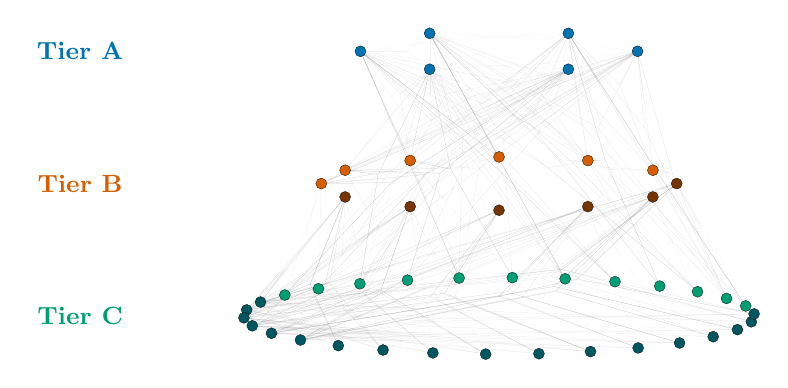
\begin{tikzpicture}[scale=1.4]
  \draw[gray, line width=0.08pt, opacity=0.10] (1.257,1.200) -- (0.419,1.309);
  \draw[gray, line width=0.08pt, opacity=0.10] (0.629,1.363) -- (0.419,1.309);
  \draw[gray, line width=0.08pt, opacity=0.10] (-0.629,1.363) -- (0.419,1.309);
  \draw[gray, line width=0.08pt, opacity=0.10] (1.257,1.200) -- (1.304,0.840);
  \draw[gray, line width=0.08pt, opacity=0.10] (1.396,0.121) -- (1.304,0.840);
  \draw[gray, line width=0.08pt, opacity=0.10] (1.257,1.200) -- (1.304,0.840);
  \draw[gray, line width=0.08pt, opacity=0.10] (1.257,1.200) -- (1.094,0.895);
  \draw[gray, line width=0.08pt, opacity=0.10] (1.396,0.121) -- (1.094,0.895);
  \draw[gray, line width=0.08pt, opacity=0.10] (0.629,1.363) -- (1.094,0.895);
  \draw[gray, line width=0.08pt, opacity=0.10] (1.257,1.200) -- (0.675,0.895);
  \draw[gray, line width=0.08pt, opacity=0.10] (1.396,0.121) -- (0.675,0.895);
  \draw[gray, line width=0.08pt, opacity=0.10] (-0.629,1.363) -- (0.675,0.895);
  \draw[gray, line width=0.08pt, opacity=0.10] (1.257,1.200) -- (0.301,0.800);
  \draw[gray, line width=0.08pt, opacity=0.10] (-1.612,0.000) -- (0.301,0.800);
  \draw[gray, line width=0.08pt, opacity=0.10] (1.257,1.200) -- (0.301,0.800);
  \draw[gray, line width=0.08pt, opacity=0.10] (1.257,1.200) -- (0.091,0.854);
  \draw[gray, line width=0.08pt, opacity=0.10] (-1.612,0.000) -- (0.091,0.854);
  \draw[gray, line width=0.08pt, opacity=0.10] (0.629,1.363) -- (0.091,0.854);
  \draw[gray, line width=0.08pt, opacity=0.10] (1.257,1.200) -- (-0.665,0.082);
  \draw[gray, line width=0.08pt, opacity=0.10] (-1.612,0.000) -- (-0.665,0.082);
  \draw[gray, line width=0.08pt, opacity=0.10] (-1.638,-0.954) -- (-0.665,0.082);
  \draw[gray, line width=0.08pt, opacity=0.10] (1.257,1.200) -- (1.317,0.507);
  \draw[gray, line width=0.08pt, opacity=0.10] (2.064,-1.042) -- (1.317,0.507);
  \draw[gray, line width=0.08pt, opacity=0.10] (0.629,1.363) -- (1.317,0.507);
  \draw[gray, line width=0.08pt, opacity=0.10] (1.257,1.200) -- (0.898,0.507);
  \draw[gray, line width=0.08pt, opacity=0.10] (2.064,-1.042) -- (0.898,0.507);
  \draw[gray, line width=0.08pt, opacity=0.10] (-0.629,1.363) -- (0.898,0.507);
  \draw[gray, line width=0.08pt, opacity=0.10] (1.257,1.200) -- (1.573,0.093);
  \draw[gray, line width=0.08pt, opacity=0.10] (2.064,-1.042) -- (1.573,0.093);
  \draw[gray, line width=0.08pt, opacity=0.10] (1.396,0.121) -- (1.573,0.093);
  \draw[gray, line width=0.08pt, opacity=0.10] (1.257,1.200) -- (0.292,0.482);
  \draw[gray, line width=0.08pt, opacity=0.10] (-1.638,-0.954) -- (0.292,0.482);
  \draw[gray, line width=0.08pt, opacity=0.10] (1.257,1.200) -- (0.292,0.482);
  \draw[gray, line width=0.08pt, opacity=0.10] (1.257,1.200) -- (-0.665,0.082);
  \draw[gray, line width=0.08pt, opacity=0.10] (-1.638,-0.954) -- (-0.665,0.082);
  \draw[gray, line width=0.08pt, opacity=0.10] (-1.612,0.000) -- (-0.665,0.082);
  \draw[gray, line width=0.08pt, opacity=0.10] (0.629,1.363) -- (-0.419,1.309);
  \draw[gray, line width=0.08pt, opacity=0.10] (-0.629,1.363) -- (-0.419,1.309);
  \draw[gray, line width=0.08pt, opacity=0.10] (-1.257,1.200) -- (-0.419,1.309);
  \draw[gray, line width=0.08pt, opacity=0.10] (0.629,1.363) -- (0.885,0.949);
  \draw[gray, line width=0.08pt, opacity=0.10] (1.396,0.121) -- (0.885,0.949);
  \draw[gray, line width=0.08pt, opacity=0.10] (0.629,1.363) -- (0.885,0.949);
  \draw[gray, line width=0.08pt, opacity=0.10] (0.629,1.363) -- (1.421,0.125);
  \draw[gray, line width=0.08pt, opacity=0.10] (1.396,0.121) -- (1.421,0.125);
  \draw[gray, line width=0.08pt, opacity=0.10] (2.238,-1.110) -- (1.421,0.125);
  \draw[gray, line width=0.08pt, opacity=0.10] (0.629,1.363) -- (0.688,0.979);
  \draw[gray, line width=0.08pt, opacity=0.10] (0.806,0.209) -- (0.688,0.979);
  \draw[gray, line width=0.08pt, opacity=0.10] (0.629,1.363) -- (0.688,0.979);
  \draw[gray, line width=0.08pt, opacity=0.10] (0.629,1.363) -- (0.269,0.979);
  \draw[gray, line width=0.08pt, opacity=0.10] (0.806,0.209) -- (0.269,0.979);
  \draw[gray, line width=0.08pt, opacity=0.10] (-0.629,1.363) -- (0.269,0.979);
  \draw[gray, line width=0.08pt, opacity=0.10] (0.629,1.363) -- (0.059,0.924);
  \draw[gray, line width=0.08pt, opacity=0.10] (0.806,0.209) -- (0.059,0.924);
  \draw[gray, line width=0.08pt, opacity=0.10] (-1.257,1.200) -- (0.059,0.924);
  \draw[gray, line width=0.08pt, opacity=0.10] (0.629,1.363) -- (1.165,0.539);
  \draw[gray, line width=0.08pt, opacity=0.10] (2.238,-1.110) -- (1.165,0.539);
  \draw[gray, line width=0.08pt, opacity=0.10] (0.629,1.363) -- (1.165,0.539);
  \draw[gray, line width=0.08pt, opacity=0.10] (0.629,1.363) -- (0.746,0.539);
  \draw[gray, line width=0.08pt, opacity=0.10] (2.238,-1.110) -- (0.746,0.539);
  \draw[gray, line width=0.08pt, opacity=0.10] (-0.629,1.363) -- (0.746,0.539);
  \draw[gray, line width=0.08pt, opacity=0.10] (0.629,1.363) -- (1.421,0.125);
  \draw[gray, line width=0.08pt, opacity=0.10] (2.238,-1.110) -- (1.421,0.125);
  \draw[gray, line width=0.08pt, opacity=0.10] (1.396,0.121) -- (1.421,0.125);
  \draw[gray, line width=0.08pt, opacity=0.10] (0.629,1.363) -- (0.486,0.599);
  \draw[gray, line width=0.08pt, opacity=0.10] (1.458,-0.930) -- (0.486,0.599);
  \draw[gray, line width=0.08pt, opacity=0.10] (-0.629,1.363) -- (0.486,0.599);
  \draw[gray, line width=0.08pt, opacity=0.10] (0.629,1.363) -- (0.276,0.544);
  \draw[gray, line width=0.08pt, opacity=0.10] (1.458,-0.930) -- (0.276,0.544);
  \draw[gray, line width=0.08pt, opacity=0.10] (-1.257,1.200) -- (0.276,0.544);
  \draw[gray, line width=0.08pt, opacity=0.10] (0.629,1.363) -- (0.964,0.214);
  \draw[gray, line width=0.08pt, opacity=0.10] (1.458,-0.930) -- (0.964,0.214);
  \draw[gray, line width=0.08pt, opacity=0.10] (0.806,0.209) -- (0.964,0.214);
  \draw[gray, line width=0.08pt, opacity=0.10] (-0.629,1.363) -- (-0.838,1.200);
  \draw[gray, line width=0.08pt, opacity=0.10] (-1.257,1.200) -- (-0.838,1.200);
  \draw[gray, line width=0.08pt, opacity=0.10] (-0.629,1.037) -- (-0.838,1.200);
  \draw[gray, line width=0.08pt, opacity=0.10] (-0.629,1.363) -- (-0.360,0.924);
  \draw[gray, line width=0.08pt, opacity=0.10] (0.806,0.209) -- (-0.360,0.924);
  \draw[gray, line width=0.08pt, opacity=0.10] (-1.257,1.200) -- (-0.360,0.924);
  \draw[gray, line width=0.08pt, opacity=0.10] (-0.629,1.363) -- (0.659,0.197);
  \draw[gray, line width=0.08pt, opacity=0.10] (0.806,0.209) -- (0.659,0.197);
  \draw[gray, line width=0.08pt, opacity=0.10] (1.801,-0.981) -- (0.659,0.197);
  \draw[gray, line width=0.08pt, opacity=0.10] (-0.629,1.363) -- (-0.419,0.990);
  \draw[gray, line width=0.08pt, opacity=0.10] (0.000,0.242) -- (-0.419,0.990);
  \draw[gray, line width=0.08pt, opacity=0.10] (-0.629,1.363) -- (-0.419,0.990);
  \draw[gray, line width=0.08pt, opacity=0.10] (-0.629,1.363) -- (-0.419,0.881);
  \draw[gray, line width=0.08pt, opacity=0.10] (0.000,0.242) -- (-0.419,0.881);
  \draw[gray, line width=0.08pt, opacity=0.10] (-0.629,1.037) -- (-0.419,0.881);
  \draw[gray, line width=0.08pt, opacity=0.10] (-0.629,1.363) -- (-0.010,0.247);
  \draw[gray, line width=0.08pt, opacity=0.10] (0.000,0.242) -- (-0.010,0.247);
  \draw[gray, line width=0.08pt, opacity=0.10] (0.600,-0.864) -- (-0.010,0.247);
  \draw[gray, line width=0.08pt, opacity=0.10] (-0.629,1.363) -- (0.181,0.582);
  \draw[gray, line width=0.08pt, opacity=0.10] (1.801,-0.981) -- (0.181,0.582);
  \draw[gray, line width=0.08pt, opacity=0.10] (-0.629,1.363) -- (0.181,0.582);
  \draw[gray, line width=0.08pt, opacity=0.10] (-0.629,1.363) -- (-0.028,0.527);
  \draw[gray, line width=0.08pt, opacity=0.10] (1.801,-0.981) -- (-0.028,0.527);
  \draw[gray, line width=0.08pt, opacity=0.10] (-1.257,1.200) -- (-0.028,0.527);
  \draw[gray, line width=0.08pt, opacity=0.10] (-0.629,1.363) -- (-0.219,0.621);
  \draw[gray, line width=0.08pt, opacity=0.10] (0.600,-0.864) -- (-0.219,0.621);
  \draw[gray, line width=0.08pt, opacity=0.10] (-0.629,1.363) -- (-0.219,0.621);
  \draw[gray, line width=0.08pt, opacity=0.10] (-0.629,1.363) -- (-0.429,0.566);
  \draw[gray, line width=0.08pt, opacity=0.10] (0.600,-0.864) -- (-0.429,0.566);
  \draw[gray, line width=0.08pt, opacity=0.10] (-1.257,1.200) -- (-0.429,0.566);
  \draw[gray, line width=0.08pt, opacity=0.10] (-0.629,1.363) -- (-0.219,0.512);
  \draw[gray, line width=0.08pt, opacity=0.10] (0.600,-0.864) -- (-0.219,0.512);
  \draw[gray, line width=0.08pt, opacity=0.10] (-0.629,1.037) -- (-0.219,0.512);
  \draw[gray, line width=0.08pt, opacity=0.10] (-1.257,1.200) -- (-0.419,1.091);
  \draw[gray, line width=0.08pt, opacity=0.10] (-0.629,1.037) -- (-0.419,1.091);
  \draw[gray, line width=0.08pt, opacity=0.10] (0.629,1.037) -- (-0.419,1.091);
  \draw[gray, line width=0.08pt, opacity=0.10] (-1.257,1.200) -- (-0.838,0.881);
  \draw[gray, line width=0.08pt, opacity=0.10] (0.000,0.242) -- (-0.838,0.881);
  \draw[gray, line width=0.08pt, opacity=0.10] (-1.257,1.200) -- (-0.838,0.881);
  \draw[gray, line width=0.08pt, opacity=0.10] (-1.257,1.200) -- (-0.629,0.826);
  \draw[gray, line width=0.08pt, opacity=0.10] (0.000,0.242) -- (-0.629,0.826);
  \draw[gray, line width=0.08pt, opacity=0.10] (-0.629,1.037) -- (-0.629,0.826);
  \draw[gray, line width=0.08pt, opacity=0.10] (-1.257,1.200) -- (-1.107,0.870);
  \draw[gray, line width=0.08pt, opacity=0.10] (-0.806,0.209) -- (-1.107,0.870);
  \draw[gray, line width=0.08pt, opacity=0.10] (-1.257,1.200) -- (-1.107,0.870);
  \draw[gray, line width=0.08pt, opacity=0.10] (-1.257,1.200) -- (-0.897,0.815);
  \draw[gray, line width=0.08pt, opacity=0.10] (-0.806,0.209) -- (-0.897,0.815);
  \draw[gray, line width=0.08pt, opacity=0.10] (-0.629,1.037) -- (-0.897,0.815);
  \draw[gray, line width=0.08pt, opacity=0.10] (-1.257,1.200) -- (-0.478,0.815);
  \draw[gray, line width=0.08pt, opacity=0.10] (-0.806,0.209) -- (-0.478,0.815);
  \draw[gray, line width=0.08pt, opacity=0.10] (0.629,1.037) -- (-0.478,0.815);
  \draw[gray, line width=0.08pt, opacity=0.10] (-1.257,1.200) -- (-0.809,0.184);
  \draw[gray, line width=0.08pt, opacity=0.10] (-0.806,0.209) -- (-0.809,0.184);
  \draw[gray, line width=0.08pt, opacity=0.10] (-0.362,-0.857) -- (-0.809,0.184);
  \draw[gray, line width=0.08pt, opacity=0.10] (-1.257,1.200) -- (-0.278,0.449);
  \draw[gray, line width=0.08pt, opacity=0.10] (1.052,-0.890) -- (-0.278,0.449);
  \draw[gray, line width=0.08pt, opacity=0.10] (-0.629,1.037) -- (-0.278,0.449);
  \draw[gray, line width=0.08pt, opacity=0.10] (-1.257,1.200) -- (-0.068,0.184);
  \draw[gray, line width=0.08pt, opacity=0.10] (1.052,-0.890) -- (-0.068,0.184);
  \draw[gray, line width=0.08pt, opacity=0.10] (0.000,0.242) -- (-0.068,0.184);
  \draw[gray, line width=0.08pt, opacity=0.10] (-1.257,1.200) -- (-0.959,0.514);
  \draw[gray, line width=0.08pt, opacity=0.10] (-0.362,-0.857) -- (-0.959,0.514);
  \draw[gray, line width=0.08pt, opacity=0.10] (-1.257,1.200) -- (-0.959,0.514);
  \draw[gray, line width=0.08pt, opacity=0.10] (-1.257,1.200) -- (-0.330,0.460);
  \draw[gray, line width=0.08pt, opacity=0.10] (-0.362,-0.857) -- (-0.330,0.460);
  \draw[gray, line width=0.08pt, opacity=0.10] (0.629,1.037) -- (-0.330,0.460);
  \draw[gray, line width=0.08pt, opacity=0.10] (-1.257,1.200) -- (-0.809,0.184);
  \draw[gray, line width=0.08pt, opacity=0.10] (-0.362,-0.857) -- (-0.809,0.184);
  \draw[gray, line width=0.08pt, opacity=0.10] (-0.806,0.209) -- (-0.809,0.184);
  \draw[gray, line width=0.08pt, opacity=0.10] (-0.629,1.037) -- (0.419,1.091);
  \draw[gray, line width=0.08pt, opacity=0.10] (0.629,1.037) -- (0.419,1.091);
  \draw[gray, line width=0.08pt, opacity=0.10] (1.257,1.200) -- (0.419,1.091);
  \draw[gray, line width=0.08pt, opacity=0.10] (-0.629,1.037) -- (-0.688,0.761);
  \draw[gray, line width=0.08pt, opacity=0.10] (-0.806,0.209) -- (-0.688,0.761);
  \draw[gray, line width=0.08pt, opacity=0.10] (-0.629,1.037) -- (-0.688,0.761);
  \draw[gray, line width=0.08pt, opacity=0.10] (-0.629,1.037) -- (-0.438,0.131);
  \draw[gray, line width=0.08pt, opacity=0.10] (-0.806,0.209) -- (-0.438,0.131);
  \draw[gray, line width=0.08pt, opacity=0.10] (0.121,-0.853) -- (-0.438,0.131);
  \draw[gray, line width=0.08pt, opacity=0.10] (-0.629,1.037) -- (-0.256,0.786);
  \draw[gray, line width=0.08pt, opacity=0.10] (-1.396,0.121) -- (-0.256,0.786);
  \draw[gray, line width=0.08pt, opacity=0.10] (1.257,1.200) -- (-0.256,0.786);
  \draw[gray, line width=0.08pt, opacity=0.10] (-0.629,1.037) -- (-0.885,0.731);
  \draw[gray, line width=0.08pt, opacity=0.10] (-1.396,0.121) -- (-0.885,0.731);
  \draw[gray, line width=0.08pt, opacity=0.10] (-0.629,1.037) -- (-0.885,0.731);
  \draw[gray, line width=0.08pt, opacity=0.10] (-0.629,1.037) -- (-1.096,0.083);
  \draw[gray, line width=0.08pt, opacity=0.10] (-1.396,0.121) -- (-1.096,0.083);
  \draw[gray, line width=0.08pt, opacity=0.10] (-1.262,-0.909) -- (-1.096,0.083);
  \draw[gray, line width=0.08pt, opacity=0.10] (-0.629,1.037) -- (-0.379,0.407);
  \draw[gray, line width=0.08pt, opacity=0.10] (0.121,-0.853) -- (-0.379,0.407);
  \draw[gray, line width=0.08pt, opacity=0.10] (-0.629,1.037) -- (-0.379,0.407);
  \draw[gray, line width=0.08pt, opacity=0.10] (-0.629,1.037) -- (0.040,0.407);
  \draw[gray, line width=0.08pt, opacity=0.10] (0.121,-0.853) -- (0.040,0.407);
  \draw[gray, line width=0.08pt, opacity=0.10] (0.629,1.037) -- (0.040,0.407);
  \draw[gray, line width=0.08pt, opacity=0.10] (-0.629,1.037) -- (-0.438,0.131);
  \draw[gray, line width=0.08pt, opacity=0.10] (0.121,-0.853) -- (-0.438,0.131);
  \draw[gray, line width=0.08pt, opacity=0.10] (-0.806,0.209) -- (-0.438,0.131);
  \draw[gray, line width=0.08pt, opacity=0.10] (-0.629,1.037) -- (-0.840,0.388);
  \draw[gray, line width=0.08pt, opacity=0.10] (-1.262,-0.909) -- (-0.840,0.388);
  \draw[gray, line width=0.08pt, opacity=0.10] (-0.629,1.037) -- (-0.840,0.388);
  \draw[gray, line width=0.08pt, opacity=0.10] (-0.629,1.037) -- (-0.421,0.388);
  \draw[gray, line width=0.08pt, opacity=0.10] (-1.262,-0.909) -- (-0.421,0.388);
  \draw[gray, line width=0.08pt, opacity=0.10] (0.629,1.037) -- (-0.421,0.388);
  \draw[gray, line width=0.08pt, opacity=0.10] (-0.629,1.037) -- (-1.096,0.083);
  \draw[gray, line width=0.08pt, opacity=0.10] (-1.262,-0.909) -- (-1.096,0.083);
  \draw[gray, line width=0.08pt, opacity=0.10] (-1.396,0.121) -- (-1.096,0.083);
  \draw[gray, line width=0.08pt, opacity=0.10] (0.629,1.037) -- (0.163,0.786);
  \draw[gray, line width=0.08pt, opacity=0.10] (-1.396,0.121) -- (0.163,0.786);
  \draw[gray, line width=0.08pt, opacity=0.10] (1.257,1.200) -- (0.163,0.786);
  \draw[gray, line width=0.08pt, opacity=0.10] (0.629,1.037) -- (-0.046,0.731);
  \draw[gray, line width=0.08pt, opacity=0.10] (-1.396,0.121) -- (-0.046,0.731);
  \draw[gray, line width=0.08pt, opacity=0.10] (0.629,1.037) -- (-0.046,0.731);
  \draw[gray, line width=0.08pt, opacity=0.10] (0.629,1.037) -- (-0.533,0.094);
  \draw[gray, line width=0.08pt, opacity=0.10] (-1.396,0.121) -- (-0.533,0.094);
  \draw[gray, line width=0.08pt, opacity=0.10] (-0.830,-0.876) -- (-0.533,0.094);
  \draw[gray, line width=0.08pt, opacity=0.10] (0.629,1.037) -- (0.091,0.746);
  \draw[gray, line width=0.08pt, opacity=0.10] (-1.612,0.000) -- (0.091,0.746);
  \draw[gray, line width=0.08pt, opacity=0.10] (1.257,1.200) -- (0.091,0.746);
  \draw[gray, line width=0.08pt, opacity=0.10] (0.629,1.037) -- (-0.118,0.691);
  \draw[gray, line width=0.08pt, opacity=0.10] (-1.612,0.000) -- (-0.118,0.691);
  \draw[gray, line width=0.08pt, opacity=0.10] (0.629,1.037) -- (-0.118,0.691);
  \draw[gray, line width=0.08pt, opacity=0.10] (0.629,1.037) -- (-0.976,0.009);
  \draw[gray, line width=0.08pt, opacity=0.10] (-1.612,0.000) -- (-0.976,0.009);
  \draw[gray, line width=0.08pt, opacity=0.10] (-1.943,-1.011) -- (-0.976,0.009);
  \draw[gray, line width=0.08pt, opacity=0.10] (0.629,1.037) -- (0.352,0.454);
  \draw[gray, line width=0.08pt, opacity=0.10] (-0.830,-0.876) -- (0.352,0.454);
  \draw[gray, line width=0.08pt, opacity=0.10] (1.257,1.200) -- (0.352,0.454);
  \draw[gray, line width=0.08pt, opacity=0.10] (0.629,1.037) -- (-0.533,0.094);
  \draw[gray, line width=0.08pt, opacity=0.10] (-0.830,-0.876) -- (-0.533,0.094);
  \draw[gray, line width=0.08pt, opacity=0.10] (-1.396,0.121) -- (-0.533,0.094);
  \draw[gray, line width=0.08pt, opacity=0.10] (0.629,1.037) -- (-0.019,0.409);
  \draw[gray, line width=0.08pt, opacity=0.10] (-1.943,-1.011) -- (-0.019,0.409);
  \draw[gray, line width=0.08pt, opacity=0.10] (1.257,1.200) -- (-0.019,0.409);
  \draw[gray, line width=0.08pt, opacity=0.10] (0.629,1.037) -- (-0.229,0.463);
  \draw[gray, line width=0.08pt, opacity=0.10] (-1.943,-1.011) -- (-0.229,0.463);
  \draw[gray, line width=0.08pt, opacity=0.10] (0.629,1.363) -- (-0.229,0.463);
  \draw[gray, line width=0.08pt, opacity=0.10] (0.629,1.037) -- (-0.976,0.009);
  \draw[gray, line width=0.08pt, opacity=0.10] (-1.943,-1.011) -- (-0.976,0.009);
  \draw[gray, line width=0.08pt, opacity=0.10] (-1.612,0.000) -- (-0.976,0.009);
  \draw[gray, line width=0.08pt, opacity=0.10] (1.396,0.121) -- (1.304,0.840);
  \draw[gray, line width=0.08pt, opacity=0.10] (1.257,1.200) -- (1.304,0.840);
  \draw[gray, line width=0.08pt, opacity=0.10] (1.257,1.200) -- (1.304,0.840);
  \draw[gray, line width=0.08pt, opacity=0.10] (1.396,0.121) -- (1.094,0.895);
  \draw[gray, line width=0.08pt, opacity=0.10] (1.257,1.200) -- (1.094,0.895);
  \draw[gray, line width=0.08pt, opacity=0.10] (0.629,1.363) -- (1.094,0.895);
  \draw[gray, line width=0.08pt, opacity=0.10] (1.396,0.121) -- (0.675,0.895);
  \draw[gray, line width=0.08pt, opacity=0.10] (1.257,1.200) -- (0.675,0.895);
  \draw[gray, line width=0.08pt, opacity=0.10] (-0.629,1.363) -- (0.675,0.895);
  \draw[gray, line width=0.08pt, opacity=0.10] (1.396,0.121) -- (1.573,0.093);
  \draw[gray, line width=0.08pt, opacity=0.10] (1.257,1.200) -- (1.573,0.093);
  \draw[gray, line width=0.08pt, opacity=0.10] (2.064,-1.042) -- (1.573,0.093);
  \draw[gray, line width=0.08pt, opacity=0.10] (1.396,0.121) -- (0.885,0.949);
  \draw[gray, line width=0.08pt, opacity=0.10] (0.629,1.363) -- (0.885,0.949);
  \draw[gray, line width=0.08pt, opacity=0.10] (0.629,1.363) -- (0.885,0.949);
  \draw[gray, line width=0.08pt, opacity=0.10] (1.396,0.121) -- (0.465,0.949);
  \draw[gray, line width=0.08pt, opacity=0.10] (0.629,1.363) -- (0.465,0.949);
  \draw[gray, line width=0.08pt, opacity=0.10] (-0.629,1.363) -- (0.465,0.949);
  \draw[gray, line width=0.08pt, opacity=0.10] (1.396,0.121) -- (1.421,0.125);
  \draw[gray, line width=0.08pt, opacity=0.10] (0.629,1.363) -- (1.421,0.125);
  \draw[gray, line width=0.08pt, opacity=0.10] (2.238,-1.110) -- (1.421,0.125);
  \draw[gray, line width=0.08pt, opacity=0.10] (1.396,0.121) -- (1.421,0.125);
  \draw[gray, line width=0.08pt, opacity=0.10] (2.238,-1.110) -- (1.421,0.125);
  \draw[gray, line width=0.08pt, opacity=0.10] (0.629,1.363) -- (1.421,0.125);
  \draw[gray, line width=0.08pt, opacity=0.10] (1.396,0.121) -- (1.002,0.125);
  \draw[gray, line width=0.08pt, opacity=0.10] (2.238,-1.110) -- (1.002,0.125);
  \draw[gray, line width=0.08pt, opacity=0.10] (-0.629,1.363) -- (1.002,0.125);
  \draw[gray, line width=0.08pt, opacity=0.10] (1.396,0.121) -- (1.677,-0.289);
  \draw[gray, line width=0.08pt, opacity=0.10] (2.238,-1.110) -- (1.677,-0.289);
  \draw[gray, line width=0.08pt, opacity=0.10] (1.396,0.121) -- (1.677,-0.289);
  \draw[gray, line width=0.08pt, opacity=0.10] (1.396,0.121) -- (1.363,0.147);
  \draw[gray, line width=0.08pt, opacity=0.10] (2.064,-1.042) -- (1.363,0.147);
  \draw[gray, line width=0.08pt, opacity=0.10] (0.629,1.363) -- (1.363,0.147);
  \draw[gray, line width=0.08pt, opacity=0.10] (1.396,0.121) -- (0.944,0.147);
  \draw[gray, line width=0.08pt, opacity=0.10] (2.064,-1.042) -- (0.944,0.147);
  \draw[gray, line width=0.08pt, opacity=0.10] (-0.629,1.363) -- (0.944,0.147);
  \draw[gray, line width=0.08pt, opacity=0.10] (1.396,0.121) -- (1.619,-0.267);
  \draw[gray, line width=0.08pt, opacity=0.10] (2.064,-1.042) -- (1.619,-0.267);
  \draw[gray, line width=0.08pt, opacity=0.10] (1.396,0.121) -- (1.619,-0.267);
  \draw[gray, line width=0.08pt, opacity=0.10] (0.806,0.209) -- (0.269,0.979);
  \draw[gray, line width=0.08pt, opacity=0.10] (0.629,1.363) -- (0.269,0.979);
  \draw[gray, line width=0.08pt, opacity=0.10] (-0.629,1.363) -- (0.269,0.979);
  \draw[gray, line width=0.08pt, opacity=0.10] (0.806,0.209) -- (0.059,0.924);
  \draw[gray, line width=0.08pt, opacity=0.10] (0.629,1.363) -- (0.059,0.924);
  \draw[gray, line width=0.08pt, opacity=0.10] (-1.257,1.200) -- (0.059,0.924);
  \draw[gray, line width=0.08pt, opacity=0.10] (0.806,0.209) -- (0.747,0.594);
  \draw[gray, line width=0.08pt, opacity=0.10] (0.629,1.363) -- (0.747,0.594);
  \draw[gray, line width=0.08pt, opacity=0.10] (0.806,0.209) -- (0.747,0.594);
  \draw[gray, line width=0.08pt, opacity=0.10] (0.806,0.209) -- (0.964,0.214);
  \draw[gray, line width=0.08pt, opacity=0.10] (0.629,1.363) -- (0.964,0.214);
  \draw[gray, line width=0.08pt, opacity=0.10] (1.458,-0.930) -- (0.964,0.214);
  \draw[gray, line width=0.08pt, opacity=0.10] (0.806,0.209) -- (-0.360,0.924);
  \draw[gray, line width=0.08pt, opacity=0.10] (-0.629,1.363) -- (-0.360,0.924);
  \draw[gray, line width=0.08pt, opacity=0.10] (-1.257,1.200) -- (-0.360,0.924);
  \draw[gray, line width=0.08pt, opacity=0.10] (0.806,0.209) -- (0.328,0.594);
  \draw[gray, line width=0.08pt, opacity=0.10] (-0.629,1.363) -- (0.328,0.594);
  \draw[gray, line width=0.08pt, opacity=0.10] (0.806,0.209) -- (0.328,0.594);
  \draw[gray, line width=0.08pt, opacity=0.10] (0.806,0.209) -- (0.659,0.197);
  \draw[gray, line width=0.08pt, opacity=0.10] (-0.629,1.363) -- (0.659,0.197);
  \draw[gray, line width=0.08pt, opacity=0.10] (1.801,-0.981) -- (0.659,0.197);
  \draw[gray, line width=0.08pt, opacity=0.10] (0.806,0.209) -- (0.450,0.143);
  \draw[gray, line width=0.08pt, opacity=0.10] (1.801,-0.981) -- (0.450,0.143);
  \draw[gray, line width=0.08pt, opacity=0.10] (-1.257,1.200) -- (0.450,0.143);
  \draw[gray, line width=0.08pt, opacity=0.10] (0.806,0.209) -- (1.138,-0.187);
  \draw[gray, line width=0.08pt, opacity=0.10] (1.801,-0.981) -- (1.138,-0.187);
  \draw[gray, line width=0.08pt, opacity=0.10] (0.806,0.209) -- (1.138,-0.187);
  \draw[gray, line width=0.08pt, opacity=0.10] (0.806,0.209) -- (0.964,0.214);
  \draw[gray, line width=0.08pt, opacity=0.10] (1.458,-0.930) -- (0.964,0.214);
  \draw[gray, line width=0.08pt, opacity=0.10] (0.629,1.363) -- (0.964,0.214);
  \draw[gray, line width=0.08pt, opacity=0.10] (0.806,0.209) -- (0.545,0.214);
  \draw[gray, line width=0.08pt, opacity=0.10] (1.458,-0.930) -- (0.545,0.214);
  \draw[gray, line width=0.08pt, opacity=0.10] (-0.629,1.363) -- (0.545,0.214);
  \draw[gray, line width=0.08pt, opacity=0.10] (0.806,0.209) -- (1.024,-0.170);
  \draw[gray, line width=0.08pt, opacity=0.10] (1.458,-0.930) -- (1.024,-0.170);
  \draw[gray, line width=0.08pt, opacity=0.10] (0.806,0.209) -- (1.024,-0.170);
  \draw[gray, line width=0.08pt, opacity=0.10] (0.000,0.242) -- (-0.419,0.990);
  \draw[gray, line width=0.08pt, opacity=0.10] (-0.629,1.363) -- (-0.419,0.990);
  \draw[gray, line width=0.08pt, opacity=0.10] (-0.629,1.363) -- (-0.419,0.990);
  \draw[gray, line width=0.08pt, opacity=0.10] (0.000,0.242) -- (-0.629,0.935);
  \draw[gray, line width=0.08pt, opacity=0.10] (-0.629,1.363) -- (-0.629,0.935);
  \draw[gray, line width=0.08pt, opacity=0.10] (-1.257,1.200) -- (-0.629,0.935);
  \draw[gray, line width=0.08pt, opacity=0.10] (0.000,0.242) -- (-0.210,0.616);
  \draw[gray, line width=0.08pt, opacity=0.10] (-0.629,1.363) -- (-0.210,0.616);
  \draw[gray, line width=0.08pt, opacity=0.10] (0.000,0.242) -- (-0.210,0.616);
  \draw[gray, line width=0.08pt, opacity=0.10] (0.000,0.242) -- (-0.010,0.247);
  \draw[gray, line width=0.08pt, opacity=0.10] (-0.629,1.363) -- (-0.010,0.247);
  \draw[gray, line width=0.08pt, opacity=0.10] (0.600,-0.864) -- (-0.010,0.247);
  \draw[gray, line width=0.08pt, opacity=0.10] (0.000,0.242) -- (-0.838,0.881);
  \draw[gray, line width=0.08pt, opacity=0.10] (-1.257,1.200) -- (-0.838,0.881);
  \draw[gray, line width=0.08pt, opacity=0.10] (-1.257,1.200) -- (-0.838,0.881);
  \draw[gray, line width=0.08pt, opacity=0.10] (0.000,0.242) -- (-0.419,0.561);
  \draw[gray, line width=0.08pt, opacity=0.10] (-1.257,1.200) -- (-0.419,0.561);
  \draw[gray, line width=0.08pt, opacity=0.10] (0.000,0.242) -- (-0.419,0.561);
  \draw[gray, line width=0.08pt, opacity=0.10] (0.000,0.242) -- (-0.068,0.184);
  \draw[gray, line width=0.08pt, opacity=0.10] (-1.257,1.200) -- (-0.068,0.184);
  \draw[gray, line width=0.08pt, opacity=0.10] (1.052,-0.890) -- (-0.068,0.184);
  \draw[gray, line width=0.08pt, opacity=0.10] (0.000,0.242) -- (-0.068,0.184);
  \draw[gray, line width=0.08pt, opacity=0.10] (1.052,-0.890) -- (-0.068,0.184);
  \draw[gray, line width=0.08pt, opacity=0.10] (-1.257,1.200) -- (-0.068,0.184);
  \draw[gray, line width=0.08pt, opacity=0.10] (0.000,0.242) -- (0.141,0.129);
  \draw[gray, line width=0.08pt, opacity=0.10] (1.052,-0.890) -- (0.141,0.129);
  \draw[gray, line width=0.08pt, opacity=0.10] (-0.629,1.037) -- (0.141,0.129);
  \draw[gray, line width=0.08pt, opacity=0.10] (0.000,0.242) -- (-0.010,0.247);
  \draw[gray, line width=0.08pt, opacity=0.10] (0.600,-0.864) -- (-0.010,0.247);
  \draw[gray, line width=0.08pt, opacity=0.10] (-0.629,1.363) -- (-0.010,0.247);
  \draw[gray, line width=0.08pt, opacity=0.10] (0.000,0.242) -- (-0.219,0.193);
  \draw[gray, line width=0.08pt, opacity=0.10] (0.600,-0.864) -- (-0.219,0.193);
  \draw[gray, line width=0.08pt, opacity=0.10] (-1.257,1.200) -- (-0.219,0.193);
  \draw[gray, line width=0.08pt, opacity=0.10] (0.000,0.242) -- (-0.010,0.138);
  \draw[gray, line width=0.08pt, opacity=0.10] (0.600,-0.864) -- (-0.010,0.138);
  \draw[gray, line width=0.08pt, opacity=0.10] (-0.629,1.037) -- (-0.010,0.138);
  \draw[gray, line width=0.08pt, opacity=0.10] (-0.806,0.209) -- (-1.107,0.870);
  \draw[gray, line width=0.08pt, opacity=0.10] (-1.257,1.200) -- (-1.107,0.870);
  \draw[gray, line width=0.08pt, opacity=0.10] (-1.257,1.200) -- (-1.107,0.870);
  \draw[gray, line width=0.08pt, opacity=0.10] (-0.806,0.209) -- (-0.897,0.815);
  \draw[gray, line width=0.08pt, opacity=0.10] (-1.257,1.200) -- (-0.897,0.815);
  \draw[gray, line width=0.08pt, opacity=0.10] (-0.629,1.037) -- (-0.897,0.815);
  \draw[gray, line width=0.08pt, opacity=0.10] (-0.806,0.209) -- (-0.478,0.815);
  \draw[gray, line width=0.08pt, opacity=0.10] (-1.257,1.200) -- (-0.478,0.815);
  \draw[gray, line width=0.08pt, opacity=0.10] (0.629,1.037) -- (-0.478,0.815);
  \draw[gray, line width=0.08pt, opacity=0.10] (-0.806,0.209) -- (-0.957,0.540);
  \draw[gray, line width=0.08pt, opacity=0.10] (-1.257,1.200) -- (-0.957,0.540);
  \draw[gray, line width=0.08pt, opacity=0.10] (-0.806,0.209) -- (-0.957,0.540);
  \draw[gray, line width=0.08pt, opacity=0.10] (-0.806,0.209) -- (-0.688,0.761);
  \draw[gray, line width=0.08pt, opacity=0.10] (-0.629,1.037) -- (-0.688,0.761);
  \draw[gray, line width=0.08pt, opacity=0.10] (-0.629,1.037) -- (-0.688,0.761);
  \draw[gray, line width=0.08pt, opacity=0.10] (-0.806,0.209) -- (-0.269,0.761);
  \draw[gray, line width=0.08pt, opacity=0.10] (-0.629,1.037) -- (-0.269,0.761);
  \draw[gray, line width=0.08pt, opacity=0.10] (0.629,1.037) -- (-0.269,0.761);
  \draw[gray, line width=0.08pt, opacity=0.10] (-0.806,0.209) -- (-0.747,0.485);
  \draw[gray, line width=0.08pt, opacity=0.10] (-0.629,1.037) -- (-0.747,0.485);
  \draw[gray, line width=0.08pt, opacity=0.10] (-0.806,0.209) -- (-0.747,0.485);
  \draw[gray, line width=0.08pt, opacity=0.10] (-0.806,0.209) -- (-0.438,0.131);
  \draw[gray, line width=0.08pt, opacity=0.10] (0.121,-0.853) -- (-0.438,0.131);
  \draw[gray, line width=0.08pt, opacity=0.10] (-0.629,1.037) -- (-0.438,0.131);
  \draw[gray, line width=0.08pt, opacity=0.10] (-0.806,0.209) -- (-0.019,0.131);
  \draw[gray, line width=0.08pt, opacity=0.10] (0.121,-0.853) -- (-0.019,0.131);
  \draw[gray, line width=0.08pt, opacity=0.10] (0.629,1.037) -- (-0.019,0.131);
  \draw[gray, line width=0.08pt, opacity=0.10] (-0.806,0.209) -- (-0.497,-0.145);
  \draw[gray, line width=0.08pt, opacity=0.10] (0.121,-0.853) -- (-0.497,-0.145);
  \draw[gray, line width=0.08pt, opacity=0.10] (-0.806,0.209) -- (-0.497,-0.145);
  \draw[gray, line width=0.08pt, opacity=0.10] (-0.806,0.209) -- (-0.809,0.184);
  \draw[gray, line width=0.08pt, opacity=0.10] (-0.362,-0.857) -- (-0.809,0.184);
  \draw[gray, line width=0.08pt, opacity=0.10] (-1.257,1.200) -- (-0.809,0.184);
  \draw[gray, line width=0.08pt, opacity=0.10] (-0.806,0.209) -- (-0.180,0.130);
  \draw[gray, line width=0.08pt, opacity=0.10] (-0.362,-0.857) -- (-0.180,0.130);
  \draw[gray, line width=0.08pt, opacity=0.10] (0.629,1.037) -- (-0.180,0.130);
  \draw[gray, line width=0.08pt, opacity=0.10] (-0.806,0.209) -- (-0.658,-0.146);
  \draw[gray, line width=0.08pt, opacity=0.10] (-0.362,-0.857) -- (-0.658,-0.146);
  \draw[gray, line width=0.08pt, opacity=0.10] (-0.806,0.209) -- (-0.658,-0.146);
  \draw[gray, line width=0.08pt, opacity=0.10] (-1.396,0.121) -- (-0.256,0.786);
  \draw[gray, line width=0.08pt, opacity=0.10] (-0.629,1.037) -- (-0.256,0.786);
  \draw[gray, line width=0.08pt, opacity=0.10] (1.257,1.200) -- (-0.256,0.786);
  \draw[gray, line width=0.08pt, opacity=0.10] (-1.396,0.121) -- (-0.465,0.731);
  \draw[gray, line width=0.08pt, opacity=0.10] (-0.629,1.037) -- (-0.465,0.731);
  \draw[gray, line width=0.08pt, opacity=0.10] (0.629,1.037) -- (-0.465,0.731);
  \draw[gray, line width=0.08pt, opacity=0.10] (-1.396,0.121) -- (-1.140,0.426);
  \draw[gray, line width=0.08pt, opacity=0.10] (-0.629,1.037) -- (-1.140,0.426);
  \draw[gray, line width=0.08pt, opacity=0.10] (-1.396,0.121) -- (-1.140,0.426);
  \draw[gray, line width=0.08pt, opacity=0.10] (-1.396,0.121) -- (-1.096,0.083);
  \draw[gray, line width=0.08pt, opacity=0.10] (-0.629,1.037) -- (-1.096,0.083);
  \draw[gray, line width=0.08pt, opacity=0.10] (-1.262,-0.909) -- (-1.096,0.083);
  \draw[gray, line width=0.08pt, opacity=0.10] (-1.396,0.121) -- (0.163,0.786);
  \draw[gray, line width=0.08pt, opacity=0.10] (0.629,1.037) -- (0.163,0.786);
  \draw[gray, line width=0.08pt, opacity=0.10] (1.257,1.200) -- (0.163,0.786);
  \draw[gray, line width=0.08pt, opacity=0.10] (-1.396,0.121) -- (-0.721,0.426);
  \draw[gray, line width=0.08pt, opacity=0.10] (0.629,1.037) -- (-0.721,0.426);
  \draw[gray, line width=0.08pt, opacity=0.10] (-1.396,0.121) -- (-0.721,0.426);
  \draw[gray, line width=0.08pt, opacity=0.10] (-1.396,0.121) -- (-0.533,0.094);
  \draw[gray, line width=0.08pt, opacity=0.10] (0.629,1.037) -- (-0.533,0.094);
  \draw[gray, line width=0.08pt, opacity=0.10] (-0.830,-0.876) -- (-0.533,0.094);
  \draw[gray, line width=0.08pt, opacity=0.10] (-1.396,0.121) -- (-0.323,0.148);
  \draw[gray, line width=0.08pt, opacity=0.10] (-0.830,-0.876) -- (-0.323,0.148);
  \draw[gray, line width=0.08pt, opacity=0.10] (1.257,1.200) -- (-0.323,0.148);
  \draw[gray, line width=0.08pt, opacity=0.10] (-1.396,0.121) -- (-1.208,-0.211);
  \draw[gray, line width=0.08pt, opacity=0.10] (-0.830,-0.876) -- (-1.208,-0.211);
  \draw[gray, line width=0.08pt, opacity=0.10] (-1.396,0.121) -- (-1.208,-0.211);
  \draw[gray, line width=0.08pt, opacity=0.10] (-1.396,0.121) -- (-0.467,0.137);
  \draw[gray, line width=0.08pt, opacity=0.10] (-1.262,-0.909) -- (-0.467,0.137);
  \draw[gray, line width=0.08pt, opacity=0.10] (1.257,1.200) -- (-0.467,0.137);
  \draw[gray, line width=0.08pt, opacity=0.10] (-1.396,0.121) -- (-1.096,0.083);
  \draw[gray, line width=0.08pt, opacity=0.10] (-1.262,-0.909) -- (-1.096,0.083);
  \draw[gray, line width=0.08pt, opacity=0.10] (-0.629,1.037) -- (-1.096,0.083);
  \draw[gray, line width=0.08pt, opacity=0.10] (-1.396,0.121) -- (-0.677,0.083);
  \draw[gray, line width=0.08pt, opacity=0.10] (-1.262,-0.909) -- (-0.677,0.083);
  \draw[gray, line width=0.08pt, opacity=0.10] (0.629,1.037) -- (-0.677,0.083);
  \draw[gray, line width=0.08pt, opacity=0.10] (-1.612,0.000) -- (0.301,0.800);
  \draw[gray, line width=0.08pt, opacity=0.10] (1.257,1.200) -- (0.301,0.800);
  \draw[gray, line width=0.08pt, opacity=0.10] (1.257,1.200) -- (0.301,0.800);
  \draw[gray, line width=0.08pt, opacity=0.10] (-1.612,0.000) -- (0.091,0.854);
  \draw[gray, line width=0.08pt, opacity=0.10] (1.257,1.200) -- (0.091,0.854);
  \draw[gray, line width=0.08pt, opacity=0.10] (0.629,1.363) -- (0.091,0.854);
  \draw[gray, line width=0.08pt, opacity=0.10] (-1.612,0.000) -- (-0.656,0.400);
  \draw[gray, line width=0.08pt, opacity=0.10] (1.257,1.200) -- (-0.656,0.400);
  \draw[gray, line width=0.08pt, opacity=0.10] (-1.612,0.000) -- (-0.656,0.400);
  \draw[gray, line width=0.08pt, opacity=0.10] (-1.612,0.000) -- (0.091,0.746);
  \draw[gray, line width=0.08pt, opacity=0.10] (0.629,1.037) -- (0.091,0.746);
  \draw[gray, line width=0.08pt, opacity=0.10] (1.257,1.200) -- (0.091,0.746);
  \draw[gray, line width=0.08pt, opacity=0.10] (-1.612,0.000) -- (-0.118,0.800);
  \draw[gray, line width=0.08pt, opacity=0.10] (0.629,1.037) -- (-0.118,0.800);
  \draw[gray, line width=0.08pt, opacity=0.10] (0.629,1.363) -- (-0.118,0.800);
  \draw[gray, line width=0.08pt, opacity=0.10] (-1.612,0.000) -- (-0.118,0.691);
  \draw[gray, line width=0.08pt, opacity=0.10] (0.629,1.037) -- (-0.118,0.691);
  \draw[gray, line width=0.08pt, opacity=0.10] (0.629,1.037) -- (-0.118,0.691);
  \draw[gray, line width=0.08pt, opacity=0.10] (-1.612,0.000) -- (-0.976,0.009);
  \draw[gray, line width=0.08pt, opacity=0.10] (0.629,1.037) -- (-0.976,0.009);
  \draw[gray, line width=0.08pt, opacity=0.10] (-1.943,-1.011) -- (-0.976,0.009);
  \draw[gray, line width=0.08pt, opacity=0.10] (-1.612,0.000) -- (-0.665,0.082);
  \draw[gray, line width=0.08pt, opacity=0.10] (-1.638,-0.954) -- (-0.665,0.082);
  \draw[gray, line width=0.08pt, opacity=0.10] (1.257,1.200) -- (-0.665,0.082);
  \draw[gray, line width=0.08pt, opacity=0.10] (-1.612,0.000) -- (-0.874,0.136);
  \draw[gray, line width=0.08pt, opacity=0.10] (-1.638,-0.954) -- (-0.874,0.136);
  \draw[gray, line width=0.08pt, opacity=0.10] (0.629,1.363) -- (-0.874,0.136);
  \draw[gray, line width=0.08pt, opacity=0.10] (-1.612,0.000) -- (-1.621,-0.318);
  \draw[gray, line width=0.08pt, opacity=0.10] (-1.638,-0.954) -- (-1.621,-0.318);
  \draw[gray, line width=0.08pt, opacity=0.10] (-1.612,0.000) -- (-1.621,-0.318);
  \draw[gray, line width=0.08pt, opacity=0.10] (-1.612,0.000) -- (-0.976,0.118);
  \draw[gray, line width=0.08pt, opacity=0.10] (-1.943,-1.011) -- (-0.976,0.118);
  \draw[gray, line width=0.08pt, opacity=0.10] (0.629,1.363) -- (-0.976,0.118);
  \draw[gray, line width=0.08pt, opacity=0.10] (-1.612,0.000) -- (-0.976,0.009);
  \draw[gray, line width=0.08pt, opacity=0.10] (-1.943,-1.011) -- (-0.976,0.009);
  \draw[gray, line width=0.08pt, opacity=0.10] (0.629,1.037) -- (-0.976,0.009);
  \draw[gray, line width=0.08pt, opacity=0.10] (-1.612,0.000) -- (-1.723,-0.337);
  \draw[gray, line width=0.08pt, opacity=0.10] (-1.943,-1.011) -- (-1.723,-0.337);
  \draw[gray, line width=0.08pt, opacity=0.10] (-1.612,0.000) -- (-1.723,-0.337);
  \draw[gray, line width=0.08pt, opacity=0.10] (2.238,-1.110) -- (0.746,0.539);
  \draw[gray, line width=0.08pt, opacity=0.10] (0.629,1.363) -- (0.746,0.539);
  \draw[gray, line width=0.08pt, opacity=0.10] (-0.629,1.363) -- (0.746,0.539);
  \draw[gray, line width=0.08pt, opacity=0.10] (2.238,-1.110) -- (1.421,0.125);
  \draw[gray, line width=0.08pt, opacity=0.10] (0.629,1.363) -- (1.421,0.125);
  \draw[gray, line width=0.08pt, opacity=0.10] (1.396,0.121) -- (1.421,0.125);
  \draw[gray, line width=0.08pt, opacity=0.10] (2.238,-1.110) -- (1.421,0.125);
  \draw[gray, line width=0.08pt, opacity=0.10] (1.396,0.121) -- (1.421,0.125);
  \draw[gray, line width=0.08pt, opacity=0.10] (0.629,1.363) -- (1.421,0.125);
  \draw[gray, line width=0.08pt, opacity=0.10] (2.238,-1.110) -- (1.002,0.125);
  \draw[gray, line width=0.08pt, opacity=0.10] (1.396,0.121) -- (1.002,0.125);
  \draw[gray, line width=0.08pt, opacity=0.10] (-0.629,1.363) -- (1.002,0.125);
  \draw[gray, line width=0.08pt, opacity=0.10] (2.064,-1.042) -- (1.317,0.507);
  \draw[gray, line width=0.08pt, opacity=0.10] (1.257,1.200) -- (1.317,0.507);
  \draw[gray, line width=0.08pt, opacity=0.10] (0.629,1.363) -- (1.317,0.507);
  \draw[gray, line width=0.08pt, opacity=0.10] (2.064,-1.042) -- (0.898,0.507);
  \draw[gray, line width=0.08pt, opacity=0.10] (1.257,1.200) -- (0.898,0.507);
  \draw[gray, line width=0.08pt, opacity=0.10] (-0.629,1.363) -- (0.898,0.507);
  \draw[gray, line width=0.08pt, opacity=0.10] (2.064,-1.042) -- (1.573,0.093);
  \draw[gray, line width=0.08pt, opacity=0.10] (1.257,1.200) -- (1.573,0.093);
  \draw[gray, line width=0.08pt, opacity=0.10] (1.396,0.121) -- (1.573,0.093);
  \draw[gray, line width=0.08pt, opacity=0.10] (2.064,-1.042) -- (1.363,0.147);
  \draw[gray, line width=0.08pt, opacity=0.10] (1.396,0.121) -- (1.363,0.147);
  \draw[gray, line width=0.08pt, opacity=0.10] (0.629,1.363) -- (1.363,0.147);
  \draw[gray, line width=0.08pt, opacity=0.10] (2.064,-1.042) -- (0.944,0.147);
  \draw[gray, line width=0.08pt, opacity=0.10] (1.396,0.121) -- (0.944,0.147);
  \draw[gray, line width=0.08pt, opacity=0.10] (-0.629,1.363) -- (0.944,0.147);
  \draw[gray, line width=0.08pt, opacity=0.10] (1.801,-0.981) -- (0.181,0.582);
  \draw[gray, line width=0.08pt, opacity=0.10] (-0.629,1.363) -- (0.181,0.582);
  \draw[gray, line width=0.08pt, opacity=0.10] (-0.629,1.363) -- (0.181,0.582);
  \draw[gray, line width=0.08pt, opacity=0.10] (1.801,-0.981) -- (-0.028,0.527);
  \draw[gray, line width=0.08pt, opacity=0.10] (-0.629,1.363) -- (-0.028,0.527);
  \draw[gray, line width=0.08pt, opacity=0.10] (-1.257,1.200) -- (-0.028,0.527);
  \draw[gray, line width=0.08pt, opacity=0.10] (1.801,-0.981) -- (0.659,0.197);
  \draw[gray, line width=0.08pt, opacity=0.10] (0.806,0.209) -- (0.659,0.197);
  \draw[gray, line width=0.08pt, opacity=0.10] (-0.629,1.363) -- (0.659,0.197);
  \draw[gray, line width=0.08pt, opacity=0.10] (1.801,-0.981) -- (0.450,0.143);
  \draw[gray, line width=0.08pt, opacity=0.10] (0.806,0.209) -- (0.450,0.143);
  \draw[gray, line width=0.08pt, opacity=0.10] (-1.257,1.200) -- (0.450,0.143);
  \draw[gray, line width=0.08pt, opacity=0.10] (1.458,-0.930) -- (0.905,0.599);
  \draw[gray, line width=0.08pt, opacity=0.10] (0.629,1.363) -- (0.905,0.599);
  \draw[gray, line width=0.08pt, opacity=0.10] (0.629,1.363) -- (0.905,0.599);
  \draw[gray, line width=0.08pt, opacity=0.10] (1.458,-0.930) -- (0.276,0.544);
  \draw[gray, line width=0.08pt, opacity=0.10] (0.629,1.363) -- (0.276,0.544);
  \draw[gray, line width=0.08pt, opacity=0.10] (-1.257,1.200) -- (0.276,0.544);
  \draw[gray, line width=0.08pt, opacity=0.10] (1.458,-0.930) -- (0.964,0.214);
  \draw[gray, line width=0.08pt, opacity=0.10] (0.629,1.363) -- (0.964,0.214);
  \draw[gray, line width=0.08pt, opacity=0.10] (0.806,0.209) -- (0.964,0.214);
  \draw[gray, line width=0.08pt, opacity=0.10] (1.458,-0.930) -- (0.964,0.214);
  \draw[gray, line width=0.08pt, opacity=0.10] (0.806,0.209) -- (0.964,0.214);
  \draw[gray, line width=0.08pt, opacity=0.10] (0.629,1.363) -- (0.964,0.214);
  \draw[gray, line width=0.08pt, opacity=0.10] (1.458,-0.930) -- (0.545,0.214);
  \draw[gray, line width=0.08pt, opacity=0.10] (0.806,0.209) -- (0.545,0.214);
  \draw[gray, line width=0.08pt, opacity=0.10] (-0.629,1.363) -- (0.545,0.214);
  \draw[gray, line width=0.08pt, opacity=0.10] (1.052,-0.890) -- (-0.488,0.503);
  \draw[gray, line width=0.08pt, opacity=0.10] (-1.257,1.200) -- (-0.488,0.503);
  \draw[gray, line width=0.08pt, opacity=0.10] (-1.257,1.200) -- (-0.488,0.503);
  \draw[gray, line width=0.08pt, opacity=0.10] (1.052,-0.890) -- (-0.278,0.449);
  \draw[gray, line width=0.08pt, opacity=0.10] (-1.257,1.200) -- (-0.278,0.449);
  \draw[gray, line width=0.08pt, opacity=0.10] (-0.629,1.037) -- (-0.278,0.449);
  \draw[gray, line width=0.08pt, opacity=0.10] (1.052,-0.890) -- (-0.068,0.184);
  \draw[gray, line width=0.08pt, opacity=0.10] (-1.257,1.200) -- (-0.068,0.184);
  \draw[gray, line width=0.08pt, opacity=0.10] (0.000,0.242) -- (-0.068,0.184);
  \draw[gray, line width=0.08pt, opacity=0.10] (1.052,-0.890) -- (0.141,0.129);
  \draw[gray, line width=0.08pt, opacity=0.10] (0.000,0.242) -- (0.141,0.129);
  \draw[gray, line width=0.08pt, opacity=0.10] (-0.629,1.037) -- (0.141,0.129);
  \draw[gray, line width=0.08pt, opacity=0.10] (0.600,-0.864) -- (-0.219,0.621);
  \draw[gray, line width=0.08pt, opacity=0.10] (-0.629,1.363) -- (-0.219,0.621);
  \draw[gray, line width=0.08pt, opacity=0.10] (-0.629,1.363) -- (-0.219,0.621);
  \draw[gray, line width=0.08pt, opacity=0.10] (0.600,-0.864) -- (-0.429,0.566);
  \draw[gray, line width=0.08pt, opacity=0.10] (-0.629,1.363) -- (-0.429,0.566);
  \draw[gray, line width=0.08pt, opacity=0.10] (-1.257,1.200) -- (-0.429,0.566);
  \draw[gray, line width=0.08pt, opacity=0.10] (0.600,-0.864) -- (-0.010,0.247);
  \draw[gray, line width=0.08pt, opacity=0.10] (-0.629,1.363) -- (-0.010,0.247);
  \draw[gray, line width=0.08pt, opacity=0.10] (0.000,0.242) -- (-0.010,0.247);
  \draw[gray, line width=0.08pt, opacity=0.10] (0.600,-0.864) -- (-0.010,0.247);
  \draw[gray, line width=0.08pt, opacity=0.10] (0.000,0.242) -- (-0.010,0.247);
  \draw[gray, line width=0.08pt, opacity=0.10] (-0.629,1.363) -- (-0.010,0.247);
  \draw[gray, line width=0.08pt, opacity=0.10] (0.600,-0.864) -- (-0.219,0.193);
  \draw[gray, line width=0.08pt, opacity=0.10] (0.000,0.242) -- (-0.219,0.193);
  \draw[gray, line width=0.08pt, opacity=0.10] (-1.257,1.200) -- (-0.219,0.193);
  \draw[gray, line width=0.08pt, opacity=0.10] (0.600,-0.864) -- (-0.010,0.138);
  \draw[gray, line width=0.08pt, opacity=0.10] (0.000,0.242) -- (-0.010,0.138);
  \draw[gray, line width=0.08pt, opacity=0.10] (-0.629,1.037) -- (-0.010,0.138);
  \draw[gray, line width=0.08pt, opacity=0.10] (0.121,-0.853) -- (0.040,0.407);
  \draw[gray, line width=0.08pt, opacity=0.10] (-0.629,1.037) -- (0.040,0.407);
  \draw[gray, line width=0.08pt, opacity=0.10] (0.629,1.037) -- (0.040,0.407);
  \draw[gray, line width=0.08pt, opacity=0.10] (0.121,-0.853) -- (-0.438,0.131);
  \draw[gray, line width=0.08pt, opacity=0.10] (-0.629,1.037) -- (-0.438,0.131);
  \draw[gray, line width=0.08pt, opacity=0.10] (-0.806,0.209) -- (-0.438,0.131);
  \draw[gray, line width=0.08pt, opacity=0.10] (0.121,-0.853) -- (-0.438,0.131);
  \draw[gray, line width=0.08pt, opacity=0.10] (-0.806,0.209) -- (-0.438,0.131);
  \draw[gray, line width=0.08pt, opacity=0.10] (-0.629,1.037) -- (-0.438,0.131);
  \draw[gray, line width=0.08pt, opacity=0.10] (-0.362,-0.857) -- (-0.959,0.514);
  \draw[gray, line width=0.08pt, opacity=0.10] (-1.257,1.200) -- (-0.959,0.514);
  \draw[gray, line width=0.08pt, opacity=0.10] (-1.257,1.200) -- (-0.959,0.514);
  \draw[gray, line width=0.08pt, opacity=0.10] (-0.362,-0.857) -- (-0.749,0.460);
  \draw[gray, line width=0.08pt, opacity=0.10] (-1.257,1.200) -- (-0.749,0.460);
  \draw[gray, line width=0.08pt, opacity=0.10] (-0.629,1.037) -- (-0.749,0.460);
  \draw[gray, line width=0.08pt, opacity=0.10] (-0.362,-0.857) -- (-0.330,0.460);
  \draw[gray, line width=0.08pt, opacity=0.10] (-1.257,1.200) -- (-0.330,0.460);
  \draw[gray, line width=0.08pt, opacity=0.10] (0.629,1.037) -- (-0.330,0.460);
  \draw[gray, line width=0.08pt, opacity=0.10] (-0.362,-0.857) -- (-0.809,0.184);
  \draw[gray, line width=0.08pt, opacity=0.10] (-1.257,1.200) -- (-0.809,0.184);
  \draw[gray, line width=0.08pt, opacity=0.10] (-0.806,0.209) -- (-0.809,0.184);
  \draw[gray, line width=0.08pt, opacity=0.10] (-0.362,-0.857) -- (-0.599,0.130);
  \draw[gray, line width=0.08pt, opacity=0.10] (-0.806,0.209) -- (-0.599,0.130);
  \draw[gray, line width=0.08pt, opacity=0.10] (-0.629,1.037) -- (-0.599,0.130);
  \draw[gray, line width=0.08pt, opacity=0.10] (-0.362,-0.857) -- (-0.180,0.130);
  \draw[gray, line width=0.08pt, opacity=0.10] (-0.806,0.209) -- (-0.180,0.130);
  \draw[gray, line width=0.08pt, opacity=0.10] (0.629,1.037) -- (-0.180,0.130);
  \draw[gray, line width=0.08pt, opacity=0.10] (-0.830,-0.876) -- (0.352,0.454);
  \draw[gray, line width=0.08pt, opacity=0.10] (0.629,1.037) -- (0.352,0.454);
  \draw[gray, line width=0.08pt, opacity=0.10] (1.257,1.200) -- (0.352,0.454);
  \draw[gray, line width=0.08pt, opacity=0.10] (-0.830,-0.876) -- (-0.533,0.094);
  \draw[gray, line width=0.08pt, opacity=0.10] (0.629,1.037) -- (-0.533,0.094);
  \draw[gray, line width=0.08pt, opacity=0.10] (-1.396,0.121) -- (-0.533,0.094);
  \draw[gray, line width=0.08pt, opacity=0.10] (-0.830,-0.876) -- (-0.323,0.148);
  \draw[gray, line width=0.08pt, opacity=0.10] (-1.396,0.121) -- (-0.323,0.148);
  \draw[gray, line width=0.08pt, opacity=0.10] (1.257,1.200) -- (-0.323,0.148);
  \draw[gray, line width=0.08pt, opacity=0.10] (-0.830,-0.876) -- (-0.533,0.094);
  \draw[gray, line width=0.08pt, opacity=0.10] (-1.396,0.121) -- (-0.533,0.094);
  \draw[gray, line width=0.08pt, opacity=0.10] (0.629,1.037) -- (-0.533,0.094);
  \draw[gray, line width=0.08pt, opacity=0.10] (-1.262,-0.909) -- (-0.211,0.443);
  \draw[gray, line width=0.08pt, opacity=0.10] (-0.629,1.037) -- (-0.211,0.443);
  \draw[gray, line width=0.08pt, opacity=0.10] (1.257,1.200) -- (-0.211,0.443);
  \draw[gray, line width=0.08pt, opacity=0.10] (-1.262,-0.909) -- (-0.421,0.388);
  \draw[gray, line width=0.08pt, opacity=0.10] (-0.629,1.037) -- (-0.421,0.388);
  \draw[gray, line width=0.08pt, opacity=0.10] (0.629,1.037) -- (-0.421,0.388);
  \draw[gray, line width=0.08pt, opacity=0.10] (-1.262,-0.909) -- (-1.096,0.083);
  \draw[gray, line width=0.08pt, opacity=0.10] (-0.629,1.037) -- (-1.096,0.083);
  \draw[gray, line width=0.08pt, opacity=0.10] (-1.396,0.121) -- (-1.096,0.083);
  \draw[gray, line width=0.08pt, opacity=0.10] (-1.262,-0.909) -- (-0.467,0.137);
  \draw[gray, line width=0.08pt, opacity=0.10] (-1.396,0.121) -- (-0.467,0.137);
  \draw[gray, line width=0.08pt, opacity=0.10] (1.257,1.200) -- (-0.467,0.137);
  \draw[gray, line width=0.08pt, opacity=0.10] (-1.262,-0.909) -- (-0.677,0.083);
  \draw[gray, line width=0.08pt, opacity=0.10] (-1.396,0.121) -- (-0.677,0.083);
  \draw[gray, line width=0.08pt, opacity=0.10] (0.629,1.037) -- (-0.677,0.083);
  \draw[gray, line width=0.08pt, opacity=0.10] (-1.638,-0.954) -- (0.292,0.482);
  \draw[gray, line width=0.08pt, opacity=0.10] (1.257,1.200) -- (0.292,0.482);
  \draw[gray, line width=0.08pt, opacity=0.10] (1.257,1.200) -- (0.292,0.482);
  \draw[gray, line width=0.08pt, opacity=0.10] (-1.638,-0.954) -- (0.083,0.536);
  \draw[gray, line width=0.08pt, opacity=0.10] (1.257,1.200) -- (0.083,0.536);
  \draw[gray, line width=0.08pt, opacity=0.10] (0.629,1.363) -- (0.083,0.536);
  \draw[gray, line width=0.08pt, opacity=0.10] (-1.638,-0.954) -- (-0.665,0.082);
  \draw[gray, line width=0.08pt, opacity=0.10] (1.257,1.200) -- (-0.665,0.082);
  \draw[gray, line width=0.08pt, opacity=0.10] (-1.612,0.000) -- (-0.665,0.082);
  \draw[gray, line width=0.08pt, opacity=0.10] (-1.638,-0.954) -- (-0.874,0.136);
  \draw[gray, line width=0.08pt, opacity=0.10] (-1.612,0.000) -- (-0.874,0.136);
  \draw[gray, line width=0.08pt, opacity=0.10] (0.629,1.363) -- (-0.874,0.136);
  \draw[gray, line width=0.08pt, opacity=0.10] (-1.943,-1.011) -- (-0.019,0.409);
  \draw[gray, line width=0.08pt, opacity=0.10] (0.629,1.037) -- (-0.019,0.409);
  \draw[gray, line width=0.08pt, opacity=0.10] (1.257,1.200) -- (-0.019,0.409);
  \draw[gray, line width=0.08pt, opacity=0.10] (-1.943,-1.011) -- (-0.229,0.463);
  \draw[gray, line width=0.08pt, opacity=0.10] (0.629,1.037) -- (-0.229,0.463);
  \draw[gray, line width=0.08pt, opacity=0.10] (0.629,1.363) -- (-0.229,0.463);
  \draw[gray, line width=0.08pt, opacity=0.10] (-1.943,-1.011) -- (-0.976,0.009);
  \draw[gray, line width=0.08pt, opacity=0.10] (0.629,1.037) -- (-0.976,0.009);
  \draw[gray, line width=0.08pt, opacity=0.10] (-1.612,0.000) -- (-0.976,0.009);
  \draw[gray, line width=0.08pt, opacity=0.10] (-1.943,-1.011) -- (-0.766,0.063);
  \draw[gray, line width=0.08pt, opacity=0.10] (-1.612,0.000) -- (-0.766,0.063);
  \draw[gray, line width=0.08pt, opacity=0.10] (1.257,1.200) -- (-0.766,0.063);
  \draw[gray, line width=0.08pt, opacity=0.10] (-1.943,-1.011) -- (-0.976,0.118);
  \draw[gray, line width=0.08pt, opacity=0.10] (-1.612,0.000) -- (-0.976,0.118);
  \draw[gray, line width=0.08pt, opacity=0.10] (0.629,1.363) -- (-0.976,0.118);
  \draw[gray, line width=0.08pt, opacity=0.10] (-2.163,-1.075) -- (-2.255,-1.146);
  \draw[gray, line width=0.08pt, opacity=0.10] (-2.289,-1.146) -- (-2.255,-1.146);
  \draw[gray, line width=0.08pt, opacity=0.10] (-2.314,-1.218) -- (-2.255,-1.146);
  \draw[gray, line width=0.08pt, opacity=0.10] (-2.163,-1.075) -- (-1.908,-0.757);
  \draw[gray, line width=0.08pt, opacity=0.10] (-1.396,-0.121) -- (-1.908,-0.757);
  \draw[gray, line width=0.08pt, opacity=0.10] (-2.163,-1.075) -- (-1.908,-0.757);
  \draw[gray, line width=0.08pt, opacity=0.10] (-2.163,-1.075) -- (-1.949,-0.781);
  \draw[gray, line width=0.08pt, opacity=0.10] (-1.396,-0.121) -- (-1.949,-0.781);
  \draw[gray, line width=0.08pt, opacity=0.10] (-2.289,-1.146) -- (-1.949,-0.781);
  \draw[gray, line width=0.08pt, opacity=0.10] (-2.163,-1.075) -- (-1.958,-0.805);
  \draw[gray, line width=0.08pt, opacity=0.10] (-1.396,-0.121) -- (-1.958,-0.805);
  \draw[gray, line width=0.08pt, opacity=0.10] (-2.314,-1.218) -- (-1.958,-0.805);
  \draw[gray, line width=0.08pt, opacity=0.10] (-2.163,-1.075) -- (-0.905,-0.717);
  \draw[gray, line width=0.08pt, opacity=0.10] (1.612,-0.000) -- (-0.905,-0.717);
  \draw[gray, line width=0.08pt, opacity=0.10] (-2.163,-1.075) -- (-0.905,-0.717);
  \draw[gray, line width=0.08pt, opacity=0.10] (-2.163,-1.075) -- (-0.946,-0.740);
  \draw[gray, line width=0.08pt, opacity=0.10] (1.612,-0.000) -- (-0.946,-0.740);
  \draw[gray, line width=0.08pt, opacity=0.10] (-2.289,-1.146) -- (-0.946,-0.740);
  \draw[gray, line width=0.08pt, opacity=0.10] (-2.163,-1.075) -- (0.579,-0.777);
  \draw[gray, line width=0.08pt, opacity=0.10] (1.612,-0.000) -- (0.579,-0.777);
  \draw[gray, line width=0.08pt, opacity=0.10] (2.289,-1.254) -- (0.579,-0.777);
  \draw[gray, line width=0.08pt, opacity=0.10] (-2.163,-1.075) -- (-1.835,-1.244);
  \draw[gray, line width=0.08pt, opacity=0.10] (-1.052,-1.510) -- (-1.835,-1.244);
  \draw[gray, line width=0.08pt, opacity=0.10] (-2.289,-1.146) -- (-1.835,-1.244);
  \draw[gray, line width=0.08pt, opacity=0.10] (-2.163,-1.075) -- (-1.843,-1.268);
  \draw[gray, line width=0.08pt, opacity=0.10] (-1.052,-1.510) -- (-1.843,-1.268);
  \draw[gray, line width=0.08pt, opacity=0.10] (-2.314,-1.218) -- (-1.843,-1.268);
  \draw[gray, line width=0.08pt, opacity=0.10] (-2.163,-1.075) -- (-1.537,-0.902);
  \draw[gray, line width=0.08pt, opacity=0.10] (-1.052,-1.510) -- (-1.537,-0.902);
  \draw[gray, line width=0.08pt, opacity=0.10] (-1.396,-0.121) -- (-1.537,-0.902);
  \draw[gray, line width=0.08pt, opacity=0.10] (-2.163,-1.075) -- (-0.679,-1.135);
  \draw[gray, line width=0.08pt, opacity=0.10] (2.289,-1.254) -- (-0.679,-1.135);
  \draw[gray, line width=0.08pt, opacity=0.10] (-2.163,-1.075) -- (-0.679,-1.135);
  \draw[gray, line width=0.08pt, opacity=0.10] (-2.163,-1.075) -- (0.579,-0.777);
  \draw[gray, line width=0.08pt, opacity=0.10] (2.289,-1.254) -- (0.579,-0.777);
  \draw[gray, line width=0.08pt, opacity=0.10] (1.612,-0.000) -- (0.579,-0.777);
  \draw[gray, line width=0.08pt, opacity=0.10] (-2.289,-1.146) -- (-2.280,-1.218);
  \draw[gray, line width=0.08pt, opacity=0.10] (-2.314,-1.218) -- (-2.280,-1.218);
  \draw[gray, line width=0.08pt, opacity=0.10] (-2.238,-1.290) -- (-2.280,-1.218);
  \draw[gray, line width=0.08pt, opacity=0.10] (-2.289,-1.146) -- (-1.991,-0.804);
  \draw[gray, line width=0.08pt, opacity=0.10] (-1.396,-0.121) -- (-1.991,-0.804);
  \draw[gray, line width=0.08pt, opacity=0.10] (-2.289,-1.146) -- (-1.991,-0.804);
  \draw[gray, line width=0.08pt, opacity=0.10] (-2.289,-1.146) -- (-1.714,-0.912);
  \draw[gray, line width=0.08pt, opacity=0.10] (-1.396,-0.121) -- (-1.714,-0.912);
  \draw[gray, line width=0.08pt, opacity=0.10] (-1.458,-1.470) -- (-1.714,-0.912);
  \draw[gray, line width=0.08pt, opacity=0.10] (-2.289,-1.146) -- (-1.794,-0.834);
  \draw[gray, line width=0.08pt, opacity=0.10] (-0.806,-0.209) -- (-1.794,-0.834);
  \draw[gray, line width=0.08pt, opacity=0.10] (-2.289,-1.146) -- (-1.794,-0.834);
  \draw[gray, line width=0.08pt, opacity=0.10] (-2.289,-1.146) -- (-1.803,-0.858);
  \draw[gray, line width=0.08pt, opacity=0.10] (-0.806,-0.209) -- (-1.803,-0.858);
  \draw[gray, line width=0.08pt, opacity=0.10] (-2.314,-1.218) -- (-1.803,-0.858);
  \draw[gray, line width=0.08pt, opacity=0.10] (-2.289,-1.146) -- (-1.778,-0.882);
  \draw[gray, line width=0.08pt, opacity=0.10] (-0.806,-0.209) -- (-1.778,-0.882);
  \draw[gray, line width=0.08pt, opacity=0.10] (-2.238,-1.290) -- (-1.778,-0.882);
  \draw[gray, line width=0.08pt, opacity=0.10] (-2.289,-1.146) -- (-2.012,-1.254);
  \draw[gray, line width=0.08pt, opacity=0.10] (-1.458,-1.470) -- (-2.012,-1.254);
  \draw[gray, line width=0.08pt, opacity=0.10] (-2.289,-1.146) -- (-2.012,-1.254);
  \draw[gray, line width=0.08pt, opacity=0.10] (-2.289,-1.146) -- (-2.020,-1.278);
  \draw[gray, line width=0.08pt, opacity=0.10] (-1.458,-1.470) -- (-2.020,-1.278);
  \draw[gray, line width=0.08pt, opacity=0.10] (-2.314,-1.218) -- (-2.020,-1.278);
  \draw[gray, line width=0.08pt, opacity=0.10] (-2.289,-1.146) -- (-1.714,-0.912);
  \draw[gray, line width=0.08pt, opacity=0.10] (-1.458,-1.470) -- (-1.714,-0.912);
  \draw[gray, line width=0.08pt, opacity=0.10] (-1.396,-0.121) -- (-1.714,-0.912);
  \draw[gray, line width=0.08pt, opacity=0.10] (-2.289,-1.146) -- (-1.575,-1.304);
  \draw[gray, line width=0.08pt, opacity=0.10] (-0.121,-1.547) -- (-1.575,-1.304);
  \draw[gray, line width=0.08pt, opacity=0.10] (-2.314,-1.218) -- (-1.575,-1.304);
  \draw[gray, line width=0.08pt, opacity=0.10] (-2.289,-1.146) -- (-1.549,-1.328);
  \draw[gray, line width=0.08pt, opacity=0.10] (-0.121,-1.547) -- (-1.549,-1.328);
  \draw[gray, line width=0.08pt, opacity=0.10] (-2.238,-1.290) -- (-1.549,-1.328);
  \draw[gray, line width=0.08pt, opacity=0.10] (-2.289,-1.146) -- (-1.072,-0.967);
  \draw[gray, line width=0.08pt, opacity=0.10] (-0.121,-1.547) -- (-1.072,-0.967);
  \draw[gray, line width=0.08pt, opacity=0.10] (-0.806,-0.209) -- (-1.072,-0.967);
  \draw[gray, line width=0.08pt, opacity=0.10] (-2.314,-1.218) -- (-2.205,-1.289);
  \draw[gray, line width=0.08pt, opacity=0.10] (-2.238,-1.290) -- (-2.205,-1.289);
  \draw[gray, line width=0.08pt, opacity=0.10] (-2.064,-1.358) -- (-2.205,-1.289);
  \draw[gray, line width=0.08pt, opacity=0.10] (-2.314,-1.218) -- (-1.786,-0.906);
  \draw[gray, line width=0.08pt, opacity=0.10] (-0.806,-0.209) -- (-1.786,-0.906);
  \draw[gray, line width=0.08pt, opacity=0.10] (-2.238,-1.290) -- (-1.786,-0.906);
  \draw[gray, line width=0.08pt, opacity=0.10] (-2.314,-1.218) -- (-1.240,-0.988);
  \draw[gray, line width=0.08pt, opacity=0.10] (-0.806,-0.209) -- (-1.240,-0.988);
  \draw[gray, line width=0.08pt, opacity=0.10] (-0.600,-1.536) -- (-1.240,-0.988);
  \draw[gray, line width=0.08pt, opacity=0.10] (-2.314,-1.218) -- (-1.543,-0.893);
  \draw[gray, line width=0.08pt, opacity=0.10] (-0.000,-0.242) -- (-1.543,-0.893);
  \draw[gray, line width=0.08pt, opacity=0.10] (-2.314,-1.218) -- (-1.543,-0.893);
  \draw[gray, line width=0.08pt, opacity=0.10] (-2.314,-1.218) -- (-1.459,-0.939);
  \draw[gray, line width=0.08pt, opacity=0.10] (-0.000,-0.242) -- (-1.459,-0.939);
  \draw[gray, line width=0.08pt, opacity=0.10] (-2.064,-1.358) -- (-1.459,-0.939);
  \draw[gray, line width=0.08pt, opacity=0.10] (-2.314,-1.218) -- (-0.495,-0.995);
  \draw[gray, line width=0.08pt, opacity=0.10] (-0.000,-0.242) -- (-0.495,-0.995);
  \draw[gray, line width=0.08pt, opacity=0.10] (0.830,-1.524) -- (-0.495,-0.995);
  \draw[gray, line width=0.08pt, opacity=0.10] (-2.314,-1.218) -- (-1.742,-1.324);
  \draw[gray, line width=0.08pt, opacity=0.10] (-0.600,-1.536) -- (-1.742,-1.324);
  \draw[gray, line width=0.08pt, opacity=0.10] (-2.314,-1.218) -- (-1.742,-1.324);
  \draw[gray, line width=0.08pt, opacity=0.10] (-2.314,-1.218) -- (-1.717,-1.348);
  \draw[gray, line width=0.08pt, opacity=0.10] (-0.600,-1.536) -- (-1.717,-1.348);
  \draw[gray, line width=0.08pt, opacity=0.10] (-2.238,-1.290) -- (-1.717,-1.348);
  \draw[gray, line width=0.08pt, opacity=0.10] (-2.314,-1.218) -- (-1.266,-1.320);
  \draw[gray, line width=0.08pt, opacity=0.10] (0.830,-1.524) -- (-1.266,-1.320);
  \draw[gray, line width=0.08pt, opacity=0.10] (-2.314,-1.218) -- (-1.266,-1.320);
  \draw[gray, line width=0.08pt, opacity=0.10] (-2.314,-1.218) -- (-1.241,-1.344);
  \draw[gray, line width=0.08pt, opacity=0.10] (0.830,-1.524) -- (-1.241,-1.344);
  \draw[gray, line width=0.08pt, opacity=0.10] (-2.238,-1.290) -- (-1.241,-1.344);
  \draw[gray, line width=0.08pt, opacity=0.10] (-2.314,-1.218) -- (-1.183,-1.367);
  \draw[gray, line width=0.08pt, opacity=0.10] (0.830,-1.524) -- (-1.183,-1.367);
  \draw[gray, line width=0.08pt, opacity=0.10] (-2.064,-1.358) -- (-1.183,-1.367);
  \draw[gray, line width=0.08pt, opacity=0.10] (-2.238,-1.290) -- (-2.034,-1.355);
  \draw[gray, line width=0.08pt, opacity=0.10] (-2.064,-1.358) -- (-2.034,-1.355);
  \draw[gray, line width=0.08pt, opacity=0.10] (-1.801,-1.419) -- (-2.034,-1.355);
  \draw[gray, line width=0.08pt, opacity=0.10] (-2.238,-1.290) -- (-1.492,-0.941);
  \draw[gray, line width=0.08pt, opacity=0.10] (-0.000,-0.242) -- (-1.492,-0.941);
  \draw[gray, line width=0.08pt, opacity=0.10] (-2.238,-1.290) -- (-1.492,-0.941);
  \draw[gray, line width=0.08pt, opacity=0.10] (-2.238,-1.290) -- (-1.434,-0.963);
  \draw[gray, line width=0.08pt, opacity=0.10] (-0.000,-0.242) -- (-1.434,-0.963);
  \draw[gray, line width=0.08pt, opacity=0.10] (-2.064,-1.358) -- (-1.434,-0.963);
  \draw[gray, line width=0.08pt, opacity=0.10] (-2.238,-1.290) -- (-1.223,-0.930);
  \draw[gray, line width=0.08pt, opacity=0.10] (0.806,-0.209) -- (-1.223,-0.930);
  \draw[gray, line width=0.08pt, opacity=0.10] (-2.238,-1.290) -- (-1.223,-0.930);
  \draw[gray, line width=0.08pt, opacity=0.10] (-2.238,-1.290) -- (-1.165,-0.952);
  \draw[gray, line width=0.08pt, opacity=0.10] (0.806,-0.209) -- (-1.165,-0.952);
  \draw[gray, line width=0.08pt, opacity=0.10] (-2.064,-1.358) -- (-1.165,-0.952);
  \draw[gray, line width=0.08pt, opacity=0.10] (-2.238,-1.290) -- (-1.078,-0.973);
  \draw[gray, line width=0.08pt, opacity=0.10] (0.806,-0.209) -- (-1.078,-0.973);
  \draw[gray, line width=0.08pt, opacity=0.10] (-1.801,-1.419) -- (-1.078,-0.973);
  \draw[gray, line width=0.08pt, opacity=0.10] (-2.238,-1.290) -- (0.069,-0.982);
  \draw[gray, line width=0.08pt, opacity=0.10] (0.806,-0.209) -- (0.069,-0.982);
  \draw[gray, line width=0.08pt, opacity=0.10] (1.638,-1.446) -- (0.069,-0.982);
  \draw[gray, line width=0.08pt, opacity=0.10] (-2.238,-1.290) -- (-1.313,-1.397);
  \draw[gray, line width=0.08pt, opacity=0.10] (0.362,-1.543) -- (-1.313,-1.397);
  \draw[gray, line width=0.08pt, opacity=0.10] (-2.064,-1.358) -- (-1.313,-1.397);
  \draw[gray, line width=0.08pt, opacity=0.10] (-2.238,-1.290) -- (-0.625,-1.025);
  \draw[gray, line width=0.08pt, opacity=0.10] (0.362,-1.543) -- (-0.625,-1.025);
  \draw[gray, line width=0.08pt, opacity=0.10] (-0.000,-0.242) -- (-0.625,-1.025);
  \draw[gray, line width=0.08pt, opacity=0.10] (-2.238,-1.290) -- (-0.946,-1.342);
  \draw[gray, line width=0.08pt, opacity=0.10] (1.638,-1.446) -- (-0.946,-1.342);
  \draw[gray, line width=0.08pt, opacity=0.10] (-2.238,-1.290) -- (-0.946,-1.342);
  \draw[gray, line width=0.08pt, opacity=0.10] (-2.238,-1.290) -- (-0.800,-1.385);
  \draw[gray, line width=0.08pt, opacity=0.10] (1.638,-1.446) -- (-0.800,-1.385);
  \draw[gray, line width=0.08pt, opacity=0.10] (-1.801,-1.419) -- (-0.800,-1.385);
  \draw[gray, line width=0.08pt, opacity=0.10] (-2.238,-1.290) -- (0.069,-0.982);
  \draw[gray, line width=0.08pt, opacity=0.10] (1.638,-1.446) -- (0.069,-0.982);
  \draw[gray, line width=0.08pt, opacity=0.10] (0.806,-0.209) -- (0.069,-0.982);
  \draw[gray, line width=0.08pt, opacity=0.10] (-2.064,-1.358) -- (-2.009,-1.284);
  \draw[gray, line width=0.08pt, opacity=0.10] (-1.801,-1.419) -- (-2.009,-1.284);
  \draw[gray, line width=0.08pt, opacity=0.10] (-2.163,-1.075) -- (-2.009,-1.284);
  \draw[gray, line width=0.08pt, opacity=0.10] (-2.064,-1.358) -- (-1.108,-0.975);
  \draw[gray, line width=0.08pt, opacity=0.10] (0.806,-0.209) -- (-1.108,-0.975);
  \draw[gray, line width=0.08pt, opacity=0.10] (-2.064,-1.358) -- (-1.108,-0.975);
  \draw[gray, line width=0.08pt, opacity=0.10] (-2.064,-1.358) -- (0.001,-1.020);
  \draw[gray, line width=0.08pt, opacity=0.10] (0.806,-0.209) -- (0.001,-1.020);
  \draw[gray, line width=0.08pt, opacity=0.10] (1.262,-1.491) -- (0.001,-1.020);
  \draw[gray, line width=0.08pt, opacity=0.10] (-2.064,-1.358) -- (-0.944,-0.851);
  \draw[gray, line width=0.08pt, opacity=0.10] (1.396,-0.121) -- (-0.944,-0.851);
  \draw[gray, line width=0.08pt, opacity=0.10] (-2.163,-1.075) -- (-0.944,-0.851);
  \draw[gray, line width=0.08pt, opacity=0.10] (-2.064,-1.358) -- (-0.911,-0.946);
  \draw[gray, line width=0.08pt, opacity=0.10] (1.396,-0.121) -- (-0.911,-0.946);
  \draw[gray, line width=0.08pt, opacity=0.10] (-2.064,-1.358) -- (-0.911,-0.946);
  \draw[gray, line width=0.08pt, opacity=0.10] (-2.064,-1.358) -- (0.498,-0.934);
  \draw[gray, line width=0.08pt, opacity=0.10] (1.396,-0.121) -- (0.498,-0.934);
  \draw[gray, line width=0.08pt, opacity=0.10] (2.163,-1.325) -- (0.498,-0.934);
  \draw[gray, line width=0.08pt, opacity=0.10] (-2.064,-1.358) -- (-0.956,-1.402);
  \draw[gray, line width=0.08pt, opacity=0.10] (1.262,-1.491) -- (-0.956,-1.402);
  \draw[gray, line width=0.08pt, opacity=0.10] (-2.064,-1.358) -- (-0.956,-1.402);
  \draw[gray, line width=0.08pt, opacity=0.10] (-2.064,-1.358) -- (-0.868,-1.423);
  \draw[gray, line width=0.08pt, opacity=0.10] (1.262,-1.491) -- (-0.868,-1.423);
  \draw[gray, line width=0.08pt, opacity=0.10] (-1.801,-1.419) -- (-0.868,-1.423);
  \draw[gray, line width=0.08pt, opacity=0.10] (-2.064,-1.358) -- (0.001,-1.020);
  \draw[gray, line width=0.08pt, opacity=0.10] (1.262,-1.491) -- (0.001,-1.020);
  \draw[gray, line width=0.08pt, opacity=0.10] (0.806,-0.209) -- (0.001,-1.020);
  \draw[gray, line width=0.08pt, opacity=0.10] (-2.064,-1.358) -- (-0.655,-1.347);
  \draw[gray, line width=0.08pt, opacity=0.10] (2.163,-1.325) -- (-0.655,-1.347);
  \draw[gray, line width=0.08pt, opacity=0.10] (-2.064,-1.358) -- (-0.655,-1.347);
  \draw[gray, line width=0.08pt, opacity=0.10] (-2.064,-1.358) -- (-0.567,-1.367);
  \draw[gray, line width=0.08pt, opacity=0.10] (2.163,-1.325) -- (-0.567,-1.367);
  \draw[gray, line width=0.08pt, opacity=0.10] (-1.801,-1.419) -- (-0.567,-1.367);
  \draw[gray, line width=0.08pt, opacity=0.10] (-2.064,-1.358) -- (0.498,-0.934);
  \draw[gray, line width=0.08pt, opacity=0.10] (2.163,-1.325) -- (0.498,-0.934);
  \draw[gray, line width=0.08pt, opacity=0.10] (1.396,-0.121) -- (0.498,-0.934);
  \draw[gray, line width=0.08pt, opacity=0.10] (-1.801,-1.419) -- (-0.856,-0.872);
  \draw[gray, line width=0.08pt, opacity=0.10] (1.396,-0.121) -- (-0.856,-0.872);
  \draw[gray, line width=0.08pt, opacity=0.10] (-2.163,-1.075) -- (-0.856,-0.872);
  \draw[gray, line width=0.08pt, opacity=0.10] (-1.801,-1.419) -- (-0.735,-0.986);
  \draw[gray, line width=0.08pt, opacity=0.10] (1.396,-0.121) -- (-0.735,-0.986);
  \draw[gray, line width=0.08pt, opacity=0.10] (-1.801,-1.419) -- (-0.735,-0.986);
  \draw[gray, line width=0.08pt, opacity=0.10] (-1.801,-1.419) -- (0.513,-0.976);
  \draw[gray, line width=0.08pt, opacity=0.10] (1.396,-0.121) -- (0.513,-0.976);
  \draw[gray, line width=0.08pt, opacity=0.10] (1.943,-1.389) -- (0.513,-0.976);
  \draw[gray, line width=0.08pt, opacity=0.10] (-1.801,-1.419) -- (-0.784,-0.831);
  \draw[gray, line width=0.08pt, opacity=0.10] (1.612,-0.000) -- (-0.784,-0.831);
  \draw[gray, line width=0.08pt, opacity=0.10] (-2.163,-1.075) -- (-0.784,-0.831);
  \draw[gray, line width=0.08pt, opacity=0.10] (-1.801,-1.419) -- (-0.663,-0.946);
  \draw[gray, line width=0.08pt, opacity=0.10] (1.612,-0.000) -- (-0.663,-0.946);
  \draw[gray, line width=0.08pt, opacity=0.10] (-1.801,-1.419) -- (-0.663,-0.946);
  \draw[gray, line width=0.08pt, opacity=0.10] (-1.801,-1.419) -- (0.709,-0.867);
  \draw[gray, line width=0.08pt, opacity=0.10] (1.612,-0.000) -- (0.709,-0.867);
  \draw[gray, line width=0.08pt, opacity=0.10] (2.314,-1.182) -- (0.709,-0.867);
  \draw[gray, line width=0.08pt, opacity=0.10] (-1.801,-1.419) -- (-0.674,-1.294);
  \draw[gray, line width=0.08pt, opacity=0.10] (1.943,-1.389) -- (-0.674,-1.294);
  \draw[gray, line width=0.08pt, opacity=0.10] (-2.163,-1.075) -- (-0.674,-1.294);
  \draw[gray, line width=0.08pt, opacity=0.10] (-1.801,-1.419) -- (0.513,-0.976);
  \draw[gray, line width=0.08pt, opacity=0.10] (1.943,-1.389) -- (0.513,-0.976);
  \draw[gray, line width=0.08pt, opacity=0.10] (1.396,-0.121) -- (0.513,-0.976);
  \draw[gray, line width=0.08pt, opacity=0.10] (-1.801,-1.419) -- (-0.550,-1.225);
  \draw[gray, line width=0.08pt, opacity=0.10] (2.314,-1.182) -- (-0.550,-1.225);
  \draw[gray, line width=0.08pt, opacity=0.10] (-2.163,-1.075) -- (-0.550,-1.225);
  \draw[gray, line width=0.08pt, opacity=0.10] (-1.801,-1.419) -- (-0.592,-1.249);
  \draw[gray, line width=0.08pt, opacity=0.10] (2.314,-1.182) -- (-0.592,-1.249);
  \draw[gray, line width=0.08pt, opacity=0.10] (-2.289,-1.146) -- (-0.592,-1.249);
  \draw[gray, line width=0.08pt, opacity=0.10] (-1.801,-1.419) -- (0.709,-0.867);
  \draw[gray, line width=0.08pt, opacity=0.10] (2.314,-1.182) -- (0.709,-0.867);
  \draw[gray, line width=0.08pt, opacity=0.10] (1.612,-0.000) -- (0.709,-0.867);
  \draw[gray, line width=0.08pt, opacity=0.10] (-1.396,-0.121) -- (-1.908,-0.757);
  \draw[gray, line width=0.08pt, opacity=0.10] (-2.163,-1.075) -- (-1.908,-0.757);
  \draw[gray, line width=0.08pt, opacity=0.10] (-2.163,-1.075) -- (-1.908,-0.757);
  \draw[gray, line width=0.08pt, opacity=0.10] (-1.396,-0.121) -- (-1.949,-0.781);
  \draw[gray, line width=0.08pt, opacity=0.10] (-2.163,-1.075) -- (-1.949,-0.781);
  \draw[gray, line width=0.08pt, opacity=0.10] (-2.289,-1.146) -- (-1.949,-0.781);
  \draw[gray, line width=0.08pt, opacity=0.10] (-1.396,-0.121) -- (-1.958,-0.805);
  \draw[gray, line width=0.08pt, opacity=0.10] (-2.163,-1.075) -- (-1.958,-0.805);
  \draw[gray, line width=0.08pt, opacity=0.10] (-2.314,-1.218) -- (-1.958,-0.805);
  \draw[gray, line width=0.08pt, opacity=0.10] (-1.396,-0.121) -- (-1.537,-0.902);
  \draw[gray, line width=0.08pt, opacity=0.10] (-2.163,-1.075) -- (-1.537,-0.902);
  \draw[gray, line width=0.08pt, opacity=0.10] (-1.052,-1.510) -- (-1.537,-0.902);
  \draw[gray, line width=0.08pt, opacity=0.10] (-1.396,-0.121) -- (-1.991,-0.804);
  \draw[gray, line width=0.08pt, opacity=0.10] (-2.289,-1.146) -- (-1.991,-0.804);
  \draw[gray, line width=0.08pt, opacity=0.10] (-2.289,-1.146) -- (-1.991,-0.804);
  \draw[gray, line width=0.08pt, opacity=0.10] (-1.396,-0.121) -- (-2.000,-0.828);
  \draw[gray, line width=0.08pt, opacity=0.10] (-2.289,-1.146) -- (-2.000,-0.828);
  \draw[gray, line width=0.08pt, opacity=0.10] (-2.314,-1.218) -- (-2.000,-0.828);
  \draw[gray, line width=0.08pt, opacity=0.10] (-1.396,-0.121) -- (-1.714,-0.912);
  \draw[gray, line width=0.08pt, opacity=0.10] (-2.289,-1.146) -- (-1.714,-0.912);
  \draw[gray, line width=0.08pt, opacity=0.10] (-1.458,-1.470) -- (-1.714,-0.912);
  \draw[gray, line width=0.08pt, opacity=0.10] (-1.396,-0.121) -- (-1.714,-0.912);
  \draw[gray, line width=0.08pt, opacity=0.10] (-1.458,-1.470) -- (-1.714,-0.912);
  \draw[gray, line width=0.08pt, opacity=0.10] (-2.289,-1.146) -- (-1.714,-0.912);
  \draw[gray, line width=0.08pt, opacity=0.10] (-1.396,-0.121) -- (-1.723,-0.936);
  \draw[gray, line width=0.08pt, opacity=0.10] (-1.458,-1.470) -- (-1.723,-0.936);
  \draw[gray, line width=0.08pt, opacity=0.10] (-2.314,-1.218) -- (-1.723,-0.936);
  \draw[gray, line width=0.08pt, opacity=0.10] (-1.396,-0.121) -- (-1.417,-0.571);
  \draw[gray, line width=0.08pt, opacity=0.10] (-1.458,-1.470) -- (-1.417,-0.571);
  \draw[gray, line width=0.08pt, opacity=0.10] (-1.396,-0.121) -- (-1.417,-0.571);
  \draw[gray, line width=0.08pt, opacity=0.10] (-1.396,-0.121) -- (-1.579,-0.925);
  \draw[gray, line width=0.08pt, opacity=0.10] (-1.052,-1.510) -- (-1.579,-0.925);
  \draw[gray, line width=0.08pt, opacity=0.10] (-2.289,-1.146) -- (-1.579,-0.925);
  \draw[gray, line width=0.08pt, opacity=0.10] (-1.396,-0.121) -- (-1.587,-0.950);
  \draw[gray, line width=0.08pt, opacity=0.10] (-1.052,-1.510) -- (-1.587,-0.950);
  \draw[gray, line width=0.08pt, opacity=0.10] (-2.314,-1.218) -- (-1.587,-0.950);
  \draw[gray, line width=0.08pt, opacity=0.10] (-1.396,-0.121) -- (-1.282,-0.584);
  \draw[gray, line width=0.08pt, opacity=0.10] (-1.052,-1.510) -- (-1.282,-0.584);
  \draw[gray, line width=0.08pt, opacity=0.10] (-1.396,-0.121) -- (-1.282,-0.584);
  \draw[gray, line width=0.08pt, opacity=0.10] (-0.806,-0.209) -- (-1.803,-0.858);
  \draw[gray, line width=0.08pt, opacity=0.10] (-2.289,-1.146) -- (-1.803,-0.858);
  \draw[gray, line width=0.08pt, opacity=0.10] (-2.314,-1.218) -- (-1.803,-0.858);
  \draw[gray, line width=0.08pt, opacity=0.10] (-0.806,-0.209) -- (-1.778,-0.882);
  \draw[gray, line width=0.08pt, opacity=0.10] (-2.289,-1.146) -- (-1.778,-0.882);
  \draw[gray, line width=0.08pt, opacity=0.10] (-2.238,-1.290) -- (-1.778,-0.882);
  \draw[gray, line width=0.08pt, opacity=0.10] (-0.806,-0.209) -- (-1.300,-0.522);
  \draw[gray, line width=0.08pt, opacity=0.10] (-2.289,-1.146) -- (-1.300,-0.522);
  \draw[gray, line width=0.08pt, opacity=0.10] (-0.806,-0.209) -- (-1.300,-0.522);
  \draw[gray, line width=0.08pt, opacity=0.10] (-0.806,-0.209) -- (-1.072,-0.967);
  \draw[gray, line width=0.08pt, opacity=0.10] (-2.289,-1.146) -- (-1.072,-0.967);
  \draw[gray, line width=0.08pt, opacity=0.10] (-0.121,-1.547) -- (-1.072,-0.967);
  \draw[gray, line width=0.08pt, opacity=0.10] (-0.806,-0.209) -- (-1.786,-0.906);
  \draw[gray, line width=0.08pt, opacity=0.10] (-2.314,-1.218) -- (-1.786,-0.906);
  \draw[gray, line width=0.08pt, opacity=0.10] (-2.238,-1.290) -- (-1.786,-0.906);
  \draw[gray, line width=0.08pt, opacity=0.10] (-0.806,-0.209) -- (-1.309,-0.546);
  \draw[gray, line width=0.08pt, opacity=0.10] (-2.314,-1.218) -- (-1.309,-0.546);
  \draw[gray, line width=0.08pt, opacity=0.10] (-0.806,-0.209) -- (-1.309,-0.546);
  \draw[gray, line width=0.08pt, opacity=0.10] (-0.806,-0.209) -- (-1.240,-0.988);
  \draw[gray, line width=0.08pt, opacity=0.10] (-2.314,-1.218) -- (-1.240,-0.988);
  \draw[gray, line width=0.08pt, opacity=0.10] (-0.600,-1.536) -- (-1.240,-0.988);
  \draw[gray, line width=0.08pt, opacity=0.10] (-0.806,-0.209) -- (-1.215,-1.012);
  \draw[gray, line width=0.08pt, opacity=0.10] (-0.600,-1.536) -- (-1.215,-1.012);
  \draw[gray, line width=0.08pt, opacity=0.10] (-2.238,-1.290) -- (-1.215,-1.012);
  \draw[gray, line width=0.08pt, opacity=0.10] (-0.806,-0.209) -- (-0.737,-0.652);
  \draw[gray, line width=0.08pt, opacity=0.10] (-0.600,-1.536) -- (-0.737,-0.652);
  \draw[gray, line width=0.08pt, opacity=0.10] (-0.806,-0.209) -- (-0.737,-0.652);
  \draw[gray, line width=0.08pt, opacity=0.10] (-0.806,-0.209) -- (-1.072,-0.967);
  \draw[gray, line width=0.08pt, opacity=0.10] (-0.121,-1.547) -- (-1.072,-0.967);
  \draw[gray, line width=0.08pt, opacity=0.10] (-2.289,-1.146) -- (-1.072,-0.967);
  \draw[gray, line width=0.08pt, opacity=0.10] (-0.806,-0.209) -- (-1.080,-0.992);
  \draw[gray, line width=0.08pt, opacity=0.10] (-0.121,-1.547) -- (-1.080,-0.992);
  \draw[gray, line width=0.08pt, opacity=0.10] (-2.314,-1.218) -- (-1.080,-0.992);
  \draw[gray, line width=0.08pt, opacity=0.10] (-0.806,-0.209) -- (-0.578,-0.655);
  \draw[gray, line width=0.08pt, opacity=0.10] (-0.121,-1.547) -- (-0.578,-0.655);
  \draw[gray, line width=0.08pt, opacity=0.10] (-0.806,-0.209) -- (-0.578,-0.655);
  \draw[gray, line width=0.08pt, opacity=0.10] (-0.000,-0.242) -- (-1.543,-0.893);
  \draw[gray, line width=0.08pt, opacity=0.10] (-2.314,-1.218) -- (-1.543,-0.893);
  \draw[gray, line width=0.08pt, opacity=0.10] (-2.314,-1.218) -- (-1.543,-0.893);
  \draw[gray, line width=0.08pt, opacity=0.10] (-0.000,-0.242) -- (-1.517,-0.917);
  \draw[gray, line width=0.08pt, opacity=0.10] (-2.314,-1.218) -- (-1.517,-0.917);
  \draw[gray, line width=0.08pt, opacity=0.10] (-2.238,-1.290) -- (-1.517,-0.917);
  \draw[gray, line width=0.08pt, opacity=0.10] (-0.000,-0.242) -- (-0.771,-0.567);
  \draw[gray, line width=0.08pt, opacity=0.10] (-2.314,-1.218) -- (-0.771,-0.567);
  \draw[gray, line width=0.08pt, opacity=0.10] (-0.000,-0.242) -- (-0.771,-0.567);
  \draw[gray, line width=0.08pt, opacity=0.10] (-0.000,-0.242) -- (-0.495,-0.995);
  \draw[gray, line width=0.08pt, opacity=0.10] (-2.314,-1.218) -- (-0.495,-0.995);
  \draw[gray, line width=0.08pt, opacity=0.10] (0.830,-1.524) -- (-0.495,-0.995);
  \draw[gray, line width=0.08pt, opacity=0.10] (-0.000,-0.242) -- (-1.492,-0.941);
  \draw[gray, line width=0.08pt, opacity=0.10] (-2.238,-1.290) -- (-1.492,-0.941);
  \draw[gray, line width=0.08pt, opacity=0.10] (-2.238,-1.290) -- (-1.492,-0.941);
  \draw[gray, line width=0.08pt, opacity=0.10] (-0.000,-0.242) -- (-0.746,-0.591);
  \draw[gray, line width=0.08pt, opacity=0.10] (-2.238,-1.290) -- (-0.746,-0.591);
  \draw[gray, line width=0.08pt, opacity=0.10] (-0.000,-0.242) -- (-0.746,-0.591);
  \draw[gray, line width=0.08pt, opacity=0.10] (-0.000,-0.242) -- (-0.625,-1.025);
  \draw[gray, line width=0.08pt, opacity=0.10] (-2.238,-1.290) -- (-0.625,-1.025);
  \draw[gray, line width=0.08pt, opacity=0.10] (0.362,-1.543) -- (-0.625,-1.025);
  \draw[gray, line width=0.08pt, opacity=0.10] (-0.000,-0.242) -- (-0.625,-1.025);
  \draw[gray, line width=0.08pt, opacity=0.10] (0.362,-1.543) -- (-0.625,-1.025);
  \draw[gray, line width=0.08pt, opacity=0.10] (-2.238,-1.290) -- (-0.625,-1.025);
  \draw[gray, line width=0.08pt, opacity=0.10] (-0.000,-0.242) -- (-0.567,-1.048);
  \draw[gray, line width=0.08pt, opacity=0.10] (0.362,-1.543) -- (-0.567,-1.048);
  \draw[gray, line width=0.08pt, opacity=0.10] (-2.064,-1.358) -- (-0.567,-1.048);
  \draw[gray, line width=0.08pt, opacity=0.10] (-0.000,-0.242) -- (-0.495,-0.995);
  \draw[gray, line width=0.08pt, opacity=0.10] (0.830,-1.524) -- (-0.495,-0.995);
  \draw[gray, line width=0.08pt, opacity=0.10] (-2.314,-1.218) -- (-0.495,-0.995);
  \draw[gray, line width=0.08pt, opacity=0.10] (-0.000,-0.242) -- (-0.469,-1.019);
  \draw[gray, line width=0.08pt, opacity=0.10] (0.830,-1.524) -- (-0.469,-1.019);
  \draw[gray, line width=0.08pt, opacity=0.10] (-2.238,-1.290) -- (-0.469,-1.019);
  \draw[gray, line width=0.08pt, opacity=0.10] (-0.000,-0.242) -- (-0.411,-1.041);
  \draw[gray, line width=0.08pt, opacity=0.10] (0.830,-1.524) -- (-0.411,-1.041);
  \draw[gray, line width=0.08pt, opacity=0.10] (-2.064,-1.358) -- (-0.411,-1.041);
  \draw[gray, line width=0.08pt, opacity=0.10] (0.806,-0.209) -- (-1.223,-0.930);
  \draw[gray, line width=0.08pt, opacity=0.10] (-2.238,-1.290) -- (-1.223,-0.930);
  \draw[gray, line width=0.08pt, opacity=0.10] (-2.238,-1.290) -- (-1.223,-0.930);
  \draw[gray, line width=0.08pt, opacity=0.10] (0.806,-0.209) -- (-1.165,-0.952);
  \draw[gray, line width=0.08pt, opacity=0.10] (-2.238,-1.290) -- (-1.165,-0.952);
  \draw[gray, line width=0.08pt, opacity=0.10] (-2.064,-1.358) -- (-1.165,-0.952);
  \draw[gray, line width=0.08pt, opacity=0.10] (0.806,-0.209) -- (-1.078,-0.973);
  \draw[gray, line width=0.08pt, opacity=0.10] (-2.238,-1.290) -- (-1.078,-0.973);
  \draw[gray, line width=0.08pt, opacity=0.10] (-1.801,-1.419) -- (-1.078,-0.973);
  \draw[gray, line width=0.08pt, opacity=0.10] (0.806,-0.209) -- (-0.209,-0.570);
  \draw[gray, line width=0.08pt, opacity=0.10] (-2.238,-1.290) -- (-0.209,-0.570);
  \draw[gray, line width=0.08pt, opacity=0.10] (0.806,-0.209) -- (-0.209,-0.570);
  \draw[gray, line width=0.08pt, opacity=0.10] (0.806,-0.209) -- (-1.108,-0.975);
  \draw[gray, line width=0.08pt, opacity=0.10] (-2.064,-1.358) -- (-1.108,-0.975);
  \draw[gray, line width=0.08pt, opacity=0.10] (-2.064,-1.358) -- (-1.108,-0.975);
  \draw[gray, line width=0.08pt, opacity=0.10] (0.806,-0.209) -- (-1.020,-0.995);
  \draw[gray, line width=0.08pt, opacity=0.10] (-2.064,-1.358) -- (-1.020,-0.995);
  \draw[gray, line width=0.08pt, opacity=0.10] (-1.801,-1.419) -- (-1.020,-0.995);
  \draw[gray, line width=0.08pt, opacity=0.10] (0.806,-0.209) -- (-0.151,-0.592);
  \draw[gray, line width=0.08pt, opacity=0.10] (-2.064,-1.358) -- (-0.151,-0.592);
  \draw[gray, line width=0.08pt, opacity=0.10] (0.806,-0.209) -- (-0.151,-0.592);
  \draw[gray, line width=0.08pt, opacity=0.10] (0.806,-0.209) -- (0.001,-1.020);
  \draw[gray, line width=0.08pt, opacity=0.10] (1.262,-1.491) -- (0.001,-1.020);
  \draw[gray, line width=0.08pt, opacity=0.10] (-2.064,-1.358) -- (0.001,-1.020);
  \draw[gray, line width=0.08pt, opacity=0.10] (0.806,-0.209) -- (0.089,-1.040);
  \draw[gray, line width=0.08pt, opacity=0.10] (1.262,-1.491) -- (0.089,-1.040);
  \draw[gray, line width=0.08pt, opacity=0.10] (-1.801,-1.419) -- (0.089,-1.040);
  \draw[gray, line width=0.08pt, opacity=0.10] (0.806,-0.209) -- (0.958,-0.637);
  \draw[gray, line width=0.08pt, opacity=0.10] (1.262,-1.491) -- (0.958,-0.637);
  \draw[gray, line width=0.08pt, opacity=0.10] (0.806,-0.209) -- (0.958,-0.637);
  \draw[gray, line width=0.08pt, opacity=0.10] (0.806,-0.209) -- (0.069,-0.982);
  \draw[gray, line width=0.08pt, opacity=0.10] (1.638,-1.446) -- (0.069,-0.982);
  \draw[gray, line width=0.08pt, opacity=0.10] (-2.238,-1.290) -- (0.069,-0.982);
  \draw[gray, line width=0.08pt, opacity=0.10] (0.806,-0.209) -- (0.215,-1.025);
  \draw[gray, line width=0.08pt, opacity=0.10] (1.638,-1.446) -- (0.215,-1.025);
  \draw[gray, line width=0.08pt, opacity=0.10] (-1.801,-1.419) -- (0.215,-1.025);
  \draw[gray, line width=0.08pt, opacity=0.10] (0.806,-0.209) -- (1.084,-0.622);
  \draw[gray, line width=0.08pt, opacity=0.10] (1.638,-1.446) -- (1.084,-0.622);
  \draw[gray, line width=0.08pt, opacity=0.10] (0.806,-0.209) -- (1.084,-0.622);
  \draw[gray, line width=0.08pt, opacity=0.10] (1.396,-0.121) -- (-0.944,-0.851);
  \draw[gray, line width=0.08pt, opacity=0.10] (-2.064,-1.358) -- (-0.944,-0.851);
  \draw[gray, line width=0.08pt, opacity=0.10] (-2.163,-1.075) -- (-0.944,-0.851);
  \draw[gray, line width=0.08pt, opacity=0.10] (1.396,-0.121) -- (-0.823,-0.966);
  \draw[gray, line width=0.08pt, opacity=0.10] (-2.064,-1.358) -- (-0.823,-0.966);
  \draw[gray, line width=0.08pt, opacity=0.10] (-1.801,-1.419) -- (-0.823,-0.966);
  \draw[gray, line width=0.08pt, opacity=0.10] (1.396,-0.121) -- (0.243,-0.533);
  \draw[gray, line width=0.08pt, opacity=0.10] (-2.064,-1.358) -- (0.243,-0.533);
  \draw[gray, line width=0.08pt, opacity=0.10] (1.396,-0.121) -- (0.243,-0.533);
  \draw[gray, line width=0.08pt, opacity=0.10] (1.396,-0.121) -- (0.498,-0.934);
  \draw[gray, line width=0.08pt, opacity=0.10] (-2.064,-1.358) -- (0.498,-0.934);
  \draw[gray, line width=0.08pt, opacity=0.10] (2.163,-1.325) -- (0.498,-0.934);
  \draw[gray, line width=0.08pt, opacity=0.10] (1.396,-0.121) -- (-0.856,-0.872);
  \draw[gray, line width=0.08pt, opacity=0.10] (-1.801,-1.419) -- (-0.856,-0.872);
  \draw[gray, line width=0.08pt, opacity=0.10] (-2.163,-1.075) -- (-0.856,-0.872);
  \draw[gray, line width=0.08pt, opacity=0.10] (1.396,-0.121) -- (0.331,-0.554);
  \draw[gray, line width=0.08pt, opacity=0.10] (-1.801,-1.419) -- (0.331,-0.554);
  \draw[gray, line width=0.08pt, opacity=0.10] (1.396,-0.121) -- (0.331,-0.554);
  \draw[gray, line width=0.08pt, opacity=0.10] (1.396,-0.121) -- (0.513,-0.976);
  \draw[gray, line width=0.08pt, opacity=0.10] (-1.801,-1.419) -- (0.513,-0.976);
  \draw[gray, line width=0.08pt, opacity=0.10] (1.943,-1.389) -- (0.513,-0.976);
  \draw[gray, line width=0.08pt, opacity=0.10] (1.396,-0.121) -- (0.392,-0.862);
  \draw[gray, line width=0.08pt, opacity=0.10] (1.943,-1.389) -- (0.392,-0.862);
  \draw[gray, line width=0.08pt, opacity=0.10] (-2.163,-1.075) -- (0.392,-0.862);
  \draw[gray, line width=0.08pt, opacity=0.10] (1.396,-0.121) -- (1.579,-0.544);
  \draw[gray, line width=0.08pt, opacity=0.10] (1.943,-1.389) -- (1.579,-0.544);
  \draw[gray, line width=0.08pt, opacity=0.10] (1.396,-0.121) -- (1.579,-0.544);
  \draw[gray, line width=0.08pt, opacity=0.10] (1.396,-0.121) -- (0.465,-0.840);
  \draw[gray, line width=0.08pt, opacity=0.10] (2.163,-1.325) -- (0.465,-0.840);
  \draw[gray, line width=0.08pt, opacity=0.10] (-2.163,-1.075) -- (0.465,-0.840);
  \draw[gray, line width=0.08pt, opacity=0.10] (1.396,-0.121) -- (0.498,-0.934);
  \draw[gray, line width=0.08pt, opacity=0.10] (2.163,-1.325) -- (0.498,-0.934);
  \draw[gray, line width=0.08pt, opacity=0.10] (-2.064,-1.358) -- (0.498,-0.934);
  \draw[gray, line width=0.08pt, opacity=0.10] (1.396,-0.121) -- (0.586,-0.955);
  \draw[gray, line width=0.08pt, opacity=0.10] (2.163,-1.325) -- (0.586,-0.955);
  \draw[gray, line width=0.08pt, opacity=0.10] (-1.801,-1.419) -- (0.586,-0.955);
  \draw[gray, line width=0.08pt, opacity=0.10] (1.612,-0.000) -- (-0.905,-0.717);
  \draw[gray, line width=0.08pt, opacity=0.10] (-2.163,-1.075) -- (-0.905,-0.717);
  \draw[gray, line width=0.08pt, opacity=0.10] (-2.163,-1.075) -- (-0.905,-0.717);
  \draw[gray, line width=0.08pt, opacity=0.10] (1.612,-0.000) -- (-0.946,-0.740);
  \draw[gray, line width=0.08pt, opacity=0.10] (-2.163,-1.075) -- (-0.946,-0.740);
  \draw[gray, line width=0.08pt, opacity=0.10] (-2.289,-1.146) -- (-0.946,-0.740);
  \draw[gray, line width=0.08pt, opacity=0.10] (1.612,-0.000) -- (0.354,-0.358);
  \draw[gray, line width=0.08pt, opacity=0.10] (-2.163,-1.075) -- (0.354,-0.358);
  \draw[gray, line width=0.08pt, opacity=0.10] (1.612,-0.000) -- (0.354,-0.358);
  \draw[gray, line width=0.08pt, opacity=0.10] (1.612,-0.000) -- (-0.784,-0.831);
  \draw[gray, line width=0.08pt, opacity=0.10] (-1.801,-1.419) -- (-0.784,-0.831);
  \draw[gray, line width=0.08pt, opacity=0.10] (-2.163,-1.075) -- (-0.784,-0.831);
  \draw[gray, line width=0.08pt, opacity=0.10] (1.612,-0.000) -- (-0.826,-0.855);
  \draw[gray, line width=0.08pt, opacity=0.10] (-1.801,-1.419) -- (-0.826,-0.855);
  \draw[gray, line width=0.08pt, opacity=0.10] (-2.289,-1.146) -- (-0.826,-0.855);
  \draw[gray, line width=0.08pt, opacity=0.10] (1.612,-0.000) -- (-0.663,-0.946);
  \draw[gray, line width=0.08pt, opacity=0.10] (-1.801,-1.419) -- (-0.663,-0.946);
  \draw[gray, line width=0.08pt, opacity=0.10] (-1.801,-1.419) -- (-0.663,-0.946);
  \draw[gray, line width=0.08pt, opacity=0.10] (1.612,-0.000) -- (0.709,-0.867);
  \draw[gray, line width=0.08pt, opacity=0.10] (-1.801,-1.419) -- (0.709,-0.867);
  \draw[gray, line width=0.08pt, opacity=0.10] (2.314,-1.182) -- (0.709,-0.867);
  \draw[gray, line width=0.08pt, opacity=0.10] (1.612,-0.000) -- (0.579,-0.777);
  \draw[gray, line width=0.08pt, opacity=0.10] (2.289,-1.254) -- (0.579,-0.777);
  \draw[gray, line width=0.08pt, opacity=0.10] (-2.163,-1.075) -- (0.579,-0.777);
  \draw[gray, line width=0.08pt, opacity=0.10] (1.612,-0.000) -- (0.537,-0.800);
  \draw[gray, line width=0.08pt, opacity=0.10] (2.289,-1.254) -- (0.537,-0.800);
  \draw[gray, line width=0.08pt, opacity=0.10] (-2.289,-1.146) -- (0.537,-0.800);
  \draw[gray, line width=0.08pt, opacity=0.10] (1.612,-0.000) -- (1.838,-0.418);
  \draw[gray, line width=0.08pt, opacity=0.10] (2.289,-1.254) -- (1.838,-0.418);
  \draw[gray, line width=0.08pt, opacity=0.10] (1.612,-0.000) -- (1.838,-0.418);
  \draw[gray, line width=0.08pt, opacity=0.10] (1.612,-0.000) -- (0.546,-0.776);
  \draw[gray, line width=0.08pt, opacity=0.10] (2.314,-1.182) -- (0.546,-0.776);
  \draw[gray, line width=0.08pt, opacity=0.10] (-2.289,-1.146) -- (0.546,-0.776);
  \draw[gray, line width=0.08pt, opacity=0.10] (1.612,-0.000) -- (0.709,-0.867);
  \draw[gray, line width=0.08pt, opacity=0.10] (2.314,-1.182) -- (0.709,-0.867);
  \draw[gray, line width=0.08pt, opacity=0.10] (-1.801,-1.419) -- (0.709,-0.867);
  \draw[gray, line width=0.08pt, opacity=0.10] (1.612,-0.000) -- (1.846,-0.394);
  \draw[gray, line width=0.08pt, opacity=0.10] (2.314,-1.182) -- (1.846,-0.394);
  \draw[gray, line width=0.08pt, opacity=0.10] (1.612,-0.000) -- (1.846,-0.394);
  \draw[gray, line width=0.08pt, opacity=0.10] (-1.458,-1.470) -- (-2.020,-1.278);
  \draw[gray, line width=0.08pt, opacity=0.10] (-2.289,-1.146) -- (-2.020,-1.278);
  \draw[gray, line width=0.08pt, opacity=0.10] (-2.314,-1.218) -- (-2.020,-1.278);
  \draw[gray, line width=0.08pt, opacity=0.10] (-1.458,-1.470) -- (-1.714,-0.912);
  \draw[gray, line width=0.08pt, opacity=0.10] (-2.289,-1.146) -- (-1.714,-0.912);
  \draw[gray, line width=0.08pt, opacity=0.10] (-1.396,-0.121) -- (-1.714,-0.912);
  \draw[gray, line width=0.08pt, opacity=0.10] (-1.458,-1.470) -- (-1.714,-0.912);
  \draw[gray, line width=0.08pt, opacity=0.10] (-1.396,-0.121) -- (-1.714,-0.912);
  \draw[gray, line width=0.08pt, opacity=0.10] (-2.289,-1.146) -- (-1.714,-0.912);
  \draw[gray, line width=0.08pt, opacity=0.10] (-1.458,-1.470) -- (-1.723,-0.936);
  \draw[gray, line width=0.08pt, opacity=0.10] (-1.396,-0.121) -- (-1.723,-0.936);
  \draw[gray, line width=0.08pt, opacity=0.10] (-2.314,-1.218) -- (-1.723,-0.936);
  \draw[gray, line width=0.08pt, opacity=0.10] (-1.052,-1.510) -- (-1.835,-1.244);
  \draw[gray, line width=0.08pt, opacity=0.10] (-2.163,-1.075) -- (-1.835,-1.244);
  \draw[gray, line width=0.08pt, opacity=0.10] (-2.289,-1.146) -- (-1.835,-1.244);
  \draw[gray, line width=0.08pt, opacity=0.10] (-1.052,-1.510) -- (-1.843,-1.268);
  \draw[gray, line width=0.08pt, opacity=0.10] (-2.163,-1.075) -- (-1.843,-1.268);
  \draw[gray, line width=0.08pt, opacity=0.10] (-2.314,-1.218) -- (-1.843,-1.268);
  \draw[gray, line width=0.08pt, opacity=0.10] (-1.052,-1.510) -- (-1.537,-0.902);
  \draw[gray, line width=0.08pt, opacity=0.10] (-2.163,-1.075) -- (-1.537,-0.902);
  \draw[gray, line width=0.08pt, opacity=0.10] (-1.396,-0.121) -- (-1.537,-0.902);
  \draw[gray, line width=0.08pt, opacity=0.10] (-1.052,-1.510) -- (-1.579,-0.925);
  \draw[gray, line width=0.08pt, opacity=0.10] (-1.396,-0.121) -- (-1.579,-0.925);
  \draw[gray, line width=0.08pt, opacity=0.10] (-2.289,-1.146) -- (-1.579,-0.925);
  \draw[gray, line width=0.08pt, opacity=0.10] (-1.052,-1.510) -- (-1.587,-0.950);
  \draw[gray, line width=0.08pt, opacity=0.10] (-1.396,-0.121) -- (-1.587,-0.950);
  \draw[gray, line width=0.08pt, opacity=0.10] (-2.314,-1.218) -- (-1.587,-0.950);
  \draw[gray, line width=0.08pt, opacity=0.10] (-0.600,-1.536) -- (-1.742,-1.324);
  \draw[gray, line width=0.08pt, opacity=0.10] (-2.314,-1.218) -- (-1.742,-1.324);
  \draw[gray, line width=0.08pt, opacity=0.10] (-2.314,-1.218) -- (-1.742,-1.324);
  \draw[gray, line width=0.08pt, opacity=0.10] (-0.600,-1.536) -- (-1.717,-1.348);
  \draw[gray, line width=0.08pt, opacity=0.10] (-2.314,-1.218) -- (-1.717,-1.348);
  \draw[gray, line width=0.08pt, opacity=0.10] (-2.238,-1.290) -- (-1.717,-1.348);
  \draw[gray, line width=0.08pt, opacity=0.10] (-0.600,-1.536) -- (-1.240,-0.988);
  \draw[gray, line width=0.08pt, opacity=0.10] (-0.806,-0.209) -- (-1.240,-0.988);
  \draw[gray, line width=0.08pt, opacity=0.10] (-2.314,-1.218) -- (-1.240,-0.988);
  \draw[gray, line width=0.08pt, opacity=0.10] (-0.600,-1.536) -- (-1.215,-1.012);
  \draw[gray, line width=0.08pt, opacity=0.10] (-0.806,-0.209) -- (-1.215,-1.012);
  \draw[gray, line width=0.08pt, opacity=0.10] (-2.238,-1.290) -- (-1.215,-1.012);
  \draw[gray, line width=0.08pt, opacity=0.10] (-0.121,-1.547) -- (-1.566,-1.279);
  \draw[gray, line width=0.08pt, opacity=0.10] (-2.289,-1.146) -- (-1.566,-1.279);
  \draw[gray, line width=0.08pt, opacity=0.10] (-2.289,-1.146) -- (-1.566,-1.279);
  \draw[gray, line width=0.08pt, opacity=0.10] (-0.121,-1.547) -- (-1.549,-1.328);
  \draw[gray, line width=0.08pt, opacity=0.10] (-2.289,-1.146) -- (-1.549,-1.328);
  \draw[gray, line width=0.08pt, opacity=0.10] (-2.238,-1.290) -- (-1.549,-1.328);
  \draw[gray, line width=0.08pt, opacity=0.10] (-0.121,-1.547) -- (-1.072,-0.967);
  \draw[gray, line width=0.08pt, opacity=0.10] (-2.289,-1.146) -- (-1.072,-0.967);
  \draw[gray, line width=0.08pt, opacity=0.10] (-0.806,-0.209) -- (-1.072,-0.967);
  \draw[gray, line width=0.08pt, opacity=0.10] (-0.121,-1.547) -- (-1.072,-0.967);
  \draw[gray, line width=0.08pt, opacity=0.10] (-0.806,-0.209) -- (-1.072,-0.967);
  \draw[gray, line width=0.08pt, opacity=0.10] (-2.289,-1.146) -- (-1.072,-0.967);
  \draw[gray, line width=0.08pt, opacity=0.10] (-0.121,-1.547) -- (-1.080,-0.992);
  \draw[gray, line width=0.08pt, opacity=0.10] (-0.806,-0.209) -- (-1.080,-0.992);
  \draw[gray, line width=0.08pt, opacity=0.10] (-2.314,-1.218) -- (-1.080,-0.992);
  \draw[gray, line width=0.08pt, opacity=0.10] (0.362,-1.543) -- (-1.371,-1.374);
  \draw[gray, line width=0.08pt, opacity=0.10] (-2.238,-1.290) -- (-1.371,-1.374);
  \draw[gray, line width=0.08pt, opacity=0.10] (-2.238,-1.290) -- (-1.371,-1.374);
  \draw[gray, line width=0.08pt, opacity=0.10] (0.362,-1.543) -- (-1.313,-1.397);
  \draw[gray, line width=0.08pt, opacity=0.10] (-2.238,-1.290) -- (-1.313,-1.397);
  \draw[gray, line width=0.08pt, opacity=0.10] (-2.064,-1.358) -- (-1.313,-1.397);
  \draw[gray, line width=0.08pt, opacity=0.10] (0.362,-1.543) -- (-0.625,-1.025);
  \draw[gray, line width=0.08pt, opacity=0.10] (-2.238,-1.290) -- (-0.625,-1.025);
  \draw[gray, line width=0.08pt, opacity=0.10] (-0.000,-0.242) -- (-0.625,-1.025);
  \draw[gray, line width=0.08pt, opacity=0.10] (0.362,-1.543) -- (-0.567,-1.048);
  \draw[gray, line width=0.08pt, opacity=0.10] (-0.000,-0.242) -- (-0.567,-1.048);
  \draw[gray, line width=0.08pt, opacity=0.10] (-2.064,-1.358) -- (-0.567,-1.048);
  \draw[gray, line width=0.08pt, opacity=0.10] (0.830,-1.524) -- (-1.266,-1.320);
  \draw[gray, line width=0.08pt, opacity=0.10] (-2.314,-1.218) -- (-1.266,-1.320);
  \draw[gray, line width=0.08pt, opacity=0.10] (-2.314,-1.218) -- (-1.266,-1.320);
  \draw[gray, line width=0.08pt, opacity=0.10] (0.830,-1.524) -- (-1.241,-1.344);
  \draw[gray, line width=0.08pt, opacity=0.10] (-2.314,-1.218) -- (-1.241,-1.344);
  \draw[gray, line width=0.08pt, opacity=0.10] (-2.238,-1.290) -- (-1.241,-1.344);
  \draw[gray, line width=0.08pt, opacity=0.10] (0.830,-1.524) -- (-0.495,-0.995);
  \draw[gray, line width=0.08pt, opacity=0.10] (-2.314,-1.218) -- (-0.495,-0.995);
  \draw[gray, line width=0.08pt, opacity=0.10] (-0.000,-0.242) -- (-0.495,-0.995);
  \draw[gray, line width=0.08pt, opacity=0.10] (0.830,-1.524) -- (-0.495,-0.995);
  \draw[gray, line width=0.08pt, opacity=0.10] (-0.000,-0.242) -- (-0.495,-0.995);
  \draw[gray, line width=0.08pt, opacity=0.10] (-2.314,-1.218) -- (-0.495,-0.995);
  \draw[gray, line width=0.08pt, opacity=0.10] (0.830,-1.524) -- (-0.469,-1.019);
  \draw[gray, line width=0.08pt, opacity=0.10] (-0.000,-0.242) -- (-0.469,-1.019);
  \draw[gray, line width=0.08pt, opacity=0.10] (-2.238,-1.290) -- (-0.469,-1.019);
  \draw[gray, line width=0.08pt, opacity=0.10] (0.830,-1.524) -- (-0.411,-1.041);
  \draw[gray, line width=0.08pt, opacity=0.10] (-0.000,-0.242) -- (-0.411,-1.041);
  \draw[gray, line width=0.08pt, opacity=0.10] (-2.064,-1.358) -- (-0.411,-1.041);
  \draw[gray, line width=0.08pt, opacity=0.10] (1.262,-1.491) -- (-0.868,-1.423);
  \draw[gray, line width=0.08pt, opacity=0.10] (-2.064,-1.358) -- (-0.868,-1.423);
  \draw[gray, line width=0.08pt, opacity=0.10] (-1.801,-1.419) -- (-0.868,-1.423);
  \draw[gray, line width=0.08pt, opacity=0.10] (1.262,-1.491) -- (0.001,-1.020);
  \draw[gray, line width=0.08pt, opacity=0.10] (-2.064,-1.358) -- (0.001,-1.020);
  \draw[gray, line width=0.08pt, opacity=0.10] (0.806,-0.209) -- (0.001,-1.020);
  \draw[gray, line width=0.08pt, opacity=0.10] (1.262,-1.491) -- (0.001,-1.020);
  \draw[gray, line width=0.08pt, opacity=0.10] (0.806,-0.209) -- (0.001,-1.020);
  \draw[gray, line width=0.08pt, opacity=0.10] (-2.064,-1.358) -- (0.001,-1.020);
  \draw[gray, line width=0.08pt, opacity=0.10] (1.638,-1.446) -- (-0.946,-1.342);
  \draw[gray, line width=0.08pt, opacity=0.10] (-2.238,-1.290) -- (-0.946,-1.342);
  \draw[gray, line width=0.08pt, opacity=0.10] (-2.238,-1.290) -- (-0.946,-1.342);
  \draw[gray, line width=0.08pt, opacity=0.10] (1.638,-1.446) -- (-0.888,-1.364);
  \draw[gray, line width=0.08pt, opacity=0.10] (-2.238,-1.290) -- (-0.888,-1.364);
  \draw[gray, line width=0.08pt, opacity=0.10] (-2.064,-1.358) -- (-0.888,-1.364);
  \draw[gray, line width=0.08pt, opacity=0.10] (1.638,-1.446) -- (-0.800,-1.385);
  \draw[gray, line width=0.08pt, opacity=0.10] (-2.238,-1.290) -- (-0.800,-1.385);
  \draw[gray, line width=0.08pt, opacity=0.10] (-1.801,-1.419) -- (-0.800,-1.385);
  \draw[gray, line width=0.08pt, opacity=0.10] (1.638,-1.446) -- (0.069,-0.982);
  \draw[gray, line width=0.08pt, opacity=0.10] (-2.238,-1.290) -- (0.069,-0.982);
  \draw[gray, line width=0.08pt, opacity=0.10] (0.806,-0.209) -- (0.069,-0.982);
  \draw[gray, line width=0.08pt, opacity=0.10] (1.638,-1.446) -- (0.127,-1.004);
  \draw[gray, line width=0.08pt, opacity=0.10] (0.806,-0.209) -- (0.127,-1.004);
  \draw[gray, line width=0.08pt, opacity=0.10] (-2.064,-1.358) -- (0.127,-1.004);
  \draw[gray, line width=0.08pt, opacity=0.10] (1.638,-1.446) -- (0.215,-1.025);
  \draw[gray, line width=0.08pt, opacity=0.10] (0.806,-0.209) -- (0.215,-1.025);
  \draw[gray, line width=0.08pt, opacity=0.10] (-1.801,-1.419) -- (0.215,-1.025);
  \draw[gray, line width=0.08pt, opacity=0.10] (1.943,-1.389) -- (-0.674,-1.294);
  \draw[gray, line width=0.08pt, opacity=0.10] (-1.801,-1.419) -- (-0.674,-1.294);
  \draw[gray, line width=0.08pt, opacity=0.10] (-2.163,-1.075) -- (-0.674,-1.294);
  \draw[gray, line width=0.08pt, opacity=0.10] (1.943,-1.389) -- (0.513,-0.976);
  \draw[gray, line width=0.08pt, opacity=0.10] (-1.801,-1.419) -- (0.513,-0.976);
  \draw[gray, line width=0.08pt, opacity=0.10] (1.396,-0.121) -- (0.513,-0.976);
  \draw[gray, line width=0.08pt, opacity=0.10] (1.943,-1.389) -- (0.392,-0.862);
  \draw[gray, line width=0.08pt, opacity=0.10] (1.396,-0.121) -- (0.392,-0.862);
  \draw[gray, line width=0.08pt, opacity=0.10] (-2.163,-1.075) -- (0.392,-0.862);
  \draw[gray, line width=0.08pt, opacity=0.10] (1.943,-1.389) -- (0.513,-0.976);
  \draw[gray, line width=0.08pt, opacity=0.10] (1.396,-0.121) -- (0.513,-0.976);
  \draw[gray, line width=0.08pt, opacity=0.10] (-1.801,-1.419) -- (0.513,-0.976);
  \draw[gray, line width=0.08pt, opacity=0.10] (2.163,-1.325) -- (-0.688,-1.253);
  \draw[gray, line width=0.08pt, opacity=0.10] (-2.064,-1.358) -- (-0.688,-1.253);
  \draw[gray, line width=0.08pt, opacity=0.10] (-2.163,-1.075) -- (-0.688,-1.253);
  \draw[gray, line width=0.08pt, opacity=0.10] (2.163,-1.325) -- (-0.567,-1.367);
  \draw[gray, line width=0.08pt, opacity=0.10] (-2.064,-1.358) -- (-0.567,-1.367);
  \draw[gray, line width=0.08pt, opacity=0.10] (-1.801,-1.419) -- (-0.567,-1.367);
  \draw[gray, line width=0.08pt, opacity=0.10] (2.163,-1.325) -- (0.498,-0.934);
  \draw[gray, line width=0.08pt, opacity=0.10] (-2.064,-1.358) -- (0.498,-0.934);
  \draw[gray, line width=0.08pt, opacity=0.10] (1.396,-0.121) -- (0.498,-0.934);
  \draw[gray, line width=0.08pt, opacity=0.10] (2.163,-1.325) -- (0.465,-0.840);
  \draw[gray, line width=0.08pt, opacity=0.10] (1.396,-0.121) -- (0.465,-0.840);
  \draw[gray, line width=0.08pt, opacity=0.10] (-2.163,-1.075) -- (0.465,-0.840);
  \draw[gray, line width=0.08pt, opacity=0.10] (2.163,-1.325) -- (0.586,-0.955);
  \draw[gray, line width=0.08pt, opacity=0.10] (1.396,-0.121) -- (0.586,-0.955);
  \draw[gray, line width=0.08pt, opacity=0.10] (-1.801,-1.419) -- (0.586,-0.955);
  \draw[gray, line width=0.08pt, opacity=0.10] (2.289,-1.254) -- (-0.679,-1.135);
  \draw[gray, line width=0.08pt, opacity=0.10] (-2.163,-1.075) -- (-0.679,-1.135);
  \draw[gray, line width=0.08pt, opacity=0.10] (-2.163,-1.075) -- (-0.679,-1.135);
  \draw[gray, line width=0.08pt, opacity=0.10] (2.289,-1.254) -- (-0.721,-1.158);
  \draw[gray, line width=0.08pt, opacity=0.10] (-2.163,-1.075) -- (-0.721,-1.158);
  \draw[gray, line width=0.08pt, opacity=0.10] (-2.289,-1.146) -- (-0.721,-1.158);
  \draw[gray, line width=0.08pt, opacity=0.10] (2.289,-1.254) -- (0.579,-0.777);
  \draw[gray, line width=0.08pt, opacity=0.10] (-2.163,-1.075) -- (0.579,-0.777);
  \draw[gray, line width=0.08pt, opacity=0.10] (1.612,-0.000) -- (0.579,-0.777);
  \draw[gray, line width=0.08pt, opacity=0.10] (2.289,-1.254) -- (0.537,-0.800);
  \draw[gray, line width=0.08pt, opacity=0.10] (1.612,-0.000) -- (0.537,-0.800);
  \draw[gray, line width=0.08pt, opacity=0.10] (-2.289,-1.146) -- (0.537,-0.800);
  \draw[gray, line width=0.08pt, opacity=0.10] (2.314,-1.182) -- (-0.550,-1.225);
  \draw[gray, line width=0.08pt, opacity=0.10] (-1.801,-1.419) -- (-0.550,-1.225);
  \draw[gray, line width=0.08pt, opacity=0.10] (-2.163,-1.075) -- (-0.550,-1.225);
  \draw[gray, line width=0.08pt, opacity=0.10] (2.314,-1.182) -- (-0.592,-1.249);
  \draw[gray, line width=0.08pt, opacity=0.10] (-1.801,-1.419) -- (-0.592,-1.249);
  \draw[gray, line width=0.08pt, opacity=0.10] (-2.289,-1.146) -- (-0.592,-1.249);
  \draw[gray, line width=0.08pt, opacity=0.10] (2.314,-1.182) -- (0.709,-0.867);
  \draw[gray, line width=0.08pt, opacity=0.10] (-1.801,-1.419) -- (0.709,-0.867);
  \draw[gray, line width=0.08pt, opacity=0.10] (1.612,-0.000) -- (0.709,-0.867);
  \draw[gray, line width=0.08pt, opacity=0.10] (2.314,-1.182) -- (0.588,-0.752);
  \draw[gray, line width=0.08pt, opacity=0.10] (1.612,-0.000) -- (0.588,-0.752);
  \draw[gray, line width=0.08pt, opacity=0.10] (-2.163,-1.075) -- (0.588,-0.752);
  \draw[gray, line width=0.08pt, opacity=0.10] (2.314,-1.182) -- (0.546,-0.776);
  \draw[gray, line width=0.08pt, opacity=0.10] (1.612,-0.000) -- (0.546,-0.776);
  \draw[gray, line width=0.08pt, opacity=0.10] (-2.289,-1.146) -- (0.546,-0.776);
  \definecolor{tlA0}{rgb}{0.000, 0.450, 0.700}
  \node[font=\small\bfseries, tlA0] at (-3.80,1.20) {Tier A};
  \definecolor{tlA1}{rgb}{0.840, 0.370, 0.000}
  \node[font=\small\bfseries, tlA1] at (-3.80,0.00) {Tier B};
  \definecolor{tlA2}{rgb}{0.000, 0.620, 0.450}
  \node[font=\small\bfseries, tlA2] at (-3.80,-1.20) {Tier C};
  \definecolor{hc0}{rgb}{0.000, 0.450, 0.700}
  \fill[hc0, draw=black, line width=0.10pt] (1.257,1.200) circle (0.05);
  \definecolor{hc1}{rgb}{0.000, 0.450, 0.700}
  \fill[hc1, draw=black, line width=0.10pt] (0.629,1.363) circle (0.05);
  \definecolor{hc2}{rgb}{0.000, 0.450, 0.700}
  \fill[hc2, draw=black, line width=0.10pt] (-0.629,1.363) circle (0.05);
  \definecolor{hc3}{rgb}{0.000, 0.450, 0.700}
  \fill[hc3, draw=black, line width=0.10pt] (-1.257,1.200) circle (0.05);
  \definecolor{hc4}{rgb}{0.000, 0.450, 0.700}
  \fill[hc4, draw=black, line width=0.10pt] (-0.629,1.037) circle (0.05);
  \definecolor{hc5}{rgb}{0.000, 0.450, 0.700}
  \fill[hc5, draw=black, line width=0.10pt] (0.629,1.037) circle (0.05);
  \definecolor{hc6}{rgb}{0.840, 0.370, 0.000}
  \fill[hc6, draw=black, line width=0.10pt] (1.396,0.121) circle (0.05);
  \definecolor{hc7}{rgb}{0.840, 0.370, 0.000}
  \fill[hc7, draw=black, line width=0.10pt] (0.806,0.209) circle (0.05);
  \definecolor{hc8}{rgb}{0.840, 0.370, 0.000}
  \fill[hc8, draw=black, line width=0.10pt] (0.000,0.242) circle (0.05);
  \definecolor{hc9}{rgb}{0.840, 0.370, 0.000}
  \fill[hc9, draw=black, line width=0.10pt] (-0.806,0.209) circle (0.05);
  \definecolor{hc10}{rgb}{0.840, 0.370, 0.000}
  \fill[hc10, draw=black, line width=0.10pt] (-1.396,0.121) circle (0.05);
  \definecolor{hc11}{rgb}{0.840, 0.370, 0.000}
  \fill[hc11, draw=black, line width=0.10pt] (-1.612,0.000) circle (0.05);
  \definecolor{hc12}{rgb}{0.000, 0.620, 0.450}
  \fill[hc12, draw=black, line width=0.10pt] (2.238,-1.110) circle (0.05);
  \definecolor{hc13}{rgb}{0.000, 0.620, 0.450}
  \fill[hc13, draw=black, line width=0.10pt] (2.064,-1.042) circle (0.05);
  \definecolor{hc14}{rgb}{0.000, 0.620, 0.450}
  \fill[hc14, draw=black, line width=0.10pt] (1.801,-0.981) circle (0.05);
  \definecolor{hc15}{rgb}{0.000, 0.620, 0.450}
  \fill[hc15, draw=black, line width=0.10pt] (1.458,-0.930) circle (0.05);
  \definecolor{hc16}{rgb}{0.000, 0.620, 0.450}
  \fill[hc16, draw=black, line width=0.10pt] (1.052,-0.890) circle (0.05);
  \definecolor{hc17}{rgb}{0.000, 0.620, 0.450}
  \fill[hc17, draw=black, line width=0.10pt] (0.600,-0.864) circle (0.05);
  \definecolor{hc18}{rgb}{0.000, 0.620, 0.450}
  \fill[hc18, draw=black, line width=0.10pt] (0.121,-0.853) circle (0.05);
  \definecolor{hc19}{rgb}{0.000, 0.620, 0.450}
  \fill[hc19, draw=black, line width=0.10pt] (-0.362,-0.857) circle (0.05);
  \definecolor{hc20}{rgb}{0.000, 0.620, 0.450}
  \fill[hc20, draw=black, line width=0.10pt] (-0.830,-0.876) circle (0.05);
  \definecolor{hc21}{rgb}{0.000, 0.620, 0.450}
  \fill[hc21, draw=black, line width=0.10pt] (-1.262,-0.909) circle (0.05);
  \definecolor{hc22}{rgb}{0.000, 0.620, 0.450}
  \fill[hc22, draw=black, line width=0.10pt] (-1.638,-0.954) circle (0.05);
  \definecolor{hc23}{rgb}{0.000, 0.620, 0.450}
  \fill[hc23, draw=black, line width=0.10pt] (-1.943,-1.011) circle (0.05);
  \definecolor{hc24}{rgb}{0.000, 0.341, 0.383}
  \fill[hc24, draw=black, line width=0.10pt] (-2.163,-1.075) circle (0.05);
  \definecolor{hc25}{rgb}{0.000, 0.341, 0.383}
  \fill[hc25, draw=black, line width=0.10pt] (-2.289,-1.146) circle (0.05);
  \definecolor{hc26}{rgb}{0.000, 0.341, 0.383}
  \fill[hc26, draw=black, line width=0.10pt] (-2.314,-1.218) circle (0.05);
  \definecolor{hc27}{rgb}{0.000, 0.341, 0.383}
  \fill[hc27, draw=black, line width=0.10pt] (-2.238,-1.290) circle (0.05);
  \definecolor{hc28}{rgb}{0.000, 0.341, 0.383}
  \fill[hc28, draw=black, line width=0.10pt] (-2.064,-1.358) circle (0.05);
  \definecolor{hc29}{rgb}{0.000, 0.341, 0.383}
  \fill[hc29, draw=black, line width=0.10pt] (-1.801,-1.419) circle (0.05);
  \definecolor{hc30}{rgb}{0.462, 0.204, 0.000}
  \fill[hc30, draw=black, line width=0.10pt] (-1.396,-0.121) circle (0.05);
  \definecolor{hc31}{rgb}{0.462, 0.204, 0.000}
  \fill[hc31, draw=black, line width=0.10pt] (-0.806,-0.209) circle (0.05);
  \definecolor{hc32}{rgb}{0.462, 0.204, 0.000}
  \fill[hc32, draw=black, line width=0.10pt] (-0.000,-0.242) circle (0.05);
  \definecolor{hc33}{rgb}{0.462, 0.204, 0.000}
  \fill[hc33, draw=black, line width=0.10pt] (0.806,-0.209) circle (0.05);
  \definecolor{hc34}{rgb}{0.462, 0.204, 0.000}
  \fill[hc34, draw=black, line width=0.10pt] (1.396,-0.121) circle (0.05);
  \definecolor{hc35}{rgb}{0.462, 0.204, 0.000}
  \fill[hc35, draw=black, line width=0.10pt] (1.612,-0.000) circle (0.05);
  \definecolor{hc36}{rgb}{0.000, 0.341, 0.383}
  \fill[hc36, draw=black, line width=0.10pt] (-1.458,-1.470) circle (0.05);
  \definecolor{hc37}{rgb}{0.000, 0.341, 0.383}
  \fill[hc37, draw=black, line width=0.10pt] (-1.052,-1.510) circle (0.05);
  \definecolor{hc38}{rgb}{0.000, 0.341, 0.383}
  \fill[hc38, draw=black, line width=0.10pt] (-0.600,-1.536) circle (0.05);
  \definecolor{hc39}{rgb}{0.000, 0.341, 0.383}
  \fill[hc39, draw=black, line width=0.10pt] (-0.121,-1.547) circle (0.05);
  \definecolor{hc40}{rgb}{0.000, 0.341, 0.383}
  \fill[hc40, draw=black, line width=0.10pt] (0.362,-1.543) circle (0.05);
  \definecolor{hc41}{rgb}{0.000, 0.341, 0.383}
  \fill[hc41, draw=black, line width=0.10pt] (0.830,-1.524) circle (0.05);
  \definecolor{hc42}{rgb}{0.000, 0.341, 0.383}
  \fill[hc42, draw=black, line width=0.10pt] (1.262,-1.491) circle (0.05);
  \definecolor{hc43}{rgb}{0.000, 0.341, 0.383}
  \fill[hc43, draw=black, line width=0.10pt] (1.638,-1.446) circle (0.05);
  \definecolor{hc44}{rgb}{0.000, 0.341, 0.383}
  \fill[hc44, draw=black, line width=0.10pt] (1.943,-1.389) circle (0.05);
  \definecolor{hc45}{rgb}{0.000, 0.341, 0.383}
  \fill[hc45, draw=black, line width=0.10pt] (2.163,-1.325) circle (0.05);
  \definecolor{hc46}{rgb}{0.000, 0.341, 0.383}
  \fill[hc46, draw=black, line width=0.10pt] (2.289,-1.254) circle (0.05);
  \definecolor{hc47}{rgb}{0.000, 0.341, 0.383}
  \fill[hc47, draw=black, line width=0.10pt] (2.314,-1.182) circle (0.05);
\end{tikzpicture}
  \caption{Graph view: centroid-star (three symmetric spokes per ternary hyperedge) (subsample of 516 hyperedges; even-stride).}
\end{subfigure}
\par\bigskip
\begin{subfigure}[t]{\textwidth}
  \centering
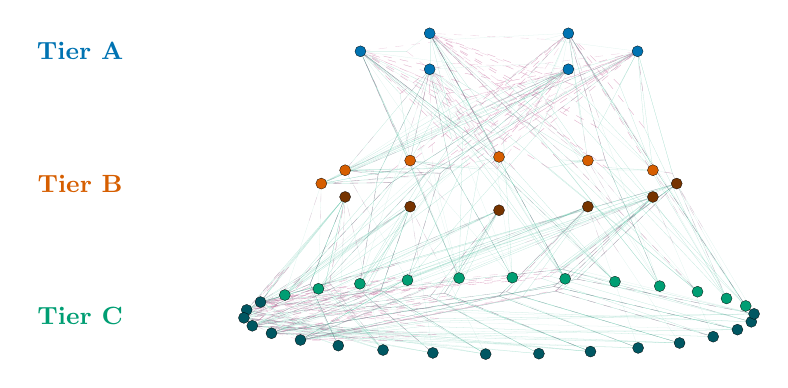
\begin{tikzpicture}[scale=1.4]
  \definecolor{slotin}{rgb}{0.000,0.620,0.450}
  \definecolor{slotout}{rgb}{0.800,0.470,0.650}
  \draw[slotin, line width=0.10pt, opacity=0.12] (1.257,1.200) -- (0.419,1.309);
  \draw[slotin, line width=0.10pt, opacity=0.12] (0.629,1.363) -- (0.419,1.309);
  \draw[slotout, line width=0.14pt, opacity=0.32, dashed] (0.419,1.309) -- (-0.629,1.363);
  \draw[slotin, line width=0.10pt, opacity=0.12] (1.257,1.200) -- (1.304,0.840);
  \draw[slotin, line width=0.10pt, opacity=0.12] (1.396,0.121) -- (1.304,0.840);
  \draw[slotout, line width=0.14pt, opacity=0.32, dashed] (1.304,0.840) -- (1.257,1.200);
  \draw[slotin, line width=0.10pt, opacity=0.12] (1.257,1.200) -- (1.094,0.895);
  \draw[slotin, line width=0.10pt, opacity=0.12] (1.396,0.121) -- (1.094,0.895);
  \draw[slotout, line width=0.14pt, opacity=0.32, dashed] (1.094,0.895) -- (0.629,1.363);
  \draw[slotin, line width=0.10pt, opacity=0.12] (1.257,1.200) -- (0.675,0.895);
  \draw[slotin, line width=0.10pt, opacity=0.12] (1.396,0.121) -- (0.675,0.895);
  \draw[slotout, line width=0.14pt, opacity=0.32, dashed] (0.675,0.895) -- (-0.629,1.363);
  \draw[slotin, line width=0.10pt, opacity=0.12] (1.257,1.200) -- (0.301,0.800);
  \draw[slotin, line width=0.10pt, opacity=0.12] (-1.612,0.000) -- (0.301,0.800);
  \draw[slotout, line width=0.14pt, opacity=0.32, dashed] (0.301,0.800) -- (1.257,1.200);
  \draw[slotin, line width=0.10pt, opacity=0.12] (1.257,1.200) -- (0.091,0.854);
  \draw[slotin, line width=0.10pt, opacity=0.12] (-1.612,0.000) -- (0.091,0.854);
  \draw[slotout, line width=0.14pt, opacity=0.32, dashed] (0.091,0.854) -- (0.629,1.363);
  \draw[slotin, line width=0.10pt, opacity=0.12] (1.257,1.200) -- (-0.665,0.082);
  \draw[slotin, line width=0.10pt, opacity=0.12] (-1.612,0.000) -- (-0.665,0.082);
  \draw[slotout, line width=0.14pt, opacity=0.32, dashed] (-0.665,0.082) -- (-1.638,-0.954);
  \draw[slotin, line width=0.10pt, opacity=0.12] (1.257,1.200) -- (1.317,0.507);
  \draw[slotin, line width=0.10pt, opacity=0.12] (2.064,-1.042) -- (1.317,0.507);
  \draw[slotout, line width=0.14pt, opacity=0.32, dashed] (1.317,0.507) -- (0.629,1.363);
  \draw[slotin, line width=0.10pt, opacity=0.12] (1.257,1.200) -- (0.898,0.507);
  \draw[slotin, line width=0.10pt, opacity=0.12] (2.064,-1.042) -- (0.898,0.507);
  \draw[slotout, line width=0.14pt, opacity=0.32, dashed] (0.898,0.507) -- (-0.629,1.363);
  \draw[slotin, line width=0.10pt, opacity=0.12] (1.257,1.200) -- (1.573,0.093);
  \draw[slotin, line width=0.10pt, opacity=0.12] (2.064,-1.042) -- (1.573,0.093);
  \draw[slotout, line width=0.14pt, opacity=0.32, dashed] (1.573,0.093) -- (1.396,0.121);
  \draw[slotin, line width=0.10pt, opacity=0.12] (1.257,1.200) -- (0.292,0.482);
  \draw[slotin, line width=0.10pt, opacity=0.12] (-1.638,-0.954) -- (0.292,0.482);
  \draw[slotout, line width=0.14pt, opacity=0.32, dashed] (0.292,0.482) -- (1.257,1.200);
  \draw[slotin, line width=0.10pt, opacity=0.12] (1.257,1.200) -- (-0.665,0.082);
  \draw[slotin, line width=0.10pt, opacity=0.12] (-1.638,-0.954) -- (-0.665,0.082);
  \draw[slotout, line width=0.14pt, opacity=0.32, dashed] (-0.665,0.082) -- (-1.612,0.000);
  \draw[slotin, line width=0.10pt, opacity=0.12] (0.629,1.363) -- (-0.419,1.309);
  \draw[slotin, line width=0.10pt, opacity=0.12] (-0.629,1.363) -- (-0.419,1.309);
  \draw[slotout, line width=0.14pt, opacity=0.32, dashed] (-0.419,1.309) -- (-1.257,1.200);
  \draw[slotin, line width=0.10pt, opacity=0.12] (0.629,1.363) -- (0.885,0.949);
  \draw[slotin, line width=0.10pt, opacity=0.12] (1.396,0.121) -- (0.885,0.949);
  \draw[slotout, line width=0.14pt, opacity=0.32, dashed] (0.885,0.949) -- (0.629,1.363);
  \draw[slotin, line width=0.10pt, opacity=0.12] (0.629,1.363) -- (1.421,0.125);
  \draw[slotin, line width=0.10pt, opacity=0.12] (1.396,0.121) -- (1.421,0.125);
  \draw[slotout, line width=0.14pt, opacity=0.32, dashed] (1.421,0.125) -- (2.238,-1.110);
  \draw[slotin, line width=0.10pt, opacity=0.12] (0.629,1.363) -- (0.688,0.979);
  \draw[slotin, line width=0.10pt, opacity=0.12] (0.806,0.209) -- (0.688,0.979);
  \draw[slotout, line width=0.14pt, opacity=0.32, dashed] (0.688,0.979) -- (0.629,1.363);
  \draw[slotin, line width=0.10pt, opacity=0.12] (0.629,1.363) -- (0.269,0.979);
  \draw[slotin, line width=0.10pt, opacity=0.12] (0.806,0.209) -- (0.269,0.979);
  \draw[slotout, line width=0.14pt, opacity=0.32, dashed] (0.269,0.979) -- (-0.629,1.363);
  \draw[slotin, line width=0.10pt, opacity=0.12] (0.629,1.363) -- (0.059,0.924);
  \draw[slotin, line width=0.10pt, opacity=0.12] (0.806,0.209) -- (0.059,0.924);
  \draw[slotout, line width=0.14pt, opacity=0.32, dashed] (0.059,0.924) -- (-1.257,1.200);
  \draw[slotin, line width=0.10pt, opacity=0.12] (0.629,1.363) -- (1.165,0.539);
  \draw[slotin, line width=0.10pt, opacity=0.12] (2.238,-1.110) -- (1.165,0.539);
  \draw[slotout, line width=0.14pt, opacity=0.32, dashed] (1.165,0.539) -- (0.629,1.363);
  \draw[slotin, line width=0.10pt, opacity=0.12] (0.629,1.363) -- (0.746,0.539);
  \draw[slotin, line width=0.10pt, opacity=0.12] (2.238,-1.110) -- (0.746,0.539);
  \draw[slotout, line width=0.14pt, opacity=0.32, dashed] (0.746,0.539) -- (-0.629,1.363);
  \draw[slotin, line width=0.10pt, opacity=0.12] (0.629,1.363) -- (1.421,0.125);
  \draw[slotin, line width=0.10pt, opacity=0.12] (2.238,-1.110) -- (1.421,0.125);
  \draw[slotout, line width=0.14pt, opacity=0.32, dashed] (1.421,0.125) -- (1.396,0.121);
  \draw[slotin, line width=0.10pt, opacity=0.12] (0.629,1.363) -- (0.486,0.599);
  \draw[slotin, line width=0.10pt, opacity=0.12] (1.458,-0.930) -- (0.486,0.599);
  \draw[slotout, line width=0.14pt, opacity=0.32, dashed] (0.486,0.599) -- (-0.629,1.363);
  \draw[slotin, line width=0.10pt, opacity=0.12] (0.629,1.363) -- (0.276,0.544);
  \draw[slotin, line width=0.10pt, opacity=0.12] (1.458,-0.930) -- (0.276,0.544);
  \draw[slotout, line width=0.14pt, opacity=0.32, dashed] (0.276,0.544) -- (-1.257,1.200);
  \draw[slotin, line width=0.10pt, opacity=0.12] (0.629,1.363) -- (0.964,0.214);
  \draw[slotin, line width=0.10pt, opacity=0.12] (1.458,-0.930) -- (0.964,0.214);
  \draw[slotout, line width=0.14pt, opacity=0.32, dashed] (0.964,0.214) -- (0.806,0.209);
  \draw[slotin, line width=0.10pt, opacity=0.12] (-0.629,1.363) -- (-0.838,1.200);
  \draw[slotin, line width=0.10pt, opacity=0.12] (-1.257,1.200) -- (-0.838,1.200);
  \draw[slotout, line width=0.14pt, opacity=0.32, dashed] (-0.838,1.200) -- (-0.629,1.037);
  \draw[slotin, line width=0.10pt, opacity=0.12] (-0.629,1.363) -- (-0.360,0.924);
  \draw[slotin, line width=0.10pt, opacity=0.12] (0.806,0.209) -- (-0.360,0.924);
  \draw[slotout, line width=0.14pt, opacity=0.32, dashed] (-0.360,0.924) -- (-1.257,1.200);
  \draw[slotin, line width=0.10pt, opacity=0.12] (-0.629,1.363) -- (0.659,0.197);
  \draw[slotin, line width=0.10pt, opacity=0.12] (0.806,0.209) -- (0.659,0.197);
  \draw[slotout, line width=0.14pt, opacity=0.32, dashed] (0.659,0.197) -- (1.801,-0.981);
  \draw[slotin, line width=0.10pt, opacity=0.12] (-0.629,1.363) -- (-0.419,0.990);
  \draw[slotin, line width=0.10pt, opacity=0.12] (0.000,0.242) -- (-0.419,0.990);
  \draw[slotout, line width=0.14pt, opacity=0.32, dashed] (-0.419,0.990) -- (-0.629,1.363);
  \draw[slotin, line width=0.10pt, opacity=0.12] (-0.629,1.363) -- (-0.419,0.881);
  \draw[slotin, line width=0.10pt, opacity=0.12] (0.000,0.242) -- (-0.419,0.881);
  \draw[slotout, line width=0.14pt, opacity=0.32, dashed] (-0.419,0.881) -- (-0.629,1.037);
  \draw[slotin, line width=0.10pt, opacity=0.12] (-0.629,1.363) -- (-0.010,0.247);
  \draw[slotin, line width=0.10pt, opacity=0.12] (0.000,0.242) -- (-0.010,0.247);
  \draw[slotout, line width=0.14pt, opacity=0.32, dashed] (-0.010,0.247) -- (0.600,-0.864);
  \draw[slotin, line width=0.10pt, opacity=0.12] (-0.629,1.363) -- (0.181,0.582);
  \draw[slotin, line width=0.10pt, opacity=0.12] (1.801,-0.981) -- (0.181,0.582);
  \draw[slotout, line width=0.14pt, opacity=0.32, dashed] (0.181,0.582) -- (-0.629,1.363);
  \draw[slotin, line width=0.10pt, opacity=0.12] (-0.629,1.363) -- (-0.028,0.527);
  \draw[slotin, line width=0.10pt, opacity=0.12] (1.801,-0.981) -- (-0.028,0.527);
  \draw[slotout, line width=0.14pt, opacity=0.32, dashed] (-0.028,0.527) -- (-1.257,1.200);
  \draw[slotin, line width=0.10pt, opacity=0.12] (-0.629,1.363) -- (-0.219,0.621);
  \draw[slotin, line width=0.10pt, opacity=0.12] (0.600,-0.864) -- (-0.219,0.621);
  \draw[slotout, line width=0.14pt, opacity=0.32, dashed] (-0.219,0.621) -- (-0.629,1.363);
  \draw[slotin, line width=0.10pt, opacity=0.12] (-0.629,1.363) -- (-0.429,0.566);
  \draw[slotin, line width=0.10pt, opacity=0.12] (0.600,-0.864) -- (-0.429,0.566);
  \draw[slotout, line width=0.14pt, opacity=0.32, dashed] (-0.429,0.566) -- (-1.257,1.200);
  \draw[slotin, line width=0.10pt, opacity=0.12] (-0.629,1.363) -- (-0.219,0.512);
  \draw[slotin, line width=0.10pt, opacity=0.12] (0.600,-0.864) -- (-0.219,0.512);
  \draw[slotout, line width=0.14pt, opacity=0.32, dashed] (-0.219,0.512) -- (-0.629,1.037);
  \draw[slotin, line width=0.10pt, opacity=0.12] (-1.257,1.200) -- (-0.419,1.091);
  \draw[slotin, line width=0.10pt, opacity=0.12] (-0.629,1.037) -- (-0.419,1.091);
  \draw[slotout, line width=0.14pt, opacity=0.32, dashed] (-0.419,1.091) -- (0.629,1.037);
  \draw[slotin, line width=0.10pt, opacity=0.12] (-1.257,1.200) -- (-0.838,0.881);
  \draw[slotin, line width=0.10pt, opacity=0.12] (0.000,0.242) -- (-0.838,0.881);
  \draw[slotout, line width=0.14pt, opacity=0.32, dashed] (-0.838,0.881) -- (-1.257,1.200);
  \draw[slotin, line width=0.10pt, opacity=0.12] (-1.257,1.200) -- (-0.629,0.826);
  \draw[slotin, line width=0.10pt, opacity=0.12] (0.000,0.242) -- (-0.629,0.826);
  \draw[slotout, line width=0.14pt, opacity=0.32, dashed] (-0.629,0.826) -- (-0.629,1.037);
  \draw[slotin, line width=0.10pt, opacity=0.12] (-1.257,1.200) -- (-1.107,0.870);
  \draw[slotin, line width=0.10pt, opacity=0.12] (-0.806,0.209) -- (-1.107,0.870);
  \draw[slotout, line width=0.14pt, opacity=0.32, dashed] (-1.107,0.870) -- (-1.257,1.200);
  \draw[slotin, line width=0.10pt, opacity=0.12] (-1.257,1.200) -- (-0.897,0.815);
  \draw[slotin, line width=0.10pt, opacity=0.12] (-0.806,0.209) -- (-0.897,0.815);
  \draw[slotout, line width=0.14pt, opacity=0.32, dashed] (-0.897,0.815) -- (-0.629,1.037);
  \draw[slotin, line width=0.10pt, opacity=0.12] (-1.257,1.200) -- (-0.478,0.815);
  \draw[slotin, line width=0.10pt, opacity=0.12] (-0.806,0.209) -- (-0.478,0.815);
  \draw[slotout, line width=0.14pt, opacity=0.32, dashed] (-0.478,0.815) -- (0.629,1.037);
  \draw[slotin, line width=0.10pt, opacity=0.12] (-1.257,1.200) -- (-0.809,0.184);
  \draw[slotin, line width=0.10pt, opacity=0.12] (-0.806,0.209) -- (-0.809,0.184);
  \draw[slotout, line width=0.14pt, opacity=0.32, dashed] (-0.809,0.184) -- (-0.362,-0.857);
  \draw[slotin, line width=0.10pt, opacity=0.12] (-1.257,1.200) -- (-0.278,0.449);
  \draw[slotin, line width=0.10pt, opacity=0.12] (1.052,-0.890) -- (-0.278,0.449);
  \draw[slotout, line width=0.14pt, opacity=0.32, dashed] (-0.278,0.449) -- (-0.629,1.037);
  \draw[slotin, line width=0.10pt, opacity=0.12] (-1.257,1.200) -- (-0.068,0.184);
  \draw[slotin, line width=0.10pt, opacity=0.12] (1.052,-0.890) -- (-0.068,0.184);
  \draw[slotout, line width=0.14pt, opacity=0.32, dashed] (-0.068,0.184) -- (0.000,0.242);
  \draw[slotin, line width=0.10pt, opacity=0.12] (-1.257,1.200) -- (-0.959,0.514);
  \draw[slotin, line width=0.10pt, opacity=0.12] (-0.362,-0.857) -- (-0.959,0.514);
  \draw[slotout, line width=0.14pt, opacity=0.32, dashed] (-0.959,0.514) -- (-1.257,1.200);
  \draw[slotin, line width=0.10pt, opacity=0.12] (-1.257,1.200) -- (-0.330,0.460);
  \draw[slotin, line width=0.10pt, opacity=0.12] (-0.362,-0.857) -- (-0.330,0.460);
  \draw[slotout, line width=0.14pt, opacity=0.32, dashed] (-0.330,0.460) -- (0.629,1.037);
  \draw[slotin, line width=0.10pt, opacity=0.12] (-1.257,1.200) -- (-0.809,0.184);
  \draw[slotin, line width=0.10pt, opacity=0.12] (-0.362,-0.857) -- (-0.809,0.184);
  \draw[slotout, line width=0.14pt, opacity=0.32, dashed] (-0.809,0.184) -- (-0.806,0.209);
  \draw[slotin, line width=0.10pt, opacity=0.12] (-0.629,1.037) -- (0.419,1.091);
  \draw[slotin, line width=0.10pt, opacity=0.12] (0.629,1.037) -- (0.419,1.091);
  \draw[slotout, line width=0.14pt, opacity=0.32, dashed] (0.419,1.091) -- (1.257,1.200);
  \draw[slotin, line width=0.10pt, opacity=0.12] (-0.629,1.037) -- (-0.688,0.761);
  \draw[slotin, line width=0.10pt, opacity=0.12] (-0.806,0.209) -- (-0.688,0.761);
  \draw[slotout, line width=0.14pt, opacity=0.32, dashed] (-0.688,0.761) -- (-0.629,1.037);
  \draw[slotin, line width=0.10pt, opacity=0.12] (-0.629,1.037) -- (-0.438,0.131);
  \draw[slotin, line width=0.10pt, opacity=0.12] (-0.806,0.209) -- (-0.438,0.131);
  \draw[slotout, line width=0.14pt, opacity=0.32, dashed] (-0.438,0.131) -- (0.121,-0.853);
  \draw[slotin, line width=0.10pt, opacity=0.12] (-0.629,1.037) -- (-0.256,0.786);
  \draw[slotin, line width=0.10pt, opacity=0.12] (-1.396,0.121) -- (-0.256,0.786);
  \draw[slotout, line width=0.14pt, opacity=0.32, dashed] (-0.256,0.786) -- (1.257,1.200);
  \draw[slotin, line width=0.10pt, opacity=0.12] (-0.629,1.037) -- (-0.885,0.731);
  \draw[slotin, line width=0.10pt, opacity=0.12] (-1.396,0.121) -- (-0.885,0.731);
  \draw[slotout, line width=0.14pt, opacity=0.32, dashed] (-0.885,0.731) -- (-0.629,1.037);
  \draw[slotin, line width=0.10pt, opacity=0.12] (-0.629,1.037) -- (-1.096,0.083);
  \draw[slotin, line width=0.10pt, opacity=0.12] (-1.396,0.121) -- (-1.096,0.083);
  \draw[slotout, line width=0.14pt, opacity=0.32, dashed] (-1.096,0.083) -- (-1.262,-0.909);
  \draw[slotin, line width=0.10pt, opacity=0.12] (-0.629,1.037) -- (-0.379,0.407);
  \draw[slotin, line width=0.10pt, opacity=0.12] (0.121,-0.853) -- (-0.379,0.407);
  \draw[slotout, line width=0.14pt, opacity=0.32, dashed] (-0.379,0.407) -- (-0.629,1.037);
  \draw[slotin, line width=0.10pt, opacity=0.12] (-0.629,1.037) -- (0.040,0.407);
  \draw[slotin, line width=0.10pt, opacity=0.12] (0.121,-0.853) -- (0.040,0.407);
  \draw[slotout, line width=0.14pt, opacity=0.32, dashed] (0.040,0.407) -- (0.629,1.037);
  \draw[slotin, line width=0.10pt, opacity=0.12] (-0.629,1.037) -- (-0.438,0.131);
  \draw[slotin, line width=0.10pt, opacity=0.12] (0.121,-0.853) -- (-0.438,0.131);
  \draw[slotout, line width=0.14pt, opacity=0.32, dashed] (-0.438,0.131) -- (-0.806,0.209);
  \draw[slotin, line width=0.10pt, opacity=0.12] (-0.629,1.037) -- (-0.840,0.388);
  \draw[slotin, line width=0.10pt, opacity=0.12] (-1.262,-0.909) -- (-0.840,0.388);
  \draw[slotout, line width=0.14pt, opacity=0.32, dashed] (-0.840,0.388) -- (-0.629,1.037);
  \draw[slotin, line width=0.10pt, opacity=0.12] (-0.629,1.037) -- (-0.421,0.388);
  \draw[slotin, line width=0.10pt, opacity=0.12] (-1.262,-0.909) -- (-0.421,0.388);
  \draw[slotout, line width=0.14pt, opacity=0.32, dashed] (-0.421,0.388) -- (0.629,1.037);
  \draw[slotin, line width=0.10pt, opacity=0.12] (-0.629,1.037) -- (-1.096,0.083);
  \draw[slotin, line width=0.10pt, opacity=0.12] (-1.262,-0.909) -- (-1.096,0.083);
  \draw[slotout, line width=0.14pt, opacity=0.32, dashed] (-1.096,0.083) -- (-1.396,0.121);
  \draw[slotin, line width=0.10pt, opacity=0.12] (0.629,1.037) -- (0.163,0.786);
  \draw[slotin, line width=0.10pt, opacity=0.12] (-1.396,0.121) -- (0.163,0.786);
  \draw[slotout, line width=0.14pt, opacity=0.32, dashed] (0.163,0.786) -- (1.257,1.200);
  \draw[slotin, line width=0.10pt, opacity=0.12] (0.629,1.037) -- (-0.046,0.731);
  \draw[slotin, line width=0.10pt, opacity=0.12] (-1.396,0.121) -- (-0.046,0.731);
  \draw[slotout, line width=0.14pt, opacity=0.32, dashed] (-0.046,0.731) -- (0.629,1.037);
  \draw[slotin, line width=0.10pt, opacity=0.12] (0.629,1.037) -- (-0.533,0.094);
  \draw[slotin, line width=0.10pt, opacity=0.12] (-1.396,0.121) -- (-0.533,0.094);
  \draw[slotout, line width=0.14pt, opacity=0.32, dashed] (-0.533,0.094) -- (-0.830,-0.876);
  \draw[slotin, line width=0.10pt, opacity=0.12] (0.629,1.037) -- (0.091,0.746);
  \draw[slotin, line width=0.10pt, opacity=0.12] (-1.612,0.000) -- (0.091,0.746);
  \draw[slotout, line width=0.14pt, opacity=0.32, dashed] (0.091,0.746) -- (1.257,1.200);
  \draw[slotin, line width=0.10pt, opacity=0.12] (0.629,1.037) -- (-0.118,0.691);
  \draw[slotin, line width=0.10pt, opacity=0.12] (-1.612,0.000) -- (-0.118,0.691);
  \draw[slotout, line width=0.14pt, opacity=0.32, dashed] (-0.118,0.691) -- (0.629,1.037);
  \draw[slotin, line width=0.10pt, opacity=0.12] (0.629,1.037) -- (-0.976,0.009);
  \draw[slotin, line width=0.10pt, opacity=0.12] (-1.612,0.000) -- (-0.976,0.009);
  \draw[slotout, line width=0.14pt, opacity=0.32, dashed] (-0.976,0.009) -- (-1.943,-1.011);
  \draw[slotin, line width=0.10pt, opacity=0.12] (0.629,1.037) -- (0.352,0.454);
  \draw[slotin, line width=0.10pt, opacity=0.12] (-0.830,-0.876) -- (0.352,0.454);
  \draw[slotout, line width=0.14pt, opacity=0.32, dashed] (0.352,0.454) -- (1.257,1.200);
  \draw[slotin, line width=0.10pt, opacity=0.12] (0.629,1.037) -- (-0.533,0.094);
  \draw[slotin, line width=0.10pt, opacity=0.12] (-0.830,-0.876) -- (-0.533,0.094);
  \draw[slotout, line width=0.14pt, opacity=0.32, dashed] (-0.533,0.094) -- (-1.396,0.121);
  \draw[slotin, line width=0.10pt, opacity=0.12] (0.629,1.037) -- (-0.019,0.409);
  \draw[slotin, line width=0.10pt, opacity=0.12] (-1.943,-1.011) -- (-0.019,0.409);
  \draw[slotout, line width=0.14pt, opacity=0.32, dashed] (-0.019,0.409) -- (1.257,1.200);
  \draw[slotin, line width=0.10pt, opacity=0.12] (0.629,1.037) -- (-0.229,0.463);
  \draw[slotin, line width=0.10pt, opacity=0.12] (-1.943,-1.011) -- (-0.229,0.463);
  \draw[slotout, line width=0.14pt, opacity=0.32, dashed] (-0.229,0.463) -- (0.629,1.363);
  \draw[slotin, line width=0.10pt, opacity=0.12] (0.629,1.037) -- (-0.976,0.009);
  \draw[slotin, line width=0.10pt, opacity=0.12] (-1.943,-1.011) -- (-0.976,0.009);
  \draw[slotout, line width=0.14pt, opacity=0.32, dashed] (-0.976,0.009) -- (-1.612,0.000);
  \draw[slotin, line width=0.10pt, opacity=0.12] (1.396,0.121) -- (1.304,0.840);
  \draw[slotin, line width=0.10pt, opacity=0.12] (1.257,1.200) -- (1.304,0.840);
  \draw[slotout, line width=0.14pt, opacity=0.32, dashed] (1.304,0.840) -- (1.257,1.200);
  \draw[slotin, line width=0.10pt, opacity=0.12] (1.396,0.121) -- (1.094,0.895);
  \draw[slotin, line width=0.10pt, opacity=0.12] (1.257,1.200) -- (1.094,0.895);
  \draw[slotout, line width=0.14pt, opacity=0.32, dashed] (1.094,0.895) -- (0.629,1.363);
  \draw[slotin, line width=0.10pt, opacity=0.12] (1.396,0.121) -- (0.675,0.895);
  \draw[slotin, line width=0.10pt, opacity=0.12] (1.257,1.200) -- (0.675,0.895);
  \draw[slotout, line width=0.14pt, opacity=0.32, dashed] (0.675,0.895) -- (-0.629,1.363);
  \draw[slotin, line width=0.10pt, opacity=0.12] (1.396,0.121) -- (1.573,0.093);
  \draw[slotin, line width=0.10pt, opacity=0.12] (1.257,1.200) -- (1.573,0.093);
  \draw[slotout, line width=0.14pt, opacity=0.32, dashed] (1.573,0.093) -- (2.064,-1.042);
  \draw[slotin, line width=0.10pt, opacity=0.12] (1.396,0.121) -- (0.885,0.949);
  \draw[slotin, line width=0.10pt, opacity=0.12] (0.629,1.363) -- (0.885,0.949);
  \draw[slotout, line width=0.14pt, opacity=0.32, dashed] (0.885,0.949) -- (0.629,1.363);
  \draw[slotin, line width=0.10pt, opacity=0.12] (1.396,0.121) -- (0.465,0.949);
  \draw[slotin, line width=0.10pt, opacity=0.12] (0.629,1.363) -- (0.465,0.949);
  \draw[slotout, line width=0.14pt, opacity=0.32, dashed] (0.465,0.949) -- (-0.629,1.363);
  \draw[slotin, line width=0.10pt, opacity=0.12] (1.396,0.121) -- (1.421,0.125);
  \draw[slotin, line width=0.10pt, opacity=0.12] (0.629,1.363) -- (1.421,0.125);
  \draw[slotout, line width=0.14pt, opacity=0.32, dashed] (1.421,0.125) -- (2.238,-1.110);
  \draw[slotin, line width=0.10pt, opacity=0.12] (1.396,0.121) -- (1.421,0.125);
  \draw[slotin, line width=0.10pt, opacity=0.12] (2.238,-1.110) -- (1.421,0.125);
  \draw[slotout, line width=0.14pt, opacity=0.32, dashed] (1.421,0.125) -- (0.629,1.363);
  \draw[slotin, line width=0.10pt, opacity=0.12] (1.396,0.121) -- (1.002,0.125);
  \draw[slotin, line width=0.10pt, opacity=0.12] (2.238,-1.110) -- (1.002,0.125);
  \draw[slotout, line width=0.14pt, opacity=0.32, dashed] (1.002,0.125) -- (-0.629,1.363);
  \draw[slotin, line width=0.10pt, opacity=0.12] (1.396,0.121) -- (1.677,-0.289);
  \draw[slotin, line width=0.10pt, opacity=0.12] (2.238,-1.110) -- (1.677,-0.289);
  \draw[slotout, line width=0.14pt, opacity=0.32, dashed] (1.677,-0.289) -- (1.396,0.121);
  \draw[slotin, line width=0.10pt, opacity=0.12] (1.396,0.121) -- (1.363,0.147);
  \draw[slotin, line width=0.10pt, opacity=0.12] (2.064,-1.042) -- (1.363,0.147);
  \draw[slotout, line width=0.14pt, opacity=0.32, dashed] (1.363,0.147) -- (0.629,1.363);
  \draw[slotin, line width=0.10pt, opacity=0.12] (1.396,0.121) -- (0.944,0.147);
  \draw[slotin, line width=0.10pt, opacity=0.12] (2.064,-1.042) -- (0.944,0.147);
  \draw[slotout, line width=0.14pt, opacity=0.32, dashed] (0.944,0.147) -- (-0.629,1.363);
  \draw[slotin, line width=0.10pt, opacity=0.12] (1.396,0.121) -- (1.619,-0.267);
  \draw[slotin, line width=0.10pt, opacity=0.12] (2.064,-1.042) -- (1.619,-0.267);
  \draw[slotout, line width=0.14pt, opacity=0.32, dashed] (1.619,-0.267) -- (1.396,0.121);
  \draw[slotin, line width=0.10pt, opacity=0.12] (0.806,0.209) -- (0.269,0.979);
  \draw[slotin, line width=0.10pt, opacity=0.12] (0.629,1.363) -- (0.269,0.979);
  \draw[slotout, line width=0.14pt, opacity=0.32, dashed] (0.269,0.979) -- (-0.629,1.363);
  \draw[slotin, line width=0.10pt, opacity=0.12] (0.806,0.209) -- (0.059,0.924);
  \draw[slotin, line width=0.10pt, opacity=0.12] (0.629,1.363) -- (0.059,0.924);
  \draw[slotout, line width=0.14pt, opacity=0.32, dashed] (0.059,0.924) -- (-1.257,1.200);
  \draw[slotin, line width=0.10pt, opacity=0.12] (0.806,0.209) -- (0.747,0.594);
  \draw[slotin, line width=0.10pt, opacity=0.12] (0.629,1.363) -- (0.747,0.594);
  \draw[slotout, line width=0.14pt, opacity=0.32, dashed] (0.747,0.594) -- (0.806,0.209);
  \draw[slotin, line width=0.10pt, opacity=0.12] (0.806,0.209) -- (0.964,0.214);
  \draw[slotin, line width=0.10pt, opacity=0.12] (0.629,1.363) -- (0.964,0.214);
  \draw[slotout, line width=0.14pt, opacity=0.32, dashed] (0.964,0.214) -- (1.458,-0.930);
  \draw[slotin, line width=0.10pt, opacity=0.12] (0.806,0.209) -- (-0.360,0.924);
  \draw[slotin, line width=0.10pt, opacity=0.12] (-0.629,1.363) -- (-0.360,0.924);
  \draw[slotout, line width=0.14pt, opacity=0.32, dashed] (-0.360,0.924) -- (-1.257,1.200);
  \draw[slotin, line width=0.10pt, opacity=0.12] (0.806,0.209) -- (0.328,0.594);
  \draw[slotin, line width=0.10pt, opacity=0.12] (-0.629,1.363) -- (0.328,0.594);
  \draw[slotout, line width=0.14pt, opacity=0.32, dashed] (0.328,0.594) -- (0.806,0.209);
  \draw[slotin, line width=0.10pt, opacity=0.12] (0.806,0.209) -- (0.659,0.197);
  \draw[slotin, line width=0.10pt, opacity=0.12] (-0.629,1.363) -- (0.659,0.197);
  \draw[slotout, line width=0.14pt, opacity=0.32, dashed] (0.659,0.197) -- (1.801,-0.981);
  \draw[slotin, line width=0.10pt, opacity=0.12] (0.806,0.209) -- (0.450,0.143);
  \draw[slotin, line width=0.10pt, opacity=0.12] (1.801,-0.981) -- (0.450,0.143);
  \draw[slotout, line width=0.14pt, opacity=0.32, dashed] (0.450,0.143) -- (-1.257,1.200);
  \draw[slotin, line width=0.10pt, opacity=0.12] (0.806,0.209) -- (1.138,-0.187);
  \draw[slotin, line width=0.10pt, opacity=0.12] (1.801,-0.981) -- (1.138,-0.187);
  \draw[slotout, line width=0.14pt, opacity=0.32, dashed] (1.138,-0.187) -- (0.806,0.209);
  \draw[slotin, line width=0.10pt, opacity=0.12] (0.806,0.209) -- (0.964,0.214);
  \draw[slotin, line width=0.10pt, opacity=0.12] (1.458,-0.930) -- (0.964,0.214);
  \draw[slotout, line width=0.14pt, opacity=0.32, dashed] (0.964,0.214) -- (0.629,1.363);
  \draw[slotin, line width=0.10pt, opacity=0.12] (0.806,0.209) -- (0.545,0.214);
  \draw[slotin, line width=0.10pt, opacity=0.12] (1.458,-0.930) -- (0.545,0.214);
  \draw[slotout, line width=0.14pt, opacity=0.32, dashed] (0.545,0.214) -- (-0.629,1.363);
  \draw[slotin, line width=0.10pt, opacity=0.12] (0.806,0.209) -- (1.024,-0.170);
  \draw[slotin, line width=0.10pt, opacity=0.12] (1.458,-0.930) -- (1.024,-0.170);
  \draw[slotout, line width=0.14pt, opacity=0.32, dashed] (1.024,-0.170) -- (0.806,0.209);
  \draw[slotin, line width=0.10pt, opacity=0.12] (0.000,0.242) -- (-0.419,0.990);
  \draw[slotin, line width=0.10pt, opacity=0.12] (-0.629,1.363) -- (-0.419,0.990);
  \draw[slotout, line width=0.14pt, opacity=0.32, dashed] (-0.419,0.990) -- (-0.629,1.363);
  \draw[slotin, line width=0.10pt, opacity=0.12] (0.000,0.242) -- (-0.629,0.935);
  \draw[slotin, line width=0.10pt, opacity=0.12] (-0.629,1.363) -- (-0.629,0.935);
  \draw[slotout, line width=0.14pt, opacity=0.32, dashed] (-0.629,0.935) -- (-1.257,1.200);
  \draw[slotin, line width=0.10pt, opacity=0.12] (0.000,0.242) -- (-0.210,0.616);
  \draw[slotin, line width=0.10pt, opacity=0.12] (-0.629,1.363) -- (-0.210,0.616);
  \draw[slotout, line width=0.14pt, opacity=0.32, dashed] (-0.210,0.616) -- (0.000,0.242);
  \draw[slotin, line width=0.10pt, opacity=0.12] (0.000,0.242) -- (-0.010,0.247);
  \draw[slotin, line width=0.10pt, opacity=0.12] (-0.629,1.363) -- (-0.010,0.247);
  \draw[slotout, line width=0.14pt, opacity=0.32, dashed] (-0.010,0.247) -- (0.600,-0.864);
  \draw[slotin, line width=0.10pt, opacity=0.12] (0.000,0.242) -- (-0.838,0.881);
  \draw[slotin, line width=0.10pt, opacity=0.12] (-1.257,1.200) -- (-0.838,0.881);
  \draw[slotout, line width=0.14pt, opacity=0.32, dashed] (-0.838,0.881) -- (-1.257,1.200);
  \draw[slotin, line width=0.10pt, opacity=0.12] (0.000,0.242) -- (-0.419,0.561);
  \draw[slotin, line width=0.10pt, opacity=0.12] (-1.257,1.200) -- (-0.419,0.561);
  \draw[slotout, line width=0.14pt, opacity=0.32, dashed] (-0.419,0.561) -- (0.000,0.242);
  \draw[slotin, line width=0.10pt, opacity=0.12] (0.000,0.242) -- (-0.068,0.184);
  \draw[slotin, line width=0.10pt, opacity=0.12] (-1.257,1.200) -- (-0.068,0.184);
  \draw[slotout, line width=0.14pt, opacity=0.32, dashed] (-0.068,0.184) -- (1.052,-0.890);
  \draw[slotin, line width=0.10pt, opacity=0.12] (0.000,0.242) -- (-0.068,0.184);
  \draw[slotin, line width=0.10pt, opacity=0.12] (1.052,-0.890) -- (-0.068,0.184);
  \draw[slotout, line width=0.14pt, opacity=0.32, dashed] (-0.068,0.184) -- (-1.257,1.200);
  \draw[slotin, line width=0.10pt, opacity=0.12] (0.000,0.242) -- (0.141,0.129);
  \draw[slotin, line width=0.10pt, opacity=0.12] (1.052,-0.890) -- (0.141,0.129);
  \draw[slotout, line width=0.14pt, opacity=0.32, dashed] (0.141,0.129) -- (-0.629,1.037);
  \draw[slotin, line width=0.10pt, opacity=0.12] (0.000,0.242) -- (-0.010,0.247);
  \draw[slotin, line width=0.10pt, opacity=0.12] (0.600,-0.864) -- (-0.010,0.247);
  \draw[slotout, line width=0.14pt, opacity=0.32, dashed] (-0.010,0.247) -- (-0.629,1.363);
  \draw[slotin, line width=0.10pt, opacity=0.12] (0.000,0.242) -- (-0.219,0.193);
  \draw[slotin, line width=0.10pt, opacity=0.12] (0.600,-0.864) -- (-0.219,0.193);
  \draw[slotout, line width=0.14pt, opacity=0.32, dashed] (-0.219,0.193) -- (-1.257,1.200);
  \draw[slotin, line width=0.10pt, opacity=0.12] (0.000,0.242) -- (-0.010,0.138);
  \draw[slotin, line width=0.10pt, opacity=0.12] (0.600,-0.864) -- (-0.010,0.138);
  \draw[slotout, line width=0.14pt, opacity=0.32, dashed] (-0.010,0.138) -- (-0.629,1.037);
  \draw[slotin, line width=0.10pt, opacity=0.12] (-0.806,0.209) -- (-1.107,0.870);
  \draw[slotin, line width=0.10pt, opacity=0.12] (-1.257,1.200) -- (-1.107,0.870);
  \draw[slotout, line width=0.14pt, opacity=0.32, dashed] (-1.107,0.870) -- (-1.257,1.200);
  \draw[slotin, line width=0.10pt, opacity=0.12] (-0.806,0.209) -- (-0.897,0.815);
  \draw[slotin, line width=0.10pt, opacity=0.12] (-1.257,1.200) -- (-0.897,0.815);
  \draw[slotout, line width=0.14pt, opacity=0.32, dashed] (-0.897,0.815) -- (-0.629,1.037);
  \draw[slotin, line width=0.10pt, opacity=0.12] (-0.806,0.209) -- (-0.478,0.815);
  \draw[slotin, line width=0.10pt, opacity=0.12] (-1.257,1.200) -- (-0.478,0.815);
  \draw[slotout, line width=0.14pt, opacity=0.32, dashed] (-0.478,0.815) -- (0.629,1.037);
  \draw[slotin, line width=0.10pt, opacity=0.12] (-0.806,0.209) -- (-0.957,0.540);
  \draw[slotin, line width=0.10pt, opacity=0.12] (-1.257,1.200) -- (-0.957,0.540);
  \draw[slotout, line width=0.14pt, opacity=0.32, dashed] (-0.957,0.540) -- (-0.806,0.209);
  \draw[slotin, line width=0.10pt, opacity=0.12] (-0.806,0.209) -- (-0.688,0.761);
  \draw[slotin, line width=0.10pt, opacity=0.12] (-0.629,1.037) -- (-0.688,0.761);
  \draw[slotout, line width=0.14pt, opacity=0.32, dashed] (-0.688,0.761) -- (-0.629,1.037);
  \draw[slotin, line width=0.10pt, opacity=0.12] (-0.806,0.209) -- (-0.269,0.761);
  \draw[slotin, line width=0.10pt, opacity=0.12] (-0.629,1.037) -- (-0.269,0.761);
  \draw[slotout, line width=0.14pt, opacity=0.32, dashed] (-0.269,0.761) -- (0.629,1.037);
  \draw[slotin, line width=0.10pt, opacity=0.12] (-0.806,0.209) -- (-0.747,0.485);
  \draw[slotin, line width=0.10pt, opacity=0.12] (-0.629,1.037) -- (-0.747,0.485);
  \draw[slotout, line width=0.14pt, opacity=0.32, dashed] (-0.747,0.485) -- (-0.806,0.209);
  \draw[slotin, line width=0.10pt, opacity=0.12] (-0.806,0.209) -- (-0.438,0.131);
  \draw[slotin, line width=0.10pt, opacity=0.12] (0.121,-0.853) -- (-0.438,0.131);
  \draw[slotout, line width=0.14pt, opacity=0.32, dashed] (-0.438,0.131) -- (-0.629,1.037);
  \draw[slotin, line width=0.10pt, opacity=0.12] (-0.806,0.209) -- (-0.019,0.131);
  \draw[slotin, line width=0.10pt, opacity=0.12] (0.121,-0.853) -- (-0.019,0.131);
  \draw[slotout, line width=0.14pt, opacity=0.32, dashed] (-0.019,0.131) -- (0.629,1.037);
  \draw[slotin, line width=0.10pt, opacity=0.12] (-0.806,0.209) -- (-0.497,-0.145);
  \draw[slotin, line width=0.10pt, opacity=0.12] (0.121,-0.853) -- (-0.497,-0.145);
  \draw[slotout, line width=0.14pt, opacity=0.32, dashed] (-0.497,-0.145) -- (-0.806,0.209);
  \draw[slotin, line width=0.10pt, opacity=0.12] (-0.806,0.209) -- (-0.809,0.184);
  \draw[slotin, line width=0.10pt, opacity=0.12] (-0.362,-0.857) -- (-0.809,0.184);
  \draw[slotout, line width=0.14pt, opacity=0.32, dashed] (-0.809,0.184) -- (-1.257,1.200);
  \draw[slotin, line width=0.10pt, opacity=0.12] (-0.806,0.209) -- (-0.180,0.130);
  \draw[slotin, line width=0.10pt, opacity=0.12] (-0.362,-0.857) -- (-0.180,0.130);
  \draw[slotout, line width=0.14pt, opacity=0.32, dashed] (-0.180,0.130) -- (0.629,1.037);
  \draw[slotin, line width=0.10pt, opacity=0.12] (-0.806,0.209) -- (-0.658,-0.146);
  \draw[slotin, line width=0.10pt, opacity=0.12] (-0.362,-0.857) -- (-0.658,-0.146);
  \draw[slotout, line width=0.14pt, opacity=0.32, dashed] (-0.658,-0.146) -- (-0.806,0.209);
  \draw[slotin, line width=0.10pt, opacity=0.12] (-1.396,0.121) -- (-0.256,0.786);
  \draw[slotin, line width=0.10pt, opacity=0.12] (-0.629,1.037) -- (-0.256,0.786);
  \draw[slotout, line width=0.14pt, opacity=0.32, dashed] (-0.256,0.786) -- (1.257,1.200);
  \draw[slotin, line width=0.10pt, opacity=0.12] (-1.396,0.121) -- (-0.465,0.731);
  \draw[slotin, line width=0.10pt, opacity=0.12] (-0.629,1.037) -- (-0.465,0.731);
  \draw[slotout, line width=0.14pt, opacity=0.32, dashed] (-0.465,0.731) -- (0.629,1.037);
  \draw[slotin, line width=0.10pt, opacity=0.12] (-1.396,0.121) -- (-1.140,0.426);
  \draw[slotin, line width=0.10pt, opacity=0.12] (-0.629,1.037) -- (-1.140,0.426);
  \draw[slotout, line width=0.14pt, opacity=0.32, dashed] (-1.140,0.426) -- (-1.396,0.121);
  \draw[slotin, line width=0.10pt, opacity=0.12] (-1.396,0.121) -- (-1.096,0.083);
  \draw[slotin, line width=0.10pt, opacity=0.12] (-0.629,1.037) -- (-1.096,0.083);
  \draw[slotout, line width=0.14pt, opacity=0.32, dashed] (-1.096,0.083) -- (-1.262,-0.909);
  \draw[slotin, line width=0.10pt, opacity=0.12] (-1.396,0.121) -- (0.163,0.786);
  \draw[slotin, line width=0.10pt, opacity=0.12] (0.629,1.037) -- (0.163,0.786);
  \draw[slotout, line width=0.14pt, opacity=0.32, dashed] (0.163,0.786) -- (1.257,1.200);
  \draw[slotin, line width=0.10pt, opacity=0.12] (-1.396,0.121) -- (-0.721,0.426);
  \draw[slotin, line width=0.10pt, opacity=0.12] (0.629,1.037) -- (-0.721,0.426);
  \draw[slotout, line width=0.14pt, opacity=0.32, dashed] (-0.721,0.426) -- (-1.396,0.121);
  \draw[slotin, line width=0.10pt, opacity=0.12] (-1.396,0.121) -- (-0.533,0.094);
  \draw[slotin, line width=0.10pt, opacity=0.12] (0.629,1.037) -- (-0.533,0.094);
  \draw[slotout, line width=0.14pt, opacity=0.32, dashed] (-0.533,0.094) -- (-0.830,-0.876);
  \draw[slotin, line width=0.10pt, opacity=0.12] (-1.396,0.121) -- (-0.323,0.148);
  \draw[slotin, line width=0.10pt, opacity=0.12] (-0.830,-0.876) -- (-0.323,0.148);
  \draw[slotout, line width=0.14pt, opacity=0.32, dashed] (-0.323,0.148) -- (1.257,1.200);
  \draw[slotin, line width=0.10pt, opacity=0.12] (-1.396,0.121) -- (-1.208,-0.211);
  \draw[slotin, line width=0.10pt, opacity=0.12] (-0.830,-0.876) -- (-1.208,-0.211);
  \draw[slotout, line width=0.14pt, opacity=0.32, dashed] (-1.208,-0.211) -- (-1.396,0.121);
  \draw[slotin, line width=0.10pt, opacity=0.12] (-1.396,0.121) -- (-0.467,0.137);
  \draw[slotin, line width=0.10pt, opacity=0.12] (-1.262,-0.909) -- (-0.467,0.137);
  \draw[slotout, line width=0.14pt, opacity=0.32, dashed] (-0.467,0.137) -- (1.257,1.200);
  \draw[slotin, line width=0.10pt, opacity=0.12] (-1.396,0.121) -- (-1.096,0.083);
  \draw[slotin, line width=0.10pt, opacity=0.12] (-1.262,-0.909) -- (-1.096,0.083);
  \draw[slotout, line width=0.14pt, opacity=0.32, dashed] (-1.096,0.083) -- (-0.629,1.037);
  \draw[slotin, line width=0.10pt, opacity=0.12] (-1.396,0.121) -- (-0.677,0.083);
  \draw[slotin, line width=0.10pt, opacity=0.12] (-1.262,-0.909) -- (-0.677,0.083);
  \draw[slotout, line width=0.14pt, opacity=0.32, dashed] (-0.677,0.083) -- (0.629,1.037);
  \draw[slotin, line width=0.10pt, opacity=0.12] (-1.612,0.000) -- (0.301,0.800);
  \draw[slotin, line width=0.10pt, opacity=0.12] (1.257,1.200) -- (0.301,0.800);
  \draw[slotout, line width=0.14pt, opacity=0.32, dashed] (0.301,0.800) -- (1.257,1.200);
  \draw[slotin, line width=0.10pt, opacity=0.12] (-1.612,0.000) -- (0.091,0.854);
  \draw[slotin, line width=0.10pt, opacity=0.12] (1.257,1.200) -- (0.091,0.854);
  \draw[slotout, line width=0.14pt, opacity=0.32, dashed] (0.091,0.854) -- (0.629,1.363);
  \draw[slotin, line width=0.10pt, opacity=0.12] (-1.612,0.000) -- (-0.656,0.400);
  \draw[slotin, line width=0.10pt, opacity=0.12] (1.257,1.200) -- (-0.656,0.400);
  \draw[slotout, line width=0.14pt, opacity=0.32, dashed] (-0.656,0.400) -- (-1.612,0.000);
  \draw[slotin, line width=0.10pt, opacity=0.12] (-1.612,0.000) -- (0.091,0.746);
  \draw[slotin, line width=0.10pt, opacity=0.12] (0.629,1.037) -- (0.091,0.746);
  \draw[slotout, line width=0.14pt, opacity=0.32, dashed] (0.091,0.746) -- (1.257,1.200);
  \draw[slotin, line width=0.10pt, opacity=0.12] (-1.612,0.000) -- (-0.118,0.800);
  \draw[slotin, line width=0.10pt, opacity=0.12] (0.629,1.037) -- (-0.118,0.800);
  \draw[slotout, line width=0.14pt, opacity=0.32, dashed] (-0.118,0.800) -- (0.629,1.363);
  \draw[slotin, line width=0.10pt, opacity=0.12] (-1.612,0.000) -- (-0.118,0.691);
  \draw[slotin, line width=0.10pt, opacity=0.12] (0.629,1.037) -- (-0.118,0.691);
  \draw[slotout, line width=0.14pt, opacity=0.32, dashed] (-0.118,0.691) -- (0.629,1.037);
  \draw[slotin, line width=0.10pt, opacity=0.12] (-1.612,0.000) -- (-0.976,0.009);
  \draw[slotin, line width=0.10pt, opacity=0.12] (0.629,1.037) -- (-0.976,0.009);
  \draw[slotout, line width=0.14pt, opacity=0.32, dashed] (-0.976,0.009) -- (-1.943,-1.011);
  \draw[slotin, line width=0.10pt, opacity=0.12] (-1.612,0.000) -- (-0.665,0.082);
  \draw[slotin, line width=0.10pt, opacity=0.12] (-1.638,-0.954) -- (-0.665,0.082);
  \draw[slotout, line width=0.14pt, opacity=0.32, dashed] (-0.665,0.082) -- (1.257,1.200);
  \draw[slotin, line width=0.10pt, opacity=0.12] (-1.612,0.000) -- (-0.874,0.136);
  \draw[slotin, line width=0.10pt, opacity=0.12] (-1.638,-0.954) -- (-0.874,0.136);
  \draw[slotout, line width=0.14pt, opacity=0.32, dashed] (-0.874,0.136) -- (0.629,1.363);
  \draw[slotin, line width=0.10pt, opacity=0.12] (-1.612,0.000) -- (-1.621,-0.318);
  \draw[slotin, line width=0.10pt, opacity=0.12] (-1.638,-0.954) -- (-1.621,-0.318);
  \draw[slotout, line width=0.14pt, opacity=0.32, dashed] (-1.621,-0.318) -- (-1.612,0.000);
  \draw[slotin, line width=0.10pt, opacity=0.12] (-1.612,0.000) -- (-0.976,0.118);
  \draw[slotin, line width=0.10pt, opacity=0.12] (-1.943,-1.011) -- (-0.976,0.118);
  \draw[slotout, line width=0.14pt, opacity=0.32, dashed] (-0.976,0.118) -- (0.629,1.363);
  \draw[slotin, line width=0.10pt, opacity=0.12] (-1.612,0.000) -- (-0.976,0.009);
  \draw[slotin, line width=0.10pt, opacity=0.12] (-1.943,-1.011) -- (-0.976,0.009);
  \draw[slotout, line width=0.14pt, opacity=0.32, dashed] (-0.976,0.009) -- (0.629,1.037);
  \draw[slotin, line width=0.10pt, opacity=0.12] (-1.612,0.000) -- (-1.723,-0.337);
  \draw[slotin, line width=0.10pt, opacity=0.12] (-1.943,-1.011) -- (-1.723,-0.337);
  \draw[slotout, line width=0.14pt, opacity=0.32, dashed] (-1.723,-0.337) -- (-1.612,0.000);
  \draw[slotin, line width=0.10pt, opacity=0.12] (2.238,-1.110) -- (0.746,0.539);
  \draw[slotin, line width=0.10pt, opacity=0.12] (0.629,1.363) -- (0.746,0.539);
  \draw[slotout, line width=0.14pt, opacity=0.32, dashed] (0.746,0.539) -- (-0.629,1.363);
  \draw[slotin, line width=0.10pt, opacity=0.12] (2.238,-1.110) -- (1.421,0.125);
  \draw[slotin, line width=0.10pt, opacity=0.12] (0.629,1.363) -- (1.421,0.125);
  \draw[slotout, line width=0.14pt, opacity=0.32, dashed] (1.421,0.125) -- (1.396,0.121);
  \draw[slotin, line width=0.10pt, opacity=0.12] (2.238,-1.110) -- (1.421,0.125);
  \draw[slotin, line width=0.10pt, opacity=0.12] (1.396,0.121) -- (1.421,0.125);
  \draw[slotout, line width=0.14pt, opacity=0.32, dashed] (1.421,0.125) -- (0.629,1.363);
  \draw[slotin, line width=0.10pt, opacity=0.12] (2.238,-1.110) -- (1.002,0.125);
  \draw[slotin, line width=0.10pt, opacity=0.12] (1.396,0.121) -- (1.002,0.125);
  \draw[slotout, line width=0.14pt, opacity=0.32, dashed] (1.002,0.125) -- (-0.629,1.363);
  \draw[slotin, line width=0.10pt, opacity=0.12] (2.064,-1.042) -- (1.317,0.507);
  \draw[slotin, line width=0.10pt, opacity=0.12] (1.257,1.200) -- (1.317,0.507);
  \draw[slotout, line width=0.14pt, opacity=0.32, dashed] (1.317,0.507) -- (0.629,1.363);
  \draw[slotin, line width=0.10pt, opacity=0.12] (2.064,-1.042) -- (0.898,0.507);
  \draw[slotin, line width=0.10pt, opacity=0.12] (1.257,1.200) -- (0.898,0.507);
  \draw[slotout, line width=0.14pt, opacity=0.32, dashed] (0.898,0.507) -- (-0.629,1.363);
  \draw[slotin, line width=0.10pt, opacity=0.12] (2.064,-1.042) -- (1.573,0.093);
  \draw[slotin, line width=0.10pt, opacity=0.12] (1.257,1.200) -- (1.573,0.093);
  \draw[slotout, line width=0.14pt, opacity=0.32, dashed] (1.573,0.093) -- (1.396,0.121);
  \draw[slotin, line width=0.10pt, opacity=0.12] (2.064,-1.042) -- (1.363,0.147);
  \draw[slotin, line width=0.10pt, opacity=0.12] (1.396,0.121) -- (1.363,0.147);
  \draw[slotout, line width=0.14pt, opacity=0.32, dashed] (1.363,0.147) -- (0.629,1.363);
  \draw[slotin, line width=0.10pt, opacity=0.12] (2.064,-1.042) -- (0.944,0.147);
  \draw[slotin, line width=0.10pt, opacity=0.12] (1.396,0.121) -- (0.944,0.147);
  \draw[slotout, line width=0.14pt, opacity=0.32, dashed] (0.944,0.147) -- (-0.629,1.363);
  \draw[slotin, line width=0.10pt, opacity=0.12] (1.801,-0.981) -- (0.181,0.582);
  \draw[slotin, line width=0.10pt, opacity=0.12] (-0.629,1.363) -- (0.181,0.582);
  \draw[slotout, line width=0.14pt, opacity=0.32, dashed] (0.181,0.582) -- (-0.629,1.363);
  \draw[slotin, line width=0.10pt, opacity=0.12] (1.801,-0.981) -- (-0.028,0.527);
  \draw[slotin, line width=0.10pt, opacity=0.12] (-0.629,1.363) -- (-0.028,0.527);
  \draw[slotout, line width=0.14pt, opacity=0.32, dashed] (-0.028,0.527) -- (-1.257,1.200);
  \draw[slotin, line width=0.10pt, opacity=0.12] (1.801,-0.981) -- (0.659,0.197);
  \draw[slotin, line width=0.10pt, opacity=0.12] (0.806,0.209) -- (0.659,0.197);
  \draw[slotout, line width=0.14pt, opacity=0.32, dashed] (0.659,0.197) -- (-0.629,1.363);
  \draw[slotin, line width=0.10pt, opacity=0.12] (1.801,-0.981) -- (0.450,0.143);
  \draw[slotin, line width=0.10pt, opacity=0.12] (0.806,0.209) -- (0.450,0.143);
  \draw[slotout, line width=0.14pt, opacity=0.32, dashed] (0.450,0.143) -- (-1.257,1.200);
  \draw[slotin, line width=0.10pt, opacity=0.12] (1.458,-0.930) -- (0.905,0.599);
  \draw[slotin, line width=0.10pt, opacity=0.12] (0.629,1.363) -- (0.905,0.599);
  \draw[slotout, line width=0.14pt, opacity=0.32, dashed] (0.905,0.599) -- (0.629,1.363);
  \draw[slotin, line width=0.10pt, opacity=0.12] (1.458,-0.930) -- (0.276,0.544);
  \draw[slotin, line width=0.10pt, opacity=0.12] (0.629,1.363) -- (0.276,0.544);
  \draw[slotout, line width=0.14pt, opacity=0.32, dashed] (0.276,0.544) -- (-1.257,1.200);
  \draw[slotin, line width=0.10pt, opacity=0.12] (1.458,-0.930) -- (0.964,0.214);
  \draw[slotin, line width=0.10pt, opacity=0.12] (0.629,1.363) -- (0.964,0.214);
  \draw[slotout, line width=0.14pt, opacity=0.32, dashed] (0.964,0.214) -- (0.806,0.209);
  \draw[slotin, line width=0.10pt, opacity=0.12] (1.458,-0.930) -- (0.964,0.214);
  \draw[slotin, line width=0.10pt, opacity=0.12] (0.806,0.209) -- (0.964,0.214);
  \draw[slotout, line width=0.14pt, opacity=0.32, dashed] (0.964,0.214) -- (0.629,1.363);
  \draw[slotin, line width=0.10pt, opacity=0.12] (1.458,-0.930) -- (0.545,0.214);
  \draw[slotin, line width=0.10pt, opacity=0.12] (0.806,0.209) -- (0.545,0.214);
  \draw[slotout, line width=0.14pt, opacity=0.32, dashed] (0.545,0.214) -- (-0.629,1.363);
  \draw[slotin, line width=0.10pt, opacity=0.12] (1.052,-0.890) -- (-0.488,0.503);
  \draw[slotin, line width=0.10pt, opacity=0.12] (-1.257,1.200) -- (-0.488,0.503);
  \draw[slotout, line width=0.14pt, opacity=0.32, dashed] (-0.488,0.503) -- (-1.257,1.200);
  \draw[slotin, line width=0.10pt, opacity=0.12] (1.052,-0.890) -- (-0.278,0.449);
  \draw[slotin, line width=0.10pt, opacity=0.12] (-1.257,1.200) -- (-0.278,0.449);
  \draw[slotout, line width=0.14pt, opacity=0.32, dashed] (-0.278,0.449) -- (-0.629,1.037);
  \draw[slotin, line width=0.10pt, opacity=0.12] (1.052,-0.890) -- (-0.068,0.184);
  \draw[slotin, line width=0.10pt, opacity=0.12] (-1.257,1.200) -- (-0.068,0.184);
  \draw[slotout, line width=0.14pt, opacity=0.32, dashed] (-0.068,0.184) -- (0.000,0.242);
  \draw[slotin, line width=0.10pt, opacity=0.12] (1.052,-0.890) -- (0.141,0.129);
  \draw[slotin, line width=0.10pt, opacity=0.12] (0.000,0.242) -- (0.141,0.129);
  \draw[slotout, line width=0.14pt, opacity=0.32, dashed] (0.141,0.129) -- (-0.629,1.037);
  \draw[slotin, line width=0.10pt, opacity=0.12] (0.600,-0.864) -- (-0.219,0.621);
  \draw[slotin, line width=0.10pt, opacity=0.12] (-0.629,1.363) -- (-0.219,0.621);
  \draw[slotout, line width=0.14pt, opacity=0.32, dashed] (-0.219,0.621) -- (-0.629,1.363);
  \draw[slotin, line width=0.10pt, opacity=0.12] (0.600,-0.864) -- (-0.429,0.566);
  \draw[slotin, line width=0.10pt, opacity=0.12] (-0.629,1.363) -- (-0.429,0.566);
  \draw[slotout, line width=0.14pt, opacity=0.32, dashed] (-0.429,0.566) -- (-1.257,1.200);
  \draw[slotin, line width=0.10pt, opacity=0.12] (0.600,-0.864) -- (-0.010,0.247);
  \draw[slotin, line width=0.10pt, opacity=0.12] (-0.629,1.363) -- (-0.010,0.247);
  \draw[slotout, line width=0.14pt, opacity=0.32, dashed] (-0.010,0.247) -- (0.000,0.242);
  \draw[slotin, line width=0.10pt, opacity=0.12] (0.600,-0.864) -- (-0.010,0.247);
  \draw[slotin, line width=0.10pt, opacity=0.12] (0.000,0.242) -- (-0.010,0.247);
  \draw[slotout, line width=0.14pt, opacity=0.32, dashed] (-0.010,0.247) -- (-0.629,1.363);
  \draw[slotin, line width=0.10pt, opacity=0.12] (0.600,-0.864) -- (-0.219,0.193);
  \draw[slotin, line width=0.10pt, opacity=0.12] (0.000,0.242) -- (-0.219,0.193);
  \draw[slotout, line width=0.14pt, opacity=0.32, dashed] (-0.219,0.193) -- (-1.257,1.200);
  \draw[slotin, line width=0.10pt, opacity=0.12] (0.600,-0.864) -- (-0.010,0.138);
  \draw[slotin, line width=0.10pt, opacity=0.12] (0.000,0.242) -- (-0.010,0.138);
  \draw[slotout, line width=0.14pt, opacity=0.32, dashed] (-0.010,0.138) -- (-0.629,1.037);
  \draw[slotin, line width=0.10pt, opacity=0.12] (0.121,-0.853) -- (0.040,0.407);
  \draw[slotin, line width=0.10pt, opacity=0.12] (-0.629,1.037) -- (0.040,0.407);
  \draw[slotout, line width=0.14pt, opacity=0.32, dashed] (0.040,0.407) -- (0.629,1.037);
  \draw[slotin, line width=0.10pt, opacity=0.12] (0.121,-0.853) -- (-0.438,0.131);
  \draw[slotin, line width=0.10pt, opacity=0.12] (-0.629,1.037) -- (-0.438,0.131);
  \draw[slotout, line width=0.14pt, opacity=0.32, dashed] (-0.438,0.131) -- (-0.806,0.209);
  \draw[slotin, line width=0.10pt, opacity=0.12] (0.121,-0.853) -- (-0.438,0.131);
  \draw[slotin, line width=0.10pt, opacity=0.12] (-0.806,0.209) -- (-0.438,0.131);
  \draw[slotout, line width=0.14pt, opacity=0.32, dashed] (-0.438,0.131) -- (-0.629,1.037);
  \draw[slotin, line width=0.10pt, opacity=0.12] (-0.362,-0.857) -- (-0.959,0.514);
  \draw[slotin, line width=0.10pt, opacity=0.12] (-1.257,1.200) -- (-0.959,0.514);
  \draw[slotout, line width=0.14pt, opacity=0.32, dashed] (-0.959,0.514) -- (-1.257,1.200);
  \draw[slotin, line width=0.10pt, opacity=0.12] (-0.362,-0.857) -- (-0.749,0.460);
  \draw[slotin, line width=0.10pt, opacity=0.12] (-1.257,1.200) -- (-0.749,0.460);
  \draw[slotout, line width=0.14pt, opacity=0.32, dashed] (-0.749,0.460) -- (-0.629,1.037);
  \draw[slotin, line width=0.10pt, opacity=0.12] (-0.362,-0.857) -- (-0.330,0.460);
  \draw[slotin, line width=0.10pt, opacity=0.12] (-1.257,1.200) -- (-0.330,0.460);
  \draw[slotout, line width=0.14pt, opacity=0.32, dashed] (-0.330,0.460) -- (0.629,1.037);
  \draw[slotin, line width=0.10pt, opacity=0.12] (-0.362,-0.857) -- (-0.809,0.184);
  \draw[slotin, line width=0.10pt, opacity=0.12] (-1.257,1.200) -- (-0.809,0.184);
  \draw[slotout, line width=0.14pt, opacity=0.32, dashed] (-0.809,0.184) -- (-0.806,0.209);
  \draw[slotin, line width=0.10pt, opacity=0.12] (-0.362,-0.857) -- (-0.599,0.130);
  \draw[slotin, line width=0.10pt, opacity=0.12] (-0.806,0.209) -- (-0.599,0.130);
  \draw[slotout, line width=0.14pt, opacity=0.32, dashed] (-0.599,0.130) -- (-0.629,1.037);
  \draw[slotin, line width=0.10pt, opacity=0.12] (-0.362,-0.857) -- (-0.180,0.130);
  \draw[slotin, line width=0.10pt, opacity=0.12] (-0.806,0.209) -- (-0.180,0.130);
  \draw[slotout, line width=0.14pt, opacity=0.32, dashed] (-0.180,0.130) -- (0.629,1.037);
  \draw[slotin, line width=0.10pt, opacity=0.12] (-0.830,-0.876) -- (0.352,0.454);
  \draw[slotin, line width=0.10pt, opacity=0.12] (0.629,1.037) -- (0.352,0.454);
  \draw[slotout, line width=0.14pt, opacity=0.32, dashed] (0.352,0.454) -- (1.257,1.200);
  \draw[slotin, line width=0.10pt, opacity=0.12] (-0.830,-0.876) -- (-0.533,0.094);
  \draw[slotin, line width=0.10pt, opacity=0.12] (0.629,1.037) -- (-0.533,0.094);
  \draw[slotout, line width=0.14pt, opacity=0.32, dashed] (-0.533,0.094) -- (-1.396,0.121);
  \draw[slotin, line width=0.10pt, opacity=0.12] (-0.830,-0.876) -- (-0.323,0.148);
  \draw[slotin, line width=0.10pt, opacity=0.12] (-1.396,0.121) -- (-0.323,0.148);
  \draw[slotout, line width=0.14pt, opacity=0.32, dashed] (-0.323,0.148) -- (1.257,1.200);
  \draw[slotin, line width=0.10pt, opacity=0.12] (-0.830,-0.876) -- (-0.533,0.094);
  \draw[slotin, line width=0.10pt, opacity=0.12] (-1.396,0.121) -- (-0.533,0.094);
  \draw[slotout, line width=0.14pt, opacity=0.32, dashed] (-0.533,0.094) -- (0.629,1.037);
  \draw[slotin, line width=0.10pt, opacity=0.12] (-1.262,-0.909) -- (-0.211,0.443);
  \draw[slotin, line width=0.10pt, opacity=0.12] (-0.629,1.037) -- (-0.211,0.443);
  \draw[slotout, line width=0.14pt, opacity=0.32, dashed] (-0.211,0.443) -- (1.257,1.200);
  \draw[slotin, line width=0.10pt, opacity=0.12] (-1.262,-0.909) -- (-0.421,0.388);
  \draw[slotin, line width=0.10pt, opacity=0.12] (-0.629,1.037) -- (-0.421,0.388);
  \draw[slotout, line width=0.14pt, opacity=0.32, dashed] (-0.421,0.388) -- (0.629,1.037);
  \draw[slotin, line width=0.10pt, opacity=0.12] (-1.262,-0.909) -- (-1.096,0.083);
  \draw[slotin, line width=0.10pt, opacity=0.12] (-0.629,1.037) -- (-1.096,0.083);
  \draw[slotout, line width=0.14pt, opacity=0.32, dashed] (-1.096,0.083) -- (-1.396,0.121);
  \draw[slotin, line width=0.10pt, opacity=0.12] (-1.262,-0.909) -- (-0.467,0.137);
  \draw[slotin, line width=0.10pt, opacity=0.12] (-1.396,0.121) -- (-0.467,0.137);
  \draw[slotout, line width=0.14pt, opacity=0.32, dashed] (-0.467,0.137) -- (1.257,1.200);
  \draw[slotin, line width=0.10pt, opacity=0.12] (-1.262,-0.909) -- (-0.677,0.083);
  \draw[slotin, line width=0.10pt, opacity=0.12] (-1.396,0.121) -- (-0.677,0.083);
  \draw[slotout, line width=0.14pt, opacity=0.32, dashed] (-0.677,0.083) -- (0.629,1.037);
  \draw[slotin, line width=0.10pt, opacity=0.12] (-1.638,-0.954) -- (0.292,0.482);
  \draw[slotin, line width=0.10pt, opacity=0.12] (1.257,1.200) -- (0.292,0.482);
  \draw[slotout, line width=0.14pt, opacity=0.32, dashed] (0.292,0.482) -- (1.257,1.200);
  \draw[slotin, line width=0.10pt, opacity=0.12] (-1.638,-0.954) -- (0.083,0.536);
  \draw[slotin, line width=0.10pt, opacity=0.12] (1.257,1.200) -- (0.083,0.536);
  \draw[slotout, line width=0.14pt, opacity=0.32, dashed] (0.083,0.536) -- (0.629,1.363);
  \draw[slotin, line width=0.10pt, opacity=0.12] (-1.638,-0.954) -- (-0.665,0.082);
  \draw[slotin, line width=0.10pt, opacity=0.12] (1.257,1.200) -- (-0.665,0.082);
  \draw[slotout, line width=0.14pt, opacity=0.32, dashed] (-0.665,0.082) -- (-1.612,0.000);
  \draw[slotin, line width=0.10pt, opacity=0.12] (-1.638,-0.954) -- (-0.874,0.136);
  \draw[slotin, line width=0.10pt, opacity=0.12] (-1.612,0.000) -- (-0.874,0.136);
  \draw[slotout, line width=0.14pt, opacity=0.32, dashed] (-0.874,0.136) -- (0.629,1.363);
  \draw[slotin, line width=0.10pt, opacity=0.12] (-1.943,-1.011) -- (-0.019,0.409);
  \draw[slotin, line width=0.10pt, opacity=0.12] (0.629,1.037) -- (-0.019,0.409);
  \draw[slotout, line width=0.14pt, opacity=0.32, dashed] (-0.019,0.409) -- (1.257,1.200);
  \draw[slotin, line width=0.10pt, opacity=0.12] (-1.943,-1.011) -- (-0.229,0.463);
  \draw[slotin, line width=0.10pt, opacity=0.12] (0.629,1.037) -- (-0.229,0.463);
  \draw[slotout, line width=0.14pt, opacity=0.32, dashed] (-0.229,0.463) -- (0.629,1.363);
  \draw[slotin, line width=0.10pt, opacity=0.12] (-1.943,-1.011) -- (-0.976,0.009);
  \draw[slotin, line width=0.10pt, opacity=0.12] (0.629,1.037) -- (-0.976,0.009);
  \draw[slotout, line width=0.14pt, opacity=0.32, dashed] (-0.976,0.009) -- (-1.612,0.000);
  \draw[slotin, line width=0.10pt, opacity=0.12] (-1.943,-1.011) -- (-0.766,0.063);
  \draw[slotin, line width=0.10pt, opacity=0.12] (-1.612,0.000) -- (-0.766,0.063);
  \draw[slotout, line width=0.14pt, opacity=0.32, dashed] (-0.766,0.063) -- (1.257,1.200);
  \draw[slotin, line width=0.10pt, opacity=0.12] (-1.943,-1.011) -- (-0.976,0.118);
  \draw[slotin, line width=0.10pt, opacity=0.12] (-1.612,0.000) -- (-0.976,0.118);
  \draw[slotout, line width=0.14pt, opacity=0.32, dashed] (-0.976,0.118) -- (0.629,1.363);
  \draw[slotin, line width=0.10pt, opacity=0.12] (-2.163,-1.075) -- (-2.255,-1.146);
  \draw[slotin, line width=0.10pt, opacity=0.12] (-2.289,-1.146) -- (-2.255,-1.146);
  \draw[slotout, line width=0.14pt, opacity=0.32, dashed] (-2.255,-1.146) -- (-2.314,-1.218);
  \draw[slotin, line width=0.10pt, opacity=0.12] (-2.163,-1.075) -- (-1.908,-0.757);
  \draw[slotin, line width=0.10pt, opacity=0.12] (-1.396,-0.121) -- (-1.908,-0.757);
  \draw[slotout, line width=0.14pt, opacity=0.32, dashed] (-1.908,-0.757) -- (-2.163,-1.075);
  \draw[slotin, line width=0.10pt, opacity=0.12] (-2.163,-1.075) -- (-1.949,-0.781);
  \draw[slotin, line width=0.10pt, opacity=0.12] (-1.396,-0.121) -- (-1.949,-0.781);
  \draw[slotout, line width=0.14pt, opacity=0.32, dashed] (-1.949,-0.781) -- (-2.289,-1.146);
  \draw[slotin, line width=0.10pt, opacity=0.12] (-2.163,-1.075) -- (-1.958,-0.805);
  \draw[slotin, line width=0.10pt, opacity=0.12] (-1.396,-0.121) -- (-1.958,-0.805);
  \draw[slotout, line width=0.14pt, opacity=0.32, dashed] (-1.958,-0.805) -- (-2.314,-1.218);
  \draw[slotin, line width=0.10pt, opacity=0.12] (-2.163,-1.075) -- (-0.905,-0.717);
  \draw[slotin, line width=0.10pt, opacity=0.12] (1.612,-0.000) -- (-0.905,-0.717);
  \draw[slotout, line width=0.14pt, opacity=0.32, dashed] (-0.905,-0.717) -- (-2.163,-1.075);
  \draw[slotin, line width=0.10pt, opacity=0.12] (-2.163,-1.075) -- (-0.946,-0.740);
  \draw[slotin, line width=0.10pt, opacity=0.12] (1.612,-0.000) -- (-0.946,-0.740);
  \draw[slotout, line width=0.14pt, opacity=0.32, dashed] (-0.946,-0.740) -- (-2.289,-1.146);
  \draw[slotin, line width=0.10pt, opacity=0.12] (-2.163,-1.075) -- (0.579,-0.777);
  \draw[slotin, line width=0.10pt, opacity=0.12] (1.612,-0.000) -- (0.579,-0.777);
  \draw[slotout, line width=0.14pt, opacity=0.32, dashed] (0.579,-0.777) -- (2.289,-1.254);
  \draw[slotin, line width=0.10pt, opacity=0.12] (-2.163,-1.075) -- (-1.835,-1.244);
  \draw[slotin, line width=0.10pt, opacity=0.12] (-1.052,-1.510) -- (-1.835,-1.244);
  \draw[slotout, line width=0.14pt, opacity=0.32, dashed] (-1.835,-1.244) -- (-2.289,-1.146);
  \draw[slotin, line width=0.10pt, opacity=0.12] (-2.163,-1.075) -- (-1.843,-1.268);
  \draw[slotin, line width=0.10pt, opacity=0.12] (-1.052,-1.510) -- (-1.843,-1.268);
  \draw[slotout, line width=0.14pt, opacity=0.32, dashed] (-1.843,-1.268) -- (-2.314,-1.218);
  \draw[slotin, line width=0.10pt, opacity=0.12] (-2.163,-1.075) -- (-1.537,-0.902);
  \draw[slotin, line width=0.10pt, opacity=0.12] (-1.052,-1.510) -- (-1.537,-0.902);
  \draw[slotout, line width=0.14pt, opacity=0.32, dashed] (-1.537,-0.902) -- (-1.396,-0.121);
  \draw[slotin, line width=0.10pt, opacity=0.12] (-2.163,-1.075) -- (-0.679,-1.135);
  \draw[slotin, line width=0.10pt, opacity=0.12] (2.289,-1.254) -- (-0.679,-1.135);
  \draw[slotout, line width=0.14pt, opacity=0.32, dashed] (-0.679,-1.135) -- (-2.163,-1.075);
  \draw[slotin, line width=0.10pt, opacity=0.12] (-2.163,-1.075) -- (0.579,-0.777);
  \draw[slotin, line width=0.10pt, opacity=0.12] (2.289,-1.254) -- (0.579,-0.777);
  \draw[slotout, line width=0.14pt, opacity=0.32, dashed] (0.579,-0.777) -- (1.612,-0.000);
  \draw[slotin, line width=0.10pt, opacity=0.12] (-2.289,-1.146) -- (-2.280,-1.218);
  \draw[slotin, line width=0.10pt, opacity=0.12] (-2.314,-1.218) -- (-2.280,-1.218);
  \draw[slotout, line width=0.14pt, opacity=0.32, dashed] (-2.280,-1.218) -- (-2.238,-1.290);
  \draw[slotin, line width=0.10pt, opacity=0.12] (-2.289,-1.146) -- (-1.991,-0.804);
  \draw[slotin, line width=0.10pt, opacity=0.12] (-1.396,-0.121) -- (-1.991,-0.804);
  \draw[slotout, line width=0.14pt, opacity=0.32, dashed] (-1.991,-0.804) -- (-2.289,-1.146);
  \draw[slotin, line width=0.10pt, opacity=0.12] (-2.289,-1.146) -- (-1.714,-0.912);
  \draw[slotin, line width=0.10pt, opacity=0.12] (-1.396,-0.121) -- (-1.714,-0.912);
  \draw[slotout, line width=0.14pt, opacity=0.32, dashed] (-1.714,-0.912) -- (-1.458,-1.470);
  \draw[slotin, line width=0.10pt, opacity=0.12] (-2.289,-1.146) -- (-1.794,-0.834);
  \draw[slotin, line width=0.10pt, opacity=0.12] (-0.806,-0.209) -- (-1.794,-0.834);
  \draw[slotout, line width=0.14pt, opacity=0.32, dashed] (-1.794,-0.834) -- (-2.289,-1.146);
  \draw[slotin, line width=0.10pt, opacity=0.12] (-2.289,-1.146) -- (-1.803,-0.858);
  \draw[slotin, line width=0.10pt, opacity=0.12] (-0.806,-0.209) -- (-1.803,-0.858);
  \draw[slotout, line width=0.14pt, opacity=0.32, dashed] (-1.803,-0.858) -- (-2.314,-1.218);
  \draw[slotin, line width=0.10pt, opacity=0.12] (-2.289,-1.146) -- (-1.778,-0.882);
  \draw[slotin, line width=0.10pt, opacity=0.12] (-0.806,-0.209) -- (-1.778,-0.882);
  \draw[slotout, line width=0.14pt, opacity=0.32, dashed] (-1.778,-0.882) -- (-2.238,-1.290);
  \draw[slotin, line width=0.10pt, opacity=0.12] (-2.289,-1.146) -- (-2.012,-1.254);
  \draw[slotin, line width=0.10pt, opacity=0.12] (-1.458,-1.470) -- (-2.012,-1.254);
  \draw[slotout, line width=0.14pt, opacity=0.32, dashed] (-2.012,-1.254) -- (-2.289,-1.146);
  \draw[slotin, line width=0.10pt, opacity=0.12] (-2.289,-1.146) -- (-2.020,-1.278);
  \draw[slotin, line width=0.10pt, opacity=0.12] (-1.458,-1.470) -- (-2.020,-1.278);
  \draw[slotout, line width=0.14pt, opacity=0.32, dashed] (-2.020,-1.278) -- (-2.314,-1.218);
  \draw[slotin, line width=0.10pt, opacity=0.12] (-2.289,-1.146) -- (-1.714,-0.912);
  \draw[slotin, line width=0.10pt, opacity=0.12] (-1.458,-1.470) -- (-1.714,-0.912);
  \draw[slotout, line width=0.14pt, opacity=0.32, dashed] (-1.714,-0.912) -- (-1.396,-0.121);
  \draw[slotin, line width=0.10pt, opacity=0.12] (-2.289,-1.146) -- (-1.575,-1.304);
  \draw[slotin, line width=0.10pt, opacity=0.12] (-0.121,-1.547) -- (-1.575,-1.304);
  \draw[slotout, line width=0.14pt, opacity=0.32, dashed] (-1.575,-1.304) -- (-2.314,-1.218);
  \draw[slotin, line width=0.10pt, opacity=0.12] (-2.289,-1.146) -- (-1.549,-1.328);
  \draw[slotin, line width=0.10pt, opacity=0.12] (-0.121,-1.547) -- (-1.549,-1.328);
  \draw[slotout, line width=0.14pt, opacity=0.32, dashed] (-1.549,-1.328) -- (-2.238,-1.290);
  \draw[slotin, line width=0.10pt, opacity=0.12] (-2.289,-1.146) -- (-1.072,-0.967);
  \draw[slotin, line width=0.10pt, opacity=0.12] (-0.121,-1.547) -- (-1.072,-0.967);
  \draw[slotout, line width=0.14pt, opacity=0.32, dashed] (-1.072,-0.967) -- (-0.806,-0.209);
  \draw[slotin, line width=0.10pt, opacity=0.12] (-2.314,-1.218) -- (-2.205,-1.289);
  \draw[slotin, line width=0.10pt, opacity=0.12] (-2.238,-1.290) -- (-2.205,-1.289);
  \draw[slotout, line width=0.14pt, opacity=0.32, dashed] (-2.205,-1.289) -- (-2.064,-1.358);
  \draw[slotin, line width=0.10pt, opacity=0.12] (-2.314,-1.218) -- (-1.786,-0.906);
  \draw[slotin, line width=0.10pt, opacity=0.12] (-0.806,-0.209) -- (-1.786,-0.906);
  \draw[slotout, line width=0.14pt, opacity=0.32, dashed] (-1.786,-0.906) -- (-2.238,-1.290);
  \draw[slotin, line width=0.10pt, opacity=0.12] (-2.314,-1.218) -- (-1.240,-0.988);
  \draw[slotin, line width=0.10pt, opacity=0.12] (-0.806,-0.209) -- (-1.240,-0.988);
  \draw[slotout, line width=0.14pt, opacity=0.32, dashed] (-1.240,-0.988) -- (-0.600,-1.536);
  \draw[slotin, line width=0.10pt, opacity=0.12] (-2.314,-1.218) -- (-1.543,-0.893);
  \draw[slotin, line width=0.10pt, opacity=0.12] (-0.000,-0.242) -- (-1.543,-0.893);
  \draw[slotout, line width=0.14pt, opacity=0.32, dashed] (-1.543,-0.893) -- (-2.314,-1.218);
  \draw[slotin, line width=0.10pt, opacity=0.12] (-2.314,-1.218) -- (-1.459,-0.939);
  \draw[slotin, line width=0.10pt, opacity=0.12] (-0.000,-0.242) -- (-1.459,-0.939);
  \draw[slotout, line width=0.14pt, opacity=0.32, dashed] (-1.459,-0.939) -- (-2.064,-1.358);
  \draw[slotin, line width=0.10pt, opacity=0.12] (-2.314,-1.218) -- (-0.495,-0.995);
  \draw[slotin, line width=0.10pt, opacity=0.12] (-0.000,-0.242) -- (-0.495,-0.995);
  \draw[slotout, line width=0.14pt, opacity=0.32, dashed] (-0.495,-0.995) -- (0.830,-1.524);
  \draw[slotin, line width=0.10pt, opacity=0.12] (-2.314,-1.218) -- (-1.742,-1.324);
  \draw[slotin, line width=0.10pt, opacity=0.12] (-0.600,-1.536) -- (-1.742,-1.324);
  \draw[slotout, line width=0.14pt, opacity=0.32, dashed] (-1.742,-1.324) -- (-2.314,-1.218);
  \draw[slotin, line width=0.10pt, opacity=0.12] (-2.314,-1.218) -- (-1.717,-1.348);
  \draw[slotin, line width=0.10pt, opacity=0.12] (-0.600,-1.536) -- (-1.717,-1.348);
  \draw[slotout, line width=0.14pt, opacity=0.32, dashed] (-1.717,-1.348) -- (-2.238,-1.290);
  \draw[slotin, line width=0.10pt, opacity=0.12] (-2.314,-1.218) -- (-1.266,-1.320);
  \draw[slotin, line width=0.10pt, opacity=0.12] (0.830,-1.524) -- (-1.266,-1.320);
  \draw[slotout, line width=0.14pt, opacity=0.32, dashed] (-1.266,-1.320) -- (-2.314,-1.218);
  \draw[slotin, line width=0.10pt, opacity=0.12] (-2.314,-1.218) -- (-1.241,-1.344);
  \draw[slotin, line width=0.10pt, opacity=0.12] (0.830,-1.524) -- (-1.241,-1.344);
  \draw[slotout, line width=0.14pt, opacity=0.32, dashed] (-1.241,-1.344) -- (-2.238,-1.290);
  \draw[slotin, line width=0.10pt, opacity=0.12] (-2.314,-1.218) -- (-1.183,-1.367);
  \draw[slotin, line width=0.10pt, opacity=0.12] (0.830,-1.524) -- (-1.183,-1.367);
  \draw[slotout, line width=0.14pt, opacity=0.32, dashed] (-1.183,-1.367) -- (-2.064,-1.358);
  \draw[slotin, line width=0.10pt, opacity=0.12] (-2.238,-1.290) -- (-2.034,-1.355);
  \draw[slotin, line width=0.10pt, opacity=0.12] (-2.064,-1.358) -- (-2.034,-1.355);
  \draw[slotout, line width=0.14pt, opacity=0.32, dashed] (-2.034,-1.355) -- (-1.801,-1.419);
  \draw[slotin, line width=0.10pt, opacity=0.12] (-2.238,-1.290) -- (-1.492,-0.941);
  \draw[slotin, line width=0.10pt, opacity=0.12] (-0.000,-0.242) -- (-1.492,-0.941);
  \draw[slotout, line width=0.14pt, opacity=0.32, dashed] (-1.492,-0.941) -- (-2.238,-1.290);
  \draw[slotin, line width=0.10pt, opacity=0.12] (-2.238,-1.290) -- (-1.434,-0.963);
  \draw[slotin, line width=0.10pt, opacity=0.12] (-0.000,-0.242) -- (-1.434,-0.963);
  \draw[slotout, line width=0.14pt, opacity=0.32, dashed] (-1.434,-0.963) -- (-2.064,-1.358);
  \draw[slotin, line width=0.10pt, opacity=0.12] (-2.238,-1.290) -- (-1.223,-0.930);
  \draw[slotin, line width=0.10pt, opacity=0.12] (0.806,-0.209) -- (-1.223,-0.930);
  \draw[slotout, line width=0.14pt, opacity=0.32, dashed] (-1.223,-0.930) -- (-2.238,-1.290);
  \draw[slotin, line width=0.10pt, opacity=0.12] (-2.238,-1.290) -- (-1.165,-0.952);
  \draw[slotin, line width=0.10pt, opacity=0.12] (0.806,-0.209) -- (-1.165,-0.952);
  \draw[slotout, line width=0.14pt, opacity=0.32, dashed] (-1.165,-0.952) -- (-2.064,-1.358);
  \draw[slotin, line width=0.10pt, opacity=0.12] (-2.238,-1.290) -- (-1.078,-0.973);
  \draw[slotin, line width=0.10pt, opacity=0.12] (0.806,-0.209) -- (-1.078,-0.973);
  \draw[slotout, line width=0.14pt, opacity=0.32, dashed] (-1.078,-0.973) -- (-1.801,-1.419);
  \draw[slotin, line width=0.10pt, opacity=0.12] (-2.238,-1.290) -- (0.069,-0.982);
  \draw[slotin, line width=0.10pt, opacity=0.12] (0.806,-0.209) -- (0.069,-0.982);
  \draw[slotout, line width=0.14pt, opacity=0.32, dashed] (0.069,-0.982) -- (1.638,-1.446);
  \draw[slotin, line width=0.10pt, opacity=0.12] (-2.238,-1.290) -- (-1.313,-1.397);
  \draw[slotin, line width=0.10pt, opacity=0.12] (0.362,-1.543) -- (-1.313,-1.397);
  \draw[slotout, line width=0.14pt, opacity=0.32, dashed] (-1.313,-1.397) -- (-2.064,-1.358);
  \draw[slotin, line width=0.10pt, opacity=0.12] (-2.238,-1.290) -- (-0.625,-1.025);
  \draw[slotin, line width=0.10pt, opacity=0.12] (0.362,-1.543) -- (-0.625,-1.025);
  \draw[slotout, line width=0.14pt, opacity=0.32, dashed] (-0.625,-1.025) -- (-0.000,-0.242);
  \draw[slotin, line width=0.10pt, opacity=0.12] (-2.238,-1.290) -- (-0.946,-1.342);
  \draw[slotin, line width=0.10pt, opacity=0.12] (1.638,-1.446) -- (-0.946,-1.342);
  \draw[slotout, line width=0.14pt, opacity=0.32, dashed] (-0.946,-1.342) -- (-2.238,-1.290);
  \draw[slotin, line width=0.10pt, opacity=0.12] (-2.238,-1.290) -- (-0.800,-1.385);
  \draw[slotin, line width=0.10pt, opacity=0.12] (1.638,-1.446) -- (-0.800,-1.385);
  \draw[slotout, line width=0.14pt, opacity=0.32, dashed] (-0.800,-1.385) -- (-1.801,-1.419);
  \draw[slotin, line width=0.10pt, opacity=0.12] (-2.238,-1.290) -- (0.069,-0.982);
  \draw[slotin, line width=0.10pt, opacity=0.12] (1.638,-1.446) -- (0.069,-0.982);
  \draw[slotout, line width=0.14pt, opacity=0.32, dashed] (0.069,-0.982) -- (0.806,-0.209);
  \draw[slotin, line width=0.10pt, opacity=0.12] (-2.064,-1.358) -- (-2.009,-1.284);
  \draw[slotin, line width=0.10pt, opacity=0.12] (-1.801,-1.419) -- (-2.009,-1.284);
  \draw[slotout, line width=0.14pt, opacity=0.32, dashed] (-2.009,-1.284) -- (-2.163,-1.075);
  \draw[slotin, line width=0.10pt, opacity=0.12] (-2.064,-1.358) -- (-1.108,-0.975);
  \draw[slotin, line width=0.10pt, opacity=0.12] (0.806,-0.209) -- (-1.108,-0.975);
  \draw[slotout, line width=0.14pt, opacity=0.32, dashed] (-1.108,-0.975) -- (-2.064,-1.358);
  \draw[slotin, line width=0.10pt, opacity=0.12] (-2.064,-1.358) -- (0.001,-1.020);
  \draw[slotin, line width=0.10pt, opacity=0.12] (0.806,-0.209) -- (0.001,-1.020);
  \draw[slotout, line width=0.14pt, opacity=0.32, dashed] (0.001,-1.020) -- (1.262,-1.491);
  \draw[slotin, line width=0.10pt, opacity=0.12] (-2.064,-1.358) -- (-0.944,-0.851);
  \draw[slotin, line width=0.10pt, opacity=0.12] (1.396,-0.121) -- (-0.944,-0.851);
  \draw[slotout, line width=0.14pt, opacity=0.32, dashed] (-0.944,-0.851) -- (-2.163,-1.075);
  \draw[slotin, line width=0.10pt, opacity=0.12] (-2.064,-1.358) -- (-0.911,-0.946);
  \draw[slotin, line width=0.10pt, opacity=0.12] (1.396,-0.121) -- (-0.911,-0.946);
  \draw[slotout, line width=0.14pt, opacity=0.32, dashed] (-0.911,-0.946) -- (-2.064,-1.358);
  \draw[slotin, line width=0.10pt, opacity=0.12] (-2.064,-1.358) -- (0.498,-0.934);
  \draw[slotin, line width=0.10pt, opacity=0.12] (1.396,-0.121) -- (0.498,-0.934);
  \draw[slotout, line width=0.14pt, opacity=0.32, dashed] (0.498,-0.934) -- (2.163,-1.325);
  \draw[slotin, line width=0.10pt, opacity=0.12] (-2.064,-1.358) -- (-0.956,-1.402);
  \draw[slotin, line width=0.10pt, opacity=0.12] (1.262,-1.491) -- (-0.956,-1.402);
  \draw[slotout, line width=0.14pt, opacity=0.32, dashed] (-0.956,-1.402) -- (-2.064,-1.358);
  \draw[slotin, line width=0.10pt, opacity=0.12] (-2.064,-1.358) -- (-0.868,-1.423);
  \draw[slotin, line width=0.10pt, opacity=0.12] (1.262,-1.491) -- (-0.868,-1.423);
  \draw[slotout, line width=0.14pt, opacity=0.32, dashed] (-0.868,-1.423) -- (-1.801,-1.419);
  \draw[slotin, line width=0.10pt, opacity=0.12] (-2.064,-1.358) -- (0.001,-1.020);
  \draw[slotin, line width=0.10pt, opacity=0.12] (1.262,-1.491) -- (0.001,-1.020);
  \draw[slotout, line width=0.14pt, opacity=0.32, dashed] (0.001,-1.020) -- (0.806,-0.209);
  \draw[slotin, line width=0.10pt, opacity=0.12] (-2.064,-1.358) -- (-0.655,-1.347);
  \draw[slotin, line width=0.10pt, opacity=0.12] (2.163,-1.325) -- (-0.655,-1.347);
  \draw[slotout, line width=0.14pt, opacity=0.32, dashed] (-0.655,-1.347) -- (-2.064,-1.358);
  \draw[slotin, line width=0.10pt, opacity=0.12] (-2.064,-1.358) -- (-0.567,-1.367);
  \draw[slotin, line width=0.10pt, opacity=0.12] (2.163,-1.325) -- (-0.567,-1.367);
  \draw[slotout, line width=0.14pt, opacity=0.32, dashed] (-0.567,-1.367) -- (-1.801,-1.419);
  \draw[slotin, line width=0.10pt, opacity=0.12] (-2.064,-1.358) -- (0.498,-0.934);
  \draw[slotin, line width=0.10pt, opacity=0.12] (2.163,-1.325) -- (0.498,-0.934);
  \draw[slotout, line width=0.14pt, opacity=0.32, dashed] (0.498,-0.934) -- (1.396,-0.121);
  \draw[slotin, line width=0.10pt, opacity=0.12] (-1.801,-1.419) -- (-0.856,-0.872);
  \draw[slotin, line width=0.10pt, opacity=0.12] (1.396,-0.121) -- (-0.856,-0.872);
  \draw[slotout, line width=0.14pt, opacity=0.32, dashed] (-0.856,-0.872) -- (-2.163,-1.075);
  \draw[slotin, line width=0.10pt, opacity=0.12] (-1.801,-1.419) -- (-0.735,-0.986);
  \draw[slotin, line width=0.10pt, opacity=0.12] (1.396,-0.121) -- (-0.735,-0.986);
  \draw[slotout, line width=0.14pt, opacity=0.32, dashed] (-0.735,-0.986) -- (-1.801,-1.419);
  \draw[slotin, line width=0.10pt, opacity=0.12] (-1.801,-1.419) -- (0.513,-0.976);
  \draw[slotin, line width=0.10pt, opacity=0.12] (1.396,-0.121) -- (0.513,-0.976);
  \draw[slotout, line width=0.14pt, opacity=0.32, dashed] (0.513,-0.976) -- (1.943,-1.389);
  \draw[slotin, line width=0.10pt, opacity=0.12] (-1.801,-1.419) -- (-0.784,-0.831);
  \draw[slotin, line width=0.10pt, opacity=0.12] (1.612,-0.000) -- (-0.784,-0.831);
  \draw[slotout, line width=0.14pt, opacity=0.32, dashed] (-0.784,-0.831) -- (-2.163,-1.075);
  \draw[slotin, line width=0.10pt, opacity=0.12] (-1.801,-1.419) -- (-0.663,-0.946);
  \draw[slotin, line width=0.10pt, opacity=0.12] (1.612,-0.000) -- (-0.663,-0.946);
  \draw[slotout, line width=0.14pt, opacity=0.32, dashed] (-0.663,-0.946) -- (-1.801,-1.419);
  \draw[slotin, line width=0.10pt, opacity=0.12] (-1.801,-1.419) -- (0.709,-0.867);
  \draw[slotin, line width=0.10pt, opacity=0.12] (1.612,-0.000) -- (0.709,-0.867);
  \draw[slotout, line width=0.14pt, opacity=0.32, dashed] (0.709,-0.867) -- (2.314,-1.182);
  \draw[slotin, line width=0.10pt, opacity=0.12] (-1.801,-1.419) -- (-0.674,-1.294);
  \draw[slotin, line width=0.10pt, opacity=0.12] (1.943,-1.389) -- (-0.674,-1.294);
  \draw[slotout, line width=0.14pt, opacity=0.32, dashed] (-0.674,-1.294) -- (-2.163,-1.075);
  \draw[slotin, line width=0.10pt, opacity=0.12] (-1.801,-1.419) -- (0.513,-0.976);
  \draw[slotin, line width=0.10pt, opacity=0.12] (1.943,-1.389) -- (0.513,-0.976);
  \draw[slotout, line width=0.14pt, opacity=0.32, dashed] (0.513,-0.976) -- (1.396,-0.121);
  \draw[slotin, line width=0.10pt, opacity=0.12] (-1.801,-1.419) -- (-0.550,-1.225);
  \draw[slotin, line width=0.10pt, opacity=0.12] (2.314,-1.182) -- (-0.550,-1.225);
  \draw[slotout, line width=0.14pt, opacity=0.32, dashed] (-0.550,-1.225) -- (-2.163,-1.075);
  \draw[slotin, line width=0.10pt, opacity=0.12] (-1.801,-1.419) -- (-0.592,-1.249);
  \draw[slotin, line width=0.10pt, opacity=0.12] (2.314,-1.182) -- (-0.592,-1.249);
  \draw[slotout, line width=0.14pt, opacity=0.32, dashed] (-0.592,-1.249) -- (-2.289,-1.146);
  \draw[slotin, line width=0.10pt, opacity=0.12] (-1.801,-1.419) -- (0.709,-0.867);
  \draw[slotin, line width=0.10pt, opacity=0.12] (2.314,-1.182) -- (0.709,-0.867);
  \draw[slotout, line width=0.14pt, opacity=0.32, dashed] (0.709,-0.867) -- (1.612,-0.000);
  \draw[slotin, line width=0.10pt, opacity=0.12] (-1.396,-0.121) -- (-1.908,-0.757);
  \draw[slotin, line width=0.10pt, opacity=0.12] (-2.163,-1.075) -- (-1.908,-0.757);
  \draw[slotout, line width=0.14pt, opacity=0.32, dashed] (-1.908,-0.757) -- (-2.163,-1.075);
  \draw[slotin, line width=0.10pt, opacity=0.12] (-1.396,-0.121) -- (-1.949,-0.781);
  \draw[slotin, line width=0.10pt, opacity=0.12] (-2.163,-1.075) -- (-1.949,-0.781);
  \draw[slotout, line width=0.14pt, opacity=0.32, dashed] (-1.949,-0.781) -- (-2.289,-1.146);
  \draw[slotin, line width=0.10pt, opacity=0.12] (-1.396,-0.121) -- (-1.958,-0.805);
  \draw[slotin, line width=0.10pt, opacity=0.12] (-2.163,-1.075) -- (-1.958,-0.805);
  \draw[slotout, line width=0.14pt, opacity=0.32, dashed] (-1.958,-0.805) -- (-2.314,-1.218);
  \draw[slotin, line width=0.10pt, opacity=0.12] (-1.396,-0.121) -- (-1.537,-0.902);
  \draw[slotin, line width=0.10pt, opacity=0.12] (-2.163,-1.075) -- (-1.537,-0.902);
  \draw[slotout, line width=0.14pt, opacity=0.32, dashed] (-1.537,-0.902) -- (-1.052,-1.510);
  \draw[slotin, line width=0.10pt, opacity=0.12] (-1.396,-0.121) -- (-1.991,-0.804);
  \draw[slotin, line width=0.10pt, opacity=0.12] (-2.289,-1.146) -- (-1.991,-0.804);
  \draw[slotout, line width=0.14pt, opacity=0.32, dashed] (-1.991,-0.804) -- (-2.289,-1.146);
  \draw[slotin, line width=0.10pt, opacity=0.12] (-1.396,-0.121) -- (-2.000,-0.828);
  \draw[slotin, line width=0.10pt, opacity=0.12] (-2.289,-1.146) -- (-2.000,-0.828);
  \draw[slotout, line width=0.14pt, opacity=0.32, dashed] (-2.000,-0.828) -- (-2.314,-1.218);
  \draw[slotin, line width=0.10pt, opacity=0.12] (-1.396,-0.121) -- (-1.714,-0.912);
  \draw[slotin, line width=0.10pt, opacity=0.12] (-2.289,-1.146) -- (-1.714,-0.912);
  \draw[slotout, line width=0.14pt, opacity=0.32, dashed] (-1.714,-0.912) -- (-1.458,-1.470);
  \draw[slotin, line width=0.10pt, opacity=0.12] (-1.396,-0.121) -- (-1.714,-0.912);
  \draw[slotin, line width=0.10pt, opacity=0.12] (-1.458,-1.470) -- (-1.714,-0.912);
  \draw[slotout, line width=0.14pt, opacity=0.32, dashed] (-1.714,-0.912) -- (-2.289,-1.146);
  \draw[slotin, line width=0.10pt, opacity=0.12] (-1.396,-0.121) -- (-1.723,-0.936);
  \draw[slotin, line width=0.10pt, opacity=0.12] (-1.458,-1.470) -- (-1.723,-0.936);
  \draw[slotout, line width=0.14pt, opacity=0.32, dashed] (-1.723,-0.936) -- (-2.314,-1.218);
  \draw[slotin, line width=0.10pt, opacity=0.12] (-1.396,-0.121) -- (-1.417,-0.571);
  \draw[slotin, line width=0.10pt, opacity=0.12] (-1.458,-1.470) -- (-1.417,-0.571);
  \draw[slotout, line width=0.14pt, opacity=0.32, dashed] (-1.417,-0.571) -- (-1.396,-0.121);
  \draw[slotin, line width=0.10pt, opacity=0.12] (-1.396,-0.121) -- (-1.579,-0.925);
  \draw[slotin, line width=0.10pt, opacity=0.12] (-1.052,-1.510) -- (-1.579,-0.925);
  \draw[slotout, line width=0.14pt, opacity=0.32, dashed] (-1.579,-0.925) -- (-2.289,-1.146);
  \draw[slotin, line width=0.10pt, opacity=0.12] (-1.396,-0.121) -- (-1.587,-0.950);
  \draw[slotin, line width=0.10pt, opacity=0.12] (-1.052,-1.510) -- (-1.587,-0.950);
  \draw[slotout, line width=0.14pt, opacity=0.32, dashed] (-1.587,-0.950) -- (-2.314,-1.218);
  \draw[slotin, line width=0.10pt, opacity=0.12] (-1.396,-0.121) -- (-1.282,-0.584);
  \draw[slotin, line width=0.10pt, opacity=0.12] (-1.052,-1.510) -- (-1.282,-0.584);
  \draw[slotout, line width=0.14pt, opacity=0.32, dashed] (-1.282,-0.584) -- (-1.396,-0.121);
  \draw[slotin, line width=0.10pt, opacity=0.12] (-0.806,-0.209) -- (-1.803,-0.858);
  \draw[slotin, line width=0.10pt, opacity=0.12] (-2.289,-1.146) -- (-1.803,-0.858);
  \draw[slotout, line width=0.14pt, opacity=0.32, dashed] (-1.803,-0.858) -- (-2.314,-1.218);
  \draw[slotin, line width=0.10pt, opacity=0.12] (-0.806,-0.209) -- (-1.778,-0.882);
  \draw[slotin, line width=0.10pt, opacity=0.12] (-2.289,-1.146) -- (-1.778,-0.882);
  \draw[slotout, line width=0.14pt, opacity=0.32, dashed] (-1.778,-0.882) -- (-2.238,-1.290);
  \draw[slotin, line width=0.10pt, opacity=0.12] (-0.806,-0.209) -- (-1.300,-0.522);
  \draw[slotin, line width=0.10pt, opacity=0.12] (-2.289,-1.146) -- (-1.300,-0.522);
  \draw[slotout, line width=0.14pt, opacity=0.32, dashed] (-1.300,-0.522) -- (-0.806,-0.209);
  \draw[slotin, line width=0.10pt, opacity=0.12] (-0.806,-0.209) -- (-1.072,-0.967);
  \draw[slotin, line width=0.10pt, opacity=0.12] (-2.289,-1.146) -- (-1.072,-0.967);
  \draw[slotout, line width=0.14pt, opacity=0.32, dashed] (-1.072,-0.967) -- (-0.121,-1.547);
  \draw[slotin, line width=0.10pt, opacity=0.12] (-0.806,-0.209) -- (-1.786,-0.906);
  \draw[slotin, line width=0.10pt, opacity=0.12] (-2.314,-1.218) -- (-1.786,-0.906);
  \draw[slotout, line width=0.14pt, opacity=0.32, dashed] (-1.786,-0.906) -- (-2.238,-1.290);
  \draw[slotin, line width=0.10pt, opacity=0.12] (-0.806,-0.209) -- (-1.309,-0.546);
  \draw[slotin, line width=0.10pt, opacity=0.12] (-2.314,-1.218) -- (-1.309,-0.546);
  \draw[slotout, line width=0.14pt, opacity=0.32, dashed] (-1.309,-0.546) -- (-0.806,-0.209);
  \draw[slotin, line width=0.10pt, opacity=0.12] (-0.806,-0.209) -- (-1.240,-0.988);
  \draw[slotin, line width=0.10pt, opacity=0.12] (-2.314,-1.218) -- (-1.240,-0.988);
  \draw[slotout, line width=0.14pt, opacity=0.32, dashed] (-1.240,-0.988) -- (-0.600,-1.536);
  \draw[slotin, line width=0.10pt, opacity=0.12] (-0.806,-0.209) -- (-1.215,-1.012);
  \draw[slotin, line width=0.10pt, opacity=0.12] (-0.600,-1.536) -- (-1.215,-1.012);
  \draw[slotout, line width=0.14pt, opacity=0.32, dashed] (-1.215,-1.012) -- (-2.238,-1.290);
  \draw[slotin, line width=0.10pt, opacity=0.12] (-0.806,-0.209) -- (-0.737,-0.652);
  \draw[slotin, line width=0.10pt, opacity=0.12] (-0.600,-1.536) -- (-0.737,-0.652);
  \draw[slotout, line width=0.14pt, opacity=0.32, dashed] (-0.737,-0.652) -- (-0.806,-0.209);
  \draw[slotin, line width=0.10pt, opacity=0.12] (-0.806,-0.209) -- (-1.072,-0.967);
  \draw[slotin, line width=0.10pt, opacity=0.12] (-0.121,-1.547) -- (-1.072,-0.967);
  \draw[slotout, line width=0.14pt, opacity=0.32, dashed] (-1.072,-0.967) -- (-2.289,-1.146);
  \draw[slotin, line width=0.10pt, opacity=0.12] (-0.806,-0.209) -- (-1.080,-0.992);
  \draw[slotin, line width=0.10pt, opacity=0.12] (-0.121,-1.547) -- (-1.080,-0.992);
  \draw[slotout, line width=0.14pt, opacity=0.32, dashed] (-1.080,-0.992) -- (-2.314,-1.218);
  \draw[slotin, line width=0.10pt, opacity=0.12] (-0.806,-0.209) -- (-0.578,-0.655);
  \draw[slotin, line width=0.10pt, opacity=0.12] (-0.121,-1.547) -- (-0.578,-0.655);
  \draw[slotout, line width=0.14pt, opacity=0.32, dashed] (-0.578,-0.655) -- (-0.806,-0.209);
  \draw[slotin, line width=0.10pt, opacity=0.12] (-0.000,-0.242) -- (-1.543,-0.893);
  \draw[slotin, line width=0.10pt, opacity=0.12] (-2.314,-1.218) -- (-1.543,-0.893);
  \draw[slotout, line width=0.14pt, opacity=0.32, dashed] (-1.543,-0.893) -- (-2.314,-1.218);
  \draw[slotin, line width=0.10pt, opacity=0.12] (-0.000,-0.242) -- (-1.517,-0.917);
  \draw[slotin, line width=0.10pt, opacity=0.12] (-2.314,-1.218) -- (-1.517,-0.917);
  \draw[slotout, line width=0.14pt, opacity=0.32, dashed] (-1.517,-0.917) -- (-2.238,-1.290);
  \draw[slotin, line width=0.10pt, opacity=0.12] (-0.000,-0.242) -- (-0.771,-0.567);
  \draw[slotin, line width=0.10pt, opacity=0.12] (-2.314,-1.218) -- (-0.771,-0.567);
  \draw[slotout, line width=0.14pt, opacity=0.32, dashed] (-0.771,-0.567) -- (-0.000,-0.242);
  \draw[slotin, line width=0.10pt, opacity=0.12] (-0.000,-0.242) -- (-0.495,-0.995);
  \draw[slotin, line width=0.10pt, opacity=0.12] (-2.314,-1.218) -- (-0.495,-0.995);
  \draw[slotout, line width=0.14pt, opacity=0.32, dashed] (-0.495,-0.995) -- (0.830,-1.524);
  \draw[slotin, line width=0.10pt, opacity=0.12] (-0.000,-0.242) -- (-1.492,-0.941);
  \draw[slotin, line width=0.10pt, opacity=0.12] (-2.238,-1.290) -- (-1.492,-0.941);
  \draw[slotout, line width=0.14pt, opacity=0.32, dashed] (-1.492,-0.941) -- (-2.238,-1.290);
  \draw[slotin, line width=0.10pt, opacity=0.12] (-0.000,-0.242) -- (-0.746,-0.591);
  \draw[slotin, line width=0.10pt, opacity=0.12] (-2.238,-1.290) -- (-0.746,-0.591);
  \draw[slotout, line width=0.14pt, opacity=0.32, dashed] (-0.746,-0.591) -- (-0.000,-0.242);
  \draw[slotin, line width=0.10pt, opacity=0.12] (-0.000,-0.242) -- (-0.625,-1.025);
  \draw[slotin, line width=0.10pt, opacity=0.12] (-2.238,-1.290) -- (-0.625,-1.025);
  \draw[slotout, line width=0.14pt, opacity=0.32, dashed] (-0.625,-1.025) -- (0.362,-1.543);
  \draw[slotin, line width=0.10pt, opacity=0.12] (-0.000,-0.242) -- (-0.625,-1.025);
  \draw[slotin, line width=0.10pt, opacity=0.12] (0.362,-1.543) -- (-0.625,-1.025);
  \draw[slotout, line width=0.14pt, opacity=0.32, dashed] (-0.625,-1.025) -- (-2.238,-1.290);
  \draw[slotin, line width=0.10pt, opacity=0.12] (-0.000,-0.242) -- (-0.567,-1.048);
  \draw[slotin, line width=0.10pt, opacity=0.12] (0.362,-1.543) -- (-0.567,-1.048);
  \draw[slotout, line width=0.14pt, opacity=0.32, dashed] (-0.567,-1.048) -- (-2.064,-1.358);
  \draw[slotin, line width=0.10pt, opacity=0.12] (-0.000,-0.242) -- (-0.495,-0.995);
  \draw[slotin, line width=0.10pt, opacity=0.12] (0.830,-1.524) -- (-0.495,-0.995);
  \draw[slotout, line width=0.14pt, opacity=0.32, dashed] (-0.495,-0.995) -- (-2.314,-1.218);
  \draw[slotin, line width=0.10pt, opacity=0.12] (-0.000,-0.242) -- (-0.469,-1.019);
  \draw[slotin, line width=0.10pt, opacity=0.12] (0.830,-1.524) -- (-0.469,-1.019);
  \draw[slotout, line width=0.14pt, opacity=0.32, dashed] (-0.469,-1.019) -- (-2.238,-1.290);
  \draw[slotin, line width=0.10pt, opacity=0.12] (-0.000,-0.242) -- (-0.411,-1.041);
  \draw[slotin, line width=0.10pt, opacity=0.12] (0.830,-1.524) -- (-0.411,-1.041);
  \draw[slotout, line width=0.14pt, opacity=0.32, dashed] (-0.411,-1.041) -- (-2.064,-1.358);
  \draw[slotin, line width=0.10pt, opacity=0.12] (0.806,-0.209) -- (-1.223,-0.930);
  \draw[slotin, line width=0.10pt, opacity=0.12] (-2.238,-1.290) -- (-1.223,-0.930);
  \draw[slotout, line width=0.14pt, opacity=0.32, dashed] (-1.223,-0.930) -- (-2.238,-1.290);
  \draw[slotin, line width=0.10pt, opacity=0.12] (0.806,-0.209) -- (-1.165,-0.952);
  \draw[slotin, line width=0.10pt, opacity=0.12] (-2.238,-1.290) -- (-1.165,-0.952);
  \draw[slotout, line width=0.14pt, opacity=0.32, dashed] (-1.165,-0.952) -- (-2.064,-1.358);
  \draw[slotin, line width=0.10pt, opacity=0.12] (0.806,-0.209) -- (-1.078,-0.973);
  \draw[slotin, line width=0.10pt, opacity=0.12] (-2.238,-1.290) -- (-1.078,-0.973);
  \draw[slotout, line width=0.14pt, opacity=0.32, dashed] (-1.078,-0.973) -- (-1.801,-1.419);
  \draw[slotin, line width=0.10pt, opacity=0.12] (0.806,-0.209) -- (-0.209,-0.570);
  \draw[slotin, line width=0.10pt, opacity=0.12] (-2.238,-1.290) -- (-0.209,-0.570);
  \draw[slotout, line width=0.14pt, opacity=0.32, dashed] (-0.209,-0.570) -- (0.806,-0.209);
  \draw[slotin, line width=0.10pt, opacity=0.12] (0.806,-0.209) -- (-1.108,-0.975);
  \draw[slotin, line width=0.10pt, opacity=0.12] (-2.064,-1.358) -- (-1.108,-0.975);
  \draw[slotout, line width=0.14pt, opacity=0.32, dashed] (-1.108,-0.975) -- (-2.064,-1.358);
  \draw[slotin, line width=0.10pt, opacity=0.12] (0.806,-0.209) -- (-1.020,-0.995);
  \draw[slotin, line width=0.10pt, opacity=0.12] (-2.064,-1.358) -- (-1.020,-0.995);
  \draw[slotout, line width=0.14pt, opacity=0.32, dashed] (-1.020,-0.995) -- (-1.801,-1.419);
  \draw[slotin, line width=0.10pt, opacity=0.12] (0.806,-0.209) -- (-0.151,-0.592);
  \draw[slotin, line width=0.10pt, opacity=0.12] (-2.064,-1.358) -- (-0.151,-0.592);
  \draw[slotout, line width=0.14pt, opacity=0.32, dashed] (-0.151,-0.592) -- (0.806,-0.209);
  \draw[slotin, line width=0.10pt, opacity=0.12] (0.806,-0.209) -- (0.001,-1.020);
  \draw[slotin, line width=0.10pt, opacity=0.12] (1.262,-1.491) -- (0.001,-1.020);
  \draw[slotout, line width=0.14pt, opacity=0.32, dashed] (0.001,-1.020) -- (-2.064,-1.358);
  \draw[slotin, line width=0.10pt, opacity=0.12] (0.806,-0.209) -- (0.089,-1.040);
  \draw[slotin, line width=0.10pt, opacity=0.12] (1.262,-1.491) -- (0.089,-1.040);
  \draw[slotout, line width=0.14pt, opacity=0.32, dashed] (0.089,-1.040) -- (-1.801,-1.419);
  \draw[slotin, line width=0.10pt, opacity=0.12] (0.806,-0.209) -- (0.958,-0.637);
  \draw[slotin, line width=0.10pt, opacity=0.12] (1.262,-1.491) -- (0.958,-0.637);
  \draw[slotout, line width=0.14pt, opacity=0.32, dashed] (0.958,-0.637) -- (0.806,-0.209);
  \draw[slotin, line width=0.10pt, opacity=0.12] (0.806,-0.209) -- (0.069,-0.982);
  \draw[slotin, line width=0.10pt, opacity=0.12] (1.638,-1.446) -- (0.069,-0.982);
  \draw[slotout, line width=0.14pt, opacity=0.32, dashed] (0.069,-0.982) -- (-2.238,-1.290);
  \draw[slotin, line width=0.10pt, opacity=0.12] (0.806,-0.209) -- (0.215,-1.025);
  \draw[slotin, line width=0.10pt, opacity=0.12] (1.638,-1.446) -- (0.215,-1.025);
  \draw[slotout, line width=0.14pt, opacity=0.32, dashed] (0.215,-1.025) -- (-1.801,-1.419);
  \draw[slotin, line width=0.10pt, opacity=0.12] (0.806,-0.209) -- (1.084,-0.622);
  \draw[slotin, line width=0.10pt, opacity=0.12] (1.638,-1.446) -- (1.084,-0.622);
  \draw[slotout, line width=0.14pt, opacity=0.32, dashed] (1.084,-0.622) -- (0.806,-0.209);
  \draw[slotin, line width=0.10pt, opacity=0.12] (1.396,-0.121) -- (-0.944,-0.851);
  \draw[slotin, line width=0.10pt, opacity=0.12] (-2.064,-1.358) -- (-0.944,-0.851);
  \draw[slotout, line width=0.14pt, opacity=0.32, dashed] (-0.944,-0.851) -- (-2.163,-1.075);
  \draw[slotin, line width=0.10pt, opacity=0.12] (1.396,-0.121) -- (-0.823,-0.966);
  \draw[slotin, line width=0.10pt, opacity=0.12] (-2.064,-1.358) -- (-0.823,-0.966);
  \draw[slotout, line width=0.14pt, opacity=0.32, dashed] (-0.823,-0.966) -- (-1.801,-1.419);
  \draw[slotin, line width=0.10pt, opacity=0.12] (1.396,-0.121) -- (0.243,-0.533);
  \draw[slotin, line width=0.10pt, opacity=0.12] (-2.064,-1.358) -- (0.243,-0.533);
  \draw[slotout, line width=0.14pt, opacity=0.32, dashed] (0.243,-0.533) -- (1.396,-0.121);
  \draw[slotin, line width=0.10pt, opacity=0.12] (1.396,-0.121) -- (0.498,-0.934);
  \draw[slotin, line width=0.10pt, opacity=0.12] (-2.064,-1.358) -- (0.498,-0.934);
  \draw[slotout, line width=0.14pt, opacity=0.32, dashed] (0.498,-0.934) -- (2.163,-1.325);
  \draw[slotin, line width=0.10pt, opacity=0.12] (1.396,-0.121) -- (-0.856,-0.872);
  \draw[slotin, line width=0.10pt, opacity=0.12] (-1.801,-1.419) -- (-0.856,-0.872);
  \draw[slotout, line width=0.14pt, opacity=0.32, dashed] (-0.856,-0.872) -- (-2.163,-1.075);
  \draw[slotin, line width=0.10pt, opacity=0.12] (1.396,-0.121) -- (0.331,-0.554);
  \draw[slotin, line width=0.10pt, opacity=0.12] (-1.801,-1.419) -- (0.331,-0.554);
  \draw[slotout, line width=0.14pt, opacity=0.32, dashed] (0.331,-0.554) -- (1.396,-0.121);
  \draw[slotin, line width=0.10pt, opacity=0.12] (1.396,-0.121) -- (0.513,-0.976);
  \draw[slotin, line width=0.10pt, opacity=0.12] (-1.801,-1.419) -- (0.513,-0.976);
  \draw[slotout, line width=0.14pt, opacity=0.32, dashed] (0.513,-0.976) -- (1.943,-1.389);
  \draw[slotin, line width=0.10pt, opacity=0.12] (1.396,-0.121) -- (0.392,-0.862);
  \draw[slotin, line width=0.10pt, opacity=0.12] (1.943,-1.389) -- (0.392,-0.862);
  \draw[slotout, line width=0.14pt, opacity=0.32, dashed] (0.392,-0.862) -- (-2.163,-1.075);
  \draw[slotin, line width=0.10pt, opacity=0.12] (1.396,-0.121) -- (1.579,-0.544);
  \draw[slotin, line width=0.10pt, opacity=0.12] (1.943,-1.389) -- (1.579,-0.544);
  \draw[slotout, line width=0.14pt, opacity=0.32, dashed] (1.579,-0.544) -- (1.396,-0.121);
  \draw[slotin, line width=0.10pt, opacity=0.12] (1.396,-0.121) -- (0.465,-0.840);
  \draw[slotin, line width=0.10pt, opacity=0.12] (2.163,-1.325) -- (0.465,-0.840);
  \draw[slotout, line width=0.14pt, opacity=0.32, dashed] (0.465,-0.840) -- (-2.163,-1.075);
  \draw[slotin, line width=0.10pt, opacity=0.12] (1.396,-0.121) -- (0.498,-0.934);
  \draw[slotin, line width=0.10pt, opacity=0.12] (2.163,-1.325) -- (0.498,-0.934);
  \draw[slotout, line width=0.14pt, opacity=0.32, dashed] (0.498,-0.934) -- (-2.064,-1.358);
  \draw[slotin, line width=0.10pt, opacity=0.12] (1.396,-0.121) -- (0.586,-0.955);
  \draw[slotin, line width=0.10pt, opacity=0.12] (2.163,-1.325) -- (0.586,-0.955);
  \draw[slotout, line width=0.14pt, opacity=0.32, dashed] (0.586,-0.955) -- (-1.801,-1.419);
  \draw[slotin, line width=0.10pt, opacity=0.12] (1.612,-0.000) -- (-0.905,-0.717);
  \draw[slotin, line width=0.10pt, opacity=0.12] (-2.163,-1.075) -- (-0.905,-0.717);
  \draw[slotout, line width=0.14pt, opacity=0.32, dashed] (-0.905,-0.717) -- (-2.163,-1.075);
  \draw[slotin, line width=0.10pt, opacity=0.12] (1.612,-0.000) -- (-0.946,-0.740);
  \draw[slotin, line width=0.10pt, opacity=0.12] (-2.163,-1.075) -- (-0.946,-0.740);
  \draw[slotout, line width=0.14pt, opacity=0.32, dashed] (-0.946,-0.740) -- (-2.289,-1.146);
  \draw[slotin, line width=0.10pt, opacity=0.12] (1.612,-0.000) -- (0.354,-0.358);
  \draw[slotin, line width=0.10pt, opacity=0.12] (-2.163,-1.075) -- (0.354,-0.358);
  \draw[slotout, line width=0.14pt, opacity=0.32, dashed] (0.354,-0.358) -- (1.612,-0.000);
  \draw[slotin, line width=0.10pt, opacity=0.12] (1.612,-0.000) -- (-0.784,-0.831);
  \draw[slotin, line width=0.10pt, opacity=0.12] (-1.801,-1.419) -- (-0.784,-0.831);
  \draw[slotout, line width=0.14pt, opacity=0.32, dashed] (-0.784,-0.831) -- (-2.163,-1.075);
  \draw[slotin, line width=0.10pt, opacity=0.12] (1.612,-0.000) -- (-0.826,-0.855);
  \draw[slotin, line width=0.10pt, opacity=0.12] (-1.801,-1.419) -- (-0.826,-0.855);
  \draw[slotout, line width=0.14pt, opacity=0.32, dashed] (-0.826,-0.855) -- (-2.289,-1.146);
  \draw[slotin, line width=0.10pt, opacity=0.12] (1.612,-0.000) -- (-0.663,-0.946);
  \draw[slotin, line width=0.10pt, opacity=0.12] (-1.801,-1.419) -- (-0.663,-0.946);
  \draw[slotout, line width=0.14pt, opacity=0.32, dashed] (-0.663,-0.946) -- (-1.801,-1.419);
  \draw[slotin, line width=0.10pt, opacity=0.12] (1.612,-0.000) -- (0.709,-0.867);
  \draw[slotin, line width=0.10pt, opacity=0.12] (-1.801,-1.419) -- (0.709,-0.867);
  \draw[slotout, line width=0.14pt, opacity=0.32, dashed] (0.709,-0.867) -- (2.314,-1.182);
  \draw[slotin, line width=0.10pt, opacity=0.12] (1.612,-0.000) -- (0.579,-0.777);
  \draw[slotin, line width=0.10pt, opacity=0.12] (2.289,-1.254) -- (0.579,-0.777);
  \draw[slotout, line width=0.14pt, opacity=0.32, dashed] (0.579,-0.777) -- (-2.163,-1.075);
  \draw[slotin, line width=0.10pt, opacity=0.12] (1.612,-0.000) -- (0.537,-0.800);
  \draw[slotin, line width=0.10pt, opacity=0.12] (2.289,-1.254) -- (0.537,-0.800);
  \draw[slotout, line width=0.14pt, opacity=0.32, dashed] (0.537,-0.800) -- (-2.289,-1.146);
  \draw[slotin, line width=0.10pt, opacity=0.12] (1.612,-0.000) -- (1.838,-0.418);
  \draw[slotin, line width=0.10pt, opacity=0.12] (2.289,-1.254) -- (1.838,-0.418);
  \draw[slotout, line width=0.14pt, opacity=0.32, dashed] (1.838,-0.418) -- (1.612,-0.000);
  \draw[slotin, line width=0.10pt, opacity=0.12] (1.612,-0.000) -- (0.546,-0.776);
  \draw[slotin, line width=0.10pt, opacity=0.12] (2.314,-1.182) -- (0.546,-0.776);
  \draw[slotout, line width=0.14pt, opacity=0.32, dashed] (0.546,-0.776) -- (-2.289,-1.146);
  \draw[slotin, line width=0.10pt, opacity=0.12] (1.612,-0.000) -- (0.709,-0.867);
  \draw[slotin, line width=0.10pt, opacity=0.12] (2.314,-1.182) -- (0.709,-0.867);
  \draw[slotout, line width=0.14pt, opacity=0.32, dashed] (0.709,-0.867) -- (-1.801,-1.419);
  \draw[slotin, line width=0.10pt, opacity=0.12] (1.612,-0.000) -- (1.846,-0.394);
  \draw[slotin, line width=0.10pt, opacity=0.12] (2.314,-1.182) -- (1.846,-0.394);
  \draw[slotout, line width=0.14pt, opacity=0.32, dashed] (1.846,-0.394) -- (1.612,-0.000);
  \draw[slotin, line width=0.10pt, opacity=0.12] (-1.458,-1.470) -- (-2.020,-1.278);
  \draw[slotin, line width=0.10pt, opacity=0.12] (-2.289,-1.146) -- (-2.020,-1.278);
  \draw[slotout, line width=0.14pt, opacity=0.32, dashed] (-2.020,-1.278) -- (-2.314,-1.218);
  \draw[slotin, line width=0.10pt, opacity=0.12] (-1.458,-1.470) -- (-1.714,-0.912);
  \draw[slotin, line width=0.10pt, opacity=0.12] (-2.289,-1.146) -- (-1.714,-0.912);
  \draw[slotout, line width=0.14pt, opacity=0.32, dashed] (-1.714,-0.912) -- (-1.396,-0.121);
  \draw[slotin, line width=0.10pt, opacity=0.12] (-1.458,-1.470) -- (-1.714,-0.912);
  \draw[slotin, line width=0.10pt, opacity=0.12] (-1.396,-0.121) -- (-1.714,-0.912);
  \draw[slotout, line width=0.14pt, opacity=0.32, dashed] (-1.714,-0.912) -- (-2.289,-1.146);
  \draw[slotin, line width=0.10pt, opacity=0.12] (-1.458,-1.470) -- (-1.723,-0.936);
  \draw[slotin, line width=0.10pt, opacity=0.12] (-1.396,-0.121) -- (-1.723,-0.936);
  \draw[slotout, line width=0.14pt, opacity=0.32, dashed] (-1.723,-0.936) -- (-2.314,-1.218);
  \draw[slotin, line width=0.10pt, opacity=0.12] (-1.052,-1.510) -- (-1.835,-1.244);
  \draw[slotin, line width=0.10pt, opacity=0.12] (-2.163,-1.075) -- (-1.835,-1.244);
  \draw[slotout, line width=0.14pt, opacity=0.32, dashed] (-1.835,-1.244) -- (-2.289,-1.146);
  \draw[slotin, line width=0.10pt, opacity=0.12] (-1.052,-1.510) -- (-1.843,-1.268);
  \draw[slotin, line width=0.10pt, opacity=0.12] (-2.163,-1.075) -- (-1.843,-1.268);
  \draw[slotout, line width=0.14pt, opacity=0.32, dashed] (-1.843,-1.268) -- (-2.314,-1.218);
  \draw[slotin, line width=0.10pt, opacity=0.12] (-1.052,-1.510) -- (-1.537,-0.902);
  \draw[slotin, line width=0.10pt, opacity=0.12] (-2.163,-1.075) -- (-1.537,-0.902);
  \draw[slotout, line width=0.14pt, opacity=0.32, dashed] (-1.537,-0.902) -- (-1.396,-0.121);
  \draw[slotin, line width=0.10pt, opacity=0.12] (-1.052,-1.510) -- (-1.579,-0.925);
  \draw[slotin, line width=0.10pt, opacity=0.12] (-1.396,-0.121) -- (-1.579,-0.925);
  \draw[slotout, line width=0.14pt, opacity=0.32, dashed] (-1.579,-0.925) -- (-2.289,-1.146);
  \draw[slotin, line width=0.10pt, opacity=0.12] (-1.052,-1.510) -- (-1.587,-0.950);
  \draw[slotin, line width=0.10pt, opacity=0.12] (-1.396,-0.121) -- (-1.587,-0.950);
  \draw[slotout, line width=0.14pt, opacity=0.32, dashed] (-1.587,-0.950) -- (-2.314,-1.218);
  \draw[slotin, line width=0.10pt, opacity=0.12] (-0.600,-1.536) -- (-1.742,-1.324);
  \draw[slotin, line width=0.10pt, opacity=0.12] (-2.314,-1.218) -- (-1.742,-1.324);
  \draw[slotout, line width=0.14pt, opacity=0.32, dashed] (-1.742,-1.324) -- (-2.314,-1.218);
  \draw[slotin, line width=0.10pt, opacity=0.12] (-0.600,-1.536) -- (-1.717,-1.348);
  \draw[slotin, line width=0.10pt, opacity=0.12] (-2.314,-1.218) -- (-1.717,-1.348);
  \draw[slotout, line width=0.14pt, opacity=0.32, dashed] (-1.717,-1.348) -- (-2.238,-1.290);
  \draw[slotin, line width=0.10pt, opacity=0.12] (-0.600,-1.536) -- (-1.240,-0.988);
  \draw[slotin, line width=0.10pt, opacity=0.12] (-0.806,-0.209) -- (-1.240,-0.988);
  \draw[slotout, line width=0.14pt, opacity=0.32, dashed] (-1.240,-0.988) -- (-2.314,-1.218);
  \draw[slotin, line width=0.10pt, opacity=0.12] (-0.600,-1.536) -- (-1.215,-1.012);
  \draw[slotin, line width=0.10pt, opacity=0.12] (-0.806,-0.209) -- (-1.215,-1.012);
  \draw[slotout, line width=0.14pt, opacity=0.32, dashed] (-1.215,-1.012) -- (-2.238,-1.290);
  \draw[slotin, line width=0.10pt, opacity=0.12] (-0.121,-1.547) -- (-1.566,-1.279);
  \draw[slotin, line width=0.10pt, opacity=0.12] (-2.289,-1.146) -- (-1.566,-1.279);
  \draw[slotout, line width=0.14pt, opacity=0.32, dashed] (-1.566,-1.279) -- (-2.289,-1.146);
  \draw[slotin, line width=0.10pt, opacity=0.12] (-0.121,-1.547) -- (-1.549,-1.328);
  \draw[slotin, line width=0.10pt, opacity=0.12] (-2.289,-1.146) -- (-1.549,-1.328);
  \draw[slotout, line width=0.14pt, opacity=0.32, dashed] (-1.549,-1.328) -- (-2.238,-1.290);
  \draw[slotin, line width=0.10pt, opacity=0.12] (-0.121,-1.547) -- (-1.072,-0.967);
  \draw[slotin, line width=0.10pt, opacity=0.12] (-2.289,-1.146) -- (-1.072,-0.967);
  \draw[slotout, line width=0.14pt, opacity=0.32, dashed] (-1.072,-0.967) -- (-0.806,-0.209);
  \draw[slotin, line width=0.10pt, opacity=0.12] (-0.121,-1.547) -- (-1.072,-0.967);
  \draw[slotin, line width=0.10pt, opacity=0.12] (-0.806,-0.209) -- (-1.072,-0.967);
  \draw[slotout, line width=0.14pt, opacity=0.32, dashed] (-1.072,-0.967) -- (-2.289,-1.146);
  \draw[slotin, line width=0.10pt, opacity=0.12] (-0.121,-1.547) -- (-1.080,-0.992);
  \draw[slotin, line width=0.10pt, opacity=0.12] (-0.806,-0.209) -- (-1.080,-0.992);
  \draw[slotout, line width=0.14pt, opacity=0.32, dashed] (-1.080,-0.992) -- (-2.314,-1.218);
  \draw[slotin, line width=0.10pt, opacity=0.12] (0.362,-1.543) -- (-1.371,-1.374);
  \draw[slotin, line width=0.10pt, opacity=0.12] (-2.238,-1.290) -- (-1.371,-1.374);
  \draw[slotout, line width=0.14pt, opacity=0.32, dashed] (-1.371,-1.374) -- (-2.238,-1.290);
  \draw[slotin, line width=0.10pt, opacity=0.12] (0.362,-1.543) -- (-1.313,-1.397);
  \draw[slotin, line width=0.10pt, opacity=0.12] (-2.238,-1.290) -- (-1.313,-1.397);
  \draw[slotout, line width=0.14pt, opacity=0.32, dashed] (-1.313,-1.397) -- (-2.064,-1.358);
  \draw[slotin, line width=0.10pt, opacity=0.12] (0.362,-1.543) -- (-0.625,-1.025);
  \draw[slotin, line width=0.10pt, opacity=0.12] (-2.238,-1.290) -- (-0.625,-1.025);
  \draw[slotout, line width=0.14pt, opacity=0.32, dashed] (-0.625,-1.025) -- (-0.000,-0.242);
  \draw[slotin, line width=0.10pt, opacity=0.12] (0.362,-1.543) -- (-0.567,-1.048);
  \draw[slotin, line width=0.10pt, opacity=0.12] (-0.000,-0.242) -- (-0.567,-1.048);
  \draw[slotout, line width=0.14pt, opacity=0.32, dashed] (-0.567,-1.048) -- (-2.064,-1.358);
  \draw[slotin, line width=0.10pt, opacity=0.12] (0.830,-1.524) -- (-1.266,-1.320);
  \draw[slotin, line width=0.10pt, opacity=0.12] (-2.314,-1.218) -- (-1.266,-1.320);
  \draw[slotout, line width=0.14pt, opacity=0.32, dashed] (-1.266,-1.320) -- (-2.314,-1.218);
  \draw[slotin, line width=0.10pt, opacity=0.12] (0.830,-1.524) -- (-1.241,-1.344);
  \draw[slotin, line width=0.10pt, opacity=0.12] (-2.314,-1.218) -- (-1.241,-1.344);
  \draw[slotout, line width=0.14pt, opacity=0.32, dashed] (-1.241,-1.344) -- (-2.238,-1.290);
  \draw[slotin, line width=0.10pt, opacity=0.12] (0.830,-1.524) -- (-0.495,-0.995);
  \draw[slotin, line width=0.10pt, opacity=0.12] (-2.314,-1.218) -- (-0.495,-0.995);
  \draw[slotout, line width=0.14pt, opacity=0.32, dashed] (-0.495,-0.995) -- (-0.000,-0.242);
  \draw[slotin, line width=0.10pt, opacity=0.12] (0.830,-1.524) -- (-0.495,-0.995);
  \draw[slotin, line width=0.10pt, opacity=0.12] (-0.000,-0.242) -- (-0.495,-0.995);
  \draw[slotout, line width=0.14pt, opacity=0.32, dashed] (-0.495,-0.995) -- (-2.314,-1.218);
  \draw[slotin, line width=0.10pt, opacity=0.12] (0.830,-1.524) -- (-0.469,-1.019);
  \draw[slotin, line width=0.10pt, opacity=0.12] (-0.000,-0.242) -- (-0.469,-1.019);
  \draw[slotout, line width=0.14pt, opacity=0.32, dashed] (-0.469,-1.019) -- (-2.238,-1.290);
  \draw[slotin, line width=0.10pt, opacity=0.12] (0.830,-1.524) -- (-0.411,-1.041);
  \draw[slotin, line width=0.10pt, opacity=0.12] (-0.000,-0.242) -- (-0.411,-1.041);
  \draw[slotout, line width=0.14pt, opacity=0.32, dashed] (-0.411,-1.041) -- (-2.064,-1.358);
  \draw[slotin, line width=0.10pt, opacity=0.12] (1.262,-1.491) -- (-0.868,-1.423);
  \draw[slotin, line width=0.10pt, opacity=0.12] (-2.064,-1.358) -- (-0.868,-1.423);
  \draw[slotout, line width=0.14pt, opacity=0.32, dashed] (-0.868,-1.423) -- (-1.801,-1.419);
  \draw[slotin, line width=0.10pt, opacity=0.12] (1.262,-1.491) -- (0.001,-1.020);
  \draw[slotin, line width=0.10pt, opacity=0.12] (-2.064,-1.358) -- (0.001,-1.020);
  \draw[slotout, line width=0.14pt, opacity=0.32, dashed] (0.001,-1.020) -- (0.806,-0.209);
  \draw[slotin, line width=0.10pt, opacity=0.12] (1.262,-1.491) -- (0.001,-1.020);
  \draw[slotin, line width=0.10pt, opacity=0.12] (0.806,-0.209) -- (0.001,-1.020);
  \draw[slotout, line width=0.14pt, opacity=0.32, dashed] (0.001,-1.020) -- (-2.064,-1.358);
  \draw[slotin, line width=0.10pt, opacity=0.12] (1.638,-1.446) -- (-0.946,-1.342);
  \draw[slotin, line width=0.10pt, opacity=0.12] (-2.238,-1.290) -- (-0.946,-1.342);
  \draw[slotout, line width=0.14pt, opacity=0.32, dashed] (-0.946,-1.342) -- (-2.238,-1.290);
  \draw[slotin, line width=0.10pt, opacity=0.12] (1.638,-1.446) -- (-0.888,-1.364);
  \draw[slotin, line width=0.10pt, opacity=0.12] (-2.238,-1.290) -- (-0.888,-1.364);
  \draw[slotout, line width=0.14pt, opacity=0.32, dashed] (-0.888,-1.364) -- (-2.064,-1.358);
  \draw[slotin, line width=0.10pt, opacity=0.12] (1.638,-1.446) -- (-0.800,-1.385);
  \draw[slotin, line width=0.10pt, opacity=0.12] (-2.238,-1.290) -- (-0.800,-1.385);
  \draw[slotout, line width=0.14pt, opacity=0.32, dashed] (-0.800,-1.385) -- (-1.801,-1.419);
  \draw[slotin, line width=0.10pt, opacity=0.12] (1.638,-1.446) -- (0.069,-0.982);
  \draw[slotin, line width=0.10pt, opacity=0.12] (-2.238,-1.290) -- (0.069,-0.982);
  \draw[slotout, line width=0.14pt, opacity=0.32, dashed] (0.069,-0.982) -- (0.806,-0.209);
  \draw[slotin, line width=0.10pt, opacity=0.12] (1.638,-1.446) -- (0.127,-1.004);
  \draw[slotin, line width=0.10pt, opacity=0.12] (0.806,-0.209) -- (0.127,-1.004);
  \draw[slotout, line width=0.14pt, opacity=0.32, dashed] (0.127,-1.004) -- (-2.064,-1.358);
  \draw[slotin, line width=0.10pt, opacity=0.12] (1.638,-1.446) -- (0.215,-1.025);
  \draw[slotin, line width=0.10pt, opacity=0.12] (0.806,-0.209) -- (0.215,-1.025);
  \draw[slotout, line width=0.14pt, opacity=0.32, dashed] (0.215,-1.025) -- (-1.801,-1.419);
  \draw[slotin, line width=0.10pt, opacity=0.12] (1.943,-1.389) -- (-0.674,-1.294);
  \draw[slotin, line width=0.10pt, opacity=0.12] (-1.801,-1.419) -- (-0.674,-1.294);
  \draw[slotout, line width=0.14pt, opacity=0.32, dashed] (-0.674,-1.294) -- (-2.163,-1.075);
  \draw[slotin, line width=0.10pt, opacity=0.12] (1.943,-1.389) -- (0.513,-0.976);
  \draw[slotin, line width=0.10pt, opacity=0.12] (-1.801,-1.419) -- (0.513,-0.976);
  \draw[slotout, line width=0.14pt, opacity=0.32, dashed] (0.513,-0.976) -- (1.396,-0.121);
  \draw[slotin, line width=0.10pt, opacity=0.12] (1.943,-1.389) -- (0.392,-0.862);
  \draw[slotin, line width=0.10pt, opacity=0.12] (1.396,-0.121) -- (0.392,-0.862);
  \draw[slotout, line width=0.14pt, opacity=0.32, dashed] (0.392,-0.862) -- (-2.163,-1.075);
  \draw[slotin, line width=0.10pt, opacity=0.12] (1.943,-1.389) -- (0.513,-0.976);
  \draw[slotin, line width=0.10pt, opacity=0.12] (1.396,-0.121) -- (0.513,-0.976);
  \draw[slotout, line width=0.14pt, opacity=0.32, dashed] (0.513,-0.976) -- (-1.801,-1.419);
  \draw[slotin, line width=0.10pt, opacity=0.12] (2.163,-1.325) -- (-0.688,-1.253);
  \draw[slotin, line width=0.10pt, opacity=0.12] (-2.064,-1.358) -- (-0.688,-1.253);
  \draw[slotout, line width=0.14pt, opacity=0.32, dashed] (-0.688,-1.253) -- (-2.163,-1.075);
  \draw[slotin, line width=0.10pt, opacity=0.12] (2.163,-1.325) -- (-0.567,-1.367);
  \draw[slotin, line width=0.10pt, opacity=0.12] (-2.064,-1.358) -- (-0.567,-1.367);
  \draw[slotout, line width=0.14pt, opacity=0.32, dashed] (-0.567,-1.367) -- (-1.801,-1.419);
  \draw[slotin, line width=0.10pt, opacity=0.12] (2.163,-1.325) -- (0.498,-0.934);
  \draw[slotin, line width=0.10pt, opacity=0.12] (-2.064,-1.358) -- (0.498,-0.934);
  \draw[slotout, line width=0.14pt, opacity=0.32, dashed] (0.498,-0.934) -- (1.396,-0.121);
  \draw[slotin, line width=0.10pt, opacity=0.12] (2.163,-1.325) -- (0.465,-0.840);
  \draw[slotin, line width=0.10pt, opacity=0.12] (1.396,-0.121) -- (0.465,-0.840);
  \draw[slotout, line width=0.14pt, opacity=0.32, dashed] (0.465,-0.840) -- (-2.163,-1.075);
  \draw[slotin, line width=0.10pt, opacity=0.12] (2.163,-1.325) -- (0.586,-0.955);
  \draw[slotin, line width=0.10pt, opacity=0.12] (1.396,-0.121) -- (0.586,-0.955);
  \draw[slotout, line width=0.14pt, opacity=0.32, dashed] (0.586,-0.955) -- (-1.801,-1.419);
  \draw[slotin, line width=0.10pt, opacity=0.12] (2.289,-1.254) -- (-0.679,-1.135);
  \draw[slotin, line width=0.10pt, opacity=0.12] (-2.163,-1.075) -- (-0.679,-1.135);
  \draw[slotout, line width=0.14pt, opacity=0.32, dashed] (-0.679,-1.135) -- (-2.163,-1.075);
  \draw[slotin, line width=0.10pt, opacity=0.12] (2.289,-1.254) -- (-0.721,-1.158);
  \draw[slotin, line width=0.10pt, opacity=0.12] (-2.163,-1.075) -- (-0.721,-1.158);
  \draw[slotout, line width=0.14pt, opacity=0.32, dashed] (-0.721,-1.158) -- (-2.289,-1.146);
  \draw[slotin, line width=0.10pt, opacity=0.12] (2.289,-1.254) -- (0.579,-0.777);
  \draw[slotin, line width=0.10pt, opacity=0.12] (-2.163,-1.075) -- (0.579,-0.777);
  \draw[slotout, line width=0.14pt, opacity=0.32, dashed] (0.579,-0.777) -- (1.612,-0.000);
  \draw[slotin, line width=0.10pt, opacity=0.12] (2.289,-1.254) -- (0.537,-0.800);
  \draw[slotin, line width=0.10pt, opacity=0.12] (1.612,-0.000) -- (0.537,-0.800);
  \draw[slotout, line width=0.14pt, opacity=0.32, dashed] (0.537,-0.800) -- (-2.289,-1.146);
  \draw[slotin, line width=0.10pt, opacity=0.12] (2.314,-1.182) -- (-0.550,-1.225);
  \draw[slotin, line width=0.10pt, opacity=0.12] (-1.801,-1.419) -- (-0.550,-1.225);
  \draw[slotout, line width=0.14pt, opacity=0.32, dashed] (-0.550,-1.225) -- (-2.163,-1.075);
  \draw[slotin, line width=0.10pt, opacity=0.12] (2.314,-1.182) -- (-0.592,-1.249);
  \draw[slotin, line width=0.10pt, opacity=0.12] (-1.801,-1.419) -- (-0.592,-1.249);
  \draw[slotout, line width=0.14pt, opacity=0.32, dashed] (-0.592,-1.249) -- (-2.289,-1.146);
  \draw[slotin, line width=0.10pt, opacity=0.12] (2.314,-1.182) -- (0.709,-0.867);
  \draw[slotin, line width=0.10pt, opacity=0.12] (-1.801,-1.419) -- (0.709,-0.867);
  \draw[slotout, line width=0.14pt, opacity=0.32, dashed] (0.709,-0.867) -- (1.612,-0.000);
  \draw[slotin, line width=0.10pt, opacity=0.12] (2.314,-1.182) -- (0.588,-0.752);
  \draw[slotin, line width=0.10pt, opacity=0.12] (1.612,-0.000) -- (0.588,-0.752);
  \draw[slotout, line width=0.14pt, opacity=0.32, dashed] (0.588,-0.752) -- (-2.163,-1.075);
  \draw[slotin, line width=0.10pt, opacity=0.12] (2.314,-1.182) -- (0.546,-0.776);
  \draw[slotin, line width=0.10pt, opacity=0.12] (1.612,-0.000) -- (0.546,-0.776);
  \draw[slotout, line width=0.14pt, opacity=0.32, dashed] (0.546,-0.776) -- (-2.289,-1.146);
  \definecolor{tlB0}{rgb}{0.000, 0.450, 0.700}
  \node[font=\small\bfseries, tlB0] at (-3.80,1.20) {Tier A};
  \definecolor{tlB1}{rgb}{0.840, 0.370, 0.000}
  \node[font=\small\bfseries, tlB1] at (-3.80,0.00) {Tier B};
  \definecolor{tlB2}{rgb}{0.000, 0.620, 0.450}
  \node[font=\small\bfseries, tlB2] at (-3.80,-1.20) {Tier C};
  \definecolor{oc0}{rgb}{0.000, 0.450, 0.700}
  \fill[oc0, draw=black, line width=0.10pt] (1.257,1.200) circle (0.05);
  \definecolor{oc1}{rgb}{0.000, 0.450, 0.700}
  \fill[oc1, draw=black, line width=0.10pt] (0.629,1.363) circle (0.05);
  \definecolor{oc2}{rgb}{0.000, 0.450, 0.700}
  \fill[oc2, draw=black, line width=0.10pt] (-0.629,1.363) circle (0.05);
  \definecolor{oc3}{rgb}{0.000, 0.450, 0.700}
  \fill[oc3, draw=black, line width=0.10pt] (-1.257,1.200) circle (0.05);
  \definecolor{oc4}{rgb}{0.000, 0.450, 0.700}
  \fill[oc4, draw=black, line width=0.10pt] (-0.629,1.037) circle (0.05);
  \definecolor{oc5}{rgb}{0.000, 0.450, 0.700}
  \fill[oc5, draw=black, line width=0.10pt] (0.629,1.037) circle (0.05);
  \definecolor{oc6}{rgb}{0.840, 0.370, 0.000}
  \fill[oc6, draw=black, line width=0.10pt] (1.396,0.121) circle (0.05);
  \definecolor{oc7}{rgb}{0.840, 0.370, 0.000}
  \fill[oc7, draw=black, line width=0.10pt] (0.806,0.209) circle (0.05);
  \definecolor{oc8}{rgb}{0.840, 0.370, 0.000}
  \fill[oc8, draw=black, line width=0.10pt] (0.000,0.242) circle (0.05);
  \definecolor{oc9}{rgb}{0.840, 0.370, 0.000}
  \fill[oc9, draw=black, line width=0.10pt] (-0.806,0.209) circle (0.05);
  \definecolor{oc10}{rgb}{0.840, 0.370, 0.000}
  \fill[oc10, draw=black, line width=0.10pt] (-1.396,0.121) circle (0.05);
  \definecolor{oc11}{rgb}{0.840, 0.370, 0.000}
  \fill[oc11, draw=black, line width=0.10pt] (-1.612,0.000) circle (0.05);
  \definecolor{oc12}{rgb}{0.000, 0.620, 0.450}
  \fill[oc12, draw=black, line width=0.10pt] (2.238,-1.110) circle (0.05);
  \definecolor{oc13}{rgb}{0.000, 0.620, 0.450}
  \fill[oc13, draw=black, line width=0.10pt] (2.064,-1.042) circle (0.05);
  \definecolor{oc14}{rgb}{0.000, 0.620, 0.450}
  \fill[oc14, draw=black, line width=0.10pt] (1.801,-0.981) circle (0.05);
  \definecolor{oc15}{rgb}{0.000, 0.620, 0.450}
  \fill[oc15, draw=black, line width=0.10pt] (1.458,-0.930) circle (0.05);
  \definecolor{oc16}{rgb}{0.000, 0.620, 0.450}
  \fill[oc16, draw=black, line width=0.10pt] (1.052,-0.890) circle (0.05);
  \definecolor{oc17}{rgb}{0.000, 0.620, 0.450}
  \fill[oc17, draw=black, line width=0.10pt] (0.600,-0.864) circle (0.05);
  \definecolor{oc18}{rgb}{0.000, 0.620, 0.450}
  \fill[oc18, draw=black, line width=0.10pt] (0.121,-0.853) circle (0.05);
  \definecolor{oc19}{rgb}{0.000, 0.620, 0.450}
  \fill[oc19, draw=black, line width=0.10pt] (-0.362,-0.857) circle (0.05);
  \definecolor{oc20}{rgb}{0.000, 0.620, 0.450}
  \fill[oc20, draw=black, line width=0.10pt] (-0.830,-0.876) circle (0.05);
  \definecolor{oc21}{rgb}{0.000, 0.620, 0.450}
  \fill[oc21, draw=black, line width=0.10pt] (-1.262,-0.909) circle (0.05);
  \definecolor{oc22}{rgb}{0.000, 0.620, 0.450}
  \fill[oc22, draw=black, line width=0.10pt] (-1.638,-0.954) circle (0.05);
  \definecolor{oc23}{rgb}{0.000, 0.620, 0.450}
  \fill[oc23, draw=black, line width=0.10pt] (-1.943,-1.011) circle (0.05);
  \definecolor{oc24}{rgb}{0.000, 0.341, 0.383}
  \fill[oc24, draw=black, line width=0.10pt] (-2.163,-1.075) circle (0.05);
  \definecolor{oc25}{rgb}{0.000, 0.341, 0.383}
  \fill[oc25, draw=black, line width=0.10pt] (-2.289,-1.146) circle (0.05);
  \definecolor{oc26}{rgb}{0.000, 0.341, 0.383}
  \fill[oc26, draw=black, line width=0.10pt] (-2.314,-1.218) circle (0.05);
  \definecolor{oc27}{rgb}{0.000, 0.341, 0.383}
  \fill[oc27, draw=black, line width=0.10pt] (-2.238,-1.290) circle (0.05);
  \definecolor{oc28}{rgb}{0.000, 0.341, 0.383}
  \fill[oc28, draw=black, line width=0.10pt] (-2.064,-1.358) circle (0.05);
  \definecolor{oc29}{rgb}{0.000, 0.341, 0.383}
  \fill[oc29, draw=black, line width=0.10pt] (-1.801,-1.419) circle (0.05);
  \definecolor{oc30}{rgb}{0.462, 0.204, 0.000}
  \fill[oc30, draw=black, line width=0.10pt] (-1.396,-0.121) circle (0.05);
  \definecolor{oc31}{rgb}{0.462, 0.204, 0.000}
  \fill[oc31, draw=black, line width=0.10pt] (-0.806,-0.209) circle (0.05);
  \definecolor{oc32}{rgb}{0.462, 0.204, 0.000}
  \fill[oc32, draw=black, line width=0.10pt] (-0.000,-0.242) circle (0.05);
  \definecolor{oc33}{rgb}{0.462, 0.204, 0.000}
  \fill[oc33, draw=black, line width=0.10pt] (0.806,-0.209) circle (0.05);
  \definecolor{oc34}{rgb}{0.462, 0.204, 0.000}
  \fill[oc34, draw=black, line width=0.10pt] (1.396,-0.121) circle (0.05);
  \definecolor{oc35}{rgb}{0.462, 0.204, 0.000}
  \fill[oc35, draw=black, line width=0.10pt] (1.612,-0.000) circle (0.05);
  \definecolor{oc36}{rgb}{0.000, 0.341, 0.383}
  \fill[oc36, draw=black, line width=0.10pt] (-1.458,-1.470) circle (0.05);
  \definecolor{oc37}{rgb}{0.000, 0.341, 0.383}
  \fill[oc37, draw=black, line width=0.10pt] (-1.052,-1.510) circle (0.05);
  \definecolor{oc38}{rgb}{0.000, 0.341, 0.383}
  \fill[oc38, draw=black, line width=0.10pt] (-0.600,-1.536) circle (0.05);
  \definecolor{oc39}{rgb}{0.000, 0.341, 0.383}
  \fill[oc39, draw=black, line width=0.10pt] (-0.121,-1.547) circle (0.05);
  \definecolor{oc40}{rgb}{0.000, 0.341, 0.383}
  \fill[oc40, draw=black, line width=0.10pt] (0.362,-1.543) circle (0.05);
  \definecolor{oc41}{rgb}{0.000, 0.341, 0.383}
  \fill[oc41, draw=black, line width=0.10pt] (0.830,-1.524) circle (0.05);
  \definecolor{oc42}{rgb}{0.000, 0.341, 0.383}
  \fill[oc42, draw=black, line width=0.10pt] (1.262,-1.491) circle (0.05);
  \definecolor{oc43}{rgb}{0.000, 0.341, 0.383}
  \fill[oc43, draw=black, line width=0.10pt] (1.638,-1.446) circle (0.05);
  \definecolor{oc44}{rgb}{0.000, 0.341, 0.383}
  \fill[oc44, draw=black, line width=0.10pt] (1.943,-1.389) circle (0.05);
  \definecolor{oc45}{rgb}{0.000, 0.341, 0.383}
  \fill[oc45, draw=black, line width=0.10pt] (2.163,-1.325) circle (0.05);
  \definecolor{oc46}{rgb}{0.000, 0.341, 0.383}
  \fill[oc46, draw=black, line width=0.10pt] (2.289,-1.254) circle (0.05);
  \definecolor{oc47}{rgb}{0.000, 0.341, 0.383}
  \fill[oc47, draw=black, line width=0.10pt] (2.314,-1.182) circle (0.05);
\end{tikzpicture}
  \caption{Computational view: solid bluish-green spokes to the two operator-input slots, dashed reddish-purple arrow to the output slot.}
\end{subfigure}
\par\bigskip
\begin{subfigure}[t]{\textwidth}
  \centering
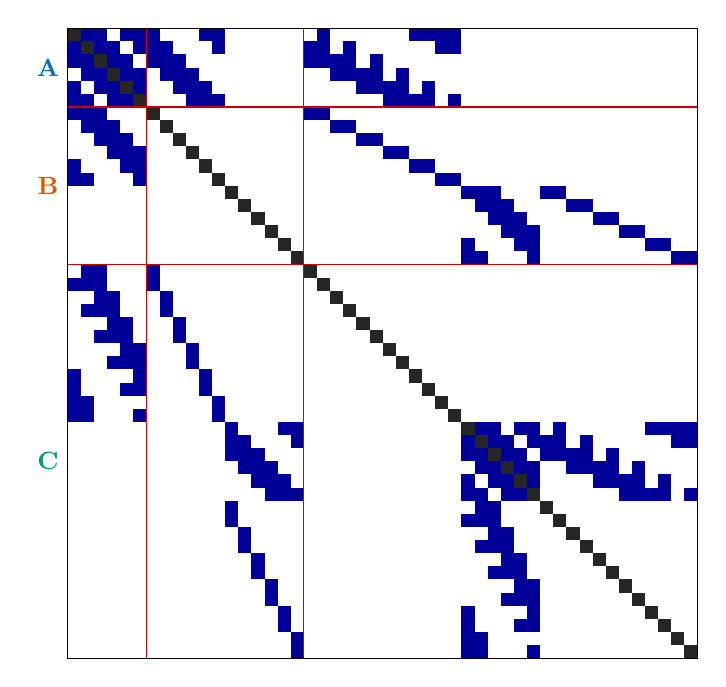
\begin{tikzpicture}[scale=1.0]
  \fill[black!85] (0.000,0.000) rectangle (0.167,-0.167);
  \fill[blue!60!black] (0.167,0.000) rectangle (0.333,-0.167);
  \fill[blue!60!black] (0.333,0.000) rectangle (0.500,-0.167);
  \fill[blue!60!black] (0.667,0.000) rectangle (0.833,-0.167);
  \fill[blue!60!black] (0.833,0.000) rectangle (1.000,-0.167);
  \fill[blue!60!black] (1.000,0.000) rectangle (1.167,-0.167);
  \fill[blue!60!black] (1.667,0.000) rectangle (1.833,-0.167);
  \fill[blue!60!black] (1.833,0.000) rectangle (2.000,-0.167);
  \fill[blue!60!black] (3.167,0.000) rectangle (3.333,-0.167);
  \fill[blue!60!black] (4.333,0.000) rectangle (4.500,-0.167);
  \fill[blue!60!black] (4.500,0.000) rectangle (4.667,-0.167);
  \fill[blue!60!black] (4.667,0.000) rectangle (4.833,-0.167);
  \fill[blue!60!black] (4.833,0.000) rectangle (5.000,-0.167);
  \fill[blue!60!black] (0.000,-0.167) rectangle (0.167,-0.333);
  \fill[black!85] (0.167,-0.167) rectangle (0.333,-0.333);
  \fill[blue!60!black] (0.333,-0.167) rectangle (0.500,-0.333);
  \fill[blue!60!black] (0.500,-0.167) rectangle (0.667,-0.333);
  \fill[blue!60!black] (0.833,-0.167) rectangle (1.000,-0.333);
  \fill[blue!60!black] (1.000,-0.167) rectangle (1.167,-0.333);
  \fill[blue!60!black] (1.167,-0.167) rectangle (1.333,-0.333);
  \fill[blue!60!black] (1.833,-0.167) rectangle (2.000,-0.333);
  \fill[blue!60!black] (3.000,-0.167) rectangle (3.167,-0.333);
  \fill[blue!60!black] (3.167,-0.167) rectangle (3.333,-0.333);
  \fill[blue!60!black] (3.500,-0.167) rectangle (3.667,-0.333);
  \fill[blue!60!black] (4.667,-0.167) rectangle (4.833,-0.333);
  \fill[blue!60!black] (4.833,-0.167) rectangle (5.000,-0.333);
  \fill[blue!60!black] (0.000,-0.333) rectangle (0.167,-0.500);
  \fill[blue!60!black] (0.167,-0.333) rectangle (0.333,-0.500);
  \fill[black!85] (0.333,-0.333) rectangle (0.500,-0.500);
  \fill[blue!60!black] (0.500,-0.333) rectangle (0.667,-0.500);
  \fill[blue!60!black] (0.667,-0.333) rectangle (0.833,-0.500);
  \fill[blue!60!black] (1.000,-0.333) rectangle (1.167,-0.500);
  \fill[blue!60!black] (1.167,-0.333) rectangle (1.333,-0.500);
  \fill[blue!60!black] (1.333,-0.333) rectangle (1.500,-0.500);
  \fill[blue!60!black] (3.000,-0.333) rectangle (3.167,-0.500);
  \fill[blue!60!black] (3.167,-0.333) rectangle (3.333,-0.500);
  \fill[blue!60!black] (3.333,-0.333) rectangle (3.500,-0.500);
  \fill[blue!60!black] (3.500,-0.333) rectangle (3.667,-0.500);
  \fill[blue!60!black] (3.833,-0.333) rectangle (4.000,-0.500);
  \fill[blue!60!black] (0.167,-0.500) rectangle (0.333,-0.667);
  \fill[blue!60!black] (0.333,-0.500) rectangle (0.500,-0.667);
  \fill[black!85] (0.500,-0.500) rectangle (0.667,-0.667);
  \fill[blue!60!black] (0.667,-0.500) rectangle (0.833,-0.667);
  \fill[blue!60!black] (0.833,-0.500) rectangle (1.000,-0.667);
  \fill[blue!60!black] (1.167,-0.500) rectangle (1.333,-0.667);
  \fill[blue!60!black] (1.333,-0.500) rectangle (1.500,-0.667);
  \fill[blue!60!black] (1.500,-0.500) rectangle (1.667,-0.667);
  \fill[blue!60!black] (3.333,-0.500) rectangle (3.500,-0.667);
  \fill[blue!60!black] (3.500,-0.500) rectangle (3.667,-0.667);
  \fill[blue!60!black] (3.667,-0.500) rectangle (3.833,-0.667);
  \fill[blue!60!black] (3.833,-0.500) rectangle (4.000,-0.667);
  \fill[blue!60!black] (4.167,-0.500) rectangle (4.333,-0.667);
  \fill[blue!60!black] (0.000,-0.667) rectangle (0.167,-0.833);
  \fill[blue!60!black] (0.333,-0.667) rectangle (0.500,-0.833);
  \fill[blue!60!black] (0.500,-0.667) rectangle (0.667,-0.833);
  \fill[black!85] (0.667,-0.667) rectangle (0.833,-0.833);
  \fill[blue!60!black] (0.833,-0.667) rectangle (1.000,-0.833);
  \fill[blue!60!black] (1.333,-0.667) rectangle (1.500,-0.833);
  \fill[blue!60!black] (1.500,-0.667) rectangle (1.667,-0.833);
  \fill[blue!60!black] (1.667,-0.667) rectangle (1.833,-0.833);
  \fill[blue!60!black] (3.667,-0.667) rectangle (3.833,-0.833);
  \fill[blue!60!black] (3.833,-0.667) rectangle (4.000,-0.833);
  \fill[blue!60!black] (4.000,-0.667) rectangle (4.167,-0.833);
  \fill[blue!60!black] (4.167,-0.667) rectangle (4.333,-0.833);
  \fill[blue!60!black] (4.500,-0.667) rectangle (4.667,-0.833);
  \fill[blue!60!black] (0.000,-0.833) rectangle (0.167,-1.000);
  \fill[blue!60!black] (0.167,-0.833) rectangle (0.333,-1.000);
  \fill[blue!60!black] (0.500,-0.833) rectangle (0.667,-1.000);
  \fill[blue!60!black] (0.667,-0.833) rectangle (0.833,-1.000);
  \fill[black!85] (0.833,-0.833) rectangle (1.000,-1.000);
  \fill[blue!60!black] (1.500,-0.833) rectangle (1.667,-1.000);
  \fill[blue!60!black] (1.667,-0.833) rectangle (1.833,-1.000);
  \fill[blue!60!black] (1.833,-0.833) rectangle (2.000,-1.000);
  \fill[blue!60!black] (4.000,-0.833) rectangle (4.167,-1.000);
  \fill[blue!60!black] (4.167,-0.833) rectangle (4.333,-1.000);
  \fill[blue!60!black] (4.333,-0.833) rectangle (4.500,-1.000);
  \fill[blue!60!black] (4.500,-0.833) rectangle (4.667,-1.000);
  \fill[blue!60!black] (4.833,-0.833) rectangle (5.000,-1.000);
  \fill[blue!60!black] (0.000,-1.000) rectangle (0.167,-1.167);
  \fill[blue!60!black] (0.167,-1.000) rectangle (0.333,-1.167);
  \fill[blue!60!black] (0.333,-1.000) rectangle (0.500,-1.167);
  \fill[black!85] (1.000,-1.000) rectangle (1.167,-1.167);
  \fill[blue!60!black] (3.000,-1.000) rectangle (3.167,-1.167);
  \fill[blue!60!black] (3.167,-1.000) rectangle (3.333,-1.167);
  \fill[blue!60!black] (0.167,-1.167) rectangle (0.333,-1.333);
  \fill[blue!60!black] (0.333,-1.167) rectangle (0.500,-1.333);
  \fill[blue!60!black] (0.500,-1.167) rectangle (0.667,-1.333);
  \fill[black!85] (1.167,-1.167) rectangle (1.333,-1.333);
  \fill[blue!60!black] (3.333,-1.167) rectangle (3.500,-1.333);
  \fill[blue!60!black] (3.500,-1.167) rectangle (3.667,-1.333);
  \fill[blue!60!black] (0.333,-1.333) rectangle (0.500,-1.500);
  \fill[blue!60!black] (0.500,-1.333) rectangle (0.667,-1.500);
  \fill[blue!60!black] (0.667,-1.333) rectangle (0.833,-1.500);
  \fill[black!85] (1.333,-1.333) rectangle (1.500,-1.500);
  \fill[blue!60!black] (3.667,-1.333) rectangle (3.833,-1.500);
  \fill[blue!60!black] (3.833,-1.333) rectangle (4.000,-1.500);
  \fill[blue!60!black] (0.500,-1.500) rectangle (0.667,-1.667);
  \fill[blue!60!black] (0.667,-1.500) rectangle (0.833,-1.667);
  \fill[blue!60!black] (0.833,-1.500) rectangle (1.000,-1.667);
  \fill[black!85] (1.500,-1.500) rectangle (1.667,-1.667);
  \fill[blue!60!black] (4.000,-1.500) rectangle (4.167,-1.667);
  \fill[blue!60!black] (4.167,-1.500) rectangle (4.333,-1.667);
  \fill[blue!60!black] (0.000,-1.667) rectangle (0.167,-1.833);
  \fill[blue!60!black] (0.667,-1.667) rectangle (0.833,-1.833);
  \fill[blue!60!black] (0.833,-1.667) rectangle (1.000,-1.833);
  \fill[black!85] (1.667,-1.667) rectangle (1.833,-1.833);
  \fill[blue!60!black] (4.333,-1.667) rectangle (4.500,-1.833);
  \fill[blue!60!black] (4.500,-1.667) rectangle (4.667,-1.833);
  \fill[blue!60!black] (0.000,-1.833) rectangle (0.167,-2.000);
  \fill[blue!60!black] (0.167,-1.833) rectangle (0.333,-2.000);
  \fill[blue!60!black] (0.833,-1.833) rectangle (1.000,-2.000);
  \fill[black!85] (1.833,-1.833) rectangle (2.000,-2.000);
  \fill[blue!60!black] (4.667,-1.833) rectangle (4.833,-2.000);
  \fill[blue!60!black] (4.833,-1.833) rectangle (5.000,-2.000);
  \fill[black!85] (2.000,-2.000) rectangle (2.167,-2.167);
  \fill[blue!60!black] (5.000,-2.000) rectangle (5.167,-2.167);
  \fill[blue!60!black] (5.167,-2.000) rectangle (5.333,-2.167);
  \fill[blue!60!black] (5.333,-2.000) rectangle (5.500,-2.167);
  \fill[blue!60!black] (6.000,-2.000) rectangle (6.167,-2.167);
  \fill[blue!60!black] (6.167,-2.000) rectangle (6.333,-2.167);
  \fill[black!85] (2.167,-2.167) rectangle (2.333,-2.333);
  \fill[blue!60!black] (5.167,-2.167) rectangle (5.333,-2.333);
  \fill[blue!60!black] (5.333,-2.167) rectangle (5.500,-2.333);
  \fill[blue!60!black] (5.500,-2.167) rectangle (5.667,-2.333);
  \fill[blue!60!black] (6.333,-2.167) rectangle (6.500,-2.333);
  \fill[blue!60!black] (6.500,-2.167) rectangle (6.667,-2.333);
  \fill[black!85] (2.333,-2.333) rectangle (2.500,-2.500);
  \fill[blue!60!black] (5.333,-2.333) rectangle (5.500,-2.500);
  \fill[blue!60!black] (5.500,-2.333) rectangle (5.667,-2.500);
  \fill[blue!60!black] (5.667,-2.333) rectangle (5.833,-2.500);
  \fill[blue!60!black] (6.667,-2.333) rectangle (6.833,-2.500);
  \fill[blue!60!black] (6.833,-2.333) rectangle (7.000,-2.500);
  \fill[black!85] (2.500,-2.500) rectangle (2.667,-2.667);
  \fill[blue!60!black] (5.500,-2.500) rectangle (5.667,-2.667);
  \fill[blue!60!black] (5.667,-2.500) rectangle (5.833,-2.667);
  \fill[blue!60!black] (5.833,-2.500) rectangle (6.000,-2.667);
  \fill[blue!60!black] (7.000,-2.500) rectangle (7.167,-2.667);
  \fill[blue!60!black] (7.167,-2.500) rectangle (7.333,-2.667);
  \fill[black!85] (2.667,-2.667) rectangle (2.833,-2.833);
  \fill[blue!60!black] (5.000,-2.667) rectangle (5.167,-2.833);
  \fill[blue!60!black] (5.667,-2.667) rectangle (5.833,-2.833);
  \fill[blue!60!black] (5.833,-2.667) rectangle (6.000,-2.833);
  \fill[blue!60!black] (7.333,-2.667) rectangle (7.500,-2.833);
  \fill[blue!60!black] (7.500,-2.667) rectangle (7.667,-2.833);
  \fill[black!85] (2.833,-2.833) rectangle (3.000,-3.000);
  \fill[blue!60!black] (5.000,-2.833) rectangle (5.167,-3.000);
  \fill[blue!60!black] (5.167,-2.833) rectangle (5.333,-3.000);
  \fill[blue!60!black] (5.833,-2.833) rectangle (6.000,-3.000);
  \fill[blue!60!black] (7.667,-2.833) rectangle (7.833,-3.000);
  \fill[blue!60!black] (7.833,-2.833) rectangle (8.000,-3.000);
  \fill[blue!60!black] (0.167,-3.000) rectangle (0.333,-3.167);
  \fill[blue!60!black] (0.333,-3.000) rectangle (0.500,-3.167);
  \fill[blue!60!black] (1.000,-3.000) rectangle (1.167,-3.167);
  \fill[black!85] (3.000,-3.000) rectangle (3.167,-3.167);
  \fill[blue!60!black] (0.000,-3.167) rectangle (0.167,-3.333);
  \fill[blue!60!black] (0.167,-3.167) rectangle (0.333,-3.333);
  \fill[blue!60!black] (0.333,-3.167) rectangle (0.500,-3.333);
  \fill[blue!60!black] (1.000,-3.167) rectangle (1.167,-3.333);
  \fill[black!85] (3.167,-3.167) rectangle (3.333,-3.333);
  \fill[blue!60!black] (0.333,-3.333) rectangle (0.500,-3.500);
  \fill[blue!60!black] (0.500,-3.333) rectangle (0.667,-3.500);
  \fill[blue!60!black] (1.167,-3.333) rectangle (1.333,-3.500);
  \fill[black!85] (3.333,-3.333) rectangle (3.500,-3.500);
  \fill[blue!60!black] (0.167,-3.500) rectangle (0.333,-3.667);
  \fill[blue!60!black] (0.333,-3.500) rectangle (0.500,-3.667);
  \fill[blue!60!black] (0.500,-3.500) rectangle (0.667,-3.667);
  \fill[blue!60!black] (1.167,-3.500) rectangle (1.333,-3.667);
  \fill[black!85] (3.500,-3.500) rectangle (3.667,-3.667);
  \fill[blue!60!black] (0.500,-3.667) rectangle (0.667,-3.833);
  \fill[blue!60!black] (0.667,-3.667) rectangle (0.833,-3.833);
  \fill[blue!60!black] (1.333,-3.667) rectangle (1.500,-3.833);
  \fill[black!85] (3.667,-3.667) rectangle (3.833,-3.833);
  \fill[blue!60!black] (0.333,-3.833) rectangle (0.500,-4.000);
  \fill[blue!60!black] (0.500,-3.833) rectangle (0.667,-4.000);
  \fill[blue!60!black] (0.667,-3.833) rectangle (0.833,-4.000);
  \fill[blue!60!black] (1.333,-3.833) rectangle (1.500,-4.000);
  \fill[black!85] (3.833,-3.833) rectangle (4.000,-4.000);
  \fill[blue!60!black] (0.667,-4.000) rectangle (0.833,-4.167);
  \fill[blue!60!black] (0.833,-4.000) rectangle (1.000,-4.167);
  \fill[blue!60!black] (1.500,-4.000) rectangle (1.667,-4.167);
  \fill[black!85] (4.000,-4.000) rectangle (4.167,-4.167);
  \fill[blue!60!black] (0.500,-4.167) rectangle (0.667,-4.333);
  \fill[blue!60!black] (0.667,-4.167) rectangle (0.833,-4.333);
  \fill[blue!60!black] (0.833,-4.167) rectangle (1.000,-4.333);
  \fill[blue!60!black] (1.500,-4.167) rectangle (1.667,-4.333);
  \fill[black!85] (4.167,-4.167) rectangle (4.333,-4.333);
  \fill[blue!60!black] (0.000,-4.333) rectangle (0.167,-4.500);
  \fill[blue!60!black] (0.833,-4.333) rectangle (1.000,-4.500);
  \fill[blue!60!black] (1.667,-4.333) rectangle (1.833,-4.500);
  \fill[black!85] (4.333,-4.333) rectangle (4.500,-4.500);
  \fill[blue!60!black] (0.000,-4.500) rectangle (0.167,-4.667);
  \fill[blue!60!black] (0.667,-4.500) rectangle (0.833,-4.667);
  \fill[blue!60!black] (0.833,-4.500) rectangle (1.000,-4.667);
  \fill[blue!60!black] (1.667,-4.500) rectangle (1.833,-4.667);
  \fill[black!85] (4.500,-4.500) rectangle (4.667,-4.667);
  \fill[blue!60!black] (0.000,-4.667) rectangle (0.167,-4.833);
  \fill[blue!60!black] (0.167,-4.667) rectangle (0.333,-4.833);
  \fill[blue!60!black] (1.833,-4.667) rectangle (2.000,-4.833);
  \fill[black!85] (4.667,-4.667) rectangle (4.833,-4.833);
  \fill[blue!60!black] (0.000,-4.833) rectangle (0.167,-5.000);
  \fill[blue!60!black] (0.167,-4.833) rectangle (0.333,-5.000);
  \fill[blue!60!black] (0.833,-4.833) rectangle (1.000,-5.000);
  \fill[blue!60!black] (1.833,-4.833) rectangle (2.000,-5.000);
  \fill[black!85] (4.833,-4.833) rectangle (5.000,-5.000);
  \fill[blue!60!black] (2.000,-5.000) rectangle (2.167,-5.167);
  \fill[blue!60!black] (2.667,-5.000) rectangle (2.833,-5.167);
  \fill[blue!60!black] (2.833,-5.000) rectangle (3.000,-5.167);
  \fill[black!85] (5.000,-5.000) rectangle (5.167,-5.167);
  \fill[blue!60!black] (5.167,-5.000) rectangle (5.333,-5.167);
  \fill[blue!60!black] (5.333,-5.000) rectangle (5.500,-5.167);
  \fill[blue!60!black] (5.667,-5.000) rectangle (5.833,-5.167);
  \fill[blue!60!black] (5.833,-5.000) rectangle (6.000,-5.167);
  \fill[blue!60!black] (6.167,-5.000) rectangle (6.333,-5.167);
  \fill[blue!60!black] (7.333,-5.000) rectangle (7.500,-5.167);
  \fill[blue!60!black] (7.500,-5.000) rectangle (7.667,-5.167);
  \fill[blue!60!black] (7.667,-5.000) rectangle (7.833,-5.167);
  \fill[blue!60!black] (7.833,-5.000) rectangle (8.000,-5.167);
  \fill[blue!60!black] (2.000,-5.167) rectangle (2.167,-5.333);
  \fill[blue!60!black] (2.167,-5.167) rectangle (2.333,-5.333);
  \fill[blue!60!black] (2.833,-5.167) rectangle (3.000,-5.333);
  \fill[blue!60!black] (5.000,-5.167) rectangle (5.167,-5.333);
  \fill[black!85] (5.167,-5.167) rectangle (5.333,-5.333);
  \fill[blue!60!black] (5.333,-5.167) rectangle (5.500,-5.333);
  \fill[blue!60!black] (5.500,-5.167) rectangle (5.667,-5.333);
  \fill[blue!60!black] (5.833,-5.167) rectangle (6.000,-5.333);
  \fill[blue!60!black] (6.000,-5.167) rectangle (6.167,-5.333);
  \fill[blue!60!black] (6.167,-5.167) rectangle (6.333,-5.333);
  \fill[blue!60!black] (6.500,-5.167) rectangle (6.667,-5.333);
  \fill[blue!60!black] (7.667,-5.167) rectangle (7.833,-5.333);
  \fill[blue!60!black] (7.833,-5.167) rectangle (8.000,-5.333);
  \fill[blue!60!black] (2.000,-5.333) rectangle (2.167,-5.500);
  \fill[blue!60!black] (2.167,-5.333) rectangle (2.333,-5.500);
  \fill[blue!60!black] (2.333,-5.333) rectangle (2.500,-5.500);
  \fill[blue!60!black] (5.000,-5.333) rectangle (5.167,-5.500);
  \fill[blue!60!black] (5.167,-5.333) rectangle (5.333,-5.500);
  \fill[black!85] (5.333,-5.333) rectangle (5.500,-5.500);
  \fill[blue!60!black] (5.500,-5.333) rectangle (5.667,-5.500);
  \fill[blue!60!black] (5.667,-5.333) rectangle (5.833,-5.500);
  \fill[blue!60!black] (6.000,-5.333) rectangle (6.167,-5.500);
  \fill[blue!60!black] (6.167,-5.333) rectangle (6.333,-5.500);
  \fill[blue!60!black] (6.333,-5.333) rectangle (6.500,-5.500);
  \fill[blue!60!black] (6.500,-5.333) rectangle (6.667,-5.500);
  \fill[blue!60!black] (6.833,-5.333) rectangle (7.000,-5.500);
  \fill[blue!60!black] (2.167,-5.500) rectangle (2.333,-5.667);
  \fill[blue!60!black] (2.333,-5.500) rectangle (2.500,-5.667);
  \fill[blue!60!black] (2.500,-5.500) rectangle (2.667,-5.667);
  \fill[blue!60!black] (5.167,-5.500) rectangle (5.333,-5.667);
  \fill[blue!60!black] (5.333,-5.500) rectangle (5.500,-5.667);
  \fill[black!85] (5.500,-5.500) rectangle (5.667,-5.667);
  \fill[blue!60!black] (5.667,-5.500) rectangle (5.833,-5.667);
  \fill[blue!60!black] (5.833,-5.500) rectangle (6.000,-5.667);
  \fill[blue!60!black] (6.333,-5.500) rectangle (6.500,-5.667);
  \fill[blue!60!black] (6.500,-5.500) rectangle (6.667,-5.667);
  \fill[blue!60!black] (6.667,-5.500) rectangle (6.833,-5.667);
  \fill[blue!60!black] (6.833,-5.500) rectangle (7.000,-5.667);
  \fill[blue!60!black] (7.167,-5.500) rectangle (7.333,-5.667);
  \fill[blue!60!black] (2.333,-5.667) rectangle (2.500,-5.833);
  \fill[blue!60!black] (2.500,-5.667) rectangle (2.667,-5.833);
  \fill[blue!60!black] (2.667,-5.667) rectangle (2.833,-5.833);
  \fill[blue!60!black] (5.000,-5.667) rectangle (5.167,-5.833);
  \fill[blue!60!black] (5.333,-5.667) rectangle (5.500,-5.833);
  \fill[blue!60!black] (5.500,-5.667) rectangle (5.667,-5.833);
  \fill[black!85] (5.667,-5.667) rectangle (5.833,-5.833);
  \fill[blue!60!black] (5.833,-5.667) rectangle (6.000,-5.833);
  \fill[blue!60!black] (6.667,-5.667) rectangle (6.833,-5.833);
  \fill[blue!60!black] (6.833,-5.667) rectangle (7.000,-5.833);
  \fill[blue!60!black] (7.000,-5.667) rectangle (7.167,-5.833);
  \fill[blue!60!black] (7.167,-5.667) rectangle (7.333,-5.833);
  \fill[blue!60!black] (7.500,-5.667) rectangle (7.667,-5.833);
  \fill[blue!60!black] (2.500,-5.833) rectangle (2.667,-6.000);
  \fill[blue!60!black] (2.667,-5.833) rectangle (2.833,-6.000);
  \fill[blue!60!black] (2.833,-5.833) rectangle (3.000,-6.000);
  \fill[blue!60!black] (5.000,-5.833) rectangle (5.167,-6.000);
  \fill[blue!60!black] (5.167,-5.833) rectangle (5.333,-6.000);
  \fill[blue!60!black] (5.500,-5.833) rectangle (5.667,-6.000);
  \fill[blue!60!black] (5.667,-5.833) rectangle (5.833,-6.000);
  \fill[black!85] (5.833,-5.833) rectangle (6.000,-6.000);
  \fill[blue!60!black] (7.000,-5.833) rectangle (7.167,-6.000);
  \fill[blue!60!black] (7.167,-5.833) rectangle (7.333,-6.000);
  \fill[blue!60!black] (7.333,-5.833) rectangle (7.500,-6.000);
  \fill[blue!60!black] (7.500,-5.833) rectangle (7.667,-6.000);
  \fill[blue!60!black] (7.833,-5.833) rectangle (8.000,-6.000);
  \fill[blue!60!black] (2.000,-6.000) rectangle (2.167,-6.167);
  \fill[blue!60!black] (5.167,-6.000) rectangle (5.333,-6.167);
  \fill[blue!60!black] (5.333,-6.000) rectangle (5.500,-6.167);
  \fill[black!85] (6.000,-6.000) rectangle (6.167,-6.167);
  \fill[blue!60!black] (2.000,-6.167) rectangle (2.167,-6.333);
  \fill[blue!60!black] (5.000,-6.167) rectangle (5.167,-6.333);
  \fill[blue!60!black] (5.167,-6.167) rectangle (5.333,-6.333);
  \fill[blue!60!black] (5.333,-6.167) rectangle (5.500,-6.333);
  \fill[black!85] (6.167,-6.167) rectangle (6.333,-6.333);
  \fill[blue!60!black] (2.167,-6.333) rectangle (2.333,-6.500);
  \fill[blue!60!black] (5.333,-6.333) rectangle (5.500,-6.500);
  \fill[blue!60!black] (5.500,-6.333) rectangle (5.667,-6.500);
  \fill[black!85] (6.333,-6.333) rectangle (6.500,-6.500);
  \fill[blue!60!black] (2.167,-6.500) rectangle (2.333,-6.667);
  \fill[blue!60!black] (5.167,-6.500) rectangle (5.333,-6.667);
  \fill[blue!60!black] (5.333,-6.500) rectangle (5.500,-6.667);
  \fill[blue!60!black] (5.500,-6.500) rectangle (5.667,-6.667);
  \fill[black!85] (6.500,-6.500) rectangle (6.667,-6.667);
  \fill[blue!60!black] (2.333,-6.667) rectangle (2.500,-6.833);
  \fill[blue!60!black] (5.500,-6.667) rectangle (5.667,-6.833);
  \fill[blue!60!black] (5.667,-6.667) rectangle (5.833,-6.833);
  \fill[black!85] (6.667,-6.667) rectangle (6.833,-6.833);
  \fill[blue!60!black] (2.333,-6.833) rectangle (2.500,-7.000);
  \fill[blue!60!black] (5.333,-6.833) rectangle (5.500,-7.000);
  \fill[blue!60!black] (5.500,-6.833) rectangle (5.667,-7.000);
  \fill[blue!60!black] (5.667,-6.833) rectangle (5.833,-7.000);
  \fill[black!85] (6.833,-6.833) rectangle (7.000,-7.000);
  \fill[blue!60!black] (2.500,-7.000) rectangle (2.667,-7.167);
  \fill[blue!60!black] (5.667,-7.000) rectangle (5.833,-7.167);
  \fill[blue!60!black] (5.833,-7.000) rectangle (6.000,-7.167);
  \fill[black!85] (7.000,-7.000) rectangle (7.167,-7.167);
  \fill[blue!60!black] (2.500,-7.167) rectangle (2.667,-7.333);
  \fill[blue!60!black] (5.500,-7.167) rectangle (5.667,-7.333);
  \fill[blue!60!black] (5.667,-7.167) rectangle (5.833,-7.333);
  \fill[blue!60!black] (5.833,-7.167) rectangle (6.000,-7.333);
  \fill[black!85] (7.167,-7.167) rectangle (7.333,-7.333);
  \fill[blue!60!black] (2.667,-7.333) rectangle (2.833,-7.500);
  \fill[blue!60!black] (5.000,-7.333) rectangle (5.167,-7.500);
  \fill[blue!60!black] (5.833,-7.333) rectangle (6.000,-7.500);
  \fill[black!85] (7.333,-7.333) rectangle (7.500,-7.500);
  \fill[blue!60!black] (2.667,-7.500) rectangle (2.833,-7.667);
  \fill[blue!60!black] (5.000,-7.500) rectangle (5.167,-7.667);
  \fill[blue!60!black] (5.667,-7.500) rectangle (5.833,-7.667);
  \fill[blue!60!black] (5.833,-7.500) rectangle (6.000,-7.667);
  \fill[black!85] (7.500,-7.500) rectangle (7.667,-7.667);
  \fill[blue!60!black] (2.833,-7.667) rectangle (3.000,-7.833);
  \fill[blue!60!black] (5.000,-7.667) rectangle (5.167,-7.833);
  \fill[blue!60!black] (5.167,-7.667) rectangle (5.333,-7.833);
  \fill[black!85] (7.667,-7.667) rectangle (7.833,-7.833);
  \fill[blue!60!black] (2.833,-7.833) rectangle (3.000,-8.000);
  \fill[blue!60!black] (5.000,-7.833) rectangle (5.167,-8.000);
  \fill[blue!60!black] (5.167,-7.833) rectangle (5.333,-8.000);
  \fill[blue!60!black] (5.833,-7.833) rectangle (6.000,-8.000);
  \fill[black!85] (7.833,-7.833) rectangle (8.000,-8.000);
  \draw[red!80!black, line width=0.4pt] (1.000,0.000) -- (1.000,-8.000);
  \draw[red!80!black, line width=0.4pt] (0,-1.000) -- (8.000,-1.000);
  \draw[red!80!black, line width=0.4pt] (3.000,0.000) -- (3.000,-8.000);
  \draw[red!80!black, line width=0.4pt] (0,-3.000) -- (8.000,-3.000);
  \draw[black, line width=0.3pt] (0,0) rectangle (8.000,-8.000);
  \definecolor{hml0}{rgb}{0.000, 0.450, 0.700}
  \node[font=\small\bfseries, hml0] at (-0.25,-0.500) {A};
  \definecolor{hml1}{rgb}{0.840, 0.370, 0.000}
  \node[font=\small\bfseries, hml1] at (-0.25,-2.000) {B};
  \definecolor{hml2}{rgb}{0.000, 0.620, 0.450}
  \node[font=\small\bfseries, hml2] at (-0.25,-5.500) {C};
\end{tikzpicture}
  \caption{Adjacency heatmap (rows/columns sorted by tier): the binary co-occurrence shadow of the ternary structure above; included as a tier-block-structure diagnostic.}
\end{subfigure}
\caption{$Q_{48} = Q_{24} \cup \Ccls(Q_{24})$: three views of the $\Ccls$-closure of the canonical 6-vertex Rosen-closed seed graph. Tier counts $|A|/|B|/|C| = 6/12/30$.}
\label{fig:q48}
\end{figure}
% Auto-generated by paper/scripts/dump_quotient_to_tikz.py
% Do not hand-edit; regenerate via `python3 dump_quotient_to_tikz.py`.
\begin{figure}[H]
\centering
\begin{subfigure}[t]{\textwidth}
  \centering
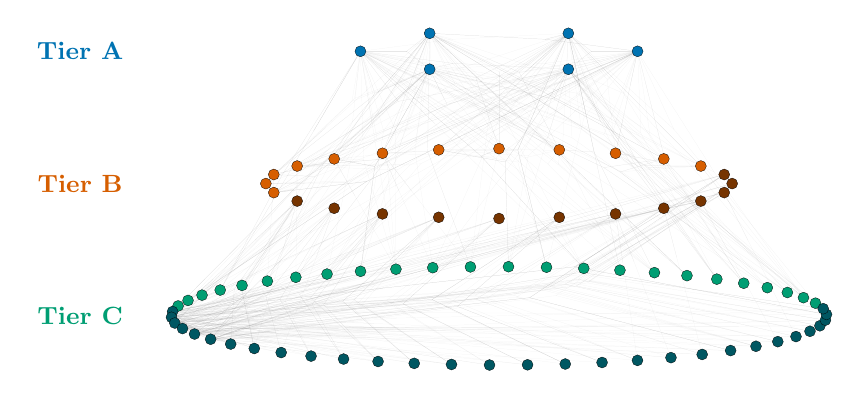
\begin{tikzpicture}[scale=1.4]
  \draw[gray, line width=0.08pt, opacity=0.10] (1.257,1.200) -- (0.419,1.309);
  \draw[gray, line width=0.08pt, opacity=0.10] (0.629,1.363) -- (0.419,1.309);
  \draw[gray, line width=0.08pt, opacity=0.10] (-0.629,1.363) -- (0.419,1.309);
  \draw[gray, line width=0.08pt, opacity=0.10] (1.257,1.200) -- (0.419,1.091);
  \draw[gray, line width=0.08pt, opacity=0.10] (-0.629,1.037) -- (0.419,1.091);
  \draw[gray, line width=0.08pt, opacity=0.10] (0.629,1.037) -- (0.419,1.091);
  \draw[gray, line width=0.08pt, opacity=0.10] (1.257,1.200) -- (1.191,0.892);
  \draw[gray, line width=0.08pt, opacity=0.10] (1.057,0.275) -- (1.191,0.892);
  \draw[gray, line width=0.08pt, opacity=0.10] (1.257,1.200) -- (1.191,0.892);
  \draw[gray, line width=0.08pt, opacity=0.10] (1.257,1.200) -- (1.512,0.190);
  \draw[gray, line width=0.08pt, opacity=0.10] (1.057,0.275) -- (1.512,0.190);
  \draw[gray, line width=0.08pt, opacity=0.10] (2.220,-0.904) -- (1.512,0.190);
  \draw[gray, line width=0.08pt, opacity=0.10] (1.257,1.200) -- (-0.143,0.946);
  \draw[gray, line width=0.08pt, opacity=0.10] (-1.057,0.275) -- (-0.143,0.946);
  \draw[gray, line width=0.08pt, opacity=0.10] (-0.629,1.363) -- (-0.143,0.946);
  \draw[gray, line width=0.08pt, opacity=0.10] (1.257,1.200) -- (-0.401,0.907);
  \draw[gray, line width=0.08pt, opacity=0.10] (-1.831,0.159) -- (-0.401,0.907);
  \draw[gray, line width=0.08pt, opacity=0.10] (-0.629,1.363) -- (-0.401,0.907);
  \draw[gray, line width=0.08pt, opacity=0.10] (1.257,1.200) -- (0.157,0.773);
  \draw[gray, line width=0.08pt, opacity=0.10] (-2.043,-0.082) -- (0.157,0.773);
  \draw[gray, line width=0.08pt, opacity=0.10] (1.257,1.200) -- (0.157,0.773);
  \draw[gray, line width=0.08pt, opacity=0.10] (1.257,1.200) -- (-1.202,0.019);
  \draw[gray, line width=0.08pt, opacity=0.10] (-2.043,-0.082) -- (-1.202,0.019);
  \draw[gray, line width=0.08pt, opacity=0.10] (-2.821,-1.060) -- (-1.202,0.019);
  \draw[gray, line width=0.08pt, opacity=0.10] (1.257,1.200) -- (1.369,0.444);
  \draw[gray, line width=0.08pt, opacity=0.10] (2.220,-0.904) -- (1.369,0.444);
  \draw[gray, line width=0.08pt, opacity=0.10] (0.629,1.037) -- (1.369,0.444);
  \draw[gray, line width=0.08pt, opacity=0.10] (1.257,1.200) -- (0.428,0.600);
  \draw[gray, line width=0.08pt, opacity=0.10] (-0.601,-0.763) -- (0.428,0.600);
  \draw[gray, line width=0.08pt, opacity=0.10] (0.629,1.363) -- (0.428,0.600);
  \draw[gray, line width=0.08pt, opacity=0.10] (1.257,1.200) -- (0.014,0.571);
  \draw[gray, line width=0.08pt, opacity=0.10] (-1.843,-0.850) -- (0.014,0.571);
  \draw[gray, line width=0.08pt, opacity=0.10] (0.629,1.363) -- (0.014,0.571);
  \draw[gray, line width=0.08pt, opacity=0.10] (1.257,1.200) -- (-0.806,0.169);
  \draw[gray, line width=0.08pt, opacity=0.10] (-1.843,-0.850) -- (-0.806,0.169);
  \draw[gray, line width=0.08pt, opacity=0.10] (-1.831,0.159) -- (-0.806,0.169);
  \draw[gray, line width=0.08pt, opacity=0.10] (1.257,1.200) -- (-1.202,0.019);
  \draw[gray, line width=0.08pt, opacity=0.10] (-2.821,-1.060) -- (-1.202,0.019);
  \draw[gray, line width=0.08pt, opacity=0.10] (-2.043,-0.082) -- (-1.202,0.019);
  \draw[gray, line width=0.08pt, opacity=0.10] (0.629,1.363) -- (0.419,1.309);
  \draw[gray, line width=0.08pt, opacity=0.10] (-0.629,1.363) -- (0.419,1.309);
  \draw[gray, line width=0.08pt, opacity=0.10] (1.257,1.200) -- (0.419,1.309);
  \draw[gray, line width=0.08pt, opacity=0.10] (0.629,1.363) -- (0.838,1.200);
  \draw[gray, line width=0.08pt, opacity=0.10] (0.629,1.037) -- (0.838,1.200);
  \draw[gray, line width=0.08pt, opacity=0.10] (1.257,1.200) -- (0.838,1.200);
  \draw[gray, line width=0.08pt, opacity=0.10] (0.629,1.363) -- (0.401,0.907);
  \draw[gray, line width=0.08pt, opacity=0.10] (1.831,0.159) -- (0.401,0.907);
  \draw[gray, line width=0.08pt, opacity=0.10] (-1.257,1.200) -- (0.401,0.907);
  \draw[gray, line width=0.08pt, opacity=0.10] (0.629,1.363) -- (0.000,1.015);
  \draw[gray, line width=0.08pt, opacity=0.10] (0.000,0.317) -- (0.000,1.015);
  \draw[gray, line width=0.08pt, opacity=0.10] (-0.629,1.363) -- (0.000,1.015);
  \draw[gray, line width=0.08pt, opacity=0.10] (0.629,1.363) -- (0.237,1.011);
  \draw[gray, line width=0.08pt, opacity=0.10] (-0.547,0.306) -- (0.237,1.011);
  \draw[gray, line width=0.08pt, opacity=0.10] (0.629,1.363) -- (0.237,1.011);
  \draw[gray, line width=0.08pt, opacity=0.10] (0.629,1.363) -- (0.018,0.907);
  \draw[gray, line width=0.08pt, opacity=0.10] (-1.831,0.159) -- (0.018,0.907);
  \draw[gray, line width=0.08pt, opacity=0.10] (1.257,1.200) -- (0.018,0.907);
  \draw[gray, line width=0.08pt, opacity=0.10] (0.629,1.363) -- (-0.191,0.853);
  \draw[gray, line width=0.08pt, opacity=0.10] (-1.831,0.159) -- (-0.191,0.853);
  \draw[gray, line width=0.08pt, opacity=0.10] (0.629,1.037) -- (-0.191,0.853);
  \draw[gray, line width=0.08pt, opacity=0.10] (0.629,1.363) -- (0.957,0.547);
  \draw[gray, line width=0.08pt, opacity=0.10] (2.871,-1.085) -- (0.957,0.547);
  \draw[gray, line width=0.08pt, opacity=0.10] (-0.629,1.363) -- (0.957,0.547);
  \draw[gray, line width=0.08pt, opacity=0.10] (0.629,1.363) -- (0.785,0.647);
  \draw[gray, line width=0.08pt, opacity=0.10] (1.097,-0.786) -- (0.785,0.647);
  \draw[gray, line width=0.08pt, opacity=0.10] (0.629,1.363) -- (0.785,0.647);
  \draw[gray, line width=0.08pt, opacity=0.10] (0.629,1.363) -- (0.772,0.601);
  \draw[gray, line width=0.08pt, opacity=0.10] (0.431,-0.759) -- (0.772,0.601);
  \draw[gray, line width=0.08pt, opacity=0.10] (1.257,1.200) -- (0.772,0.601);
  \draw[gray, line width=0.08pt, opacity=0.10] (0.629,1.363) -- (0.171,0.304);
  \draw[gray, line width=0.08pt, opacity=0.10] (0.431,-0.759) -- (0.171,0.304);
  \draw[gray, line width=0.08pt, opacity=0.10] (-0.547,0.306) -- (0.171,0.304);
  \draw[gray, line width=0.08pt, opacity=0.10] (0.629,1.363) -- (-0.101,0.526);
  \draw[gray, line width=0.08pt, opacity=0.10] (-1.560,-0.821) -- (-0.101,0.526);
  \draw[gray, line width=0.08pt, opacity=0.10] (0.629,1.037) -- (-0.101,0.526);
  \draw[gray, line width=0.08pt, opacity=0.10] (-0.629,1.363) -- (0.419,1.309);
  \draw[gray, line width=0.08pt, opacity=0.10] (0.629,1.363) -- (0.419,1.309);
  \draw[gray, line width=0.08pt, opacity=0.10] (1.257,1.200) -- (0.419,1.309);
  \draw[gray, line width=0.08pt, opacity=0.10] (-0.629,1.363) -- (-0.838,1.200);
  \draw[gray, line width=0.08pt, opacity=0.10] (-1.257,1.200) -- (-0.838,1.200);
  \draw[gray, line width=0.08pt, opacity=0.10] (-0.629,1.037) -- (-0.838,1.200);
  \draw[gray, line width=0.08pt, opacity=0.10] (-0.629,1.363) -- (0.191,0.962);
  \draw[gray, line width=0.08pt, opacity=0.10] (1.831,0.159) -- (0.191,0.962);
  \draw[gray, line width=0.08pt, opacity=0.10] (-0.629,1.363) -- (0.191,0.962);
  \draw[gray, line width=0.08pt, opacity=0.10] (-0.629,1.363) -- (0.182,1.011);
  \draw[gray, line width=0.08pt, opacity=0.10] (0.547,0.306) -- (0.182,1.011);
  \draw[gray, line width=0.08pt, opacity=0.10] (0.629,1.363) -- (0.182,1.011);
  \draw[gray, line width=0.08pt, opacity=0.10] (-0.629,1.363) -- (0.541,0.278);
  \draw[gray, line width=0.08pt, opacity=0.10] (0.547,0.306) -- (0.541,0.278);
  \draw[gray, line width=0.08pt, opacity=0.10] (1.705,-0.835) -- (0.541,0.278);
  \draw[gray, line width=0.08pt, opacity=0.10] (-0.629,1.363) -- (-0.772,1.000);
  \draw[gray, line width=0.08pt, opacity=0.10] (-1.057,0.275) -- (-0.772,1.000);
  \draw[gray, line width=0.08pt, opacity=0.10] (-0.629,1.363) -- (-0.772,1.000);
  \draw[gray, line width=0.08pt, opacity=0.10] (-0.629,1.363) -- (-1.100,0.827);
  \draw[gray, line width=0.08pt, opacity=0.10] (-2.043,0.082) -- (-1.100,0.827);
  \draw[gray, line width=0.08pt, opacity=0.10] (-0.629,1.037) -- (-1.100,0.827);
  \draw[gray, line width=0.08pt, opacity=0.10] (-0.629,1.363) -- (0.921,0.564);
  \draw[gray, line width=0.08pt, opacity=0.10] (2.762,-1.035) -- (0.921,0.564);
  \draw[gray, line width=0.08pt, opacity=0.10] (0.629,1.363) -- (0.921,0.564);
  \draw[gray, line width=0.08pt, opacity=0.10] (-0.629,1.363) -- (1.322,0.162);
  \draw[gray, line width=0.08pt, opacity=0.10] (2.762,-1.035) -- (1.322,0.162);
  \draw[gray, line width=0.08pt, opacity=0.10] (1.831,0.159) -- (1.322,0.162);
  \draw[gray, line width=0.08pt, opacity=0.10] (-0.629,1.363) -- (0.149,0.522);
  \draw[gray, line width=0.08pt, opacity=0.10] (1.705,-0.835) -- (0.149,0.522);
  \draw[gray, line width=0.08pt, opacity=0.10] (-0.629,1.037) -- (0.149,0.522);
  \draw[gray, line width=0.08pt, opacity=0.10] (-0.629,1.363) -- (-0.086,0.657);
  \draw[gray, line width=0.08pt, opacity=0.10] (-0.259,-0.756) -- (-0.086,0.657);
  \draw[gray, line width=0.08pt, opacity=0.10] (0.629,1.363) -- (-0.086,0.657);
  \draw[gray, line width=0.08pt, opacity=0.10] (-0.629,1.363) -- (-1.329,0.560);
  \draw[gray, line width=0.08pt, opacity=0.10] (-2.101,-0.885) -- (-1.329,0.560);
  \draw[gray, line width=0.08pt, opacity=0.10] (-1.257,1.200) -- (-1.329,0.560);
  \draw[gray, line width=0.08pt, opacity=0.10] (-1.257,1.200) -- (-0.419,1.309);
  \draw[gray, line width=0.08pt, opacity=0.10] (0.629,1.363) -- (-0.419,1.309);
  \draw[gray, line width=0.08pt, opacity=0.10] (-0.629,1.363) -- (-0.419,1.309);
  \draw[gray, line width=0.08pt, opacity=0.10] (-1.257,1.200) -- (-0.838,1.200);
  \draw[gray, line width=0.08pt, opacity=0.10] (-0.629,1.037) -- (-0.838,1.200);
  \draw[gray, line width=0.08pt, opacity=0.10] (-0.629,1.363) -- (-0.838,1.200);
  \draw[gray, line width=0.08pt, opacity=0.10] (-1.257,1.200) -- (-0.446,0.957);
  \draw[gray, line width=0.08pt, opacity=0.10] (0.547,0.306) -- (-0.446,0.957);
  \draw[gray, line width=0.08pt, opacity=0.10] (-0.629,1.363) -- (-0.446,0.957);
  \draw[gray, line width=0.08pt, opacity=0.10] (-1.257,1.200) -- (0.233,0.233);
  \draw[gray, line width=0.08pt, opacity=0.10] (0.547,0.306) -- (0.233,0.233);
  \draw[gray, line width=0.08pt, opacity=0.10] (1.410,-0.808) -- (0.233,0.233);
  \draw[gray, line width=0.08pt, opacity=0.10] (-1.257,1.200) -- (-0.163,0.249);
  \draw[gray, line width=0.08pt, opacity=0.10] (0.000,0.317) -- (-0.163,0.249);
  \draw[gray, line width=0.08pt, opacity=0.10] (0.769,-0.769) -- (-0.163,0.249);
  \draw[gray, line width=0.08pt, opacity=0.10] (-1.257,1.200) -- (-1.127,0.820);
  \draw[gray, line width=0.08pt, opacity=0.10] (-1.495,0.224) -- (-1.127,0.820);
  \draw[gray, line width=0.08pt, opacity=0.10] (-0.629,1.037) -- (-1.127,0.820);
  \draw[gray, line width=0.08pt, opacity=0.10] (-1.257,1.200) -- (-1.334,0.746);
  \draw[gray, line width=0.08pt, opacity=0.10] (-2.115,0.000) -- (-1.334,0.746);
  \draw[gray, line width=0.08pt, opacity=0.10] (-0.629,1.037) -- (-1.334,0.746);
  \draw[gray, line width=0.08pt, opacity=0.10] (-1.257,1.200) -- (0.261,0.585);
  \draw[gray, line width=0.08pt, opacity=0.10] (1.410,-0.808) -- (0.261,0.585);
  \draw[gray, line width=0.08pt, opacity=0.10] (0.629,1.363) -- (0.261,0.585);
  \draw[gray, line width=0.08pt, opacity=0.10] (-1.257,1.200) -- (-0.158,0.476);
  \draw[gray, line width=0.08pt, opacity=0.10] (1.410,-0.808) -- (-0.158,0.476);
  \draw[gray, line width=0.08pt, opacity=0.10] (-0.629,1.037) -- (-0.158,0.476);
  \draw[gray, line width=0.08pt, opacity=0.10] (-1.257,1.200) -- (-0.582,0.544);
  \draw[gray, line width=0.08pt, opacity=0.10] (0.769,-0.769) -- (-0.582,0.544);
  \draw[gray, line width=0.08pt, opacity=0.10] (-1.257,1.200) -- (-0.582,0.544);
  \draw[gray, line width=0.08pt, opacity=0.10] (-1.257,1.200) -- (-1.150,0.541);
  \draw[gray, line width=0.08pt, opacity=0.10] (-0.935,-0.777) -- (-1.150,0.541);
  \draw[gray, line width=0.08pt, opacity=0.10] (-1.257,1.200) -- (-1.150,0.541);
  \draw[gray, line width=0.08pt, opacity=0.10] (-1.257,1.200) -- (-1.681,0.478);
  \draw[gray, line width=0.08pt, opacity=0.10] (-2.529,-0.966) -- (-1.681,0.478);
  \draw[gray, line width=0.08pt, opacity=0.10] (-1.257,1.200) -- (-1.681,0.478);
  \draw[gray, line width=0.08pt, opacity=0.10] (-1.257,1.200) -- (-1.967,0.078);
  \draw[gray, line width=0.08pt, opacity=0.10] (-2.529,-0.966) -- (-1.967,0.078);
  \draw[gray, line width=0.08pt, opacity=0.10] (-2.115,0.000) -- (-1.967,0.078);
  \draw[gray, line width=0.08pt, opacity=0.10] (-0.629,1.037) -- (-0.419,1.091);
  \draw[gray, line width=0.08pt, opacity=0.10] (-1.257,1.200) -- (-0.419,1.091);
  \draw[gray, line width=0.08pt, opacity=0.10] (0.629,1.037) -- (-0.419,1.091);
  \draw[gray, line width=0.08pt, opacity=0.10] (-0.629,1.037) -- (0.708,0.820);
  \draw[gray, line width=0.08pt, opacity=0.10] (1.495,0.224) -- (0.708,0.820);
  \draw[gray, line width=0.08pt, opacity=0.10] (1.257,1.200) -- (0.708,0.820);
  \draw[gray, line width=0.08pt, opacity=0.10] (-0.629,1.037) -- (0.498,0.766);
  \draw[gray, line width=0.08pt, opacity=0.10] (1.495,0.224) -- (0.498,0.766);
  \draw[gray, line width=0.08pt, opacity=0.10] (0.629,1.037) -- (0.498,0.766);
  \draw[gray, line width=0.08pt, opacity=0.10] (-0.629,1.037) -- (-0.918,0.766);
  \draw[gray, line width=0.08pt, opacity=0.10] (-1.495,0.224) -- (-0.918,0.766);
  \draw[gray, line width=0.08pt, opacity=0.10] (-0.629,1.037) -- (-0.918,0.766);
  \draw[gray, line width=0.08pt, opacity=0.10] (-0.629,1.037) -- (-1.100,0.827);
  \draw[gray, line width=0.08pt, opacity=0.10] (-2.043,0.082) -- (-1.100,0.827);
  \draw[gray, line width=0.08pt, opacity=0.10] (-0.629,1.363) -- (-1.100,0.827);
  \draw[gray, line width=0.08pt, opacity=0.10] (-0.629,1.037) -- (-0.471,0.718);
  \draw[gray, line width=0.08pt, opacity=0.10] (-2.043,-0.082) -- (-0.471,0.718);
  \draw[gray, line width=0.08pt, opacity=0.10] (1.257,1.200) -- (-0.471,0.718);
  \draw[gray, line width=0.08pt, opacity=0.10] (-0.629,1.037) -- (-1.861,-0.052);
  \draw[gray, line width=0.08pt, opacity=0.10] (-2.043,-0.082) -- (-1.861,-0.052);
  \draw[gray, line width=0.08pt, opacity=0.10] (-2.911,-1.110) -- (-1.861,-0.052);
  \draw[gray, line width=0.08pt, opacity=0.10] (-0.629,1.037) -- (0.392,0.376);
  \draw[gray, line width=0.08pt, opacity=0.10] (2.434,-0.944) -- (0.392,0.376);
  \draw[gray, line width=0.08pt, opacity=0.10] (-0.629,1.037) -- (0.392,0.376);
  \draw[gray, line width=0.08pt, opacity=0.10] (-0.629,1.037) -- (-1.047,0.480);
  \draw[gray, line width=0.08pt, opacity=0.10] (-1.256,-0.796) -- (-1.047,0.480);
  \draw[gray, line width=0.08pt, opacity=0.10] (-1.257,1.200) -- (-1.047,0.480);
  \draw[gray, line width=0.08pt, opacity=0.10] (-0.629,1.037) -- (-1.127,0.155);
  \draw[gray, line width=0.08pt, opacity=0.10] (-1.256,-0.796) -- (-1.127,0.155);
  \draw[gray, line width=0.08pt, opacity=0.10] (-1.495,0.224) -- (-1.127,0.155);
  \draw[gray, line width=0.08pt, opacity=0.10] (-0.629,1.037) -- (-1.668,0.065);
  \draw[gray, line width=0.08pt, opacity=0.10] (-2.331,-0.924) -- (-1.668,0.065);
  \draw[gray, line width=0.08pt, opacity=0.10] (-2.043,0.082) -- (-1.668,0.065);
  \draw[gray, line width=0.08pt, opacity=0.10] (-0.629,1.037) -- (-0.970,0.321);
  \draw[gray, line width=0.08pt, opacity=0.10] (-2.911,-1.110) -- (-0.970,0.321);
  \draw[gray, line width=0.08pt, opacity=0.10] (0.629,1.037) -- (-0.970,0.321);
  \draw[gray, line width=0.08pt, opacity=0.10] (0.629,1.037) -- (0.838,1.200);
  \draw[gray, line width=0.08pt, opacity=0.10] (0.629,1.363) -- (0.838,1.200);
  \draw[gray, line width=0.08pt, opacity=0.10] (1.257,1.200) -- (0.838,1.200);
  \draw[gray, line width=0.08pt, opacity=0.10] (0.629,1.037) -- (-0.419,1.091);
  \draw[gray, line width=0.08pt, opacity=0.10] (-0.629,1.037) -- (-0.419,1.091);
  \draw[gray, line width=0.08pt, opacity=0.10] (-1.257,1.200) -- (-0.419,1.091);
  \draw[gray, line width=0.08pt, opacity=0.10] (0.629,1.037) -- (0.498,0.766);
  \draw[gray, line width=0.08pt, opacity=0.10] (1.495,0.224) -- (0.498,0.766);
  \draw[gray, line width=0.08pt, opacity=0.10] (-0.629,1.037) -- (0.498,0.766);
  \draw[gray, line width=0.08pt, opacity=0.10] (0.629,1.037) -- (0.772,0.892);
  \draw[gray, line width=0.08pt, opacity=0.10] (1.057,0.275) -- (0.772,0.892);
  \draw[gray, line width=0.08pt, opacity=0.10] (0.629,1.363) -- (0.772,0.892);
  \draw[gray, line width=0.08pt, opacity=0.10] (0.629,1.037) -- (1.221,0.148);
  \draw[gray, line width=0.08pt, opacity=0.10] (1.057,0.275) -- (1.221,0.148);
  \draw[gray, line width=0.08pt, opacity=0.10] (1.976,-0.867) -- (1.221,0.148);
  \draw[gray, line width=0.08pt, opacity=0.10] (0.629,1.037) -- (0.056,0.196);
  \draw[gray, line width=0.08pt, opacity=0.10] (-0.547,0.306) -- (0.056,0.196);
  \draw[gray, line width=0.08pt, opacity=0.10] (0.086,-0.754) -- (0.056,0.196);
  \draw[gray, line width=0.08pt, opacity=0.10] (0.629,1.037) -- (-0.286,0.691);
  \draw[gray, line width=0.08pt, opacity=0.10] (-2.115,0.000) -- (-0.286,0.691);
  \draw[gray, line width=0.08pt, opacity=0.10] (0.629,1.037) -- (-0.286,0.691);
  \draw[gray, line width=0.08pt, opacity=0.10] (0.629,1.037) -- (0.662,0.416);
  \draw[gray, line width=0.08pt, opacity=0.10] (2.616,-0.988) -- (0.662,0.416);
  \draw[gray, line width=0.08pt, opacity=0.10] (-1.257,1.200) -- (0.662,0.416);
  \draw[gray, line width=0.08pt, opacity=0.10] (0.629,1.037) -- (1.287,0.457);
  \draw[gray, line width=0.08pt, opacity=0.10] (1.976,-0.867) -- (1.287,0.457);
  \draw[gray, line width=0.08pt, opacity=0.10] (1.257,1.200) -- (1.287,0.457);
  \draw[gray, line width=0.08pt, opacity=0.10] (0.629,1.037) -- (1.078,0.402);
  \draw[gray, line width=0.08pt, opacity=0.10] (1.976,-0.867) -- (1.078,0.402);
  \draw[gray, line width=0.08pt, opacity=0.10] (0.629,1.037) -- (1.078,0.402);
  \draw[gray, line width=0.08pt, opacity=0.10] (0.629,1.037) -- (0.448,0.440);
  \draw[gray, line width=0.08pt, opacity=0.10] (0.086,-0.754) -- (0.448,0.440);
  \draw[gray, line width=0.08pt, opacity=0.10] (0.629,1.037) -- (0.448,0.440);
  \draw[gray, line width=0.08pt, opacity=0.10] (0.629,1.037) -- (-0.898,0.354);
  \draw[gray, line width=0.08pt, opacity=0.10] (-2.694,-1.012) -- (-0.898,0.354);
  \draw[gray, line width=0.08pt, opacity=0.10] (-0.629,1.037) -- (-0.898,0.354);
  \draw[gray, line width=0.08pt, opacity=0.10] (1.831,0.159) -- (1.030,0.962);
  \draw[gray, line width=0.08pt, opacity=0.10] (0.629,1.363) -- (1.030,0.962);
  \draw[gray, line width=0.08pt, opacity=0.10] (0.629,1.363) -- (1.030,0.962);
  \draw[gray, line width=0.08pt, opacity=0.10] (1.831,0.159) -- (1.430,0.560);
  \draw[gray, line width=0.08pt, opacity=0.10] (0.629,1.363) -- (1.430,0.560);
  \draw[gray, line width=0.08pt, opacity=0.10] (1.831,0.159) -- (1.430,0.560);
  \draw[gray, line width=0.08pt, opacity=0.10] (1.831,0.159) -- (0.610,0.962);
  \draw[gray, line width=0.08pt, opacity=0.10] (-0.629,1.363) -- (0.610,0.962);
  \draw[gray, line width=0.08pt, opacity=0.10] (0.629,1.363) -- (0.610,0.962);
  \draw[gray, line width=0.08pt, opacity=0.10] (1.831,0.159) -- (1.322,0.162);
  \draw[gray, line width=0.08pt, opacity=0.10] (-0.629,1.363) -- (1.322,0.162);
  \draw[gray, line width=0.08pt, opacity=0.10] (2.762,-1.035) -- (1.322,0.162);
  \draw[gray, line width=0.08pt, opacity=0.10] (1.831,0.159) -- (1.358,0.146);
  \draw[gray, line width=0.08pt, opacity=0.10] (2.871,-1.085) -- (1.358,0.146);
  \draw[gray, line width=0.08pt, opacity=0.10] (-0.629,1.363) -- (1.358,0.146);
  \draw[gray, line width=0.08pt, opacity=0.10] (1.831,0.159) -- (1.741,0.162);
  \draw[gray, line width=0.08pt, opacity=0.10] (2.762,-1.035) -- (1.741,0.162);
  \draw[gray, line width=0.08pt, opacity=0.10] (0.629,1.363) -- (1.741,0.162);
  \draw[gray, line width=0.08pt, opacity=0.10] (1.831,0.159) -- (2.142,-0.239);
  \draw[gray, line width=0.08pt, opacity=0.10] (2.762,-1.035) -- (2.142,-0.239);
  \draw[gray, line width=0.08pt, opacity=0.10] (1.831,0.159) -- (2.142,-0.239);
  \draw[gray, line width=0.08pt, opacity=0.10] (1.495,0.224) -- (0.498,0.766);
  \draw[gray, line width=0.08pt, opacity=0.10] (-0.629,1.037) -- (0.498,0.766);
  \draw[gray, line width=0.08pt, opacity=0.10] (0.629,1.037) -- (0.498,0.766);
  \draw[gray, line width=0.08pt, opacity=0.10] (1.495,0.224) -- (1.127,0.820);
  \draw[gray, line width=0.08pt, opacity=0.10] (0.629,1.037) -- (1.127,0.820);
  \draw[gray, line width=0.08pt, opacity=0.10] (1.257,1.200) -- (1.127,0.820);
  \draw[gray, line width=0.08pt, opacity=0.10] (1.495,0.224) -- (0.918,0.766);
  \draw[gray, line width=0.08pt, opacity=0.10] (0.629,1.037) -- (0.918,0.766);
  \draw[gray, line width=0.08pt, opacity=0.10] (0.629,1.037) -- (0.918,0.766);
  \draw[gray, line width=0.08pt, opacity=0.10] (1.495,0.224) -- (0.951,0.145);
  \draw[gray, line width=0.08pt, opacity=0.10] (2.616,-0.988) -- (0.951,0.145);
  \draw[gray, line width=0.08pt, opacity=0.10] (-1.257,1.200) -- (0.951,0.145);
  \draw[gray, line width=0.08pt, opacity=0.10] (1.495,0.224) -- (1.869,-0.180);
  \draw[gray, line width=0.08pt, opacity=0.10] (2.616,-0.988) -- (1.869,-0.180);
  \draw[gray, line width=0.08pt, opacity=0.10] (1.495,0.224) -- (1.869,-0.180);
  \draw[gray, line width=0.08pt, opacity=0.10] (1.495,0.224) -- (1.519,0.106);
  \draw[gray, line width=0.08pt, opacity=0.10] (2.434,-0.944) -- (1.519,0.106);
  \draw[gray, line width=0.08pt, opacity=0.10] (0.629,1.037) -- (1.519,0.106);
  \draw[gray, line width=0.08pt, opacity=0.10] (1.057,0.275) -- (0.981,0.946);
  \draw[gray, line width=0.08pt, opacity=0.10] (1.257,1.200) -- (0.981,0.946);
  \draw[gray, line width=0.08pt, opacity=0.10] (0.629,1.363) -- (0.981,0.946);
  \draw[gray, line width=0.08pt, opacity=0.10] (1.057,0.275) -- (1.124,0.583);
  \draw[gray, line width=0.08pt, opacity=0.10] (1.257,1.200) -- (1.124,0.583);
  \draw[gray, line width=0.08pt, opacity=0.10] (1.057,0.275) -- (1.124,0.583);
  \draw[gray, line width=0.08pt, opacity=0.10] (1.057,0.275) -- (0.352,0.783);
  \draw[gray, line width=0.08pt, opacity=0.10] (0.629,1.037) -- (0.352,0.783);
  \draw[gray, line width=0.08pt, opacity=0.10] (-0.629,1.037) -- (0.352,0.783);
  \draw[gray, line width=0.08pt, opacity=0.10] (1.057,0.275) -- (1.221,0.148);
  \draw[gray, line width=0.08pt, opacity=0.10] (0.629,1.037) -- (1.221,0.148);
  \draw[gray, line width=0.08pt, opacity=0.10] (1.976,-0.867) -- (1.221,0.148);
  \draw[gray, line width=0.08pt, opacity=0.10] (1.057,0.275) -- (1.302,0.136);
  \draw[gray, line width=0.08pt, opacity=0.10] (2.220,-0.904) -- (1.302,0.136);
  \draw[gray, line width=0.08pt, opacity=0.10] (0.629,1.037) -- (1.302,0.136);
  \draw[gray, line width=0.08pt, opacity=0.10] (1.057,0.275) -- (1.221,0.257);
  \draw[gray, line width=0.08pt, opacity=0.10] (1.976,-0.867) -- (1.221,0.257);
  \draw[gray, line width=0.08pt, opacity=0.10] (0.629,1.363) -- (1.221,0.257);
  \draw[gray, line width=0.08pt, opacity=0.10] (0.547,0.306) -- (0.182,1.011);
  \draw[gray, line width=0.08pt, opacity=0.10] (-0.629,1.363) -- (0.182,1.011);
  \draw[gray, line width=0.08pt, opacity=0.10] (0.629,1.363) -- (0.182,1.011);
  \draw[gray, line width=0.08pt, opacity=0.10] (0.547,0.306) -- (-0.237,0.902);
  \draw[gray, line width=0.08pt, opacity=0.10] (-0.629,1.363) -- (-0.237,0.902);
  \draw[gray, line width=0.08pt, opacity=0.10] (-0.629,1.037) -- (-0.237,0.902);
  \draw[gray, line width=0.08pt, opacity=0.10] (0.547,0.306) -- (-0.027,0.957);
  \draw[gray, line width=0.08pt, opacity=0.10] (-1.257,1.200) -- (-0.027,0.957);
  \draw[gray, line width=0.08pt, opacity=0.10] (0.629,1.363) -- (-0.027,0.957);
  \draw[gray, line width=0.08pt, opacity=0.10] (0.547,0.306) -- (-0.054,0.604);
  \draw[gray, line width=0.08pt, opacity=0.10] (-1.257,1.200) -- (-0.054,0.604);
  \draw[gray, line width=0.08pt, opacity=0.10] (0.547,0.306) -- (-0.054,0.604);
  \draw[gray, line width=0.08pt, opacity=0.10] (0.547,0.306) -- (0.541,0.278);
  \draw[gray, line width=0.08pt, opacity=0.10] (1.705,-0.835) -- (0.541,0.278);
  \draw[gray, line width=0.08pt, opacity=0.10] (-0.629,1.363) -- (0.541,0.278);
  \draw[gray, line width=0.08pt, opacity=0.10] (0.547,0.306) -- (0.862,0.287);
  \draw[gray, line width=0.08pt, opacity=0.10] (1.410,-0.808) -- (0.862,0.287);
  \draw[gray, line width=0.08pt, opacity=0.10] (0.629,1.363) -- (0.862,0.287);
  \draw[gray, line width=0.08pt, opacity=0.10] (0.547,0.306) -- (0.443,0.178);
  \draw[gray, line width=0.08pt, opacity=0.10] (1.410,-0.808) -- (0.443,0.178);
  \draw[gray, line width=0.08pt, opacity=0.10] (-0.629,1.037) -- (0.443,0.178);
  \draw[gray, line width=0.08pt, opacity=0.10] (0.000,0.317) -- (-0.210,0.960);
  \draw[gray, line width=0.08pt, opacity=0.10] (0.629,1.363) -- (-0.210,0.960);
  \draw[gray, line width=0.08pt, opacity=0.10] (-1.257,1.200) -- (-0.210,0.960);
  \draw[gray, line width=0.08pt, opacity=0.10] (0.000,0.317) -- (-0.210,0.960);
  \draw[gray, line width=0.08pt, opacity=0.10] (-1.257,1.200) -- (-0.210,0.960);
  \draw[gray, line width=0.08pt, opacity=0.10] (0.629,1.363) -- (-0.210,0.960);
  \draw[gray, line width=0.08pt, opacity=0.10] (0.000,0.317) -- (-0.419,0.611);
  \draw[gray, line width=0.08pt, opacity=0.10] (-1.257,1.200) -- (-0.419,0.611);
  \draw[gray, line width=0.08pt, opacity=0.10] (0.000,0.317) -- (-0.419,0.611);
  \draw[gray, line width=0.08pt, opacity=0.10] (0.000,0.317) -- (-0.053,0.244);
  \draw[gray, line width=0.08pt, opacity=0.10] (1.097,-0.786) -- (-0.053,0.244);
  \draw[gray, line width=0.08pt, opacity=0.10] (-1.257,1.200) -- (-0.053,0.244);
  \draw[gray, line width=0.08pt, opacity=0.10] (0.000,0.317) -- (0.047,0.304);
  \draw[gray, line width=0.08pt, opacity=0.10] (0.769,-0.769) -- (0.047,0.304);
  \draw[gray, line width=0.08pt, opacity=0.10] (-0.629,1.363) -- (0.047,0.304);
  \draw[gray, line width=0.08pt, opacity=0.10] (-0.547,0.306) -- (0.237,1.011);
  \draw[gray, line width=0.08pt, opacity=0.10] (0.629,1.363) -- (0.237,1.011);
  \draw[gray, line width=0.08pt, opacity=0.10] (0.629,1.363) -- (0.237,1.011);
  \draw[gray, line width=0.08pt, opacity=0.10] (-0.547,0.306) -- (0.171,0.304);
  \draw[gray, line width=0.08pt, opacity=0.10] (0.629,1.363) -- (0.171,0.304);
  \draw[gray, line width=0.08pt, opacity=0.10] (0.431,-0.759) -- (0.171,0.304);
  \draw[gray, line width=0.08pt, opacity=0.10] (-0.547,0.306) -- (0.237,0.793);
  \draw[gray, line width=0.08pt, opacity=0.10] (0.629,1.037) -- (0.237,0.793);
  \draw[gray, line width=0.08pt, opacity=0.10] (0.629,1.037) -- (0.237,0.793);
  \draw[gray, line width=0.08pt, opacity=0.10] (-0.547,0.306) -- (0.171,0.304);
  \draw[gray, line width=0.08pt, opacity=0.10] (0.431,-0.759) -- (0.171,0.304);
  \draw[gray, line width=0.08pt, opacity=0.10] (0.629,1.363) -- (0.171,0.304);
  \draw[gray, line width=0.08pt, opacity=0.10] (-0.547,0.306) -- (0.265,0.251);
  \draw[gray, line width=0.08pt, opacity=0.10] (0.086,-0.754) -- (0.265,0.251);
  \draw[gray, line width=0.08pt, opacity=0.10] (1.257,1.200) -- (0.265,0.251);
  \draw[gray, line width=0.08pt, opacity=0.10] (-1.057,0.275) -- (0.486,0.892);
  \draw[gray, line width=0.08pt, opacity=0.10] (1.257,1.200) -- (0.486,0.892);
  \draw[gray, line width=0.08pt, opacity=0.10] (1.257,1.200) -- (0.486,0.892);
  \draw[gray, line width=0.08pt, opacity=0.10] (-1.057,0.275) -- (-0.286,0.583);
  \draw[gray, line width=0.08pt, opacity=0.10] (1.257,1.200) -- (-0.286,0.583);
  \draw[gray, line width=0.08pt, opacity=0.10] (-1.057,0.275) -- (-0.286,0.583);
  \draw[gray, line width=0.08pt, opacity=0.10] (-1.057,0.275) -- (-0.772,1.000);
  \draw[gray, line width=0.08pt, opacity=0.10] (-0.629,1.363) -- (-0.772,1.000);
  \draw[gray, line width=0.08pt, opacity=0.10] (-0.629,1.363) -- (-0.772,1.000);
  \draw[gray, line width=0.08pt, opacity=0.10] (-1.057,0.275) -- (-0.020,0.240);
  \draw[gray, line width=0.08pt, opacity=0.10] (-0.259,-0.756) -- (-0.020,0.240);
  \draw[gray, line width=0.08pt, opacity=0.10] (1.257,1.200) -- (-0.020,0.240);
  \draw[gray, line width=0.08pt, opacity=0.10] (-1.057,0.275) -- (-0.791,-0.069);
  \draw[gray, line width=0.08pt, opacity=0.10] (-0.259,-0.756) -- (-0.791,-0.069);
  \draw[gray, line width=0.08pt, opacity=0.10] (-1.057,0.275) -- (-0.791,-0.069);
  \draw[gray, line width=0.08pt, opacity=0.10] (-1.057,0.275) -- (-0.905,-0.071);
  \draw[gray, line width=0.08pt, opacity=0.10] (-0.601,-0.763) -- (-0.905,-0.071);
  \draw[gray, line width=0.08pt, opacity=0.10] (-1.057,0.275) -- (-0.905,-0.071);
  \draw[gray, line width=0.08pt, opacity=0.10] (-1.495,0.224) -- (-1.127,0.820);
  \draw[gray, line width=0.08pt, opacity=0.10] (-1.257,1.200) -- (-1.127,0.820);
  \draw[gray, line width=0.08pt, opacity=0.10] (-0.629,1.037) -- (-1.127,0.820);
  \draw[gray, line width=0.08pt, opacity=0.10] (-1.495,0.224) -- (-0.918,0.875);
  \draw[gray, line width=0.08pt, opacity=0.10] (-0.629,1.037) -- (-0.918,0.875);
  \draw[gray, line width=0.08pt, opacity=0.10] (-0.629,1.363) -- (-0.918,0.875);
  \draw[gray, line width=0.08pt, opacity=0.10] (-1.495,0.224) -- (-0.498,0.766);
  \draw[gray, line width=0.08pt, opacity=0.10] (-0.629,1.037) -- (-0.498,0.766);
  \draw[gray, line width=0.08pt, opacity=0.10] (0.629,1.037) -- (-0.498,0.766);
  \draw[gray, line width=0.08pt, opacity=0.10] (-1.495,0.224) -- (-1.020,0.270);
  \draw[gray, line width=0.08pt, opacity=0.10] (-0.935,-0.777) -- (-1.020,0.270);
  \draw[gray, line width=0.08pt, opacity=0.10] (-0.629,1.363) -- (-1.020,0.270);
  \draw[gray, line width=0.08pt, opacity=0.10] (-1.495,0.224) -- (-1.308,-0.109);
  \draw[gray, line width=0.08pt, opacity=0.10] (-0.935,-0.777) -- (-1.308,-0.109);
  \draw[gray, line width=0.08pt, opacity=0.10] (-1.495,0.224) -- (-1.308,-0.109);
  \draw[gray, line width=0.08pt, opacity=0.10] (-1.495,0.224) -- (-1.127,0.155);
  \draw[gray, line width=0.08pt, opacity=0.10] (-1.256,-0.796) -- (-1.127,0.155);
  \draw[gray, line width=0.08pt, opacity=0.10] (-0.629,1.037) -- (-1.127,0.155);
  \draw[gray, line width=0.08pt, opacity=0.10] (-1.831,0.159) -- (0.018,0.907);
  \draw[gray, line width=0.08pt, opacity=0.10] (1.257,1.200) -- (0.018,0.907);
  \draw[gray, line width=0.08pt, opacity=0.10] (0.629,1.363) -- (0.018,0.907);
  \draw[gray, line width=0.08pt, opacity=0.10] (-1.831,0.159) -- (-0.802,0.506);
  \draw[gray, line width=0.08pt, opacity=0.10] (1.257,1.200) -- (-0.802,0.506);
  \draw[gray, line width=0.08pt, opacity=0.10] (-1.831,0.159) -- (-0.802,0.506);
  \draw[gray, line width=0.08pt, opacity=0.10] (-1.831,0.159) -- (-0.610,0.962);
  \draw[gray, line width=0.08pt, opacity=0.10] (0.629,1.363) -- (-0.610,0.962);
  \draw[gray, line width=0.08pt, opacity=0.10] (-0.629,1.363) -- (-0.610,0.962);
  \draw[gray, line width=0.08pt, opacity=0.10] (-1.831,0.159) -- (-0.921,0.234);
  \draw[gray, line width=0.08pt, opacity=0.10] (0.629,1.363) -- (-0.921,0.234);
  \draw[gray, line width=0.08pt, opacity=0.10] (-1.560,-0.821) -- (-0.921,0.234);
  \draw[gray, line width=0.08pt, opacity=0.10] (-1.831,0.159) -- (-1.340,0.234);
  \draw[gray, line width=0.08pt, opacity=0.10] (-1.560,-0.821) -- (-1.340,0.234);
  \draw[gray, line width=0.08pt, opacity=0.10] (-0.629,1.363) -- (-1.340,0.234);
  \draw[gray, line width=0.08pt, opacity=0.10] (-1.831,0.159) -- (-1.015,0.224);
  \draw[gray, line width=0.08pt, opacity=0.10] (-1.843,-0.850) -- (-1.015,0.224);
  \draw[gray, line width=0.08pt, opacity=0.10] (0.629,1.363) -- (-1.015,0.224);
  \draw[gray, line width=0.08pt, opacity=0.10] (-1.831,0.159) -- (-1.835,-0.178);
  \draw[gray, line width=0.08pt, opacity=0.10] (-1.843,-0.850) -- (-1.835,-0.178);
  \draw[gray, line width=0.08pt, opacity=0.10] (-1.831,0.159) -- (-1.835,-0.178);
  \draw[gray, line width=0.08pt, opacity=0.10] (-2.043,0.082) -- (-1.571,0.509);
  \draw[gray, line width=0.08pt, opacity=0.10] (-0.629,1.363) -- (-1.571,0.509);
  \draw[gray, line width=0.08pt, opacity=0.10] (-2.043,0.082) -- (-1.571,0.509);
  \draw[gray, line width=0.08pt, opacity=0.10] (-2.043,0.082) -- (-1.310,0.773);
  \draw[gray, line width=0.08pt, opacity=0.10] (-0.629,1.037) -- (-1.310,0.773);
  \draw[gray, line width=0.08pt, opacity=0.10] (-1.257,1.200) -- (-1.310,0.773);
  \draw[gray, line width=0.08pt, opacity=0.10] (-2.043,0.082) -- (-1.591,0.187);
  \draw[gray, line width=0.08pt, opacity=0.10] (-2.101,-0.885) -- (-1.591,0.187);
  \draw[gray, line width=0.08pt, opacity=0.10] (-0.629,1.363) -- (-1.591,0.187);
  \draw[gray, line width=0.08pt, opacity=0.10] (-2.043,0.082) -- (-2.062,-0.240);
  \draw[gray, line width=0.08pt, opacity=0.10] (-2.101,-0.885) -- (-2.062,-0.240);
  \draw[gray, line width=0.08pt, opacity=0.10] (-2.043,0.082) -- (-2.062,-0.240);
  \draw[gray, line width=0.08pt, opacity=0.10] (-2.043,0.082) -- (-1.668,0.065);
  \draw[gray, line width=0.08pt, opacity=0.10] (-2.331,-0.924) -- (-1.668,0.065);
  \draw[gray, line width=0.08pt, opacity=0.10] (-0.629,1.037) -- (-1.668,0.065);
  \draw[gray, line width=0.08pt, opacity=0.10] (-2.115,0.000) -- (-0.914,0.746);
  \draw[gray, line width=0.08pt, opacity=0.10] (-1.257,1.200) -- (-0.914,0.746);
  \draw[gray, line width=0.08pt, opacity=0.10] (0.629,1.037) -- (-0.914,0.746);
  \draw[gray, line width=0.08pt, opacity=0.10] (-2.115,0.000) -- (-0.914,0.746);
  \draw[gray, line width=0.08pt, opacity=0.10] (0.629,1.037) -- (-0.914,0.746);
  \draw[gray, line width=0.08pt, opacity=0.10] (-1.257,1.200) -- (-0.914,0.746);
  \draw[gray, line width=0.08pt, opacity=0.10] (-2.115,0.000) -- (-1.393,0.008);
  \draw[gray, line width=0.08pt, opacity=0.10] (0.629,1.037) -- (-1.393,0.008);
  \draw[gray, line width=0.08pt, opacity=0.10] (-2.694,-1.012) -- (-1.393,0.008);
  \draw[gray, line width=0.08pt, opacity=0.10] (-2.115,0.000) -- (-1.338,0.024);
  \draw[gray, line width=0.08pt, opacity=0.10] (-2.529,-0.966) -- (-1.338,0.024);
  \draw[gray, line width=0.08pt, opacity=0.10] (0.629,1.037) -- (-1.338,0.024);
  \draw[gray, line width=0.08pt, opacity=0.10] (-2.115,0.000) -- (-1.812,0.008);
  \draw[gray, line width=0.08pt, opacity=0.10] (-2.694,-1.012) -- (-1.812,0.008);
  \draw[gray, line width=0.08pt, opacity=0.10] (-0.629,1.037) -- (-1.812,0.008);
  \draw[gray, line width=0.08pt, opacity=0.10] (-2.043,-0.082) -- (-0.471,0.718);
  \draw[gray, line width=0.08pt, opacity=0.10] (1.257,1.200) -- (-0.471,0.718);
  \draw[gray, line width=0.08pt, opacity=0.10] (-0.629,1.037) -- (-0.471,0.718);
  \draw[gray, line width=0.08pt, opacity=0.10] (-2.043,-0.082) -- (-1.202,0.019);
  \draw[gray, line width=0.08pt, opacity=0.10] (1.257,1.200) -- (-1.202,0.019);
  \draw[gray, line width=0.08pt, opacity=0.10] (-2.821,-1.060) -- (-1.202,0.019);
  \draw[gray, line width=0.08pt, opacity=0.10] (-2.043,-0.082) -- (-1.571,0.291);
  \draw[gray, line width=0.08pt, opacity=0.10] (-0.629,1.037) -- (-1.571,0.291);
  \draw[gray, line width=0.08pt, opacity=0.10] (-2.043,-0.082) -- (-1.571,0.291);
  \draw[gray, line width=0.08pt, opacity=0.10] (-2.043,-0.082) -- (-1.831,-0.035);
  \draw[gray, line width=0.08pt, opacity=0.10] (-2.821,-1.060) -- (-1.831,-0.035);
  \draw[gray, line width=0.08pt, opacity=0.10] (-0.629,1.037) -- (-1.831,-0.035);
  \draw[gray, line width=0.08pt, opacity=0.10] (-2.043,-0.082) -- (-1.861,-0.052);
  \draw[gray, line width=0.08pt, opacity=0.10] (-2.911,-1.110) -- (-1.861,-0.052);
  \draw[gray, line width=0.08pt, opacity=0.10] (-0.629,1.037) -- (-1.861,-0.052);
  \draw[gray, line width=0.08pt, opacity=0.10] (2.871,-1.085) -- (1.586,0.493);
  \draw[gray, line width=0.08pt, opacity=0.10] (0.629,1.363) -- (1.586,0.493);
  \draw[gray, line width=0.08pt, opacity=0.10] (1.257,1.200) -- (1.586,0.493);
  \draw[gray, line width=0.08pt, opacity=0.10] (2.871,-1.085) -- (0.747,0.493);
  \draw[gray, line width=0.08pt, opacity=0.10] (0.629,1.363) -- (0.747,0.493);
  \draw[gray, line width=0.08pt, opacity=0.10] (-1.257,1.200) -- (0.747,0.493);
  \draw[gray, line width=0.08pt, opacity=0.10] (2.871,-1.085) -- (1.358,0.146);
  \draw[gray, line width=0.08pt, opacity=0.10] (1.831,0.159) -- (1.358,0.146);
  \draw[gray, line width=0.08pt, opacity=0.10] (-0.629,1.363) -- (1.358,0.146);
  \draw[gray, line width=0.08pt, opacity=0.10] (2.762,-1.035) -- (0.921,0.564);
  \draw[gray, line width=0.08pt, opacity=0.10] (-0.629,1.363) -- (0.921,0.564);
  \draw[gray, line width=0.08pt, opacity=0.10] (0.629,1.363) -- (0.921,0.564);
  \draw[gray, line width=0.08pt, opacity=0.10] (2.762,-1.035) -- (1.950,0.108);
  \draw[gray, line width=0.08pt, opacity=0.10] (1.831,0.159) -- (1.950,0.108);
  \draw[gray, line width=0.08pt, opacity=0.10] (1.257,1.200) -- (1.950,0.108);
  \draw[gray, line width=0.08pt, opacity=0.10] (2.762,-1.035) -- (1.112,0.108);
  \draw[gray, line width=0.08pt, opacity=0.10] (1.831,0.159) -- (1.112,0.108);
  \draw[gray, line width=0.08pt, opacity=0.10] (-1.257,1.200) -- (1.112,0.108);
  \draw[gray, line width=0.08pt, opacity=0.10] (2.616,-0.988) -- (1.291,0.362);
  \draw[gray, line width=0.08pt, opacity=0.10] (0.629,1.037) -- (1.291,0.362);
  \draw[gray, line width=0.08pt, opacity=0.10] (0.629,1.037) -- (1.291,0.362);
  \draw[gray, line width=0.08pt, opacity=0.10] (2.616,-0.988) -- (0.951,0.145);
  \draw[gray, line width=0.08pt, opacity=0.10] (1.495,0.224) -- (0.951,0.145);
  \draw[gray, line width=0.08pt, opacity=0.10] (-1.257,1.200) -- (0.951,0.145);
  \draw[gray, line width=0.08pt, opacity=0.10] (2.434,-0.944) -- (1.021,0.431);
  \draw[gray, line width=0.08pt, opacity=0.10] (-0.629,1.037) -- (1.021,0.431);
  \draw[gray, line width=0.08pt, opacity=0.10] (1.257,1.200) -- (1.021,0.431);
  \draw[gray, line width=0.08pt, opacity=0.10] (2.434,-0.944) -- (1.100,0.106);
  \draw[gray, line width=0.08pt, opacity=0.10] (-0.629,1.037) -- (1.100,0.106);
  \draw[gray, line width=0.08pt, opacity=0.10] (1.495,0.224) -- (1.100,0.106);
  \draw[gray, line width=0.08pt, opacity=0.10] (2.434,-0.944) -- (1.100,0.106);
  \draw[gray, line width=0.08pt, opacity=0.10] (1.495,0.224) -- (1.100,0.106);
  \draw[gray, line width=0.08pt, opacity=0.10] (-0.629,1.037) -- (1.100,0.106);
  \draw[gray, line width=0.08pt, opacity=0.10] (2.220,-0.904) -- (0.950,0.444);
  \draw[gray, line width=0.08pt, opacity=0.10] (1.257,1.200) -- (0.950,0.444);
  \draw[gray, line width=0.08pt, opacity=0.10] (-0.629,1.037) -- (0.950,0.444);
  \draw[gray, line width=0.08pt, opacity=0.10] (2.220,-0.904) -- (1.512,0.190);
  \draw[gray, line width=0.08pt, opacity=0.10] (1.057,0.275) -- (1.512,0.190);
  \draw[gray, line width=0.08pt, opacity=0.10] (1.257,1.200) -- (1.512,0.190);
  \draw[gray, line width=0.08pt, opacity=0.10] (2.220,-0.904) -- (1.302,0.136);
  \draw[gray, line width=0.08pt, opacity=0.10] (1.057,0.275) -- (1.302,0.136);
  \draw[gray, line width=0.08pt, opacity=0.10] (0.629,1.037) -- (1.302,0.136);
  \draw[gray, line width=0.08pt, opacity=0.10] (1.976,-0.867) -- (1.078,0.402);
  \draw[gray, line width=0.08pt, opacity=0.10] (0.629,1.037) -- (1.078,0.402);
  \draw[gray, line width=0.08pt, opacity=0.10] (0.629,1.037) -- (1.078,0.402);
  \draw[gray, line width=0.08pt, opacity=0.10] (1.976,-0.867) -- (1.221,0.257);
  \draw[gray, line width=0.08pt, opacity=0.10] (1.057,0.275) -- (1.221,0.257);
  \draw[gray, line width=0.08pt, opacity=0.10] (0.629,1.363) -- (1.221,0.257);
  \draw[gray, line width=0.08pt, opacity=0.10] (1.705,-0.835) -- (0.149,0.631);
  \draw[gray, line width=0.08pt, opacity=0.10] (-0.629,1.363) -- (0.149,0.631);
  \draw[gray, line width=0.08pt, opacity=0.10] (-0.629,1.363) -- (0.149,0.631);
  \draw[gray, line width=0.08pt, opacity=0.10] (1.705,-0.835) -- (0.541,0.278);
  \draw[gray, line width=0.08pt, opacity=0.10] (-0.629,1.363) -- (0.541,0.278);
  \draw[gray, line width=0.08pt, opacity=0.10] (0.547,0.306) -- (0.541,0.278);
  \draw[gray, line width=0.08pt, opacity=0.10] (1.705,-0.835) -- (0.541,0.169);
  \draw[gray, line width=0.08pt, opacity=0.10] (0.547,0.306) -- (0.541,0.169);
  \draw[gray, line width=0.08pt, opacity=0.10] (-0.629,1.037) -- (0.541,0.169);
  \draw[gray, line width=0.08pt, opacity=0.10] (1.410,-0.808) -- (-0.368,0.531);
  \draw[gray, line width=0.08pt, opacity=0.10] (-1.257,1.200) -- (-0.368,0.531);
  \draw[gray, line width=0.08pt, opacity=0.10] (-1.257,1.200) -- (-0.368,0.531);
  \draw[gray, line width=0.08pt, opacity=0.10] (1.410,-0.808) -- (0.862,0.287);
  \draw[gray, line width=0.08pt, opacity=0.10] (0.547,0.306) -- (0.862,0.287);
  \draw[gray, line width=0.08pt, opacity=0.10] (0.629,1.363) -- (0.862,0.287);
  \draw[gray, line width=0.08pt, opacity=0.10] (1.097,-0.786) -- (0.785,0.647);
  \draw[gray, line width=0.08pt, opacity=0.10] (0.629,1.363) -- (0.785,0.647);
  \draw[gray, line width=0.08pt, opacity=0.10] (0.629,1.363) -- (0.785,0.647);
  \draw[gray, line width=0.08pt, opacity=0.10] (1.097,-0.786) -- (0.575,0.298);
  \draw[gray, line width=0.08pt, opacity=0.10] (0.629,1.363) -- (0.575,0.298);
  \draw[gray, line width=0.08pt, opacity=0.10] (0.000,0.317) -- (0.575,0.298);
  \draw[gray, line width=0.08pt, opacity=0.10] (0.769,-0.769) -- (0.047,0.598);
  \draw[gray, line width=0.08pt, opacity=0.10] (-1.257,1.200) -- (0.047,0.598);
  \draw[gray, line width=0.08pt, opacity=0.10] (0.629,1.363) -- (0.047,0.598);
  \draw[gray, line width=0.08pt, opacity=0.10] (0.769,-0.769) -- (-0.163,0.249);
  \draw[gray, line width=0.08pt, opacity=0.10] (-1.257,1.200) -- (-0.163,0.249);
  \draw[gray, line width=0.08pt, opacity=0.10] (0.000,0.317) -- (-0.163,0.249);
  \draw[gray, line width=0.08pt, opacity=0.10] (0.769,-0.769) -- (-0.163,0.249);
  \draw[gray, line width=0.08pt, opacity=0.10] (0.000,0.317) -- (-0.163,0.249);
  \draw[gray, line width=0.08pt, opacity=0.10] (-1.257,1.200) -- (-0.163,0.249);
  \draw[gray, line width=0.08pt, opacity=0.10] (0.431,-0.759) -- (0.171,0.304);
  \draw[gray, line width=0.08pt, opacity=0.10] (0.629,1.363) -- (0.171,0.304);
  \draw[gray, line width=0.08pt, opacity=0.10] (-0.547,0.306) -- (0.171,0.304);
  \draw[gray, line width=0.08pt, opacity=0.10] (0.431,-0.759) -- (0.171,0.195);
  \draw[gray, line width=0.08pt, opacity=0.10] (-0.547,0.306) -- (0.171,0.195);
  \draw[gray, line width=0.08pt, opacity=0.10] (0.629,1.037) -- (0.171,0.195);
  \draw[gray, line width=0.08pt, opacity=0.10] (0.086,-0.754) -- (0.056,0.196);
  \draw[gray, line width=0.08pt, opacity=0.10] (0.629,1.037) -- (0.056,0.196);
  \draw[gray, line width=0.08pt, opacity=0.10] (-0.547,0.306) -- (0.056,0.196);
  \draw[gray, line width=0.08pt, opacity=0.10] (0.086,-0.754) -- (0.056,0.196);
  \draw[gray, line width=0.08pt, opacity=0.10] (-0.547,0.306) -- (0.056,0.196);
  \draw[gray, line width=0.08pt, opacity=0.10] (0.629,1.037) -- (0.056,0.196);
  \draw[gray, line width=0.08pt, opacity=0.10] (-0.259,-0.756) -- (-0.648,0.294);
  \draw[gray, line width=0.08pt, opacity=0.10] (-0.629,1.363) -- (-0.648,0.294);
  \draw[gray, line width=0.08pt, opacity=0.10] (-1.057,0.275) -- (-0.648,0.294);
  \draw[gray, line width=0.08pt, opacity=0.10] (-0.259,-0.756) -- (-0.648,0.294);
  \draw[gray, line width=0.08pt, opacity=0.10] (-1.057,0.275) -- (-0.648,0.294);
  \draw[gray, line width=0.08pt, opacity=0.10] (-0.629,1.363) -- (-0.648,0.294);
  \draw[gray, line width=0.08pt, opacity=0.10] (-0.601,-0.763) -- (0.009,0.600);
  \draw[gray, line width=0.08pt, opacity=0.10] (1.257,1.200) -- (0.009,0.600);
  \draw[gray, line width=0.08pt, opacity=0.10] (-0.629,1.363) -- (0.009,0.600);
  \draw[gray, line width=0.08pt, opacity=0.10] (-0.601,-0.763) -- (-0.762,0.292);
  \draw[gray, line width=0.08pt, opacity=0.10] (-1.057,0.275) -- (-0.762,0.292);
  \draw[gray, line width=0.08pt, opacity=0.10] (-0.629,1.363) -- (-0.762,0.292);
  \draw[gray, line width=0.08pt, opacity=0.10] (-0.935,-0.777) -- (-0.940,0.487);
  \draw[gray, line width=0.08pt, opacity=0.10] (-1.257,1.200) -- (-0.940,0.487);
  \draw[gray, line width=0.08pt, opacity=0.10] (-0.629,1.037) -- (-0.940,0.487);
  \draw[gray, line width=0.08pt, opacity=0.10] (-0.935,-0.777) -- (-1.229,0.216);
  \draw[gray, line width=0.08pt, opacity=0.10] (-1.495,0.224) -- (-1.229,0.216);
  \draw[gray, line width=0.08pt, opacity=0.10] (-1.257,1.200) -- (-1.229,0.216);
  \draw[gray, line width=0.08pt, opacity=0.10] (-1.256,-0.796) -- (-0.838,0.535);
  \draw[gray, line width=0.08pt, opacity=0.10] (-0.629,1.037) -- (-0.838,0.535);
  \draw[gray, line width=0.08pt, opacity=0.10] (-0.629,1.363) -- (-0.838,0.535);
  \draw[gray, line width=0.08pt, opacity=0.10] (-1.256,-0.796) -- (-1.127,0.155);
  \draw[gray, line width=0.08pt, opacity=0.10] (-0.629,1.037) -- (-1.127,0.155);
  \draw[gray, line width=0.08pt, opacity=0.10] (-1.495,0.224) -- (-1.127,0.155);
  \draw[gray, line width=0.08pt, opacity=0.10] (-1.256,-0.796) -- (-1.127,0.155);
  \draw[gray, line width=0.08pt, opacity=0.10] (-1.495,0.224) -- (-1.127,0.155);
  \draw[gray, line width=0.08pt, opacity=0.10] (-0.629,1.037) -- (-1.127,0.155);
  \draw[gray, line width=0.08pt, opacity=0.10] (-1.560,-0.821) -- (-0.101,0.635);
  \draw[gray, line width=0.08pt, opacity=0.10] (0.629,1.363) -- (-0.101,0.635);
  \draw[gray, line width=0.08pt, opacity=0.10] (0.629,1.363) -- (-0.101,0.635);
  \draw[gray, line width=0.08pt, opacity=0.10] (-1.560,-0.821) -- (-0.711,0.179);
  \draw[gray, line width=0.08pt, opacity=0.10] (-1.831,0.159) -- (-0.711,0.179);
  \draw[gray, line width=0.08pt, opacity=0.10] (1.257,1.200) -- (-0.711,0.179);
  \draw[gray, line width=0.08pt, opacity=0.10] (-1.560,-0.821) -- (-0.921,0.125);
  \draw[gray, line width=0.08pt, opacity=0.10] (-1.831,0.159) -- (-0.921,0.125);
  \draw[gray, line width=0.08pt, opacity=0.10] (0.629,1.037) -- (-0.921,0.125);
  \draw[gray, line width=0.08pt, opacity=0.10] (-1.843,-0.850) -- (0.014,0.462);
  \draw[gray, line width=0.08pt, opacity=0.10] (1.257,1.200) -- (0.014,0.462);
  \draw[gray, line width=0.08pt, opacity=0.10] (0.629,1.037) -- (0.014,0.462);
  \draw[gray, line width=0.08pt, opacity=0.10] (-1.843,-0.850) -- (-1.015,0.224);
  \draw[gray, line width=0.08pt, opacity=0.10] (-1.831,0.159) -- (-1.015,0.224);
  \draw[gray, line width=0.08pt, opacity=0.10] (0.629,1.363) -- (-1.015,0.224);
  \draw[gray, line width=0.08pt, opacity=0.10] (-2.101,-0.885) -- (-1.120,0.614);
  \draw[gray, line width=0.08pt, opacity=0.10] (-0.629,1.363) -- (-1.120,0.614);
  \draw[gray, line width=0.08pt, opacity=0.10] (-0.629,1.363) -- (-1.120,0.614);
  \draw[gray, line width=0.08pt, opacity=0.10] (-2.101,-0.885) -- (-1.591,0.187);
  \draw[gray, line width=0.08pt, opacity=0.10] (-2.043,0.082) -- (-1.591,0.187);
  \draw[gray, line width=0.08pt, opacity=0.10] (-0.629,1.363) -- (-1.591,0.187);
  \draw[gray, line width=0.08pt, opacity=0.10] (-2.331,-0.924) -- (-1.196,0.492);
  \draw[gray, line width=0.08pt, opacity=0.10] (-0.629,1.037) -- (-1.196,0.492);
  \draw[gray, line width=0.08pt, opacity=0.10] (-0.629,1.363) -- (-1.196,0.492);
  \draw[gray, line width=0.08pt, opacity=0.10] (-2.331,-0.924) -- (-1.668,0.174);
  \draw[gray, line width=0.08pt, opacity=0.10] (-2.043,0.082) -- (-1.668,0.174);
  \draw[gray, line width=0.08pt, opacity=0.10] (-0.629,1.363) -- (-1.668,0.174);
  \draw[gray, line width=0.08pt, opacity=0.10] (-2.529,-0.966) -- (-1.681,0.478);
  \draw[gray, line width=0.08pt, opacity=0.10] (-1.257,1.200) -- (-1.681,0.478);
  \draw[gray, line width=0.08pt, opacity=0.10] (-1.257,1.200) -- (-1.681,0.478);
  \draw[gray, line width=0.08pt, opacity=0.10] (-2.529,-0.966) -- (-1.967,0.078);
  \draw[gray, line width=0.08pt, opacity=0.10] (-2.115,0.000) -- (-1.967,0.078);
  \draw[gray, line width=0.08pt, opacity=0.10] (-1.257,1.200) -- (-1.967,0.078);
  \draw[gray, line width=0.08pt, opacity=0.10] (-2.694,-1.012) -- (-1.107,0.408);
  \draw[gray, line width=0.08pt, opacity=0.10] (0.629,1.037) -- (-1.107,0.408);
  \draw[gray, line width=0.08pt, opacity=0.10] (-1.257,1.200) -- (-1.107,0.408);
  \draw[gray, line width=0.08pt, opacity=0.10] (-2.694,-1.012) -- (-1.393,0.008);
  \draw[gray, line width=0.08pt, opacity=0.10] (0.629,1.037) -- (-1.393,0.008);
  \draw[gray, line width=0.08pt, opacity=0.10] (-2.115,0.000) -- (-1.393,0.008);
  \draw[gray, line width=0.08pt, opacity=0.10] (-2.821,-1.060) -- (-0.102,0.447);
  \draw[gray, line width=0.08pt, opacity=0.10] (1.257,1.200) -- (-0.102,0.447);
  \draw[gray, line width=0.08pt, opacity=0.10] (1.257,1.200) -- (-0.102,0.447);
  \draw[gray, line width=0.08pt, opacity=0.10] (-2.821,-1.060) -- (-1.202,0.019);
  \draw[gray, line width=0.08pt, opacity=0.10] (1.257,1.200) -- (-1.202,0.019);
  \draw[gray, line width=0.08pt, opacity=0.10] (-2.043,-0.082) -- (-1.202,0.019);
  \draw[gray, line width=0.08pt, opacity=0.10] (-2.911,-1.110) -- (-0.761,0.376);
  \draw[gray, line width=0.08pt, opacity=0.10] (-0.629,1.037) -- (-0.761,0.376);
  \draw[gray, line width=0.08pt, opacity=0.10] (1.257,1.200) -- (-0.761,0.376);
  \draw[gray, line width=0.08pt, opacity=0.10] (-2.911,-1.110) -- (-1.861,-0.052);
  \draw[gray, line width=0.08pt, opacity=0.10] (-0.629,1.037) -- (-1.861,-0.052);
  \draw[gray, line width=0.08pt, opacity=0.10] (-2.043,-0.082) -- (-1.861,-0.052);
  \draw[gray, line width=0.08pt, opacity=0.10] (-2.961,-1.161) -- (-2.957,-1.213);
  \draw[gray, line width=0.08pt, opacity=0.10] (-2.971,-1.213) -- (-2.957,-1.213);
  \draw[gray, line width=0.08pt, opacity=0.10] (-2.941,-1.265) -- (-2.957,-1.213);
  \draw[gray, line width=0.08pt, opacity=0.10] (-2.961,-1.161) -- (-2.780,-1.312);
  \draw[gray, line width=0.08pt, opacity=0.10] (-2.762,-1.365) -- (-2.780,-1.312);
  \draw[gray, line width=0.08pt, opacity=0.10] (-2.616,-1.412) -- (-2.780,-1.312);
  \draw[gray, line width=0.08pt, opacity=0.10] (-2.961,-1.161) -- (-2.326,-0.866);
  \draw[gray, line width=0.08pt, opacity=0.10] (-1.057,-0.275) -- (-2.326,-0.866);
  \draw[gray, line width=0.08pt, opacity=0.10] (-2.961,-1.161) -- (-2.326,-0.866);
  \draw[gray, line width=0.08pt, opacity=0.10] (-2.961,-1.161) -- (-1.809,-1.009);
  \draw[gray, line width=0.08pt, opacity=0.10] (-1.057,-0.275) -- (-1.809,-1.009);
  \draw[gray, line width=0.08pt, opacity=0.10] (-1.410,-1.592) -- (-1.809,-1.009);
  \draw[gray, line width=0.08pt, opacity=0.10] (-2.961,-1.161) -- (-1.615,-0.900);
  \draw[gray, line width=0.08pt, opacity=0.10] (1.057,-0.275) -- (-1.615,-0.900);
  \draw[gray, line width=0.08pt, opacity=0.10] (-2.941,-1.265) -- (-1.615,-0.900);
  \draw[gray, line width=0.08pt, opacity=0.10] (-2.961,-1.161) -- (-1.357,-0.861);
  \draw[gray, line width=0.08pt, opacity=0.10] (1.831,-0.159) -- (-1.357,-0.861);
  \draw[gray, line width=0.08pt, opacity=0.10] (-2.941,-1.265) -- (-1.357,-0.861);
  \draw[gray, line width=0.08pt, opacity=0.10] (-2.961,-1.161) -- (-1.293,-0.747);
  \draw[gray, line width=0.08pt, opacity=0.10] (2.043,0.082) -- (-1.293,-0.747);
  \draw[gray, line width=0.08pt, opacity=0.10] (-2.961,-1.161) -- (-1.293,-0.747);
  \draw[gray, line width=0.08pt, opacity=0.10] (-2.961,-1.161) -- (0.684,-0.755);
  \draw[gray, line width=0.08pt, opacity=0.10] (2.043,0.082) -- (0.684,-0.755);
  \draw[gray, line width=0.08pt, opacity=0.10] (2.971,-1.187) -- (0.684,-0.755);
  \draw[gray, line width=0.08pt, opacity=0.10] (-2.961,-1.161) -- (-2.329,-1.388);
  \draw[gray, line width=0.08pt, opacity=0.10] (-1.410,-1.592) -- (-2.329,-1.388);
  \draw[gray, line width=0.08pt, opacity=0.10] (-2.616,-1.412) -- (-2.329,-1.388);
  \draw[gray, line width=0.08pt, opacity=0.10] (-2.961,-1.161) -- (-1.457,-1.318);
  \draw[gray, line width=0.08pt, opacity=0.10] (1.560,-1.579) -- (-1.457,-1.318);
  \draw[gray, line width=0.08pt, opacity=0.10] (-2.971,-1.213) -- (-1.457,-1.318);
  \draw[gray, line width=0.08pt, opacity=0.10] (-2.961,-1.161) -- (-1.134,-1.269);
  \draw[gray, line width=0.08pt, opacity=0.10] (2.529,-1.434) -- (-1.134,-1.269);
  \draw[gray, line width=0.08pt, opacity=0.10] (-2.971,-1.213) -- (-1.134,-1.269);
  \draw[gray, line width=0.08pt, opacity=0.10] (-2.961,-1.161) -- (0.467,-0.918);
  \draw[gray, line width=0.08pt, opacity=0.10] (2.529,-1.434) -- (0.467,-0.918);
  \draw[gray, line width=0.08pt, opacity=0.10] (1.831,-0.159) -- (0.467,-0.918);
  \draw[gray, line width=0.08pt, opacity=0.10] (-2.961,-1.161) -- (0.684,-0.755);
  \draw[gray, line width=0.08pt, opacity=0.10] (2.971,-1.187) -- (0.684,-0.755);
  \draw[gray, line width=0.08pt, opacity=0.10] (2.043,0.082) -- (0.684,-0.755);
  \draw[gray, line width=0.08pt, opacity=0.10] (-2.971,-1.213) -- (-2.957,-1.213);
  \draw[gray, line width=0.08pt, opacity=0.10] (-2.941,-1.265) -- (-2.957,-1.213);
  \draw[gray, line width=0.08pt, opacity=0.10] (-2.961,-1.161) -- (-2.957,-1.213);
  \draw[gray, line width=0.08pt, opacity=0.10] (-2.971,-1.213) -- (-2.849,-1.262);
  \draw[gray, line width=0.08pt, opacity=0.10] (-2.616,-1.412) -- (-2.849,-1.262);
  \draw[gray, line width=0.08pt, opacity=0.10] (-2.961,-1.161) -- (-2.849,-1.262);
  \draw[gray, line width=0.08pt, opacity=0.10] (-2.971,-1.213) -- (-2.558,-0.896);
  \draw[gray, line width=0.08pt, opacity=0.10] (-1.831,-0.159) -- (-2.558,-0.896);
  \draw[gray, line width=0.08pt, opacity=0.10] (-2.871,-1.315) -- (-2.558,-0.896);
  \draw[gray, line width=0.08pt, opacity=0.10] (-2.971,-1.213) -- (-1.970,-0.932);
  \draw[gray, line width=0.08pt, opacity=0.10] (-0.000,-0.317) -- (-1.970,-0.932);
  \draw[gray, line width=0.08pt, opacity=0.10] (-2.941,-1.265) -- (-1.970,-0.932);
  \draw[gray, line width=0.08pt, opacity=0.10] (-2.971,-1.213) -- (-1.798,-0.911);
  \draw[gray, line width=0.08pt, opacity=0.10] (0.547,-0.306) -- (-1.798,-0.911);
  \draw[gray, line width=0.08pt, opacity=0.10] (-2.971,-1.213) -- (-1.798,-0.911);
  \draw[gray, line width=0.08pt, opacity=0.10] (-2.971,-1.213) -- (-1.367,-0.844);
  \draw[gray, line width=0.08pt, opacity=0.10] (1.831,-0.159) -- (-1.367,-0.844);
  \draw[gray, line width=0.08pt, opacity=0.10] (-2.961,-1.161) -- (-1.367,-0.844);
  \draw[gray, line width=0.08pt, opacity=0.10] (-2.971,-1.213) -- (-1.252,-0.928);
  \draw[gray, line width=0.08pt, opacity=0.10] (1.831,-0.159) -- (-1.252,-0.928);
  \draw[gray, line width=0.08pt, opacity=0.10] (-2.616,-1.412) -- (-1.252,-0.928);
  \draw[gray, line width=0.08pt, opacity=0.10] (-2.971,-1.213) -- (-2.782,-1.311);
  \draw[gray, line width=0.08pt, opacity=0.10] (-2.434,-1.456) -- (-2.782,-1.311);
  \draw[gray, line width=0.08pt, opacity=0.10] (-2.941,-1.265) -- (-2.782,-1.311);
  \draw[gray, line width=0.08pt, opacity=0.10] (-2.971,-1.213) -- (-2.009,-1.357);
  \draw[gray, line width=0.08pt, opacity=0.10] (-0.086,-1.646) -- (-2.009,-1.357);
  \draw[gray, line width=0.08pt, opacity=0.10] (-2.971,-1.213) -- (-2.009,-1.357);
  \draw[gray, line width=0.08pt, opacity=0.10] (-2.971,-1.213) -- (-1.777,-1.337);
  \draw[gray, line width=0.08pt, opacity=0.10] (0.601,-1.637) -- (-1.777,-1.337);
  \draw[gray, line width=0.08pt, opacity=0.10] (-2.961,-1.161) -- (-1.777,-1.337);
  \draw[gray, line width=0.08pt, opacity=0.10] (-2.971,-1.213) -- (-0.607,-1.052);
  \draw[gray, line width=0.08pt, opacity=0.10] (0.601,-1.637) -- (-0.607,-1.052);
  \draw[gray, line width=0.08pt, opacity=0.10] (0.547,-0.306) -- (-0.607,-1.052);
  \draw[gray, line width=0.08pt, opacity=0.10] (-2.971,-1.213) -- (-1.085,-1.367);
  \draw[gray, line width=0.08pt, opacity=0.10] (2.331,-1.476) -- (-1.085,-1.367);
  \draw[gray, line width=0.08pt, opacity=0.10] (-2.616,-1.412) -- (-1.085,-1.367);
  \draw[gray, line width=0.08pt, opacity=0.10] (-2.941,-1.265) -- (-2.957,-1.213);
  \draw[gray, line width=0.08pt, opacity=0.10] (-2.971,-1.213) -- (-2.957,-1.213);
  \draw[gray, line width=0.08pt, opacity=0.10] (-2.961,-1.161) -- (-2.957,-1.213);
  \draw[gray, line width=0.08pt, opacity=0.10] (-2.941,-1.265) -- (-2.858,-1.315);
  \draw[gray, line width=0.08pt, opacity=0.10] (-2.871,-1.315) -- (-2.858,-1.315);
  \draw[gray, line width=0.08pt, opacity=0.10] (-2.762,-1.365) -- (-2.858,-1.315);
  \draw[gray, line width=0.08pt, opacity=0.10] (-2.941,-1.265) -- (-2.571,-0.896);
  \draw[gray, line width=0.08pt, opacity=0.10] (-1.831,-0.159) -- (-2.571,-0.896);
  \draw[gray, line width=0.08pt, opacity=0.10] (-2.941,-1.265) -- (-2.571,-0.896);
  \draw[gray, line width=0.08pt, opacity=0.10] (-2.941,-1.265) -- (-2.153,-0.928);
  \draw[gray, line width=0.08pt, opacity=0.10] (-0.547,-0.306) -- (-2.153,-0.928);
  \draw[gray, line width=0.08pt, opacity=0.10] (-2.971,-1.213) -- (-2.153,-0.928);
  \draw[gray, line width=0.08pt, opacity=0.10] (-2.941,-1.265) -- (-1.419,-1.067);
  \draw[gray, line width=0.08pt, opacity=0.10] (-0.547,-0.306) -- (-1.419,-1.067);
  \draw[gray, line width=0.08pt, opacity=0.10] (-0.769,-1.631) -- (-1.419,-1.067);
  \draw[gray, line width=0.08pt, opacity=0.10] (-2.941,-1.265) -- (-1.608,-0.935);
  \draw[gray, line width=0.08pt, opacity=0.10] (1.057,-0.275) -- (-1.608,-0.935);
  \draw[gray, line width=0.08pt, opacity=0.10] (-2.941,-1.265) -- (-1.608,-0.935);
  \draw[gray, line width=0.08pt, opacity=0.10] (-2.941,-1.265) -- (-1.220,-0.904);
  \draw[gray, line width=0.08pt, opacity=0.10] (2.043,-0.082) -- (-1.220,-0.904);
  \draw[gray, line width=0.08pt, opacity=0.10] (-2.762,-1.365) -- (-1.220,-0.904);
  \draw[gray, line width=0.08pt, opacity=0.10] (-2.941,-1.265) -- (-2.710,-1.325);
  \draw[gray, line width=0.08pt, opacity=0.10] (-2.220,-1.496) -- (-2.710,-1.325);
  \draw[gray, line width=0.08pt, opacity=0.10] (-2.971,-1.213) -- (-2.710,-1.325);
  \draw[gray, line width=0.08pt, opacity=0.10] (-2.941,-1.265) -- (-2.331,-0.973);
  \draw[gray, line width=0.08pt, opacity=0.10] (-2.220,-1.496) -- (-2.331,-0.973);
  \draw[gray, line width=0.08pt, opacity=0.10] (-1.831,-0.159) -- (-2.331,-0.973);
  \draw[gray, line width=0.08pt, opacity=0.10] (-2.941,-1.265) -- (-2.157,-1.420);
  \draw[gray, line width=0.08pt, opacity=0.10] (-0.769,-1.631) -- (-2.157,-1.420);
  \draw[gray, line width=0.08pt, opacity=0.10] (-2.762,-1.365) -- (-2.157,-1.420);
  \draw[gray, line width=0.08pt, opacity=0.10] (-2.941,-1.265) -- (-1.552,-1.361);
  \draw[gray, line width=0.08pt, opacity=0.10] (1.256,-1.604) -- (-1.552,-1.361);
  \draw[gray, line width=0.08pt, opacity=0.10] (-2.971,-1.213) -- (-1.552,-1.361);
  \draw[gray, line width=0.08pt, opacity=0.10] (-2.941,-1.265) -- (-1.039,-1.323);
  \draw[gray, line width=0.08pt, opacity=0.10] (2.694,-1.388) -- (-1.039,-1.323);
  \draw[gray, line width=0.08pt, opacity=0.10] (-2.871,-1.315) -- (-1.039,-1.323);
  \draw[gray, line width=0.08pt, opacity=0.10] (-2.871,-1.315) -- (-2.927,-1.264);
  \draw[gray, line width=0.08pt, opacity=0.10] (-2.971,-1.213) -- (-2.927,-1.264);
  \draw[gray, line width=0.08pt, opacity=0.10] (-2.941,-1.265) -- (-2.927,-1.264);
  \draw[gray, line width=0.08pt, opacity=0.10] (-2.871,-1.315) -- (-2.858,-1.315);
  \draw[gray, line width=0.08pt, opacity=0.10] (-2.762,-1.365) -- (-2.858,-1.315);
  \draw[gray, line width=0.08pt, opacity=0.10] (-2.941,-1.265) -- (-2.858,-1.315);
  \draw[gray, line width=0.08pt, opacity=0.10] (-2.871,-1.315) -- (-2.120,-0.962);
  \draw[gray, line width=0.08pt, opacity=0.10] (-0.547,-0.306) -- (-2.120,-0.962);
  \draw[gray, line width=0.08pt, opacity=0.10] (-2.941,-1.265) -- (-2.120,-0.962);
  \draw[gray, line width=0.08pt, opacity=0.10] (-2.871,-1.315) -- (-1.283,-1.088);
  \draw[gray, line width=0.08pt, opacity=0.10] (-0.547,-0.306) -- (-1.283,-1.088);
  \draw[gray, line width=0.08pt, opacity=0.10] (-0.431,-1.641) -- (-1.283,-1.088);
  \draw[gray, line width=0.08pt, opacity=0.10] (-2.871,-1.315) -- (-0.871,-1.092);
  \draw[gray, line width=0.08pt, opacity=0.10] (-0.000,-0.317) -- (-0.871,-1.092);
  \draw[gray, line width=0.08pt, opacity=0.10] (0.259,-1.644) -- (-0.871,-1.092);
  \draw[gray, line width=0.08pt, opacity=0.10] (-2.871,-1.315) -- (-1.379,-0.968);
  \draw[gray, line width=0.08pt, opacity=0.10] (1.495,-0.224) -- (-1.379,-0.968);
  \draw[gray, line width=0.08pt, opacity=0.10] (-2.762,-1.365) -- (-1.379,-0.968);
  \draw[gray, line width=0.08pt, opacity=0.10] (-2.871,-1.315) -- (-1.173,-0.893);
  \draw[gray, line width=0.08pt, opacity=0.10] (2.115,-0.000) -- (-1.173,-0.893);
  \draw[gray, line width=0.08pt, opacity=0.10] (-2.762,-1.365) -- (-1.173,-0.893);
  \draw[gray, line width=0.08pt, opacity=0.10] (-2.871,-1.315) -- (-2.091,-1.390);
  \draw[gray, line width=0.08pt, opacity=0.10] (-0.431,-1.641) -- (-2.091,-1.390);
  \draw[gray, line width=0.08pt, opacity=0.10] (-2.971,-1.213) -- (-2.091,-1.390);
  \draw[gray, line width=0.08pt, opacity=0.10] (-2.871,-1.315) -- (-2.021,-1.440);
  \draw[gray, line width=0.08pt, opacity=0.10] (-0.431,-1.641) -- (-2.021,-1.440);
  \draw[gray, line width=0.08pt, opacity=0.10] (-2.762,-1.365) -- (-2.021,-1.440);
  \draw[gray, line width=0.08pt, opacity=0.10] (-2.871,-1.315) -- (-1.827,-1.425);
  \draw[gray, line width=0.08pt, opacity=0.10] (0.259,-1.644) -- (-1.827,-1.425);
  \draw[gray, line width=0.08pt, opacity=0.10] (-2.871,-1.315) -- (-1.827,-1.425);
  \draw[gray, line width=0.08pt, opacity=0.10] (-2.871,-1.315) -- (-1.299,-1.393);
  \draw[gray, line width=0.08pt, opacity=0.10] (1.843,-1.550) -- (-1.299,-1.393);
  \draw[gray, line width=0.08pt, opacity=0.10] (-2.871,-1.315) -- (-1.299,-1.393);
  \draw[gray, line width=0.08pt, opacity=0.10] (-2.871,-1.315) -- (-0.944,-1.307);
  \draw[gray, line width=0.08pt, opacity=0.10] (2.911,-1.290) -- (-0.944,-1.307);
  \draw[gray, line width=0.08pt, opacity=0.10] (-2.871,-1.315) -- (-0.944,-1.307);
  \draw[gray, line width=0.08pt, opacity=0.10] (-2.871,-1.315) -- (0.718,-0.869);
  \draw[gray, line width=0.08pt, opacity=0.10] (2.911,-1.290) -- (0.718,-0.869);
  \draw[gray, line width=0.08pt, opacity=0.10] (2.115,-0.000) -- (0.718,-0.869);
  \draw[gray, line width=0.08pt, opacity=0.10] (-2.762,-1.365) -- (-2.750,-1.364);
  \draw[gray, line width=0.08pt, opacity=0.10] (-2.871,-1.315) -- (-2.750,-1.364);
  \draw[gray, line width=0.08pt, opacity=0.10] (-2.616,-1.412) -- (-2.750,-1.364);
  \draw[gray, line width=0.08pt, opacity=0.10] (-2.762,-1.365) -- (-2.406,-0.917);
  \draw[gray, line width=0.08pt, opacity=0.10] (-1.495,-0.224) -- (-2.406,-0.917);
  \draw[gray, line width=0.08pt, opacity=0.10] (-2.961,-1.161) -- (-2.406,-0.917);
  \draw[gray, line width=0.08pt, opacity=0.10] (-2.762,-1.365) -- (-2.291,-1.000);
  \draw[gray, line width=0.08pt, opacity=0.10] (-1.495,-0.224) -- (-2.291,-1.000);
  \draw[gray, line width=0.08pt, opacity=0.10] (-2.616,-1.412) -- (-2.291,-1.000);
  \draw[gray, line width=0.08pt, opacity=0.10] (-2.762,-1.365) -- (-1.343,-0.984);
  \draw[gray, line width=0.08pt, opacity=0.10] (1.495,-0.224) -- (-1.343,-0.984);
  \draw[gray, line width=0.08pt, opacity=0.10] (-2.762,-1.365) -- (-1.343,-0.984);
  \draw[gray, line width=0.08pt, opacity=0.10] (-2.762,-1.365) -- (-1.220,-0.904);
  \draw[gray, line width=0.08pt, opacity=0.10] (2.043,-0.082) -- (-1.220,-0.904);
  \draw[gray, line width=0.08pt, opacity=0.10] (-2.941,-1.265) -- (-1.220,-0.904);
  \draw[gray, line width=0.08pt, opacity=0.10] (-2.762,-1.365) -- (-1.227,-0.815);
  \draw[gray, line width=0.08pt, opacity=0.10] (2.043,0.082) -- (-1.227,-0.815);
  \draw[gray, line width=0.08pt, opacity=0.10] (-2.961,-1.161) -- (-1.227,-0.815);
  \draw[gray, line width=0.08pt, opacity=0.10] (-2.762,-1.365) -- (0.740,-0.806);
  \draw[gray, line width=0.08pt, opacity=0.10] (2.043,0.082) -- (0.740,-0.806);
  \draw[gray, line width=0.08pt, opacity=0.10] (2.941,-1.135) -- (0.740,-0.806);
  \draw[gray, line width=0.08pt, opacity=0.10] (-2.762,-1.365) -- (-2.410,-1.431);
  \draw[gray, line width=0.08pt, opacity=0.10] (-1.705,-1.565) -- (-2.410,-1.431);
  \draw[gray, line width=0.08pt, opacity=0.10] (-2.762,-1.365) -- (-2.410,-1.431);
  \draw[gray, line width=0.08pt, opacity=0.10] (-2.762,-1.365) -- (-1.177,-1.398);
  \draw[gray, line width=0.08pt, opacity=0.10] (2.101,-1.515) -- (-1.177,-1.398);
  \draw[gray, line width=0.08pt, opacity=0.10] (-2.871,-1.315) -- (-1.177,-1.398);
  \draw[gray, line width=0.08pt, opacity=0.10] (-2.762,-1.365) -- (0.278,-1.035);
  \draw[gray, line width=0.08pt, opacity=0.10] (2.101,-1.515) -- (0.278,-1.035);
  \draw[gray, line width=0.08pt, opacity=0.10] (1.495,-0.224) -- (0.278,-1.035);
  \draw[gray, line width=0.08pt, opacity=0.10] (-2.762,-1.365) -- (0.701,-0.929);
  \draw[gray, line width=0.08pt, opacity=0.10] (2.821,-1.340) -- (0.701,-0.929);
  \draw[gray, line width=0.08pt, opacity=0.10] (2.043,-0.082) -- (0.701,-0.929);
  \draw[gray, line width=0.08pt, opacity=0.10] (-2.762,-1.365) -- (-0.812,-1.304);
  \draw[gray, line width=0.08pt, opacity=0.10] (2.941,-1.135) -- (-0.812,-1.304);
  \draw[gray, line width=0.08pt, opacity=0.10] (-2.616,-1.412) -- (-0.812,-1.304);
  \draw[gray, line width=0.08pt, opacity=0.10] (-2.616,-1.412) -- (-2.849,-1.262);
  \draw[gray, line width=0.08pt, opacity=0.10] (-2.971,-1.213) -- (-2.849,-1.262);
  \draw[gray, line width=0.08pt, opacity=0.10] (-2.961,-1.161) -- (-2.849,-1.262);
  \draw[gray, line width=0.08pt, opacity=0.10] (-2.616,-1.412) -- (-2.750,-1.364);
  \draw[gray, line width=0.08pt, opacity=0.10] (-2.762,-1.365) -- (-2.750,-1.364);
  \draw[gray, line width=0.08pt, opacity=0.10] (-2.871,-1.315) -- (-2.750,-1.364);
  \draw[gray, line width=0.08pt, opacity=0.10] (-2.616,-1.412) -- (-2.291,-1.000);
  \draw[gray, line width=0.08pt, opacity=0.10] (-1.495,-0.224) -- (-2.291,-1.000);
  \draw[gray, line width=0.08pt, opacity=0.10] (-2.762,-1.365) -- (-2.291,-1.000);
  \draw[gray, line width=0.08pt, opacity=0.10] (-2.616,-1.412) -- (-2.215,-0.966);
  \draw[gray, line width=0.08pt, opacity=0.10] (-1.057,-0.275) -- (-2.215,-0.966);
  \draw[gray, line width=0.08pt, opacity=0.10] (-2.971,-1.213) -- (-2.215,-0.966);
  \draw[gray, line width=0.08pt, opacity=0.10] (-2.616,-1.412) -- (-1.590,-1.100);
  \draw[gray, line width=0.08pt, opacity=0.10] (-1.057,-0.275) -- (-1.590,-1.100);
  \draw[gray, line width=0.08pt, opacity=0.10] (-1.097,-1.614) -- (-1.590,-1.100);
  \draw[gray, line width=0.08pt, opacity=0.10] (-2.616,-1.412) -- (-0.378,-1.114);
  \draw[gray, line width=0.08pt, opacity=0.10] (0.547,-0.306) -- (-0.378,-1.114);
  \draw[gray, line width=0.08pt, opacity=0.10] (0.935,-1.623) -- (-0.378,-1.114);
  \draw[gray, line width=0.08pt, opacity=0.10] (-2.616,-1.412) -- (-1.039,-0.941);
  \draw[gray, line width=0.08pt, opacity=0.10] (2.115,-0.000) -- (-1.039,-0.941);
  \draw[gray, line width=0.08pt, opacity=0.10] (-2.616,-1.412) -- (-1.039,-0.941);
  \draw[gray, line width=0.08pt, opacity=0.10] (-2.616,-1.412) -- (-2.487,-1.420);
  \draw[gray, line width=0.08pt, opacity=0.10] (-1.976,-1.533) -- (-2.487,-1.420);
  \draw[gray, line width=0.08pt, opacity=0.10] (-2.871,-1.315) -- (-2.487,-1.420);
  \draw[gray, line width=0.08pt, opacity=0.10] (-2.616,-1.412) -- (-2.225,-1.396);
  \draw[gray, line width=0.08pt, opacity=0.10] (-1.097,-1.614) -- (-2.225,-1.396);
  \draw[gray, line width=0.08pt, opacity=0.10] (-2.961,-1.161) -- (-2.225,-1.396);
  \draw[gray, line width=0.08pt, opacity=0.10] (-2.616,-1.412) -- (-2.110,-1.479);
  \draw[gray, line width=0.08pt, opacity=0.10] (-1.097,-1.614) -- (-2.110,-1.479);
  \draw[gray, line width=0.08pt, opacity=0.10] (-2.616,-1.412) -- (-2.110,-1.479);
  \draw[gray, line width=0.08pt, opacity=0.10] (-2.616,-1.412) -- (-1.432,-1.482);
  \draw[gray, line width=0.08pt, opacity=0.10] (0.935,-1.623) -- (-1.432,-1.482);
  \draw[gray, line width=0.08pt, opacity=0.10] (-2.616,-1.412) -- (-1.432,-1.482);
  \draw[gray, line width=0.08pt, opacity=0.10] (-2.616,-1.412) -- (-0.806,-1.338);
  \draw[gray, line width=0.08pt, opacity=0.10] (2.961,-1.239) -- (-0.806,-1.338);
  \draw[gray, line width=0.08pt, opacity=0.10] (-2.762,-1.365) -- (-0.806,-1.338);
  \draw[gray, line width=0.08pt, opacity=0.10] (-1.831,-0.159) -- (-2.591,-0.862);
  \draw[gray, line width=0.08pt, opacity=0.10] (-2.971,-1.213) -- (-2.591,-0.862);
  \draw[gray, line width=0.08pt, opacity=0.10] (-2.971,-1.213) -- (-2.591,-0.862);
  \draw[gray, line width=0.08pt, opacity=0.10] (-1.831,-0.159) -- (-2.211,-0.510);
  \draw[gray, line width=0.08pt, opacity=0.10] (-2.971,-1.213) -- (-2.211,-0.510);
  \draw[gray, line width=0.08pt, opacity=0.10] (-1.831,-0.159) -- (-2.211,-0.510);
  \draw[gray, line width=0.08pt, opacity=0.10] (-1.831,-0.159) -- (-2.581,-0.879);
  \draw[gray, line width=0.08pt, opacity=0.10] (-2.941,-1.265) -- (-2.581,-0.879);
  \draw[gray, line width=0.08pt, opacity=0.10] (-2.971,-1.213) -- (-2.581,-0.879);
  \draw[gray, line width=0.08pt, opacity=0.10] (-1.831,-0.159) -- (-2.331,-0.973);
  \draw[gray, line width=0.08pt, opacity=0.10] (-2.941,-1.265) -- (-2.331,-0.973);
  \draw[gray, line width=0.08pt, opacity=0.10] (-2.220,-1.496) -- (-2.331,-0.973);
  \draw[gray, line width=0.08pt, opacity=0.10] (-1.831,-0.159) -- (-2.402,-0.960);
  \draw[gray, line width=0.08pt, opacity=0.10] (-2.434,-1.456) -- (-2.402,-0.960);
  \draw[gray, line width=0.08pt, opacity=0.10] (-2.941,-1.265) -- (-2.402,-0.960);
  \draw[gray, line width=0.08pt, opacity=0.10] (-1.831,-0.159) -- (-2.341,-0.956);
  \draw[gray, line width=0.08pt, opacity=0.10] (-2.220,-1.496) -- (-2.341,-0.956);
  \draw[gray, line width=0.08pt, opacity=0.10] (-2.971,-1.213) -- (-2.341,-0.956);
  \draw[gray, line width=0.08pt, opacity=0.10] (-1.831,-0.159) -- (-1.961,-0.605);
  \draw[gray, line width=0.08pt, opacity=0.10] (-2.220,-1.496) -- (-1.961,-0.605);
  \draw[gray, line width=0.08pt, opacity=0.10] (-1.831,-0.159) -- (-1.961,-0.605);
  \draw[gray, line width=0.08pt, opacity=0.10] (-1.495,-0.224) -- (-2.291,-1.000);
  \draw[gray, line width=0.08pt, opacity=0.10] (-2.762,-1.365) -- (-2.291,-1.000);
  \draw[gray, line width=0.08pt, opacity=0.10] (-2.616,-1.412) -- (-2.291,-1.000);
  \draw[gray, line width=0.08pt, opacity=0.10] (-1.495,-0.224) -- (-2.357,-0.932);
  \draw[gray, line width=0.08pt, opacity=0.10] (-2.616,-1.412) -- (-2.357,-0.932);
  \draw[gray, line width=0.08pt, opacity=0.10] (-2.961,-1.161) -- (-2.357,-0.932);
  \draw[gray, line width=0.08pt, opacity=0.10] (-1.495,-0.224) -- (-2.242,-1.016);
  \draw[gray, line width=0.08pt, opacity=0.10] (-2.616,-1.412) -- (-2.242,-1.016);
  \draw[gray, line width=0.08pt, opacity=0.10] (-2.616,-1.412) -- (-2.242,-1.016);
  \draw[gray, line width=0.08pt, opacity=0.10] (-1.495,-0.224) -- (-2.114,-1.024);
  \draw[gray, line width=0.08pt, opacity=0.10] (-1.976,-1.533) -- (-2.114,-1.024);
  \draw[gray, line width=0.08pt, opacity=0.10] (-2.871,-1.315) -- (-2.114,-1.024);
  \draw[gray, line width=0.08pt, opacity=0.10] (-1.495,-0.224) -- (-1.655,-0.661);
  \draw[gray, line width=0.08pt, opacity=0.10] (-1.976,-1.533) -- (-1.655,-0.661);
  \draw[gray, line width=0.08pt, opacity=0.10] (-1.495,-0.224) -- (-1.655,-0.661);
  \draw[gray, line width=0.08pt, opacity=0.10] (-1.495,-0.224) -- (-1.939,-1.067);
  \draw[gray, line width=0.08pt, opacity=0.10] (-1.705,-1.565) -- (-1.939,-1.067);
  \draw[gray, line width=0.08pt, opacity=0.10] (-2.616,-1.412) -- (-1.939,-1.067);
  \draw[gray, line width=0.08pt, opacity=0.10] (-1.057,-0.275) -- (-2.330,-0.883);
  \draw[gray, line width=0.08pt, opacity=0.10] (-2.961,-1.161) -- (-2.330,-0.883);
  \draw[gray, line width=0.08pt, opacity=0.10] (-2.971,-1.213) -- (-2.330,-0.883);
  \draw[gray, line width=0.08pt, opacity=0.10] (-1.057,-0.275) -- (-1.692,-0.570);
  \draw[gray, line width=0.08pt, opacity=0.10] (-2.961,-1.161) -- (-1.692,-0.570);
  \draw[gray, line width=0.08pt, opacity=0.10] (-1.057,-0.275) -- (-1.692,-0.570);
  \draw[gray, line width=0.08pt, opacity=0.10] (-1.057,-0.275) -- (-2.145,-1.017);
  \draw[gray, line width=0.08pt, opacity=0.10] (-2.616,-1.412) -- (-2.145,-1.017);
  \draw[gray, line width=0.08pt, opacity=0.10] (-2.762,-1.365) -- (-2.145,-1.017);
  \draw[gray, line width=0.08pt, opacity=0.10] (-1.057,-0.275) -- (-1.590,-1.100);
  \draw[gray, line width=0.08pt, opacity=0.10] (-2.616,-1.412) -- (-1.590,-1.100);
  \draw[gray, line width=0.08pt, opacity=0.10] (-1.097,-1.614) -- (-1.590,-1.100);
  \draw[gray, line width=0.08pt, opacity=0.10] (-1.057,-0.275) -- (-1.695,-1.093);
  \draw[gray, line width=0.08pt, opacity=0.10] (-1.410,-1.592) -- (-1.695,-1.093);
  \draw[gray, line width=0.08pt, opacity=0.10] (-2.616,-1.412) -- (-1.695,-1.093);
  \draw[gray, line width=0.08pt, opacity=0.10] (-1.057,-0.275) -- (-1.708,-1.034);
  \draw[gray, line width=0.08pt, opacity=0.10] (-1.097,-1.614) -- (-1.708,-1.034);
  \draw[gray, line width=0.08pt, opacity=0.10] (-2.971,-1.213) -- (-1.708,-1.034);
  \draw[gray, line width=0.08pt, opacity=0.10] (-0.547,-0.306) -- (-2.153,-0.928);
  \draw[gray, line width=0.08pt, opacity=0.10] (-2.941,-1.265) -- (-2.153,-0.928);
  \draw[gray, line width=0.08pt, opacity=0.10] (-2.971,-1.213) -- (-2.153,-0.928);
  \draw[gray, line width=0.08pt, opacity=0.10] (-0.547,-0.306) -- (-2.083,-0.979);
  \draw[gray, line width=0.08pt, opacity=0.10] (-2.941,-1.265) -- (-2.083,-0.979);
  \draw[gray, line width=0.08pt, opacity=0.10] (-2.762,-1.365) -- (-2.083,-0.979);
  \draw[gray, line width=0.08pt, opacity=0.10] (-0.547,-0.306) -- (-2.130,-0.945);
  \draw[gray, line width=0.08pt, opacity=0.10] (-2.871,-1.315) -- (-2.130,-0.945);
  \draw[gray, line width=0.08pt, opacity=0.10] (-2.971,-1.213) -- (-2.130,-0.945);
  \draw[gray, line width=0.08pt, opacity=0.10] (-0.547,-0.306) -- (-1.322,-0.643);
  \draw[gray, line width=0.08pt, opacity=0.10] (-2.871,-1.315) -- (-1.322,-0.643);
  \draw[gray, line width=0.08pt, opacity=0.10] (-0.547,-0.306) -- (-1.322,-0.643);
  \draw[gray, line width=0.08pt, opacity=0.10] (-0.547,-0.306) -- (-1.419,-1.067);
  \draw[gray, line width=0.08pt, opacity=0.10] (-0.769,-1.631) -- (-1.419,-1.067);
  \draw[gray, line width=0.08pt, opacity=0.10] (-2.941,-1.265) -- (-1.419,-1.067);
  \draw[gray, line width=0.08pt, opacity=0.10] (-0.547,-0.306) -- (-1.316,-1.053);
  \draw[gray, line width=0.08pt, opacity=0.10] (-0.431,-1.641) -- (-1.316,-1.053);
  \draw[gray, line width=0.08pt, opacity=0.10] (-2.971,-1.213) -- (-1.316,-1.053);
  \draw[gray, line width=0.08pt, opacity=0.10] (-0.547,-0.306) -- (-1.247,-1.104);
  \draw[gray, line width=0.08pt, opacity=0.10] (-0.431,-1.641) -- (-1.247,-1.104);
  \draw[gray, line width=0.08pt, opacity=0.10] (-2.762,-1.365) -- (-1.247,-1.104);
  \draw[gray, line width=0.08pt, opacity=0.10] (-0.000,-0.317) -- (-1.947,-0.949);
  \draw[gray, line width=0.08pt, opacity=0.10] (-2.971,-1.213) -- (-1.947,-0.949);
  \draw[gray, line width=0.08pt, opacity=0.10] (-2.871,-1.315) -- (-1.947,-0.949);
  \draw[gray, line width=0.08pt, opacity=0.10] (-0.000,-0.317) -- (-1.947,-0.949);
  \draw[gray, line width=0.08pt, opacity=0.10] (-2.871,-1.315) -- (-1.947,-0.949);
  \draw[gray, line width=0.08pt, opacity=0.10] (-2.971,-1.213) -- (-1.947,-0.949);
  \draw[gray, line width=0.08pt, opacity=0.10] (-0.000,-0.317) -- (-0.957,-0.650);
  \draw[gray, line width=0.08pt, opacity=0.10] (-2.871,-1.315) -- (-0.957,-0.650);
  \draw[gray, line width=0.08pt, opacity=0.10] (-0.000,-0.317) -- (-0.957,-0.650);
  \draw[gray, line width=0.08pt, opacity=0.10] (-0.000,-0.317) -- (-0.986,-1.093);
  \draw[gray, line width=0.08pt, opacity=0.10] (-0.086,-1.646) -- (-0.986,-1.093);
  \draw[gray, line width=0.08pt, opacity=0.10] (-2.871,-1.315) -- (-0.986,-1.093);
  \draw[gray, line width=0.08pt, opacity=0.10] (-0.000,-0.317) -- (-0.894,-1.075);
  \draw[gray, line width=0.08pt, opacity=0.10] (0.259,-1.644) -- (-0.894,-1.075);
  \draw[gray, line width=0.08pt, opacity=0.10] (-2.941,-1.265) -- (-0.894,-1.075);
  \draw[gray, line width=0.08pt, opacity=0.10] (0.547,-0.306) -- (-1.798,-0.911);
  \draw[gray, line width=0.08pt, opacity=0.10] (-2.971,-1.213) -- (-1.798,-0.911);
  \draw[gray, line width=0.08pt, opacity=0.10] (-2.971,-1.213) -- (-1.798,-0.911);
  \draw[gray, line width=0.08pt, opacity=0.10] (0.547,-0.306) -- (-0.607,-1.052);
  \draw[gray, line width=0.08pt, opacity=0.10] (-2.971,-1.213) -- (-0.607,-1.052);
  \draw[gray, line width=0.08pt, opacity=0.10] (0.601,-1.637) -- (-0.607,-1.052);
  \draw[gray, line width=0.08pt, opacity=0.10] (0.547,-0.306) -- (-1.562,-1.043);
  \draw[gray, line width=0.08pt, opacity=0.10] (-2.616,-1.412) -- (-1.562,-1.043);
  \draw[gray, line width=0.08pt, opacity=0.10] (-2.616,-1.412) -- (-1.562,-1.043);
  \draw[gray, line width=0.08pt, opacity=0.10] (0.547,-0.306) -- (-0.607,-1.052);
  \draw[gray, line width=0.08pt, opacity=0.10] (0.601,-1.637) -- (-0.607,-1.052);
  \draw[gray, line width=0.08pt, opacity=0.10] (-2.971,-1.213) -- (-0.607,-1.052);
  \draw[gray, line width=0.08pt, opacity=0.10] (0.547,-0.306) -- (-0.493,-1.030);
  \draw[gray, line width=0.08pt, opacity=0.10] (0.935,-1.623) -- (-0.493,-1.030);
  \draw[gray, line width=0.08pt, opacity=0.10] (-2.961,-1.161) -- (-0.493,-1.030);
  \draw[gray, line width=0.08pt, opacity=0.10] (1.057,-0.275) -- (-1.621,-0.866);
  \draw[gray, line width=0.08pt, opacity=0.10] (-2.961,-1.161) -- (-1.621,-0.866);
  \draw[gray, line width=0.08pt, opacity=0.10] (-2.961,-1.161) -- (-1.621,-0.866);
  \draw[gray, line width=0.08pt, opacity=0.10] (1.057,-0.275) -- (-0.282,-0.570);
  \draw[gray, line width=0.08pt, opacity=0.10] (-2.961,-1.161) -- (-0.282,-0.570);
  \draw[gray, line width=0.08pt, opacity=0.10] (1.057,-0.275) -- (-0.282,-0.570);
  \draw[gray, line width=0.08pt, opacity=0.10] (1.057,-0.275) -- (-1.608,-0.935);
  \draw[gray, line width=0.08pt, opacity=0.10] (-2.941,-1.265) -- (-1.608,-0.935);
  \draw[gray, line width=0.08pt, opacity=0.10] (-2.941,-1.265) -- (-1.608,-0.935);
  \draw[gray, line width=0.08pt, opacity=0.10] (1.057,-0.275) -- (-0.216,-1.013);
  \draw[gray, line width=0.08pt, opacity=0.10] (1.256,-1.604) -- (-0.216,-1.013);
  \draw[gray, line width=0.08pt, opacity=0.10] (-2.961,-1.161) -- (-0.216,-1.013);
  \draw[gray, line width=0.08pt, opacity=0.10] (1.057,-0.275) -- (1.124,-0.718);
  \draw[gray, line width=0.08pt, opacity=0.10] (1.256,-1.604) -- (1.124,-0.718);
  \draw[gray, line width=0.08pt, opacity=0.10] (1.057,-0.275) -- (1.124,-0.718);
  \draw[gray, line width=0.08pt, opacity=0.10] (1.057,-0.275) -- (1.225,-0.710);
  \draw[gray, line width=0.08pt, opacity=0.10] (1.560,-1.579) -- (1.225,-0.710);
  \draw[gray, line width=0.08pt, opacity=0.10] (1.057,-0.275) -- (1.225,-0.710);
  \draw[gray, line width=0.08pt, opacity=0.10] (1.495,-0.224) -- (-1.379,-0.968);
  \draw[gray, line width=0.08pt, opacity=0.10] (-2.871,-1.315) -- (-1.379,-0.968);
  \draw[gray, line width=0.08pt, opacity=0.10] (-2.762,-1.365) -- (-1.379,-0.968);
  \draw[gray, line width=0.08pt, opacity=0.10] (1.495,-0.224) -- (-1.402,-0.951);
  \draw[gray, line width=0.08pt, opacity=0.10] (-2.762,-1.365) -- (-1.402,-0.951);
  \draw[gray, line width=0.08pt, opacity=0.10] (-2.941,-1.265) -- (-1.402,-0.951);
  \draw[gray, line width=0.08pt, opacity=0.10] (1.495,-0.224) -- (-1.294,-1.000);
  \draw[gray, line width=0.08pt, opacity=0.10] (-2.762,-1.365) -- (-1.294,-1.000);
  \draw[gray, line width=0.08pt, opacity=0.10] (-2.616,-1.412) -- (-1.294,-1.000);
  \draw[gray, line width=0.08pt, opacity=0.10] (1.495,-0.224) -- (0.133,-1.013);
  \draw[gray, line width=0.08pt, opacity=0.10] (1.843,-1.550) -- (0.133,-1.013);
  \draw[gray, line width=0.08pt, opacity=0.10] (-2.941,-1.265) -- (0.133,-1.013);
  \draw[gray, line width=0.08pt, opacity=0.10] (1.495,-0.224) -- (1.611,-0.666);
  \draw[gray, line width=0.08pt, opacity=0.10] (1.843,-1.550) -- (1.611,-0.666);
  \draw[gray, line width=0.08pt, opacity=0.10] (1.495,-0.224) -- (1.611,-0.666);
  \draw[gray, line width=0.08pt, opacity=0.10] (1.495,-0.224) -- (0.278,-1.035);
  \draw[gray, line width=0.08pt, opacity=0.10] (2.101,-1.515) -- (0.278,-1.035);
  \draw[gray, line width=0.08pt, opacity=0.10] (-2.762,-1.365) -- (0.278,-1.035);
  \draw[gray, line width=0.08pt, opacity=0.10] (1.831,-0.159) -- (-1.367,-0.844);
  \draw[gray, line width=0.08pt, opacity=0.10] (-2.961,-1.161) -- (-1.367,-0.844);
  \draw[gray, line width=0.08pt, opacity=0.10] (-2.971,-1.213) -- (-1.367,-0.844);
  \draw[gray, line width=0.08pt, opacity=0.10] (1.831,-0.159) -- (0.234,-0.493);
  \draw[gray, line width=0.08pt, opacity=0.10] (-2.961,-1.161) -- (0.234,-0.493);
  \draw[gray, line width=0.08pt, opacity=0.10] (1.831,-0.159) -- (0.234,-0.493);
  \draw[gray, line width=0.08pt, opacity=0.10] (1.831,-0.159) -- (-1.360,-0.879);
  \draw[gray, line width=0.08pt, opacity=0.10] (-2.971,-1.213) -- (-1.360,-0.879);
  \draw[gray, line width=0.08pt, opacity=0.10] (-2.941,-1.265) -- (-1.360,-0.879);
  \draw[gray, line width=0.08pt, opacity=0.10] (1.831,-0.159) -- (0.397,-0.949);
  \draw[gray, line width=0.08pt, opacity=0.10] (-2.971,-1.213) -- (0.397,-0.949);
  \draw[gray, line width=0.08pt, opacity=0.10] (2.331,-1.476) -- (0.397,-0.949);
  \draw[gray, line width=0.08pt, opacity=0.10] (1.831,-0.159) -- (0.407,-0.967);
  \draw[gray, line width=0.08pt, opacity=0.10] (2.331,-1.476) -- (0.407,-0.967);
  \draw[gray, line width=0.08pt, opacity=0.10] (-2.941,-1.265) -- (0.407,-0.967);
  \draw[gray, line width=0.08pt, opacity=0.10] (1.831,-0.159) -- (0.463,-0.935);
  \draw[gray, line width=0.08pt, opacity=0.10] (2.529,-1.434) -- (0.463,-0.935);
  \draw[gray, line width=0.08pt, opacity=0.10] (-2.971,-1.213) -- (0.463,-0.935);
  \draw[gray, line width=0.08pt, opacity=0.10] (1.831,-0.159) -- (2.064,-0.584);
  \draw[gray, line width=0.08pt, opacity=0.10] (2.529,-1.434) -- (2.064,-0.584);
  \draw[gray, line width=0.08pt, opacity=0.10] (1.831,-0.159) -- (2.064,-0.584);
  \draw[gray, line width=0.08pt, opacity=0.10] (2.043,-0.082) -- (0.382,-0.476);
  \draw[gray, line width=0.08pt, opacity=0.10] (-2.941,-1.265) -- (0.382,-0.476);
  \draw[gray, line width=0.08pt, opacity=0.10] (2.043,-0.082) -- (0.382,-0.476);
  \draw[gray, line width=0.08pt, opacity=0.10] (2.043,-0.082) -- (-1.197,-0.921);
  \draw[gray, line width=0.08pt, opacity=0.10] (-2.762,-1.365) -- (-1.197,-0.921);
  \draw[gray, line width=0.08pt, opacity=0.10] (-2.871,-1.315) -- (-1.197,-0.921);
  \draw[gray, line width=0.08pt, opacity=0.10] (2.043,-0.082) -- (0.599,-0.912);
  \draw[gray, line width=0.08pt, opacity=0.10] (2.694,-1.388) -- (0.599,-0.912);
  \draw[gray, line width=0.08pt, opacity=0.10] (-2.941,-1.265) -- (0.599,-0.912);
  \draw[gray, line width=0.08pt, opacity=0.10] (2.043,-0.082) -- (2.260,-0.518);
  \draw[gray, line width=0.08pt, opacity=0.10] (2.694,-1.388) -- (2.260,-0.518);
  \draw[gray, line width=0.08pt, opacity=0.10] (2.043,-0.082) -- (2.260,-0.518);
  \draw[gray, line width=0.08pt, opacity=0.10] (2.043,-0.082) -- (0.701,-0.929);
  \draw[gray, line width=0.08pt, opacity=0.10] (2.821,-1.340) -- (0.701,-0.929);
  \draw[gray, line width=0.08pt, opacity=0.10] (-2.762,-1.365) -- (0.701,-0.929);
  \draw[gray, line width=0.08pt, opacity=0.10] (2.115,-0.000) -- (-1.124,-0.909);
  \draw[gray, line width=0.08pt, opacity=0.10] (-2.871,-1.315) -- (-1.124,-0.909);
  \draw[gray, line width=0.08pt, opacity=0.10] (-2.616,-1.412) -- (-1.124,-0.909);
  \draw[gray, line width=0.08pt, opacity=0.10] (2.115,-0.000) -- (-1.124,-0.909);
  \draw[gray, line width=0.08pt, opacity=0.10] (-2.616,-1.412) -- (-1.124,-0.909);
  \draw[gray, line width=0.08pt, opacity=0.10] (-2.871,-1.315) -- (-1.124,-0.909);
  \draw[gray, line width=0.08pt, opacity=0.10] (2.115,-0.000) -- (0.820,-0.883);
  \draw[gray, line width=0.08pt, opacity=0.10] (-2.616,-1.412) -- (0.820,-0.883);
  \draw[gray, line width=0.08pt, opacity=0.10] (2.961,-1.239) -- (0.820,-0.883);
  \draw[gray, line width=0.08pt, opacity=0.10] (2.115,-0.000) -- (0.803,-0.901);
  \draw[gray, line width=0.08pt, opacity=0.10] (2.911,-1.290) -- (0.803,-0.901);
  \draw[gray, line width=0.08pt, opacity=0.10] (-2.616,-1.412) -- (0.803,-0.901);
  \draw[gray, line width=0.08pt, opacity=0.10] (2.115,-0.000) -- (0.771,-0.868);
  \draw[gray, line width=0.08pt, opacity=0.10] (2.961,-1.239) -- (0.771,-0.868);
  \draw[gray, line width=0.08pt, opacity=0.10] (-2.762,-1.365) -- (0.771,-0.868);
  \draw[gray, line width=0.08pt, opacity=0.10] (2.043,0.082) -- (-1.227,-0.815);
  \draw[gray, line width=0.08pt, opacity=0.10] (-2.961,-1.161) -- (-1.227,-0.815);
  \draw[gray, line width=0.08pt, opacity=0.10] (-2.762,-1.365) -- (-1.227,-0.815);
  \draw[gray, line width=0.08pt, opacity=0.10] (2.043,0.082) -- (0.684,-0.755);
  \draw[gray, line width=0.08pt, opacity=0.10] (-2.961,-1.161) -- (0.684,-0.755);
  \draw[gray, line width=0.08pt, opacity=0.10] (2.971,-1.187) -- (0.684,-0.755);
  \draw[gray, line width=0.08pt, opacity=0.10] (2.043,0.082) -- (0.441,-0.400);
  \draw[gray, line width=0.08pt, opacity=0.10] (-2.762,-1.365) -- (0.441,-0.400);
  \draw[gray, line width=0.08pt, opacity=0.10] (2.043,0.082) -- (0.441,-0.400);
  \draw[gray, line width=0.08pt, opacity=0.10] (2.043,0.082) -- (0.750,-0.823);
  \draw[gray, line width=0.08pt, opacity=0.10] (2.971,-1.187) -- (0.750,-0.823);
  \draw[gray, line width=0.08pt, opacity=0.10] (-2.762,-1.365) -- (0.750,-0.823);
  \draw[gray, line width=0.08pt, opacity=0.10] (2.043,0.082) -- (0.740,-0.806);
  \draw[gray, line width=0.08pt, opacity=0.10] (2.941,-1.135) -- (0.740,-0.806);
  \draw[gray, line width=0.08pt, opacity=0.10] (-2.762,-1.365) -- (0.740,-0.806);
  \draw[gray, line width=0.08pt, opacity=0.10] (-2.434,-1.456) -- (-2.789,-1.277);
  \draw[gray, line width=0.08pt, opacity=0.10] (-2.971,-1.213) -- (-2.789,-1.277);
  \draw[gray, line width=0.08pt, opacity=0.10] (-2.961,-1.161) -- (-2.789,-1.277);
  \draw[gray, line width=0.08pt, opacity=0.10] (-2.434,-1.456) -- (-2.759,-1.328);
  \draw[gray, line width=0.08pt, opacity=0.10] (-2.971,-1.213) -- (-2.759,-1.328);
  \draw[gray, line width=0.08pt, opacity=0.10] (-2.871,-1.315) -- (-2.759,-1.328);
  \draw[gray, line width=0.08pt, opacity=0.10] (-2.434,-1.456) -- (-2.402,-0.960);
  \draw[gray, line width=0.08pt, opacity=0.10] (-1.831,-0.159) -- (-2.402,-0.960);
  \draw[gray, line width=0.08pt, opacity=0.10] (-2.941,-1.265) -- (-2.402,-0.960);
  \draw[gray, line width=0.08pt, opacity=0.10] (-2.220,-1.496) -- (-2.710,-1.325);
  \draw[gray, line width=0.08pt, opacity=0.10] (-2.941,-1.265) -- (-2.710,-1.325);
  \draw[gray, line width=0.08pt, opacity=0.10] (-2.971,-1.213) -- (-2.710,-1.325);
  \draw[gray, line width=0.08pt, opacity=0.10] (-2.220,-1.496) -- (-2.337,-0.939);
  \draw[gray, line width=0.08pt, opacity=0.10] (-1.831,-0.159) -- (-2.337,-0.939);
  \draw[gray, line width=0.08pt, opacity=0.10] (-2.961,-1.161) -- (-2.337,-0.939);
  \draw[gray, line width=0.08pt, opacity=0.10] (-2.220,-1.496) -- (-2.307,-0.990);
  \draw[gray, line width=0.08pt, opacity=0.10] (-1.831,-0.159) -- (-2.307,-0.990);
  \draw[gray, line width=0.08pt, opacity=0.10] (-2.871,-1.315) -- (-2.307,-0.990);
  \draw[gray, line width=0.08pt, opacity=0.10] (-1.976,-1.533) -- (-2.403,-1.452);
  \draw[gray, line width=0.08pt, opacity=0.10] (-2.616,-1.412) -- (-2.403,-1.452);
  \draw[gray, line width=0.08pt, opacity=0.10] (-2.616,-1.412) -- (-2.403,-1.452);
  \draw[gray, line width=0.08pt, opacity=0.10] (-1.976,-1.533) -- (-2.114,-1.024);
  \draw[gray, line width=0.08pt, opacity=0.10] (-1.495,-0.224) -- (-2.114,-1.024);
  \draw[gray, line width=0.08pt, opacity=0.10] (-2.871,-1.315) -- (-2.114,-1.024);
  \draw[gray, line width=0.08pt, opacity=0.10] (-1.705,-1.565) -- (-2.476,-1.364);
  \draw[gray, line width=0.08pt, opacity=0.10] (-2.762,-1.365) -- (-2.476,-1.364);
  \draw[gray, line width=0.08pt, opacity=0.10] (-2.961,-1.161) -- (-2.476,-1.364);
  \draw[gray, line width=0.08pt, opacity=0.10] (-1.705,-1.565) -- (-1.987,-1.051);
  \draw[gray, line width=0.08pt, opacity=0.10] (-2.762,-1.365) -- (-1.987,-1.051);
  \draw[gray, line width=0.08pt, opacity=0.10] (-1.495,-0.224) -- (-1.987,-1.051);
  \draw[gray, line width=0.08pt, opacity=0.10] (-1.705,-1.565) -- (-1.987,-1.051);
  \draw[gray, line width=0.08pt, opacity=0.10] (-1.495,-0.224) -- (-1.987,-1.051);
  \draw[gray, line width=0.08pt, opacity=0.10] (-2.762,-1.365) -- (-1.987,-1.051);
  \draw[gray, line width=0.08pt, opacity=0.10] (-1.410,-1.592) -- (-2.378,-1.373);
  \draw[gray, line width=0.08pt, opacity=0.10] (-2.961,-1.161) -- (-2.378,-1.373);
  \draw[gray, line width=0.08pt, opacity=0.10] (-2.762,-1.365) -- (-2.378,-1.373);
  \draw[gray, line width=0.08pt, opacity=0.10] (-1.410,-1.592) -- (-1.809,-1.009);
  \draw[gray, line width=0.08pt, opacity=0.10] (-1.057,-0.275) -- (-1.809,-1.009);
  \draw[gray, line width=0.08pt, opacity=0.10] (-2.961,-1.161) -- (-1.809,-1.009);
  \draw[gray, line width=0.08pt, opacity=0.10] (-1.410,-1.592) -- (-1.695,-1.093);
  \draw[gray, line width=0.08pt, opacity=0.10] (-1.057,-0.275) -- (-1.695,-1.093);
  \draw[gray, line width=0.08pt, opacity=0.10] (-2.616,-1.412) -- (-1.695,-1.093);
  \draw[gray, line width=0.08pt, opacity=0.10] (-1.097,-1.614) -- (-2.110,-1.479);
  \draw[gray, line width=0.08pt, opacity=0.10] (-2.616,-1.412) -- (-2.110,-1.479);
  \draw[gray, line width=0.08pt, opacity=0.10] (-2.616,-1.412) -- (-2.110,-1.479);
  \draw[gray, line width=0.08pt, opacity=0.10] (-1.097,-1.614) -- (-1.708,-1.034);
  \draw[gray, line width=0.08pt, opacity=0.10] (-1.057,-0.275) -- (-1.708,-1.034);
  \draw[gray, line width=0.08pt, opacity=0.10] (-2.971,-1.213) -- (-1.708,-1.034);
  \draw[gray, line width=0.08pt, opacity=0.10] (-0.769,-1.631) -- (-2.217,-1.387);
  \draw[gray, line width=0.08pt, opacity=0.10] (-2.941,-1.265) -- (-2.217,-1.387);
  \draw[gray, line width=0.08pt, opacity=0.10] (-2.941,-1.265) -- (-2.217,-1.387);
  \draw[gray, line width=0.08pt, opacity=0.10] (-0.769,-1.631) -- (-1.419,-1.067);
  \draw[gray, line width=0.08pt, opacity=0.10] (-2.941,-1.265) -- (-1.419,-1.067);
  \draw[gray, line width=0.08pt, opacity=0.10] (-0.547,-0.306) -- (-1.419,-1.067);
  \draw[gray, line width=0.08pt, opacity=0.10] (-0.769,-1.631) -- (-1.359,-1.101);
  \draw[gray, line width=0.08pt, opacity=0.10] (-0.547,-0.306) -- (-1.359,-1.101);
  \draw[gray, line width=0.08pt, opacity=0.10] (-2.762,-1.365) -- (-1.359,-1.101);
  \draw[gray, line width=0.08pt, opacity=0.10] (-0.431,-1.641) -- (-2.057,-1.424);
  \draw[gray, line width=0.08pt, opacity=0.10] (-2.871,-1.315) -- (-2.057,-1.424);
  \draw[gray, line width=0.08pt, opacity=0.10] (-2.871,-1.315) -- (-2.057,-1.424);
  \draw[gray, line width=0.08pt, opacity=0.10] (-0.431,-1.641) -- (-1.316,-1.053);
  \draw[gray, line width=0.08pt, opacity=0.10] (-0.547,-0.306) -- (-1.316,-1.053);
  \draw[gray, line width=0.08pt, opacity=0.10] (-2.971,-1.213) -- (-1.316,-1.053);
  \draw[gray, line width=0.08pt, opacity=0.10] (-0.086,-1.646) -- (-2.009,-1.357);
  \draw[gray, line width=0.08pt, opacity=0.10] (-2.971,-1.213) -- (-2.009,-1.357);
  \draw[gray, line width=0.08pt, opacity=0.10] (-2.971,-1.213) -- (-2.009,-1.357);
  \draw[gray, line width=0.08pt, opacity=0.10] (-0.086,-1.646) -- (-1.019,-1.059);
  \draw[gray, line width=0.08pt, opacity=0.10] (-2.971,-1.213) -- (-1.019,-1.059);
  \draw[gray, line width=0.08pt, opacity=0.10] (-0.000,-0.317) -- (-1.019,-1.059);
  \draw[gray, line width=0.08pt, opacity=0.10] (0.259,-1.644) -- (-1.861,-1.391);
  \draw[gray, line width=0.08pt, opacity=0.10] (-2.871,-1.315) -- (-1.861,-1.391);
  \draw[gray, line width=0.08pt, opacity=0.10] (-2.971,-1.213) -- (-1.861,-1.391);
  \draw[gray, line width=0.08pt, opacity=0.10] (0.259,-1.644) -- (-0.871,-1.092);
  \draw[gray, line width=0.08pt, opacity=0.10] (-2.871,-1.315) -- (-0.871,-1.092);
  \draw[gray, line width=0.08pt, opacity=0.10] (-0.000,-0.317) -- (-0.871,-1.092);
  \draw[gray, line width=0.08pt, opacity=0.10] (0.259,-1.644) -- (-0.871,-1.092);
  \draw[gray, line width=0.08pt, opacity=0.10] (-0.000,-0.317) -- (-0.871,-1.092);
  \draw[gray, line width=0.08pt, opacity=0.10] (-2.871,-1.315) -- (-0.871,-1.092);
  \draw[gray, line width=0.08pt, opacity=0.10] (0.601,-1.637) -- (-0.607,-1.052);
  \draw[gray, line width=0.08pt, opacity=0.10] (-2.971,-1.213) -- (-0.607,-1.052);
  \draw[gray, line width=0.08pt, opacity=0.10] (0.547,-0.306) -- (-0.607,-1.052);
  \draw[gray, line width=0.08pt, opacity=0.10] (0.601,-1.637) -- (-0.489,-1.118);
  \draw[gray, line width=0.08pt, opacity=0.10] (0.547,-0.306) -- (-0.489,-1.118);
  \draw[gray, line width=0.08pt, opacity=0.10] (-2.616,-1.412) -- (-0.489,-1.118);
  \draw[gray, line width=0.08pt, opacity=0.10] (0.935,-1.623) -- (-0.378,-1.114);
  \draw[gray, line width=0.08pt, opacity=0.10] (-2.616,-1.412) -- (-0.378,-1.114);
  \draw[gray, line width=0.08pt, opacity=0.10] (0.547,-0.306) -- (-0.378,-1.114);
  \draw[gray, line width=0.08pt, opacity=0.10] (0.935,-1.623) -- (-0.378,-1.114);
  \draw[gray, line width=0.08pt, opacity=0.10] (0.547,-0.306) -- (-0.378,-1.114);
  \draw[gray, line width=0.08pt, opacity=0.10] (-2.616,-1.412) -- (-0.378,-1.114);
  \draw[gray, line width=0.08pt, opacity=0.10] (1.256,-1.604) -- (-0.209,-1.048);
  \draw[gray, line width=0.08pt, opacity=0.10] (-2.941,-1.265) -- (-0.209,-1.048);
  \draw[gray, line width=0.08pt, opacity=0.10] (1.057,-0.275) -- (-0.209,-1.048);
  \draw[gray, line width=0.08pt, opacity=0.10] (1.256,-1.604) -- (-0.209,-1.048);
  \draw[gray, line width=0.08pt, opacity=0.10] (1.057,-0.275) -- (-0.209,-1.048);
  \draw[gray, line width=0.08pt, opacity=0.10] (-2.941,-1.265) -- (-0.209,-1.048);
  \draw[gray, line width=0.08pt, opacity=0.10] (1.560,-1.579) -- (-1.447,-1.335);
  \draw[gray, line width=0.08pt, opacity=0.10] (-2.961,-1.161) -- (-1.447,-1.335);
  \draw[gray, line width=0.08pt, opacity=0.10] (-2.941,-1.265) -- (-1.447,-1.335);
  \draw[gray, line width=0.08pt, opacity=0.10] (1.560,-1.579) -- (-0.108,-1.040);
  \draw[gray, line width=0.08pt, opacity=0.10] (1.057,-0.275) -- (-0.108,-1.040);
  \draw[gray, line width=0.08pt, opacity=0.10] (-2.941,-1.265) -- (-0.108,-1.040);
  \draw[gray, line width=0.08pt, opacity=0.10] (1.843,-1.550) -- (-1.263,-1.410);
  \draw[gray, line width=0.08pt, opacity=0.10] (-2.871,-1.315) -- (-1.263,-1.410);
  \draw[gray, line width=0.08pt, opacity=0.10] (-2.762,-1.365) -- (-1.263,-1.410);
  \draw[gray, line width=0.08pt, opacity=0.10] (1.843,-1.550) -- (0.156,-1.030);
  \draw[gray, line width=0.08pt, opacity=0.10] (1.495,-0.224) -- (0.156,-1.030);
  \draw[gray, line width=0.08pt, opacity=0.10] (-2.871,-1.315) -- (0.156,-1.030);
  \draw[gray, line width=0.08pt, opacity=0.10] (2.101,-1.515) -- (-1.200,-1.381);
  \draw[gray, line width=0.08pt, opacity=0.10] (-2.762,-1.365) -- (-1.200,-1.381);
  \draw[gray, line width=0.08pt, opacity=0.10] (-2.941,-1.265) -- (-1.200,-1.381);
  \draw[gray, line width=0.08pt, opacity=0.10] (2.101,-1.515) -- (0.278,-1.035);
  \draw[gray, line width=0.08pt, opacity=0.10] (-2.762,-1.365) -- (0.278,-1.035);
  \draw[gray, line width=0.08pt, opacity=0.10] (1.495,-0.224) -- (0.278,-1.035);
  \draw[gray, line width=0.08pt, opacity=0.10] (2.101,-1.515) -- (0.278,-1.035);
  \draw[gray, line width=0.08pt, opacity=0.10] (1.495,-0.224) -- (0.278,-1.035);
  \draw[gray, line width=0.08pt, opacity=0.10] (-2.762,-1.365) -- (0.278,-1.035);
  \draw[gray, line width=0.08pt, opacity=0.10] (2.331,-1.476) -- (-1.203,-1.301);
  \draw[gray, line width=0.08pt, opacity=0.10] (-2.971,-1.213) -- (-1.203,-1.301);
  \draw[gray, line width=0.08pt, opacity=0.10] (-2.971,-1.213) -- (-1.203,-1.301);
  \draw[gray, line width=0.08pt, opacity=0.10] (2.331,-1.476) -- (0.401,-0.932);
  \draw[gray, line width=0.08pt, opacity=0.10] (1.831,-0.159) -- (0.401,-0.932);
  \draw[gray, line width=0.08pt, opacity=0.10] (-2.961,-1.161) -- (0.401,-0.932);
  \draw[gray, line width=0.08pt, opacity=0.10] (2.331,-1.476) -- (0.516,-1.016);
  \draw[gray, line width=0.08pt, opacity=0.10] (1.831,-0.159) -- (0.516,-1.016);
  \draw[gray, line width=0.08pt, opacity=0.10] (-2.616,-1.412) -- (0.516,-1.016);
  \draw[gray, line width=0.08pt, opacity=0.10] (2.529,-1.434) -- (-1.016,-1.336);
  \draw[gray, line width=0.08pt, opacity=0.10] (-2.961,-1.161) -- (-1.016,-1.336);
  \draw[gray, line width=0.08pt, opacity=0.10] (-2.616,-1.412) -- (-1.016,-1.336);
  \draw[gray, line width=0.08pt, opacity=0.10] (2.529,-1.434) -- (0.463,-0.935);
  \draw[gray, line width=0.08pt, opacity=0.10] (1.831,-0.159) -- (0.463,-0.935);
  \draw[gray, line width=0.08pt, opacity=0.10] (-2.971,-1.213) -- (0.463,-0.935);
  \draw[gray, line width=0.08pt, opacity=0.10] (2.694,-1.388) -- (-1.063,-1.306);
  \draw[gray, line width=0.08pt, opacity=0.10] (-2.941,-1.265) -- (-1.063,-1.306);
  \draw[gray, line width=0.08pt, opacity=0.10] (-2.941,-1.265) -- (-1.063,-1.306);
  \draw[gray, line width=0.08pt, opacity=0.10] (2.694,-1.388) -- (0.599,-0.912);
  \draw[gray, line width=0.08pt, opacity=0.10] (2.043,-0.082) -- (0.599,-0.912);
  \draw[gray, line width=0.08pt, opacity=0.10] (-2.941,-1.265) -- (0.599,-0.912);
  \draw[gray, line width=0.08pt, opacity=0.10] (2.821,-1.340) -- (-0.960,-1.323);
  \draw[gray, line width=0.08pt, opacity=0.10] (-2.762,-1.365) -- (-0.960,-1.323);
  \draw[gray, line width=0.08pt, opacity=0.10] (-2.941,-1.265) -- (-0.960,-1.323);
  \draw[gray, line width=0.08pt, opacity=0.10] (2.821,-1.340) -- (0.641,-0.896);
  \draw[gray, line width=0.08pt, opacity=0.10] (2.043,-0.082) -- (0.641,-0.896);
  \draw[gray, line width=0.08pt, opacity=0.10] (-2.941,-1.265) -- (0.641,-0.896);
  \draw[gray, line width=0.08pt, opacity=0.10] (2.911,-1.290) -- (-0.944,-1.307);
  \draw[gray, line width=0.08pt, opacity=0.10] (-2.871,-1.315) -- (-0.944,-1.307);
  \draw[gray, line width=0.08pt, opacity=0.10] (-2.871,-1.315) -- (-0.944,-1.307);
  \draw[gray, line width=0.08pt, opacity=0.10] (2.911,-1.290) -- (0.718,-0.869);
  \draw[gray, line width=0.08pt, opacity=0.10] (2.115,-0.000) -- (0.718,-0.869);
  \draw[gray, line width=0.08pt, opacity=0.10] (-2.871,-1.315) -- (0.718,-0.869);
  \draw[gray, line width=0.08pt, opacity=0.10] (2.961,-1.239) -- (-0.842,-1.322);
  \draw[gray, line width=0.08pt, opacity=0.10] (-2.616,-1.412) -- (-0.842,-1.322);
  \draw[gray, line width=0.08pt, opacity=0.10] (-2.871,-1.315) -- (-0.842,-1.322);
  \draw[gray, line width=0.08pt, opacity=0.10] (2.961,-1.239) -- (0.820,-0.883);
  \draw[gray, line width=0.08pt, opacity=0.10] (-2.616,-1.412) -- (0.820,-0.883);
  \draw[gray, line width=0.08pt, opacity=0.10] (2.115,-0.000) -- (0.820,-0.883);
  \draw[gray, line width=0.08pt, opacity=0.10] (2.971,-1.187) -- (-0.984,-1.170);
  \draw[gray, line width=0.08pt, opacity=0.10] (-2.961,-1.161) -- (-0.984,-1.170);
  \draw[gray, line width=0.08pt, opacity=0.10] (-2.961,-1.161) -- (-0.984,-1.170);
  \draw[gray, line width=0.08pt, opacity=0.10] (2.971,-1.187) -- (0.684,-0.755);
  \draw[gray, line width=0.08pt, opacity=0.10] (-2.961,-1.161) -- (0.684,-0.755);
  \draw[gray, line width=0.08pt, opacity=0.10] (2.043,0.082) -- (0.684,-0.755);
  \draw[gray, line width=0.08pt, opacity=0.10] (2.941,-1.135) -- (-0.927,-1.220);
  \draw[gray, line width=0.08pt, opacity=0.10] (-2.762,-1.365) -- (-0.927,-1.220);
  \draw[gray, line width=0.08pt, opacity=0.10] (-2.961,-1.161) -- (-0.927,-1.220);
  \draw[gray, line width=0.08pt, opacity=0.10] (2.941,-1.135) -- (0.740,-0.806);
  \draw[gray, line width=0.08pt, opacity=0.10] (-2.762,-1.365) -- (0.740,-0.806);
  \draw[gray, line width=0.08pt, opacity=0.10] (2.043,0.082) -- (0.740,-0.806);
  \definecolor{tlA0}{rgb}{0.000, 0.450, 0.700}
  \node[font=\small\bfseries, tlA0] at (-3.80,1.20) {Tier A};
  \definecolor{tlA1}{rgb}{0.840, 0.370, 0.000}
  \node[font=\small\bfseries, tlA1] at (-3.80,0.00) {Tier B};
  \definecolor{tlA2}{rgb}{0.000, 0.620, 0.450}
  \node[font=\small\bfseries, tlA2] at (-3.80,-1.20) {Tier C};
  \definecolor{hc0}{rgb}{0.000, 0.450, 0.700}
  \fill[hc0, draw=black, line width=0.10pt] (1.257,1.200) circle (0.05);
  \definecolor{hc1}{rgb}{0.000, 0.450, 0.700}
  \fill[hc1, draw=black, line width=0.10pt] (0.629,1.363) circle (0.05);
  \definecolor{hc2}{rgb}{0.000, 0.450, 0.700}
  \fill[hc2, draw=black, line width=0.10pt] (-0.629,1.363) circle (0.05);
  \definecolor{hc3}{rgb}{0.000, 0.450, 0.700}
  \fill[hc3, draw=black, line width=0.10pt] (-1.257,1.200) circle (0.05);
  \definecolor{hc4}{rgb}{0.000, 0.450, 0.700}
  \fill[hc4, draw=black, line width=0.10pt] (-0.629,1.037) circle (0.05);
  \definecolor{hc5}{rgb}{0.000, 0.450, 0.700}
  \fill[hc5, draw=black, line width=0.10pt] (0.629,1.037) circle (0.05);
  \definecolor{hc6}{rgb}{0.840, 0.370, 0.000}
  \fill[hc6, draw=black, line width=0.10pt] (1.831,0.159) circle (0.05);
  \definecolor{hc7}{rgb}{0.840, 0.370, 0.000}
  \fill[hc7, draw=black, line width=0.10pt] (1.495,0.224) circle (0.05);
  \definecolor{hc8}{rgb}{0.840, 0.370, 0.000}
  \fill[hc8, draw=black, line width=0.10pt] (1.057,0.275) circle (0.05);
  \definecolor{hc9}{rgb}{0.840, 0.370, 0.000}
  \fill[hc9, draw=black, line width=0.10pt] (0.547,0.306) circle (0.05);
  \definecolor{hc10}{rgb}{0.840, 0.370, 0.000}
  \fill[hc10, draw=black, line width=0.10pt] (0.000,0.317) circle (0.05);
  \definecolor{hc11}{rgb}{0.840, 0.370, 0.000}
  \fill[hc11, draw=black, line width=0.10pt] (-0.547,0.306) circle (0.05);
  \definecolor{hc12}{rgb}{0.840, 0.370, 0.000}
  \fill[hc12, draw=black, line width=0.10pt] (-1.057,0.275) circle (0.05);
  \definecolor{hc13}{rgb}{0.840, 0.370, 0.000}
  \fill[hc13, draw=black, line width=0.10pt] (-1.495,0.224) circle (0.05);
  \definecolor{hc14}{rgb}{0.840, 0.370, 0.000}
  \fill[hc14, draw=black, line width=0.10pt] (-1.831,0.159) circle (0.05);
  \definecolor{hc15}{rgb}{0.840, 0.370, 0.000}
  \fill[hc15, draw=black, line width=0.10pt] (-2.043,0.082) circle (0.05);
  \definecolor{hc16}{rgb}{0.840, 0.370, 0.000}
  \fill[hc16, draw=black, line width=0.10pt] (-2.115,0.000) circle (0.05);
  \definecolor{hc17}{rgb}{0.840, 0.370, 0.000}
  \fill[hc17, draw=black, line width=0.10pt] (-2.043,-0.082) circle (0.05);
  \definecolor{hc18}{rgb}{0.000, 0.620, 0.450}
  \fill[hc18, draw=black, line width=0.10pt] (2.871,-1.085) circle (0.05);
  \definecolor{hc19}{rgb}{0.000, 0.620, 0.450}
  \fill[hc19, draw=black, line width=0.10pt] (2.762,-1.035) circle (0.05);
  \definecolor{hc20}{rgb}{0.000, 0.620, 0.450}
  \fill[hc20, draw=black, line width=0.10pt] (2.616,-0.988) circle (0.05);
  \definecolor{hc21}{rgb}{0.000, 0.620, 0.450}
  \fill[hc21, draw=black, line width=0.10pt] (2.434,-0.944) circle (0.05);
  \definecolor{hc22}{rgb}{0.000, 0.620, 0.450}
  \fill[hc22, draw=black, line width=0.10pt] (2.220,-0.904) circle (0.05);
  \definecolor{hc23}{rgb}{0.000, 0.620, 0.450}
  \fill[hc23, draw=black, line width=0.10pt] (1.976,-0.867) circle (0.05);
  \definecolor{hc24}{rgb}{0.000, 0.620, 0.450}
  \fill[hc24, draw=black, line width=0.10pt] (1.705,-0.835) circle (0.05);
  \definecolor{hc25}{rgb}{0.000, 0.620, 0.450}
  \fill[hc25, draw=black, line width=0.10pt] (1.410,-0.808) circle (0.05);
  \definecolor{hc26}{rgb}{0.000, 0.620, 0.450}
  \fill[hc26, draw=black, line width=0.10pt] (1.097,-0.786) circle (0.05);
  \definecolor{hc27}{rgb}{0.000, 0.620, 0.450}
  \fill[hc27, draw=black, line width=0.10pt] (0.769,-0.769) circle (0.05);
  \definecolor{hc28}{rgb}{0.000, 0.620, 0.450}
  \fill[hc28, draw=black, line width=0.10pt] (0.431,-0.759) circle (0.05);
  \definecolor{hc29}{rgb}{0.000, 0.620, 0.450}
  \fill[hc29, draw=black, line width=0.10pt] (0.086,-0.754) circle (0.05);
  \definecolor{hc30}{rgb}{0.000, 0.620, 0.450}
  \fill[hc30, draw=black, line width=0.10pt] (-0.259,-0.756) circle (0.05);
  \definecolor{hc31}{rgb}{0.000, 0.620, 0.450}
  \fill[hc31, draw=black, line width=0.10pt] (-0.601,-0.763) circle (0.05);
  \definecolor{hc32}{rgb}{0.000, 0.620, 0.450}
  \fill[hc32, draw=black, line width=0.10pt] (-0.935,-0.777) circle (0.05);
  \definecolor{hc33}{rgb}{0.000, 0.620, 0.450}
  \fill[hc33, draw=black, line width=0.10pt] (-1.256,-0.796) circle (0.05);
  \definecolor{hc34}{rgb}{0.000, 0.620, 0.450}
  \fill[hc34, draw=black, line width=0.10pt] (-1.560,-0.821) circle (0.05);
  \definecolor{hc35}{rgb}{0.000, 0.620, 0.450}
  \fill[hc35, draw=black, line width=0.10pt] (-1.843,-0.850) circle (0.05);
  \definecolor{hc36}{rgb}{0.000, 0.620, 0.450}
  \fill[hc36, draw=black, line width=0.10pt] (-2.101,-0.885) circle (0.05);
  \definecolor{hc37}{rgb}{0.000, 0.620, 0.450}
  \fill[hc37, draw=black, line width=0.10pt] (-2.331,-0.924) circle (0.05);
  \definecolor{hc38}{rgb}{0.000, 0.620, 0.450}
  \fill[hc38, draw=black, line width=0.10pt] (-2.529,-0.966) circle (0.05);
  \definecolor{hc39}{rgb}{0.000, 0.620, 0.450}
  \fill[hc39, draw=black, line width=0.10pt] (-2.694,-1.012) circle (0.05);
  \definecolor{hc40}{rgb}{0.000, 0.620, 0.450}
  \fill[hc40, draw=black, line width=0.10pt] (-2.821,-1.060) circle (0.05);
  \definecolor{hc41}{rgb}{0.000, 0.620, 0.450}
  \fill[hc41, draw=black, line width=0.10pt] (-2.911,-1.110) circle (0.05);
  \definecolor{hc42}{rgb}{0.000, 0.341, 0.383}
  \fill[hc42, draw=black, line width=0.10pt] (-2.961,-1.161) circle (0.05);
  \definecolor{hc43}{rgb}{0.000, 0.341, 0.383}
  \fill[hc43, draw=black, line width=0.10pt] (-2.971,-1.213) circle (0.05);
  \definecolor{hc44}{rgb}{0.000, 0.341, 0.383}
  \fill[hc44, draw=black, line width=0.10pt] (-2.941,-1.265) circle (0.05);
  \definecolor{hc45}{rgb}{0.000, 0.341, 0.383}
  \fill[hc45, draw=black, line width=0.10pt] (-2.871,-1.315) circle (0.05);
  \definecolor{hc46}{rgb}{0.000, 0.341, 0.383}
  \fill[hc46, draw=black, line width=0.10pt] (-2.762,-1.365) circle (0.05);
  \definecolor{hc47}{rgb}{0.000, 0.341, 0.383}
  \fill[hc47, draw=black, line width=0.10pt] (-2.616,-1.412) circle (0.05);
  \definecolor{hc48}{rgb}{0.462, 0.204, 0.000}
  \fill[hc48, draw=black, line width=0.10pt] (-1.831,-0.159) circle (0.05);
  \definecolor{hc49}{rgb}{0.462, 0.204, 0.000}
  \fill[hc49, draw=black, line width=0.10pt] (-1.495,-0.224) circle (0.05);
  \definecolor{hc50}{rgb}{0.462, 0.204, 0.000}
  \fill[hc50, draw=black, line width=0.10pt] (-1.057,-0.275) circle (0.05);
  \definecolor{hc51}{rgb}{0.462, 0.204, 0.000}
  \fill[hc51, draw=black, line width=0.10pt] (-0.547,-0.306) circle (0.05);
  \definecolor{hc52}{rgb}{0.462, 0.204, 0.000}
  \fill[hc52, draw=black, line width=0.10pt] (-0.000,-0.317) circle (0.05);
  \definecolor{hc53}{rgb}{0.462, 0.204, 0.000}
  \fill[hc53, draw=black, line width=0.10pt] (0.547,-0.306) circle (0.05);
  \definecolor{hc54}{rgb}{0.462, 0.204, 0.000}
  \fill[hc54, draw=black, line width=0.10pt] (1.057,-0.275) circle (0.05);
  \definecolor{hc55}{rgb}{0.462, 0.204, 0.000}
  \fill[hc55, draw=black, line width=0.10pt] (1.495,-0.224) circle (0.05);
  \definecolor{hc56}{rgb}{0.462, 0.204, 0.000}
  \fill[hc56, draw=black, line width=0.10pt] (1.831,-0.159) circle (0.05);
  \definecolor{hc57}{rgb}{0.462, 0.204, 0.000}
  \fill[hc57, draw=black, line width=0.10pt] (2.043,-0.082) circle (0.05);
  \definecolor{hc58}{rgb}{0.462, 0.204, 0.000}
  \fill[hc58, draw=black, line width=0.10pt] (2.115,-0.000) circle (0.05);
  \definecolor{hc59}{rgb}{0.462, 0.204, 0.000}
  \fill[hc59, draw=black, line width=0.10pt] (2.043,0.082) circle (0.05);
  \definecolor{hc60}{rgb}{0.000, 0.341, 0.383}
  \fill[hc60, draw=black, line width=0.10pt] (-2.434,-1.456) circle (0.05);
  \definecolor{hc61}{rgb}{0.000, 0.341, 0.383}
  \fill[hc61, draw=black, line width=0.10pt] (-2.220,-1.496) circle (0.05);
  \definecolor{hc62}{rgb}{0.000, 0.341, 0.383}
  \fill[hc62, draw=black, line width=0.10pt] (-1.976,-1.533) circle (0.05);
  \definecolor{hc63}{rgb}{0.000, 0.341, 0.383}
  \fill[hc63, draw=black, line width=0.10pt] (-1.705,-1.565) circle (0.05);
  \definecolor{hc64}{rgb}{0.000, 0.341, 0.383}
  \fill[hc64, draw=black, line width=0.10pt] (-1.410,-1.592) circle (0.05);
  \definecolor{hc65}{rgb}{0.000, 0.341, 0.383}
  \fill[hc65, draw=black, line width=0.10pt] (-1.097,-1.614) circle (0.05);
  \definecolor{hc66}{rgb}{0.000, 0.341, 0.383}
  \fill[hc66, draw=black, line width=0.10pt] (-0.769,-1.631) circle (0.05);
  \definecolor{hc67}{rgb}{0.000, 0.341, 0.383}
  \fill[hc67, draw=black, line width=0.10pt] (-0.431,-1.641) circle (0.05);
  \definecolor{hc68}{rgb}{0.000, 0.341, 0.383}
  \fill[hc68, draw=black, line width=0.10pt] (-0.086,-1.646) circle (0.05);
  \definecolor{hc69}{rgb}{0.000, 0.341, 0.383}
  \fill[hc69, draw=black, line width=0.10pt] (0.259,-1.644) circle (0.05);
  \definecolor{hc70}{rgb}{0.000, 0.341, 0.383}
  \fill[hc70, draw=black, line width=0.10pt] (0.601,-1.637) circle (0.05);
  \definecolor{hc71}{rgb}{0.000, 0.341, 0.383}
  \fill[hc71, draw=black, line width=0.10pt] (0.935,-1.623) circle (0.05);
  \definecolor{hc72}{rgb}{0.000, 0.341, 0.383}
  \fill[hc72, draw=black, line width=0.10pt] (1.256,-1.604) circle (0.05);
  \definecolor{hc73}{rgb}{0.000, 0.341, 0.383}
  \fill[hc73, draw=black, line width=0.10pt] (1.560,-1.579) circle (0.05);
  \definecolor{hc74}{rgb}{0.000, 0.341, 0.383}
  \fill[hc74, draw=black, line width=0.10pt] (1.843,-1.550) circle (0.05);
  \definecolor{hc75}{rgb}{0.000, 0.341, 0.383}
  \fill[hc75, draw=black, line width=0.10pt] (2.101,-1.515) circle (0.05);
  \definecolor{hc76}{rgb}{0.000, 0.341, 0.383}
  \fill[hc76, draw=black, line width=0.10pt] (2.331,-1.476) circle (0.05);
  \definecolor{hc77}{rgb}{0.000, 0.341, 0.383}
  \fill[hc77, draw=black, line width=0.10pt] (2.529,-1.434) circle (0.05);
  \definecolor{hc78}{rgb}{0.000, 0.341, 0.383}
  \fill[hc78, draw=black, line width=0.10pt] (2.694,-1.388) circle (0.05);
  \definecolor{hc79}{rgb}{0.000, 0.341, 0.383}
  \fill[hc79, draw=black, line width=0.10pt] (2.821,-1.340) circle (0.05);
  \definecolor{hc80}{rgb}{0.000, 0.341, 0.383}
  \fill[hc80, draw=black, line width=0.10pt] (2.911,-1.290) circle (0.05);
  \definecolor{hc81}{rgb}{0.000, 0.341, 0.383}
  \fill[hc81, draw=black, line width=0.10pt] (2.961,-1.239) circle (0.05);
  \definecolor{hc82}{rgb}{0.000, 0.341, 0.383}
  \fill[hc82, draw=black, line width=0.10pt] (2.971,-1.187) circle (0.05);
  \definecolor{hc83}{rgb}{0.000, 0.341, 0.383}
  \fill[hc83, draw=black, line width=0.10pt] (2.941,-1.135) circle (0.05);
\end{tikzpicture}
  \caption{Graph view: centroid-star (three symmetric spokes per ternary hyperedge) (subsample of 1368 hyperedges; even-stride).}
\end{subfigure}
\par\bigskip
\begin{subfigure}[t]{\textwidth}
  \centering
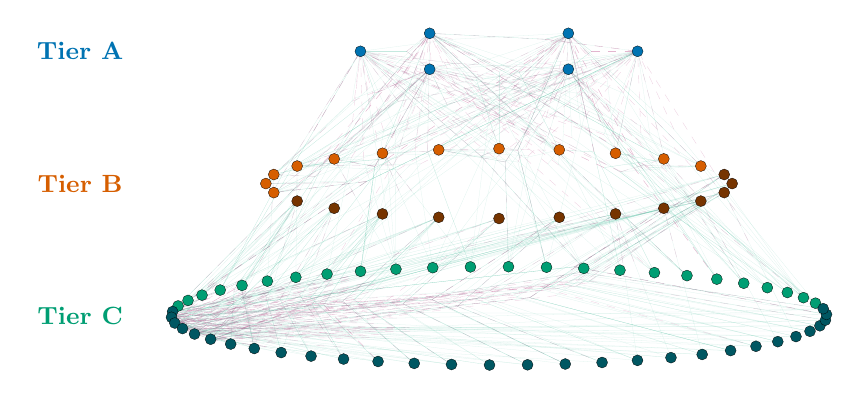
\begin{tikzpicture}[scale=1.4]
  \definecolor{slotin}{rgb}{0.000,0.620,0.450}
  \definecolor{slotout}{rgb}{0.800,0.470,0.650}
  \draw[slotin, line width=0.10pt, opacity=0.12] (1.257,1.200) -- (0.419,1.309);
  \draw[slotin, line width=0.10pt, opacity=0.12] (0.629,1.363) -- (0.419,1.309);
  \draw[slotout, line width=0.14pt, opacity=0.32, dashed] (0.419,1.309) -- (-0.629,1.363);
  \draw[slotin, line width=0.10pt, opacity=0.12] (1.257,1.200) -- (0.419,1.091);
  \draw[slotin, line width=0.10pt, opacity=0.12] (-0.629,1.037) -- (0.419,1.091);
  \draw[slotout, line width=0.14pt, opacity=0.32, dashed] (0.419,1.091) -- (0.629,1.037);
  \draw[slotin, line width=0.10pt, opacity=0.12] (1.257,1.200) -- (1.191,0.892);
  \draw[slotin, line width=0.10pt, opacity=0.12] (1.057,0.275) -- (1.191,0.892);
  \draw[slotout, line width=0.14pt, opacity=0.32, dashed] (1.191,0.892) -- (1.257,1.200);
  \draw[slotin, line width=0.10pt, opacity=0.12] (1.257,1.200) -- (1.512,0.190);
  \draw[slotin, line width=0.10pt, opacity=0.12] (1.057,0.275) -- (1.512,0.190);
  \draw[slotout, line width=0.14pt, opacity=0.32, dashed] (1.512,0.190) -- (2.220,-0.904);
  \draw[slotin, line width=0.10pt, opacity=0.12] (1.257,1.200) -- (-0.143,0.946);
  \draw[slotin, line width=0.10pt, opacity=0.12] (-1.057,0.275) -- (-0.143,0.946);
  \draw[slotout, line width=0.14pt, opacity=0.32, dashed] (-0.143,0.946) -- (-0.629,1.363);
  \draw[slotin, line width=0.10pt, opacity=0.12] (1.257,1.200) -- (-0.401,0.907);
  \draw[slotin, line width=0.10pt, opacity=0.12] (-1.831,0.159) -- (-0.401,0.907);
  \draw[slotout, line width=0.14pt, opacity=0.32, dashed] (-0.401,0.907) -- (-0.629,1.363);
  \draw[slotin, line width=0.10pt, opacity=0.12] (1.257,1.200) -- (0.157,0.773);
  \draw[slotin, line width=0.10pt, opacity=0.12] (-2.043,-0.082) -- (0.157,0.773);
  \draw[slotout, line width=0.14pt, opacity=0.32, dashed] (0.157,0.773) -- (1.257,1.200);
  \draw[slotin, line width=0.10pt, opacity=0.12] (1.257,1.200) -- (-1.202,0.019);
  \draw[slotin, line width=0.10pt, opacity=0.12] (-2.043,-0.082) -- (-1.202,0.019);
  \draw[slotout, line width=0.14pt, opacity=0.32, dashed] (-1.202,0.019) -- (-2.821,-1.060);
  \draw[slotin, line width=0.10pt, opacity=0.12] (1.257,1.200) -- (1.369,0.444);
  \draw[slotin, line width=0.10pt, opacity=0.12] (2.220,-0.904) -- (1.369,0.444);
  \draw[slotout, line width=0.14pt, opacity=0.32, dashed] (1.369,0.444) -- (0.629,1.037);
  \draw[slotin, line width=0.10pt, opacity=0.12] (1.257,1.200) -- (0.428,0.600);
  \draw[slotin, line width=0.10pt, opacity=0.12] (-0.601,-0.763) -- (0.428,0.600);
  \draw[slotout, line width=0.14pt, opacity=0.32, dashed] (0.428,0.600) -- (0.629,1.363);
  \draw[slotin, line width=0.10pt, opacity=0.12] (1.257,1.200) -- (0.014,0.571);
  \draw[slotin, line width=0.10pt, opacity=0.12] (-1.843,-0.850) -- (0.014,0.571);
  \draw[slotout, line width=0.14pt, opacity=0.32, dashed] (0.014,0.571) -- (0.629,1.363);
  \draw[slotin, line width=0.10pt, opacity=0.12] (1.257,1.200) -- (-0.806,0.169);
  \draw[slotin, line width=0.10pt, opacity=0.12] (-1.843,-0.850) -- (-0.806,0.169);
  \draw[slotout, line width=0.14pt, opacity=0.32, dashed] (-0.806,0.169) -- (-1.831,0.159);
  \draw[slotin, line width=0.10pt, opacity=0.12] (1.257,1.200) -- (-1.202,0.019);
  \draw[slotin, line width=0.10pt, opacity=0.12] (-2.821,-1.060) -- (-1.202,0.019);
  \draw[slotout, line width=0.14pt, opacity=0.32, dashed] (-1.202,0.019) -- (-2.043,-0.082);
  \draw[slotin, line width=0.10pt, opacity=0.12] (0.629,1.363) -- (0.419,1.309);
  \draw[slotin, line width=0.10pt, opacity=0.12] (-0.629,1.363) -- (0.419,1.309);
  \draw[slotout, line width=0.14pt, opacity=0.32, dashed] (0.419,1.309) -- (1.257,1.200);
  \draw[slotin, line width=0.10pt, opacity=0.12] (0.629,1.363) -- (0.838,1.200);
  \draw[slotin, line width=0.10pt, opacity=0.12] (0.629,1.037) -- (0.838,1.200);
  \draw[slotout, line width=0.14pt, opacity=0.32, dashed] (0.838,1.200) -- (1.257,1.200);
  \draw[slotin, line width=0.10pt, opacity=0.12] (0.629,1.363) -- (0.401,0.907);
  \draw[slotin, line width=0.10pt, opacity=0.12] (1.831,0.159) -- (0.401,0.907);
  \draw[slotout, line width=0.14pt, opacity=0.32, dashed] (0.401,0.907) -- (-1.257,1.200);
  \draw[slotin, line width=0.10pt, opacity=0.12] (0.629,1.363) -- (0.000,1.015);
  \draw[slotin, line width=0.10pt, opacity=0.12] (0.000,0.317) -- (0.000,1.015);
  \draw[slotout, line width=0.14pt, opacity=0.32, dashed] (0.000,1.015) -- (-0.629,1.363);
  \draw[slotin, line width=0.10pt, opacity=0.12] (0.629,1.363) -- (0.237,1.011);
  \draw[slotin, line width=0.10pt, opacity=0.12] (-0.547,0.306) -- (0.237,1.011);
  \draw[slotout, line width=0.14pt, opacity=0.32, dashed] (0.237,1.011) -- (0.629,1.363);
  \draw[slotin, line width=0.10pt, opacity=0.12] (0.629,1.363) -- (0.018,0.907);
  \draw[slotin, line width=0.10pt, opacity=0.12] (-1.831,0.159) -- (0.018,0.907);
  \draw[slotout, line width=0.14pt, opacity=0.32, dashed] (0.018,0.907) -- (1.257,1.200);
  \draw[slotin, line width=0.10pt, opacity=0.12] (0.629,1.363) -- (-0.191,0.853);
  \draw[slotin, line width=0.10pt, opacity=0.12] (-1.831,0.159) -- (-0.191,0.853);
  \draw[slotout, line width=0.14pt, opacity=0.32, dashed] (-0.191,0.853) -- (0.629,1.037);
  \draw[slotin, line width=0.10pt, opacity=0.12] (0.629,1.363) -- (0.957,0.547);
  \draw[slotin, line width=0.10pt, opacity=0.12] (2.871,-1.085) -- (0.957,0.547);
  \draw[slotout, line width=0.14pt, opacity=0.32, dashed] (0.957,0.547) -- (-0.629,1.363);
  \draw[slotin, line width=0.10pt, opacity=0.12] (0.629,1.363) -- (0.785,0.647);
  \draw[slotin, line width=0.10pt, opacity=0.12] (1.097,-0.786) -- (0.785,0.647);
  \draw[slotout, line width=0.14pt, opacity=0.32, dashed] (0.785,0.647) -- (0.629,1.363);
  \draw[slotin, line width=0.10pt, opacity=0.12] (0.629,1.363) -- (0.772,0.601);
  \draw[slotin, line width=0.10pt, opacity=0.12] (0.431,-0.759) -- (0.772,0.601);
  \draw[slotout, line width=0.14pt, opacity=0.32, dashed] (0.772,0.601) -- (1.257,1.200);
  \draw[slotin, line width=0.10pt, opacity=0.12] (0.629,1.363) -- (0.171,0.304);
  \draw[slotin, line width=0.10pt, opacity=0.12] (0.431,-0.759) -- (0.171,0.304);
  \draw[slotout, line width=0.14pt, opacity=0.32, dashed] (0.171,0.304) -- (-0.547,0.306);
  \draw[slotin, line width=0.10pt, opacity=0.12] (0.629,1.363) -- (-0.101,0.526);
  \draw[slotin, line width=0.10pt, opacity=0.12] (-1.560,-0.821) -- (-0.101,0.526);
  \draw[slotout, line width=0.14pt, opacity=0.32, dashed] (-0.101,0.526) -- (0.629,1.037);
  \draw[slotin, line width=0.10pt, opacity=0.12] (-0.629,1.363) -- (0.419,1.309);
  \draw[slotin, line width=0.10pt, opacity=0.12] (0.629,1.363) -- (0.419,1.309);
  \draw[slotout, line width=0.14pt, opacity=0.32, dashed] (0.419,1.309) -- (1.257,1.200);
  \draw[slotin, line width=0.10pt, opacity=0.12] (-0.629,1.363) -- (-0.838,1.200);
  \draw[slotin, line width=0.10pt, opacity=0.12] (-1.257,1.200) -- (-0.838,1.200);
  \draw[slotout, line width=0.14pt, opacity=0.32, dashed] (-0.838,1.200) -- (-0.629,1.037);
  \draw[slotin, line width=0.10pt, opacity=0.12] (-0.629,1.363) -- (0.191,0.962);
  \draw[slotin, line width=0.10pt, opacity=0.12] (1.831,0.159) -- (0.191,0.962);
  \draw[slotout, line width=0.14pt, opacity=0.32, dashed] (0.191,0.962) -- (-0.629,1.363);
  \draw[slotin, line width=0.10pt, opacity=0.12] (-0.629,1.363) -- (0.182,1.011);
  \draw[slotin, line width=0.10pt, opacity=0.12] (0.547,0.306) -- (0.182,1.011);
  \draw[slotout, line width=0.14pt, opacity=0.32, dashed] (0.182,1.011) -- (0.629,1.363);
  \draw[slotin, line width=0.10pt, opacity=0.12] (-0.629,1.363) -- (0.541,0.278);
  \draw[slotin, line width=0.10pt, opacity=0.12] (0.547,0.306) -- (0.541,0.278);
  \draw[slotout, line width=0.14pt, opacity=0.32, dashed] (0.541,0.278) -- (1.705,-0.835);
  \draw[slotin, line width=0.10pt, opacity=0.12] (-0.629,1.363) -- (-0.772,1.000);
  \draw[slotin, line width=0.10pt, opacity=0.12] (-1.057,0.275) -- (-0.772,1.000);
  \draw[slotout, line width=0.14pt, opacity=0.32, dashed] (-0.772,1.000) -- (-0.629,1.363);
  \draw[slotin, line width=0.10pt, opacity=0.12] (-0.629,1.363) -- (-1.100,0.827);
  \draw[slotin, line width=0.10pt, opacity=0.12] (-2.043,0.082) -- (-1.100,0.827);
  \draw[slotout, line width=0.14pt, opacity=0.32, dashed] (-1.100,0.827) -- (-0.629,1.037);
  \draw[slotin, line width=0.10pt, opacity=0.12] (-0.629,1.363) -- (0.921,0.564);
  \draw[slotin, line width=0.10pt, opacity=0.12] (2.762,-1.035) -- (0.921,0.564);
  \draw[slotout, line width=0.14pt, opacity=0.32, dashed] (0.921,0.564) -- (0.629,1.363);
  \draw[slotin, line width=0.10pt, opacity=0.12] (-0.629,1.363) -- (1.322,0.162);
  \draw[slotin, line width=0.10pt, opacity=0.12] (2.762,-1.035) -- (1.322,0.162);
  \draw[slotout, line width=0.14pt, opacity=0.32, dashed] (1.322,0.162) -- (1.831,0.159);
  \draw[slotin, line width=0.10pt, opacity=0.12] (-0.629,1.363) -- (0.149,0.522);
  \draw[slotin, line width=0.10pt, opacity=0.12] (1.705,-0.835) -- (0.149,0.522);
  \draw[slotout, line width=0.14pt, opacity=0.32, dashed] (0.149,0.522) -- (-0.629,1.037);
  \draw[slotin, line width=0.10pt, opacity=0.12] (-0.629,1.363) -- (-0.086,0.657);
  \draw[slotin, line width=0.10pt, opacity=0.12] (-0.259,-0.756) -- (-0.086,0.657);
  \draw[slotout, line width=0.14pt, opacity=0.32, dashed] (-0.086,0.657) -- (0.629,1.363);
  \draw[slotin, line width=0.10pt, opacity=0.12] (-0.629,1.363) -- (-1.329,0.560);
  \draw[slotin, line width=0.10pt, opacity=0.12] (-2.101,-0.885) -- (-1.329,0.560);
  \draw[slotout, line width=0.14pt, opacity=0.32, dashed] (-1.329,0.560) -- (-1.257,1.200);
  \draw[slotin, line width=0.10pt, opacity=0.12] (-1.257,1.200) -- (-0.419,1.309);
  \draw[slotin, line width=0.10pt, opacity=0.12] (0.629,1.363) -- (-0.419,1.309);
  \draw[slotout, line width=0.14pt, opacity=0.32, dashed] (-0.419,1.309) -- (-0.629,1.363);
  \draw[slotin, line width=0.10pt, opacity=0.12] (-1.257,1.200) -- (-0.838,1.200);
  \draw[slotin, line width=0.10pt, opacity=0.12] (-0.629,1.037) -- (-0.838,1.200);
  \draw[slotout, line width=0.14pt, opacity=0.32, dashed] (-0.838,1.200) -- (-0.629,1.363);
  \draw[slotin, line width=0.10pt, opacity=0.12] (-1.257,1.200) -- (-0.446,0.957);
  \draw[slotin, line width=0.10pt, opacity=0.12] (0.547,0.306) -- (-0.446,0.957);
  \draw[slotout, line width=0.14pt, opacity=0.32, dashed] (-0.446,0.957) -- (-0.629,1.363);
  \draw[slotin, line width=0.10pt, opacity=0.12] (-1.257,1.200) -- (0.233,0.233);
  \draw[slotin, line width=0.10pt, opacity=0.12] (0.547,0.306) -- (0.233,0.233);
  \draw[slotout, line width=0.14pt, opacity=0.32, dashed] (0.233,0.233) -- (1.410,-0.808);
  \draw[slotin, line width=0.10pt, opacity=0.12] (-1.257,1.200) -- (-0.163,0.249);
  \draw[slotin, line width=0.10pt, opacity=0.12] (0.000,0.317) -- (-0.163,0.249);
  \draw[slotout, line width=0.14pt, opacity=0.32, dashed] (-0.163,0.249) -- (0.769,-0.769);
  \draw[slotin, line width=0.10pt, opacity=0.12] (-1.257,1.200) -- (-1.127,0.820);
  \draw[slotin, line width=0.10pt, opacity=0.12] (-1.495,0.224) -- (-1.127,0.820);
  \draw[slotout, line width=0.14pt, opacity=0.32, dashed] (-1.127,0.820) -- (-0.629,1.037);
  \draw[slotin, line width=0.10pt, opacity=0.12] (-1.257,1.200) -- (-1.334,0.746);
  \draw[slotin, line width=0.10pt, opacity=0.12] (-2.115,0.000) -- (-1.334,0.746);
  \draw[slotout, line width=0.14pt, opacity=0.32, dashed] (-1.334,0.746) -- (-0.629,1.037);
  \draw[slotin, line width=0.10pt, opacity=0.12] (-1.257,1.200) -- (0.261,0.585);
  \draw[slotin, line width=0.10pt, opacity=0.12] (1.410,-0.808) -- (0.261,0.585);
  \draw[slotout, line width=0.14pt, opacity=0.32, dashed] (0.261,0.585) -- (0.629,1.363);
  \draw[slotin, line width=0.10pt, opacity=0.12] (-1.257,1.200) -- (-0.158,0.476);
  \draw[slotin, line width=0.10pt, opacity=0.12] (1.410,-0.808) -- (-0.158,0.476);
  \draw[slotout, line width=0.14pt, opacity=0.32, dashed] (-0.158,0.476) -- (-0.629,1.037);
  \draw[slotin, line width=0.10pt, opacity=0.12] (-1.257,1.200) -- (-0.582,0.544);
  \draw[slotin, line width=0.10pt, opacity=0.12] (0.769,-0.769) -- (-0.582,0.544);
  \draw[slotout, line width=0.14pt, opacity=0.32, dashed] (-0.582,0.544) -- (-1.257,1.200);
  \draw[slotin, line width=0.10pt, opacity=0.12] (-1.257,1.200) -- (-1.150,0.541);
  \draw[slotin, line width=0.10pt, opacity=0.12] (-0.935,-0.777) -- (-1.150,0.541);
  \draw[slotout, line width=0.14pt, opacity=0.32, dashed] (-1.150,0.541) -- (-1.257,1.200);
  \draw[slotin, line width=0.10pt, opacity=0.12] (-1.257,1.200) -- (-1.681,0.478);
  \draw[slotin, line width=0.10pt, opacity=0.12] (-2.529,-0.966) -- (-1.681,0.478);
  \draw[slotout, line width=0.14pt, opacity=0.32, dashed] (-1.681,0.478) -- (-1.257,1.200);
  \draw[slotin, line width=0.10pt, opacity=0.12] (-1.257,1.200) -- (-1.967,0.078);
  \draw[slotin, line width=0.10pt, opacity=0.12] (-2.529,-0.966) -- (-1.967,0.078);
  \draw[slotout, line width=0.14pt, opacity=0.32, dashed] (-1.967,0.078) -- (-2.115,0.000);
  \draw[slotin, line width=0.10pt, opacity=0.12] (-0.629,1.037) -- (-0.419,1.091);
  \draw[slotin, line width=0.10pt, opacity=0.12] (-1.257,1.200) -- (-0.419,1.091);
  \draw[slotout, line width=0.14pt, opacity=0.32, dashed] (-0.419,1.091) -- (0.629,1.037);
  \draw[slotin, line width=0.10pt, opacity=0.12] (-0.629,1.037) -- (0.708,0.820);
  \draw[slotin, line width=0.10pt, opacity=0.12] (1.495,0.224) -- (0.708,0.820);
  \draw[slotout, line width=0.14pt, opacity=0.32, dashed] (0.708,0.820) -- (1.257,1.200);
  \draw[slotin, line width=0.10pt, opacity=0.12] (-0.629,1.037) -- (0.498,0.766);
  \draw[slotin, line width=0.10pt, opacity=0.12] (1.495,0.224) -- (0.498,0.766);
  \draw[slotout, line width=0.14pt, opacity=0.32, dashed] (0.498,0.766) -- (0.629,1.037);
  \draw[slotin, line width=0.10pt, opacity=0.12] (-0.629,1.037) -- (-0.918,0.766);
  \draw[slotin, line width=0.10pt, opacity=0.12] (-1.495,0.224) -- (-0.918,0.766);
  \draw[slotout, line width=0.14pt, opacity=0.32, dashed] (-0.918,0.766) -- (-0.629,1.037);
  \draw[slotin, line width=0.10pt, opacity=0.12] (-0.629,1.037) -- (-1.100,0.827);
  \draw[slotin, line width=0.10pt, opacity=0.12] (-2.043,0.082) -- (-1.100,0.827);
  \draw[slotout, line width=0.14pt, opacity=0.32, dashed] (-1.100,0.827) -- (-0.629,1.363);
  \draw[slotin, line width=0.10pt, opacity=0.12] (-0.629,1.037) -- (-0.471,0.718);
  \draw[slotin, line width=0.10pt, opacity=0.12] (-2.043,-0.082) -- (-0.471,0.718);
  \draw[slotout, line width=0.14pt, opacity=0.32, dashed] (-0.471,0.718) -- (1.257,1.200);
  \draw[slotin, line width=0.10pt, opacity=0.12] (-0.629,1.037) -- (-1.861,-0.052);
  \draw[slotin, line width=0.10pt, opacity=0.12] (-2.043,-0.082) -- (-1.861,-0.052);
  \draw[slotout, line width=0.14pt, opacity=0.32, dashed] (-1.861,-0.052) -- (-2.911,-1.110);
  \draw[slotin, line width=0.10pt, opacity=0.12] (-0.629,1.037) -- (0.392,0.376);
  \draw[slotin, line width=0.10pt, opacity=0.12] (2.434,-0.944) -- (0.392,0.376);
  \draw[slotout, line width=0.14pt, opacity=0.32, dashed] (0.392,0.376) -- (-0.629,1.037);
  \draw[slotin, line width=0.10pt, opacity=0.12] (-0.629,1.037) -- (-1.047,0.480);
  \draw[slotin, line width=0.10pt, opacity=0.12] (-1.256,-0.796) -- (-1.047,0.480);
  \draw[slotout, line width=0.14pt, opacity=0.32, dashed] (-1.047,0.480) -- (-1.257,1.200);
  \draw[slotin, line width=0.10pt, opacity=0.12] (-0.629,1.037) -- (-1.127,0.155);
  \draw[slotin, line width=0.10pt, opacity=0.12] (-1.256,-0.796) -- (-1.127,0.155);
  \draw[slotout, line width=0.14pt, opacity=0.32, dashed] (-1.127,0.155) -- (-1.495,0.224);
  \draw[slotin, line width=0.10pt, opacity=0.12] (-0.629,1.037) -- (-1.668,0.065);
  \draw[slotin, line width=0.10pt, opacity=0.12] (-2.331,-0.924) -- (-1.668,0.065);
  \draw[slotout, line width=0.14pt, opacity=0.32, dashed] (-1.668,0.065) -- (-2.043,0.082);
  \draw[slotin, line width=0.10pt, opacity=0.12] (-0.629,1.037) -- (-0.970,0.321);
  \draw[slotin, line width=0.10pt, opacity=0.12] (-2.911,-1.110) -- (-0.970,0.321);
  \draw[slotout, line width=0.14pt, opacity=0.32, dashed] (-0.970,0.321) -- (0.629,1.037);
  \draw[slotin, line width=0.10pt, opacity=0.12] (0.629,1.037) -- (0.838,1.200);
  \draw[slotin, line width=0.10pt, opacity=0.12] (0.629,1.363) -- (0.838,1.200);
  \draw[slotout, line width=0.14pt, opacity=0.32, dashed] (0.838,1.200) -- (1.257,1.200);
  \draw[slotin, line width=0.10pt, opacity=0.12] (0.629,1.037) -- (-0.419,1.091);
  \draw[slotin, line width=0.10pt, opacity=0.12] (-0.629,1.037) -- (-0.419,1.091);
  \draw[slotout, line width=0.14pt, opacity=0.32, dashed] (-0.419,1.091) -- (-1.257,1.200);
  \draw[slotin, line width=0.10pt, opacity=0.12] (0.629,1.037) -- (0.498,0.766);
  \draw[slotin, line width=0.10pt, opacity=0.12] (1.495,0.224) -- (0.498,0.766);
  \draw[slotout, line width=0.14pt, opacity=0.32, dashed] (0.498,0.766) -- (-0.629,1.037);
  \draw[slotin, line width=0.10pt, opacity=0.12] (0.629,1.037) -- (0.772,0.892);
  \draw[slotin, line width=0.10pt, opacity=0.12] (1.057,0.275) -- (0.772,0.892);
  \draw[slotout, line width=0.14pt, opacity=0.32, dashed] (0.772,0.892) -- (0.629,1.363);
  \draw[slotin, line width=0.10pt, opacity=0.12] (0.629,1.037) -- (1.221,0.148);
  \draw[slotin, line width=0.10pt, opacity=0.12] (1.057,0.275) -- (1.221,0.148);
  \draw[slotout, line width=0.14pt, opacity=0.32, dashed] (1.221,0.148) -- (1.976,-0.867);
  \draw[slotin, line width=0.10pt, opacity=0.12] (0.629,1.037) -- (0.056,0.196);
  \draw[slotin, line width=0.10pt, opacity=0.12] (-0.547,0.306) -- (0.056,0.196);
  \draw[slotout, line width=0.14pt, opacity=0.32, dashed] (0.056,0.196) -- (0.086,-0.754);
  \draw[slotin, line width=0.10pt, opacity=0.12] (0.629,1.037) -- (-0.286,0.691);
  \draw[slotin, line width=0.10pt, opacity=0.12] (-2.115,0.000) -- (-0.286,0.691);
  \draw[slotout, line width=0.14pt, opacity=0.32, dashed] (-0.286,0.691) -- (0.629,1.037);
  \draw[slotin, line width=0.10pt, opacity=0.12] (0.629,1.037) -- (0.662,0.416);
  \draw[slotin, line width=0.10pt, opacity=0.12] (2.616,-0.988) -- (0.662,0.416);
  \draw[slotout, line width=0.14pt, opacity=0.32, dashed] (0.662,0.416) -- (-1.257,1.200);
  \draw[slotin, line width=0.10pt, opacity=0.12] (0.629,1.037) -- (1.287,0.457);
  \draw[slotin, line width=0.10pt, opacity=0.12] (1.976,-0.867) -- (1.287,0.457);
  \draw[slotout, line width=0.14pt, opacity=0.32, dashed] (1.287,0.457) -- (1.257,1.200);
  \draw[slotin, line width=0.10pt, opacity=0.12] (0.629,1.037) -- (1.078,0.402);
  \draw[slotin, line width=0.10pt, opacity=0.12] (1.976,-0.867) -- (1.078,0.402);
  \draw[slotout, line width=0.14pt, opacity=0.32, dashed] (1.078,0.402) -- (0.629,1.037);
  \draw[slotin, line width=0.10pt, opacity=0.12] (0.629,1.037) -- (0.448,0.440);
  \draw[slotin, line width=0.10pt, opacity=0.12] (0.086,-0.754) -- (0.448,0.440);
  \draw[slotout, line width=0.14pt, opacity=0.32, dashed] (0.448,0.440) -- (0.629,1.037);
  \draw[slotin, line width=0.10pt, opacity=0.12] (0.629,1.037) -- (-0.898,0.354);
  \draw[slotin, line width=0.10pt, opacity=0.12] (-2.694,-1.012) -- (-0.898,0.354);
  \draw[slotout, line width=0.14pt, opacity=0.32, dashed] (-0.898,0.354) -- (-0.629,1.037);
  \draw[slotin, line width=0.10pt, opacity=0.12] (1.831,0.159) -- (1.030,0.962);
  \draw[slotin, line width=0.10pt, opacity=0.12] (0.629,1.363) -- (1.030,0.962);
  \draw[slotout, line width=0.14pt, opacity=0.32, dashed] (1.030,0.962) -- (0.629,1.363);
  \draw[slotin, line width=0.10pt, opacity=0.12] (1.831,0.159) -- (1.430,0.560);
  \draw[slotin, line width=0.10pt, opacity=0.12] (0.629,1.363) -- (1.430,0.560);
  \draw[slotout, line width=0.14pt, opacity=0.32, dashed] (1.430,0.560) -- (1.831,0.159);
  \draw[slotin, line width=0.10pt, opacity=0.12] (1.831,0.159) -- (0.610,0.962);
  \draw[slotin, line width=0.10pt, opacity=0.12] (-0.629,1.363) -- (0.610,0.962);
  \draw[slotout, line width=0.14pt, opacity=0.32, dashed] (0.610,0.962) -- (0.629,1.363);
  \draw[slotin, line width=0.10pt, opacity=0.12] (1.831,0.159) -- (1.322,0.162);
  \draw[slotin, line width=0.10pt, opacity=0.12] (-0.629,1.363) -- (1.322,0.162);
  \draw[slotout, line width=0.14pt, opacity=0.32, dashed] (1.322,0.162) -- (2.762,-1.035);
  \draw[slotin, line width=0.10pt, opacity=0.12] (1.831,0.159) -- (1.358,0.146);
  \draw[slotin, line width=0.10pt, opacity=0.12] (2.871,-1.085) -- (1.358,0.146);
  \draw[slotout, line width=0.14pt, opacity=0.32, dashed] (1.358,0.146) -- (-0.629,1.363);
  \draw[slotin, line width=0.10pt, opacity=0.12] (1.831,0.159) -- (1.741,0.162);
  \draw[slotin, line width=0.10pt, opacity=0.12] (2.762,-1.035) -- (1.741,0.162);
  \draw[slotout, line width=0.14pt, opacity=0.32, dashed] (1.741,0.162) -- (0.629,1.363);
  \draw[slotin, line width=0.10pt, opacity=0.12] (1.831,0.159) -- (2.142,-0.239);
  \draw[slotin, line width=0.10pt, opacity=0.12] (2.762,-1.035) -- (2.142,-0.239);
  \draw[slotout, line width=0.14pt, opacity=0.32, dashed] (2.142,-0.239) -- (1.831,0.159);
  \draw[slotin, line width=0.10pt, opacity=0.12] (1.495,0.224) -- (0.498,0.766);
  \draw[slotin, line width=0.10pt, opacity=0.12] (-0.629,1.037) -- (0.498,0.766);
  \draw[slotout, line width=0.14pt, opacity=0.32, dashed] (0.498,0.766) -- (0.629,1.037);
  \draw[slotin, line width=0.10pt, opacity=0.12] (1.495,0.224) -- (1.127,0.820);
  \draw[slotin, line width=0.10pt, opacity=0.12] (0.629,1.037) -- (1.127,0.820);
  \draw[slotout, line width=0.14pt, opacity=0.32, dashed] (1.127,0.820) -- (1.257,1.200);
  \draw[slotin, line width=0.10pt, opacity=0.12] (1.495,0.224) -- (0.918,0.766);
  \draw[slotin, line width=0.10pt, opacity=0.12] (0.629,1.037) -- (0.918,0.766);
  \draw[slotout, line width=0.14pt, opacity=0.32, dashed] (0.918,0.766) -- (0.629,1.037);
  \draw[slotin, line width=0.10pt, opacity=0.12] (1.495,0.224) -- (0.951,0.145);
  \draw[slotin, line width=0.10pt, opacity=0.12] (2.616,-0.988) -- (0.951,0.145);
  \draw[slotout, line width=0.14pt, opacity=0.32, dashed] (0.951,0.145) -- (-1.257,1.200);
  \draw[slotin, line width=0.10pt, opacity=0.12] (1.495,0.224) -- (1.869,-0.180);
  \draw[slotin, line width=0.10pt, opacity=0.12] (2.616,-0.988) -- (1.869,-0.180);
  \draw[slotout, line width=0.14pt, opacity=0.32, dashed] (1.869,-0.180) -- (1.495,0.224);
  \draw[slotin, line width=0.10pt, opacity=0.12] (1.495,0.224) -- (1.519,0.106);
  \draw[slotin, line width=0.10pt, opacity=0.12] (2.434,-0.944) -- (1.519,0.106);
  \draw[slotout, line width=0.14pt, opacity=0.32, dashed] (1.519,0.106) -- (0.629,1.037);
  \draw[slotin, line width=0.10pt, opacity=0.12] (1.057,0.275) -- (0.981,0.946);
  \draw[slotin, line width=0.10pt, opacity=0.12] (1.257,1.200) -- (0.981,0.946);
  \draw[slotout, line width=0.14pt, opacity=0.32, dashed] (0.981,0.946) -- (0.629,1.363);
  \draw[slotin, line width=0.10pt, opacity=0.12] (1.057,0.275) -- (1.124,0.583);
  \draw[slotin, line width=0.10pt, opacity=0.12] (1.257,1.200) -- (1.124,0.583);
  \draw[slotout, line width=0.14pt, opacity=0.32, dashed] (1.124,0.583) -- (1.057,0.275);
  \draw[slotin, line width=0.10pt, opacity=0.12] (1.057,0.275) -- (0.352,0.783);
  \draw[slotin, line width=0.10pt, opacity=0.12] (0.629,1.037) -- (0.352,0.783);
  \draw[slotout, line width=0.14pt, opacity=0.32, dashed] (0.352,0.783) -- (-0.629,1.037);
  \draw[slotin, line width=0.10pt, opacity=0.12] (1.057,0.275) -- (1.221,0.148);
  \draw[slotin, line width=0.10pt, opacity=0.12] (0.629,1.037) -- (1.221,0.148);
  \draw[slotout, line width=0.14pt, opacity=0.32, dashed] (1.221,0.148) -- (1.976,-0.867);
  \draw[slotin, line width=0.10pt, opacity=0.12] (1.057,0.275) -- (1.302,0.136);
  \draw[slotin, line width=0.10pt, opacity=0.12] (2.220,-0.904) -- (1.302,0.136);
  \draw[slotout, line width=0.14pt, opacity=0.32, dashed] (1.302,0.136) -- (0.629,1.037);
  \draw[slotin, line width=0.10pt, opacity=0.12] (1.057,0.275) -- (1.221,0.257);
  \draw[slotin, line width=0.10pt, opacity=0.12] (1.976,-0.867) -- (1.221,0.257);
  \draw[slotout, line width=0.14pt, opacity=0.32, dashed] (1.221,0.257) -- (0.629,1.363);
  \draw[slotin, line width=0.10pt, opacity=0.12] (0.547,0.306) -- (0.182,1.011);
  \draw[slotin, line width=0.10pt, opacity=0.12] (-0.629,1.363) -- (0.182,1.011);
  \draw[slotout, line width=0.14pt, opacity=0.32, dashed] (0.182,1.011) -- (0.629,1.363);
  \draw[slotin, line width=0.10pt, opacity=0.12] (0.547,0.306) -- (-0.237,0.902);
  \draw[slotin, line width=0.10pt, opacity=0.12] (-0.629,1.363) -- (-0.237,0.902);
  \draw[slotout, line width=0.14pt, opacity=0.32, dashed] (-0.237,0.902) -- (-0.629,1.037);
  \draw[slotin, line width=0.10pt, opacity=0.12] (0.547,0.306) -- (-0.027,0.957);
  \draw[slotin, line width=0.10pt, opacity=0.12] (-1.257,1.200) -- (-0.027,0.957);
  \draw[slotout, line width=0.14pt, opacity=0.32, dashed] (-0.027,0.957) -- (0.629,1.363);
  \draw[slotin, line width=0.10pt, opacity=0.12] (0.547,0.306) -- (-0.054,0.604);
  \draw[slotin, line width=0.10pt, opacity=0.12] (-1.257,1.200) -- (-0.054,0.604);
  \draw[slotout, line width=0.14pt, opacity=0.32, dashed] (-0.054,0.604) -- (0.547,0.306);
  \draw[slotin, line width=0.10pt, opacity=0.12] (0.547,0.306) -- (0.541,0.278);
  \draw[slotin, line width=0.10pt, opacity=0.12] (1.705,-0.835) -- (0.541,0.278);
  \draw[slotout, line width=0.14pt, opacity=0.32, dashed] (0.541,0.278) -- (-0.629,1.363);
  \draw[slotin, line width=0.10pt, opacity=0.12] (0.547,0.306) -- (0.862,0.287);
  \draw[slotin, line width=0.10pt, opacity=0.12] (1.410,-0.808) -- (0.862,0.287);
  \draw[slotout, line width=0.14pt, opacity=0.32, dashed] (0.862,0.287) -- (0.629,1.363);
  \draw[slotin, line width=0.10pt, opacity=0.12] (0.547,0.306) -- (0.443,0.178);
  \draw[slotin, line width=0.10pt, opacity=0.12] (1.410,-0.808) -- (0.443,0.178);
  \draw[slotout, line width=0.14pt, opacity=0.32, dashed] (0.443,0.178) -- (-0.629,1.037);
  \draw[slotin, line width=0.10pt, opacity=0.12] (0.000,0.317) -- (-0.210,0.960);
  \draw[slotin, line width=0.10pt, opacity=0.12] (0.629,1.363) -- (-0.210,0.960);
  \draw[slotout, line width=0.14pt, opacity=0.32, dashed] (-0.210,0.960) -- (-1.257,1.200);
  \draw[slotin, line width=0.10pt, opacity=0.12] (0.000,0.317) -- (-0.210,0.960);
  \draw[slotin, line width=0.10pt, opacity=0.12] (-1.257,1.200) -- (-0.210,0.960);
  \draw[slotout, line width=0.14pt, opacity=0.32, dashed] (-0.210,0.960) -- (0.629,1.363);
  \draw[slotin, line width=0.10pt, opacity=0.12] (0.000,0.317) -- (-0.419,0.611);
  \draw[slotin, line width=0.10pt, opacity=0.12] (-1.257,1.200) -- (-0.419,0.611);
  \draw[slotout, line width=0.14pt, opacity=0.32, dashed] (-0.419,0.611) -- (0.000,0.317);
  \draw[slotin, line width=0.10pt, opacity=0.12] (0.000,0.317) -- (-0.053,0.244);
  \draw[slotin, line width=0.10pt, opacity=0.12] (1.097,-0.786) -- (-0.053,0.244);
  \draw[slotout, line width=0.14pt, opacity=0.32, dashed] (-0.053,0.244) -- (-1.257,1.200);
  \draw[slotin, line width=0.10pt, opacity=0.12] (0.000,0.317) -- (0.047,0.304);
  \draw[slotin, line width=0.10pt, opacity=0.12] (0.769,-0.769) -- (0.047,0.304);
  \draw[slotout, line width=0.14pt, opacity=0.32, dashed] (0.047,0.304) -- (-0.629,1.363);
  \draw[slotin, line width=0.10pt, opacity=0.12] (-0.547,0.306) -- (0.237,1.011);
  \draw[slotin, line width=0.10pt, opacity=0.12] (0.629,1.363) -- (0.237,1.011);
  \draw[slotout, line width=0.14pt, opacity=0.32, dashed] (0.237,1.011) -- (0.629,1.363);
  \draw[slotin, line width=0.10pt, opacity=0.12] (-0.547,0.306) -- (0.171,0.304);
  \draw[slotin, line width=0.10pt, opacity=0.12] (0.629,1.363) -- (0.171,0.304);
  \draw[slotout, line width=0.14pt, opacity=0.32, dashed] (0.171,0.304) -- (0.431,-0.759);
  \draw[slotin, line width=0.10pt, opacity=0.12] (-0.547,0.306) -- (0.237,0.793);
  \draw[slotin, line width=0.10pt, opacity=0.12] (0.629,1.037) -- (0.237,0.793);
  \draw[slotout, line width=0.14pt, opacity=0.32, dashed] (0.237,0.793) -- (0.629,1.037);
  \draw[slotin, line width=0.10pt, opacity=0.12] (-0.547,0.306) -- (0.171,0.304);
  \draw[slotin, line width=0.10pt, opacity=0.12] (0.431,-0.759) -- (0.171,0.304);
  \draw[slotout, line width=0.14pt, opacity=0.32, dashed] (0.171,0.304) -- (0.629,1.363);
  \draw[slotin, line width=0.10pt, opacity=0.12] (-0.547,0.306) -- (0.265,0.251);
  \draw[slotin, line width=0.10pt, opacity=0.12] (0.086,-0.754) -- (0.265,0.251);
  \draw[slotout, line width=0.14pt, opacity=0.32, dashed] (0.265,0.251) -- (1.257,1.200);
  \draw[slotin, line width=0.10pt, opacity=0.12] (-1.057,0.275) -- (0.486,0.892);
  \draw[slotin, line width=0.10pt, opacity=0.12] (1.257,1.200) -- (0.486,0.892);
  \draw[slotout, line width=0.14pt, opacity=0.32, dashed] (0.486,0.892) -- (1.257,1.200);
  \draw[slotin, line width=0.10pt, opacity=0.12] (-1.057,0.275) -- (-0.286,0.583);
  \draw[slotin, line width=0.10pt, opacity=0.12] (1.257,1.200) -- (-0.286,0.583);
  \draw[slotout, line width=0.14pt, opacity=0.32, dashed] (-0.286,0.583) -- (-1.057,0.275);
  \draw[slotin, line width=0.10pt, opacity=0.12] (-1.057,0.275) -- (-0.772,1.000);
  \draw[slotin, line width=0.10pt, opacity=0.12] (-0.629,1.363) -- (-0.772,1.000);
  \draw[slotout, line width=0.14pt, opacity=0.32, dashed] (-0.772,1.000) -- (-0.629,1.363);
  \draw[slotin, line width=0.10pt, opacity=0.12] (-1.057,0.275) -- (-0.020,0.240);
  \draw[slotin, line width=0.10pt, opacity=0.12] (-0.259,-0.756) -- (-0.020,0.240);
  \draw[slotout, line width=0.14pt, opacity=0.32, dashed] (-0.020,0.240) -- (1.257,1.200);
  \draw[slotin, line width=0.10pt, opacity=0.12] (-1.057,0.275) -- (-0.791,-0.069);
  \draw[slotin, line width=0.10pt, opacity=0.12] (-0.259,-0.756) -- (-0.791,-0.069);
  \draw[slotout, line width=0.14pt, opacity=0.32, dashed] (-0.791,-0.069) -- (-1.057,0.275);
  \draw[slotin, line width=0.10pt, opacity=0.12] (-1.057,0.275) -- (-0.905,-0.071);
  \draw[slotin, line width=0.10pt, opacity=0.12] (-0.601,-0.763) -- (-0.905,-0.071);
  \draw[slotout, line width=0.14pt, opacity=0.32, dashed] (-0.905,-0.071) -- (-1.057,0.275);
  \draw[slotin, line width=0.10pt, opacity=0.12] (-1.495,0.224) -- (-1.127,0.820);
  \draw[slotin, line width=0.10pt, opacity=0.12] (-1.257,1.200) -- (-1.127,0.820);
  \draw[slotout, line width=0.14pt, opacity=0.32, dashed] (-1.127,0.820) -- (-0.629,1.037);
  \draw[slotin, line width=0.10pt, opacity=0.12] (-1.495,0.224) -- (-0.918,0.875);
  \draw[slotin, line width=0.10pt, opacity=0.12] (-0.629,1.037) -- (-0.918,0.875);
  \draw[slotout, line width=0.14pt, opacity=0.32, dashed] (-0.918,0.875) -- (-0.629,1.363);
  \draw[slotin, line width=0.10pt, opacity=0.12] (-1.495,0.224) -- (-0.498,0.766);
  \draw[slotin, line width=0.10pt, opacity=0.12] (-0.629,1.037) -- (-0.498,0.766);
  \draw[slotout, line width=0.14pt, opacity=0.32, dashed] (-0.498,0.766) -- (0.629,1.037);
  \draw[slotin, line width=0.10pt, opacity=0.12] (-1.495,0.224) -- (-1.020,0.270);
  \draw[slotin, line width=0.10pt, opacity=0.12] (-0.935,-0.777) -- (-1.020,0.270);
  \draw[slotout, line width=0.14pt, opacity=0.32, dashed] (-1.020,0.270) -- (-0.629,1.363);
  \draw[slotin, line width=0.10pt, opacity=0.12] (-1.495,0.224) -- (-1.308,-0.109);
  \draw[slotin, line width=0.10pt, opacity=0.12] (-0.935,-0.777) -- (-1.308,-0.109);
  \draw[slotout, line width=0.14pt, opacity=0.32, dashed] (-1.308,-0.109) -- (-1.495,0.224);
  \draw[slotin, line width=0.10pt, opacity=0.12] (-1.495,0.224) -- (-1.127,0.155);
  \draw[slotin, line width=0.10pt, opacity=0.12] (-1.256,-0.796) -- (-1.127,0.155);
  \draw[slotout, line width=0.14pt, opacity=0.32, dashed] (-1.127,0.155) -- (-0.629,1.037);
  \draw[slotin, line width=0.10pt, opacity=0.12] (-1.831,0.159) -- (0.018,0.907);
  \draw[slotin, line width=0.10pt, opacity=0.12] (1.257,1.200) -- (0.018,0.907);
  \draw[slotout, line width=0.14pt, opacity=0.32, dashed] (0.018,0.907) -- (0.629,1.363);
  \draw[slotin, line width=0.10pt, opacity=0.12] (-1.831,0.159) -- (-0.802,0.506);
  \draw[slotin, line width=0.10pt, opacity=0.12] (1.257,1.200) -- (-0.802,0.506);
  \draw[slotout, line width=0.14pt, opacity=0.32, dashed] (-0.802,0.506) -- (-1.831,0.159);
  \draw[slotin, line width=0.10pt, opacity=0.12] (-1.831,0.159) -- (-0.610,0.962);
  \draw[slotin, line width=0.10pt, opacity=0.12] (0.629,1.363) -- (-0.610,0.962);
  \draw[slotout, line width=0.14pt, opacity=0.32, dashed] (-0.610,0.962) -- (-0.629,1.363);
  \draw[slotin, line width=0.10pt, opacity=0.12] (-1.831,0.159) -- (-0.921,0.234);
  \draw[slotin, line width=0.10pt, opacity=0.12] (0.629,1.363) -- (-0.921,0.234);
  \draw[slotout, line width=0.14pt, opacity=0.32, dashed] (-0.921,0.234) -- (-1.560,-0.821);
  \draw[slotin, line width=0.10pt, opacity=0.12] (-1.831,0.159) -- (-1.340,0.234);
  \draw[slotin, line width=0.10pt, opacity=0.12] (-1.560,-0.821) -- (-1.340,0.234);
  \draw[slotout, line width=0.14pt, opacity=0.32, dashed] (-1.340,0.234) -- (-0.629,1.363);
  \draw[slotin, line width=0.10pt, opacity=0.12] (-1.831,0.159) -- (-1.015,0.224);
  \draw[slotin, line width=0.10pt, opacity=0.12] (-1.843,-0.850) -- (-1.015,0.224);
  \draw[slotout, line width=0.14pt, opacity=0.32, dashed] (-1.015,0.224) -- (0.629,1.363);
  \draw[slotin, line width=0.10pt, opacity=0.12] (-1.831,0.159) -- (-1.835,-0.178);
  \draw[slotin, line width=0.10pt, opacity=0.12] (-1.843,-0.850) -- (-1.835,-0.178);
  \draw[slotout, line width=0.14pt, opacity=0.32, dashed] (-1.835,-0.178) -- (-1.831,0.159);
  \draw[slotin, line width=0.10pt, opacity=0.12] (-2.043,0.082) -- (-1.571,0.509);
  \draw[slotin, line width=0.10pt, opacity=0.12] (-0.629,1.363) -- (-1.571,0.509);
  \draw[slotout, line width=0.14pt, opacity=0.32, dashed] (-1.571,0.509) -- (-2.043,0.082);
  \draw[slotin, line width=0.10pt, opacity=0.12] (-2.043,0.082) -- (-1.310,0.773);
  \draw[slotin, line width=0.10pt, opacity=0.12] (-0.629,1.037) -- (-1.310,0.773);
  \draw[slotout, line width=0.14pt, opacity=0.32, dashed] (-1.310,0.773) -- (-1.257,1.200);
  \draw[slotin, line width=0.10pt, opacity=0.12] (-2.043,0.082) -- (-1.591,0.187);
  \draw[slotin, line width=0.10pt, opacity=0.12] (-2.101,-0.885) -- (-1.591,0.187);
  \draw[slotout, line width=0.14pt, opacity=0.32, dashed] (-1.591,0.187) -- (-0.629,1.363);
  \draw[slotin, line width=0.10pt, opacity=0.12] (-2.043,0.082) -- (-2.062,-0.240);
  \draw[slotin, line width=0.10pt, opacity=0.12] (-2.101,-0.885) -- (-2.062,-0.240);
  \draw[slotout, line width=0.14pt, opacity=0.32, dashed] (-2.062,-0.240) -- (-2.043,0.082);
  \draw[slotin, line width=0.10pt, opacity=0.12] (-2.043,0.082) -- (-1.668,0.065);
  \draw[slotin, line width=0.10pt, opacity=0.12] (-2.331,-0.924) -- (-1.668,0.065);
  \draw[slotout, line width=0.14pt, opacity=0.32, dashed] (-1.668,0.065) -- (-0.629,1.037);
  \draw[slotin, line width=0.10pt, opacity=0.12] (-2.115,0.000) -- (-0.914,0.746);
  \draw[slotin, line width=0.10pt, opacity=0.12] (-1.257,1.200) -- (-0.914,0.746);
  \draw[slotout, line width=0.14pt, opacity=0.32, dashed] (-0.914,0.746) -- (0.629,1.037);
  \draw[slotin, line width=0.10pt, opacity=0.12] (-2.115,0.000) -- (-0.914,0.746);
  \draw[slotin, line width=0.10pt, opacity=0.12] (0.629,1.037) -- (-0.914,0.746);
  \draw[slotout, line width=0.14pt, opacity=0.32, dashed] (-0.914,0.746) -- (-1.257,1.200);
  \draw[slotin, line width=0.10pt, opacity=0.12] (-2.115,0.000) -- (-1.393,0.008);
  \draw[slotin, line width=0.10pt, opacity=0.12] (0.629,1.037) -- (-1.393,0.008);
  \draw[slotout, line width=0.14pt, opacity=0.32, dashed] (-1.393,0.008) -- (-2.694,-1.012);
  \draw[slotin, line width=0.10pt, opacity=0.12] (-2.115,0.000) -- (-1.338,0.024);
  \draw[slotin, line width=0.10pt, opacity=0.12] (-2.529,-0.966) -- (-1.338,0.024);
  \draw[slotout, line width=0.14pt, opacity=0.32, dashed] (-1.338,0.024) -- (0.629,1.037);
  \draw[slotin, line width=0.10pt, opacity=0.12] (-2.115,0.000) -- (-1.812,0.008);
  \draw[slotin, line width=0.10pt, opacity=0.12] (-2.694,-1.012) -- (-1.812,0.008);
  \draw[slotout, line width=0.14pt, opacity=0.32, dashed] (-1.812,0.008) -- (-0.629,1.037);
  \draw[slotin, line width=0.10pt, opacity=0.12] (-2.043,-0.082) -- (-0.471,0.718);
  \draw[slotin, line width=0.10pt, opacity=0.12] (1.257,1.200) -- (-0.471,0.718);
  \draw[slotout, line width=0.14pt, opacity=0.32, dashed] (-0.471,0.718) -- (-0.629,1.037);
  \draw[slotin, line width=0.10pt, opacity=0.12] (-2.043,-0.082) -- (-1.202,0.019);
  \draw[slotin, line width=0.10pt, opacity=0.12] (1.257,1.200) -- (-1.202,0.019);
  \draw[slotout, line width=0.14pt, opacity=0.32, dashed] (-1.202,0.019) -- (-2.821,-1.060);
  \draw[slotin, line width=0.10pt, opacity=0.12] (-2.043,-0.082) -- (-1.571,0.291);
  \draw[slotin, line width=0.10pt, opacity=0.12] (-0.629,1.037) -- (-1.571,0.291);
  \draw[slotout, line width=0.14pt, opacity=0.32, dashed] (-1.571,0.291) -- (-2.043,-0.082);
  \draw[slotin, line width=0.10pt, opacity=0.12] (-2.043,-0.082) -- (-1.831,-0.035);
  \draw[slotin, line width=0.10pt, opacity=0.12] (-2.821,-1.060) -- (-1.831,-0.035);
  \draw[slotout, line width=0.14pt, opacity=0.32, dashed] (-1.831,-0.035) -- (-0.629,1.037);
  \draw[slotin, line width=0.10pt, opacity=0.12] (-2.043,-0.082) -- (-1.861,-0.052);
  \draw[slotin, line width=0.10pt, opacity=0.12] (-2.911,-1.110) -- (-1.861,-0.052);
  \draw[slotout, line width=0.14pt, opacity=0.32, dashed] (-1.861,-0.052) -- (-0.629,1.037);
  \draw[slotin, line width=0.10pt, opacity=0.12] (2.871,-1.085) -- (1.586,0.493);
  \draw[slotin, line width=0.10pt, opacity=0.12] (0.629,1.363) -- (1.586,0.493);
  \draw[slotout, line width=0.14pt, opacity=0.32, dashed] (1.586,0.493) -- (1.257,1.200);
  \draw[slotin, line width=0.10pt, opacity=0.12] (2.871,-1.085) -- (0.747,0.493);
  \draw[slotin, line width=0.10pt, opacity=0.12] (0.629,1.363) -- (0.747,0.493);
  \draw[slotout, line width=0.14pt, opacity=0.32, dashed] (0.747,0.493) -- (-1.257,1.200);
  \draw[slotin, line width=0.10pt, opacity=0.12] (2.871,-1.085) -- (1.358,0.146);
  \draw[slotin, line width=0.10pt, opacity=0.12] (1.831,0.159) -- (1.358,0.146);
  \draw[slotout, line width=0.14pt, opacity=0.32, dashed] (1.358,0.146) -- (-0.629,1.363);
  \draw[slotin, line width=0.10pt, opacity=0.12] (2.762,-1.035) -- (0.921,0.564);
  \draw[slotin, line width=0.10pt, opacity=0.12] (-0.629,1.363) -- (0.921,0.564);
  \draw[slotout, line width=0.14pt, opacity=0.32, dashed] (0.921,0.564) -- (0.629,1.363);
  \draw[slotin, line width=0.10pt, opacity=0.12] (2.762,-1.035) -- (1.950,0.108);
  \draw[slotin, line width=0.10pt, opacity=0.12] (1.831,0.159) -- (1.950,0.108);
  \draw[slotout, line width=0.14pt, opacity=0.32, dashed] (1.950,0.108) -- (1.257,1.200);
  \draw[slotin, line width=0.10pt, opacity=0.12] (2.762,-1.035) -- (1.112,0.108);
  \draw[slotin, line width=0.10pt, opacity=0.12] (1.831,0.159) -- (1.112,0.108);
  \draw[slotout, line width=0.14pt, opacity=0.32, dashed] (1.112,0.108) -- (-1.257,1.200);
  \draw[slotin, line width=0.10pt, opacity=0.12] (2.616,-0.988) -- (1.291,0.362);
  \draw[slotin, line width=0.10pt, opacity=0.12] (0.629,1.037) -- (1.291,0.362);
  \draw[slotout, line width=0.14pt, opacity=0.32, dashed] (1.291,0.362) -- (0.629,1.037);
  \draw[slotin, line width=0.10pt, opacity=0.12] (2.616,-0.988) -- (0.951,0.145);
  \draw[slotin, line width=0.10pt, opacity=0.12] (1.495,0.224) -- (0.951,0.145);
  \draw[slotout, line width=0.14pt, opacity=0.32, dashed] (0.951,0.145) -- (-1.257,1.200);
  \draw[slotin, line width=0.10pt, opacity=0.12] (2.434,-0.944) -- (1.021,0.431);
  \draw[slotin, line width=0.10pt, opacity=0.12] (-0.629,1.037) -- (1.021,0.431);
  \draw[slotout, line width=0.14pt, opacity=0.32, dashed] (1.021,0.431) -- (1.257,1.200);
  \draw[slotin, line width=0.10pt, opacity=0.12] (2.434,-0.944) -- (1.100,0.106);
  \draw[slotin, line width=0.10pt, opacity=0.12] (-0.629,1.037) -- (1.100,0.106);
  \draw[slotout, line width=0.14pt, opacity=0.32, dashed] (1.100,0.106) -- (1.495,0.224);
  \draw[slotin, line width=0.10pt, opacity=0.12] (2.434,-0.944) -- (1.100,0.106);
  \draw[slotin, line width=0.10pt, opacity=0.12] (1.495,0.224) -- (1.100,0.106);
  \draw[slotout, line width=0.14pt, opacity=0.32, dashed] (1.100,0.106) -- (-0.629,1.037);
  \draw[slotin, line width=0.10pt, opacity=0.12] (2.220,-0.904) -- (0.950,0.444);
  \draw[slotin, line width=0.10pt, opacity=0.12] (1.257,1.200) -- (0.950,0.444);
  \draw[slotout, line width=0.14pt, opacity=0.32, dashed] (0.950,0.444) -- (-0.629,1.037);
  \draw[slotin, line width=0.10pt, opacity=0.12] (2.220,-0.904) -- (1.512,0.190);
  \draw[slotin, line width=0.10pt, opacity=0.12] (1.057,0.275) -- (1.512,0.190);
  \draw[slotout, line width=0.14pt, opacity=0.32, dashed] (1.512,0.190) -- (1.257,1.200);
  \draw[slotin, line width=0.10pt, opacity=0.12] (2.220,-0.904) -- (1.302,0.136);
  \draw[slotin, line width=0.10pt, opacity=0.12] (1.057,0.275) -- (1.302,0.136);
  \draw[slotout, line width=0.14pt, opacity=0.32, dashed] (1.302,0.136) -- (0.629,1.037);
  \draw[slotin, line width=0.10pt, opacity=0.12] (1.976,-0.867) -- (1.078,0.402);
  \draw[slotin, line width=0.10pt, opacity=0.12] (0.629,1.037) -- (1.078,0.402);
  \draw[slotout, line width=0.14pt, opacity=0.32, dashed] (1.078,0.402) -- (0.629,1.037);
  \draw[slotin, line width=0.10pt, opacity=0.12] (1.976,-0.867) -- (1.221,0.257);
  \draw[slotin, line width=0.10pt, opacity=0.12] (1.057,0.275) -- (1.221,0.257);
  \draw[slotout, line width=0.14pt, opacity=0.32, dashed] (1.221,0.257) -- (0.629,1.363);
  \draw[slotin, line width=0.10pt, opacity=0.12] (1.705,-0.835) -- (0.149,0.631);
  \draw[slotin, line width=0.10pt, opacity=0.12] (-0.629,1.363) -- (0.149,0.631);
  \draw[slotout, line width=0.14pt, opacity=0.32, dashed] (0.149,0.631) -- (-0.629,1.363);
  \draw[slotin, line width=0.10pt, opacity=0.12] (1.705,-0.835) -- (0.541,0.278);
  \draw[slotin, line width=0.10pt, opacity=0.12] (-0.629,1.363) -- (0.541,0.278);
  \draw[slotout, line width=0.14pt, opacity=0.32, dashed] (0.541,0.278) -- (0.547,0.306);
  \draw[slotin, line width=0.10pt, opacity=0.12] (1.705,-0.835) -- (0.541,0.169);
  \draw[slotin, line width=0.10pt, opacity=0.12] (0.547,0.306) -- (0.541,0.169);
  \draw[slotout, line width=0.14pt, opacity=0.32, dashed] (0.541,0.169) -- (-0.629,1.037);
  \draw[slotin, line width=0.10pt, opacity=0.12] (1.410,-0.808) -- (-0.368,0.531);
  \draw[slotin, line width=0.10pt, opacity=0.12] (-1.257,1.200) -- (-0.368,0.531);
  \draw[slotout, line width=0.14pt, opacity=0.32, dashed] (-0.368,0.531) -- (-1.257,1.200);
  \draw[slotin, line width=0.10pt, opacity=0.12] (1.410,-0.808) -- (0.862,0.287);
  \draw[slotin, line width=0.10pt, opacity=0.12] (0.547,0.306) -- (0.862,0.287);
  \draw[slotout, line width=0.14pt, opacity=0.32, dashed] (0.862,0.287) -- (0.629,1.363);
  \draw[slotin, line width=0.10pt, opacity=0.12] (1.097,-0.786) -- (0.785,0.647);
  \draw[slotin, line width=0.10pt, opacity=0.12] (0.629,1.363) -- (0.785,0.647);
  \draw[slotout, line width=0.14pt, opacity=0.32, dashed] (0.785,0.647) -- (0.629,1.363);
  \draw[slotin, line width=0.10pt, opacity=0.12] (1.097,-0.786) -- (0.575,0.298);
  \draw[slotin, line width=0.10pt, opacity=0.12] (0.629,1.363) -- (0.575,0.298);
  \draw[slotout, line width=0.14pt, opacity=0.32, dashed] (0.575,0.298) -- (0.000,0.317);
  \draw[slotin, line width=0.10pt, opacity=0.12] (0.769,-0.769) -- (0.047,0.598);
  \draw[slotin, line width=0.10pt, opacity=0.12] (-1.257,1.200) -- (0.047,0.598);
  \draw[slotout, line width=0.14pt, opacity=0.32, dashed] (0.047,0.598) -- (0.629,1.363);
  \draw[slotin, line width=0.10pt, opacity=0.12] (0.769,-0.769) -- (-0.163,0.249);
  \draw[slotin, line width=0.10pt, opacity=0.12] (-1.257,1.200) -- (-0.163,0.249);
  \draw[slotout, line width=0.14pt, opacity=0.32, dashed] (-0.163,0.249) -- (0.000,0.317);
  \draw[slotin, line width=0.10pt, opacity=0.12] (0.769,-0.769) -- (-0.163,0.249);
  \draw[slotin, line width=0.10pt, opacity=0.12] (0.000,0.317) -- (-0.163,0.249);
  \draw[slotout, line width=0.14pt, opacity=0.32, dashed] (-0.163,0.249) -- (-1.257,1.200);
  \draw[slotin, line width=0.10pt, opacity=0.12] (0.431,-0.759) -- (0.171,0.304);
  \draw[slotin, line width=0.10pt, opacity=0.12] (0.629,1.363) -- (0.171,0.304);
  \draw[slotout, line width=0.14pt, opacity=0.32, dashed] (0.171,0.304) -- (-0.547,0.306);
  \draw[slotin, line width=0.10pt, opacity=0.12] (0.431,-0.759) -- (0.171,0.195);
  \draw[slotin, line width=0.10pt, opacity=0.12] (-0.547,0.306) -- (0.171,0.195);
  \draw[slotout, line width=0.14pt, opacity=0.32, dashed] (0.171,0.195) -- (0.629,1.037);
  \draw[slotin, line width=0.10pt, opacity=0.12] (0.086,-0.754) -- (0.056,0.196);
  \draw[slotin, line width=0.10pt, opacity=0.12] (0.629,1.037) -- (0.056,0.196);
  \draw[slotout, line width=0.14pt, opacity=0.32, dashed] (0.056,0.196) -- (-0.547,0.306);
  \draw[slotin, line width=0.10pt, opacity=0.12] (0.086,-0.754) -- (0.056,0.196);
  \draw[slotin, line width=0.10pt, opacity=0.12] (-0.547,0.306) -- (0.056,0.196);
  \draw[slotout, line width=0.14pt, opacity=0.32, dashed] (0.056,0.196) -- (0.629,1.037);
  \draw[slotin, line width=0.10pt, opacity=0.12] (-0.259,-0.756) -- (-0.648,0.294);
  \draw[slotin, line width=0.10pt, opacity=0.12] (-0.629,1.363) -- (-0.648,0.294);
  \draw[slotout, line width=0.14pt, opacity=0.32, dashed] (-0.648,0.294) -- (-1.057,0.275);
  \draw[slotin, line width=0.10pt, opacity=0.12] (-0.259,-0.756) -- (-0.648,0.294);
  \draw[slotin, line width=0.10pt, opacity=0.12] (-1.057,0.275) -- (-0.648,0.294);
  \draw[slotout, line width=0.14pt, opacity=0.32, dashed] (-0.648,0.294) -- (-0.629,1.363);
  \draw[slotin, line width=0.10pt, opacity=0.12] (-0.601,-0.763) -- (0.009,0.600);
  \draw[slotin, line width=0.10pt, opacity=0.12] (1.257,1.200) -- (0.009,0.600);
  \draw[slotout, line width=0.14pt, opacity=0.32, dashed] (0.009,0.600) -- (-0.629,1.363);
  \draw[slotin, line width=0.10pt, opacity=0.12] (-0.601,-0.763) -- (-0.762,0.292);
  \draw[slotin, line width=0.10pt, opacity=0.12] (-1.057,0.275) -- (-0.762,0.292);
  \draw[slotout, line width=0.14pt, opacity=0.32, dashed] (-0.762,0.292) -- (-0.629,1.363);
  \draw[slotin, line width=0.10pt, opacity=0.12] (-0.935,-0.777) -- (-0.940,0.487);
  \draw[slotin, line width=0.10pt, opacity=0.12] (-1.257,1.200) -- (-0.940,0.487);
  \draw[slotout, line width=0.14pt, opacity=0.32, dashed] (-0.940,0.487) -- (-0.629,1.037);
  \draw[slotin, line width=0.10pt, opacity=0.12] (-0.935,-0.777) -- (-1.229,0.216);
  \draw[slotin, line width=0.10pt, opacity=0.12] (-1.495,0.224) -- (-1.229,0.216);
  \draw[slotout, line width=0.14pt, opacity=0.32, dashed] (-1.229,0.216) -- (-1.257,1.200);
  \draw[slotin, line width=0.10pt, opacity=0.12] (-1.256,-0.796) -- (-0.838,0.535);
  \draw[slotin, line width=0.10pt, opacity=0.12] (-0.629,1.037) -- (-0.838,0.535);
  \draw[slotout, line width=0.14pt, opacity=0.32, dashed] (-0.838,0.535) -- (-0.629,1.363);
  \draw[slotin, line width=0.10pt, opacity=0.12] (-1.256,-0.796) -- (-1.127,0.155);
  \draw[slotin, line width=0.10pt, opacity=0.12] (-0.629,1.037) -- (-1.127,0.155);
  \draw[slotout, line width=0.14pt, opacity=0.32, dashed] (-1.127,0.155) -- (-1.495,0.224);
  \draw[slotin, line width=0.10pt, opacity=0.12] (-1.256,-0.796) -- (-1.127,0.155);
  \draw[slotin, line width=0.10pt, opacity=0.12] (-1.495,0.224) -- (-1.127,0.155);
  \draw[slotout, line width=0.14pt, opacity=0.32, dashed] (-1.127,0.155) -- (-0.629,1.037);
  \draw[slotin, line width=0.10pt, opacity=0.12] (-1.560,-0.821) -- (-0.101,0.635);
  \draw[slotin, line width=0.10pt, opacity=0.12] (0.629,1.363) -- (-0.101,0.635);
  \draw[slotout, line width=0.14pt, opacity=0.32, dashed] (-0.101,0.635) -- (0.629,1.363);
  \draw[slotin, line width=0.10pt, opacity=0.12] (-1.560,-0.821) -- (-0.711,0.179);
  \draw[slotin, line width=0.10pt, opacity=0.12] (-1.831,0.159) -- (-0.711,0.179);
  \draw[slotout, line width=0.14pt, opacity=0.32, dashed] (-0.711,0.179) -- (1.257,1.200);
  \draw[slotin, line width=0.10pt, opacity=0.12] (-1.560,-0.821) -- (-0.921,0.125);
  \draw[slotin, line width=0.10pt, opacity=0.12] (-1.831,0.159) -- (-0.921,0.125);
  \draw[slotout, line width=0.14pt, opacity=0.32, dashed] (-0.921,0.125) -- (0.629,1.037);
  \draw[slotin, line width=0.10pt, opacity=0.12] (-1.843,-0.850) -- (0.014,0.462);
  \draw[slotin, line width=0.10pt, opacity=0.12] (1.257,1.200) -- (0.014,0.462);
  \draw[slotout, line width=0.14pt, opacity=0.32, dashed] (0.014,0.462) -- (0.629,1.037);
  \draw[slotin, line width=0.10pt, opacity=0.12] (-1.843,-0.850) -- (-1.015,0.224);
  \draw[slotin, line width=0.10pt, opacity=0.12] (-1.831,0.159) -- (-1.015,0.224);
  \draw[slotout, line width=0.14pt, opacity=0.32, dashed] (-1.015,0.224) -- (0.629,1.363);
  \draw[slotin, line width=0.10pt, opacity=0.12] (-2.101,-0.885) -- (-1.120,0.614);
  \draw[slotin, line width=0.10pt, opacity=0.12] (-0.629,1.363) -- (-1.120,0.614);
  \draw[slotout, line width=0.14pt, opacity=0.32, dashed] (-1.120,0.614) -- (-0.629,1.363);
  \draw[slotin, line width=0.10pt, opacity=0.12] (-2.101,-0.885) -- (-1.591,0.187);
  \draw[slotin, line width=0.10pt, opacity=0.12] (-2.043,0.082) -- (-1.591,0.187);
  \draw[slotout, line width=0.14pt, opacity=0.32, dashed] (-1.591,0.187) -- (-0.629,1.363);
  \draw[slotin, line width=0.10pt, opacity=0.12] (-2.331,-0.924) -- (-1.196,0.492);
  \draw[slotin, line width=0.10pt, opacity=0.12] (-0.629,1.037) -- (-1.196,0.492);
  \draw[slotout, line width=0.14pt, opacity=0.32, dashed] (-1.196,0.492) -- (-0.629,1.363);
  \draw[slotin, line width=0.10pt, opacity=0.12] (-2.331,-0.924) -- (-1.668,0.174);
  \draw[slotin, line width=0.10pt, opacity=0.12] (-2.043,0.082) -- (-1.668,0.174);
  \draw[slotout, line width=0.14pt, opacity=0.32, dashed] (-1.668,0.174) -- (-0.629,1.363);
  \draw[slotin, line width=0.10pt, opacity=0.12] (-2.529,-0.966) -- (-1.681,0.478);
  \draw[slotin, line width=0.10pt, opacity=0.12] (-1.257,1.200) -- (-1.681,0.478);
  \draw[slotout, line width=0.14pt, opacity=0.32, dashed] (-1.681,0.478) -- (-1.257,1.200);
  \draw[slotin, line width=0.10pt, opacity=0.12] (-2.529,-0.966) -- (-1.967,0.078);
  \draw[slotin, line width=0.10pt, opacity=0.12] (-2.115,0.000) -- (-1.967,0.078);
  \draw[slotout, line width=0.14pt, opacity=0.32, dashed] (-1.967,0.078) -- (-1.257,1.200);
  \draw[slotin, line width=0.10pt, opacity=0.12] (-2.694,-1.012) -- (-1.107,0.408);
  \draw[slotin, line width=0.10pt, opacity=0.12] (0.629,1.037) -- (-1.107,0.408);
  \draw[slotout, line width=0.14pt, opacity=0.32, dashed] (-1.107,0.408) -- (-1.257,1.200);
  \draw[slotin, line width=0.10pt, opacity=0.12] (-2.694,-1.012) -- (-1.393,0.008);
  \draw[slotin, line width=0.10pt, opacity=0.12] (0.629,1.037) -- (-1.393,0.008);
  \draw[slotout, line width=0.14pt, opacity=0.32, dashed] (-1.393,0.008) -- (-2.115,0.000);
  \draw[slotin, line width=0.10pt, opacity=0.12] (-2.821,-1.060) -- (-0.102,0.447);
  \draw[slotin, line width=0.10pt, opacity=0.12] (1.257,1.200) -- (-0.102,0.447);
  \draw[slotout, line width=0.14pt, opacity=0.32, dashed] (-0.102,0.447) -- (1.257,1.200);
  \draw[slotin, line width=0.10pt, opacity=0.12] (-2.821,-1.060) -- (-1.202,0.019);
  \draw[slotin, line width=0.10pt, opacity=0.12] (1.257,1.200) -- (-1.202,0.019);
  \draw[slotout, line width=0.14pt, opacity=0.32, dashed] (-1.202,0.019) -- (-2.043,-0.082);
  \draw[slotin, line width=0.10pt, opacity=0.12] (-2.911,-1.110) -- (-0.761,0.376);
  \draw[slotin, line width=0.10pt, opacity=0.12] (-0.629,1.037) -- (-0.761,0.376);
  \draw[slotout, line width=0.14pt, opacity=0.32, dashed] (-0.761,0.376) -- (1.257,1.200);
  \draw[slotin, line width=0.10pt, opacity=0.12] (-2.911,-1.110) -- (-1.861,-0.052);
  \draw[slotin, line width=0.10pt, opacity=0.12] (-0.629,1.037) -- (-1.861,-0.052);
  \draw[slotout, line width=0.14pt, opacity=0.32, dashed] (-1.861,-0.052) -- (-2.043,-0.082);
  \draw[slotin, line width=0.10pt, opacity=0.12] (-2.961,-1.161) -- (-2.957,-1.213);
  \draw[slotin, line width=0.10pt, opacity=0.12] (-2.971,-1.213) -- (-2.957,-1.213);
  \draw[slotout, line width=0.14pt, opacity=0.32, dashed] (-2.957,-1.213) -- (-2.941,-1.265);
  \draw[slotin, line width=0.10pt, opacity=0.12] (-2.961,-1.161) -- (-2.780,-1.312);
  \draw[slotin, line width=0.10pt, opacity=0.12] (-2.762,-1.365) -- (-2.780,-1.312);
  \draw[slotout, line width=0.14pt, opacity=0.32, dashed] (-2.780,-1.312) -- (-2.616,-1.412);
  \draw[slotin, line width=0.10pt, opacity=0.12] (-2.961,-1.161) -- (-2.326,-0.866);
  \draw[slotin, line width=0.10pt, opacity=0.12] (-1.057,-0.275) -- (-2.326,-0.866);
  \draw[slotout, line width=0.14pt, opacity=0.32, dashed] (-2.326,-0.866) -- (-2.961,-1.161);
  \draw[slotin, line width=0.10pt, opacity=0.12] (-2.961,-1.161) -- (-1.809,-1.009);
  \draw[slotin, line width=0.10pt, opacity=0.12] (-1.057,-0.275) -- (-1.809,-1.009);
  \draw[slotout, line width=0.14pt, opacity=0.32, dashed] (-1.809,-1.009) -- (-1.410,-1.592);
  \draw[slotin, line width=0.10pt, opacity=0.12] (-2.961,-1.161) -- (-1.615,-0.900);
  \draw[slotin, line width=0.10pt, opacity=0.12] (1.057,-0.275) -- (-1.615,-0.900);
  \draw[slotout, line width=0.14pt, opacity=0.32, dashed] (-1.615,-0.900) -- (-2.941,-1.265);
  \draw[slotin, line width=0.10pt, opacity=0.12] (-2.961,-1.161) -- (-1.357,-0.861);
  \draw[slotin, line width=0.10pt, opacity=0.12] (1.831,-0.159) -- (-1.357,-0.861);
  \draw[slotout, line width=0.14pt, opacity=0.32, dashed] (-1.357,-0.861) -- (-2.941,-1.265);
  \draw[slotin, line width=0.10pt, opacity=0.12] (-2.961,-1.161) -- (-1.293,-0.747);
  \draw[slotin, line width=0.10pt, opacity=0.12] (2.043,0.082) -- (-1.293,-0.747);
  \draw[slotout, line width=0.14pt, opacity=0.32, dashed] (-1.293,-0.747) -- (-2.961,-1.161);
  \draw[slotin, line width=0.10pt, opacity=0.12] (-2.961,-1.161) -- (0.684,-0.755);
  \draw[slotin, line width=0.10pt, opacity=0.12] (2.043,0.082) -- (0.684,-0.755);
  \draw[slotout, line width=0.14pt, opacity=0.32, dashed] (0.684,-0.755) -- (2.971,-1.187);
  \draw[slotin, line width=0.10pt, opacity=0.12] (-2.961,-1.161) -- (-2.329,-1.388);
  \draw[slotin, line width=0.10pt, opacity=0.12] (-1.410,-1.592) -- (-2.329,-1.388);
  \draw[slotout, line width=0.14pt, opacity=0.32, dashed] (-2.329,-1.388) -- (-2.616,-1.412);
  \draw[slotin, line width=0.10pt, opacity=0.12] (-2.961,-1.161) -- (-1.457,-1.318);
  \draw[slotin, line width=0.10pt, opacity=0.12] (1.560,-1.579) -- (-1.457,-1.318);
  \draw[slotout, line width=0.14pt, opacity=0.32, dashed] (-1.457,-1.318) -- (-2.971,-1.213);
  \draw[slotin, line width=0.10pt, opacity=0.12] (-2.961,-1.161) -- (-1.134,-1.269);
  \draw[slotin, line width=0.10pt, opacity=0.12] (2.529,-1.434) -- (-1.134,-1.269);
  \draw[slotout, line width=0.14pt, opacity=0.32, dashed] (-1.134,-1.269) -- (-2.971,-1.213);
  \draw[slotin, line width=0.10pt, opacity=0.12] (-2.961,-1.161) -- (0.467,-0.918);
  \draw[slotin, line width=0.10pt, opacity=0.12] (2.529,-1.434) -- (0.467,-0.918);
  \draw[slotout, line width=0.14pt, opacity=0.32, dashed] (0.467,-0.918) -- (1.831,-0.159);
  \draw[slotin, line width=0.10pt, opacity=0.12] (-2.961,-1.161) -- (0.684,-0.755);
  \draw[slotin, line width=0.10pt, opacity=0.12] (2.971,-1.187) -- (0.684,-0.755);
  \draw[slotout, line width=0.14pt, opacity=0.32, dashed] (0.684,-0.755) -- (2.043,0.082);
  \draw[slotin, line width=0.10pt, opacity=0.12] (-2.971,-1.213) -- (-2.957,-1.213);
  \draw[slotin, line width=0.10pt, opacity=0.12] (-2.941,-1.265) -- (-2.957,-1.213);
  \draw[slotout, line width=0.14pt, opacity=0.32, dashed] (-2.957,-1.213) -- (-2.961,-1.161);
  \draw[slotin, line width=0.10pt, opacity=0.12] (-2.971,-1.213) -- (-2.849,-1.262);
  \draw[slotin, line width=0.10pt, opacity=0.12] (-2.616,-1.412) -- (-2.849,-1.262);
  \draw[slotout, line width=0.14pt, opacity=0.32, dashed] (-2.849,-1.262) -- (-2.961,-1.161);
  \draw[slotin, line width=0.10pt, opacity=0.12] (-2.971,-1.213) -- (-2.558,-0.896);
  \draw[slotin, line width=0.10pt, opacity=0.12] (-1.831,-0.159) -- (-2.558,-0.896);
  \draw[slotout, line width=0.14pt, opacity=0.32, dashed] (-2.558,-0.896) -- (-2.871,-1.315);
  \draw[slotin, line width=0.10pt, opacity=0.12] (-2.971,-1.213) -- (-1.970,-0.932);
  \draw[slotin, line width=0.10pt, opacity=0.12] (-0.000,-0.317) -- (-1.970,-0.932);
  \draw[slotout, line width=0.14pt, opacity=0.32, dashed] (-1.970,-0.932) -- (-2.941,-1.265);
  \draw[slotin, line width=0.10pt, opacity=0.12] (-2.971,-1.213) -- (-1.798,-0.911);
  \draw[slotin, line width=0.10pt, opacity=0.12] (0.547,-0.306) -- (-1.798,-0.911);
  \draw[slotout, line width=0.14pt, opacity=0.32, dashed] (-1.798,-0.911) -- (-2.971,-1.213);
  \draw[slotin, line width=0.10pt, opacity=0.12] (-2.971,-1.213) -- (-1.367,-0.844);
  \draw[slotin, line width=0.10pt, opacity=0.12] (1.831,-0.159) -- (-1.367,-0.844);
  \draw[slotout, line width=0.14pt, opacity=0.32, dashed] (-1.367,-0.844) -- (-2.961,-1.161);
  \draw[slotin, line width=0.10pt, opacity=0.12] (-2.971,-1.213) -- (-1.252,-0.928);
  \draw[slotin, line width=0.10pt, opacity=0.12] (1.831,-0.159) -- (-1.252,-0.928);
  \draw[slotout, line width=0.14pt, opacity=0.32, dashed] (-1.252,-0.928) -- (-2.616,-1.412);
  \draw[slotin, line width=0.10pt, opacity=0.12] (-2.971,-1.213) -- (-2.782,-1.311);
  \draw[slotin, line width=0.10pt, opacity=0.12] (-2.434,-1.456) -- (-2.782,-1.311);
  \draw[slotout, line width=0.14pt, opacity=0.32, dashed] (-2.782,-1.311) -- (-2.941,-1.265);
  \draw[slotin, line width=0.10pt, opacity=0.12] (-2.971,-1.213) -- (-2.009,-1.357);
  \draw[slotin, line width=0.10pt, opacity=0.12] (-0.086,-1.646) -- (-2.009,-1.357);
  \draw[slotout, line width=0.14pt, opacity=0.32, dashed] (-2.009,-1.357) -- (-2.971,-1.213);
  \draw[slotin, line width=0.10pt, opacity=0.12] (-2.971,-1.213) -- (-1.777,-1.337);
  \draw[slotin, line width=0.10pt, opacity=0.12] (0.601,-1.637) -- (-1.777,-1.337);
  \draw[slotout, line width=0.14pt, opacity=0.32, dashed] (-1.777,-1.337) -- (-2.961,-1.161);
  \draw[slotin, line width=0.10pt, opacity=0.12] (-2.971,-1.213) -- (-0.607,-1.052);
  \draw[slotin, line width=0.10pt, opacity=0.12] (0.601,-1.637) -- (-0.607,-1.052);
  \draw[slotout, line width=0.14pt, opacity=0.32, dashed] (-0.607,-1.052) -- (0.547,-0.306);
  \draw[slotin, line width=0.10pt, opacity=0.12] (-2.971,-1.213) -- (-1.085,-1.367);
  \draw[slotin, line width=0.10pt, opacity=0.12] (2.331,-1.476) -- (-1.085,-1.367);
  \draw[slotout, line width=0.14pt, opacity=0.32, dashed] (-1.085,-1.367) -- (-2.616,-1.412);
  \draw[slotin, line width=0.10pt, opacity=0.12] (-2.941,-1.265) -- (-2.957,-1.213);
  \draw[slotin, line width=0.10pt, opacity=0.12] (-2.971,-1.213) -- (-2.957,-1.213);
  \draw[slotout, line width=0.14pt, opacity=0.32, dashed] (-2.957,-1.213) -- (-2.961,-1.161);
  \draw[slotin, line width=0.10pt, opacity=0.12] (-2.941,-1.265) -- (-2.858,-1.315);
  \draw[slotin, line width=0.10pt, opacity=0.12] (-2.871,-1.315) -- (-2.858,-1.315);
  \draw[slotout, line width=0.14pt, opacity=0.32, dashed] (-2.858,-1.315) -- (-2.762,-1.365);
  \draw[slotin, line width=0.10pt, opacity=0.12] (-2.941,-1.265) -- (-2.571,-0.896);
  \draw[slotin, line width=0.10pt, opacity=0.12] (-1.831,-0.159) -- (-2.571,-0.896);
  \draw[slotout, line width=0.14pt, opacity=0.32, dashed] (-2.571,-0.896) -- (-2.941,-1.265);
  \draw[slotin, line width=0.10pt, opacity=0.12] (-2.941,-1.265) -- (-2.153,-0.928);
  \draw[slotin, line width=0.10pt, opacity=0.12] (-0.547,-0.306) -- (-2.153,-0.928);
  \draw[slotout, line width=0.14pt, opacity=0.32, dashed] (-2.153,-0.928) -- (-2.971,-1.213);
  \draw[slotin, line width=0.10pt, opacity=0.12] (-2.941,-1.265) -- (-1.419,-1.067);
  \draw[slotin, line width=0.10pt, opacity=0.12] (-0.547,-0.306) -- (-1.419,-1.067);
  \draw[slotout, line width=0.14pt, opacity=0.32, dashed] (-1.419,-1.067) -- (-0.769,-1.631);
  \draw[slotin, line width=0.10pt, opacity=0.12] (-2.941,-1.265) -- (-1.608,-0.935);
  \draw[slotin, line width=0.10pt, opacity=0.12] (1.057,-0.275) -- (-1.608,-0.935);
  \draw[slotout, line width=0.14pt, opacity=0.32, dashed] (-1.608,-0.935) -- (-2.941,-1.265);
  \draw[slotin, line width=0.10pt, opacity=0.12] (-2.941,-1.265) -- (-1.220,-0.904);
  \draw[slotin, line width=0.10pt, opacity=0.12] (2.043,-0.082) -- (-1.220,-0.904);
  \draw[slotout, line width=0.14pt, opacity=0.32, dashed] (-1.220,-0.904) -- (-2.762,-1.365);
  \draw[slotin, line width=0.10pt, opacity=0.12] (-2.941,-1.265) -- (-2.710,-1.325);
  \draw[slotin, line width=0.10pt, opacity=0.12] (-2.220,-1.496) -- (-2.710,-1.325);
  \draw[slotout, line width=0.14pt, opacity=0.32, dashed] (-2.710,-1.325) -- (-2.971,-1.213);
  \draw[slotin, line width=0.10pt, opacity=0.12] (-2.941,-1.265) -- (-2.331,-0.973);
  \draw[slotin, line width=0.10pt, opacity=0.12] (-2.220,-1.496) -- (-2.331,-0.973);
  \draw[slotout, line width=0.14pt, opacity=0.32, dashed] (-2.331,-0.973) -- (-1.831,-0.159);
  \draw[slotin, line width=0.10pt, opacity=0.12] (-2.941,-1.265) -- (-2.157,-1.420);
  \draw[slotin, line width=0.10pt, opacity=0.12] (-0.769,-1.631) -- (-2.157,-1.420);
  \draw[slotout, line width=0.14pt, opacity=0.32, dashed] (-2.157,-1.420) -- (-2.762,-1.365);
  \draw[slotin, line width=0.10pt, opacity=0.12] (-2.941,-1.265) -- (-1.552,-1.361);
  \draw[slotin, line width=0.10pt, opacity=0.12] (1.256,-1.604) -- (-1.552,-1.361);
  \draw[slotout, line width=0.14pt, opacity=0.32, dashed] (-1.552,-1.361) -- (-2.971,-1.213);
  \draw[slotin, line width=0.10pt, opacity=0.12] (-2.941,-1.265) -- (-1.039,-1.323);
  \draw[slotin, line width=0.10pt, opacity=0.12] (2.694,-1.388) -- (-1.039,-1.323);
  \draw[slotout, line width=0.14pt, opacity=0.32, dashed] (-1.039,-1.323) -- (-2.871,-1.315);
  \draw[slotin, line width=0.10pt, opacity=0.12] (-2.871,-1.315) -- (-2.927,-1.264);
  \draw[slotin, line width=0.10pt, opacity=0.12] (-2.971,-1.213) -- (-2.927,-1.264);
  \draw[slotout, line width=0.14pt, opacity=0.32, dashed] (-2.927,-1.264) -- (-2.941,-1.265);
  \draw[slotin, line width=0.10pt, opacity=0.12] (-2.871,-1.315) -- (-2.858,-1.315);
  \draw[slotin, line width=0.10pt, opacity=0.12] (-2.762,-1.365) -- (-2.858,-1.315);
  \draw[slotout, line width=0.14pt, opacity=0.32, dashed] (-2.858,-1.315) -- (-2.941,-1.265);
  \draw[slotin, line width=0.10pt, opacity=0.12] (-2.871,-1.315) -- (-2.120,-0.962);
  \draw[slotin, line width=0.10pt, opacity=0.12] (-0.547,-0.306) -- (-2.120,-0.962);
  \draw[slotout, line width=0.14pt, opacity=0.32, dashed] (-2.120,-0.962) -- (-2.941,-1.265);
  \draw[slotin, line width=0.10pt, opacity=0.12] (-2.871,-1.315) -- (-1.283,-1.088);
  \draw[slotin, line width=0.10pt, opacity=0.12] (-0.547,-0.306) -- (-1.283,-1.088);
  \draw[slotout, line width=0.14pt, opacity=0.32, dashed] (-1.283,-1.088) -- (-0.431,-1.641);
  \draw[slotin, line width=0.10pt, opacity=0.12] (-2.871,-1.315) -- (-0.871,-1.092);
  \draw[slotin, line width=0.10pt, opacity=0.12] (-0.000,-0.317) -- (-0.871,-1.092);
  \draw[slotout, line width=0.14pt, opacity=0.32, dashed] (-0.871,-1.092) -- (0.259,-1.644);
  \draw[slotin, line width=0.10pt, opacity=0.12] (-2.871,-1.315) -- (-1.379,-0.968);
  \draw[slotin, line width=0.10pt, opacity=0.12] (1.495,-0.224) -- (-1.379,-0.968);
  \draw[slotout, line width=0.14pt, opacity=0.32, dashed] (-1.379,-0.968) -- (-2.762,-1.365);
  \draw[slotin, line width=0.10pt, opacity=0.12] (-2.871,-1.315) -- (-1.173,-0.893);
  \draw[slotin, line width=0.10pt, opacity=0.12] (2.115,-0.000) -- (-1.173,-0.893);
  \draw[slotout, line width=0.14pt, opacity=0.32, dashed] (-1.173,-0.893) -- (-2.762,-1.365);
  \draw[slotin, line width=0.10pt, opacity=0.12] (-2.871,-1.315) -- (-2.091,-1.390);
  \draw[slotin, line width=0.10pt, opacity=0.12] (-0.431,-1.641) -- (-2.091,-1.390);
  \draw[slotout, line width=0.14pt, opacity=0.32, dashed] (-2.091,-1.390) -- (-2.971,-1.213);
  \draw[slotin, line width=0.10pt, opacity=0.12] (-2.871,-1.315) -- (-2.021,-1.440);
  \draw[slotin, line width=0.10pt, opacity=0.12] (-0.431,-1.641) -- (-2.021,-1.440);
  \draw[slotout, line width=0.14pt, opacity=0.32, dashed] (-2.021,-1.440) -- (-2.762,-1.365);
  \draw[slotin, line width=0.10pt, opacity=0.12] (-2.871,-1.315) -- (-1.827,-1.425);
  \draw[slotin, line width=0.10pt, opacity=0.12] (0.259,-1.644) -- (-1.827,-1.425);
  \draw[slotout, line width=0.14pt, opacity=0.32, dashed] (-1.827,-1.425) -- (-2.871,-1.315);
  \draw[slotin, line width=0.10pt, opacity=0.12] (-2.871,-1.315) -- (-1.299,-1.393);
  \draw[slotin, line width=0.10pt, opacity=0.12] (1.843,-1.550) -- (-1.299,-1.393);
  \draw[slotout, line width=0.14pt, opacity=0.32, dashed] (-1.299,-1.393) -- (-2.871,-1.315);
  \draw[slotin, line width=0.10pt, opacity=0.12] (-2.871,-1.315) -- (-0.944,-1.307);
  \draw[slotin, line width=0.10pt, opacity=0.12] (2.911,-1.290) -- (-0.944,-1.307);
  \draw[slotout, line width=0.14pt, opacity=0.32, dashed] (-0.944,-1.307) -- (-2.871,-1.315);
  \draw[slotin, line width=0.10pt, opacity=0.12] (-2.871,-1.315) -- (0.718,-0.869);
  \draw[slotin, line width=0.10pt, opacity=0.12] (2.911,-1.290) -- (0.718,-0.869);
  \draw[slotout, line width=0.14pt, opacity=0.32, dashed] (0.718,-0.869) -- (2.115,-0.000);
  \draw[slotin, line width=0.10pt, opacity=0.12] (-2.762,-1.365) -- (-2.750,-1.364);
  \draw[slotin, line width=0.10pt, opacity=0.12] (-2.871,-1.315) -- (-2.750,-1.364);
  \draw[slotout, line width=0.14pt, opacity=0.32, dashed] (-2.750,-1.364) -- (-2.616,-1.412);
  \draw[slotin, line width=0.10pt, opacity=0.12] (-2.762,-1.365) -- (-2.406,-0.917);
  \draw[slotin, line width=0.10pt, opacity=0.12] (-1.495,-0.224) -- (-2.406,-0.917);
  \draw[slotout, line width=0.14pt, opacity=0.32, dashed] (-2.406,-0.917) -- (-2.961,-1.161);
  \draw[slotin, line width=0.10pt, opacity=0.12] (-2.762,-1.365) -- (-2.291,-1.000);
  \draw[slotin, line width=0.10pt, opacity=0.12] (-1.495,-0.224) -- (-2.291,-1.000);
  \draw[slotout, line width=0.14pt, opacity=0.32, dashed] (-2.291,-1.000) -- (-2.616,-1.412);
  \draw[slotin, line width=0.10pt, opacity=0.12] (-2.762,-1.365) -- (-1.343,-0.984);
  \draw[slotin, line width=0.10pt, opacity=0.12] (1.495,-0.224) -- (-1.343,-0.984);
  \draw[slotout, line width=0.14pt, opacity=0.32, dashed] (-1.343,-0.984) -- (-2.762,-1.365);
  \draw[slotin, line width=0.10pt, opacity=0.12] (-2.762,-1.365) -- (-1.220,-0.904);
  \draw[slotin, line width=0.10pt, opacity=0.12] (2.043,-0.082) -- (-1.220,-0.904);
  \draw[slotout, line width=0.14pt, opacity=0.32, dashed] (-1.220,-0.904) -- (-2.941,-1.265);
  \draw[slotin, line width=0.10pt, opacity=0.12] (-2.762,-1.365) -- (-1.227,-0.815);
  \draw[slotin, line width=0.10pt, opacity=0.12] (2.043,0.082) -- (-1.227,-0.815);
  \draw[slotout, line width=0.14pt, opacity=0.32, dashed] (-1.227,-0.815) -- (-2.961,-1.161);
  \draw[slotin, line width=0.10pt, opacity=0.12] (-2.762,-1.365) -- (0.740,-0.806);
  \draw[slotin, line width=0.10pt, opacity=0.12] (2.043,0.082) -- (0.740,-0.806);
  \draw[slotout, line width=0.14pt, opacity=0.32, dashed] (0.740,-0.806) -- (2.941,-1.135);
  \draw[slotin, line width=0.10pt, opacity=0.12] (-2.762,-1.365) -- (-2.410,-1.431);
  \draw[slotin, line width=0.10pt, opacity=0.12] (-1.705,-1.565) -- (-2.410,-1.431);
  \draw[slotout, line width=0.14pt, opacity=0.32, dashed] (-2.410,-1.431) -- (-2.762,-1.365);
  \draw[slotin, line width=0.10pt, opacity=0.12] (-2.762,-1.365) -- (-1.177,-1.398);
  \draw[slotin, line width=0.10pt, opacity=0.12] (2.101,-1.515) -- (-1.177,-1.398);
  \draw[slotout, line width=0.14pt, opacity=0.32, dashed] (-1.177,-1.398) -- (-2.871,-1.315);
  \draw[slotin, line width=0.10pt, opacity=0.12] (-2.762,-1.365) -- (0.278,-1.035);
  \draw[slotin, line width=0.10pt, opacity=0.12] (2.101,-1.515) -- (0.278,-1.035);
  \draw[slotout, line width=0.14pt, opacity=0.32, dashed] (0.278,-1.035) -- (1.495,-0.224);
  \draw[slotin, line width=0.10pt, opacity=0.12] (-2.762,-1.365) -- (0.701,-0.929);
  \draw[slotin, line width=0.10pt, opacity=0.12] (2.821,-1.340) -- (0.701,-0.929);
  \draw[slotout, line width=0.14pt, opacity=0.32, dashed] (0.701,-0.929) -- (2.043,-0.082);
  \draw[slotin, line width=0.10pt, opacity=0.12] (-2.762,-1.365) -- (-0.812,-1.304);
  \draw[slotin, line width=0.10pt, opacity=0.12] (2.941,-1.135) -- (-0.812,-1.304);
  \draw[slotout, line width=0.14pt, opacity=0.32, dashed] (-0.812,-1.304) -- (-2.616,-1.412);
  \draw[slotin, line width=0.10pt, opacity=0.12] (-2.616,-1.412) -- (-2.849,-1.262);
  \draw[slotin, line width=0.10pt, opacity=0.12] (-2.971,-1.213) -- (-2.849,-1.262);
  \draw[slotout, line width=0.14pt, opacity=0.32, dashed] (-2.849,-1.262) -- (-2.961,-1.161);
  \draw[slotin, line width=0.10pt, opacity=0.12] (-2.616,-1.412) -- (-2.750,-1.364);
  \draw[slotin, line width=0.10pt, opacity=0.12] (-2.762,-1.365) -- (-2.750,-1.364);
  \draw[slotout, line width=0.14pt, opacity=0.32, dashed] (-2.750,-1.364) -- (-2.871,-1.315);
  \draw[slotin, line width=0.10pt, opacity=0.12] (-2.616,-1.412) -- (-2.291,-1.000);
  \draw[slotin, line width=0.10pt, opacity=0.12] (-1.495,-0.224) -- (-2.291,-1.000);
  \draw[slotout, line width=0.14pt, opacity=0.32, dashed] (-2.291,-1.000) -- (-2.762,-1.365);
  \draw[slotin, line width=0.10pt, opacity=0.12] (-2.616,-1.412) -- (-2.215,-0.966);
  \draw[slotin, line width=0.10pt, opacity=0.12] (-1.057,-0.275) -- (-2.215,-0.966);
  \draw[slotout, line width=0.14pt, opacity=0.32, dashed] (-2.215,-0.966) -- (-2.971,-1.213);
  \draw[slotin, line width=0.10pt, opacity=0.12] (-2.616,-1.412) -- (-1.590,-1.100);
  \draw[slotin, line width=0.10pt, opacity=0.12] (-1.057,-0.275) -- (-1.590,-1.100);
  \draw[slotout, line width=0.14pt, opacity=0.32, dashed] (-1.590,-1.100) -- (-1.097,-1.614);
  \draw[slotin, line width=0.10pt, opacity=0.12] (-2.616,-1.412) -- (-0.378,-1.114);
  \draw[slotin, line width=0.10pt, opacity=0.12] (0.547,-0.306) -- (-0.378,-1.114);
  \draw[slotout, line width=0.14pt, opacity=0.32, dashed] (-0.378,-1.114) -- (0.935,-1.623);
  \draw[slotin, line width=0.10pt, opacity=0.12] (-2.616,-1.412) -- (-1.039,-0.941);
  \draw[slotin, line width=0.10pt, opacity=0.12] (2.115,-0.000) -- (-1.039,-0.941);
  \draw[slotout, line width=0.14pt, opacity=0.32, dashed] (-1.039,-0.941) -- (-2.616,-1.412);
  \draw[slotin, line width=0.10pt, opacity=0.12] (-2.616,-1.412) -- (-2.487,-1.420);
  \draw[slotin, line width=0.10pt, opacity=0.12] (-1.976,-1.533) -- (-2.487,-1.420);
  \draw[slotout, line width=0.14pt, opacity=0.32, dashed] (-2.487,-1.420) -- (-2.871,-1.315);
  \draw[slotin, line width=0.10pt, opacity=0.12] (-2.616,-1.412) -- (-2.225,-1.396);
  \draw[slotin, line width=0.10pt, opacity=0.12] (-1.097,-1.614) -- (-2.225,-1.396);
  \draw[slotout, line width=0.14pt, opacity=0.32, dashed] (-2.225,-1.396) -- (-2.961,-1.161);
  \draw[slotin, line width=0.10pt, opacity=0.12] (-2.616,-1.412) -- (-2.110,-1.479);
  \draw[slotin, line width=0.10pt, opacity=0.12] (-1.097,-1.614) -- (-2.110,-1.479);
  \draw[slotout, line width=0.14pt, opacity=0.32, dashed] (-2.110,-1.479) -- (-2.616,-1.412);
  \draw[slotin, line width=0.10pt, opacity=0.12] (-2.616,-1.412) -- (-1.432,-1.482);
  \draw[slotin, line width=0.10pt, opacity=0.12] (0.935,-1.623) -- (-1.432,-1.482);
  \draw[slotout, line width=0.14pt, opacity=0.32, dashed] (-1.432,-1.482) -- (-2.616,-1.412);
  \draw[slotin, line width=0.10pt, opacity=0.12] (-2.616,-1.412) -- (-0.806,-1.338);
  \draw[slotin, line width=0.10pt, opacity=0.12] (2.961,-1.239) -- (-0.806,-1.338);
  \draw[slotout, line width=0.14pt, opacity=0.32, dashed] (-0.806,-1.338) -- (-2.762,-1.365);
  \draw[slotin, line width=0.10pt, opacity=0.12] (-1.831,-0.159) -- (-2.591,-0.862);
  \draw[slotin, line width=0.10pt, opacity=0.12] (-2.971,-1.213) -- (-2.591,-0.862);
  \draw[slotout, line width=0.14pt, opacity=0.32, dashed] (-2.591,-0.862) -- (-2.971,-1.213);
  \draw[slotin, line width=0.10pt, opacity=0.12] (-1.831,-0.159) -- (-2.211,-0.510);
  \draw[slotin, line width=0.10pt, opacity=0.12] (-2.971,-1.213) -- (-2.211,-0.510);
  \draw[slotout, line width=0.14pt, opacity=0.32, dashed] (-2.211,-0.510) -- (-1.831,-0.159);
  \draw[slotin, line width=0.10pt, opacity=0.12] (-1.831,-0.159) -- (-2.581,-0.879);
  \draw[slotin, line width=0.10pt, opacity=0.12] (-2.941,-1.265) -- (-2.581,-0.879);
  \draw[slotout, line width=0.14pt, opacity=0.32, dashed] (-2.581,-0.879) -- (-2.971,-1.213);
  \draw[slotin, line width=0.10pt, opacity=0.12] (-1.831,-0.159) -- (-2.331,-0.973);
  \draw[slotin, line width=0.10pt, opacity=0.12] (-2.941,-1.265) -- (-2.331,-0.973);
  \draw[slotout, line width=0.14pt, opacity=0.32, dashed] (-2.331,-0.973) -- (-2.220,-1.496);
  \draw[slotin, line width=0.10pt, opacity=0.12] (-1.831,-0.159) -- (-2.402,-0.960);
  \draw[slotin, line width=0.10pt, opacity=0.12] (-2.434,-1.456) -- (-2.402,-0.960);
  \draw[slotout, line width=0.14pt, opacity=0.32, dashed] (-2.402,-0.960) -- (-2.941,-1.265);
  \draw[slotin, line width=0.10pt, opacity=0.12] (-1.831,-0.159) -- (-2.341,-0.956);
  \draw[slotin, line width=0.10pt, opacity=0.12] (-2.220,-1.496) -- (-2.341,-0.956);
  \draw[slotout, line width=0.14pt, opacity=0.32, dashed] (-2.341,-0.956) -- (-2.971,-1.213);
  \draw[slotin, line width=0.10pt, opacity=0.12] (-1.831,-0.159) -- (-1.961,-0.605);
  \draw[slotin, line width=0.10pt, opacity=0.12] (-2.220,-1.496) -- (-1.961,-0.605);
  \draw[slotout, line width=0.14pt, opacity=0.32, dashed] (-1.961,-0.605) -- (-1.831,-0.159);
  \draw[slotin, line width=0.10pt, opacity=0.12] (-1.495,-0.224) -- (-2.291,-1.000);
  \draw[slotin, line width=0.10pt, opacity=0.12] (-2.762,-1.365) -- (-2.291,-1.000);
  \draw[slotout, line width=0.14pt, opacity=0.32, dashed] (-2.291,-1.000) -- (-2.616,-1.412);
  \draw[slotin, line width=0.10pt, opacity=0.12] (-1.495,-0.224) -- (-2.357,-0.932);
  \draw[slotin, line width=0.10pt, opacity=0.12] (-2.616,-1.412) -- (-2.357,-0.932);
  \draw[slotout, line width=0.14pt, opacity=0.32, dashed] (-2.357,-0.932) -- (-2.961,-1.161);
  \draw[slotin, line width=0.10pt, opacity=0.12] (-1.495,-0.224) -- (-2.242,-1.016);
  \draw[slotin, line width=0.10pt, opacity=0.12] (-2.616,-1.412) -- (-2.242,-1.016);
  \draw[slotout, line width=0.14pt, opacity=0.32, dashed] (-2.242,-1.016) -- (-2.616,-1.412);
  \draw[slotin, line width=0.10pt, opacity=0.12] (-1.495,-0.224) -- (-2.114,-1.024);
  \draw[slotin, line width=0.10pt, opacity=0.12] (-1.976,-1.533) -- (-2.114,-1.024);
  \draw[slotout, line width=0.14pt, opacity=0.32, dashed] (-2.114,-1.024) -- (-2.871,-1.315);
  \draw[slotin, line width=0.10pt, opacity=0.12] (-1.495,-0.224) -- (-1.655,-0.661);
  \draw[slotin, line width=0.10pt, opacity=0.12] (-1.976,-1.533) -- (-1.655,-0.661);
  \draw[slotout, line width=0.14pt, opacity=0.32, dashed] (-1.655,-0.661) -- (-1.495,-0.224);
  \draw[slotin, line width=0.10pt, opacity=0.12] (-1.495,-0.224) -- (-1.939,-1.067);
  \draw[slotin, line width=0.10pt, opacity=0.12] (-1.705,-1.565) -- (-1.939,-1.067);
  \draw[slotout, line width=0.14pt, opacity=0.32, dashed] (-1.939,-1.067) -- (-2.616,-1.412);
  \draw[slotin, line width=0.10pt, opacity=0.12] (-1.057,-0.275) -- (-2.330,-0.883);
  \draw[slotin, line width=0.10pt, opacity=0.12] (-2.961,-1.161) -- (-2.330,-0.883);
  \draw[slotout, line width=0.14pt, opacity=0.32, dashed] (-2.330,-0.883) -- (-2.971,-1.213);
  \draw[slotin, line width=0.10pt, opacity=0.12] (-1.057,-0.275) -- (-1.692,-0.570);
  \draw[slotin, line width=0.10pt, opacity=0.12] (-2.961,-1.161) -- (-1.692,-0.570);
  \draw[slotout, line width=0.14pt, opacity=0.32, dashed] (-1.692,-0.570) -- (-1.057,-0.275);
  \draw[slotin, line width=0.10pt, opacity=0.12] (-1.057,-0.275) -- (-2.145,-1.017);
  \draw[slotin, line width=0.10pt, opacity=0.12] (-2.616,-1.412) -- (-2.145,-1.017);
  \draw[slotout, line width=0.14pt, opacity=0.32, dashed] (-2.145,-1.017) -- (-2.762,-1.365);
  \draw[slotin, line width=0.10pt, opacity=0.12] (-1.057,-0.275) -- (-1.590,-1.100);
  \draw[slotin, line width=0.10pt, opacity=0.12] (-2.616,-1.412) -- (-1.590,-1.100);
  \draw[slotout, line width=0.14pt, opacity=0.32, dashed] (-1.590,-1.100) -- (-1.097,-1.614);
  \draw[slotin, line width=0.10pt, opacity=0.12] (-1.057,-0.275) -- (-1.695,-1.093);
  \draw[slotin, line width=0.10pt, opacity=0.12] (-1.410,-1.592) -- (-1.695,-1.093);
  \draw[slotout, line width=0.14pt, opacity=0.32, dashed] (-1.695,-1.093) -- (-2.616,-1.412);
  \draw[slotin, line width=0.10pt, opacity=0.12] (-1.057,-0.275) -- (-1.708,-1.034);
  \draw[slotin, line width=0.10pt, opacity=0.12] (-1.097,-1.614) -- (-1.708,-1.034);
  \draw[slotout, line width=0.14pt, opacity=0.32, dashed] (-1.708,-1.034) -- (-2.971,-1.213);
  \draw[slotin, line width=0.10pt, opacity=0.12] (-0.547,-0.306) -- (-2.153,-0.928);
  \draw[slotin, line width=0.10pt, opacity=0.12] (-2.941,-1.265) -- (-2.153,-0.928);
  \draw[slotout, line width=0.14pt, opacity=0.32, dashed] (-2.153,-0.928) -- (-2.971,-1.213);
  \draw[slotin, line width=0.10pt, opacity=0.12] (-0.547,-0.306) -- (-2.083,-0.979);
  \draw[slotin, line width=0.10pt, opacity=0.12] (-2.941,-1.265) -- (-2.083,-0.979);
  \draw[slotout, line width=0.14pt, opacity=0.32, dashed] (-2.083,-0.979) -- (-2.762,-1.365);
  \draw[slotin, line width=0.10pt, opacity=0.12] (-0.547,-0.306) -- (-2.130,-0.945);
  \draw[slotin, line width=0.10pt, opacity=0.12] (-2.871,-1.315) -- (-2.130,-0.945);
  \draw[slotout, line width=0.14pt, opacity=0.32, dashed] (-2.130,-0.945) -- (-2.971,-1.213);
  \draw[slotin, line width=0.10pt, opacity=0.12] (-0.547,-0.306) -- (-1.322,-0.643);
  \draw[slotin, line width=0.10pt, opacity=0.12] (-2.871,-1.315) -- (-1.322,-0.643);
  \draw[slotout, line width=0.14pt, opacity=0.32, dashed] (-1.322,-0.643) -- (-0.547,-0.306);
  \draw[slotin, line width=0.10pt, opacity=0.12] (-0.547,-0.306) -- (-1.419,-1.067);
  \draw[slotin, line width=0.10pt, opacity=0.12] (-0.769,-1.631) -- (-1.419,-1.067);
  \draw[slotout, line width=0.14pt, opacity=0.32, dashed] (-1.419,-1.067) -- (-2.941,-1.265);
  \draw[slotin, line width=0.10pt, opacity=0.12] (-0.547,-0.306) -- (-1.316,-1.053);
  \draw[slotin, line width=0.10pt, opacity=0.12] (-0.431,-1.641) -- (-1.316,-1.053);
  \draw[slotout, line width=0.14pt, opacity=0.32, dashed] (-1.316,-1.053) -- (-2.971,-1.213);
  \draw[slotin, line width=0.10pt, opacity=0.12] (-0.547,-0.306) -- (-1.247,-1.104);
  \draw[slotin, line width=0.10pt, opacity=0.12] (-0.431,-1.641) -- (-1.247,-1.104);
  \draw[slotout, line width=0.14pt, opacity=0.32, dashed] (-1.247,-1.104) -- (-2.762,-1.365);
  \draw[slotin, line width=0.10pt, opacity=0.12] (-0.000,-0.317) -- (-1.947,-0.949);
  \draw[slotin, line width=0.10pt, opacity=0.12] (-2.971,-1.213) -- (-1.947,-0.949);
  \draw[slotout, line width=0.14pt, opacity=0.32, dashed] (-1.947,-0.949) -- (-2.871,-1.315);
  \draw[slotin, line width=0.10pt, opacity=0.12] (-0.000,-0.317) -- (-1.947,-0.949);
  \draw[slotin, line width=0.10pt, opacity=0.12] (-2.871,-1.315) -- (-1.947,-0.949);
  \draw[slotout, line width=0.14pt, opacity=0.32, dashed] (-1.947,-0.949) -- (-2.971,-1.213);
  \draw[slotin, line width=0.10pt, opacity=0.12] (-0.000,-0.317) -- (-0.957,-0.650);
  \draw[slotin, line width=0.10pt, opacity=0.12] (-2.871,-1.315) -- (-0.957,-0.650);
  \draw[slotout, line width=0.14pt, opacity=0.32, dashed] (-0.957,-0.650) -- (-0.000,-0.317);
  \draw[slotin, line width=0.10pt, opacity=0.12] (-0.000,-0.317) -- (-0.986,-1.093);
  \draw[slotin, line width=0.10pt, opacity=0.12] (-0.086,-1.646) -- (-0.986,-1.093);
  \draw[slotout, line width=0.14pt, opacity=0.32, dashed] (-0.986,-1.093) -- (-2.871,-1.315);
  \draw[slotin, line width=0.10pt, opacity=0.12] (-0.000,-0.317) -- (-0.894,-1.075);
  \draw[slotin, line width=0.10pt, opacity=0.12] (0.259,-1.644) -- (-0.894,-1.075);
  \draw[slotout, line width=0.14pt, opacity=0.32, dashed] (-0.894,-1.075) -- (-2.941,-1.265);
  \draw[slotin, line width=0.10pt, opacity=0.12] (0.547,-0.306) -- (-1.798,-0.911);
  \draw[slotin, line width=0.10pt, opacity=0.12] (-2.971,-1.213) -- (-1.798,-0.911);
  \draw[slotout, line width=0.14pt, opacity=0.32, dashed] (-1.798,-0.911) -- (-2.971,-1.213);
  \draw[slotin, line width=0.10pt, opacity=0.12] (0.547,-0.306) -- (-0.607,-1.052);
  \draw[slotin, line width=0.10pt, opacity=0.12] (-2.971,-1.213) -- (-0.607,-1.052);
  \draw[slotout, line width=0.14pt, opacity=0.32, dashed] (-0.607,-1.052) -- (0.601,-1.637);
  \draw[slotin, line width=0.10pt, opacity=0.12] (0.547,-0.306) -- (-1.562,-1.043);
  \draw[slotin, line width=0.10pt, opacity=0.12] (-2.616,-1.412) -- (-1.562,-1.043);
  \draw[slotout, line width=0.14pt, opacity=0.32, dashed] (-1.562,-1.043) -- (-2.616,-1.412);
  \draw[slotin, line width=0.10pt, opacity=0.12] (0.547,-0.306) -- (-0.607,-1.052);
  \draw[slotin, line width=0.10pt, opacity=0.12] (0.601,-1.637) -- (-0.607,-1.052);
  \draw[slotout, line width=0.14pt, opacity=0.32, dashed] (-0.607,-1.052) -- (-2.971,-1.213);
  \draw[slotin, line width=0.10pt, opacity=0.12] (0.547,-0.306) -- (-0.493,-1.030);
  \draw[slotin, line width=0.10pt, opacity=0.12] (0.935,-1.623) -- (-0.493,-1.030);
  \draw[slotout, line width=0.14pt, opacity=0.32, dashed] (-0.493,-1.030) -- (-2.961,-1.161);
  \draw[slotin, line width=0.10pt, opacity=0.12] (1.057,-0.275) -- (-1.621,-0.866);
  \draw[slotin, line width=0.10pt, opacity=0.12] (-2.961,-1.161) -- (-1.621,-0.866);
  \draw[slotout, line width=0.14pt, opacity=0.32, dashed] (-1.621,-0.866) -- (-2.961,-1.161);
  \draw[slotin, line width=0.10pt, opacity=0.12] (1.057,-0.275) -- (-0.282,-0.570);
  \draw[slotin, line width=0.10pt, opacity=0.12] (-2.961,-1.161) -- (-0.282,-0.570);
  \draw[slotout, line width=0.14pt, opacity=0.32, dashed] (-0.282,-0.570) -- (1.057,-0.275);
  \draw[slotin, line width=0.10pt, opacity=0.12] (1.057,-0.275) -- (-1.608,-0.935);
  \draw[slotin, line width=0.10pt, opacity=0.12] (-2.941,-1.265) -- (-1.608,-0.935);
  \draw[slotout, line width=0.14pt, opacity=0.32, dashed] (-1.608,-0.935) -- (-2.941,-1.265);
  \draw[slotin, line width=0.10pt, opacity=0.12] (1.057,-0.275) -- (-0.216,-1.013);
  \draw[slotin, line width=0.10pt, opacity=0.12] (1.256,-1.604) -- (-0.216,-1.013);
  \draw[slotout, line width=0.14pt, opacity=0.32, dashed] (-0.216,-1.013) -- (-2.961,-1.161);
  \draw[slotin, line width=0.10pt, opacity=0.12] (1.057,-0.275) -- (1.124,-0.718);
  \draw[slotin, line width=0.10pt, opacity=0.12] (1.256,-1.604) -- (1.124,-0.718);
  \draw[slotout, line width=0.14pt, opacity=0.32, dashed] (1.124,-0.718) -- (1.057,-0.275);
  \draw[slotin, line width=0.10pt, opacity=0.12] (1.057,-0.275) -- (1.225,-0.710);
  \draw[slotin, line width=0.10pt, opacity=0.12] (1.560,-1.579) -- (1.225,-0.710);
  \draw[slotout, line width=0.14pt, opacity=0.32, dashed] (1.225,-0.710) -- (1.057,-0.275);
  \draw[slotin, line width=0.10pt, opacity=0.12] (1.495,-0.224) -- (-1.379,-0.968);
  \draw[slotin, line width=0.10pt, opacity=0.12] (-2.871,-1.315) -- (-1.379,-0.968);
  \draw[slotout, line width=0.14pt, opacity=0.32, dashed] (-1.379,-0.968) -- (-2.762,-1.365);
  \draw[slotin, line width=0.10pt, opacity=0.12] (1.495,-0.224) -- (-1.402,-0.951);
  \draw[slotin, line width=0.10pt, opacity=0.12] (-2.762,-1.365) -- (-1.402,-0.951);
  \draw[slotout, line width=0.14pt, opacity=0.32, dashed] (-1.402,-0.951) -- (-2.941,-1.265);
  \draw[slotin, line width=0.10pt, opacity=0.12] (1.495,-0.224) -- (-1.294,-1.000);
  \draw[slotin, line width=0.10pt, opacity=0.12] (-2.762,-1.365) -- (-1.294,-1.000);
  \draw[slotout, line width=0.14pt, opacity=0.32, dashed] (-1.294,-1.000) -- (-2.616,-1.412);
  \draw[slotin, line width=0.10pt, opacity=0.12] (1.495,-0.224) -- (0.133,-1.013);
  \draw[slotin, line width=0.10pt, opacity=0.12] (1.843,-1.550) -- (0.133,-1.013);
  \draw[slotout, line width=0.14pt, opacity=0.32, dashed] (0.133,-1.013) -- (-2.941,-1.265);
  \draw[slotin, line width=0.10pt, opacity=0.12] (1.495,-0.224) -- (1.611,-0.666);
  \draw[slotin, line width=0.10pt, opacity=0.12] (1.843,-1.550) -- (1.611,-0.666);
  \draw[slotout, line width=0.14pt, opacity=0.32, dashed] (1.611,-0.666) -- (1.495,-0.224);
  \draw[slotin, line width=0.10pt, opacity=0.12] (1.495,-0.224) -- (0.278,-1.035);
  \draw[slotin, line width=0.10pt, opacity=0.12] (2.101,-1.515) -- (0.278,-1.035);
  \draw[slotout, line width=0.14pt, opacity=0.32, dashed] (0.278,-1.035) -- (-2.762,-1.365);
  \draw[slotin, line width=0.10pt, opacity=0.12] (1.831,-0.159) -- (-1.367,-0.844);
  \draw[slotin, line width=0.10pt, opacity=0.12] (-2.961,-1.161) -- (-1.367,-0.844);
  \draw[slotout, line width=0.14pt, opacity=0.32, dashed] (-1.367,-0.844) -- (-2.971,-1.213);
  \draw[slotin, line width=0.10pt, opacity=0.12] (1.831,-0.159) -- (0.234,-0.493);
  \draw[slotin, line width=0.10pt, opacity=0.12] (-2.961,-1.161) -- (0.234,-0.493);
  \draw[slotout, line width=0.14pt, opacity=0.32, dashed] (0.234,-0.493) -- (1.831,-0.159);
  \draw[slotin, line width=0.10pt, opacity=0.12] (1.831,-0.159) -- (-1.360,-0.879);
  \draw[slotin, line width=0.10pt, opacity=0.12] (-2.971,-1.213) -- (-1.360,-0.879);
  \draw[slotout, line width=0.14pt, opacity=0.32, dashed] (-1.360,-0.879) -- (-2.941,-1.265);
  \draw[slotin, line width=0.10pt, opacity=0.12] (1.831,-0.159) -- (0.397,-0.949);
  \draw[slotin, line width=0.10pt, opacity=0.12] (-2.971,-1.213) -- (0.397,-0.949);
  \draw[slotout, line width=0.14pt, opacity=0.32, dashed] (0.397,-0.949) -- (2.331,-1.476);
  \draw[slotin, line width=0.10pt, opacity=0.12] (1.831,-0.159) -- (0.407,-0.967);
  \draw[slotin, line width=0.10pt, opacity=0.12] (2.331,-1.476) -- (0.407,-0.967);
  \draw[slotout, line width=0.14pt, opacity=0.32, dashed] (0.407,-0.967) -- (-2.941,-1.265);
  \draw[slotin, line width=0.10pt, opacity=0.12] (1.831,-0.159) -- (0.463,-0.935);
  \draw[slotin, line width=0.10pt, opacity=0.12] (2.529,-1.434) -- (0.463,-0.935);
  \draw[slotout, line width=0.14pt, opacity=0.32, dashed] (0.463,-0.935) -- (-2.971,-1.213);
  \draw[slotin, line width=0.10pt, opacity=0.12] (1.831,-0.159) -- (2.064,-0.584);
  \draw[slotin, line width=0.10pt, opacity=0.12] (2.529,-1.434) -- (2.064,-0.584);
  \draw[slotout, line width=0.14pt, opacity=0.32, dashed] (2.064,-0.584) -- (1.831,-0.159);
  \draw[slotin, line width=0.10pt, opacity=0.12] (2.043,-0.082) -- (0.382,-0.476);
  \draw[slotin, line width=0.10pt, opacity=0.12] (-2.941,-1.265) -- (0.382,-0.476);
  \draw[slotout, line width=0.14pt, opacity=0.32, dashed] (0.382,-0.476) -- (2.043,-0.082);
  \draw[slotin, line width=0.10pt, opacity=0.12] (2.043,-0.082) -- (-1.197,-0.921);
  \draw[slotin, line width=0.10pt, opacity=0.12] (-2.762,-1.365) -- (-1.197,-0.921);
  \draw[slotout, line width=0.14pt, opacity=0.32, dashed] (-1.197,-0.921) -- (-2.871,-1.315);
  \draw[slotin, line width=0.10pt, opacity=0.12] (2.043,-0.082) -- (0.599,-0.912);
  \draw[slotin, line width=0.10pt, opacity=0.12] (2.694,-1.388) -- (0.599,-0.912);
  \draw[slotout, line width=0.14pt, opacity=0.32, dashed] (0.599,-0.912) -- (-2.941,-1.265);
  \draw[slotin, line width=0.10pt, opacity=0.12] (2.043,-0.082) -- (2.260,-0.518);
  \draw[slotin, line width=0.10pt, opacity=0.12] (2.694,-1.388) -- (2.260,-0.518);
  \draw[slotout, line width=0.14pt, opacity=0.32, dashed] (2.260,-0.518) -- (2.043,-0.082);
  \draw[slotin, line width=0.10pt, opacity=0.12] (2.043,-0.082) -- (0.701,-0.929);
  \draw[slotin, line width=0.10pt, opacity=0.12] (2.821,-1.340) -- (0.701,-0.929);
  \draw[slotout, line width=0.14pt, opacity=0.32, dashed] (0.701,-0.929) -- (-2.762,-1.365);
  \draw[slotin, line width=0.10pt, opacity=0.12] (2.115,-0.000) -- (-1.124,-0.909);
  \draw[slotin, line width=0.10pt, opacity=0.12] (-2.871,-1.315) -- (-1.124,-0.909);
  \draw[slotout, line width=0.14pt, opacity=0.32, dashed] (-1.124,-0.909) -- (-2.616,-1.412);
  \draw[slotin, line width=0.10pt, opacity=0.12] (2.115,-0.000) -- (-1.124,-0.909);
  \draw[slotin, line width=0.10pt, opacity=0.12] (-2.616,-1.412) -- (-1.124,-0.909);
  \draw[slotout, line width=0.14pt, opacity=0.32, dashed] (-1.124,-0.909) -- (-2.871,-1.315);
  \draw[slotin, line width=0.10pt, opacity=0.12] (2.115,-0.000) -- (0.820,-0.883);
  \draw[slotin, line width=0.10pt, opacity=0.12] (-2.616,-1.412) -- (0.820,-0.883);
  \draw[slotout, line width=0.14pt, opacity=0.32, dashed] (0.820,-0.883) -- (2.961,-1.239);
  \draw[slotin, line width=0.10pt, opacity=0.12] (2.115,-0.000) -- (0.803,-0.901);
  \draw[slotin, line width=0.10pt, opacity=0.12] (2.911,-1.290) -- (0.803,-0.901);
  \draw[slotout, line width=0.14pt, opacity=0.32, dashed] (0.803,-0.901) -- (-2.616,-1.412);
  \draw[slotin, line width=0.10pt, opacity=0.12] (2.115,-0.000) -- (0.771,-0.868);
  \draw[slotin, line width=0.10pt, opacity=0.12] (2.961,-1.239) -- (0.771,-0.868);
  \draw[slotout, line width=0.14pt, opacity=0.32, dashed] (0.771,-0.868) -- (-2.762,-1.365);
  \draw[slotin, line width=0.10pt, opacity=0.12] (2.043,0.082) -- (-1.227,-0.815);
  \draw[slotin, line width=0.10pt, opacity=0.12] (-2.961,-1.161) -- (-1.227,-0.815);
  \draw[slotout, line width=0.14pt, opacity=0.32, dashed] (-1.227,-0.815) -- (-2.762,-1.365);
  \draw[slotin, line width=0.10pt, opacity=0.12] (2.043,0.082) -- (0.684,-0.755);
  \draw[slotin, line width=0.10pt, opacity=0.12] (-2.961,-1.161) -- (0.684,-0.755);
  \draw[slotout, line width=0.14pt, opacity=0.32, dashed] (0.684,-0.755) -- (2.971,-1.187);
  \draw[slotin, line width=0.10pt, opacity=0.12] (2.043,0.082) -- (0.441,-0.400);
  \draw[slotin, line width=0.10pt, opacity=0.12] (-2.762,-1.365) -- (0.441,-0.400);
  \draw[slotout, line width=0.14pt, opacity=0.32, dashed] (0.441,-0.400) -- (2.043,0.082);
  \draw[slotin, line width=0.10pt, opacity=0.12] (2.043,0.082) -- (0.750,-0.823);
  \draw[slotin, line width=0.10pt, opacity=0.12] (2.971,-1.187) -- (0.750,-0.823);
  \draw[slotout, line width=0.14pt, opacity=0.32, dashed] (0.750,-0.823) -- (-2.762,-1.365);
  \draw[slotin, line width=0.10pt, opacity=0.12] (2.043,0.082) -- (0.740,-0.806);
  \draw[slotin, line width=0.10pt, opacity=0.12] (2.941,-1.135) -- (0.740,-0.806);
  \draw[slotout, line width=0.14pt, opacity=0.32, dashed] (0.740,-0.806) -- (-2.762,-1.365);
  \draw[slotin, line width=0.10pt, opacity=0.12] (-2.434,-1.456) -- (-2.789,-1.277);
  \draw[slotin, line width=0.10pt, opacity=0.12] (-2.971,-1.213) -- (-2.789,-1.277);
  \draw[slotout, line width=0.14pt, opacity=0.32, dashed] (-2.789,-1.277) -- (-2.961,-1.161);
  \draw[slotin, line width=0.10pt, opacity=0.12] (-2.434,-1.456) -- (-2.759,-1.328);
  \draw[slotin, line width=0.10pt, opacity=0.12] (-2.971,-1.213) -- (-2.759,-1.328);
  \draw[slotout, line width=0.14pt, opacity=0.32, dashed] (-2.759,-1.328) -- (-2.871,-1.315);
  \draw[slotin, line width=0.10pt, opacity=0.12] (-2.434,-1.456) -- (-2.402,-0.960);
  \draw[slotin, line width=0.10pt, opacity=0.12] (-1.831,-0.159) -- (-2.402,-0.960);
  \draw[slotout, line width=0.14pt, opacity=0.32, dashed] (-2.402,-0.960) -- (-2.941,-1.265);
  \draw[slotin, line width=0.10pt, opacity=0.12] (-2.220,-1.496) -- (-2.710,-1.325);
  \draw[slotin, line width=0.10pt, opacity=0.12] (-2.941,-1.265) -- (-2.710,-1.325);
  \draw[slotout, line width=0.14pt, opacity=0.32, dashed] (-2.710,-1.325) -- (-2.971,-1.213);
  \draw[slotin, line width=0.10pt, opacity=0.12] (-2.220,-1.496) -- (-2.337,-0.939);
  \draw[slotin, line width=0.10pt, opacity=0.12] (-1.831,-0.159) -- (-2.337,-0.939);
  \draw[slotout, line width=0.14pt, opacity=0.32, dashed] (-2.337,-0.939) -- (-2.961,-1.161);
  \draw[slotin, line width=0.10pt, opacity=0.12] (-2.220,-1.496) -- (-2.307,-0.990);
  \draw[slotin, line width=0.10pt, opacity=0.12] (-1.831,-0.159) -- (-2.307,-0.990);
  \draw[slotout, line width=0.14pt, opacity=0.32, dashed] (-2.307,-0.990) -- (-2.871,-1.315);
  \draw[slotin, line width=0.10pt, opacity=0.12] (-1.976,-1.533) -- (-2.403,-1.452);
  \draw[slotin, line width=0.10pt, opacity=0.12] (-2.616,-1.412) -- (-2.403,-1.452);
  \draw[slotout, line width=0.14pt, opacity=0.32, dashed] (-2.403,-1.452) -- (-2.616,-1.412);
  \draw[slotin, line width=0.10pt, opacity=0.12] (-1.976,-1.533) -- (-2.114,-1.024);
  \draw[slotin, line width=0.10pt, opacity=0.12] (-1.495,-0.224) -- (-2.114,-1.024);
  \draw[slotout, line width=0.14pt, opacity=0.32, dashed] (-2.114,-1.024) -- (-2.871,-1.315);
  \draw[slotin, line width=0.10pt, opacity=0.12] (-1.705,-1.565) -- (-2.476,-1.364);
  \draw[slotin, line width=0.10pt, opacity=0.12] (-2.762,-1.365) -- (-2.476,-1.364);
  \draw[slotout, line width=0.14pt, opacity=0.32, dashed] (-2.476,-1.364) -- (-2.961,-1.161);
  \draw[slotin, line width=0.10pt, opacity=0.12] (-1.705,-1.565) -- (-1.987,-1.051);
  \draw[slotin, line width=0.10pt, opacity=0.12] (-2.762,-1.365) -- (-1.987,-1.051);
  \draw[slotout, line width=0.14pt, opacity=0.32, dashed] (-1.987,-1.051) -- (-1.495,-0.224);
  \draw[slotin, line width=0.10pt, opacity=0.12] (-1.705,-1.565) -- (-1.987,-1.051);
  \draw[slotin, line width=0.10pt, opacity=0.12] (-1.495,-0.224) -- (-1.987,-1.051);
  \draw[slotout, line width=0.14pt, opacity=0.32, dashed] (-1.987,-1.051) -- (-2.762,-1.365);
  \draw[slotin, line width=0.10pt, opacity=0.12] (-1.410,-1.592) -- (-2.378,-1.373);
  \draw[slotin, line width=0.10pt, opacity=0.12] (-2.961,-1.161) -- (-2.378,-1.373);
  \draw[slotout, line width=0.14pt, opacity=0.32, dashed] (-2.378,-1.373) -- (-2.762,-1.365);
  \draw[slotin, line width=0.10pt, opacity=0.12] (-1.410,-1.592) -- (-1.809,-1.009);
  \draw[slotin, line width=0.10pt, opacity=0.12] (-1.057,-0.275) -- (-1.809,-1.009);
  \draw[slotout, line width=0.14pt, opacity=0.32, dashed] (-1.809,-1.009) -- (-2.961,-1.161);
  \draw[slotin, line width=0.10pt, opacity=0.12] (-1.410,-1.592) -- (-1.695,-1.093);
  \draw[slotin, line width=0.10pt, opacity=0.12] (-1.057,-0.275) -- (-1.695,-1.093);
  \draw[slotout, line width=0.14pt, opacity=0.32, dashed] (-1.695,-1.093) -- (-2.616,-1.412);
  \draw[slotin, line width=0.10pt, opacity=0.12] (-1.097,-1.614) -- (-2.110,-1.479);
  \draw[slotin, line width=0.10pt, opacity=0.12] (-2.616,-1.412) -- (-2.110,-1.479);
  \draw[slotout, line width=0.14pt, opacity=0.32, dashed] (-2.110,-1.479) -- (-2.616,-1.412);
  \draw[slotin, line width=0.10pt, opacity=0.12] (-1.097,-1.614) -- (-1.708,-1.034);
  \draw[slotin, line width=0.10pt, opacity=0.12] (-1.057,-0.275) -- (-1.708,-1.034);
  \draw[slotout, line width=0.14pt, opacity=0.32, dashed] (-1.708,-1.034) -- (-2.971,-1.213);
  \draw[slotin, line width=0.10pt, opacity=0.12] (-0.769,-1.631) -- (-2.217,-1.387);
  \draw[slotin, line width=0.10pt, opacity=0.12] (-2.941,-1.265) -- (-2.217,-1.387);
  \draw[slotout, line width=0.14pt, opacity=0.32, dashed] (-2.217,-1.387) -- (-2.941,-1.265);
  \draw[slotin, line width=0.10pt, opacity=0.12] (-0.769,-1.631) -- (-1.419,-1.067);
  \draw[slotin, line width=0.10pt, opacity=0.12] (-2.941,-1.265) -- (-1.419,-1.067);
  \draw[slotout, line width=0.14pt, opacity=0.32, dashed] (-1.419,-1.067) -- (-0.547,-0.306);
  \draw[slotin, line width=0.10pt, opacity=0.12] (-0.769,-1.631) -- (-1.359,-1.101);
  \draw[slotin, line width=0.10pt, opacity=0.12] (-0.547,-0.306) -- (-1.359,-1.101);
  \draw[slotout, line width=0.14pt, opacity=0.32, dashed] (-1.359,-1.101) -- (-2.762,-1.365);
  \draw[slotin, line width=0.10pt, opacity=0.12] (-0.431,-1.641) -- (-2.057,-1.424);
  \draw[slotin, line width=0.10pt, opacity=0.12] (-2.871,-1.315) -- (-2.057,-1.424);
  \draw[slotout, line width=0.14pt, opacity=0.32, dashed] (-2.057,-1.424) -- (-2.871,-1.315);
  \draw[slotin, line width=0.10pt, opacity=0.12] (-0.431,-1.641) -- (-1.316,-1.053);
  \draw[slotin, line width=0.10pt, opacity=0.12] (-0.547,-0.306) -- (-1.316,-1.053);
  \draw[slotout, line width=0.14pt, opacity=0.32, dashed] (-1.316,-1.053) -- (-2.971,-1.213);
  \draw[slotin, line width=0.10pt, opacity=0.12] (-0.086,-1.646) -- (-2.009,-1.357);
  \draw[slotin, line width=0.10pt, opacity=0.12] (-2.971,-1.213) -- (-2.009,-1.357);
  \draw[slotout, line width=0.14pt, opacity=0.32, dashed] (-2.009,-1.357) -- (-2.971,-1.213);
  \draw[slotin, line width=0.10pt, opacity=0.12] (-0.086,-1.646) -- (-1.019,-1.059);
  \draw[slotin, line width=0.10pt, opacity=0.12] (-2.971,-1.213) -- (-1.019,-1.059);
  \draw[slotout, line width=0.14pt, opacity=0.32, dashed] (-1.019,-1.059) -- (-0.000,-0.317);
  \draw[slotin, line width=0.10pt, opacity=0.12] (0.259,-1.644) -- (-1.861,-1.391);
  \draw[slotin, line width=0.10pt, opacity=0.12] (-2.871,-1.315) -- (-1.861,-1.391);
  \draw[slotout, line width=0.14pt, opacity=0.32, dashed] (-1.861,-1.391) -- (-2.971,-1.213);
  \draw[slotin, line width=0.10pt, opacity=0.12] (0.259,-1.644) -- (-0.871,-1.092);
  \draw[slotin, line width=0.10pt, opacity=0.12] (-2.871,-1.315) -- (-0.871,-1.092);
  \draw[slotout, line width=0.14pt, opacity=0.32, dashed] (-0.871,-1.092) -- (-0.000,-0.317);
  \draw[slotin, line width=0.10pt, opacity=0.12] (0.259,-1.644) -- (-0.871,-1.092);
  \draw[slotin, line width=0.10pt, opacity=0.12] (-0.000,-0.317) -- (-0.871,-1.092);
  \draw[slotout, line width=0.14pt, opacity=0.32, dashed] (-0.871,-1.092) -- (-2.871,-1.315);
  \draw[slotin, line width=0.10pt, opacity=0.12] (0.601,-1.637) -- (-0.607,-1.052);
  \draw[slotin, line width=0.10pt, opacity=0.12] (-2.971,-1.213) -- (-0.607,-1.052);
  \draw[slotout, line width=0.14pt, opacity=0.32, dashed] (-0.607,-1.052) -- (0.547,-0.306);
  \draw[slotin, line width=0.10pt, opacity=0.12] (0.601,-1.637) -- (-0.489,-1.118);
  \draw[slotin, line width=0.10pt, opacity=0.12] (0.547,-0.306) -- (-0.489,-1.118);
  \draw[slotout, line width=0.14pt, opacity=0.32, dashed] (-0.489,-1.118) -- (-2.616,-1.412);
  \draw[slotin, line width=0.10pt, opacity=0.12] (0.935,-1.623) -- (-0.378,-1.114);
  \draw[slotin, line width=0.10pt, opacity=0.12] (-2.616,-1.412) -- (-0.378,-1.114);
  \draw[slotout, line width=0.14pt, opacity=0.32, dashed] (-0.378,-1.114) -- (0.547,-0.306);
  \draw[slotin, line width=0.10pt, opacity=0.12] (0.935,-1.623) -- (-0.378,-1.114);
  \draw[slotin, line width=0.10pt, opacity=0.12] (0.547,-0.306) -- (-0.378,-1.114);
  \draw[slotout, line width=0.14pt, opacity=0.32, dashed] (-0.378,-1.114) -- (-2.616,-1.412);
  \draw[slotin, line width=0.10pt, opacity=0.12] (1.256,-1.604) -- (-0.209,-1.048);
  \draw[slotin, line width=0.10pt, opacity=0.12] (-2.941,-1.265) -- (-0.209,-1.048);
  \draw[slotout, line width=0.14pt, opacity=0.32, dashed] (-0.209,-1.048) -- (1.057,-0.275);
  \draw[slotin, line width=0.10pt, opacity=0.12] (1.256,-1.604) -- (-0.209,-1.048);
  \draw[slotin, line width=0.10pt, opacity=0.12] (1.057,-0.275) -- (-0.209,-1.048);
  \draw[slotout, line width=0.14pt, opacity=0.32, dashed] (-0.209,-1.048) -- (-2.941,-1.265);
  \draw[slotin, line width=0.10pt, opacity=0.12] (1.560,-1.579) -- (-1.447,-1.335);
  \draw[slotin, line width=0.10pt, opacity=0.12] (-2.961,-1.161) -- (-1.447,-1.335);
  \draw[slotout, line width=0.14pt, opacity=0.32, dashed] (-1.447,-1.335) -- (-2.941,-1.265);
  \draw[slotin, line width=0.10pt, opacity=0.12] (1.560,-1.579) -- (-0.108,-1.040);
  \draw[slotin, line width=0.10pt, opacity=0.12] (1.057,-0.275) -- (-0.108,-1.040);
  \draw[slotout, line width=0.14pt, opacity=0.32, dashed] (-0.108,-1.040) -- (-2.941,-1.265);
  \draw[slotin, line width=0.10pt, opacity=0.12] (1.843,-1.550) -- (-1.263,-1.410);
  \draw[slotin, line width=0.10pt, opacity=0.12] (-2.871,-1.315) -- (-1.263,-1.410);
  \draw[slotout, line width=0.14pt, opacity=0.32, dashed] (-1.263,-1.410) -- (-2.762,-1.365);
  \draw[slotin, line width=0.10pt, opacity=0.12] (1.843,-1.550) -- (0.156,-1.030);
  \draw[slotin, line width=0.10pt, opacity=0.12] (1.495,-0.224) -- (0.156,-1.030);
  \draw[slotout, line width=0.14pt, opacity=0.32, dashed] (0.156,-1.030) -- (-2.871,-1.315);
  \draw[slotin, line width=0.10pt, opacity=0.12] (2.101,-1.515) -- (-1.200,-1.381);
  \draw[slotin, line width=0.10pt, opacity=0.12] (-2.762,-1.365) -- (-1.200,-1.381);
  \draw[slotout, line width=0.14pt, opacity=0.32, dashed] (-1.200,-1.381) -- (-2.941,-1.265);
  \draw[slotin, line width=0.10pt, opacity=0.12] (2.101,-1.515) -- (0.278,-1.035);
  \draw[slotin, line width=0.10pt, opacity=0.12] (-2.762,-1.365) -- (0.278,-1.035);
  \draw[slotout, line width=0.14pt, opacity=0.32, dashed] (0.278,-1.035) -- (1.495,-0.224);
  \draw[slotin, line width=0.10pt, opacity=0.12] (2.101,-1.515) -- (0.278,-1.035);
  \draw[slotin, line width=0.10pt, opacity=0.12] (1.495,-0.224) -- (0.278,-1.035);
  \draw[slotout, line width=0.14pt, opacity=0.32, dashed] (0.278,-1.035) -- (-2.762,-1.365);
  \draw[slotin, line width=0.10pt, opacity=0.12] (2.331,-1.476) -- (-1.203,-1.301);
  \draw[slotin, line width=0.10pt, opacity=0.12] (-2.971,-1.213) -- (-1.203,-1.301);
  \draw[slotout, line width=0.14pt, opacity=0.32, dashed] (-1.203,-1.301) -- (-2.971,-1.213);
  \draw[slotin, line width=0.10pt, opacity=0.12] (2.331,-1.476) -- (0.401,-0.932);
  \draw[slotin, line width=0.10pt, opacity=0.12] (1.831,-0.159) -- (0.401,-0.932);
  \draw[slotout, line width=0.14pt, opacity=0.32, dashed] (0.401,-0.932) -- (-2.961,-1.161);
  \draw[slotin, line width=0.10pt, opacity=0.12] (2.331,-1.476) -- (0.516,-1.016);
  \draw[slotin, line width=0.10pt, opacity=0.12] (1.831,-0.159) -- (0.516,-1.016);
  \draw[slotout, line width=0.14pt, opacity=0.32, dashed] (0.516,-1.016) -- (-2.616,-1.412);
  \draw[slotin, line width=0.10pt, opacity=0.12] (2.529,-1.434) -- (-1.016,-1.336);
  \draw[slotin, line width=0.10pt, opacity=0.12] (-2.961,-1.161) -- (-1.016,-1.336);
  \draw[slotout, line width=0.14pt, opacity=0.32, dashed] (-1.016,-1.336) -- (-2.616,-1.412);
  \draw[slotin, line width=0.10pt, opacity=0.12] (2.529,-1.434) -- (0.463,-0.935);
  \draw[slotin, line width=0.10pt, opacity=0.12] (1.831,-0.159) -- (0.463,-0.935);
  \draw[slotout, line width=0.14pt, opacity=0.32, dashed] (0.463,-0.935) -- (-2.971,-1.213);
  \draw[slotin, line width=0.10pt, opacity=0.12] (2.694,-1.388) -- (-1.063,-1.306);
  \draw[slotin, line width=0.10pt, opacity=0.12] (-2.941,-1.265) -- (-1.063,-1.306);
  \draw[slotout, line width=0.14pt, opacity=0.32, dashed] (-1.063,-1.306) -- (-2.941,-1.265);
  \draw[slotin, line width=0.10pt, opacity=0.12] (2.694,-1.388) -- (0.599,-0.912);
  \draw[slotin, line width=0.10pt, opacity=0.12] (2.043,-0.082) -- (0.599,-0.912);
  \draw[slotout, line width=0.14pt, opacity=0.32, dashed] (0.599,-0.912) -- (-2.941,-1.265);
  \draw[slotin, line width=0.10pt, opacity=0.12] (2.821,-1.340) -- (-0.960,-1.323);
  \draw[slotin, line width=0.10pt, opacity=0.12] (-2.762,-1.365) -- (-0.960,-1.323);
  \draw[slotout, line width=0.14pt, opacity=0.32, dashed] (-0.960,-1.323) -- (-2.941,-1.265);
  \draw[slotin, line width=0.10pt, opacity=0.12] (2.821,-1.340) -- (0.641,-0.896);
  \draw[slotin, line width=0.10pt, opacity=0.12] (2.043,-0.082) -- (0.641,-0.896);
  \draw[slotout, line width=0.14pt, opacity=0.32, dashed] (0.641,-0.896) -- (-2.941,-1.265);
  \draw[slotin, line width=0.10pt, opacity=0.12] (2.911,-1.290) -- (-0.944,-1.307);
  \draw[slotin, line width=0.10pt, opacity=0.12] (-2.871,-1.315) -- (-0.944,-1.307);
  \draw[slotout, line width=0.14pt, opacity=0.32, dashed] (-0.944,-1.307) -- (-2.871,-1.315);
  \draw[slotin, line width=0.10pt, opacity=0.12] (2.911,-1.290) -- (0.718,-0.869);
  \draw[slotin, line width=0.10pt, opacity=0.12] (2.115,-0.000) -- (0.718,-0.869);
  \draw[slotout, line width=0.14pt, opacity=0.32, dashed] (0.718,-0.869) -- (-2.871,-1.315);
  \draw[slotin, line width=0.10pt, opacity=0.12] (2.961,-1.239) -- (-0.842,-1.322);
  \draw[slotin, line width=0.10pt, opacity=0.12] (-2.616,-1.412) -- (-0.842,-1.322);
  \draw[slotout, line width=0.14pt, opacity=0.32, dashed] (-0.842,-1.322) -- (-2.871,-1.315);
  \draw[slotin, line width=0.10pt, opacity=0.12] (2.961,-1.239) -- (0.820,-0.883);
  \draw[slotin, line width=0.10pt, opacity=0.12] (-2.616,-1.412) -- (0.820,-0.883);
  \draw[slotout, line width=0.14pt, opacity=0.32, dashed] (0.820,-0.883) -- (2.115,-0.000);
  \draw[slotin, line width=0.10pt, opacity=0.12] (2.971,-1.187) -- (-0.984,-1.170);
  \draw[slotin, line width=0.10pt, opacity=0.12] (-2.961,-1.161) -- (-0.984,-1.170);
  \draw[slotout, line width=0.14pt, opacity=0.32, dashed] (-0.984,-1.170) -- (-2.961,-1.161);
  \draw[slotin, line width=0.10pt, opacity=0.12] (2.971,-1.187) -- (0.684,-0.755);
  \draw[slotin, line width=0.10pt, opacity=0.12] (-2.961,-1.161) -- (0.684,-0.755);
  \draw[slotout, line width=0.14pt, opacity=0.32, dashed] (0.684,-0.755) -- (2.043,0.082);
  \draw[slotin, line width=0.10pt, opacity=0.12] (2.941,-1.135) -- (-0.927,-1.220);
  \draw[slotin, line width=0.10pt, opacity=0.12] (-2.762,-1.365) -- (-0.927,-1.220);
  \draw[slotout, line width=0.14pt, opacity=0.32, dashed] (-0.927,-1.220) -- (-2.961,-1.161);
  \draw[slotin, line width=0.10pt, opacity=0.12] (2.941,-1.135) -- (0.740,-0.806);
  \draw[slotin, line width=0.10pt, opacity=0.12] (-2.762,-1.365) -- (0.740,-0.806);
  \draw[slotout, line width=0.14pt, opacity=0.32, dashed] (0.740,-0.806) -- (2.043,0.082);
  \definecolor{tlB0}{rgb}{0.000, 0.450, 0.700}
  \node[font=\small\bfseries, tlB0] at (-3.80,1.20) {Tier A};
  \definecolor{tlB1}{rgb}{0.840, 0.370, 0.000}
  \node[font=\small\bfseries, tlB1] at (-3.80,0.00) {Tier B};
  \definecolor{tlB2}{rgb}{0.000, 0.620, 0.450}
  \node[font=\small\bfseries, tlB2] at (-3.80,-1.20) {Tier C};
  \definecolor{oc0}{rgb}{0.000, 0.450, 0.700}
  \fill[oc0, draw=black, line width=0.10pt] (1.257,1.200) circle (0.05);
  \definecolor{oc1}{rgb}{0.000, 0.450, 0.700}
  \fill[oc1, draw=black, line width=0.10pt] (0.629,1.363) circle (0.05);
  \definecolor{oc2}{rgb}{0.000, 0.450, 0.700}
  \fill[oc2, draw=black, line width=0.10pt] (-0.629,1.363) circle (0.05);
  \definecolor{oc3}{rgb}{0.000, 0.450, 0.700}
  \fill[oc3, draw=black, line width=0.10pt] (-1.257,1.200) circle (0.05);
  \definecolor{oc4}{rgb}{0.000, 0.450, 0.700}
  \fill[oc4, draw=black, line width=0.10pt] (-0.629,1.037) circle (0.05);
  \definecolor{oc5}{rgb}{0.000, 0.450, 0.700}
  \fill[oc5, draw=black, line width=0.10pt] (0.629,1.037) circle (0.05);
  \definecolor{oc6}{rgb}{0.840, 0.370, 0.000}
  \fill[oc6, draw=black, line width=0.10pt] (1.831,0.159) circle (0.05);
  \definecolor{oc7}{rgb}{0.840, 0.370, 0.000}
  \fill[oc7, draw=black, line width=0.10pt] (1.495,0.224) circle (0.05);
  \definecolor{oc8}{rgb}{0.840, 0.370, 0.000}
  \fill[oc8, draw=black, line width=0.10pt] (1.057,0.275) circle (0.05);
  \definecolor{oc9}{rgb}{0.840, 0.370, 0.000}
  \fill[oc9, draw=black, line width=0.10pt] (0.547,0.306) circle (0.05);
  \definecolor{oc10}{rgb}{0.840, 0.370, 0.000}
  \fill[oc10, draw=black, line width=0.10pt] (0.000,0.317) circle (0.05);
  \definecolor{oc11}{rgb}{0.840, 0.370, 0.000}
  \fill[oc11, draw=black, line width=0.10pt] (-0.547,0.306) circle (0.05);
  \definecolor{oc12}{rgb}{0.840, 0.370, 0.000}
  \fill[oc12, draw=black, line width=0.10pt] (-1.057,0.275) circle (0.05);
  \definecolor{oc13}{rgb}{0.840, 0.370, 0.000}
  \fill[oc13, draw=black, line width=0.10pt] (-1.495,0.224) circle (0.05);
  \definecolor{oc14}{rgb}{0.840, 0.370, 0.000}
  \fill[oc14, draw=black, line width=0.10pt] (-1.831,0.159) circle (0.05);
  \definecolor{oc15}{rgb}{0.840, 0.370, 0.000}
  \fill[oc15, draw=black, line width=0.10pt] (-2.043,0.082) circle (0.05);
  \definecolor{oc16}{rgb}{0.840, 0.370, 0.000}
  \fill[oc16, draw=black, line width=0.10pt] (-2.115,0.000) circle (0.05);
  \definecolor{oc17}{rgb}{0.840, 0.370, 0.000}
  \fill[oc17, draw=black, line width=0.10pt] (-2.043,-0.082) circle (0.05);
  \definecolor{oc18}{rgb}{0.000, 0.620, 0.450}
  \fill[oc18, draw=black, line width=0.10pt] (2.871,-1.085) circle (0.05);
  \definecolor{oc19}{rgb}{0.000, 0.620, 0.450}
  \fill[oc19, draw=black, line width=0.10pt] (2.762,-1.035) circle (0.05);
  \definecolor{oc20}{rgb}{0.000, 0.620, 0.450}
  \fill[oc20, draw=black, line width=0.10pt] (2.616,-0.988) circle (0.05);
  \definecolor{oc21}{rgb}{0.000, 0.620, 0.450}
  \fill[oc21, draw=black, line width=0.10pt] (2.434,-0.944) circle (0.05);
  \definecolor{oc22}{rgb}{0.000, 0.620, 0.450}
  \fill[oc22, draw=black, line width=0.10pt] (2.220,-0.904) circle (0.05);
  \definecolor{oc23}{rgb}{0.000, 0.620, 0.450}
  \fill[oc23, draw=black, line width=0.10pt] (1.976,-0.867) circle (0.05);
  \definecolor{oc24}{rgb}{0.000, 0.620, 0.450}
  \fill[oc24, draw=black, line width=0.10pt] (1.705,-0.835) circle (0.05);
  \definecolor{oc25}{rgb}{0.000, 0.620, 0.450}
  \fill[oc25, draw=black, line width=0.10pt] (1.410,-0.808) circle (0.05);
  \definecolor{oc26}{rgb}{0.000, 0.620, 0.450}
  \fill[oc26, draw=black, line width=0.10pt] (1.097,-0.786) circle (0.05);
  \definecolor{oc27}{rgb}{0.000, 0.620, 0.450}
  \fill[oc27, draw=black, line width=0.10pt] (0.769,-0.769) circle (0.05);
  \definecolor{oc28}{rgb}{0.000, 0.620, 0.450}
  \fill[oc28, draw=black, line width=0.10pt] (0.431,-0.759) circle (0.05);
  \definecolor{oc29}{rgb}{0.000, 0.620, 0.450}
  \fill[oc29, draw=black, line width=0.10pt] (0.086,-0.754) circle (0.05);
  \definecolor{oc30}{rgb}{0.000, 0.620, 0.450}
  \fill[oc30, draw=black, line width=0.10pt] (-0.259,-0.756) circle (0.05);
  \definecolor{oc31}{rgb}{0.000, 0.620, 0.450}
  \fill[oc31, draw=black, line width=0.10pt] (-0.601,-0.763) circle (0.05);
  \definecolor{oc32}{rgb}{0.000, 0.620, 0.450}
  \fill[oc32, draw=black, line width=0.10pt] (-0.935,-0.777) circle (0.05);
  \definecolor{oc33}{rgb}{0.000, 0.620, 0.450}
  \fill[oc33, draw=black, line width=0.10pt] (-1.256,-0.796) circle (0.05);
  \definecolor{oc34}{rgb}{0.000, 0.620, 0.450}
  \fill[oc34, draw=black, line width=0.10pt] (-1.560,-0.821) circle (0.05);
  \definecolor{oc35}{rgb}{0.000, 0.620, 0.450}
  \fill[oc35, draw=black, line width=0.10pt] (-1.843,-0.850) circle (0.05);
  \definecolor{oc36}{rgb}{0.000, 0.620, 0.450}
  \fill[oc36, draw=black, line width=0.10pt] (-2.101,-0.885) circle (0.05);
  \definecolor{oc37}{rgb}{0.000, 0.620, 0.450}
  \fill[oc37, draw=black, line width=0.10pt] (-2.331,-0.924) circle (0.05);
  \definecolor{oc38}{rgb}{0.000, 0.620, 0.450}
  \fill[oc38, draw=black, line width=0.10pt] (-2.529,-0.966) circle (0.05);
  \definecolor{oc39}{rgb}{0.000, 0.620, 0.450}
  \fill[oc39, draw=black, line width=0.10pt] (-2.694,-1.012) circle (0.05);
  \definecolor{oc40}{rgb}{0.000, 0.620, 0.450}
  \fill[oc40, draw=black, line width=0.10pt] (-2.821,-1.060) circle (0.05);
  \definecolor{oc41}{rgb}{0.000, 0.620, 0.450}
  \fill[oc41, draw=black, line width=0.10pt] (-2.911,-1.110) circle (0.05);
  \definecolor{oc42}{rgb}{0.000, 0.341, 0.383}
  \fill[oc42, draw=black, line width=0.10pt] (-2.961,-1.161) circle (0.05);
  \definecolor{oc43}{rgb}{0.000, 0.341, 0.383}
  \fill[oc43, draw=black, line width=0.10pt] (-2.971,-1.213) circle (0.05);
  \definecolor{oc44}{rgb}{0.000, 0.341, 0.383}
  \fill[oc44, draw=black, line width=0.10pt] (-2.941,-1.265) circle (0.05);
  \definecolor{oc45}{rgb}{0.000, 0.341, 0.383}
  \fill[oc45, draw=black, line width=0.10pt] (-2.871,-1.315) circle (0.05);
  \definecolor{oc46}{rgb}{0.000, 0.341, 0.383}
  \fill[oc46, draw=black, line width=0.10pt] (-2.762,-1.365) circle (0.05);
  \definecolor{oc47}{rgb}{0.000, 0.341, 0.383}
  \fill[oc47, draw=black, line width=0.10pt] (-2.616,-1.412) circle (0.05);
  \definecolor{oc48}{rgb}{0.462, 0.204, 0.000}
  \fill[oc48, draw=black, line width=0.10pt] (-1.831,-0.159) circle (0.05);
  \definecolor{oc49}{rgb}{0.462, 0.204, 0.000}
  \fill[oc49, draw=black, line width=0.10pt] (-1.495,-0.224) circle (0.05);
  \definecolor{oc50}{rgb}{0.462, 0.204, 0.000}
  \fill[oc50, draw=black, line width=0.10pt] (-1.057,-0.275) circle (0.05);
  \definecolor{oc51}{rgb}{0.462, 0.204, 0.000}
  \fill[oc51, draw=black, line width=0.10pt] (-0.547,-0.306) circle (0.05);
  \definecolor{oc52}{rgb}{0.462, 0.204, 0.000}
  \fill[oc52, draw=black, line width=0.10pt] (-0.000,-0.317) circle (0.05);
  \definecolor{oc53}{rgb}{0.462, 0.204, 0.000}
  \fill[oc53, draw=black, line width=0.10pt] (0.547,-0.306) circle (0.05);
  \definecolor{oc54}{rgb}{0.462, 0.204, 0.000}
  \fill[oc54, draw=black, line width=0.10pt] (1.057,-0.275) circle (0.05);
  \definecolor{oc55}{rgb}{0.462, 0.204, 0.000}
  \fill[oc55, draw=black, line width=0.10pt] (1.495,-0.224) circle (0.05);
  \definecolor{oc56}{rgb}{0.462, 0.204, 0.000}
  \fill[oc56, draw=black, line width=0.10pt] (1.831,-0.159) circle (0.05);
  \definecolor{oc57}{rgb}{0.462, 0.204, 0.000}
  \fill[oc57, draw=black, line width=0.10pt] (2.043,-0.082) circle (0.05);
  \definecolor{oc58}{rgb}{0.462, 0.204, 0.000}
  \fill[oc58, draw=black, line width=0.10pt] (2.115,-0.000) circle (0.05);
  \definecolor{oc59}{rgb}{0.462, 0.204, 0.000}
  \fill[oc59, draw=black, line width=0.10pt] (2.043,0.082) circle (0.05);
  \definecolor{oc60}{rgb}{0.000, 0.341, 0.383}
  \fill[oc60, draw=black, line width=0.10pt] (-2.434,-1.456) circle (0.05);
  \definecolor{oc61}{rgb}{0.000, 0.341, 0.383}
  \fill[oc61, draw=black, line width=0.10pt] (-2.220,-1.496) circle (0.05);
  \definecolor{oc62}{rgb}{0.000, 0.341, 0.383}
  \fill[oc62, draw=black, line width=0.10pt] (-1.976,-1.533) circle (0.05);
  \definecolor{oc63}{rgb}{0.000, 0.341, 0.383}
  \fill[oc63, draw=black, line width=0.10pt] (-1.705,-1.565) circle (0.05);
  \definecolor{oc64}{rgb}{0.000, 0.341, 0.383}
  \fill[oc64, draw=black, line width=0.10pt] (-1.410,-1.592) circle (0.05);
  \definecolor{oc65}{rgb}{0.000, 0.341, 0.383}
  \fill[oc65, draw=black, line width=0.10pt] (-1.097,-1.614) circle (0.05);
  \definecolor{oc66}{rgb}{0.000, 0.341, 0.383}
  \fill[oc66, draw=black, line width=0.10pt] (-0.769,-1.631) circle (0.05);
  \definecolor{oc67}{rgb}{0.000, 0.341, 0.383}
  \fill[oc67, draw=black, line width=0.10pt] (-0.431,-1.641) circle (0.05);
  \definecolor{oc68}{rgb}{0.000, 0.341, 0.383}
  \fill[oc68, draw=black, line width=0.10pt] (-0.086,-1.646) circle (0.05);
  \definecolor{oc69}{rgb}{0.000, 0.341, 0.383}
  \fill[oc69, draw=black, line width=0.10pt] (0.259,-1.644) circle (0.05);
  \definecolor{oc70}{rgb}{0.000, 0.341, 0.383}
  \fill[oc70, draw=black, line width=0.10pt] (0.601,-1.637) circle (0.05);
  \definecolor{oc71}{rgb}{0.000, 0.341, 0.383}
  \fill[oc71, draw=black, line width=0.10pt] (0.935,-1.623) circle (0.05);
  \definecolor{oc72}{rgb}{0.000, 0.341, 0.383}
  \fill[oc72, draw=black, line width=0.10pt] (1.256,-1.604) circle (0.05);
  \definecolor{oc73}{rgb}{0.000, 0.341, 0.383}
  \fill[oc73, draw=black, line width=0.10pt] (1.560,-1.579) circle (0.05);
  \definecolor{oc74}{rgb}{0.000, 0.341, 0.383}
  \fill[oc74, draw=black, line width=0.10pt] (1.843,-1.550) circle (0.05);
  \definecolor{oc75}{rgb}{0.000, 0.341, 0.383}
  \fill[oc75, draw=black, line width=0.10pt] (2.101,-1.515) circle (0.05);
  \definecolor{oc76}{rgb}{0.000, 0.341, 0.383}
  \fill[oc76, draw=black, line width=0.10pt] (2.331,-1.476) circle (0.05);
  \definecolor{oc77}{rgb}{0.000, 0.341, 0.383}
  \fill[oc77, draw=black, line width=0.10pt] (2.529,-1.434) circle (0.05);
  \definecolor{oc78}{rgb}{0.000, 0.341, 0.383}
  \fill[oc78, draw=black, line width=0.10pt] (2.694,-1.388) circle (0.05);
  \definecolor{oc79}{rgb}{0.000, 0.341, 0.383}
  \fill[oc79, draw=black, line width=0.10pt] (2.821,-1.340) circle (0.05);
  \definecolor{oc80}{rgb}{0.000, 0.341, 0.383}
  \fill[oc80, draw=black, line width=0.10pt] (2.911,-1.290) circle (0.05);
  \definecolor{oc81}{rgb}{0.000, 0.341, 0.383}
  \fill[oc81, draw=black, line width=0.10pt] (2.961,-1.239) circle (0.05);
  \definecolor{oc82}{rgb}{0.000, 0.341, 0.383}
  \fill[oc82, draw=black, line width=0.10pt] (2.971,-1.187) circle (0.05);
  \definecolor{oc83}{rgb}{0.000, 0.341, 0.383}
  \fill[oc83, draw=black, line width=0.10pt] (2.941,-1.135) circle (0.05);
\end{tikzpicture}
  \caption{Computational view: solid bluish-green spokes to the two operator-input slots, dashed reddish-purple arrow to the output slot.}
\end{subfigure}
\par\bigskip
\begin{subfigure}[t]{\textwidth}
  \centering
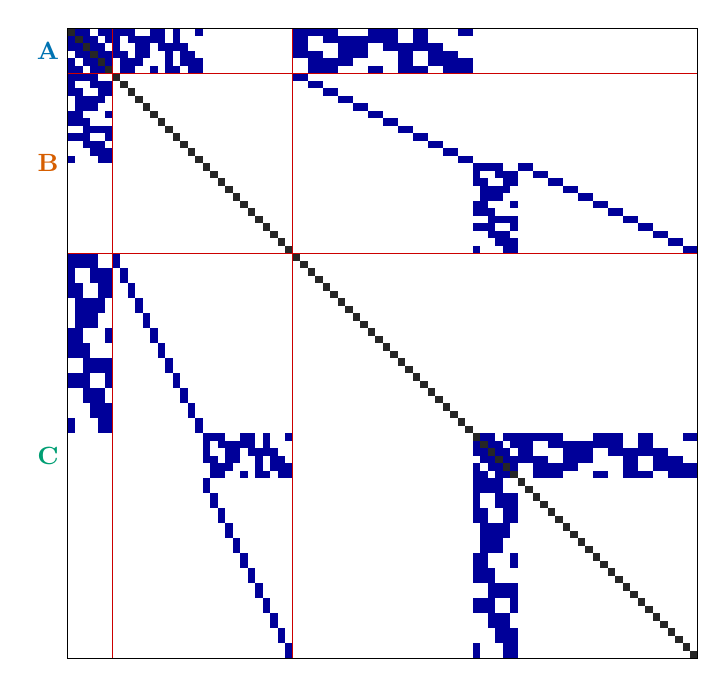
\begin{tikzpicture}[scale=1.0]
  \fill[black!85] (0.000,0.000) rectangle (0.095,-0.095);
  \fill[blue!60!black] (0.095,0.000) rectangle (0.190,-0.095);
  \fill[blue!60!black] (0.190,0.000) rectangle (0.286,-0.095);
  \fill[blue!60!black] (0.381,0.000) rectangle (0.476,-0.095);
  \fill[blue!60!black] (0.476,0.000) rectangle (0.571,-0.095);
  \fill[blue!60!black] (0.571,0.000) rectangle (0.667,-0.095);
  \fill[blue!60!black] (0.667,0.000) rectangle (0.762,-0.095);
  \fill[blue!60!black] (0.762,0.000) rectangle (0.857,-0.095);
  \fill[blue!60!black] (1.048,0.000) rectangle (1.143,-0.095);
  \fill[blue!60!black] (1.143,0.000) rectangle (1.238,-0.095);
  \fill[blue!60!black] (1.333,0.000) rectangle (1.429,-0.095);
  \fill[blue!60!black] (1.619,0.000) rectangle (1.714,-0.095);
  \fill[blue!60!black] (2.857,0.000) rectangle (2.952,-0.095);
  \fill[blue!60!black] (2.952,0.000) rectangle (3.048,-0.095);
  \fill[blue!60!black] (3.048,0.000) rectangle (3.143,-0.095);
  \fill[blue!60!black] (3.143,0.000) rectangle (3.238,-0.095);
  \fill[blue!60!black] (3.238,0.000) rectangle (3.333,-0.095);
  \fill[blue!60!black] (3.333,0.000) rectangle (3.429,-0.095);
  \fill[blue!60!black] (3.810,0.000) rectangle (3.905,-0.095);
  \fill[blue!60!black] (3.905,0.000) rectangle (4.000,-0.095);
  \fill[blue!60!black] (4.000,0.000) rectangle (4.095,-0.095);
  \fill[blue!60!black] (4.095,0.000) rectangle (4.190,-0.095);
  \fill[blue!60!black] (4.381,0.000) rectangle (4.476,-0.095);
  \fill[blue!60!black] (4.476,0.000) rectangle (4.571,-0.095);
  \fill[blue!60!black] (4.952,0.000) rectangle (5.048,-0.095);
  \fill[blue!60!black] (5.048,0.000) rectangle (5.143,-0.095);
  \fill[blue!60!black] (0.000,-0.095) rectangle (0.095,-0.190);
  \fill[black!85] (0.095,-0.095) rectangle (0.190,-0.190);
  \fill[blue!60!black] (0.190,-0.095) rectangle (0.286,-0.190);
  \fill[blue!60!black] (0.286,-0.095) rectangle (0.381,-0.190);
  \fill[blue!60!black] (0.476,-0.095) rectangle (0.571,-0.190);
  \fill[blue!60!black] (0.571,-0.095) rectangle (0.667,-0.190);
  \fill[blue!60!black] (0.762,-0.095) rectangle (0.857,-0.190);
  \fill[blue!60!black] (0.857,-0.095) rectangle (0.952,-0.190);
  \fill[blue!60!black] (0.952,-0.095) rectangle (1.048,-0.190);
  \fill[blue!60!black] (1.048,-0.095) rectangle (1.143,-0.190);
  \fill[blue!60!black] (1.143,-0.095) rectangle (1.238,-0.190);
  \fill[blue!60!black] (1.333,-0.095) rectangle (1.429,-0.190);
  \fill[blue!60!black] (2.857,-0.095) rectangle (2.952,-0.190);
  \fill[blue!60!black] (2.952,-0.095) rectangle (3.048,-0.190);
  \fill[blue!60!black] (3.238,-0.095) rectangle (3.333,-0.190);
  \fill[blue!60!black] (3.333,-0.095) rectangle (3.429,-0.190);
  \fill[blue!60!black] (3.429,-0.095) rectangle (3.524,-0.190);
  \fill[blue!60!black] (3.524,-0.095) rectangle (3.619,-0.190);
  \fill[blue!60!black] (3.619,-0.095) rectangle (3.714,-0.190);
  \fill[blue!60!black] (3.714,-0.095) rectangle (3.810,-0.190);
  \fill[blue!60!black] (3.810,-0.095) rectangle (3.905,-0.190);
  \fill[blue!60!black] (3.905,-0.095) rectangle (4.000,-0.190);
  \fill[blue!60!black] (4.000,-0.095) rectangle (4.095,-0.190);
  \fill[blue!60!black] (4.095,-0.095) rectangle (4.190,-0.190);
  \fill[blue!60!black] (4.381,-0.095) rectangle (4.476,-0.190);
  \fill[blue!60!black] (4.476,-0.095) rectangle (4.571,-0.190);
  \fill[blue!60!black] (0.000,-0.190) rectangle (0.095,-0.286);
  \fill[blue!60!black] (0.095,-0.190) rectangle (0.190,-0.286);
  \fill[black!85] (0.190,-0.190) rectangle (0.286,-0.286);
  \fill[blue!60!black] (0.286,-0.190) rectangle (0.381,-0.286);
  \fill[blue!60!black] (0.381,-0.190) rectangle (0.476,-0.286);
  \fill[blue!60!black] (0.571,-0.190) rectangle (0.667,-0.286);
  \fill[blue!60!black] (0.857,-0.190) rectangle (0.952,-0.286);
  \fill[blue!60!black] (0.952,-0.190) rectangle (1.048,-0.286);
  \fill[blue!60!black] (1.143,-0.190) rectangle (1.238,-0.286);
  \fill[blue!60!black] (1.238,-0.190) rectangle (1.333,-0.286);
  \fill[blue!60!black] (1.333,-0.190) rectangle (1.429,-0.286);
  \fill[blue!60!black] (1.429,-0.190) rectangle (1.524,-0.286);
  \fill[blue!60!black] (2.857,-0.190) rectangle (2.952,-0.286);
  \fill[blue!60!black] (2.952,-0.190) rectangle (3.048,-0.286);
  \fill[blue!60!black] (3.429,-0.190) rectangle (3.524,-0.286);
  \fill[blue!60!black] (3.524,-0.190) rectangle (3.619,-0.286);
  \fill[blue!60!black] (3.619,-0.190) rectangle (3.714,-0.286);
  \fill[blue!60!black] (3.714,-0.190) rectangle (3.810,-0.286);
  \fill[blue!60!black] (4.000,-0.190) rectangle (4.095,-0.286);
  \fill[blue!60!black] (4.095,-0.190) rectangle (4.190,-0.286);
  \fill[blue!60!black] (4.190,-0.190) rectangle (4.286,-0.286);
  \fill[blue!60!black] (4.286,-0.190) rectangle (4.381,-0.286);
  \fill[blue!60!black] (4.381,-0.190) rectangle (4.476,-0.286);
  \fill[blue!60!black] (4.476,-0.190) rectangle (4.571,-0.286);
  \fill[blue!60!black] (4.571,-0.190) rectangle (4.667,-0.286);
  \fill[blue!60!black] (4.667,-0.190) rectangle (4.762,-0.286);
  \fill[blue!60!black] (0.095,-0.286) rectangle (0.190,-0.381);
  \fill[blue!60!black] (0.190,-0.286) rectangle (0.286,-0.381);
  \fill[black!85] (0.286,-0.286) rectangle (0.381,-0.381);
  \fill[blue!60!black] (0.381,-0.286) rectangle (0.476,-0.381);
  \fill[blue!60!black] (0.476,-0.286) rectangle (0.571,-0.381);
  \fill[blue!60!black] (0.571,-0.286) rectangle (0.667,-0.381);
  \fill[blue!60!black] (0.667,-0.286) rectangle (0.762,-0.381);
  \fill[blue!60!black] (0.857,-0.286) rectangle (0.952,-0.381);
  \fill[blue!60!black] (0.952,-0.286) rectangle (1.048,-0.381);
  \fill[blue!60!black] (1.238,-0.286) rectangle (1.333,-0.381);
  \fill[blue!60!black] (1.429,-0.286) rectangle (1.524,-0.381);
  \fill[blue!60!black] (1.524,-0.286) rectangle (1.619,-0.381);
  \fill[blue!60!black] (2.857,-0.286) rectangle (2.952,-0.381);
  \fill[blue!60!black] (2.952,-0.286) rectangle (3.048,-0.381);
  \fill[blue!60!black] (3.048,-0.286) rectangle (3.143,-0.381);
  \fill[blue!60!black] (3.143,-0.286) rectangle (3.238,-0.381);
  \fill[blue!60!black] (3.429,-0.286) rectangle (3.524,-0.381);
  \fill[blue!60!black] (3.524,-0.286) rectangle (3.619,-0.381);
  \fill[blue!60!black] (3.619,-0.286) rectangle (3.714,-0.381);
  \fill[blue!60!black] (3.714,-0.286) rectangle (3.810,-0.381);
  \fill[blue!60!black] (4.190,-0.286) rectangle (4.286,-0.381);
  \fill[blue!60!black] (4.286,-0.286) rectangle (4.381,-0.381);
  \fill[blue!60!black] (4.571,-0.286) rectangle (4.667,-0.381);
  \fill[blue!60!black] (4.667,-0.286) rectangle (4.762,-0.381);
  \fill[blue!60!black] (4.762,-0.286) rectangle (4.857,-0.381);
  \fill[blue!60!black] (4.857,-0.286) rectangle (4.952,-0.381);
  \fill[blue!60!black] (0.000,-0.381) rectangle (0.095,-0.476);
  \fill[blue!60!black] (0.190,-0.381) rectangle (0.286,-0.476);
  \fill[blue!60!black] (0.286,-0.381) rectangle (0.381,-0.476);
  \fill[black!85] (0.381,-0.381) rectangle (0.476,-0.476);
  \fill[blue!60!black] (0.476,-0.381) rectangle (0.571,-0.476);
  \fill[blue!60!black] (0.667,-0.381) rectangle (0.762,-0.476);
  \fill[blue!60!black] (0.762,-0.381) rectangle (0.857,-0.476);
  \fill[blue!60!black] (0.857,-0.381) rectangle (0.952,-0.476);
  \fill[blue!60!black] (1.238,-0.381) rectangle (1.333,-0.476);
  \fill[blue!60!black] (1.429,-0.381) rectangle (1.524,-0.476);
  \fill[blue!60!black] (1.524,-0.381) rectangle (1.619,-0.476);
  \fill[blue!60!black] (1.619,-0.381) rectangle (1.714,-0.476);
  \fill[blue!60!black] (3.048,-0.381) rectangle (3.143,-0.476);
  \fill[blue!60!black] (3.143,-0.381) rectangle (3.238,-0.476);
  \fill[blue!60!black] (3.238,-0.381) rectangle (3.333,-0.476);
  \fill[blue!60!black] (3.333,-0.381) rectangle (3.429,-0.476);
  \fill[blue!60!black] (3.429,-0.381) rectangle (3.524,-0.476);
  \fill[blue!60!black] (3.524,-0.381) rectangle (3.619,-0.476);
  \fill[blue!60!black] (4.190,-0.381) rectangle (4.286,-0.476);
  \fill[blue!60!black] (4.286,-0.381) rectangle (4.381,-0.476);
  \fill[blue!60!black] (4.571,-0.381) rectangle (4.667,-0.476);
  \fill[blue!60!black] (4.667,-0.381) rectangle (4.762,-0.476);
  \fill[blue!60!black] (4.762,-0.381) rectangle (4.857,-0.476);
  \fill[blue!60!black] (4.857,-0.381) rectangle (4.952,-0.476);
  \fill[blue!60!black] (4.952,-0.381) rectangle (5.048,-0.476);
  \fill[blue!60!black] (5.048,-0.381) rectangle (5.143,-0.476);
  \fill[blue!60!black] (0.000,-0.476) rectangle (0.095,-0.571);
  \fill[blue!60!black] (0.095,-0.476) rectangle (0.190,-0.571);
  \fill[blue!60!black] (0.286,-0.476) rectangle (0.381,-0.571);
  \fill[blue!60!black] (0.381,-0.476) rectangle (0.476,-0.571);
  \fill[black!85] (0.476,-0.476) rectangle (0.571,-0.571);
  \fill[blue!60!black] (0.667,-0.476) rectangle (0.762,-0.571);
  \fill[blue!60!black] (0.762,-0.476) rectangle (0.857,-0.571);
  \fill[blue!60!black] (1.048,-0.476) rectangle (1.143,-0.571);
  \fill[blue!60!black] (1.238,-0.476) rectangle (1.333,-0.571);
  \fill[blue!60!black] (1.333,-0.476) rectangle (1.429,-0.571);
  \fill[blue!60!black] (1.524,-0.476) rectangle (1.619,-0.571);
  \fill[blue!60!black] (1.619,-0.476) rectangle (1.714,-0.571);
  \fill[blue!60!black] (3.048,-0.476) rectangle (3.143,-0.571);
  \fill[blue!60!black] (3.143,-0.476) rectangle (3.238,-0.571);
  \fill[blue!60!black] (3.238,-0.476) rectangle (3.333,-0.571);
  \fill[blue!60!black] (3.333,-0.476) rectangle (3.429,-0.571);
  \fill[blue!60!black] (3.810,-0.476) rectangle (3.905,-0.571);
  \fill[blue!60!black] (3.905,-0.476) rectangle (4.000,-0.571);
  \fill[blue!60!black] (4.190,-0.476) rectangle (4.286,-0.571);
  \fill[blue!60!black] (4.286,-0.476) rectangle (4.381,-0.571);
  \fill[blue!60!black] (4.381,-0.476) rectangle (4.476,-0.571);
  \fill[blue!60!black] (4.476,-0.476) rectangle (4.571,-0.571);
  \fill[blue!60!black] (4.762,-0.476) rectangle (4.857,-0.571);
  \fill[blue!60!black] (4.857,-0.476) rectangle (4.952,-0.571);
  \fill[blue!60!black] (4.952,-0.476) rectangle (5.048,-0.571);
  \fill[blue!60!black] (5.048,-0.476) rectangle (5.143,-0.571);
  \fill[blue!60!black] (0.000,-0.571) rectangle (0.095,-0.667);
  \fill[blue!60!black] (0.095,-0.571) rectangle (0.190,-0.667);
  \fill[blue!60!black] (0.190,-0.571) rectangle (0.286,-0.667);
  \fill[blue!60!black] (0.286,-0.571) rectangle (0.381,-0.667);
  \fill[black!85] (0.571,-0.571) rectangle (0.667,-0.667);
  \fill[blue!60!black] (2.857,-0.571) rectangle (2.952,-0.667);
  \fill[blue!60!black] (2.952,-0.571) rectangle (3.048,-0.667);
  \fill[blue!60!black] (0.000,-0.667) rectangle (0.095,-0.762);
  \fill[blue!60!black] (0.286,-0.667) rectangle (0.381,-0.762);
  \fill[blue!60!black] (0.381,-0.667) rectangle (0.476,-0.762);
  \fill[blue!60!black] (0.476,-0.667) rectangle (0.571,-0.762);
  \fill[black!85] (0.667,-0.667) rectangle (0.762,-0.762);
  \fill[blue!60!black] (3.048,-0.667) rectangle (3.143,-0.762);
  \fill[blue!60!black] (3.143,-0.667) rectangle (3.238,-0.762);
  \fill[blue!60!black] (0.000,-0.762) rectangle (0.095,-0.857);
  \fill[blue!60!black] (0.095,-0.762) rectangle (0.190,-0.857);
  \fill[blue!60!black] (0.381,-0.762) rectangle (0.476,-0.857);
  \fill[blue!60!black] (0.476,-0.762) rectangle (0.571,-0.857);
  \fill[black!85] (0.762,-0.762) rectangle (0.857,-0.857);
  \fill[blue!60!black] (3.238,-0.762) rectangle (3.333,-0.857);
  \fill[blue!60!black] (3.333,-0.762) rectangle (3.429,-0.857);
  \fill[blue!60!black] (0.095,-0.857) rectangle (0.190,-0.952);
  \fill[blue!60!black] (0.190,-0.857) rectangle (0.286,-0.952);
  \fill[blue!60!black] (0.286,-0.857) rectangle (0.381,-0.952);
  \fill[blue!60!black] (0.381,-0.857) rectangle (0.476,-0.952);
  \fill[black!85] (0.857,-0.857) rectangle (0.952,-0.952);
  \fill[blue!60!black] (3.429,-0.857) rectangle (3.524,-0.952);
  \fill[blue!60!black] (3.524,-0.857) rectangle (3.619,-0.952);
  \fill[blue!60!black] (0.095,-0.952) rectangle (0.190,-1.048);
  \fill[blue!60!black] (0.190,-0.952) rectangle (0.286,-1.048);
  \fill[blue!60!black] (0.286,-0.952) rectangle (0.381,-1.048);
  \fill[black!85] (0.952,-0.952) rectangle (1.048,-1.048);
  \fill[blue!60!black] (3.619,-0.952) rectangle (3.714,-1.048);
  \fill[blue!60!black] (3.714,-0.952) rectangle (3.810,-1.048);
  \fill[blue!60!black] (0.000,-1.048) rectangle (0.095,-1.143);
  \fill[blue!60!black] (0.095,-1.048) rectangle (0.190,-1.143);
  \fill[blue!60!black] (0.476,-1.048) rectangle (0.571,-1.143);
  \fill[black!85] (1.048,-1.048) rectangle (1.143,-1.143);
  \fill[blue!60!black] (3.810,-1.048) rectangle (3.905,-1.143);
  \fill[blue!60!black] (3.905,-1.048) rectangle (4.000,-1.143);
  \fill[blue!60!black] (0.000,-1.143) rectangle (0.095,-1.238);
  \fill[blue!60!black] (0.095,-1.143) rectangle (0.190,-1.238);
  \fill[blue!60!black] (0.190,-1.143) rectangle (0.286,-1.238);
  \fill[black!85] (1.143,-1.143) rectangle (1.238,-1.238);
  \fill[blue!60!black] (4.000,-1.143) rectangle (4.095,-1.238);
  \fill[blue!60!black] (4.095,-1.143) rectangle (4.190,-1.238);
  \fill[blue!60!black] (0.190,-1.238) rectangle (0.286,-1.333);
  \fill[blue!60!black] (0.286,-1.238) rectangle (0.381,-1.333);
  \fill[blue!60!black] (0.381,-1.238) rectangle (0.476,-1.333);
  \fill[blue!60!black] (0.476,-1.238) rectangle (0.571,-1.333);
  \fill[black!85] (1.238,-1.238) rectangle (1.333,-1.333);
  \fill[blue!60!black] (4.190,-1.238) rectangle (4.286,-1.333);
  \fill[blue!60!black] (4.286,-1.238) rectangle (4.381,-1.333);
  \fill[blue!60!black] (0.000,-1.333) rectangle (0.095,-1.429);
  \fill[blue!60!black] (0.095,-1.333) rectangle (0.190,-1.429);
  \fill[blue!60!black] (0.190,-1.333) rectangle (0.286,-1.429);
  \fill[blue!60!black] (0.476,-1.333) rectangle (0.571,-1.429);
  \fill[black!85] (1.333,-1.333) rectangle (1.429,-1.429);
  \fill[blue!60!black] (4.381,-1.333) rectangle (4.476,-1.429);
  \fill[blue!60!black] (4.476,-1.333) rectangle (4.571,-1.429);
  \fill[blue!60!black] (0.190,-1.429) rectangle (0.286,-1.524);
  \fill[blue!60!black] (0.286,-1.429) rectangle (0.381,-1.524);
  \fill[blue!60!black] (0.381,-1.429) rectangle (0.476,-1.524);
  \fill[black!85] (1.429,-1.429) rectangle (1.524,-1.524);
  \fill[blue!60!black] (4.571,-1.429) rectangle (4.667,-1.524);
  \fill[blue!60!black] (4.667,-1.429) rectangle (4.762,-1.524);
  \fill[blue!60!black] (0.286,-1.524) rectangle (0.381,-1.619);
  \fill[blue!60!black] (0.381,-1.524) rectangle (0.476,-1.619);
  \fill[blue!60!black] (0.476,-1.524) rectangle (0.571,-1.619);
  \fill[black!85] (1.524,-1.524) rectangle (1.619,-1.619);
  \fill[blue!60!black] (4.762,-1.524) rectangle (4.857,-1.619);
  \fill[blue!60!black] (4.857,-1.524) rectangle (4.952,-1.619);
  \fill[blue!60!black] (0.000,-1.619) rectangle (0.095,-1.714);
  \fill[blue!60!black] (0.381,-1.619) rectangle (0.476,-1.714);
  \fill[blue!60!black] (0.476,-1.619) rectangle (0.571,-1.714);
  \fill[black!85] (1.619,-1.619) rectangle (1.714,-1.714);
  \fill[blue!60!black] (4.952,-1.619) rectangle (5.048,-1.714);
  \fill[blue!60!black] (5.048,-1.619) rectangle (5.143,-1.714);
  \fill[black!85] (1.714,-1.714) rectangle (1.810,-1.810);
  \fill[blue!60!black] (5.143,-1.714) rectangle (5.238,-1.810);
  \fill[blue!60!black] (5.238,-1.714) rectangle (5.333,-1.810);
  \fill[blue!60!black] (5.333,-1.714) rectangle (5.429,-1.810);
  \fill[blue!60!black] (5.429,-1.714) rectangle (5.524,-1.810);
  \fill[blue!60!black] (5.714,-1.714) rectangle (5.810,-1.810);
  \fill[blue!60!black] (5.810,-1.714) rectangle (5.905,-1.810);
  \fill[black!85] (1.810,-1.810) rectangle (1.905,-1.905);
  \fill[blue!60!black] (5.143,-1.810) rectangle (5.238,-1.905);
  \fill[blue!60!black] (5.429,-1.810) rectangle (5.524,-1.905);
  \fill[blue!60!black] (5.524,-1.810) rectangle (5.619,-1.905);
  \fill[blue!60!black] (5.619,-1.810) rectangle (5.714,-1.905);
  \fill[blue!60!black] (5.905,-1.810) rectangle (6.000,-1.905);
  \fill[blue!60!black] (6.000,-1.810) rectangle (6.095,-1.905);
  \fill[black!85] (1.905,-1.905) rectangle (2.000,-2.000);
  \fill[blue!60!black] (5.143,-1.905) rectangle (5.238,-2.000);
  \fill[blue!60!black] (5.238,-1.905) rectangle (5.333,-2.000);
  \fill[blue!60!black] (5.524,-1.905) rectangle (5.619,-2.000);
  \fill[blue!60!black] (5.619,-1.905) rectangle (5.714,-2.000);
  \fill[blue!60!black] (6.095,-1.905) rectangle (6.190,-2.000);
  \fill[blue!60!black] (6.190,-1.905) rectangle (6.286,-2.000);
  \fill[black!85] (2.000,-2.000) rectangle (2.095,-2.095);
  \fill[blue!60!black] (5.238,-2.000) rectangle (5.333,-2.095);
  \fill[blue!60!black] (5.333,-2.000) rectangle (5.429,-2.095);
  \fill[blue!60!black] (5.429,-2.000) rectangle (5.524,-2.095);
  \fill[blue!60!black] (5.524,-2.000) rectangle (5.619,-2.095);
  \fill[blue!60!black] (6.286,-2.000) rectangle (6.381,-2.095);
  \fill[blue!60!black] (6.381,-2.000) rectangle (6.476,-2.095);
  \fill[black!85] (2.095,-2.095) rectangle (2.190,-2.190);
  \fill[blue!60!black] (5.238,-2.095) rectangle (5.333,-2.190);
  \fill[blue!60!black] (5.333,-2.095) rectangle (5.429,-2.190);
  \fill[blue!60!black] (5.429,-2.095) rectangle (5.524,-2.190);
  \fill[blue!60!black] (6.476,-2.095) rectangle (6.571,-2.190);
  \fill[blue!60!black] (6.571,-2.095) rectangle (6.667,-2.190);
  \fill[black!85] (2.190,-2.190) rectangle (2.286,-2.286);
  \fill[blue!60!black] (5.143,-2.190) rectangle (5.238,-2.286);
  \fill[blue!60!black] (5.238,-2.190) rectangle (5.333,-2.286);
  \fill[blue!60!black] (5.619,-2.190) rectangle (5.714,-2.286);
  \fill[blue!60!black] (6.667,-2.190) rectangle (6.762,-2.286);
  \fill[blue!60!black] (6.762,-2.190) rectangle (6.857,-2.286);
  \fill[black!85] (2.286,-2.286) rectangle (2.381,-2.381);
  \fill[blue!60!black] (5.143,-2.286) rectangle (5.238,-2.381);
  \fill[blue!60!black] (5.238,-2.286) rectangle (5.333,-2.381);
  \fill[blue!60!black] (5.333,-2.286) rectangle (5.429,-2.381);
  \fill[blue!60!black] (6.857,-2.286) rectangle (6.952,-2.381);
  \fill[blue!60!black] (6.952,-2.286) rectangle (7.048,-2.381);
  \fill[black!85] (2.381,-2.381) rectangle (2.476,-2.476);
  \fill[blue!60!black] (5.333,-2.381) rectangle (5.429,-2.476);
  \fill[blue!60!black] (5.429,-2.381) rectangle (5.524,-2.476);
  \fill[blue!60!black] (5.524,-2.381) rectangle (5.619,-2.476);
  \fill[blue!60!black] (5.619,-2.381) rectangle (5.714,-2.476);
  \fill[blue!60!black] (7.048,-2.381) rectangle (7.143,-2.476);
  \fill[blue!60!black] (7.143,-2.381) rectangle (7.238,-2.476);
  \fill[black!85] (2.476,-2.476) rectangle (2.571,-2.571);
  \fill[blue!60!black] (5.143,-2.476) rectangle (5.238,-2.571);
  \fill[blue!60!black] (5.238,-2.476) rectangle (5.333,-2.571);
  \fill[blue!60!black] (5.333,-2.476) rectangle (5.429,-2.571);
  \fill[blue!60!black] (5.619,-2.476) rectangle (5.714,-2.571);
  \fill[blue!60!black] (7.238,-2.476) rectangle (7.333,-2.571);
  \fill[blue!60!black] (7.333,-2.476) rectangle (7.429,-2.571);
  \fill[black!85] (2.571,-2.571) rectangle (2.667,-2.667);
  \fill[blue!60!black] (5.333,-2.571) rectangle (5.429,-2.667);
  \fill[blue!60!black] (5.429,-2.571) rectangle (5.524,-2.667);
  \fill[blue!60!black] (5.524,-2.571) rectangle (5.619,-2.667);
  \fill[blue!60!black] (7.429,-2.571) rectangle (7.524,-2.667);
  \fill[blue!60!black] (7.524,-2.571) rectangle (7.619,-2.667);
  \fill[black!85] (2.667,-2.667) rectangle (2.762,-2.762);
  \fill[blue!60!black] (5.429,-2.667) rectangle (5.524,-2.762);
  \fill[blue!60!black] (5.524,-2.667) rectangle (5.619,-2.762);
  \fill[blue!60!black] (5.619,-2.667) rectangle (5.714,-2.762);
  \fill[blue!60!black] (7.619,-2.667) rectangle (7.714,-2.762);
  \fill[blue!60!black] (7.714,-2.667) rectangle (7.810,-2.762);
  \fill[black!85] (2.762,-2.762) rectangle (2.857,-2.857);
  \fill[blue!60!black] (5.143,-2.762) rectangle (5.238,-2.857);
  \fill[blue!60!black] (5.524,-2.762) rectangle (5.619,-2.857);
  \fill[blue!60!black] (5.619,-2.762) rectangle (5.714,-2.857);
  \fill[blue!60!black] (7.810,-2.762) rectangle (7.905,-2.857);
  \fill[blue!60!black] (7.905,-2.762) rectangle (8.000,-2.857);
  \fill[blue!60!black] (0.000,-2.857) rectangle (0.095,-2.952);
  \fill[blue!60!black] (0.095,-2.857) rectangle (0.190,-2.952);
  \fill[blue!60!black] (0.190,-2.857) rectangle (0.286,-2.952);
  \fill[blue!60!black] (0.286,-2.857) rectangle (0.381,-2.952);
  \fill[blue!60!black] (0.571,-2.857) rectangle (0.667,-2.952);
  \fill[black!85] (2.857,-2.857) rectangle (2.952,-2.952);
  \fill[blue!60!black] (0.000,-2.952) rectangle (0.095,-3.048);
  \fill[blue!60!black] (0.095,-2.952) rectangle (0.190,-3.048);
  \fill[blue!60!black] (0.190,-2.952) rectangle (0.286,-3.048);
  \fill[blue!60!black] (0.286,-2.952) rectangle (0.381,-3.048);
  \fill[blue!60!black] (0.571,-2.952) rectangle (0.667,-3.048);
  \fill[black!85] (2.952,-2.952) rectangle (3.048,-3.048);
  \fill[blue!60!black] (0.000,-3.048) rectangle (0.095,-3.143);
  \fill[blue!60!black] (0.286,-3.048) rectangle (0.381,-3.143);
  \fill[blue!60!black] (0.381,-3.048) rectangle (0.476,-3.143);
  \fill[blue!60!black] (0.476,-3.048) rectangle (0.571,-3.143);
  \fill[blue!60!black] (0.667,-3.048) rectangle (0.762,-3.143);
  \fill[black!85] (3.048,-3.048) rectangle (3.143,-3.143);
  \fill[blue!60!black] (0.000,-3.143) rectangle (0.095,-3.238);
  \fill[blue!60!black] (0.286,-3.143) rectangle (0.381,-3.238);
  \fill[blue!60!black] (0.381,-3.143) rectangle (0.476,-3.238);
  \fill[blue!60!black] (0.476,-3.143) rectangle (0.571,-3.238);
  \fill[blue!60!black] (0.667,-3.143) rectangle (0.762,-3.238);
  \fill[black!85] (3.143,-3.143) rectangle (3.238,-3.238);
  \fill[blue!60!black] (0.000,-3.238) rectangle (0.095,-3.333);
  \fill[blue!60!black] (0.095,-3.238) rectangle (0.190,-3.333);
  \fill[blue!60!black] (0.381,-3.238) rectangle (0.476,-3.333);
  \fill[blue!60!black] (0.476,-3.238) rectangle (0.571,-3.333);
  \fill[blue!60!black] (0.762,-3.238) rectangle (0.857,-3.333);
  \fill[black!85] (3.238,-3.238) rectangle (3.333,-3.333);
  \fill[blue!60!black] (0.000,-3.333) rectangle (0.095,-3.429);
  \fill[blue!60!black] (0.095,-3.333) rectangle (0.190,-3.429);
  \fill[blue!60!black] (0.381,-3.333) rectangle (0.476,-3.429);
  \fill[blue!60!black] (0.476,-3.333) rectangle (0.571,-3.429);
  \fill[blue!60!black] (0.762,-3.333) rectangle (0.857,-3.429);
  \fill[black!85] (3.333,-3.333) rectangle (3.429,-3.429);
  \fill[blue!60!black] (0.095,-3.429) rectangle (0.190,-3.524);
  \fill[blue!60!black] (0.190,-3.429) rectangle (0.286,-3.524);
  \fill[blue!60!black] (0.286,-3.429) rectangle (0.381,-3.524);
  \fill[blue!60!black] (0.381,-3.429) rectangle (0.476,-3.524);
  \fill[blue!60!black] (0.857,-3.429) rectangle (0.952,-3.524);
  \fill[black!85] (3.429,-3.429) rectangle (3.524,-3.524);
  \fill[blue!60!black] (0.095,-3.524) rectangle (0.190,-3.619);
  \fill[blue!60!black] (0.190,-3.524) rectangle (0.286,-3.619);
  \fill[blue!60!black] (0.286,-3.524) rectangle (0.381,-3.619);
  \fill[blue!60!black] (0.381,-3.524) rectangle (0.476,-3.619);
  \fill[blue!60!black] (0.857,-3.524) rectangle (0.952,-3.619);
  \fill[black!85] (3.524,-3.524) rectangle (3.619,-3.619);
  \fill[blue!60!black] (0.095,-3.619) rectangle (0.190,-3.714);
  \fill[blue!60!black] (0.190,-3.619) rectangle (0.286,-3.714);
  \fill[blue!60!black] (0.286,-3.619) rectangle (0.381,-3.714);
  \fill[blue!60!black] (0.952,-3.619) rectangle (1.048,-3.714);
  \fill[black!85] (3.619,-3.619) rectangle (3.714,-3.714);
  \fill[blue!60!black] (0.095,-3.714) rectangle (0.190,-3.810);
  \fill[blue!60!black] (0.190,-3.714) rectangle (0.286,-3.810);
  \fill[blue!60!black] (0.286,-3.714) rectangle (0.381,-3.810);
  \fill[blue!60!black] (0.952,-3.714) rectangle (1.048,-3.810);
  \fill[black!85] (3.714,-3.714) rectangle (3.810,-3.810);
  \fill[blue!60!black] (0.000,-3.810) rectangle (0.095,-3.905);
  \fill[blue!60!black] (0.095,-3.810) rectangle (0.190,-3.905);
  \fill[blue!60!black] (0.476,-3.810) rectangle (0.571,-3.905);
  \fill[blue!60!black] (1.048,-3.810) rectangle (1.143,-3.905);
  \fill[black!85] (3.810,-3.810) rectangle (3.905,-3.905);
  \fill[blue!60!black] (0.000,-3.905) rectangle (0.095,-4.000);
  \fill[blue!60!black] (0.095,-3.905) rectangle (0.190,-4.000);
  \fill[blue!60!black] (0.476,-3.905) rectangle (0.571,-4.000);
  \fill[blue!60!black] (1.048,-3.905) rectangle (1.143,-4.000);
  \fill[black!85] (3.905,-3.905) rectangle (4.000,-4.000);
  \fill[blue!60!black] (0.000,-4.000) rectangle (0.095,-4.095);
  \fill[blue!60!black] (0.095,-4.000) rectangle (0.190,-4.095);
  \fill[blue!60!black] (0.190,-4.000) rectangle (0.286,-4.095);
  \fill[blue!60!black] (1.143,-4.000) rectangle (1.238,-4.095);
  \fill[black!85] (4.000,-4.000) rectangle (4.095,-4.095);
  \fill[blue!60!black] (0.000,-4.095) rectangle (0.095,-4.190);
  \fill[blue!60!black] (0.095,-4.095) rectangle (0.190,-4.190);
  \fill[blue!60!black] (0.190,-4.095) rectangle (0.286,-4.190);
  \fill[blue!60!black] (1.143,-4.095) rectangle (1.238,-4.190);
  \fill[black!85] (4.095,-4.095) rectangle (4.190,-4.190);
  \fill[blue!60!black] (0.190,-4.190) rectangle (0.286,-4.286);
  \fill[blue!60!black] (0.286,-4.190) rectangle (0.381,-4.286);
  \fill[blue!60!black] (0.381,-4.190) rectangle (0.476,-4.286);
  \fill[blue!60!black] (0.476,-4.190) rectangle (0.571,-4.286);
  \fill[blue!60!black] (1.238,-4.190) rectangle (1.333,-4.286);
  \fill[black!85] (4.190,-4.190) rectangle (4.286,-4.286);
  \fill[blue!60!black] (0.190,-4.286) rectangle (0.286,-4.381);
  \fill[blue!60!black] (0.286,-4.286) rectangle (0.381,-4.381);
  \fill[blue!60!black] (0.381,-4.286) rectangle (0.476,-4.381);
  \fill[blue!60!black] (0.476,-4.286) rectangle (0.571,-4.381);
  \fill[blue!60!black] (1.238,-4.286) rectangle (1.333,-4.381);
  \fill[black!85] (4.286,-4.286) rectangle (4.381,-4.381);
  \fill[blue!60!black] (0.000,-4.381) rectangle (0.095,-4.476);
  \fill[blue!60!black] (0.095,-4.381) rectangle (0.190,-4.476);
  \fill[blue!60!black] (0.190,-4.381) rectangle (0.286,-4.476);
  \fill[blue!60!black] (0.476,-4.381) rectangle (0.571,-4.476);
  \fill[blue!60!black] (1.333,-4.381) rectangle (1.429,-4.476);
  \fill[black!85] (4.381,-4.381) rectangle (4.476,-4.476);
  \fill[blue!60!black] (0.000,-4.476) rectangle (0.095,-4.571);
  \fill[blue!60!black] (0.095,-4.476) rectangle (0.190,-4.571);
  \fill[blue!60!black] (0.190,-4.476) rectangle (0.286,-4.571);
  \fill[blue!60!black] (0.476,-4.476) rectangle (0.571,-4.571);
  \fill[blue!60!black] (1.333,-4.476) rectangle (1.429,-4.571);
  \fill[black!85] (4.476,-4.476) rectangle (4.571,-4.571);
  \fill[blue!60!black] (0.190,-4.571) rectangle (0.286,-4.667);
  \fill[blue!60!black] (0.286,-4.571) rectangle (0.381,-4.667);
  \fill[blue!60!black] (0.381,-4.571) rectangle (0.476,-4.667);
  \fill[blue!60!black] (1.429,-4.571) rectangle (1.524,-4.667);
  \fill[black!85] (4.571,-4.571) rectangle (4.667,-4.667);
  \fill[blue!60!black] (0.190,-4.667) rectangle (0.286,-4.762);
  \fill[blue!60!black] (0.286,-4.667) rectangle (0.381,-4.762);
  \fill[blue!60!black] (0.381,-4.667) rectangle (0.476,-4.762);
  \fill[blue!60!black] (1.429,-4.667) rectangle (1.524,-4.762);
  \fill[black!85] (4.667,-4.667) rectangle (4.762,-4.762);
  \fill[blue!60!black] (0.286,-4.762) rectangle (0.381,-4.857);
  \fill[blue!60!black] (0.381,-4.762) rectangle (0.476,-4.857);
  \fill[blue!60!black] (0.476,-4.762) rectangle (0.571,-4.857);
  \fill[blue!60!black] (1.524,-4.762) rectangle (1.619,-4.857);
  \fill[black!85] (4.762,-4.762) rectangle (4.857,-4.857);
  \fill[blue!60!black] (0.286,-4.857) rectangle (0.381,-4.952);
  \fill[blue!60!black] (0.381,-4.857) rectangle (0.476,-4.952);
  \fill[blue!60!black] (0.476,-4.857) rectangle (0.571,-4.952);
  \fill[blue!60!black] (1.524,-4.857) rectangle (1.619,-4.952);
  \fill[black!85] (4.857,-4.857) rectangle (4.952,-4.952);
  \fill[blue!60!black] (0.000,-4.952) rectangle (0.095,-5.048);
  \fill[blue!60!black] (0.381,-4.952) rectangle (0.476,-5.048);
  \fill[blue!60!black] (0.476,-4.952) rectangle (0.571,-5.048);
  \fill[blue!60!black] (1.619,-4.952) rectangle (1.714,-5.048);
  \fill[black!85] (4.952,-4.952) rectangle (5.048,-5.048);
  \fill[blue!60!black] (0.000,-5.048) rectangle (0.095,-5.143);
  \fill[blue!60!black] (0.381,-5.048) rectangle (0.476,-5.143);
  \fill[blue!60!black] (0.476,-5.048) rectangle (0.571,-5.143);
  \fill[blue!60!black] (1.619,-5.048) rectangle (1.714,-5.143);
  \fill[black!85] (5.048,-5.048) rectangle (5.143,-5.143);
  \fill[blue!60!black] (1.714,-5.143) rectangle (1.810,-5.238);
  \fill[blue!60!black] (1.810,-5.143) rectangle (1.905,-5.238);
  \fill[blue!60!black] (1.905,-5.143) rectangle (2.000,-5.238);
  \fill[blue!60!black] (2.190,-5.143) rectangle (2.286,-5.238);
  \fill[blue!60!black] (2.286,-5.143) rectangle (2.381,-5.238);
  \fill[blue!60!black] (2.476,-5.143) rectangle (2.571,-5.238);
  \fill[blue!60!black] (2.762,-5.143) rectangle (2.857,-5.238);
  \fill[black!85] (5.143,-5.143) rectangle (5.238,-5.238);
  \fill[blue!60!black] (5.238,-5.143) rectangle (5.333,-5.238);
  \fill[blue!60!black] (5.333,-5.143) rectangle (5.429,-5.238);
  \fill[blue!60!black] (5.524,-5.143) rectangle (5.619,-5.238);
  \fill[blue!60!black] (5.619,-5.143) rectangle (5.714,-5.238);
  \fill[blue!60!black] (5.714,-5.143) rectangle (5.810,-5.238);
  \fill[blue!60!black] (5.810,-5.143) rectangle (5.905,-5.238);
  \fill[blue!60!black] (5.905,-5.143) rectangle (6.000,-5.238);
  \fill[blue!60!black] (6.000,-5.143) rectangle (6.095,-5.238);
  \fill[blue!60!black] (6.095,-5.143) rectangle (6.190,-5.238);
  \fill[blue!60!black] (6.190,-5.143) rectangle (6.286,-5.238);
  \fill[blue!60!black] (6.667,-5.143) rectangle (6.762,-5.238);
  \fill[blue!60!black] (6.762,-5.143) rectangle (6.857,-5.238);
  \fill[blue!60!black] (6.857,-5.143) rectangle (6.952,-5.238);
  \fill[blue!60!black] (6.952,-5.143) rectangle (7.048,-5.238);
  \fill[blue!60!black] (7.238,-5.143) rectangle (7.333,-5.238);
  \fill[blue!60!black] (7.333,-5.143) rectangle (7.429,-5.238);
  \fill[blue!60!black] (7.810,-5.143) rectangle (7.905,-5.238);
  \fill[blue!60!black] (7.905,-5.143) rectangle (8.000,-5.238);
  \fill[blue!60!black] (1.714,-5.238) rectangle (1.810,-5.333);
  \fill[blue!60!black] (1.905,-5.238) rectangle (2.000,-5.333);
  \fill[blue!60!black] (2.000,-5.238) rectangle (2.095,-5.333);
  \fill[blue!60!black] (2.095,-5.238) rectangle (2.190,-5.333);
  \fill[blue!60!black] (2.190,-5.238) rectangle (2.286,-5.333);
  \fill[blue!60!black] (2.286,-5.238) rectangle (2.381,-5.333);
  \fill[blue!60!black] (2.476,-5.238) rectangle (2.571,-5.333);
  \fill[blue!60!black] (5.143,-5.238) rectangle (5.238,-5.333);
  \fill[black!85] (5.238,-5.238) rectangle (5.333,-5.333);
  \fill[blue!60!black] (5.333,-5.238) rectangle (5.429,-5.333);
  \fill[blue!60!black] (5.429,-5.238) rectangle (5.524,-5.333);
  \fill[blue!60!black] (5.619,-5.238) rectangle (5.714,-5.333);
  \fill[blue!60!black] (5.714,-5.238) rectangle (5.810,-5.333);
  \fill[blue!60!black] (5.810,-5.238) rectangle (5.905,-5.333);
  \fill[blue!60!black] (6.095,-5.238) rectangle (6.190,-5.333);
  \fill[blue!60!black] (6.190,-5.238) rectangle (6.286,-5.333);
  \fill[blue!60!black] (6.286,-5.238) rectangle (6.381,-5.333);
  \fill[blue!60!black] (6.381,-5.238) rectangle (6.476,-5.333);
  \fill[blue!60!black] (6.476,-5.238) rectangle (6.571,-5.333);
  \fill[blue!60!black] (6.571,-5.238) rectangle (6.667,-5.333);
  \fill[blue!60!black] (6.667,-5.238) rectangle (6.762,-5.333);
  \fill[blue!60!black] (6.762,-5.238) rectangle (6.857,-5.333);
  \fill[blue!60!black] (6.857,-5.238) rectangle (6.952,-5.333);
  \fill[blue!60!black] (6.952,-5.238) rectangle (7.048,-5.333);
  \fill[blue!60!black] (7.238,-5.238) rectangle (7.333,-5.333);
  \fill[blue!60!black] (7.333,-5.238) rectangle (7.429,-5.333);
  \fill[blue!60!black] (1.714,-5.333) rectangle (1.810,-5.429);
  \fill[blue!60!black] (2.000,-5.333) rectangle (2.095,-5.429);
  \fill[blue!60!black] (2.095,-5.333) rectangle (2.190,-5.429);
  \fill[blue!60!black] (2.286,-5.333) rectangle (2.381,-5.429);
  \fill[blue!60!black] (2.381,-5.333) rectangle (2.476,-5.429);
  \fill[blue!60!black] (2.476,-5.333) rectangle (2.571,-5.429);
  \fill[blue!60!black] (2.571,-5.333) rectangle (2.667,-5.429);
  \fill[blue!60!black] (5.143,-5.333) rectangle (5.238,-5.429);
  \fill[blue!60!black] (5.238,-5.333) rectangle (5.333,-5.429);
  \fill[black!85] (5.333,-5.333) rectangle (5.429,-5.429);
  \fill[blue!60!black] (5.429,-5.333) rectangle (5.524,-5.429);
  \fill[blue!60!black] (5.524,-5.333) rectangle (5.619,-5.429);
  \fill[blue!60!black] (5.714,-5.333) rectangle (5.810,-5.429);
  \fill[blue!60!black] (5.810,-5.333) rectangle (5.905,-5.429);
  \fill[blue!60!black] (6.286,-5.333) rectangle (6.381,-5.429);
  \fill[blue!60!black] (6.381,-5.333) rectangle (6.476,-5.429);
  \fill[blue!60!black] (6.476,-5.333) rectangle (6.571,-5.429);
  \fill[blue!60!black] (6.571,-5.333) rectangle (6.667,-5.429);
  \fill[blue!60!black] (6.857,-5.333) rectangle (6.952,-5.429);
  \fill[blue!60!black] (6.952,-5.333) rectangle (7.048,-5.429);
  \fill[blue!60!black] (7.048,-5.333) rectangle (7.143,-5.429);
  \fill[blue!60!black] (7.143,-5.333) rectangle (7.238,-5.429);
  \fill[blue!60!black] (7.238,-5.333) rectangle (7.333,-5.429);
  \fill[blue!60!black] (7.333,-5.333) rectangle (7.429,-5.429);
  \fill[blue!60!black] (7.429,-5.333) rectangle (7.524,-5.429);
  \fill[blue!60!black] (7.524,-5.333) rectangle (7.619,-5.429);
  \fill[blue!60!black] (1.714,-5.429) rectangle (1.810,-5.524);
  \fill[blue!60!black] (1.810,-5.429) rectangle (1.905,-5.524);
  \fill[blue!60!black] (2.000,-5.429) rectangle (2.095,-5.524);
  \fill[blue!60!black] (2.095,-5.429) rectangle (2.190,-5.524);
  \fill[blue!60!black] (2.381,-5.429) rectangle (2.476,-5.524);
  \fill[blue!60!black] (2.571,-5.429) rectangle (2.667,-5.524);
  \fill[blue!60!black] (2.667,-5.429) rectangle (2.762,-5.524);
  \fill[blue!60!black] (5.238,-5.429) rectangle (5.333,-5.524);
  \fill[blue!60!black] (5.333,-5.429) rectangle (5.429,-5.524);
  \fill[black!85] (5.429,-5.429) rectangle (5.524,-5.524);
  \fill[blue!60!black] (5.524,-5.429) rectangle (5.619,-5.524);
  \fill[blue!60!black] (5.619,-5.429) rectangle (5.714,-5.524);
  \fill[blue!60!black] (5.714,-5.429) rectangle (5.810,-5.524);
  \fill[blue!60!black] (5.810,-5.429) rectangle (5.905,-5.524);
  \fill[blue!60!black] (5.905,-5.429) rectangle (6.000,-5.524);
  \fill[blue!60!black] (6.000,-5.429) rectangle (6.095,-5.524);
  \fill[blue!60!black] (6.286,-5.429) rectangle (6.381,-5.524);
  \fill[blue!60!black] (6.381,-5.429) rectangle (6.476,-5.524);
  \fill[blue!60!black] (6.476,-5.429) rectangle (6.571,-5.524);
  \fill[blue!60!black] (6.571,-5.429) rectangle (6.667,-5.524);
  \fill[blue!60!black] (7.048,-5.429) rectangle (7.143,-5.524);
  \fill[blue!60!black] (7.143,-5.429) rectangle (7.238,-5.524);
  \fill[blue!60!black] (7.429,-5.429) rectangle (7.524,-5.524);
  \fill[blue!60!black] (7.524,-5.429) rectangle (7.619,-5.524);
  \fill[blue!60!black] (7.619,-5.429) rectangle (7.714,-5.524);
  \fill[blue!60!black] (7.714,-5.429) rectangle (7.810,-5.524);
  \fill[blue!60!black] (1.810,-5.524) rectangle (1.905,-5.619);
  \fill[blue!60!black] (1.905,-5.524) rectangle (2.000,-5.619);
  \fill[blue!60!black] (2.000,-5.524) rectangle (2.095,-5.619);
  \fill[blue!60!black] (2.381,-5.524) rectangle (2.476,-5.619);
  \fill[blue!60!black] (2.571,-5.524) rectangle (2.667,-5.619);
  \fill[blue!60!black] (2.667,-5.524) rectangle (2.762,-5.619);
  \fill[blue!60!black] (2.762,-5.524) rectangle (2.857,-5.619);
  \fill[blue!60!black] (5.143,-5.524) rectangle (5.238,-5.619);
  \fill[blue!60!black] (5.333,-5.524) rectangle (5.429,-5.619);
  \fill[blue!60!black] (5.429,-5.524) rectangle (5.524,-5.619);
  \fill[black!85] (5.524,-5.524) rectangle (5.619,-5.619);
  \fill[blue!60!black] (5.619,-5.524) rectangle (5.714,-5.619);
  \fill[blue!60!black] (5.905,-5.524) rectangle (6.000,-5.619);
  \fill[blue!60!black] (6.000,-5.524) rectangle (6.095,-5.619);
  \fill[blue!60!black] (6.095,-5.524) rectangle (6.190,-5.619);
  \fill[blue!60!black] (6.190,-5.524) rectangle (6.286,-5.619);
  \fill[blue!60!black] (6.286,-5.524) rectangle (6.381,-5.619);
  \fill[blue!60!black] (6.381,-5.524) rectangle (6.476,-5.619);
  \fill[blue!60!black] (7.048,-5.524) rectangle (7.143,-5.619);
  \fill[blue!60!black] (7.143,-5.524) rectangle (7.238,-5.619);
  \fill[blue!60!black] (7.429,-5.524) rectangle (7.524,-5.619);
  \fill[blue!60!black] (7.524,-5.524) rectangle (7.619,-5.619);
  \fill[blue!60!black] (7.619,-5.524) rectangle (7.714,-5.619);
  \fill[blue!60!black] (7.714,-5.524) rectangle (7.810,-5.619);
  \fill[blue!60!black] (7.810,-5.524) rectangle (7.905,-5.619);
  \fill[blue!60!black] (7.905,-5.524) rectangle (8.000,-5.619);
  \fill[blue!60!black] (1.810,-5.619) rectangle (1.905,-5.714);
  \fill[blue!60!black] (1.905,-5.619) rectangle (2.000,-5.714);
  \fill[blue!60!black] (2.190,-5.619) rectangle (2.286,-5.714);
  \fill[blue!60!black] (2.381,-5.619) rectangle (2.476,-5.714);
  \fill[blue!60!black] (2.476,-5.619) rectangle (2.571,-5.714);
  \fill[blue!60!black] (2.667,-5.619) rectangle (2.762,-5.714);
  \fill[blue!60!black] (2.762,-5.619) rectangle (2.857,-5.714);
  \fill[blue!60!black] (5.143,-5.619) rectangle (5.238,-5.714);
  \fill[blue!60!black] (5.238,-5.619) rectangle (5.333,-5.714);
  \fill[blue!60!black] (5.429,-5.619) rectangle (5.524,-5.714);
  \fill[blue!60!black] (5.524,-5.619) rectangle (5.619,-5.714);
  \fill[black!85] (5.619,-5.619) rectangle (5.714,-5.714);
  \fill[blue!60!black] (5.905,-5.619) rectangle (6.000,-5.714);
  \fill[blue!60!black] (6.000,-5.619) rectangle (6.095,-5.714);
  \fill[blue!60!black] (6.095,-5.619) rectangle (6.190,-5.714);
  \fill[blue!60!black] (6.190,-5.619) rectangle (6.286,-5.714);
  \fill[blue!60!black] (6.667,-5.619) rectangle (6.762,-5.714);
  \fill[blue!60!black] (6.762,-5.619) rectangle (6.857,-5.714);
  \fill[blue!60!black] (7.048,-5.619) rectangle (7.143,-5.714);
  \fill[blue!60!black] (7.143,-5.619) rectangle (7.238,-5.714);
  \fill[blue!60!black] (7.238,-5.619) rectangle (7.333,-5.714);
  \fill[blue!60!black] (7.333,-5.619) rectangle (7.429,-5.714);
  \fill[blue!60!black] (7.619,-5.619) rectangle (7.714,-5.714);
  \fill[blue!60!black] (7.714,-5.619) rectangle (7.810,-5.714);
  \fill[blue!60!black] (7.810,-5.619) rectangle (7.905,-5.714);
  \fill[blue!60!black] (7.905,-5.619) rectangle (8.000,-5.714);
  \fill[blue!60!black] (1.714,-5.714) rectangle (1.810,-5.810);
  \fill[blue!60!black] (5.143,-5.714) rectangle (5.238,-5.810);
  \fill[blue!60!black] (5.238,-5.714) rectangle (5.333,-5.810);
  \fill[blue!60!black] (5.333,-5.714) rectangle (5.429,-5.810);
  \fill[blue!60!black] (5.429,-5.714) rectangle (5.524,-5.810);
  \fill[black!85] (5.714,-5.714) rectangle (5.810,-5.810);
  \fill[blue!60!black] (1.714,-5.810) rectangle (1.810,-5.905);
  \fill[blue!60!black] (5.143,-5.810) rectangle (5.238,-5.905);
  \fill[blue!60!black] (5.238,-5.810) rectangle (5.333,-5.905);
  \fill[blue!60!black] (5.333,-5.810) rectangle (5.429,-5.905);
  \fill[blue!60!black] (5.429,-5.810) rectangle (5.524,-5.905);
  \fill[black!85] (5.810,-5.810) rectangle (5.905,-5.905);
  \fill[blue!60!black] (1.810,-5.905) rectangle (1.905,-6.000);
  \fill[blue!60!black] (5.143,-5.905) rectangle (5.238,-6.000);
  \fill[blue!60!black] (5.429,-5.905) rectangle (5.524,-6.000);
  \fill[blue!60!black] (5.524,-5.905) rectangle (5.619,-6.000);
  \fill[blue!60!black] (5.619,-5.905) rectangle (5.714,-6.000);
  \fill[black!85] (5.905,-5.905) rectangle (6.000,-6.000);
  \fill[blue!60!black] (1.810,-6.000) rectangle (1.905,-6.095);
  \fill[blue!60!black] (5.143,-6.000) rectangle (5.238,-6.095);
  \fill[blue!60!black] (5.429,-6.000) rectangle (5.524,-6.095);
  \fill[blue!60!black] (5.524,-6.000) rectangle (5.619,-6.095);
  \fill[blue!60!black] (5.619,-6.000) rectangle (5.714,-6.095);
  \fill[black!85] (6.000,-6.000) rectangle (6.095,-6.095);
  \fill[blue!60!black] (1.905,-6.095) rectangle (2.000,-6.190);
  \fill[blue!60!black] (5.143,-6.095) rectangle (5.238,-6.190);
  \fill[blue!60!black] (5.238,-6.095) rectangle (5.333,-6.190);
  \fill[blue!60!black] (5.524,-6.095) rectangle (5.619,-6.190);
  \fill[blue!60!black] (5.619,-6.095) rectangle (5.714,-6.190);
  \fill[black!85] (6.095,-6.095) rectangle (6.190,-6.190);
  \fill[blue!60!black] (1.905,-6.190) rectangle (2.000,-6.286);
  \fill[blue!60!black] (5.143,-6.190) rectangle (5.238,-6.286);
  \fill[blue!60!black] (5.238,-6.190) rectangle (5.333,-6.286);
  \fill[blue!60!black] (5.524,-6.190) rectangle (5.619,-6.286);
  \fill[blue!60!black] (5.619,-6.190) rectangle (5.714,-6.286);
  \fill[black!85] (6.190,-6.190) rectangle (6.286,-6.286);
  \fill[blue!60!black] (2.000,-6.286) rectangle (2.095,-6.381);
  \fill[blue!60!black] (5.238,-6.286) rectangle (5.333,-6.381);
  \fill[blue!60!black] (5.333,-6.286) rectangle (5.429,-6.381);
  \fill[blue!60!black] (5.429,-6.286) rectangle (5.524,-6.381);
  \fill[blue!60!black] (5.524,-6.286) rectangle (5.619,-6.381);
  \fill[black!85] (6.286,-6.286) rectangle (6.381,-6.381);
  \fill[blue!60!black] (2.000,-6.381) rectangle (2.095,-6.476);
  \fill[blue!60!black] (5.238,-6.381) rectangle (5.333,-6.476);
  \fill[blue!60!black] (5.333,-6.381) rectangle (5.429,-6.476);
  \fill[blue!60!black] (5.429,-6.381) rectangle (5.524,-6.476);
  \fill[blue!60!black] (5.524,-6.381) rectangle (5.619,-6.476);
  \fill[black!85] (6.381,-6.381) rectangle (6.476,-6.476);
  \fill[blue!60!black] (2.095,-6.476) rectangle (2.190,-6.571);
  \fill[blue!60!black] (5.238,-6.476) rectangle (5.333,-6.571);
  \fill[blue!60!black] (5.333,-6.476) rectangle (5.429,-6.571);
  \fill[blue!60!black] (5.429,-6.476) rectangle (5.524,-6.571);
  \fill[black!85] (6.476,-6.476) rectangle (6.571,-6.571);
  \fill[blue!60!black] (2.095,-6.571) rectangle (2.190,-6.667);
  \fill[blue!60!black] (5.238,-6.571) rectangle (5.333,-6.667);
  \fill[blue!60!black] (5.333,-6.571) rectangle (5.429,-6.667);
  \fill[blue!60!black] (5.429,-6.571) rectangle (5.524,-6.667);
  \fill[black!85] (6.571,-6.571) rectangle (6.667,-6.667);
  \fill[blue!60!black] (2.190,-6.667) rectangle (2.286,-6.762);
  \fill[blue!60!black] (5.143,-6.667) rectangle (5.238,-6.762);
  \fill[blue!60!black] (5.238,-6.667) rectangle (5.333,-6.762);
  \fill[blue!60!black] (5.619,-6.667) rectangle (5.714,-6.762);
  \fill[black!85] (6.667,-6.667) rectangle (6.762,-6.762);
  \fill[blue!60!black] (2.190,-6.762) rectangle (2.286,-6.857);
  \fill[blue!60!black] (5.143,-6.762) rectangle (5.238,-6.857);
  \fill[blue!60!black] (5.238,-6.762) rectangle (5.333,-6.857);
  \fill[blue!60!black] (5.619,-6.762) rectangle (5.714,-6.857);
  \fill[black!85] (6.762,-6.762) rectangle (6.857,-6.857);
  \fill[blue!60!black] (2.286,-6.857) rectangle (2.381,-6.952);
  \fill[blue!60!black] (5.143,-6.857) rectangle (5.238,-6.952);
  \fill[blue!60!black] (5.238,-6.857) rectangle (5.333,-6.952);
  \fill[blue!60!black] (5.333,-6.857) rectangle (5.429,-6.952);
  \fill[black!85] (6.857,-6.857) rectangle (6.952,-6.952);
  \fill[blue!60!black] (2.286,-6.952) rectangle (2.381,-7.048);
  \fill[blue!60!black] (5.143,-6.952) rectangle (5.238,-7.048);
  \fill[blue!60!black] (5.238,-6.952) rectangle (5.333,-7.048);
  \fill[blue!60!black] (5.333,-6.952) rectangle (5.429,-7.048);
  \fill[black!85] (6.952,-6.952) rectangle (7.048,-7.048);
  \fill[blue!60!black] (2.381,-7.048) rectangle (2.476,-7.143);
  \fill[blue!60!black] (5.333,-7.048) rectangle (5.429,-7.143);
  \fill[blue!60!black] (5.429,-7.048) rectangle (5.524,-7.143);
  \fill[blue!60!black] (5.524,-7.048) rectangle (5.619,-7.143);
  \fill[blue!60!black] (5.619,-7.048) rectangle (5.714,-7.143);
  \fill[black!85] (7.048,-7.048) rectangle (7.143,-7.143);
  \fill[blue!60!black] (2.381,-7.143) rectangle (2.476,-7.238);
  \fill[blue!60!black] (5.333,-7.143) rectangle (5.429,-7.238);
  \fill[blue!60!black] (5.429,-7.143) rectangle (5.524,-7.238);
  \fill[blue!60!black] (5.524,-7.143) rectangle (5.619,-7.238);
  \fill[blue!60!black] (5.619,-7.143) rectangle (5.714,-7.238);
  \fill[black!85] (7.143,-7.143) rectangle (7.238,-7.238);
  \fill[blue!60!black] (2.476,-7.238) rectangle (2.571,-7.333);
  \fill[blue!60!black] (5.143,-7.238) rectangle (5.238,-7.333);
  \fill[blue!60!black] (5.238,-7.238) rectangle (5.333,-7.333);
  \fill[blue!60!black] (5.333,-7.238) rectangle (5.429,-7.333);
  \fill[blue!60!black] (5.619,-7.238) rectangle (5.714,-7.333);
  \fill[black!85] (7.238,-7.238) rectangle (7.333,-7.333);
  \fill[blue!60!black] (2.476,-7.333) rectangle (2.571,-7.429);
  \fill[blue!60!black] (5.143,-7.333) rectangle (5.238,-7.429);
  \fill[blue!60!black] (5.238,-7.333) rectangle (5.333,-7.429);
  \fill[blue!60!black] (5.333,-7.333) rectangle (5.429,-7.429);
  \fill[blue!60!black] (5.619,-7.333) rectangle (5.714,-7.429);
  \fill[black!85] (7.333,-7.333) rectangle (7.429,-7.429);
  \fill[blue!60!black] (2.571,-7.429) rectangle (2.667,-7.524);
  \fill[blue!60!black] (5.333,-7.429) rectangle (5.429,-7.524);
  \fill[blue!60!black] (5.429,-7.429) rectangle (5.524,-7.524);
  \fill[blue!60!black] (5.524,-7.429) rectangle (5.619,-7.524);
  \fill[black!85] (7.429,-7.429) rectangle (7.524,-7.524);
  \fill[blue!60!black] (2.571,-7.524) rectangle (2.667,-7.619);
  \fill[blue!60!black] (5.333,-7.524) rectangle (5.429,-7.619);
  \fill[blue!60!black] (5.429,-7.524) rectangle (5.524,-7.619);
  \fill[blue!60!black] (5.524,-7.524) rectangle (5.619,-7.619);
  \fill[black!85] (7.524,-7.524) rectangle (7.619,-7.619);
  \fill[blue!60!black] (2.667,-7.619) rectangle (2.762,-7.714);
  \fill[blue!60!black] (5.429,-7.619) rectangle (5.524,-7.714);
  \fill[blue!60!black] (5.524,-7.619) rectangle (5.619,-7.714);
  \fill[blue!60!black] (5.619,-7.619) rectangle (5.714,-7.714);
  \fill[black!85] (7.619,-7.619) rectangle (7.714,-7.714);
  \fill[blue!60!black] (2.667,-7.714) rectangle (2.762,-7.810);
  \fill[blue!60!black] (5.429,-7.714) rectangle (5.524,-7.810);
  \fill[blue!60!black] (5.524,-7.714) rectangle (5.619,-7.810);
  \fill[blue!60!black] (5.619,-7.714) rectangle (5.714,-7.810);
  \fill[black!85] (7.714,-7.714) rectangle (7.810,-7.810);
  \fill[blue!60!black] (2.762,-7.810) rectangle (2.857,-7.905);
  \fill[blue!60!black] (5.143,-7.810) rectangle (5.238,-7.905);
  \fill[blue!60!black] (5.524,-7.810) rectangle (5.619,-7.905);
  \fill[blue!60!black] (5.619,-7.810) rectangle (5.714,-7.905);
  \fill[black!85] (7.810,-7.810) rectangle (7.905,-7.905);
  \fill[blue!60!black] (2.762,-7.905) rectangle (2.857,-8.000);
  \fill[blue!60!black] (5.143,-7.905) rectangle (5.238,-8.000);
  \fill[blue!60!black] (5.524,-7.905) rectangle (5.619,-8.000);
  \fill[blue!60!black] (5.619,-7.905) rectangle (5.714,-8.000);
  \fill[black!85] (7.905,-7.905) rectangle (8.000,-8.000);
  \draw[red!80!black, line width=0.4pt] (0.571,0.000) -- (0.571,-8.000);
  \draw[red!80!black, line width=0.4pt] (0,-0.571) -- (8.000,-0.571);
  \draw[red!80!black, line width=0.4pt] (2.857,0.000) -- (2.857,-8.000);
  \draw[red!80!black, line width=0.4pt] (0,-2.857) -- (8.000,-2.857);
  \draw[black, line width=0.3pt] (0,0) rectangle (8.000,-8.000);
  \definecolor{hml0}{rgb}{0.000, 0.450, 0.700}
  \node[font=\small\bfseries, hml0] at (-0.25,-0.286) {A};
  \definecolor{hml1}{rgb}{0.840, 0.370, 0.000}
  \node[font=\small\bfseries, hml1] at (-0.25,-1.714) {B};
  \definecolor{hml2}{rgb}{0.000, 0.620, 0.450}
  \node[font=\small\bfseries, hml2] at (-0.25,-5.429) {C};
\end{tikzpicture}
  \caption{Adjacency heatmap (rows/columns sorted by tier): the binary co-occurrence shadow of the ternary structure above; included as a tier-block-structure diagnostic.}
\end{subfigure}
\caption{$Q_{84}$: $\Ccls$-closure of the Adjacent ternary graph on $6$ vertices ($36$ edges).}
\label{fig:q84}
\end{figure}
% Auto-generated by paper/scripts/dump_quotient_to_tikz.py
% Do not hand-edit; regenerate via `python3 dump_quotient_to_tikz.py`.
\begin{figure}[H]
\centering
\begin{subfigure}[t]{\textwidth}
  \centering
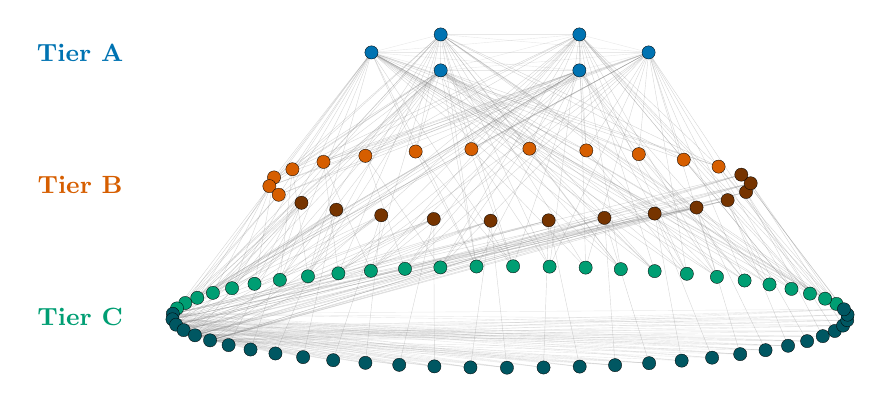
\begin{tikzpicture}[scale=1.4]
  \draw[gray, line width=0.15pt, opacity=0.18] (1.257,1.200) -- (0.629,1.363);
  \draw[gray, line width=0.15pt, opacity=0.18] (1.257,1.200) -- (-0.629,1.363);
  \draw[gray, line width=0.15pt, opacity=0.18] (1.257,1.200) -- (-1.257,1.200);
  \draw[gray, line width=0.15pt, opacity=0.18] (1.257,1.200) -- (-0.629,1.037);
  \draw[gray, line width=0.15pt, opacity=0.18] (1.257,1.200) -- (0.629,1.037);
  \draw[gray, line width=0.15pt, opacity=0.32] (1.257,1.200) -- (1.576,0.227);
  \draw[gray, line width=0.15pt, opacity=0.32] (1.257,1.200) -- (1.168,0.277);
  \draw[gray, line width=0.15pt, opacity=0.32] (1.257,1.200) -- (0.692,0.311);
  \draw[gray, line width=0.15pt, opacity=0.32] (1.257,1.200) -- (-0.350,0.323);
  \draw[gray, line width=0.15pt, opacity=0.32] (1.257,1.200) -- (-1.312,0.262);
  \draw[gray, line width=0.15pt, opacity=0.32] (1.257,1.200) -- (-1.692,0.207);
  \draw[gray, line width=0.15pt, opacity=0.32] (1.257,1.200) -- (-2.183,-0.013);
  \draw[gray, line width=0.15pt, opacity=0.32] (1.257,1.200) -- (-2.098,-0.091);
  \draw[gray, line width=0.15pt, opacity=0.32] (1.257,1.200) -- (2.721,-0.988);
  \draw[gray, line width=0.15pt, opacity=0.32] (1.257,1.200) -- (2.553,-0.945);
  \draw[gray, line width=0.15pt, opacity=0.32] (1.257,1.200) -- (2.354,-0.905);
  \draw[gray, line width=0.15pt, opacity=0.32] (1.257,1.200) -- (2.128,-0.869);
  \draw[gray, line width=0.15pt, opacity=0.32] (1.257,1.200) -- (1.877,-0.836);
  \draw[gray, line width=0.15pt, opacity=0.32] (1.257,1.200) -- (1.604,-0.808);
  \draw[gray, line width=0.15pt, opacity=0.32] (1.257,1.200) -- (0.686,-0.752);
  \draw[gray, line width=0.15pt, opacity=0.32] (1.257,1.200) -- (0.359,-0.743);
  \draw[gray, line width=0.15pt, opacity=0.32] (1.257,1.200) -- (-0.632,-0.750);
  \draw[gray, line width=0.15pt, opacity=0.32] (1.257,1.200) -- (-0.953,-0.763);
  \draw[gray, line width=0.15pt, opacity=0.32] (1.257,1.200) -- (-1.262,-0.781);
  \draw[gray, line width=0.15pt, opacity=0.32] (1.257,1.200) -- (-1.557,-0.804);
  \draw[gray, line width=0.15pt, opacity=0.32] (1.257,1.200) -- (-2.695,-0.981);
  \draw[gray, line width=0.15pt, opacity=0.32] (1.257,1.200) -- (-2.837,-1.026);
  \draw[gray, line width=0.15pt, opacity=0.32] (1.257,1.200) -- (-3.021,-1.122);
  \draw[gray, line width=0.15pt, opacity=0.18] (0.629,1.363) -- (-0.629,1.363);
  \draw[gray, line width=0.15pt, opacity=0.18] (0.629,1.363) -- (-1.257,1.200);
  \draw[gray, line width=0.15pt, opacity=0.18] (0.629,1.363) -- (-0.629,1.037);
  \draw[gray, line width=0.15pt, opacity=0.18] (0.629,1.363) -- (0.629,1.037);
  \draw[gray, line width=0.15pt, opacity=0.32] (0.629,1.363) -- (1.892,0.164);
  \draw[gray, line width=0.15pt, opacity=0.32] (0.629,1.363) -- (1.576,0.227);
  \draw[gray, line width=0.15pt, opacity=0.32] (0.629,1.363) -- (0.692,0.311);
  \draw[gray, line width=0.15pt, opacity=0.32] (0.629,1.363) -- (0.176,0.327);
  \draw[gray, line width=0.15pt, opacity=0.32] (0.629,1.363) -- (-0.350,0.323);
  \draw[gray, line width=0.15pt, opacity=0.32] (0.629,1.363) -- (-1.312,0.262);
  \draw[gray, line width=0.15pt, opacity=0.32] (0.629,1.363) -- (-1.692,0.207);
  \draw[gray, line width=0.15pt, opacity=0.32] (0.629,1.363) -- (-1.974,0.140);
  \draw[gray, line width=0.15pt, opacity=0.32] (0.629,1.363) -- (2.961,-1.081);
  \draw[gray, line width=0.15pt, opacity=0.32] (0.629,1.363) -- (2.858,-1.034);
  \draw[gray, line width=0.15pt, opacity=0.32] (0.629,1.363) -- (2.721,-0.988);
  \draw[gray, line width=0.15pt, opacity=0.32] (0.629,1.363) -- (2.553,-0.945);
  \draw[gray, line width=0.15pt, opacity=0.32] (0.629,1.363) -- (1.877,-0.836);
  \draw[gray, line width=0.15pt, opacity=0.32] (0.629,1.363) -- (1.604,-0.808);
  \draw[gray, line width=0.15pt, opacity=0.32] (0.629,1.363) -- (1.312,-0.784);
  \draw[gray, line width=0.15pt, opacity=0.32] (0.629,1.363) -- (1.005,-0.766);
  \draw[gray, line width=0.15pt, opacity=0.32] (0.629,1.363) -- (0.686,-0.752);
  \draw[gray, line width=0.15pt, opacity=0.32] (0.629,1.363) -- (0.359,-0.743);
  \draw[gray, line width=0.15pt, opacity=0.32] (0.629,1.363) -- (-0.632,-0.750);
  \draw[gray, line width=0.15pt, opacity=0.32] (0.629,1.363) -- (-0.953,-0.763);
  \draw[gray, line width=0.15pt, opacity=0.32] (0.629,1.363) -- (-1.262,-0.781);
  \draw[gray, line width=0.15pt, opacity=0.32] (0.629,1.363) -- (-1.557,-0.804);
  \draw[gray, line width=0.15pt, opacity=0.32] (0.629,1.363) -- (-1.833,-0.831);
  \draw[gray, line width=0.15pt, opacity=0.32] (0.629,1.363) -- (-2.088,-0.863);
  \draw[gray, line width=0.15pt, opacity=0.18] (-0.629,1.363) -- (-1.257,1.200);
  \draw[gray, line width=0.15pt, opacity=0.18] (-0.629,1.363) -- (-0.629,1.037);
  \draw[gray, line width=0.15pt, opacity=0.32] (-0.629,1.363) -- (1.892,0.164);
  \draw[gray, line width=0.15pt, opacity=0.32] (-0.629,1.363) -- (1.576,0.227);
  \draw[gray, line width=0.15pt, opacity=0.32] (-0.629,1.363) -- (0.176,0.327);
  \draw[gray, line width=0.15pt, opacity=0.32] (-0.629,1.363) -- (-0.350,0.323);
  \draw[gray, line width=0.15pt, opacity=0.32] (-0.629,1.363) -- (-0.856,0.301);
  \draw[gray, line width=0.15pt, opacity=0.32] (-0.629,1.363) -- (-1.692,0.207);
  \draw[gray, line width=0.15pt, opacity=0.32] (-0.629,1.363) -- (-1.974,0.140);
  \draw[gray, line width=0.15pt, opacity=0.32] (-0.629,1.363) -- (-2.183,-0.013);
  \draw[gray, line width=0.15pt, opacity=0.32] (-0.629,1.363) -- (2.961,-1.081);
  \draw[gray, line width=0.15pt, opacity=0.32] (-0.629,1.363) -- (2.858,-1.034);
  \draw[gray, line width=0.15pt, opacity=0.32] (-0.629,1.363) -- (2.721,-0.988);
  \draw[gray, line width=0.15pt, opacity=0.32] (-0.629,1.363) -- (2.553,-0.945);
  \draw[gray, line width=0.15pt, opacity=0.32] (-0.629,1.363) -- (1.312,-0.784);
  \draw[gray, line width=0.15pt, opacity=0.32] (-0.629,1.363) -- (1.005,-0.766);
  \draw[gray, line width=0.15pt, opacity=0.32] (-0.629,1.363) -- (0.686,-0.752);
  \draw[gray, line width=0.15pt, opacity=0.32] (-0.629,1.363) -- (0.359,-0.743);
  \draw[gray, line width=0.15pt, opacity=0.32] (-0.629,1.363) -- (0.028,-0.740);
  \draw[gray, line width=0.15pt, opacity=0.32] (-0.629,1.363) -- (-0.304,-0.742);
  \draw[gray, line width=0.15pt, opacity=0.32] (-0.629,1.363) -- (-1.262,-0.781);
  \draw[gray, line width=0.15pt, opacity=0.32] (-0.629,1.363) -- (-1.557,-0.804);
  \draw[gray, line width=0.15pt, opacity=0.32] (-0.629,1.363) -- (-1.833,-0.831);
  \draw[gray, line width=0.15pt, opacity=0.32] (-0.629,1.363) -- (-2.088,-0.863);
  \draw[gray, line width=0.15pt, opacity=0.32] (-0.629,1.363) -- (-2.695,-0.981);
  \draw[gray, line width=0.15pt, opacity=0.32] (-0.629,1.363) -- (-2.837,-1.026);
  \draw[gray, line width=0.15pt, opacity=0.18] (-1.257,1.200) -- (-0.629,1.037);
  \draw[gray, line width=0.15pt, opacity=0.18] (-1.257,1.200) -- (0.629,1.037);
  \draw[gray, line width=0.15pt, opacity=0.32] (-1.257,1.200) -- (1.892,0.164);
  \draw[gray, line width=0.15pt, opacity=0.32] (-1.257,1.200) -- (1.576,0.227);
  \draw[gray, line width=0.15pt, opacity=0.32] (-1.257,1.200) -- (1.168,0.277);
  \draw[gray, line width=0.15pt, opacity=0.32] (-1.257,1.200) -- (0.692,0.311);
  \draw[gray, line width=0.15pt, opacity=0.32] (-1.257,1.200) -- (0.176,0.327);
  \draw[gray, line width=0.15pt, opacity=0.32] (-1.257,1.200) -- (-0.856,0.301);
  \draw[gray, line width=0.15pt, opacity=0.32] (-1.257,1.200) -- (-1.974,0.140);
  \draw[gray, line width=0.15pt, opacity=0.32] (-1.257,1.200) -- (-2.141,0.066);
  \draw[gray, line width=0.15pt, opacity=0.32] (-1.257,1.200) -- (-2.098,-0.091);
  \draw[gray, line width=0.15pt, opacity=0.32] (-1.257,1.200) -- (2.961,-1.081);
  \draw[gray, line width=0.15pt, opacity=0.32] (-1.257,1.200) -- (2.858,-1.034);
  \draw[gray, line width=0.15pt, opacity=0.32] (-1.257,1.200) -- (2.721,-0.988);
  \draw[gray, line width=0.15pt, opacity=0.32] (-1.257,1.200) -- (2.553,-0.945);
  \draw[gray, line width=0.15pt, opacity=0.32] (-1.257,1.200) -- (2.354,-0.905);
  \draw[gray, line width=0.15pt, opacity=0.32] (-1.257,1.200) -- (2.128,-0.869);
  \draw[gray, line width=0.15pt, opacity=0.32] (-1.257,1.200) -- (1.877,-0.836);
  \draw[gray, line width=0.15pt, opacity=0.32] (-1.257,1.200) -- (1.604,-0.808);
  \draw[gray, line width=0.15pt, opacity=0.32] (-1.257,1.200) -- (1.312,-0.784);
  \draw[gray, line width=0.15pt, opacity=0.32] (-1.257,1.200) -- (1.005,-0.766);
  \draw[gray, line width=0.15pt, opacity=0.32] (-1.257,1.200) -- (0.028,-0.740);
  \draw[gray, line width=0.15pt, opacity=0.32] (-1.257,1.200) -- (-0.304,-0.742);
  \draw[gray, line width=0.15pt, opacity=0.32] (-1.257,1.200) -- (-1.833,-0.831);
  \draw[gray, line width=0.15pt, opacity=0.32] (-1.257,1.200) -- (-2.088,-0.863);
  \draw[gray, line width=0.15pt, opacity=0.32] (-1.257,1.200) -- (-2.318,-0.899);
  \draw[gray, line width=0.15pt, opacity=0.32] (-1.257,1.200) -- (-2.522,-0.939);
  \draw[gray, line width=0.15pt, opacity=0.32] (-1.257,1.200) -- (-2.946,-1.073);
  \draw[gray, line width=0.15pt, opacity=0.32] (-1.257,1.200) -- (-3.021,-1.122);
  \draw[gray, line width=0.15pt, opacity=0.18] (-0.629,1.037) -- (0.629,1.037);
  \draw[gray, line width=0.15pt, opacity=0.32] (-0.629,1.037) -- (1.892,0.164);
  \draw[gray, line width=0.15pt, opacity=0.32] (-0.629,1.037) -- (1.168,0.277);
  \draw[gray, line width=0.15pt, opacity=0.32] (-0.629,1.037) -- (0.692,0.311);
  \draw[gray, line width=0.15pt, opacity=0.32] (-0.629,1.037) -- (0.176,0.327);
  \draw[gray, line width=0.15pt, opacity=0.32] (-0.629,1.037) -- (-0.856,0.301);
  \draw[gray, line width=0.15pt, opacity=0.32] (-0.629,1.037) -- (-1.974,0.140);
  \draw[gray, line width=0.15pt, opacity=0.32] (-0.629,1.037) -- (-2.141,0.066);
  \draw[gray, line width=0.15pt, opacity=0.32] (-0.629,1.037) -- (-2.183,-0.013);
  \draw[gray, line width=0.15pt, opacity=0.32] (-0.629,1.037) -- (-2.098,-0.091);
  \draw[gray, line width=0.15pt, opacity=0.32] (-0.629,1.037) -- (2.961,-1.081);
  \draw[gray, line width=0.15pt, opacity=0.32] (-0.629,1.037) -- (2.858,-1.034);
  \draw[gray, line width=0.15pt, opacity=0.32] (-0.629,1.037) -- (2.354,-0.905);
  \draw[gray, line width=0.15pt, opacity=0.32] (-0.629,1.037) -- (2.128,-0.869);
  \draw[gray, line width=0.15pt, opacity=0.32] (-0.629,1.037) -- (1.877,-0.836);
  \draw[gray, line width=0.15pt, opacity=0.32] (-0.629,1.037) -- (1.604,-0.808);
  \draw[gray, line width=0.15pt, opacity=0.32] (-0.629,1.037) -- (1.312,-0.784);
  \draw[gray, line width=0.15pt, opacity=0.32] (-0.629,1.037) -- (1.005,-0.766);
  \draw[gray, line width=0.15pt, opacity=0.32] (-0.629,1.037) -- (0.028,-0.740);
  \draw[gray, line width=0.15pt, opacity=0.32] (-0.629,1.037) -- (-0.304,-0.742);
  \draw[gray, line width=0.15pt, opacity=0.32] (-0.629,1.037) -- (-1.833,-0.831);
  \draw[gray, line width=0.15pt, opacity=0.32] (-0.629,1.037) -- (-2.088,-0.863);
  \draw[gray, line width=0.15pt, opacity=0.32] (-0.629,1.037) -- (-2.318,-0.899);
  \draw[gray, line width=0.15pt, opacity=0.32] (-0.629,1.037) -- (-2.522,-0.939);
  \draw[gray, line width=0.15pt, opacity=0.32] (-0.629,1.037) -- (-2.695,-0.981);
  \draw[gray, line width=0.15pt, opacity=0.32] (-0.629,1.037) -- (-2.837,-1.026);
  \draw[gray, line width=0.15pt, opacity=0.32] (-0.629,1.037) -- (-2.946,-1.073);
  \draw[gray, line width=0.15pt, opacity=0.32] (-0.629,1.037) -- (-3.021,-1.122);
  \draw[gray, line width=0.15pt, opacity=0.32] (0.629,1.037) -- (1.168,0.277);
  \draw[gray, line width=0.15pt, opacity=0.32] (0.629,1.037) -- (0.692,0.311);
  \draw[gray, line width=0.15pt, opacity=0.32] (0.629,1.037) -- (-0.856,0.301);
  \draw[gray, line width=0.15pt, opacity=0.32] (0.629,1.037) -- (-1.312,0.262);
  \draw[gray, line width=0.15pt, opacity=0.32] (0.629,1.037) -- (-1.692,0.207);
  \draw[gray, line width=0.15pt, opacity=0.32] (0.629,1.037) -- (-2.141,0.066);
  \draw[gray, line width=0.15pt, opacity=0.32] (0.629,1.037) -- (-2.183,-0.013);
  \draw[gray, line width=0.15pt, opacity=0.32] (0.629,1.037) -- (-2.098,-0.091);
  \draw[gray, line width=0.15pt, opacity=0.32] (0.629,1.037) -- (2.354,-0.905);
  \draw[gray, line width=0.15pt, opacity=0.32] (0.629,1.037) -- (2.128,-0.869);
  \draw[gray, line width=0.15pt, opacity=0.32] (0.629,1.037) -- (1.877,-0.836);
  \draw[gray, line width=0.15pt, opacity=0.32] (0.629,1.037) -- (1.604,-0.808);
  \draw[gray, line width=0.15pt, opacity=0.32] (0.629,1.037) -- (0.028,-0.740);
  \draw[gray, line width=0.15pt, opacity=0.32] (0.629,1.037) -- (-0.304,-0.742);
  \draw[gray, line width=0.15pt, opacity=0.32] (0.629,1.037) -- (-0.632,-0.750);
  \draw[gray, line width=0.15pt, opacity=0.32] (0.629,1.037) -- (-0.953,-0.763);
  \draw[gray, line width=0.15pt, opacity=0.32] (0.629,1.037) -- (-1.262,-0.781);
  \draw[gray, line width=0.15pt, opacity=0.32] (0.629,1.037) -- (-1.557,-0.804);
  \draw[gray, line width=0.15pt, opacity=0.32] (0.629,1.037) -- (-2.318,-0.899);
  \draw[gray, line width=0.15pt, opacity=0.32] (0.629,1.037) -- (-2.522,-0.939);
  \draw[gray, line width=0.15pt, opacity=0.32] (0.629,1.037) -- (-2.695,-0.981);
  \draw[gray, line width=0.15pt, opacity=0.32] (0.629,1.037) -- (-2.837,-1.026);
  \draw[gray, line width=0.15pt, opacity=0.32] (0.629,1.037) -- (-2.946,-1.073);
  \draw[gray, line width=0.15pt, opacity=0.32] (0.629,1.037) -- (-3.021,-1.122);
  \draw[gray, line width=0.15pt, opacity=0.32] (1.892,0.164) -- (2.961,-1.081);
  \draw[gray, line width=0.15pt, opacity=0.32] (1.892,0.164) -- (2.858,-1.034);
  \draw[gray, line width=0.15pt, opacity=0.32] (1.576,0.227) -- (2.721,-0.988);
  \draw[gray, line width=0.15pt, opacity=0.32] (1.576,0.227) -- (2.553,-0.945);
  \draw[gray, line width=0.15pt, opacity=0.32] (1.168,0.277) -- (2.354,-0.905);
  \draw[gray, line width=0.15pt, opacity=0.32] (1.168,0.277) -- (2.128,-0.869);
  \draw[gray, line width=0.15pt, opacity=0.32] (0.692,0.311) -- (1.877,-0.836);
  \draw[gray, line width=0.15pt, opacity=0.32] (0.692,0.311) -- (1.604,-0.808);
  \draw[gray, line width=0.15pt, opacity=0.32] (0.176,0.327) -- (1.312,-0.784);
  \draw[gray, line width=0.15pt, opacity=0.32] (0.176,0.327) -- (1.005,-0.766);
  \draw[gray, line width=0.15pt, opacity=0.32] (-0.350,0.323) -- (0.686,-0.752);
  \draw[gray, line width=0.15pt, opacity=0.32] (-0.350,0.323) -- (0.359,-0.743);
  \draw[gray, line width=0.15pt, opacity=0.32] (-0.856,0.301) -- (0.028,-0.740);
  \draw[gray, line width=0.15pt, opacity=0.32] (-0.856,0.301) -- (-0.304,-0.742);
  \draw[gray, line width=0.15pt, opacity=0.32] (-1.312,0.262) -- (-0.632,-0.750);
  \draw[gray, line width=0.15pt, opacity=0.32] (-1.312,0.262) -- (-0.953,-0.763);
  \draw[gray, line width=0.15pt, opacity=0.32] (-1.692,0.207) -- (-1.262,-0.781);
  \draw[gray, line width=0.15pt, opacity=0.32] (-1.692,0.207) -- (-1.557,-0.804);
  \draw[gray, line width=0.15pt, opacity=0.32] (-1.974,0.140) -- (-1.833,-0.831);
  \draw[gray, line width=0.15pt, opacity=0.32] (-1.974,0.140) -- (-2.088,-0.863);
  \draw[gray, line width=0.15pt, opacity=0.32] (-2.141,0.066) -- (-2.318,-0.899);
  \draw[gray, line width=0.15pt, opacity=0.32] (-2.141,0.066) -- (-2.522,-0.939);
  \draw[gray, line width=0.15pt, opacity=0.32] (-2.183,-0.013) -- (-2.695,-0.981);
  \draw[gray, line width=0.15pt, opacity=0.32] (-2.183,-0.013) -- (-2.837,-1.026);
  \draw[gray, line width=0.15pt, opacity=0.32] (-2.098,-0.091) -- (-2.946,-1.073);
  \draw[gray, line width=0.15pt, opacity=0.32] (-2.098,-0.091) -- (-3.021,-1.122);
  \draw[gray, line width=0.15pt, opacity=0.18] (-3.059,-1.171) -- (-3.062,-1.221);
  \draw[gray, line width=0.15pt, opacity=0.18] (-3.059,-1.171) -- (-3.029,-1.270);
  \draw[gray, line width=0.15pt, opacity=0.18] (-3.059,-1.171) -- (-2.961,-1.319);
  \draw[gray, line width=0.15pt, opacity=0.18] (-3.059,-1.171) -- (-2.858,-1.366);
  \draw[gray, line width=0.15pt, opacity=0.18] (-3.059,-1.171) -- (-2.721,-1.412);
  \draw[gray, line width=0.15pt, opacity=0.32] (-3.059,-1.171) -- (-1.576,-0.227);
  \draw[gray, line width=0.15pt, opacity=0.32] (-3.059,-1.171) -- (-1.168,-0.277);
  \draw[gray, line width=0.15pt, opacity=0.32] (-3.059,-1.171) -- (-0.692,-0.311);
  \draw[gray, line width=0.15pt, opacity=0.32] (-3.059,-1.171) -- (0.350,-0.323);
  \draw[gray, line width=0.15pt, opacity=0.32] (-3.059,-1.171) -- (1.312,-0.262);
  \draw[gray, line width=0.15pt, opacity=0.32] (-3.059,-1.171) -- (1.692,-0.207);
  \draw[gray, line width=0.15pt, opacity=0.32] (-3.059,-1.171) -- (2.183,0.013);
  \draw[gray, line width=0.15pt, opacity=0.32] (-3.059,-1.171) -- (2.098,0.091);
  \draw[gray, line width=0.15pt, opacity=0.18] (-3.059,-1.171) -- (-2.128,-1.531);
  \draw[gray, line width=0.15pt, opacity=0.18] (-3.059,-1.171) -- (-1.877,-1.564);
  \draw[gray, line width=0.15pt, opacity=0.18] (-3.059,-1.171) -- (-1.604,-1.592);
  \draw[gray, line width=0.15pt, opacity=0.18] (-3.059,-1.171) -- (-1.312,-1.616);
  \draw[gray, line width=0.15pt, opacity=0.18] (-3.059,-1.171) -- (-1.005,-1.634);
  \draw[gray, line width=0.15pt, opacity=0.18] (-3.059,-1.171) -- (-0.686,-1.648);
  \draw[gray, line width=0.15pt, opacity=0.18] (-3.059,-1.171) -- (0.304,-1.658);
  \draw[gray, line width=0.15pt, opacity=0.18] (-3.059,-1.171) -- (0.632,-1.650);
  \draw[gray, line width=0.15pt, opacity=0.18] (-3.059,-1.171) -- (1.557,-1.596);
  \draw[gray, line width=0.15pt, opacity=0.18] (-3.059,-1.171) -- (1.833,-1.569);
  \draw[gray, line width=0.15pt, opacity=0.18] (-3.059,-1.171) -- (2.088,-1.537);
  \draw[gray, line width=0.15pt, opacity=0.18] (-3.059,-1.171) -- (2.318,-1.501);
  \draw[gray, line width=0.15pt, opacity=0.18] (-3.059,-1.171) -- (3.021,-1.278);
  \draw[gray, line width=0.15pt, opacity=0.18] (-3.059,-1.171) -- (3.059,-1.229);
  \draw[gray, line width=0.15pt, opacity=0.18] (-3.059,-1.171) -- (3.029,-1.130);
  \draw[gray, line width=0.15pt, opacity=0.18] (-3.062,-1.221) -- (-3.029,-1.270);
  \draw[gray, line width=0.15pt, opacity=0.18] (-3.062,-1.221) -- (-2.961,-1.319);
  \draw[gray, line width=0.15pt, opacity=0.18] (-3.062,-1.221) -- (-2.858,-1.366);
  \draw[gray, line width=0.15pt, opacity=0.18] (-3.062,-1.221) -- (-2.721,-1.412);
  \draw[gray, line width=0.15pt, opacity=0.32] (-3.062,-1.221) -- (-1.892,-0.164);
  \draw[gray, line width=0.15pt, opacity=0.32] (-3.062,-1.221) -- (-1.576,-0.227);
  \draw[gray, line width=0.15pt, opacity=0.32] (-3.062,-1.221) -- (-0.692,-0.311);
  \draw[gray, line width=0.15pt, opacity=0.32] (-3.062,-1.221) -- (-0.176,-0.327);
  \draw[gray, line width=0.15pt, opacity=0.32] (-3.062,-1.221) -- (0.350,-0.323);
  \draw[gray, line width=0.15pt, opacity=0.32] (-3.062,-1.221) -- (1.312,-0.262);
  \draw[gray, line width=0.15pt, opacity=0.32] (-3.062,-1.221) -- (1.692,-0.207);
  \draw[gray, line width=0.15pt, opacity=0.32] (-3.062,-1.221) -- (1.974,-0.140);
  \draw[gray, line width=0.15pt, opacity=0.18] (-3.062,-1.221) -- (-2.553,-1.455);
  \draw[gray, line width=0.15pt, opacity=0.18] (-3.062,-1.221) -- (-2.354,-1.495);
  \draw[gray, line width=0.15pt, opacity=0.18] (-3.062,-1.221) -- (-2.128,-1.531);
  \draw[gray, line width=0.15pt, opacity=0.18] (-3.062,-1.221) -- (-1.877,-1.564);
  \draw[gray, line width=0.15pt, opacity=0.18] (-3.062,-1.221) -- (-1.005,-1.634);
  \draw[gray, line width=0.15pt, opacity=0.18] (-3.062,-1.221) -- (-0.686,-1.648);
  \draw[gray, line width=0.15pt, opacity=0.18] (-3.062,-1.221) -- (-0.359,-1.657);
  \draw[gray, line width=0.15pt, opacity=0.18] (-3.062,-1.221) -- (-0.028,-1.660);
  \draw[gray, line width=0.15pt, opacity=0.18] (-3.062,-1.221) -- (0.304,-1.658);
  \draw[gray, line width=0.15pt, opacity=0.18] (-3.062,-1.221) -- (0.632,-1.650);
  \draw[gray, line width=0.15pt, opacity=0.18] (-3.062,-1.221) -- (1.557,-1.596);
  \draw[gray, line width=0.15pt, opacity=0.18] (-3.062,-1.221) -- (1.833,-1.569);
  \draw[gray, line width=0.15pt, opacity=0.18] (-3.062,-1.221) -- (2.088,-1.537);
  \draw[gray, line width=0.15pt, opacity=0.18] (-3.062,-1.221) -- (2.318,-1.501);
  \draw[gray, line width=0.15pt, opacity=0.18] (-3.062,-1.221) -- (2.522,-1.461);
  \draw[gray, line width=0.15pt, opacity=0.18] (-3.062,-1.221) -- (2.695,-1.419);
  \draw[gray, line width=0.15pt, opacity=0.18] (-3.029,-1.270) -- (-2.961,-1.319);
  \draw[gray, line width=0.15pt, opacity=0.18] (-3.029,-1.270) -- (-2.858,-1.366);
  \draw[gray, line width=0.15pt, opacity=0.32] (-3.029,-1.270) -- (-1.892,-0.164);
  \draw[gray, line width=0.15pt, opacity=0.32] (-3.029,-1.270) -- (-1.576,-0.227);
  \draw[gray, line width=0.15pt, opacity=0.32] (-3.029,-1.270) -- (-0.176,-0.327);
  \draw[gray, line width=0.15pt, opacity=0.32] (-3.029,-1.270) -- (0.350,-0.323);
  \draw[gray, line width=0.15pt, opacity=0.32] (-3.029,-1.270) -- (0.856,-0.301);
  \draw[gray, line width=0.15pt, opacity=0.32] (-3.029,-1.270) -- (1.692,-0.207);
  \draw[gray, line width=0.15pt, opacity=0.32] (-3.029,-1.270) -- (1.974,-0.140);
  \draw[gray, line width=0.15pt, opacity=0.32] (-3.029,-1.270) -- (2.183,0.013);
  \draw[gray, line width=0.15pt, opacity=0.18] (-3.029,-1.270) -- (-2.553,-1.455);
  \draw[gray, line width=0.15pt, opacity=0.18] (-3.029,-1.270) -- (-2.354,-1.495);
  \draw[gray, line width=0.15pt, opacity=0.18] (-3.029,-1.270) -- (-2.128,-1.531);
  \draw[gray, line width=0.15pt, opacity=0.18] (-3.029,-1.270) -- (-1.877,-1.564);
  \draw[gray, line width=0.15pt, opacity=0.18] (-3.029,-1.270) -- (-0.359,-1.657);
  \draw[gray, line width=0.15pt, opacity=0.18] (-3.029,-1.270) -- (-0.028,-1.660);
  \draw[gray, line width=0.15pt, opacity=0.18] (-3.029,-1.270) -- (0.304,-1.658);
  \draw[gray, line width=0.15pt, opacity=0.18] (-3.029,-1.270) -- (0.632,-1.650);
  \draw[gray, line width=0.15pt, opacity=0.18] (-3.029,-1.270) -- (0.953,-1.637);
  \draw[gray, line width=0.15pt, opacity=0.18] (-3.029,-1.270) -- (1.262,-1.619);
  \draw[gray, line width=0.15pt, opacity=0.18] (-3.029,-1.270) -- (2.088,-1.537);
  \draw[gray, line width=0.15pt, opacity=0.18] (-3.029,-1.270) -- (2.318,-1.501);
  \draw[gray, line width=0.15pt, opacity=0.18] (-3.029,-1.270) -- (2.522,-1.461);
  \draw[gray, line width=0.15pt, opacity=0.18] (-3.029,-1.270) -- (2.695,-1.419);
  \draw[gray, line width=0.15pt, opacity=0.18] (-3.029,-1.270) -- (3.021,-1.278);
  \draw[gray, line width=0.15pt, opacity=0.18] (-3.029,-1.270) -- (3.059,-1.229);
  \draw[gray, line width=0.15pt, opacity=0.18] (-2.961,-1.319) -- (-2.858,-1.366);
  \draw[gray, line width=0.15pt, opacity=0.18] (-2.961,-1.319) -- (-2.721,-1.412);
  \draw[gray, line width=0.15pt, opacity=0.32] (-2.961,-1.319) -- (-1.892,-0.164);
  \draw[gray, line width=0.15pt, opacity=0.32] (-2.961,-1.319) -- (-1.576,-0.227);
  \draw[gray, line width=0.15pt, opacity=0.32] (-2.961,-1.319) -- (-1.168,-0.277);
  \draw[gray, line width=0.15pt, opacity=0.32] (-2.961,-1.319) -- (-0.692,-0.311);
  \draw[gray, line width=0.15pt, opacity=0.32] (-2.961,-1.319) -- (-0.176,-0.327);
  \draw[gray, line width=0.15pt, opacity=0.32] (-2.961,-1.319) -- (0.856,-0.301);
  \draw[gray, line width=0.15pt, opacity=0.32] (-2.961,-1.319) -- (1.974,-0.140);
  \draw[gray, line width=0.15pt, opacity=0.32] (-2.961,-1.319) -- (2.141,-0.066);
  \draw[gray, line width=0.15pt, opacity=0.32] (-2.961,-1.319) -- (2.098,0.091);
  \draw[gray, line width=0.15pt, opacity=0.18] (-2.961,-1.319) -- (-2.553,-1.455);
  \draw[gray, line width=0.15pt, opacity=0.18] (-2.961,-1.319) -- (-2.354,-1.495);
  \draw[gray, line width=0.15pt, opacity=0.18] (-2.961,-1.319) -- (-2.128,-1.531);
  \draw[gray, line width=0.15pt, opacity=0.18] (-2.961,-1.319) -- (-1.877,-1.564);
  \draw[gray, line width=0.15pt, opacity=0.18] (-2.961,-1.319) -- (-1.604,-1.592);
  \draw[gray, line width=0.15pt, opacity=0.18] (-2.961,-1.319) -- (-1.312,-1.616);
  \draw[gray, line width=0.15pt, opacity=0.18] (-2.961,-1.319) -- (-1.005,-1.634);
  \draw[gray, line width=0.15pt, opacity=0.18] (-2.961,-1.319) -- (-0.686,-1.648);
  \draw[gray, line width=0.15pt, opacity=0.18] (-2.961,-1.319) -- (-0.359,-1.657);
  \draw[gray, line width=0.15pt, opacity=0.18] (-2.961,-1.319) -- (-0.028,-1.660);
  \draw[gray, line width=0.15pt, opacity=0.18] (-2.961,-1.319) -- (0.953,-1.637);
  \draw[gray, line width=0.15pt, opacity=0.18] (-2.961,-1.319) -- (1.262,-1.619);
  \draw[gray, line width=0.15pt, opacity=0.18] (-2.961,-1.319) -- (2.522,-1.461);
  \draw[gray, line width=0.15pt, opacity=0.18] (-2.961,-1.319) -- (2.695,-1.419);
  \draw[gray, line width=0.15pt, opacity=0.18] (-2.961,-1.319) -- (2.837,-1.374);
  \draw[gray, line width=0.15pt, opacity=0.18] (-2.961,-1.319) -- (2.946,-1.327);
  \draw[gray, line width=0.15pt, opacity=0.18] (-2.961,-1.319) -- (3.062,-1.179);
  \draw[gray, line width=0.15pt, opacity=0.18] (-2.961,-1.319) -- (3.029,-1.130);
  \draw[gray, line width=0.15pt, opacity=0.18] (-2.858,-1.366) -- (-2.721,-1.412);
  \draw[gray, line width=0.15pt, opacity=0.32] (-2.858,-1.366) -- (-1.892,-0.164);
  \draw[gray, line width=0.15pt, opacity=0.32] (-2.858,-1.366) -- (-1.168,-0.277);
  \draw[gray, line width=0.15pt, opacity=0.32] (-2.858,-1.366) -- (-0.692,-0.311);
  \draw[gray, line width=0.15pt, opacity=0.32] (-2.858,-1.366) -- (-0.176,-0.327);
  \draw[gray, line width=0.15pt, opacity=0.32] (-2.858,-1.366) -- (0.856,-0.301);
  \draw[gray, line width=0.15pt, opacity=0.32] (-2.858,-1.366) -- (1.974,-0.140);
  \draw[gray, line width=0.15pt, opacity=0.32] (-2.858,-1.366) -- (2.141,-0.066);
  \draw[gray, line width=0.15pt, opacity=0.32] (-2.858,-1.366) -- (2.183,0.013);
  \draw[gray, line width=0.15pt, opacity=0.32] (-2.858,-1.366) -- (2.098,0.091);
  \draw[gray, line width=0.15pt, opacity=0.18] (-2.858,-1.366) -- (-2.553,-1.455);
  \draw[gray, line width=0.15pt, opacity=0.18] (-2.858,-1.366) -- (-2.354,-1.495);
  \draw[gray, line width=0.15pt, opacity=0.18] (-2.858,-1.366) -- (-1.604,-1.592);
  \draw[gray, line width=0.15pt, opacity=0.18] (-2.858,-1.366) -- (-1.312,-1.616);
  \draw[gray, line width=0.15pt, opacity=0.18] (-2.858,-1.366) -- (-1.005,-1.634);
  \draw[gray, line width=0.15pt, opacity=0.18] (-2.858,-1.366) -- (-0.686,-1.648);
  \draw[gray, line width=0.15pt, opacity=0.18] (-2.858,-1.366) -- (-0.359,-1.657);
  \draw[gray, line width=0.15pt, opacity=0.18] (-2.858,-1.366) -- (-0.028,-1.660);
  \draw[gray, line width=0.15pt, opacity=0.18] (-2.858,-1.366) -- (0.953,-1.637);
  \draw[gray, line width=0.15pt, opacity=0.18] (-2.858,-1.366) -- (1.262,-1.619);
  \draw[gray, line width=0.15pt, opacity=0.18] (-2.858,-1.366) -- (2.522,-1.461);
  \draw[gray, line width=0.15pt, opacity=0.18] (-2.858,-1.366) -- (2.695,-1.419);
  \draw[gray, line width=0.15pt, opacity=0.18] (-2.858,-1.366) -- (2.837,-1.374);
  \draw[gray, line width=0.15pt, opacity=0.18] (-2.858,-1.366) -- (2.946,-1.327);
  \draw[gray, line width=0.15pt, opacity=0.18] (-2.858,-1.366) -- (3.021,-1.278);
  \draw[gray, line width=0.15pt, opacity=0.18] (-2.858,-1.366) -- (3.059,-1.229);
  \draw[gray, line width=0.15pt, opacity=0.18] (-2.858,-1.366) -- (3.062,-1.179);
  \draw[gray, line width=0.15pt, opacity=0.18] (-2.858,-1.366) -- (3.029,-1.130);
  \draw[gray, line width=0.15pt, opacity=0.32] (-2.721,-1.412) -- (-1.168,-0.277);
  \draw[gray, line width=0.15pt, opacity=0.32] (-2.721,-1.412) -- (-0.692,-0.311);
  \draw[gray, line width=0.15pt, opacity=0.32] (-2.721,-1.412) -- (0.856,-0.301);
  \draw[gray, line width=0.15pt, opacity=0.32] (-2.721,-1.412) -- (1.312,-0.262);
  \draw[gray, line width=0.15pt, opacity=0.32] (-2.721,-1.412) -- (1.692,-0.207);
  \draw[gray, line width=0.15pt, opacity=0.32] (-2.721,-1.412) -- (2.141,-0.066);
  \draw[gray, line width=0.15pt, opacity=0.32] (-2.721,-1.412) -- (2.183,0.013);
  \draw[gray, line width=0.15pt, opacity=0.32] (-2.721,-1.412) -- (2.098,0.091);
  \draw[gray, line width=0.15pt, opacity=0.18] (-2.721,-1.412) -- (-1.604,-1.592);
  \draw[gray, line width=0.15pt, opacity=0.18] (-2.721,-1.412) -- (-1.312,-1.616);
  \draw[gray, line width=0.15pt, opacity=0.18] (-2.721,-1.412) -- (-1.005,-1.634);
  \draw[gray, line width=0.15pt, opacity=0.18] (-2.721,-1.412) -- (-0.686,-1.648);
  \draw[gray, line width=0.15pt, opacity=0.18] (-2.721,-1.412) -- (0.953,-1.637);
  \draw[gray, line width=0.15pt, opacity=0.18] (-2.721,-1.412) -- (1.262,-1.619);
  \draw[gray, line width=0.15pt, opacity=0.18] (-2.721,-1.412) -- (1.557,-1.596);
  \draw[gray, line width=0.15pt, opacity=0.18] (-2.721,-1.412) -- (1.833,-1.569);
  \draw[gray, line width=0.15pt, opacity=0.18] (-2.721,-1.412) -- (2.088,-1.537);
  \draw[gray, line width=0.15pt, opacity=0.18] (-2.721,-1.412) -- (2.318,-1.501);
  \draw[gray, line width=0.15pt, opacity=0.18] (-2.721,-1.412) -- (2.837,-1.374);
  \draw[gray, line width=0.15pt, opacity=0.18] (-2.721,-1.412) -- (2.946,-1.327);
  \draw[gray, line width=0.15pt, opacity=0.18] (-2.721,-1.412) -- (3.021,-1.278);
  \draw[gray, line width=0.15pt, opacity=0.18] (-2.721,-1.412) -- (3.059,-1.229);
  \draw[gray, line width=0.15pt, opacity=0.18] (-2.721,-1.412) -- (3.062,-1.179);
  \draw[gray, line width=0.15pt, opacity=0.18] (-2.721,-1.412) -- (3.029,-1.130);
  \draw[gray, line width=0.15pt, opacity=0.32] (-1.892,-0.164) -- (-2.553,-1.455);
  \draw[gray, line width=0.15pt, opacity=0.32] (-1.892,-0.164) -- (-2.354,-1.495);
  \draw[gray, line width=0.15pt, opacity=0.32] (-1.576,-0.227) -- (-2.128,-1.531);
  \draw[gray, line width=0.15pt, opacity=0.32] (-1.576,-0.227) -- (-1.877,-1.564);
  \draw[gray, line width=0.15pt, opacity=0.32] (-1.168,-0.277) -- (-1.604,-1.592);
  \draw[gray, line width=0.15pt, opacity=0.32] (-1.168,-0.277) -- (-1.312,-1.616);
  \draw[gray, line width=0.15pt, opacity=0.32] (-0.692,-0.311) -- (-1.005,-1.634);
  \draw[gray, line width=0.15pt, opacity=0.32] (-0.692,-0.311) -- (-0.686,-1.648);
  \draw[gray, line width=0.15pt, opacity=0.32] (-0.176,-0.327) -- (-0.359,-1.657);
  \draw[gray, line width=0.15pt, opacity=0.32] (-0.176,-0.327) -- (-0.028,-1.660);
  \draw[gray, line width=0.15pt, opacity=0.32] (0.350,-0.323) -- (0.304,-1.658);
  \draw[gray, line width=0.15pt, opacity=0.32] (0.350,-0.323) -- (0.632,-1.650);
  \draw[gray, line width=0.15pt, opacity=0.32] (0.856,-0.301) -- (0.953,-1.637);
  \draw[gray, line width=0.15pt, opacity=0.32] (0.856,-0.301) -- (1.262,-1.619);
  \draw[gray, line width=0.15pt, opacity=0.32] (1.312,-0.262) -- (1.557,-1.596);
  \draw[gray, line width=0.15pt, opacity=0.32] (1.312,-0.262) -- (1.833,-1.569);
  \draw[gray, line width=0.15pt, opacity=0.32] (1.692,-0.207) -- (2.088,-1.537);
  \draw[gray, line width=0.15pt, opacity=0.32] (1.692,-0.207) -- (2.318,-1.501);
  \draw[gray, line width=0.15pt, opacity=0.32] (1.974,-0.140) -- (2.522,-1.461);
  \draw[gray, line width=0.15pt, opacity=0.32] (1.974,-0.140) -- (2.695,-1.419);
  \draw[gray, line width=0.15pt, opacity=0.32] (2.141,-0.066) -- (2.837,-1.374);
  \draw[gray, line width=0.15pt, opacity=0.32] (2.141,-0.066) -- (2.946,-1.327);
  \draw[gray, line width=0.15pt, opacity=0.32] (2.183,0.013) -- (3.021,-1.278);
  \draw[gray, line width=0.15pt, opacity=0.32] (2.183,0.013) -- (3.059,-1.229);
  \draw[gray, line width=0.15pt, opacity=0.32] (2.098,0.091) -- (3.062,-1.179);
  \draw[gray, line width=0.15pt, opacity=0.32] (2.098,0.091) -- (3.029,-1.130);
  \definecolor{nc0}{rgb}{0.000, 0.450, 0.700}
  \fill[nc0, draw=black, line width=0.12pt] (1.257,1.200) circle (0.06);
  \definecolor{nc1}{rgb}{0.000, 0.450, 0.700}
  \fill[nc1, draw=black, line width=0.12pt] (0.629,1.363) circle (0.06);
  \definecolor{nc2}{rgb}{0.000, 0.450, 0.700}
  \fill[nc2, draw=black, line width=0.12pt] (-0.629,1.363) circle (0.06);
  \definecolor{nc3}{rgb}{0.000, 0.450, 0.700}
  \fill[nc3, draw=black, line width=0.12pt] (-1.257,1.200) circle (0.06);
  \definecolor{nc4}{rgb}{0.000, 0.450, 0.700}
  \fill[nc4, draw=black, line width=0.12pt] (-0.629,1.037) circle (0.06);
  \definecolor{nc5}{rgb}{0.000, 0.450, 0.700}
  \fill[nc5, draw=black, line width=0.12pt] (0.629,1.037) circle (0.06);
  \definecolor{nc6}{rgb}{0.840, 0.370, 0.000}
  \fill[nc6, draw=black, line width=0.12pt] (1.892,0.164) circle (0.06);
  \definecolor{nc7}{rgb}{0.840, 0.370, 0.000}
  \fill[nc7, draw=black, line width=0.12pt] (1.576,0.227) circle (0.06);
  \definecolor{nc8}{rgb}{0.840, 0.370, 0.000}
  \fill[nc8, draw=black, line width=0.12pt] (1.168,0.277) circle (0.06);
  \definecolor{nc9}{rgb}{0.840, 0.370, 0.000}
  \fill[nc9, draw=black, line width=0.12pt] (0.692,0.311) circle (0.06);
  \definecolor{nc10}{rgb}{0.840, 0.370, 0.000}
  \fill[nc10, draw=black, line width=0.12pt] (0.176,0.327) circle (0.06);
  \definecolor{nc11}{rgb}{0.840, 0.370, 0.000}
  \fill[nc11, draw=black, line width=0.12pt] (-0.350,0.323) circle (0.06);
  \definecolor{nc12}{rgb}{0.840, 0.370, 0.000}
  \fill[nc12, draw=black, line width=0.12pt] (-0.856,0.301) circle (0.06);
  \definecolor{nc13}{rgb}{0.840, 0.370, 0.000}
  \fill[nc13, draw=black, line width=0.12pt] (-1.312,0.262) circle (0.06);
  \definecolor{nc14}{rgb}{0.840, 0.370, 0.000}
  \fill[nc14, draw=black, line width=0.12pt] (-1.692,0.207) circle (0.06);
  \definecolor{nc15}{rgb}{0.840, 0.370, 0.000}
  \fill[nc15, draw=black, line width=0.12pt] (-1.974,0.140) circle (0.06);
  \definecolor{nc16}{rgb}{0.840, 0.370, 0.000}
  \fill[nc16, draw=black, line width=0.12pt] (-2.141,0.066) circle (0.06);
  \definecolor{nc17}{rgb}{0.840, 0.370, 0.000}
  \fill[nc17, draw=black, line width=0.12pt] (-2.183,-0.013) circle (0.06);
  \definecolor{nc18}{rgb}{0.840, 0.370, 0.000}
  \fill[nc18, draw=black, line width=0.12pt] (-2.098,-0.091) circle (0.06);
  \definecolor{nc19}{rgb}{0.000, 0.620, 0.450}
  \fill[nc19, draw=black, line width=0.12pt] (2.961,-1.081) circle (0.06);
  \definecolor{nc20}{rgb}{0.000, 0.620, 0.450}
  \fill[nc20, draw=black, line width=0.12pt] (2.858,-1.034) circle (0.06);
  \definecolor{nc21}{rgb}{0.000, 0.620, 0.450}
  \fill[nc21, draw=black, line width=0.12pt] (2.721,-0.988) circle (0.06);
  \definecolor{nc22}{rgb}{0.000, 0.620, 0.450}
  \fill[nc22, draw=black, line width=0.12pt] (2.553,-0.945) circle (0.06);
  \definecolor{nc23}{rgb}{0.000, 0.620, 0.450}
  \fill[nc23, draw=black, line width=0.12pt] (2.354,-0.905) circle (0.06);
  \definecolor{nc24}{rgb}{0.000, 0.620, 0.450}
  \fill[nc24, draw=black, line width=0.12pt] (2.128,-0.869) circle (0.06);
  \definecolor{nc25}{rgb}{0.000, 0.620, 0.450}
  \fill[nc25, draw=black, line width=0.12pt] (1.877,-0.836) circle (0.06);
  \definecolor{nc26}{rgb}{0.000, 0.620, 0.450}
  \fill[nc26, draw=black, line width=0.12pt] (1.604,-0.808) circle (0.06);
  \definecolor{nc27}{rgb}{0.000, 0.620, 0.450}
  \fill[nc27, draw=black, line width=0.12pt] (1.312,-0.784) circle (0.06);
  \definecolor{nc28}{rgb}{0.000, 0.620, 0.450}
  \fill[nc28, draw=black, line width=0.12pt] (1.005,-0.766) circle (0.06);
  \definecolor{nc29}{rgb}{0.000, 0.620, 0.450}
  \fill[nc29, draw=black, line width=0.12pt] (0.686,-0.752) circle (0.06);
  \definecolor{nc30}{rgb}{0.000, 0.620, 0.450}
  \fill[nc30, draw=black, line width=0.12pt] (0.359,-0.743) circle (0.06);
  \definecolor{nc31}{rgb}{0.000, 0.620, 0.450}
  \fill[nc31, draw=black, line width=0.12pt] (0.028,-0.740) circle (0.06);
  \definecolor{nc32}{rgb}{0.000, 0.620, 0.450}
  \fill[nc32, draw=black, line width=0.12pt] (-0.304,-0.742) circle (0.06);
  \definecolor{nc33}{rgb}{0.000, 0.620, 0.450}
  \fill[nc33, draw=black, line width=0.12pt] (-0.632,-0.750) circle (0.06);
  \definecolor{nc34}{rgb}{0.000, 0.620, 0.450}
  \fill[nc34, draw=black, line width=0.12pt] (-0.953,-0.763) circle (0.06);
  \definecolor{nc35}{rgb}{0.000, 0.620, 0.450}
  \fill[nc35, draw=black, line width=0.12pt] (-1.262,-0.781) circle (0.06);
  \definecolor{nc36}{rgb}{0.000, 0.620, 0.450}
  \fill[nc36, draw=black, line width=0.12pt] (-1.557,-0.804) circle (0.06);
  \definecolor{nc37}{rgb}{0.000, 0.620, 0.450}
  \fill[nc37, draw=black, line width=0.12pt] (-1.833,-0.831) circle (0.06);
  \definecolor{nc38}{rgb}{0.000, 0.620, 0.450}
  \fill[nc38, draw=black, line width=0.12pt] (-2.088,-0.863) circle (0.06);
  \definecolor{nc39}{rgb}{0.000, 0.620, 0.450}
  \fill[nc39, draw=black, line width=0.12pt] (-2.318,-0.899) circle (0.06);
  \definecolor{nc40}{rgb}{0.000, 0.620, 0.450}
  \fill[nc40, draw=black, line width=0.12pt] (-2.522,-0.939) circle (0.06);
  \definecolor{nc41}{rgb}{0.000, 0.620, 0.450}
  \fill[nc41, draw=black, line width=0.12pt] (-2.695,-0.981) circle (0.06);
  \definecolor{nc42}{rgb}{0.000, 0.620, 0.450}
  \fill[nc42, draw=black, line width=0.12pt] (-2.837,-1.026) circle (0.06);
  \definecolor{nc43}{rgb}{0.000, 0.620, 0.450}
  \fill[nc43, draw=black, line width=0.12pt] (-2.946,-1.073) circle (0.06);
  \definecolor{nc44}{rgb}{0.000, 0.620, 0.450}
  \fill[nc44, draw=black, line width=0.12pt] (-3.021,-1.122) circle (0.06);
  \definecolor{nc45}{rgb}{0.000, 0.341, 0.383}
  \fill[nc45, draw=black, line width=0.12pt] (-3.059,-1.171) circle (0.06);
  \definecolor{nc46}{rgb}{0.000, 0.341, 0.383}
  \fill[nc46, draw=black, line width=0.12pt] (-3.062,-1.221) circle (0.06);
  \definecolor{nc47}{rgb}{0.000, 0.341, 0.383}
  \fill[nc47, draw=black, line width=0.12pt] (-3.029,-1.270) circle (0.06);
  \definecolor{nc48}{rgb}{0.000, 0.341, 0.383}
  \fill[nc48, draw=black, line width=0.12pt] (-2.961,-1.319) circle (0.06);
  \definecolor{nc49}{rgb}{0.000, 0.341, 0.383}
  \fill[nc49, draw=black, line width=0.12pt] (-2.858,-1.366) circle (0.06);
  \definecolor{nc50}{rgb}{0.000, 0.341, 0.383}
  \fill[nc50, draw=black, line width=0.12pt] (-2.721,-1.412) circle (0.06);
  \definecolor{nc51}{rgb}{0.462, 0.204, 0.000}
  \fill[nc51, draw=black, line width=0.12pt] (-1.892,-0.164) circle (0.06);
  \definecolor{nc52}{rgb}{0.462, 0.204, 0.000}
  \fill[nc52, draw=black, line width=0.12pt] (-1.576,-0.227) circle (0.06);
  \definecolor{nc53}{rgb}{0.462, 0.204, 0.000}
  \fill[nc53, draw=black, line width=0.12pt] (-1.168,-0.277) circle (0.06);
  \definecolor{nc54}{rgb}{0.462, 0.204, 0.000}
  \fill[nc54, draw=black, line width=0.12pt] (-0.692,-0.311) circle (0.06);
  \definecolor{nc55}{rgb}{0.462, 0.204, 0.000}
  \fill[nc55, draw=black, line width=0.12pt] (-0.176,-0.327) circle (0.06);
  \definecolor{nc56}{rgb}{0.462, 0.204, 0.000}
  \fill[nc56, draw=black, line width=0.12pt] (0.350,-0.323) circle (0.06);
  \definecolor{nc57}{rgb}{0.462, 0.204, 0.000}
  \fill[nc57, draw=black, line width=0.12pt] (0.856,-0.301) circle (0.06);
  \definecolor{nc58}{rgb}{0.462, 0.204, 0.000}
  \fill[nc58, draw=black, line width=0.12pt] (1.312,-0.262) circle (0.06);
  \definecolor{nc59}{rgb}{0.462, 0.204, 0.000}
  \fill[nc59, draw=black, line width=0.12pt] (1.692,-0.207) circle (0.06);
  \definecolor{nc60}{rgb}{0.462, 0.204, 0.000}
  \fill[nc60, draw=black, line width=0.12pt] (1.974,-0.140) circle (0.06);
  \definecolor{nc61}{rgb}{0.462, 0.204, 0.000}
  \fill[nc61, draw=black, line width=0.12pt] (2.141,-0.066) circle (0.06);
  \definecolor{nc62}{rgb}{0.462, 0.204, 0.000}
  \fill[nc62, draw=black, line width=0.12pt] (2.183,0.013) circle (0.06);
  \definecolor{nc63}{rgb}{0.462, 0.204, 0.000}
  \fill[nc63, draw=black, line width=0.12pt] (2.098,0.091) circle (0.06);
  \definecolor{nc64}{rgb}{0.000, 0.341, 0.383}
  \fill[nc64, draw=black, line width=0.12pt] (-2.553,-1.455) circle (0.06);
  \definecolor{nc65}{rgb}{0.000, 0.341, 0.383}
  \fill[nc65, draw=black, line width=0.12pt] (-2.354,-1.495) circle (0.06);
  \definecolor{nc66}{rgb}{0.000, 0.341, 0.383}
  \fill[nc66, draw=black, line width=0.12pt] (-2.128,-1.531) circle (0.06);
  \definecolor{nc67}{rgb}{0.000, 0.341, 0.383}
  \fill[nc67, draw=black, line width=0.12pt] (-1.877,-1.564) circle (0.06);
  \definecolor{nc68}{rgb}{0.000, 0.341, 0.383}
  \fill[nc68, draw=black, line width=0.12pt] (-1.604,-1.592) circle (0.06);
  \definecolor{nc69}{rgb}{0.000, 0.341, 0.383}
  \fill[nc69, draw=black, line width=0.12pt] (-1.312,-1.616) circle (0.06);
  \definecolor{nc70}{rgb}{0.000, 0.341, 0.383}
  \fill[nc70, draw=black, line width=0.12pt] (-1.005,-1.634) circle (0.06);
  \definecolor{nc71}{rgb}{0.000, 0.341, 0.383}
  \fill[nc71, draw=black, line width=0.12pt] (-0.686,-1.648) circle (0.06);
  \definecolor{nc72}{rgb}{0.000, 0.341, 0.383}
  \fill[nc72, draw=black, line width=0.12pt] (-0.359,-1.657) circle (0.06);
  \definecolor{nc73}{rgb}{0.000, 0.341, 0.383}
  \fill[nc73, draw=black, line width=0.12pt] (-0.028,-1.660) circle (0.06);
  \definecolor{nc74}{rgb}{0.000, 0.341, 0.383}
  \fill[nc74, draw=black, line width=0.12pt] (0.304,-1.658) circle (0.06);
  \definecolor{nc75}{rgb}{0.000, 0.341, 0.383}
  \fill[nc75, draw=black, line width=0.12pt] (0.632,-1.650) circle (0.06);
  \definecolor{nc76}{rgb}{0.000, 0.341, 0.383}
  \fill[nc76, draw=black, line width=0.12pt] (0.953,-1.637) circle (0.06);
  \definecolor{nc77}{rgb}{0.000, 0.341, 0.383}
  \fill[nc77, draw=black, line width=0.12pt] (1.262,-1.619) circle (0.06);
  \definecolor{nc78}{rgb}{0.000, 0.341, 0.383}
  \fill[nc78, draw=black, line width=0.12pt] (1.557,-1.596) circle (0.06);
  \definecolor{nc79}{rgb}{0.000, 0.341, 0.383}
  \fill[nc79, draw=black, line width=0.12pt] (1.833,-1.569) circle (0.06);
  \definecolor{nc80}{rgb}{0.000, 0.341, 0.383}
  \fill[nc80, draw=black, line width=0.12pt] (2.088,-1.537) circle (0.06);
  \definecolor{nc81}{rgb}{0.000, 0.341, 0.383}
  \fill[nc81, draw=black, line width=0.12pt] (2.318,-1.501) circle (0.06);
  \definecolor{nc82}{rgb}{0.000, 0.341, 0.383}
  \fill[nc82, draw=black, line width=0.12pt] (2.522,-1.461) circle (0.06);
  \definecolor{nc83}{rgb}{0.000, 0.341, 0.383}
  \fill[nc83, draw=black, line width=0.12pt] (2.695,-1.419) circle (0.06);
  \definecolor{nc84}{rgb}{0.000, 0.341, 0.383}
  \fill[nc84, draw=black, line width=0.12pt] (2.837,-1.374) circle (0.06);
  \definecolor{nc85}{rgb}{0.000, 0.341, 0.383}
  \fill[nc85, draw=black, line width=0.12pt] (2.946,-1.327) circle (0.06);
  \definecolor{nc86}{rgb}{0.000, 0.341, 0.383}
  \fill[nc86, draw=black, line width=0.12pt] (3.021,-1.278) circle (0.06);
  \definecolor{nc87}{rgb}{0.000, 0.341, 0.383}
  \fill[nc87, draw=black, line width=0.12pt] (3.059,-1.229) circle (0.06);
  \definecolor{nc88}{rgb}{0.000, 0.341, 0.383}
  \fill[nc88, draw=black, line width=0.12pt] (3.062,-1.179) circle (0.06);
  \definecolor{nc89}{rgb}{0.000, 0.341, 0.383}
  \fill[nc89, draw=black, line width=0.12pt] (3.029,-1.130) circle (0.06);
  \definecolor{tl0}{rgb}{0.000, 0.450, 0.700}
  \node[font=\small\bfseries, tl0] at (-3.90,1.20) {Tier A};
  \definecolor{tl1}{rgb}{0.840, 0.370, 0.000}
  \node[font=\small\bfseries, tl1] at (-3.90,0.00) {Tier B};
  \definecolor{tl2}{rgb}{0.000, 0.620, 0.450}
  \node[font=\small\bfseries, tl2] at (-3.90,-1.20) {Tier C};
\end{tikzpicture}
  \caption{Tier-stratified node-edge graph.}
\end{subfigure}
\par\bigskip
\begin{subfigure}[t]{\textwidth}
  \centering
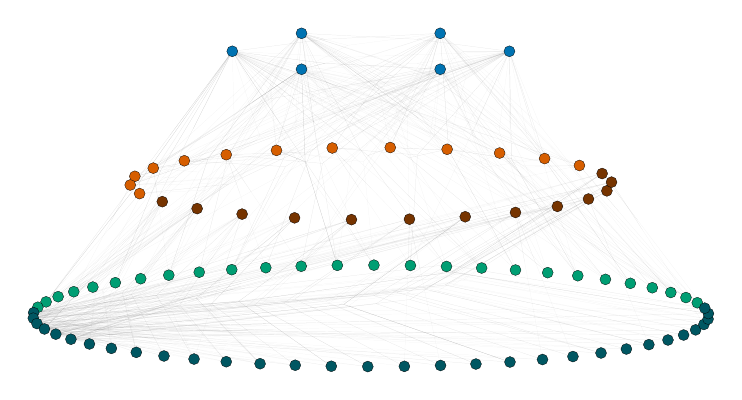
\begin{tikzpicture}[scale=1.4]
  \draw[gray, line width=0.08pt, opacity=0.10] (1.257,1.200) -- (0.419,1.309);
  \draw[gray, line width=0.08pt, opacity=0.10] (0.629,1.363) -- (0.419,1.309);
  \draw[gray, line width=0.08pt, opacity=0.10] (-0.629,1.363) -- (0.419,1.309);
  \draw[gray, line width=0.08pt, opacity=0.10] (1.257,1.200) -- (-0.210,1.146);
  \draw[gray, line width=0.08pt, opacity=0.10] (-1.257,1.200) -- (-0.210,1.146);
  \draw[gray, line width=0.08pt, opacity=0.10] (-0.629,1.037) -- (-0.210,1.146);
  \draw[gray, line width=0.08pt, opacity=0.10] (1.257,1.200) -- (0.838,1.200);
  \draw[gray, line width=0.08pt, opacity=0.10] (0.629,1.037) -- (0.838,1.200);
  \draw[gray, line width=0.08pt, opacity=0.10] (0.629,1.363) -- (0.838,1.200);
  \draw[gray, line width=0.08pt, opacity=0.10] (1.257,1.200) -- (0.859,0.958);
  \draw[gray, line width=0.08pt, opacity=0.10] (0.692,0.311) -- (0.859,0.958);
  \draw[gray, line width=0.08pt, opacity=0.10] (0.629,1.363) -- (0.859,0.958);
  \draw[gray, line width=0.08pt, opacity=0.10] (1.257,1.200) -- (1.275,0.225);
  \draw[gray, line width=0.08pt, opacity=0.10] (0.692,0.311) -- (1.275,0.225);
  \draw[gray, line width=0.08pt, opacity=0.10] (1.877,-0.836) -- (1.275,0.225);
  \draw[gray, line width=0.08pt, opacity=0.10] (1.257,1.200) -- (0.422,0.260);
  \draw[gray, line width=0.08pt, opacity=0.10] (-0.350,0.323) -- (0.422,0.260);
  \draw[gray, line width=0.08pt, opacity=0.10] (0.359,-0.743) -- (0.422,0.260);
  \draw[gray, line width=0.08pt, opacity=0.10] (1.257,1.200) -- (0.065,0.815);
  \draw[gray, line width=0.08pt, opacity=0.10] (-1.692,0.207) -- (0.065,0.815);
  \draw[gray, line width=0.08pt, opacity=0.10] (0.629,1.037) -- (0.065,0.815);
  \draw[gray, line width=0.08pt, opacity=0.10] (1.257,1.200) -- (-0.518,0.741);
  \draw[gray, line width=0.08pt, opacity=0.10] (-2.183,-0.013) -- (-0.518,0.741);
  \draw[gray, line width=0.08pt, opacity=0.10] (-0.629,1.037) -- (-0.518,0.741);
  \draw[gray, line width=0.08pt, opacity=0.10] (1.257,1.200) -- (-0.699,0.770);
  \draw[gray, line width=0.08pt, opacity=0.10] (-2.098,-0.091) -- (-0.699,0.770);
  \draw[gray, line width=0.08pt, opacity=0.10] (-1.257,1.200) -- (-0.699,0.770);
  \draw[gray, line width=0.08pt, opacity=0.10] (1.257,1.200) -- (1.464,0.521);
  \draw[gray, line width=0.08pt, opacity=0.10] (1.877,-0.836) -- (1.464,0.521);
  \draw[gray, line width=0.08pt, opacity=0.10] (1.257,1.200) -- (1.464,0.521);
  \draw[gray, line width=0.08pt, opacity=0.10] (1.257,1.200) -- (1.254,0.467);
  \draw[gray, line width=0.08pt, opacity=0.10] (1.877,-0.836) -- (1.254,0.467);
  \draw[gray, line width=0.08pt, opacity=0.10] (0.629,1.037) -- (1.254,0.467);
  \draw[gray, line width=0.08pt, opacity=0.10] (1.257,1.200) -- (0.329,0.607);
  \draw[gray, line width=0.08pt, opacity=0.10] (0.359,-0.743) -- (0.329,0.607);
  \draw[gray, line width=0.08pt, opacity=0.10] (-0.629,1.363) -- (0.329,0.607);
  \draw[gray, line width=0.08pt, opacity=0.10] (1.257,1.200) -- (-0.309,0.586);
  \draw[gray, line width=0.08pt, opacity=0.10] (-1.557,-0.804) -- (-0.309,0.586);
  \draw[gray, line width=0.08pt, opacity=0.10] (-0.629,1.363) -- (-0.309,0.586);
  \draw[gray, line width=0.08pt, opacity=0.10] (1.257,1.200) -- (-0.689,0.527);
  \draw[gray, line width=0.08pt, opacity=0.10] (-2.695,-0.981) -- (-0.689,0.527);
  \draw[gray, line width=0.08pt, opacity=0.10] (-0.629,1.363) -- (-0.689,0.527);
  \draw[gray, line width=0.08pt, opacity=0.10] (1.257,1.200) -- (-0.169,0.426);
  \draw[gray, line width=0.08pt, opacity=0.10] (-3.021,-1.122) -- (-0.169,0.426);
  \draw[gray, line width=0.08pt, opacity=0.10] (1.257,1.200) -- (-0.169,0.426);
  \draw[gray, line width=0.08pt, opacity=0.10] (1.257,1.200) -- (-1.287,-0.004);
  \draw[gray, line width=0.08pt, opacity=0.10] (-3.021,-1.122) -- (-1.287,-0.004);
  \draw[gray, line width=0.08pt, opacity=0.10] (-2.098,-0.091) -- (-1.287,-0.004);
  \draw[gray, line width=0.08pt, opacity=0.10] (0.629,1.363) -- (-0.419,1.309);
  \draw[gray, line width=0.08pt, opacity=0.10] (-0.629,1.363) -- (-0.419,1.309);
  \draw[gray, line width=0.08pt, opacity=0.10] (-1.257,1.200) -- (-0.419,1.309);
  \draw[gray, line width=0.08pt, opacity=0.10] (0.629,1.363) -- (1.154,0.930);
  \draw[gray, line width=0.08pt, opacity=0.10] (1.576,0.227) -- (1.154,0.930);
  \draw[gray, line width=0.08pt, opacity=0.10] (1.257,1.200) -- (1.154,0.930);
  \draw[gray, line width=0.08pt, opacity=0.10] (0.629,1.363) -- (1.642,0.201);
  \draw[gray, line width=0.08pt, opacity=0.10] (1.576,0.227) -- (1.642,0.201);
  \draw[gray, line width=0.08pt, opacity=0.10] (2.721,-0.988) -- (1.642,0.201);
  \draw[gray, line width=0.08pt, opacity=0.10] (0.629,1.363) -- (0.059,0.909);
  \draw[gray, line width=0.08pt, opacity=0.10] (0.176,0.327) -- (0.059,0.909);
  \draw[gray, line width=0.08pt, opacity=0.10] (-0.629,1.037) -- (0.059,0.909);
  \draw[gray, line width=0.08pt, opacity=0.10] (0.629,1.363) -- (-0.018,0.887);
  \draw[gray, line width=0.08pt, opacity=0.10] (-1.312,0.262) -- (-0.018,0.887);
  \draw[gray, line width=0.08pt, opacity=0.10] (0.629,1.037) -- (-0.018,0.887);
  \draw[gray, line width=0.08pt, opacity=0.10] (0.629,1.363) -- (-0.564,0.978);
  \draw[gray, line width=0.08pt, opacity=0.10] (-1.692,0.207) -- (-0.564,0.978);
  \draw[gray, line width=0.08pt, opacity=0.10] (-0.629,1.363) -- (-0.564,0.978);
  \draw[gray, line width=0.08pt, opacity=0.10] (0.629,1.363) -- (1.326,0.579);
  \draw[gray, line width=0.08pt, opacity=0.10] (2.721,-0.988) -- (1.326,0.579);
  \draw[gray, line width=0.08pt, opacity=0.10] (0.629,1.363) -- (1.326,0.579);
  \draw[gray, line width=0.08pt, opacity=0.10] (0.629,1.363) -- (0.857,0.647);
  \draw[gray, line width=0.08pt, opacity=0.10] (1.312,-0.784) -- (0.857,0.647);
  \draw[gray, line width=0.08pt, opacity=0.10] (0.629,1.363) -- (0.857,0.647);
  \draw[gray, line width=0.08pt, opacity=0.10] (0.629,1.363) -- (0.706,0.302);
  \draw[gray, line width=0.08pt, opacity=0.10] (1.312,-0.784) -- (0.706,0.302);
  \draw[gray, line width=0.08pt, opacity=0.10] (0.176,0.327) -- (0.706,0.302);
  \draw[gray, line width=0.08pt, opacity=0.10] (0.629,1.363) -- (-0.545,0.287);
  \draw[gray, line width=0.08pt, opacity=0.10] (-0.953,-0.763) -- (-0.545,0.287);
  \draw[gray, line width=0.08pt, opacity=0.10] (-1.312,0.262) -- (-0.545,0.287);
  \draw[gray, line width=0.08pt, opacity=0.10] (0.629,1.363) -- (-0.421,0.649);
  \draw[gray, line width=0.08pt, opacity=0.10] (-1.262,-0.781) -- (-0.421,0.649);
  \draw[gray, line width=0.08pt, opacity=0.10] (-0.629,1.363) -- (-0.421,0.649);
  \draw[gray, line width=0.08pt, opacity=0.10] (-0.629,1.363) -- (0.419,1.309);
  \draw[gray, line width=0.08pt, opacity=0.10] (0.629,1.363) -- (0.419,1.309);
  \draw[gray, line width=0.08pt, opacity=0.10] (1.257,1.200) -- (0.419,1.309);
  \draw[gray, line width=0.08pt, opacity=0.10] (-0.629,1.363) -- (-0.210,1.254);
  \draw[gray, line width=0.08pt, opacity=0.10] (-0.629,1.037) -- (-0.210,1.254);
  \draw[gray, line width=0.08pt, opacity=0.10] (0.629,1.363) -- (-0.210,1.254);
  \draw[gray, line width=0.08pt, opacity=0.10] (-0.629,1.363) -- (0.002,0.909);
  \draw[gray, line width=0.08pt, opacity=0.10] (1.892,0.164) -- (0.002,0.909);
  \draw[gray, line width=0.08pt, opacity=0.10] (-1.257,1.200) -- (0.002,0.909);
  \draw[gray, line width=0.08pt, opacity=0.10] (-0.629,1.363) -- (0.525,0.985);
  \draw[gray, line width=0.08pt, opacity=0.10] (1.576,0.227) -- (0.525,0.985);
  \draw[gray, line width=0.08pt, opacity=0.10] (0.629,1.363) -- (0.525,0.985);
  \draw[gray, line width=0.08pt, opacity=0.10] (-0.629,1.363) -- (0.093,0.962);
  \draw[gray, line width=0.08pt, opacity=0.10] (-0.350,0.323) -- (0.093,0.962);
  \draw[gray, line width=0.08pt, opacity=0.10] (1.257,1.200) -- (0.093,0.962);
  \draw[gray, line width=0.08pt, opacity=0.10] (-0.629,1.363) -- (-0.658,0.956);
  \draw[gray, line width=0.08pt, opacity=0.10] (-1.974,0.140) -- (-0.658,0.956);
  \draw[gray, line width=0.08pt, opacity=0.10] (0.629,1.363) -- (-0.658,0.956);
  \draw[gray, line width=0.08pt, opacity=0.10] (-0.629,1.363) -- (-1.478,0.224);
  \draw[gray, line width=0.08pt, opacity=0.10] (-1.974,0.140) -- (-1.478,0.224);
  \draw[gray, line width=0.08pt, opacity=0.10] (-1.833,-0.831) -- (-1.478,0.224);
  \draw[gray, line width=0.08pt, opacity=0.10] (-0.629,1.363) -- (0.534,0.455);
  \draw[gray, line width=0.08pt, opacity=0.10] (2.858,-1.034) -- (0.534,0.455);
  \draw[gray, line width=0.08pt, opacity=0.10] (-0.629,1.037) -- (0.534,0.455);
  \draw[gray, line width=0.08pt, opacity=0.10] (-0.629,1.363) -- (0.432,0.594);
  \draw[gray, line width=0.08pt, opacity=0.10] (2.553,-0.945) -- (0.432,0.594);
  \draw[gray, line width=0.08pt, opacity=0.10] (-0.629,1.363) -- (0.432,0.594);
  \draw[gray, line width=0.08pt, opacity=0.10] (-0.629,1.363) -- (0.229,0.658);
  \draw[gray, line width=0.08pt, opacity=0.10] (0.686,-0.752) -- (0.229,0.658);
  \draw[gray, line width=0.08pt, opacity=0.10] (0.629,1.363) -- (0.229,0.658);
  \draw[gray, line width=0.08pt, opacity=0.10] (-0.629,1.363) -- (-1.030,0.632);
  \draw[gray, line width=0.08pt, opacity=0.10] (-1.833,-0.831) -- (-1.030,0.632);
  \draw[gray, line width=0.08pt, opacity=0.10] (-0.629,1.363) -- (-1.030,0.632);
  \draw[gray, line width=0.08pt, opacity=0.10] (-1.257,1.200) -- (-0.419,1.309);
  \draw[gray, line width=0.08pt, opacity=0.10] (0.629,1.363) -- (-0.419,1.309);
  \draw[gray, line width=0.08pt, opacity=0.10] (-0.629,1.363) -- (-0.419,1.309);
  \draw[gray, line width=0.08pt, opacity=0.10] (-1.257,1.200) -- (-0.419,1.091);
  \draw[gray, line width=0.08pt, opacity=0.10] (-0.629,1.037) -- (-0.419,1.091);
  \draw[gray, line width=0.08pt, opacity=0.10] (0.629,1.037) -- (-0.419,1.091);
  \draw[gray, line width=0.08pt, opacity=0.10] (-1.257,1.200) -- (-0.208,0.855);
  \draw[gray, line width=0.08pt, opacity=0.10] (1.892,0.164) -- (-0.208,0.855);
  \draw[gray, line width=0.08pt, opacity=0.10] (-1.257,1.200) -- (-0.208,0.855);
  \draw[gray, line width=0.08pt, opacity=0.10] (-1.257,1.200) -- (-0.570,0.963);
  \draw[gray, line width=0.08pt, opacity=0.10] (0.176,0.327) -- (-0.570,0.963);
  \draw[gray, line width=0.08pt, opacity=0.10] (-0.629,1.363) -- (-0.570,0.963);
  \draw[gray, line width=0.08pt, opacity=0.10] (-1.257,1.200) -- (-0.914,0.955);
  \draw[gray, line width=0.08pt, opacity=0.10] (-0.856,0.301) -- (-0.914,0.955);
  \draw[gray, line width=0.08pt, opacity=0.10] (-0.629,1.363) -- (-0.914,0.955);
  \draw[gray, line width=0.08pt, opacity=0.10] (-1.257,1.200) -- (-0.695,0.254);
  \draw[gray, line width=0.08pt, opacity=0.10] (-0.856,0.301) -- (-0.695,0.254);
  \draw[gray, line width=0.08pt, opacity=0.10] (0.028,-0.740) -- (-0.695,0.254);
  \draw[gray, line width=0.08pt, opacity=0.10] (-1.257,1.200) -- (-1.905,0.122);
  \draw[gray, line width=0.08pt, opacity=0.10] (-2.141,0.066) -- (-1.905,0.122);
  \draw[gray, line width=0.08pt, opacity=0.10] (-2.318,-0.899) -- (-1.905,0.122);
  \draw[gray, line width=0.08pt, opacity=0.10] (-1.257,1.200) -- (-2.101,0.012);
  \draw[gray, line width=0.08pt, opacity=0.10] (-2.098,-0.091) -- (-2.101,0.012);
  \draw[gray, line width=0.08pt, opacity=0.10] (-2.946,-1.073) -- (-2.101,0.012);
  \draw[gray, line width=0.08pt, opacity=0.10] (-1.257,1.200) -- (0.358,0.385);
  \draw[gray, line width=0.08pt, opacity=0.10] (2.961,-1.081) -- (0.358,0.385);
  \draw[gray, line width=0.08pt, opacity=0.10] (-0.629,1.037) -- (0.358,0.385);
  \draw[gray, line width=0.08pt, opacity=0.10] (-1.257,1.200) -- (-0.503,0.545);
  \draw[gray, line width=0.08pt, opacity=0.10] (1.005,-0.766) -- (-0.503,0.545);
  \draw[gray, line width=0.08pt, opacity=0.10] (-1.257,1.200) -- (-0.503,0.545);
  \draw[gray, line width=0.08pt, opacity=0.10] (-1.257,1.200) -- (-0.829,0.553);
  \draw[gray, line width=0.08pt, opacity=0.10] (0.028,-0.740) -- (-0.829,0.553);
  \draw[gray, line width=0.08pt, opacity=0.10] (-1.257,1.200) -- (-0.829,0.553);
  \draw[gray, line width=0.08pt, opacity=0.10] (-1.257,1.200) -- (-1.611,0.500);
  \draw[gray, line width=0.08pt, opacity=0.10] (-2.318,-0.899) -- (-1.611,0.500);
  \draw[gray, line width=0.08pt, opacity=0.10] (-1.257,1.200) -- (-1.611,0.500);
  \draw[gray, line width=0.08pt, opacity=0.10] (-1.257,1.200) -- (-1.820,0.442);
  \draw[gray, line width=0.08pt, opacity=0.10] (-2.946,-1.073) -- (-1.820,0.442);
  \draw[gray, line width=0.08pt, opacity=0.10] (-1.257,1.200) -- (-1.820,0.442);
  \draw[gray, line width=0.08pt, opacity=0.10] (-1.257,1.200) -- (-2.101,0.012);
  \draw[gray, line width=0.08pt, opacity=0.10] (-2.946,-1.073) -- (-2.101,0.012);
  \draw[gray, line width=0.08pt, opacity=0.10] (-2.098,-0.091) -- (-2.101,0.012);
  \draw[gray, line width=0.08pt, opacity=0.10] (-0.629,1.037) -- (-0.419,1.091);
  \draw[gray, line width=0.08pt, opacity=0.10] (-1.257,1.200) -- (-0.419,1.091);
  \draw[gray, line width=0.08pt, opacity=0.10] (0.629,1.037) -- (-0.419,1.091);
  \draw[gray, line width=0.08pt, opacity=0.10] (-0.629,1.037) -- (-0.239,0.838);
  \draw[gray, line width=0.08pt, opacity=0.10] (1.168,0.277) -- (-0.239,0.838);
  \draw[gray, line width=0.08pt, opacity=0.10] (-1.257,1.200) -- (-0.239,0.838);
  \draw[gray, line width=0.08pt, opacity=0.10] (-0.629,1.037) -- (-0.705,0.900);
  \draw[gray, line width=0.08pt, opacity=0.10] (-0.856,0.301) -- (-0.705,0.900);
  \draw[gray, line width=0.08pt, opacity=0.10] (-0.629,1.363) -- (-0.705,0.900);
  \draw[gray, line width=0.08pt, opacity=0.10] (-0.629,1.037) -- (-0.596,0.199);
  \draw[gray, line width=0.08pt, opacity=0.10] (-0.856,0.301) -- (-0.596,0.199);
  \draw[gray, line width=0.08pt, opacity=0.10] (-0.304,-0.742) -- (-0.596,0.199);
  \draw[gray, line width=0.08pt, opacity=0.10] (-0.629,1.037) -- (-1.077,0.738);
  \draw[gray, line width=0.08pt, opacity=0.10] (-1.974,0.140) -- (-1.077,0.738);
  \draw[gray, line width=0.08pt, opacity=0.10] (-0.629,1.037) -- (-1.077,0.738);
  \draw[gray, line width=0.08pt, opacity=0.10] (-0.629,1.037) -- (-1.147,0.687);
  \draw[gray, line width=0.08pt, opacity=0.10] (-2.183,-0.013) -- (-1.147,0.687);
  \draw[gray, line width=0.08pt, opacity=0.10] (-0.629,1.037) -- (-1.147,0.687);
  \draw[gray, line width=0.08pt, opacity=0.10] (-0.629,1.037) -- (0.081,0.456);
  \draw[gray, line width=0.08pt, opacity=0.10] (2.128,-0.869) -- (0.081,0.456);
  \draw[gray, line width=0.08pt, opacity=0.10] (-1.257,1.200) -- (0.081,0.456);
  \draw[gray, line width=0.08pt, opacity=0.10] (-0.629,1.037) -- (-0.520,0.553);
  \draw[gray, line width=0.08pt, opacity=0.10] (-0.304,-0.742) -- (-0.520,0.553);
  \draw[gray, line width=0.08pt, opacity=0.10] (-0.629,1.363) -- (-0.520,0.553);
  \draw[gray, line width=0.08pt, opacity=0.10] (-0.629,1.037) -- (-0.596,0.199);
  \draw[gray, line width=0.08pt, opacity=0.10] (-0.304,-0.742) -- (-0.596,0.199);
  \draw[gray, line width=0.08pt, opacity=0.10] (-0.856,0.301) -- (-0.596,0.199);
  \draw[gray, line width=0.08pt, opacity=0.10] (-0.629,1.037) -- (-1.115,0.403);
  \draw[gray, line width=0.08pt, opacity=0.10] (-2.088,-0.863) -- (-1.115,0.403);
  \draw[gray, line width=0.08pt, opacity=0.10] (-0.629,1.037) -- (-1.115,0.403);
  \draw[gray, line width=0.08pt, opacity=0.10] (-0.629,1.037) -- (-1.365,0.349);
  \draw[gray, line width=0.08pt, opacity=0.10] (-2.837,-1.026) -- (-1.365,0.349);
  \draw[gray, line width=0.08pt, opacity=0.10] (-0.629,1.037) -- (-1.365,0.349);
  \draw[gray, line width=0.08pt, opacity=0.10] (0.629,1.037) -- (0.419,1.091);
  \draw[gray, line width=0.08pt, opacity=0.10] (1.257,1.200) -- (0.419,1.091);
  \draw[gray, line width=0.08pt, opacity=0.10] (-0.629,1.037) -- (0.419,1.091);
  \draw[gray, line width=0.08pt, opacity=0.10] (0.629,1.037) -- (-0.419,1.091);
  \draw[gray, line width=0.08pt, opacity=0.10] (-0.629,1.037) -- (-0.419,1.091);
  \draw[gray, line width=0.08pt, opacity=0.10] (-1.257,1.200) -- (-0.419,1.091);
  \draw[gray, line width=0.08pt, opacity=0.10] (0.629,1.037) -- (0.808,0.783);
  \draw[gray, line width=0.08pt, opacity=0.10] (1.168,0.277) -- (0.808,0.783);
  \draw[gray, line width=0.08pt, opacity=0.10] (0.629,1.037) -- (0.808,0.783);
  \draw[gray, line width=0.08pt, opacity=0.10] (0.629,1.037) -- (0.021,0.849);
  \draw[gray, line width=0.08pt, opacity=0.10] (0.692,0.311) -- (0.021,0.849);
  \draw[gray, line width=0.08pt, opacity=0.10] (-1.257,1.200) -- (0.021,0.849);
  \draw[gray, line width=0.08pt, opacity=0.10] (0.629,1.037) -- (0.191,0.833);
  \draw[gray, line width=0.08pt, opacity=0.10] (-1.312,0.262) -- (0.191,0.833);
  \draw[gray, line width=0.08pt, opacity=0.10] (1.257,1.200) -- (0.191,0.833);
  \draw[gray, line width=0.08pt, opacity=0.10] (0.629,1.037) -- (-0.923,0.767);
  \draw[gray, line width=0.08pt, opacity=0.10] (-2.141,0.066) -- (-0.923,0.767);
  \draw[gray, line width=0.08pt, opacity=0.10] (-1.257,1.200) -- (-0.923,0.767);
  \draw[gray, line width=0.08pt, opacity=0.10] (0.629,1.037) -- (1.413,0.444);
  \draw[gray, line width=0.08pt, opacity=0.10] (2.354,-0.905) -- (1.413,0.444);
  \draw[gray, line width=0.08pt, opacity=0.10] (1.257,1.200) -- (1.413,0.444);
  \draw[gray, line width=0.08pt, opacity=0.10] (0.629,1.037) -- (1.384,0.136);
  \draw[gray, line width=0.08pt, opacity=0.10] (2.354,-0.905) -- (1.384,0.136);
  \draw[gray, line width=0.08pt, opacity=0.10] (1.168,0.277) -- (1.384,0.136);
  \draw[gray, line width=0.08pt, opacity=0.10] (0.629,1.037) -- (0.535,0.422);
  \draw[gray, line width=0.08pt, opacity=0.10] (1.604,-0.808) -- (0.535,0.422);
  \draw[gray, line width=0.08pt, opacity=0.10] (-0.629,1.037) -- (0.535,0.422);
  \draw[gray, line width=0.08pt, opacity=0.10] (0.629,1.037) -- (0.208,0.550);
  \draw[gray, line width=0.08pt, opacity=0.10] (-0.632,-0.750) -- (0.208,0.550);
  \draw[gray, line width=0.08pt, opacity=0.10] (0.629,1.363) -- (0.208,0.550);
  \draw[gray, line width=0.08pt, opacity=0.10] (0.629,1.037) -- (-0.841,0.378);
  \draw[gray, line width=0.08pt, opacity=0.10] (-2.522,-0.939) -- (-0.841,0.378);
  \draw[gray, line width=0.08pt, opacity=0.10] (-0.629,1.037) -- (-0.841,0.378);
  \draw[gray, line width=0.08pt, opacity=0.10] (1.892,0.164) -- (0.212,0.964);
  \draw[gray, line width=0.08pt, opacity=0.10] (-0.629,1.363) -- (0.212,0.964);
  \draw[gray, line width=0.08pt, opacity=0.10] (-0.629,1.363) -- (0.212,0.964);
  \draw[gray, line width=0.08pt, opacity=0.10] (1.892,0.164) -- (1.374,0.165);
  \draw[gray, line width=0.08pt, opacity=0.10] (-0.629,1.363) -- (1.374,0.165);
  \draw[gray, line width=0.08pt, opacity=0.10] (2.858,-1.034) -- (1.374,0.165);
  \draw[gray, line width=0.08pt, opacity=0.10] (1.892,0.164) -- (-0.208,0.855);
  \draw[gray, line width=0.08pt, opacity=0.10] (-1.257,1.200) -- (-0.208,0.855);
  \draw[gray, line width=0.08pt, opacity=0.10] (-1.257,1.200) -- (-0.208,0.855);
  \draw[gray, line width=0.08pt, opacity=0.10] (1.892,0.164) -- (1.827,0.149);
  \draw[gray, line width=0.08pt, opacity=0.10] (2.961,-1.081) -- (1.827,0.149);
  \draw[gray, line width=0.08pt, opacity=0.10] (0.629,1.363) -- (1.827,0.149);
  \draw[gray, line width=0.08pt, opacity=0.10] (1.892,0.164) -- (2.248,-0.251);
  \draw[gray, line width=0.08pt, opacity=0.10] (2.961,-1.081) -- (2.248,-0.251);
  \draw[gray, line width=0.08pt, opacity=0.10] (1.892,0.164) -- (2.248,-0.251);
  \draw[gray, line width=0.08pt, opacity=0.10] (1.892,0.164) -- (1.374,0.056);
  \draw[gray, line width=0.08pt, opacity=0.10] (2.858,-1.034) -- (1.374,0.056);
  \draw[gray, line width=0.08pt, opacity=0.10] (-0.629,1.037) -- (1.374,0.056);
  \draw[gray, line width=0.08pt, opacity=0.10] (1.576,0.227) -- (0.525,0.985);
  \draw[gray, line width=0.08pt, opacity=0.10] (0.629,1.363) -- (0.525,0.985);
  \draw[gray, line width=0.08pt, opacity=0.10] (-0.629,1.363) -- (0.525,0.985);
  \draw[gray, line width=0.08pt, opacity=0.10] (1.576,0.227) -- (0.735,0.930);
  \draw[gray, line width=0.08pt, opacity=0.10] (-0.629,1.363) -- (0.735,0.930);
  \draw[gray, line width=0.08pt, opacity=0.10] (1.257,1.200) -- (0.735,0.930);
  \draw[gray, line width=0.08pt, opacity=0.10] (1.576,0.227) -- (0.841,0.606);
  \draw[gray, line width=0.08pt, opacity=0.10] (-0.629,1.363) -- (0.841,0.606);
  \draw[gray, line width=0.08pt, opacity=0.10] (1.576,0.227) -- (0.841,0.606);
  \draw[gray, line width=0.08pt, opacity=0.10] (1.576,0.227) -- (1.223,0.201);
  \draw[gray, line width=0.08pt, opacity=0.10] (2.721,-0.988) -- (1.223,0.201);
  \draw[gray, line width=0.08pt, opacity=0.10] (-0.629,1.363) -- (1.223,0.201);
  \draw[gray, line width=0.08pt, opacity=0.10] (1.576,0.227) -- (1.586,0.215);
  \draw[gray, line width=0.08pt, opacity=0.10] (2.553,-0.945) -- (1.586,0.215);
  \draw[gray, line width=0.08pt, opacity=0.10] (0.629,1.363) -- (1.586,0.215);
  \draw[gray, line width=0.08pt, opacity=0.10] (1.168,0.277) -- (0.599,0.838);
  \draw[gray, line width=0.08pt, opacity=0.10] (-0.629,1.037) -- (0.599,0.838);
  \draw[gray, line width=0.08pt, opacity=0.10] (1.257,1.200) -- (0.599,0.838);
  \draw[gray, line width=0.08pt, opacity=0.10] (1.168,0.277) -- (0.569,0.530);
  \draw[gray, line width=0.08pt, opacity=0.10] (-0.629,1.037) -- (0.569,0.530);
  \draw[gray, line width=0.08pt, opacity=0.10] (1.168,0.277) -- (0.569,0.530);
  \draw[gray, line width=0.08pt, opacity=0.10] (1.168,0.277) -- (0.389,0.783);
  \draw[gray, line width=0.08pt, opacity=0.10] (0.629,1.037) -- (0.389,0.783);
  \draw[gray, line width=0.08pt, opacity=0.10] (-0.629,1.037) -- (0.389,0.783);
  \draw[gray, line width=0.08pt, opacity=0.10] (1.168,0.277) -- (1.593,0.190);
  \draw[gray, line width=0.08pt, opacity=0.10] (2.354,-0.905) -- (1.593,0.190);
  \draw[gray, line width=0.08pt, opacity=0.10] (1.257,1.200) -- (1.593,0.190);
  \draw[gray, line width=0.08pt, opacity=0.10] (1.168,0.277) -- (1.563,-0.117);
  \draw[gray, line width=0.08pt, opacity=0.10] (2.354,-0.905) -- (1.563,-0.117);
  \draw[gray, line width=0.08pt, opacity=0.10] (1.168,0.277) -- (1.563,-0.117);
  \draw[gray, line width=0.08pt, opacity=0.10] (1.168,0.277) -- (1.308,0.148);
  \draw[gray, line width=0.08pt, opacity=0.10] (2.128,-0.869) -- (1.308,0.148);
  \draw[gray, line width=0.08pt, opacity=0.10] (0.629,1.037) -- (1.308,0.148);
  \draw[gray, line width=0.08pt, opacity=0.10] (0.692,0.311) -- (0.231,0.904);
  \draw[gray, line width=0.08pt, opacity=0.10] (1.257,1.200) -- (0.231,0.904);
  \draw[gray, line width=0.08pt, opacity=0.10] (-1.257,1.200) -- (0.231,0.904);
  \draw[gray, line width=0.08pt, opacity=0.10] (0.692,0.311) -- (1.275,0.225);
  \draw[gray, line width=0.08pt, opacity=0.10] (1.257,1.200) -- (1.275,0.225);
  \draw[gray, line width=0.08pt, opacity=0.10] (1.877,-0.836) -- (1.275,0.225);
  \draw[gray, line width=0.08pt, opacity=0.10] (0.692,0.311) -- (0.231,0.795);
  \draw[gray, line width=0.08pt, opacity=0.10] (0.629,1.037) -- (0.231,0.795);
  \draw[gray, line width=0.08pt, opacity=0.10] (-0.629,1.037) -- (0.231,0.795);
  \draw[gray, line width=0.08pt, opacity=0.10] (0.692,0.311) -- (1.275,0.225);
  \draw[gray, line width=0.08pt, opacity=0.10] (1.877,-0.836) -- (1.275,0.225);
  \draw[gray, line width=0.08pt, opacity=0.10] (1.257,1.200) -- (1.275,0.225);
  \draw[gray, line width=0.08pt, opacity=0.10] (0.692,0.311) -- (1.066,0.170);
  \draw[gray, line width=0.08pt, opacity=0.10] (1.877,-0.836) -- (1.066,0.170);
  \draw[gray, line width=0.08pt, opacity=0.10] (0.629,1.037) -- (1.066,0.170);
  \draw[gray, line width=0.08pt, opacity=0.10] (0.692,0.311) -- (0.346,0.234);
  \draw[gray, line width=0.08pt, opacity=0.10] (1.604,-0.808) -- (0.346,0.234);
  \draw[gray, line width=0.08pt, opacity=0.10] (-1.257,1.200) -- (0.346,0.234);
  \draw[gray, line width=0.08pt, opacity=0.10] (0.176,0.327) -- (0.478,1.018);
  \draw[gray, line width=0.08pt, opacity=0.10] (0.629,1.363) -- (0.478,1.018);
  \draw[gray, line width=0.08pt, opacity=0.10] (0.629,1.363) -- (0.478,1.018);
  \draw[gray, line width=0.08pt, opacity=0.10] (0.176,0.327) -- (0.327,0.672);
  \draw[gray, line width=0.08pt, opacity=0.10] (0.629,1.363) -- (0.327,0.672);
  \draw[gray, line width=0.08pt, opacity=0.10] (0.176,0.327) -- (0.327,0.672);
  \draw[gray, line width=0.08pt, opacity=0.10] (0.176,0.327) -- (-0.780,0.909);
  \draw[gray, line width=0.08pt, opacity=0.10] (-1.257,1.200) -- (-0.780,0.909);
  \draw[gray, line width=0.08pt, opacity=0.10] (-1.257,1.200) -- (-0.780,0.909);
  \draw[gray, line width=0.08pt, opacity=0.10] (0.176,0.327) -- (0.706,0.302);
  \draw[gray, line width=0.08pt, opacity=0.10] (1.312,-0.784) -- (0.706,0.302);
  \draw[gray, line width=0.08pt, opacity=0.10] (0.629,1.363) -- (0.706,0.302);
  \draw[gray, line width=0.08pt, opacity=0.10] (0.176,0.327) -- (0.286,0.193);
  \draw[gray, line width=0.08pt, opacity=0.10] (1.312,-0.784) -- (0.286,0.193);
  \draw[gray, line width=0.08pt, opacity=0.10] (-0.629,1.037) -- (0.286,0.193);
  \draw[gray, line width=0.08pt, opacity=0.10] (0.176,0.327) -- (-0.026,0.254);
  \draw[gray, line width=0.08pt, opacity=0.10] (1.005,-0.766) -- (-0.026,0.254);
  \draw[gray, line width=0.08pt, opacity=0.10] (-1.257,1.200) -- (-0.026,0.254);
  \draw[gray, line width=0.08pt, opacity=0.10] (-0.350,0.323) -- (0.512,0.962);
  \draw[gray, line width=0.08pt, opacity=0.10] (1.257,1.200) -- (0.512,0.962);
  \draw[gray, line width=0.08pt, opacity=0.10] (0.629,1.363) -- (0.512,0.962);
  \draw[gray, line width=0.08pt, opacity=0.10] (-0.350,0.323) -- (0.093,0.962);
  \draw[gray, line width=0.08pt, opacity=0.10] (-0.629,1.363) -- (0.093,0.962);
  \draw[gray, line width=0.08pt, opacity=0.10] (1.257,1.200) -- (0.093,0.962);
  \draw[gray, line width=0.08pt, opacity=0.10] (-0.350,0.323) -- (-0.098,0.312);
  \draw[gray, line width=0.08pt, opacity=0.10] (-0.629,1.363) -- (-0.098,0.312);
  \draw[gray, line width=0.08pt, opacity=0.10] (0.686,-0.752) -- (-0.098,0.312);
  \draw[gray, line width=0.08pt, opacity=0.10] (-0.350,0.323) -- (-0.005,-0.035);
  \draw[gray, line width=0.08pt, opacity=0.10] (0.686,-0.752) -- (-0.005,-0.035);
  \draw[gray, line width=0.08pt, opacity=0.10] (-0.350,0.323) -- (-0.005,-0.035);
  \draw[gray, line width=0.08pt, opacity=0.10] (-0.350,0.323) -- (-0.114,-0.032);
  \draw[gray, line width=0.08pt, opacity=0.10] (0.359,-0.743) -- (-0.114,-0.032);
  \draw[gray, line width=0.08pt, opacity=0.10] (-0.350,0.323) -- (-0.114,-0.032);
  \draw[gray, line width=0.08pt, opacity=0.10] (-0.856,0.301) -- (-0.495,0.846);
  \draw[gray, line width=0.08pt, opacity=0.10] (-1.257,1.200) -- (-0.495,0.846);
  \draw[gray, line width=0.08pt, opacity=0.10] (0.629,1.037) -- (-0.495,0.846);
  \draw[gray, line width=0.08pt, opacity=0.10] (-0.856,0.301) -- (-0.914,0.846);
  \draw[gray, line width=0.08pt, opacity=0.10] (-0.629,1.037) -- (-0.914,0.846);
  \draw[gray, line width=0.08pt, opacity=0.10] (-1.257,1.200) -- (-0.914,0.846);
  \draw[gray, line width=0.08pt, opacity=0.10] (-0.856,0.301) -- (-0.596,0.199);
  \draw[gray, line width=0.08pt, opacity=0.10] (-0.629,1.037) -- (-0.596,0.199);
  \draw[gray, line width=0.08pt, opacity=0.10] (-0.304,-0.742) -- (-0.596,0.199);
  \draw[gray, line width=0.08pt, opacity=0.10] (-0.856,0.301) -- (-0.067,0.199);
  \draw[gray, line width=0.08pt, opacity=0.10] (0.028,-0.740) -- (-0.067,0.199);
  \draw[gray, line width=0.08pt, opacity=0.10] (0.629,1.037) -- (-0.067,0.199);
  \draw[gray, line width=0.08pt, opacity=0.10] (-0.856,0.301) -- (-0.596,0.199);
  \draw[gray, line width=0.08pt, opacity=0.10] (-0.304,-0.742) -- (-0.596,0.199);
  \draw[gray, line width=0.08pt, opacity=0.10] (-0.629,1.037) -- (-0.596,0.199);
  \draw[gray, line width=0.08pt, opacity=0.10] (-1.312,0.262) -- (-0.018,0.996);
  \draw[gray, line width=0.08pt, opacity=0.10] (0.629,1.363) -- (-0.018,0.996);
  \draw[gray, line width=0.08pt, opacity=0.10] (0.629,1.363) -- (-0.018,0.996);
  \draw[gray, line width=0.08pt, opacity=0.10] (-1.312,0.262) -- (0.191,0.833);
  \draw[gray, line width=0.08pt, opacity=0.10] (0.629,1.037) -- (0.191,0.833);
  \draw[gray, line width=0.08pt, opacity=0.10] (1.257,1.200) -- (0.191,0.833);
  \draw[gray, line width=0.08pt, opacity=0.10] (-1.312,0.262) -- (-0.439,0.183);
  \draw[gray, line width=0.08pt, opacity=0.10] (0.629,1.037) -- (-0.439,0.183);
  \draw[gray, line width=0.08pt, opacity=0.10] (-0.632,-0.750) -- (-0.439,0.183);
  \draw[gray, line width=0.08pt, opacity=0.10] (-1.312,0.262) -- (-1.086,-0.075);
  \draw[gray, line width=0.08pt, opacity=0.10] (-0.632,-0.750) -- (-1.086,-0.075);
  \draw[gray, line width=0.08pt, opacity=0.10] (-1.312,0.262) -- (-1.086,-0.075);
  \draw[gray, line width=0.08pt, opacity=0.10] (-1.312,0.262) -- (-1.192,-0.080);
  \draw[gray, line width=0.08pt, opacity=0.10] (-0.953,-0.763) -- (-1.192,-0.080);
  \draw[gray, line width=0.08pt, opacity=0.10] (-1.312,0.262) -- (-1.192,-0.080);
  \draw[gray, line width=0.08pt, opacity=0.10] (-1.692,0.207) -- (0.065,0.815);
  \draw[gray, line width=0.08pt, opacity=0.10] (1.257,1.200) -- (0.065,0.815);
  \draw[gray, line width=0.08pt, opacity=0.10] (0.629,1.037) -- (0.065,0.815);
  \draw[gray, line width=0.08pt, opacity=0.10] (-1.692,0.207) -- (-0.145,0.978);
  \draw[gray, line width=0.08pt, opacity=0.10] (0.629,1.363) -- (-0.145,0.978);
  \draw[gray, line width=0.08pt, opacity=0.10] (0.629,1.363) -- (-0.145,0.978);
  \draw[gray, line width=0.08pt, opacity=0.10] (-1.692,0.207) -- (-0.775,0.263);
  \draw[gray, line width=0.08pt, opacity=0.10] (0.629,1.363) -- (-0.775,0.263);
  \draw[gray, line width=0.08pt, opacity=0.10] (-1.262,-0.781) -- (-0.775,0.263);
  \draw[gray, line width=0.08pt, opacity=0.10] (-1.692,0.207) -- (-0.775,0.154);
  \draw[gray, line width=0.08pt, opacity=0.10] (-1.262,-0.781) -- (-0.775,0.154);
  \draw[gray, line width=0.08pt, opacity=0.10] (0.629,1.037) -- (-0.775,0.154);
  \draw[gray, line width=0.08pt, opacity=0.10] (-1.692,0.207) -- (-1.293,0.256);
  \draw[gray, line width=0.08pt, opacity=0.10] (-1.557,-0.804) -- (-1.293,0.256);
  \draw[gray, line width=0.08pt, opacity=0.10] (-0.629,1.363) -- (-1.293,0.256);
  \draw[gray, line width=0.08pt, opacity=0.10] (-1.974,0.140) -- (-1.077,0.956);
  \draw[gray, line width=0.08pt, opacity=0.10] (-0.629,1.363) -- (-1.077,0.956);
  \draw[gray, line width=0.08pt, opacity=0.10] (-0.629,1.363) -- (-1.077,0.956);
  \draw[gray, line width=0.08pt, opacity=0.10] (-1.974,0.140) -- (-1.478,0.224);
  \draw[gray, line width=0.08pt, opacity=0.10] (-0.629,1.363) -- (-1.478,0.224);
  \draw[gray, line width=0.08pt, opacity=0.10] (-1.833,-0.831) -- (-1.478,0.224);
  \draw[gray, line width=0.08pt, opacity=0.10] (-1.974,0.140) -- (-1.077,0.738);
  \draw[gray, line width=0.08pt, opacity=0.10] (-0.629,1.037) -- (-1.077,0.738);
  \draw[gray, line width=0.08pt, opacity=0.10] (-0.629,1.037) -- (-1.077,0.738);
  \draw[gray, line width=0.08pt, opacity=0.10] (-1.974,0.140) -- (-1.059,0.224);
  \draw[gray, line width=0.08pt, opacity=0.10] (-1.833,-0.831) -- (-1.059,0.224);
  \draw[gray, line width=0.08pt, opacity=0.10] (0.629,1.363) -- (-1.059,0.224);
  \draw[gray, line width=0.08pt, opacity=0.10] (-1.974,0.140) -- (-1.927,-0.183);
  \draw[gray, line width=0.08pt, opacity=0.10] (-1.833,-0.831) -- (-1.927,-0.183);
  \draw[gray, line width=0.08pt, opacity=0.10] (-1.974,0.140) -- (-1.927,-0.183);
  \draw[gray, line width=0.08pt, opacity=0.10] (-1.974,0.140) -- (-1.563,0.105);
  \draw[gray, line width=0.08pt, opacity=0.10] (-2.088,-0.863) -- (-1.563,0.105);
  \draw[gray, line width=0.08pt, opacity=0.10] (-0.629,1.037) -- (-1.563,0.105);
  \draw[gray, line width=0.08pt, opacity=0.10] (-2.141,0.066) -- (-0.923,0.767);
  \draw[gray, line width=0.08pt, opacity=0.10] (-1.257,1.200) -- (-0.923,0.767);
  \draw[gray, line width=0.08pt, opacity=0.10] (0.629,1.037) -- (-0.923,0.767);
  \draw[gray, line width=0.08pt, opacity=0.10] (-2.141,0.066) -- (-0.714,0.713);
  \draw[gray, line width=0.08pt, opacity=0.10] (0.629,1.037) -- (-0.714,0.713);
  \draw[gray, line width=0.08pt, opacity=0.10] (-0.629,1.037) -- (-0.714,0.713);
  \draw[gray, line width=0.08pt, opacity=0.10] (-2.141,0.066) -- (-1.905,0.122);
  \draw[gray, line width=0.08pt, opacity=0.10] (-2.318,-0.899) -- (-1.905,0.122);
  \draw[gray, line width=0.08pt, opacity=0.10] (-1.257,1.200) -- (-1.905,0.122);
  \draw[gray, line width=0.08pt, opacity=0.10] (-2.141,0.066) -- (-1.973,0.109);
  \draw[gray, line width=0.08pt, opacity=0.10] (-2.522,-0.939) -- (-1.973,0.109);
  \draw[gray, line width=0.08pt, opacity=0.10] (-1.257,1.200) -- (-1.973,0.109);
  \draw[gray, line width=0.08pt, opacity=0.10] (-2.183,-0.013) -- (0.111,0.796);
  \draw[gray, line width=0.08pt, opacity=0.10] (1.257,1.200) -- (0.111,0.796);
  \draw[gray, line width=0.08pt, opacity=0.10] (1.257,1.200) -- (0.111,0.796);
  \draw[gray, line width=0.08pt, opacity=0.10] (-2.183,-0.013) -- (-1.036,0.391);
  \draw[gray, line width=0.08pt, opacity=0.10] (1.257,1.200) -- (-1.036,0.391);
  \draw[gray, line width=0.08pt, opacity=0.10] (-2.183,-0.013) -- (-1.036,0.391);
  \draw[gray, line width=0.08pt, opacity=0.10] (-2.183,-0.013) -- (-1.147,0.687);
  \draw[gray, line width=0.08pt, opacity=0.10] (-0.629,1.037) -- (-1.147,0.687);
  \draw[gray, line width=0.08pt, opacity=0.10] (-0.629,1.037) -- (-1.147,0.687);
  \draw[gray, line width=0.08pt, opacity=0.10] (-2.183,-0.013) -- (-1.207,0.069);
  \draw[gray, line width=0.08pt, opacity=0.10] (-2.695,-0.981) -- (-1.207,0.069);
  \draw[gray, line width=0.08pt, opacity=0.10] (1.257,1.200) -- (-1.207,0.069);
  \draw[gray, line width=0.08pt, opacity=0.10] (-2.183,-0.013) -- (-2.354,-0.336);
  \draw[gray, line width=0.08pt, opacity=0.10] (-2.695,-0.981) -- (-2.354,-0.336);
  \draw[gray, line width=0.08pt, opacity=0.10] (-2.183,-0.013) -- (-2.354,-0.336);
  \draw[gray, line width=0.08pt, opacity=0.10] (-2.183,-0.013) -- (-1.464,-0.001);
  \draw[gray, line width=0.08pt, opacity=0.10] (-2.837,-1.026) -- (-1.464,-0.001);
  \draw[gray, line width=0.08pt, opacity=0.10] (0.629,1.037) -- (-1.464,-0.001);
  \draw[gray, line width=0.08pt, opacity=0.10] (-2.098,-0.091) -- (-0.490,0.715);
  \draw[gray, line width=0.08pt, opacity=0.10] (1.257,1.200) -- (-0.490,0.715);
  \draw[gray, line width=0.08pt, opacity=0.10] (-0.629,1.037) -- (-0.490,0.715);
  \draw[gray, line width=0.08pt, opacity=0.10] (-2.098,-0.091) -- (-1.538,0.770);
  \draw[gray, line width=0.08pt, opacity=0.10] (-1.257,1.200) -- (-1.538,0.770);
  \draw[gray, line width=0.08pt, opacity=0.10] (-1.257,1.200) -- (-1.538,0.770);
  \draw[gray, line width=0.08pt, opacity=0.10] (-2.098,-0.091) -- (-2.101,0.012);
  \draw[gray, line width=0.08pt, opacity=0.10] (-1.257,1.200) -- (-2.101,0.012);
  \draw[gray, line width=0.08pt, opacity=0.10] (-2.946,-1.073) -- (-2.101,0.012);
  \draw[gray, line width=0.08pt, opacity=0.10] (-2.098,-0.091) -- (-2.381,-0.418);
  \draw[gray, line width=0.08pt, opacity=0.10] (-2.946,-1.073) -- (-2.381,-0.418);
  \draw[gray, line width=0.08pt, opacity=0.10] (-2.098,-0.091) -- (-2.381,-0.418);
  \draw[gray, line width=0.08pt, opacity=0.10] (-2.098,-0.091) -- (-1.497,-0.059);
  \draw[gray, line width=0.08pt, opacity=0.10] (-3.021,-1.122) -- (-1.497,-0.059);
  \draw[gray, line width=0.08pt, opacity=0.10] (0.629,1.037) -- (-1.497,-0.059);
  \draw[gray, line width=0.08pt, opacity=0.10] (2.961,-1.081) -- (0.149,0.440);
  \draw[gray, line width=0.08pt, opacity=0.10] (-1.257,1.200) -- (0.149,0.440);
  \draw[gray, line width=0.08pt, opacity=0.10] (-1.257,1.200) -- (0.149,0.440);
  \draw[gray, line width=0.08pt, opacity=0.10] (2.961,-1.081) -- (1.408,0.149);
  \draw[gray, line width=0.08pt, opacity=0.10] (1.892,0.164) -- (1.408,0.149);
  \draw[gray, line width=0.08pt, opacity=0.10] (-0.629,1.363) -- (1.408,0.149);
  \draw[gray, line width=0.08pt, opacity=0.10] (2.858,-1.034) -- (0.534,0.564);
  \draw[gray, line width=0.08pt, opacity=0.10] (-0.629,1.363) -- (0.534,0.564);
  \draw[gray, line width=0.08pt, opacity=0.10] (-0.629,1.363) -- (0.534,0.564);
  \draw[gray, line width=0.08pt, opacity=0.10] (2.858,-1.034) -- (1.793,0.165);
  \draw[gray, line width=0.08pt, opacity=0.10] (1.892,0.164) -- (1.793,0.165);
  \draw[gray, line width=0.08pt, opacity=0.10] (0.629,1.363) -- (1.793,0.165);
  \draw[gray, line width=0.08pt, opacity=0.10] (2.721,-0.988) -- (1.536,0.525);
  \draw[gray, line width=0.08pt, opacity=0.10] (0.629,1.363) -- (1.536,0.525);
  \draw[gray, line width=0.08pt, opacity=0.10] (1.257,1.200) -- (1.536,0.525);
  \draw[gray, line width=0.08pt, opacity=0.10] (2.721,-0.988) -- (1.642,0.201);
  \draw[gray, line width=0.08pt, opacity=0.10] (0.629,1.363) -- (1.642,0.201);
  \draw[gray, line width=0.08pt, opacity=0.10] (1.576,0.227) -- (1.642,0.201);
  \draw[gray, line width=0.08pt, opacity=0.10] (2.721,-0.988) -- (1.013,0.146);
  \draw[gray, line width=0.08pt, opacity=0.10] (1.576,0.227) -- (1.013,0.146);
  \draw[gray, line width=0.08pt, opacity=0.10] (-1.257,1.200) -- (1.013,0.146);
  \draw[gray, line width=0.08pt, opacity=0.10] (2.553,-0.945) -- (0.432,0.594);
  \draw[gray, line width=0.08pt, opacity=0.10] (-0.629,1.363) -- (0.432,0.594);
  \draw[gray, line width=0.08pt, opacity=0.10] (-0.629,1.363) -- (0.432,0.594);
  \draw[gray, line width=0.08pt, opacity=0.10] (2.553,-0.945) -- (1.586,0.215);
  \draw[gray, line width=0.08pt, opacity=0.10] (1.576,0.227) -- (1.586,0.215);
  \draw[gray, line width=0.08pt, opacity=0.10] (0.629,1.363) -- (1.586,0.215);
  \draw[gray, line width=0.08pt, opacity=0.10] (2.354,-0.905) -- (0.575,0.444);
  \draw[gray, line width=0.08pt, opacity=0.10] (0.629,1.037) -- (0.575,0.444);
  \draw[gray, line width=0.08pt, opacity=0.10] (-1.257,1.200) -- (0.575,0.444);
  \draw[gray, line width=0.08pt, opacity=0.10] (2.354,-0.905) -- (1.593,0.190);
  \draw[gray, line width=0.08pt, opacity=0.10] (1.168,0.277) -- (1.593,0.190);
  \draw[gray, line width=0.08pt, opacity=0.10] (1.257,1.200) -- (1.593,0.190);
  \draw[gray, line width=0.08pt, opacity=0.10] (2.128,-0.869) -- (0.919,0.456);
  \draw[gray, line width=0.08pt, opacity=0.10] (-0.629,1.037) -- (0.919,0.456);
  \draw[gray, line width=0.08pt, opacity=0.10] (1.257,1.200) -- (0.919,0.456);
  \draw[gray, line width=0.08pt, opacity=0.10] (2.128,-0.869) -- (0.889,0.148);
  \draw[gray, line width=0.08pt, opacity=0.10] (-0.629,1.037) -- (0.889,0.148);
  \draw[gray, line width=0.08pt, opacity=0.10] (1.168,0.277) -- (0.889,0.148);
  \draw[gray, line width=0.08pt, opacity=0.10] (2.128,-0.869) -- (1.308,0.148);
  \draw[gray, line width=0.08pt, opacity=0.10] (1.168,0.277) -- (1.308,0.148);
  \draw[gray, line width=0.08pt, opacity=0.10] (0.629,1.037) -- (1.308,0.148);
  \draw[gray, line width=0.08pt, opacity=0.10] (1.877,-0.836) -- (0.835,0.467);
  \draw[gray, line width=0.08pt, opacity=0.10] (1.257,1.200) -- (0.835,0.467);
  \draw[gray, line width=0.08pt, opacity=0.10] (-0.629,1.037) -- (0.835,0.467);
  \draw[gray, line width=0.08pt, opacity=0.10] (1.877,-0.836) -- (1.066,0.279);
  \draw[gray, line width=0.08pt, opacity=0.10] (0.692,0.311) -- (1.066,0.279);
  \draw[gray, line width=0.08pt, opacity=0.10] (0.629,1.363) -- (1.066,0.279);
  \draw[gray, line width=0.08pt, opacity=0.10] (1.604,-0.808) -- (1.163,0.476);
  \draw[gray, line width=0.08pt, opacity=0.10] (0.629,1.037) -- (1.163,0.476);
  \draw[gray, line width=0.08pt, opacity=0.10] (1.257,1.200) -- (1.163,0.476);
  \draw[gray, line width=0.08pt, opacity=0.10] (1.604,-0.808) -- (0.954,0.422);
  \draw[gray, line width=0.08pt, opacity=0.10] (0.629,1.037) -- (0.954,0.422);
  \draw[gray, line width=0.08pt, opacity=0.10] (0.629,1.037) -- (0.954,0.422);
  \draw[gray, line width=0.08pt, opacity=0.10] (1.604,-0.808) -- (0.346,0.234);
  \draw[gray, line width=0.08pt, opacity=0.10] (0.692,0.311) -- (0.346,0.234);
  \draw[gray, line width=0.08pt, opacity=0.10] (-1.257,1.200) -- (0.346,0.234);
  \draw[gray, line width=0.08pt, opacity=0.10] (1.312,-0.784) -- (0.437,0.647);
  \draw[gray, line width=0.08pt, opacity=0.10] (0.629,1.363) -- (0.437,0.647);
  \draw[gray, line width=0.08pt, opacity=0.10] (-0.629,1.363) -- (0.437,0.647);
  \draw[gray, line width=0.08pt, opacity=0.10] (1.312,-0.784) -- (0.706,0.302);
  \draw[gray, line width=0.08pt, opacity=0.10] (0.176,0.327) -- (0.706,0.302);
  \draw[gray, line width=0.08pt, opacity=0.10] (0.629,1.363) -- (0.706,0.302);
  \draw[gray, line width=0.08pt, opacity=0.10] (1.005,-0.766) -- (0.125,0.599);
  \draw[gray, line width=0.08pt, opacity=0.10] (-1.257,1.200) -- (0.125,0.599);
  \draw[gray, line width=0.08pt, opacity=0.10] (0.629,1.363) -- (0.125,0.599);
  \draw[gray, line width=0.08pt, opacity=0.10] (1.005,-0.766) -- (-0.026,0.254);
  \draw[gray, line width=0.08pt, opacity=0.10] (-1.257,1.200) -- (-0.026,0.254);
  \draw[gray, line width=0.08pt, opacity=0.10] (0.176,0.327) -- (-0.026,0.254);
  \draw[gray, line width=0.08pt, opacity=0.10] (1.005,-0.766) -- (0.184,0.199);
  \draw[gray, line width=0.08pt, opacity=0.10] (0.176,0.327) -- (0.184,0.199);
  \draw[gray, line width=0.08pt, opacity=0.10] (-0.629,1.037) -- (0.184,0.199);
  \draw[gray, line width=0.08pt, opacity=0.10] (0.686,-0.752) -- (-0.098,0.312);
  \draw[gray, line width=0.08pt, opacity=0.10] (-0.629,1.363) -- (-0.098,0.312);
  \draw[gray, line width=0.08pt, opacity=0.10] (-0.350,0.323) -- (-0.098,0.312);
  \draw[gray, line width=0.08pt, opacity=0.10] (0.359,-0.743) -- (0.958,0.552);
  \draw[gray, line width=0.08pt, opacity=0.10] (1.257,1.200) -- (0.958,0.552);
  \draw[gray, line width=0.08pt, opacity=0.10] (1.257,1.200) -- (0.958,0.552);
  \draw[gray, line width=0.08pt, opacity=0.10] (0.359,-0.743) -- (0.422,0.260);
  \draw[gray, line width=0.08pt, opacity=0.10] (-0.350,0.323) -- (0.422,0.260);
  \draw[gray, line width=0.08pt, opacity=0.10] (1.257,1.200) -- (0.422,0.260);
  \draw[gray, line width=0.08pt, opacity=0.10] (0.028,-0.740) -- (-0.829,0.553);
  \draw[gray, line width=0.08pt, opacity=0.10] (-1.257,1.200) -- (-0.829,0.553);
  \draw[gray, line width=0.08pt, opacity=0.10] (-1.257,1.200) -- (-0.829,0.553);
  \draw[gray, line width=0.08pt, opacity=0.10] (0.028,-0.740) -- (-0.486,0.308);
  \draw[gray, line width=0.08pt, opacity=0.10] (-0.856,0.301) -- (-0.486,0.308);
  \draw[gray, line width=0.08pt, opacity=0.10] (-0.629,1.363) -- (-0.486,0.308);
  \draw[gray, line width=0.08pt, opacity=0.10] (-0.304,-0.742) -- (-0.520,0.553);
  \draw[gray, line width=0.08pt, opacity=0.10] (-0.629,1.037) -- (-0.520,0.553);
  \draw[gray, line width=0.08pt, opacity=0.10] (-0.629,1.363) -- (-0.520,0.553);
  \draw[gray, line width=0.08pt, opacity=0.10] (-0.304,-0.742) -- (-0.596,0.199);
  \draw[gray, line width=0.08pt, opacity=0.10] (-0.629,1.037) -- (-0.596,0.199);
  \draw[gray, line width=0.08pt, opacity=0.10] (-0.856,0.301) -- (-0.596,0.199);
  \draw[gray, line width=0.08pt, opacity=0.10] (-0.304,-0.742) -- (-0.177,0.199);
  \draw[gray, line width=0.08pt, opacity=0.10] (-0.856,0.301) -- (-0.177,0.199);
  \draw[gray, line width=0.08pt, opacity=0.10] (0.629,1.037) -- (-0.177,0.199);
  \draw[gray, line width=0.08pt, opacity=0.10] (-0.632,-0.750) -- (0.208,0.441);
  \draw[gray, line width=0.08pt, opacity=0.10] (0.629,1.037) -- (0.208,0.441);
  \draw[gray, line width=0.08pt, opacity=0.10] (0.629,1.037) -- (0.208,0.441);
  \draw[gray, line width=0.08pt, opacity=0.10] (-0.632,-0.750) -- (-0.439,0.183);
  \draw[gray, line width=0.08pt, opacity=0.10] (-1.312,0.262) -- (-0.439,0.183);
  \draw[gray, line width=0.08pt, opacity=0.10] (0.629,1.037) -- (-0.439,0.183);
  \draw[gray, line width=0.08pt, opacity=0.10] (-0.953,-0.763) -- (-0.545,0.287);
  \draw[gray, line width=0.08pt, opacity=0.10] (0.629,1.363) -- (-0.545,0.287);
  \draw[gray, line width=0.08pt, opacity=0.10] (-1.312,0.262) -- (-0.545,0.287);
  \draw[gray, line width=0.08pt, opacity=0.10] (-1.262,-0.781) -- (0.208,0.594);
  \draw[gray, line width=0.08pt, opacity=0.10] (0.629,1.363) -- (0.208,0.594);
  \draw[gray, line width=0.08pt, opacity=0.10] (1.257,1.200) -- (0.208,0.594);
  \draw[gray, line width=0.08pt, opacity=0.10] (-1.262,-0.781) -- (-0.775,0.263);
  \draw[gray, line width=0.08pt, opacity=0.10] (0.629,1.363) -- (-0.775,0.263);
  \draw[gray, line width=0.08pt, opacity=0.10] (-1.692,0.207) -- (-0.775,0.263);
  \draw[gray, line width=0.08pt, opacity=0.10] (-1.262,-0.781) -- (-0.775,0.154);
  \draw[gray, line width=0.08pt, opacity=0.10] (-1.692,0.207) -- (-0.775,0.154);
  \draw[gray, line width=0.08pt, opacity=0.10] (0.629,1.037) -- (-0.775,0.154);
  \draw[gray, line width=0.08pt, opacity=0.10] (-1.557,-0.804) -- (0.110,0.478);
  \draw[gray, line width=0.08pt, opacity=0.10] (1.257,1.200) -- (0.110,0.478);
  \draw[gray, line width=0.08pt, opacity=0.10] (0.629,1.037) -- (0.110,0.478);
  \draw[gray, line width=0.08pt, opacity=0.10] (-1.557,-0.804) -- (-1.293,0.256);
  \draw[gray, line width=0.08pt, opacity=0.10] (-1.692,0.207) -- (-1.293,0.256);
  \draw[gray, line width=0.08pt, opacity=0.10] (-0.629,1.363) -- (-1.293,0.256);
  \draw[gray, line width=0.08pt, opacity=0.10] (-1.833,-0.831) -- (-1.240,0.577);
  \draw[gray, line width=0.08pt, opacity=0.10] (-0.629,1.363) -- (-1.240,0.577);
  \draw[gray, line width=0.08pt, opacity=0.10] (-1.257,1.200) -- (-1.240,0.577);
  \draw[gray, line width=0.08pt, opacity=0.10] (-1.833,-0.831) -- (-1.478,0.224);
  \draw[gray, line width=0.08pt, opacity=0.10] (-1.974,0.140) -- (-1.478,0.224);
  \draw[gray, line width=0.08pt, opacity=0.10] (-0.629,1.363) -- (-1.478,0.224);
  \draw[gray, line width=0.08pt, opacity=0.10] (-2.088,-0.863) -- (-1.115,0.512);
  \draw[gray, line width=0.08pt, opacity=0.10] (-0.629,1.037) -- (-1.115,0.512);
  \draw[gray, line width=0.08pt, opacity=0.10] (-0.629,1.363) -- (-1.115,0.512);
  \draw[gray, line width=0.08pt, opacity=0.10] (-2.088,-0.863) -- (-1.144,0.213);
  \draw[gray, line width=0.08pt, opacity=0.10] (-1.974,0.140) -- (-1.144,0.213);
  \draw[gray, line width=0.08pt, opacity=0.10] (0.629,1.363) -- (-1.144,0.213);
  \draw[gray, line width=0.08pt, opacity=0.10] (-2.318,-0.899) -- (-1.611,0.500);
  \draw[gray, line width=0.08pt, opacity=0.10] (-1.257,1.200) -- (-1.611,0.500);
  \draw[gray, line width=0.08pt, opacity=0.10] (-1.257,1.200) -- (-1.611,0.500);
  \draw[gray, line width=0.08pt, opacity=0.10] (-2.318,-0.899) -- (-1.905,0.122);
  \draw[gray, line width=0.08pt, opacity=0.10] (-2.141,0.066) -- (-1.905,0.122);
  \draw[gray, line width=0.08pt, opacity=0.10] (-1.257,1.200) -- (-1.905,0.122);
  \draw[gray, line width=0.08pt, opacity=0.10] (-2.522,-0.939) -- (-0.841,0.378);
  \draw[gray, line width=0.08pt, opacity=0.10] (0.629,1.037) -- (-0.841,0.378);
  \draw[gray, line width=0.08pt, opacity=0.10] (-0.629,1.037) -- (-0.841,0.378);
  \draw[gray, line width=0.08pt, opacity=0.10] (-2.522,-0.939) -- (-1.764,0.055);
  \draw[gray, line width=0.08pt, opacity=0.10] (-2.141,0.066) -- (-1.764,0.055);
  \draw[gray, line width=0.08pt, opacity=0.10] (-0.629,1.037) -- (-1.764,0.055);
  \draw[gray, line width=0.08pt, opacity=0.10] (-2.695,-0.981) -- (-0.689,0.419);
  \draw[gray, line width=0.08pt, opacity=0.10] (1.257,1.200) -- (-0.689,0.419);
  \draw[gray, line width=0.08pt, opacity=0.10] (-0.629,1.037) -- (-0.689,0.419);
  \draw[gray, line width=0.08pt, opacity=0.10] (-2.695,-0.981) -- (-1.836,0.123);
  \draw[gray, line width=0.08pt, opacity=0.10] (-2.183,-0.013) -- (-1.836,0.123);
  \draw[gray, line width=0.08pt, opacity=0.10] (-0.629,1.363) -- (-1.836,0.123);
  \draw[gray, line width=0.08pt, opacity=0.10] (-2.837,-1.026) -- (-1.365,0.458);
  \draw[gray, line width=0.08pt, opacity=0.10] (-0.629,1.037) -- (-1.365,0.458);
  \draw[gray, line width=0.08pt, opacity=0.10] (-0.629,1.363) -- (-1.365,0.458);
  \draw[gray, line width=0.08pt, opacity=0.10] (-2.837,-1.026) -- (-1.254,0.054);
  \draw[gray, line width=0.08pt, opacity=0.10] (-2.183,-0.013) -- (-1.254,0.054);
  \draw[gray, line width=0.08pt, opacity=0.10] (1.257,1.200) -- (-1.254,0.054);
  \draw[gray, line width=0.08pt, opacity=0.10] (-2.946,-1.073) -- (-1.820,0.442);
  \draw[gray, line width=0.08pt, opacity=0.10] (-1.257,1.200) -- (-1.820,0.442);
  \draw[gray, line width=0.08pt, opacity=0.10] (-1.257,1.200) -- (-1.820,0.442);
  \draw[gray, line width=0.08pt, opacity=0.10] (-2.946,-1.073) -- (-2.101,0.012);
  \draw[gray, line width=0.08pt, opacity=0.10] (-2.098,-0.091) -- (-2.101,0.012);
  \draw[gray, line width=0.08pt, opacity=0.10] (-1.257,1.200) -- (-2.101,0.012);
  \draw[gray, line width=0.08pt, opacity=0.10] (-3.021,-1.122) -- (-1.007,0.426);
  \draw[gray, line width=0.08pt, opacity=0.10] (1.257,1.200) -- (-1.007,0.426);
  \draw[gray, line width=0.08pt, opacity=0.10] (-1.257,1.200) -- (-1.007,0.426);
  \draw[gray, line width=0.08pt, opacity=0.10] (-3.021,-1.122) -- (-1.287,-0.004);
  \draw[gray, line width=0.08pt, opacity=0.10] (-2.098,-0.091) -- (-1.287,-0.004);
  \draw[gray, line width=0.08pt, opacity=0.10] (1.257,1.200) -- (-1.287,-0.004);
  \draw[gray, line width=0.08pt, opacity=0.10] (-3.059,-1.171) -- (-3.050,-1.221);
  \draw[gray, line width=0.08pt, opacity=0.10] (-3.062,-1.221) -- (-3.050,-1.221);
  \draw[gray, line width=0.08pt, opacity=0.10] (-3.029,-1.270) -- (-3.050,-1.221);
  \draw[gray, line width=0.08pt, opacity=0.10] (-3.059,-1.171) -- (-2.959,-1.285);
  \draw[gray, line width=0.08pt, opacity=0.10] (-2.961,-1.319) -- (-2.959,-1.285);
  \draw[gray, line width=0.08pt, opacity=0.10] (-2.858,-1.366) -- (-2.959,-1.285);
  \draw[gray, line width=0.08pt, opacity=0.10] (-3.059,-1.171) -- (-2.948,-1.268);
  \draw[gray, line width=0.08pt, opacity=0.10] (-2.721,-1.412) -- (-2.948,-1.268);
  \draw[gray, line width=0.08pt, opacity=0.10] (-3.062,-1.221) -- (-2.948,-1.268);
  \draw[gray, line width=0.08pt, opacity=0.10] (-3.059,-1.171) -- (-2.271,-0.901);
  \draw[gray, line width=0.08pt, opacity=0.10] (-0.692,-0.311) -- (-2.271,-0.901);
  \draw[gray, line width=0.08pt, opacity=0.10] (-3.062,-1.221) -- (-2.271,-0.901);
  \draw[gray, line width=0.08pt, opacity=0.10] (-3.059,-1.171) -- (-1.585,-1.039);
  \draw[gray, line width=0.08pt, opacity=0.10] (-0.692,-0.311) -- (-1.585,-1.039);
  \draw[gray, line width=0.08pt, opacity=0.10] (-1.005,-1.634) -- (-1.585,-1.039);
  \draw[gray, line width=0.08pt, opacity=0.10] (-3.059,-1.171) -- (-0.692,-1.048);
  \draw[gray, line width=0.08pt, opacity=0.10] (0.350,-0.323) -- (-0.692,-1.048);
  \draw[gray, line width=0.08pt, opacity=0.10] (0.632,-1.650) -- (-0.692,-1.048);
  \draw[gray, line width=0.08pt, opacity=0.10] (-3.059,-1.171) -- (-1.363,-0.930);
  \draw[gray, line width=0.08pt, opacity=0.10] (1.692,-0.207) -- (-1.363,-0.930);
  \draw[gray, line width=0.08pt, opacity=0.10] (-2.721,-1.412) -- (-1.363,-0.930);
  \draw[gray, line width=0.08pt, opacity=0.10] (-3.059,-1.171) -- (-1.245,-0.841);
  \draw[gray, line width=0.08pt, opacity=0.10] (2.183,0.013) -- (-1.245,-0.841);
  \draw[gray, line width=0.08pt, opacity=0.10] (-2.858,-1.366) -- (-1.245,-0.841);
  \draw[gray, line width=0.08pt, opacity=0.10] (-3.059,-1.171) -- (-1.307,-0.800);
  \draw[gray, line width=0.08pt, opacity=0.10] (2.098,0.091) -- (-1.307,-0.800);
  \draw[gray, line width=0.08pt, opacity=0.10] (-2.961,-1.319) -- (-1.307,-0.800);
  \draw[gray, line width=0.08pt, opacity=0.10] (-3.059,-1.171) -- (-2.375,-1.325);
  \draw[gray, line width=0.08pt, opacity=0.10] (-1.005,-1.634) -- (-2.375,-1.325);
  \draw[gray, line width=0.08pt, opacity=0.10] (-3.059,-1.171) -- (-2.375,-1.325);
  \draw[gray, line width=0.08pt, opacity=0.10] (-3.059,-1.171) -- (-2.262,-1.406);
  \draw[gray, line width=0.08pt, opacity=0.10] (-1.005,-1.634) -- (-2.262,-1.406);
  \draw[gray, line width=0.08pt, opacity=0.10] (-2.721,-1.412) -- (-2.262,-1.406);
  \draw[gray, line width=0.08pt, opacity=0.10] (-3.059,-1.171) -- (-1.819,-1.364);
  \draw[gray, line width=0.08pt, opacity=0.10] (0.632,-1.650) -- (-1.819,-1.364);
  \draw[gray, line width=0.08pt, opacity=0.10] (-3.029,-1.270) -- (-1.819,-1.364);
  \draw[gray, line width=0.08pt, opacity=0.10] (-3.059,-1.171) -- (-1.257,-1.314);
  \draw[gray, line width=0.08pt, opacity=0.10] (2.318,-1.501) -- (-1.257,-1.314);
  \draw[gray, line width=0.08pt, opacity=0.10] (-3.029,-1.270) -- (-1.257,-1.314);
  \draw[gray, line width=0.08pt, opacity=0.10] (-3.059,-1.171) -- (-1.023,-1.240);
  \draw[gray, line width=0.08pt, opacity=0.10] (3.021,-1.278) -- (-1.023,-1.240);
  \draw[gray, line width=0.08pt, opacity=0.10] (-3.029,-1.270) -- (-1.023,-1.240);
  \draw[gray, line width=0.08pt, opacity=0.10] (-3.059,-1.171) -- (-1.030,-1.157);
  \draw[gray, line width=0.08pt, opacity=0.10] (3.029,-1.130) -- (-1.030,-1.157);
  \draw[gray, line width=0.08pt, opacity=0.10] (-3.059,-1.171) -- (-1.030,-1.157);
  \draw[gray, line width=0.08pt, opacity=0.10] (-3.059,-1.171) -- (0.689,-0.736);
  \draw[gray, line width=0.08pt, opacity=0.10] (3.029,-1.130) -- (0.689,-0.736);
  \draw[gray, line width=0.08pt, opacity=0.10] (2.098,0.091) -- (0.689,-0.736);
  \draw[gray, line width=0.08pt, opacity=0.10] (-3.062,-1.221) -- (-3.018,-1.270);
  \draw[gray, line width=0.08pt, opacity=0.10] (-3.029,-1.270) -- (-3.018,-1.270);
  \draw[gray, line width=0.08pt, opacity=0.10] (-2.961,-1.319) -- (-3.018,-1.270);
  \draw[gray, line width=0.08pt, opacity=0.10] (-3.062,-1.221) -- (-2.566,-0.873);
  \draw[gray, line width=0.08pt, opacity=0.10] (-1.576,-0.227) -- (-2.566,-0.873);
  \draw[gray, line width=0.08pt, opacity=0.10] (-3.059,-1.171) -- (-2.566,-0.873);
  \draw[gray, line width=0.08pt, opacity=0.10] (-3.062,-1.221) -- (-2.255,-0.993);
  \draw[gray, line width=0.08pt, opacity=0.10] (-1.576,-0.227) -- (-2.255,-0.993);
  \draw[gray, line width=0.08pt, opacity=0.10] (-2.128,-1.531) -- (-2.255,-0.993);
  \draw[gray, line width=0.08pt, opacity=0.10] (-3.062,-1.221) -- (-2.032,-0.971);
  \draw[gray, line width=0.08pt, opacity=0.10] (-0.176,-0.327) -- (-2.032,-0.971);
  \draw[gray, line width=0.08pt, opacity=0.10] (-2.858,-1.366) -- (-2.032,-0.971);
  \draw[gray, line width=0.08pt, opacity=0.10] (-3.062,-1.221) -- (-1.490,-0.965);
  \draw[gray, line width=0.08pt, opacity=0.10] (1.312,-0.262) -- (-1.490,-0.965);
  \draw[gray, line width=0.08pt, opacity=0.10] (-2.721,-1.412) -- (-1.490,-0.965);
  \draw[gray, line width=0.08pt, opacity=0.10] (-3.062,-1.221) -- (-1.467,-0.899);
  \draw[gray, line width=0.08pt, opacity=0.10] (1.692,-0.207) -- (-1.467,-0.899);
  \draw[gray, line width=0.08pt, opacity=0.10] (-3.029,-1.270) -- (-1.467,-0.899);
  \draw[gray, line width=0.08pt, opacity=0.10] (-3.062,-1.221) -- (-2.751,-1.324);
  \draw[gray, line width=0.08pt, opacity=0.10] (-2.128,-1.531) -- (-2.751,-1.324);
  \draw[gray, line width=0.08pt, opacity=0.10] (-3.062,-1.221) -- (-2.751,-1.324);
  \draw[gray, line width=0.08pt, opacity=0.10] (-3.062,-1.221) -- (-2.161,-1.366);
  \draw[gray, line width=0.08pt, opacity=0.10] (-0.359,-1.657) -- (-2.161,-1.366);
  \draw[gray, line width=0.08pt, opacity=0.10] (-3.062,-1.221) -- (-2.161,-1.366);
  \draw[gray, line width=0.08pt, opacity=0.10] (-3.062,-1.221) -- (-1.199,-1.068);
  \draw[gray, line width=0.08pt, opacity=0.10] (-0.359,-1.657) -- (-1.199,-1.068);
  \draw[gray, line width=0.08pt, opacity=0.10] (-0.176,-0.327) -- (-1.199,-1.068);
  \draw[gray, line width=0.08pt, opacity=0.10] (-3.062,-1.221) -- (0.028,-1.017);
  \draw[gray, line width=0.08pt, opacity=0.10] (1.833,-1.569) -- (0.028,-1.017);
  \draw[gray, line width=0.08pt, opacity=0.10] (1.312,-0.262) -- (0.028,-1.017);
  \draw[gray, line width=0.08pt, opacity=0.10] (-3.062,-1.221) -- (-1.335,-1.343);
  \draw[gray, line width=0.08pt, opacity=0.10] (2.088,-1.537) -- (-1.335,-1.343);
  \draw[gray, line width=0.08pt, opacity=0.10] (-3.029,-1.270) -- (-1.335,-1.343);
  \draw[gray, line width=0.08pt, opacity=0.10] (-3.029,-1.270) -- (-3.050,-1.221);
  \draw[gray, line width=0.08pt, opacity=0.10] (-3.062,-1.221) -- (-3.050,-1.221);
  \draw[gray, line width=0.08pt, opacity=0.10] (-3.059,-1.171) -- (-3.050,-1.221);
  \draw[gray, line width=0.08pt, opacity=0.10] (-3.029,-1.270) -- (-2.983,-1.286);
  \draw[gray, line width=0.08pt, opacity=0.10] (-2.858,-1.366) -- (-2.983,-1.286);
  \draw[gray, line width=0.08pt, opacity=0.10] (-3.062,-1.221) -- (-2.983,-1.286);
  \draw[gray, line width=0.08pt, opacity=0.10] (-3.029,-1.270) -- (-2.628,-0.918);
  \draw[gray, line width=0.08pt, opacity=0.10] (-1.892,-0.164) -- (-2.628,-0.918);
  \draw[gray, line width=0.08pt, opacity=0.10] (-2.961,-1.319) -- (-2.628,-0.918);
  \draw[gray, line width=0.08pt, opacity=0.10] (-3.029,-1.270) -- (-2.556,-0.906);
  \draw[gray, line width=0.08pt, opacity=0.10] (-1.576,-0.227) -- (-2.556,-0.906);
  \draw[gray, line width=0.08pt, opacity=0.10] (-3.062,-1.221) -- (-2.556,-0.906);
  \draw[gray, line width=0.08pt, opacity=0.10] (-3.029,-1.270) -- (-1.913,-0.922);
  \draw[gray, line width=0.08pt, opacity=0.10] (0.350,-0.323) -- (-1.913,-0.922);
  \draw[gray, line width=0.08pt, opacity=0.10] (-3.059,-1.171) -- (-1.913,-0.922);
  \draw[gray, line width=0.08pt, opacity=0.10] (-3.029,-1.270) -- (-1.373,-0.877);
  \draw[gray, line width=0.08pt, opacity=0.10] (1.974,-0.140) -- (-1.373,-0.877);
  \draw[gray, line width=0.08pt, opacity=0.10] (-3.062,-1.221) -- (-1.373,-0.877);
  \draw[gray, line width=0.08pt, opacity=0.10] (-3.029,-1.270) -- (0.489,-0.957);
  \draw[gray, line width=0.08pt, opacity=0.10] (1.974,-0.140) -- (0.489,-0.957);
  \draw[gray, line width=0.08pt, opacity=0.10] (2.522,-1.461) -- (0.489,-0.957);
  \draw[gray, line width=0.08pt, opacity=0.10] (-3.029,-1.270) -- (-2.747,-1.377);
  \draw[gray, line width=0.08pt, opacity=0.10] (-2.354,-1.495) -- (-2.747,-1.377);
  \draw[gray, line width=0.08pt, opacity=0.10] (-2.858,-1.366) -- (-2.747,-1.377);
  \draw[gray, line width=0.08pt, opacity=0.10] (-3.029,-1.270) -- (-2.645,-1.368);
  \draw[gray, line width=0.08pt, opacity=0.10] (-1.877,-1.564) -- (-2.645,-1.368);
  \draw[gray, line width=0.08pt, opacity=0.10] (-3.029,-1.270) -- (-2.645,-1.368);
  \draw[gray, line width=0.08pt, opacity=0.10] (-3.029,-1.270) -- (-1.929,-1.383);
  \draw[gray, line width=0.08pt, opacity=0.10] (0.304,-1.658) -- (-1.929,-1.383);
  \draw[gray, line width=0.08pt, opacity=0.10] (-3.062,-1.221) -- (-1.929,-1.383);
  \draw[gray, line width=0.08pt, opacity=0.10] (-3.029,-1.270) -- (-1.179,-1.334);
  \draw[gray, line width=0.08pt, opacity=0.10] (2.522,-1.461) -- (-1.179,-1.334);
  \draw[gray, line width=0.08pt, opacity=0.10] (-3.029,-1.270) -- (-1.179,-1.334);
  \draw[gray, line width=0.08pt, opacity=0.10] (-2.961,-1.319) -- (-3.018,-1.270);
  \draw[gray, line width=0.08pt, opacity=0.10] (-3.062,-1.221) -- (-3.018,-1.270);
  \draw[gray, line width=0.08pt, opacity=0.10] (-3.029,-1.270) -- (-3.018,-1.270);
  \draw[gray, line width=0.08pt, opacity=0.10] (-2.961,-1.319) -- (-2.847,-1.366);
  \draw[gray, line width=0.08pt, opacity=0.10] (-2.858,-1.366) -- (-2.847,-1.366);
  \draw[gray, line width=0.08pt, opacity=0.10] (-2.721,-1.412) -- (-2.847,-1.366);
  \draw[gray, line width=0.08pt, opacity=0.10] (-2.961,-1.319) -- (-2.605,-0.934);
  \draw[gray, line width=0.08pt, opacity=0.10] (-1.892,-0.164) -- (-2.605,-0.934);
  \draw[gray, line width=0.08pt, opacity=0.10] (-2.961,-1.319) -- (-2.605,-0.934);
  \draw[gray, line width=0.08pt, opacity=0.10] (-2.961,-1.319) -- (-2.055,-0.972);
  \draw[gray, line width=0.08pt, opacity=0.10] (-0.176,-0.327) -- (-2.055,-0.972);
  \draw[gray, line width=0.08pt, opacity=0.10] (-3.029,-1.270) -- (-2.055,-0.972);
  \draw[gray, line width=0.08pt, opacity=0.10] (-2.961,-1.319) -- (-1.711,-0.964);
  \draw[gray, line width=0.08pt, opacity=0.10] (0.856,-0.301) -- (-1.711,-0.964);
  \draw[gray, line width=0.08pt, opacity=0.10] (-3.029,-1.270) -- (-1.711,-0.964);
  \draw[gray, line width=0.08pt, opacity=0.10] (-2.961,-1.319) -- (-0.384,-1.086);
  \draw[gray, line width=0.08pt, opacity=0.10] (0.856,-0.301) -- (-0.384,-1.086);
  \draw[gray, line width=0.08pt, opacity=0.10] (0.953,-1.637) -- (-0.384,-1.086);
  \draw[gray, line width=0.08pt, opacity=0.10] (-2.961,-1.319) -- (0.672,-0.920);
  \draw[gray, line width=0.08pt, opacity=0.10] (2.141,-0.066) -- (0.672,-0.920);
  \draw[gray, line width=0.08pt, opacity=0.10] (2.837,-1.374) -- (0.672,-0.920);
  \draw[gray, line width=0.08pt, opacity=0.10] (-2.961,-1.319) -- (0.733,-0.802);
  \draw[gray, line width=0.08pt, opacity=0.10] (2.098,0.091) -- (0.733,-0.802);
  \draw[gray, line width=0.08pt, opacity=0.10] (3.062,-1.179) -- (0.733,-0.802);
  \draw[gray, line width=0.08pt, opacity=0.10] (-2.961,-1.319) -- (-2.791,-1.380);
  \draw[gray, line width=0.08pt, opacity=0.10] (-2.553,-1.455) -- (-2.791,-1.380);
  \draw[gray, line width=0.08pt, opacity=0.10] (-2.858,-1.366) -- (-2.791,-1.380);
  \draw[gray, line width=0.08pt, opacity=0.10] (-2.961,-1.319) -- (-1.983,-1.433);
  \draw[gray, line width=0.08pt, opacity=0.10] (-0.028,-1.660) -- (-1.983,-1.433);
  \draw[gray, line width=0.08pt, opacity=0.10] (-2.961,-1.319) -- (-1.983,-1.433);
  \draw[gray, line width=0.08pt, opacity=0.10] (-2.961,-1.319) -- (-1.657,-1.425);
  \draw[gray, line width=0.08pt, opacity=0.10] (0.953,-1.637) -- (-1.657,-1.425);
  \draw[gray, line width=0.08pt, opacity=0.10] (-2.961,-1.319) -- (-1.657,-1.425);
  \draw[gray, line width=0.08pt, opacity=0.10] (-2.961,-1.319) -- (-1.028,-1.337);
  \draw[gray, line width=0.08pt, opacity=0.10] (2.837,-1.374) -- (-1.028,-1.337);
  \draw[gray, line width=0.08pt, opacity=0.10] (-2.961,-1.319) -- (-1.028,-1.337);
  \draw[gray, line width=0.08pt, opacity=0.10] (-2.961,-1.319) -- (-0.953,-1.272);
  \draw[gray, line width=0.08pt, opacity=0.10] (3.062,-1.179) -- (-0.953,-1.272);
  \draw[gray, line width=0.08pt, opacity=0.10] (-2.961,-1.319) -- (-0.953,-1.272);
  \draw[gray, line width=0.08pt, opacity=0.10] (-2.961,-1.319) -- (0.733,-0.802);
  \draw[gray, line width=0.08pt, opacity=0.10] (3.062,-1.179) -- (0.733,-0.802);
  \draw[gray, line width=0.08pt, opacity=0.10] (2.098,0.091) -- (0.733,-0.802);
  \draw[gray, line width=0.08pt, opacity=0.10] (-2.858,-1.366) -- (-2.847,-1.366);
  \draw[gray, line width=0.08pt, opacity=0.10] (-2.961,-1.319) -- (-2.847,-1.366);
  \draw[gray, line width=0.08pt, opacity=0.10] (-2.721,-1.412) -- (-2.847,-1.366);
  \draw[gray, line width=0.08pt, opacity=0.10] (-2.858,-1.366) -- (-2.329,-0.987);
  \draw[gray, line width=0.08pt, opacity=0.10] (-1.168,-0.277) -- (-2.329,-0.987);
  \draw[gray, line width=0.08pt, opacity=0.10] (-2.961,-1.319) -- (-2.329,-0.987);
  \draw[gray, line width=0.08pt, opacity=0.10] (-2.858,-1.366) -- (-1.677,-0.979);
  \draw[gray, line width=0.08pt, opacity=0.10] (0.856,-0.301) -- (-1.677,-0.979);
  \draw[gray, line width=0.08pt, opacity=0.10] (-3.029,-1.270) -- (-1.677,-0.979);
  \draw[gray, line width=0.08pt, opacity=0.10] (-2.858,-1.366) -- (-0.247,-1.096);
  \draw[gray, line width=0.08pt, opacity=0.10] (0.856,-0.301) -- (-0.247,-1.096);
  \draw[gray, line width=0.08pt, opacity=0.10] (1.262,-1.619) -- (-0.247,-1.096);
  \draw[gray, line width=0.08pt, opacity=0.10] (-2.858,-1.366) -- (-1.247,-0.958);
  \draw[gray, line width=0.08pt, opacity=0.10] (1.974,-0.140) -- (-1.247,-0.958);
  \draw[gray, line width=0.08pt, opacity=0.10] (-2.858,-1.366) -- (-1.247,-0.958);
  \draw[gray, line width=0.08pt, opacity=0.10] (-2.858,-1.366) -- (-1.178,-0.906);
  \draw[gray, line width=0.08pt, opacity=0.10] (2.183,0.013) -- (-1.178,-0.906);
  \draw[gray, line width=0.08pt, opacity=0.10] (-2.858,-1.366) -- (-1.178,-0.906);
  \draw[gray, line width=0.08pt, opacity=0.10] (-2.858,-1.366) -- (-2.377,-1.434);
  \draw[gray, line width=0.08pt, opacity=0.10] (-1.312,-1.616) -- (-2.377,-1.434);
  \draw[gray, line width=0.08pt, opacity=0.10] (-2.961,-1.319) -- (-2.377,-1.434);
  \draw[gray, line width=0.08pt, opacity=0.10] (-2.858,-1.366) -- (-1.542,-1.419);
  \draw[gray, line width=0.08pt, opacity=0.10] (1.262,-1.619) -- (-1.542,-1.419);
  \draw[gray, line width=0.08pt, opacity=0.10] (-3.029,-1.270) -- (-1.542,-1.419);
  \draw[gray, line width=0.08pt, opacity=0.10] (-2.858,-1.366) -- (-0.247,-1.096);
  \draw[gray, line width=0.08pt, opacity=0.10] (1.262,-1.619) -- (-0.247,-1.096);
  \draw[gray, line width=0.08pt, opacity=0.10] (0.856,-0.301) -- (-0.247,-1.096);
  \draw[gray, line width=0.08pt, opacity=0.10] (-2.858,-1.366) -- (-1.007,-1.384);
  \draw[gray, line width=0.08pt, opacity=0.10] (2.695,-1.419) -- (-1.007,-1.384);
  \draw[gray, line width=0.08pt, opacity=0.10] (-2.858,-1.366) -- (-1.007,-1.384);
  \draw[gray, line width=0.08pt, opacity=0.10] (-2.858,-1.366) -- (-0.885,-1.321);
  \draw[gray, line width=0.08pt, opacity=0.10] (3.059,-1.229) -- (-0.885,-1.321);
  \draw[gray, line width=0.08pt, opacity=0.10] (-2.858,-1.366) -- (-0.885,-1.321);
  \draw[gray, line width=0.08pt, opacity=0.10] (-2.721,-1.412) -- (-2.880,-1.316);
  \draw[gray, line width=0.08pt, opacity=0.10] (-3.059,-1.171) -- (-2.880,-1.316);
  \draw[gray, line width=0.08pt, opacity=0.10] (-2.858,-1.366) -- (-2.880,-1.316);
  \draw[gray, line width=0.08pt, opacity=0.10] (-2.721,-1.412) -- (-2.847,-1.366);
  \draw[gray, line width=0.08pt, opacity=0.10] (-2.858,-1.366) -- (-2.847,-1.366);
  \draw[gray, line width=0.08pt, opacity=0.10] (-2.961,-1.319) -- (-2.847,-1.366);
  \draw[gray, line width=0.08pt, opacity=0.10] (-2.721,-1.412) -- (-2.203,-1.033);
  \draw[gray, line width=0.08pt, opacity=0.10] (-1.168,-0.277) -- (-2.203,-1.033);
  \draw[gray, line width=0.08pt, opacity=0.10] (-2.721,-1.412) -- (-2.203,-1.033);
  \draw[gray, line width=0.08pt, opacity=0.10] (-2.721,-1.412) -- (-2.125,-1.014);
  \draw[gray, line width=0.08pt, opacity=0.10] (-0.692,-0.311) -- (-2.125,-1.014);
  \draw[gray, line width=0.08pt, opacity=0.10] (-2.961,-1.319) -- (-2.125,-1.014);
  \draw[gray, line width=0.08pt, opacity=0.10] (-2.721,-1.412) -- (-1.489,-0.948);
  \draw[gray, line width=0.08pt, opacity=0.10] (1.312,-0.262) -- (-1.489,-0.948);
  \draw[gray, line width=0.08pt, opacity=0.10] (-3.059,-1.171) -- (-1.489,-0.948);
  \draw[gray, line width=0.08pt, opacity=0.10] (-2.721,-1.412) -- (-1.181,-0.932);
  \draw[gray, line width=0.08pt, opacity=0.10] (2.141,-0.066) -- (-1.181,-0.932);
  \draw[gray, line width=0.08pt, opacity=0.10] (-2.961,-1.319) -- (-1.181,-0.932);
  \draw[gray, line width=0.08pt, opacity=0.10] (-2.721,-1.412) -- (-2.462,-1.392);
  \draw[gray, line width=0.08pt, opacity=0.10] (-1.604,-1.592) -- (-2.462,-1.392);
  \draw[gray, line width=0.08pt, opacity=0.10] (-3.059,-1.171) -- (-2.462,-1.392);
  \draw[gray, line width=0.08pt, opacity=0.10] (-2.721,-1.412) -- (-1.831,-1.094);
  \draw[gray, line width=0.08pt, opacity=0.10] (-1.604,-1.592) -- (-1.831,-1.094);
  \draw[gray, line width=0.08pt, opacity=0.10] (-1.168,-0.277) -- (-1.831,-1.094);
  \draw[gray, line width=0.08pt, opacity=0.10] (-2.721,-1.412) -- (-2.088,-1.475);
  \draw[gray, line width=0.08pt, opacity=0.10] (-0.686,-1.648) -- (-2.088,-1.475);
  \draw[gray, line width=0.08pt, opacity=0.10] (-2.858,-1.366) -- (-2.088,-1.475);
  \draw[gray, line width=0.08pt, opacity=0.10] (-2.721,-1.412) -- (-1.409,-1.410);
  \draw[gray, line width=0.08pt, opacity=0.10] (1.557,-1.596) -- (-1.409,-1.410);
  \draw[gray, line width=0.08pt, opacity=0.10] (-3.062,-1.221) -- (-1.409,-1.410);
  \draw[gray, line width=0.08pt, opacity=0.10] (-2.721,-1.412) -- (-0.878,-1.368);
  \draw[gray, line width=0.08pt, opacity=0.10] (2.946,-1.327) -- (-0.878,-1.368);
  \draw[gray, line width=0.08pt, opacity=0.10] (-2.858,-1.366) -- (-0.878,-1.368);
  \draw[gray, line width=0.08pt, opacity=0.10] (-1.892,-0.164) -- (-2.650,-0.901);
  \draw[gray, line width=0.08pt, opacity=0.10] (-3.029,-1.270) -- (-2.650,-0.901);
  \draw[gray, line width=0.08pt, opacity=0.10] (-3.029,-1.270) -- (-2.650,-0.901);
  \draw[gray, line width=0.08pt, opacity=0.10] (-1.892,-0.164) -- (-2.425,-0.976);
  \draw[gray, line width=0.08pt, opacity=0.10] (-3.029,-1.270) -- (-2.425,-0.976);
  \draw[gray, line width=0.08pt, opacity=0.10] (-2.354,-1.495) -- (-2.425,-0.976);
  \draw[gray, line width=0.08pt, opacity=0.10] (-1.892,-0.164) -- (-2.605,-0.934);
  \draw[gray, line width=0.08pt, opacity=0.10] (-2.961,-1.319) -- (-2.605,-0.934);
  \draw[gray, line width=0.08pt, opacity=0.10] (-2.961,-1.319) -- (-2.605,-0.934);
  \draw[gray, line width=0.08pt, opacity=0.10] (-1.892,-0.164) -- (-2.502,-0.946);
  \draw[gray, line width=0.08pt, opacity=0.10] (-2.553,-1.455) -- (-2.502,-0.946);
  \draw[gray, line width=0.08pt, opacity=0.10] (-3.062,-1.221) -- (-2.502,-0.946);
  \draw[gray, line width=0.08pt, opacity=0.10] (-1.892,-0.164) -- (-2.112,-0.594);
  \draw[gray, line width=0.08pt, opacity=0.10] (-2.553,-1.455) -- (-2.112,-0.594);
  \draw[gray, line width=0.08pt, opacity=0.10] (-1.892,-0.164) -- (-2.112,-0.594);
  \draw[gray, line width=0.08pt, opacity=0.10] (-1.892,-0.164) -- (-2.368,-1.008);
  \draw[gray, line width=0.08pt, opacity=0.10] (-2.354,-1.495) -- (-2.368,-1.008);
  \draw[gray, line width=0.08pt, opacity=0.10] (-2.858,-1.366) -- (-2.368,-1.008);
  \draw[gray, line width=0.08pt, opacity=0.10] (-1.576,-0.227) -- (-2.556,-0.906);
  \draw[gray, line width=0.08pt, opacity=0.10] (-3.062,-1.221) -- (-2.556,-0.906);
  \draw[gray, line width=0.08pt, opacity=0.10] (-3.029,-1.270) -- (-2.556,-0.906);
  \draw[gray, line width=0.08pt, opacity=0.10] (-1.576,-0.227) -- (-2.555,-0.889);
  \draw[gray, line width=0.08pt, opacity=0.10] (-3.029,-1.270) -- (-2.555,-0.889);
  \draw[gray, line width=0.08pt, opacity=0.10] (-3.059,-1.171) -- (-2.555,-0.889);
  \draw[gray, line width=0.08pt, opacity=0.10] (-1.576,-0.227) -- (-2.060,-0.575);
  \draw[gray, line width=0.08pt, opacity=0.10] (-3.029,-1.270) -- (-2.060,-0.575);
  \draw[gray, line width=0.08pt, opacity=0.10] (-1.576,-0.227) -- (-2.060,-0.575);
  \draw[gray, line width=0.08pt, opacity=0.10] (-1.576,-0.227) -- (-2.244,-1.009);
  \draw[gray, line width=0.08pt, opacity=0.10] (-2.128,-1.531) -- (-2.244,-1.009);
  \draw[gray, line width=0.08pt, opacity=0.10] (-3.029,-1.270) -- (-2.244,-1.009);
  \draw[gray, line width=0.08pt, opacity=0.10] (-1.576,-0.227) -- (-2.172,-1.004);
  \draw[gray, line width=0.08pt, opacity=0.10] (-1.877,-1.564) -- (-2.172,-1.004);
  \draw[gray, line width=0.08pt, opacity=0.10] (-3.062,-1.221) -- (-2.172,-1.004);
  \draw[gray, line width=0.08pt, opacity=0.10] (-1.168,-0.277) -- (-2.362,-0.938);
  \draw[gray, line width=0.08pt, opacity=0.10] (-2.858,-1.366) -- (-2.362,-0.938);
  \draw[gray, line width=0.08pt, opacity=0.10] (-3.059,-1.171) -- (-2.362,-0.938);
  \draw[gray, line width=0.08pt, opacity=0.10] (-1.168,-0.277) -- (-1.731,-0.640);
  \draw[gray, line width=0.08pt, opacity=0.10] (-2.858,-1.366) -- (-1.731,-0.640);
  \draw[gray, line width=0.08pt, opacity=0.10] (-1.168,-0.277) -- (-1.731,-0.640);
  \draw[gray, line width=0.08pt, opacity=0.10] (-1.168,-0.277) -- (-2.249,-1.018);
  \draw[gray, line width=0.08pt, opacity=0.10] (-2.721,-1.412) -- (-2.249,-1.018);
  \draw[gray, line width=0.08pt, opacity=0.10] (-2.858,-1.366) -- (-2.249,-1.018);
  \draw[gray, line width=0.08pt, opacity=0.10] (-1.168,-0.277) -- (-1.944,-1.013);
  \draw[gray, line width=0.08pt, opacity=0.10] (-1.604,-1.592) -- (-1.944,-1.013);
  \draw[gray, line width=0.08pt, opacity=0.10] (-3.059,-1.171) -- (-1.944,-1.013);
  \draw[gray, line width=0.08pt, opacity=0.10] (-1.168,-0.277) -- (-1.313,-0.715);
  \draw[gray, line width=0.08pt, opacity=0.10] (-1.604,-1.592) -- (-1.313,-0.715);
  \draw[gray, line width=0.08pt, opacity=0.10] (-1.168,-0.277) -- (-1.313,-0.715);
  \draw[gray, line width=0.08pt, opacity=0.10] (-1.168,-0.277) -- (-1.734,-1.101);
  \draw[gray, line width=0.08pt, opacity=0.10] (-1.312,-1.616) -- (-1.734,-1.101);
  \draw[gray, line width=0.08pt, opacity=0.10] (-2.721,-1.412) -- (-1.734,-1.101);
  \draw[gray, line width=0.08pt, opacity=0.10] (-0.692,-0.311) -- (-2.237,-0.934);
  \draw[gray, line width=0.08pt, opacity=0.10] (-3.059,-1.171) -- (-2.237,-0.934);
  \draw[gray, line width=0.08pt, opacity=0.10] (-2.961,-1.319) -- (-2.237,-0.934);
  \draw[gray, line width=0.08pt, opacity=0.10] (-0.692,-0.311) -- (-1.585,-1.039);
  \draw[gray, line width=0.08pt, opacity=0.10] (-3.059,-1.171) -- (-1.585,-1.039);
  \draw[gray, line width=0.08pt, opacity=0.10] (-1.005,-1.634) -- (-1.585,-1.039);
  \draw[gray, line width=0.08pt, opacity=0.10] (-0.692,-0.311) -- (-2.090,-1.030);
  \draw[gray, line width=0.08pt, opacity=0.10] (-2.721,-1.412) -- (-2.090,-1.030);
  \draw[gray, line width=0.08pt, opacity=0.10] (-2.858,-1.366) -- (-2.090,-1.030);
  \draw[gray, line width=0.08pt, opacity=0.10] (-0.692,-0.311) -- (-1.585,-1.039);
  \draw[gray, line width=0.08pt, opacity=0.10] (-1.005,-1.634) -- (-1.585,-1.039);
  \draw[gray, line width=0.08pt, opacity=0.10] (-3.059,-1.171) -- (-1.585,-1.039);
  \draw[gray, line width=0.08pt, opacity=0.10] (-0.692,-0.311) -- (-1.473,-1.119);
  \draw[gray, line width=0.08pt, opacity=0.10] (-1.005,-1.634) -- (-1.473,-1.119);
  \draw[gray, line width=0.08pt, opacity=0.10] (-2.721,-1.412) -- (-1.473,-1.119);
  \draw[gray, line width=0.08pt, opacity=0.10] (-0.692,-0.311) -- (-1.446,-1.093);
  \draw[gray, line width=0.08pt, opacity=0.10] (-0.686,-1.648) -- (-1.446,-1.093);
  \draw[gray, line width=0.08pt, opacity=0.10] (-2.961,-1.319) -- (-1.446,-1.093);
  \draw[gray, line width=0.08pt, opacity=0.10] (-0.176,-0.327) -- (-2.100,-0.923);
  \draw[gray, line width=0.08pt, opacity=0.10] (-3.062,-1.221) -- (-2.100,-0.923);
  \draw[gray, line width=0.08pt, opacity=0.10] (-3.062,-1.221) -- (-2.100,-0.923);
  \draw[gray, line width=0.08pt, opacity=0.10] (-0.176,-0.327) -- (-1.138,-0.625);
  \draw[gray, line width=0.08pt, opacity=0.10] (-3.062,-1.221) -- (-1.138,-0.625);
  \draw[gray, line width=0.08pt, opacity=0.10] (-0.176,-0.327) -- (-1.138,-0.625);
  \draw[gray, line width=0.08pt, opacity=0.10] (-0.176,-0.327) -- (-2.033,-0.988);
  \draw[gray, line width=0.08pt, opacity=0.10] (-2.961,-1.319) -- (-2.033,-0.988);
  \draw[gray, line width=0.08pt, opacity=0.10] (-2.961,-1.319) -- (-2.033,-0.988);
  \draw[gray, line width=0.08pt, opacity=0.10] (-0.176,-0.327) -- (-1.199,-1.068);
  \draw[gray, line width=0.08pt, opacity=0.10] (-0.359,-1.657) -- (-1.199,-1.068);
  \draw[gray, line width=0.08pt, opacity=0.10] (-3.062,-1.221) -- (-1.199,-1.068);
  \draw[gray, line width=0.08pt, opacity=0.10] (-0.176,-0.327) -- (-1.131,-1.117);
  \draw[gray, line width=0.08pt, opacity=0.10] (-0.359,-1.657) -- (-1.131,-1.117);
  \draw[gray, line width=0.08pt, opacity=0.10] (-2.858,-1.366) -- (-1.131,-1.117);
  \draw[gray, line width=0.08pt, opacity=0.10] (-0.176,-0.327) -- (-1.055,-1.102);
  \draw[gray, line width=0.08pt, opacity=0.10] (-0.028,-1.660) -- (-1.055,-1.102);
  \draw[gray, line width=0.08pt, opacity=0.10] (-2.961,-1.319) -- (-1.055,-1.102);
  \draw[gray, line width=0.08pt, opacity=0.10] (0.350,-0.323) -- (-1.924,-0.905);
  \draw[gray, line width=0.08pt, opacity=0.10] (-3.059,-1.171) -- (-1.924,-0.905);
  \draw[gray, line width=0.08pt, opacity=0.10] (-3.062,-1.221) -- (-1.924,-0.905);
  \draw[gray, line width=0.08pt, opacity=0.10] (0.350,-0.323) -- (-1.913,-0.922);
  \draw[gray, line width=0.08pt, opacity=0.10] (-3.029,-1.270) -- (-1.913,-0.922);
  \draw[gray, line width=0.08pt, opacity=0.10] (-3.059,-1.171) -- (-1.913,-0.922);
  \draw[gray, line width=0.08pt, opacity=0.10] (0.350,-0.323) -- (-0.792,-1.084);
  \draw[gray, line width=0.08pt, opacity=0.10] (-3.029,-1.270) -- (-0.792,-1.084);
  \draw[gray, line width=0.08pt, opacity=0.10] (0.304,-1.658) -- (-0.792,-1.084);
  \draw[gray, line width=0.08pt, opacity=0.10] (0.350,-0.323) -- (0.335,-0.768);
  \draw[gray, line width=0.08pt, opacity=0.10] (0.304,-1.658) -- (0.335,-0.768);
  \draw[gray, line width=0.08pt, opacity=0.10] (0.350,-0.323) -- (0.335,-0.768);
  \draw[gray, line width=0.08pt, opacity=0.10] (0.350,-0.323) -- (0.444,-0.766);
  \draw[gray, line width=0.08pt, opacity=0.10] (0.632,-1.650) -- (0.444,-0.766);
  \draw[gray, line width=0.08pt, opacity=0.10] (0.350,-0.323) -- (0.444,-0.766);
  \draw[gray, line width=0.08pt, opacity=0.10] (0.856,-0.301) -- (-1.609,-1.011);
  \draw[gray, line width=0.08pt, opacity=0.10] (-2.961,-1.319) -- (-1.609,-1.011);
  \draw[gray, line width=0.08pt, opacity=0.10] (-2.721,-1.412) -- (-1.609,-1.011);
  \draw[gray, line width=0.08pt, opacity=0.10] (0.856,-0.301) -- (-1.654,-0.996);
  \draw[gray, line width=0.08pt, opacity=0.10] (-2.858,-1.366) -- (-1.654,-0.996);
  \draw[gray, line width=0.08pt, opacity=0.10] (-2.961,-1.319) -- (-1.654,-0.996);
  \draw[gray, line width=0.08pt, opacity=0.10] (0.856,-0.301) -- (-0.247,-1.096);
  \draw[gray, line width=0.08pt, opacity=0.10] (-2.858,-1.366) -- (-0.247,-1.096);
  \draw[gray, line width=0.08pt, opacity=0.10] (1.262,-1.619) -- (-0.247,-1.096);
  \draw[gray, line width=0.08pt, opacity=0.10] (0.856,-0.301) -- (-0.304,-1.117);
  \draw[gray, line width=0.08pt, opacity=0.10] (0.953,-1.637) -- (-0.304,-1.117);
  \draw[gray, line width=0.08pt, opacity=0.10] (-2.721,-1.412) -- (-0.304,-1.117);
  \draw[gray, line width=0.08pt, opacity=0.10] (0.856,-0.301) -- (-0.247,-1.096);
  \draw[gray, line width=0.08pt, opacity=0.10] (1.262,-1.619) -- (-0.247,-1.096);
  \draw[gray, line width=0.08pt, opacity=0.10] (-2.858,-1.366) -- (-0.247,-1.096);
  \draw[gray, line width=0.08pt, opacity=0.10] (1.312,-0.262) -- (-1.604,-0.901);
  \draw[gray, line width=0.08pt, opacity=0.10] (-3.062,-1.221) -- (-1.604,-0.901);
  \draw[gray, line width=0.08pt, opacity=0.10] (-3.062,-1.221) -- (-1.604,-0.901);
  \draw[gray, line width=0.08pt, opacity=0.10] (1.312,-0.262) -- (-1.489,-0.948);
  \draw[gray, line width=0.08pt, opacity=0.10] (-2.721,-1.412) -- (-1.489,-0.948);
  \draw[gray, line width=0.08pt, opacity=0.10] (-3.059,-1.171) -- (-1.489,-0.948);
  \draw[gray, line width=0.08pt, opacity=0.10] (1.312,-0.262) -- (0.049,-1.090);
  \draw[gray, line width=0.08pt, opacity=0.10] (-2.721,-1.412) -- (0.049,-1.090);
  \draw[gray, line width=0.08pt, opacity=0.10] (1.557,-1.596) -- (0.049,-1.090);
  \draw[gray, line width=0.08pt, opacity=0.10] (1.312,-0.262) -- (1.394,-0.707);
  \draw[gray, line width=0.08pt, opacity=0.10] (1.557,-1.596) -- (1.394,-0.707);
  \draw[gray, line width=0.08pt, opacity=0.10] (1.312,-0.262) -- (1.394,-0.707);
  \draw[gray, line width=0.08pt, opacity=0.10] (1.312,-0.262) -- (1.486,-0.698);
  \draw[gray, line width=0.08pt, opacity=0.10] (1.833,-1.569) -- (1.486,-0.698);
  \draw[gray, line width=0.08pt, opacity=0.10] (1.312,-0.262) -- (1.486,-0.698);
  \draw[gray, line width=0.08pt, opacity=0.10] (1.692,-0.207) -- (-1.363,-0.930);
  \draw[gray, line width=0.08pt, opacity=0.10] (-3.059,-1.171) -- (-1.363,-0.930);
  \draw[gray, line width=0.08pt, opacity=0.10] (-2.721,-1.412) -- (-1.363,-0.930);
  \draw[gray, line width=0.08pt, opacity=0.10] (1.692,-0.207) -- (-1.478,-0.883);
  \draw[gray, line width=0.08pt, opacity=0.10] (-3.062,-1.221) -- (-1.478,-0.883);
  \draw[gray, line width=0.08pt, opacity=0.10] (-3.062,-1.221) -- (-1.478,-0.883);
  \draw[gray, line width=0.08pt, opacity=0.10] (1.692,-0.207) -- (0.239,-0.988);
  \draw[gray, line width=0.08pt, opacity=0.10] (-3.062,-1.221) -- (0.239,-0.988);
  \draw[gray, line width=0.08pt, opacity=0.10] (2.088,-1.537) -- (0.239,-0.988);
  \draw[gray, line width=0.08pt, opacity=0.10] (1.692,-0.207) -- (0.353,-1.052);
  \draw[gray, line width=0.08pt, opacity=0.10] (2.088,-1.537) -- (0.353,-1.052);
  \draw[gray, line width=0.08pt, opacity=0.10] (-2.721,-1.412) -- (0.353,-1.052);
  \draw[gray, line width=0.08pt, opacity=0.10] (1.692,-0.207) -- (0.327,-0.993);
  \draw[gray, line width=0.08pt, opacity=0.10] (2.318,-1.501) -- (0.327,-0.993);
  \draw[gray, line width=0.08pt, opacity=0.10] (-3.029,-1.270) -- (0.327,-0.993);
  \draw[gray, line width=0.08pt, opacity=0.10] (1.974,-0.140) -- (-1.362,-0.894);
  \draw[gray, line width=0.08pt, opacity=0.10] (-3.029,-1.270) -- (-1.362,-0.894);
  \draw[gray, line width=0.08pt, opacity=0.10] (-3.029,-1.270) -- (-1.362,-0.894);
  \draw[gray, line width=0.08pt, opacity=0.10] (1.974,-0.140) -- (0.489,-0.957);
  \draw[gray, line width=0.08pt, opacity=0.10] (-3.029,-1.270) -- (0.489,-0.957);
  \draw[gray, line width=0.08pt, opacity=0.10] (2.522,-1.461) -- (0.489,-0.957);
  \draw[gray, line width=0.08pt, opacity=0.10] (1.974,-0.140) -- (-1.247,-0.958);
  \draw[gray, line width=0.08pt, opacity=0.10] (-2.858,-1.366) -- (-1.247,-0.958);
  \draw[gray, line width=0.08pt, opacity=0.10] (-2.858,-1.366) -- (-1.247,-0.958);
  \draw[gray, line width=0.08pt, opacity=0.10] (1.974,-0.140) -- (0.478,-0.941);
  \draw[gray, line width=0.08pt, opacity=0.10] (2.522,-1.461) -- (0.478,-0.941);
  \draw[gray, line width=0.08pt, opacity=0.10] (-3.062,-1.221) -- (0.478,-0.941);
  \draw[gray, line width=0.08pt, opacity=0.10] (1.974,-0.140) -- (2.156,-0.581);
  \draw[gray, line width=0.08pt, opacity=0.10] (2.522,-1.461) -- (2.156,-0.581);
  \draw[gray, line width=0.08pt, opacity=0.10] (1.974,-0.140) -- (2.156,-0.581);
  \draw[gray, line width=0.08pt, opacity=0.10] (1.974,-0.140) -- (0.604,-0.975);
  \draw[gray, line width=0.08pt, opacity=0.10] (2.695,-1.419) -- (0.604,-0.975);
  \draw[gray, line width=0.08pt, opacity=0.10] (-2.858,-1.366) -- (0.604,-0.975);
  \draw[gray, line width=0.08pt, opacity=0.10] (2.141,-0.066) -- (-1.181,-0.932);
  \draw[gray, line width=0.08pt, opacity=0.10] (-2.961,-1.319) -- (-1.181,-0.932);
  \draw[gray, line width=0.08pt, opacity=0.10] (-2.721,-1.412) -- (-1.181,-0.932);
  \draw[gray, line width=0.08pt, opacity=0.10] (2.141,-0.066) -- (-1.146,-0.948);
  \draw[gray, line width=0.08pt, opacity=0.10] (-2.721,-1.412) -- (-1.146,-0.948);
  \draw[gray, line width=0.08pt, opacity=0.10] (-2.858,-1.366) -- (-1.146,-0.948);
  \draw[gray, line width=0.08pt, opacity=0.10] (2.141,-0.066) -- (0.672,-0.920);
  \draw[gray, line width=0.08pt, opacity=0.10] (2.837,-1.374) -- (0.672,-0.920);
  \draw[gray, line width=0.08pt, opacity=0.10] (-2.961,-1.319) -- (0.672,-0.920);
  \draw[gray, line width=0.08pt, opacity=0.10] (2.141,-0.066) -- (0.709,-0.904);
  \draw[gray, line width=0.08pt, opacity=0.10] (2.946,-1.327) -- (0.709,-0.904);
  \draw[gray, line width=0.08pt, opacity=0.10] (-2.961,-1.319) -- (0.709,-0.904);
  \draw[gray, line width=0.08pt, opacity=0.10] (2.183,0.013) -- (-1.312,-0.776);
  \draw[gray, line width=0.08pt, opacity=0.10] (-3.059,-1.171) -- (-1.312,-0.776);
  \draw[gray, line width=0.08pt, opacity=0.10] (-3.059,-1.171) -- (-1.312,-0.776);
  \draw[gray, line width=0.08pt, opacity=0.10] (2.183,0.013) -- (0.435,-0.382);
  \draw[gray, line width=0.08pt, opacity=0.10] (-3.059,-1.171) -- (0.435,-0.382);
  \draw[gray, line width=0.08pt, opacity=0.10] (2.183,0.013) -- (0.435,-0.382);
  \draw[gray, line width=0.08pt, opacity=0.10] (2.183,0.013) -- (-1.178,-0.906);
  \draw[gray, line width=0.08pt, opacity=0.10] (-2.858,-1.366) -- (-1.178,-0.906);
  \draw[gray, line width=0.08pt, opacity=0.10] (-2.858,-1.366) -- (-1.178,-0.906);
  \draw[gray, line width=0.08pt, opacity=0.10] (2.183,0.013) -- (0.715,-0.812);
  \draw[gray, line width=0.08pt, opacity=0.10] (3.021,-1.278) -- (0.715,-0.812);
  \draw[gray, line width=0.08pt, opacity=0.10] (-3.059,-1.171) -- (0.715,-0.812);
  \draw[gray, line width=0.08pt, opacity=0.10] (2.183,0.013) -- (2.462,-0.417);
  \draw[gray, line width=0.08pt, opacity=0.10] (3.021,-1.278) -- (2.462,-0.417);
  \draw[gray, line width=0.08pt, opacity=0.10] (2.183,0.013) -- (2.462,-0.417);
  \draw[gray, line width=0.08pt, opacity=0.10] (2.183,0.013) -- (0.840,-0.876);
  \draw[gray, line width=0.08pt, opacity=0.10] (3.059,-1.229) -- (0.840,-0.876);
  \draw[gray, line width=0.08pt, opacity=0.10] (-2.721,-1.412) -- (0.840,-0.876);
  \draw[gray, line width=0.08pt, opacity=0.10] (2.098,0.091) -- (-1.273,-0.815);
  \draw[gray, line width=0.08pt, opacity=0.10] (-3.059,-1.171) -- (-1.273,-0.815);
  \draw[gray, line width=0.08pt, opacity=0.10] (-2.858,-1.366) -- (-1.273,-0.815);
  \draw[gray, line width=0.08pt, opacity=0.10] (2.098,0.091) -- (-1.275,-0.849);
  \draw[gray, line width=0.08pt, opacity=0.10] (-2.961,-1.319) -- (-1.275,-0.849);
  \draw[gray, line width=0.08pt, opacity=0.10] (-2.961,-1.319) -- (-1.275,-0.849);
  \draw[gray, line width=0.08pt, opacity=0.10] (2.098,0.091) -- (0.733,-0.802);
  \draw[gray, line width=0.08pt, opacity=0.10] (-2.961,-1.319) -- (0.733,-0.802);
  \draw[gray, line width=0.08pt, opacity=0.10] (3.062,-1.179) -- (0.733,-0.802);
  \draw[gray, line width=0.08pt, opacity=0.10] (2.098,0.091) -- (2.420,-0.332);
  \draw[gray, line width=0.08pt, opacity=0.10] (3.062,-1.179) -- (2.420,-0.332);
  \draw[gray, line width=0.08pt, opacity=0.10] (2.098,0.091) -- (2.420,-0.332);
  \draw[gray, line width=0.08pt, opacity=0.10] (2.098,0.091) -- (0.802,-0.817);
  \draw[gray, line width=0.08pt, opacity=0.10] (3.029,-1.130) -- (0.802,-0.817);
  \draw[gray, line width=0.08pt, opacity=0.10] (-2.721,-1.412) -- (0.802,-0.817);
  \draw[gray, line width=0.08pt, opacity=0.10] (-2.553,-1.455) -- (-2.825,-1.364);
  \draw[gray, line width=0.08pt, opacity=0.10] (-2.961,-1.319) -- (-2.825,-1.364);
  \draw[gray, line width=0.08pt, opacity=0.10] (-2.961,-1.319) -- (-2.825,-1.364);
  \draw[gray, line width=0.08pt, opacity=0.10] (-2.553,-1.455) -- (-2.491,-0.963);
  \draw[gray, line width=0.08pt, opacity=0.10] (-1.892,-0.164) -- (-2.491,-0.963);
  \draw[gray, line width=0.08pt, opacity=0.10] (-3.029,-1.270) -- (-2.491,-0.963);
  \draw[gray, line width=0.08pt, opacity=0.10] (-2.354,-1.495) -- (-2.804,-1.345);
  \draw[gray, line width=0.08pt, opacity=0.10] (-3.029,-1.270) -- (-2.804,-1.345);
  \draw[gray, line width=0.08pt, opacity=0.10] (-3.029,-1.270) -- (-2.804,-1.345);
  \draw[gray, line width=0.08pt, opacity=0.10] (-2.354,-1.495) -- (-2.436,-0.960);
  \draw[gray, line width=0.08pt, opacity=0.10] (-1.892,-0.164) -- (-2.436,-0.960);
  \draw[gray, line width=0.08pt, opacity=0.10] (-3.062,-1.221) -- (-2.436,-0.960);
  \draw[gray, line width=0.08pt, opacity=0.10] (-2.128,-1.531) -- (-2.750,-1.308);
  \draw[gray, line width=0.08pt, opacity=0.10] (-3.062,-1.221) -- (-2.750,-1.308);
  \draw[gray, line width=0.08pt, opacity=0.10] (-3.059,-1.171) -- (-2.750,-1.308);
  \draw[gray, line width=0.08pt, opacity=0.10] (-2.128,-1.531) -- (-2.255,-0.993);
  \draw[gray, line width=0.08pt, opacity=0.10] (-3.062,-1.221) -- (-2.255,-0.993);
  \draw[gray, line width=0.08pt, opacity=0.10] (-1.576,-0.227) -- (-2.255,-0.993);
  \draw[gray, line width=0.08pt, opacity=0.10] (-2.128,-1.531) -- (-2.222,-1.026);
  \draw[gray, line width=0.08pt, opacity=0.10] (-1.576,-0.227) -- (-2.222,-1.026);
  \draw[gray, line width=0.08pt, opacity=0.10] (-2.961,-1.319) -- (-2.222,-1.026);
  \draw[gray, line width=0.08pt, opacity=0.10] (-1.877,-1.564) -- (-2.645,-1.368);
  \draw[gray, line width=0.08pt, opacity=0.10] (-3.029,-1.270) -- (-2.645,-1.368);
  \draw[gray, line width=0.08pt, opacity=0.10] (-3.029,-1.270) -- (-2.645,-1.368);
  \draw[gray, line width=0.08pt, opacity=0.10] (-1.877,-1.564) -- (-2.172,-1.004);
  \draw[gray, line width=0.08pt, opacity=0.10] (-1.576,-0.227) -- (-2.172,-1.004);
  \draw[gray, line width=0.08pt, opacity=0.10] (-3.062,-1.221) -- (-2.172,-1.004);
  \draw[gray, line width=0.08pt, opacity=0.10] (-1.604,-1.592) -- (-2.429,-1.441);
  \draw[gray, line width=0.08pt, opacity=0.10] (-2.721,-1.412) -- (-2.429,-1.441);
  \draw[gray, line width=0.08pt, opacity=0.10] (-2.961,-1.319) -- (-2.429,-1.441);
  \draw[gray, line width=0.08pt, opacity=0.10] (-1.604,-1.592) -- (-1.944,-1.013);
  \draw[gray, line width=0.08pt, opacity=0.10] (-1.168,-0.277) -- (-1.944,-1.013);
  \draw[gray, line width=0.08pt, opacity=0.10] (-3.059,-1.171) -- (-1.944,-1.013);
  \draw[gray, line width=0.08pt, opacity=0.10] (-1.312,-1.616) -- (-2.410,-1.384);
  \draw[gray, line width=0.08pt, opacity=0.10] (-2.858,-1.366) -- (-2.410,-1.384);
  \draw[gray, line width=0.08pt, opacity=0.10] (-3.059,-1.171) -- (-2.410,-1.384);
  \draw[gray, line width=0.08pt, opacity=0.10] (-1.312,-1.616) -- (-1.779,-1.086);
  \draw[gray, line width=0.08pt, opacity=0.10] (-2.858,-1.366) -- (-1.779,-1.086);
  \draw[gray, line width=0.08pt, opacity=0.10] (-1.168,-0.277) -- (-1.779,-1.086);
  \draw[gray, line width=0.08pt, opacity=0.10] (-1.312,-1.616) -- (-1.734,-1.101);
  \draw[gray, line width=0.08pt, opacity=0.10] (-1.168,-0.277) -- (-1.734,-1.101);
  \draw[gray, line width=0.08pt, opacity=0.10] (-2.721,-1.412) -- (-1.734,-1.101);
  \draw[gray, line width=0.08pt, opacity=0.10] (-1.005,-1.634) -- (-2.307,-1.391);
  \draw[gray, line width=0.08pt, opacity=0.10] (-3.059,-1.171) -- (-2.307,-1.391);
  \draw[gray, line width=0.08pt, opacity=0.10] (-2.858,-1.366) -- (-2.307,-1.391);
  \draw[gray, line width=0.08pt, opacity=0.10] (-1.005,-1.634) -- (-1.586,-1.055);
  \draw[gray, line width=0.08pt, opacity=0.10] (-0.692,-0.311) -- (-1.586,-1.055);
  \draw[gray, line width=0.08pt, opacity=0.10] (-3.062,-1.221) -- (-1.586,-1.055);
  \draw[gray, line width=0.08pt, opacity=0.10] (-0.686,-1.648) -- (-2.156,-1.410);
  \draw[gray, line width=0.08pt, opacity=0.10] (-2.721,-1.412) -- (-2.156,-1.410);
  \draw[gray, line width=0.08pt, opacity=0.10] (-3.059,-1.171) -- (-2.156,-1.410);
  \draw[gray, line width=0.08pt, opacity=0.10] (-0.686,-1.648) -- (-2.043,-1.491);
  \draw[gray, line width=0.08pt, opacity=0.10] (-2.721,-1.412) -- (-2.043,-1.491);
  \draw[gray, line width=0.08pt, opacity=0.10] (-2.721,-1.412) -- (-2.043,-1.491);
  \draw[gray, line width=0.08pt, opacity=0.10] (-0.686,-1.648) -- (-1.446,-1.093);
  \draw[gray, line width=0.08pt, opacity=0.10] (-0.692,-0.311) -- (-1.446,-1.093);
  \draw[gray, line width=0.08pt, opacity=0.10] (-2.961,-1.319) -- (-1.446,-1.093);
  \draw[gray, line width=0.08pt, opacity=0.10] (-0.359,-1.657) -- (-2.150,-1.383);
  \draw[gray, line width=0.08pt, opacity=0.10] (-3.062,-1.221) -- (-2.150,-1.383);
  \draw[gray, line width=0.08pt, opacity=0.10] (-3.029,-1.270) -- (-2.150,-1.383);
  \draw[gray, line width=0.08pt, opacity=0.10] (-0.359,-1.657) -- (-1.199,-1.068);
  \draw[gray, line width=0.08pt, opacity=0.10] (-0.176,-0.327) -- (-1.199,-1.068);
  \draw[gray, line width=0.08pt, opacity=0.10] (-3.062,-1.221) -- (-1.199,-1.068);
  \draw[gray, line width=0.08pt, opacity=0.10] (-0.028,-1.660) -- (-2.017,-1.400);
  \draw[gray, line width=0.08pt, opacity=0.10] (-2.961,-1.319) -- (-2.017,-1.400);
  \draw[gray, line width=0.08pt, opacity=0.10] (-3.062,-1.221) -- (-2.017,-1.400);
  \draw[gray, line width=0.08pt, opacity=0.10] (-0.028,-1.660) -- (-1.055,-1.102);
  \draw[gray, line width=0.08pt, opacity=0.10] (-2.961,-1.319) -- (-1.055,-1.102);
  \draw[gray, line width=0.08pt, opacity=0.10] (-0.176,-0.327) -- (-1.055,-1.102);
  \draw[gray, line width=0.08pt, opacity=0.10] (-0.028,-1.660) -- (-1.020,-1.118);
  \draw[gray, line width=0.08pt, opacity=0.10] (-0.176,-0.327) -- (-1.020,-1.118);
  \draw[gray, line width=0.08pt, opacity=0.10] (-2.858,-1.366) -- (-1.020,-1.118);
  \draw[gray, line width=0.08pt, opacity=0.10] (0.304,-1.658) -- (-0.792,-1.084);
  \draw[gray, line width=0.08pt, opacity=0.10] (-3.029,-1.270) -- (-0.792,-1.084);
  \draw[gray, line width=0.08pt, opacity=0.10] (0.350,-0.323) -- (-0.792,-1.084);
  \draw[gray, line width=0.08pt, opacity=0.10] (0.632,-1.650) -- (-1.829,-1.331);
  \draw[gray, line width=0.08pt, opacity=0.10] (-3.059,-1.171) -- (-1.829,-1.331);
  \draw[gray, line width=0.08pt, opacity=0.10] (-3.059,-1.171) -- (-1.829,-1.331);
  \draw[gray, line width=0.08pt, opacity=0.10] (0.632,-1.650) -- (-0.692,-1.048);
  \draw[gray, line width=0.08pt, opacity=0.10] (0.350,-0.323) -- (-0.692,-1.048);
  \draw[gray, line width=0.08pt, opacity=0.10] (-3.059,-1.171) -- (-0.692,-1.048);
  \draw[gray, line width=0.08pt, opacity=0.10] (0.953,-1.637) -- (-1.657,-1.425);
  \draw[gray, line width=0.08pt, opacity=0.10] (-2.961,-1.319) -- (-1.657,-1.425);
  \draw[gray, line width=0.08pt, opacity=0.10] (-2.961,-1.319) -- (-1.657,-1.425);
  \draw[gray, line width=0.08pt, opacity=0.10] (0.953,-1.637) -- (-0.407,-1.070);
  \draw[gray, line width=0.08pt, opacity=0.10] (0.856,-0.301) -- (-0.407,-1.070);
  \draw[gray, line width=0.08pt, opacity=0.10] (-3.029,-1.270) -- (-0.407,-1.070);
  \draw[gray, line width=0.08pt, opacity=0.10] (1.262,-1.619) -- (-1.542,-1.419);
  \draw[gray, line width=0.08pt, opacity=0.10] (-2.858,-1.366) -- (-1.542,-1.419);
  \draw[gray, line width=0.08pt, opacity=0.10] (-3.029,-1.270) -- (-1.542,-1.419);
  \draw[gray, line width=0.08pt, opacity=0.10] (1.262,-1.619) -- (-0.247,-1.096);
  \draw[gray, line width=0.08pt, opacity=0.10] (-2.858,-1.366) -- (-0.247,-1.096);
  \draw[gray, line width=0.08pt, opacity=0.10] (0.856,-0.301) -- (-0.247,-1.096);
  \draw[gray, line width=0.08pt, opacity=0.10] (1.262,-1.619) -- (-0.201,-1.111);
  \draw[gray, line width=0.08pt, opacity=0.10] (0.856,-0.301) -- (-0.201,-1.111);
  \draw[gray, line width=0.08pt, opacity=0.10] (-2.721,-1.412) -- (-0.201,-1.111);
  \draw[gray, line width=0.08pt, opacity=0.10] (1.557,-1.596) -- (-1.295,-1.473);
  \draw[gray, line width=0.08pt, opacity=0.10] (-2.721,-1.412) -- (-1.295,-1.473);
  \draw[gray, line width=0.08pt, opacity=0.10] (-2.721,-1.412) -- (-1.295,-1.473);
  \draw[gray, line width=0.08pt, opacity=0.10] (1.557,-1.596) -- (0.049,-1.090);
  \draw[gray, line width=0.08pt, opacity=0.10] (1.312,-0.262) -- (0.049,-1.090);
  \draw[gray, line width=0.08pt, opacity=0.10] (-2.721,-1.412) -- (0.049,-1.090);
  \draw[gray, line width=0.08pt, opacity=0.10] (1.833,-1.569) -- (0.028,-1.017);
  \draw[gray, line width=0.08pt, opacity=0.10] (-3.062,-1.221) -- (0.028,-1.017);
  \draw[gray, line width=0.08pt, opacity=0.10] (1.312,-0.262) -- (0.028,-1.017);
  \draw[gray, line width=0.08pt, opacity=0.10] (2.088,-1.537) -- (-1.345,-1.309);
  \draw[gray, line width=0.08pt, opacity=0.10] (-3.062,-1.221) -- (-1.345,-1.309);
  \draw[gray, line width=0.08pt, opacity=0.10] (-3.059,-1.171) -- (-1.345,-1.309);
  \draw[gray, line width=0.08pt, opacity=0.10] (2.088,-1.537) -- (0.239,-0.988);
  \draw[gray, line width=0.08pt, opacity=0.10] (-3.062,-1.221) -- (0.239,-0.988);
  \draw[gray, line width=0.08pt, opacity=0.10] (1.692,-0.207) -- (0.239,-0.988);
  \draw[gray, line width=0.08pt, opacity=0.10] (2.088,-1.537) -- (0.353,-1.052);
  \draw[gray, line width=0.08pt, opacity=0.10] (1.692,-0.207) -- (0.353,-1.052);
  \draw[gray, line width=0.08pt, opacity=0.10] (-2.721,-1.412) -- (0.353,-1.052);
  \draw[gray, line width=0.08pt, opacity=0.10] (2.318,-1.501) -- (-1.154,-1.361);
  \draw[gray, line width=0.08pt, opacity=0.10] (-3.059,-1.171) -- (-1.154,-1.361);
  \draw[gray, line width=0.08pt, opacity=0.10] (-2.721,-1.412) -- (-1.154,-1.361);
  \draw[gray, line width=0.08pt, opacity=0.10] (2.318,-1.501) -- (0.327,-0.993);
  \draw[gray, line width=0.08pt, opacity=0.10] (1.692,-0.207) -- (0.327,-0.993);
  \draw[gray, line width=0.08pt, opacity=0.10] (-3.029,-1.270) -- (0.327,-0.993);
  \draw[gray, line width=0.08pt, opacity=0.10] (2.522,-1.461) -- (-1.156,-1.350);
  \draw[gray, line width=0.08pt, opacity=0.10] (-3.029,-1.270) -- (-1.156,-1.350);
  \draw[gray, line width=0.08pt, opacity=0.10] (-2.961,-1.319) -- (-1.156,-1.350);
  \draw[gray, line width=0.08pt, opacity=0.10] (2.522,-1.461) -- (0.489,-0.957);
  \draw[gray, line width=0.08pt, opacity=0.10] (1.974,-0.140) -- (0.489,-0.957);
  \draw[gray, line width=0.08pt, opacity=0.10] (-3.029,-1.270) -- (0.489,-0.957);
  \draw[gray, line width=0.08pt, opacity=0.10] (2.695,-1.419) -- (-1.064,-1.352);
  \draw[gray, line width=0.08pt, opacity=0.10] (-2.858,-1.366) -- (-1.064,-1.352);
  \draw[gray, line width=0.08pt, opacity=0.10] (-3.029,-1.270) -- (-1.064,-1.352);
  \draw[gray, line width=0.08pt, opacity=0.10] (2.695,-1.419) -- (0.536,-0.927);
  \draw[gray, line width=0.08pt, opacity=0.10] (1.974,-0.140) -- (0.536,-0.927);
  \draw[gray, line width=0.08pt, opacity=0.10] (-3.062,-1.221) -- (0.536,-0.927);
  \draw[gray, line width=0.08pt, opacity=0.10] (2.837,-1.374) -- (-1.028,-1.337);
  \draw[gray, line width=0.08pt, opacity=0.10] (-2.961,-1.319) -- (-1.028,-1.337);
  \draw[gray, line width=0.08pt, opacity=0.10] (-2.961,-1.319) -- (-1.028,-1.337);
  \draw[gray, line width=0.08pt, opacity=0.10] (2.837,-1.374) -- (0.672,-0.920);
  \draw[gray, line width=0.08pt, opacity=0.10] (2.141,-0.066) -- (0.672,-0.920);
  \draw[gray, line width=0.08pt, opacity=0.10] (-2.961,-1.319) -- (0.672,-0.920);
  \draw[gray, line width=0.08pt, opacity=0.10] (2.946,-1.327) -- (-0.878,-1.368);
  \draw[gray, line width=0.08pt, opacity=0.10] (-2.721,-1.412) -- (-0.878,-1.368);
  \draw[gray, line width=0.08pt, opacity=0.10] (-2.858,-1.366) -- (-0.878,-1.368);
  \draw[gray, line width=0.08pt, opacity=0.10] (2.946,-1.327) -- (0.743,-0.920);
  \draw[gray, line width=0.08pt, opacity=0.10] (2.141,-0.066) -- (0.743,-0.920);
  \draw[gray, line width=0.08pt, opacity=0.10] (-2.858,-1.366) -- (0.743,-0.920);
  \draw[gray, line width=0.08pt, opacity=0.10] (3.021,-1.278) -- (-0.966,-1.272);
  \draw[gray, line width=0.08pt, opacity=0.10] (-3.059,-1.171) -- (-0.966,-1.272);
  \draw[gray, line width=0.08pt, opacity=0.10] (-2.858,-1.366) -- (-0.966,-1.272);
  \draw[gray, line width=0.08pt, opacity=0.10] (3.021,-1.278) -- (0.725,-0.845);
  \draw[gray, line width=0.08pt, opacity=0.10] (2.183,0.013) -- (0.725,-0.845);
  \draw[gray, line width=0.08pt, opacity=0.10] (-3.029,-1.270) -- (0.725,-0.845);
  \draw[gray, line width=0.08pt, opacity=0.10] (3.059,-1.229) -- (-0.943,-1.289);
  \draw[gray, line width=0.08pt, opacity=0.10] (-2.858,-1.366) -- (-0.943,-1.289);
  \draw[gray, line width=0.08pt, opacity=0.10] (-3.029,-1.270) -- (-0.943,-1.289);
  \draw[gray, line width=0.08pt, opacity=0.10] (3.059,-1.229) -- (0.728,-0.796);
  \draw[gray, line width=0.08pt, opacity=0.10] (2.183,0.013) -- (0.728,-0.796);
  \draw[gray, line width=0.08pt, opacity=0.10] (-3.059,-1.171) -- (0.728,-0.796);
  \draw[gray, line width=0.08pt, opacity=0.10] (3.062,-1.179) -- (-0.953,-1.272);
  \draw[gray, line width=0.08pt, opacity=0.10] (-2.961,-1.319) -- (-0.953,-1.272);
  \draw[gray, line width=0.08pt, opacity=0.10] (-2.961,-1.319) -- (-0.953,-1.272);
  \draw[gray, line width=0.08pt, opacity=0.10] (3.062,-1.179) -- (0.733,-0.802);
  \draw[gray, line width=0.08pt, opacity=0.10] (2.098,0.091) -- (0.733,-0.802);
  \draw[gray, line width=0.08pt, opacity=0.10] (-2.961,-1.319) -- (0.733,-0.802);
  \draw[gray, line width=0.08pt, opacity=0.10] (3.029,-1.130) -- (-0.997,-1.207);
  \draw[gray, line width=0.08pt, opacity=0.10] (-3.059,-1.171) -- (-0.997,-1.207);
  \draw[gray, line width=0.08pt, opacity=0.10] (-2.961,-1.319) -- (-0.997,-1.207);
  \draw[gray, line width=0.08pt, opacity=0.10] (3.029,-1.130) -- (0.689,-0.736);
  \draw[gray, line width=0.08pt, opacity=0.10] (2.098,0.091) -- (0.689,-0.736);
  \draw[gray, line width=0.08pt, opacity=0.10] (-3.059,-1.171) -- (0.689,-0.736);
  \definecolor{hc0}{rgb}{0.000, 0.450, 0.700}
  \fill[hc0, draw=black, line width=0.10pt] (1.257,1.200) circle (0.05);
  \definecolor{hc1}{rgb}{0.000, 0.450, 0.700}
  \fill[hc1, draw=black, line width=0.10pt] (0.629,1.363) circle (0.05);
  \definecolor{hc2}{rgb}{0.000, 0.450, 0.700}
  \fill[hc2, draw=black, line width=0.10pt] (-0.629,1.363) circle (0.05);
  \definecolor{hc3}{rgb}{0.000, 0.450, 0.700}
  \fill[hc3, draw=black, line width=0.10pt] (-1.257,1.200) circle (0.05);
  \definecolor{hc4}{rgb}{0.000, 0.450, 0.700}
  \fill[hc4, draw=black, line width=0.10pt] (-0.629,1.037) circle (0.05);
  \definecolor{hc5}{rgb}{0.000, 0.450, 0.700}
  \fill[hc5, draw=black, line width=0.10pt] (0.629,1.037) circle (0.05);
  \definecolor{hc6}{rgb}{0.840, 0.370, 0.000}
  \fill[hc6, draw=black, line width=0.10pt] (1.892,0.164) circle (0.05);
  \definecolor{hc7}{rgb}{0.840, 0.370, 0.000}
  \fill[hc7, draw=black, line width=0.10pt] (1.576,0.227) circle (0.05);
  \definecolor{hc8}{rgb}{0.840, 0.370, 0.000}
  \fill[hc8, draw=black, line width=0.10pt] (1.168,0.277) circle (0.05);
  \definecolor{hc9}{rgb}{0.840, 0.370, 0.000}
  \fill[hc9, draw=black, line width=0.10pt] (0.692,0.311) circle (0.05);
  \definecolor{hc10}{rgb}{0.840, 0.370, 0.000}
  \fill[hc10, draw=black, line width=0.10pt] (0.176,0.327) circle (0.05);
  \definecolor{hc11}{rgb}{0.840, 0.370, 0.000}
  \fill[hc11, draw=black, line width=0.10pt] (-0.350,0.323) circle (0.05);
  \definecolor{hc12}{rgb}{0.840, 0.370, 0.000}
  \fill[hc12, draw=black, line width=0.10pt] (-0.856,0.301) circle (0.05);
  \definecolor{hc13}{rgb}{0.840, 0.370, 0.000}
  \fill[hc13, draw=black, line width=0.10pt] (-1.312,0.262) circle (0.05);
  \definecolor{hc14}{rgb}{0.840, 0.370, 0.000}
  \fill[hc14, draw=black, line width=0.10pt] (-1.692,0.207) circle (0.05);
  \definecolor{hc15}{rgb}{0.840, 0.370, 0.000}
  \fill[hc15, draw=black, line width=0.10pt] (-1.974,0.140) circle (0.05);
  \definecolor{hc16}{rgb}{0.840, 0.370, 0.000}
  \fill[hc16, draw=black, line width=0.10pt] (-2.141,0.066) circle (0.05);
  \definecolor{hc17}{rgb}{0.840, 0.370, 0.000}
  \fill[hc17, draw=black, line width=0.10pt] (-2.183,-0.013) circle (0.05);
  \definecolor{hc18}{rgb}{0.840, 0.370, 0.000}
  \fill[hc18, draw=black, line width=0.10pt] (-2.098,-0.091) circle (0.05);
  \definecolor{hc19}{rgb}{0.000, 0.620, 0.450}
  \fill[hc19, draw=black, line width=0.10pt] (2.961,-1.081) circle (0.05);
  \definecolor{hc20}{rgb}{0.000, 0.620, 0.450}
  \fill[hc20, draw=black, line width=0.10pt] (2.858,-1.034) circle (0.05);
  \definecolor{hc21}{rgb}{0.000, 0.620, 0.450}
  \fill[hc21, draw=black, line width=0.10pt] (2.721,-0.988) circle (0.05);
  \definecolor{hc22}{rgb}{0.000, 0.620, 0.450}
  \fill[hc22, draw=black, line width=0.10pt] (2.553,-0.945) circle (0.05);
  \definecolor{hc23}{rgb}{0.000, 0.620, 0.450}
  \fill[hc23, draw=black, line width=0.10pt] (2.354,-0.905) circle (0.05);
  \definecolor{hc24}{rgb}{0.000, 0.620, 0.450}
  \fill[hc24, draw=black, line width=0.10pt] (2.128,-0.869) circle (0.05);
  \definecolor{hc25}{rgb}{0.000, 0.620, 0.450}
  \fill[hc25, draw=black, line width=0.10pt] (1.877,-0.836) circle (0.05);
  \definecolor{hc26}{rgb}{0.000, 0.620, 0.450}
  \fill[hc26, draw=black, line width=0.10pt] (1.604,-0.808) circle (0.05);
  \definecolor{hc27}{rgb}{0.000, 0.620, 0.450}
  \fill[hc27, draw=black, line width=0.10pt] (1.312,-0.784) circle (0.05);
  \definecolor{hc28}{rgb}{0.000, 0.620, 0.450}
  \fill[hc28, draw=black, line width=0.10pt] (1.005,-0.766) circle (0.05);
  \definecolor{hc29}{rgb}{0.000, 0.620, 0.450}
  \fill[hc29, draw=black, line width=0.10pt] (0.686,-0.752) circle (0.05);
  \definecolor{hc30}{rgb}{0.000, 0.620, 0.450}
  \fill[hc30, draw=black, line width=0.10pt] (0.359,-0.743) circle (0.05);
  \definecolor{hc31}{rgb}{0.000, 0.620, 0.450}
  \fill[hc31, draw=black, line width=0.10pt] (0.028,-0.740) circle (0.05);
  \definecolor{hc32}{rgb}{0.000, 0.620, 0.450}
  \fill[hc32, draw=black, line width=0.10pt] (-0.304,-0.742) circle (0.05);
  \definecolor{hc33}{rgb}{0.000, 0.620, 0.450}
  \fill[hc33, draw=black, line width=0.10pt] (-0.632,-0.750) circle (0.05);
  \definecolor{hc34}{rgb}{0.000, 0.620, 0.450}
  \fill[hc34, draw=black, line width=0.10pt] (-0.953,-0.763) circle (0.05);
  \definecolor{hc35}{rgb}{0.000, 0.620, 0.450}
  \fill[hc35, draw=black, line width=0.10pt] (-1.262,-0.781) circle (0.05);
  \definecolor{hc36}{rgb}{0.000, 0.620, 0.450}
  \fill[hc36, draw=black, line width=0.10pt] (-1.557,-0.804) circle (0.05);
  \definecolor{hc37}{rgb}{0.000, 0.620, 0.450}
  \fill[hc37, draw=black, line width=0.10pt] (-1.833,-0.831) circle (0.05);
  \definecolor{hc38}{rgb}{0.000, 0.620, 0.450}
  \fill[hc38, draw=black, line width=0.10pt] (-2.088,-0.863) circle (0.05);
  \definecolor{hc39}{rgb}{0.000, 0.620, 0.450}
  \fill[hc39, draw=black, line width=0.10pt] (-2.318,-0.899) circle (0.05);
  \definecolor{hc40}{rgb}{0.000, 0.620, 0.450}
  \fill[hc40, draw=black, line width=0.10pt] (-2.522,-0.939) circle (0.05);
  \definecolor{hc41}{rgb}{0.000, 0.620, 0.450}
  \fill[hc41, draw=black, line width=0.10pt] (-2.695,-0.981) circle (0.05);
  \definecolor{hc42}{rgb}{0.000, 0.620, 0.450}
  \fill[hc42, draw=black, line width=0.10pt] (-2.837,-1.026) circle (0.05);
  \definecolor{hc43}{rgb}{0.000, 0.620, 0.450}
  \fill[hc43, draw=black, line width=0.10pt] (-2.946,-1.073) circle (0.05);
  \definecolor{hc44}{rgb}{0.000, 0.620, 0.450}
  \fill[hc44, draw=black, line width=0.10pt] (-3.021,-1.122) circle (0.05);
  \definecolor{hc45}{rgb}{0.000, 0.341, 0.383}
  \fill[hc45, draw=black, line width=0.10pt] (-3.059,-1.171) circle (0.05);
  \definecolor{hc46}{rgb}{0.000, 0.341, 0.383}
  \fill[hc46, draw=black, line width=0.10pt] (-3.062,-1.221) circle (0.05);
  \definecolor{hc47}{rgb}{0.000, 0.341, 0.383}
  \fill[hc47, draw=black, line width=0.10pt] (-3.029,-1.270) circle (0.05);
  \definecolor{hc48}{rgb}{0.000, 0.341, 0.383}
  \fill[hc48, draw=black, line width=0.10pt] (-2.961,-1.319) circle (0.05);
  \definecolor{hc49}{rgb}{0.000, 0.341, 0.383}
  \fill[hc49, draw=black, line width=0.10pt] (-2.858,-1.366) circle (0.05);
  \definecolor{hc50}{rgb}{0.000, 0.341, 0.383}
  \fill[hc50, draw=black, line width=0.10pt] (-2.721,-1.412) circle (0.05);
  \definecolor{hc51}{rgb}{0.462, 0.204, 0.000}
  \fill[hc51, draw=black, line width=0.10pt] (-1.892,-0.164) circle (0.05);
  \definecolor{hc52}{rgb}{0.462, 0.204, 0.000}
  \fill[hc52, draw=black, line width=0.10pt] (-1.576,-0.227) circle (0.05);
  \definecolor{hc53}{rgb}{0.462, 0.204, 0.000}
  \fill[hc53, draw=black, line width=0.10pt] (-1.168,-0.277) circle (0.05);
  \definecolor{hc54}{rgb}{0.462, 0.204, 0.000}
  \fill[hc54, draw=black, line width=0.10pt] (-0.692,-0.311) circle (0.05);
  \definecolor{hc55}{rgb}{0.462, 0.204, 0.000}
  \fill[hc55, draw=black, line width=0.10pt] (-0.176,-0.327) circle (0.05);
  \definecolor{hc56}{rgb}{0.462, 0.204, 0.000}
  \fill[hc56, draw=black, line width=0.10pt] (0.350,-0.323) circle (0.05);
  \definecolor{hc57}{rgb}{0.462, 0.204, 0.000}
  \fill[hc57, draw=black, line width=0.10pt] (0.856,-0.301) circle (0.05);
  \definecolor{hc58}{rgb}{0.462, 0.204, 0.000}
  \fill[hc58, draw=black, line width=0.10pt] (1.312,-0.262) circle (0.05);
  \definecolor{hc59}{rgb}{0.462, 0.204, 0.000}
  \fill[hc59, draw=black, line width=0.10pt] (1.692,-0.207) circle (0.05);
  \definecolor{hc60}{rgb}{0.462, 0.204, 0.000}
  \fill[hc60, draw=black, line width=0.10pt] (1.974,-0.140) circle (0.05);
  \definecolor{hc61}{rgb}{0.462, 0.204, 0.000}
  \fill[hc61, draw=black, line width=0.10pt] (2.141,-0.066) circle (0.05);
  \definecolor{hc62}{rgb}{0.462, 0.204, 0.000}
  \fill[hc62, draw=black, line width=0.10pt] (2.183,0.013) circle (0.05);
  \definecolor{hc63}{rgb}{0.462, 0.204, 0.000}
  \fill[hc63, draw=black, line width=0.10pt] (2.098,0.091) circle (0.05);
  \definecolor{hc64}{rgb}{0.000, 0.341, 0.383}
  \fill[hc64, draw=black, line width=0.10pt] (-2.553,-1.455) circle (0.05);
  \definecolor{hc65}{rgb}{0.000, 0.341, 0.383}
  \fill[hc65, draw=black, line width=0.10pt] (-2.354,-1.495) circle (0.05);
  \definecolor{hc66}{rgb}{0.000, 0.341, 0.383}
  \fill[hc66, draw=black, line width=0.10pt] (-2.128,-1.531) circle (0.05);
  \definecolor{hc67}{rgb}{0.000, 0.341, 0.383}
  \fill[hc67, draw=black, line width=0.10pt] (-1.877,-1.564) circle (0.05);
  \definecolor{hc68}{rgb}{0.000, 0.341, 0.383}
  \fill[hc68, draw=black, line width=0.10pt] (-1.604,-1.592) circle (0.05);
  \definecolor{hc69}{rgb}{0.000, 0.341, 0.383}
  \fill[hc69, draw=black, line width=0.10pt] (-1.312,-1.616) circle (0.05);
  \definecolor{hc70}{rgb}{0.000, 0.341, 0.383}
  \fill[hc70, draw=black, line width=0.10pt] (-1.005,-1.634) circle (0.05);
  \definecolor{hc71}{rgb}{0.000, 0.341, 0.383}
  \fill[hc71, draw=black, line width=0.10pt] (-0.686,-1.648) circle (0.05);
  \definecolor{hc72}{rgb}{0.000, 0.341, 0.383}
  \fill[hc72, draw=black, line width=0.10pt] (-0.359,-1.657) circle (0.05);
  \definecolor{hc73}{rgb}{0.000, 0.341, 0.383}
  \fill[hc73, draw=black, line width=0.10pt] (-0.028,-1.660) circle (0.05);
  \definecolor{hc74}{rgb}{0.000, 0.341, 0.383}
  \fill[hc74, draw=black, line width=0.10pt] (0.304,-1.658) circle (0.05);
  \definecolor{hc75}{rgb}{0.000, 0.341, 0.383}
  \fill[hc75, draw=black, line width=0.10pt] (0.632,-1.650) circle (0.05);
  \definecolor{hc76}{rgb}{0.000, 0.341, 0.383}
  \fill[hc76, draw=black, line width=0.10pt] (0.953,-1.637) circle (0.05);
  \definecolor{hc77}{rgb}{0.000, 0.341, 0.383}
  \fill[hc77, draw=black, line width=0.10pt] (1.262,-1.619) circle (0.05);
  \definecolor{hc78}{rgb}{0.000, 0.341, 0.383}
  \fill[hc78, draw=black, line width=0.10pt] (1.557,-1.596) circle (0.05);
  \definecolor{hc79}{rgb}{0.000, 0.341, 0.383}
  \fill[hc79, draw=black, line width=0.10pt] (1.833,-1.569) circle (0.05);
  \definecolor{hc80}{rgb}{0.000, 0.341, 0.383}
  \fill[hc80, draw=black, line width=0.10pt] (2.088,-1.537) circle (0.05);
  \definecolor{hc81}{rgb}{0.000, 0.341, 0.383}
  \fill[hc81, draw=black, line width=0.10pt] (2.318,-1.501) circle (0.05);
  \definecolor{hc82}{rgb}{0.000, 0.341, 0.383}
  \fill[hc82, draw=black, line width=0.10pt] (2.522,-1.461) circle (0.05);
  \definecolor{hc83}{rgb}{0.000, 0.341, 0.383}
  \fill[hc83, draw=black, line width=0.10pt] (2.695,-1.419) circle (0.05);
  \definecolor{hc84}{rgb}{0.000, 0.341, 0.383}
  \fill[hc84, draw=black, line width=0.10pt] (2.837,-1.374) circle (0.05);
  \definecolor{hc85}{rgb}{0.000, 0.341, 0.383}
  \fill[hc85, draw=black, line width=0.10pt] (2.946,-1.327) circle (0.05);
  \definecolor{hc86}{rgb}{0.000, 0.341, 0.383}
  \fill[hc86, draw=black, line width=0.10pt] (3.021,-1.278) circle (0.05);
  \definecolor{hc87}{rgb}{0.000, 0.341, 0.383}
  \fill[hc87, draw=black, line width=0.10pt] (3.059,-1.229) circle (0.05);
  \definecolor{hc88}{rgb}{0.000, 0.341, 0.383}
  \fill[hc88, draw=black, line width=0.10pt] (3.062,-1.179) circle (0.05);
  \definecolor{hc89}{rgb}{0.000, 0.341, 0.383}
  \fill[hc89, draw=black, line width=0.10pt] (3.029,-1.130) circle (0.05);
\end{tikzpicture}
  \caption{Hyperedge stars (subsample of 1584).}
\end{subfigure}
\par\bigskip
\begin{subfigure}[t]{\textwidth}
  \centering
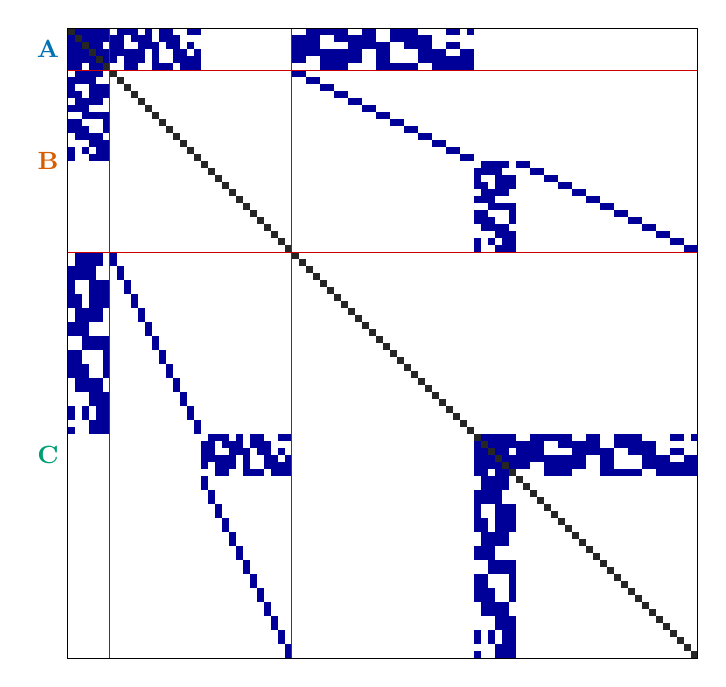
\begin{tikzpicture}[scale=1.0]
  \fill[black!85] (0.000,0.000) rectangle (0.089,-0.089);
  \fill[blue!60!black] (0.089,0.000) rectangle (0.178,-0.089);
  \fill[blue!60!black] (0.178,0.000) rectangle (0.267,-0.089);
  \fill[blue!60!black] (0.267,0.000) rectangle (0.356,-0.089);
  \fill[blue!60!black] (0.356,0.000) rectangle (0.444,-0.089);
  \fill[blue!60!black] (0.444,0.000) rectangle (0.533,-0.089);
  \fill[blue!60!black] (0.622,0.000) rectangle (0.711,-0.089);
  \fill[blue!60!black] (0.711,0.000) rectangle (0.800,-0.089);
  \fill[blue!60!black] (0.800,0.000) rectangle (0.889,-0.089);
  \fill[blue!60!black] (0.978,0.000) rectangle (1.067,-0.089);
  \fill[blue!60!black] (1.156,0.000) rectangle (1.244,-0.089);
  \fill[blue!60!black] (1.244,0.000) rectangle (1.333,-0.089);
  \fill[blue!60!black] (1.511,0.000) rectangle (1.600,-0.089);
  \fill[blue!60!black] (1.600,0.000) rectangle (1.689,-0.089);
  \fill[blue!60!black] (3.022,0.000) rectangle (3.111,-0.089);
  \fill[blue!60!black] (3.111,0.000) rectangle (3.200,-0.089);
  \fill[blue!60!black] (3.200,0.000) rectangle (3.289,-0.089);
  \fill[blue!60!black] (3.289,0.000) rectangle (3.378,-0.089);
  \fill[blue!60!black] (3.378,0.000) rectangle (3.467,-0.089);
  \fill[blue!60!black] (3.467,0.000) rectangle (3.556,-0.089);
  \fill[blue!60!black] (3.733,0.000) rectangle (3.822,-0.089);
  \fill[blue!60!black] (3.822,0.000) rectangle (3.911,-0.089);
  \fill[blue!60!black] (4.089,0.000) rectangle (4.178,-0.089);
  \fill[blue!60!black] (4.178,0.000) rectangle (4.267,-0.089);
  \fill[blue!60!black] (4.267,0.000) rectangle (4.356,-0.089);
  \fill[blue!60!black] (4.356,0.000) rectangle (4.444,-0.089);
  \fill[blue!60!black] (4.800,0.000) rectangle (4.889,-0.089);
  \fill[blue!60!black] (4.889,0.000) rectangle (4.978,-0.089);
  \fill[blue!60!black] (5.067,0.000) rectangle (5.156,-0.089);
  \fill[blue!60!black] (0.000,-0.089) rectangle (0.089,-0.178);
  \fill[black!85] (0.089,-0.089) rectangle (0.178,-0.178);
  \fill[blue!60!black] (0.178,-0.089) rectangle (0.267,-0.178);
  \fill[blue!60!black] (0.267,-0.089) rectangle (0.356,-0.178);
  \fill[blue!60!black] (0.356,-0.089) rectangle (0.444,-0.178);
  \fill[blue!60!black] (0.444,-0.089) rectangle (0.533,-0.178);
  \fill[blue!60!black] (0.533,-0.089) rectangle (0.622,-0.178);
  \fill[blue!60!black] (0.622,-0.089) rectangle (0.711,-0.178);
  \fill[blue!60!black] (0.800,-0.089) rectangle (0.889,-0.178);
  \fill[blue!60!black] (0.889,-0.089) rectangle (0.978,-0.178);
  \fill[blue!60!black] (0.978,-0.089) rectangle (1.067,-0.178);
  \fill[blue!60!black] (1.156,-0.089) rectangle (1.244,-0.178);
  \fill[blue!60!black] (1.244,-0.089) rectangle (1.333,-0.178);
  \fill[blue!60!black] (1.333,-0.089) rectangle (1.422,-0.178);
  \fill[blue!60!black] (2.844,-0.089) rectangle (2.933,-0.178);
  \fill[blue!60!black] (2.933,-0.089) rectangle (3.022,-0.178);
  \fill[blue!60!black] (3.022,-0.089) rectangle (3.111,-0.178);
  \fill[blue!60!black] (3.111,-0.089) rectangle (3.200,-0.178);
  \fill[blue!60!black] (3.378,-0.089) rectangle (3.467,-0.178);
  \fill[blue!60!black] (3.467,-0.089) rectangle (3.556,-0.178);
  \fill[blue!60!black] (3.556,-0.089) rectangle (3.644,-0.178);
  \fill[blue!60!black] (3.644,-0.089) rectangle (3.733,-0.178);
  \fill[blue!60!black] (3.733,-0.089) rectangle (3.822,-0.178);
  \fill[blue!60!black] (3.822,-0.089) rectangle (3.911,-0.178);
  \fill[blue!60!black] (4.089,-0.089) rectangle (4.178,-0.178);
  \fill[blue!60!black] (4.178,-0.089) rectangle (4.267,-0.178);
  \fill[blue!60!black] (4.267,-0.089) rectangle (4.356,-0.178);
  \fill[blue!60!black] (4.356,-0.089) rectangle (4.444,-0.178);
  \fill[blue!60!black] (4.444,-0.089) rectangle (4.533,-0.178);
  \fill[blue!60!black] (4.533,-0.089) rectangle (4.622,-0.178);
  \fill[blue!60!black] (0.000,-0.178) rectangle (0.089,-0.267);
  \fill[blue!60!black] (0.089,-0.178) rectangle (0.178,-0.267);
  \fill[black!85] (0.178,-0.178) rectangle (0.267,-0.267);
  \fill[blue!60!black] (0.267,-0.178) rectangle (0.356,-0.267);
  \fill[blue!60!black] (0.356,-0.178) rectangle (0.444,-0.267);
  \fill[blue!60!black] (0.533,-0.178) rectangle (0.622,-0.267);
  \fill[blue!60!black] (0.622,-0.178) rectangle (0.711,-0.267);
  \fill[blue!60!black] (0.889,-0.178) rectangle (0.978,-0.267);
  \fill[blue!60!black] (0.978,-0.178) rectangle (1.067,-0.267);
  \fill[blue!60!black] (1.067,-0.178) rectangle (1.156,-0.267);
  \fill[blue!60!black] (1.244,-0.178) rectangle (1.333,-0.267);
  \fill[blue!60!black] (1.333,-0.178) rectangle (1.422,-0.267);
  \fill[blue!60!black] (1.511,-0.178) rectangle (1.600,-0.267);
  \fill[blue!60!black] (2.844,-0.178) rectangle (2.933,-0.267);
  \fill[blue!60!black] (2.933,-0.178) rectangle (3.022,-0.267);
  \fill[blue!60!black] (3.022,-0.178) rectangle (3.111,-0.267);
  \fill[blue!60!black] (3.111,-0.178) rectangle (3.200,-0.267);
  \fill[blue!60!black] (3.556,-0.178) rectangle (3.644,-0.267);
  \fill[blue!60!black] (3.644,-0.178) rectangle (3.733,-0.267);
  \fill[blue!60!black] (3.733,-0.178) rectangle (3.822,-0.267);
  \fill[blue!60!black] (3.822,-0.178) rectangle (3.911,-0.267);
  \fill[blue!60!black] (3.911,-0.178) rectangle (4.000,-0.267);
  \fill[blue!60!black] (4.000,-0.178) rectangle (4.089,-0.267);
  \fill[blue!60!black] (4.267,-0.178) rectangle (4.356,-0.267);
  \fill[blue!60!black] (4.356,-0.178) rectangle (4.444,-0.267);
  \fill[blue!60!black] (4.444,-0.178) rectangle (4.533,-0.267);
  \fill[blue!60!black] (4.533,-0.178) rectangle (4.622,-0.267);
  \fill[blue!60!black] (4.800,-0.178) rectangle (4.889,-0.267);
  \fill[blue!60!black] (4.889,-0.178) rectangle (4.978,-0.267);
  \fill[blue!60!black] (0.000,-0.267) rectangle (0.089,-0.356);
  \fill[blue!60!black] (0.089,-0.267) rectangle (0.178,-0.356);
  \fill[blue!60!black] (0.178,-0.267) rectangle (0.267,-0.356);
  \fill[black!85] (0.267,-0.267) rectangle (0.356,-0.356);
  \fill[blue!60!black] (0.356,-0.267) rectangle (0.444,-0.356);
  \fill[blue!60!black] (0.444,-0.267) rectangle (0.533,-0.356);
  \fill[blue!60!black] (0.533,-0.267) rectangle (0.622,-0.356);
  \fill[blue!60!black] (0.622,-0.267) rectangle (0.711,-0.356);
  \fill[blue!60!black] (0.711,-0.267) rectangle (0.800,-0.356);
  \fill[blue!60!black] (0.800,-0.267) rectangle (0.889,-0.356);
  \fill[blue!60!black] (0.889,-0.267) rectangle (0.978,-0.356);
  \fill[blue!60!black] (1.067,-0.267) rectangle (1.156,-0.356);
  \fill[blue!60!black] (1.333,-0.267) rectangle (1.422,-0.356);
  \fill[blue!60!black] (1.422,-0.267) rectangle (1.511,-0.356);
  \fill[blue!60!black] (1.600,-0.267) rectangle (1.689,-0.356);
  \fill[blue!60!black] (2.844,-0.267) rectangle (2.933,-0.356);
  \fill[blue!60!black] (2.933,-0.267) rectangle (3.022,-0.356);
  \fill[blue!60!black] (3.022,-0.267) rectangle (3.111,-0.356);
  \fill[blue!60!black] (3.111,-0.267) rectangle (3.200,-0.356);
  \fill[blue!60!black] (3.200,-0.267) rectangle (3.289,-0.356);
  \fill[blue!60!black] (3.289,-0.267) rectangle (3.378,-0.356);
  \fill[blue!60!black] (3.378,-0.267) rectangle (3.467,-0.356);
  \fill[blue!60!black] (3.467,-0.267) rectangle (3.556,-0.356);
  \fill[blue!60!black] (3.556,-0.267) rectangle (3.644,-0.356);
  \fill[blue!60!black] (3.644,-0.267) rectangle (3.733,-0.356);
  \fill[blue!60!black] (3.911,-0.267) rectangle (4.000,-0.356);
  \fill[blue!60!black] (4.000,-0.267) rectangle (4.089,-0.356);
  \fill[blue!60!black] (4.444,-0.267) rectangle (4.533,-0.356);
  \fill[blue!60!black] (4.533,-0.267) rectangle (4.622,-0.356);
  \fill[blue!60!black] (4.622,-0.267) rectangle (4.711,-0.356);
  \fill[blue!60!black] (4.711,-0.267) rectangle (4.800,-0.356);
  \fill[blue!60!black] (4.978,-0.267) rectangle (5.067,-0.356);
  \fill[blue!60!black] (5.067,-0.267) rectangle (5.156,-0.356);
  \fill[blue!60!black] (0.000,-0.356) rectangle (0.089,-0.444);
  \fill[blue!60!black] (0.089,-0.356) rectangle (0.178,-0.444);
  \fill[blue!60!black] (0.178,-0.356) rectangle (0.267,-0.444);
  \fill[blue!60!black] (0.267,-0.356) rectangle (0.356,-0.444);
  \fill[black!85] (0.356,-0.356) rectangle (0.444,-0.444);
  \fill[blue!60!black] (0.444,-0.356) rectangle (0.533,-0.444);
  \fill[blue!60!black] (0.533,-0.356) rectangle (0.622,-0.444);
  \fill[blue!60!black] (0.711,-0.356) rectangle (0.800,-0.444);
  \fill[blue!60!black] (0.800,-0.356) rectangle (0.889,-0.444);
  \fill[blue!60!black] (0.889,-0.356) rectangle (0.978,-0.444);
  \fill[blue!60!black] (1.067,-0.356) rectangle (1.156,-0.444);
  \fill[blue!60!black] (1.333,-0.356) rectangle (1.422,-0.444);
  \fill[blue!60!black] (1.422,-0.356) rectangle (1.511,-0.444);
  \fill[blue!60!black] (1.511,-0.356) rectangle (1.600,-0.444);
  \fill[blue!60!black] (1.600,-0.356) rectangle (1.689,-0.444);
  \fill[blue!60!black] (2.844,-0.356) rectangle (2.933,-0.444);
  \fill[blue!60!black] (2.933,-0.356) rectangle (3.022,-0.444);
  \fill[blue!60!black] (3.200,-0.356) rectangle (3.289,-0.444);
  \fill[blue!60!black] (3.289,-0.356) rectangle (3.378,-0.444);
  \fill[blue!60!black] (3.378,-0.356) rectangle (3.467,-0.444);
  \fill[blue!60!black] (3.467,-0.356) rectangle (3.556,-0.444);
  \fill[blue!60!black] (3.556,-0.356) rectangle (3.644,-0.444);
  \fill[blue!60!black] (3.644,-0.356) rectangle (3.733,-0.444);
  \fill[blue!60!black] (3.911,-0.356) rectangle (4.000,-0.444);
  \fill[blue!60!black] (4.000,-0.356) rectangle (4.089,-0.444);
  \fill[blue!60!black] (4.444,-0.356) rectangle (4.533,-0.444);
  \fill[blue!60!black] (4.533,-0.356) rectangle (4.622,-0.444);
  \fill[blue!60!black] (4.622,-0.356) rectangle (4.711,-0.444);
  \fill[blue!60!black] (4.711,-0.356) rectangle (4.800,-0.444);
  \fill[blue!60!black] (4.800,-0.356) rectangle (4.889,-0.444);
  \fill[blue!60!black] (4.889,-0.356) rectangle (4.978,-0.444);
  \fill[blue!60!black] (4.978,-0.356) rectangle (5.067,-0.444);
  \fill[blue!60!black] (5.067,-0.356) rectangle (5.156,-0.444);
  \fill[blue!60!black] (0.000,-0.444) rectangle (0.089,-0.533);
  \fill[blue!60!black] (0.089,-0.444) rectangle (0.178,-0.533);
  \fill[blue!60!black] (0.267,-0.444) rectangle (0.356,-0.533);
  \fill[blue!60!black] (0.356,-0.444) rectangle (0.444,-0.533);
  \fill[black!85] (0.444,-0.444) rectangle (0.533,-0.533);
  \fill[blue!60!black] (0.711,-0.444) rectangle (0.800,-0.533);
  \fill[blue!60!black] (0.800,-0.444) rectangle (0.889,-0.533);
  \fill[blue!60!black] (1.067,-0.444) rectangle (1.156,-0.533);
  \fill[blue!60!black] (1.156,-0.444) rectangle (1.244,-0.533);
  \fill[blue!60!black] (1.244,-0.444) rectangle (1.333,-0.533);
  \fill[blue!60!black] (1.422,-0.444) rectangle (1.511,-0.533);
  \fill[blue!60!black] (1.511,-0.444) rectangle (1.600,-0.533);
  \fill[blue!60!black] (1.600,-0.444) rectangle (1.689,-0.533);
  \fill[blue!60!black] (3.200,-0.444) rectangle (3.289,-0.533);
  \fill[blue!60!black] (3.289,-0.444) rectangle (3.378,-0.533);
  \fill[blue!60!black] (3.378,-0.444) rectangle (3.467,-0.533);
  \fill[blue!60!black] (3.467,-0.444) rectangle (3.556,-0.533);
  \fill[blue!60!black] (3.911,-0.444) rectangle (4.000,-0.533);
  \fill[blue!60!black] (4.000,-0.444) rectangle (4.089,-0.533);
  \fill[blue!60!black] (4.089,-0.444) rectangle (4.178,-0.533);
  \fill[blue!60!black] (4.178,-0.444) rectangle (4.267,-0.533);
  \fill[blue!60!black] (4.267,-0.444) rectangle (4.356,-0.533);
  \fill[blue!60!black] (4.356,-0.444) rectangle (4.444,-0.533);
  \fill[blue!60!black] (4.622,-0.444) rectangle (4.711,-0.533);
  \fill[blue!60!black] (4.711,-0.444) rectangle (4.800,-0.533);
  \fill[blue!60!black] (4.800,-0.444) rectangle (4.889,-0.533);
  \fill[blue!60!black] (4.889,-0.444) rectangle (4.978,-0.533);
  \fill[blue!60!black] (4.978,-0.444) rectangle (5.067,-0.533);
  \fill[blue!60!black] (5.067,-0.444) rectangle (5.156,-0.533);
  \fill[blue!60!black] (0.089,-0.533) rectangle (0.178,-0.622);
  \fill[blue!60!black] (0.178,-0.533) rectangle (0.267,-0.622);
  \fill[blue!60!black] (0.267,-0.533) rectangle (0.356,-0.622);
  \fill[blue!60!black] (0.356,-0.533) rectangle (0.444,-0.622);
  \fill[black!85] (0.533,-0.533) rectangle (0.622,-0.622);
  \fill[blue!60!black] (2.844,-0.533) rectangle (2.933,-0.622);
  \fill[blue!60!black] (2.933,-0.533) rectangle (3.022,-0.622);
  \fill[blue!60!black] (0.000,-0.622) rectangle (0.089,-0.711);
  \fill[blue!60!black] (0.089,-0.622) rectangle (0.178,-0.711);
  \fill[blue!60!black] (0.178,-0.622) rectangle (0.267,-0.711);
  \fill[blue!60!black] (0.267,-0.622) rectangle (0.356,-0.711);
  \fill[black!85] (0.622,-0.622) rectangle (0.711,-0.711);
  \fill[blue!60!black] (3.022,-0.622) rectangle (3.111,-0.711);
  \fill[blue!60!black] (3.111,-0.622) rectangle (3.200,-0.711);
  \fill[blue!60!black] (0.000,-0.711) rectangle (0.089,-0.800);
  \fill[blue!60!black] (0.267,-0.711) rectangle (0.356,-0.800);
  \fill[blue!60!black] (0.356,-0.711) rectangle (0.444,-0.800);
  \fill[blue!60!black] (0.444,-0.711) rectangle (0.533,-0.800);
  \fill[black!85] (0.711,-0.711) rectangle (0.800,-0.800);
  \fill[blue!60!black] (3.200,-0.711) rectangle (3.289,-0.800);
  \fill[blue!60!black] (3.289,-0.711) rectangle (3.378,-0.800);
  \fill[blue!60!black] (0.000,-0.800) rectangle (0.089,-0.889);
  \fill[blue!60!black] (0.089,-0.800) rectangle (0.178,-0.889);
  \fill[blue!60!black] (0.267,-0.800) rectangle (0.356,-0.889);
  \fill[blue!60!black] (0.356,-0.800) rectangle (0.444,-0.889);
  \fill[blue!60!black] (0.444,-0.800) rectangle (0.533,-0.889);
  \fill[black!85] (0.800,-0.800) rectangle (0.889,-0.889);
  \fill[blue!60!black] (3.378,-0.800) rectangle (3.467,-0.889);
  \fill[blue!60!black] (3.467,-0.800) rectangle (3.556,-0.889);
  \fill[blue!60!black] (0.089,-0.889) rectangle (0.178,-0.978);
  \fill[blue!60!black] (0.178,-0.889) rectangle (0.267,-0.978);
  \fill[blue!60!black] (0.267,-0.889) rectangle (0.356,-0.978);
  \fill[blue!60!black] (0.356,-0.889) rectangle (0.444,-0.978);
  \fill[black!85] (0.889,-0.889) rectangle (0.978,-0.978);
  \fill[blue!60!black] (3.556,-0.889) rectangle (3.644,-0.978);
  \fill[blue!60!black] (3.644,-0.889) rectangle (3.733,-0.978);
  \fill[blue!60!black] (0.000,-0.978) rectangle (0.089,-1.067);
  \fill[blue!60!black] (0.089,-0.978) rectangle (0.178,-1.067);
  \fill[blue!60!black] (0.178,-0.978) rectangle (0.267,-1.067);
  \fill[black!85] (0.978,-0.978) rectangle (1.067,-1.067);
  \fill[blue!60!black] (3.733,-0.978) rectangle (3.822,-1.067);
  \fill[blue!60!black] (3.822,-0.978) rectangle (3.911,-1.067);
  \fill[blue!60!black] (0.178,-1.067) rectangle (0.267,-1.156);
  \fill[blue!60!black] (0.267,-1.067) rectangle (0.356,-1.156);
  \fill[blue!60!black] (0.356,-1.067) rectangle (0.444,-1.156);
  \fill[blue!60!black] (0.444,-1.067) rectangle (0.533,-1.156);
  \fill[black!85] (1.067,-1.067) rectangle (1.156,-1.156);
  \fill[blue!60!black] (3.911,-1.067) rectangle (4.000,-1.156);
  \fill[blue!60!black] (4.000,-1.067) rectangle (4.089,-1.156);
  \fill[blue!60!black] (0.000,-1.156) rectangle (0.089,-1.244);
  \fill[blue!60!black] (0.089,-1.156) rectangle (0.178,-1.244);
  \fill[blue!60!black] (0.444,-1.156) rectangle (0.533,-1.244);
  \fill[black!85] (1.156,-1.156) rectangle (1.244,-1.244);
  \fill[blue!60!black] (4.089,-1.156) rectangle (4.178,-1.244);
  \fill[blue!60!black] (4.178,-1.156) rectangle (4.267,-1.244);
  \fill[blue!60!black] (0.000,-1.244) rectangle (0.089,-1.333);
  \fill[blue!60!black] (0.089,-1.244) rectangle (0.178,-1.333);
  \fill[blue!60!black] (0.178,-1.244) rectangle (0.267,-1.333);
  \fill[blue!60!black] (0.444,-1.244) rectangle (0.533,-1.333);
  \fill[black!85] (1.244,-1.244) rectangle (1.333,-1.333);
  \fill[blue!60!black] (4.267,-1.244) rectangle (4.356,-1.333);
  \fill[blue!60!black] (4.356,-1.244) rectangle (4.444,-1.333);
  \fill[blue!60!black] (0.089,-1.333) rectangle (0.178,-1.422);
  \fill[blue!60!black] (0.178,-1.333) rectangle (0.267,-1.422);
  \fill[blue!60!black] (0.267,-1.333) rectangle (0.356,-1.422);
  \fill[blue!60!black] (0.356,-1.333) rectangle (0.444,-1.422);
  \fill[black!85] (1.333,-1.333) rectangle (1.422,-1.422);
  \fill[blue!60!black] (4.444,-1.333) rectangle (4.533,-1.422);
  \fill[blue!60!black] (4.533,-1.333) rectangle (4.622,-1.422);
  \fill[blue!60!black] (0.267,-1.422) rectangle (0.356,-1.511);
  \fill[blue!60!black] (0.356,-1.422) rectangle (0.444,-1.511);
  \fill[blue!60!black] (0.444,-1.422) rectangle (0.533,-1.511);
  \fill[black!85] (1.422,-1.422) rectangle (1.511,-1.511);
  \fill[blue!60!black] (4.622,-1.422) rectangle (4.711,-1.511);
  \fill[blue!60!black] (4.711,-1.422) rectangle (4.800,-1.511);
  \fill[blue!60!black] (0.000,-1.511) rectangle (0.089,-1.600);
  \fill[blue!60!black] (0.178,-1.511) rectangle (0.267,-1.600);
  \fill[blue!60!black] (0.356,-1.511) rectangle (0.444,-1.600);
  \fill[blue!60!black] (0.444,-1.511) rectangle (0.533,-1.600);
  \fill[black!85] (1.511,-1.511) rectangle (1.600,-1.600);
  \fill[blue!60!black] (4.800,-1.511) rectangle (4.889,-1.600);
  \fill[blue!60!black] (4.889,-1.511) rectangle (4.978,-1.600);
  \fill[blue!60!black] (0.000,-1.600) rectangle (0.089,-1.689);
  \fill[blue!60!black] (0.267,-1.600) rectangle (0.356,-1.689);
  \fill[blue!60!black] (0.356,-1.600) rectangle (0.444,-1.689);
  \fill[blue!60!black] (0.444,-1.600) rectangle (0.533,-1.689);
  \fill[black!85] (1.600,-1.600) rectangle (1.689,-1.689);
  \fill[blue!60!black] (4.978,-1.600) rectangle (5.067,-1.689);
  \fill[blue!60!black] (5.067,-1.600) rectangle (5.156,-1.689);
  \fill[black!85] (1.689,-1.689) rectangle (1.778,-1.778);
  \fill[blue!60!black] (5.244,-1.689) rectangle (5.333,-1.778);
  \fill[blue!60!black] (5.333,-1.689) rectangle (5.422,-1.778);
  \fill[blue!60!black] (5.422,-1.689) rectangle (5.511,-1.778);
  \fill[blue!60!black] (5.511,-1.689) rectangle (5.600,-1.778);
  \fill[blue!60!black] (5.689,-1.689) rectangle (5.778,-1.778);
  \fill[blue!60!black] (5.778,-1.689) rectangle (5.867,-1.778);
  \fill[black!85] (1.778,-1.778) rectangle (1.867,-1.867);
  \fill[blue!60!black] (5.156,-1.778) rectangle (5.244,-1.867);
  \fill[blue!60!black] (5.244,-1.778) rectangle (5.333,-1.867);
  \fill[blue!60!black] (5.333,-1.778) rectangle (5.422,-1.867);
  \fill[blue!60!black] (5.422,-1.778) rectangle (5.511,-1.867);
  \fill[blue!60!black] (5.867,-1.778) rectangle (5.956,-1.867);
  \fill[blue!60!black] (5.956,-1.778) rectangle (6.044,-1.867);
  \fill[black!85] (1.867,-1.867) rectangle (1.956,-1.956);
  \fill[blue!60!black] (5.156,-1.867) rectangle (5.244,-1.956);
  \fill[blue!60!black] (5.422,-1.867) rectangle (5.511,-1.956);
  \fill[blue!60!black] (5.511,-1.867) rectangle (5.600,-1.956);
  \fill[blue!60!black] (5.600,-1.867) rectangle (5.689,-1.956);
  \fill[blue!60!black] (6.044,-1.867) rectangle (6.133,-1.956);
  \fill[blue!60!black] (6.133,-1.867) rectangle (6.222,-1.956);
  \fill[black!85] (1.956,-1.956) rectangle (2.044,-2.044);
  \fill[blue!60!black] (5.156,-1.956) rectangle (5.244,-2.044);
  \fill[blue!60!black] (5.244,-1.956) rectangle (5.333,-2.044);
  \fill[blue!60!black] (5.422,-1.956) rectangle (5.511,-2.044);
  \fill[blue!60!black] (5.511,-1.956) rectangle (5.600,-2.044);
  \fill[blue!60!black] (5.600,-1.956) rectangle (5.689,-2.044);
  \fill[blue!60!black] (6.222,-1.956) rectangle (6.311,-2.044);
  \fill[blue!60!black] (6.311,-1.956) rectangle (6.400,-2.044);
  \fill[black!85] (2.044,-2.044) rectangle (2.133,-2.133);
  \fill[blue!60!black] (5.244,-2.044) rectangle (5.333,-2.133);
  \fill[blue!60!black] (5.333,-2.044) rectangle (5.422,-2.133);
  \fill[blue!60!black] (5.422,-2.044) rectangle (5.511,-2.133);
  \fill[blue!60!black] (5.511,-2.044) rectangle (5.600,-2.133);
  \fill[blue!60!black] (6.400,-2.044) rectangle (6.489,-2.133);
  \fill[blue!60!black] (6.489,-2.044) rectangle (6.578,-2.133);
  \fill[black!85] (2.133,-2.133) rectangle (2.222,-2.222);
  \fill[blue!60!black] (5.156,-2.133) rectangle (5.244,-2.222);
  \fill[blue!60!black] (5.244,-2.133) rectangle (5.333,-2.222);
  \fill[blue!60!black] (5.333,-2.133) rectangle (5.422,-2.222);
  \fill[blue!60!black] (6.578,-2.133) rectangle (6.667,-2.222);
  \fill[blue!60!black] (6.667,-2.133) rectangle (6.756,-2.222);
  \fill[black!85] (2.222,-2.222) rectangle (2.311,-2.311);
  \fill[blue!60!black] (5.333,-2.222) rectangle (5.422,-2.311);
  \fill[blue!60!black] (5.422,-2.222) rectangle (5.511,-2.311);
  \fill[blue!60!black] (5.511,-2.222) rectangle (5.600,-2.311);
  \fill[blue!60!black] (5.600,-2.222) rectangle (5.689,-2.311);
  \fill[blue!60!black] (6.756,-2.222) rectangle (6.844,-2.311);
  \fill[blue!60!black] (6.844,-2.222) rectangle (6.933,-2.311);
  \fill[black!85] (2.311,-2.311) rectangle (2.400,-2.400);
  \fill[blue!60!black] (5.156,-2.311) rectangle (5.244,-2.400);
  \fill[blue!60!black] (5.244,-2.311) rectangle (5.333,-2.400);
  \fill[blue!60!black] (5.600,-2.311) rectangle (5.689,-2.400);
  \fill[blue!60!black] (6.933,-2.311) rectangle (7.022,-2.400);
  \fill[blue!60!black] (7.022,-2.311) rectangle (7.111,-2.400);
  \fill[black!85] (2.400,-2.400) rectangle (2.489,-2.489);
  \fill[blue!60!black] (5.156,-2.400) rectangle (5.244,-2.489);
  \fill[blue!60!black] (5.244,-2.400) rectangle (5.333,-2.489);
  \fill[blue!60!black] (5.333,-2.400) rectangle (5.422,-2.489);
  \fill[blue!60!black] (5.600,-2.400) rectangle (5.689,-2.489);
  \fill[blue!60!black] (7.111,-2.400) rectangle (7.200,-2.489);
  \fill[blue!60!black] (7.200,-2.400) rectangle (7.289,-2.489);
  \fill[black!85] (2.489,-2.489) rectangle (2.578,-2.578);
  \fill[blue!60!black] (5.244,-2.489) rectangle (5.333,-2.578);
  \fill[blue!60!black] (5.333,-2.489) rectangle (5.422,-2.578);
  \fill[blue!60!black] (5.422,-2.489) rectangle (5.511,-2.578);
  \fill[blue!60!black] (5.511,-2.489) rectangle (5.600,-2.578);
  \fill[blue!60!black] (7.289,-2.489) rectangle (7.378,-2.578);
  \fill[blue!60!black] (7.378,-2.489) rectangle (7.467,-2.578);
  \fill[black!85] (2.578,-2.578) rectangle (2.667,-2.667);
  \fill[blue!60!black] (5.422,-2.578) rectangle (5.511,-2.667);
  \fill[blue!60!black] (5.511,-2.578) rectangle (5.600,-2.667);
  \fill[blue!60!black] (5.600,-2.578) rectangle (5.689,-2.667);
  \fill[blue!60!black] (7.467,-2.578) rectangle (7.556,-2.667);
  \fill[blue!60!black] (7.556,-2.578) rectangle (7.644,-2.667);
  \fill[black!85] (2.667,-2.667) rectangle (2.756,-2.756);
  \fill[blue!60!black] (5.156,-2.667) rectangle (5.244,-2.756);
  \fill[blue!60!black] (5.333,-2.667) rectangle (5.422,-2.756);
  \fill[blue!60!black] (5.511,-2.667) rectangle (5.600,-2.756);
  \fill[blue!60!black] (5.600,-2.667) rectangle (5.689,-2.756);
  \fill[blue!60!black] (7.644,-2.667) rectangle (7.733,-2.756);
  \fill[blue!60!black] (7.733,-2.667) rectangle (7.822,-2.756);
  \fill[black!85] (2.756,-2.756) rectangle (2.844,-2.844);
  \fill[blue!60!black] (5.156,-2.756) rectangle (5.244,-2.844);
  \fill[blue!60!black] (5.422,-2.756) rectangle (5.511,-2.844);
  \fill[blue!60!black] (5.511,-2.756) rectangle (5.600,-2.844);
  \fill[blue!60!black] (5.600,-2.756) rectangle (5.689,-2.844);
  \fill[blue!60!black] (7.822,-2.756) rectangle (7.911,-2.844);
  \fill[blue!60!black] (7.911,-2.756) rectangle (8.000,-2.844);
  \fill[blue!60!black] (0.089,-2.844) rectangle (0.178,-2.933);
  \fill[blue!60!black] (0.178,-2.844) rectangle (0.267,-2.933);
  \fill[blue!60!black] (0.267,-2.844) rectangle (0.356,-2.933);
  \fill[blue!60!black] (0.356,-2.844) rectangle (0.444,-2.933);
  \fill[blue!60!black] (0.533,-2.844) rectangle (0.622,-2.933);
  \fill[black!85] (2.844,-2.844) rectangle (2.933,-2.933);
  \fill[blue!60!black] (0.089,-2.933) rectangle (0.178,-3.022);
  \fill[blue!60!black] (0.178,-2.933) rectangle (0.267,-3.022);
  \fill[blue!60!black] (0.267,-2.933) rectangle (0.356,-3.022);
  \fill[blue!60!black] (0.356,-2.933) rectangle (0.444,-3.022);
  \fill[blue!60!black] (0.533,-2.933) rectangle (0.622,-3.022);
  \fill[black!85] (2.933,-2.933) rectangle (3.022,-3.022);
  \fill[blue!60!black] (0.000,-3.022) rectangle (0.089,-3.111);
  \fill[blue!60!black] (0.089,-3.022) rectangle (0.178,-3.111);
  \fill[blue!60!black] (0.178,-3.022) rectangle (0.267,-3.111);
  \fill[blue!60!black] (0.267,-3.022) rectangle (0.356,-3.111);
  \fill[blue!60!black] (0.622,-3.022) rectangle (0.711,-3.111);
  \fill[black!85] (3.022,-3.022) rectangle (3.111,-3.111);
  \fill[blue!60!black] (0.000,-3.111) rectangle (0.089,-3.200);
  \fill[blue!60!black] (0.089,-3.111) rectangle (0.178,-3.200);
  \fill[blue!60!black] (0.178,-3.111) rectangle (0.267,-3.200);
  \fill[blue!60!black] (0.267,-3.111) rectangle (0.356,-3.200);
  \fill[blue!60!black] (0.622,-3.111) rectangle (0.711,-3.200);
  \fill[black!85] (3.111,-3.111) rectangle (3.200,-3.200);
  \fill[blue!60!black] (0.000,-3.200) rectangle (0.089,-3.289);
  \fill[blue!60!black] (0.267,-3.200) rectangle (0.356,-3.289);
  \fill[blue!60!black] (0.356,-3.200) rectangle (0.444,-3.289);
  \fill[blue!60!black] (0.444,-3.200) rectangle (0.533,-3.289);
  \fill[blue!60!black] (0.711,-3.200) rectangle (0.800,-3.289);
  \fill[black!85] (3.200,-3.200) rectangle (3.289,-3.289);
  \fill[blue!60!black] (0.000,-3.289) rectangle (0.089,-3.378);
  \fill[blue!60!black] (0.267,-3.289) rectangle (0.356,-3.378);
  \fill[blue!60!black] (0.356,-3.289) rectangle (0.444,-3.378);
  \fill[blue!60!black] (0.444,-3.289) rectangle (0.533,-3.378);
  \fill[blue!60!black] (0.711,-3.289) rectangle (0.800,-3.378);
  \fill[black!85] (3.289,-3.289) rectangle (3.378,-3.378);
  \fill[blue!60!black] (0.000,-3.378) rectangle (0.089,-3.467);
  \fill[blue!60!black] (0.089,-3.378) rectangle (0.178,-3.467);
  \fill[blue!60!black] (0.267,-3.378) rectangle (0.356,-3.467);
  \fill[blue!60!black] (0.356,-3.378) rectangle (0.444,-3.467);
  \fill[blue!60!black] (0.444,-3.378) rectangle (0.533,-3.467);
  \fill[blue!60!black] (0.800,-3.378) rectangle (0.889,-3.467);
  \fill[black!85] (3.378,-3.378) rectangle (3.467,-3.467);
  \fill[blue!60!black] (0.000,-3.467) rectangle (0.089,-3.556);
  \fill[blue!60!black] (0.089,-3.467) rectangle (0.178,-3.556);
  \fill[blue!60!black] (0.267,-3.467) rectangle (0.356,-3.556);
  \fill[blue!60!black] (0.356,-3.467) rectangle (0.444,-3.556);
  \fill[blue!60!black] (0.444,-3.467) rectangle (0.533,-3.556);
  \fill[blue!60!black] (0.800,-3.467) rectangle (0.889,-3.556);
  \fill[black!85] (3.467,-3.467) rectangle (3.556,-3.556);
  \fill[blue!60!black] (0.089,-3.556) rectangle (0.178,-3.644);
  \fill[blue!60!black] (0.178,-3.556) rectangle (0.267,-3.644);
  \fill[blue!60!black] (0.267,-3.556) rectangle (0.356,-3.644);
  \fill[blue!60!black] (0.356,-3.556) rectangle (0.444,-3.644);
  \fill[blue!60!black] (0.889,-3.556) rectangle (0.978,-3.644);
  \fill[black!85] (3.556,-3.556) rectangle (3.644,-3.644);
  \fill[blue!60!black] (0.089,-3.644) rectangle (0.178,-3.733);
  \fill[blue!60!black] (0.178,-3.644) rectangle (0.267,-3.733);
  \fill[blue!60!black] (0.267,-3.644) rectangle (0.356,-3.733);
  \fill[blue!60!black] (0.356,-3.644) rectangle (0.444,-3.733);
  \fill[blue!60!black] (0.889,-3.644) rectangle (0.978,-3.733);
  \fill[black!85] (3.644,-3.644) rectangle (3.733,-3.733);
  \fill[blue!60!black] (0.000,-3.733) rectangle (0.089,-3.822);
  \fill[blue!60!black] (0.089,-3.733) rectangle (0.178,-3.822);
  \fill[blue!60!black] (0.178,-3.733) rectangle (0.267,-3.822);
  \fill[blue!60!black] (0.978,-3.733) rectangle (1.067,-3.822);
  \fill[black!85] (3.733,-3.733) rectangle (3.822,-3.822);
  \fill[blue!60!black] (0.000,-3.822) rectangle (0.089,-3.911);
  \fill[blue!60!black] (0.089,-3.822) rectangle (0.178,-3.911);
  \fill[blue!60!black] (0.178,-3.822) rectangle (0.267,-3.911);
  \fill[blue!60!black] (0.978,-3.822) rectangle (1.067,-3.911);
  \fill[black!85] (3.822,-3.822) rectangle (3.911,-3.911);
  \fill[blue!60!black] (0.178,-3.911) rectangle (0.267,-4.000);
  \fill[blue!60!black] (0.267,-3.911) rectangle (0.356,-4.000);
  \fill[blue!60!black] (0.356,-3.911) rectangle (0.444,-4.000);
  \fill[blue!60!black] (0.444,-3.911) rectangle (0.533,-4.000);
  \fill[blue!60!black] (1.067,-3.911) rectangle (1.156,-4.000);
  \fill[black!85] (3.911,-3.911) rectangle (4.000,-4.000);
  \fill[blue!60!black] (0.178,-4.000) rectangle (0.267,-4.089);
  \fill[blue!60!black] (0.267,-4.000) rectangle (0.356,-4.089);
  \fill[blue!60!black] (0.356,-4.000) rectangle (0.444,-4.089);
  \fill[blue!60!black] (0.444,-4.000) rectangle (0.533,-4.089);
  \fill[blue!60!black] (1.067,-4.000) rectangle (1.156,-4.089);
  \fill[black!85] (4.000,-4.000) rectangle (4.089,-4.089);
  \fill[blue!60!black] (0.000,-4.089) rectangle (0.089,-4.178);
  \fill[blue!60!black] (0.089,-4.089) rectangle (0.178,-4.178);
  \fill[blue!60!black] (0.444,-4.089) rectangle (0.533,-4.178);
  \fill[blue!60!black] (1.156,-4.089) rectangle (1.244,-4.178);
  \fill[black!85] (4.089,-4.089) rectangle (4.178,-4.178);
  \fill[blue!60!black] (0.000,-4.178) rectangle (0.089,-4.267);
  \fill[blue!60!black] (0.089,-4.178) rectangle (0.178,-4.267);
  \fill[blue!60!black] (0.444,-4.178) rectangle (0.533,-4.267);
  \fill[blue!60!black] (1.156,-4.178) rectangle (1.244,-4.267);
  \fill[black!85] (4.178,-4.178) rectangle (4.267,-4.267);
  \fill[blue!60!black] (0.000,-4.267) rectangle (0.089,-4.356);
  \fill[blue!60!black] (0.089,-4.267) rectangle (0.178,-4.356);
  \fill[blue!60!black] (0.178,-4.267) rectangle (0.267,-4.356);
  \fill[blue!60!black] (0.444,-4.267) rectangle (0.533,-4.356);
  \fill[blue!60!black] (1.244,-4.267) rectangle (1.333,-4.356);
  \fill[black!85] (4.267,-4.267) rectangle (4.356,-4.356);
  \fill[blue!60!black] (0.000,-4.356) rectangle (0.089,-4.444);
  \fill[blue!60!black] (0.089,-4.356) rectangle (0.178,-4.444);
  \fill[blue!60!black] (0.178,-4.356) rectangle (0.267,-4.444);
  \fill[blue!60!black] (0.444,-4.356) rectangle (0.533,-4.444);
  \fill[blue!60!black] (1.244,-4.356) rectangle (1.333,-4.444);
  \fill[black!85] (4.356,-4.356) rectangle (4.444,-4.444);
  \fill[blue!60!black] (0.089,-4.444) rectangle (0.178,-4.533);
  \fill[blue!60!black] (0.178,-4.444) rectangle (0.267,-4.533);
  \fill[blue!60!black] (0.267,-4.444) rectangle (0.356,-4.533);
  \fill[blue!60!black] (0.356,-4.444) rectangle (0.444,-4.533);
  \fill[blue!60!black] (1.333,-4.444) rectangle (1.422,-4.533);
  \fill[black!85] (4.444,-4.444) rectangle (4.533,-4.533);
  \fill[blue!60!black] (0.089,-4.533) rectangle (0.178,-4.622);
  \fill[blue!60!black] (0.178,-4.533) rectangle (0.267,-4.622);
  \fill[blue!60!black] (0.267,-4.533) rectangle (0.356,-4.622);
  \fill[blue!60!black] (0.356,-4.533) rectangle (0.444,-4.622);
  \fill[blue!60!black] (1.333,-4.533) rectangle (1.422,-4.622);
  \fill[black!85] (4.533,-4.533) rectangle (4.622,-4.622);
  \fill[blue!60!black] (0.267,-4.622) rectangle (0.356,-4.711);
  \fill[blue!60!black] (0.356,-4.622) rectangle (0.444,-4.711);
  \fill[blue!60!black] (0.444,-4.622) rectangle (0.533,-4.711);
  \fill[blue!60!black] (1.422,-4.622) rectangle (1.511,-4.711);
  \fill[black!85] (4.622,-4.622) rectangle (4.711,-4.711);
  \fill[blue!60!black] (0.267,-4.711) rectangle (0.356,-4.800);
  \fill[blue!60!black] (0.356,-4.711) rectangle (0.444,-4.800);
  \fill[blue!60!black] (0.444,-4.711) rectangle (0.533,-4.800);
  \fill[blue!60!black] (1.422,-4.711) rectangle (1.511,-4.800);
  \fill[black!85] (4.711,-4.711) rectangle (4.800,-4.800);
  \fill[blue!60!black] (0.000,-4.800) rectangle (0.089,-4.889);
  \fill[blue!60!black] (0.178,-4.800) rectangle (0.267,-4.889);
  \fill[blue!60!black] (0.356,-4.800) rectangle (0.444,-4.889);
  \fill[blue!60!black] (0.444,-4.800) rectangle (0.533,-4.889);
  \fill[blue!60!black] (1.511,-4.800) rectangle (1.600,-4.889);
  \fill[black!85] (4.800,-4.800) rectangle (4.889,-4.889);
  \fill[blue!60!black] (0.000,-4.889) rectangle (0.089,-4.978);
  \fill[blue!60!black] (0.178,-4.889) rectangle (0.267,-4.978);
  \fill[blue!60!black] (0.356,-4.889) rectangle (0.444,-4.978);
  \fill[blue!60!black] (0.444,-4.889) rectangle (0.533,-4.978);
  \fill[blue!60!black] (1.511,-4.889) rectangle (1.600,-4.978);
  \fill[black!85] (4.889,-4.889) rectangle (4.978,-4.978);
  \fill[blue!60!black] (0.267,-4.978) rectangle (0.356,-5.067);
  \fill[blue!60!black] (0.356,-4.978) rectangle (0.444,-5.067);
  \fill[blue!60!black] (0.444,-4.978) rectangle (0.533,-5.067);
  \fill[blue!60!black] (1.600,-4.978) rectangle (1.689,-5.067);
  \fill[black!85] (4.978,-4.978) rectangle (5.067,-5.067);
  \fill[blue!60!black] (0.000,-5.067) rectangle (0.089,-5.156);
  \fill[blue!60!black] (0.267,-5.067) rectangle (0.356,-5.156);
  \fill[blue!60!black] (0.356,-5.067) rectangle (0.444,-5.156);
  \fill[blue!60!black] (0.444,-5.067) rectangle (0.533,-5.156);
  \fill[blue!60!black] (1.600,-5.067) rectangle (1.689,-5.156);
  \fill[black!85] (5.067,-5.067) rectangle (5.156,-5.156);
  \fill[blue!60!black] (1.778,-5.156) rectangle (1.867,-5.244);
  \fill[blue!60!black] (1.867,-5.156) rectangle (1.956,-5.244);
  \fill[blue!60!black] (1.956,-5.156) rectangle (2.044,-5.244);
  \fill[blue!60!black] (2.133,-5.156) rectangle (2.222,-5.244);
  \fill[blue!60!black] (2.311,-5.156) rectangle (2.400,-5.244);
  \fill[blue!60!black] (2.400,-5.156) rectangle (2.489,-5.244);
  \fill[blue!60!black] (2.667,-5.156) rectangle (2.756,-5.244);
  \fill[blue!60!black] (2.756,-5.156) rectangle (2.844,-5.244);
  \fill[black!85] (5.156,-5.156) rectangle (5.244,-5.244);
  \fill[blue!60!black] (5.244,-5.156) rectangle (5.333,-5.244);
  \fill[blue!60!black] (5.333,-5.156) rectangle (5.422,-5.244);
  \fill[blue!60!black] (5.422,-5.156) rectangle (5.511,-5.244);
  \fill[blue!60!black] (5.511,-5.156) rectangle (5.600,-5.244);
  \fill[blue!60!black] (5.600,-5.156) rectangle (5.689,-5.244);
  \fill[blue!60!black] (5.867,-5.156) rectangle (5.956,-5.244);
  \fill[blue!60!black] (5.956,-5.156) rectangle (6.044,-5.244);
  \fill[blue!60!black] (6.044,-5.156) rectangle (6.133,-5.244);
  \fill[blue!60!black] (6.133,-5.156) rectangle (6.222,-5.244);
  \fill[blue!60!black] (6.222,-5.156) rectangle (6.311,-5.244);
  \fill[blue!60!black] (6.311,-5.156) rectangle (6.400,-5.244);
  \fill[blue!60!black] (6.578,-5.156) rectangle (6.667,-5.244);
  \fill[blue!60!black] (6.667,-5.156) rectangle (6.756,-5.244);
  \fill[blue!60!black] (6.933,-5.156) rectangle (7.022,-5.244);
  \fill[blue!60!black] (7.022,-5.156) rectangle (7.111,-5.244);
  \fill[blue!60!black] (7.111,-5.156) rectangle (7.200,-5.244);
  \fill[blue!60!black] (7.200,-5.156) rectangle (7.289,-5.244);
  \fill[blue!60!black] (7.644,-5.156) rectangle (7.733,-5.244);
  \fill[blue!60!black] (7.733,-5.156) rectangle (7.822,-5.244);
  \fill[blue!60!black] (7.911,-5.156) rectangle (8.000,-5.244);
  \fill[blue!60!black] (1.689,-5.244) rectangle (1.778,-5.333);
  \fill[blue!60!black] (1.778,-5.244) rectangle (1.867,-5.333);
  \fill[blue!60!black] (1.956,-5.244) rectangle (2.044,-5.333);
  \fill[blue!60!black] (2.044,-5.244) rectangle (2.133,-5.333);
  \fill[blue!60!black] (2.133,-5.244) rectangle (2.222,-5.333);
  \fill[blue!60!black] (2.311,-5.244) rectangle (2.400,-5.333);
  \fill[blue!60!black] (2.400,-5.244) rectangle (2.489,-5.333);
  \fill[blue!60!black] (2.489,-5.244) rectangle (2.578,-5.333);
  \fill[blue!60!black] (5.156,-5.244) rectangle (5.244,-5.333);
  \fill[black!85] (5.244,-5.244) rectangle (5.333,-5.333);
  \fill[blue!60!black] (5.333,-5.244) rectangle (5.422,-5.333);
  \fill[blue!60!black] (5.422,-5.244) rectangle (5.511,-5.333);
  \fill[blue!60!black] (5.511,-5.244) rectangle (5.600,-5.333);
  \fill[blue!60!black] (5.600,-5.244) rectangle (5.689,-5.333);
  \fill[blue!60!black] (5.689,-5.244) rectangle (5.778,-5.333);
  \fill[blue!60!black] (5.778,-5.244) rectangle (5.867,-5.333);
  \fill[blue!60!black] (5.867,-5.244) rectangle (5.956,-5.333);
  \fill[blue!60!black] (5.956,-5.244) rectangle (6.044,-5.333);
  \fill[blue!60!black] (6.222,-5.244) rectangle (6.311,-5.333);
  \fill[blue!60!black] (6.311,-5.244) rectangle (6.400,-5.333);
  \fill[blue!60!black] (6.400,-5.244) rectangle (6.489,-5.333);
  \fill[blue!60!black] (6.489,-5.244) rectangle (6.578,-5.333);
  \fill[blue!60!black] (6.578,-5.244) rectangle (6.667,-5.333);
  \fill[blue!60!black] (6.667,-5.244) rectangle (6.756,-5.333);
  \fill[blue!60!black] (6.933,-5.244) rectangle (7.022,-5.333);
  \fill[blue!60!black] (7.022,-5.244) rectangle (7.111,-5.333);
  \fill[blue!60!black] (7.111,-5.244) rectangle (7.200,-5.333);
  \fill[blue!60!black] (7.200,-5.244) rectangle (7.289,-5.333);
  \fill[blue!60!black] (7.289,-5.244) rectangle (7.378,-5.333);
  \fill[blue!60!black] (7.378,-5.244) rectangle (7.467,-5.333);
  \fill[blue!60!black] (1.689,-5.333) rectangle (1.778,-5.422);
  \fill[blue!60!black] (1.778,-5.333) rectangle (1.867,-5.422);
  \fill[blue!60!black] (2.044,-5.333) rectangle (2.133,-5.422);
  \fill[blue!60!black] (2.133,-5.333) rectangle (2.222,-5.422);
  \fill[blue!60!black] (2.222,-5.333) rectangle (2.311,-5.422);
  \fill[blue!60!black] (2.400,-5.333) rectangle (2.489,-5.422);
  \fill[blue!60!black] (2.489,-5.333) rectangle (2.578,-5.422);
  \fill[blue!60!black] (2.667,-5.333) rectangle (2.756,-5.422);
  \fill[blue!60!black] (5.156,-5.333) rectangle (5.244,-5.422);
  \fill[blue!60!black] (5.244,-5.333) rectangle (5.333,-5.422);
  \fill[black!85] (5.333,-5.333) rectangle (5.422,-5.422);
  \fill[blue!60!black] (5.422,-5.333) rectangle (5.511,-5.422);
  \fill[blue!60!black] (5.511,-5.333) rectangle (5.600,-5.422);
  \fill[blue!60!black] (5.689,-5.333) rectangle (5.778,-5.422);
  \fill[blue!60!black] (5.778,-5.333) rectangle (5.867,-5.422);
  \fill[blue!60!black] (5.867,-5.333) rectangle (5.956,-5.422);
  \fill[blue!60!black] (5.956,-5.333) rectangle (6.044,-5.422);
  \fill[blue!60!black] (6.400,-5.333) rectangle (6.489,-5.422);
  \fill[blue!60!black] (6.489,-5.333) rectangle (6.578,-5.422);
  \fill[blue!60!black] (6.578,-5.333) rectangle (6.667,-5.422);
  \fill[blue!60!black] (6.667,-5.333) rectangle (6.756,-5.422);
  \fill[blue!60!black] (6.756,-5.333) rectangle (6.844,-5.422);
  \fill[blue!60!black] (6.844,-5.333) rectangle (6.933,-5.422);
  \fill[blue!60!black] (7.111,-5.333) rectangle (7.200,-5.422);
  \fill[blue!60!black] (7.200,-5.333) rectangle (7.289,-5.422);
  \fill[blue!60!black] (7.289,-5.333) rectangle (7.378,-5.422);
  \fill[blue!60!black] (7.378,-5.333) rectangle (7.467,-5.422);
  \fill[blue!60!black] (7.644,-5.333) rectangle (7.733,-5.422);
  \fill[blue!60!black] (7.733,-5.333) rectangle (7.822,-5.422);
  \fill[blue!60!black] (1.689,-5.422) rectangle (1.778,-5.511);
  \fill[blue!60!black] (1.778,-5.422) rectangle (1.867,-5.511);
  \fill[blue!60!black] (1.867,-5.422) rectangle (1.956,-5.511);
  \fill[blue!60!black] (1.956,-5.422) rectangle (2.044,-5.511);
  \fill[blue!60!black] (2.044,-5.422) rectangle (2.133,-5.511);
  \fill[blue!60!black] (2.222,-5.422) rectangle (2.311,-5.511);
  \fill[blue!60!black] (2.489,-5.422) rectangle (2.578,-5.511);
  \fill[blue!60!black] (2.578,-5.422) rectangle (2.667,-5.511);
  \fill[blue!60!black] (2.756,-5.422) rectangle (2.844,-5.511);
  \fill[blue!60!black] (5.156,-5.422) rectangle (5.244,-5.511);
  \fill[blue!60!black] (5.244,-5.422) rectangle (5.333,-5.511);
  \fill[blue!60!black] (5.333,-5.422) rectangle (5.422,-5.511);
  \fill[black!85] (5.422,-5.422) rectangle (5.511,-5.511);
  \fill[blue!60!black] (5.511,-5.422) rectangle (5.600,-5.511);
  \fill[blue!60!black] (5.600,-5.422) rectangle (5.689,-5.511);
  \fill[blue!60!black] (5.689,-5.422) rectangle (5.778,-5.511);
  \fill[blue!60!black] (5.778,-5.422) rectangle (5.867,-5.511);
  \fill[blue!60!black] (5.867,-5.422) rectangle (5.956,-5.511);
  \fill[blue!60!black] (5.956,-5.422) rectangle (6.044,-5.511);
  \fill[blue!60!black] (6.044,-5.422) rectangle (6.133,-5.511);
  \fill[blue!60!black] (6.133,-5.422) rectangle (6.222,-5.511);
  \fill[blue!60!black] (6.222,-5.422) rectangle (6.311,-5.511);
  \fill[blue!60!black] (6.311,-5.422) rectangle (6.400,-5.511);
  \fill[blue!60!black] (6.400,-5.422) rectangle (6.489,-5.511);
  \fill[blue!60!black] (6.489,-5.422) rectangle (6.578,-5.511);
  \fill[blue!60!black] (6.756,-5.422) rectangle (6.844,-5.511);
  \fill[blue!60!black] (6.844,-5.422) rectangle (6.933,-5.511);
  \fill[blue!60!black] (7.289,-5.422) rectangle (7.378,-5.511);
  \fill[blue!60!black] (7.378,-5.422) rectangle (7.467,-5.511);
  \fill[blue!60!black] (7.467,-5.422) rectangle (7.556,-5.511);
  \fill[blue!60!black] (7.556,-5.422) rectangle (7.644,-5.511);
  \fill[blue!60!black] (7.822,-5.422) rectangle (7.911,-5.511);
  \fill[blue!60!black] (7.911,-5.422) rectangle (8.000,-5.511);
  \fill[blue!60!black] (1.689,-5.511) rectangle (1.778,-5.600);
  \fill[blue!60!black] (1.867,-5.511) rectangle (1.956,-5.600);
  \fill[blue!60!black] (1.956,-5.511) rectangle (2.044,-5.600);
  \fill[blue!60!black] (2.044,-5.511) rectangle (2.133,-5.600);
  \fill[blue!60!black] (2.222,-5.511) rectangle (2.311,-5.600);
  \fill[blue!60!black] (2.489,-5.511) rectangle (2.578,-5.600);
  \fill[blue!60!black] (2.578,-5.511) rectangle (2.667,-5.600);
  \fill[blue!60!black] (2.667,-5.511) rectangle (2.756,-5.600);
  \fill[blue!60!black] (2.756,-5.511) rectangle (2.844,-5.600);
  \fill[blue!60!black] (5.156,-5.511) rectangle (5.244,-5.600);
  \fill[blue!60!black] (5.244,-5.511) rectangle (5.333,-5.600);
  \fill[blue!60!black] (5.333,-5.511) rectangle (5.422,-5.600);
  \fill[blue!60!black] (5.422,-5.511) rectangle (5.511,-5.600);
  \fill[black!85] (5.511,-5.511) rectangle (5.600,-5.600);
  \fill[blue!60!black] (5.600,-5.511) rectangle (5.689,-5.600);
  \fill[blue!60!black] (5.689,-5.511) rectangle (5.778,-5.600);
  \fill[blue!60!black] (5.778,-5.511) rectangle (5.867,-5.600);
  \fill[blue!60!black] (6.044,-5.511) rectangle (6.133,-5.600);
  \fill[blue!60!black] (6.133,-5.511) rectangle (6.222,-5.600);
  \fill[blue!60!black] (6.222,-5.511) rectangle (6.311,-5.600);
  \fill[blue!60!black] (6.311,-5.511) rectangle (6.400,-5.600);
  \fill[blue!60!black] (6.400,-5.511) rectangle (6.489,-5.600);
  \fill[blue!60!black] (6.489,-5.511) rectangle (6.578,-5.600);
  \fill[blue!60!black] (6.756,-5.511) rectangle (6.844,-5.600);
  \fill[blue!60!black] (6.844,-5.511) rectangle (6.933,-5.600);
  \fill[blue!60!black] (7.289,-5.511) rectangle (7.378,-5.600);
  \fill[blue!60!black] (7.378,-5.511) rectangle (7.467,-5.600);
  \fill[blue!60!black] (7.467,-5.511) rectangle (7.556,-5.600);
  \fill[blue!60!black] (7.556,-5.511) rectangle (7.644,-5.600);
  \fill[blue!60!black] (7.644,-5.511) rectangle (7.733,-5.600);
  \fill[blue!60!black] (7.733,-5.511) rectangle (7.822,-5.600);
  \fill[blue!60!black] (7.822,-5.511) rectangle (7.911,-5.600);
  \fill[blue!60!black] (7.911,-5.511) rectangle (8.000,-5.600);
  \fill[blue!60!black] (1.867,-5.600) rectangle (1.956,-5.689);
  \fill[blue!60!black] (1.956,-5.600) rectangle (2.044,-5.689);
  \fill[blue!60!black] (2.222,-5.600) rectangle (2.311,-5.689);
  \fill[blue!60!black] (2.311,-5.600) rectangle (2.400,-5.689);
  \fill[blue!60!black] (2.400,-5.600) rectangle (2.489,-5.689);
  \fill[blue!60!black] (2.578,-5.600) rectangle (2.667,-5.689);
  \fill[blue!60!black] (2.667,-5.600) rectangle (2.756,-5.689);
  \fill[blue!60!black] (2.756,-5.600) rectangle (2.844,-5.689);
  \fill[blue!60!black] (5.156,-5.600) rectangle (5.244,-5.689);
  \fill[blue!60!black] (5.244,-5.600) rectangle (5.333,-5.689);
  \fill[blue!60!black] (5.422,-5.600) rectangle (5.511,-5.689);
  \fill[blue!60!black] (5.511,-5.600) rectangle (5.600,-5.689);
  \fill[black!85] (5.600,-5.600) rectangle (5.689,-5.689);
  \fill[blue!60!black] (6.044,-5.600) rectangle (6.133,-5.689);
  \fill[blue!60!black] (6.133,-5.600) rectangle (6.222,-5.689);
  \fill[blue!60!black] (6.222,-5.600) rectangle (6.311,-5.689);
  \fill[blue!60!black] (6.311,-5.600) rectangle (6.400,-5.689);
  \fill[blue!60!black] (6.756,-5.600) rectangle (6.844,-5.689);
  \fill[blue!60!black] (6.844,-5.600) rectangle (6.933,-5.689);
  \fill[blue!60!black] (6.933,-5.600) rectangle (7.022,-5.689);
  \fill[blue!60!black] (7.022,-5.600) rectangle (7.111,-5.689);
  \fill[blue!60!black] (7.111,-5.600) rectangle (7.200,-5.689);
  \fill[blue!60!black] (7.200,-5.600) rectangle (7.289,-5.689);
  \fill[blue!60!black] (7.467,-5.600) rectangle (7.556,-5.689);
  \fill[blue!60!black] (7.556,-5.600) rectangle (7.644,-5.689);
  \fill[blue!60!black] (7.644,-5.600) rectangle (7.733,-5.689);
  \fill[blue!60!black] (7.733,-5.600) rectangle (7.822,-5.689);
  \fill[blue!60!black] (7.822,-5.600) rectangle (7.911,-5.689);
  \fill[blue!60!black] (7.911,-5.600) rectangle (8.000,-5.689);
  \fill[blue!60!black] (1.689,-5.689) rectangle (1.778,-5.778);
  \fill[blue!60!black] (5.244,-5.689) rectangle (5.333,-5.778);
  \fill[blue!60!black] (5.333,-5.689) rectangle (5.422,-5.778);
  \fill[blue!60!black] (5.422,-5.689) rectangle (5.511,-5.778);
  \fill[blue!60!black] (5.511,-5.689) rectangle (5.600,-5.778);
  \fill[black!85] (5.689,-5.689) rectangle (5.778,-5.778);
  \fill[blue!60!black] (1.689,-5.778) rectangle (1.778,-5.867);
  \fill[blue!60!black] (5.244,-5.778) rectangle (5.333,-5.867);
  \fill[blue!60!black] (5.333,-5.778) rectangle (5.422,-5.867);
  \fill[blue!60!black] (5.422,-5.778) rectangle (5.511,-5.867);
  \fill[blue!60!black] (5.511,-5.778) rectangle (5.600,-5.867);
  \fill[black!85] (5.778,-5.778) rectangle (5.867,-5.867);
  \fill[blue!60!black] (1.778,-5.867) rectangle (1.867,-5.956);
  \fill[blue!60!black] (5.156,-5.867) rectangle (5.244,-5.956);
  \fill[blue!60!black] (5.244,-5.867) rectangle (5.333,-5.956);
  \fill[blue!60!black] (5.333,-5.867) rectangle (5.422,-5.956);
  \fill[blue!60!black] (5.422,-5.867) rectangle (5.511,-5.956);
  \fill[black!85] (5.867,-5.867) rectangle (5.956,-5.956);
  \fill[blue!60!black] (1.778,-5.956) rectangle (1.867,-6.044);
  \fill[blue!60!black] (5.156,-5.956) rectangle (5.244,-6.044);
  \fill[blue!60!black] (5.244,-5.956) rectangle (5.333,-6.044);
  \fill[blue!60!black] (5.333,-5.956) rectangle (5.422,-6.044);
  \fill[blue!60!black] (5.422,-5.956) rectangle (5.511,-6.044);
  \fill[black!85] (5.956,-5.956) rectangle (6.044,-6.044);
  \fill[blue!60!black] (1.867,-6.044) rectangle (1.956,-6.133);
  \fill[blue!60!black] (5.156,-6.044) rectangle (5.244,-6.133);
  \fill[blue!60!black] (5.422,-6.044) rectangle (5.511,-6.133);
  \fill[blue!60!black] (5.511,-6.044) rectangle (5.600,-6.133);
  \fill[blue!60!black] (5.600,-6.044) rectangle (5.689,-6.133);
  \fill[black!85] (6.044,-6.044) rectangle (6.133,-6.133);
  \fill[blue!60!black] (1.867,-6.133) rectangle (1.956,-6.222);
  \fill[blue!60!black] (5.156,-6.133) rectangle (5.244,-6.222);
  \fill[blue!60!black] (5.422,-6.133) rectangle (5.511,-6.222);
  \fill[blue!60!black] (5.511,-6.133) rectangle (5.600,-6.222);
  \fill[blue!60!black] (5.600,-6.133) rectangle (5.689,-6.222);
  \fill[black!85] (6.133,-6.133) rectangle (6.222,-6.222);
  \fill[blue!60!black] (1.956,-6.222) rectangle (2.044,-6.311);
  \fill[blue!60!black] (5.156,-6.222) rectangle (5.244,-6.311);
  \fill[blue!60!black] (5.244,-6.222) rectangle (5.333,-6.311);
  \fill[blue!60!black] (5.422,-6.222) rectangle (5.511,-6.311);
  \fill[blue!60!black] (5.511,-6.222) rectangle (5.600,-6.311);
  \fill[blue!60!black] (5.600,-6.222) rectangle (5.689,-6.311);
  \fill[black!85] (6.222,-6.222) rectangle (6.311,-6.311);
  \fill[blue!60!black] (1.956,-6.311) rectangle (2.044,-6.400);
  \fill[blue!60!black] (5.156,-6.311) rectangle (5.244,-6.400);
  \fill[blue!60!black] (5.244,-6.311) rectangle (5.333,-6.400);
  \fill[blue!60!black] (5.422,-6.311) rectangle (5.511,-6.400);
  \fill[blue!60!black] (5.511,-6.311) rectangle (5.600,-6.400);
  \fill[blue!60!black] (5.600,-6.311) rectangle (5.689,-6.400);
  \fill[black!85] (6.311,-6.311) rectangle (6.400,-6.400);
  \fill[blue!60!black] (2.044,-6.400) rectangle (2.133,-6.489);
  \fill[blue!60!black] (5.244,-6.400) rectangle (5.333,-6.489);
  \fill[blue!60!black] (5.333,-6.400) rectangle (5.422,-6.489);
  \fill[blue!60!black] (5.422,-6.400) rectangle (5.511,-6.489);
  \fill[blue!60!black] (5.511,-6.400) rectangle (5.600,-6.489);
  \fill[black!85] (6.400,-6.400) rectangle (6.489,-6.489);
  \fill[blue!60!black] (2.044,-6.489) rectangle (2.133,-6.578);
  \fill[blue!60!black] (5.244,-6.489) rectangle (5.333,-6.578);
  \fill[blue!60!black] (5.333,-6.489) rectangle (5.422,-6.578);
  \fill[blue!60!black] (5.422,-6.489) rectangle (5.511,-6.578);
  \fill[blue!60!black] (5.511,-6.489) rectangle (5.600,-6.578);
  \fill[black!85] (6.489,-6.489) rectangle (6.578,-6.578);
  \fill[blue!60!black] (2.133,-6.578) rectangle (2.222,-6.667);
  \fill[blue!60!black] (5.156,-6.578) rectangle (5.244,-6.667);
  \fill[blue!60!black] (5.244,-6.578) rectangle (5.333,-6.667);
  \fill[blue!60!black] (5.333,-6.578) rectangle (5.422,-6.667);
  \fill[black!85] (6.578,-6.578) rectangle (6.667,-6.667);
  \fill[blue!60!black] (2.133,-6.667) rectangle (2.222,-6.756);
  \fill[blue!60!black] (5.156,-6.667) rectangle (5.244,-6.756);
  \fill[blue!60!black] (5.244,-6.667) rectangle (5.333,-6.756);
  \fill[blue!60!black] (5.333,-6.667) rectangle (5.422,-6.756);
  \fill[black!85] (6.667,-6.667) rectangle (6.756,-6.756);
  \fill[blue!60!black] (2.222,-6.756) rectangle (2.311,-6.844);
  \fill[blue!60!black] (5.333,-6.756) rectangle (5.422,-6.844);
  \fill[blue!60!black] (5.422,-6.756) rectangle (5.511,-6.844);
  \fill[blue!60!black] (5.511,-6.756) rectangle (5.600,-6.844);
  \fill[blue!60!black] (5.600,-6.756) rectangle (5.689,-6.844);
  \fill[black!85] (6.756,-6.756) rectangle (6.844,-6.844);
  \fill[blue!60!black] (2.222,-6.844) rectangle (2.311,-6.933);
  \fill[blue!60!black] (5.333,-6.844) rectangle (5.422,-6.933);
  \fill[blue!60!black] (5.422,-6.844) rectangle (5.511,-6.933);
  \fill[blue!60!black] (5.511,-6.844) rectangle (5.600,-6.933);
  \fill[blue!60!black] (5.600,-6.844) rectangle (5.689,-6.933);
  \fill[black!85] (6.844,-6.844) rectangle (6.933,-6.933);
  \fill[blue!60!black] (2.311,-6.933) rectangle (2.400,-7.022);
  \fill[blue!60!black] (5.156,-6.933) rectangle (5.244,-7.022);
  \fill[blue!60!black] (5.244,-6.933) rectangle (5.333,-7.022);
  \fill[blue!60!black] (5.600,-6.933) rectangle (5.689,-7.022);
  \fill[black!85] (6.933,-6.933) rectangle (7.022,-7.022);
  \fill[blue!60!black] (2.311,-7.022) rectangle (2.400,-7.111);
  \fill[blue!60!black] (5.156,-7.022) rectangle (5.244,-7.111);
  \fill[blue!60!black] (5.244,-7.022) rectangle (5.333,-7.111);
  \fill[blue!60!black] (5.600,-7.022) rectangle (5.689,-7.111);
  \fill[black!85] (7.022,-7.022) rectangle (7.111,-7.111);
  \fill[blue!60!black] (2.400,-7.111) rectangle (2.489,-7.200);
  \fill[blue!60!black] (5.156,-7.111) rectangle (5.244,-7.200);
  \fill[blue!60!black] (5.244,-7.111) rectangle (5.333,-7.200);
  \fill[blue!60!black] (5.333,-7.111) rectangle (5.422,-7.200);
  \fill[blue!60!black] (5.600,-7.111) rectangle (5.689,-7.200);
  \fill[black!85] (7.111,-7.111) rectangle (7.200,-7.200);
  \fill[blue!60!black] (2.400,-7.200) rectangle (2.489,-7.289);
  \fill[blue!60!black] (5.156,-7.200) rectangle (5.244,-7.289);
  \fill[blue!60!black] (5.244,-7.200) rectangle (5.333,-7.289);
  \fill[blue!60!black] (5.333,-7.200) rectangle (5.422,-7.289);
  \fill[blue!60!black] (5.600,-7.200) rectangle (5.689,-7.289);
  \fill[black!85] (7.200,-7.200) rectangle (7.289,-7.289);
  \fill[blue!60!black] (2.489,-7.289) rectangle (2.578,-7.378);
  \fill[blue!60!black] (5.244,-7.289) rectangle (5.333,-7.378);
  \fill[blue!60!black] (5.333,-7.289) rectangle (5.422,-7.378);
  \fill[blue!60!black] (5.422,-7.289) rectangle (5.511,-7.378);
  \fill[blue!60!black] (5.511,-7.289) rectangle (5.600,-7.378);
  \fill[black!85] (7.289,-7.289) rectangle (7.378,-7.378);
  \fill[blue!60!black] (2.489,-7.378) rectangle (2.578,-7.467);
  \fill[blue!60!black] (5.244,-7.378) rectangle (5.333,-7.467);
  \fill[blue!60!black] (5.333,-7.378) rectangle (5.422,-7.467);
  \fill[blue!60!black] (5.422,-7.378) rectangle (5.511,-7.467);
  \fill[blue!60!black] (5.511,-7.378) rectangle (5.600,-7.467);
  \fill[black!85] (7.378,-7.378) rectangle (7.467,-7.467);
  \fill[blue!60!black] (2.578,-7.467) rectangle (2.667,-7.556);
  \fill[blue!60!black] (5.422,-7.467) rectangle (5.511,-7.556);
  \fill[blue!60!black] (5.511,-7.467) rectangle (5.600,-7.556);
  \fill[blue!60!black] (5.600,-7.467) rectangle (5.689,-7.556);
  \fill[black!85] (7.467,-7.467) rectangle (7.556,-7.556);
  \fill[blue!60!black] (2.578,-7.556) rectangle (2.667,-7.644);
  \fill[blue!60!black] (5.422,-7.556) rectangle (5.511,-7.644);
  \fill[blue!60!black] (5.511,-7.556) rectangle (5.600,-7.644);
  \fill[blue!60!black] (5.600,-7.556) rectangle (5.689,-7.644);
  \fill[black!85] (7.556,-7.556) rectangle (7.644,-7.644);
  \fill[blue!60!black] (2.667,-7.644) rectangle (2.756,-7.733);
  \fill[blue!60!black] (5.156,-7.644) rectangle (5.244,-7.733);
  \fill[blue!60!black] (5.333,-7.644) rectangle (5.422,-7.733);
  \fill[blue!60!black] (5.511,-7.644) rectangle (5.600,-7.733);
  \fill[blue!60!black] (5.600,-7.644) rectangle (5.689,-7.733);
  \fill[black!85] (7.644,-7.644) rectangle (7.733,-7.733);
  \fill[blue!60!black] (2.667,-7.733) rectangle (2.756,-7.822);
  \fill[blue!60!black] (5.156,-7.733) rectangle (5.244,-7.822);
  \fill[blue!60!black] (5.333,-7.733) rectangle (5.422,-7.822);
  \fill[blue!60!black] (5.511,-7.733) rectangle (5.600,-7.822);
  \fill[blue!60!black] (5.600,-7.733) rectangle (5.689,-7.822);
  \fill[black!85] (7.733,-7.733) rectangle (7.822,-7.822);
  \fill[blue!60!black] (2.756,-7.822) rectangle (2.844,-7.911);
  \fill[blue!60!black] (5.422,-7.822) rectangle (5.511,-7.911);
  \fill[blue!60!black] (5.511,-7.822) rectangle (5.600,-7.911);
  \fill[blue!60!black] (5.600,-7.822) rectangle (5.689,-7.911);
  \fill[black!85] (7.822,-7.822) rectangle (7.911,-7.911);
  \fill[blue!60!black] (2.756,-7.911) rectangle (2.844,-8.000);
  \fill[blue!60!black] (5.156,-7.911) rectangle (5.244,-8.000);
  \fill[blue!60!black] (5.422,-7.911) rectangle (5.511,-8.000);
  \fill[blue!60!black] (5.511,-7.911) rectangle (5.600,-8.000);
  \fill[blue!60!black] (5.600,-7.911) rectangle (5.689,-8.000);
  \fill[black!85] (7.911,-7.911) rectangle (8.000,-8.000);
  \draw[red!80!black, line width=0.4pt] (0.533,0.000) -- (0.533,-8.000);
  \draw[red!80!black, line width=0.4pt] (0,-0.533) -- (8.000,-0.533);
  \draw[red!80!black, line width=0.4pt] (2.844,0.000) -- (2.844,-8.000);
  \draw[red!80!black, line width=0.4pt] (0,-2.844) -- (8.000,-2.844);
  \draw[black, line width=0.3pt] (0,0) rectangle (8.000,-8.000);
  \definecolor{hml0}{rgb}{0.000, 0.450, 0.700}
  \node[font=\small\bfseries, hml0] at (-0.25,-0.267) {A};
  \definecolor{hml1}{rgb}{0.840, 0.370, 0.000}
  \node[font=\small\bfseries, hml1] at (-0.25,-1.689) {B};
  \definecolor{hml2}{rgb}{0.000, 0.620, 0.450}
  \node[font=\small\bfseries, hml2] at (-0.25,-5.422) {C};
\end{tikzpicture}
  \caption{Adjacency heatmap (rows/columns sorted by tier).}
\end{subfigure}
\caption{$Q_{90} = Q_{45} \cup \Ccls(Q_{45})$: $\Ccls$-closure of the canonical ``Adjacent + 6 pads'' seed at pad-seed $42$. The first family member with $|\text{Tier B}|$ not divisible by $3$ (S178 obstruction).}
\label{fig:q90}
\end{figure}

\subsection{$Q_{98}$ is $Q_{102}$: a fidelity-clustering artifact}
\label{sec:reground-Q102}

The published value $|\Ccls\Qn(\Kn[6])| = 98$ is a fidelity-clustering
artifact.

\begin{proposition}[$Q_{102}$ exact]\label{prop:Q102-exact}
The exact depth-$4$ $\Ccls$-closure of $\Kn[6]$ under any IC pool
passing the strengthened gate (Definition~\ref{def:gate-K10}) is
\[
|\Ccls\Qn(\Kn[6])| \;=\; 102.
\]
\end{proposition}

\begin{proof}
By direct computation. The exact single-side count is~$51$
(\S\ref{sec:closure-laws}, $\Kn \to n(3n{-}1)/2$ with~$n=6$). Under
generic ICs, the charge-conjugation involution~$\Jconj$ is
fixed-point-free (\S\ref{sec:j-fixed}, $f=0$), so by
identity~\eqref{eq:CclosedJ}
\[
|\Ccls\Qn| \;=\; 2 \cdot 51 - 0 \;=\; 102.
\]
\end{proof}

The fidelity-$0.999$ clustering of~\cite{CFSpipeline2026} merged
exactly four conjugate-sector cluster pairs at this anchor and
reported~$98$. The merge is reproducible: every Float64 IC
sufficiently close to the canonical s58 pool triggers it. The
exact re-derivation eliminates the merge and gives~$102$
unconditionally.

The downstream consequences of the $98 \to 102$ correction were
worked through in the closure-v5 audit
of~\cite{closure-v5-audit-fidelity}; in particular, the published
``IC-attractor'' structure on $\Kn[6]$ (the appearance of two
discrete clusters of measured $|\Ccls\Qn|$ values, $\approx 98$ and
$\approx 102$, depending on where the Haar-random Float64 IC placed
the four boundary cluster-pairs relative to the fidelity threshold)
is the bug, not a structural finding: under exact arithmetic, every
generic IC closes to~$102$, with no IC-attractor split.

% Auto-generated by paper/scripts/dump_quotient_to_tikz.py
% Do not hand-edit; regenerate via `python3 dump_quotient_to_tikz.py`.
\begin{figure}[H]
\centering
\begin{subfigure}[t]{\textwidth}
  \centering
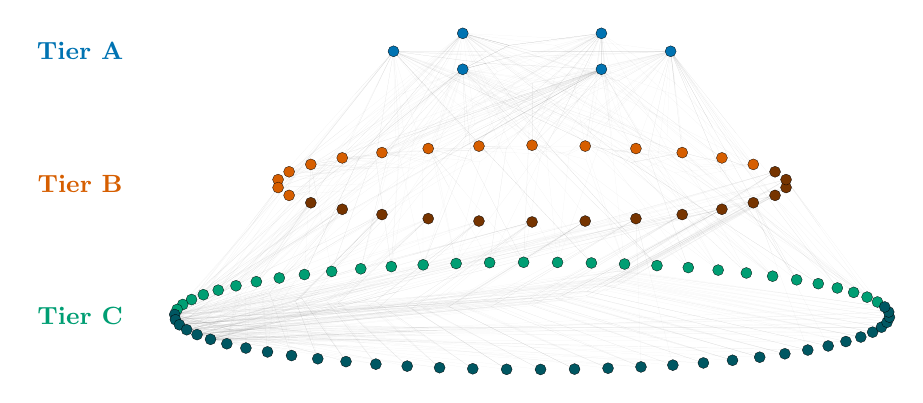
\begin{tikzpicture}[scale=1.4]
  \draw[gray, line width=0.08pt, opacity=0.10] (1.257,1.200) -- (0.419,1.309);
  \draw[gray, line width=0.08pt, opacity=0.10] (0.629,1.363) -- (0.419,1.309);
  \draw[gray, line width=0.08pt, opacity=0.10] (-0.629,1.363) -- (0.419,1.309);
  \draw[gray, line width=0.08pt, opacity=0.10] (1.257,1.200) -- (-0.000,1.200);
  \draw[gray, line width=0.08pt, opacity=0.10] (-0.629,1.363) -- (-0.000,1.200);
  \draw[gray, line width=0.08pt, opacity=0.10] (-0.629,1.037) -- (-0.000,1.200);
  \draw[gray, line width=0.08pt, opacity=0.10] (1.257,1.200) -- (-0.000,1.200);
  \draw[gray, line width=0.08pt, opacity=0.10] (-0.629,1.037) -- (-0.000,1.200);
  \draw[gray, line width=0.08pt, opacity=0.10] (-0.629,1.363) -- (-0.000,1.200);
  \draw[gray, line width=0.08pt, opacity=0.10] (1.257,1.200) -- (1.507,0.858);
  \draw[gray, line width=0.08pt, opacity=0.10] (2.007,0.174) -- (1.507,0.858);
  \draw[gray, line width=0.08pt, opacity=0.10] (1.257,1.200) -- (1.507,0.858);
  \draw[gray, line width=0.08pt, opacity=0.10] (1.257,1.200) -- (1.412,0.878);
  \draw[gray, line width=0.08pt, opacity=0.10] (1.722,0.233) -- (1.412,0.878);
  \draw[gray, line width=0.08pt, opacity=0.10] (1.257,1.200) -- (1.412,0.878);
  \draw[gray, line width=0.08pt, opacity=0.10] (1.257,1.200) -- (1.292,0.894);
  \draw[gray, line width=0.08pt, opacity=0.10] (1.362,0.281) -- (1.292,0.894);
  \draw[gray, line width=0.08pt, opacity=0.10] (1.257,1.200) -- (1.292,0.894);
  \draw[gray, line width=0.08pt, opacity=0.10] (1.257,1.200) -- (1.152,0.906);
  \draw[gray, line width=0.08pt, opacity=0.10] (0.942,0.318) -- (1.152,0.906);
  \draw[gray, line width=0.08pt, opacity=0.10] (1.257,1.200) -- (1.152,0.906);
  \draw[gray, line width=0.08pt, opacity=0.10] (1.257,1.200) -- (0.999,0.913);
  \draw[gray, line width=0.08pt, opacity=0.10] (0.482,0.340) -- (0.999,0.913);
  \draw[gray, line width=0.08pt, opacity=0.10] (1.257,1.200) -- (0.999,0.913);
  \draw[gray, line width=0.08pt, opacity=0.10] (1.257,1.200) -- (1.851,0.457);
  \draw[gray, line width=0.08pt, opacity=0.10] (3.039,-1.030) -- (1.851,0.457);
  \draw[gray, line width=0.08pt, opacity=0.10] (1.257,1.200) -- (1.851,0.457);
  \draw[gray, line width=0.08pt, opacity=0.10] (1.257,1.200) -- (1.761,0.484);
  \draw[gray, line width=0.08pt, opacity=0.10] (2.769,-0.947) -- (1.761,0.484);
  \draw[gray, line width=0.08pt, opacity=0.10] (1.257,1.200) -- (1.761,0.484);
  \draw[gray, line width=0.08pt, opacity=0.10] (1.257,1.200) -- (1.638,0.509);
  \draw[gray, line width=0.08pt, opacity=0.10] (2.400,-0.873) -- (1.638,0.509);
  \draw[gray, line width=0.08pt, opacity=0.10] (1.257,1.200) -- (1.638,0.509);
  \draw[gray, line width=0.08pt, opacity=0.10] (1.257,1.200) -- (1.673,0.203);
  \draw[gray, line width=0.08pt, opacity=0.10] (2.400,-0.873) -- (1.673,0.203);
  \draw[gray, line width=0.08pt, opacity=0.10] (1.362,0.281) -- (1.673,0.203);
  \draw[gray, line width=0.08pt, opacity=0.10] (1.257,1.200) -- (1.381,0.236);
  \draw[gray, line width=0.08pt, opacity=0.10] (1.944,-0.811) -- (1.381,0.236);
  \draw[gray, line width=0.08pt, opacity=0.10] (0.942,0.318) -- (1.381,0.236);
  \draw[gray, line width=0.08pt, opacity=0.10] (1.257,1.200) -- (1.052,0.259);
  \draw[gray, line width=0.08pt, opacity=0.10] (1.417,-0.762) -- (1.052,0.259);
  \draw[gray, line width=0.08pt, opacity=0.10] (0.482,0.340) -- (1.052,0.259);
  \draw[gray, line width=0.08pt, opacity=0.10] (0.629,1.363) -- (-0.210,1.254);
  \draw[gray, line width=0.08pt, opacity=0.10] (-0.629,1.363) -- (-0.210,1.254);
  \draw[gray, line width=0.08pt, opacity=0.10] (-0.629,1.037) -- (-0.210,1.254);
  \draw[gray, line width=0.08pt, opacity=0.10] (0.629,1.363) -- (-0.210,1.254);
  \draw[gray, line width=0.08pt, opacity=0.10] (-0.629,1.037) -- (-0.210,1.254);
  \draw[gray, line width=0.08pt, opacity=0.10] (-0.629,1.363) -- (-0.210,1.254);
  \draw[gray, line width=0.08pt, opacity=0.10] (0.629,1.363) -- (1.298,0.912);
  \draw[gray, line width=0.08pt, opacity=0.10] (2.007,0.174) -- (1.298,0.912);
  \draw[gray, line width=0.08pt, opacity=0.10] (1.257,1.200) -- (1.298,0.912);
  \draw[gray, line width=0.08pt, opacity=0.10] (0.629,1.363) -- (0.629,0.970);
  \draw[gray, line width=0.08pt, opacity=0.10] (0.000,0.348) -- (0.629,0.970);
  \draw[gray, line width=0.08pt, opacity=0.10] (1.257,1.200) -- (0.629,0.970);
  \draw[gray, line width=0.08pt, opacity=0.10] (0.629,1.363) -- (0.468,0.968);
  \draw[gray, line width=0.08pt, opacity=0.10] (-0.482,0.340) -- (0.468,0.968);
  \draw[gray, line width=0.08pt, opacity=0.10] (1.257,1.200) -- (0.468,0.968);
  \draw[gray, line width=0.08pt, opacity=0.10] (0.629,1.363) -- (0.315,0.960);
  \draw[gray, line width=0.08pt, opacity=0.10] (-0.942,0.318) -- (0.315,0.960);
  \draw[gray, line width=0.08pt, opacity=0.10] (1.257,1.200) -- (0.315,0.960);
  \draw[gray, line width=0.08pt, opacity=0.10] (0.629,1.363) -- (0.175,0.948);
  \draw[gray, line width=0.08pt, opacity=0.10] (-1.362,0.281) -- (0.175,0.948);
  \draw[gray, line width=0.08pt, opacity=0.10] (1.257,1.200) -- (0.175,0.948);
  \draw[gray, line width=0.08pt, opacity=0.10] (0.629,1.363) -- (-0.574,0.303);
  \draw[gray, line width=0.08pt, opacity=0.10] (-1.362,0.281) -- (-0.574,0.303);
  \draw[gray, line width=0.08pt, opacity=0.10] (-0.988,-0.737) -- (-0.574,0.303);
  \draw[gray, line width=0.08pt, opacity=0.10] (0.629,1.363) -- (1.923,0.154);
  \draw[gray, line width=0.08pt, opacity=0.10] (3.133,-1.074) -- (1.923,0.154);
  \draw[gray, line width=0.08pt, opacity=0.10] (2.007,0.174) -- (1.923,0.154);
  \draw[gray, line width=0.08pt, opacity=0.10] (0.629,1.363) -- (0.489,0.327);
  \draw[gray, line width=0.08pt, opacity=0.10] (0.839,-0.730) -- (0.489,0.327);
  \draw[gray, line width=0.08pt, opacity=0.10] (0.000,0.348) -- (0.489,0.327);
  \draw[gray, line width=0.08pt, opacity=0.10] (0.629,1.363) -- (0.126,0.330);
  \draw[gray, line width=0.08pt, opacity=0.10] (0.231,-0.715) -- (0.126,0.330);
  \draw[gray, line width=0.08pt, opacity=0.10] (-0.482,0.340) -- (0.126,0.330);
  \draw[gray, line width=0.08pt, opacity=0.10] (0.629,1.363) -- (-0.233,0.321);
  \draw[gray, line width=0.08pt, opacity=0.10] (-0.385,-0.717) -- (-0.233,0.321);
  \draw[gray, line width=0.08pt, opacity=0.10] (-0.942,0.318) -- (-0.233,0.321);
  \draw[gray, line width=0.08pt, opacity=0.10] (0.629,1.363) -- (-0.574,0.303);
  \draw[gray, line width=0.08pt, opacity=0.10] (-0.988,-0.737) -- (-0.574,0.303);
  \draw[gray, line width=0.08pt, opacity=0.10] (-1.362,0.281) -- (-0.574,0.303);
  \draw[gray, line width=0.08pt, opacity=0.10] (-0.629,1.363) -- (-0.210,1.254);
  \draw[gray, line width=0.08pt, opacity=0.10] (0.629,1.363) -- (-0.210,1.254);
  \draw[gray, line width=0.08pt, opacity=0.10] (-0.629,1.037) -- (-0.210,1.254);
  \draw[gray, line width=0.08pt, opacity=0.10] (-0.629,1.363) -- (-0.210,1.254);
  \draw[gray, line width=0.08pt, opacity=0.10] (-0.629,1.037) -- (-0.210,1.254);
  \draw[gray, line width=0.08pt, opacity=0.10] (0.629,1.363) -- (-0.210,1.254);
  \draw[gray, line width=0.08pt, opacity=0.10] (-0.629,1.363) -- (0.784,0.932);
  \draw[gray, line width=0.08pt, opacity=0.10] (1.722,0.233) -- (0.784,0.932);
  \draw[gray, line width=0.08pt, opacity=0.10] (1.257,1.200) -- (0.784,0.932);
  \draw[gray, line width=0.08pt, opacity=0.10] (-0.629,1.363) -- (0.210,0.970);
  \draw[gray, line width=0.08pt, opacity=0.10] (0.000,0.348) -- (0.210,0.970);
  \draw[gray, line width=0.08pt, opacity=0.10] (1.257,1.200) -- (0.210,0.970);
  \draw[gray, line width=0.08pt, opacity=0.10] (-0.629,1.363) -- (0.168,0.322);
  \draw[gray, line width=0.08pt, opacity=0.10] (0.000,0.348) -- (0.168,0.322);
  \draw[gray, line width=0.08pt, opacity=0.10] (1.133,-0.744) -- (0.168,0.322);
  \draw[gray, line width=0.08pt, opacity=0.10] (-0.629,1.363) -- (-1.302,0.274);
  \draw[gray, line width=0.08pt, opacity=0.10] (-1.722,0.233) -- (-1.302,0.274);
  \draw[gray, line width=0.08pt, opacity=0.10] (-1.554,-0.773) -- (-1.302,0.274);
  \draw[gray, line width=0.08pt, opacity=0.10] (-0.629,1.363) -- (-1.567,0.237);
  \draw[gray, line width=0.08pt, opacity=0.10] (-2.007,0.174) -- (-1.567,0.237);
  \draw[gray, line width=0.08pt, opacity=0.10] (-2.065,-0.825) -- (-1.567,0.237);
  \draw[gray, line width=0.08pt, opacity=0.10] (-0.629,1.363) -- (-1.778,0.193);
  \draw[gray, line width=0.08pt, opacity=0.10] (-2.204,0.107) -- (-1.778,0.193);
  \draw[gray, line width=0.08pt, opacity=0.10] (-2.501,-0.890) -- (-1.778,0.193);
  \draw[gray, line width=0.08pt, opacity=0.10] (-0.629,1.363) -- (1.337,0.203);
  \draw[gray, line width=0.08pt, opacity=0.10] (2.917,-0.987) -- (1.337,0.203);
  \draw[gray, line width=0.08pt, opacity=0.10] (1.722,0.233) -- (1.337,0.203);
  \draw[gray, line width=0.08pt, opacity=0.10] (-0.629,1.363) -- (0.168,0.322);
  \draw[gray, line width=0.08pt, opacity=0.10] (1.133,-0.744) -- (0.168,0.322);
  \draw[gray, line width=0.08pt, opacity=0.10] (0.000,0.348) -- (0.168,0.322);
  \draw[gray, line width=0.08pt, opacity=0.10] (-0.629,1.363) -- (-1.302,0.274);
  \draw[gray, line width=0.08pt, opacity=0.10] (-1.554,-0.773) -- (-1.302,0.274);
  \draw[gray, line width=0.08pt, opacity=0.10] (-1.722,0.233) -- (-1.302,0.274);
  \draw[gray, line width=0.08pt, opacity=0.10] (-0.629,1.363) -- (-1.567,0.237);
  \draw[gray, line width=0.08pt, opacity=0.10] (-2.065,-0.825) -- (-1.567,0.237);
  \draw[gray, line width=0.08pt, opacity=0.10] (-2.007,0.174) -- (-1.567,0.237);
  \draw[gray, line width=0.08pt, opacity=0.10] (-0.629,1.363) -- (-1.778,0.193);
  \draw[gray, line width=0.08pt, opacity=0.10] (-2.501,-0.890) -- (-1.778,0.193);
  \draw[gray, line width=0.08pt, opacity=0.10] (-2.204,0.107) -- (-1.778,0.193);
  \draw[gray, line width=0.08pt, opacity=0.10] (-1.257,1.200) -- (-0.419,1.200);
  \draw[gray, line width=0.08pt, opacity=0.10] (0.629,1.363) -- (-0.419,1.200);
  \draw[gray, line width=0.08pt, opacity=0.10] (-0.629,1.037) -- (-0.419,1.200);
  \draw[gray, line width=0.08pt, opacity=0.10] (-1.257,1.200) -- (-0.210,1.146);
  \draw[gray, line width=0.08pt, opacity=0.10] (-0.629,1.037) -- (-0.210,1.146);
  \draw[gray, line width=0.08pt, opacity=0.10] (1.257,1.200) -- (-0.210,1.146);
  \draw[gray, line width=0.08pt, opacity=0.10] (-1.257,1.200) -- (-0.419,1.091);
  \draw[gray, line width=0.08pt, opacity=0.10] (0.629,1.037) -- (-0.419,1.091);
  \draw[gray, line width=0.08pt, opacity=0.10] (-0.629,1.037) -- (-0.419,1.091);
  \draw[gray, line width=0.08pt, opacity=0.10] (-1.257,1.200) -- (0.900,0.191);
  \draw[gray, line width=0.08pt, opacity=0.10] (1.362,0.281) -- (0.900,0.191);
  \draw[gray, line width=0.08pt, opacity=0.10] (2.596,-0.908) -- (0.900,0.191);
  \draw[gray, line width=0.08pt, opacity=0.10] (-1.257,1.200) -- (-0.400,0.273);
  \draw[gray, line width=0.08pt, opacity=0.10] (-0.482,0.340) -- (-0.400,0.273);
  \draw[gray, line width=0.08pt, opacity=0.10] (0.538,-0.720) -- (-0.400,0.273);
  \draw[gray, line width=0.08pt, opacity=0.10] (-1.257,1.200) -- (-1.419,0.227);
  \draw[gray, line width=0.08pt, opacity=0.10] (-1.722,0.233) -- (-1.419,0.227);
  \draw[gray, line width=0.08pt, opacity=0.10] (-1.277,-0.753) -- (-1.419,0.227);
  \draw[gray, line width=0.08pt, opacity=0.10] (-1.257,1.200) -- (-2.136,0.090);
  \draw[gray, line width=0.08pt, opacity=0.10] (-2.304,0.036) -- (-2.136,0.090);
  \draw[gray, line width=0.08pt, opacity=0.10] (-2.847,-0.967) -- (-2.136,0.090);
  \draw[gray, line width=0.08pt, opacity=0.10] (-1.257,1.200) -- (-2.217,0.037);
  \draw[gray, line width=0.08pt, opacity=0.10] (-2.304,-0.036) -- (-2.217,0.037);
  \draw[gray, line width=0.08pt, opacity=0.10] (-3.089,-1.052) -- (-2.217,0.037);
  \draw[gray, line width=0.08pt, opacity=0.10] (-1.257,1.200) -- (0.900,0.191);
  \draw[gray, line width=0.08pt, opacity=0.10] (2.596,-0.908) -- (0.900,0.191);
  \draw[gray, line width=0.08pt, opacity=0.10] (1.362,0.281) -- (0.900,0.191);
  \draw[gray, line width=0.08pt, opacity=0.10] (-1.257,1.200) -- (-0.400,0.273);
  \draw[gray, line width=0.08pt, opacity=0.10] (0.538,-0.720) -- (-0.400,0.273);
  \draw[gray, line width=0.08pt, opacity=0.10] (-0.482,0.340) -- (-0.400,0.273);
  \draw[gray, line width=0.08pt, opacity=0.10] (-1.257,1.200) -- (-1.419,0.227);
  \draw[gray, line width=0.08pt, opacity=0.10] (-1.277,-0.753) -- (-1.419,0.227);
  \draw[gray, line width=0.08pt, opacity=0.10] (-1.722,0.233) -- (-1.419,0.227);
  \draw[gray, line width=0.08pt, opacity=0.10] (-1.257,1.200) -- (-1.158,0.423);
  \draw[gray, line width=0.08pt, opacity=0.10] (-2.847,-0.967) -- (-1.158,0.423);
  \draw[gray, line width=0.08pt, opacity=0.10] (0.629,1.037) -- (-1.158,0.423);
  \draw[gray, line width=0.08pt, opacity=0.10] (-1.257,1.200) -- (-1.239,0.395);
  \draw[gray, line width=0.08pt, opacity=0.10] (-3.089,-1.052) -- (-1.239,0.395);
  \draw[gray, line width=0.08pt, opacity=0.10] (0.629,1.037) -- (-1.239,0.395);
  \draw[gray, line width=0.08pt, opacity=0.10] (-0.629,1.037) -- (-0.210,1.254);
  \draw[gray, line width=0.08pt, opacity=0.10] (0.629,1.363) -- (-0.210,1.254);
  \draw[gray, line width=0.08pt, opacity=0.10] (-0.629,1.363) -- (-0.210,1.254);
  \draw[gray, line width=0.08pt, opacity=0.10] (-0.629,1.037) -- (-0.210,1.146);
  \draw[gray, line width=0.08pt, opacity=0.10] (-1.257,1.200) -- (-0.210,1.146);
  \draw[gray, line width=0.08pt, opacity=0.10] (1.257,1.200) -- (-0.210,1.146);
  \draw[gray, line width=0.08pt, opacity=0.10] (-0.629,1.037) -- (-0.419,1.091);
  \draw[gray, line width=0.08pt, opacity=0.10] (0.629,1.037) -- (-0.419,1.091);
  \draw[gray, line width=0.08pt, opacity=0.10] (-1.257,1.200) -- (-0.419,1.091);
  \draw[gray, line width=0.08pt, opacity=0.10] (-0.629,1.037) -- (0.832,0.171);
  \draw[gray, line width=0.08pt, opacity=0.10] (0.942,0.318) -- (0.832,0.171);
  \draw[gray, line width=0.08pt, opacity=0.10] (2.182,-0.840) -- (0.832,0.171);
  \draw[gray, line width=0.08pt, opacity=0.10] (-0.629,1.037) -- (-0.549,0.214);
  \draw[gray, line width=0.08pt, opacity=0.10] (-0.942,0.318) -- (-0.549,0.214);
  \draw[gray, line width=0.08pt, opacity=0.10] (-0.077,-0.714) -- (-0.549,0.214);
  \draw[gray, line width=0.08pt, opacity=0.10] (-0.629,1.037) -- (-1.484,0.138);
  \draw[gray, line width=0.08pt, opacity=0.10] (-2.007,0.174) -- (-1.484,0.138);
  \draw[gray, line width=0.08pt, opacity=0.10] (-1.818,-0.797) -- (-1.484,0.138);
  \draw[gray, line width=0.08pt, opacity=0.10] (-0.629,1.037) -- (-1.873,0.049);
  \draw[gray, line width=0.08pt, opacity=0.10] (-2.304,0.036) -- (-1.873,0.049);
  \draw[gray, line width=0.08pt, opacity=0.10] (-2.686,-0.927) -- (-1.873,0.049);
  \draw[gray, line width=0.08pt, opacity=0.10] (-0.629,1.037) -- (-2.018,-0.071);
  \draw[gray, line width=0.08pt, opacity=0.10] (-2.204,-0.107) -- (-2.018,-0.071);
  \draw[gray, line width=0.08pt, opacity=0.10] (-3.220,-1.142) -- (-2.018,-0.071);
  \draw[gray, line width=0.08pt, opacity=0.10] (-0.629,1.037) -- (0.727,0.411);
  \draw[gray, line width=0.08pt, opacity=0.10] (2.182,-0.840) -- (0.727,0.411);
  \draw[gray, line width=0.08pt, opacity=0.10] (0.629,1.037) -- (0.727,0.411);
  \draw[gray, line width=0.08pt, opacity=0.10] (-0.629,1.037) -- (-0.026,0.453);
  \draw[gray, line width=0.08pt, opacity=0.10] (-0.077,-0.714) -- (-0.026,0.453);
  \draw[gray, line width=0.08pt, opacity=0.10] (0.629,1.037) -- (-0.026,0.453);
  \draw[gray, line width=0.08pt, opacity=0.10] (-0.629,1.037) -- (-0.606,0.425);
  \draw[gray, line width=0.08pt, opacity=0.10] (-1.818,-0.797) -- (-0.606,0.425);
  \draw[gray, line width=0.08pt, opacity=0.10] (0.629,1.037) -- (-0.606,0.425);
  \draw[gray, line width=0.08pt, opacity=0.10] (-0.629,1.037) -- (-0.895,0.382);
  \draw[gray, line width=0.08pt, opacity=0.10] (-2.686,-0.927) -- (-0.895,0.382);
  \draw[gray, line width=0.08pt, opacity=0.10] (0.629,1.037) -- (-0.895,0.382);
  \draw[gray, line width=0.08pt, opacity=0.10] (-0.629,1.037) -- (-1.073,0.310);
  \draw[gray, line width=0.08pt, opacity=0.10] (-3.220,-1.142) -- (-1.073,0.310);
  \draw[gray, line width=0.08pt, opacity=0.10] (0.629,1.037) -- (-1.073,0.310);
  \draw[gray, line width=0.08pt, opacity=0.10] (0.629,1.037) -- (0.210,1.254);
  \draw[gray, line width=0.08pt, opacity=0.10] (0.629,1.363) -- (0.210,1.254);
  \draw[gray, line width=0.08pt, opacity=0.10] (-0.629,1.363) -- (0.210,1.254);
  \draw[gray, line width=0.08pt, opacity=0.10] (0.629,1.037) -- (0.210,1.146);
  \draw[gray, line width=0.08pt, opacity=0.10] (-1.257,1.200) -- (0.210,1.146);
  \draw[gray, line width=0.08pt, opacity=0.10] (1.257,1.200) -- (0.210,1.146);
  \draw[gray, line width=0.08pt, opacity=0.10] (0.629,1.037) -- (-0.419,1.091);
  \draw[gray, line width=0.08pt, opacity=0.10] (-0.629,1.037) -- (-0.419,1.091);
  \draw[gray, line width=0.08pt, opacity=0.10] (-1.257,1.200) -- (-0.419,1.091);
  \draw[gray, line width=0.08pt, opacity=0.10] (0.629,1.037) -- (0.933,0.197);
  \draw[gray, line width=0.08pt, opacity=0.10] (0.482,0.340) -- (0.933,0.197);
  \draw[gray, line width=0.08pt, opacity=0.10] (1.688,-0.785) -- (0.933,0.197);
  \draw[gray, line width=0.08pt, opacity=0.10] (0.629,1.037) -- (-0.474,0.198);
  \draw[gray, line width=0.08pt, opacity=0.10] (-1.362,0.281) -- (-0.474,0.198);
  \draw[gray, line width=0.08pt, opacity=0.10] (-0.689,-0.725) -- (-0.474,0.198);
  \draw[gray, line width=0.08pt, opacity=0.10] (0.629,1.037) -- (-0.315,0.727);
  \draw[gray, line width=0.08pt, opacity=0.10] (-2.204,0.107) -- (-0.315,0.727);
  \draw[gray, line width=0.08pt, opacity=0.10] (0.629,1.037) -- (-0.315,0.727);
  \draw[gray, line width=0.08pt, opacity=0.10] (0.629,1.037) -- (-0.349,0.679);
  \draw[gray, line width=0.08pt, opacity=0.10] (-2.304,-0.036) -- (-0.349,0.679);
  \draw[gray, line width=0.08pt, opacity=0.10] (0.629,1.037) -- (-0.349,0.679);
  \draw[gray, line width=0.08pt, opacity=0.10] (0.629,1.037) -- (-0.315,0.655);
  \draw[gray, line width=0.08pt, opacity=0.10] (-2.204,-0.107) -- (-0.315,0.655);
  \draw[gray, line width=0.08pt, opacity=0.10] (0.629,1.037) -- (-0.315,0.655);
  \draw[gray, line width=0.08pt, opacity=0.10] (0.629,1.037) -- (0.982,0.430);
  \draw[gray, line width=0.08pt, opacity=0.10] (1.688,-0.785) -- (0.982,0.430);
  \draw[gray, line width=0.08pt, opacity=0.10] (0.629,1.037) -- (0.982,0.430);
  \draw[gray, line width=0.08pt, opacity=0.10] (0.629,1.037) -- (0.189,0.450);
  \draw[gray, line width=0.08pt, opacity=0.10] (-0.689,-0.725) -- (0.189,0.450);
  \draw[gray, line width=0.08pt, opacity=0.10] (0.629,1.037) -- (0.189,0.450);
  \draw[gray, line width=0.08pt, opacity=0.10] (0.629,1.037) -- (-0.345,0.406);
  \draw[gray, line width=0.08pt, opacity=0.10] (-2.293,-0.856) -- (-0.345,0.406);
  \draw[gray, line width=0.08pt, opacity=0.10] (0.629,1.037) -- (-0.345,0.406);
  \draw[gray, line width=0.08pt, opacity=0.10] (0.629,1.037) -- (-0.575,0.355);
  \draw[gray, line width=0.08pt, opacity=0.10] (-2.982,-1.008) -- (-0.575,0.355);
  \draw[gray, line width=0.08pt, opacity=0.10] (0.629,1.037) -- (-0.575,0.355);
  \draw[gray, line width=0.08pt, opacity=0.10] (0.629,1.037) -- (-0.637,0.326);
  \draw[gray, line width=0.08pt, opacity=0.10] (-3.169,-1.097) -- (-0.637,0.326);
  \draw[gray, line width=0.08pt, opacity=0.10] (0.629,1.037) -- (-0.637,0.326);
  \draw[gray, line width=0.08pt, opacity=0.10] (2.007,0.174) -- (1.298,0.803);
  \draw[gray, line width=0.08pt, opacity=0.10] (1.257,1.200) -- (1.298,0.803);
  \draw[gray, line width=0.08pt, opacity=0.10] (0.629,1.037) -- (1.298,0.803);
  \draw[gray, line width=0.08pt, opacity=0.10] (2.007,0.174) -- (0.669,0.858);
  \draw[gray, line width=0.08pt, opacity=0.10] (0.629,1.363) -- (0.669,0.858);
  \draw[gray, line width=0.08pt, opacity=0.10] (-0.629,1.037) -- (0.669,0.858);
  \draw[gray, line width=0.08pt, opacity=0.10] (2.007,0.174) -- (1.504,0.154);
  \draw[gray, line width=0.08pt, opacity=0.10] (3.133,-1.074) -- (1.504,0.154);
  \draw[gray, line width=0.08pt, opacity=0.10] (-0.629,1.363) -- (1.504,0.154);
  \draw[gray, line width=0.08pt, opacity=0.10] (2.007,0.174) -- (1.472,0.169);
  \draw[gray, line width=0.08pt, opacity=0.10] (3.039,-1.030) -- (1.472,0.169);
  \draw[gray, line width=0.08pt, opacity=0.10] (-0.629,1.363) -- (1.472,0.169);
  \draw[gray, line width=0.08pt, opacity=0.10] (1.722,0.233) -- (0.784,0.932);
  \draw[gray, line width=0.08pt, opacity=0.10] (1.257,1.200) -- (0.784,0.932);
  \draw[gray, line width=0.08pt, opacity=0.10] (-0.629,1.363) -- (0.784,0.932);
  \draw[gray, line width=0.08pt, opacity=0.10] (1.722,0.233) -- (0.574,0.986);
  \draw[gray, line width=0.08pt, opacity=0.10] (-0.629,1.363) -- (0.574,0.986);
  \draw[gray, line width=0.08pt, opacity=0.10] (0.629,1.363) -- (0.574,0.986);
  \draw[gray, line width=0.08pt, opacity=0.10] (1.722,0.233) -- (1.966,0.148);
  \draw[gray, line width=0.08pt, opacity=0.10] (2.917,-0.987) -- (1.966,0.148);
  \draw[gray, line width=0.08pt, opacity=0.10] (1.257,1.200) -- (1.966,0.148);
  \draw[gray, line width=0.08pt, opacity=0.10] (1.722,0.233) -- (1.916,0.162);
  \draw[gray, line width=0.08pt, opacity=0.10] (2.769,-0.947) -- (1.916,0.162);
  \draw[gray, line width=0.08pt, opacity=0.10] (1.257,1.200) -- (1.916,0.162);
  \draw[gray, line width=0.08pt, opacity=0.10] (1.362,0.281) -- (1.292,0.894);
  \draw[gray, line width=0.08pt, opacity=0.10] (1.257,1.200) -- (1.292,0.894);
  \draw[gray, line width=0.08pt, opacity=0.10] (1.257,1.200) -- (1.292,0.894);
  \draw[gray, line width=0.08pt, opacity=0.10] (1.362,0.281) -- (1.673,0.203);
  \draw[gray, line width=0.08pt, opacity=0.10] (1.257,1.200) -- (1.673,0.203);
  \draw[gray, line width=0.08pt, opacity=0.10] (2.400,-0.873) -- (1.673,0.203);
  \draw[gray, line width=0.08pt, opacity=0.10] (1.362,0.281) -- (0.489,0.587);
  \draw[gray, line width=0.08pt, opacity=0.10] (-1.257,1.200) -- (0.489,0.587);
  \draw[gray, line width=0.08pt, opacity=0.10] (1.362,0.281) -- (0.489,0.587);
  \draw[gray, line width=0.08pt, opacity=0.10] (1.362,0.281) -- (1.529,0.136);
  \draw[gray, line width=0.08pt, opacity=0.10] (2.596,-0.908) -- (1.529,0.136);
  \draw[gray, line width=0.08pt, opacity=0.10] (0.629,1.037) -- (1.529,0.136);
  \draw[gray, line width=0.08pt, opacity=0.10] (1.362,0.281) -- (1.044,0.148);
  \draw[gray, line width=0.08pt, opacity=0.10] (2.400,-0.873) -- (1.044,0.148);
  \draw[gray, line width=0.08pt, opacity=0.10] (-0.629,1.037) -- (1.044,0.148);
  \draw[gray, line width=0.08pt, opacity=0.10] (0.942,0.318) -- (0.524,0.851);
  \draw[gray, line width=0.08pt, opacity=0.10] (1.257,1.200) -- (0.524,0.851);
  \draw[gray, line width=0.08pt, opacity=0.10] (-0.629,1.037) -- (0.524,0.851);
  \draw[gray, line width=0.08pt, opacity=0.10] (0.942,0.318) -- (-0.315,0.851);
  \draw[gray, line width=0.08pt, opacity=0.10] (-0.629,1.037) -- (-0.315,0.851);
  \draw[gray, line width=0.08pt, opacity=0.10] (-1.257,1.200) -- (-0.315,0.851);
  \draw[gray, line width=0.08pt, opacity=0.10] (0.942,0.318) -- (0.832,0.280);
  \draw[gray, line width=0.08pt, opacity=0.10] (2.182,-0.840) -- (0.832,0.280);
  \draw[gray, line width=0.08pt, opacity=0.10] (-0.629,1.363) -- (0.832,0.280);
  \draw[gray, line width=0.08pt, opacity=0.10] (0.942,0.318) -- (0.752,0.290);
  \draw[gray, line width=0.08pt, opacity=0.10] (1.944,-0.811) -- (0.752,0.290);
  \draw[gray, line width=0.08pt, opacity=0.10] (-0.629,1.363) -- (0.752,0.290);
  \draw[gray, line width=0.08pt, opacity=0.10] (0.482,0.340) -- (0.370,0.968);
  \draw[gray, line width=0.08pt, opacity=0.10] (1.257,1.200) -- (0.370,0.968);
  \draw[gray, line width=0.08pt, opacity=0.10] (-0.629,1.363) -- (0.370,0.968);
  \draw[gray, line width=0.08pt, opacity=0.10] (0.482,0.340) -- (0.580,0.913);
  \draw[gray, line width=0.08pt, opacity=0.10] (0.629,1.037) -- (0.580,0.913);
  \draw[gray, line width=0.08pt, opacity=0.10] (0.629,1.363) -- (0.580,0.913);
  \draw[gray, line width=0.08pt, opacity=0.10] (0.482,0.340) -- (1.142,0.252);
  \draw[gray, line width=0.08pt, opacity=0.10] (1.688,-0.785) -- (1.142,0.252);
  \draw[gray, line width=0.08pt, opacity=0.10] (1.257,1.200) -- (1.142,0.252);
  \draw[gray, line width=0.08pt, opacity=0.10] (0.482,0.340) -- (1.052,0.259);
  \draw[gray, line width=0.08pt, opacity=0.10] (1.417,-0.762) -- (1.052,0.259);
  \draw[gray, line width=0.08pt, opacity=0.10] (1.257,1.200) -- (1.052,0.259);
  \draw[gray, line width=0.08pt, opacity=0.10] (0.000,0.348) -- (0.629,0.970);
  \draw[gray, line width=0.08pt, opacity=0.10] (0.629,1.363) -- (0.629,0.970);
  \draw[gray, line width=0.08pt, opacity=0.10] (1.257,1.200) -- (0.629,0.970);
  \draw[gray, line width=0.08pt, opacity=0.10] (0.000,0.348) -- (0.210,0.686);
  \draw[gray, line width=0.08pt, opacity=0.10] (0.629,1.363) -- (0.210,0.686);
  \draw[gray, line width=0.08pt, opacity=0.10] (0.000,0.348) -- (0.210,0.686);
  \draw[gray, line width=0.08pt, opacity=0.10] (0.000,0.348) -- (0.000,0.916);
  \draw[gray, line width=0.08pt, opacity=0.10] (-0.629,1.363) -- (0.000,0.916);
  \draw[gray, line width=0.08pt, opacity=0.10] (0.629,1.037) -- (0.000,0.916);
  \draw[gray, line width=0.08pt, opacity=0.10] (0.000,0.348) -- (0.168,0.213);
  \draw[gray, line width=0.08pt, opacity=0.10] (1.133,-0.744) -- (0.168,0.213);
  \draw[gray, line width=0.08pt, opacity=0.10] (-0.629,1.037) -- (0.168,0.213);
  \draw[gray, line width=0.08pt, opacity=0.10] (0.000,0.348) -- (0.070,0.218);
  \draw[gray, line width=0.08pt, opacity=0.10] (0.839,-0.730) -- (0.070,0.218);
  \draw[gray, line width=0.08pt, opacity=0.10] (-0.629,1.037) -- (0.070,0.218);
  \draw[gray, line width=0.08pt, opacity=0.10] (-0.482,0.340) -- (-0.161,0.913);
  \draw[gray, line width=0.08pt, opacity=0.10] (0.629,1.363) -- (-0.161,0.913);
  \draw[gray, line width=0.08pt, opacity=0.10] (-0.629,1.037) -- (-0.161,0.913);
  \draw[gray, line width=0.08pt, opacity=0.10] (-0.482,0.340) -- (-0.999,0.913);
  \draw[gray, line width=0.08pt, opacity=0.10] (-1.257,1.200) -- (-0.999,0.913);
  \draw[gray, line width=0.08pt, opacity=0.10] (-1.257,1.200) -- (-0.999,0.913);
  \draw[gray, line width=0.08pt, opacity=0.10] (-0.482,0.340) -- (-0.191,0.328);
  \draw[gray, line width=0.08pt, opacity=0.10] (0.538,-0.720) -- (-0.191,0.328);
  \draw[gray, line width=0.08pt, opacity=0.10] (-0.629,1.363) -- (-0.191,0.328);
  \draw[gray, line width=0.08pt, opacity=0.10] (-0.482,0.340) -- (-0.293,0.330);
  \draw[gray, line width=0.08pt, opacity=0.10] (0.231,-0.715) -- (-0.293,0.330);
  \draw[gray, line width=0.08pt, opacity=0.10] (-0.629,1.363) -- (-0.293,0.330);
  \draw[gray, line width=0.08pt, opacity=0.10] (-0.942,0.318) -- (-0.314,1.015);
  \draw[gray, line width=0.08pt, opacity=0.10] (0.629,1.363) -- (-0.314,1.015);
  \draw[gray, line width=0.08pt, opacity=0.10] (-0.629,1.363) -- (-0.314,1.015);
  \draw[gray, line width=0.08pt, opacity=0.10] (-0.942,0.318) -- (-0.314,0.906);
  \draw[gray, line width=0.08pt, opacity=0.10] (-0.629,1.037) -- (-0.314,0.906);
  \draw[gray, line width=0.08pt, opacity=0.10] (0.629,1.363) -- (-0.314,0.906);
  \draw[gray, line width=0.08pt, opacity=0.10] (-0.942,0.318) -- (-0.549,0.214);
  \draw[gray, line width=0.08pt, opacity=0.10] (-0.629,1.037) -- (-0.549,0.214);
  \draw[gray, line width=0.08pt, opacity=0.10] (-0.077,-0.714) -- (-0.549,0.214);
  \draw[gray, line width=0.08pt, opacity=0.10] (-0.942,0.318) -- (-0.654,-0.026);
  \draw[gray, line width=0.08pt, opacity=0.10] (-0.077,-0.714) -- (-0.654,-0.026);
  \draw[gray, line width=0.08pt, opacity=0.10] (-0.942,0.318) -- (-0.654,-0.026);
  \draw[gray, line width=0.08pt, opacity=0.10] (-0.942,0.318) -- (-0.757,-0.027);
  \draw[gray, line width=0.08pt, opacity=0.10] (-0.385,-0.717) -- (-0.757,-0.027);
  \draw[gray, line width=0.08pt, opacity=0.10] (-0.942,0.318) -- (-0.757,-0.027);
  \draw[gray, line width=0.08pt, opacity=0.10] (-1.362,0.281) -- (-0.698,0.642);
  \draw[gray, line width=0.08pt, opacity=0.10] (0.629,1.363) -- (-0.698,0.642);
  \draw[gray, line width=0.08pt, opacity=0.10] (-1.362,0.281) -- (-0.698,0.642);
  \draw[gray, line width=0.08pt, opacity=0.10] (-1.362,0.281) -- (-0.035,0.785);
  \draw[gray, line width=0.08pt, opacity=0.10] (0.629,1.037) -- (-0.035,0.785);
  \draw[gray, line width=0.08pt, opacity=0.10] (0.629,1.037) -- (-0.035,0.785);
  \draw[gray, line width=0.08pt, opacity=0.10] (-1.362,0.281) -- (-0.893,0.198);
  \draw[gray, line width=0.08pt, opacity=0.10] (-0.689,-0.725) -- (-0.893,0.198);
  \draw[gray, line width=0.08pt, opacity=0.10] (-0.629,1.037) -- (-0.893,0.198);
  \draw[gray, line width=0.08pt, opacity=0.10] (-1.362,0.281) -- (-0.993,0.194);
  \draw[gray, line width=0.08pt, opacity=0.10] (-0.988,-0.737) -- (-0.993,0.194);
  \draw[gray, line width=0.08pt, opacity=0.10] (-0.629,1.037) -- (-0.993,0.194);
  \draw[gray, line width=0.08pt, opacity=0.10] (-1.722,0.233) -- (-0.993,0.878);
  \draw[gray, line width=0.08pt, opacity=0.10] (-0.629,1.363) -- (-0.993,0.878);
  \draw[gray, line width=0.08pt, opacity=0.10] (-0.629,1.037) -- (-0.993,0.878);
  \draw[gray, line width=0.08pt, opacity=0.10] (-1.722,0.233) -- (-1.412,0.878);
  \draw[gray, line width=0.08pt, opacity=0.10] (-1.257,1.200) -- (-1.412,0.878);
  \draw[gray, line width=0.08pt, opacity=0.10] (-1.257,1.200) -- (-1.412,0.878);
  \draw[gray, line width=0.08pt, opacity=0.10] (-1.722,0.233) -- (-1.209,0.281);
  \draw[gray, line width=0.08pt, opacity=0.10] (-1.277,-0.753) -- (-1.209,0.281);
  \draw[gray, line width=0.08pt, opacity=0.10] (-0.629,1.363) -- (-1.209,0.281);
  \draw[gray, line width=0.08pt, opacity=0.10] (-1.722,0.233) -- (-0.883,0.274);
  \draw[gray, line width=0.08pt, opacity=0.10] (-1.554,-0.773) -- (-0.883,0.274);
  \draw[gray, line width=0.08pt, opacity=0.10] (0.629,1.363) -- (-0.883,0.274);
  \draw[gray, line width=0.08pt, opacity=0.10] (-2.007,0.174) -- (-0.669,0.967);
  \draw[gray, line width=0.08pt, opacity=0.10] (-0.629,1.363) -- (-0.669,0.967);
  \draw[gray, line width=0.08pt, opacity=0.10] (0.629,1.363) -- (-0.669,0.967);
  \draw[gray, line width=0.08pt, opacity=0.10] (-2.007,0.174) -- (-0.459,0.803);
  \draw[gray, line width=0.08pt, opacity=0.10] (-0.629,1.037) -- (-0.459,0.803);
  \draw[gray, line width=0.08pt, opacity=0.10] (1.257,1.200) -- (-0.459,0.803);
  \draw[gray, line width=0.08pt, opacity=0.10] (-2.007,0.174) -- (-1.484,0.138);
  \draw[gray, line width=0.08pt, opacity=0.10] (-0.629,1.037) -- (-1.484,0.138);
  \draw[gray, line width=0.08pt, opacity=0.10] (-1.818,-0.797) -- (-1.484,0.138);
  \draw[gray, line width=0.08pt, opacity=0.10] (-2.007,0.174) -- (-1.944,-0.150);
  \draw[gray, line width=0.08pt, opacity=0.10] (-1.818,-0.797) -- (-1.944,-0.150);
  \draw[gray, line width=0.08pt, opacity=0.10] (-2.007,0.174) -- (-1.944,-0.150);
  \draw[gray, line width=0.08pt, opacity=0.10] (-2.007,0.174) -- (-2.026,-0.159);
  \draw[gray, line width=0.08pt, opacity=0.10] (-2.065,-0.825) -- (-2.026,-0.159);
  \draw[gray, line width=0.08pt, opacity=0.10] (-2.007,0.174) -- (-2.026,-0.159);
  \draw[gray, line width=0.08pt, opacity=0.10] (-2.204,0.107) -- (-1.679,0.526);
  \draw[gray, line width=0.08pt, opacity=0.10] (-0.629,1.363) -- (-1.679,0.526);
  \draw[gray, line width=0.08pt, opacity=0.10] (-2.204,0.107) -- (-1.679,0.526);
  \draw[gray, line width=0.08pt, opacity=0.10] (-2.204,0.107) -- (-0.315,0.727);
  \draw[gray, line width=0.08pt, opacity=0.10] (0.629,1.037) -- (-0.315,0.727);
  \draw[gray, line width=0.08pt, opacity=0.10] (0.629,1.037) -- (-0.315,0.727);
  \draw[gray, line width=0.08pt, opacity=0.10] (-2.204,0.107) -- (-1.709,0.096);
  \draw[gray, line width=0.08pt, opacity=0.10] (-2.293,-0.856) -- (-1.709,0.096);
  \draw[gray, line width=0.08pt, opacity=0.10] (-0.629,1.037) -- (-1.709,0.096);
  \draw[gray, line width=0.08pt, opacity=0.10] (-2.204,0.107) -- (-1.778,0.085);
  \draw[gray, line width=0.08pt, opacity=0.10] (-2.501,-0.890) -- (-1.778,0.085);
  \draw[gray, line width=0.08pt, opacity=0.10] (-0.629,1.037) -- (-1.778,0.085);
  \draw[gray, line width=0.08pt, opacity=0.10] (-2.304,0.036) -- (-1.606,0.812);
  \draw[gray, line width=0.08pt, opacity=0.10] (-1.257,1.200) -- (-1.606,0.812);
  \draw[gray, line width=0.08pt, opacity=0.10] (-1.257,1.200) -- (-1.606,0.812);
  \draw[gray, line width=0.08pt, opacity=0.10] (-2.304,0.036) -- (-1.187,0.812);
  \draw[gray, line width=0.08pt, opacity=0.10] (-0.629,1.037) -- (-1.187,0.812);
  \draw[gray, line width=0.08pt, opacity=0.10] (-0.629,1.363) -- (-1.187,0.812);
  \draw[gray, line width=0.08pt, opacity=0.10] (-2.304,0.036) -- (-1.454,0.157);
  \draw[gray, line width=0.08pt, opacity=0.10] (-2.686,-0.927) -- (-1.454,0.157);
  \draw[gray, line width=0.08pt, opacity=0.10] (0.629,1.363) -- (-1.454,0.157);
  \draw[gray, line width=0.08pt, opacity=0.10] (-2.304,0.036) -- (-1.507,0.144);
  \draw[gray, line width=0.08pt, opacity=0.10] (-2.847,-0.967) -- (-1.507,0.144);
  \draw[gray, line width=0.08pt, opacity=0.10] (0.629,1.363) -- (-1.507,0.144);
  \draw[gray, line width=0.08pt, opacity=0.10] (-2.304,-0.036) -- (-0.978,0.842);
  \draw[gray, line width=0.08pt, opacity=0.10] (-1.257,1.200) -- (-0.978,0.842);
  \draw[gray, line width=0.08pt, opacity=0.10] (0.629,1.363) -- (-0.978,0.842);
  \draw[gray, line width=0.08pt, opacity=0.10] (-2.304,-0.036) -- (-0.139,0.733);
  \draw[gray, line width=0.08pt, opacity=0.10] (0.629,1.037) -- (-0.139,0.733);
  \draw[gray, line width=0.08pt, opacity=0.10] (1.257,1.200) -- (-0.139,0.733);
  \draw[gray, line width=0.08pt, opacity=0.10] (-2.304,-0.036) -- (-1.552,-0.003);
  \draw[gray, line width=0.08pt, opacity=0.10] (0.629,1.037) -- (-1.552,-0.003);
  \draw[gray, line width=0.08pt, opacity=0.10] (-2.982,-1.008) -- (-1.552,-0.003);
  \draw[gray, line width=0.08pt, opacity=0.10] (-2.304,-0.036) -- (-2.530,-0.360);
  \draw[gray, line width=0.08pt, opacity=0.10] (-2.982,-1.008) -- (-2.530,-0.360);
  \draw[gray, line width=0.08pt, opacity=0.10] (-2.304,-0.036) -- (-2.530,-0.360);
  \draw[gray, line width=0.08pt, opacity=0.10] (-2.304,-0.036) -- (-2.566,-0.375);
  \draw[gray, line width=0.08pt, opacity=0.10] (-3.089,-1.052) -- (-2.566,-0.375);
  \draw[gray, line width=0.08pt, opacity=0.10] (-2.304,-0.036) -- (-2.566,-0.375);
  \draw[gray, line width=0.08pt, opacity=0.10] (-2.204,-0.107) -- (-1.679,0.274);
  \draw[gray, line width=0.08pt, opacity=0.10] (-0.629,1.037) -- (-1.679,0.274);
  \draw[gray, line width=0.08pt, opacity=0.10] (-2.204,-0.107) -- (-1.679,0.274);
  \draw[gray, line width=0.08pt, opacity=0.10] (-2.204,-0.107) -- (-0.735,0.655);
  \draw[gray, line width=0.08pt, opacity=0.10] (0.629,1.037) -- (-0.735,0.655);
  \draw[gray, line width=0.08pt, opacity=0.10] (-0.629,1.037) -- (-0.735,0.655);
  \draw[gray, line width=0.08pt, opacity=0.10] (-2.204,-0.107) -- (-2.210,-0.001);
  \draw[gray, line width=0.08pt, opacity=0.10] (-3.169,-1.097) -- (-2.210,-0.001);
  \draw[gray, line width=0.08pt, opacity=0.10] (-1.257,1.200) -- (-2.210,-0.001);
  \draw[gray, line width=0.08pt, opacity=0.10] (-2.204,-0.107) -- (-2.227,-0.017);
  \draw[gray, line width=0.08pt, opacity=0.10] (-3.220,-1.142) -- (-2.227,-0.017);
  \draw[gray, line width=0.08pt, opacity=0.10] (-1.257,1.200) -- (-2.227,-0.017);
  \draw[gray, line width=0.08pt, opacity=0.10] (3.133,-1.074) -- (0.835,0.496);
  \draw[gray, line width=0.08pt, opacity=0.10] (0.629,1.363) -- (0.835,0.496);
  \draw[gray, line width=0.08pt, opacity=0.10] (-1.257,1.200) -- (0.835,0.496);
  \draw[gray, line width=0.08pt, opacity=0.10] (3.133,-1.074) -- (1.294,0.100);
  \draw[gray, line width=0.08pt, opacity=0.10] (2.007,0.174) -- (1.294,0.100);
  \draw[gray, line width=0.08pt, opacity=0.10] (-1.257,1.200) -- (1.294,0.100);
  \draw[gray, line width=0.08pt, opacity=0.10] (3.039,-1.030) -- (1.223,0.402);
  \draw[gray, line width=0.08pt, opacity=0.10] (1.257,1.200) -- (1.223,0.402);
  \draw[gray, line width=0.08pt, opacity=0.10] (-0.629,1.037) -- (1.223,0.402);
  \draw[gray, line width=0.08pt, opacity=0.10] (3.039,-1.030) -- (1.472,0.060);
  \draw[gray, line width=0.08pt, opacity=0.10] (2.007,0.174) -- (1.472,0.060);
  \draw[gray, line width=0.08pt, opacity=0.10] (-0.629,1.037) -- (1.472,0.060);
  \draw[gray, line width=0.08pt, opacity=0.10] (2.917,-0.987) -- (0.972,0.471);
  \draw[gray, line width=0.08pt, opacity=0.10] (-0.629,1.363) -- (0.972,0.471);
  \draw[gray, line width=0.08pt, opacity=0.10] (0.629,1.037) -- (0.972,0.471);
  \draw[gray, line width=0.08pt, opacity=0.10] (2.917,-0.987) -- (1.756,0.094);
  \draw[gray, line width=0.08pt, opacity=0.10] (1.722,0.233) -- (1.756,0.094);
  \draw[gray, line width=0.08pt, opacity=0.10] (0.629,1.037) -- (1.756,0.094);
  \draw[gray, line width=0.08pt, opacity=0.10] (2.769,-0.947) -- (1.916,0.162);
  \draw[gray, line width=0.08pt, opacity=0.10] (1.257,1.200) -- (1.916,0.162);
  \draw[gray, line width=0.08pt, opacity=0.10] (1.722,0.233) -- (1.916,0.162);
  \draw[gray, line width=0.08pt, opacity=0.10] (2.769,-0.947) -- (1.707,0.107);
  \draw[gray, line width=0.08pt, opacity=0.10] (1.722,0.233) -- (1.707,0.107);
  \draw[gray, line width=0.08pt, opacity=0.10] (0.629,1.037) -- (1.707,0.107);
  \draw[gray, line width=0.08pt, opacity=0.10] (2.596,-0.908) -- (0.900,0.191);
  \draw[gray, line width=0.08pt, opacity=0.10] (-1.257,1.200) -- (0.900,0.191);
  \draw[gray, line width=0.08pt, opacity=0.10] (1.362,0.281) -- (0.900,0.191);
  \draw[gray, line width=0.08pt, opacity=0.10] (2.400,-0.873) -- (1.638,0.509);
  \draw[gray, line width=0.08pt, opacity=0.10] (1.257,1.200) -- (1.638,0.509);
  \draw[gray, line width=0.08pt, opacity=0.10] (1.257,1.200) -- (1.638,0.509);
  \draw[gray, line width=0.08pt, opacity=0.10] (2.400,-0.873) -- (1.673,0.203);
  \draw[gray, line width=0.08pt, opacity=0.10] (1.362,0.281) -- (1.673,0.203);
  \draw[gray, line width=0.08pt, opacity=0.10] (1.257,1.200) -- (1.673,0.203);
  \draw[gray, line width=0.08pt, opacity=0.10] (2.182,-0.840) -- (0.727,0.520);
  \draw[gray, line width=0.08pt, opacity=0.10] (-0.629,1.037) -- (0.727,0.520);
  \draw[gray, line width=0.08pt, opacity=0.10] (0.629,1.363) -- (0.727,0.520);
  \draw[gray, line width=0.08pt, opacity=0.10] (2.182,-0.840) -- (1.251,0.280);
  \draw[gray, line width=0.08pt, opacity=0.10] (0.942,0.318) -- (1.251,0.280);
  \draw[gray, line width=0.08pt, opacity=0.10] (0.629,1.363) -- (1.251,0.280);
  \draw[gray, line width=0.08pt, opacity=0.10] (1.944,-0.811) -- (0.857,0.584);
  \draw[gray, line width=0.08pt, opacity=0.10] (1.257,1.200) -- (0.857,0.584);
  \draw[gray, line width=0.08pt, opacity=0.10] (-0.629,1.363) -- (0.857,0.584);
  \draw[gray, line width=0.08pt, opacity=0.10] (1.944,-0.811) -- (0.752,0.290);
  \draw[gray, line width=0.08pt, opacity=0.10] (0.942,0.318) -- (0.752,0.290);
  \draw[gray, line width=0.08pt, opacity=0.10] (-0.629,1.363) -- (0.752,0.290);
  \draw[gray, line width=0.08pt, opacity=0.10] (1.688,-0.785) -- (0.353,0.484);
  \draw[gray, line width=0.08pt, opacity=0.10] (0.629,1.037) -- (0.353,0.484);
  \draw[gray, line width=0.08pt, opacity=0.10] (-1.257,1.200) -- (0.353,0.484);
  \draw[gray, line width=0.08pt, opacity=0.10] (1.688,-0.785) -- (0.304,0.252);
  \draw[gray, line width=0.08pt, opacity=0.10] (0.482,0.340) -- (0.304,0.252);
  \draw[gray, line width=0.08pt, opacity=0.10] (-1.257,1.200) -- (0.304,0.252);
  \draw[gray, line width=0.08pt, opacity=0.10] (1.417,-0.762) -- (0.472,0.546);
  \draw[gray, line width=0.08pt, opacity=0.10] (1.257,1.200) -- (0.472,0.546);
  \draw[gray, line width=0.08pt, opacity=0.10] (-1.257,1.200) -- (0.472,0.546);
  \draw[gray, line width=0.08pt, opacity=0.10] (1.417,-0.762) -- (0.214,0.259);
  \draw[gray, line width=0.08pt, opacity=0.10] (0.482,0.340) -- (0.214,0.259);
  \draw[gray, line width=0.08pt, opacity=0.10] (-1.257,1.200) -- (0.214,0.259);
  \draw[gray, line width=0.08pt, opacity=0.10] (1.133,-0.744) -- (-0.041,0.552);
  \draw[gray, line width=0.08pt, opacity=0.10] (-0.629,1.363) -- (-0.041,0.552);
  \draw[gray, line width=0.08pt, opacity=0.10] (-0.629,1.037) -- (-0.041,0.552);
  \draw[gray, line width=0.08pt, opacity=0.10] (1.133,-0.744) -- (0.168,0.213);
  \draw[gray, line width=0.08pt, opacity=0.10] (0.000,0.348) -- (0.168,0.213);
  \draw[gray, line width=0.08pt, opacity=0.10] (-0.629,1.037) -- (0.168,0.213);
  \draw[gray, line width=0.08pt, opacity=0.10] (0.839,-0.730) -- (0.699,0.557);
  \draw[gray, line width=0.08pt, opacity=0.10] (0.629,1.363) -- (0.699,0.557);
  \draw[gray, line width=0.08pt, opacity=0.10] (0.629,1.037) -- (0.699,0.557);
  \draw[gray, line width=0.08pt, opacity=0.10] (0.839,-0.730) -- (0.489,0.218);
  \draw[gray, line width=0.08pt, opacity=0.10] (0.000,0.348) -- (0.489,0.218);
  \draw[gray, line width=0.08pt, opacity=0.10] (0.629,1.037) -- (0.489,0.218);
  \draw[gray, line width=0.08pt, opacity=0.10] (0.538,-0.720) -- (-0.400,0.273);
  \draw[gray, line width=0.08pt, opacity=0.10] (-1.257,1.200) -- (-0.400,0.273);
  \draw[gray, line width=0.08pt, opacity=0.10] (-0.482,0.340) -- (-0.400,0.273);
  \draw[gray, line width=0.08pt, opacity=0.10] (0.231,-0.715) -- (0.706,0.616);
  \draw[gray, line width=0.08pt, opacity=0.10] (0.629,1.363) -- (0.706,0.616);
  \draw[gray, line width=0.08pt, opacity=0.10] (1.257,1.200) -- (0.706,0.616);
  \draw[gray, line width=0.08pt, opacity=0.10] (0.231,-0.715) -- (0.336,0.275);
  \draw[gray, line width=0.08pt, opacity=0.10] (-0.482,0.340) -- (0.336,0.275);
  \draw[gray, line width=0.08pt, opacity=0.10] (1.257,1.200) -- (0.336,0.275);
  \draw[gray, line width=0.08pt, opacity=0.10] (-0.077,-0.714) -- (-0.026,0.562);
  \draw[gray, line width=0.08pt, opacity=0.10] (-0.629,1.037) -- (-0.026,0.562);
  \draw[gray, line width=0.08pt, opacity=0.10] (0.629,1.363) -- (-0.026,0.562);
  \draw[gray, line width=0.08pt, opacity=0.10] (-0.077,-0.714) -- (0.079,0.268);
  \draw[gray, line width=0.08pt, opacity=0.10] (-0.942,0.318) -- (0.079,0.268);
  \draw[gray, line width=0.08pt, opacity=0.10] (1.257,1.200) -- (0.079,0.268);
  \draw[gray, line width=0.08pt, opacity=0.10] (-0.385,-0.717) -- (0.291,0.670);
  \draw[gray, line width=0.08pt, opacity=0.10] (0.629,1.363) -- (0.291,0.670);
  \draw[gray, line width=0.08pt, opacity=0.10] (0.629,1.363) -- (0.291,0.670);
  \draw[gray, line width=0.08pt, opacity=0.10] (-0.385,-0.717) -- (-0.233,0.321);
  \draw[gray, line width=0.08pt, opacity=0.10] (-0.942,0.318) -- (-0.233,0.321);
  \draw[gray, line width=0.08pt, opacity=0.10] (0.629,1.363) -- (-0.233,0.321);
  \draw[gray, line width=0.08pt, opacity=0.10] (-0.689,-0.725) -- (-0.230,0.558);
  \draw[gray, line width=0.08pt, opacity=0.10] (0.629,1.037) -- (-0.230,0.558);
  \draw[gray, line width=0.08pt, opacity=0.10] (-0.629,1.363) -- (-0.230,0.558);
  \draw[gray, line width=0.08pt, opacity=0.10] (-0.689,-0.725) -- (-0.893,0.307);
  \draw[gray, line width=0.08pt, opacity=0.10] (-1.362,0.281) -- (-0.893,0.307);
  \draw[gray, line width=0.08pt, opacity=0.10] (-0.629,1.363) -- (-0.893,0.307);
  \draw[gray, line width=0.08pt, opacity=0.10] (-0.988,-0.737) -- (-0.539,0.609);
  \draw[gray, line width=0.08pt, opacity=0.10] (0.629,1.363) -- (-0.539,0.609);
  \draw[gray, line width=0.08pt, opacity=0.10] (-1.257,1.200) -- (-0.539,0.609);
  \draw[gray, line width=0.08pt, opacity=0.10] (-0.988,-0.737) -- (-1.202,0.248);
  \draw[gray, line width=0.08pt, opacity=0.10] (-1.362,0.281) -- (-1.202,0.248);
  \draw[gray, line width=0.08pt, opacity=0.10] (-1.257,1.200) -- (-1.202,0.248);
  \draw[gray, line width=0.08pt, opacity=0.10] (-1.277,-0.753) -- (-1.054,0.495);
  \draw[gray, line width=0.08pt, opacity=0.10] (-1.257,1.200) -- (-1.054,0.495);
  \draw[gray, line width=0.08pt, opacity=0.10] (-0.629,1.037) -- (-1.054,0.495);
  \draw[gray, line width=0.08pt, opacity=0.10] (-1.277,-0.753) -- (-1.209,0.172);
  \draw[gray, line width=0.08pt, opacity=0.10] (-1.722,0.233) -- (-1.209,0.172);
  \draw[gray, line width=0.08pt, opacity=0.10] (-0.629,1.037) -- (-1.209,0.172);
  \draw[gray, line width=0.08pt, opacity=0.10] (-1.554,-0.773) -- (-0.518,0.542);
  \draw[gray, line width=0.08pt, opacity=0.10] (-0.629,1.363) -- (-0.518,0.542);
  \draw[gray, line width=0.08pt, opacity=0.10] (0.629,1.037) -- (-0.518,0.542);
  \draw[gray, line width=0.08pt, opacity=0.10] (-1.554,-0.773) -- (-1.302,0.165);
  \draw[gray, line width=0.08pt, opacity=0.10] (-1.722,0.233) -- (-1.302,0.165);
  \draw[gray, line width=0.08pt, opacity=0.10] (-0.629,1.037) -- (-1.302,0.165);
  \draw[gray, line width=0.08pt, opacity=0.10] (-1.818,-0.797) -- (-0.606,0.425);
  \draw[gray, line width=0.08pt, opacity=0.10] (-0.629,1.037) -- (-0.606,0.425);
  \draw[gray, line width=0.08pt, opacity=0.10] (0.629,1.037) -- (-0.606,0.425);
  \draw[gray, line width=0.08pt, opacity=0.10] (-1.818,-0.797) -- (-1.065,0.138);
  \draw[gray, line width=0.08pt, opacity=0.10] (-2.007,0.174) -- (-1.065,0.138);
  \draw[gray, line width=0.08pt, opacity=0.10] (0.629,1.037) -- (-1.065,0.138);
  \draw[gray, line width=0.08pt, opacity=0.10] (-2.065,-0.825) -- (-1.567,0.237);
  \draw[gray, line width=0.08pt, opacity=0.10] (-0.629,1.363) -- (-1.567,0.237);
  \draw[gray, line width=0.08pt, opacity=0.10] (-2.007,0.174) -- (-1.567,0.237);
  \draw[gray, line width=0.08pt, opacity=0.10] (-2.293,-0.856) -- (-0.136,0.460);
  \draw[gray, line width=0.08pt, opacity=0.10] (0.629,1.037) -- (-0.136,0.460);
  \draw[gray, line width=0.08pt, opacity=0.10] (1.257,1.200) -- (-0.136,0.460);
  \draw[gray, line width=0.08pt, opacity=0.10] (-2.293,-0.856) -- (-1.080,0.150);
  \draw[gray, line width=0.08pt, opacity=0.10] (-2.204,0.107) -- (-1.080,0.150);
  \draw[gray, line width=0.08pt, opacity=0.10] (1.257,1.200) -- (-1.080,0.150);
  \draw[gray, line width=0.08pt, opacity=0.10] (-2.501,-0.890) -- (-0.834,0.612);
  \draw[gray, line width=0.08pt, opacity=0.10] (-0.629,1.363) -- (-0.834,0.612);
  \draw[gray, line width=0.08pt, opacity=0.10] (0.629,1.363) -- (-0.834,0.612);
  \draw[gray, line width=0.08pt, opacity=0.10] (-2.501,-0.890) -- (-1.359,0.193);
  \draw[gray, line width=0.08pt, opacity=0.10] (-2.204,0.107) -- (-1.359,0.193);
  \draw[gray, line width=0.08pt, opacity=0.10] (0.629,1.363) -- (-1.359,0.193);
  \draw[gray, line width=0.08pt, opacity=0.10] (-2.686,-0.927) -- (-1.314,0.491);
  \draw[gray, line width=0.08pt, opacity=0.10] (-0.629,1.037) -- (-1.314,0.491);
  \draw[gray, line width=0.08pt, opacity=0.10] (-0.629,1.363) -- (-1.314,0.491);
  \draw[gray, line width=0.08pt, opacity=0.10] (-2.686,-0.927) -- (-1.873,0.157);
  \draw[gray, line width=0.08pt, opacity=0.10] (-2.304,0.036) -- (-1.873,0.157);
  \draw[gray, line width=0.08pt, opacity=0.10] (-0.629,1.363) -- (-1.873,0.157);
  \draw[gray, line width=0.08pt, opacity=0.10] (-2.847,-0.967) -- (-1.578,0.532);
  \draw[gray, line width=0.08pt, opacity=0.10] (-1.257,1.200) -- (-1.578,0.532);
  \draw[gray, line width=0.08pt, opacity=0.10] (-0.629,1.363) -- (-1.578,0.532);
  \draw[gray, line width=0.08pt, opacity=0.10] (-2.847,-0.967) -- (-1.927,0.144);
  \draw[gray, line width=0.08pt, opacity=0.10] (-2.304,0.036) -- (-1.927,0.144);
  \draw[gray, line width=0.08pt, opacity=0.10] (-0.629,1.363) -- (-1.927,0.144);
  \draw[gray, line width=0.08pt, opacity=0.10] (-2.982,-1.008) -- (-1.203,0.409);
  \draw[gray, line width=0.08pt, opacity=0.10] (0.629,1.037) -- (-1.203,0.409);
  \draw[gray, line width=0.08pt, opacity=0.10] (-1.257,1.200) -- (-1.203,0.409);
  \draw[gray, line width=0.08pt, opacity=0.10] (-2.982,-1.008) -- (-2.181,0.052);
  \draw[gray, line width=0.08pt, opacity=0.10] (-2.304,-0.036) -- (-2.181,0.052);
  \draw[gray, line width=0.08pt, opacity=0.10] (-1.257,1.200) -- (-2.181,0.052);
  \draw[gray, line width=0.08pt, opacity=0.10] (-3.089,-1.052) -- (-1.658,0.395);
  \draw[gray, line width=0.08pt, opacity=0.10] (-1.257,1.200) -- (-1.658,0.395);
  \draw[gray, line width=0.08pt, opacity=0.10] (-0.629,1.037) -- (-1.658,0.395);
  \draw[gray, line width=0.08pt, opacity=0.10] (-3.089,-1.052) -- (-2.007,-0.017);
  \draw[gray, line width=0.08pt, opacity=0.10] (-2.304,-0.036) -- (-2.007,-0.017);
  \draw[gray, line width=0.08pt, opacity=0.10] (-0.629,1.037) -- (-2.007,-0.017);
  \draw[gray, line width=0.08pt, opacity=0.10] (-3.169,-1.097) -- (-0.637,0.326);
  \draw[gray, line width=0.08pt, opacity=0.10] (0.629,1.037) -- (-0.637,0.326);
  \draw[gray, line width=0.08pt, opacity=0.10] (0.629,1.037) -- (-0.637,0.326);
  \draw[gray, line width=0.08pt, opacity=0.10] (-3.169,-1.097) -- (-1.581,-0.056);
  \draw[gray, line width=0.08pt, opacity=0.10] (-2.204,-0.107) -- (-1.581,-0.056);
  \draw[gray, line width=0.08pt, opacity=0.10] (0.629,1.037) -- (-1.581,-0.056);
  \draw[gray, line width=0.08pt, opacity=0.10] (-3.220,-1.142) -- (-2.018,-0.071);
  \draw[gray, line width=0.08pt, opacity=0.10] (-0.629,1.037) -- (-2.018,-0.071);
  \draw[gray, line width=0.08pt, opacity=0.10] (-2.204,-0.107) -- (-2.018,-0.071);
  \draw[gray, line width=0.08pt, opacity=0.10] (-3.242,-1.188) -- (-3.225,-1.235);
  \draw[gray, line width=0.08pt, opacity=0.10] (-3.235,-1.235) -- (-3.225,-1.235);
  \draw[gray, line width=0.08pt, opacity=0.10] (-3.199,-1.281) -- (-3.225,-1.235);
  \draw[gray, line width=0.08pt, opacity=0.10] (-3.242,-1.188) -- (-3.160,-1.280);
  \draw[gray, line width=0.08pt, opacity=0.10] (-3.199,-1.281) -- (-3.160,-1.280);
  \draw[gray, line width=0.08pt, opacity=0.10] (-3.039,-1.370) -- (-3.160,-1.280);
  \draw[gray, line width=0.08pt, opacity=0.10] (-3.242,-1.188) -- (-3.160,-1.280);
  \draw[gray, line width=0.08pt, opacity=0.10] (-3.039,-1.370) -- (-3.160,-1.280);
  \draw[gray, line width=0.08pt, opacity=0.10] (-3.199,-1.281) -- (-3.160,-1.280);
  \draw[gray, line width=0.08pt, opacity=0.10] (-3.242,-1.188) -- (-2.831,-0.850);
  \draw[gray, line width=0.08pt, opacity=0.10] (-2.007,-0.174) -- (-2.831,-0.850);
  \draw[gray, line width=0.08pt, opacity=0.10] (-3.242,-1.188) -- (-2.831,-0.850);
  \draw[gray, line width=0.08pt, opacity=0.10] (-3.242,-1.188) -- (-2.736,-0.870);
  \draw[gray, line width=0.08pt, opacity=0.10] (-1.722,-0.233) -- (-2.736,-0.870);
  \draw[gray, line width=0.08pt, opacity=0.10] (-3.242,-1.188) -- (-2.736,-0.870);
  \draw[gray, line width=0.08pt, opacity=0.10] (-3.242,-1.188) -- (-2.616,-0.886);
  \draw[gray, line width=0.08pt, opacity=0.10] (-1.362,-0.281) -- (-2.616,-0.886);
  \draw[gray, line width=0.08pt, opacity=0.10] (-3.242,-1.188) -- (-2.616,-0.886);
  \draw[gray, line width=0.08pt, opacity=0.10] (-3.242,-1.188) -- (-2.476,-0.898);
  \draw[gray, line width=0.08pt, opacity=0.10] (-0.942,-0.318) -- (-2.476,-0.898);
  \draw[gray, line width=0.08pt, opacity=0.10] (-3.242,-1.188) -- (-2.476,-0.898);
  \draw[gray, line width=0.08pt, opacity=0.10] (-3.242,-1.188) -- (-2.322,-0.906);
  \draw[gray, line width=0.08pt, opacity=0.10] (-0.482,-0.340) -- (-2.322,-0.906);
  \draw[gray, line width=0.08pt, opacity=0.10] (-3.242,-1.188) -- (-2.322,-0.906);
  \draw[gray, line width=0.08pt, opacity=0.10] (-3.242,-1.188) -- (-3.027,-1.289);
  \draw[gray, line width=0.08pt, opacity=0.10] (-2.596,-1.492) -- (-3.027,-1.289);
  \draw[gray, line width=0.08pt, opacity=0.10] (-3.242,-1.188) -- (-3.027,-1.289);
  \draw[gray, line width=0.08pt, opacity=0.10] (-3.242,-1.188) -- (-2.889,-1.312);
  \draw[gray, line width=0.08pt, opacity=0.10] (-2.182,-1.560) -- (-2.889,-1.312);
  \draw[gray, line width=0.08pt, opacity=0.10] (-3.242,-1.188) -- (-2.889,-1.312);
  \draw[gray, line width=0.08pt, opacity=0.10] (-3.242,-1.188) -- (-2.724,-1.331);
  \draw[gray, line width=0.08pt, opacity=0.10] (-1.688,-1.615) -- (-2.724,-1.331);
  \draw[gray, line width=0.08pt, opacity=0.10] (-3.242,-1.188) -- (-2.724,-1.331);
  \draw[gray, line width=0.08pt, opacity=0.10] (-3.242,-1.188) -- (-2.098,-1.028);
  \draw[gray, line width=0.08pt, opacity=0.10] (-1.688,-1.615) -- (-2.098,-1.028);
  \draw[gray, line width=0.08pt, opacity=0.10] (-1.362,-0.281) -- (-2.098,-1.028);
  \draw[gray, line width=0.08pt, opacity=0.10] (-3.242,-1.188) -- (-1.773,-1.054);
  \draw[gray, line width=0.08pt, opacity=0.10] (-1.133,-1.656) -- (-1.773,-1.054);
  \draw[gray, line width=0.08pt, opacity=0.10] (-0.942,-0.318) -- (-1.773,-1.054);
  \draw[gray, line width=0.08pt, opacity=0.10] (-3.242,-1.188) -- (-1.421,-1.069);
  \draw[gray, line width=0.08pt, opacity=0.10] (-0.538,-1.680) -- (-1.421,-1.069);
  \draw[gray, line width=0.08pt, opacity=0.10] (-0.482,-0.340) -- (-1.421,-1.069);
  \draw[gray, line width=0.08pt, opacity=0.10] (-3.235,-1.235) -- (-3.158,-1.295);
  \draw[gray, line width=0.08pt, opacity=0.10] (-3.199,-1.281) -- (-3.158,-1.295);
  \draw[gray, line width=0.08pt, opacity=0.10] (-3.039,-1.370) -- (-3.158,-1.295);
  \draw[gray, line width=0.08pt, opacity=0.10] (-3.235,-1.235) -- (-3.158,-1.295);
  \draw[gray, line width=0.08pt, opacity=0.10] (-3.039,-1.370) -- (-3.158,-1.295);
  \draw[gray, line width=0.08pt, opacity=0.10] (-3.199,-1.281) -- (-3.158,-1.295);
  \draw[gray, line width=0.08pt, opacity=0.10] (-3.235,-1.235) -- (-2.828,-0.866);
  \draw[gray, line width=0.08pt, opacity=0.10] (-2.007,-0.174) -- (-2.828,-0.866);
  \draw[gray, line width=0.08pt, opacity=0.10] (-3.242,-1.188) -- (-2.828,-0.866);
  \draw[gray, line width=0.08pt, opacity=0.10] (-3.235,-1.235) -- (-2.159,-0.924);
  \draw[gray, line width=0.08pt, opacity=0.10] (-0.000,-0.348) -- (-2.159,-0.924);
  \draw[gray, line width=0.08pt, opacity=0.10] (-3.242,-1.188) -- (-2.159,-0.924);
  \draw[gray, line width=0.08pt, opacity=0.10] (-3.235,-1.235) -- (-1.999,-0.921);
  \draw[gray, line width=0.08pt, opacity=0.10] (0.482,-0.340) -- (-1.999,-0.921);
  \draw[gray, line width=0.08pt, opacity=0.10] (-3.242,-1.188) -- (-1.999,-0.921);
  \draw[gray, line width=0.08pt, opacity=0.10] (-3.235,-1.235) -- (-1.845,-0.914);
  \draw[gray, line width=0.08pt, opacity=0.10] (0.942,-0.318) -- (-1.845,-0.914);
  \draw[gray, line width=0.08pt, opacity=0.10] (-3.242,-1.188) -- (-1.845,-0.914);
  \draw[gray, line width=0.08pt, opacity=0.10] (-3.235,-1.235) -- (-1.705,-0.901);
  \draw[gray, line width=0.08pt, opacity=0.10] (1.362,-0.281) -- (-1.705,-0.901);
  \draw[gray, line width=0.08pt, opacity=0.10] (-3.242,-1.188) -- (-1.705,-0.901);
  \draw[gray, line width=0.08pt, opacity=0.10] (-3.235,-1.235) -- (-0.018,-1.040);
  \draw[gray, line width=0.08pt, opacity=0.10] (1.362,-0.281) -- (-0.018,-1.040);
  \draw[gray, line width=0.08pt, opacity=0.10] (1.818,-1.603) -- (-0.018,-1.040);
  \draw[gray, line width=0.08pt, opacity=0.10] (-3.235,-1.235) -- (-2.670,-0.954);
  \draw[gray, line width=0.08pt, opacity=0.10] (-2.769,-1.453) -- (-2.670,-0.954);
  \draw[gray, line width=0.08pt, opacity=0.10] (-2.007,-0.174) -- (-2.670,-0.954);
  \draw[gray, line width=0.08pt, opacity=0.10] (-3.235,-1.235) -- (-1.053,-1.090);
  \draw[gray, line width=0.08pt, opacity=0.10] (0.077,-1.686) -- (-1.053,-1.090);
  \draw[gray, line width=0.08pt, opacity=0.10] (-0.000,-0.348) -- (-1.053,-1.090);
  \draw[gray, line width=0.08pt, opacity=0.10] (-3.235,-1.235) -- (-0.688,-1.083);
  \draw[gray, line width=0.08pt, opacity=0.10] (0.689,-1.675) -- (-0.688,-1.083);
  \draw[gray, line width=0.08pt, opacity=0.10] (0.482,-0.340) -- (-0.688,-1.083);
  \draw[gray, line width=0.08pt, opacity=0.10] (-3.235,-1.235) -- (-0.339,-1.066);
  \draw[gray, line width=0.08pt, opacity=0.10] (1.277,-1.647) -- (-0.339,-1.066);
  \draw[gray, line width=0.08pt, opacity=0.10] (0.942,-0.318) -- (-0.339,-1.066);
  \draw[gray, line width=0.08pt, opacity=0.10] (-3.235,-1.235) -- (-0.018,-1.040);
  \draw[gray, line width=0.08pt, opacity=0.10] (1.818,-1.603) -- (-0.018,-1.040);
  \draw[gray, line width=0.08pt, opacity=0.10] (1.362,-0.281) -- (-0.018,-1.040);
  \draw[gray, line width=0.08pt, opacity=0.10] (-3.199,-1.281) -- (-3.158,-1.295);
  \draw[gray, line width=0.08pt, opacity=0.10] (-3.235,-1.235) -- (-3.158,-1.295);
  \draw[gray, line width=0.08pt, opacity=0.10] (-3.039,-1.370) -- (-3.158,-1.295);
  \draw[gray, line width=0.08pt, opacity=0.10] (-3.199,-1.281) -- (-3.158,-1.295);
  \draw[gray, line width=0.08pt, opacity=0.10] (-3.039,-1.370) -- (-3.158,-1.295);
  \draw[gray, line width=0.08pt, opacity=0.10] (-3.235,-1.235) -- (-3.158,-1.295);
  \draw[gray, line width=0.08pt, opacity=0.10] (-3.199,-1.281) -- (-2.721,-0.901);
  \draw[gray, line width=0.08pt, opacity=0.10] (-1.722,-0.233) -- (-2.721,-0.901);
  \draw[gray, line width=0.08pt, opacity=0.10] (-3.242,-1.188) -- (-2.721,-0.901);
  \draw[gray, line width=0.08pt, opacity=0.10] (-3.199,-1.281) -- (-2.147,-0.939);
  \draw[gray, line width=0.08pt, opacity=0.10] (-0.000,-0.348) -- (-2.147,-0.939);
  \draw[gray, line width=0.08pt, opacity=0.10] (-3.242,-1.188) -- (-2.147,-0.939);
  \draw[gray, line width=0.08pt, opacity=0.10] (-3.199,-1.281) -- (-1.143,-1.105);
  \draw[gray, line width=0.08pt, opacity=0.10] (-0.000,-0.348) -- (-1.143,-1.105);
  \draw[gray, line width=0.08pt, opacity=0.10] (-0.231,-1.685) -- (-1.143,-1.105);
  \draw[gray, line width=0.08pt, opacity=0.10] (-3.199,-1.281) -- (0.272,-1.019);
  \draw[gray, line width=0.08pt, opacity=0.10] (1.722,-0.233) -- (0.272,-1.019);
  \draw[gray, line width=0.08pt, opacity=0.10] (2.293,-1.544) -- (0.272,-1.019);
  \draw[gray, line width=0.08pt, opacity=0.10] (-3.199,-1.281) -- (0.498,-0.976);
  \draw[gray, line width=0.08pt, opacity=0.10] (2.007,-0.174) -- (0.498,-0.976);
  \draw[gray, line width=0.08pt, opacity=0.10] (2.686,-1.473) -- (0.498,-0.976);
  \draw[gray, line width=0.08pt, opacity=0.10] (-3.199,-1.281) -- (0.662,-0.927);
  \draw[gray, line width=0.08pt, opacity=0.10] (2.204,-0.107) -- (0.662,-0.927);
  \draw[gray, line width=0.08pt, opacity=0.10] (2.982,-1.392) -- (0.662,-0.927);
  \draw[gray, line width=0.08pt, opacity=0.10] (-3.199,-1.281) -- (-2.440,-1.013);
  \draw[gray, line width=0.08pt, opacity=0.10] (-2.400,-1.527) -- (-2.440,-1.013);
  \draw[gray, line width=0.08pt, opacity=0.10] (-1.722,-0.233) -- (-2.440,-1.013);
  \draw[gray, line width=0.08pt, opacity=0.10] (-3.199,-1.281) -- (-1.143,-1.105);
  \draw[gray, line width=0.08pt, opacity=0.10] (-0.231,-1.685) -- (-1.143,-1.105);
  \draw[gray, line width=0.08pt, opacity=0.10] (-0.000,-0.348) -- (-1.143,-1.105);
  \draw[gray, line width=0.08pt, opacity=0.10] (-3.199,-1.281) -- (0.272,-1.019);
  \draw[gray, line width=0.08pt, opacity=0.10] (2.293,-1.544) -- (0.272,-1.019);
  \draw[gray, line width=0.08pt, opacity=0.10] (1.722,-0.233) -- (0.272,-1.019);
  \draw[gray, line width=0.08pt, opacity=0.10] (-3.199,-1.281) -- (0.498,-0.976);
  \draw[gray, line width=0.08pt, opacity=0.10] (2.686,-1.473) -- (0.498,-0.976);
  \draw[gray, line width=0.08pt, opacity=0.10] (2.007,-0.174) -- (0.498,-0.976);
  \draw[gray, line width=0.08pt, opacity=0.10] (-3.199,-1.281) -- (0.662,-0.927);
  \draw[gray, line width=0.08pt, opacity=0.10] (2.982,-1.392) -- (0.662,-0.927);
  \draw[gray, line width=0.08pt, opacity=0.10] (2.204,-0.107) -- (0.662,-0.927);
  \draw[gray, line width=0.08pt, opacity=0.10] (-3.133,-1.326) -- (-3.136,-1.310);
  \draw[gray, line width=0.08pt, opacity=0.10] (-3.235,-1.235) -- (-3.136,-1.310);
  \draw[gray, line width=0.08pt, opacity=0.10] (-3.039,-1.370) -- (-3.136,-1.310);
  \draw[gray, line width=0.08pt, opacity=0.10] (-3.133,-1.326) -- (-3.138,-1.295);
  \draw[gray, line width=0.08pt, opacity=0.10] (-3.039,-1.370) -- (-3.138,-1.295);
  \draw[gray, line width=0.08pt, opacity=0.10] (-3.242,-1.188) -- (-3.138,-1.295);
  \draw[gray, line width=0.08pt, opacity=0.10] (-3.133,-1.326) -- (-3.030,-1.370);
  \draw[gray, line width=0.08pt, opacity=0.10] (-2.917,-1.413) -- (-3.030,-1.370);
  \draw[gray, line width=0.08pt, opacity=0.10] (-3.039,-1.370) -- (-3.030,-1.370);
  \draw[gray, line width=0.08pt, opacity=0.10] (-3.133,-1.326) -- (-2.146,-1.066);
  \draw[gray, line width=0.08pt, opacity=0.10] (-1.362,-0.281) -- (-2.146,-1.066);
  \draw[gray, line width=0.08pt, opacity=0.10] (-1.944,-1.589) -- (-2.146,-1.066);
  \draw[gray, line width=0.08pt, opacity=0.10] (-3.133,-1.326) -- (-0.755,-1.116);
  \draw[gray, line width=0.08pt, opacity=0.10] (0.482,-0.340) -- (-0.755,-1.116);
  \draw[gray, line width=0.08pt, opacity=0.10] (0.385,-1.683) -- (-0.755,-1.116);
  \draw[gray, line width=0.08pt, opacity=0.10] (-3.133,-1.326) -- (0.218,-1.045);
  \draw[gray, line width=0.08pt, opacity=0.10] (1.722,-0.233) -- (0.218,-1.045);
  \draw[gray, line width=0.08pt, opacity=0.10] (2.065,-1.575) -- (0.218,-1.045);
  \draw[gray, line width=0.08pt, opacity=0.10] (-3.133,-1.326) -- (0.780,-0.889);
  \draw[gray, line width=0.08pt, opacity=0.10] (2.304,-0.036) -- (0.780,-0.889);
  \draw[gray, line width=0.08pt, opacity=0.10] (3.169,-1.303) -- (0.780,-0.889);
  \draw[gray, line width=0.08pt, opacity=0.10] (-3.133,-1.326) -- (0.805,-0.834);
  \draw[gray, line width=0.08pt, opacity=0.10] (2.304,0.036) -- (0.805,-0.834);
  \draw[gray, line width=0.08pt, opacity=0.10] (3.242,-1.212) -- (0.805,-0.834);
  \draw[gray, line width=0.08pt, opacity=0.10] (-3.133,-1.326) -- (-2.146,-1.066);
  \draw[gray, line width=0.08pt, opacity=0.10] (-1.944,-1.589) -- (-2.146,-1.066);
  \draw[gray, line width=0.08pt, opacity=0.10] (-1.362,-0.281) -- (-2.146,-1.066);
  \draw[gray, line width=0.08pt, opacity=0.10] (-3.133,-1.326) -- (-0.755,-1.116);
  \draw[gray, line width=0.08pt, opacity=0.10] (0.385,-1.683) -- (-0.755,-1.116);
  \draw[gray, line width=0.08pt, opacity=0.10] (0.482,-0.340) -- (-0.755,-1.116);
  \draw[gray, line width=0.08pt, opacity=0.10] (-3.133,-1.326) -- (0.218,-1.045);
  \draw[gray, line width=0.08pt, opacity=0.10] (2.065,-1.575) -- (0.218,-1.045);
  \draw[gray, line width=0.08pt, opacity=0.10] (1.722,-0.233) -- (0.218,-1.045);
  \draw[gray, line width=0.08pt, opacity=0.10] (-3.133,-1.326) -- (-0.960,-1.347);
  \draw[gray, line width=0.08pt, opacity=0.10] (3.169,-1.303) -- (-0.960,-1.347);
  \draw[gray, line width=0.08pt, opacity=0.10] (-2.917,-1.413) -- (-0.960,-1.347);
  \draw[gray, line width=0.08pt, opacity=0.10] (-3.133,-1.326) -- (-0.936,-1.317);
  \draw[gray, line width=0.08pt, opacity=0.10] (3.242,-1.212) -- (-0.936,-1.317);
  \draw[gray, line width=0.08pt, opacity=0.10] (-2.917,-1.413) -- (-0.936,-1.317);
  \draw[gray, line width=0.08pt, opacity=0.10] (-3.039,-1.370) -- (-3.158,-1.295);
  \draw[gray, line width=0.08pt, opacity=0.10] (-3.235,-1.235) -- (-3.158,-1.295);
  \draw[gray, line width=0.08pt, opacity=0.10] (-3.199,-1.281) -- (-3.158,-1.295);
  \draw[gray, line width=0.08pt, opacity=0.10] (-3.039,-1.370) -- (-3.138,-1.295);
  \draw[gray, line width=0.08pt, opacity=0.10] (-3.133,-1.326) -- (-3.138,-1.295);
  \draw[gray, line width=0.08pt, opacity=0.10] (-3.242,-1.188) -- (-3.138,-1.295);
  \draw[gray, line width=0.08pt, opacity=0.10] (-3.039,-1.370) -- (-3.030,-1.370);
  \draw[gray, line width=0.08pt, opacity=0.10] (-2.917,-1.413) -- (-3.030,-1.370);
  \draw[gray, line width=0.08pt, opacity=0.10] (-3.133,-1.326) -- (-3.030,-1.370);
  \draw[gray, line width=0.08pt, opacity=0.10] (-3.039,-1.370) -- (-1.800,-1.108);
  \draw[gray, line width=0.08pt, opacity=0.10] (-0.942,-0.318) -- (-1.800,-1.108);
  \draw[gray, line width=0.08pt, opacity=0.10] (-1.417,-1.638) -- (-1.800,-1.108);
  \draw[gray, line width=0.08pt, opacity=0.10] (-3.039,-1.370) -- (-0.370,-1.117);
  \draw[gray, line width=0.08pt, opacity=0.10] (0.942,-0.318) -- (-0.370,-1.117);
  \draw[gray, line width=0.08pt, opacity=0.10] (0.988,-1.663) -- (-0.370,-1.117);
  \draw[gray, line width=0.08pt, opacity=0.10] (-3.039,-1.370) -- (0.490,-1.018);
  \draw[gray, line width=0.08pt, opacity=0.10] (2.007,-0.174) -- (0.490,-1.018);
  \draw[gray, line width=0.08pt, opacity=0.10] (2.501,-1.510) -- (0.490,-1.018);
  \draw[gray, line width=0.08pt, opacity=0.10] (-3.039,-1.370) -- (0.785,-0.918);
  \draw[gray, line width=0.08pt, opacity=0.10] (2.304,-0.036) -- (0.785,-0.918);
  \draw[gray, line width=0.08pt, opacity=0.10] (3.089,-1.348) -- (0.785,-0.918);
  \draw[gray, line width=0.08pt, opacity=0.10] (-3.039,-1.370) -- (0.788,-0.794);
  \draw[gray, line width=0.08pt, opacity=0.10] (2.204,0.107) -- (0.788,-0.794);
  \draw[gray, line width=0.08pt, opacity=0.10] (3.199,-1.119) -- (0.788,-0.794);
  \draw[gray, line width=0.08pt, opacity=0.10] (-3.039,-1.370) -- (-2.458,-1.473);
  \draw[gray, line width=0.08pt, opacity=0.10] (-1.417,-1.638) -- (-2.458,-1.473);
  \draw[gray, line width=0.08pt, opacity=0.10] (-2.917,-1.413) -- (-2.458,-1.473);
  \draw[gray, line width=0.08pt, opacity=0.10] (-3.039,-1.370) -- (-1.656,-1.482);
  \draw[gray, line width=0.08pt, opacity=0.10] (0.988,-1.663) -- (-1.656,-1.482);
  \draw[gray, line width=0.08pt, opacity=0.10] (-2.917,-1.413) -- (-1.656,-1.482);
  \draw[gray, line width=0.08pt, opacity=0.10] (-3.039,-1.370) -- (-1.152,-1.431);
  \draw[gray, line width=0.08pt, opacity=0.10] (2.501,-1.510) -- (-1.152,-1.431);
  \draw[gray, line width=0.08pt, opacity=0.10] (-2.917,-1.413) -- (-1.152,-1.431);
  \draw[gray, line width=0.08pt, opacity=0.10] (-3.039,-1.370) -- (-0.956,-1.377);
  \draw[gray, line width=0.08pt, opacity=0.10] (3.089,-1.348) -- (-0.956,-1.377);
  \draw[gray, line width=0.08pt, opacity=0.10] (-2.917,-1.413) -- (-0.956,-1.377);
  \draw[gray, line width=0.08pt, opacity=0.10] (-3.039,-1.370) -- (-0.919,-1.301);
  \draw[gray, line width=0.08pt, opacity=0.10] (3.199,-1.119) -- (-0.919,-1.301);
  \draw[gray, line width=0.08pt, opacity=0.10] (-2.917,-1.413) -- (-0.919,-1.301);
  \draw[gray, line width=0.08pt, opacity=0.10] (-2.917,-1.413) -- (-3.117,-1.309);
  \draw[gray, line width=0.08pt, opacity=0.10] (-3.235,-1.235) -- (-3.117,-1.309);
  \draw[gray, line width=0.08pt, opacity=0.10] (-3.199,-1.281) -- (-3.117,-1.309);
  \draw[gray, line width=0.08pt, opacity=0.10] (-2.917,-1.413) -- (-3.098,-1.309);
  \draw[gray, line width=0.08pt, opacity=0.10] (-3.133,-1.326) -- (-3.098,-1.309);
  \draw[gray, line width=0.08pt, opacity=0.10] (-3.242,-1.188) -- (-3.098,-1.309);
  \draw[gray, line width=0.08pt, opacity=0.10] (-2.917,-1.413) -- (-3.030,-1.370);
  \draw[gray, line width=0.08pt, opacity=0.10] (-3.039,-1.370) -- (-3.030,-1.370);
  \draw[gray, line width=0.08pt, opacity=0.10] (-3.133,-1.326) -- (-3.030,-1.370);
  \draw[gray, line width=0.08pt, opacity=0.10] (-2.917,-1.413) -- (-1.413,-1.141);
  \draw[gray, line width=0.08pt, opacity=0.10] (-0.482,-0.340) -- (-1.413,-1.141);
  \draw[gray, line width=0.08pt, opacity=0.10] (-0.839,-1.670) -- (-1.413,-1.141);
  \draw[gray, line width=0.08pt, opacity=0.10] (-2.917,-1.413) -- (-0.000,-1.107);
  \draw[gray, line width=0.08pt, opacity=0.10] (1.362,-0.281) -- (-0.000,-1.107);
  \draw[gray, line width=0.08pt, opacity=0.10] (1.554,-1.627) -- (-0.000,-1.107);
  \draw[gray, line width=0.08pt, opacity=0.10] (-2.917,-1.413) -- (-1.210,-0.978);
  \draw[gray, line width=0.08pt, opacity=0.10] (2.204,-0.107) -- (-1.210,-0.978);
  \draw[gray, line width=0.08pt, opacity=0.10] (-2.917,-1.413) -- (-1.210,-0.978);
  \draw[gray, line width=0.08pt, opacity=0.10] (-2.917,-1.413) -- (-1.177,-0.930);
  \draw[gray, line width=0.08pt, opacity=0.10] (2.304,0.036) -- (-1.177,-0.930);
  \draw[gray, line width=0.08pt, opacity=0.10] (-2.917,-1.413) -- (-1.177,-0.930);
  \draw[gray, line width=0.08pt, opacity=0.10] (-2.917,-1.413) -- (-1.210,-0.906);
  \draw[gray, line width=0.08pt, opacity=0.10] (2.204,0.107) -- (-1.210,-0.906);
  \draw[gray, line width=0.08pt, opacity=0.10] (-2.917,-1.413) -- (-1.210,-0.906);
  \draw[gray, line width=0.08pt, opacity=0.10] (-2.917,-1.413) -- (-2.225,-1.498);
  \draw[gray, line width=0.08pt, opacity=0.10] (-0.839,-1.670) -- (-2.225,-1.498);
  \draw[gray, line width=0.08pt, opacity=0.10] (-2.917,-1.413) -- (-2.225,-1.498);
  \draw[gray, line width=0.08pt, opacity=0.10] (-2.917,-1.413) -- (-1.427,-1.484);
  \draw[gray, line width=0.08pt, opacity=0.10] (1.554,-1.627) -- (-1.427,-1.484);
  \draw[gray, line width=0.08pt, opacity=0.10] (-2.917,-1.413) -- (-1.427,-1.484);
  \draw[gray, line width=0.08pt, opacity=0.10] (-2.917,-1.413) -- (-0.996,-1.419);
  \draw[gray, line width=0.08pt, opacity=0.10] (2.847,-1.433) -- (-0.996,-1.419);
  \draw[gray, line width=0.08pt, opacity=0.10] (-2.917,-1.413) -- (-0.996,-1.419);
  \draw[gray, line width=0.08pt, opacity=0.10] (-2.917,-1.413) -- (-0.871,-1.361);
  \draw[gray, line width=0.08pt, opacity=0.10] (3.220,-1.258) -- (-0.871,-1.361);
  \draw[gray, line width=0.08pt, opacity=0.10] (-2.917,-1.413) -- (-0.871,-1.361);
  \draw[gray, line width=0.08pt, opacity=0.10] (-2.917,-1.413) -- (-0.867,-1.330);
  \draw[gray, line width=0.08pt, opacity=0.10] (3.235,-1.165) -- (-0.867,-1.330);
  \draw[gray, line width=0.08pt, opacity=0.10] (-2.917,-1.413) -- (-0.867,-1.330);
  \draw[gray, line width=0.08pt, opacity=0.10] (-2.007,-0.174) -- (-2.722,-0.925);
  \draw[gray, line width=0.08pt, opacity=0.10] (-3.242,-1.188) -- (-2.722,-0.925);
  \draw[gray, line width=0.08pt, opacity=0.10] (-2.917,-1.413) -- (-2.722,-0.925);
  \draw[gray, line width=0.08pt, opacity=0.10] (-2.007,-0.174) -- (-2.760,-0.926);
  \draw[gray, line width=0.08pt, opacity=0.10] (-3.235,-1.235) -- (-2.760,-0.926);
  \draw[gray, line width=0.08pt, opacity=0.10] (-3.039,-1.370) -- (-2.760,-0.926);
  \draw[gray, line width=0.08pt, opacity=0.10] (-2.007,-0.174) -- (-2.658,-0.969);
  \draw[gray, line width=0.08pt, opacity=0.10] (-2.769,-1.453) -- (-2.658,-0.969);
  \draw[gray, line width=0.08pt, opacity=0.10] (-3.199,-1.281) -- (-2.658,-0.969);
  \draw[gray, line width=0.08pt, opacity=0.10] (-2.007,-0.174) -- (-2.601,-0.982);
  \draw[gray, line width=0.08pt, opacity=0.10] (-2.596,-1.492) -- (-2.601,-0.982);
  \draw[gray, line width=0.08pt, opacity=0.10] (-3.199,-1.281) -- (-2.601,-0.982);
  \draw[gray, line width=0.08pt, opacity=0.10] (-1.722,-0.233) -- (-2.721,-0.901);
  \draw[gray, line width=0.08pt, opacity=0.10] (-3.242,-1.188) -- (-2.721,-0.901);
  \draw[gray, line width=0.08pt, opacity=0.10] (-3.199,-1.281) -- (-2.721,-0.901);
  \draw[gray, line width=0.08pt, opacity=0.10] (-1.722,-0.233) -- (-2.719,-0.916);
  \draw[gray, line width=0.08pt, opacity=0.10] (-3.199,-1.281) -- (-2.719,-0.916);
  \draw[gray, line width=0.08pt, opacity=0.10] (-3.235,-1.235) -- (-2.719,-0.916);
  \draw[gray, line width=0.08pt, opacity=0.10] (-1.722,-0.233) -- (-2.455,-0.983);
  \draw[gray, line width=0.08pt, opacity=0.10] (-2.400,-1.527) -- (-2.455,-0.983);
  \draw[gray, line width=0.08pt, opacity=0.10] (-3.242,-1.188) -- (-2.455,-0.983);
  \draw[gray, line width=0.08pt, opacity=0.10] (-1.722,-0.233) -- (-2.382,-0.994);
  \draw[gray, line width=0.08pt, opacity=0.10] (-2.182,-1.560) -- (-2.382,-0.994);
  \draw[gray, line width=0.08pt, opacity=0.10] (-3.242,-1.188) -- (-2.382,-0.994);
  \draw[gray, line width=0.08pt, opacity=0.10] (-1.362,-0.281) -- (-2.616,-0.886);
  \draw[gray, line width=0.08pt, opacity=0.10] (-3.242,-1.188) -- (-2.616,-0.886);
  \draw[gray, line width=0.08pt, opacity=0.10] (-3.242,-1.188) -- (-2.616,-0.886);
  \draw[gray, line width=0.08pt, opacity=0.10] (-1.362,-0.281) -- (-2.098,-1.028);
  \draw[gray, line width=0.08pt, opacity=0.10] (-3.242,-1.188) -- (-2.098,-1.028);
  \draw[gray, line width=0.08pt, opacity=0.10] (-1.688,-1.615) -- (-2.098,-1.028);
  \draw[gray, line width=0.08pt, opacity=0.10] (-1.362,-0.281) -- (-1.952,-0.629);
  \draw[gray, line width=0.08pt, opacity=0.10] (-3.133,-1.326) -- (-1.952,-0.629);
  \draw[gray, line width=0.08pt, opacity=0.10] (-1.362,-0.281) -- (-1.952,-0.629);
  \draw[gray, line width=0.08pt, opacity=0.10] (-1.362,-0.281) -- (-2.074,-1.094);
  \draw[gray, line width=0.08pt, opacity=0.10] (-1.944,-1.589) -- (-2.074,-1.094);
  \draw[gray, line width=0.08pt, opacity=0.10] (-2.917,-1.413) -- (-2.074,-1.094);
  \draw[gray, line width=0.08pt, opacity=0.10] (-1.362,-0.281) -- (-2.030,-1.089);
  \draw[gray, line width=0.08pt, opacity=0.10] (-1.688,-1.615) -- (-2.030,-1.089);
  \draw[gray, line width=0.08pt, opacity=0.10] (-3.039,-1.370) -- (-2.030,-1.089);
  \draw[gray, line width=0.08pt, opacity=0.10] (-0.942,-0.318) -- (-2.408,-0.959);
  \draw[gray, line width=0.08pt, opacity=0.10] (-3.242,-1.188) -- (-2.408,-0.959);
  \draw[gray, line width=0.08pt, opacity=0.10] (-3.039,-1.370) -- (-2.408,-0.959);
  \draw[gray, line width=0.08pt, opacity=0.10] (-0.942,-0.318) -- (-2.371,-1.004);
  \draw[gray, line width=0.08pt, opacity=0.10] (-3.039,-1.370) -- (-2.371,-1.004);
  \draw[gray, line width=0.08pt, opacity=0.10] (-3.133,-1.326) -- (-2.371,-1.004);
  \draw[gray, line width=0.08pt, opacity=0.10] (-0.942,-0.318) -- (-1.853,-1.079);
  \draw[gray, line width=0.08pt, opacity=0.10] (-1.417,-1.638) -- (-1.853,-1.079);
  \draw[gray, line width=0.08pt, opacity=0.10] (-3.199,-1.281) -- (-1.853,-1.079);
  \draw[gray, line width=0.08pt, opacity=0.10] (-0.942,-0.318) -- (-1.758,-1.085);
  \draw[gray, line width=0.08pt, opacity=0.10] (-1.133,-1.656) -- (-1.758,-1.085);
  \draw[gray, line width=0.08pt, opacity=0.10] (-3.199,-1.281) -- (-1.758,-1.085);
  \draw[gray, line width=0.08pt, opacity=0.10] (-0.482,-0.340) -- (-2.308,-0.936);
  \draw[gray, line width=0.08pt, opacity=0.10] (-3.242,-1.188) -- (-2.308,-0.936);
  \draw[gray, line width=0.08pt, opacity=0.10] (-3.199,-1.281) -- (-2.308,-0.936);
  \draw[gray, line width=0.08pt, opacity=0.10] (-0.482,-0.340) -- (-2.211,-0.996);
  \draw[gray, line width=0.08pt, opacity=0.10] (-2.917,-1.413) -- (-2.211,-0.996);
  \draw[gray, line width=0.08pt, opacity=0.10] (-3.235,-1.235) -- (-2.211,-0.996);
  \draw[gray, line width=0.08pt, opacity=0.10] (-0.482,-0.340) -- (-1.521,-1.066);
  \draw[gray, line width=0.08pt, opacity=0.10] (-0.839,-1.670) -- (-1.521,-1.066);
  \draw[gray, line width=0.08pt, opacity=0.10] (-3.242,-1.188) -- (-1.521,-1.066);
  \draw[gray, line width=0.08pt, opacity=0.10] (-0.482,-0.340) -- (-1.421,-1.069);
  \draw[gray, line width=0.08pt, opacity=0.10] (-0.538,-1.680) -- (-1.421,-1.069);
  \draw[gray, line width=0.08pt, opacity=0.10] (-3.242,-1.188) -- (-1.421,-1.069);
  \draw[gray, line width=0.08pt, opacity=0.10] (-0.000,-0.348) -- (-2.159,-0.924);
  \draw[gray, line width=0.08pt, opacity=0.10] (-3.235,-1.235) -- (-2.159,-0.924);
  \draw[gray, line width=0.08pt, opacity=0.10] (-3.242,-1.188) -- (-2.159,-0.924);
  \draw[gray, line width=0.08pt, opacity=0.10] (-0.000,-0.348) -- (-1.078,-0.643);
  \draw[gray, line width=0.08pt, opacity=0.10] (-3.235,-1.235) -- (-1.078,-0.643);
  \draw[gray, line width=0.08pt, opacity=0.10] (-0.000,-0.348) -- (-1.078,-0.643);
  \draw[gray, line width=0.08pt, opacity=0.10] (-0.000,-0.348) -- (-2.039,-1.014);
  \draw[gray, line width=0.08pt, opacity=0.10] (-3.199,-1.281) -- (-2.039,-1.014);
  \draw[gray, line width=0.08pt, opacity=0.10] (-2.917,-1.413) -- (-2.039,-1.014);
  \draw[gray, line width=0.08pt, opacity=0.10] (-0.000,-0.348) -- (-1.090,-1.134);
  \draw[gray, line width=0.08pt, opacity=0.10] (-0.231,-1.685) -- (-1.090,-1.134);
  \draw[gray, line width=0.08pt, opacity=0.10] (-3.039,-1.370) -- (-1.090,-1.134);
  \draw[gray, line width=0.08pt, opacity=0.10] (-0.000,-0.348) -- (-0.987,-1.135);
  \draw[gray, line width=0.08pt, opacity=0.10] (0.077,-1.686) -- (-0.987,-1.135);
  \draw[gray, line width=0.08pt, opacity=0.10] (-3.039,-1.370) -- (-0.987,-1.135);
  \draw[gray, line width=0.08pt, opacity=0.10] (0.482,-0.340) -- (-1.931,-0.982);
  \draw[gray, line width=0.08pt, opacity=0.10] (-3.235,-1.235) -- (-1.931,-0.982);
  \draw[gray, line width=0.08pt, opacity=0.10] (-3.039,-1.370) -- (-1.931,-0.982);
  \draw[gray, line width=0.08pt, opacity=0.10] (0.482,-0.340) -- (-1.928,-0.997);
  \draw[gray, line width=0.08pt, opacity=0.10] (-3.133,-1.326) -- (-1.928,-0.997);
  \draw[gray, line width=0.08pt, opacity=0.10] (-3.133,-1.326) -- (-1.928,-0.997);
  \draw[gray, line width=0.08pt, opacity=0.10] (0.482,-0.340) -- (-0.777,-1.101);
  \draw[gray, line width=0.08pt, opacity=0.10] (0.385,-1.683) -- (-0.777,-1.101);
  \draw[gray, line width=0.08pt, opacity=0.10] (-3.199,-1.281) -- (-0.777,-1.101);
  \draw[gray, line width=0.08pt, opacity=0.10] (0.482,-0.340) -- (-0.676,-1.099);
  \draw[gray, line width=0.08pt, opacity=0.10] (0.689,-1.675) -- (-0.676,-1.099);
  \draw[gray, line width=0.08pt, opacity=0.10] (-3.199,-1.281) -- (-0.676,-1.099);
  \draw[gray, line width=0.08pt, opacity=0.10] (0.942,-0.318) -- (-1.830,-0.944);
  \draw[gray, line width=0.08pt, opacity=0.10] (-3.235,-1.235) -- (-1.830,-0.944);
  \draw[gray, line width=0.08pt, opacity=0.10] (-3.199,-1.281) -- (-1.830,-0.944);
  \draw[gray, line width=0.08pt, opacity=0.10] (0.942,-0.318) -- (-1.777,-0.974);
  \draw[gray, line width=0.08pt, opacity=0.10] (-3.039,-1.370) -- (-1.777,-0.974);
  \draw[gray, line width=0.08pt, opacity=0.10] (-3.235,-1.235) -- (-1.777,-0.974);
  \draw[gray, line width=0.08pt, opacity=0.10] (0.942,-0.318) -- (-0.370,-1.117);
  \draw[gray, line width=0.08pt, opacity=0.10] (-3.039,-1.370) -- (-0.370,-1.117);
  \draw[gray, line width=0.08pt, opacity=0.10] (0.988,-1.663) -- (-0.370,-1.117);
  \draw[gray, line width=0.08pt, opacity=0.10] (0.942,-0.318) -- (0.957,-0.766);
  \draw[gray, line width=0.08pt, opacity=0.10] (0.988,-1.663) -- (0.957,-0.766);
  \draw[gray, line width=0.08pt, opacity=0.10] (0.942,-0.318) -- (0.957,-0.766);
  \draw[gray, line width=0.08pt, opacity=0.10] (0.942,-0.318) -- (1.054,-0.761);
  \draw[gray, line width=0.08pt, opacity=0.10] (1.277,-1.647) -- (1.054,-0.761);
  \draw[gray, line width=0.08pt, opacity=0.10] (0.942,-0.318) -- (1.054,-0.761);
  \draw[gray, line width=0.08pt, opacity=0.10] (1.362,-0.281) -- (-0.170,-0.599);
  \draw[gray, line width=0.08pt, opacity=0.10] (-3.235,-1.235) -- (-0.170,-0.599);
  \draw[gray, line width=0.08pt, opacity=0.10] (1.362,-0.281) -- (-0.170,-0.599);
  \draw[gray, line width=0.08pt, opacity=0.10] (1.362,-0.281) -- (-1.491,-1.035);
  \draw[gray, line width=0.08pt, opacity=0.10] (-2.917,-1.413) -- (-1.491,-1.035);
  \draw[gray, line width=0.08pt, opacity=0.10] (-2.917,-1.413) -- (-1.491,-1.035);
  \draw[gray, line width=0.08pt, opacity=0.10] (1.362,-0.281) -- (-0.041,-1.093);
  \draw[gray, line width=0.08pt, opacity=0.10] (1.554,-1.627) -- (-0.041,-1.093);
  \draw[gray, line width=0.08pt, opacity=0.10] (-3.039,-1.370) -- (-0.041,-1.093);
  \draw[gray, line width=0.08pt, opacity=0.10] (1.362,-0.281) -- (0.047,-1.085);
  \draw[gray, line width=0.08pt, opacity=0.10] (1.818,-1.603) -- (0.047,-1.085);
  \draw[gray, line width=0.08pt, opacity=0.10] (-3.039,-1.370) -- (0.047,-1.085);
  \draw[gray, line width=0.08pt, opacity=0.10] (1.722,-0.233) -- (-1.505,-0.961);
  \draw[gray, line width=0.08pt, opacity=0.10] (-3.199,-1.281) -- (-1.505,-0.961);
  \draw[gray, line width=0.08pt, opacity=0.10] (-3.039,-1.370) -- (-1.505,-0.961);
  \draw[gray, line width=0.08pt, opacity=0.10] (1.722,-0.233) -- (-1.515,-0.961);
  \draw[gray, line width=0.08pt, opacity=0.10] (-3.133,-1.326) -- (-1.515,-0.961);
  \draw[gray, line width=0.08pt, opacity=0.10] (-3.133,-1.326) -- (-1.515,-0.961);
  \draw[gray, line width=0.08pt, opacity=0.10] (1.722,-0.233) -- (0.196,-1.029);
  \draw[gray, line width=0.08pt, opacity=0.10] (2.065,-1.575) -- (0.196,-1.029);
  \draw[gray, line width=0.08pt, opacity=0.10] (-3.199,-1.281) -- (0.196,-1.029);
  \draw[gray, line width=0.08pt, opacity=0.10] (1.722,-0.233) -- (0.260,-1.004);
  \draw[gray, line width=0.08pt, opacity=0.10] (2.293,-1.544) -- (0.260,-1.004);
  \draw[gray, line width=0.08pt, opacity=0.10] (-3.235,-1.235) -- (0.260,-1.004);
  \draw[gray, line width=0.08pt, opacity=0.10] (2.007,-0.174) -- (-1.476,-0.896);
  \draw[gray, line width=0.08pt, opacity=0.10] (-3.199,-1.281) -- (-1.476,-0.896);
  \draw[gray, line width=0.08pt, opacity=0.10] (-3.235,-1.235) -- (-1.476,-0.896);
  \draw[gray, line width=0.08pt, opacity=0.10] (2.007,-0.174) -- (-1.425,-0.911);
  \draw[gray, line width=0.08pt, opacity=0.10] (-3.039,-1.370) -- (-1.425,-0.911);
  \draw[gray, line width=0.08pt, opacity=0.10] (-3.242,-1.188) -- (-1.425,-0.911);
  \draw[gray, line width=0.08pt, opacity=0.10] (2.007,-0.174) -- (0.490,-1.018);
  \draw[gray, line width=0.08pt, opacity=0.10] (-3.039,-1.370) -- (0.490,-1.018);
  \draw[gray, line width=0.08pt, opacity=0.10] (2.501,-1.510) -- (0.490,-1.018);
  \draw[gray, line width=0.08pt, opacity=0.10] (2.007,-0.174) -- (2.171,-0.619);
  \draw[gray, line width=0.08pt, opacity=0.10] (2.501,-1.510) -- (2.171,-0.619);
  \draw[gray, line width=0.08pt, opacity=0.10] (2.007,-0.174) -- (2.171,-0.619);
  \draw[gray, line width=0.08pt, opacity=0.10] (2.007,-0.174) -- (2.233,-0.607);
  \draw[gray, line width=0.08pt, opacity=0.10] (2.686,-1.473) -- (2.233,-0.607);
  \draw[gray, line width=0.08pt, opacity=0.10] (2.007,-0.174) -- (2.233,-0.607);
  \draw[gray, line width=0.08pt, opacity=0.10] (2.204,-0.107) -- (0.403,-0.498);
  \draw[gray, line width=0.08pt, opacity=0.10] (-3.199,-1.281) -- (0.403,-0.498);
  \draw[gray, line width=0.08pt, opacity=0.10] (2.204,-0.107) -- (0.403,-0.498);
  \draw[gray, line width=0.08pt, opacity=0.10] (2.204,-0.107) -- (-1.210,-0.978);
  \draw[gray, line width=0.08pt, opacity=0.10] (-2.917,-1.413) -- (-1.210,-0.978);
  \draw[gray, line width=0.08pt, opacity=0.10] (-2.917,-1.413) -- (-1.210,-0.978);
  \draw[gray, line width=0.08pt, opacity=0.10] (2.204,-0.107) -- (0.670,-0.970);
  \draw[gray, line width=0.08pt, opacity=0.10] (2.847,-1.433) -- (0.670,-0.970);
  \draw[gray, line width=0.08pt, opacity=0.10] (-3.039,-1.370) -- (0.670,-0.970);
  \draw[gray, line width=0.08pt, opacity=0.10] (2.204,-0.107) -- (0.715,-0.956);
  \draw[gray, line width=0.08pt, opacity=0.10] (2.982,-1.392) -- (0.715,-0.956);
  \draw[gray, line width=0.08pt, opacity=0.10] (-3.039,-1.370) -- (0.715,-0.956);
  \draw[gray, line width=0.08pt, opacity=0.10] (2.304,-0.036) -- (-1.320,-0.896);
  \draw[gray, line width=0.08pt, opacity=0.10] (-3.133,-1.326) -- (-1.320,-0.896);
  \draw[gray, line width=0.08pt, opacity=0.10] (-3.133,-1.326) -- (-1.320,-0.896);
  \draw[gray, line width=0.08pt, opacity=0.10] (2.304,-0.036) -- (-1.311,-0.896);
  \draw[gray, line width=0.08pt, opacity=0.10] (-3.039,-1.370) -- (-1.311,-0.896);
  \draw[gray, line width=0.08pt, opacity=0.10] (-3.199,-1.281) -- (-1.311,-0.896);
  \draw[gray, line width=0.08pt, opacity=0.10] (2.304,-0.036) -- (0.720,-0.873);
  \draw[gray, line width=0.08pt, opacity=0.10] (3.089,-1.348) -- (0.720,-0.873);
  \draw[gray, line width=0.08pt, opacity=0.10] (-3.235,-1.235) -- (0.720,-0.873);
  \draw[gray, line width=0.08pt, opacity=0.10] (2.304,-0.036) -- (0.746,-0.858);
  \draw[gray, line width=0.08pt, opacity=0.10] (3.169,-1.303) -- (0.746,-0.858);
  \draw[gray, line width=0.08pt, opacity=0.10] (-3.235,-1.235) -- (0.746,-0.858);
  \draw[gray, line width=0.08pt, opacity=0.10] (2.304,0.036) -- (-1.355,-0.841);
  \draw[gray, line width=0.08pt, opacity=0.10] (-3.133,-1.326) -- (-1.355,-0.841);
  \draw[gray, line width=0.08pt, opacity=0.10] (-3.235,-1.235) -- (-1.355,-0.841);
  \draw[gray, line width=0.08pt, opacity=0.10] (2.304,0.036) -- (-1.285,-0.855);
  \draw[gray, line width=0.08pt, opacity=0.10] (-2.917,-1.413) -- (-1.285,-0.855);
  \draw[gray, line width=0.08pt, opacity=0.10] (-3.242,-1.188) -- (-1.285,-0.855);
  \draw[gray, line width=0.08pt, opacity=0.10] (2.304,0.036) -- (0.869,-0.878);
  \draw[gray, line width=0.08pt, opacity=0.10] (-2.917,-1.413) -- (0.869,-0.878);
  \draw[gray, line width=0.08pt, opacity=0.10] (3.220,-1.258) -- (0.869,-0.878);
  \draw[gray, line width=0.08pt, opacity=0.10] (2.304,0.036) -- (2.610,-0.395);
  \draw[gray, line width=0.08pt, opacity=0.10] (3.220,-1.258) -- (2.610,-0.395);
  \draw[gray, line width=0.08pt, opacity=0.10] (2.304,0.036) -- (2.610,-0.395);
  \draw[gray, line width=0.08pt, opacity=0.10] (2.304,0.036) -- (2.617,-0.380);
  \draw[gray, line width=0.08pt, opacity=0.10] (3.242,-1.212) -- (2.617,-0.380);
  \draw[gray, line width=0.08pt, opacity=0.10] (2.304,0.036) -- (2.617,-0.380);
  \draw[gray, line width=0.08pt, opacity=0.10] (2.204,0.107) -- (0.456,-0.385);
  \draw[gray, line width=0.08pt, opacity=0.10] (-3.039,-1.370) -- (0.456,-0.385);
  \draw[gray, line width=0.08pt, opacity=0.10] (2.204,0.107) -- (0.456,-0.385);
  \draw[gray, line width=0.08pt, opacity=0.10] (2.204,0.107) -- (-1.251,-0.892);
  \draw[gray, line width=0.08pt, opacity=0.10] (-2.917,-1.413) -- (-1.251,-0.892);
  \draw[gray, line width=0.08pt, opacity=0.10] (-3.039,-1.370) -- (-1.251,-0.892);
  \draw[gray, line width=0.08pt, opacity=0.10] (2.204,0.107) -- (0.769,-0.795);
  \draw[gray, line width=0.08pt, opacity=0.10] (3.235,-1.165) -- (0.769,-0.795);
  \draw[gray, line width=0.08pt, opacity=0.10] (-3.133,-1.326) -- (0.769,-0.795);
  \draw[gray, line width=0.08pt, opacity=0.10] (2.204,0.107) -- (0.756,-0.779);
  \draw[gray, line width=0.08pt, opacity=0.10] (3.199,-1.119) -- (0.756,-0.779);
  \draw[gray, line width=0.08pt, opacity=0.10] (-3.133,-1.326) -- (0.756,-0.779);
  \draw[gray, line width=0.08pt, opacity=0.10] (-2.769,-1.453) -- (-3.046,-1.338);
  \draw[gray, line width=0.08pt, opacity=0.10] (-3.235,-1.235) -- (-3.046,-1.338);
  \draw[gray, line width=0.08pt, opacity=0.10] (-3.133,-1.326) -- (-3.046,-1.338);
  \draw[gray, line width=0.08pt, opacity=0.10] (-2.769,-1.453) -- (-2.636,-0.984);
  \draw[gray, line width=0.08pt, opacity=0.10] (-2.007,-0.174) -- (-2.636,-0.984);
  \draw[gray, line width=0.08pt, opacity=0.10] (-3.133,-1.326) -- (-2.636,-0.984);
  \draw[gray, line width=0.08pt, opacity=0.10] (-2.596,-1.492) -- (-2.959,-1.350);
  \draw[gray, line width=0.08pt, opacity=0.10] (-3.242,-1.188) -- (-2.959,-1.350);
  \draw[gray, line width=0.08pt, opacity=0.10] (-3.039,-1.370) -- (-2.959,-1.350);
  \draw[gray, line width=0.08pt, opacity=0.10] (-2.596,-1.492) -- (-2.547,-1.012);
  \draw[gray, line width=0.08pt, opacity=0.10] (-2.007,-0.174) -- (-2.547,-1.012);
  \draw[gray, line width=0.08pt, opacity=0.10] (-3.039,-1.370) -- (-2.547,-1.012);
  \draw[gray, line width=0.08pt, opacity=0.10] (-2.400,-1.527) -- (-2.839,-1.407);
  \draw[gray, line width=0.08pt, opacity=0.10] (-3.199,-1.281) -- (-2.839,-1.407);
  \draw[gray, line width=0.08pt, opacity=0.10] (-2.917,-1.413) -- (-2.839,-1.407);
  \draw[gray, line width=0.08pt, opacity=0.10] (-2.400,-1.527) -- (-2.346,-1.057);
  \draw[gray, line width=0.08pt, opacity=0.10] (-1.722,-0.233) -- (-2.346,-1.057);
  \draw[gray, line width=0.08pt, opacity=0.10] (-2.917,-1.413) -- (-2.346,-1.057);
  \draw[gray, line width=0.08pt, opacity=0.10] (-2.182,-1.560) -- (-2.382,-0.994);
  \draw[gray, line width=0.08pt, opacity=0.10] (-3.242,-1.188) -- (-2.382,-0.994);
  \draw[gray, line width=0.08pt, opacity=0.10] (-1.722,-0.233) -- (-2.382,-0.994);
  \draw[gray, line width=0.08pt, opacity=0.10] (-2.182,-1.560) -- (-2.274,-1.068);
  \draw[gray, line width=0.08pt, opacity=0.10] (-1.722,-0.233) -- (-2.274,-1.068);
  \draw[gray, line width=0.08pt, opacity=0.10] (-2.917,-1.413) -- (-2.274,-1.068);
  \draw[gray, line width=0.08pt, opacity=0.10] (-1.944,-1.589) -- (-2.146,-1.066);
  \draw[gray, line width=0.08pt, opacity=0.10] (-3.133,-1.326) -- (-2.146,-1.066);
  \draw[gray, line width=0.08pt, opacity=0.10] (-1.362,-0.281) -- (-2.146,-1.066);
  \draw[gray, line width=0.08pt, opacity=0.10] (-1.688,-1.615) -- (-2.724,-1.331);
  \draw[gray, line width=0.08pt, opacity=0.10] (-3.242,-1.188) -- (-2.724,-1.331);
  \draw[gray, line width=0.08pt, opacity=0.10] (-3.242,-1.188) -- (-2.724,-1.331);
  \draw[gray, line width=0.08pt, opacity=0.10] (-1.688,-1.615) -- (-2.098,-1.028);
  \draw[gray, line width=0.08pt, opacity=0.10] (-1.362,-0.281) -- (-2.098,-1.028);
  \draw[gray, line width=0.08pt, opacity=0.10] (-3.242,-1.188) -- (-2.098,-1.028);
  \draw[gray, line width=0.08pt, opacity=0.10] (-1.417,-1.638) -- (-2.564,-1.414);
  \draw[gray, line width=0.08pt, opacity=0.10] (-3.039,-1.370) -- (-2.564,-1.414);
  \draw[gray, line width=0.08pt, opacity=0.10] (-3.235,-1.235) -- (-2.564,-1.414);
  \draw[gray, line width=0.08pt, opacity=0.10] (-1.417,-1.638) -- (-1.865,-1.063);
  \draw[gray, line width=0.08pt, opacity=0.10] (-0.942,-0.318) -- (-1.865,-1.063);
  \draw[gray, line width=0.08pt, opacity=0.10] (-3.235,-1.235) -- (-1.865,-1.063);
  \draw[gray, line width=0.08pt, opacity=0.10] (-1.133,-1.656) -- (-2.525,-1.375);
  \draw[gray, line width=0.08pt, opacity=0.10] (-3.242,-1.188) -- (-2.525,-1.375);
  \draw[gray, line width=0.08pt, opacity=0.10] (-3.199,-1.281) -- (-2.525,-1.375);
  \draw[gray, line width=0.08pt, opacity=0.10] (-1.133,-1.656) -- (-1.758,-1.085);
  \draw[gray, line width=0.08pt, opacity=0.10] (-0.942,-0.318) -- (-1.758,-1.085);
  \draw[gray, line width=0.08pt, opacity=0.10] (-3.199,-1.281) -- (-1.758,-1.085);
  \draw[gray, line width=0.08pt, opacity=0.10] (-0.839,-1.670) -- (-2.297,-1.469);
  \draw[gray, line width=0.08pt, opacity=0.10] (-2.917,-1.413) -- (-2.297,-1.469);
  \draw[gray, line width=0.08pt, opacity=0.10] (-3.133,-1.326) -- (-2.297,-1.469);
  \draw[gray, line width=0.08pt, opacity=0.10] (-0.839,-1.670) -- (-1.485,-1.112);
  \draw[gray, line width=0.08pt, opacity=0.10] (-0.482,-0.340) -- (-1.485,-1.112);
  \draw[gray, line width=0.08pt, opacity=0.10] (-3.133,-1.326) -- (-1.485,-1.112);
  \draw[gray, line width=0.08pt, opacity=0.10] (-0.538,-1.680) -- (-2.304,-1.398);
  \draw[gray, line width=0.08pt, opacity=0.10] (-3.242,-1.188) -- (-2.304,-1.398);
  \draw[gray, line width=0.08pt, opacity=0.10] (-3.133,-1.326) -- (-2.304,-1.398);
  \draw[gray, line width=0.08pt, opacity=0.10] (-0.538,-1.680) -- (-1.384,-1.115);
  \draw[gray, line width=0.08pt, opacity=0.10] (-0.482,-0.340) -- (-1.384,-1.115);
  \draw[gray, line width=0.08pt, opacity=0.10] (-3.133,-1.326) -- (-1.384,-1.115);
  \draw[gray, line width=0.08pt, opacity=0.10] (-0.231,-1.685) -- (-2.156,-1.445);
  \draw[gray, line width=0.08pt, opacity=0.10] (-3.199,-1.281) -- (-2.156,-1.445);
  \draw[gray, line width=0.08pt, opacity=0.10] (-3.039,-1.370) -- (-2.156,-1.445);
  \draw[gray, line width=0.08pt, opacity=0.10] (-0.231,-1.685) -- (-1.090,-1.134);
  \draw[gray, line width=0.08pt, opacity=0.10] (-0.000,-0.348) -- (-1.090,-1.134);
  \draw[gray, line width=0.08pt, opacity=0.10] (-3.039,-1.370) -- (-1.090,-1.134);
  \draw[gray, line width=0.08pt, opacity=0.10] (0.077,-1.686) -- (-2.025,-1.445);
  \draw[gray, line width=0.08pt, opacity=0.10] (-3.235,-1.235) -- (-2.025,-1.445);
  \draw[gray, line width=0.08pt, opacity=0.10] (-2.917,-1.413) -- (-2.025,-1.445);
  \draw[gray, line width=0.08pt, opacity=0.10] (0.077,-1.686) -- (-0.947,-1.149);
  \draw[gray, line width=0.08pt, opacity=0.10] (-0.000,-0.348) -- (-0.947,-1.149);
  \draw[gray, line width=0.08pt, opacity=0.10] (-2.917,-1.413) -- (-0.947,-1.149);
  \draw[gray, line width=0.08pt, opacity=0.10] (0.385,-1.683) -- (-0.755,-1.116);
  \draw[gray, line width=0.08pt, opacity=0.10] (-3.133,-1.326) -- (-0.755,-1.116);
  \draw[gray, line width=0.08pt, opacity=0.10] (0.482,-0.340) -- (-0.755,-1.116);
  \draw[gray, line width=0.08pt, opacity=0.10] (0.689,-1.675) -- (-1.929,-1.366);
  \draw[gray, line width=0.08pt, opacity=0.10] (-3.235,-1.235) -- (-1.929,-1.366);
  \draw[gray, line width=0.08pt, opacity=0.10] (-3.242,-1.188) -- (-1.929,-1.366);
  \draw[gray, line width=0.08pt, opacity=0.10] (0.689,-1.675) -- (-0.690,-1.068);
  \draw[gray, line width=0.08pt, opacity=0.10] (0.482,-0.340) -- (-0.690,-1.068);
  \draw[gray, line width=0.08pt, opacity=0.10] (-3.242,-1.188) -- (-0.690,-1.068);
  \draw[gray, line width=0.08pt, opacity=0.10] (0.988,-1.663) -- (-1.762,-1.423);
  \draw[gray, line width=0.08pt, opacity=0.10] (-3.039,-1.370) -- (-1.762,-1.423);
  \draw[gray, line width=0.08pt, opacity=0.10] (-3.235,-1.235) -- (-1.762,-1.423);
  \draw[gray, line width=0.08pt, opacity=0.10] (0.988,-1.663) -- (-0.437,-1.056);
  \draw[gray, line width=0.08pt, opacity=0.10] (0.942,-0.318) -- (-0.437,-1.056);
  \draw[gray, line width=0.08pt, opacity=0.10] (-3.242,-1.188) -- (-0.437,-1.056);
  \draw[gray, line width=0.08pt, opacity=0.10] (1.277,-1.647) -- (-1.731,-1.372);
  \draw[gray, line width=0.08pt, opacity=0.10] (-3.235,-1.235) -- (-1.731,-1.372);
  \draw[gray, line width=0.08pt, opacity=0.10] (-3.235,-1.235) -- (-1.731,-1.372);
  \draw[gray, line width=0.08pt, opacity=0.10] (1.277,-1.647) -- (-0.339,-1.066);
  \draw[gray, line width=0.08pt, opacity=0.10] (0.942,-0.318) -- (-0.339,-1.066);
  \draw[gray, line width=0.08pt, opacity=0.10] (-3.235,-1.235) -- (-0.339,-1.066);
  \draw[gray, line width=0.08pt, opacity=0.10] (1.554,-1.627) -- (-1.521,-1.440);
  \draw[gray, line width=0.08pt, opacity=0.10] (-2.917,-1.413) -- (-1.521,-1.440);
  \draw[gray, line width=0.08pt, opacity=0.10] (-3.199,-1.281) -- (-1.521,-1.440);
  \draw[gray, line width=0.08pt, opacity=0.10] (1.554,-1.627) -- (-0.094,-1.063);
  \draw[gray, line width=0.08pt, opacity=0.10] (1.362,-0.281) -- (-0.094,-1.063);
  \draw[gray, line width=0.08pt, opacity=0.10] (-3.199,-1.281) -- (-0.094,-1.063);
  \draw[gray, line width=0.08pt, opacity=0.10] (1.818,-1.603) -- (-1.517,-1.388);
  \draw[gray, line width=0.08pt, opacity=0.10] (-3.235,-1.235) -- (-1.517,-1.388);
  \draw[gray, line width=0.08pt, opacity=0.10] (-3.133,-1.326) -- (-1.517,-1.388);
  \draw[gray, line width=0.08pt, opacity=0.10] (1.818,-1.603) -- (0.016,-1.070);
  \draw[gray, line width=0.08pt, opacity=0.10] (1.362,-0.281) -- (0.016,-1.070);
  \draw[gray, line width=0.08pt, opacity=0.10] (-3.133,-1.326) -- (0.016,-1.070);
  \draw[gray, line width=0.08pt, opacity=0.10] (2.065,-1.575) -- (-1.369,-1.424);
  \draw[gray, line width=0.08pt, opacity=0.10] (-3.133,-1.326) -- (-1.369,-1.424);
  \draw[gray, line width=0.08pt, opacity=0.10] (-3.039,-1.370) -- (-1.369,-1.424);
  \draw[gray, line width=0.08pt, opacity=0.10] (2.065,-1.575) -- (0.249,-1.059);
  \draw[gray, line width=0.08pt, opacity=0.10] (1.722,-0.233) -- (0.249,-1.059);
  \draw[gray, line width=0.08pt, opacity=0.10] (-3.039,-1.370) -- (0.249,-1.059);
  \draw[gray, line width=0.08pt, opacity=0.10] (2.293,-1.544) -- (-1.274,-1.412);
  \draw[gray, line width=0.08pt, opacity=0.10] (-3.199,-1.281) -- (-1.274,-1.412);
  \draw[gray, line width=0.08pt, opacity=0.10] (-2.917,-1.413) -- (-1.274,-1.412);
  \draw[gray, line width=0.08pt, opacity=0.10] (2.293,-1.544) -- (0.325,-1.049);
  \draw[gray, line width=0.08pt, opacity=0.10] (1.722,-0.233) -- (0.325,-1.049);
  \draw[gray, line width=0.08pt, opacity=0.10] (-3.039,-1.370) -- (0.325,-1.049);
  \draw[gray, line width=0.08pt, opacity=0.10] (2.501,-1.510) -- (-1.152,-1.431);
  \draw[gray, line width=0.08pt, opacity=0.10] (-3.039,-1.370) -- (-1.152,-1.431);
  \draw[gray, line width=0.08pt, opacity=0.10] (-2.917,-1.413) -- (-1.152,-1.431);
  \draw[gray, line width=0.08pt, opacity=0.10] (2.501,-1.510) -- (0.530,-1.032);
  \draw[gray, line width=0.08pt, opacity=0.10] (2.007,-0.174) -- (0.530,-1.032);
  \draw[gray, line width=0.08pt, opacity=0.10] (-2.917,-1.413) -- (0.530,-1.032);
  \draw[gray, line width=0.08pt, opacity=0.10] (2.686,-1.473) -- (0.498,-0.976);
  \draw[gray, line width=0.08pt, opacity=0.10] (-3.199,-1.281) -- (0.498,-0.976);
  \draw[gray, line width=0.08pt, opacity=0.10] (2.007,-0.174) -- (0.498,-0.976);
  \draw[gray, line width=0.08pt, opacity=0.10] (2.847,-1.433) -- (-1.104,-1.345);
  \draw[gray, line width=0.08pt, opacity=0.10] (-2.917,-1.413) -- (-1.104,-1.345);
  \draw[gray, line width=0.08pt, opacity=0.10] (-3.242,-1.188) -- (-1.104,-1.345);
  \draw[gray, line width=0.08pt, opacity=0.10] (2.847,-1.433) -- (0.603,-0.910);
  \draw[gray, line width=0.08pt, opacity=0.10] (2.204,-0.107) -- (0.603,-0.910);
  \draw[gray, line width=0.08pt, opacity=0.10] (-3.242,-1.188) -- (0.603,-0.910);
  \draw[gray, line width=0.08pt, opacity=0.10] (2.982,-1.392) -- (-1.151,-1.302);
  \draw[gray, line width=0.08pt, opacity=0.10] (-3.199,-1.281) -- (-1.151,-1.302);
  \draw[gray, line width=0.08pt, opacity=0.10] (-3.235,-1.235) -- (-1.151,-1.302);
  \draw[gray, line width=0.08pt, opacity=0.10] (2.982,-1.392) -- (0.650,-0.911);
  \draw[gray, line width=0.08pt, opacity=0.10] (2.204,-0.107) -- (0.650,-0.911);
  \draw[gray, line width=0.08pt, opacity=0.10] (-3.235,-1.235) -- (0.650,-0.911);
  \draw[gray, line width=0.08pt, opacity=0.10] (3.089,-1.348) -- (-1.049,-1.333);
  \draw[gray, line width=0.08pt, opacity=0.10] (-3.039,-1.370) -- (-1.049,-1.333);
  \draw[gray, line width=0.08pt, opacity=0.10] (-3.199,-1.281) -- (-1.049,-1.333);
  \draw[gray, line width=0.08pt, opacity=0.10] (3.089,-1.348) -- (0.732,-0.888);
  \draw[gray, line width=0.08pt, opacity=0.10] (2.304,-0.036) -- (0.732,-0.888);
  \draw[gray, line width=0.08pt, opacity=0.10] (-3.199,-1.281) -- (0.732,-0.888);
  \draw[gray, line width=0.08pt, opacity=0.10] (3.169,-1.303) -- (-1.054,-1.303);
  \draw[gray, line width=0.08pt, opacity=0.10] (-3.133,-1.326) -- (-1.054,-1.303);
  \draw[gray, line width=0.08pt, opacity=0.10] (-3.199,-1.281) -- (-1.054,-1.303);
  \draw[gray, line width=0.08pt, opacity=0.10] (3.169,-1.303) -- (0.758,-0.873);
  \draw[gray, line width=0.08pt, opacity=0.10] (2.304,-0.036) -- (0.758,-0.873);
  \draw[gray, line width=0.08pt, opacity=0.10] (-3.199,-1.281) -- (0.758,-0.873);
  \draw[gray, line width=0.08pt, opacity=0.10] (3.220,-1.258) -- (-0.943,-1.332);
  \draw[gray, line width=0.08pt, opacity=0.10] (-2.917,-1.413) -- (-0.943,-1.332);
  \draw[gray, line width=0.08pt, opacity=0.10] (-3.133,-1.326) -- (-0.943,-1.332);
  \draw[gray, line width=0.08pt, opacity=0.10] (3.220,-1.258) -- (0.797,-0.849);
  \draw[gray, line width=0.08pt, opacity=0.10] (2.304,0.036) -- (0.797,-0.849);
  \draw[gray, line width=0.08pt, opacity=0.10] (-3.133,-1.326) -- (0.797,-0.849);
  \draw[gray, line width=0.08pt, opacity=0.10] (3.242,-1.212) -- (-0.976,-1.303);
  \draw[gray, line width=0.08pt, opacity=0.10] (-3.133,-1.326) -- (-0.976,-1.303);
  \draw[gray, line width=0.08pt, opacity=0.10] (-3.039,-1.370) -- (-0.976,-1.303);
  \draw[gray, line width=0.08pt, opacity=0.10] (3.242,-1.212) -- (0.836,-0.848);
  \draw[gray, line width=0.08pt, opacity=0.10] (2.304,0.036) -- (0.836,-0.848);
  \draw[gray, line width=0.08pt, opacity=0.10] (-3.039,-1.370) -- (0.836,-0.848);
  \draw[gray, line width=0.08pt, opacity=0.10] (3.235,-1.165) -- (-0.867,-1.330);
  \draw[gray, line width=0.08pt, opacity=0.10] (-2.917,-1.413) -- (-0.867,-1.330);
  \draw[gray, line width=0.08pt, opacity=0.10] (-2.917,-1.413) -- (-0.867,-1.330);
  \draw[gray, line width=0.08pt, opacity=0.10] (3.235,-1.165) -- (0.840,-0.823);
  \draw[gray, line width=0.08pt, opacity=0.10] (2.204,0.107) -- (0.840,-0.823);
  \draw[gray, line width=0.08pt, opacity=0.10] (-2.917,-1.413) -- (0.840,-0.823);
  \draw[gray, line width=0.08pt, opacity=0.10] (3.199,-1.119) -- (0.788,-0.794);
  \draw[gray, line width=0.08pt, opacity=0.10] (-3.039,-1.370) -- (0.788,-0.794);
  \draw[gray, line width=0.08pt, opacity=0.10] (2.204,0.107) -- (0.788,-0.794);
  \definecolor{tlA0}{rgb}{0.000, 0.450, 0.700}
  \node[font=\small\bfseries, tlA0] at (-4.10,1.20) {Tier A};
  \definecolor{tlA1}{rgb}{0.840, 0.370, 0.000}
  \node[font=\small\bfseries, tlA1] at (-4.10,0.00) {Tier B};
  \definecolor{tlA2}{rgb}{0.000, 0.620, 0.450}
  \node[font=\small\bfseries, tlA2] at (-4.10,-1.20) {Tier C};
  \definecolor{hc0}{rgb}{0.000, 0.450, 0.700}
  \fill[hc0, draw=black, line width=0.10pt] (1.257,1.200) circle (0.05);
  \definecolor{hc1}{rgb}{0.000, 0.450, 0.700}
  \fill[hc1, draw=black, line width=0.10pt] (0.629,1.363) circle (0.05);
  \definecolor{hc2}{rgb}{0.000, 0.450, 0.700}
  \fill[hc2, draw=black, line width=0.10pt] (-0.629,1.363) circle (0.05);
  \definecolor{hc3}{rgb}{0.000, 0.450, 0.700}
  \fill[hc3, draw=black, line width=0.10pt] (-1.257,1.200) circle (0.05);
  \definecolor{hc4}{rgb}{0.000, 0.450, 0.700}
  \fill[hc4, draw=black, line width=0.10pt] (-0.629,1.037) circle (0.05);
  \definecolor{hc5}{rgb}{0.000, 0.450, 0.700}
  \fill[hc5, draw=black, line width=0.10pt] (0.629,1.037) circle (0.05);
  \definecolor{hc6}{rgb}{0.840, 0.370, 0.000}
  \fill[hc6, draw=black, line width=0.10pt] (2.007,0.174) circle (0.05);
  \definecolor{hc7}{rgb}{0.840, 0.370, 0.000}
  \fill[hc7, draw=black, line width=0.10pt] (1.722,0.233) circle (0.05);
  \definecolor{hc8}{rgb}{0.840, 0.370, 0.000}
  \fill[hc8, draw=black, line width=0.10pt] (1.362,0.281) circle (0.05);
  \definecolor{hc9}{rgb}{0.840, 0.370, 0.000}
  \fill[hc9, draw=black, line width=0.10pt] (0.942,0.318) circle (0.05);
  \definecolor{hc10}{rgb}{0.840, 0.370, 0.000}
  \fill[hc10, draw=black, line width=0.10pt] (0.482,0.340) circle (0.05);
  \definecolor{hc11}{rgb}{0.840, 0.370, 0.000}
  \fill[hc11, draw=black, line width=0.10pt] (0.000,0.348) circle (0.05);
  \definecolor{hc12}{rgb}{0.840, 0.370, 0.000}
  \fill[hc12, draw=black, line width=0.10pt] (-0.482,0.340) circle (0.05);
  \definecolor{hc13}{rgb}{0.840, 0.370, 0.000}
  \fill[hc13, draw=black, line width=0.10pt] (-0.942,0.318) circle (0.05);
  \definecolor{hc14}{rgb}{0.840, 0.370, 0.000}
  \fill[hc14, draw=black, line width=0.10pt] (-1.362,0.281) circle (0.05);
  \definecolor{hc15}{rgb}{0.840, 0.370, 0.000}
  \fill[hc15, draw=black, line width=0.10pt] (-1.722,0.233) circle (0.05);
  \definecolor{hc16}{rgb}{0.840, 0.370, 0.000}
  \fill[hc16, draw=black, line width=0.10pt] (-2.007,0.174) circle (0.05);
  \definecolor{hc17}{rgb}{0.840, 0.370, 0.000}
  \fill[hc17, draw=black, line width=0.10pt] (-2.204,0.107) circle (0.05);
  \definecolor{hc18}{rgb}{0.840, 0.370, 0.000}
  \fill[hc18, draw=black, line width=0.10pt] (-2.304,0.036) circle (0.05);
  \definecolor{hc19}{rgb}{0.840, 0.370, 0.000}
  \fill[hc19, draw=black, line width=0.10pt] (-2.304,-0.036) circle (0.05);
  \definecolor{hc20}{rgb}{0.840, 0.370, 0.000}
  \fill[hc20, draw=black, line width=0.10pt] (-2.204,-0.107) circle (0.05);
  \definecolor{hc21}{rgb}{0.000, 0.620, 0.450}
  \fill[hc21, draw=black, line width=0.10pt] (3.133,-1.074) circle (0.05);
  \definecolor{hc22}{rgb}{0.000, 0.620, 0.450}
  \fill[hc22, draw=black, line width=0.10pt] (3.039,-1.030) circle (0.05);
  \definecolor{hc23}{rgb}{0.000, 0.620, 0.450}
  \fill[hc23, draw=black, line width=0.10pt] (2.917,-0.987) circle (0.05);
  \definecolor{hc24}{rgb}{0.000, 0.620, 0.450}
  \fill[hc24, draw=black, line width=0.10pt] (2.769,-0.947) circle (0.05);
  \definecolor{hc25}{rgb}{0.000, 0.620, 0.450}
  \fill[hc25, draw=black, line width=0.10pt] (2.596,-0.908) circle (0.05);
  \definecolor{hc26}{rgb}{0.000, 0.620, 0.450}
  \fill[hc26, draw=black, line width=0.10pt] (2.400,-0.873) circle (0.05);
  \definecolor{hc27}{rgb}{0.000, 0.620, 0.450}
  \fill[hc27, draw=black, line width=0.10pt] (2.182,-0.840) circle (0.05);
  \definecolor{hc28}{rgb}{0.000, 0.620, 0.450}
  \fill[hc28, draw=black, line width=0.10pt] (1.944,-0.811) circle (0.05);
  \definecolor{hc29}{rgb}{0.000, 0.620, 0.450}
  \fill[hc29, draw=black, line width=0.10pt] (1.688,-0.785) circle (0.05);
  \definecolor{hc30}{rgb}{0.000, 0.620, 0.450}
  \fill[hc30, draw=black, line width=0.10pt] (1.417,-0.762) circle (0.05);
  \definecolor{hc31}{rgb}{0.000, 0.620, 0.450}
  \fill[hc31, draw=black, line width=0.10pt] (1.133,-0.744) circle (0.05);
  \definecolor{hc32}{rgb}{0.000, 0.620, 0.450}
  \fill[hc32, draw=black, line width=0.10pt] (0.839,-0.730) circle (0.05);
  \definecolor{hc33}{rgb}{0.000, 0.620, 0.450}
  \fill[hc33, draw=black, line width=0.10pt] (0.538,-0.720) circle (0.05);
  \definecolor{hc34}{rgb}{0.000, 0.620, 0.450}
  \fill[hc34, draw=black, line width=0.10pt] (0.231,-0.715) circle (0.05);
  \definecolor{hc35}{rgb}{0.000, 0.620, 0.450}
  \fill[hc35, draw=black, line width=0.10pt] (-0.077,-0.714) circle (0.05);
  \definecolor{hc36}{rgb}{0.000, 0.620, 0.450}
  \fill[hc36, draw=black, line width=0.10pt] (-0.385,-0.717) circle (0.05);
  \definecolor{hc37}{rgb}{0.000, 0.620, 0.450}
  \fill[hc37, draw=black, line width=0.10pt] (-0.689,-0.725) circle (0.05);
  \definecolor{hc38}{rgb}{0.000, 0.620, 0.450}
  \fill[hc38, draw=black, line width=0.10pt] (-0.988,-0.737) circle (0.05);
  \definecolor{hc39}{rgb}{0.000, 0.620, 0.450}
  \fill[hc39, draw=black, line width=0.10pt] (-1.277,-0.753) circle (0.05);
  \definecolor{hc40}{rgb}{0.000, 0.620, 0.450}
  \fill[hc40, draw=black, line width=0.10pt] (-1.554,-0.773) circle (0.05);
  \definecolor{hc41}{rgb}{0.000, 0.620, 0.450}
  \fill[hc41, draw=black, line width=0.10pt] (-1.818,-0.797) circle (0.05);
  \definecolor{hc42}{rgb}{0.000, 0.620, 0.450}
  \fill[hc42, draw=black, line width=0.10pt] (-2.065,-0.825) circle (0.05);
  \definecolor{hc43}{rgb}{0.000, 0.620, 0.450}
  \fill[hc43, draw=black, line width=0.10pt] (-2.293,-0.856) circle (0.05);
  \definecolor{hc44}{rgb}{0.000, 0.620, 0.450}
  \fill[hc44, draw=black, line width=0.10pt] (-2.501,-0.890) circle (0.05);
  \definecolor{hc45}{rgb}{0.000, 0.620, 0.450}
  \fill[hc45, draw=black, line width=0.10pt] (-2.686,-0.927) circle (0.05);
  \definecolor{hc46}{rgb}{0.000, 0.620, 0.450}
  \fill[hc46, draw=black, line width=0.10pt] (-2.847,-0.967) circle (0.05);
  \definecolor{hc47}{rgb}{0.000, 0.620, 0.450}
  \fill[hc47, draw=black, line width=0.10pt] (-2.982,-1.008) circle (0.05);
  \definecolor{hc48}{rgb}{0.000, 0.620, 0.450}
  \fill[hc48, draw=black, line width=0.10pt] (-3.089,-1.052) circle (0.05);
  \definecolor{hc49}{rgb}{0.000, 0.620, 0.450}
  \fill[hc49, draw=black, line width=0.10pt] (-3.169,-1.097) circle (0.05);
  \definecolor{hc50}{rgb}{0.000, 0.620, 0.450}
  \fill[hc50, draw=black, line width=0.10pt] (-3.220,-1.142) circle (0.05);
  \definecolor{hc51}{rgb}{0.000, 0.341, 0.383}
  \fill[hc51, draw=black, line width=0.10pt] (-3.242,-1.188) circle (0.05);
  \definecolor{hc52}{rgb}{0.000, 0.341, 0.383}
  \fill[hc52, draw=black, line width=0.10pt] (-3.235,-1.235) circle (0.05);
  \definecolor{hc53}{rgb}{0.000, 0.341, 0.383}
  \fill[hc53, draw=black, line width=0.10pt] (-3.199,-1.281) circle (0.05);
  \definecolor{hc54}{rgb}{0.000, 0.341, 0.383}
  \fill[hc54, draw=black, line width=0.10pt] (-3.133,-1.326) circle (0.05);
  \definecolor{hc55}{rgb}{0.000, 0.341, 0.383}
  \fill[hc55, draw=black, line width=0.10pt] (-3.039,-1.370) circle (0.05);
  \definecolor{hc56}{rgb}{0.000, 0.341, 0.383}
  \fill[hc56, draw=black, line width=0.10pt] (-2.917,-1.413) circle (0.05);
  \definecolor{hc57}{rgb}{0.462, 0.204, 0.000}
  \fill[hc57, draw=black, line width=0.10pt] (-2.007,-0.174) circle (0.05);
  \definecolor{hc58}{rgb}{0.462, 0.204, 0.000}
  \fill[hc58, draw=black, line width=0.10pt] (-1.722,-0.233) circle (0.05);
  \definecolor{hc59}{rgb}{0.462, 0.204, 0.000}
  \fill[hc59, draw=black, line width=0.10pt] (-1.362,-0.281) circle (0.05);
  \definecolor{hc60}{rgb}{0.462, 0.204, 0.000}
  \fill[hc60, draw=black, line width=0.10pt] (-0.942,-0.318) circle (0.05);
  \definecolor{hc61}{rgb}{0.462, 0.204, 0.000}
  \fill[hc61, draw=black, line width=0.10pt] (-0.482,-0.340) circle (0.05);
  \definecolor{hc62}{rgb}{0.462, 0.204, 0.000}
  \fill[hc62, draw=black, line width=0.10pt] (-0.000,-0.348) circle (0.05);
  \definecolor{hc63}{rgb}{0.462, 0.204, 0.000}
  \fill[hc63, draw=black, line width=0.10pt] (0.482,-0.340) circle (0.05);
  \definecolor{hc64}{rgb}{0.462, 0.204, 0.000}
  \fill[hc64, draw=black, line width=0.10pt] (0.942,-0.318) circle (0.05);
  \definecolor{hc65}{rgb}{0.462, 0.204, 0.000}
  \fill[hc65, draw=black, line width=0.10pt] (1.362,-0.281) circle (0.05);
  \definecolor{hc66}{rgb}{0.462, 0.204, 0.000}
  \fill[hc66, draw=black, line width=0.10pt] (1.722,-0.233) circle (0.05);
  \definecolor{hc67}{rgb}{0.462, 0.204, 0.000}
  \fill[hc67, draw=black, line width=0.10pt] (2.007,-0.174) circle (0.05);
  \definecolor{hc68}{rgb}{0.462, 0.204, 0.000}
  \fill[hc68, draw=black, line width=0.10pt] (2.204,-0.107) circle (0.05);
  \definecolor{hc69}{rgb}{0.462, 0.204, 0.000}
  \fill[hc69, draw=black, line width=0.10pt] (2.304,-0.036) circle (0.05);
  \definecolor{hc70}{rgb}{0.462, 0.204, 0.000}
  \fill[hc70, draw=black, line width=0.10pt] (2.304,0.036) circle (0.05);
  \definecolor{hc71}{rgb}{0.462, 0.204, 0.000}
  \fill[hc71, draw=black, line width=0.10pt] (2.204,0.107) circle (0.05);
  \definecolor{hc72}{rgb}{0.000, 0.341, 0.383}
  \fill[hc72, draw=black, line width=0.10pt] (-2.769,-1.453) circle (0.05);
  \definecolor{hc73}{rgb}{0.000, 0.341, 0.383}
  \fill[hc73, draw=black, line width=0.10pt] (-2.596,-1.492) circle (0.05);
  \definecolor{hc74}{rgb}{0.000, 0.341, 0.383}
  \fill[hc74, draw=black, line width=0.10pt] (-2.400,-1.527) circle (0.05);
  \definecolor{hc75}{rgb}{0.000, 0.341, 0.383}
  \fill[hc75, draw=black, line width=0.10pt] (-2.182,-1.560) circle (0.05);
  \definecolor{hc76}{rgb}{0.000, 0.341, 0.383}
  \fill[hc76, draw=black, line width=0.10pt] (-1.944,-1.589) circle (0.05);
  \definecolor{hc77}{rgb}{0.000, 0.341, 0.383}
  \fill[hc77, draw=black, line width=0.10pt] (-1.688,-1.615) circle (0.05);
  \definecolor{hc78}{rgb}{0.000, 0.341, 0.383}
  \fill[hc78, draw=black, line width=0.10pt] (-1.417,-1.638) circle (0.05);
  \definecolor{hc79}{rgb}{0.000, 0.341, 0.383}
  \fill[hc79, draw=black, line width=0.10pt] (-1.133,-1.656) circle (0.05);
  \definecolor{hc80}{rgb}{0.000, 0.341, 0.383}
  \fill[hc80, draw=black, line width=0.10pt] (-0.839,-1.670) circle (0.05);
  \definecolor{hc81}{rgb}{0.000, 0.341, 0.383}
  \fill[hc81, draw=black, line width=0.10pt] (-0.538,-1.680) circle (0.05);
  \definecolor{hc82}{rgb}{0.000, 0.341, 0.383}
  \fill[hc82, draw=black, line width=0.10pt] (-0.231,-1.685) circle (0.05);
  \definecolor{hc83}{rgb}{0.000, 0.341, 0.383}
  \fill[hc83, draw=black, line width=0.10pt] (0.077,-1.686) circle (0.05);
  \definecolor{hc84}{rgb}{0.000, 0.341, 0.383}
  \fill[hc84, draw=black, line width=0.10pt] (0.385,-1.683) circle (0.05);
  \definecolor{hc85}{rgb}{0.000, 0.341, 0.383}
  \fill[hc85, draw=black, line width=0.10pt] (0.689,-1.675) circle (0.05);
  \definecolor{hc86}{rgb}{0.000, 0.341, 0.383}
  \fill[hc86, draw=black, line width=0.10pt] (0.988,-1.663) circle (0.05);
  \definecolor{hc87}{rgb}{0.000, 0.341, 0.383}
  \fill[hc87, draw=black, line width=0.10pt] (1.277,-1.647) circle (0.05);
  \definecolor{hc88}{rgb}{0.000, 0.341, 0.383}
  \fill[hc88, draw=black, line width=0.10pt] (1.554,-1.627) circle (0.05);
  \definecolor{hc89}{rgb}{0.000, 0.341, 0.383}
  \fill[hc89, draw=black, line width=0.10pt] (1.818,-1.603) circle (0.05);
  \definecolor{hc90}{rgb}{0.000, 0.341, 0.383}
  \fill[hc90, draw=black, line width=0.10pt] (2.065,-1.575) circle (0.05);
  \definecolor{hc91}{rgb}{0.000, 0.341, 0.383}
  \fill[hc91, draw=black, line width=0.10pt] (2.293,-1.544) circle (0.05);
  \definecolor{hc92}{rgb}{0.000, 0.341, 0.383}
  \fill[hc92, draw=black, line width=0.10pt] (2.501,-1.510) circle (0.05);
  \definecolor{hc93}{rgb}{0.000, 0.341, 0.383}
  \fill[hc93, draw=black, line width=0.10pt] (2.686,-1.473) circle (0.05);
  \definecolor{hc94}{rgb}{0.000, 0.341, 0.383}
  \fill[hc94, draw=black, line width=0.10pt] (2.847,-1.433) circle (0.05);
  \definecolor{hc95}{rgb}{0.000, 0.341, 0.383}
  \fill[hc95, draw=black, line width=0.10pt] (2.982,-1.392) circle (0.05);
  \definecolor{hc96}{rgb}{0.000, 0.341, 0.383}
  \fill[hc96, draw=black, line width=0.10pt] (3.089,-1.348) circle (0.05);
  \definecolor{hc97}{rgb}{0.000, 0.341, 0.383}
  \fill[hc97, draw=black, line width=0.10pt] (3.169,-1.303) circle (0.05);
  \definecolor{hc98}{rgb}{0.000, 0.341, 0.383}
  \fill[hc98, draw=black, line width=0.10pt] (3.220,-1.258) circle (0.05);
  \definecolor{hc99}{rgb}{0.000, 0.341, 0.383}
  \fill[hc99, draw=black, line width=0.10pt] (3.242,-1.212) circle (0.05);
  \definecolor{hc100}{rgb}{0.000, 0.341, 0.383}
  \fill[hc100, draw=black, line width=0.10pt] (3.235,-1.165) circle (0.05);
  \definecolor{hc101}{rgb}{0.000, 0.341, 0.383}
  \fill[hc101, draw=black, line width=0.10pt] (3.199,-1.119) circle (0.05);
\end{tikzpicture}
  \caption{Graph view: centroid-star (three symmetric spokes per ternary hyperedge) (subsample of 2760 hyperedges; even-stride).}
\end{subfigure}
\par\bigskip
\begin{subfigure}[t]{\textwidth}
  \centering
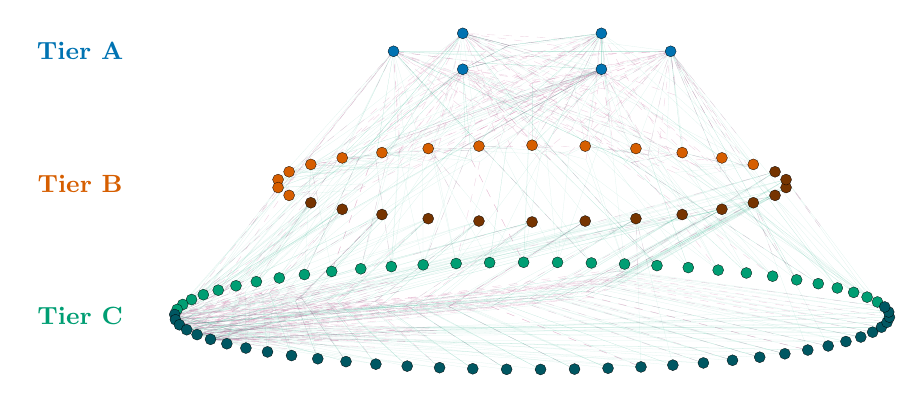
\begin{tikzpicture}[scale=1.4]
  \definecolor{slotin}{rgb}{0.000,0.620,0.450}
  \definecolor{slotout}{rgb}{0.800,0.470,0.650}
  \draw[slotin, line width=0.10pt, opacity=0.12] (1.257,1.200) -- (0.419,1.309);
  \draw[slotin, line width=0.10pt, opacity=0.12] (0.629,1.363) -- (0.419,1.309);
  \draw[slotout, line width=0.14pt, opacity=0.32, dashed] (0.419,1.309) -- (-0.629,1.363);
  \draw[slotin, line width=0.10pt, opacity=0.12] (1.257,1.200) -- (-0.000,1.200);
  \draw[slotin, line width=0.10pt, opacity=0.12] (-0.629,1.363) -- (-0.000,1.200);
  \draw[slotout, line width=0.14pt, opacity=0.32, dashed] (-0.000,1.200) -- (-0.629,1.037);
  \draw[slotin, line width=0.10pt, opacity=0.12] (1.257,1.200) -- (-0.000,1.200);
  \draw[slotin, line width=0.10pt, opacity=0.12] (-0.629,1.037) -- (-0.000,1.200);
  \draw[slotout, line width=0.14pt, opacity=0.32, dashed] (-0.000,1.200) -- (-0.629,1.363);
  \draw[slotin, line width=0.10pt, opacity=0.12] (1.257,1.200) -- (1.507,0.858);
  \draw[slotin, line width=0.10pt, opacity=0.12] (2.007,0.174) -- (1.507,0.858);
  \draw[slotout, line width=0.14pt, opacity=0.32, dashed] (1.507,0.858) -- (1.257,1.200);
  \draw[slotin, line width=0.10pt, opacity=0.12] (1.257,1.200) -- (1.412,0.878);
  \draw[slotin, line width=0.10pt, opacity=0.12] (1.722,0.233) -- (1.412,0.878);
  \draw[slotout, line width=0.14pt, opacity=0.32, dashed] (1.412,0.878) -- (1.257,1.200);
  \draw[slotin, line width=0.10pt, opacity=0.12] (1.257,1.200) -- (1.292,0.894);
  \draw[slotin, line width=0.10pt, opacity=0.12] (1.362,0.281) -- (1.292,0.894);
  \draw[slotout, line width=0.14pt, opacity=0.32, dashed] (1.292,0.894) -- (1.257,1.200);
  \draw[slotin, line width=0.10pt, opacity=0.12] (1.257,1.200) -- (1.152,0.906);
  \draw[slotin, line width=0.10pt, opacity=0.12] (0.942,0.318) -- (1.152,0.906);
  \draw[slotout, line width=0.14pt, opacity=0.32, dashed] (1.152,0.906) -- (1.257,1.200);
  \draw[slotin, line width=0.10pt, opacity=0.12] (1.257,1.200) -- (0.999,0.913);
  \draw[slotin, line width=0.10pt, opacity=0.12] (0.482,0.340) -- (0.999,0.913);
  \draw[slotout, line width=0.14pt, opacity=0.32, dashed] (0.999,0.913) -- (1.257,1.200);
  \draw[slotin, line width=0.10pt, opacity=0.12] (1.257,1.200) -- (1.851,0.457);
  \draw[slotin, line width=0.10pt, opacity=0.12] (3.039,-1.030) -- (1.851,0.457);
  \draw[slotout, line width=0.14pt, opacity=0.32, dashed] (1.851,0.457) -- (1.257,1.200);
  \draw[slotin, line width=0.10pt, opacity=0.12] (1.257,1.200) -- (1.761,0.484);
  \draw[slotin, line width=0.10pt, opacity=0.12] (2.769,-0.947) -- (1.761,0.484);
  \draw[slotout, line width=0.14pt, opacity=0.32, dashed] (1.761,0.484) -- (1.257,1.200);
  \draw[slotin, line width=0.10pt, opacity=0.12] (1.257,1.200) -- (1.638,0.509);
  \draw[slotin, line width=0.10pt, opacity=0.12] (2.400,-0.873) -- (1.638,0.509);
  \draw[slotout, line width=0.14pt, opacity=0.32, dashed] (1.638,0.509) -- (1.257,1.200);
  \draw[slotin, line width=0.10pt, opacity=0.12] (1.257,1.200) -- (1.673,0.203);
  \draw[slotin, line width=0.10pt, opacity=0.12] (2.400,-0.873) -- (1.673,0.203);
  \draw[slotout, line width=0.14pt, opacity=0.32, dashed] (1.673,0.203) -- (1.362,0.281);
  \draw[slotin, line width=0.10pt, opacity=0.12] (1.257,1.200) -- (1.381,0.236);
  \draw[slotin, line width=0.10pt, opacity=0.12] (1.944,-0.811) -- (1.381,0.236);
  \draw[slotout, line width=0.14pt, opacity=0.32, dashed] (1.381,0.236) -- (0.942,0.318);
  \draw[slotin, line width=0.10pt, opacity=0.12] (1.257,1.200) -- (1.052,0.259);
  \draw[slotin, line width=0.10pt, opacity=0.12] (1.417,-0.762) -- (1.052,0.259);
  \draw[slotout, line width=0.14pt, opacity=0.32, dashed] (1.052,0.259) -- (0.482,0.340);
  \draw[slotin, line width=0.10pt, opacity=0.12] (0.629,1.363) -- (-0.210,1.254);
  \draw[slotin, line width=0.10pt, opacity=0.12] (-0.629,1.363) -- (-0.210,1.254);
  \draw[slotout, line width=0.14pt, opacity=0.32, dashed] (-0.210,1.254) -- (-0.629,1.037);
  \draw[slotin, line width=0.10pt, opacity=0.12] (0.629,1.363) -- (-0.210,1.254);
  \draw[slotin, line width=0.10pt, opacity=0.12] (-0.629,1.037) -- (-0.210,1.254);
  \draw[slotout, line width=0.14pt, opacity=0.32, dashed] (-0.210,1.254) -- (-0.629,1.363);
  \draw[slotin, line width=0.10pt, opacity=0.12] (0.629,1.363) -- (1.298,0.912);
  \draw[slotin, line width=0.10pt, opacity=0.12] (2.007,0.174) -- (1.298,0.912);
  \draw[slotout, line width=0.14pt, opacity=0.32, dashed] (1.298,0.912) -- (1.257,1.200);
  \draw[slotin, line width=0.10pt, opacity=0.12] (0.629,1.363) -- (0.629,0.970);
  \draw[slotin, line width=0.10pt, opacity=0.12] (0.000,0.348) -- (0.629,0.970);
  \draw[slotout, line width=0.14pt, opacity=0.32, dashed] (0.629,0.970) -- (1.257,1.200);
  \draw[slotin, line width=0.10pt, opacity=0.12] (0.629,1.363) -- (0.468,0.968);
  \draw[slotin, line width=0.10pt, opacity=0.12] (-0.482,0.340) -- (0.468,0.968);
  \draw[slotout, line width=0.14pt, opacity=0.32, dashed] (0.468,0.968) -- (1.257,1.200);
  \draw[slotin, line width=0.10pt, opacity=0.12] (0.629,1.363) -- (0.315,0.960);
  \draw[slotin, line width=0.10pt, opacity=0.12] (-0.942,0.318) -- (0.315,0.960);
  \draw[slotout, line width=0.14pt, opacity=0.32, dashed] (0.315,0.960) -- (1.257,1.200);
  \draw[slotin, line width=0.10pt, opacity=0.12] (0.629,1.363) -- (0.175,0.948);
  \draw[slotin, line width=0.10pt, opacity=0.12] (-1.362,0.281) -- (0.175,0.948);
  \draw[slotout, line width=0.14pt, opacity=0.32, dashed] (0.175,0.948) -- (1.257,1.200);
  \draw[slotin, line width=0.10pt, opacity=0.12] (0.629,1.363) -- (-0.574,0.303);
  \draw[slotin, line width=0.10pt, opacity=0.12] (-1.362,0.281) -- (-0.574,0.303);
  \draw[slotout, line width=0.14pt, opacity=0.32, dashed] (-0.574,0.303) -- (-0.988,-0.737);
  \draw[slotin, line width=0.10pt, opacity=0.12] (0.629,1.363) -- (1.923,0.154);
  \draw[slotin, line width=0.10pt, opacity=0.12] (3.133,-1.074) -- (1.923,0.154);
  \draw[slotout, line width=0.14pt, opacity=0.32, dashed] (1.923,0.154) -- (2.007,0.174);
  \draw[slotin, line width=0.10pt, opacity=0.12] (0.629,1.363) -- (0.489,0.327);
  \draw[slotin, line width=0.10pt, opacity=0.12] (0.839,-0.730) -- (0.489,0.327);
  \draw[slotout, line width=0.14pt, opacity=0.32, dashed] (0.489,0.327) -- (0.000,0.348);
  \draw[slotin, line width=0.10pt, opacity=0.12] (0.629,1.363) -- (0.126,0.330);
  \draw[slotin, line width=0.10pt, opacity=0.12] (0.231,-0.715) -- (0.126,0.330);
  \draw[slotout, line width=0.14pt, opacity=0.32, dashed] (0.126,0.330) -- (-0.482,0.340);
  \draw[slotin, line width=0.10pt, opacity=0.12] (0.629,1.363) -- (-0.233,0.321);
  \draw[slotin, line width=0.10pt, opacity=0.12] (-0.385,-0.717) -- (-0.233,0.321);
  \draw[slotout, line width=0.14pt, opacity=0.32, dashed] (-0.233,0.321) -- (-0.942,0.318);
  \draw[slotin, line width=0.10pt, opacity=0.12] (0.629,1.363) -- (-0.574,0.303);
  \draw[slotin, line width=0.10pt, opacity=0.12] (-0.988,-0.737) -- (-0.574,0.303);
  \draw[slotout, line width=0.14pt, opacity=0.32, dashed] (-0.574,0.303) -- (-1.362,0.281);
  \draw[slotin, line width=0.10pt, opacity=0.12] (-0.629,1.363) -- (-0.210,1.254);
  \draw[slotin, line width=0.10pt, opacity=0.12] (0.629,1.363) -- (-0.210,1.254);
  \draw[slotout, line width=0.14pt, opacity=0.32, dashed] (-0.210,1.254) -- (-0.629,1.037);
  \draw[slotin, line width=0.10pt, opacity=0.12] (-0.629,1.363) -- (-0.210,1.254);
  \draw[slotin, line width=0.10pt, opacity=0.12] (-0.629,1.037) -- (-0.210,1.254);
  \draw[slotout, line width=0.14pt, opacity=0.32, dashed] (-0.210,1.254) -- (0.629,1.363);
  \draw[slotin, line width=0.10pt, opacity=0.12] (-0.629,1.363) -- (0.784,0.932);
  \draw[slotin, line width=0.10pt, opacity=0.12] (1.722,0.233) -- (0.784,0.932);
  \draw[slotout, line width=0.14pt, opacity=0.32, dashed] (0.784,0.932) -- (1.257,1.200);
  \draw[slotin, line width=0.10pt, opacity=0.12] (-0.629,1.363) -- (0.210,0.970);
  \draw[slotin, line width=0.10pt, opacity=0.12] (0.000,0.348) -- (0.210,0.970);
  \draw[slotout, line width=0.14pt, opacity=0.32, dashed] (0.210,0.970) -- (1.257,1.200);
  \draw[slotin, line width=0.10pt, opacity=0.12] (-0.629,1.363) -- (0.168,0.322);
  \draw[slotin, line width=0.10pt, opacity=0.12] (0.000,0.348) -- (0.168,0.322);
  \draw[slotout, line width=0.14pt, opacity=0.32, dashed] (0.168,0.322) -- (1.133,-0.744);
  \draw[slotin, line width=0.10pt, opacity=0.12] (-0.629,1.363) -- (-1.302,0.274);
  \draw[slotin, line width=0.10pt, opacity=0.12] (-1.722,0.233) -- (-1.302,0.274);
  \draw[slotout, line width=0.14pt, opacity=0.32, dashed] (-1.302,0.274) -- (-1.554,-0.773);
  \draw[slotin, line width=0.10pt, opacity=0.12] (-0.629,1.363) -- (-1.567,0.237);
  \draw[slotin, line width=0.10pt, opacity=0.12] (-2.007,0.174) -- (-1.567,0.237);
  \draw[slotout, line width=0.14pt, opacity=0.32, dashed] (-1.567,0.237) -- (-2.065,-0.825);
  \draw[slotin, line width=0.10pt, opacity=0.12] (-0.629,1.363) -- (-1.778,0.193);
  \draw[slotin, line width=0.10pt, opacity=0.12] (-2.204,0.107) -- (-1.778,0.193);
  \draw[slotout, line width=0.14pt, opacity=0.32, dashed] (-1.778,0.193) -- (-2.501,-0.890);
  \draw[slotin, line width=0.10pt, opacity=0.12] (-0.629,1.363) -- (1.337,0.203);
  \draw[slotin, line width=0.10pt, opacity=0.12] (2.917,-0.987) -- (1.337,0.203);
  \draw[slotout, line width=0.14pt, opacity=0.32, dashed] (1.337,0.203) -- (1.722,0.233);
  \draw[slotin, line width=0.10pt, opacity=0.12] (-0.629,1.363) -- (0.168,0.322);
  \draw[slotin, line width=0.10pt, opacity=0.12] (1.133,-0.744) -- (0.168,0.322);
  \draw[slotout, line width=0.14pt, opacity=0.32, dashed] (0.168,0.322) -- (0.000,0.348);
  \draw[slotin, line width=0.10pt, opacity=0.12] (-0.629,1.363) -- (-1.302,0.274);
  \draw[slotin, line width=0.10pt, opacity=0.12] (-1.554,-0.773) -- (-1.302,0.274);
  \draw[slotout, line width=0.14pt, opacity=0.32, dashed] (-1.302,0.274) -- (-1.722,0.233);
  \draw[slotin, line width=0.10pt, opacity=0.12] (-0.629,1.363) -- (-1.567,0.237);
  \draw[slotin, line width=0.10pt, opacity=0.12] (-2.065,-0.825) -- (-1.567,0.237);
  \draw[slotout, line width=0.14pt, opacity=0.32, dashed] (-1.567,0.237) -- (-2.007,0.174);
  \draw[slotin, line width=0.10pt, opacity=0.12] (-0.629,1.363) -- (-1.778,0.193);
  \draw[slotin, line width=0.10pt, opacity=0.12] (-2.501,-0.890) -- (-1.778,0.193);
  \draw[slotout, line width=0.14pt, opacity=0.32, dashed] (-1.778,0.193) -- (-2.204,0.107);
  \draw[slotin, line width=0.10pt, opacity=0.12] (-1.257,1.200) -- (-0.419,1.200);
  \draw[slotin, line width=0.10pt, opacity=0.12] (0.629,1.363) -- (-0.419,1.200);
  \draw[slotout, line width=0.14pt, opacity=0.32, dashed] (-0.419,1.200) -- (-0.629,1.037);
  \draw[slotin, line width=0.10pt, opacity=0.12] (-1.257,1.200) -- (-0.210,1.146);
  \draw[slotin, line width=0.10pt, opacity=0.12] (-0.629,1.037) -- (-0.210,1.146);
  \draw[slotout, line width=0.14pt, opacity=0.32, dashed] (-0.210,1.146) -- (1.257,1.200);
  \draw[slotin, line width=0.10pt, opacity=0.12] (-1.257,1.200) -- (-0.419,1.091);
  \draw[slotin, line width=0.10pt, opacity=0.12] (0.629,1.037) -- (-0.419,1.091);
  \draw[slotout, line width=0.14pt, opacity=0.32, dashed] (-0.419,1.091) -- (-0.629,1.037);
  \draw[slotin, line width=0.10pt, opacity=0.12] (-1.257,1.200) -- (0.900,0.191);
  \draw[slotin, line width=0.10pt, opacity=0.12] (1.362,0.281) -- (0.900,0.191);
  \draw[slotout, line width=0.14pt, opacity=0.32, dashed] (0.900,0.191) -- (2.596,-0.908);
  \draw[slotin, line width=0.10pt, opacity=0.12] (-1.257,1.200) -- (-0.400,0.273);
  \draw[slotin, line width=0.10pt, opacity=0.12] (-0.482,0.340) -- (-0.400,0.273);
  \draw[slotout, line width=0.14pt, opacity=0.32, dashed] (-0.400,0.273) -- (0.538,-0.720);
  \draw[slotin, line width=0.10pt, opacity=0.12] (-1.257,1.200) -- (-1.419,0.227);
  \draw[slotin, line width=0.10pt, opacity=0.12] (-1.722,0.233) -- (-1.419,0.227);
  \draw[slotout, line width=0.14pt, opacity=0.32, dashed] (-1.419,0.227) -- (-1.277,-0.753);
  \draw[slotin, line width=0.10pt, opacity=0.12] (-1.257,1.200) -- (-2.136,0.090);
  \draw[slotin, line width=0.10pt, opacity=0.12] (-2.304,0.036) -- (-2.136,0.090);
  \draw[slotout, line width=0.14pt, opacity=0.32, dashed] (-2.136,0.090) -- (-2.847,-0.967);
  \draw[slotin, line width=0.10pt, opacity=0.12] (-1.257,1.200) -- (-2.217,0.037);
  \draw[slotin, line width=0.10pt, opacity=0.12] (-2.304,-0.036) -- (-2.217,0.037);
  \draw[slotout, line width=0.14pt, opacity=0.32, dashed] (-2.217,0.037) -- (-3.089,-1.052);
  \draw[slotin, line width=0.10pt, opacity=0.12] (-1.257,1.200) -- (0.900,0.191);
  \draw[slotin, line width=0.10pt, opacity=0.12] (2.596,-0.908) -- (0.900,0.191);
  \draw[slotout, line width=0.14pt, opacity=0.32, dashed] (0.900,0.191) -- (1.362,0.281);
  \draw[slotin, line width=0.10pt, opacity=0.12] (-1.257,1.200) -- (-0.400,0.273);
  \draw[slotin, line width=0.10pt, opacity=0.12] (0.538,-0.720) -- (-0.400,0.273);
  \draw[slotout, line width=0.14pt, opacity=0.32, dashed] (-0.400,0.273) -- (-0.482,0.340);
  \draw[slotin, line width=0.10pt, opacity=0.12] (-1.257,1.200) -- (-1.419,0.227);
  \draw[slotin, line width=0.10pt, opacity=0.12] (-1.277,-0.753) -- (-1.419,0.227);
  \draw[slotout, line width=0.14pt, opacity=0.32, dashed] (-1.419,0.227) -- (-1.722,0.233);
  \draw[slotin, line width=0.10pt, opacity=0.12] (-1.257,1.200) -- (-1.158,0.423);
  \draw[slotin, line width=0.10pt, opacity=0.12] (-2.847,-0.967) -- (-1.158,0.423);
  \draw[slotout, line width=0.14pt, opacity=0.32, dashed] (-1.158,0.423) -- (0.629,1.037);
  \draw[slotin, line width=0.10pt, opacity=0.12] (-1.257,1.200) -- (-1.239,0.395);
  \draw[slotin, line width=0.10pt, opacity=0.12] (-3.089,-1.052) -- (-1.239,0.395);
  \draw[slotout, line width=0.14pt, opacity=0.32, dashed] (-1.239,0.395) -- (0.629,1.037);
  \draw[slotin, line width=0.10pt, opacity=0.12] (-0.629,1.037) -- (-0.210,1.254);
  \draw[slotin, line width=0.10pt, opacity=0.12] (0.629,1.363) -- (-0.210,1.254);
  \draw[slotout, line width=0.14pt, opacity=0.32, dashed] (-0.210,1.254) -- (-0.629,1.363);
  \draw[slotin, line width=0.10pt, opacity=0.12] (-0.629,1.037) -- (-0.210,1.146);
  \draw[slotin, line width=0.10pt, opacity=0.12] (-1.257,1.200) -- (-0.210,1.146);
  \draw[slotout, line width=0.14pt, opacity=0.32, dashed] (-0.210,1.146) -- (1.257,1.200);
  \draw[slotin, line width=0.10pt, opacity=0.12] (-0.629,1.037) -- (-0.419,1.091);
  \draw[slotin, line width=0.10pt, opacity=0.12] (0.629,1.037) -- (-0.419,1.091);
  \draw[slotout, line width=0.14pt, opacity=0.32, dashed] (-0.419,1.091) -- (-1.257,1.200);
  \draw[slotin, line width=0.10pt, opacity=0.12] (-0.629,1.037) -- (0.832,0.171);
  \draw[slotin, line width=0.10pt, opacity=0.12] (0.942,0.318) -- (0.832,0.171);
  \draw[slotout, line width=0.14pt, opacity=0.32, dashed] (0.832,0.171) -- (2.182,-0.840);
  \draw[slotin, line width=0.10pt, opacity=0.12] (-0.629,1.037) -- (-0.549,0.214);
  \draw[slotin, line width=0.10pt, opacity=0.12] (-0.942,0.318) -- (-0.549,0.214);
  \draw[slotout, line width=0.14pt, opacity=0.32, dashed] (-0.549,0.214) -- (-0.077,-0.714);
  \draw[slotin, line width=0.10pt, opacity=0.12] (-0.629,1.037) -- (-1.484,0.138);
  \draw[slotin, line width=0.10pt, opacity=0.12] (-2.007,0.174) -- (-1.484,0.138);
  \draw[slotout, line width=0.14pt, opacity=0.32, dashed] (-1.484,0.138) -- (-1.818,-0.797);
  \draw[slotin, line width=0.10pt, opacity=0.12] (-0.629,1.037) -- (-1.873,0.049);
  \draw[slotin, line width=0.10pt, opacity=0.12] (-2.304,0.036) -- (-1.873,0.049);
  \draw[slotout, line width=0.14pt, opacity=0.32, dashed] (-1.873,0.049) -- (-2.686,-0.927);
  \draw[slotin, line width=0.10pt, opacity=0.12] (-0.629,1.037) -- (-2.018,-0.071);
  \draw[slotin, line width=0.10pt, opacity=0.12] (-2.204,-0.107) -- (-2.018,-0.071);
  \draw[slotout, line width=0.14pt, opacity=0.32, dashed] (-2.018,-0.071) -- (-3.220,-1.142);
  \draw[slotin, line width=0.10pt, opacity=0.12] (-0.629,1.037) -- (0.727,0.411);
  \draw[slotin, line width=0.10pt, opacity=0.12] (2.182,-0.840) -- (0.727,0.411);
  \draw[slotout, line width=0.14pt, opacity=0.32, dashed] (0.727,0.411) -- (0.629,1.037);
  \draw[slotin, line width=0.10pt, opacity=0.12] (-0.629,1.037) -- (-0.026,0.453);
  \draw[slotin, line width=0.10pt, opacity=0.12] (-0.077,-0.714) -- (-0.026,0.453);
  \draw[slotout, line width=0.14pt, opacity=0.32, dashed] (-0.026,0.453) -- (0.629,1.037);
  \draw[slotin, line width=0.10pt, opacity=0.12] (-0.629,1.037) -- (-0.606,0.425);
  \draw[slotin, line width=0.10pt, opacity=0.12] (-1.818,-0.797) -- (-0.606,0.425);
  \draw[slotout, line width=0.14pt, opacity=0.32, dashed] (-0.606,0.425) -- (0.629,1.037);
  \draw[slotin, line width=0.10pt, opacity=0.12] (-0.629,1.037) -- (-0.895,0.382);
  \draw[slotin, line width=0.10pt, opacity=0.12] (-2.686,-0.927) -- (-0.895,0.382);
  \draw[slotout, line width=0.14pt, opacity=0.32, dashed] (-0.895,0.382) -- (0.629,1.037);
  \draw[slotin, line width=0.10pt, opacity=0.12] (-0.629,1.037) -- (-1.073,0.310);
  \draw[slotin, line width=0.10pt, opacity=0.12] (-3.220,-1.142) -- (-1.073,0.310);
  \draw[slotout, line width=0.14pt, opacity=0.32, dashed] (-1.073,0.310) -- (0.629,1.037);
  \draw[slotin, line width=0.10pt, opacity=0.12] (0.629,1.037) -- (0.210,1.254);
  \draw[slotin, line width=0.10pt, opacity=0.12] (0.629,1.363) -- (0.210,1.254);
  \draw[slotout, line width=0.14pt, opacity=0.32, dashed] (0.210,1.254) -- (-0.629,1.363);
  \draw[slotin, line width=0.10pt, opacity=0.12] (0.629,1.037) -- (0.210,1.146);
  \draw[slotin, line width=0.10pt, opacity=0.12] (-1.257,1.200) -- (0.210,1.146);
  \draw[slotout, line width=0.14pt, opacity=0.32, dashed] (0.210,1.146) -- (1.257,1.200);
  \draw[slotin, line width=0.10pt, opacity=0.12] (0.629,1.037) -- (-0.419,1.091);
  \draw[slotin, line width=0.10pt, opacity=0.12] (-0.629,1.037) -- (-0.419,1.091);
  \draw[slotout, line width=0.14pt, opacity=0.32, dashed] (-0.419,1.091) -- (-1.257,1.200);
  \draw[slotin, line width=0.10pt, opacity=0.12] (0.629,1.037) -- (0.933,0.197);
  \draw[slotin, line width=0.10pt, opacity=0.12] (0.482,0.340) -- (0.933,0.197);
  \draw[slotout, line width=0.14pt, opacity=0.32, dashed] (0.933,0.197) -- (1.688,-0.785);
  \draw[slotin, line width=0.10pt, opacity=0.12] (0.629,1.037) -- (-0.474,0.198);
  \draw[slotin, line width=0.10pt, opacity=0.12] (-1.362,0.281) -- (-0.474,0.198);
  \draw[slotout, line width=0.14pt, opacity=0.32, dashed] (-0.474,0.198) -- (-0.689,-0.725);
  \draw[slotin, line width=0.10pt, opacity=0.12] (0.629,1.037) -- (-0.315,0.727);
  \draw[slotin, line width=0.10pt, opacity=0.12] (-2.204,0.107) -- (-0.315,0.727);
  \draw[slotout, line width=0.14pt, opacity=0.32, dashed] (-0.315,0.727) -- (0.629,1.037);
  \draw[slotin, line width=0.10pt, opacity=0.12] (0.629,1.037) -- (-0.349,0.679);
  \draw[slotin, line width=0.10pt, opacity=0.12] (-2.304,-0.036) -- (-0.349,0.679);
  \draw[slotout, line width=0.14pt, opacity=0.32, dashed] (-0.349,0.679) -- (0.629,1.037);
  \draw[slotin, line width=0.10pt, opacity=0.12] (0.629,1.037) -- (-0.315,0.655);
  \draw[slotin, line width=0.10pt, opacity=0.12] (-2.204,-0.107) -- (-0.315,0.655);
  \draw[slotout, line width=0.14pt, opacity=0.32, dashed] (-0.315,0.655) -- (0.629,1.037);
  \draw[slotin, line width=0.10pt, opacity=0.12] (0.629,1.037) -- (0.982,0.430);
  \draw[slotin, line width=0.10pt, opacity=0.12] (1.688,-0.785) -- (0.982,0.430);
  \draw[slotout, line width=0.14pt, opacity=0.32, dashed] (0.982,0.430) -- (0.629,1.037);
  \draw[slotin, line width=0.10pt, opacity=0.12] (0.629,1.037) -- (0.189,0.450);
  \draw[slotin, line width=0.10pt, opacity=0.12] (-0.689,-0.725) -- (0.189,0.450);
  \draw[slotout, line width=0.14pt, opacity=0.32, dashed] (0.189,0.450) -- (0.629,1.037);
  \draw[slotin, line width=0.10pt, opacity=0.12] (0.629,1.037) -- (-0.345,0.406);
  \draw[slotin, line width=0.10pt, opacity=0.12] (-2.293,-0.856) -- (-0.345,0.406);
  \draw[slotout, line width=0.14pt, opacity=0.32, dashed] (-0.345,0.406) -- (0.629,1.037);
  \draw[slotin, line width=0.10pt, opacity=0.12] (0.629,1.037) -- (-0.575,0.355);
  \draw[slotin, line width=0.10pt, opacity=0.12] (-2.982,-1.008) -- (-0.575,0.355);
  \draw[slotout, line width=0.14pt, opacity=0.32, dashed] (-0.575,0.355) -- (0.629,1.037);
  \draw[slotin, line width=0.10pt, opacity=0.12] (0.629,1.037) -- (-0.637,0.326);
  \draw[slotin, line width=0.10pt, opacity=0.12] (-3.169,-1.097) -- (-0.637,0.326);
  \draw[slotout, line width=0.14pt, opacity=0.32, dashed] (-0.637,0.326) -- (0.629,1.037);
  \draw[slotin, line width=0.10pt, opacity=0.12] (2.007,0.174) -- (1.298,0.803);
  \draw[slotin, line width=0.10pt, opacity=0.12] (1.257,1.200) -- (1.298,0.803);
  \draw[slotout, line width=0.14pt, opacity=0.32, dashed] (1.298,0.803) -- (0.629,1.037);
  \draw[slotin, line width=0.10pt, opacity=0.12] (2.007,0.174) -- (0.669,0.858);
  \draw[slotin, line width=0.10pt, opacity=0.12] (0.629,1.363) -- (0.669,0.858);
  \draw[slotout, line width=0.14pt, opacity=0.32, dashed] (0.669,0.858) -- (-0.629,1.037);
  \draw[slotin, line width=0.10pt, opacity=0.12] (2.007,0.174) -- (1.504,0.154);
  \draw[slotin, line width=0.10pt, opacity=0.12] (3.133,-1.074) -- (1.504,0.154);
  \draw[slotout, line width=0.14pt, opacity=0.32, dashed] (1.504,0.154) -- (-0.629,1.363);
  \draw[slotin, line width=0.10pt, opacity=0.12] (2.007,0.174) -- (1.472,0.169);
  \draw[slotin, line width=0.10pt, opacity=0.12] (3.039,-1.030) -- (1.472,0.169);
  \draw[slotout, line width=0.14pt, opacity=0.32, dashed] (1.472,0.169) -- (-0.629,1.363);
  \draw[slotin, line width=0.10pt, opacity=0.12] (1.722,0.233) -- (0.784,0.932);
  \draw[slotin, line width=0.10pt, opacity=0.12] (1.257,1.200) -- (0.784,0.932);
  \draw[slotout, line width=0.14pt, opacity=0.32, dashed] (0.784,0.932) -- (-0.629,1.363);
  \draw[slotin, line width=0.10pt, opacity=0.12] (1.722,0.233) -- (0.574,0.986);
  \draw[slotin, line width=0.10pt, opacity=0.12] (-0.629,1.363) -- (0.574,0.986);
  \draw[slotout, line width=0.14pt, opacity=0.32, dashed] (0.574,0.986) -- (0.629,1.363);
  \draw[slotin, line width=0.10pt, opacity=0.12] (1.722,0.233) -- (1.966,0.148);
  \draw[slotin, line width=0.10pt, opacity=0.12] (2.917,-0.987) -- (1.966,0.148);
  \draw[slotout, line width=0.14pt, opacity=0.32, dashed] (1.966,0.148) -- (1.257,1.200);
  \draw[slotin, line width=0.10pt, opacity=0.12] (1.722,0.233) -- (1.916,0.162);
  \draw[slotin, line width=0.10pt, opacity=0.12] (2.769,-0.947) -- (1.916,0.162);
  \draw[slotout, line width=0.14pt, opacity=0.32, dashed] (1.916,0.162) -- (1.257,1.200);
  \draw[slotin, line width=0.10pt, opacity=0.12] (1.362,0.281) -- (1.292,0.894);
  \draw[slotin, line width=0.10pt, opacity=0.12] (1.257,1.200) -- (1.292,0.894);
  \draw[slotout, line width=0.14pt, opacity=0.32, dashed] (1.292,0.894) -- (1.257,1.200);
  \draw[slotin, line width=0.10pt, opacity=0.12] (1.362,0.281) -- (1.673,0.203);
  \draw[slotin, line width=0.10pt, opacity=0.12] (1.257,1.200) -- (1.673,0.203);
  \draw[slotout, line width=0.14pt, opacity=0.32, dashed] (1.673,0.203) -- (2.400,-0.873);
  \draw[slotin, line width=0.10pt, opacity=0.12] (1.362,0.281) -- (0.489,0.587);
  \draw[slotin, line width=0.10pt, opacity=0.12] (-1.257,1.200) -- (0.489,0.587);
  \draw[slotout, line width=0.14pt, opacity=0.32, dashed] (0.489,0.587) -- (1.362,0.281);
  \draw[slotin, line width=0.10pt, opacity=0.12] (1.362,0.281) -- (1.529,0.136);
  \draw[slotin, line width=0.10pt, opacity=0.12] (2.596,-0.908) -- (1.529,0.136);
  \draw[slotout, line width=0.14pt, opacity=0.32, dashed] (1.529,0.136) -- (0.629,1.037);
  \draw[slotin, line width=0.10pt, opacity=0.12] (1.362,0.281) -- (1.044,0.148);
  \draw[slotin, line width=0.10pt, opacity=0.12] (2.400,-0.873) -- (1.044,0.148);
  \draw[slotout, line width=0.14pt, opacity=0.32, dashed] (1.044,0.148) -- (-0.629,1.037);
  \draw[slotin, line width=0.10pt, opacity=0.12] (0.942,0.318) -- (0.524,0.851);
  \draw[slotin, line width=0.10pt, opacity=0.12] (1.257,1.200) -- (0.524,0.851);
  \draw[slotout, line width=0.14pt, opacity=0.32, dashed] (0.524,0.851) -- (-0.629,1.037);
  \draw[slotin, line width=0.10pt, opacity=0.12] (0.942,0.318) -- (-0.315,0.851);
  \draw[slotin, line width=0.10pt, opacity=0.12] (-0.629,1.037) -- (-0.315,0.851);
  \draw[slotout, line width=0.14pt, opacity=0.32, dashed] (-0.315,0.851) -- (-1.257,1.200);
  \draw[slotin, line width=0.10pt, opacity=0.12] (0.942,0.318) -- (0.832,0.280);
  \draw[slotin, line width=0.10pt, opacity=0.12] (2.182,-0.840) -- (0.832,0.280);
  \draw[slotout, line width=0.14pt, opacity=0.32, dashed] (0.832,0.280) -- (-0.629,1.363);
  \draw[slotin, line width=0.10pt, opacity=0.12] (0.942,0.318) -- (0.752,0.290);
  \draw[slotin, line width=0.10pt, opacity=0.12] (1.944,-0.811) -- (0.752,0.290);
  \draw[slotout, line width=0.14pt, opacity=0.32, dashed] (0.752,0.290) -- (-0.629,1.363);
  \draw[slotin, line width=0.10pt, opacity=0.12] (0.482,0.340) -- (0.370,0.968);
  \draw[slotin, line width=0.10pt, opacity=0.12] (1.257,1.200) -- (0.370,0.968);
  \draw[slotout, line width=0.14pt, opacity=0.32, dashed] (0.370,0.968) -- (-0.629,1.363);
  \draw[slotin, line width=0.10pt, opacity=0.12] (0.482,0.340) -- (0.580,0.913);
  \draw[slotin, line width=0.10pt, opacity=0.12] (0.629,1.037) -- (0.580,0.913);
  \draw[slotout, line width=0.14pt, opacity=0.32, dashed] (0.580,0.913) -- (0.629,1.363);
  \draw[slotin, line width=0.10pt, opacity=0.12] (0.482,0.340) -- (1.142,0.252);
  \draw[slotin, line width=0.10pt, opacity=0.12] (1.688,-0.785) -- (1.142,0.252);
  \draw[slotout, line width=0.14pt, opacity=0.32, dashed] (1.142,0.252) -- (1.257,1.200);
  \draw[slotin, line width=0.10pt, opacity=0.12] (0.482,0.340) -- (1.052,0.259);
  \draw[slotin, line width=0.10pt, opacity=0.12] (1.417,-0.762) -- (1.052,0.259);
  \draw[slotout, line width=0.14pt, opacity=0.32, dashed] (1.052,0.259) -- (1.257,1.200);
  \draw[slotin, line width=0.10pt, opacity=0.12] (0.000,0.348) -- (0.629,0.970);
  \draw[slotin, line width=0.10pt, opacity=0.12] (0.629,1.363) -- (0.629,0.970);
  \draw[slotout, line width=0.14pt, opacity=0.32, dashed] (0.629,0.970) -- (1.257,1.200);
  \draw[slotin, line width=0.10pt, opacity=0.12] (0.000,0.348) -- (0.210,0.686);
  \draw[slotin, line width=0.10pt, opacity=0.12] (0.629,1.363) -- (0.210,0.686);
  \draw[slotout, line width=0.14pt, opacity=0.32, dashed] (0.210,0.686) -- (0.000,0.348);
  \draw[slotin, line width=0.10pt, opacity=0.12] (0.000,0.348) -- (0.000,0.916);
  \draw[slotin, line width=0.10pt, opacity=0.12] (-0.629,1.363) -- (0.000,0.916);
  \draw[slotout, line width=0.14pt, opacity=0.32, dashed] (0.000,0.916) -- (0.629,1.037);
  \draw[slotin, line width=0.10pt, opacity=0.12] (0.000,0.348) -- (0.168,0.213);
  \draw[slotin, line width=0.10pt, opacity=0.12] (1.133,-0.744) -- (0.168,0.213);
  \draw[slotout, line width=0.14pt, opacity=0.32, dashed] (0.168,0.213) -- (-0.629,1.037);
  \draw[slotin, line width=0.10pt, opacity=0.12] (0.000,0.348) -- (0.070,0.218);
  \draw[slotin, line width=0.10pt, opacity=0.12] (0.839,-0.730) -- (0.070,0.218);
  \draw[slotout, line width=0.14pt, opacity=0.32, dashed] (0.070,0.218) -- (-0.629,1.037);
  \draw[slotin, line width=0.10pt, opacity=0.12] (-0.482,0.340) -- (-0.161,0.913);
  \draw[slotin, line width=0.10pt, opacity=0.12] (0.629,1.363) -- (-0.161,0.913);
  \draw[slotout, line width=0.14pt, opacity=0.32, dashed] (-0.161,0.913) -- (-0.629,1.037);
  \draw[slotin, line width=0.10pt, opacity=0.12] (-0.482,0.340) -- (-0.999,0.913);
  \draw[slotin, line width=0.10pt, opacity=0.12] (-1.257,1.200) -- (-0.999,0.913);
  \draw[slotout, line width=0.14pt, opacity=0.32, dashed] (-0.999,0.913) -- (-1.257,1.200);
  \draw[slotin, line width=0.10pt, opacity=0.12] (-0.482,0.340) -- (-0.191,0.328);
  \draw[slotin, line width=0.10pt, opacity=0.12] (0.538,-0.720) -- (-0.191,0.328);
  \draw[slotout, line width=0.14pt, opacity=0.32, dashed] (-0.191,0.328) -- (-0.629,1.363);
  \draw[slotin, line width=0.10pt, opacity=0.12] (-0.482,0.340) -- (-0.293,0.330);
  \draw[slotin, line width=0.10pt, opacity=0.12] (0.231,-0.715) -- (-0.293,0.330);
  \draw[slotout, line width=0.14pt, opacity=0.32, dashed] (-0.293,0.330) -- (-0.629,1.363);
  \draw[slotin, line width=0.10pt, opacity=0.12] (-0.942,0.318) -- (-0.314,1.015);
  \draw[slotin, line width=0.10pt, opacity=0.12] (0.629,1.363) -- (-0.314,1.015);
  \draw[slotout, line width=0.14pt, opacity=0.32, dashed] (-0.314,1.015) -- (-0.629,1.363);
  \draw[slotin, line width=0.10pt, opacity=0.12] (-0.942,0.318) -- (-0.314,0.906);
  \draw[slotin, line width=0.10pt, opacity=0.12] (-0.629,1.037) -- (-0.314,0.906);
  \draw[slotout, line width=0.14pt, opacity=0.32, dashed] (-0.314,0.906) -- (0.629,1.363);
  \draw[slotin, line width=0.10pt, opacity=0.12] (-0.942,0.318) -- (-0.549,0.214);
  \draw[slotin, line width=0.10pt, opacity=0.12] (-0.629,1.037) -- (-0.549,0.214);
  \draw[slotout, line width=0.14pt, opacity=0.32, dashed] (-0.549,0.214) -- (-0.077,-0.714);
  \draw[slotin, line width=0.10pt, opacity=0.12] (-0.942,0.318) -- (-0.654,-0.026);
  \draw[slotin, line width=0.10pt, opacity=0.12] (-0.077,-0.714) -- (-0.654,-0.026);
  \draw[slotout, line width=0.14pt, opacity=0.32, dashed] (-0.654,-0.026) -- (-0.942,0.318);
  \draw[slotin, line width=0.10pt, opacity=0.12] (-0.942,0.318) -- (-0.757,-0.027);
  \draw[slotin, line width=0.10pt, opacity=0.12] (-0.385,-0.717) -- (-0.757,-0.027);
  \draw[slotout, line width=0.14pt, opacity=0.32, dashed] (-0.757,-0.027) -- (-0.942,0.318);
  \draw[slotin, line width=0.10pt, opacity=0.12] (-1.362,0.281) -- (-0.698,0.642);
  \draw[slotin, line width=0.10pt, opacity=0.12] (0.629,1.363) -- (-0.698,0.642);
  \draw[slotout, line width=0.14pt, opacity=0.32, dashed] (-0.698,0.642) -- (-1.362,0.281);
  \draw[slotin, line width=0.10pt, opacity=0.12] (-1.362,0.281) -- (-0.035,0.785);
  \draw[slotin, line width=0.10pt, opacity=0.12] (0.629,1.037) -- (-0.035,0.785);
  \draw[slotout, line width=0.14pt, opacity=0.32, dashed] (-0.035,0.785) -- (0.629,1.037);
  \draw[slotin, line width=0.10pt, opacity=0.12] (-1.362,0.281) -- (-0.893,0.198);
  \draw[slotin, line width=0.10pt, opacity=0.12] (-0.689,-0.725) -- (-0.893,0.198);
  \draw[slotout, line width=0.14pt, opacity=0.32, dashed] (-0.893,0.198) -- (-0.629,1.037);
  \draw[slotin, line width=0.10pt, opacity=0.12] (-1.362,0.281) -- (-0.993,0.194);
  \draw[slotin, line width=0.10pt, opacity=0.12] (-0.988,-0.737) -- (-0.993,0.194);
  \draw[slotout, line width=0.14pt, opacity=0.32, dashed] (-0.993,0.194) -- (-0.629,1.037);
  \draw[slotin, line width=0.10pt, opacity=0.12] (-1.722,0.233) -- (-0.993,0.878);
  \draw[slotin, line width=0.10pt, opacity=0.12] (-0.629,1.363) -- (-0.993,0.878);
  \draw[slotout, line width=0.14pt, opacity=0.32, dashed] (-0.993,0.878) -- (-0.629,1.037);
  \draw[slotin, line width=0.10pt, opacity=0.12] (-1.722,0.233) -- (-1.412,0.878);
  \draw[slotin, line width=0.10pt, opacity=0.12] (-1.257,1.200) -- (-1.412,0.878);
  \draw[slotout, line width=0.14pt, opacity=0.32, dashed] (-1.412,0.878) -- (-1.257,1.200);
  \draw[slotin, line width=0.10pt, opacity=0.12] (-1.722,0.233) -- (-1.209,0.281);
  \draw[slotin, line width=0.10pt, opacity=0.12] (-1.277,-0.753) -- (-1.209,0.281);
  \draw[slotout, line width=0.14pt, opacity=0.32, dashed] (-1.209,0.281) -- (-0.629,1.363);
  \draw[slotin, line width=0.10pt, opacity=0.12] (-1.722,0.233) -- (-0.883,0.274);
  \draw[slotin, line width=0.10pt, opacity=0.12] (-1.554,-0.773) -- (-0.883,0.274);
  \draw[slotout, line width=0.14pt, opacity=0.32, dashed] (-0.883,0.274) -- (0.629,1.363);
  \draw[slotin, line width=0.10pt, opacity=0.12] (-2.007,0.174) -- (-0.669,0.967);
  \draw[slotin, line width=0.10pt, opacity=0.12] (-0.629,1.363) -- (-0.669,0.967);
  \draw[slotout, line width=0.14pt, opacity=0.32, dashed] (-0.669,0.967) -- (0.629,1.363);
  \draw[slotin, line width=0.10pt, opacity=0.12] (-2.007,0.174) -- (-0.459,0.803);
  \draw[slotin, line width=0.10pt, opacity=0.12] (-0.629,1.037) -- (-0.459,0.803);
  \draw[slotout, line width=0.14pt, opacity=0.32, dashed] (-0.459,0.803) -- (1.257,1.200);
  \draw[slotin, line width=0.10pt, opacity=0.12] (-2.007,0.174) -- (-1.484,0.138);
  \draw[slotin, line width=0.10pt, opacity=0.12] (-0.629,1.037) -- (-1.484,0.138);
  \draw[slotout, line width=0.14pt, opacity=0.32, dashed] (-1.484,0.138) -- (-1.818,-0.797);
  \draw[slotin, line width=0.10pt, opacity=0.12] (-2.007,0.174) -- (-1.944,-0.150);
  \draw[slotin, line width=0.10pt, opacity=0.12] (-1.818,-0.797) -- (-1.944,-0.150);
  \draw[slotout, line width=0.14pt, opacity=0.32, dashed] (-1.944,-0.150) -- (-2.007,0.174);
  \draw[slotin, line width=0.10pt, opacity=0.12] (-2.007,0.174) -- (-2.026,-0.159);
  \draw[slotin, line width=0.10pt, opacity=0.12] (-2.065,-0.825) -- (-2.026,-0.159);
  \draw[slotout, line width=0.14pt, opacity=0.32, dashed] (-2.026,-0.159) -- (-2.007,0.174);
  \draw[slotin, line width=0.10pt, opacity=0.12] (-2.204,0.107) -- (-1.679,0.526);
  \draw[slotin, line width=0.10pt, opacity=0.12] (-0.629,1.363) -- (-1.679,0.526);
  \draw[slotout, line width=0.14pt, opacity=0.32, dashed] (-1.679,0.526) -- (-2.204,0.107);
  \draw[slotin, line width=0.10pt, opacity=0.12] (-2.204,0.107) -- (-0.315,0.727);
  \draw[slotin, line width=0.10pt, opacity=0.12] (0.629,1.037) -- (-0.315,0.727);
  \draw[slotout, line width=0.14pt, opacity=0.32, dashed] (-0.315,0.727) -- (0.629,1.037);
  \draw[slotin, line width=0.10pt, opacity=0.12] (-2.204,0.107) -- (-1.709,0.096);
  \draw[slotin, line width=0.10pt, opacity=0.12] (-2.293,-0.856) -- (-1.709,0.096);
  \draw[slotout, line width=0.14pt, opacity=0.32, dashed] (-1.709,0.096) -- (-0.629,1.037);
  \draw[slotin, line width=0.10pt, opacity=0.12] (-2.204,0.107) -- (-1.778,0.085);
  \draw[slotin, line width=0.10pt, opacity=0.12] (-2.501,-0.890) -- (-1.778,0.085);
  \draw[slotout, line width=0.14pt, opacity=0.32, dashed] (-1.778,0.085) -- (-0.629,1.037);
  \draw[slotin, line width=0.10pt, opacity=0.12] (-2.304,0.036) -- (-1.606,0.812);
  \draw[slotin, line width=0.10pt, opacity=0.12] (-1.257,1.200) -- (-1.606,0.812);
  \draw[slotout, line width=0.14pt, opacity=0.32, dashed] (-1.606,0.812) -- (-1.257,1.200);
  \draw[slotin, line width=0.10pt, opacity=0.12] (-2.304,0.036) -- (-1.187,0.812);
  \draw[slotin, line width=0.10pt, opacity=0.12] (-0.629,1.037) -- (-1.187,0.812);
  \draw[slotout, line width=0.14pt, opacity=0.32, dashed] (-1.187,0.812) -- (-0.629,1.363);
  \draw[slotin, line width=0.10pt, opacity=0.12] (-2.304,0.036) -- (-1.454,0.157);
  \draw[slotin, line width=0.10pt, opacity=0.12] (-2.686,-0.927) -- (-1.454,0.157);
  \draw[slotout, line width=0.14pt, opacity=0.32, dashed] (-1.454,0.157) -- (0.629,1.363);
  \draw[slotin, line width=0.10pt, opacity=0.12] (-2.304,0.036) -- (-1.507,0.144);
  \draw[slotin, line width=0.10pt, opacity=0.12] (-2.847,-0.967) -- (-1.507,0.144);
  \draw[slotout, line width=0.14pt, opacity=0.32, dashed] (-1.507,0.144) -- (0.629,1.363);
  \draw[slotin, line width=0.10pt, opacity=0.12] (-2.304,-0.036) -- (-0.978,0.842);
  \draw[slotin, line width=0.10pt, opacity=0.12] (-1.257,1.200) -- (-0.978,0.842);
  \draw[slotout, line width=0.14pt, opacity=0.32, dashed] (-0.978,0.842) -- (0.629,1.363);
  \draw[slotin, line width=0.10pt, opacity=0.12] (-2.304,-0.036) -- (-0.139,0.733);
  \draw[slotin, line width=0.10pt, opacity=0.12] (0.629,1.037) -- (-0.139,0.733);
  \draw[slotout, line width=0.14pt, opacity=0.32, dashed] (-0.139,0.733) -- (1.257,1.200);
  \draw[slotin, line width=0.10pt, opacity=0.12] (-2.304,-0.036) -- (-1.552,-0.003);
  \draw[slotin, line width=0.10pt, opacity=0.12] (0.629,1.037) -- (-1.552,-0.003);
  \draw[slotout, line width=0.14pt, opacity=0.32, dashed] (-1.552,-0.003) -- (-2.982,-1.008);
  \draw[slotin, line width=0.10pt, opacity=0.12] (-2.304,-0.036) -- (-2.530,-0.360);
  \draw[slotin, line width=0.10pt, opacity=0.12] (-2.982,-1.008) -- (-2.530,-0.360);
  \draw[slotout, line width=0.14pt, opacity=0.32, dashed] (-2.530,-0.360) -- (-2.304,-0.036);
  \draw[slotin, line width=0.10pt, opacity=0.12] (-2.304,-0.036) -- (-2.566,-0.375);
  \draw[slotin, line width=0.10pt, opacity=0.12] (-3.089,-1.052) -- (-2.566,-0.375);
  \draw[slotout, line width=0.14pt, opacity=0.32, dashed] (-2.566,-0.375) -- (-2.304,-0.036);
  \draw[slotin, line width=0.10pt, opacity=0.12] (-2.204,-0.107) -- (-1.679,0.274);
  \draw[slotin, line width=0.10pt, opacity=0.12] (-0.629,1.037) -- (-1.679,0.274);
  \draw[slotout, line width=0.14pt, opacity=0.32, dashed] (-1.679,0.274) -- (-2.204,-0.107);
  \draw[slotin, line width=0.10pt, opacity=0.12] (-2.204,-0.107) -- (-0.735,0.655);
  \draw[slotin, line width=0.10pt, opacity=0.12] (0.629,1.037) -- (-0.735,0.655);
  \draw[slotout, line width=0.14pt, opacity=0.32, dashed] (-0.735,0.655) -- (-0.629,1.037);
  \draw[slotin, line width=0.10pt, opacity=0.12] (-2.204,-0.107) -- (-2.210,-0.001);
  \draw[slotin, line width=0.10pt, opacity=0.12] (-3.169,-1.097) -- (-2.210,-0.001);
  \draw[slotout, line width=0.14pt, opacity=0.32, dashed] (-2.210,-0.001) -- (-1.257,1.200);
  \draw[slotin, line width=0.10pt, opacity=0.12] (-2.204,-0.107) -- (-2.227,-0.017);
  \draw[slotin, line width=0.10pt, opacity=0.12] (-3.220,-1.142) -- (-2.227,-0.017);
  \draw[slotout, line width=0.14pt, opacity=0.32, dashed] (-2.227,-0.017) -- (-1.257,1.200);
  \draw[slotin, line width=0.10pt, opacity=0.12] (3.133,-1.074) -- (0.835,0.496);
  \draw[slotin, line width=0.10pt, opacity=0.12] (0.629,1.363) -- (0.835,0.496);
  \draw[slotout, line width=0.14pt, opacity=0.32, dashed] (0.835,0.496) -- (-1.257,1.200);
  \draw[slotin, line width=0.10pt, opacity=0.12] (3.133,-1.074) -- (1.294,0.100);
  \draw[slotin, line width=0.10pt, opacity=0.12] (2.007,0.174) -- (1.294,0.100);
  \draw[slotout, line width=0.14pt, opacity=0.32, dashed] (1.294,0.100) -- (-1.257,1.200);
  \draw[slotin, line width=0.10pt, opacity=0.12] (3.039,-1.030) -- (1.223,0.402);
  \draw[slotin, line width=0.10pt, opacity=0.12] (1.257,1.200) -- (1.223,0.402);
  \draw[slotout, line width=0.14pt, opacity=0.32, dashed] (1.223,0.402) -- (-0.629,1.037);
  \draw[slotin, line width=0.10pt, opacity=0.12] (3.039,-1.030) -- (1.472,0.060);
  \draw[slotin, line width=0.10pt, opacity=0.12] (2.007,0.174) -- (1.472,0.060);
  \draw[slotout, line width=0.14pt, opacity=0.32, dashed] (1.472,0.060) -- (-0.629,1.037);
  \draw[slotin, line width=0.10pt, opacity=0.12] (2.917,-0.987) -- (0.972,0.471);
  \draw[slotin, line width=0.10pt, opacity=0.12] (-0.629,1.363) -- (0.972,0.471);
  \draw[slotout, line width=0.14pt, opacity=0.32, dashed] (0.972,0.471) -- (0.629,1.037);
  \draw[slotin, line width=0.10pt, opacity=0.12] (2.917,-0.987) -- (1.756,0.094);
  \draw[slotin, line width=0.10pt, opacity=0.12] (1.722,0.233) -- (1.756,0.094);
  \draw[slotout, line width=0.14pt, opacity=0.32, dashed] (1.756,0.094) -- (0.629,1.037);
  \draw[slotin, line width=0.10pt, opacity=0.12] (2.769,-0.947) -- (1.916,0.162);
  \draw[slotin, line width=0.10pt, opacity=0.12] (1.257,1.200) -- (1.916,0.162);
  \draw[slotout, line width=0.14pt, opacity=0.32, dashed] (1.916,0.162) -- (1.722,0.233);
  \draw[slotin, line width=0.10pt, opacity=0.12] (2.769,-0.947) -- (1.707,0.107);
  \draw[slotin, line width=0.10pt, opacity=0.12] (1.722,0.233) -- (1.707,0.107);
  \draw[slotout, line width=0.14pt, opacity=0.32, dashed] (1.707,0.107) -- (0.629,1.037);
  \draw[slotin, line width=0.10pt, opacity=0.12] (2.596,-0.908) -- (0.900,0.191);
  \draw[slotin, line width=0.10pt, opacity=0.12] (-1.257,1.200) -- (0.900,0.191);
  \draw[slotout, line width=0.14pt, opacity=0.32, dashed] (0.900,0.191) -- (1.362,0.281);
  \draw[slotin, line width=0.10pt, opacity=0.12] (2.400,-0.873) -- (1.638,0.509);
  \draw[slotin, line width=0.10pt, opacity=0.12] (1.257,1.200) -- (1.638,0.509);
  \draw[slotout, line width=0.14pt, opacity=0.32, dashed] (1.638,0.509) -- (1.257,1.200);
  \draw[slotin, line width=0.10pt, opacity=0.12] (2.400,-0.873) -- (1.673,0.203);
  \draw[slotin, line width=0.10pt, opacity=0.12] (1.362,0.281) -- (1.673,0.203);
  \draw[slotout, line width=0.14pt, opacity=0.32, dashed] (1.673,0.203) -- (1.257,1.200);
  \draw[slotin, line width=0.10pt, opacity=0.12] (2.182,-0.840) -- (0.727,0.520);
  \draw[slotin, line width=0.10pt, opacity=0.12] (-0.629,1.037) -- (0.727,0.520);
  \draw[slotout, line width=0.14pt, opacity=0.32, dashed] (0.727,0.520) -- (0.629,1.363);
  \draw[slotin, line width=0.10pt, opacity=0.12] (2.182,-0.840) -- (1.251,0.280);
  \draw[slotin, line width=0.10pt, opacity=0.12] (0.942,0.318) -- (1.251,0.280);
  \draw[slotout, line width=0.14pt, opacity=0.32, dashed] (1.251,0.280) -- (0.629,1.363);
  \draw[slotin, line width=0.10pt, opacity=0.12] (1.944,-0.811) -- (0.857,0.584);
  \draw[slotin, line width=0.10pt, opacity=0.12] (1.257,1.200) -- (0.857,0.584);
  \draw[slotout, line width=0.14pt, opacity=0.32, dashed] (0.857,0.584) -- (-0.629,1.363);
  \draw[slotin, line width=0.10pt, opacity=0.12] (1.944,-0.811) -- (0.752,0.290);
  \draw[slotin, line width=0.10pt, opacity=0.12] (0.942,0.318) -- (0.752,0.290);
  \draw[slotout, line width=0.14pt, opacity=0.32, dashed] (0.752,0.290) -- (-0.629,1.363);
  \draw[slotin, line width=0.10pt, opacity=0.12] (1.688,-0.785) -- (0.353,0.484);
  \draw[slotin, line width=0.10pt, opacity=0.12] (0.629,1.037) -- (0.353,0.484);
  \draw[slotout, line width=0.14pt, opacity=0.32, dashed] (0.353,0.484) -- (-1.257,1.200);
  \draw[slotin, line width=0.10pt, opacity=0.12] (1.688,-0.785) -- (0.304,0.252);
  \draw[slotin, line width=0.10pt, opacity=0.12] (0.482,0.340) -- (0.304,0.252);
  \draw[slotout, line width=0.14pt, opacity=0.32, dashed] (0.304,0.252) -- (-1.257,1.200);
  \draw[slotin, line width=0.10pt, opacity=0.12] (1.417,-0.762) -- (0.472,0.546);
  \draw[slotin, line width=0.10pt, opacity=0.12] (1.257,1.200) -- (0.472,0.546);
  \draw[slotout, line width=0.14pt, opacity=0.32, dashed] (0.472,0.546) -- (-1.257,1.200);
  \draw[slotin, line width=0.10pt, opacity=0.12] (1.417,-0.762) -- (0.214,0.259);
  \draw[slotin, line width=0.10pt, opacity=0.12] (0.482,0.340) -- (0.214,0.259);
  \draw[slotout, line width=0.14pt, opacity=0.32, dashed] (0.214,0.259) -- (-1.257,1.200);
  \draw[slotin, line width=0.10pt, opacity=0.12] (1.133,-0.744) -- (-0.041,0.552);
  \draw[slotin, line width=0.10pt, opacity=0.12] (-0.629,1.363) -- (-0.041,0.552);
  \draw[slotout, line width=0.14pt, opacity=0.32, dashed] (-0.041,0.552) -- (-0.629,1.037);
  \draw[slotin, line width=0.10pt, opacity=0.12] (1.133,-0.744) -- (0.168,0.213);
  \draw[slotin, line width=0.10pt, opacity=0.12] (0.000,0.348) -- (0.168,0.213);
  \draw[slotout, line width=0.14pt, opacity=0.32, dashed] (0.168,0.213) -- (-0.629,1.037);
  \draw[slotin, line width=0.10pt, opacity=0.12] (0.839,-0.730) -- (0.699,0.557);
  \draw[slotin, line width=0.10pt, opacity=0.12] (0.629,1.363) -- (0.699,0.557);
  \draw[slotout, line width=0.14pt, opacity=0.32, dashed] (0.699,0.557) -- (0.629,1.037);
  \draw[slotin, line width=0.10pt, opacity=0.12] (0.839,-0.730) -- (0.489,0.218);
  \draw[slotin, line width=0.10pt, opacity=0.12] (0.000,0.348) -- (0.489,0.218);
  \draw[slotout, line width=0.14pt, opacity=0.32, dashed] (0.489,0.218) -- (0.629,1.037);
  \draw[slotin, line width=0.10pt, opacity=0.12] (0.538,-0.720) -- (-0.400,0.273);
  \draw[slotin, line width=0.10pt, opacity=0.12] (-1.257,1.200) -- (-0.400,0.273);
  \draw[slotout, line width=0.14pt, opacity=0.32, dashed] (-0.400,0.273) -- (-0.482,0.340);
  \draw[slotin, line width=0.10pt, opacity=0.12] (0.231,-0.715) -- (0.706,0.616);
  \draw[slotin, line width=0.10pt, opacity=0.12] (0.629,1.363) -- (0.706,0.616);
  \draw[slotout, line width=0.14pt, opacity=0.32, dashed] (0.706,0.616) -- (1.257,1.200);
  \draw[slotin, line width=0.10pt, opacity=0.12] (0.231,-0.715) -- (0.336,0.275);
  \draw[slotin, line width=0.10pt, opacity=0.12] (-0.482,0.340) -- (0.336,0.275);
  \draw[slotout, line width=0.14pt, opacity=0.32, dashed] (0.336,0.275) -- (1.257,1.200);
  \draw[slotin, line width=0.10pt, opacity=0.12] (-0.077,-0.714) -- (-0.026,0.562);
  \draw[slotin, line width=0.10pt, opacity=0.12] (-0.629,1.037) -- (-0.026,0.562);
  \draw[slotout, line width=0.14pt, opacity=0.32, dashed] (-0.026,0.562) -- (0.629,1.363);
  \draw[slotin, line width=0.10pt, opacity=0.12] (-0.077,-0.714) -- (0.079,0.268);
  \draw[slotin, line width=0.10pt, opacity=0.12] (-0.942,0.318) -- (0.079,0.268);
  \draw[slotout, line width=0.14pt, opacity=0.32, dashed] (0.079,0.268) -- (1.257,1.200);
  \draw[slotin, line width=0.10pt, opacity=0.12] (-0.385,-0.717) -- (0.291,0.670);
  \draw[slotin, line width=0.10pt, opacity=0.12] (0.629,1.363) -- (0.291,0.670);
  \draw[slotout, line width=0.14pt, opacity=0.32, dashed] (0.291,0.670) -- (0.629,1.363);
  \draw[slotin, line width=0.10pt, opacity=0.12] (-0.385,-0.717) -- (-0.233,0.321);
  \draw[slotin, line width=0.10pt, opacity=0.12] (-0.942,0.318) -- (-0.233,0.321);
  \draw[slotout, line width=0.14pt, opacity=0.32, dashed] (-0.233,0.321) -- (0.629,1.363);
  \draw[slotin, line width=0.10pt, opacity=0.12] (-0.689,-0.725) -- (-0.230,0.558);
  \draw[slotin, line width=0.10pt, opacity=0.12] (0.629,1.037) -- (-0.230,0.558);
  \draw[slotout, line width=0.14pt, opacity=0.32, dashed] (-0.230,0.558) -- (-0.629,1.363);
  \draw[slotin, line width=0.10pt, opacity=0.12] (-0.689,-0.725) -- (-0.893,0.307);
  \draw[slotin, line width=0.10pt, opacity=0.12] (-1.362,0.281) -- (-0.893,0.307);
  \draw[slotout, line width=0.14pt, opacity=0.32, dashed] (-0.893,0.307) -- (-0.629,1.363);
  \draw[slotin, line width=0.10pt, opacity=0.12] (-0.988,-0.737) -- (-0.539,0.609);
  \draw[slotin, line width=0.10pt, opacity=0.12] (0.629,1.363) -- (-0.539,0.609);
  \draw[slotout, line width=0.14pt, opacity=0.32, dashed] (-0.539,0.609) -- (-1.257,1.200);
  \draw[slotin, line width=0.10pt, opacity=0.12] (-0.988,-0.737) -- (-1.202,0.248);
  \draw[slotin, line width=0.10pt, opacity=0.12] (-1.362,0.281) -- (-1.202,0.248);
  \draw[slotout, line width=0.14pt, opacity=0.32, dashed] (-1.202,0.248) -- (-1.257,1.200);
  \draw[slotin, line width=0.10pt, opacity=0.12] (-1.277,-0.753) -- (-1.054,0.495);
  \draw[slotin, line width=0.10pt, opacity=0.12] (-1.257,1.200) -- (-1.054,0.495);
  \draw[slotout, line width=0.14pt, opacity=0.32, dashed] (-1.054,0.495) -- (-0.629,1.037);
  \draw[slotin, line width=0.10pt, opacity=0.12] (-1.277,-0.753) -- (-1.209,0.172);
  \draw[slotin, line width=0.10pt, opacity=0.12] (-1.722,0.233) -- (-1.209,0.172);
  \draw[slotout, line width=0.14pt, opacity=0.32, dashed] (-1.209,0.172) -- (-0.629,1.037);
  \draw[slotin, line width=0.10pt, opacity=0.12] (-1.554,-0.773) -- (-0.518,0.542);
  \draw[slotin, line width=0.10pt, opacity=0.12] (-0.629,1.363) -- (-0.518,0.542);
  \draw[slotout, line width=0.14pt, opacity=0.32, dashed] (-0.518,0.542) -- (0.629,1.037);
  \draw[slotin, line width=0.10pt, opacity=0.12] (-1.554,-0.773) -- (-1.302,0.165);
  \draw[slotin, line width=0.10pt, opacity=0.12] (-1.722,0.233) -- (-1.302,0.165);
  \draw[slotout, line width=0.14pt, opacity=0.32, dashed] (-1.302,0.165) -- (-0.629,1.037);
  \draw[slotin, line width=0.10pt, opacity=0.12] (-1.818,-0.797) -- (-0.606,0.425);
  \draw[slotin, line width=0.10pt, opacity=0.12] (-0.629,1.037) -- (-0.606,0.425);
  \draw[slotout, line width=0.14pt, opacity=0.32, dashed] (-0.606,0.425) -- (0.629,1.037);
  \draw[slotin, line width=0.10pt, opacity=0.12] (-1.818,-0.797) -- (-1.065,0.138);
  \draw[slotin, line width=0.10pt, opacity=0.12] (-2.007,0.174) -- (-1.065,0.138);
  \draw[slotout, line width=0.14pt, opacity=0.32, dashed] (-1.065,0.138) -- (0.629,1.037);
  \draw[slotin, line width=0.10pt, opacity=0.12] (-2.065,-0.825) -- (-1.567,0.237);
  \draw[slotin, line width=0.10pt, opacity=0.12] (-0.629,1.363) -- (-1.567,0.237);
  \draw[slotout, line width=0.14pt, opacity=0.32, dashed] (-1.567,0.237) -- (-2.007,0.174);
  \draw[slotin, line width=0.10pt, opacity=0.12] (-2.293,-0.856) -- (-0.136,0.460);
  \draw[slotin, line width=0.10pt, opacity=0.12] (0.629,1.037) -- (-0.136,0.460);
  \draw[slotout, line width=0.14pt, opacity=0.32, dashed] (-0.136,0.460) -- (1.257,1.200);
  \draw[slotin, line width=0.10pt, opacity=0.12] (-2.293,-0.856) -- (-1.080,0.150);
  \draw[slotin, line width=0.10pt, opacity=0.12] (-2.204,0.107) -- (-1.080,0.150);
  \draw[slotout, line width=0.14pt, opacity=0.32, dashed] (-1.080,0.150) -- (1.257,1.200);
  \draw[slotin, line width=0.10pt, opacity=0.12] (-2.501,-0.890) -- (-0.834,0.612);
  \draw[slotin, line width=0.10pt, opacity=0.12] (-0.629,1.363) -- (-0.834,0.612);
  \draw[slotout, line width=0.14pt, opacity=0.32, dashed] (-0.834,0.612) -- (0.629,1.363);
  \draw[slotin, line width=0.10pt, opacity=0.12] (-2.501,-0.890) -- (-1.359,0.193);
  \draw[slotin, line width=0.10pt, opacity=0.12] (-2.204,0.107) -- (-1.359,0.193);
  \draw[slotout, line width=0.14pt, opacity=0.32, dashed] (-1.359,0.193) -- (0.629,1.363);
  \draw[slotin, line width=0.10pt, opacity=0.12] (-2.686,-0.927) -- (-1.314,0.491);
  \draw[slotin, line width=0.10pt, opacity=0.12] (-0.629,1.037) -- (-1.314,0.491);
  \draw[slotout, line width=0.14pt, opacity=0.32, dashed] (-1.314,0.491) -- (-0.629,1.363);
  \draw[slotin, line width=0.10pt, opacity=0.12] (-2.686,-0.927) -- (-1.873,0.157);
  \draw[slotin, line width=0.10pt, opacity=0.12] (-2.304,0.036) -- (-1.873,0.157);
  \draw[slotout, line width=0.14pt, opacity=0.32, dashed] (-1.873,0.157) -- (-0.629,1.363);
  \draw[slotin, line width=0.10pt, opacity=0.12] (-2.847,-0.967) -- (-1.578,0.532);
  \draw[slotin, line width=0.10pt, opacity=0.12] (-1.257,1.200) -- (-1.578,0.532);
  \draw[slotout, line width=0.14pt, opacity=0.32, dashed] (-1.578,0.532) -- (-0.629,1.363);
  \draw[slotin, line width=0.10pt, opacity=0.12] (-2.847,-0.967) -- (-1.927,0.144);
  \draw[slotin, line width=0.10pt, opacity=0.12] (-2.304,0.036) -- (-1.927,0.144);
  \draw[slotout, line width=0.14pt, opacity=0.32, dashed] (-1.927,0.144) -- (-0.629,1.363);
  \draw[slotin, line width=0.10pt, opacity=0.12] (-2.982,-1.008) -- (-1.203,0.409);
  \draw[slotin, line width=0.10pt, opacity=0.12] (0.629,1.037) -- (-1.203,0.409);
  \draw[slotout, line width=0.14pt, opacity=0.32, dashed] (-1.203,0.409) -- (-1.257,1.200);
  \draw[slotin, line width=0.10pt, opacity=0.12] (-2.982,-1.008) -- (-2.181,0.052);
  \draw[slotin, line width=0.10pt, opacity=0.12] (-2.304,-0.036) -- (-2.181,0.052);
  \draw[slotout, line width=0.14pt, opacity=0.32, dashed] (-2.181,0.052) -- (-1.257,1.200);
  \draw[slotin, line width=0.10pt, opacity=0.12] (-3.089,-1.052) -- (-1.658,0.395);
  \draw[slotin, line width=0.10pt, opacity=0.12] (-1.257,1.200) -- (-1.658,0.395);
  \draw[slotout, line width=0.14pt, opacity=0.32, dashed] (-1.658,0.395) -- (-0.629,1.037);
  \draw[slotin, line width=0.10pt, opacity=0.12] (-3.089,-1.052) -- (-2.007,-0.017);
  \draw[slotin, line width=0.10pt, opacity=0.12] (-2.304,-0.036) -- (-2.007,-0.017);
  \draw[slotout, line width=0.14pt, opacity=0.32, dashed] (-2.007,-0.017) -- (-0.629,1.037);
  \draw[slotin, line width=0.10pt, opacity=0.12] (-3.169,-1.097) -- (-0.637,0.326);
  \draw[slotin, line width=0.10pt, opacity=0.12] (0.629,1.037) -- (-0.637,0.326);
  \draw[slotout, line width=0.14pt, opacity=0.32, dashed] (-0.637,0.326) -- (0.629,1.037);
  \draw[slotin, line width=0.10pt, opacity=0.12] (-3.169,-1.097) -- (-1.581,-0.056);
  \draw[slotin, line width=0.10pt, opacity=0.12] (-2.204,-0.107) -- (-1.581,-0.056);
  \draw[slotout, line width=0.14pt, opacity=0.32, dashed] (-1.581,-0.056) -- (0.629,1.037);
  \draw[slotin, line width=0.10pt, opacity=0.12] (-3.220,-1.142) -- (-2.018,-0.071);
  \draw[slotin, line width=0.10pt, opacity=0.12] (-0.629,1.037) -- (-2.018,-0.071);
  \draw[slotout, line width=0.14pt, opacity=0.32, dashed] (-2.018,-0.071) -- (-2.204,-0.107);
  \draw[slotin, line width=0.10pt, opacity=0.12] (-3.242,-1.188) -- (-3.225,-1.235);
  \draw[slotin, line width=0.10pt, opacity=0.12] (-3.235,-1.235) -- (-3.225,-1.235);
  \draw[slotout, line width=0.14pt, opacity=0.32, dashed] (-3.225,-1.235) -- (-3.199,-1.281);
  \draw[slotin, line width=0.10pt, opacity=0.12] (-3.242,-1.188) -- (-3.160,-1.280);
  \draw[slotin, line width=0.10pt, opacity=0.12] (-3.199,-1.281) -- (-3.160,-1.280);
  \draw[slotout, line width=0.14pt, opacity=0.32, dashed] (-3.160,-1.280) -- (-3.039,-1.370);
  \draw[slotin, line width=0.10pt, opacity=0.12] (-3.242,-1.188) -- (-3.160,-1.280);
  \draw[slotin, line width=0.10pt, opacity=0.12] (-3.039,-1.370) -- (-3.160,-1.280);
  \draw[slotout, line width=0.14pt, opacity=0.32, dashed] (-3.160,-1.280) -- (-3.199,-1.281);
  \draw[slotin, line width=0.10pt, opacity=0.12] (-3.242,-1.188) -- (-2.831,-0.850);
  \draw[slotin, line width=0.10pt, opacity=0.12] (-2.007,-0.174) -- (-2.831,-0.850);
  \draw[slotout, line width=0.14pt, opacity=0.32, dashed] (-2.831,-0.850) -- (-3.242,-1.188);
  \draw[slotin, line width=0.10pt, opacity=0.12] (-3.242,-1.188) -- (-2.736,-0.870);
  \draw[slotin, line width=0.10pt, opacity=0.12] (-1.722,-0.233) -- (-2.736,-0.870);
  \draw[slotout, line width=0.14pt, opacity=0.32, dashed] (-2.736,-0.870) -- (-3.242,-1.188);
  \draw[slotin, line width=0.10pt, opacity=0.12] (-3.242,-1.188) -- (-2.616,-0.886);
  \draw[slotin, line width=0.10pt, opacity=0.12] (-1.362,-0.281) -- (-2.616,-0.886);
  \draw[slotout, line width=0.14pt, opacity=0.32, dashed] (-2.616,-0.886) -- (-3.242,-1.188);
  \draw[slotin, line width=0.10pt, opacity=0.12] (-3.242,-1.188) -- (-2.476,-0.898);
  \draw[slotin, line width=0.10pt, opacity=0.12] (-0.942,-0.318) -- (-2.476,-0.898);
  \draw[slotout, line width=0.14pt, opacity=0.32, dashed] (-2.476,-0.898) -- (-3.242,-1.188);
  \draw[slotin, line width=0.10pt, opacity=0.12] (-3.242,-1.188) -- (-2.322,-0.906);
  \draw[slotin, line width=0.10pt, opacity=0.12] (-0.482,-0.340) -- (-2.322,-0.906);
  \draw[slotout, line width=0.14pt, opacity=0.32, dashed] (-2.322,-0.906) -- (-3.242,-1.188);
  \draw[slotin, line width=0.10pt, opacity=0.12] (-3.242,-1.188) -- (-3.027,-1.289);
  \draw[slotin, line width=0.10pt, opacity=0.12] (-2.596,-1.492) -- (-3.027,-1.289);
  \draw[slotout, line width=0.14pt, opacity=0.32, dashed] (-3.027,-1.289) -- (-3.242,-1.188);
  \draw[slotin, line width=0.10pt, opacity=0.12] (-3.242,-1.188) -- (-2.889,-1.312);
  \draw[slotin, line width=0.10pt, opacity=0.12] (-2.182,-1.560) -- (-2.889,-1.312);
  \draw[slotout, line width=0.14pt, opacity=0.32, dashed] (-2.889,-1.312) -- (-3.242,-1.188);
  \draw[slotin, line width=0.10pt, opacity=0.12] (-3.242,-1.188) -- (-2.724,-1.331);
  \draw[slotin, line width=0.10pt, opacity=0.12] (-1.688,-1.615) -- (-2.724,-1.331);
  \draw[slotout, line width=0.14pt, opacity=0.32, dashed] (-2.724,-1.331) -- (-3.242,-1.188);
  \draw[slotin, line width=0.10pt, opacity=0.12] (-3.242,-1.188) -- (-2.098,-1.028);
  \draw[slotin, line width=0.10pt, opacity=0.12] (-1.688,-1.615) -- (-2.098,-1.028);
  \draw[slotout, line width=0.14pt, opacity=0.32, dashed] (-2.098,-1.028) -- (-1.362,-0.281);
  \draw[slotin, line width=0.10pt, opacity=0.12] (-3.242,-1.188) -- (-1.773,-1.054);
  \draw[slotin, line width=0.10pt, opacity=0.12] (-1.133,-1.656) -- (-1.773,-1.054);
  \draw[slotout, line width=0.14pt, opacity=0.32, dashed] (-1.773,-1.054) -- (-0.942,-0.318);
  \draw[slotin, line width=0.10pt, opacity=0.12] (-3.242,-1.188) -- (-1.421,-1.069);
  \draw[slotin, line width=0.10pt, opacity=0.12] (-0.538,-1.680) -- (-1.421,-1.069);
  \draw[slotout, line width=0.14pt, opacity=0.32, dashed] (-1.421,-1.069) -- (-0.482,-0.340);
  \draw[slotin, line width=0.10pt, opacity=0.12] (-3.235,-1.235) -- (-3.158,-1.295);
  \draw[slotin, line width=0.10pt, opacity=0.12] (-3.199,-1.281) -- (-3.158,-1.295);
  \draw[slotout, line width=0.14pt, opacity=0.32, dashed] (-3.158,-1.295) -- (-3.039,-1.370);
  \draw[slotin, line width=0.10pt, opacity=0.12] (-3.235,-1.235) -- (-3.158,-1.295);
  \draw[slotin, line width=0.10pt, opacity=0.12] (-3.039,-1.370) -- (-3.158,-1.295);
  \draw[slotout, line width=0.14pt, opacity=0.32, dashed] (-3.158,-1.295) -- (-3.199,-1.281);
  \draw[slotin, line width=0.10pt, opacity=0.12] (-3.235,-1.235) -- (-2.828,-0.866);
  \draw[slotin, line width=0.10pt, opacity=0.12] (-2.007,-0.174) -- (-2.828,-0.866);
  \draw[slotout, line width=0.14pt, opacity=0.32, dashed] (-2.828,-0.866) -- (-3.242,-1.188);
  \draw[slotin, line width=0.10pt, opacity=0.12] (-3.235,-1.235) -- (-2.159,-0.924);
  \draw[slotin, line width=0.10pt, opacity=0.12] (-0.000,-0.348) -- (-2.159,-0.924);
  \draw[slotout, line width=0.14pt, opacity=0.32, dashed] (-2.159,-0.924) -- (-3.242,-1.188);
  \draw[slotin, line width=0.10pt, opacity=0.12] (-3.235,-1.235) -- (-1.999,-0.921);
  \draw[slotin, line width=0.10pt, opacity=0.12] (0.482,-0.340) -- (-1.999,-0.921);
  \draw[slotout, line width=0.14pt, opacity=0.32, dashed] (-1.999,-0.921) -- (-3.242,-1.188);
  \draw[slotin, line width=0.10pt, opacity=0.12] (-3.235,-1.235) -- (-1.845,-0.914);
  \draw[slotin, line width=0.10pt, opacity=0.12] (0.942,-0.318) -- (-1.845,-0.914);
  \draw[slotout, line width=0.14pt, opacity=0.32, dashed] (-1.845,-0.914) -- (-3.242,-1.188);
  \draw[slotin, line width=0.10pt, opacity=0.12] (-3.235,-1.235) -- (-1.705,-0.901);
  \draw[slotin, line width=0.10pt, opacity=0.12] (1.362,-0.281) -- (-1.705,-0.901);
  \draw[slotout, line width=0.14pt, opacity=0.32, dashed] (-1.705,-0.901) -- (-3.242,-1.188);
  \draw[slotin, line width=0.10pt, opacity=0.12] (-3.235,-1.235) -- (-0.018,-1.040);
  \draw[slotin, line width=0.10pt, opacity=0.12] (1.362,-0.281) -- (-0.018,-1.040);
  \draw[slotout, line width=0.14pt, opacity=0.32, dashed] (-0.018,-1.040) -- (1.818,-1.603);
  \draw[slotin, line width=0.10pt, opacity=0.12] (-3.235,-1.235) -- (-2.670,-0.954);
  \draw[slotin, line width=0.10pt, opacity=0.12] (-2.769,-1.453) -- (-2.670,-0.954);
  \draw[slotout, line width=0.14pt, opacity=0.32, dashed] (-2.670,-0.954) -- (-2.007,-0.174);
  \draw[slotin, line width=0.10pt, opacity=0.12] (-3.235,-1.235) -- (-1.053,-1.090);
  \draw[slotin, line width=0.10pt, opacity=0.12] (0.077,-1.686) -- (-1.053,-1.090);
  \draw[slotout, line width=0.14pt, opacity=0.32, dashed] (-1.053,-1.090) -- (-0.000,-0.348);
  \draw[slotin, line width=0.10pt, opacity=0.12] (-3.235,-1.235) -- (-0.688,-1.083);
  \draw[slotin, line width=0.10pt, opacity=0.12] (0.689,-1.675) -- (-0.688,-1.083);
  \draw[slotout, line width=0.14pt, opacity=0.32, dashed] (-0.688,-1.083) -- (0.482,-0.340);
  \draw[slotin, line width=0.10pt, opacity=0.12] (-3.235,-1.235) -- (-0.339,-1.066);
  \draw[slotin, line width=0.10pt, opacity=0.12] (1.277,-1.647) -- (-0.339,-1.066);
  \draw[slotout, line width=0.14pt, opacity=0.32, dashed] (-0.339,-1.066) -- (0.942,-0.318);
  \draw[slotin, line width=0.10pt, opacity=0.12] (-3.235,-1.235) -- (-0.018,-1.040);
  \draw[slotin, line width=0.10pt, opacity=0.12] (1.818,-1.603) -- (-0.018,-1.040);
  \draw[slotout, line width=0.14pt, opacity=0.32, dashed] (-0.018,-1.040) -- (1.362,-0.281);
  \draw[slotin, line width=0.10pt, opacity=0.12] (-3.199,-1.281) -- (-3.158,-1.295);
  \draw[slotin, line width=0.10pt, opacity=0.12] (-3.235,-1.235) -- (-3.158,-1.295);
  \draw[slotout, line width=0.14pt, opacity=0.32, dashed] (-3.158,-1.295) -- (-3.039,-1.370);
  \draw[slotin, line width=0.10pt, opacity=0.12] (-3.199,-1.281) -- (-3.158,-1.295);
  \draw[slotin, line width=0.10pt, opacity=0.12] (-3.039,-1.370) -- (-3.158,-1.295);
  \draw[slotout, line width=0.14pt, opacity=0.32, dashed] (-3.158,-1.295) -- (-3.235,-1.235);
  \draw[slotin, line width=0.10pt, opacity=0.12] (-3.199,-1.281) -- (-2.721,-0.901);
  \draw[slotin, line width=0.10pt, opacity=0.12] (-1.722,-0.233) -- (-2.721,-0.901);
  \draw[slotout, line width=0.14pt, opacity=0.32, dashed] (-2.721,-0.901) -- (-3.242,-1.188);
  \draw[slotin, line width=0.10pt, opacity=0.12] (-3.199,-1.281) -- (-2.147,-0.939);
  \draw[slotin, line width=0.10pt, opacity=0.12] (-0.000,-0.348) -- (-2.147,-0.939);
  \draw[slotout, line width=0.14pt, opacity=0.32, dashed] (-2.147,-0.939) -- (-3.242,-1.188);
  \draw[slotin, line width=0.10pt, opacity=0.12] (-3.199,-1.281) -- (-1.143,-1.105);
  \draw[slotin, line width=0.10pt, opacity=0.12] (-0.000,-0.348) -- (-1.143,-1.105);
  \draw[slotout, line width=0.14pt, opacity=0.32, dashed] (-1.143,-1.105) -- (-0.231,-1.685);
  \draw[slotin, line width=0.10pt, opacity=0.12] (-3.199,-1.281) -- (0.272,-1.019);
  \draw[slotin, line width=0.10pt, opacity=0.12] (1.722,-0.233) -- (0.272,-1.019);
  \draw[slotout, line width=0.14pt, opacity=0.32, dashed] (0.272,-1.019) -- (2.293,-1.544);
  \draw[slotin, line width=0.10pt, opacity=0.12] (-3.199,-1.281) -- (0.498,-0.976);
  \draw[slotin, line width=0.10pt, opacity=0.12] (2.007,-0.174) -- (0.498,-0.976);
  \draw[slotout, line width=0.14pt, opacity=0.32, dashed] (0.498,-0.976) -- (2.686,-1.473);
  \draw[slotin, line width=0.10pt, opacity=0.12] (-3.199,-1.281) -- (0.662,-0.927);
  \draw[slotin, line width=0.10pt, opacity=0.12] (2.204,-0.107) -- (0.662,-0.927);
  \draw[slotout, line width=0.14pt, opacity=0.32, dashed] (0.662,-0.927) -- (2.982,-1.392);
  \draw[slotin, line width=0.10pt, opacity=0.12] (-3.199,-1.281) -- (-2.440,-1.013);
  \draw[slotin, line width=0.10pt, opacity=0.12] (-2.400,-1.527) -- (-2.440,-1.013);
  \draw[slotout, line width=0.14pt, opacity=0.32, dashed] (-2.440,-1.013) -- (-1.722,-0.233);
  \draw[slotin, line width=0.10pt, opacity=0.12] (-3.199,-1.281) -- (-1.143,-1.105);
  \draw[slotin, line width=0.10pt, opacity=0.12] (-0.231,-1.685) -- (-1.143,-1.105);
  \draw[slotout, line width=0.14pt, opacity=0.32, dashed] (-1.143,-1.105) -- (-0.000,-0.348);
  \draw[slotin, line width=0.10pt, opacity=0.12] (-3.199,-1.281) -- (0.272,-1.019);
  \draw[slotin, line width=0.10pt, opacity=0.12] (2.293,-1.544) -- (0.272,-1.019);
  \draw[slotout, line width=0.14pt, opacity=0.32, dashed] (0.272,-1.019) -- (1.722,-0.233);
  \draw[slotin, line width=0.10pt, opacity=0.12] (-3.199,-1.281) -- (0.498,-0.976);
  \draw[slotin, line width=0.10pt, opacity=0.12] (2.686,-1.473) -- (0.498,-0.976);
  \draw[slotout, line width=0.14pt, opacity=0.32, dashed] (0.498,-0.976) -- (2.007,-0.174);
  \draw[slotin, line width=0.10pt, opacity=0.12] (-3.199,-1.281) -- (0.662,-0.927);
  \draw[slotin, line width=0.10pt, opacity=0.12] (2.982,-1.392) -- (0.662,-0.927);
  \draw[slotout, line width=0.14pt, opacity=0.32, dashed] (0.662,-0.927) -- (2.204,-0.107);
  \draw[slotin, line width=0.10pt, opacity=0.12] (-3.133,-1.326) -- (-3.136,-1.310);
  \draw[slotin, line width=0.10pt, opacity=0.12] (-3.235,-1.235) -- (-3.136,-1.310);
  \draw[slotout, line width=0.14pt, opacity=0.32, dashed] (-3.136,-1.310) -- (-3.039,-1.370);
  \draw[slotin, line width=0.10pt, opacity=0.12] (-3.133,-1.326) -- (-3.138,-1.295);
  \draw[slotin, line width=0.10pt, opacity=0.12] (-3.039,-1.370) -- (-3.138,-1.295);
  \draw[slotout, line width=0.14pt, opacity=0.32, dashed] (-3.138,-1.295) -- (-3.242,-1.188);
  \draw[slotin, line width=0.10pt, opacity=0.12] (-3.133,-1.326) -- (-3.030,-1.370);
  \draw[slotin, line width=0.10pt, opacity=0.12] (-2.917,-1.413) -- (-3.030,-1.370);
  \draw[slotout, line width=0.14pt, opacity=0.32, dashed] (-3.030,-1.370) -- (-3.039,-1.370);
  \draw[slotin, line width=0.10pt, opacity=0.12] (-3.133,-1.326) -- (-2.146,-1.066);
  \draw[slotin, line width=0.10pt, opacity=0.12] (-1.362,-0.281) -- (-2.146,-1.066);
  \draw[slotout, line width=0.14pt, opacity=0.32, dashed] (-2.146,-1.066) -- (-1.944,-1.589);
  \draw[slotin, line width=0.10pt, opacity=0.12] (-3.133,-1.326) -- (-0.755,-1.116);
  \draw[slotin, line width=0.10pt, opacity=0.12] (0.482,-0.340) -- (-0.755,-1.116);
  \draw[slotout, line width=0.14pt, opacity=0.32, dashed] (-0.755,-1.116) -- (0.385,-1.683);
  \draw[slotin, line width=0.10pt, opacity=0.12] (-3.133,-1.326) -- (0.218,-1.045);
  \draw[slotin, line width=0.10pt, opacity=0.12] (1.722,-0.233) -- (0.218,-1.045);
  \draw[slotout, line width=0.14pt, opacity=0.32, dashed] (0.218,-1.045) -- (2.065,-1.575);
  \draw[slotin, line width=0.10pt, opacity=0.12] (-3.133,-1.326) -- (0.780,-0.889);
  \draw[slotin, line width=0.10pt, opacity=0.12] (2.304,-0.036) -- (0.780,-0.889);
  \draw[slotout, line width=0.14pt, opacity=0.32, dashed] (0.780,-0.889) -- (3.169,-1.303);
  \draw[slotin, line width=0.10pt, opacity=0.12] (-3.133,-1.326) -- (0.805,-0.834);
  \draw[slotin, line width=0.10pt, opacity=0.12] (2.304,0.036) -- (0.805,-0.834);
  \draw[slotout, line width=0.14pt, opacity=0.32, dashed] (0.805,-0.834) -- (3.242,-1.212);
  \draw[slotin, line width=0.10pt, opacity=0.12] (-3.133,-1.326) -- (-2.146,-1.066);
  \draw[slotin, line width=0.10pt, opacity=0.12] (-1.944,-1.589) -- (-2.146,-1.066);
  \draw[slotout, line width=0.14pt, opacity=0.32, dashed] (-2.146,-1.066) -- (-1.362,-0.281);
  \draw[slotin, line width=0.10pt, opacity=0.12] (-3.133,-1.326) -- (-0.755,-1.116);
  \draw[slotin, line width=0.10pt, opacity=0.12] (0.385,-1.683) -- (-0.755,-1.116);
  \draw[slotout, line width=0.14pt, opacity=0.32, dashed] (-0.755,-1.116) -- (0.482,-0.340);
  \draw[slotin, line width=0.10pt, opacity=0.12] (-3.133,-1.326) -- (0.218,-1.045);
  \draw[slotin, line width=0.10pt, opacity=0.12] (2.065,-1.575) -- (0.218,-1.045);
  \draw[slotout, line width=0.14pt, opacity=0.32, dashed] (0.218,-1.045) -- (1.722,-0.233);
  \draw[slotin, line width=0.10pt, opacity=0.12] (-3.133,-1.326) -- (-0.960,-1.347);
  \draw[slotin, line width=0.10pt, opacity=0.12] (3.169,-1.303) -- (-0.960,-1.347);
  \draw[slotout, line width=0.14pt, opacity=0.32, dashed] (-0.960,-1.347) -- (-2.917,-1.413);
  \draw[slotin, line width=0.10pt, opacity=0.12] (-3.133,-1.326) -- (-0.936,-1.317);
  \draw[slotin, line width=0.10pt, opacity=0.12] (3.242,-1.212) -- (-0.936,-1.317);
  \draw[slotout, line width=0.14pt, opacity=0.32, dashed] (-0.936,-1.317) -- (-2.917,-1.413);
  \draw[slotin, line width=0.10pt, opacity=0.12] (-3.039,-1.370) -- (-3.158,-1.295);
  \draw[slotin, line width=0.10pt, opacity=0.12] (-3.235,-1.235) -- (-3.158,-1.295);
  \draw[slotout, line width=0.14pt, opacity=0.32, dashed] (-3.158,-1.295) -- (-3.199,-1.281);
  \draw[slotin, line width=0.10pt, opacity=0.12] (-3.039,-1.370) -- (-3.138,-1.295);
  \draw[slotin, line width=0.10pt, opacity=0.12] (-3.133,-1.326) -- (-3.138,-1.295);
  \draw[slotout, line width=0.14pt, opacity=0.32, dashed] (-3.138,-1.295) -- (-3.242,-1.188);
  \draw[slotin, line width=0.10pt, opacity=0.12] (-3.039,-1.370) -- (-3.030,-1.370);
  \draw[slotin, line width=0.10pt, opacity=0.12] (-2.917,-1.413) -- (-3.030,-1.370);
  \draw[slotout, line width=0.14pt, opacity=0.32, dashed] (-3.030,-1.370) -- (-3.133,-1.326);
  \draw[slotin, line width=0.10pt, opacity=0.12] (-3.039,-1.370) -- (-1.800,-1.108);
  \draw[slotin, line width=0.10pt, opacity=0.12] (-0.942,-0.318) -- (-1.800,-1.108);
  \draw[slotout, line width=0.14pt, opacity=0.32, dashed] (-1.800,-1.108) -- (-1.417,-1.638);
  \draw[slotin, line width=0.10pt, opacity=0.12] (-3.039,-1.370) -- (-0.370,-1.117);
  \draw[slotin, line width=0.10pt, opacity=0.12] (0.942,-0.318) -- (-0.370,-1.117);
  \draw[slotout, line width=0.14pt, opacity=0.32, dashed] (-0.370,-1.117) -- (0.988,-1.663);
  \draw[slotin, line width=0.10pt, opacity=0.12] (-3.039,-1.370) -- (0.490,-1.018);
  \draw[slotin, line width=0.10pt, opacity=0.12] (2.007,-0.174) -- (0.490,-1.018);
  \draw[slotout, line width=0.14pt, opacity=0.32, dashed] (0.490,-1.018) -- (2.501,-1.510);
  \draw[slotin, line width=0.10pt, opacity=0.12] (-3.039,-1.370) -- (0.785,-0.918);
  \draw[slotin, line width=0.10pt, opacity=0.12] (2.304,-0.036) -- (0.785,-0.918);
  \draw[slotout, line width=0.14pt, opacity=0.32, dashed] (0.785,-0.918) -- (3.089,-1.348);
  \draw[slotin, line width=0.10pt, opacity=0.12] (-3.039,-1.370) -- (0.788,-0.794);
  \draw[slotin, line width=0.10pt, opacity=0.12] (2.204,0.107) -- (0.788,-0.794);
  \draw[slotout, line width=0.14pt, opacity=0.32, dashed] (0.788,-0.794) -- (3.199,-1.119);
  \draw[slotin, line width=0.10pt, opacity=0.12] (-3.039,-1.370) -- (-2.458,-1.473);
  \draw[slotin, line width=0.10pt, opacity=0.12] (-1.417,-1.638) -- (-2.458,-1.473);
  \draw[slotout, line width=0.14pt, opacity=0.32, dashed] (-2.458,-1.473) -- (-2.917,-1.413);
  \draw[slotin, line width=0.10pt, opacity=0.12] (-3.039,-1.370) -- (-1.656,-1.482);
  \draw[slotin, line width=0.10pt, opacity=0.12] (0.988,-1.663) -- (-1.656,-1.482);
  \draw[slotout, line width=0.14pt, opacity=0.32, dashed] (-1.656,-1.482) -- (-2.917,-1.413);
  \draw[slotin, line width=0.10pt, opacity=0.12] (-3.039,-1.370) -- (-1.152,-1.431);
  \draw[slotin, line width=0.10pt, opacity=0.12] (2.501,-1.510) -- (-1.152,-1.431);
  \draw[slotout, line width=0.14pt, opacity=0.32, dashed] (-1.152,-1.431) -- (-2.917,-1.413);
  \draw[slotin, line width=0.10pt, opacity=0.12] (-3.039,-1.370) -- (-0.956,-1.377);
  \draw[slotin, line width=0.10pt, opacity=0.12] (3.089,-1.348) -- (-0.956,-1.377);
  \draw[slotout, line width=0.14pt, opacity=0.32, dashed] (-0.956,-1.377) -- (-2.917,-1.413);
  \draw[slotin, line width=0.10pt, opacity=0.12] (-3.039,-1.370) -- (-0.919,-1.301);
  \draw[slotin, line width=0.10pt, opacity=0.12] (3.199,-1.119) -- (-0.919,-1.301);
  \draw[slotout, line width=0.14pt, opacity=0.32, dashed] (-0.919,-1.301) -- (-2.917,-1.413);
  \draw[slotin, line width=0.10pt, opacity=0.12] (-2.917,-1.413) -- (-3.117,-1.309);
  \draw[slotin, line width=0.10pt, opacity=0.12] (-3.235,-1.235) -- (-3.117,-1.309);
  \draw[slotout, line width=0.14pt, opacity=0.32, dashed] (-3.117,-1.309) -- (-3.199,-1.281);
  \draw[slotin, line width=0.10pt, opacity=0.12] (-2.917,-1.413) -- (-3.098,-1.309);
  \draw[slotin, line width=0.10pt, opacity=0.12] (-3.133,-1.326) -- (-3.098,-1.309);
  \draw[slotout, line width=0.14pt, opacity=0.32, dashed] (-3.098,-1.309) -- (-3.242,-1.188);
  \draw[slotin, line width=0.10pt, opacity=0.12] (-2.917,-1.413) -- (-3.030,-1.370);
  \draw[slotin, line width=0.10pt, opacity=0.12] (-3.039,-1.370) -- (-3.030,-1.370);
  \draw[slotout, line width=0.14pt, opacity=0.32, dashed] (-3.030,-1.370) -- (-3.133,-1.326);
  \draw[slotin, line width=0.10pt, opacity=0.12] (-2.917,-1.413) -- (-1.413,-1.141);
  \draw[slotin, line width=0.10pt, opacity=0.12] (-0.482,-0.340) -- (-1.413,-1.141);
  \draw[slotout, line width=0.14pt, opacity=0.32, dashed] (-1.413,-1.141) -- (-0.839,-1.670);
  \draw[slotin, line width=0.10pt, opacity=0.12] (-2.917,-1.413) -- (-0.000,-1.107);
  \draw[slotin, line width=0.10pt, opacity=0.12] (1.362,-0.281) -- (-0.000,-1.107);
  \draw[slotout, line width=0.14pt, opacity=0.32, dashed] (-0.000,-1.107) -- (1.554,-1.627);
  \draw[slotin, line width=0.10pt, opacity=0.12] (-2.917,-1.413) -- (-1.210,-0.978);
  \draw[slotin, line width=0.10pt, opacity=0.12] (2.204,-0.107) -- (-1.210,-0.978);
  \draw[slotout, line width=0.14pt, opacity=0.32, dashed] (-1.210,-0.978) -- (-2.917,-1.413);
  \draw[slotin, line width=0.10pt, opacity=0.12] (-2.917,-1.413) -- (-1.177,-0.930);
  \draw[slotin, line width=0.10pt, opacity=0.12] (2.304,0.036) -- (-1.177,-0.930);
  \draw[slotout, line width=0.14pt, opacity=0.32, dashed] (-1.177,-0.930) -- (-2.917,-1.413);
  \draw[slotin, line width=0.10pt, opacity=0.12] (-2.917,-1.413) -- (-1.210,-0.906);
  \draw[slotin, line width=0.10pt, opacity=0.12] (2.204,0.107) -- (-1.210,-0.906);
  \draw[slotout, line width=0.14pt, opacity=0.32, dashed] (-1.210,-0.906) -- (-2.917,-1.413);
  \draw[slotin, line width=0.10pt, opacity=0.12] (-2.917,-1.413) -- (-2.225,-1.498);
  \draw[slotin, line width=0.10pt, opacity=0.12] (-0.839,-1.670) -- (-2.225,-1.498);
  \draw[slotout, line width=0.14pt, opacity=0.32, dashed] (-2.225,-1.498) -- (-2.917,-1.413);
  \draw[slotin, line width=0.10pt, opacity=0.12] (-2.917,-1.413) -- (-1.427,-1.484);
  \draw[slotin, line width=0.10pt, opacity=0.12] (1.554,-1.627) -- (-1.427,-1.484);
  \draw[slotout, line width=0.14pt, opacity=0.32, dashed] (-1.427,-1.484) -- (-2.917,-1.413);
  \draw[slotin, line width=0.10pt, opacity=0.12] (-2.917,-1.413) -- (-0.996,-1.419);
  \draw[slotin, line width=0.10pt, opacity=0.12] (2.847,-1.433) -- (-0.996,-1.419);
  \draw[slotout, line width=0.14pt, opacity=0.32, dashed] (-0.996,-1.419) -- (-2.917,-1.413);
  \draw[slotin, line width=0.10pt, opacity=0.12] (-2.917,-1.413) -- (-0.871,-1.361);
  \draw[slotin, line width=0.10pt, opacity=0.12] (3.220,-1.258) -- (-0.871,-1.361);
  \draw[slotout, line width=0.14pt, opacity=0.32, dashed] (-0.871,-1.361) -- (-2.917,-1.413);
  \draw[slotin, line width=0.10pt, opacity=0.12] (-2.917,-1.413) -- (-0.867,-1.330);
  \draw[slotin, line width=0.10pt, opacity=0.12] (3.235,-1.165) -- (-0.867,-1.330);
  \draw[slotout, line width=0.14pt, opacity=0.32, dashed] (-0.867,-1.330) -- (-2.917,-1.413);
  \draw[slotin, line width=0.10pt, opacity=0.12] (-2.007,-0.174) -- (-2.722,-0.925);
  \draw[slotin, line width=0.10pt, opacity=0.12] (-3.242,-1.188) -- (-2.722,-0.925);
  \draw[slotout, line width=0.14pt, opacity=0.32, dashed] (-2.722,-0.925) -- (-2.917,-1.413);
  \draw[slotin, line width=0.10pt, opacity=0.12] (-2.007,-0.174) -- (-2.760,-0.926);
  \draw[slotin, line width=0.10pt, opacity=0.12] (-3.235,-1.235) -- (-2.760,-0.926);
  \draw[slotout, line width=0.14pt, opacity=0.32, dashed] (-2.760,-0.926) -- (-3.039,-1.370);
  \draw[slotin, line width=0.10pt, opacity=0.12] (-2.007,-0.174) -- (-2.658,-0.969);
  \draw[slotin, line width=0.10pt, opacity=0.12] (-2.769,-1.453) -- (-2.658,-0.969);
  \draw[slotout, line width=0.14pt, opacity=0.32, dashed] (-2.658,-0.969) -- (-3.199,-1.281);
  \draw[slotin, line width=0.10pt, opacity=0.12] (-2.007,-0.174) -- (-2.601,-0.982);
  \draw[slotin, line width=0.10pt, opacity=0.12] (-2.596,-1.492) -- (-2.601,-0.982);
  \draw[slotout, line width=0.14pt, opacity=0.32, dashed] (-2.601,-0.982) -- (-3.199,-1.281);
  \draw[slotin, line width=0.10pt, opacity=0.12] (-1.722,-0.233) -- (-2.721,-0.901);
  \draw[slotin, line width=0.10pt, opacity=0.12] (-3.242,-1.188) -- (-2.721,-0.901);
  \draw[slotout, line width=0.14pt, opacity=0.32, dashed] (-2.721,-0.901) -- (-3.199,-1.281);
  \draw[slotin, line width=0.10pt, opacity=0.12] (-1.722,-0.233) -- (-2.719,-0.916);
  \draw[slotin, line width=0.10pt, opacity=0.12] (-3.199,-1.281) -- (-2.719,-0.916);
  \draw[slotout, line width=0.14pt, opacity=0.32, dashed] (-2.719,-0.916) -- (-3.235,-1.235);
  \draw[slotin, line width=0.10pt, opacity=0.12] (-1.722,-0.233) -- (-2.455,-0.983);
  \draw[slotin, line width=0.10pt, opacity=0.12] (-2.400,-1.527) -- (-2.455,-0.983);
  \draw[slotout, line width=0.14pt, opacity=0.32, dashed] (-2.455,-0.983) -- (-3.242,-1.188);
  \draw[slotin, line width=0.10pt, opacity=0.12] (-1.722,-0.233) -- (-2.382,-0.994);
  \draw[slotin, line width=0.10pt, opacity=0.12] (-2.182,-1.560) -- (-2.382,-0.994);
  \draw[slotout, line width=0.14pt, opacity=0.32, dashed] (-2.382,-0.994) -- (-3.242,-1.188);
  \draw[slotin, line width=0.10pt, opacity=0.12] (-1.362,-0.281) -- (-2.616,-0.886);
  \draw[slotin, line width=0.10pt, opacity=0.12] (-3.242,-1.188) -- (-2.616,-0.886);
  \draw[slotout, line width=0.14pt, opacity=0.32, dashed] (-2.616,-0.886) -- (-3.242,-1.188);
  \draw[slotin, line width=0.10pt, opacity=0.12] (-1.362,-0.281) -- (-2.098,-1.028);
  \draw[slotin, line width=0.10pt, opacity=0.12] (-3.242,-1.188) -- (-2.098,-1.028);
  \draw[slotout, line width=0.14pt, opacity=0.32, dashed] (-2.098,-1.028) -- (-1.688,-1.615);
  \draw[slotin, line width=0.10pt, opacity=0.12] (-1.362,-0.281) -- (-1.952,-0.629);
  \draw[slotin, line width=0.10pt, opacity=0.12] (-3.133,-1.326) -- (-1.952,-0.629);
  \draw[slotout, line width=0.14pt, opacity=0.32, dashed] (-1.952,-0.629) -- (-1.362,-0.281);
  \draw[slotin, line width=0.10pt, opacity=0.12] (-1.362,-0.281) -- (-2.074,-1.094);
  \draw[slotin, line width=0.10pt, opacity=0.12] (-1.944,-1.589) -- (-2.074,-1.094);
  \draw[slotout, line width=0.14pt, opacity=0.32, dashed] (-2.074,-1.094) -- (-2.917,-1.413);
  \draw[slotin, line width=0.10pt, opacity=0.12] (-1.362,-0.281) -- (-2.030,-1.089);
  \draw[slotin, line width=0.10pt, opacity=0.12] (-1.688,-1.615) -- (-2.030,-1.089);
  \draw[slotout, line width=0.14pt, opacity=0.32, dashed] (-2.030,-1.089) -- (-3.039,-1.370);
  \draw[slotin, line width=0.10pt, opacity=0.12] (-0.942,-0.318) -- (-2.408,-0.959);
  \draw[slotin, line width=0.10pt, opacity=0.12] (-3.242,-1.188) -- (-2.408,-0.959);
  \draw[slotout, line width=0.14pt, opacity=0.32, dashed] (-2.408,-0.959) -- (-3.039,-1.370);
  \draw[slotin, line width=0.10pt, opacity=0.12] (-0.942,-0.318) -- (-2.371,-1.004);
  \draw[slotin, line width=0.10pt, opacity=0.12] (-3.039,-1.370) -- (-2.371,-1.004);
  \draw[slotout, line width=0.14pt, opacity=0.32, dashed] (-2.371,-1.004) -- (-3.133,-1.326);
  \draw[slotin, line width=0.10pt, opacity=0.12] (-0.942,-0.318) -- (-1.853,-1.079);
  \draw[slotin, line width=0.10pt, opacity=0.12] (-1.417,-1.638) -- (-1.853,-1.079);
  \draw[slotout, line width=0.14pt, opacity=0.32, dashed] (-1.853,-1.079) -- (-3.199,-1.281);
  \draw[slotin, line width=0.10pt, opacity=0.12] (-0.942,-0.318) -- (-1.758,-1.085);
  \draw[slotin, line width=0.10pt, opacity=0.12] (-1.133,-1.656) -- (-1.758,-1.085);
  \draw[slotout, line width=0.14pt, opacity=0.32, dashed] (-1.758,-1.085) -- (-3.199,-1.281);
  \draw[slotin, line width=0.10pt, opacity=0.12] (-0.482,-0.340) -- (-2.308,-0.936);
  \draw[slotin, line width=0.10pt, opacity=0.12] (-3.242,-1.188) -- (-2.308,-0.936);
  \draw[slotout, line width=0.14pt, opacity=0.32, dashed] (-2.308,-0.936) -- (-3.199,-1.281);
  \draw[slotin, line width=0.10pt, opacity=0.12] (-0.482,-0.340) -- (-2.211,-0.996);
  \draw[slotin, line width=0.10pt, opacity=0.12] (-2.917,-1.413) -- (-2.211,-0.996);
  \draw[slotout, line width=0.14pt, opacity=0.32, dashed] (-2.211,-0.996) -- (-3.235,-1.235);
  \draw[slotin, line width=0.10pt, opacity=0.12] (-0.482,-0.340) -- (-1.521,-1.066);
  \draw[slotin, line width=0.10pt, opacity=0.12] (-0.839,-1.670) -- (-1.521,-1.066);
  \draw[slotout, line width=0.14pt, opacity=0.32, dashed] (-1.521,-1.066) -- (-3.242,-1.188);
  \draw[slotin, line width=0.10pt, opacity=0.12] (-0.482,-0.340) -- (-1.421,-1.069);
  \draw[slotin, line width=0.10pt, opacity=0.12] (-0.538,-1.680) -- (-1.421,-1.069);
  \draw[slotout, line width=0.14pt, opacity=0.32, dashed] (-1.421,-1.069) -- (-3.242,-1.188);
  \draw[slotin, line width=0.10pt, opacity=0.12] (-0.000,-0.348) -- (-2.159,-0.924);
  \draw[slotin, line width=0.10pt, opacity=0.12] (-3.235,-1.235) -- (-2.159,-0.924);
  \draw[slotout, line width=0.14pt, opacity=0.32, dashed] (-2.159,-0.924) -- (-3.242,-1.188);
  \draw[slotin, line width=0.10pt, opacity=0.12] (-0.000,-0.348) -- (-1.078,-0.643);
  \draw[slotin, line width=0.10pt, opacity=0.12] (-3.235,-1.235) -- (-1.078,-0.643);
  \draw[slotout, line width=0.14pt, opacity=0.32, dashed] (-1.078,-0.643) -- (-0.000,-0.348);
  \draw[slotin, line width=0.10pt, opacity=0.12] (-0.000,-0.348) -- (-2.039,-1.014);
  \draw[slotin, line width=0.10pt, opacity=0.12] (-3.199,-1.281) -- (-2.039,-1.014);
  \draw[slotout, line width=0.14pt, opacity=0.32, dashed] (-2.039,-1.014) -- (-2.917,-1.413);
  \draw[slotin, line width=0.10pt, opacity=0.12] (-0.000,-0.348) -- (-1.090,-1.134);
  \draw[slotin, line width=0.10pt, opacity=0.12] (-0.231,-1.685) -- (-1.090,-1.134);
  \draw[slotout, line width=0.14pt, opacity=0.32, dashed] (-1.090,-1.134) -- (-3.039,-1.370);
  \draw[slotin, line width=0.10pt, opacity=0.12] (-0.000,-0.348) -- (-0.987,-1.135);
  \draw[slotin, line width=0.10pt, opacity=0.12] (0.077,-1.686) -- (-0.987,-1.135);
  \draw[slotout, line width=0.14pt, opacity=0.32, dashed] (-0.987,-1.135) -- (-3.039,-1.370);
  \draw[slotin, line width=0.10pt, opacity=0.12] (0.482,-0.340) -- (-1.931,-0.982);
  \draw[slotin, line width=0.10pt, opacity=0.12] (-3.235,-1.235) -- (-1.931,-0.982);
  \draw[slotout, line width=0.14pt, opacity=0.32, dashed] (-1.931,-0.982) -- (-3.039,-1.370);
  \draw[slotin, line width=0.10pt, opacity=0.12] (0.482,-0.340) -- (-1.928,-0.997);
  \draw[slotin, line width=0.10pt, opacity=0.12] (-3.133,-1.326) -- (-1.928,-0.997);
  \draw[slotout, line width=0.14pt, opacity=0.32, dashed] (-1.928,-0.997) -- (-3.133,-1.326);
  \draw[slotin, line width=0.10pt, opacity=0.12] (0.482,-0.340) -- (-0.777,-1.101);
  \draw[slotin, line width=0.10pt, opacity=0.12] (0.385,-1.683) -- (-0.777,-1.101);
  \draw[slotout, line width=0.14pt, opacity=0.32, dashed] (-0.777,-1.101) -- (-3.199,-1.281);
  \draw[slotin, line width=0.10pt, opacity=0.12] (0.482,-0.340) -- (-0.676,-1.099);
  \draw[slotin, line width=0.10pt, opacity=0.12] (0.689,-1.675) -- (-0.676,-1.099);
  \draw[slotout, line width=0.14pt, opacity=0.32, dashed] (-0.676,-1.099) -- (-3.199,-1.281);
  \draw[slotin, line width=0.10pt, opacity=0.12] (0.942,-0.318) -- (-1.830,-0.944);
  \draw[slotin, line width=0.10pt, opacity=0.12] (-3.235,-1.235) -- (-1.830,-0.944);
  \draw[slotout, line width=0.14pt, opacity=0.32, dashed] (-1.830,-0.944) -- (-3.199,-1.281);
  \draw[slotin, line width=0.10pt, opacity=0.12] (0.942,-0.318) -- (-1.777,-0.974);
  \draw[slotin, line width=0.10pt, opacity=0.12] (-3.039,-1.370) -- (-1.777,-0.974);
  \draw[slotout, line width=0.14pt, opacity=0.32, dashed] (-1.777,-0.974) -- (-3.235,-1.235);
  \draw[slotin, line width=0.10pt, opacity=0.12] (0.942,-0.318) -- (-0.370,-1.117);
  \draw[slotin, line width=0.10pt, opacity=0.12] (-3.039,-1.370) -- (-0.370,-1.117);
  \draw[slotout, line width=0.14pt, opacity=0.32, dashed] (-0.370,-1.117) -- (0.988,-1.663);
  \draw[slotin, line width=0.10pt, opacity=0.12] (0.942,-0.318) -- (0.957,-0.766);
  \draw[slotin, line width=0.10pt, opacity=0.12] (0.988,-1.663) -- (0.957,-0.766);
  \draw[slotout, line width=0.14pt, opacity=0.32, dashed] (0.957,-0.766) -- (0.942,-0.318);
  \draw[slotin, line width=0.10pt, opacity=0.12] (0.942,-0.318) -- (1.054,-0.761);
  \draw[slotin, line width=0.10pt, opacity=0.12] (1.277,-1.647) -- (1.054,-0.761);
  \draw[slotout, line width=0.14pt, opacity=0.32, dashed] (1.054,-0.761) -- (0.942,-0.318);
  \draw[slotin, line width=0.10pt, opacity=0.12] (1.362,-0.281) -- (-0.170,-0.599);
  \draw[slotin, line width=0.10pt, opacity=0.12] (-3.235,-1.235) -- (-0.170,-0.599);
  \draw[slotout, line width=0.14pt, opacity=0.32, dashed] (-0.170,-0.599) -- (1.362,-0.281);
  \draw[slotin, line width=0.10pt, opacity=0.12] (1.362,-0.281) -- (-1.491,-1.035);
  \draw[slotin, line width=0.10pt, opacity=0.12] (-2.917,-1.413) -- (-1.491,-1.035);
  \draw[slotout, line width=0.14pt, opacity=0.32, dashed] (-1.491,-1.035) -- (-2.917,-1.413);
  \draw[slotin, line width=0.10pt, opacity=0.12] (1.362,-0.281) -- (-0.041,-1.093);
  \draw[slotin, line width=0.10pt, opacity=0.12] (1.554,-1.627) -- (-0.041,-1.093);
  \draw[slotout, line width=0.14pt, opacity=0.32, dashed] (-0.041,-1.093) -- (-3.039,-1.370);
  \draw[slotin, line width=0.10pt, opacity=0.12] (1.362,-0.281) -- (0.047,-1.085);
  \draw[slotin, line width=0.10pt, opacity=0.12] (1.818,-1.603) -- (0.047,-1.085);
  \draw[slotout, line width=0.14pt, opacity=0.32, dashed] (0.047,-1.085) -- (-3.039,-1.370);
  \draw[slotin, line width=0.10pt, opacity=0.12] (1.722,-0.233) -- (-1.505,-0.961);
  \draw[slotin, line width=0.10pt, opacity=0.12] (-3.199,-1.281) -- (-1.505,-0.961);
  \draw[slotout, line width=0.14pt, opacity=0.32, dashed] (-1.505,-0.961) -- (-3.039,-1.370);
  \draw[slotin, line width=0.10pt, opacity=0.12] (1.722,-0.233) -- (-1.515,-0.961);
  \draw[slotin, line width=0.10pt, opacity=0.12] (-3.133,-1.326) -- (-1.515,-0.961);
  \draw[slotout, line width=0.14pt, opacity=0.32, dashed] (-1.515,-0.961) -- (-3.133,-1.326);
  \draw[slotin, line width=0.10pt, opacity=0.12] (1.722,-0.233) -- (0.196,-1.029);
  \draw[slotin, line width=0.10pt, opacity=0.12] (2.065,-1.575) -- (0.196,-1.029);
  \draw[slotout, line width=0.14pt, opacity=0.32, dashed] (0.196,-1.029) -- (-3.199,-1.281);
  \draw[slotin, line width=0.10pt, opacity=0.12] (1.722,-0.233) -- (0.260,-1.004);
  \draw[slotin, line width=0.10pt, opacity=0.12] (2.293,-1.544) -- (0.260,-1.004);
  \draw[slotout, line width=0.14pt, opacity=0.32, dashed] (0.260,-1.004) -- (-3.235,-1.235);
  \draw[slotin, line width=0.10pt, opacity=0.12] (2.007,-0.174) -- (-1.476,-0.896);
  \draw[slotin, line width=0.10pt, opacity=0.12] (-3.199,-1.281) -- (-1.476,-0.896);
  \draw[slotout, line width=0.14pt, opacity=0.32, dashed] (-1.476,-0.896) -- (-3.235,-1.235);
  \draw[slotin, line width=0.10pt, opacity=0.12] (2.007,-0.174) -- (-1.425,-0.911);
  \draw[slotin, line width=0.10pt, opacity=0.12] (-3.039,-1.370) -- (-1.425,-0.911);
  \draw[slotout, line width=0.14pt, opacity=0.32, dashed] (-1.425,-0.911) -- (-3.242,-1.188);
  \draw[slotin, line width=0.10pt, opacity=0.12] (2.007,-0.174) -- (0.490,-1.018);
  \draw[slotin, line width=0.10pt, opacity=0.12] (-3.039,-1.370) -- (0.490,-1.018);
  \draw[slotout, line width=0.14pt, opacity=0.32, dashed] (0.490,-1.018) -- (2.501,-1.510);
  \draw[slotin, line width=0.10pt, opacity=0.12] (2.007,-0.174) -- (2.171,-0.619);
  \draw[slotin, line width=0.10pt, opacity=0.12] (2.501,-1.510) -- (2.171,-0.619);
  \draw[slotout, line width=0.14pt, opacity=0.32, dashed] (2.171,-0.619) -- (2.007,-0.174);
  \draw[slotin, line width=0.10pt, opacity=0.12] (2.007,-0.174) -- (2.233,-0.607);
  \draw[slotin, line width=0.10pt, opacity=0.12] (2.686,-1.473) -- (2.233,-0.607);
  \draw[slotout, line width=0.14pt, opacity=0.32, dashed] (2.233,-0.607) -- (2.007,-0.174);
  \draw[slotin, line width=0.10pt, opacity=0.12] (2.204,-0.107) -- (0.403,-0.498);
  \draw[slotin, line width=0.10pt, opacity=0.12] (-3.199,-1.281) -- (0.403,-0.498);
  \draw[slotout, line width=0.14pt, opacity=0.32, dashed] (0.403,-0.498) -- (2.204,-0.107);
  \draw[slotin, line width=0.10pt, opacity=0.12] (2.204,-0.107) -- (-1.210,-0.978);
  \draw[slotin, line width=0.10pt, opacity=0.12] (-2.917,-1.413) -- (-1.210,-0.978);
  \draw[slotout, line width=0.14pt, opacity=0.32, dashed] (-1.210,-0.978) -- (-2.917,-1.413);
  \draw[slotin, line width=0.10pt, opacity=0.12] (2.204,-0.107) -- (0.670,-0.970);
  \draw[slotin, line width=0.10pt, opacity=0.12] (2.847,-1.433) -- (0.670,-0.970);
  \draw[slotout, line width=0.14pt, opacity=0.32, dashed] (0.670,-0.970) -- (-3.039,-1.370);
  \draw[slotin, line width=0.10pt, opacity=0.12] (2.204,-0.107) -- (0.715,-0.956);
  \draw[slotin, line width=0.10pt, opacity=0.12] (2.982,-1.392) -- (0.715,-0.956);
  \draw[slotout, line width=0.14pt, opacity=0.32, dashed] (0.715,-0.956) -- (-3.039,-1.370);
  \draw[slotin, line width=0.10pt, opacity=0.12] (2.304,-0.036) -- (-1.320,-0.896);
  \draw[slotin, line width=0.10pt, opacity=0.12] (-3.133,-1.326) -- (-1.320,-0.896);
  \draw[slotout, line width=0.14pt, opacity=0.32, dashed] (-1.320,-0.896) -- (-3.133,-1.326);
  \draw[slotin, line width=0.10pt, opacity=0.12] (2.304,-0.036) -- (-1.311,-0.896);
  \draw[slotin, line width=0.10pt, opacity=0.12] (-3.039,-1.370) -- (-1.311,-0.896);
  \draw[slotout, line width=0.14pt, opacity=0.32, dashed] (-1.311,-0.896) -- (-3.199,-1.281);
  \draw[slotin, line width=0.10pt, opacity=0.12] (2.304,-0.036) -- (0.720,-0.873);
  \draw[slotin, line width=0.10pt, opacity=0.12] (3.089,-1.348) -- (0.720,-0.873);
  \draw[slotout, line width=0.14pt, opacity=0.32, dashed] (0.720,-0.873) -- (-3.235,-1.235);
  \draw[slotin, line width=0.10pt, opacity=0.12] (2.304,-0.036) -- (0.746,-0.858);
  \draw[slotin, line width=0.10pt, opacity=0.12] (3.169,-1.303) -- (0.746,-0.858);
  \draw[slotout, line width=0.14pt, opacity=0.32, dashed] (0.746,-0.858) -- (-3.235,-1.235);
  \draw[slotin, line width=0.10pt, opacity=0.12] (2.304,0.036) -- (-1.355,-0.841);
  \draw[slotin, line width=0.10pt, opacity=0.12] (-3.133,-1.326) -- (-1.355,-0.841);
  \draw[slotout, line width=0.14pt, opacity=0.32, dashed] (-1.355,-0.841) -- (-3.235,-1.235);
  \draw[slotin, line width=0.10pt, opacity=0.12] (2.304,0.036) -- (-1.285,-0.855);
  \draw[slotin, line width=0.10pt, opacity=0.12] (-2.917,-1.413) -- (-1.285,-0.855);
  \draw[slotout, line width=0.14pt, opacity=0.32, dashed] (-1.285,-0.855) -- (-3.242,-1.188);
  \draw[slotin, line width=0.10pt, opacity=0.12] (2.304,0.036) -- (0.869,-0.878);
  \draw[slotin, line width=0.10pt, opacity=0.12] (-2.917,-1.413) -- (0.869,-0.878);
  \draw[slotout, line width=0.14pt, opacity=0.32, dashed] (0.869,-0.878) -- (3.220,-1.258);
  \draw[slotin, line width=0.10pt, opacity=0.12] (2.304,0.036) -- (2.610,-0.395);
  \draw[slotin, line width=0.10pt, opacity=0.12] (3.220,-1.258) -- (2.610,-0.395);
  \draw[slotout, line width=0.14pt, opacity=0.32, dashed] (2.610,-0.395) -- (2.304,0.036);
  \draw[slotin, line width=0.10pt, opacity=0.12] (2.304,0.036) -- (2.617,-0.380);
  \draw[slotin, line width=0.10pt, opacity=0.12] (3.242,-1.212) -- (2.617,-0.380);
  \draw[slotout, line width=0.14pt, opacity=0.32, dashed] (2.617,-0.380) -- (2.304,0.036);
  \draw[slotin, line width=0.10pt, opacity=0.12] (2.204,0.107) -- (0.456,-0.385);
  \draw[slotin, line width=0.10pt, opacity=0.12] (-3.039,-1.370) -- (0.456,-0.385);
  \draw[slotout, line width=0.14pt, opacity=0.32, dashed] (0.456,-0.385) -- (2.204,0.107);
  \draw[slotin, line width=0.10pt, opacity=0.12] (2.204,0.107) -- (-1.251,-0.892);
  \draw[slotin, line width=0.10pt, opacity=0.12] (-2.917,-1.413) -- (-1.251,-0.892);
  \draw[slotout, line width=0.14pt, opacity=0.32, dashed] (-1.251,-0.892) -- (-3.039,-1.370);
  \draw[slotin, line width=0.10pt, opacity=0.12] (2.204,0.107) -- (0.769,-0.795);
  \draw[slotin, line width=0.10pt, opacity=0.12] (3.235,-1.165) -- (0.769,-0.795);
  \draw[slotout, line width=0.14pt, opacity=0.32, dashed] (0.769,-0.795) -- (-3.133,-1.326);
  \draw[slotin, line width=0.10pt, opacity=0.12] (2.204,0.107) -- (0.756,-0.779);
  \draw[slotin, line width=0.10pt, opacity=0.12] (3.199,-1.119) -- (0.756,-0.779);
  \draw[slotout, line width=0.14pt, opacity=0.32, dashed] (0.756,-0.779) -- (-3.133,-1.326);
  \draw[slotin, line width=0.10pt, opacity=0.12] (-2.769,-1.453) -- (-3.046,-1.338);
  \draw[slotin, line width=0.10pt, opacity=0.12] (-3.235,-1.235) -- (-3.046,-1.338);
  \draw[slotout, line width=0.14pt, opacity=0.32, dashed] (-3.046,-1.338) -- (-3.133,-1.326);
  \draw[slotin, line width=0.10pt, opacity=0.12] (-2.769,-1.453) -- (-2.636,-0.984);
  \draw[slotin, line width=0.10pt, opacity=0.12] (-2.007,-0.174) -- (-2.636,-0.984);
  \draw[slotout, line width=0.14pt, opacity=0.32, dashed] (-2.636,-0.984) -- (-3.133,-1.326);
  \draw[slotin, line width=0.10pt, opacity=0.12] (-2.596,-1.492) -- (-2.959,-1.350);
  \draw[slotin, line width=0.10pt, opacity=0.12] (-3.242,-1.188) -- (-2.959,-1.350);
  \draw[slotout, line width=0.14pt, opacity=0.32, dashed] (-2.959,-1.350) -- (-3.039,-1.370);
  \draw[slotin, line width=0.10pt, opacity=0.12] (-2.596,-1.492) -- (-2.547,-1.012);
  \draw[slotin, line width=0.10pt, opacity=0.12] (-2.007,-0.174) -- (-2.547,-1.012);
  \draw[slotout, line width=0.14pt, opacity=0.32, dashed] (-2.547,-1.012) -- (-3.039,-1.370);
  \draw[slotin, line width=0.10pt, opacity=0.12] (-2.400,-1.527) -- (-2.839,-1.407);
  \draw[slotin, line width=0.10pt, opacity=0.12] (-3.199,-1.281) -- (-2.839,-1.407);
  \draw[slotout, line width=0.14pt, opacity=0.32, dashed] (-2.839,-1.407) -- (-2.917,-1.413);
  \draw[slotin, line width=0.10pt, opacity=0.12] (-2.400,-1.527) -- (-2.346,-1.057);
  \draw[slotin, line width=0.10pt, opacity=0.12] (-1.722,-0.233) -- (-2.346,-1.057);
  \draw[slotout, line width=0.14pt, opacity=0.32, dashed] (-2.346,-1.057) -- (-2.917,-1.413);
  \draw[slotin, line width=0.10pt, opacity=0.12] (-2.182,-1.560) -- (-2.382,-0.994);
  \draw[slotin, line width=0.10pt, opacity=0.12] (-3.242,-1.188) -- (-2.382,-0.994);
  \draw[slotout, line width=0.14pt, opacity=0.32, dashed] (-2.382,-0.994) -- (-1.722,-0.233);
  \draw[slotin, line width=0.10pt, opacity=0.12] (-2.182,-1.560) -- (-2.274,-1.068);
  \draw[slotin, line width=0.10pt, opacity=0.12] (-1.722,-0.233) -- (-2.274,-1.068);
  \draw[slotout, line width=0.14pt, opacity=0.32, dashed] (-2.274,-1.068) -- (-2.917,-1.413);
  \draw[slotin, line width=0.10pt, opacity=0.12] (-1.944,-1.589) -- (-2.146,-1.066);
  \draw[slotin, line width=0.10pt, opacity=0.12] (-3.133,-1.326) -- (-2.146,-1.066);
  \draw[slotout, line width=0.14pt, opacity=0.32, dashed] (-2.146,-1.066) -- (-1.362,-0.281);
  \draw[slotin, line width=0.10pt, opacity=0.12] (-1.688,-1.615) -- (-2.724,-1.331);
  \draw[slotin, line width=0.10pt, opacity=0.12] (-3.242,-1.188) -- (-2.724,-1.331);
  \draw[slotout, line width=0.14pt, opacity=0.32, dashed] (-2.724,-1.331) -- (-3.242,-1.188);
  \draw[slotin, line width=0.10pt, opacity=0.12] (-1.688,-1.615) -- (-2.098,-1.028);
  \draw[slotin, line width=0.10pt, opacity=0.12] (-1.362,-0.281) -- (-2.098,-1.028);
  \draw[slotout, line width=0.14pt, opacity=0.32, dashed] (-2.098,-1.028) -- (-3.242,-1.188);
  \draw[slotin, line width=0.10pt, opacity=0.12] (-1.417,-1.638) -- (-2.564,-1.414);
  \draw[slotin, line width=0.10pt, opacity=0.12] (-3.039,-1.370) -- (-2.564,-1.414);
  \draw[slotout, line width=0.14pt, opacity=0.32, dashed] (-2.564,-1.414) -- (-3.235,-1.235);
  \draw[slotin, line width=0.10pt, opacity=0.12] (-1.417,-1.638) -- (-1.865,-1.063);
  \draw[slotin, line width=0.10pt, opacity=0.12] (-0.942,-0.318) -- (-1.865,-1.063);
  \draw[slotout, line width=0.14pt, opacity=0.32, dashed] (-1.865,-1.063) -- (-3.235,-1.235);
  \draw[slotin, line width=0.10pt, opacity=0.12] (-1.133,-1.656) -- (-2.525,-1.375);
  \draw[slotin, line width=0.10pt, opacity=0.12] (-3.242,-1.188) -- (-2.525,-1.375);
  \draw[slotout, line width=0.14pt, opacity=0.32, dashed] (-2.525,-1.375) -- (-3.199,-1.281);
  \draw[slotin, line width=0.10pt, opacity=0.12] (-1.133,-1.656) -- (-1.758,-1.085);
  \draw[slotin, line width=0.10pt, opacity=0.12] (-0.942,-0.318) -- (-1.758,-1.085);
  \draw[slotout, line width=0.14pt, opacity=0.32, dashed] (-1.758,-1.085) -- (-3.199,-1.281);
  \draw[slotin, line width=0.10pt, opacity=0.12] (-0.839,-1.670) -- (-2.297,-1.469);
  \draw[slotin, line width=0.10pt, opacity=0.12] (-2.917,-1.413) -- (-2.297,-1.469);
  \draw[slotout, line width=0.14pt, opacity=0.32, dashed] (-2.297,-1.469) -- (-3.133,-1.326);
  \draw[slotin, line width=0.10pt, opacity=0.12] (-0.839,-1.670) -- (-1.485,-1.112);
  \draw[slotin, line width=0.10pt, opacity=0.12] (-0.482,-0.340) -- (-1.485,-1.112);
  \draw[slotout, line width=0.14pt, opacity=0.32, dashed] (-1.485,-1.112) -- (-3.133,-1.326);
  \draw[slotin, line width=0.10pt, opacity=0.12] (-0.538,-1.680) -- (-2.304,-1.398);
  \draw[slotin, line width=0.10pt, opacity=0.12] (-3.242,-1.188) -- (-2.304,-1.398);
  \draw[slotout, line width=0.14pt, opacity=0.32, dashed] (-2.304,-1.398) -- (-3.133,-1.326);
  \draw[slotin, line width=0.10pt, opacity=0.12] (-0.538,-1.680) -- (-1.384,-1.115);
  \draw[slotin, line width=0.10pt, opacity=0.12] (-0.482,-0.340) -- (-1.384,-1.115);
  \draw[slotout, line width=0.14pt, opacity=0.32, dashed] (-1.384,-1.115) -- (-3.133,-1.326);
  \draw[slotin, line width=0.10pt, opacity=0.12] (-0.231,-1.685) -- (-2.156,-1.445);
  \draw[slotin, line width=0.10pt, opacity=0.12] (-3.199,-1.281) -- (-2.156,-1.445);
  \draw[slotout, line width=0.14pt, opacity=0.32, dashed] (-2.156,-1.445) -- (-3.039,-1.370);
  \draw[slotin, line width=0.10pt, opacity=0.12] (-0.231,-1.685) -- (-1.090,-1.134);
  \draw[slotin, line width=0.10pt, opacity=0.12] (-0.000,-0.348) -- (-1.090,-1.134);
  \draw[slotout, line width=0.14pt, opacity=0.32, dashed] (-1.090,-1.134) -- (-3.039,-1.370);
  \draw[slotin, line width=0.10pt, opacity=0.12] (0.077,-1.686) -- (-2.025,-1.445);
  \draw[slotin, line width=0.10pt, opacity=0.12] (-3.235,-1.235) -- (-2.025,-1.445);
  \draw[slotout, line width=0.14pt, opacity=0.32, dashed] (-2.025,-1.445) -- (-2.917,-1.413);
  \draw[slotin, line width=0.10pt, opacity=0.12] (0.077,-1.686) -- (-0.947,-1.149);
  \draw[slotin, line width=0.10pt, opacity=0.12] (-0.000,-0.348) -- (-0.947,-1.149);
  \draw[slotout, line width=0.14pt, opacity=0.32, dashed] (-0.947,-1.149) -- (-2.917,-1.413);
  \draw[slotin, line width=0.10pt, opacity=0.12] (0.385,-1.683) -- (-0.755,-1.116);
  \draw[slotin, line width=0.10pt, opacity=0.12] (-3.133,-1.326) -- (-0.755,-1.116);
  \draw[slotout, line width=0.14pt, opacity=0.32, dashed] (-0.755,-1.116) -- (0.482,-0.340);
  \draw[slotin, line width=0.10pt, opacity=0.12] (0.689,-1.675) -- (-1.929,-1.366);
  \draw[slotin, line width=0.10pt, opacity=0.12] (-3.235,-1.235) -- (-1.929,-1.366);
  \draw[slotout, line width=0.14pt, opacity=0.32, dashed] (-1.929,-1.366) -- (-3.242,-1.188);
  \draw[slotin, line width=0.10pt, opacity=0.12] (0.689,-1.675) -- (-0.690,-1.068);
  \draw[slotin, line width=0.10pt, opacity=0.12] (0.482,-0.340) -- (-0.690,-1.068);
  \draw[slotout, line width=0.14pt, opacity=0.32, dashed] (-0.690,-1.068) -- (-3.242,-1.188);
  \draw[slotin, line width=0.10pt, opacity=0.12] (0.988,-1.663) -- (-1.762,-1.423);
  \draw[slotin, line width=0.10pt, opacity=0.12] (-3.039,-1.370) -- (-1.762,-1.423);
  \draw[slotout, line width=0.14pt, opacity=0.32, dashed] (-1.762,-1.423) -- (-3.235,-1.235);
  \draw[slotin, line width=0.10pt, opacity=0.12] (0.988,-1.663) -- (-0.437,-1.056);
  \draw[slotin, line width=0.10pt, opacity=0.12] (0.942,-0.318) -- (-0.437,-1.056);
  \draw[slotout, line width=0.14pt, opacity=0.32, dashed] (-0.437,-1.056) -- (-3.242,-1.188);
  \draw[slotin, line width=0.10pt, opacity=0.12] (1.277,-1.647) -- (-1.731,-1.372);
  \draw[slotin, line width=0.10pt, opacity=0.12] (-3.235,-1.235) -- (-1.731,-1.372);
  \draw[slotout, line width=0.14pt, opacity=0.32, dashed] (-1.731,-1.372) -- (-3.235,-1.235);
  \draw[slotin, line width=0.10pt, opacity=0.12] (1.277,-1.647) -- (-0.339,-1.066);
  \draw[slotin, line width=0.10pt, opacity=0.12] (0.942,-0.318) -- (-0.339,-1.066);
  \draw[slotout, line width=0.14pt, opacity=0.32, dashed] (-0.339,-1.066) -- (-3.235,-1.235);
  \draw[slotin, line width=0.10pt, opacity=0.12] (1.554,-1.627) -- (-1.521,-1.440);
  \draw[slotin, line width=0.10pt, opacity=0.12] (-2.917,-1.413) -- (-1.521,-1.440);
  \draw[slotout, line width=0.14pt, opacity=0.32, dashed] (-1.521,-1.440) -- (-3.199,-1.281);
  \draw[slotin, line width=0.10pt, opacity=0.12] (1.554,-1.627) -- (-0.094,-1.063);
  \draw[slotin, line width=0.10pt, opacity=0.12] (1.362,-0.281) -- (-0.094,-1.063);
  \draw[slotout, line width=0.14pt, opacity=0.32, dashed] (-0.094,-1.063) -- (-3.199,-1.281);
  \draw[slotin, line width=0.10pt, opacity=0.12] (1.818,-1.603) -- (-1.517,-1.388);
  \draw[slotin, line width=0.10pt, opacity=0.12] (-3.235,-1.235) -- (-1.517,-1.388);
  \draw[slotout, line width=0.14pt, opacity=0.32, dashed] (-1.517,-1.388) -- (-3.133,-1.326);
  \draw[slotin, line width=0.10pt, opacity=0.12] (1.818,-1.603) -- (0.016,-1.070);
  \draw[slotin, line width=0.10pt, opacity=0.12] (1.362,-0.281) -- (0.016,-1.070);
  \draw[slotout, line width=0.14pt, opacity=0.32, dashed] (0.016,-1.070) -- (-3.133,-1.326);
  \draw[slotin, line width=0.10pt, opacity=0.12] (2.065,-1.575) -- (-1.369,-1.424);
  \draw[slotin, line width=0.10pt, opacity=0.12] (-3.133,-1.326) -- (-1.369,-1.424);
  \draw[slotout, line width=0.14pt, opacity=0.32, dashed] (-1.369,-1.424) -- (-3.039,-1.370);
  \draw[slotin, line width=0.10pt, opacity=0.12] (2.065,-1.575) -- (0.249,-1.059);
  \draw[slotin, line width=0.10pt, opacity=0.12] (1.722,-0.233) -- (0.249,-1.059);
  \draw[slotout, line width=0.14pt, opacity=0.32, dashed] (0.249,-1.059) -- (-3.039,-1.370);
  \draw[slotin, line width=0.10pt, opacity=0.12] (2.293,-1.544) -- (-1.274,-1.412);
  \draw[slotin, line width=0.10pt, opacity=0.12] (-3.199,-1.281) -- (-1.274,-1.412);
  \draw[slotout, line width=0.14pt, opacity=0.32, dashed] (-1.274,-1.412) -- (-2.917,-1.413);
  \draw[slotin, line width=0.10pt, opacity=0.12] (2.293,-1.544) -- (0.325,-1.049);
  \draw[slotin, line width=0.10pt, opacity=0.12] (1.722,-0.233) -- (0.325,-1.049);
  \draw[slotout, line width=0.14pt, opacity=0.32, dashed] (0.325,-1.049) -- (-3.039,-1.370);
  \draw[slotin, line width=0.10pt, opacity=0.12] (2.501,-1.510) -- (-1.152,-1.431);
  \draw[slotin, line width=0.10pt, opacity=0.12] (-3.039,-1.370) -- (-1.152,-1.431);
  \draw[slotout, line width=0.14pt, opacity=0.32, dashed] (-1.152,-1.431) -- (-2.917,-1.413);
  \draw[slotin, line width=0.10pt, opacity=0.12] (2.501,-1.510) -- (0.530,-1.032);
  \draw[slotin, line width=0.10pt, opacity=0.12] (2.007,-0.174) -- (0.530,-1.032);
  \draw[slotout, line width=0.14pt, opacity=0.32, dashed] (0.530,-1.032) -- (-2.917,-1.413);
  \draw[slotin, line width=0.10pt, opacity=0.12] (2.686,-1.473) -- (0.498,-0.976);
  \draw[slotin, line width=0.10pt, opacity=0.12] (-3.199,-1.281) -- (0.498,-0.976);
  \draw[slotout, line width=0.14pt, opacity=0.32, dashed] (0.498,-0.976) -- (2.007,-0.174);
  \draw[slotin, line width=0.10pt, opacity=0.12] (2.847,-1.433) -- (-1.104,-1.345);
  \draw[slotin, line width=0.10pt, opacity=0.12] (-2.917,-1.413) -- (-1.104,-1.345);
  \draw[slotout, line width=0.14pt, opacity=0.32, dashed] (-1.104,-1.345) -- (-3.242,-1.188);
  \draw[slotin, line width=0.10pt, opacity=0.12] (2.847,-1.433) -- (0.603,-0.910);
  \draw[slotin, line width=0.10pt, opacity=0.12] (2.204,-0.107) -- (0.603,-0.910);
  \draw[slotout, line width=0.14pt, opacity=0.32, dashed] (0.603,-0.910) -- (-3.242,-1.188);
  \draw[slotin, line width=0.10pt, opacity=0.12] (2.982,-1.392) -- (-1.151,-1.302);
  \draw[slotin, line width=0.10pt, opacity=0.12] (-3.199,-1.281) -- (-1.151,-1.302);
  \draw[slotout, line width=0.14pt, opacity=0.32, dashed] (-1.151,-1.302) -- (-3.235,-1.235);
  \draw[slotin, line width=0.10pt, opacity=0.12] (2.982,-1.392) -- (0.650,-0.911);
  \draw[slotin, line width=0.10pt, opacity=0.12] (2.204,-0.107) -- (0.650,-0.911);
  \draw[slotout, line width=0.14pt, opacity=0.32, dashed] (0.650,-0.911) -- (-3.235,-1.235);
  \draw[slotin, line width=0.10pt, opacity=0.12] (3.089,-1.348) -- (-1.049,-1.333);
  \draw[slotin, line width=0.10pt, opacity=0.12] (-3.039,-1.370) -- (-1.049,-1.333);
  \draw[slotout, line width=0.14pt, opacity=0.32, dashed] (-1.049,-1.333) -- (-3.199,-1.281);
  \draw[slotin, line width=0.10pt, opacity=0.12] (3.089,-1.348) -- (0.732,-0.888);
  \draw[slotin, line width=0.10pt, opacity=0.12] (2.304,-0.036) -- (0.732,-0.888);
  \draw[slotout, line width=0.14pt, opacity=0.32, dashed] (0.732,-0.888) -- (-3.199,-1.281);
  \draw[slotin, line width=0.10pt, opacity=0.12] (3.169,-1.303) -- (-1.054,-1.303);
  \draw[slotin, line width=0.10pt, opacity=0.12] (-3.133,-1.326) -- (-1.054,-1.303);
  \draw[slotout, line width=0.14pt, opacity=0.32, dashed] (-1.054,-1.303) -- (-3.199,-1.281);
  \draw[slotin, line width=0.10pt, opacity=0.12] (3.169,-1.303) -- (0.758,-0.873);
  \draw[slotin, line width=0.10pt, opacity=0.12] (2.304,-0.036) -- (0.758,-0.873);
  \draw[slotout, line width=0.14pt, opacity=0.32, dashed] (0.758,-0.873) -- (-3.199,-1.281);
  \draw[slotin, line width=0.10pt, opacity=0.12] (3.220,-1.258) -- (-0.943,-1.332);
  \draw[slotin, line width=0.10pt, opacity=0.12] (-2.917,-1.413) -- (-0.943,-1.332);
  \draw[slotout, line width=0.14pt, opacity=0.32, dashed] (-0.943,-1.332) -- (-3.133,-1.326);
  \draw[slotin, line width=0.10pt, opacity=0.12] (3.220,-1.258) -- (0.797,-0.849);
  \draw[slotin, line width=0.10pt, opacity=0.12] (2.304,0.036) -- (0.797,-0.849);
  \draw[slotout, line width=0.14pt, opacity=0.32, dashed] (0.797,-0.849) -- (-3.133,-1.326);
  \draw[slotin, line width=0.10pt, opacity=0.12] (3.242,-1.212) -- (-0.976,-1.303);
  \draw[slotin, line width=0.10pt, opacity=0.12] (-3.133,-1.326) -- (-0.976,-1.303);
  \draw[slotout, line width=0.14pt, opacity=0.32, dashed] (-0.976,-1.303) -- (-3.039,-1.370);
  \draw[slotin, line width=0.10pt, opacity=0.12] (3.242,-1.212) -- (0.836,-0.848);
  \draw[slotin, line width=0.10pt, opacity=0.12] (2.304,0.036) -- (0.836,-0.848);
  \draw[slotout, line width=0.14pt, opacity=0.32, dashed] (0.836,-0.848) -- (-3.039,-1.370);
  \draw[slotin, line width=0.10pt, opacity=0.12] (3.235,-1.165) -- (-0.867,-1.330);
  \draw[slotin, line width=0.10pt, opacity=0.12] (-2.917,-1.413) -- (-0.867,-1.330);
  \draw[slotout, line width=0.14pt, opacity=0.32, dashed] (-0.867,-1.330) -- (-2.917,-1.413);
  \draw[slotin, line width=0.10pt, opacity=0.12] (3.235,-1.165) -- (0.840,-0.823);
  \draw[slotin, line width=0.10pt, opacity=0.12] (2.204,0.107) -- (0.840,-0.823);
  \draw[slotout, line width=0.14pt, opacity=0.32, dashed] (0.840,-0.823) -- (-2.917,-1.413);
  \draw[slotin, line width=0.10pt, opacity=0.12] (3.199,-1.119) -- (0.788,-0.794);
  \draw[slotin, line width=0.10pt, opacity=0.12] (-3.039,-1.370) -- (0.788,-0.794);
  \draw[slotout, line width=0.14pt, opacity=0.32, dashed] (0.788,-0.794) -- (2.204,0.107);
  \definecolor{tlB0}{rgb}{0.000, 0.450, 0.700}
  \node[font=\small\bfseries, tlB0] at (-4.10,1.20) {Tier A};
  \definecolor{tlB1}{rgb}{0.840, 0.370, 0.000}
  \node[font=\small\bfseries, tlB1] at (-4.10,0.00) {Tier B};
  \definecolor{tlB2}{rgb}{0.000, 0.620, 0.450}
  \node[font=\small\bfseries, tlB2] at (-4.10,-1.20) {Tier C};
  \definecolor{oc0}{rgb}{0.000, 0.450, 0.700}
  \fill[oc0, draw=black, line width=0.10pt] (1.257,1.200) circle (0.05);
  \definecolor{oc1}{rgb}{0.000, 0.450, 0.700}
  \fill[oc1, draw=black, line width=0.10pt] (0.629,1.363) circle (0.05);
  \definecolor{oc2}{rgb}{0.000, 0.450, 0.700}
  \fill[oc2, draw=black, line width=0.10pt] (-0.629,1.363) circle (0.05);
  \definecolor{oc3}{rgb}{0.000, 0.450, 0.700}
  \fill[oc3, draw=black, line width=0.10pt] (-1.257,1.200) circle (0.05);
  \definecolor{oc4}{rgb}{0.000, 0.450, 0.700}
  \fill[oc4, draw=black, line width=0.10pt] (-0.629,1.037) circle (0.05);
  \definecolor{oc5}{rgb}{0.000, 0.450, 0.700}
  \fill[oc5, draw=black, line width=0.10pt] (0.629,1.037) circle (0.05);
  \definecolor{oc6}{rgb}{0.840, 0.370, 0.000}
  \fill[oc6, draw=black, line width=0.10pt] (2.007,0.174) circle (0.05);
  \definecolor{oc7}{rgb}{0.840, 0.370, 0.000}
  \fill[oc7, draw=black, line width=0.10pt] (1.722,0.233) circle (0.05);
  \definecolor{oc8}{rgb}{0.840, 0.370, 0.000}
  \fill[oc8, draw=black, line width=0.10pt] (1.362,0.281) circle (0.05);
  \definecolor{oc9}{rgb}{0.840, 0.370, 0.000}
  \fill[oc9, draw=black, line width=0.10pt] (0.942,0.318) circle (0.05);
  \definecolor{oc10}{rgb}{0.840, 0.370, 0.000}
  \fill[oc10, draw=black, line width=0.10pt] (0.482,0.340) circle (0.05);
  \definecolor{oc11}{rgb}{0.840, 0.370, 0.000}
  \fill[oc11, draw=black, line width=0.10pt] (0.000,0.348) circle (0.05);
  \definecolor{oc12}{rgb}{0.840, 0.370, 0.000}
  \fill[oc12, draw=black, line width=0.10pt] (-0.482,0.340) circle (0.05);
  \definecolor{oc13}{rgb}{0.840, 0.370, 0.000}
  \fill[oc13, draw=black, line width=0.10pt] (-0.942,0.318) circle (0.05);
  \definecolor{oc14}{rgb}{0.840, 0.370, 0.000}
  \fill[oc14, draw=black, line width=0.10pt] (-1.362,0.281) circle (0.05);
  \definecolor{oc15}{rgb}{0.840, 0.370, 0.000}
  \fill[oc15, draw=black, line width=0.10pt] (-1.722,0.233) circle (0.05);
  \definecolor{oc16}{rgb}{0.840, 0.370, 0.000}
  \fill[oc16, draw=black, line width=0.10pt] (-2.007,0.174) circle (0.05);
  \definecolor{oc17}{rgb}{0.840, 0.370, 0.000}
  \fill[oc17, draw=black, line width=0.10pt] (-2.204,0.107) circle (0.05);
  \definecolor{oc18}{rgb}{0.840, 0.370, 0.000}
  \fill[oc18, draw=black, line width=0.10pt] (-2.304,0.036) circle (0.05);
  \definecolor{oc19}{rgb}{0.840, 0.370, 0.000}
  \fill[oc19, draw=black, line width=0.10pt] (-2.304,-0.036) circle (0.05);
  \definecolor{oc20}{rgb}{0.840, 0.370, 0.000}
  \fill[oc20, draw=black, line width=0.10pt] (-2.204,-0.107) circle (0.05);
  \definecolor{oc21}{rgb}{0.000, 0.620, 0.450}
  \fill[oc21, draw=black, line width=0.10pt] (3.133,-1.074) circle (0.05);
  \definecolor{oc22}{rgb}{0.000, 0.620, 0.450}
  \fill[oc22, draw=black, line width=0.10pt] (3.039,-1.030) circle (0.05);
  \definecolor{oc23}{rgb}{0.000, 0.620, 0.450}
  \fill[oc23, draw=black, line width=0.10pt] (2.917,-0.987) circle (0.05);
  \definecolor{oc24}{rgb}{0.000, 0.620, 0.450}
  \fill[oc24, draw=black, line width=0.10pt] (2.769,-0.947) circle (0.05);
  \definecolor{oc25}{rgb}{0.000, 0.620, 0.450}
  \fill[oc25, draw=black, line width=0.10pt] (2.596,-0.908) circle (0.05);
  \definecolor{oc26}{rgb}{0.000, 0.620, 0.450}
  \fill[oc26, draw=black, line width=0.10pt] (2.400,-0.873) circle (0.05);
  \definecolor{oc27}{rgb}{0.000, 0.620, 0.450}
  \fill[oc27, draw=black, line width=0.10pt] (2.182,-0.840) circle (0.05);
  \definecolor{oc28}{rgb}{0.000, 0.620, 0.450}
  \fill[oc28, draw=black, line width=0.10pt] (1.944,-0.811) circle (0.05);
  \definecolor{oc29}{rgb}{0.000, 0.620, 0.450}
  \fill[oc29, draw=black, line width=0.10pt] (1.688,-0.785) circle (0.05);
  \definecolor{oc30}{rgb}{0.000, 0.620, 0.450}
  \fill[oc30, draw=black, line width=0.10pt] (1.417,-0.762) circle (0.05);
  \definecolor{oc31}{rgb}{0.000, 0.620, 0.450}
  \fill[oc31, draw=black, line width=0.10pt] (1.133,-0.744) circle (0.05);
  \definecolor{oc32}{rgb}{0.000, 0.620, 0.450}
  \fill[oc32, draw=black, line width=0.10pt] (0.839,-0.730) circle (0.05);
  \definecolor{oc33}{rgb}{0.000, 0.620, 0.450}
  \fill[oc33, draw=black, line width=0.10pt] (0.538,-0.720) circle (0.05);
  \definecolor{oc34}{rgb}{0.000, 0.620, 0.450}
  \fill[oc34, draw=black, line width=0.10pt] (0.231,-0.715) circle (0.05);
  \definecolor{oc35}{rgb}{0.000, 0.620, 0.450}
  \fill[oc35, draw=black, line width=0.10pt] (-0.077,-0.714) circle (0.05);
  \definecolor{oc36}{rgb}{0.000, 0.620, 0.450}
  \fill[oc36, draw=black, line width=0.10pt] (-0.385,-0.717) circle (0.05);
  \definecolor{oc37}{rgb}{0.000, 0.620, 0.450}
  \fill[oc37, draw=black, line width=0.10pt] (-0.689,-0.725) circle (0.05);
  \definecolor{oc38}{rgb}{0.000, 0.620, 0.450}
  \fill[oc38, draw=black, line width=0.10pt] (-0.988,-0.737) circle (0.05);
  \definecolor{oc39}{rgb}{0.000, 0.620, 0.450}
  \fill[oc39, draw=black, line width=0.10pt] (-1.277,-0.753) circle (0.05);
  \definecolor{oc40}{rgb}{0.000, 0.620, 0.450}
  \fill[oc40, draw=black, line width=0.10pt] (-1.554,-0.773) circle (0.05);
  \definecolor{oc41}{rgb}{0.000, 0.620, 0.450}
  \fill[oc41, draw=black, line width=0.10pt] (-1.818,-0.797) circle (0.05);
  \definecolor{oc42}{rgb}{0.000, 0.620, 0.450}
  \fill[oc42, draw=black, line width=0.10pt] (-2.065,-0.825) circle (0.05);
  \definecolor{oc43}{rgb}{0.000, 0.620, 0.450}
  \fill[oc43, draw=black, line width=0.10pt] (-2.293,-0.856) circle (0.05);
  \definecolor{oc44}{rgb}{0.000, 0.620, 0.450}
  \fill[oc44, draw=black, line width=0.10pt] (-2.501,-0.890) circle (0.05);
  \definecolor{oc45}{rgb}{0.000, 0.620, 0.450}
  \fill[oc45, draw=black, line width=0.10pt] (-2.686,-0.927) circle (0.05);
  \definecolor{oc46}{rgb}{0.000, 0.620, 0.450}
  \fill[oc46, draw=black, line width=0.10pt] (-2.847,-0.967) circle (0.05);
  \definecolor{oc47}{rgb}{0.000, 0.620, 0.450}
  \fill[oc47, draw=black, line width=0.10pt] (-2.982,-1.008) circle (0.05);
  \definecolor{oc48}{rgb}{0.000, 0.620, 0.450}
  \fill[oc48, draw=black, line width=0.10pt] (-3.089,-1.052) circle (0.05);
  \definecolor{oc49}{rgb}{0.000, 0.620, 0.450}
  \fill[oc49, draw=black, line width=0.10pt] (-3.169,-1.097) circle (0.05);
  \definecolor{oc50}{rgb}{0.000, 0.620, 0.450}
  \fill[oc50, draw=black, line width=0.10pt] (-3.220,-1.142) circle (0.05);
  \definecolor{oc51}{rgb}{0.000, 0.341, 0.383}
  \fill[oc51, draw=black, line width=0.10pt] (-3.242,-1.188) circle (0.05);
  \definecolor{oc52}{rgb}{0.000, 0.341, 0.383}
  \fill[oc52, draw=black, line width=0.10pt] (-3.235,-1.235) circle (0.05);
  \definecolor{oc53}{rgb}{0.000, 0.341, 0.383}
  \fill[oc53, draw=black, line width=0.10pt] (-3.199,-1.281) circle (0.05);
  \definecolor{oc54}{rgb}{0.000, 0.341, 0.383}
  \fill[oc54, draw=black, line width=0.10pt] (-3.133,-1.326) circle (0.05);
  \definecolor{oc55}{rgb}{0.000, 0.341, 0.383}
  \fill[oc55, draw=black, line width=0.10pt] (-3.039,-1.370) circle (0.05);
  \definecolor{oc56}{rgb}{0.000, 0.341, 0.383}
  \fill[oc56, draw=black, line width=0.10pt] (-2.917,-1.413) circle (0.05);
  \definecolor{oc57}{rgb}{0.462, 0.204, 0.000}
  \fill[oc57, draw=black, line width=0.10pt] (-2.007,-0.174) circle (0.05);
  \definecolor{oc58}{rgb}{0.462, 0.204, 0.000}
  \fill[oc58, draw=black, line width=0.10pt] (-1.722,-0.233) circle (0.05);
  \definecolor{oc59}{rgb}{0.462, 0.204, 0.000}
  \fill[oc59, draw=black, line width=0.10pt] (-1.362,-0.281) circle (0.05);
  \definecolor{oc60}{rgb}{0.462, 0.204, 0.000}
  \fill[oc60, draw=black, line width=0.10pt] (-0.942,-0.318) circle (0.05);
  \definecolor{oc61}{rgb}{0.462, 0.204, 0.000}
  \fill[oc61, draw=black, line width=0.10pt] (-0.482,-0.340) circle (0.05);
  \definecolor{oc62}{rgb}{0.462, 0.204, 0.000}
  \fill[oc62, draw=black, line width=0.10pt] (-0.000,-0.348) circle (0.05);
  \definecolor{oc63}{rgb}{0.462, 0.204, 0.000}
  \fill[oc63, draw=black, line width=0.10pt] (0.482,-0.340) circle (0.05);
  \definecolor{oc64}{rgb}{0.462, 0.204, 0.000}
  \fill[oc64, draw=black, line width=0.10pt] (0.942,-0.318) circle (0.05);
  \definecolor{oc65}{rgb}{0.462, 0.204, 0.000}
  \fill[oc65, draw=black, line width=0.10pt] (1.362,-0.281) circle (0.05);
  \definecolor{oc66}{rgb}{0.462, 0.204, 0.000}
  \fill[oc66, draw=black, line width=0.10pt] (1.722,-0.233) circle (0.05);
  \definecolor{oc67}{rgb}{0.462, 0.204, 0.000}
  \fill[oc67, draw=black, line width=0.10pt] (2.007,-0.174) circle (0.05);
  \definecolor{oc68}{rgb}{0.462, 0.204, 0.000}
  \fill[oc68, draw=black, line width=0.10pt] (2.204,-0.107) circle (0.05);
  \definecolor{oc69}{rgb}{0.462, 0.204, 0.000}
  \fill[oc69, draw=black, line width=0.10pt] (2.304,-0.036) circle (0.05);
  \definecolor{oc70}{rgb}{0.462, 0.204, 0.000}
  \fill[oc70, draw=black, line width=0.10pt] (2.304,0.036) circle (0.05);
  \definecolor{oc71}{rgb}{0.462, 0.204, 0.000}
  \fill[oc71, draw=black, line width=0.10pt] (2.204,0.107) circle (0.05);
  \definecolor{oc72}{rgb}{0.000, 0.341, 0.383}
  \fill[oc72, draw=black, line width=0.10pt] (-2.769,-1.453) circle (0.05);
  \definecolor{oc73}{rgb}{0.000, 0.341, 0.383}
  \fill[oc73, draw=black, line width=0.10pt] (-2.596,-1.492) circle (0.05);
  \definecolor{oc74}{rgb}{0.000, 0.341, 0.383}
  \fill[oc74, draw=black, line width=0.10pt] (-2.400,-1.527) circle (0.05);
  \definecolor{oc75}{rgb}{0.000, 0.341, 0.383}
  \fill[oc75, draw=black, line width=0.10pt] (-2.182,-1.560) circle (0.05);
  \definecolor{oc76}{rgb}{0.000, 0.341, 0.383}
  \fill[oc76, draw=black, line width=0.10pt] (-1.944,-1.589) circle (0.05);
  \definecolor{oc77}{rgb}{0.000, 0.341, 0.383}
  \fill[oc77, draw=black, line width=0.10pt] (-1.688,-1.615) circle (0.05);
  \definecolor{oc78}{rgb}{0.000, 0.341, 0.383}
  \fill[oc78, draw=black, line width=0.10pt] (-1.417,-1.638) circle (0.05);
  \definecolor{oc79}{rgb}{0.000, 0.341, 0.383}
  \fill[oc79, draw=black, line width=0.10pt] (-1.133,-1.656) circle (0.05);
  \definecolor{oc80}{rgb}{0.000, 0.341, 0.383}
  \fill[oc80, draw=black, line width=0.10pt] (-0.839,-1.670) circle (0.05);
  \definecolor{oc81}{rgb}{0.000, 0.341, 0.383}
  \fill[oc81, draw=black, line width=0.10pt] (-0.538,-1.680) circle (0.05);
  \definecolor{oc82}{rgb}{0.000, 0.341, 0.383}
  \fill[oc82, draw=black, line width=0.10pt] (-0.231,-1.685) circle (0.05);
  \definecolor{oc83}{rgb}{0.000, 0.341, 0.383}
  \fill[oc83, draw=black, line width=0.10pt] (0.077,-1.686) circle (0.05);
  \definecolor{oc84}{rgb}{0.000, 0.341, 0.383}
  \fill[oc84, draw=black, line width=0.10pt] (0.385,-1.683) circle (0.05);
  \definecolor{oc85}{rgb}{0.000, 0.341, 0.383}
  \fill[oc85, draw=black, line width=0.10pt] (0.689,-1.675) circle (0.05);
  \definecolor{oc86}{rgb}{0.000, 0.341, 0.383}
  \fill[oc86, draw=black, line width=0.10pt] (0.988,-1.663) circle (0.05);
  \definecolor{oc87}{rgb}{0.000, 0.341, 0.383}
  \fill[oc87, draw=black, line width=0.10pt] (1.277,-1.647) circle (0.05);
  \definecolor{oc88}{rgb}{0.000, 0.341, 0.383}
  \fill[oc88, draw=black, line width=0.10pt] (1.554,-1.627) circle (0.05);
  \definecolor{oc89}{rgb}{0.000, 0.341, 0.383}
  \fill[oc89, draw=black, line width=0.10pt] (1.818,-1.603) circle (0.05);
  \definecolor{oc90}{rgb}{0.000, 0.341, 0.383}
  \fill[oc90, draw=black, line width=0.10pt] (2.065,-1.575) circle (0.05);
  \definecolor{oc91}{rgb}{0.000, 0.341, 0.383}
  \fill[oc91, draw=black, line width=0.10pt] (2.293,-1.544) circle (0.05);
  \definecolor{oc92}{rgb}{0.000, 0.341, 0.383}
  \fill[oc92, draw=black, line width=0.10pt] (2.501,-1.510) circle (0.05);
  \definecolor{oc93}{rgb}{0.000, 0.341, 0.383}
  \fill[oc93, draw=black, line width=0.10pt] (2.686,-1.473) circle (0.05);
  \definecolor{oc94}{rgb}{0.000, 0.341, 0.383}
  \fill[oc94, draw=black, line width=0.10pt] (2.847,-1.433) circle (0.05);
  \definecolor{oc95}{rgb}{0.000, 0.341, 0.383}
  \fill[oc95, draw=black, line width=0.10pt] (2.982,-1.392) circle (0.05);
  \definecolor{oc96}{rgb}{0.000, 0.341, 0.383}
  \fill[oc96, draw=black, line width=0.10pt] (3.089,-1.348) circle (0.05);
  \definecolor{oc97}{rgb}{0.000, 0.341, 0.383}
  \fill[oc97, draw=black, line width=0.10pt] (3.169,-1.303) circle (0.05);
  \definecolor{oc98}{rgb}{0.000, 0.341, 0.383}
  \fill[oc98, draw=black, line width=0.10pt] (3.220,-1.258) circle (0.05);
  \definecolor{oc99}{rgb}{0.000, 0.341, 0.383}
  \fill[oc99, draw=black, line width=0.10pt] (3.242,-1.212) circle (0.05);
  \definecolor{oc100}{rgb}{0.000, 0.341, 0.383}
  \fill[oc100, draw=black, line width=0.10pt] (3.235,-1.165) circle (0.05);
  \definecolor{oc101}{rgb}{0.000, 0.341, 0.383}
  \fill[oc101, draw=black, line width=0.10pt] (3.199,-1.119) circle (0.05);
\end{tikzpicture}
  \caption{Computational view: solid bluish-green spokes to the two operator-input slots, dashed reddish-purple arrow to the output slot.}
\end{subfigure}
\par\bigskip
\begin{subfigure}[t]{\textwidth}
  \centering
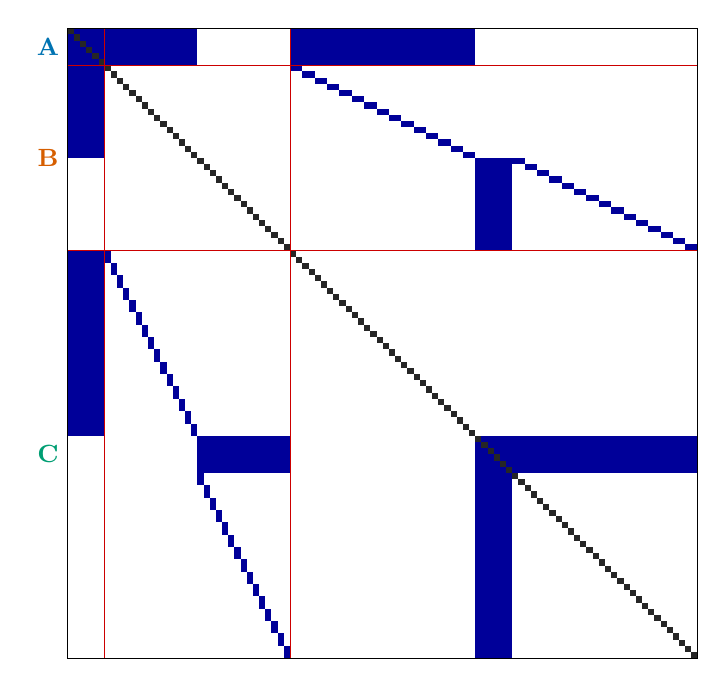
\begin{tikzpicture}[scale=1.0]
  \fill[black!85] (0.000,0.000) rectangle (0.078,-0.078);
  \fill[blue!60!black] (0.078,0.000) rectangle (0.157,-0.078);
  \fill[blue!60!black] (0.157,0.000) rectangle (0.235,-0.078);
  \fill[blue!60!black] (0.235,0.000) rectangle (0.314,-0.078);
  \fill[blue!60!black] (0.314,0.000) rectangle (0.392,-0.078);
  \fill[blue!60!black] (0.392,0.000) rectangle (0.471,-0.078);
  \fill[blue!60!black] (0.471,0.000) rectangle (0.549,-0.078);
  \fill[blue!60!black] (0.549,0.000) rectangle (0.627,-0.078);
  \fill[blue!60!black] (0.627,0.000) rectangle (0.706,-0.078);
  \fill[blue!60!black] (0.706,0.000) rectangle (0.784,-0.078);
  \fill[blue!60!black] (0.784,0.000) rectangle (0.863,-0.078);
  \fill[blue!60!black] (0.863,0.000) rectangle (0.941,-0.078);
  \fill[blue!60!black] (0.941,0.000) rectangle (1.020,-0.078);
  \fill[blue!60!black] (1.020,0.000) rectangle (1.098,-0.078);
  \fill[blue!60!black] (1.098,0.000) rectangle (1.176,-0.078);
  \fill[blue!60!black] (1.176,0.000) rectangle (1.255,-0.078);
  \fill[blue!60!black] (1.255,0.000) rectangle (1.333,-0.078);
  \fill[blue!60!black] (1.333,0.000) rectangle (1.412,-0.078);
  \fill[blue!60!black] (1.412,0.000) rectangle (1.490,-0.078);
  \fill[blue!60!black] (1.490,0.000) rectangle (1.569,-0.078);
  \fill[blue!60!black] (1.569,0.000) rectangle (1.647,-0.078);
  \fill[blue!60!black] (2.824,0.000) rectangle (2.902,-0.078);
  \fill[blue!60!black] (2.902,0.000) rectangle (2.980,-0.078);
  \fill[blue!60!black] (2.980,0.000) rectangle (3.059,-0.078);
  \fill[blue!60!black] (3.059,0.000) rectangle (3.137,-0.078);
  \fill[blue!60!black] (3.137,0.000) rectangle (3.216,-0.078);
  \fill[blue!60!black] (3.216,0.000) rectangle (3.294,-0.078);
  \fill[blue!60!black] (3.294,0.000) rectangle (3.373,-0.078);
  \fill[blue!60!black] (3.373,0.000) rectangle (3.451,-0.078);
  \fill[blue!60!black] (3.451,0.000) rectangle (3.529,-0.078);
  \fill[blue!60!black] (3.529,0.000) rectangle (3.608,-0.078);
  \fill[blue!60!black] (3.608,0.000) rectangle (3.686,-0.078);
  \fill[blue!60!black] (3.686,0.000) rectangle (3.765,-0.078);
  \fill[blue!60!black] (3.765,0.000) rectangle (3.843,-0.078);
  \fill[blue!60!black] (3.843,0.000) rectangle (3.922,-0.078);
  \fill[blue!60!black] (3.922,0.000) rectangle (4.000,-0.078);
  \fill[blue!60!black] (4.000,0.000) rectangle (4.078,-0.078);
  \fill[blue!60!black] (4.078,0.000) rectangle (4.157,-0.078);
  \fill[blue!60!black] (4.157,0.000) rectangle (4.235,-0.078);
  \fill[blue!60!black] (4.235,0.000) rectangle (4.314,-0.078);
  \fill[blue!60!black] (4.314,0.000) rectangle (4.392,-0.078);
  \fill[blue!60!black] (4.392,0.000) rectangle (4.471,-0.078);
  \fill[blue!60!black] (4.471,0.000) rectangle (4.549,-0.078);
  \fill[blue!60!black] (4.549,0.000) rectangle (4.627,-0.078);
  \fill[blue!60!black] (4.627,0.000) rectangle (4.706,-0.078);
  \fill[blue!60!black] (4.706,0.000) rectangle (4.784,-0.078);
  \fill[blue!60!black] (4.784,0.000) rectangle (4.863,-0.078);
  \fill[blue!60!black] (4.863,0.000) rectangle (4.941,-0.078);
  \fill[blue!60!black] (4.941,0.000) rectangle (5.020,-0.078);
  \fill[blue!60!black] (5.020,0.000) rectangle (5.098,-0.078);
  \fill[blue!60!black] (5.098,0.000) rectangle (5.176,-0.078);
  \fill[blue!60!black] (0.000,-0.078) rectangle (0.078,-0.157);
  \fill[black!85] (0.078,-0.078) rectangle (0.157,-0.157);
  \fill[blue!60!black] (0.157,-0.078) rectangle (0.235,-0.157);
  \fill[blue!60!black] (0.235,-0.078) rectangle (0.314,-0.157);
  \fill[blue!60!black] (0.314,-0.078) rectangle (0.392,-0.157);
  \fill[blue!60!black] (0.392,-0.078) rectangle (0.471,-0.157);
  \fill[blue!60!black] (0.471,-0.078) rectangle (0.549,-0.157);
  \fill[blue!60!black] (0.549,-0.078) rectangle (0.627,-0.157);
  \fill[blue!60!black] (0.627,-0.078) rectangle (0.706,-0.157);
  \fill[blue!60!black] (0.706,-0.078) rectangle (0.784,-0.157);
  \fill[blue!60!black] (0.784,-0.078) rectangle (0.863,-0.157);
  \fill[blue!60!black] (0.863,-0.078) rectangle (0.941,-0.157);
  \fill[blue!60!black] (0.941,-0.078) rectangle (1.020,-0.157);
  \fill[blue!60!black] (1.020,-0.078) rectangle (1.098,-0.157);
  \fill[blue!60!black] (1.098,-0.078) rectangle (1.176,-0.157);
  \fill[blue!60!black] (1.176,-0.078) rectangle (1.255,-0.157);
  \fill[blue!60!black] (1.255,-0.078) rectangle (1.333,-0.157);
  \fill[blue!60!black] (1.333,-0.078) rectangle (1.412,-0.157);
  \fill[blue!60!black] (1.412,-0.078) rectangle (1.490,-0.157);
  \fill[blue!60!black] (1.490,-0.078) rectangle (1.569,-0.157);
  \fill[blue!60!black] (1.569,-0.078) rectangle (1.647,-0.157);
  \fill[blue!60!black] (2.824,-0.078) rectangle (2.902,-0.157);
  \fill[blue!60!black] (2.902,-0.078) rectangle (2.980,-0.157);
  \fill[blue!60!black] (2.980,-0.078) rectangle (3.059,-0.157);
  \fill[blue!60!black] (3.059,-0.078) rectangle (3.137,-0.157);
  \fill[blue!60!black] (3.137,-0.078) rectangle (3.216,-0.157);
  \fill[blue!60!black] (3.216,-0.078) rectangle (3.294,-0.157);
  \fill[blue!60!black] (3.294,-0.078) rectangle (3.373,-0.157);
  \fill[blue!60!black] (3.373,-0.078) rectangle (3.451,-0.157);
  \fill[blue!60!black] (3.451,-0.078) rectangle (3.529,-0.157);
  \fill[blue!60!black] (3.529,-0.078) rectangle (3.608,-0.157);
  \fill[blue!60!black] (3.608,-0.078) rectangle (3.686,-0.157);
  \fill[blue!60!black] (3.686,-0.078) rectangle (3.765,-0.157);
  \fill[blue!60!black] (3.765,-0.078) rectangle (3.843,-0.157);
  \fill[blue!60!black] (3.843,-0.078) rectangle (3.922,-0.157);
  \fill[blue!60!black] (3.922,-0.078) rectangle (4.000,-0.157);
  \fill[blue!60!black] (4.000,-0.078) rectangle (4.078,-0.157);
  \fill[blue!60!black] (4.078,-0.078) rectangle (4.157,-0.157);
  \fill[blue!60!black] (4.157,-0.078) rectangle (4.235,-0.157);
  \fill[blue!60!black] (4.235,-0.078) rectangle (4.314,-0.157);
  \fill[blue!60!black] (4.314,-0.078) rectangle (4.392,-0.157);
  \fill[blue!60!black] (4.392,-0.078) rectangle (4.471,-0.157);
  \fill[blue!60!black] (4.471,-0.078) rectangle (4.549,-0.157);
  \fill[blue!60!black] (4.549,-0.078) rectangle (4.627,-0.157);
  \fill[blue!60!black] (4.627,-0.078) rectangle (4.706,-0.157);
  \fill[blue!60!black] (4.706,-0.078) rectangle (4.784,-0.157);
  \fill[blue!60!black] (4.784,-0.078) rectangle (4.863,-0.157);
  \fill[blue!60!black] (4.863,-0.078) rectangle (4.941,-0.157);
  \fill[blue!60!black] (4.941,-0.078) rectangle (5.020,-0.157);
  \fill[blue!60!black] (5.020,-0.078) rectangle (5.098,-0.157);
  \fill[blue!60!black] (5.098,-0.078) rectangle (5.176,-0.157);
  \fill[blue!60!black] (0.000,-0.157) rectangle (0.078,-0.235);
  \fill[blue!60!black] (0.078,-0.157) rectangle (0.157,-0.235);
  \fill[black!85] (0.157,-0.157) rectangle (0.235,-0.235);
  \fill[blue!60!black] (0.235,-0.157) rectangle (0.314,-0.235);
  \fill[blue!60!black] (0.314,-0.157) rectangle (0.392,-0.235);
  \fill[blue!60!black] (0.392,-0.157) rectangle (0.471,-0.235);
  \fill[blue!60!black] (0.471,-0.157) rectangle (0.549,-0.235);
  \fill[blue!60!black] (0.549,-0.157) rectangle (0.627,-0.235);
  \fill[blue!60!black] (0.627,-0.157) rectangle (0.706,-0.235);
  \fill[blue!60!black] (0.706,-0.157) rectangle (0.784,-0.235);
  \fill[blue!60!black] (0.784,-0.157) rectangle (0.863,-0.235);
  \fill[blue!60!black] (0.863,-0.157) rectangle (0.941,-0.235);
  \fill[blue!60!black] (0.941,-0.157) rectangle (1.020,-0.235);
  \fill[blue!60!black] (1.020,-0.157) rectangle (1.098,-0.235);
  \fill[blue!60!black] (1.098,-0.157) rectangle (1.176,-0.235);
  \fill[blue!60!black] (1.176,-0.157) rectangle (1.255,-0.235);
  \fill[blue!60!black] (1.255,-0.157) rectangle (1.333,-0.235);
  \fill[blue!60!black] (1.333,-0.157) rectangle (1.412,-0.235);
  \fill[blue!60!black] (1.412,-0.157) rectangle (1.490,-0.235);
  \fill[blue!60!black] (1.490,-0.157) rectangle (1.569,-0.235);
  \fill[blue!60!black] (1.569,-0.157) rectangle (1.647,-0.235);
  \fill[blue!60!black] (2.824,-0.157) rectangle (2.902,-0.235);
  \fill[blue!60!black] (2.902,-0.157) rectangle (2.980,-0.235);
  \fill[blue!60!black] (2.980,-0.157) rectangle (3.059,-0.235);
  \fill[blue!60!black] (3.059,-0.157) rectangle (3.137,-0.235);
  \fill[blue!60!black] (3.137,-0.157) rectangle (3.216,-0.235);
  \fill[blue!60!black] (3.216,-0.157) rectangle (3.294,-0.235);
  \fill[blue!60!black] (3.294,-0.157) rectangle (3.373,-0.235);
  \fill[blue!60!black] (3.373,-0.157) rectangle (3.451,-0.235);
  \fill[blue!60!black] (3.451,-0.157) rectangle (3.529,-0.235);
  \fill[blue!60!black] (3.529,-0.157) rectangle (3.608,-0.235);
  \fill[blue!60!black] (3.608,-0.157) rectangle (3.686,-0.235);
  \fill[blue!60!black] (3.686,-0.157) rectangle (3.765,-0.235);
  \fill[blue!60!black] (3.765,-0.157) rectangle (3.843,-0.235);
  \fill[blue!60!black] (3.843,-0.157) rectangle (3.922,-0.235);
  \fill[blue!60!black] (3.922,-0.157) rectangle (4.000,-0.235);
  \fill[blue!60!black] (4.000,-0.157) rectangle (4.078,-0.235);
  \fill[blue!60!black] (4.078,-0.157) rectangle (4.157,-0.235);
  \fill[blue!60!black] (4.157,-0.157) rectangle (4.235,-0.235);
  \fill[blue!60!black] (4.235,-0.157) rectangle (4.314,-0.235);
  \fill[blue!60!black] (4.314,-0.157) rectangle (4.392,-0.235);
  \fill[blue!60!black] (4.392,-0.157) rectangle (4.471,-0.235);
  \fill[blue!60!black] (4.471,-0.157) rectangle (4.549,-0.235);
  \fill[blue!60!black] (4.549,-0.157) rectangle (4.627,-0.235);
  \fill[blue!60!black] (4.627,-0.157) rectangle (4.706,-0.235);
  \fill[blue!60!black] (4.706,-0.157) rectangle (4.784,-0.235);
  \fill[blue!60!black] (4.784,-0.157) rectangle (4.863,-0.235);
  \fill[blue!60!black] (4.863,-0.157) rectangle (4.941,-0.235);
  \fill[blue!60!black] (4.941,-0.157) rectangle (5.020,-0.235);
  \fill[blue!60!black] (5.020,-0.157) rectangle (5.098,-0.235);
  \fill[blue!60!black] (5.098,-0.157) rectangle (5.176,-0.235);
  \fill[blue!60!black] (0.000,-0.235) rectangle (0.078,-0.314);
  \fill[blue!60!black] (0.078,-0.235) rectangle (0.157,-0.314);
  \fill[blue!60!black] (0.157,-0.235) rectangle (0.235,-0.314);
  \fill[black!85] (0.235,-0.235) rectangle (0.314,-0.314);
  \fill[blue!60!black] (0.314,-0.235) rectangle (0.392,-0.314);
  \fill[blue!60!black] (0.392,-0.235) rectangle (0.471,-0.314);
  \fill[blue!60!black] (0.471,-0.235) rectangle (0.549,-0.314);
  \fill[blue!60!black] (0.549,-0.235) rectangle (0.627,-0.314);
  \fill[blue!60!black] (0.627,-0.235) rectangle (0.706,-0.314);
  \fill[blue!60!black] (0.706,-0.235) rectangle (0.784,-0.314);
  \fill[blue!60!black] (0.784,-0.235) rectangle (0.863,-0.314);
  \fill[blue!60!black] (0.863,-0.235) rectangle (0.941,-0.314);
  \fill[blue!60!black] (0.941,-0.235) rectangle (1.020,-0.314);
  \fill[blue!60!black] (1.020,-0.235) rectangle (1.098,-0.314);
  \fill[blue!60!black] (1.098,-0.235) rectangle (1.176,-0.314);
  \fill[blue!60!black] (1.176,-0.235) rectangle (1.255,-0.314);
  \fill[blue!60!black] (1.255,-0.235) rectangle (1.333,-0.314);
  \fill[blue!60!black] (1.333,-0.235) rectangle (1.412,-0.314);
  \fill[blue!60!black] (1.412,-0.235) rectangle (1.490,-0.314);
  \fill[blue!60!black] (1.490,-0.235) rectangle (1.569,-0.314);
  \fill[blue!60!black] (1.569,-0.235) rectangle (1.647,-0.314);
  \fill[blue!60!black] (2.824,-0.235) rectangle (2.902,-0.314);
  \fill[blue!60!black] (2.902,-0.235) rectangle (2.980,-0.314);
  \fill[blue!60!black] (2.980,-0.235) rectangle (3.059,-0.314);
  \fill[blue!60!black] (3.059,-0.235) rectangle (3.137,-0.314);
  \fill[blue!60!black] (3.137,-0.235) rectangle (3.216,-0.314);
  \fill[blue!60!black] (3.216,-0.235) rectangle (3.294,-0.314);
  \fill[blue!60!black] (3.294,-0.235) rectangle (3.373,-0.314);
  \fill[blue!60!black] (3.373,-0.235) rectangle (3.451,-0.314);
  \fill[blue!60!black] (3.451,-0.235) rectangle (3.529,-0.314);
  \fill[blue!60!black] (3.529,-0.235) rectangle (3.608,-0.314);
  \fill[blue!60!black] (3.608,-0.235) rectangle (3.686,-0.314);
  \fill[blue!60!black] (3.686,-0.235) rectangle (3.765,-0.314);
  \fill[blue!60!black] (3.765,-0.235) rectangle (3.843,-0.314);
  \fill[blue!60!black] (3.843,-0.235) rectangle (3.922,-0.314);
  \fill[blue!60!black] (3.922,-0.235) rectangle (4.000,-0.314);
  \fill[blue!60!black] (4.000,-0.235) rectangle (4.078,-0.314);
  \fill[blue!60!black] (4.078,-0.235) rectangle (4.157,-0.314);
  \fill[blue!60!black] (4.157,-0.235) rectangle (4.235,-0.314);
  \fill[blue!60!black] (4.235,-0.235) rectangle (4.314,-0.314);
  \fill[blue!60!black] (4.314,-0.235) rectangle (4.392,-0.314);
  \fill[blue!60!black] (4.392,-0.235) rectangle (4.471,-0.314);
  \fill[blue!60!black] (4.471,-0.235) rectangle (4.549,-0.314);
  \fill[blue!60!black] (4.549,-0.235) rectangle (4.627,-0.314);
  \fill[blue!60!black] (4.627,-0.235) rectangle (4.706,-0.314);
  \fill[blue!60!black] (4.706,-0.235) rectangle (4.784,-0.314);
  \fill[blue!60!black] (4.784,-0.235) rectangle (4.863,-0.314);
  \fill[blue!60!black] (4.863,-0.235) rectangle (4.941,-0.314);
  \fill[blue!60!black] (4.941,-0.235) rectangle (5.020,-0.314);
  \fill[blue!60!black] (5.020,-0.235) rectangle (5.098,-0.314);
  \fill[blue!60!black] (5.098,-0.235) rectangle (5.176,-0.314);
  \fill[blue!60!black] (0.000,-0.314) rectangle (0.078,-0.392);
  \fill[blue!60!black] (0.078,-0.314) rectangle (0.157,-0.392);
  \fill[blue!60!black] (0.157,-0.314) rectangle (0.235,-0.392);
  \fill[blue!60!black] (0.235,-0.314) rectangle (0.314,-0.392);
  \fill[black!85] (0.314,-0.314) rectangle (0.392,-0.392);
  \fill[blue!60!black] (0.392,-0.314) rectangle (0.471,-0.392);
  \fill[blue!60!black] (0.471,-0.314) rectangle (0.549,-0.392);
  \fill[blue!60!black] (0.549,-0.314) rectangle (0.627,-0.392);
  \fill[blue!60!black] (0.627,-0.314) rectangle (0.706,-0.392);
  \fill[blue!60!black] (0.706,-0.314) rectangle (0.784,-0.392);
  \fill[blue!60!black] (0.784,-0.314) rectangle (0.863,-0.392);
  \fill[blue!60!black] (0.863,-0.314) rectangle (0.941,-0.392);
  \fill[blue!60!black] (0.941,-0.314) rectangle (1.020,-0.392);
  \fill[blue!60!black] (1.020,-0.314) rectangle (1.098,-0.392);
  \fill[blue!60!black] (1.098,-0.314) rectangle (1.176,-0.392);
  \fill[blue!60!black] (1.176,-0.314) rectangle (1.255,-0.392);
  \fill[blue!60!black] (1.255,-0.314) rectangle (1.333,-0.392);
  \fill[blue!60!black] (1.333,-0.314) rectangle (1.412,-0.392);
  \fill[blue!60!black] (1.412,-0.314) rectangle (1.490,-0.392);
  \fill[blue!60!black] (1.490,-0.314) rectangle (1.569,-0.392);
  \fill[blue!60!black] (1.569,-0.314) rectangle (1.647,-0.392);
  \fill[blue!60!black] (2.824,-0.314) rectangle (2.902,-0.392);
  \fill[blue!60!black] (2.902,-0.314) rectangle (2.980,-0.392);
  \fill[blue!60!black] (2.980,-0.314) rectangle (3.059,-0.392);
  \fill[blue!60!black] (3.059,-0.314) rectangle (3.137,-0.392);
  \fill[blue!60!black] (3.137,-0.314) rectangle (3.216,-0.392);
  \fill[blue!60!black] (3.216,-0.314) rectangle (3.294,-0.392);
  \fill[blue!60!black] (3.294,-0.314) rectangle (3.373,-0.392);
  \fill[blue!60!black] (3.373,-0.314) rectangle (3.451,-0.392);
  \fill[blue!60!black] (3.451,-0.314) rectangle (3.529,-0.392);
  \fill[blue!60!black] (3.529,-0.314) rectangle (3.608,-0.392);
  \fill[blue!60!black] (3.608,-0.314) rectangle (3.686,-0.392);
  \fill[blue!60!black] (3.686,-0.314) rectangle (3.765,-0.392);
  \fill[blue!60!black] (3.765,-0.314) rectangle (3.843,-0.392);
  \fill[blue!60!black] (3.843,-0.314) rectangle (3.922,-0.392);
  \fill[blue!60!black] (3.922,-0.314) rectangle (4.000,-0.392);
  \fill[blue!60!black] (4.000,-0.314) rectangle (4.078,-0.392);
  \fill[blue!60!black] (4.078,-0.314) rectangle (4.157,-0.392);
  \fill[blue!60!black] (4.157,-0.314) rectangle (4.235,-0.392);
  \fill[blue!60!black] (4.235,-0.314) rectangle (4.314,-0.392);
  \fill[blue!60!black] (4.314,-0.314) rectangle (4.392,-0.392);
  \fill[blue!60!black] (4.392,-0.314) rectangle (4.471,-0.392);
  \fill[blue!60!black] (4.471,-0.314) rectangle (4.549,-0.392);
  \fill[blue!60!black] (4.549,-0.314) rectangle (4.627,-0.392);
  \fill[blue!60!black] (4.627,-0.314) rectangle (4.706,-0.392);
  \fill[blue!60!black] (4.706,-0.314) rectangle (4.784,-0.392);
  \fill[blue!60!black] (4.784,-0.314) rectangle (4.863,-0.392);
  \fill[blue!60!black] (4.863,-0.314) rectangle (4.941,-0.392);
  \fill[blue!60!black] (4.941,-0.314) rectangle (5.020,-0.392);
  \fill[blue!60!black] (5.020,-0.314) rectangle (5.098,-0.392);
  \fill[blue!60!black] (5.098,-0.314) rectangle (5.176,-0.392);
  \fill[blue!60!black] (0.000,-0.392) rectangle (0.078,-0.471);
  \fill[blue!60!black] (0.078,-0.392) rectangle (0.157,-0.471);
  \fill[blue!60!black] (0.157,-0.392) rectangle (0.235,-0.471);
  \fill[blue!60!black] (0.235,-0.392) rectangle (0.314,-0.471);
  \fill[blue!60!black] (0.314,-0.392) rectangle (0.392,-0.471);
  \fill[black!85] (0.392,-0.392) rectangle (0.471,-0.471);
  \fill[blue!60!black] (0.471,-0.392) rectangle (0.549,-0.471);
  \fill[blue!60!black] (0.549,-0.392) rectangle (0.627,-0.471);
  \fill[blue!60!black] (0.627,-0.392) rectangle (0.706,-0.471);
  \fill[blue!60!black] (0.706,-0.392) rectangle (0.784,-0.471);
  \fill[blue!60!black] (0.784,-0.392) rectangle (0.863,-0.471);
  \fill[blue!60!black] (0.863,-0.392) rectangle (0.941,-0.471);
  \fill[blue!60!black] (0.941,-0.392) rectangle (1.020,-0.471);
  \fill[blue!60!black] (1.020,-0.392) rectangle (1.098,-0.471);
  \fill[blue!60!black] (1.098,-0.392) rectangle (1.176,-0.471);
  \fill[blue!60!black] (1.176,-0.392) rectangle (1.255,-0.471);
  \fill[blue!60!black] (1.255,-0.392) rectangle (1.333,-0.471);
  \fill[blue!60!black] (1.333,-0.392) rectangle (1.412,-0.471);
  \fill[blue!60!black] (1.412,-0.392) rectangle (1.490,-0.471);
  \fill[blue!60!black] (1.490,-0.392) rectangle (1.569,-0.471);
  \fill[blue!60!black] (1.569,-0.392) rectangle (1.647,-0.471);
  \fill[blue!60!black] (2.824,-0.392) rectangle (2.902,-0.471);
  \fill[blue!60!black] (2.902,-0.392) rectangle (2.980,-0.471);
  \fill[blue!60!black] (2.980,-0.392) rectangle (3.059,-0.471);
  \fill[blue!60!black] (3.059,-0.392) rectangle (3.137,-0.471);
  \fill[blue!60!black] (3.137,-0.392) rectangle (3.216,-0.471);
  \fill[blue!60!black] (3.216,-0.392) rectangle (3.294,-0.471);
  \fill[blue!60!black] (3.294,-0.392) rectangle (3.373,-0.471);
  \fill[blue!60!black] (3.373,-0.392) rectangle (3.451,-0.471);
  \fill[blue!60!black] (3.451,-0.392) rectangle (3.529,-0.471);
  \fill[blue!60!black] (3.529,-0.392) rectangle (3.608,-0.471);
  \fill[blue!60!black] (3.608,-0.392) rectangle (3.686,-0.471);
  \fill[blue!60!black] (3.686,-0.392) rectangle (3.765,-0.471);
  \fill[blue!60!black] (3.765,-0.392) rectangle (3.843,-0.471);
  \fill[blue!60!black] (3.843,-0.392) rectangle (3.922,-0.471);
  \fill[blue!60!black] (3.922,-0.392) rectangle (4.000,-0.471);
  \fill[blue!60!black] (4.000,-0.392) rectangle (4.078,-0.471);
  \fill[blue!60!black] (4.078,-0.392) rectangle (4.157,-0.471);
  \fill[blue!60!black] (4.157,-0.392) rectangle (4.235,-0.471);
  \fill[blue!60!black] (4.235,-0.392) rectangle (4.314,-0.471);
  \fill[blue!60!black] (4.314,-0.392) rectangle (4.392,-0.471);
  \fill[blue!60!black] (4.392,-0.392) rectangle (4.471,-0.471);
  \fill[blue!60!black] (4.471,-0.392) rectangle (4.549,-0.471);
  \fill[blue!60!black] (4.549,-0.392) rectangle (4.627,-0.471);
  \fill[blue!60!black] (4.627,-0.392) rectangle (4.706,-0.471);
  \fill[blue!60!black] (4.706,-0.392) rectangle (4.784,-0.471);
  \fill[blue!60!black] (4.784,-0.392) rectangle (4.863,-0.471);
  \fill[blue!60!black] (4.863,-0.392) rectangle (4.941,-0.471);
  \fill[blue!60!black] (4.941,-0.392) rectangle (5.020,-0.471);
  \fill[blue!60!black] (5.020,-0.392) rectangle (5.098,-0.471);
  \fill[blue!60!black] (5.098,-0.392) rectangle (5.176,-0.471);
  \fill[blue!60!black] (0.000,-0.471) rectangle (0.078,-0.549);
  \fill[blue!60!black] (0.078,-0.471) rectangle (0.157,-0.549);
  \fill[blue!60!black] (0.157,-0.471) rectangle (0.235,-0.549);
  \fill[blue!60!black] (0.235,-0.471) rectangle (0.314,-0.549);
  \fill[blue!60!black] (0.314,-0.471) rectangle (0.392,-0.549);
  \fill[blue!60!black] (0.392,-0.471) rectangle (0.471,-0.549);
  \fill[black!85] (0.471,-0.471) rectangle (0.549,-0.549);
  \fill[blue!60!black] (2.824,-0.471) rectangle (2.902,-0.549);
  \fill[blue!60!black] (2.902,-0.471) rectangle (2.980,-0.549);
  \fill[blue!60!black] (0.000,-0.549) rectangle (0.078,-0.627);
  \fill[blue!60!black] (0.078,-0.549) rectangle (0.157,-0.627);
  \fill[blue!60!black] (0.157,-0.549) rectangle (0.235,-0.627);
  \fill[blue!60!black] (0.235,-0.549) rectangle (0.314,-0.627);
  \fill[blue!60!black] (0.314,-0.549) rectangle (0.392,-0.627);
  \fill[blue!60!black] (0.392,-0.549) rectangle (0.471,-0.627);
  \fill[black!85] (0.549,-0.549) rectangle (0.627,-0.627);
  \fill[blue!60!black] (2.980,-0.549) rectangle (3.059,-0.627);
  \fill[blue!60!black] (3.059,-0.549) rectangle (3.137,-0.627);
  \fill[blue!60!black] (0.000,-0.627) rectangle (0.078,-0.706);
  \fill[blue!60!black] (0.078,-0.627) rectangle (0.157,-0.706);
  \fill[blue!60!black] (0.157,-0.627) rectangle (0.235,-0.706);
  \fill[blue!60!black] (0.235,-0.627) rectangle (0.314,-0.706);
  \fill[blue!60!black] (0.314,-0.627) rectangle (0.392,-0.706);
  \fill[blue!60!black] (0.392,-0.627) rectangle (0.471,-0.706);
  \fill[black!85] (0.627,-0.627) rectangle (0.706,-0.706);
  \fill[blue!60!black] (3.137,-0.627) rectangle (3.216,-0.706);
  \fill[blue!60!black] (3.216,-0.627) rectangle (3.294,-0.706);
  \fill[blue!60!black] (0.000,-0.706) rectangle (0.078,-0.784);
  \fill[blue!60!black] (0.078,-0.706) rectangle (0.157,-0.784);
  \fill[blue!60!black] (0.157,-0.706) rectangle (0.235,-0.784);
  \fill[blue!60!black] (0.235,-0.706) rectangle (0.314,-0.784);
  \fill[blue!60!black] (0.314,-0.706) rectangle (0.392,-0.784);
  \fill[blue!60!black] (0.392,-0.706) rectangle (0.471,-0.784);
  \fill[black!85] (0.706,-0.706) rectangle (0.784,-0.784);
  \fill[blue!60!black] (3.294,-0.706) rectangle (3.373,-0.784);
  \fill[blue!60!black] (3.373,-0.706) rectangle (3.451,-0.784);
  \fill[blue!60!black] (0.000,-0.784) rectangle (0.078,-0.863);
  \fill[blue!60!black] (0.078,-0.784) rectangle (0.157,-0.863);
  \fill[blue!60!black] (0.157,-0.784) rectangle (0.235,-0.863);
  \fill[blue!60!black] (0.235,-0.784) rectangle (0.314,-0.863);
  \fill[blue!60!black] (0.314,-0.784) rectangle (0.392,-0.863);
  \fill[blue!60!black] (0.392,-0.784) rectangle (0.471,-0.863);
  \fill[black!85] (0.784,-0.784) rectangle (0.863,-0.863);
  \fill[blue!60!black] (3.451,-0.784) rectangle (3.529,-0.863);
  \fill[blue!60!black] (3.529,-0.784) rectangle (3.608,-0.863);
  \fill[blue!60!black] (0.000,-0.863) rectangle (0.078,-0.941);
  \fill[blue!60!black] (0.078,-0.863) rectangle (0.157,-0.941);
  \fill[blue!60!black] (0.157,-0.863) rectangle (0.235,-0.941);
  \fill[blue!60!black] (0.235,-0.863) rectangle (0.314,-0.941);
  \fill[blue!60!black] (0.314,-0.863) rectangle (0.392,-0.941);
  \fill[blue!60!black] (0.392,-0.863) rectangle (0.471,-0.941);
  \fill[black!85] (0.863,-0.863) rectangle (0.941,-0.941);
  \fill[blue!60!black] (3.608,-0.863) rectangle (3.686,-0.941);
  \fill[blue!60!black] (3.686,-0.863) rectangle (3.765,-0.941);
  \fill[blue!60!black] (0.000,-0.941) rectangle (0.078,-1.020);
  \fill[blue!60!black] (0.078,-0.941) rectangle (0.157,-1.020);
  \fill[blue!60!black] (0.157,-0.941) rectangle (0.235,-1.020);
  \fill[blue!60!black] (0.235,-0.941) rectangle (0.314,-1.020);
  \fill[blue!60!black] (0.314,-0.941) rectangle (0.392,-1.020);
  \fill[blue!60!black] (0.392,-0.941) rectangle (0.471,-1.020);
  \fill[black!85] (0.941,-0.941) rectangle (1.020,-1.020);
  \fill[blue!60!black] (3.765,-0.941) rectangle (3.843,-1.020);
  \fill[blue!60!black] (3.843,-0.941) rectangle (3.922,-1.020);
  \fill[blue!60!black] (0.000,-1.020) rectangle (0.078,-1.098);
  \fill[blue!60!black] (0.078,-1.020) rectangle (0.157,-1.098);
  \fill[blue!60!black] (0.157,-1.020) rectangle (0.235,-1.098);
  \fill[blue!60!black] (0.235,-1.020) rectangle (0.314,-1.098);
  \fill[blue!60!black] (0.314,-1.020) rectangle (0.392,-1.098);
  \fill[blue!60!black] (0.392,-1.020) rectangle (0.471,-1.098);
  \fill[black!85] (1.020,-1.020) rectangle (1.098,-1.098);
  \fill[blue!60!black] (3.922,-1.020) rectangle (4.000,-1.098);
  \fill[blue!60!black] (4.000,-1.020) rectangle (4.078,-1.098);
  \fill[blue!60!black] (0.000,-1.098) rectangle (0.078,-1.176);
  \fill[blue!60!black] (0.078,-1.098) rectangle (0.157,-1.176);
  \fill[blue!60!black] (0.157,-1.098) rectangle (0.235,-1.176);
  \fill[blue!60!black] (0.235,-1.098) rectangle (0.314,-1.176);
  \fill[blue!60!black] (0.314,-1.098) rectangle (0.392,-1.176);
  \fill[blue!60!black] (0.392,-1.098) rectangle (0.471,-1.176);
  \fill[black!85] (1.098,-1.098) rectangle (1.176,-1.176);
  \fill[blue!60!black] (4.078,-1.098) rectangle (4.157,-1.176);
  \fill[blue!60!black] (4.157,-1.098) rectangle (4.235,-1.176);
  \fill[blue!60!black] (0.000,-1.176) rectangle (0.078,-1.255);
  \fill[blue!60!black] (0.078,-1.176) rectangle (0.157,-1.255);
  \fill[blue!60!black] (0.157,-1.176) rectangle (0.235,-1.255);
  \fill[blue!60!black] (0.235,-1.176) rectangle (0.314,-1.255);
  \fill[blue!60!black] (0.314,-1.176) rectangle (0.392,-1.255);
  \fill[blue!60!black] (0.392,-1.176) rectangle (0.471,-1.255);
  \fill[black!85] (1.176,-1.176) rectangle (1.255,-1.255);
  \fill[blue!60!black] (4.235,-1.176) rectangle (4.314,-1.255);
  \fill[blue!60!black] (4.314,-1.176) rectangle (4.392,-1.255);
  \fill[blue!60!black] (0.000,-1.255) rectangle (0.078,-1.333);
  \fill[blue!60!black] (0.078,-1.255) rectangle (0.157,-1.333);
  \fill[blue!60!black] (0.157,-1.255) rectangle (0.235,-1.333);
  \fill[blue!60!black] (0.235,-1.255) rectangle (0.314,-1.333);
  \fill[blue!60!black] (0.314,-1.255) rectangle (0.392,-1.333);
  \fill[blue!60!black] (0.392,-1.255) rectangle (0.471,-1.333);
  \fill[black!85] (1.255,-1.255) rectangle (1.333,-1.333);
  \fill[blue!60!black] (4.392,-1.255) rectangle (4.471,-1.333);
  \fill[blue!60!black] (4.471,-1.255) rectangle (4.549,-1.333);
  \fill[blue!60!black] (0.000,-1.333) rectangle (0.078,-1.412);
  \fill[blue!60!black] (0.078,-1.333) rectangle (0.157,-1.412);
  \fill[blue!60!black] (0.157,-1.333) rectangle (0.235,-1.412);
  \fill[blue!60!black] (0.235,-1.333) rectangle (0.314,-1.412);
  \fill[blue!60!black] (0.314,-1.333) rectangle (0.392,-1.412);
  \fill[blue!60!black] (0.392,-1.333) rectangle (0.471,-1.412);
  \fill[black!85] (1.333,-1.333) rectangle (1.412,-1.412);
  \fill[blue!60!black] (4.549,-1.333) rectangle (4.627,-1.412);
  \fill[blue!60!black] (4.627,-1.333) rectangle (4.706,-1.412);
  \fill[blue!60!black] (0.000,-1.412) rectangle (0.078,-1.490);
  \fill[blue!60!black] (0.078,-1.412) rectangle (0.157,-1.490);
  \fill[blue!60!black] (0.157,-1.412) rectangle (0.235,-1.490);
  \fill[blue!60!black] (0.235,-1.412) rectangle (0.314,-1.490);
  \fill[blue!60!black] (0.314,-1.412) rectangle (0.392,-1.490);
  \fill[blue!60!black] (0.392,-1.412) rectangle (0.471,-1.490);
  \fill[black!85] (1.412,-1.412) rectangle (1.490,-1.490);
  \fill[blue!60!black] (4.706,-1.412) rectangle (4.784,-1.490);
  \fill[blue!60!black] (4.784,-1.412) rectangle (4.863,-1.490);
  \fill[blue!60!black] (0.000,-1.490) rectangle (0.078,-1.569);
  \fill[blue!60!black] (0.078,-1.490) rectangle (0.157,-1.569);
  \fill[blue!60!black] (0.157,-1.490) rectangle (0.235,-1.569);
  \fill[blue!60!black] (0.235,-1.490) rectangle (0.314,-1.569);
  \fill[blue!60!black] (0.314,-1.490) rectangle (0.392,-1.569);
  \fill[blue!60!black] (0.392,-1.490) rectangle (0.471,-1.569);
  \fill[black!85] (1.490,-1.490) rectangle (1.569,-1.569);
  \fill[blue!60!black] (4.863,-1.490) rectangle (4.941,-1.569);
  \fill[blue!60!black] (4.941,-1.490) rectangle (5.020,-1.569);
  \fill[blue!60!black] (0.000,-1.569) rectangle (0.078,-1.647);
  \fill[blue!60!black] (0.078,-1.569) rectangle (0.157,-1.647);
  \fill[blue!60!black] (0.157,-1.569) rectangle (0.235,-1.647);
  \fill[blue!60!black] (0.235,-1.569) rectangle (0.314,-1.647);
  \fill[blue!60!black] (0.314,-1.569) rectangle (0.392,-1.647);
  \fill[blue!60!black] (0.392,-1.569) rectangle (0.471,-1.647);
  \fill[black!85] (1.569,-1.569) rectangle (1.647,-1.647);
  \fill[blue!60!black] (5.020,-1.569) rectangle (5.098,-1.647);
  \fill[blue!60!black] (5.098,-1.569) rectangle (5.176,-1.647);
  \fill[black!85] (1.647,-1.647) rectangle (1.725,-1.725);
  \fill[blue!60!black] (5.176,-1.647) rectangle (5.255,-1.725);
  \fill[blue!60!black] (5.255,-1.647) rectangle (5.333,-1.725);
  \fill[blue!60!black] (5.333,-1.647) rectangle (5.412,-1.725);
  \fill[blue!60!black] (5.412,-1.647) rectangle (5.490,-1.725);
  \fill[blue!60!black] (5.490,-1.647) rectangle (5.569,-1.725);
  \fill[blue!60!black] (5.569,-1.647) rectangle (5.647,-1.725);
  \fill[blue!60!black] (5.647,-1.647) rectangle (5.725,-1.725);
  \fill[blue!60!black] (5.725,-1.647) rectangle (5.804,-1.725);
  \fill[black!85] (1.725,-1.725) rectangle (1.804,-1.804);
  \fill[blue!60!black] (5.176,-1.725) rectangle (5.255,-1.804);
  \fill[blue!60!black] (5.255,-1.725) rectangle (5.333,-1.804);
  \fill[blue!60!black] (5.333,-1.725) rectangle (5.412,-1.804);
  \fill[blue!60!black] (5.412,-1.725) rectangle (5.490,-1.804);
  \fill[blue!60!black] (5.490,-1.725) rectangle (5.569,-1.804);
  \fill[blue!60!black] (5.569,-1.725) rectangle (5.647,-1.804);
  \fill[blue!60!black] (5.804,-1.725) rectangle (5.882,-1.804);
  \fill[blue!60!black] (5.882,-1.725) rectangle (5.961,-1.804);
  \fill[black!85] (1.804,-1.804) rectangle (1.882,-1.882);
  \fill[blue!60!black] (5.176,-1.804) rectangle (5.255,-1.882);
  \fill[blue!60!black] (5.255,-1.804) rectangle (5.333,-1.882);
  \fill[blue!60!black] (5.333,-1.804) rectangle (5.412,-1.882);
  \fill[blue!60!black] (5.412,-1.804) rectangle (5.490,-1.882);
  \fill[blue!60!black] (5.490,-1.804) rectangle (5.569,-1.882);
  \fill[blue!60!black] (5.569,-1.804) rectangle (5.647,-1.882);
  \fill[blue!60!black] (5.961,-1.804) rectangle (6.039,-1.882);
  \fill[blue!60!black] (6.039,-1.804) rectangle (6.118,-1.882);
  \fill[black!85] (1.882,-1.882) rectangle (1.961,-1.961);
  \fill[blue!60!black] (5.176,-1.882) rectangle (5.255,-1.961);
  \fill[blue!60!black] (5.255,-1.882) rectangle (5.333,-1.961);
  \fill[blue!60!black] (5.333,-1.882) rectangle (5.412,-1.961);
  \fill[blue!60!black] (5.412,-1.882) rectangle (5.490,-1.961);
  \fill[blue!60!black] (5.490,-1.882) rectangle (5.569,-1.961);
  \fill[blue!60!black] (5.569,-1.882) rectangle (5.647,-1.961);
  \fill[blue!60!black] (6.118,-1.882) rectangle (6.196,-1.961);
  \fill[blue!60!black] (6.196,-1.882) rectangle (6.275,-1.961);
  \fill[black!85] (1.961,-1.961) rectangle (2.039,-2.039);
  \fill[blue!60!black] (5.176,-1.961) rectangle (5.255,-2.039);
  \fill[blue!60!black] (5.255,-1.961) rectangle (5.333,-2.039);
  \fill[blue!60!black] (5.333,-1.961) rectangle (5.412,-2.039);
  \fill[blue!60!black] (5.412,-1.961) rectangle (5.490,-2.039);
  \fill[blue!60!black] (5.490,-1.961) rectangle (5.569,-2.039);
  \fill[blue!60!black] (5.569,-1.961) rectangle (5.647,-2.039);
  \fill[blue!60!black] (6.275,-1.961) rectangle (6.353,-2.039);
  \fill[blue!60!black] (6.353,-1.961) rectangle (6.431,-2.039);
  \fill[black!85] (2.039,-2.039) rectangle (2.118,-2.118);
  \fill[blue!60!black] (5.176,-2.039) rectangle (5.255,-2.118);
  \fill[blue!60!black] (5.255,-2.039) rectangle (5.333,-2.118);
  \fill[blue!60!black] (5.333,-2.039) rectangle (5.412,-2.118);
  \fill[blue!60!black] (5.412,-2.039) rectangle (5.490,-2.118);
  \fill[blue!60!black] (5.490,-2.039) rectangle (5.569,-2.118);
  \fill[blue!60!black] (5.569,-2.039) rectangle (5.647,-2.118);
  \fill[blue!60!black] (6.431,-2.039) rectangle (6.510,-2.118);
  \fill[blue!60!black] (6.510,-2.039) rectangle (6.588,-2.118);
  \fill[black!85] (2.118,-2.118) rectangle (2.196,-2.196);
  \fill[blue!60!black] (5.176,-2.118) rectangle (5.255,-2.196);
  \fill[blue!60!black] (5.255,-2.118) rectangle (5.333,-2.196);
  \fill[blue!60!black] (5.333,-2.118) rectangle (5.412,-2.196);
  \fill[blue!60!black] (5.412,-2.118) rectangle (5.490,-2.196);
  \fill[blue!60!black] (5.490,-2.118) rectangle (5.569,-2.196);
  \fill[blue!60!black] (5.569,-2.118) rectangle (5.647,-2.196);
  \fill[blue!60!black] (6.588,-2.118) rectangle (6.667,-2.196);
  \fill[blue!60!black] (6.667,-2.118) rectangle (6.745,-2.196);
  \fill[black!85] (2.196,-2.196) rectangle (2.275,-2.275);
  \fill[blue!60!black] (5.176,-2.196) rectangle (5.255,-2.275);
  \fill[blue!60!black] (5.255,-2.196) rectangle (5.333,-2.275);
  \fill[blue!60!black] (5.333,-2.196) rectangle (5.412,-2.275);
  \fill[blue!60!black] (5.412,-2.196) rectangle (5.490,-2.275);
  \fill[blue!60!black] (5.490,-2.196) rectangle (5.569,-2.275);
  \fill[blue!60!black] (5.569,-2.196) rectangle (5.647,-2.275);
  \fill[blue!60!black] (6.745,-2.196) rectangle (6.824,-2.275);
  \fill[blue!60!black] (6.824,-2.196) rectangle (6.902,-2.275);
  \fill[black!85] (2.275,-2.275) rectangle (2.353,-2.353);
  \fill[blue!60!black] (5.176,-2.275) rectangle (5.255,-2.353);
  \fill[blue!60!black] (5.255,-2.275) rectangle (5.333,-2.353);
  \fill[blue!60!black] (5.333,-2.275) rectangle (5.412,-2.353);
  \fill[blue!60!black] (5.412,-2.275) rectangle (5.490,-2.353);
  \fill[blue!60!black] (5.490,-2.275) rectangle (5.569,-2.353);
  \fill[blue!60!black] (5.569,-2.275) rectangle (5.647,-2.353);
  \fill[blue!60!black] (6.902,-2.275) rectangle (6.980,-2.353);
  \fill[blue!60!black] (6.980,-2.275) rectangle (7.059,-2.353);
  \fill[black!85] (2.353,-2.353) rectangle (2.431,-2.431);
  \fill[blue!60!black] (5.176,-2.353) rectangle (5.255,-2.431);
  \fill[blue!60!black] (5.255,-2.353) rectangle (5.333,-2.431);
  \fill[blue!60!black] (5.333,-2.353) rectangle (5.412,-2.431);
  \fill[blue!60!black] (5.412,-2.353) rectangle (5.490,-2.431);
  \fill[blue!60!black] (5.490,-2.353) rectangle (5.569,-2.431);
  \fill[blue!60!black] (5.569,-2.353) rectangle (5.647,-2.431);
  \fill[blue!60!black] (7.059,-2.353) rectangle (7.137,-2.431);
  \fill[blue!60!black] (7.137,-2.353) rectangle (7.216,-2.431);
  \fill[black!85] (2.431,-2.431) rectangle (2.510,-2.510);
  \fill[blue!60!black] (5.176,-2.431) rectangle (5.255,-2.510);
  \fill[blue!60!black] (5.255,-2.431) rectangle (5.333,-2.510);
  \fill[blue!60!black] (5.333,-2.431) rectangle (5.412,-2.510);
  \fill[blue!60!black] (5.412,-2.431) rectangle (5.490,-2.510);
  \fill[blue!60!black] (5.490,-2.431) rectangle (5.569,-2.510);
  \fill[blue!60!black] (5.569,-2.431) rectangle (5.647,-2.510);
  \fill[blue!60!black] (7.216,-2.431) rectangle (7.294,-2.510);
  \fill[blue!60!black] (7.294,-2.431) rectangle (7.373,-2.510);
  \fill[black!85] (2.510,-2.510) rectangle (2.588,-2.588);
  \fill[blue!60!black] (5.176,-2.510) rectangle (5.255,-2.588);
  \fill[blue!60!black] (5.255,-2.510) rectangle (5.333,-2.588);
  \fill[blue!60!black] (5.333,-2.510) rectangle (5.412,-2.588);
  \fill[blue!60!black] (5.412,-2.510) rectangle (5.490,-2.588);
  \fill[blue!60!black] (5.490,-2.510) rectangle (5.569,-2.588);
  \fill[blue!60!black] (5.569,-2.510) rectangle (5.647,-2.588);
  \fill[blue!60!black] (7.373,-2.510) rectangle (7.451,-2.588);
  \fill[blue!60!black] (7.451,-2.510) rectangle (7.529,-2.588);
  \fill[black!85] (2.588,-2.588) rectangle (2.667,-2.667);
  \fill[blue!60!black] (5.176,-2.588) rectangle (5.255,-2.667);
  \fill[blue!60!black] (5.255,-2.588) rectangle (5.333,-2.667);
  \fill[blue!60!black] (5.333,-2.588) rectangle (5.412,-2.667);
  \fill[blue!60!black] (5.412,-2.588) rectangle (5.490,-2.667);
  \fill[blue!60!black] (5.490,-2.588) rectangle (5.569,-2.667);
  \fill[blue!60!black] (5.569,-2.588) rectangle (5.647,-2.667);
  \fill[blue!60!black] (7.529,-2.588) rectangle (7.608,-2.667);
  \fill[blue!60!black] (7.608,-2.588) rectangle (7.686,-2.667);
  \fill[black!85] (2.667,-2.667) rectangle (2.745,-2.745);
  \fill[blue!60!black] (5.176,-2.667) rectangle (5.255,-2.745);
  \fill[blue!60!black] (5.255,-2.667) rectangle (5.333,-2.745);
  \fill[blue!60!black] (5.333,-2.667) rectangle (5.412,-2.745);
  \fill[blue!60!black] (5.412,-2.667) rectangle (5.490,-2.745);
  \fill[blue!60!black] (5.490,-2.667) rectangle (5.569,-2.745);
  \fill[blue!60!black] (5.569,-2.667) rectangle (5.647,-2.745);
  \fill[blue!60!black] (7.686,-2.667) rectangle (7.765,-2.745);
  \fill[blue!60!black] (7.765,-2.667) rectangle (7.843,-2.745);
  \fill[black!85] (2.745,-2.745) rectangle (2.824,-2.824);
  \fill[blue!60!black] (5.176,-2.745) rectangle (5.255,-2.824);
  \fill[blue!60!black] (5.255,-2.745) rectangle (5.333,-2.824);
  \fill[blue!60!black] (5.333,-2.745) rectangle (5.412,-2.824);
  \fill[blue!60!black] (5.412,-2.745) rectangle (5.490,-2.824);
  \fill[blue!60!black] (5.490,-2.745) rectangle (5.569,-2.824);
  \fill[blue!60!black] (5.569,-2.745) rectangle (5.647,-2.824);
  \fill[blue!60!black] (7.843,-2.745) rectangle (7.922,-2.824);
  \fill[blue!60!black] (7.922,-2.745) rectangle (8.000,-2.824);
  \fill[blue!60!black] (0.000,-2.824) rectangle (0.078,-2.902);
  \fill[blue!60!black] (0.078,-2.824) rectangle (0.157,-2.902);
  \fill[blue!60!black] (0.157,-2.824) rectangle (0.235,-2.902);
  \fill[blue!60!black] (0.235,-2.824) rectangle (0.314,-2.902);
  \fill[blue!60!black] (0.314,-2.824) rectangle (0.392,-2.902);
  \fill[blue!60!black] (0.392,-2.824) rectangle (0.471,-2.902);
  \fill[blue!60!black] (0.471,-2.824) rectangle (0.549,-2.902);
  \fill[black!85] (2.824,-2.824) rectangle (2.902,-2.902);
  \fill[blue!60!black] (0.000,-2.902) rectangle (0.078,-2.980);
  \fill[blue!60!black] (0.078,-2.902) rectangle (0.157,-2.980);
  \fill[blue!60!black] (0.157,-2.902) rectangle (0.235,-2.980);
  \fill[blue!60!black] (0.235,-2.902) rectangle (0.314,-2.980);
  \fill[blue!60!black] (0.314,-2.902) rectangle (0.392,-2.980);
  \fill[blue!60!black] (0.392,-2.902) rectangle (0.471,-2.980);
  \fill[blue!60!black] (0.471,-2.902) rectangle (0.549,-2.980);
  \fill[black!85] (2.902,-2.902) rectangle (2.980,-2.980);
  \fill[blue!60!black] (0.000,-2.980) rectangle (0.078,-3.059);
  \fill[blue!60!black] (0.078,-2.980) rectangle (0.157,-3.059);
  \fill[blue!60!black] (0.157,-2.980) rectangle (0.235,-3.059);
  \fill[blue!60!black] (0.235,-2.980) rectangle (0.314,-3.059);
  \fill[blue!60!black] (0.314,-2.980) rectangle (0.392,-3.059);
  \fill[blue!60!black] (0.392,-2.980) rectangle (0.471,-3.059);
  \fill[blue!60!black] (0.549,-2.980) rectangle (0.627,-3.059);
  \fill[black!85] (2.980,-2.980) rectangle (3.059,-3.059);
  \fill[blue!60!black] (0.000,-3.059) rectangle (0.078,-3.137);
  \fill[blue!60!black] (0.078,-3.059) rectangle (0.157,-3.137);
  \fill[blue!60!black] (0.157,-3.059) rectangle (0.235,-3.137);
  \fill[blue!60!black] (0.235,-3.059) rectangle (0.314,-3.137);
  \fill[blue!60!black] (0.314,-3.059) rectangle (0.392,-3.137);
  \fill[blue!60!black] (0.392,-3.059) rectangle (0.471,-3.137);
  \fill[blue!60!black] (0.549,-3.059) rectangle (0.627,-3.137);
  \fill[black!85] (3.059,-3.059) rectangle (3.137,-3.137);
  \fill[blue!60!black] (0.000,-3.137) rectangle (0.078,-3.216);
  \fill[blue!60!black] (0.078,-3.137) rectangle (0.157,-3.216);
  \fill[blue!60!black] (0.157,-3.137) rectangle (0.235,-3.216);
  \fill[blue!60!black] (0.235,-3.137) rectangle (0.314,-3.216);
  \fill[blue!60!black] (0.314,-3.137) rectangle (0.392,-3.216);
  \fill[blue!60!black] (0.392,-3.137) rectangle (0.471,-3.216);
  \fill[blue!60!black] (0.627,-3.137) rectangle (0.706,-3.216);
  \fill[black!85] (3.137,-3.137) rectangle (3.216,-3.216);
  \fill[blue!60!black] (0.000,-3.216) rectangle (0.078,-3.294);
  \fill[blue!60!black] (0.078,-3.216) rectangle (0.157,-3.294);
  \fill[blue!60!black] (0.157,-3.216) rectangle (0.235,-3.294);
  \fill[blue!60!black] (0.235,-3.216) rectangle (0.314,-3.294);
  \fill[blue!60!black] (0.314,-3.216) rectangle (0.392,-3.294);
  \fill[blue!60!black] (0.392,-3.216) rectangle (0.471,-3.294);
  \fill[blue!60!black] (0.627,-3.216) rectangle (0.706,-3.294);
  \fill[black!85] (3.216,-3.216) rectangle (3.294,-3.294);
  \fill[blue!60!black] (0.000,-3.294) rectangle (0.078,-3.373);
  \fill[blue!60!black] (0.078,-3.294) rectangle (0.157,-3.373);
  \fill[blue!60!black] (0.157,-3.294) rectangle (0.235,-3.373);
  \fill[blue!60!black] (0.235,-3.294) rectangle (0.314,-3.373);
  \fill[blue!60!black] (0.314,-3.294) rectangle (0.392,-3.373);
  \fill[blue!60!black] (0.392,-3.294) rectangle (0.471,-3.373);
  \fill[blue!60!black] (0.706,-3.294) rectangle (0.784,-3.373);
  \fill[black!85] (3.294,-3.294) rectangle (3.373,-3.373);
  \fill[blue!60!black] (0.000,-3.373) rectangle (0.078,-3.451);
  \fill[blue!60!black] (0.078,-3.373) rectangle (0.157,-3.451);
  \fill[blue!60!black] (0.157,-3.373) rectangle (0.235,-3.451);
  \fill[blue!60!black] (0.235,-3.373) rectangle (0.314,-3.451);
  \fill[blue!60!black] (0.314,-3.373) rectangle (0.392,-3.451);
  \fill[blue!60!black] (0.392,-3.373) rectangle (0.471,-3.451);
  \fill[blue!60!black] (0.706,-3.373) rectangle (0.784,-3.451);
  \fill[black!85] (3.373,-3.373) rectangle (3.451,-3.451);
  \fill[blue!60!black] (0.000,-3.451) rectangle (0.078,-3.529);
  \fill[blue!60!black] (0.078,-3.451) rectangle (0.157,-3.529);
  \fill[blue!60!black] (0.157,-3.451) rectangle (0.235,-3.529);
  \fill[blue!60!black] (0.235,-3.451) rectangle (0.314,-3.529);
  \fill[blue!60!black] (0.314,-3.451) rectangle (0.392,-3.529);
  \fill[blue!60!black] (0.392,-3.451) rectangle (0.471,-3.529);
  \fill[blue!60!black] (0.784,-3.451) rectangle (0.863,-3.529);
  \fill[black!85] (3.451,-3.451) rectangle (3.529,-3.529);
  \fill[blue!60!black] (0.000,-3.529) rectangle (0.078,-3.608);
  \fill[blue!60!black] (0.078,-3.529) rectangle (0.157,-3.608);
  \fill[blue!60!black] (0.157,-3.529) rectangle (0.235,-3.608);
  \fill[blue!60!black] (0.235,-3.529) rectangle (0.314,-3.608);
  \fill[blue!60!black] (0.314,-3.529) rectangle (0.392,-3.608);
  \fill[blue!60!black] (0.392,-3.529) rectangle (0.471,-3.608);
  \fill[blue!60!black] (0.784,-3.529) rectangle (0.863,-3.608);
  \fill[black!85] (3.529,-3.529) rectangle (3.608,-3.608);
  \fill[blue!60!black] (0.000,-3.608) rectangle (0.078,-3.686);
  \fill[blue!60!black] (0.078,-3.608) rectangle (0.157,-3.686);
  \fill[blue!60!black] (0.157,-3.608) rectangle (0.235,-3.686);
  \fill[blue!60!black] (0.235,-3.608) rectangle (0.314,-3.686);
  \fill[blue!60!black] (0.314,-3.608) rectangle (0.392,-3.686);
  \fill[blue!60!black] (0.392,-3.608) rectangle (0.471,-3.686);
  \fill[blue!60!black] (0.863,-3.608) rectangle (0.941,-3.686);
  \fill[black!85] (3.608,-3.608) rectangle (3.686,-3.686);
  \fill[blue!60!black] (0.000,-3.686) rectangle (0.078,-3.765);
  \fill[blue!60!black] (0.078,-3.686) rectangle (0.157,-3.765);
  \fill[blue!60!black] (0.157,-3.686) rectangle (0.235,-3.765);
  \fill[blue!60!black] (0.235,-3.686) rectangle (0.314,-3.765);
  \fill[blue!60!black] (0.314,-3.686) rectangle (0.392,-3.765);
  \fill[blue!60!black] (0.392,-3.686) rectangle (0.471,-3.765);
  \fill[blue!60!black] (0.863,-3.686) rectangle (0.941,-3.765);
  \fill[black!85] (3.686,-3.686) rectangle (3.765,-3.765);
  \fill[blue!60!black] (0.000,-3.765) rectangle (0.078,-3.843);
  \fill[blue!60!black] (0.078,-3.765) rectangle (0.157,-3.843);
  \fill[blue!60!black] (0.157,-3.765) rectangle (0.235,-3.843);
  \fill[blue!60!black] (0.235,-3.765) rectangle (0.314,-3.843);
  \fill[blue!60!black] (0.314,-3.765) rectangle (0.392,-3.843);
  \fill[blue!60!black] (0.392,-3.765) rectangle (0.471,-3.843);
  \fill[blue!60!black] (0.941,-3.765) rectangle (1.020,-3.843);
  \fill[black!85] (3.765,-3.765) rectangle (3.843,-3.843);
  \fill[blue!60!black] (0.000,-3.843) rectangle (0.078,-3.922);
  \fill[blue!60!black] (0.078,-3.843) rectangle (0.157,-3.922);
  \fill[blue!60!black] (0.157,-3.843) rectangle (0.235,-3.922);
  \fill[blue!60!black] (0.235,-3.843) rectangle (0.314,-3.922);
  \fill[blue!60!black] (0.314,-3.843) rectangle (0.392,-3.922);
  \fill[blue!60!black] (0.392,-3.843) rectangle (0.471,-3.922);
  \fill[blue!60!black] (0.941,-3.843) rectangle (1.020,-3.922);
  \fill[black!85] (3.843,-3.843) rectangle (3.922,-3.922);
  \fill[blue!60!black] (0.000,-3.922) rectangle (0.078,-4.000);
  \fill[blue!60!black] (0.078,-3.922) rectangle (0.157,-4.000);
  \fill[blue!60!black] (0.157,-3.922) rectangle (0.235,-4.000);
  \fill[blue!60!black] (0.235,-3.922) rectangle (0.314,-4.000);
  \fill[blue!60!black] (0.314,-3.922) rectangle (0.392,-4.000);
  \fill[blue!60!black] (0.392,-3.922) rectangle (0.471,-4.000);
  \fill[blue!60!black] (1.020,-3.922) rectangle (1.098,-4.000);
  \fill[black!85] (3.922,-3.922) rectangle (4.000,-4.000);
  \fill[blue!60!black] (0.000,-4.000) rectangle (0.078,-4.078);
  \fill[blue!60!black] (0.078,-4.000) rectangle (0.157,-4.078);
  \fill[blue!60!black] (0.157,-4.000) rectangle (0.235,-4.078);
  \fill[blue!60!black] (0.235,-4.000) rectangle (0.314,-4.078);
  \fill[blue!60!black] (0.314,-4.000) rectangle (0.392,-4.078);
  \fill[blue!60!black] (0.392,-4.000) rectangle (0.471,-4.078);
  \fill[blue!60!black] (1.020,-4.000) rectangle (1.098,-4.078);
  \fill[black!85] (4.000,-4.000) rectangle (4.078,-4.078);
  \fill[blue!60!black] (0.000,-4.078) rectangle (0.078,-4.157);
  \fill[blue!60!black] (0.078,-4.078) rectangle (0.157,-4.157);
  \fill[blue!60!black] (0.157,-4.078) rectangle (0.235,-4.157);
  \fill[blue!60!black] (0.235,-4.078) rectangle (0.314,-4.157);
  \fill[blue!60!black] (0.314,-4.078) rectangle (0.392,-4.157);
  \fill[blue!60!black] (0.392,-4.078) rectangle (0.471,-4.157);
  \fill[blue!60!black] (1.098,-4.078) rectangle (1.176,-4.157);
  \fill[black!85] (4.078,-4.078) rectangle (4.157,-4.157);
  \fill[blue!60!black] (0.000,-4.157) rectangle (0.078,-4.235);
  \fill[blue!60!black] (0.078,-4.157) rectangle (0.157,-4.235);
  \fill[blue!60!black] (0.157,-4.157) rectangle (0.235,-4.235);
  \fill[blue!60!black] (0.235,-4.157) rectangle (0.314,-4.235);
  \fill[blue!60!black] (0.314,-4.157) rectangle (0.392,-4.235);
  \fill[blue!60!black] (0.392,-4.157) rectangle (0.471,-4.235);
  \fill[blue!60!black] (1.098,-4.157) rectangle (1.176,-4.235);
  \fill[black!85] (4.157,-4.157) rectangle (4.235,-4.235);
  \fill[blue!60!black] (0.000,-4.235) rectangle (0.078,-4.314);
  \fill[blue!60!black] (0.078,-4.235) rectangle (0.157,-4.314);
  \fill[blue!60!black] (0.157,-4.235) rectangle (0.235,-4.314);
  \fill[blue!60!black] (0.235,-4.235) rectangle (0.314,-4.314);
  \fill[blue!60!black] (0.314,-4.235) rectangle (0.392,-4.314);
  \fill[blue!60!black] (0.392,-4.235) rectangle (0.471,-4.314);
  \fill[blue!60!black] (1.176,-4.235) rectangle (1.255,-4.314);
  \fill[black!85] (4.235,-4.235) rectangle (4.314,-4.314);
  \fill[blue!60!black] (0.000,-4.314) rectangle (0.078,-4.392);
  \fill[blue!60!black] (0.078,-4.314) rectangle (0.157,-4.392);
  \fill[blue!60!black] (0.157,-4.314) rectangle (0.235,-4.392);
  \fill[blue!60!black] (0.235,-4.314) rectangle (0.314,-4.392);
  \fill[blue!60!black] (0.314,-4.314) rectangle (0.392,-4.392);
  \fill[blue!60!black] (0.392,-4.314) rectangle (0.471,-4.392);
  \fill[blue!60!black] (1.176,-4.314) rectangle (1.255,-4.392);
  \fill[black!85] (4.314,-4.314) rectangle (4.392,-4.392);
  \fill[blue!60!black] (0.000,-4.392) rectangle (0.078,-4.471);
  \fill[blue!60!black] (0.078,-4.392) rectangle (0.157,-4.471);
  \fill[blue!60!black] (0.157,-4.392) rectangle (0.235,-4.471);
  \fill[blue!60!black] (0.235,-4.392) rectangle (0.314,-4.471);
  \fill[blue!60!black] (0.314,-4.392) rectangle (0.392,-4.471);
  \fill[blue!60!black] (0.392,-4.392) rectangle (0.471,-4.471);
  \fill[blue!60!black] (1.255,-4.392) rectangle (1.333,-4.471);
  \fill[black!85] (4.392,-4.392) rectangle (4.471,-4.471);
  \fill[blue!60!black] (0.000,-4.471) rectangle (0.078,-4.549);
  \fill[blue!60!black] (0.078,-4.471) rectangle (0.157,-4.549);
  \fill[blue!60!black] (0.157,-4.471) rectangle (0.235,-4.549);
  \fill[blue!60!black] (0.235,-4.471) rectangle (0.314,-4.549);
  \fill[blue!60!black] (0.314,-4.471) rectangle (0.392,-4.549);
  \fill[blue!60!black] (0.392,-4.471) rectangle (0.471,-4.549);
  \fill[blue!60!black] (1.255,-4.471) rectangle (1.333,-4.549);
  \fill[black!85] (4.471,-4.471) rectangle (4.549,-4.549);
  \fill[blue!60!black] (0.000,-4.549) rectangle (0.078,-4.627);
  \fill[blue!60!black] (0.078,-4.549) rectangle (0.157,-4.627);
  \fill[blue!60!black] (0.157,-4.549) rectangle (0.235,-4.627);
  \fill[blue!60!black] (0.235,-4.549) rectangle (0.314,-4.627);
  \fill[blue!60!black] (0.314,-4.549) rectangle (0.392,-4.627);
  \fill[blue!60!black] (0.392,-4.549) rectangle (0.471,-4.627);
  \fill[blue!60!black] (1.333,-4.549) rectangle (1.412,-4.627);
  \fill[black!85] (4.549,-4.549) rectangle (4.627,-4.627);
  \fill[blue!60!black] (0.000,-4.627) rectangle (0.078,-4.706);
  \fill[blue!60!black] (0.078,-4.627) rectangle (0.157,-4.706);
  \fill[blue!60!black] (0.157,-4.627) rectangle (0.235,-4.706);
  \fill[blue!60!black] (0.235,-4.627) rectangle (0.314,-4.706);
  \fill[blue!60!black] (0.314,-4.627) rectangle (0.392,-4.706);
  \fill[blue!60!black] (0.392,-4.627) rectangle (0.471,-4.706);
  \fill[blue!60!black] (1.333,-4.627) rectangle (1.412,-4.706);
  \fill[black!85] (4.627,-4.627) rectangle (4.706,-4.706);
  \fill[blue!60!black] (0.000,-4.706) rectangle (0.078,-4.784);
  \fill[blue!60!black] (0.078,-4.706) rectangle (0.157,-4.784);
  \fill[blue!60!black] (0.157,-4.706) rectangle (0.235,-4.784);
  \fill[blue!60!black] (0.235,-4.706) rectangle (0.314,-4.784);
  \fill[blue!60!black] (0.314,-4.706) rectangle (0.392,-4.784);
  \fill[blue!60!black] (0.392,-4.706) rectangle (0.471,-4.784);
  \fill[blue!60!black] (1.412,-4.706) rectangle (1.490,-4.784);
  \fill[black!85] (4.706,-4.706) rectangle (4.784,-4.784);
  \fill[blue!60!black] (0.000,-4.784) rectangle (0.078,-4.863);
  \fill[blue!60!black] (0.078,-4.784) rectangle (0.157,-4.863);
  \fill[blue!60!black] (0.157,-4.784) rectangle (0.235,-4.863);
  \fill[blue!60!black] (0.235,-4.784) rectangle (0.314,-4.863);
  \fill[blue!60!black] (0.314,-4.784) rectangle (0.392,-4.863);
  \fill[blue!60!black] (0.392,-4.784) rectangle (0.471,-4.863);
  \fill[blue!60!black] (1.412,-4.784) rectangle (1.490,-4.863);
  \fill[black!85] (4.784,-4.784) rectangle (4.863,-4.863);
  \fill[blue!60!black] (0.000,-4.863) rectangle (0.078,-4.941);
  \fill[blue!60!black] (0.078,-4.863) rectangle (0.157,-4.941);
  \fill[blue!60!black] (0.157,-4.863) rectangle (0.235,-4.941);
  \fill[blue!60!black] (0.235,-4.863) rectangle (0.314,-4.941);
  \fill[blue!60!black] (0.314,-4.863) rectangle (0.392,-4.941);
  \fill[blue!60!black] (0.392,-4.863) rectangle (0.471,-4.941);
  \fill[blue!60!black] (1.490,-4.863) rectangle (1.569,-4.941);
  \fill[black!85] (4.863,-4.863) rectangle (4.941,-4.941);
  \fill[blue!60!black] (0.000,-4.941) rectangle (0.078,-5.020);
  \fill[blue!60!black] (0.078,-4.941) rectangle (0.157,-5.020);
  \fill[blue!60!black] (0.157,-4.941) rectangle (0.235,-5.020);
  \fill[blue!60!black] (0.235,-4.941) rectangle (0.314,-5.020);
  \fill[blue!60!black] (0.314,-4.941) rectangle (0.392,-5.020);
  \fill[blue!60!black] (0.392,-4.941) rectangle (0.471,-5.020);
  \fill[blue!60!black] (1.490,-4.941) rectangle (1.569,-5.020);
  \fill[black!85] (4.941,-4.941) rectangle (5.020,-5.020);
  \fill[blue!60!black] (0.000,-5.020) rectangle (0.078,-5.098);
  \fill[blue!60!black] (0.078,-5.020) rectangle (0.157,-5.098);
  \fill[blue!60!black] (0.157,-5.020) rectangle (0.235,-5.098);
  \fill[blue!60!black] (0.235,-5.020) rectangle (0.314,-5.098);
  \fill[blue!60!black] (0.314,-5.020) rectangle (0.392,-5.098);
  \fill[blue!60!black] (0.392,-5.020) rectangle (0.471,-5.098);
  \fill[blue!60!black] (1.569,-5.020) rectangle (1.647,-5.098);
  \fill[black!85] (5.020,-5.020) rectangle (5.098,-5.098);
  \fill[blue!60!black] (0.000,-5.098) rectangle (0.078,-5.176);
  \fill[blue!60!black] (0.078,-5.098) rectangle (0.157,-5.176);
  \fill[blue!60!black] (0.157,-5.098) rectangle (0.235,-5.176);
  \fill[blue!60!black] (0.235,-5.098) rectangle (0.314,-5.176);
  \fill[blue!60!black] (0.314,-5.098) rectangle (0.392,-5.176);
  \fill[blue!60!black] (0.392,-5.098) rectangle (0.471,-5.176);
  \fill[blue!60!black] (1.569,-5.098) rectangle (1.647,-5.176);
  \fill[black!85] (5.098,-5.098) rectangle (5.176,-5.176);
  \fill[blue!60!black] (1.647,-5.176) rectangle (1.725,-5.255);
  \fill[blue!60!black] (1.725,-5.176) rectangle (1.804,-5.255);
  \fill[blue!60!black] (1.804,-5.176) rectangle (1.882,-5.255);
  \fill[blue!60!black] (1.882,-5.176) rectangle (1.961,-5.255);
  \fill[blue!60!black] (1.961,-5.176) rectangle (2.039,-5.255);
  \fill[blue!60!black] (2.039,-5.176) rectangle (2.118,-5.255);
  \fill[blue!60!black] (2.118,-5.176) rectangle (2.196,-5.255);
  \fill[blue!60!black] (2.196,-5.176) rectangle (2.275,-5.255);
  \fill[blue!60!black] (2.275,-5.176) rectangle (2.353,-5.255);
  \fill[blue!60!black] (2.353,-5.176) rectangle (2.431,-5.255);
  \fill[blue!60!black] (2.431,-5.176) rectangle (2.510,-5.255);
  \fill[blue!60!black] (2.510,-5.176) rectangle (2.588,-5.255);
  \fill[blue!60!black] (2.588,-5.176) rectangle (2.667,-5.255);
  \fill[blue!60!black] (2.667,-5.176) rectangle (2.745,-5.255);
  \fill[blue!60!black] (2.745,-5.176) rectangle (2.824,-5.255);
  \fill[black!85] (5.176,-5.176) rectangle (5.255,-5.255);
  \fill[blue!60!black] (5.255,-5.176) rectangle (5.333,-5.255);
  \fill[blue!60!black] (5.333,-5.176) rectangle (5.412,-5.255);
  \fill[blue!60!black] (5.412,-5.176) rectangle (5.490,-5.255);
  \fill[blue!60!black] (5.490,-5.176) rectangle (5.569,-5.255);
  \fill[blue!60!black] (5.569,-5.176) rectangle (5.647,-5.255);
  \fill[blue!60!black] (5.647,-5.176) rectangle (5.725,-5.255);
  \fill[blue!60!black] (5.725,-5.176) rectangle (5.804,-5.255);
  \fill[blue!60!black] (5.804,-5.176) rectangle (5.882,-5.255);
  \fill[blue!60!black] (5.882,-5.176) rectangle (5.961,-5.255);
  \fill[blue!60!black] (5.961,-5.176) rectangle (6.039,-5.255);
  \fill[blue!60!black] (6.039,-5.176) rectangle (6.118,-5.255);
  \fill[blue!60!black] (6.118,-5.176) rectangle (6.196,-5.255);
  \fill[blue!60!black] (6.196,-5.176) rectangle (6.275,-5.255);
  \fill[blue!60!black] (6.275,-5.176) rectangle (6.353,-5.255);
  \fill[blue!60!black] (6.353,-5.176) rectangle (6.431,-5.255);
  \fill[blue!60!black] (6.431,-5.176) rectangle (6.510,-5.255);
  \fill[blue!60!black] (6.510,-5.176) rectangle (6.588,-5.255);
  \fill[blue!60!black] (6.588,-5.176) rectangle (6.667,-5.255);
  \fill[blue!60!black] (6.667,-5.176) rectangle (6.745,-5.255);
  \fill[blue!60!black] (6.745,-5.176) rectangle (6.824,-5.255);
  \fill[blue!60!black] (6.824,-5.176) rectangle (6.902,-5.255);
  \fill[blue!60!black] (6.902,-5.176) rectangle (6.980,-5.255);
  \fill[blue!60!black] (6.980,-5.176) rectangle (7.059,-5.255);
  \fill[blue!60!black] (7.059,-5.176) rectangle (7.137,-5.255);
  \fill[blue!60!black] (7.137,-5.176) rectangle (7.216,-5.255);
  \fill[blue!60!black] (7.216,-5.176) rectangle (7.294,-5.255);
  \fill[blue!60!black] (7.294,-5.176) rectangle (7.373,-5.255);
  \fill[blue!60!black] (7.373,-5.176) rectangle (7.451,-5.255);
  \fill[blue!60!black] (7.451,-5.176) rectangle (7.529,-5.255);
  \fill[blue!60!black] (7.529,-5.176) rectangle (7.608,-5.255);
  \fill[blue!60!black] (7.608,-5.176) rectangle (7.686,-5.255);
  \fill[blue!60!black] (7.686,-5.176) rectangle (7.765,-5.255);
  \fill[blue!60!black] (7.765,-5.176) rectangle (7.843,-5.255);
  \fill[blue!60!black] (7.843,-5.176) rectangle (7.922,-5.255);
  \fill[blue!60!black] (7.922,-5.176) rectangle (8.000,-5.255);
  \fill[blue!60!black] (1.647,-5.255) rectangle (1.725,-5.333);
  \fill[blue!60!black] (1.725,-5.255) rectangle (1.804,-5.333);
  \fill[blue!60!black] (1.804,-5.255) rectangle (1.882,-5.333);
  \fill[blue!60!black] (1.882,-5.255) rectangle (1.961,-5.333);
  \fill[blue!60!black] (1.961,-5.255) rectangle (2.039,-5.333);
  \fill[blue!60!black] (2.039,-5.255) rectangle (2.118,-5.333);
  \fill[blue!60!black] (2.118,-5.255) rectangle (2.196,-5.333);
  \fill[blue!60!black] (2.196,-5.255) rectangle (2.275,-5.333);
  \fill[blue!60!black] (2.275,-5.255) rectangle (2.353,-5.333);
  \fill[blue!60!black] (2.353,-5.255) rectangle (2.431,-5.333);
  \fill[blue!60!black] (2.431,-5.255) rectangle (2.510,-5.333);
  \fill[blue!60!black] (2.510,-5.255) rectangle (2.588,-5.333);
  \fill[blue!60!black] (2.588,-5.255) rectangle (2.667,-5.333);
  \fill[blue!60!black] (2.667,-5.255) rectangle (2.745,-5.333);
  \fill[blue!60!black] (2.745,-5.255) rectangle (2.824,-5.333);
  \fill[blue!60!black] (5.176,-5.255) rectangle (5.255,-5.333);
  \fill[black!85] (5.255,-5.255) rectangle (5.333,-5.333);
  \fill[blue!60!black] (5.333,-5.255) rectangle (5.412,-5.333);
  \fill[blue!60!black] (5.412,-5.255) rectangle (5.490,-5.333);
  \fill[blue!60!black] (5.490,-5.255) rectangle (5.569,-5.333);
  \fill[blue!60!black] (5.569,-5.255) rectangle (5.647,-5.333);
  \fill[blue!60!black] (5.647,-5.255) rectangle (5.725,-5.333);
  \fill[blue!60!black] (5.725,-5.255) rectangle (5.804,-5.333);
  \fill[blue!60!black] (5.804,-5.255) rectangle (5.882,-5.333);
  \fill[blue!60!black] (5.882,-5.255) rectangle (5.961,-5.333);
  \fill[blue!60!black] (5.961,-5.255) rectangle (6.039,-5.333);
  \fill[blue!60!black] (6.039,-5.255) rectangle (6.118,-5.333);
  \fill[blue!60!black] (6.118,-5.255) rectangle (6.196,-5.333);
  \fill[blue!60!black] (6.196,-5.255) rectangle (6.275,-5.333);
  \fill[blue!60!black] (6.275,-5.255) rectangle (6.353,-5.333);
  \fill[blue!60!black] (6.353,-5.255) rectangle (6.431,-5.333);
  \fill[blue!60!black] (6.431,-5.255) rectangle (6.510,-5.333);
  \fill[blue!60!black] (6.510,-5.255) rectangle (6.588,-5.333);
  \fill[blue!60!black] (6.588,-5.255) rectangle (6.667,-5.333);
  \fill[blue!60!black] (6.667,-5.255) rectangle (6.745,-5.333);
  \fill[blue!60!black] (6.745,-5.255) rectangle (6.824,-5.333);
  \fill[blue!60!black] (6.824,-5.255) rectangle (6.902,-5.333);
  \fill[blue!60!black] (6.902,-5.255) rectangle (6.980,-5.333);
  \fill[blue!60!black] (6.980,-5.255) rectangle (7.059,-5.333);
  \fill[blue!60!black] (7.059,-5.255) rectangle (7.137,-5.333);
  \fill[blue!60!black] (7.137,-5.255) rectangle (7.216,-5.333);
  \fill[blue!60!black] (7.216,-5.255) rectangle (7.294,-5.333);
  \fill[blue!60!black] (7.294,-5.255) rectangle (7.373,-5.333);
  \fill[blue!60!black] (7.373,-5.255) rectangle (7.451,-5.333);
  \fill[blue!60!black] (7.451,-5.255) rectangle (7.529,-5.333);
  \fill[blue!60!black] (7.529,-5.255) rectangle (7.608,-5.333);
  \fill[blue!60!black] (7.608,-5.255) rectangle (7.686,-5.333);
  \fill[blue!60!black] (7.686,-5.255) rectangle (7.765,-5.333);
  \fill[blue!60!black] (7.765,-5.255) rectangle (7.843,-5.333);
  \fill[blue!60!black] (7.843,-5.255) rectangle (7.922,-5.333);
  \fill[blue!60!black] (7.922,-5.255) rectangle (8.000,-5.333);
  \fill[blue!60!black] (1.647,-5.333) rectangle (1.725,-5.412);
  \fill[blue!60!black] (1.725,-5.333) rectangle (1.804,-5.412);
  \fill[blue!60!black] (1.804,-5.333) rectangle (1.882,-5.412);
  \fill[blue!60!black] (1.882,-5.333) rectangle (1.961,-5.412);
  \fill[blue!60!black] (1.961,-5.333) rectangle (2.039,-5.412);
  \fill[blue!60!black] (2.039,-5.333) rectangle (2.118,-5.412);
  \fill[blue!60!black] (2.118,-5.333) rectangle (2.196,-5.412);
  \fill[blue!60!black] (2.196,-5.333) rectangle (2.275,-5.412);
  \fill[blue!60!black] (2.275,-5.333) rectangle (2.353,-5.412);
  \fill[blue!60!black] (2.353,-5.333) rectangle (2.431,-5.412);
  \fill[blue!60!black] (2.431,-5.333) rectangle (2.510,-5.412);
  \fill[blue!60!black] (2.510,-5.333) rectangle (2.588,-5.412);
  \fill[blue!60!black] (2.588,-5.333) rectangle (2.667,-5.412);
  \fill[blue!60!black] (2.667,-5.333) rectangle (2.745,-5.412);
  \fill[blue!60!black] (2.745,-5.333) rectangle (2.824,-5.412);
  \fill[blue!60!black] (5.176,-5.333) rectangle (5.255,-5.412);
  \fill[blue!60!black] (5.255,-5.333) rectangle (5.333,-5.412);
  \fill[black!85] (5.333,-5.333) rectangle (5.412,-5.412);
  \fill[blue!60!black] (5.412,-5.333) rectangle (5.490,-5.412);
  \fill[blue!60!black] (5.490,-5.333) rectangle (5.569,-5.412);
  \fill[blue!60!black] (5.569,-5.333) rectangle (5.647,-5.412);
  \fill[blue!60!black] (5.647,-5.333) rectangle (5.725,-5.412);
  \fill[blue!60!black] (5.725,-5.333) rectangle (5.804,-5.412);
  \fill[blue!60!black] (5.804,-5.333) rectangle (5.882,-5.412);
  \fill[blue!60!black] (5.882,-5.333) rectangle (5.961,-5.412);
  \fill[blue!60!black] (5.961,-5.333) rectangle (6.039,-5.412);
  \fill[blue!60!black] (6.039,-5.333) rectangle (6.118,-5.412);
  \fill[blue!60!black] (6.118,-5.333) rectangle (6.196,-5.412);
  \fill[blue!60!black] (6.196,-5.333) rectangle (6.275,-5.412);
  \fill[blue!60!black] (6.275,-5.333) rectangle (6.353,-5.412);
  \fill[blue!60!black] (6.353,-5.333) rectangle (6.431,-5.412);
  \fill[blue!60!black] (6.431,-5.333) rectangle (6.510,-5.412);
  \fill[blue!60!black] (6.510,-5.333) rectangle (6.588,-5.412);
  \fill[blue!60!black] (6.588,-5.333) rectangle (6.667,-5.412);
  \fill[blue!60!black] (6.667,-5.333) rectangle (6.745,-5.412);
  \fill[blue!60!black] (6.745,-5.333) rectangle (6.824,-5.412);
  \fill[blue!60!black] (6.824,-5.333) rectangle (6.902,-5.412);
  \fill[blue!60!black] (6.902,-5.333) rectangle (6.980,-5.412);
  \fill[blue!60!black] (6.980,-5.333) rectangle (7.059,-5.412);
  \fill[blue!60!black] (7.059,-5.333) rectangle (7.137,-5.412);
  \fill[blue!60!black] (7.137,-5.333) rectangle (7.216,-5.412);
  \fill[blue!60!black] (7.216,-5.333) rectangle (7.294,-5.412);
  \fill[blue!60!black] (7.294,-5.333) rectangle (7.373,-5.412);
  \fill[blue!60!black] (7.373,-5.333) rectangle (7.451,-5.412);
  \fill[blue!60!black] (7.451,-5.333) rectangle (7.529,-5.412);
  \fill[blue!60!black] (7.529,-5.333) rectangle (7.608,-5.412);
  \fill[blue!60!black] (7.608,-5.333) rectangle (7.686,-5.412);
  \fill[blue!60!black] (7.686,-5.333) rectangle (7.765,-5.412);
  \fill[blue!60!black] (7.765,-5.333) rectangle (7.843,-5.412);
  \fill[blue!60!black] (7.843,-5.333) rectangle (7.922,-5.412);
  \fill[blue!60!black] (7.922,-5.333) rectangle (8.000,-5.412);
  \fill[blue!60!black] (1.647,-5.412) rectangle (1.725,-5.490);
  \fill[blue!60!black] (1.725,-5.412) rectangle (1.804,-5.490);
  \fill[blue!60!black] (1.804,-5.412) rectangle (1.882,-5.490);
  \fill[blue!60!black] (1.882,-5.412) rectangle (1.961,-5.490);
  \fill[blue!60!black] (1.961,-5.412) rectangle (2.039,-5.490);
  \fill[blue!60!black] (2.039,-5.412) rectangle (2.118,-5.490);
  \fill[blue!60!black] (2.118,-5.412) rectangle (2.196,-5.490);
  \fill[blue!60!black] (2.196,-5.412) rectangle (2.275,-5.490);
  \fill[blue!60!black] (2.275,-5.412) rectangle (2.353,-5.490);
  \fill[blue!60!black] (2.353,-5.412) rectangle (2.431,-5.490);
  \fill[blue!60!black] (2.431,-5.412) rectangle (2.510,-5.490);
  \fill[blue!60!black] (2.510,-5.412) rectangle (2.588,-5.490);
  \fill[blue!60!black] (2.588,-5.412) rectangle (2.667,-5.490);
  \fill[blue!60!black] (2.667,-5.412) rectangle (2.745,-5.490);
  \fill[blue!60!black] (2.745,-5.412) rectangle (2.824,-5.490);
  \fill[blue!60!black] (5.176,-5.412) rectangle (5.255,-5.490);
  \fill[blue!60!black] (5.255,-5.412) rectangle (5.333,-5.490);
  \fill[blue!60!black] (5.333,-5.412) rectangle (5.412,-5.490);
  \fill[black!85] (5.412,-5.412) rectangle (5.490,-5.490);
  \fill[blue!60!black] (5.490,-5.412) rectangle (5.569,-5.490);
  \fill[blue!60!black] (5.569,-5.412) rectangle (5.647,-5.490);
  \fill[blue!60!black] (5.647,-5.412) rectangle (5.725,-5.490);
  \fill[blue!60!black] (5.725,-5.412) rectangle (5.804,-5.490);
  \fill[blue!60!black] (5.804,-5.412) rectangle (5.882,-5.490);
  \fill[blue!60!black] (5.882,-5.412) rectangle (5.961,-5.490);
  \fill[blue!60!black] (5.961,-5.412) rectangle (6.039,-5.490);
  \fill[blue!60!black] (6.039,-5.412) rectangle (6.118,-5.490);
  \fill[blue!60!black] (6.118,-5.412) rectangle (6.196,-5.490);
  \fill[blue!60!black] (6.196,-5.412) rectangle (6.275,-5.490);
  \fill[blue!60!black] (6.275,-5.412) rectangle (6.353,-5.490);
  \fill[blue!60!black] (6.353,-5.412) rectangle (6.431,-5.490);
  \fill[blue!60!black] (6.431,-5.412) rectangle (6.510,-5.490);
  \fill[blue!60!black] (6.510,-5.412) rectangle (6.588,-5.490);
  \fill[blue!60!black] (6.588,-5.412) rectangle (6.667,-5.490);
  \fill[blue!60!black] (6.667,-5.412) rectangle (6.745,-5.490);
  \fill[blue!60!black] (6.745,-5.412) rectangle (6.824,-5.490);
  \fill[blue!60!black] (6.824,-5.412) rectangle (6.902,-5.490);
  \fill[blue!60!black] (6.902,-5.412) rectangle (6.980,-5.490);
  \fill[blue!60!black] (6.980,-5.412) rectangle (7.059,-5.490);
  \fill[blue!60!black] (7.059,-5.412) rectangle (7.137,-5.490);
  \fill[blue!60!black] (7.137,-5.412) rectangle (7.216,-5.490);
  \fill[blue!60!black] (7.216,-5.412) rectangle (7.294,-5.490);
  \fill[blue!60!black] (7.294,-5.412) rectangle (7.373,-5.490);
  \fill[blue!60!black] (7.373,-5.412) rectangle (7.451,-5.490);
  \fill[blue!60!black] (7.451,-5.412) rectangle (7.529,-5.490);
  \fill[blue!60!black] (7.529,-5.412) rectangle (7.608,-5.490);
  \fill[blue!60!black] (7.608,-5.412) rectangle (7.686,-5.490);
  \fill[blue!60!black] (7.686,-5.412) rectangle (7.765,-5.490);
  \fill[blue!60!black] (7.765,-5.412) rectangle (7.843,-5.490);
  \fill[blue!60!black] (7.843,-5.412) rectangle (7.922,-5.490);
  \fill[blue!60!black] (7.922,-5.412) rectangle (8.000,-5.490);
  \fill[blue!60!black] (1.647,-5.490) rectangle (1.725,-5.569);
  \fill[blue!60!black] (1.725,-5.490) rectangle (1.804,-5.569);
  \fill[blue!60!black] (1.804,-5.490) rectangle (1.882,-5.569);
  \fill[blue!60!black] (1.882,-5.490) rectangle (1.961,-5.569);
  \fill[blue!60!black] (1.961,-5.490) rectangle (2.039,-5.569);
  \fill[blue!60!black] (2.039,-5.490) rectangle (2.118,-5.569);
  \fill[blue!60!black] (2.118,-5.490) rectangle (2.196,-5.569);
  \fill[blue!60!black] (2.196,-5.490) rectangle (2.275,-5.569);
  \fill[blue!60!black] (2.275,-5.490) rectangle (2.353,-5.569);
  \fill[blue!60!black] (2.353,-5.490) rectangle (2.431,-5.569);
  \fill[blue!60!black] (2.431,-5.490) rectangle (2.510,-5.569);
  \fill[blue!60!black] (2.510,-5.490) rectangle (2.588,-5.569);
  \fill[blue!60!black] (2.588,-5.490) rectangle (2.667,-5.569);
  \fill[blue!60!black] (2.667,-5.490) rectangle (2.745,-5.569);
  \fill[blue!60!black] (2.745,-5.490) rectangle (2.824,-5.569);
  \fill[blue!60!black] (5.176,-5.490) rectangle (5.255,-5.569);
  \fill[blue!60!black] (5.255,-5.490) rectangle (5.333,-5.569);
  \fill[blue!60!black] (5.333,-5.490) rectangle (5.412,-5.569);
  \fill[blue!60!black] (5.412,-5.490) rectangle (5.490,-5.569);
  \fill[black!85] (5.490,-5.490) rectangle (5.569,-5.569);
  \fill[blue!60!black] (5.569,-5.490) rectangle (5.647,-5.569);
  \fill[blue!60!black] (5.647,-5.490) rectangle (5.725,-5.569);
  \fill[blue!60!black] (5.725,-5.490) rectangle (5.804,-5.569);
  \fill[blue!60!black] (5.804,-5.490) rectangle (5.882,-5.569);
  \fill[blue!60!black] (5.882,-5.490) rectangle (5.961,-5.569);
  \fill[blue!60!black] (5.961,-5.490) rectangle (6.039,-5.569);
  \fill[blue!60!black] (6.039,-5.490) rectangle (6.118,-5.569);
  \fill[blue!60!black] (6.118,-5.490) rectangle (6.196,-5.569);
  \fill[blue!60!black] (6.196,-5.490) rectangle (6.275,-5.569);
  \fill[blue!60!black] (6.275,-5.490) rectangle (6.353,-5.569);
  \fill[blue!60!black] (6.353,-5.490) rectangle (6.431,-5.569);
  \fill[blue!60!black] (6.431,-5.490) rectangle (6.510,-5.569);
  \fill[blue!60!black] (6.510,-5.490) rectangle (6.588,-5.569);
  \fill[blue!60!black] (6.588,-5.490) rectangle (6.667,-5.569);
  \fill[blue!60!black] (6.667,-5.490) rectangle (6.745,-5.569);
  \fill[blue!60!black] (6.745,-5.490) rectangle (6.824,-5.569);
  \fill[blue!60!black] (6.824,-5.490) rectangle (6.902,-5.569);
  \fill[blue!60!black] (6.902,-5.490) rectangle (6.980,-5.569);
  \fill[blue!60!black] (6.980,-5.490) rectangle (7.059,-5.569);
  \fill[blue!60!black] (7.059,-5.490) rectangle (7.137,-5.569);
  \fill[blue!60!black] (7.137,-5.490) rectangle (7.216,-5.569);
  \fill[blue!60!black] (7.216,-5.490) rectangle (7.294,-5.569);
  \fill[blue!60!black] (7.294,-5.490) rectangle (7.373,-5.569);
  \fill[blue!60!black] (7.373,-5.490) rectangle (7.451,-5.569);
  \fill[blue!60!black] (7.451,-5.490) rectangle (7.529,-5.569);
  \fill[blue!60!black] (7.529,-5.490) rectangle (7.608,-5.569);
  \fill[blue!60!black] (7.608,-5.490) rectangle (7.686,-5.569);
  \fill[blue!60!black] (7.686,-5.490) rectangle (7.765,-5.569);
  \fill[blue!60!black] (7.765,-5.490) rectangle (7.843,-5.569);
  \fill[blue!60!black] (7.843,-5.490) rectangle (7.922,-5.569);
  \fill[blue!60!black] (7.922,-5.490) rectangle (8.000,-5.569);
  \fill[blue!60!black] (1.647,-5.569) rectangle (1.725,-5.647);
  \fill[blue!60!black] (1.725,-5.569) rectangle (1.804,-5.647);
  \fill[blue!60!black] (1.804,-5.569) rectangle (1.882,-5.647);
  \fill[blue!60!black] (1.882,-5.569) rectangle (1.961,-5.647);
  \fill[blue!60!black] (1.961,-5.569) rectangle (2.039,-5.647);
  \fill[blue!60!black] (2.039,-5.569) rectangle (2.118,-5.647);
  \fill[blue!60!black] (2.118,-5.569) rectangle (2.196,-5.647);
  \fill[blue!60!black] (2.196,-5.569) rectangle (2.275,-5.647);
  \fill[blue!60!black] (2.275,-5.569) rectangle (2.353,-5.647);
  \fill[blue!60!black] (2.353,-5.569) rectangle (2.431,-5.647);
  \fill[blue!60!black] (2.431,-5.569) rectangle (2.510,-5.647);
  \fill[blue!60!black] (2.510,-5.569) rectangle (2.588,-5.647);
  \fill[blue!60!black] (2.588,-5.569) rectangle (2.667,-5.647);
  \fill[blue!60!black] (2.667,-5.569) rectangle (2.745,-5.647);
  \fill[blue!60!black] (2.745,-5.569) rectangle (2.824,-5.647);
  \fill[blue!60!black] (5.176,-5.569) rectangle (5.255,-5.647);
  \fill[blue!60!black] (5.255,-5.569) rectangle (5.333,-5.647);
  \fill[blue!60!black] (5.333,-5.569) rectangle (5.412,-5.647);
  \fill[blue!60!black] (5.412,-5.569) rectangle (5.490,-5.647);
  \fill[blue!60!black] (5.490,-5.569) rectangle (5.569,-5.647);
  \fill[black!85] (5.569,-5.569) rectangle (5.647,-5.647);
  \fill[blue!60!black] (5.647,-5.569) rectangle (5.725,-5.647);
  \fill[blue!60!black] (5.725,-5.569) rectangle (5.804,-5.647);
  \fill[blue!60!black] (5.804,-5.569) rectangle (5.882,-5.647);
  \fill[blue!60!black] (5.882,-5.569) rectangle (5.961,-5.647);
  \fill[blue!60!black] (5.961,-5.569) rectangle (6.039,-5.647);
  \fill[blue!60!black] (6.039,-5.569) rectangle (6.118,-5.647);
  \fill[blue!60!black] (6.118,-5.569) rectangle (6.196,-5.647);
  \fill[blue!60!black] (6.196,-5.569) rectangle (6.275,-5.647);
  \fill[blue!60!black] (6.275,-5.569) rectangle (6.353,-5.647);
  \fill[blue!60!black] (6.353,-5.569) rectangle (6.431,-5.647);
  \fill[blue!60!black] (6.431,-5.569) rectangle (6.510,-5.647);
  \fill[blue!60!black] (6.510,-5.569) rectangle (6.588,-5.647);
  \fill[blue!60!black] (6.588,-5.569) rectangle (6.667,-5.647);
  \fill[blue!60!black] (6.667,-5.569) rectangle (6.745,-5.647);
  \fill[blue!60!black] (6.745,-5.569) rectangle (6.824,-5.647);
  \fill[blue!60!black] (6.824,-5.569) rectangle (6.902,-5.647);
  \fill[blue!60!black] (6.902,-5.569) rectangle (6.980,-5.647);
  \fill[blue!60!black] (6.980,-5.569) rectangle (7.059,-5.647);
  \fill[blue!60!black] (7.059,-5.569) rectangle (7.137,-5.647);
  \fill[blue!60!black] (7.137,-5.569) rectangle (7.216,-5.647);
  \fill[blue!60!black] (7.216,-5.569) rectangle (7.294,-5.647);
  \fill[blue!60!black] (7.294,-5.569) rectangle (7.373,-5.647);
  \fill[blue!60!black] (7.373,-5.569) rectangle (7.451,-5.647);
  \fill[blue!60!black] (7.451,-5.569) rectangle (7.529,-5.647);
  \fill[blue!60!black] (7.529,-5.569) rectangle (7.608,-5.647);
  \fill[blue!60!black] (7.608,-5.569) rectangle (7.686,-5.647);
  \fill[blue!60!black] (7.686,-5.569) rectangle (7.765,-5.647);
  \fill[blue!60!black] (7.765,-5.569) rectangle (7.843,-5.647);
  \fill[blue!60!black] (7.843,-5.569) rectangle (7.922,-5.647);
  \fill[blue!60!black] (7.922,-5.569) rectangle (8.000,-5.647);
  \fill[blue!60!black] (1.647,-5.647) rectangle (1.725,-5.725);
  \fill[blue!60!black] (5.176,-5.647) rectangle (5.255,-5.725);
  \fill[blue!60!black] (5.255,-5.647) rectangle (5.333,-5.725);
  \fill[blue!60!black] (5.333,-5.647) rectangle (5.412,-5.725);
  \fill[blue!60!black] (5.412,-5.647) rectangle (5.490,-5.725);
  \fill[blue!60!black] (5.490,-5.647) rectangle (5.569,-5.725);
  \fill[blue!60!black] (5.569,-5.647) rectangle (5.647,-5.725);
  \fill[black!85] (5.647,-5.647) rectangle (5.725,-5.725);
  \fill[blue!60!black] (1.647,-5.725) rectangle (1.725,-5.804);
  \fill[blue!60!black] (5.176,-5.725) rectangle (5.255,-5.804);
  \fill[blue!60!black] (5.255,-5.725) rectangle (5.333,-5.804);
  \fill[blue!60!black] (5.333,-5.725) rectangle (5.412,-5.804);
  \fill[blue!60!black] (5.412,-5.725) rectangle (5.490,-5.804);
  \fill[blue!60!black] (5.490,-5.725) rectangle (5.569,-5.804);
  \fill[blue!60!black] (5.569,-5.725) rectangle (5.647,-5.804);
  \fill[black!85] (5.725,-5.725) rectangle (5.804,-5.804);
  \fill[blue!60!black] (1.725,-5.804) rectangle (1.804,-5.882);
  \fill[blue!60!black] (5.176,-5.804) rectangle (5.255,-5.882);
  \fill[blue!60!black] (5.255,-5.804) rectangle (5.333,-5.882);
  \fill[blue!60!black] (5.333,-5.804) rectangle (5.412,-5.882);
  \fill[blue!60!black] (5.412,-5.804) rectangle (5.490,-5.882);
  \fill[blue!60!black] (5.490,-5.804) rectangle (5.569,-5.882);
  \fill[blue!60!black] (5.569,-5.804) rectangle (5.647,-5.882);
  \fill[black!85] (5.804,-5.804) rectangle (5.882,-5.882);
  \fill[blue!60!black] (1.725,-5.882) rectangle (1.804,-5.961);
  \fill[blue!60!black] (5.176,-5.882) rectangle (5.255,-5.961);
  \fill[blue!60!black] (5.255,-5.882) rectangle (5.333,-5.961);
  \fill[blue!60!black] (5.333,-5.882) rectangle (5.412,-5.961);
  \fill[blue!60!black] (5.412,-5.882) rectangle (5.490,-5.961);
  \fill[blue!60!black] (5.490,-5.882) rectangle (5.569,-5.961);
  \fill[blue!60!black] (5.569,-5.882) rectangle (5.647,-5.961);
  \fill[black!85] (5.882,-5.882) rectangle (5.961,-5.961);
  \fill[blue!60!black] (1.804,-5.961) rectangle (1.882,-6.039);
  \fill[blue!60!black] (5.176,-5.961) rectangle (5.255,-6.039);
  \fill[blue!60!black] (5.255,-5.961) rectangle (5.333,-6.039);
  \fill[blue!60!black] (5.333,-5.961) rectangle (5.412,-6.039);
  \fill[blue!60!black] (5.412,-5.961) rectangle (5.490,-6.039);
  \fill[blue!60!black] (5.490,-5.961) rectangle (5.569,-6.039);
  \fill[blue!60!black] (5.569,-5.961) rectangle (5.647,-6.039);
  \fill[black!85] (5.961,-5.961) rectangle (6.039,-6.039);
  \fill[blue!60!black] (1.804,-6.039) rectangle (1.882,-6.118);
  \fill[blue!60!black] (5.176,-6.039) rectangle (5.255,-6.118);
  \fill[blue!60!black] (5.255,-6.039) rectangle (5.333,-6.118);
  \fill[blue!60!black] (5.333,-6.039) rectangle (5.412,-6.118);
  \fill[blue!60!black] (5.412,-6.039) rectangle (5.490,-6.118);
  \fill[blue!60!black] (5.490,-6.039) rectangle (5.569,-6.118);
  \fill[blue!60!black] (5.569,-6.039) rectangle (5.647,-6.118);
  \fill[black!85] (6.039,-6.039) rectangle (6.118,-6.118);
  \fill[blue!60!black] (1.882,-6.118) rectangle (1.961,-6.196);
  \fill[blue!60!black] (5.176,-6.118) rectangle (5.255,-6.196);
  \fill[blue!60!black] (5.255,-6.118) rectangle (5.333,-6.196);
  \fill[blue!60!black] (5.333,-6.118) rectangle (5.412,-6.196);
  \fill[blue!60!black] (5.412,-6.118) rectangle (5.490,-6.196);
  \fill[blue!60!black] (5.490,-6.118) rectangle (5.569,-6.196);
  \fill[blue!60!black] (5.569,-6.118) rectangle (5.647,-6.196);
  \fill[black!85] (6.118,-6.118) rectangle (6.196,-6.196);
  \fill[blue!60!black] (1.882,-6.196) rectangle (1.961,-6.275);
  \fill[blue!60!black] (5.176,-6.196) rectangle (5.255,-6.275);
  \fill[blue!60!black] (5.255,-6.196) rectangle (5.333,-6.275);
  \fill[blue!60!black] (5.333,-6.196) rectangle (5.412,-6.275);
  \fill[blue!60!black] (5.412,-6.196) rectangle (5.490,-6.275);
  \fill[blue!60!black] (5.490,-6.196) rectangle (5.569,-6.275);
  \fill[blue!60!black] (5.569,-6.196) rectangle (5.647,-6.275);
  \fill[black!85] (6.196,-6.196) rectangle (6.275,-6.275);
  \fill[blue!60!black] (1.961,-6.275) rectangle (2.039,-6.353);
  \fill[blue!60!black] (5.176,-6.275) rectangle (5.255,-6.353);
  \fill[blue!60!black] (5.255,-6.275) rectangle (5.333,-6.353);
  \fill[blue!60!black] (5.333,-6.275) rectangle (5.412,-6.353);
  \fill[blue!60!black] (5.412,-6.275) rectangle (5.490,-6.353);
  \fill[blue!60!black] (5.490,-6.275) rectangle (5.569,-6.353);
  \fill[blue!60!black] (5.569,-6.275) rectangle (5.647,-6.353);
  \fill[black!85] (6.275,-6.275) rectangle (6.353,-6.353);
  \fill[blue!60!black] (1.961,-6.353) rectangle (2.039,-6.431);
  \fill[blue!60!black] (5.176,-6.353) rectangle (5.255,-6.431);
  \fill[blue!60!black] (5.255,-6.353) rectangle (5.333,-6.431);
  \fill[blue!60!black] (5.333,-6.353) rectangle (5.412,-6.431);
  \fill[blue!60!black] (5.412,-6.353) rectangle (5.490,-6.431);
  \fill[blue!60!black] (5.490,-6.353) rectangle (5.569,-6.431);
  \fill[blue!60!black] (5.569,-6.353) rectangle (5.647,-6.431);
  \fill[black!85] (6.353,-6.353) rectangle (6.431,-6.431);
  \fill[blue!60!black] (2.039,-6.431) rectangle (2.118,-6.510);
  \fill[blue!60!black] (5.176,-6.431) rectangle (5.255,-6.510);
  \fill[blue!60!black] (5.255,-6.431) rectangle (5.333,-6.510);
  \fill[blue!60!black] (5.333,-6.431) rectangle (5.412,-6.510);
  \fill[blue!60!black] (5.412,-6.431) rectangle (5.490,-6.510);
  \fill[blue!60!black] (5.490,-6.431) rectangle (5.569,-6.510);
  \fill[blue!60!black] (5.569,-6.431) rectangle (5.647,-6.510);
  \fill[black!85] (6.431,-6.431) rectangle (6.510,-6.510);
  \fill[blue!60!black] (2.039,-6.510) rectangle (2.118,-6.588);
  \fill[blue!60!black] (5.176,-6.510) rectangle (5.255,-6.588);
  \fill[blue!60!black] (5.255,-6.510) rectangle (5.333,-6.588);
  \fill[blue!60!black] (5.333,-6.510) rectangle (5.412,-6.588);
  \fill[blue!60!black] (5.412,-6.510) rectangle (5.490,-6.588);
  \fill[blue!60!black] (5.490,-6.510) rectangle (5.569,-6.588);
  \fill[blue!60!black] (5.569,-6.510) rectangle (5.647,-6.588);
  \fill[black!85] (6.510,-6.510) rectangle (6.588,-6.588);
  \fill[blue!60!black] (2.118,-6.588) rectangle (2.196,-6.667);
  \fill[blue!60!black] (5.176,-6.588) rectangle (5.255,-6.667);
  \fill[blue!60!black] (5.255,-6.588) rectangle (5.333,-6.667);
  \fill[blue!60!black] (5.333,-6.588) rectangle (5.412,-6.667);
  \fill[blue!60!black] (5.412,-6.588) rectangle (5.490,-6.667);
  \fill[blue!60!black] (5.490,-6.588) rectangle (5.569,-6.667);
  \fill[blue!60!black] (5.569,-6.588) rectangle (5.647,-6.667);
  \fill[black!85] (6.588,-6.588) rectangle (6.667,-6.667);
  \fill[blue!60!black] (2.118,-6.667) rectangle (2.196,-6.745);
  \fill[blue!60!black] (5.176,-6.667) rectangle (5.255,-6.745);
  \fill[blue!60!black] (5.255,-6.667) rectangle (5.333,-6.745);
  \fill[blue!60!black] (5.333,-6.667) rectangle (5.412,-6.745);
  \fill[blue!60!black] (5.412,-6.667) rectangle (5.490,-6.745);
  \fill[blue!60!black] (5.490,-6.667) rectangle (5.569,-6.745);
  \fill[blue!60!black] (5.569,-6.667) rectangle (5.647,-6.745);
  \fill[black!85] (6.667,-6.667) rectangle (6.745,-6.745);
  \fill[blue!60!black] (2.196,-6.745) rectangle (2.275,-6.824);
  \fill[blue!60!black] (5.176,-6.745) rectangle (5.255,-6.824);
  \fill[blue!60!black] (5.255,-6.745) rectangle (5.333,-6.824);
  \fill[blue!60!black] (5.333,-6.745) rectangle (5.412,-6.824);
  \fill[blue!60!black] (5.412,-6.745) rectangle (5.490,-6.824);
  \fill[blue!60!black] (5.490,-6.745) rectangle (5.569,-6.824);
  \fill[blue!60!black] (5.569,-6.745) rectangle (5.647,-6.824);
  \fill[black!85] (6.745,-6.745) rectangle (6.824,-6.824);
  \fill[blue!60!black] (2.196,-6.824) rectangle (2.275,-6.902);
  \fill[blue!60!black] (5.176,-6.824) rectangle (5.255,-6.902);
  \fill[blue!60!black] (5.255,-6.824) rectangle (5.333,-6.902);
  \fill[blue!60!black] (5.333,-6.824) rectangle (5.412,-6.902);
  \fill[blue!60!black] (5.412,-6.824) rectangle (5.490,-6.902);
  \fill[blue!60!black] (5.490,-6.824) rectangle (5.569,-6.902);
  \fill[blue!60!black] (5.569,-6.824) rectangle (5.647,-6.902);
  \fill[black!85] (6.824,-6.824) rectangle (6.902,-6.902);
  \fill[blue!60!black] (2.275,-6.902) rectangle (2.353,-6.980);
  \fill[blue!60!black] (5.176,-6.902) rectangle (5.255,-6.980);
  \fill[blue!60!black] (5.255,-6.902) rectangle (5.333,-6.980);
  \fill[blue!60!black] (5.333,-6.902) rectangle (5.412,-6.980);
  \fill[blue!60!black] (5.412,-6.902) rectangle (5.490,-6.980);
  \fill[blue!60!black] (5.490,-6.902) rectangle (5.569,-6.980);
  \fill[blue!60!black] (5.569,-6.902) rectangle (5.647,-6.980);
  \fill[black!85] (6.902,-6.902) rectangle (6.980,-6.980);
  \fill[blue!60!black] (2.275,-6.980) rectangle (2.353,-7.059);
  \fill[blue!60!black] (5.176,-6.980) rectangle (5.255,-7.059);
  \fill[blue!60!black] (5.255,-6.980) rectangle (5.333,-7.059);
  \fill[blue!60!black] (5.333,-6.980) rectangle (5.412,-7.059);
  \fill[blue!60!black] (5.412,-6.980) rectangle (5.490,-7.059);
  \fill[blue!60!black] (5.490,-6.980) rectangle (5.569,-7.059);
  \fill[blue!60!black] (5.569,-6.980) rectangle (5.647,-7.059);
  \fill[black!85] (6.980,-6.980) rectangle (7.059,-7.059);
  \fill[blue!60!black] (2.353,-7.059) rectangle (2.431,-7.137);
  \fill[blue!60!black] (5.176,-7.059) rectangle (5.255,-7.137);
  \fill[blue!60!black] (5.255,-7.059) rectangle (5.333,-7.137);
  \fill[blue!60!black] (5.333,-7.059) rectangle (5.412,-7.137);
  \fill[blue!60!black] (5.412,-7.059) rectangle (5.490,-7.137);
  \fill[blue!60!black] (5.490,-7.059) rectangle (5.569,-7.137);
  \fill[blue!60!black] (5.569,-7.059) rectangle (5.647,-7.137);
  \fill[black!85] (7.059,-7.059) rectangle (7.137,-7.137);
  \fill[blue!60!black] (2.353,-7.137) rectangle (2.431,-7.216);
  \fill[blue!60!black] (5.176,-7.137) rectangle (5.255,-7.216);
  \fill[blue!60!black] (5.255,-7.137) rectangle (5.333,-7.216);
  \fill[blue!60!black] (5.333,-7.137) rectangle (5.412,-7.216);
  \fill[blue!60!black] (5.412,-7.137) rectangle (5.490,-7.216);
  \fill[blue!60!black] (5.490,-7.137) rectangle (5.569,-7.216);
  \fill[blue!60!black] (5.569,-7.137) rectangle (5.647,-7.216);
  \fill[black!85] (7.137,-7.137) rectangle (7.216,-7.216);
  \fill[blue!60!black] (2.431,-7.216) rectangle (2.510,-7.294);
  \fill[blue!60!black] (5.176,-7.216) rectangle (5.255,-7.294);
  \fill[blue!60!black] (5.255,-7.216) rectangle (5.333,-7.294);
  \fill[blue!60!black] (5.333,-7.216) rectangle (5.412,-7.294);
  \fill[blue!60!black] (5.412,-7.216) rectangle (5.490,-7.294);
  \fill[blue!60!black] (5.490,-7.216) rectangle (5.569,-7.294);
  \fill[blue!60!black] (5.569,-7.216) rectangle (5.647,-7.294);
  \fill[black!85] (7.216,-7.216) rectangle (7.294,-7.294);
  \fill[blue!60!black] (2.431,-7.294) rectangle (2.510,-7.373);
  \fill[blue!60!black] (5.176,-7.294) rectangle (5.255,-7.373);
  \fill[blue!60!black] (5.255,-7.294) rectangle (5.333,-7.373);
  \fill[blue!60!black] (5.333,-7.294) rectangle (5.412,-7.373);
  \fill[blue!60!black] (5.412,-7.294) rectangle (5.490,-7.373);
  \fill[blue!60!black] (5.490,-7.294) rectangle (5.569,-7.373);
  \fill[blue!60!black] (5.569,-7.294) rectangle (5.647,-7.373);
  \fill[black!85] (7.294,-7.294) rectangle (7.373,-7.373);
  \fill[blue!60!black] (2.510,-7.373) rectangle (2.588,-7.451);
  \fill[blue!60!black] (5.176,-7.373) rectangle (5.255,-7.451);
  \fill[blue!60!black] (5.255,-7.373) rectangle (5.333,-7.451);
  \fill[blue!60!black] (5.333,-7.373) rectangle (5.412,-7.451);
  \fill[blue!60!black] (5.412,-7.373) rectangle (5.490,-7.451);
  \fill[blue!60!black] (5.490,-7.373) rectangle (5.569,-7.451);
  \fill[blue!60!black] (5.569,-7.373) rectangle (5.647,-7.451);
  \fill[black!85] (7.373,-7.373) rectangle (7.451,-7.451);
  \fill[blue!60!black] (2.510,-7.451) rectangle (2.588,-7.529);
  \fill[blue!60!black] (5.176,-7.451) rectangle (5.255,-7.529);
  \fill[blue!60!black] (5.255,-7.451) rectangle (5.333,-7.529);
  \fill[blue!60!black] (5.333,-7.451) rectangle (5.412,-7.529);
  \fill[blue!60!black] (5.412,-7.451) rectangle (5.490,-7.529);
  \fill[blue!60!black] (5.490,-7.451) rectangle (5.569,-7.529);
  \fill[blue!60!black] (5.569,-7.451) rectangle (5.647,-7.529);
  \fill[black!85] (7.451,-7.451) rectangle (7.529,-7.529);
  \fill[blue!60!black] (2.588,-7.529) rectangle (2.667,-7.608);
  \fill[blue!60!black] (5.176,-7.529) rectangle (5.255,-7.608);
  \fill[blue!60!black] (5.255,-7.529) rectangle (5.333,-7.608);
  \fill[blue!60!black] (5.333,-7.529) rectangle (5.412,-7.608);
  \fill[blue!60!black] (5.412,-7.529) rectangle (5.490,-7.608);
  \fill[blue!60!black] (5.490,-7.529) rectangle (5.569,-7.608);
  \fill[blue!60!black] (5.569,-7.529) rectangle (5.647,-7.608);
  \fill[black!85] (7.529,-7.529) rectangle (7.608,-7.608);
  \fill[blue!60!black] (2.588,-7.608) rectangle (2.667,-7.686);
  \fill[blue!60!black] (5.176,-7.608) rectangle (5.255,-7.686);
  \fill[blue!60!black] (5.255,-7.608) rectangle (5.333,-7.686);
  \fill[blue!60!black] (5.333,-7.608) rectangle (5.412,-7.686);
  \fill[blue!60!black] (5.412,-7.608) rectangle (5.490,-7.686);
  \fill[blue!60!black] (5.490,-7.608) rectangle (5.569,-7.686);
  \fill[blue!60!black] (5.569,-7.608) rectangle (5.647,-7.686);
  \fill[black!85] (7.608,-7.608) rectangle (7.686,-7.686);
  \fill[blue!60!black] (2.667,-7.686) rectangle (2.745,-7.765);
  \fill[blue!60!black] (5.176,-7.686) rectangle (5.255,-7.765);
  \fill[blue!60!black] (5.255,-7.686) rectangle (5.333,-7.765);
  \fill[blue!60!black] (5.333,-7.686) rectangle (5.412,-7.765);
  \fill[blue!60!black] (5.412,-7.686) rectangle (5.490,-7.765);
  \fill[blue!60!black] (5.490,-7.686) rectangle (5.569,-7.765);
  \fill[blue!60!black] (5.569,-7.686) rectangle (5.647,-7.765);
  \fill[black!85] (7.686,-7.686) rectangle (7.765,-7.765);
  \fill[blue!60!black] (2.667,-7.765) rectangle (2.745,-7.843);
  \fill[blue!60!black] (5.176,-7.765) rectangle (5.255,-7.843);
  \fill[blue!60!black] (5.255,-7.765) rectangle (5.333,-7.843);
  \fill[blue!60!black] (5.333,-7.765) rectangle (5.412,-7.843);
  \fill[blue!60!black] (5.412,-7.765) rectangle (5.490,-7.843);
  \fill[blue!60!black] (5.490,-7.765) rectangle (5.569,-7.843);
  \fill[blue!60!black] (5.569,-7.765) rectangle (5.647,-7.843);
  \fill[black!85] (7.765,-7.765) rectangle (7.843,-7.843);
  \fill[blue!60!black] (2.745,-7.843) rectangle (2.824,-7.922);
  \fill[blue!60!black] (5.176,-7.843) rectangle (5.255,-7.922);
  \fill[blue!60!black] (5.255,-7.843) rectangle (5.333,-7.922);
  \fill[blue!60!black] (5.333,-7.843) rectangle (5.412,-7.922);
  \fill[blue!60!black] (5.412,-7.843) rectangle (5.490,-7.922);
  \fill[blue!60!black] (5.490,-7.843) rectangle (5.569,-7.922);
  \fill[blue!60!black] (5.569,-7.843) rectangle (5.647,-7.922);
  \fill[black!85] (7.843,-7.843) rectangle (7.922,-7.922);
  \fill[blue!60!black] (2.745,-7.922) rectangle (2.824,-8.000);
  \fill[blue!60!black] (5.176,-7.922) rectangle (5.255,-8.000);
  \fill[blue!60!black] (5.255,-7.922) rectangle (5.333,-8.000);
  \fill[blue!60!black] (5.333,-7.922) rectangle (5.412,-8.000);
  \fill[blue!60!black] (5.412,-7.922) rectangle (5.490,-8.000);
  \fill[blue!60!black] (5.490,-7.922) rectangle (5.569,-8.000);
  \fill[blue!60!black] (5.569,-7.922) rectangle (5.647,-8.000);
  \fill[black!85] (7.922,-7.922) rectangle (8.000,-8.000);
  \draw[red!80!black, line width=0.4pt] (0.471,0.000) -- (0.471,-8.000);
  \draw[red!80!black, line width=0.4pt] (0,-0.471) -- (8.000,-0.471);
  \draw[red!80!black, line width=0.4pt] (2.824,0.000) -- (2.824,-8.000);
  \draw[red!80!black, line width=0.4pt] (0,-2.824) -- (8.000,-2.824);
  \draw[black, line width=0.3pt] (0,0) rectangle (8.000,-8.000);
  \definecolor{hml0}{rgb}{0.000, 0.450, 0.700}
  \node[font=\small\bfseries, hml0] at (-0.25,-0.235) {A};
  \definecolor{hml1}{rgb}{0.840, 0.370, 0.000}
  \node[font=\small\bfseries, hml1] at (-0.25,-1.647) {B};
  \definecolor{hml2}{rgb}{0.000, 0.620, 0.450}
  \node[font=\small\bfseries, hml2] at (-0.25,-5.412) {C};
\end{tikzpicture}
  \caption{Adjacency heatmap (rows/columns sorted by tier): the binary co-occurrence shadow of the ternary structure above; included as a tier-block-structure diagnostic.}
\end{subfigure}
\caption{$Q_{102} = Q_{51} \cup \Ccls(Q_{51})$: $\Ccls$-closure of the complete ternary $\Kn[6]$ on six vertices --- the \emph{developmentally-complete zygote} of \cite{CFS2026}, carrying the KO-dim 6 spectral triple that forces the Standard-Model algebra. Tier counts $|A|/|B|/|C| = 6/30/66$.}
\label{fig:q102}
\end{figure}

\subsection{$Q_{180}$ does not exist: $\Ccls$ is idempotent on $\Ccls$-closed objects}
\label{sec:reground-Q180}

The published family included an entry $Q_{180}$ obtained by
iterating $\Ccls$-doubling on~$Q_{90}$: ``$Q_{90} \to Q_{180}$ by a
second application of $\Ccls$.''

\begin{proposition}[$\Ccls$ idempotence]\label{prop:C-idempotent}
For every $\Ccls$-closed object $Q$ in the family, $\Ccls(Q) = Q$.
In particular, $\Ccls(Q_{90}) = Q_{90}$: the iterated-doubling
sequence terminates after one step.
\end{proposition}

\begin{proof}
By definition, $\Ccls(Q)$ adjoins the conjugate sector $M(G;
\overline{\psi_0})$ to the original $M(G; \psi_0)$ before quotienting.
If $Q$ is already $\Ccls$-closed, it already contains both sectors;
the second application of $\Ccls$ tries to adjoin the conjugate of an
object that is already symmetric under conjugation, producing the
same object. Equivalently: $\Ccls$ acts as a $\bZ_2$ operation on
the family of $\Ccls$-closed objects, and $\Ccls(\Ccls(Q)) = Q$, so
$\Ccls(Q_{C}) = Q_{C}$ whenever $Q_C$ is $\Ccls$-closed.
\end{proof}

The exact verification at $Q_{90}$ is in the
\texttt{thread1\_F\_closure.py} probe: iterating $\Ccls$ on $Q_{90}$
gives $Q_{90}$ at every depth up to~$6$, with no growth. The same
holds for $Q_{48}$ and $Q_{102}$ (\S\ref{sec:terminality}). There is
no $Q_{180}$: the candidate route is closed by $\Ccls$-idempotence.

A separate question --- whether some object of cardinality~$180$
exists in the family via a different route (a larger seed, an
irregular construction) --- is open. We have not exhibited one. The
12-vertex irregular seed that gives $Q_{181}$ (\S\ref{sec:primes})
is the closest nearby exhibit, and it crosses $180$ by a single
cluster.

% =============================================================================
\section{The Closure Laws}\label{sec:closure-laws}

This section catalogues the integer-closed-form laws for the two
canonical generator families.

\subsection{$\cyc(n) \to 4n$: the cyclic law}\label{sec:law-cyc}

\begin{proposition}[Cyclic closure]\label{prop:cyc-law}
For $n \ge 3$, under any IC passing the canonical gate,
\[
|\Qn(\cyc(n))| \;=\; 4n.
\]
\end{proposition}

The proof is by direct enumeration: each cyclic edge contributes a
single composition orbit of length~$4$ (the orbit
$\{a, b, w_0 = \mu(a, b), w_1 = \mu(w_0, a)\}$ closes after four
gauge-inequivalent directions per~\cite[\S{}orbit closure]{CFS2026}),
and the orbits across the~$n$ edges are gauge-distinct. So the
count is $n \cdot 4 = 4n$. Verified exact in the
\texttt{small\_closure\_landscape\_scan.py} probe for $n = 3, \dots, 6$.

\subsection{$\Kn \to n(3n{-}1)/2$: the pentagonal law}\label{sec:law-Kn}

\begin{theorem}[Pentagonal closure of $\Kn$]\label{thm:Kn-pent}
For every $n$ in the empirically verified range $\{6, 7, \dots, 20\}$
and under any IC pool passing the strengthened validity gate
(Definition~\ref{def:gate-K10}),
\[
|\Qn(\Kn)| \;=\; \frac{n(3n{-}1)}{2}.
\]
The sequence is the pentagonal numbers
\[
\begin{array}{l}
12,\; 22,\; 35,\; 51,\; 70,\; 92,\; 117,\; 145,\; 176, \\[2pt]
210,\; 247,\; 287,\; 330,\; 376,\; 425,\; 477,\; 532,\; 590
\end{array}
\]
at $n = 3, 4, \dots, 20$ respectively.
\end{theorem}

The values for $n = 6, \dots, 20$ are exact computations; the values
for $n = 3, 4, 5$ are in the small-object regime (\S\ref{sec:ic-genericity})
and follow the same formula. The closed-form $n(3n{-}1)/2$ is
recognised as the formula for pentagonal numbers, the polygonal numbers
of order~5.

\paragraph{Empirical verification.}
The exact values for $n = 6, \dots, 20$ were verified across two
independent strict-generic IC pools (Pools~B and~C of
\S\ref{sec:ic-genericity}). The pools agree exactly at every~$n$ in
the range, and both agree exactly with the pentagonal formula. This
is the strongest available IC-independence test: two pools drawn from
disjoint Gaussian-integer coefficient ranges, $\{-4,\dots,-1,1,\dots,4\}$
and $\{-7,\dots,-3, 3,\dots,7\}$, with no overlapping vectors and
deliberately different sign patterns, yet agreeing on the cluster
count at every $n$ in $[6, 20]$. The probe is
\texttt{Kn3\_pentagonal\_confirmation.py} (single-side and J-fixed)
extended by \texttt{Kn3\_push\_to\_n20.py} (range push to $n=20$).

\paragraph{Note on the pre-existing literature.}
The CFS spec entry~S100 quoted~$|\Qn(\Kn)| = n(3n{-}1)/2$ as
``verified for $n = 3, \dots, 7$'' under the canonical s58 IC pool;
the present theorem extends the empirical range to $n \le 20$ and
sharpens the IC-independence qualifier to truly-generic pools. The
discrepancy at $n \ge 9$ between the truly-generic value and the
Pool~A value is the content of \S\ref{sec:ic-genericity};
\cite{closure-v5-audit-threebug} records the corresponding spec edit.

\paragraph{Closed-form proof: open.}
Theorem~\ref{thm:Kn-pent} is established empirically across the
measured range. A closed-form algebraic proof --- a counting argument
that derives $n(3n{-}1)/2$ from the structure of the $\Kn$ multiway
expansion --- is not in this paper. The empirical case is strong
(exact arithmetic, two independent strict-generic IC pools, agreement
at every $n$ in a $15$-point range), but the law's status is
\emph{verified}, not \emph{proved}, in the spec-status sense.
The closed-form derivation is an open problem (\S\ref{sec:discussion}).

\subsection{$\Ccls$-closure doubles cleanly: $|Q \cup \Ccls(Q)| = 2|Q|$}
\label{sec:law-Cdouble}

\begin{proposition}[Clean $\Ccls$-doubling]\label{prop:C-double}
For every $Q$ in the canonical family under truly-generic ICs,
\[
|Q \cup \Ccls(Q)| \;=\; 2 \cdot |\Qn|.
\]
\end{proposition}

This is identity~\eqref{eq:CclosedJ} specialised to the case
$f = 0$. The structural reason for $f = 0$ (the
$\Jconj$-fixed-point-free condition under truly generic ICs) is
proved in \S\ref{sec:j-fixed}. The empirical verification across
the $\Kn$ family for $n = 6, \dots, 15$ in the
\texttt{Kn3\_pentagonal\_confirmation.py} probe gives the exact
match $|\Ccls\Qn| = 2 \cdot |\Qn|$ in every row under Pools B and~C.

Under Pool~A (the canonical s58 pool), $f = 1$ for~$n \ge 10$ (one
$\Jconj$-fixed cluster appears at large~$n$), and the doubling is
broken by~$+1$; see~\S\ref{sec:ic-genericity}.

\subsection{The generic floor $Q_{12}$}\label{sec:law-floor}

\begin{proposition}[Generic floor]\label{prop:floor-Q12}
Under truly-generic ICs, every Rosen-closed ternary seed graph with at
least three vertices closes to at least $|\Qn| = 12$. The bound is
saturated by $\cyc(3)$.
\end{proposition}

The probe is \texttt{small\_closure\_landscape\_scan.py}. The bound is
not deep: $\cyc(3)$'s three cyclic edges contribute three orbits of
length~$4$, gauge-distinct under generic ICs, giving exactly~$12$
clusters. No smaller seed in the regime gives a smaller closure
quotient.

\paragraph{Small objects below the floor are not generic.}
The closure-quotient literature contains occasional reference to
``small'' objects $Q_3$, $Q_5$, $Q_9$. These do not exist in the
generic regime; they arise in the \emph{partial-closure} regime under
degenerate or specifically-tuned ICs (\S\ref{sec:ic-genericity}). The
generic floor is~$Q_{12}$ unconditionally.

\subsection{Depth-stability}\label{sec:law-depth}

\begin{proposition}[Depth-stability]\label{prop:depth-stable}
For every canonical family member $Q$ with seed graph of bounded
density and under generic ICs, $|\Qn(G, \psi_0, d)|$ is independent
of~$d$ for all $d \ge 4$.
\end{proposition}

The depth-$3$ values agree with the depth-$\ge 4$ values for every
small family member ($Q_{24}, Q_{45}, Q_{48}, Q_{51}, Q_{84}, Q_{90},
Q_{102}$); the verification range is depth $3, 4, 5, 6, 7, 8$ in the
\texttt{Kn3\_large\_n\_probe.py} probe. The closure-growth endofunctor
$\Fcls = M/{\sim}$ reaches a fixed point at depth~$4$ on these objects;
deeper multiway expansion produces no new gauge-distinct clusters.

This is the structural reason every probe in this paper's corpus uses
$\text{depth} = 5$ as a safe default: well into the depth-stable regime,
not so deep that the multiway grows wastefully. The
\texttt{Kn3\_large\_n\_probe.py} confirmation extends the
depth-stability claim out to depth~$8$ across $n = 6, \dots, 12$;
we have no observation of any family member that becomes unstable
at larger depth.

% =============================================================================
\section{Terminality: F-Fixed and $\Ccls$-Idempotent}\label{sec:terminality}

The $\Ccls$-closed family members $Q_{48}$, $Q_{90}$, $Q_{102}$ have
a stronger property than depth-stability: they are fixed points of
the closure-growth endofunctor itself, not just stable at large depth.
We make this precise.

\subsection{The closure-growth endofunctor $\Fcls$}\label{sec:term-functor}

\begin{definition}[Closure-growth endofunctor]\label{def:F}
The \emph{closure-growth endofunctor} $\Fcls$ takes a Rosen-closed
ternary hypergraph $G$ (with implicit IC) to its gauge quotient:
\[
\Fcls(G) \;:=\; M(G) / {\sim}.
\]
$\Fcls$ sends seed graphs to closure quotients. We may iterate it: if
$Q$ is itself a Rosen-closed ternary hypergraph (which every quotient
in our family is, after the construction induces a hypergraph
structure from the underlying multiway edges), then $\Fcls(Q)$ is
defined, and we may ask whether $\Fcls(Q) = Q$ (in the sense
$|\Fcls(Q)| = |Q|$ and the gauge-quotient structure is preserved).
\end{definition}

A closure quotient $Q$ is a \emph{fixed point} of $\Fcls$ iff
$|\Fcls(Q)| = |Q|$: re-running the multiway construction on $Q$ as a
seed produces no new gauge-distinct vertices.

\subsection{$Q_{48}, Q_{90}, Q_{102}$ are doubly terminal}
\label{sec:term-doubly}

\begin{theorem}[Double terminality]\label{thm:double-terminal}
Each of $Q_{48}$, $Q_{90}$, $Q_{102}$ is a fixed point of both
$\Fcls$ and $\Ccls$.
\end{theorem}

The $\Ccls$-fixed claim is Proposition~\ref{prop:C-idempotent}. The
$\Fcls$-fixed claim is the result of the
\texttt{thread1\_F\_closure.py} probe, which seeds the multiway with
$Q_{48}$, $Q_{90}$, $Q_{102}$ in turn and verifies that the depth-$4$
gauge quotient has the same cardinality as the seed. The numbers are
in Table~\ref{tab:F-fixed}.

\begin{table}[H]\small
\centering
\caption{Closure-growth endofunctor $\Fcls$ applied to the three
$\Ccls$-closed family members. Each row reports
$|\Fcls(Q)|$ at depths $4, 5, 6$. The $\Fcls$-fixed (i.e.\
$|\Fcls(Q)| = |Q|$) column reports the depth-stable
verdict.}\label{tab:F-fixed}
\begin{tabular}{@{}lcccc@{}}
\toprule
Object & $|Q|$ & $|\Fcls(Q)|_{d=4}$ & $|\Fcls(Q)|_{d=5}$ & $|\Fcls(Q)|_{d=6}$ \\
\midrule
$Q_{48}$  & 48  & 48  & 48  & 48  \\
$Q_{90}$  & 90  & 90  & 90  & 90  \\
$Q_{102}$ & 102 & 102 & 102 & 102 \\
\bottomrule
\end{tabular}
\end{table}

The iterated $\Ccls$-closure columns (omitted from
Table~\ref{tab:F-fixed} for compactness) report the same numbers:
applying $\Ccls$ to any of these objects returns the same object, in
agreement with Proposition~\ref{prop:C-idempotent}.

\subsection{Larger closure objects require larger seeds}
\label{sec:term-larger}

The double-terminality of $Q_{48}$, $Q_{90}$, $Q_{102}$ has a
structural consequence: \emph{the family has no iterated-doubling
chain}. The naive route ``$Q_{45} \xrightarrow{\Ccls} Q_{90}
\xrightarrow{\Ccls} Q_{180} \xrightarrow{\Ccls} Q_{360} \to \dots$''
that the prior family documentation appeared to entertain is foreclosed
by Theorem~\ref{thm:double-terminal}: the chain terminates after one
step at every entry point.

The same is true of any endofunctor-based route. Any operator that
preserves Rosen closure and fits the framework of $\Fcls$ has the
$\Ccls$-closed family members as fixed points; iterating it produces
no growth. The only route to closure objects of larger cardinality
than $Q_{102}$ is via a \emph{larger seed graph}: more vertices, more
edges, or both. The pentagonal law of \S\ref{sec:law-Kn} parameterises
one such route ($\Kn$ for $n \ge 7$, giving $Q_{70}, Q_{92},
Q_{117}, \dots$); the irregular-seed route of \S\ref{sec:primes}
parameterises another (the 12-vertex seed for $Q_{181}$). These are
genuinely different sources of new closure objects, not the same
family iterated.

% =============================================================================
\section{Why $\Ccls$-Doubling Is Exact: $\Jconj$ Fixed-Point-Free}
\label{sec:j-fixed}

The clean $\Ccls$-doubling rule $|Q \cup \Ccls(Q)| = 2|Q|$ of
\S\ref{sec:law-Cdouble} has a structural reason: the
charge-conjugation involution $\Jconj$ is fixed-point-free on
generic-IC closure quotients. We make this precise and identify the
degenerate regime where it fails.

\subsection{The charge-conjugation involution}\label{sec:J-defn}

\begin{definition}[Charge-conjugation involution $\Jconj$]
\label{def:J}
On the $\Ccls$-closure $\Ccls\Qn = (M(G; \psi_0) \cup M(G;
\overline{\psi_0}))/{\sim}$, the \emph{charge-conjugation involution}
$\Jconj$ sends a cluster $c$ with representative $\psi(c)$ to the
cluster $c'$ with representative $\overline{\psi(c)}$:
\[
\Jconj : c \;\mapsto\; c', \qquad \psi(c') \;\proj\; \overline{\psi(c)}.
\]
$\Jconj$ is a well-defined involution on $\Ccls\Qn$: it swaps the
original sector with the conjugate sector and is its own inverse.
\end{definition}

A cluster $c$ is \emph{$\Jconj$-fixed} iff $\psi(c) \proj
\overline{\psi(c)}$, i.e.\ iff its representative is projectively a
real vector (a real-up-to-phase vector in $\bC^3$). Let
\[
f \;:=\; |\{c \in \Ccls\Qn : \Jconj(c) = c\}|
\]
be the count of $\Jconj$-fixed clusters.

\subsection{The cardinality identity, and why $f = 0$ generically}
\label{sec:J-identity}

\begin{proposition}[Cardinality identity]\label{prop:J-identity}
$|\Ccls\Qn| \;=\; 2 \cdot |\Qn| - f$.
\end{proposition}

\begin{proof}
The two sectors $M(G; \psi_0)/{\sim}$ and $M(G; \overline{\psi_0})/{\sim}$
each have cardinality $|\Qn|$ (the multiway is symmetric under the
choice of IC's overall conjugation). Their union in $\Ccls\Qn$ pairs
up by the involution $\Jconj$. A $\Jconj$-fixed cluster contributes
$1$ to $|\Ccls\Qn|$ (not $2$); a non-$\Jconj$-fixed cluster
contributes a pair $(c, \Jconj(c))$ contributing $2$ to $|\Ccls\Qn|$.
So $|\Ccls\Qn| = 2(|\Qn| - f) + f = 2|\Qn| - f$.
\end{proof}

\begin{theorem}[$\Jconj$ fixed-point-free under truly-generic ICs]
\label{thm:J-free}
For every $Q$ in the canonical family under a truly-generic IC pool
(Pool~B or Pool~C of \S\ref{sec:ic-genericity}), $f = 0$ and
consequently
\[
|\Ccls\Qn| \;=\; 2 \cdot |\Qn|.
\]
Verified for all measured $n \in \{6, 7, \dots, 15\}$ on the $\Kn$
family and on the $G_0$-regime members.
\end{theorem}

The structural reason: a $\Jconj$-fixed cluster's representative is
projectively real, i.e.\ $\psi(c) = \lambda \cdot v$ for some
$v \in \bR^3$ and $\lambda \in \bC$. The projective-reality condition
is a real-codimension-$2$ condition on $\bC P^2$; under any
sufficiently generic IC pool, the closure-quotient representatives
land in the projective-complement of this condition with overwhelming
probability, and (in fact, in our empirical observation across two
independent strict-generic pools and ten values of~$n$) without
exception.

\subsection{Degenerate control: real ICs}\label{sec:J-degenerate}

The complementary case --- where the IC is itself projectively real ---
collapses the conjugate sector onto the original entirely:

\begin{proposition}[Real-IC degenerate doubling]
\label{prop:real-IC-collapse}
If the IC $\psi_0$ has every $\psi_0(v)$ projectively real (i.e.\
each $\psi_0(v) = \lambda_v \cdot u_v$ with $u_v \in \bR^3$ and
$\lambda_v \in \bC$), then $\Jconj$ is the identity on
$\Ccls\Qn = \Qn$ and
\[
|\Ccls\Qn| \;=\; |\Qn| \quad (f = |\Qn|).
\]
\end{proposition}

\begin{proof}
Under projectively-real ICs, $\overline{\psi_0(v)} = \overline{\lambda_v}
\cdot u_v \proj \psi_0(v)$, so the conjugated IC is gauge-equivalent
to the original. The two multiway sectors coincide cluster-by-cluster;
$\Ccls\Qn$ is just $\Qn$; every cluster is $\Jconj$-fixed.
\end{proof}

For $G_0$ under projectively-real ICs, the closure quotient is
$|\Qn| = 16$ (no doubling, no growth from real conjugation); under
$\Kn[6]$, it is $|\Qn| = 22$. Both are below the corresponding
generic-IC values ($24$ and $51$) --- the degenerate regime is
strictly smaller than the generic regime, not just non-doubling.
This was caught in the prime-probe bug 2 (\S\ref{sec:methods-bugs});
the data is reproducible in \texttt{thread2\_J\_fixed\_check.py}.

\subsection{Pool A as an intermediate case}\label{sec:J-Pool-A}

The canonical s58 IC pool (Pool A) sits between the fully-generic and
degenerate regimes: it is generic at $K_6^3$ and through $\Kn[8]$
but acquires exactly one $\Jconj$-fixed cluster ($f = 1$) at $\Kn[n]$
for $n \ge 10$. The clean $\Ccls$-doubling rule fails for Pool A at
large $n$ by exactly~$+1$: $|\Ccls\Qn(\Kn[n])| = 2 \cdot |\Qn| - 1$
for $n = 10, 11, \dots, 15$. The structural cause --- which specific
algebraic relation among Pool~A's 15 triples produces the single
$\Jconj$-fixed cluster --- is an open follow-up
problem (\S\ref{sec:discussion}). The empirical data are tabulated in
\S\ref{sec:ic-genericity} and the audit
of~\cite{closure-v5-audit-threebug}.

% =============================================================================
\section{Primes and $Q_{181}$}\label{sec:primes}

The closure laws of \S\ref{sec:closure-laws} give the closure cardinality
for two regular generator families: $\cyc(n) \to 4n$ and $\Kn \to
n(3n{-}1)/2$. Both formulas are \emph{composite for every $n \ge 3$}.
The $\Ccls$-closure doubling rule produces even values, so $\Ccls\Qn$
is also composite. A natural question follows: can the closure
quotient ever be prime?

This section answers in the affirmative. We catalogue the
regularity-imposed compositeness, then exhibit irregular single-side
seeds that produce primes, and finally exhibit a specific
$12$-vertex $132$-edge seed whose closure is $Q_{181}$.

\subsection{Regular families are composite-only by formula}
\label{sec:primes-composite}

\begin{proposition}[Composite-only regular families]
\label{prop:composite-regular}
For every $n \ge 3$,
\begin{enumerate}[leftmargin=2em,topsep=2pt,itemsep=2pt]
\item $4n$ is composite (divisible by $4$).
\item $n(3n{-}1)/2$ is composite. The product $n(3n{-}1)$ is the
product of two factors both $\ge 3$, and division by $2$ preserves at
least one factor.
\item $2n$ is composite (divisible by $2$).
\end{enumerate}
\end{proposition}

So the entire regular catalogue --- $\cyc(n)$, $\Kn$, and every
$\Ccls$-closure --- is composite by construction.

Three of the eight $\Kn$ pentagonal values in our verified range
$\{6, \dots, 20\}$ are even \emph{prime-power} composites
(e.g.\ $|\Qn(\Kn[4])| = 22 = 2 \cdot 11$, $|\Qn(\Kn[6])| = 51 = 3
\cdot 17$, $|\Qn(\Kn[12])| = 210 = 2 \cdot 3 \cdot 5 \cdot 7$); none
are themselves prime.

\subsection{Irregular single-side seeds produce primes}
\label{sec:primes-irregular}

\begin{proposition}[Primes exist as single-side closure counts]
\label{prop:primes-exist}
Single-side closure counts of $\bZi$-irregular seeds include the primes
\[
13, \;\; 19, \;\; 23, \;\; 71, \;\; 83, \;\; 97, \;\; 193.
\]
Each is exhibited by a specific irregular seed (a hypergraph that is
not $\cyc(n)$, $\Kn$, or one of the canonical $G_0$-derived seeds)
in the probe \texttt{prime\_count\_probe.py}. The verification is
validity-gated on $K_6^3 \to 51$.
\end{proposition}

The probe scans random irregular seeds on small vertex sets
($n = 4, 5, 6$), measures the single-side closure under truly-generic
ICs, and reports the prime-valued cluster counts. The seven primes
above are the ones exhibited in the corpus. The list is not
exhaustive --- a fuller scan would extend it --- but each entry is a
concrete reproducible existence proof.

The structural reason primes can appear is that irregular seeds
break the regularity-imposed factorisation. The pentagonal formula
$n(3n{-}1)/2$ comes from the complete-ternary structure of $\Kn$;
truncating $\Kn$ irregularly (removing edges, adding non-symmetric
edges) destroys the symmetry that makes the count factor. The
resulting count can be any positive integer that fits the
multiway/quotient construction at that seed.

\subsection{$Q_{181}$ exhibited}\label{sec:primes-Q181}

\begin{theorem}[$Q_{181}$ exists]\label{thm:Q181}
A specific $12$-vertex $132$-edge irregular ternary hypergraph closes
exactly to $|\Qn| = 181$ under truly-generic ICs. The seed is robust
in the sense that $12$ independent random draws from the
$(12, 132)$ density bucket all give the same closure count.
\end{theorem}

The seed is constructed in \texttt{q181\_search.py}. It is a
random-edge-subset of $\Kn[12]$ (which has $12 \cdot 11 \cdot 10 = 1320$
edges) with the edge count fixed at $132$ (density $0.10$), drawn
under a $\bZi$-validity gate. The exhibited closure of $181$ is
verified exact under both Pools~B and~C.

Two specific properties of $Q_{181}$:
\begin{enumerate}[leftmargin=2em,topsep=2pt,itemsep=2pt]
\item $181$ is prime.
\item $181$ is between the pentagonal values $|\Qn(\Kn[10])| = 145$
and $|\Qn(\Kn[11])| = 176$; the closure cardinality of an irregular
$12$-vertex seed can land outside the pentagonal sequence at
neighbouring values of~$n$, by either direction.
\end{enumerate}

% Auto-generated by paper/scripts/dump_quotient_to_tikz.py
% Do not hand-edit; regenerate via `python3 dump_quotient_to_tikz.py`.
\begin{figure}[H]
\centering
\begin{subfigure}[t]{\textwidth}
  \centering
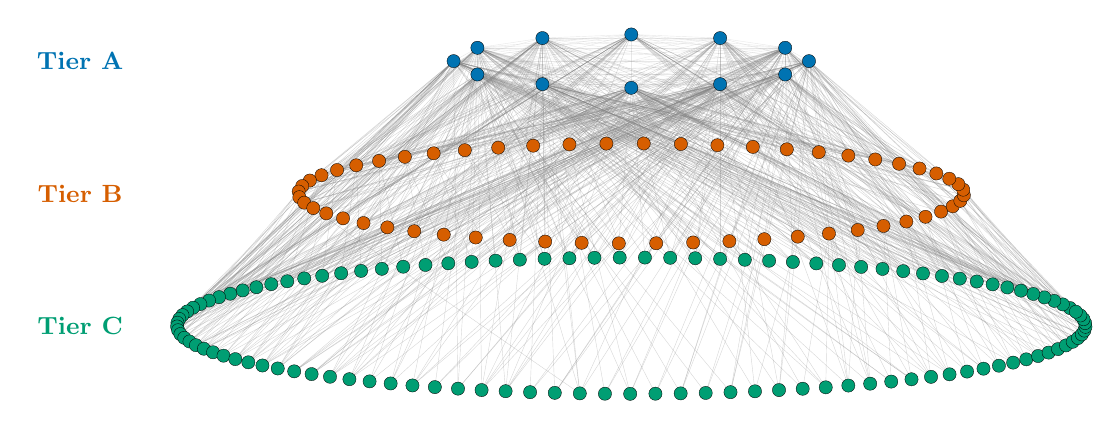
\begin{tikzpicture}[scale=1.4]
  \draw[gray, line width=0.15pt, opacity=0.18] (1.612,1.200) -- (1.396,1.321);
  \draw[gray, line width=0.15pt, opacity=0.18] (1.612,1.200) -- (0.806,1.409);
  \draw[gray, line width=0.15pt, opacity=0.18] (1.612,1.200) -- (0.000,1.442);
  \draw[gray, line width=0.15pt, opacity=0.18] (1.612,1.200) -- (-0.806,1.409);
  \draw[gray, line width=0.15pt, opacity=0.18] (1.612,1.200) -- (-1.396,1.321);
  \draw[gray, line width=0.15pt, opacity=0.18] (1.612,1.200) -- (-1.612,1.200);
  \draw[gray, line width=0.15pt, opacity=0.18] (1.612,1.200) -- (-1.396,1.079);
  \draw[gray, line width=0.15pt, opacity=0.18] (1.612,1.200) -- (-0.806,0.991);
  \draw[gray, line width=0.15pt, opacity=0.18] (1.612,1.200) -- (-0.000,0.958);
  \draw[gray, line width=0.15pt, opacity=0.18] (1.612,1.200) -- (0.806,0.991);
  \draw[gray, line width=0.15pt, opacity=0.18] (1.612,1.200) -- (1.396,1.079);
  \draw[gray, line width=0.15pt, opacity=0.32] (1.612,1.200) -- (1.969,0.343);
  \draw[gray, line width=0.15pt, opacity=0.32] (1.612,1.200) -- (1.411,0.400);
  \draw[gray, line width=0.15pt, opacity=0.32] (1.612,1.200) -- (0.781,0.437);
  \draw[gray, line width=0.15pt, opacity=0.32] (1.612,1.200) -- (-0.226,0.452);
  \draw[gray, line width=0.15pt, opacity=0.32] (1.612,1.200) -- (-0.890,0.433);
  \draw[gray, line width=0.15pt, opacity=0.32] (1.612,1.200) -- (-2.054,0.332);
  \draw[gray, line width=0.15pt, opacity=0.32] (1.612,1.200) -- (-2.669,0.212);
  \draw[gray, line width=0.15pt, opacity=0.32] (1.612,1.200) -- (-2.810,0.165);
  \draw[gray, line width=0.15pt, opacity=0.32] (1.612,1.200) -- (-2.985,0.067);
  \draw[gray, line width=0.15pt, opacity=0.32] (1.612,1.200) -- (-3.017,0.017);
  \draw[gray, line width=0.15pt, opacity=0.32] (1.612,1.200) -- (-2.967,-0.084);
  \draw[gray, line width=0.15pt, opacity=0.32] (1.612,1.200) -- (-2.429,-0.269);
  \draw[gray, line width=0.15pt, opacity=0.32] (1.612,1.200) -- (0.890,-0.433);
  \draw[gray, line width=0.15pt, opacity=0.32] (1.612,1.200) -- (1.207,-0.415);
  \draw[gray, line width=0.15pt, opacity=0.32] (1.612,1.200) -- (1.510,-0.392);
  \draw[gray, line width=0.15pt, opacity=0.32] (1.612,1.200) -- (2.054,-0.332);
  \draw[gray, line width=0.15pt, opacity=0.32] (1.612,1.200) -- (2.810,-0.165);
  \draw[gray, line width=0.15pt, opacity=0.32] (1.612,1.200) -- (3.017,-0.017);
  \draw[gray, line width=0.15pt, opacity=0.32] (1.612,1.200) -- (2.885,0.133);
  \draw[gray, line width=0.15pt, opacity=0.32] (1.612,1.200) -- (3.411,-0.853);
  \draw[gray, line width=0.15pt, opacity=0.32] (1.612,1.200) -- (3.278,-0.825);
  \draw[gray, line width=0.15pt, opacity=0.32] (1.612,1.200) -- (2.818,-0.749);
  \draw[gray, line width=0.15pt, opacity=0.32] (1.612,1.200) -- (2.646,-0.726);
  \draw[gray, line width=0.15pt, opacity=0.32] (1.612,1.200) -- (2.085,-0.667);
  \draw[gray, line width=0.15pt, opacity=0.32] (1.612,1.200) -- (1.884,-0.650);
  \draw[gray, line width=0.15pt, opacity=0.32] (1.612,1.200) -- (0.806,-0.594);
  \draw[gray, line width=0.15pt, opacity=0.32] (1.612,1.200) -- (0.580,-0.588);
  \draw[gray, line width=0.15pt, opacity=0.32] (1.612,1.200) -- (-0.105,-0.582);
  \draw[gray, line width=0.15pt, opacity=0.32] (1.612,1.200) -- (-0.334,-0.584);
  \draw[gray, line width=0.15pt, opacity=0.32] (1.612,1.200) -- (-1.660,-0.634);
  \draw[gray, line width=0.15pt, opacity=0.32] (1.612,1.200) -- (-1.867,-0.649);
  \draw[gray, line width=0.15pt, opacity=0.32] (1.612,1.200) -- (-2.804,-0.747);
  \draw[gray, line width=0.15pt, opacity=0.32] (1.612,1.200) -- (-2.967,-0.771);
  \draw[gray, line width=0.15pt, opacity=0.32] (1.612,1.200) -- (-3.121,-0.797);
  \draw[gray, line width=0.15pt, opacity=0.32] (1.612,1.200) -- (-3.266,-0.823);
  \draw[gray, line width=0.15pt, opacity=0.32] (1.612,1.200) -- (-3.638,-0.910);
  \draw[gray, line width=0.15pt, opacity=0.32] (1.612,1.200) -- (-3.740,-0.941);
  \draw[gray, line width=0.15pt, opacity=0.32] (1.612,1.200) -- (-3.830,-0.972);
  \draw[gray, line width=0.15pt, opacity=0.32] (1.612,1.200) -- (-3.909,-1.004);
  \draw[gray, line width=0.15pt, opacity=0.32] (1.612,1.200) -- (-4.100,-1.139);
  \draw[gray, line width=0.15pt, opacity=0.32] (1.612,1.200) -- (-3.949,-1.377);
  \draw[gray, line width=0.15pt, opacity=0.32] (1.612,1.200) -- (-3.877,-1.409);
  \draw[gray, line width=0.15pt, opacity=0.32] (1.612,1.200) -- (0.448,-1.814);
  \draw[gray, line width=0.15pt, opacity=0.32] (1.612,1.200) -- (0.675,-1.810);
  \draw[gray, line width=0.15pt, opacity=0.32] (1.612,1.200) -- (0.900,-1.803);
  \draw[gray, line width=0.15pt, opacity=0.32] (1.612,1.200) -- (1.340,-1.784);
  \draw[gray, line width=0.15pt, opacity=0.32] (1.612,1.200) -- (1.969,-1.743);
  \draw[gray, line width=0.15pt, opacity=0.32] (1.612,1.200) -- (2.167,-1.726);
  \draw[gray, line width=0.15pt, opacity=0.32] (1.612,1.200) -- (3.335,-1.563);
  \draw[gray, line width=0.15pt, opacity=0.32] (1.612,1.200) -- (3.464,-1.535);
  \draw[gray, line width=0.15pt, opacity=0.32] (1.612,1.200) -- (3.943,-1.379);
  \draw[gray, line width=0.15pt, opacity=0.32] (1.612,1.200) -- (4.004,-1.346);
  \draw[gray, line width=0.15pt, opacity=0.32] (1.612,1.200) -- (4.117,-1.176);
  \draw[gray, line width=0.15pt, opacity=0.32] (1.612,1.200) -- (4.102,-1.141);
  \draw[gray, line width=0.15pt, opacity=0.18] (1.396,1.321) -- (0.806,1.409);
  \draw[gray, line width=0.15pt, opacity=0.18] (1.396,1.321) -- (0.000,1.442);
  \draw[gray, line width=0.15pt, opacity=0.18] (1.396,1.321) -- (-0.806,1.409);
  \draw[gray, line width=0.15pt, opacity=0.18] (1.396,1.321) -- (-1.396,1.321);
  \draw[gray, line width=0.15pt, opacity=0.18] (1.396,1.321) -- (-1.612,1.200);
  \draw[gray, line width=0.15pt, opacity=0.18] (1.396,1.321) -- (-1.396,1.079);
  \draw[gray, line width=0.15pt, opacity=0.18] (1.396,1.321) -- (-0.806,0.991);
  \draw[gray, line width=0.15pt, opacity=0.18] (1.396,1.321) -- (-0.000,0.958);
  \draw[gray, line width=0.15pt, opacity=0.18] (1.396,1.321) -- (0.806,0.991);
  \draw[gray, line width=0.15pt, opacity=0.18] (1.396,1.321) -- (1.396,1.079);
  \draw[gray, line width=0.15pt, opacity=0.32] (1.396,1.321) -- (2.213,0.308);
  \draw[gray, line width=0.15pt, opacity=0.32] (1.396,1.321) -- (1.701,0.374);
  \draw[gray, line width=0.15pt, opacity=0.32] (1.396,1.321) -- (1.411,0.400);
  \draw[gray, line width=0.15pt, opacity=0.32] (1.396,1.321) -- (0.781,0.437);
  \draw[gray, line width=0.15pt, opacity=0.32] (1.396,1.321) -- (0.450,0.448);
  \draw[gray, line width=0.15pt, opacity=0.32] (1.396,1.321) -- (0.113,0.453);
  \draw[gray, line width=0.15pt, opacity=0.32] (1.396,1.321) -- (-0.561,0.445);
  \draw[gray, line width=0.15pt, opacity=0.32] (1.396,1.321) -- (-1.207,0.415);
  \draw[gray, line width=0.15pt, opacity=0.32] (1.396,1.321) -- (-1.510,0.392);
  \draw[gray, line width=0.15pt, opacity=0.32] (1.396,1.321) -- (-1.793,0.364);
  \draw[gray, line width=0.15pt, opacity=0.32] (1.396,1.321) -- (-2.054,0.332);
  \draw[gray, line width=0.15pt, opacity=0.32] (1.396,1.321) -- (-2.495,0.255);
  \draw[gray, line width=0.15pt, opacity=0.32] (1.396,1.321) -- (-2.885,-0.133);
  \draw[gray, line width=0.15pt, opacity=0.32] (1.396,1.321) -- (-2.767,-0.181);
  \draw[gray, line width=0.15pt, opacity=0.32] (1.396,1.321) -- (-2.429,-0.269);
  \draw[gray, line width=0.15pt, opacity=0.32] (1.396,1.321) -- (-1.969,-0.343);
  \draw[gray, line width=0.15pt, opacity=0.32] (1.396,1.321) -- (-1.701,-0.374);
  \draw[gray, line width=0.15pt, opacity=0.32] (1.396,1.321) -- (-1.411,-0.400);
  \draw[gray, line width=0.15pt, opacity=0.32] (1.396,1.321) -- (0.226,-0.452);
  \draw[gray, line width=0.15pt, opacity=0.32] (1.396,1.321) -- (0.561,-0.445);
  \draw[gray, line width=0.15pt, opacity=0.32] (1.396,1.321) -- (3.017,-0.017);
  \draw[gray, line width=0.15pt, opacity=0.32] (1.396,1.321) -- (3.011,0.034);
  \draw[gray, line width=0.15pt, opacity=0.32] (1.396,1.321) -- (3.647,-0.912);
  \draw[gray, line width=0.15pt, opacity=0.32] (1.396,1.321) -- (3.535,-0.882);
  \draw[gray, line width=0.15pt, opacity=0.32] (1.396,1.321) -- (3.134,-0.799);
  \draw[gray, line width=0.15pt, opacity=0.32] (1.396,1.321) -- (2.980,-0.773);
  \draw[gray, line width=0.15pt, opacity=0.32] (1.396,1.321) -- (2.818,-0.749);
  \draw[gray, line width=0.15pt, opacity=0.32] (1.396,1.321) -- (2.646,-0.726);
  \draw[gray, line width=0.15pt, opacity=0.32] (1.396,1.321) -- (2.085,-0.667);
  \draw[gray, line width=0.15pt, opacity=0.32] (1.396,1.321) -- (1.884,-0.650);
  \draw[gray, line width=0.15pt, opacity=0.32] (1.396,1.321) -- (1.466,-0.622);
  \draw[gray, line width=0.15pt, opacity=0.32] (1.396,1.321) -- (1.030,-0.602);
  \draw[gray, line width=0.15pt, opacity=0.32] (1.396,1.321) -- (0.353,-0.584);
  \draw[gray, line width=0.15pt, opacity=0.32] (1.396,1.321) -- (0.124,-0.582);
  \draw[gray, line width=0.15pt, opacity=0.32] (1.396,1.321) -- (-0.561,-0.588);
  \draw[gray, line width=0.15pt, opacity=0.32] (1.396,1.321) -- (-0.787,-0.593);
  \draw[gray, line width=0.15pt, opacity=0.32] (1.396,1.321) -- (-1.011,-0.601);
  \draw[gray, line width=0.15pt, opacity=0.32] (1.396,1.321) -- (-1.231,-0.610);
  \draw[gray, line width=0.15pt, opacity=0.32] (1.396,1.321) -- (-1.448,-0.621);
  \draw[gray, line width=0.15pt, opacity=0.32] (1.396,1.321) -- (-1.867,-0.649);
  \draw[gray, line width=0.15pt, opacity=0.32] (1.396,1.321) -- (-2.451,-0.703);
  \draw[gray, line width=0.15pt, opacity=0.32] (1.396,1.321) -- (-2.632,-0.724);
  \draw[gray, line width=0.15pt, opacity=0.32] (1.396,1.321) -- (-4.117,-1.173);
  \draw[gray, line width=0.15pt, opacity=0.32] (1.396,1.321) -- (-4.120,-1.207);
  \draw[gray, line width=0.15pt, opacity=0.32] (1.396,1.321) -- (-4.111,-1.241);
  \draw[gray, line width=0.15pt, opacity=0.32] (1.396,1.321) -- (-4.090,-1.276);
  \draw[gray, line width=0.15pt, opacity=0.32] (1.396,1.321) -- (-3.949,-1.377);
  \draw[gray, line width=0.15pt, opacity=0.32] (1.396,1.321) -- (-3.877,-1.409);
  \draw[gray, line width=0.15pt, opacity=0.32] (1.396,1.321) -- (-3.592,-1.503);
  \draw[gray, line width=0.15pt, opacity=0.32] (1.396,1.321) -- (-3.474,-1.532);
  \draw[gray, line width=0.15pt, opacity=0.32] (1.396,1.321) -- (-3.346,-1.561);
  \draw[gray, line width=0.15pt, opacity=0.32] (1.396,1.321) -- (-3.058,-1.614);
  \draw[gray, line width=0.15pt, opacity=0.32] (1.396,1.321) -- (-2.900,-1.639);
  \draw[gray, line width=0.15pt, opacity=0.32] (1.396,1.321) -- (-1.985,-1.742);
  \draw[gray, line width=0.15pt, opacity=0.32] (1.396,1.321) -- (-0.918,-1.803);
  \draw[gray, line width=0.15pt, opacity=0.32] (1.396,1.321) -- (-0.694,-1.809);
  \draw[gray, line width=0.15pt, opacity=0.32] (1.396,1.321) -- (-0.239,-1.817);
  \draw[gray, line width=0.15pt, opacity=0.32] (1.396,1.321) -- (-0.010,-1.818);
  \draw[gray, line width=0.15pt, opacity=0.32] (1.396,1.321) -- (3.943,-1.379);
  \draw[gray, line width=0.15pt, opacity=0.32] (1.396,1.321) -- (4.004,-1.346);
  \draw[gray, line width=0.15pt, opacity=0.32] (1.396,1.321) -- (4.052,-1.312);
  \draw[gray, line width=0.15pt, opacity=0.32] (1.396,1.321) -- (4.087,-1.279);
  \draw[gray, line width=0.15pt, opacity=0.18] (0.806,1.409) -- (0.000,1.442);
  \draw[gray, line width=0.15pt, opacity=0.18] (0.806,1.409) -- (-0.806,1.409);
  \draw[gray, line width=0.15pt, opacity=0.18] (0.806,1.409) -- (-1.396,1.321);
  \draw[gray, line width=0.15pt, opacity=0.18] (0.806,1.409) -- (-1.612,1.200);
  \draw[gray, line width=0.15pt, opacity=0.18] (0.806,1.409) -- (-1.396,1.079);
  \draw[gray, line width=0.15pt, opacity=0.18] (0.806,1.409) -- (-0.806,0.991);
  \draw[gray, line width=0.15pt, opacity=0.18] (0.806,1.409) -- (-0.000,0.958);
  \draw[gray, line width=0.15pt, opacity=0.18] (0.806,1.409) -- (0.806,0.991);
  \draw[gray, line width=0.15pt, opacity=0.18] (0.806,1.409) -- (1.396,1.079);
  \draw[gray, line width=0.15pt, opacity=0.32] (0.806,1.409) -- (1.701,0.374);
  \draw[gray, line width=0.15pt, opacity=0.32] (0.806,1.409) -- (1.103,0.422);
  \draw[gray, line width=0.15pt, opacity=0.32] (0.806,1.409) -- (-0.226,0.452);
  \draw[gray, line width=0.15pt, opacity=0.32] (0.806,1.409) -- (-0.890,0.433);
  \draw[gray, line width=0.15pt, opacity=0.32] (0.806,1.409) -- (-1.207,0.415);
  \draw[gray, line width=0.15pt, opacity=0.32] (0.806,1.409) -- (-1.510,0.392);
  \draw[gray, line width=0.15pt, opacity=0.32] (0.806,1.409) -- (-1.793,0.364);
  \draw[gray, line width=0.15pt, opacity=0.32] (0.806,1.409) -- (-2.429,-0.269);
  \draw[gray, line width=0.15pt, opacity=0.32] (0.806,1.409) -- (-1.411,-0.400);
  \draw[gray, line width=0.15pt, opacity=0.32] (0.806,1.409) -- (-1.103,-0.422);
  \draw[gray, line width=0.15pt, opacity=0.32] (0.806,1.409) -- (-0.113,-0.453);
  \draw[gray, line width=0.15pt, opacity=0.32] (0.806,1.409) -- (2.054,-0.332);
  \draw[gray, line width=0.15pt, opacity=0.32] (0.806,1.409) -- (2.288,-0.295);
  \draw[gray, line width=0.15pt, opacity=0.32] (0.806,1.409) -- (2.669,-0.212);
  \draw[gray, line width=0.15pt, opacity=0.32] (0.806,1.409) -- (2.985,-0.067);
  \draw[gray, line width=0.15pt, opacity=0.32] (0.806,1.409) -- (3.017,-0.017);
  \draw[gray, line width=0.15pt, opacity=0.32] (0.806,1.409) -- (2.767,0.181);
  \draw[gray, line width=0.15pt, opacity=0.32] (0.806,1.409) -- (3.134,-0.799);
  \draw[gray, line width=0.15pt, opacity=0.32] (0.806,1.409) -- (2.980,-0.773);
  \draw[gray, line width=0.15pt, opacity=0.32] (0.806,1.409) -- (2.467,-0.705);
  \draw[gray, line width=0.15pt, opacity=0.32] (0.806,1.409) -- (2.279,-0.685);
  \draw[gray, line width=0.15pt, opacity=0.32] (0.806,1.409) -- (0.806,-0.594);
  \draw[gray, line width=0.15pt, opacity=0.32] (0.806,1.409) -- (0.580,-0.588);
  \draw[gray, line width=0.15pt, opacity=0.32] (0.806,1.409) -- (-0.105,-0.582);
  \draw[gray, line width=0.15pt, opacity=0.32] (0.806,1.409) -- (-0.334,-0.584);
  \draw[gray, line width=0.15pt, opacity=0.32] (0.806,1.409) -- (-0.561,-0.588);
  \draw[gray, line width=0.15pt, opacity=0.32] (0.806,1.409) -- (-1.231,-0.610);
  \draw[gray, line width=0.15pt, opacity=0.32] (0.806,1.409) -- (-1.448,-0.621);
  \draw[gray, line width=0.15pt, opacity=0.32] (0.806,1.409) -- (-3.949,-1.377);
  \draw[gray, line width=0.15pt, opacity=0.32] (0.806,1.409) -- (-3.877,-1.409);
  \draw[gray, line width=0.15pt, opacity=0.32] (0.806,1.409) -- (-3.058,-1.614);
  \draw[gray, line width=0.15pt, opacity=0.32] (0.806,1.409) -- (-2.900,-1.639);
  \draw[gray, line width=0.15pt, opacity=0.32] (0.806,1.409) -- (-2.733,-1.663);
  \draw[gray, line width=0.15pt, opacity=0.32] (0.806,1.409) -- (-2.557,-1.685);
  \draw[gray, line width=0.15pt, opacity=0.32] (0.806,1.409) -- (-1.358,-1.784);
  \draw[gray, line width=0.15pt, opacity=0.32] (0.806,1.409) -- (-1.140,-1.794);
  \draw[gray, line width=0.15pt, opacity=0.32] (0.806,1.409) -- (1.969,-1.743);
  \draw[gray, line width=0.15pt, opacity=0.32] (0.806,1.409) -- (2.167,-1.726);
  \draw[gray, line width=0.15pt, opacity=0.32] (0.806,1.409) -- (2.358,-1.707);
  \draw[gray, line width=0.15pt, opacity=0.32] (0.806,1.409) -- (2.542,-1.686);
  \draw[gray, line width=0.15pt, opacity=0.32] (0.806,1.409) -- (3.046,-1.616);
  \draw[gray, line width=0.15pt, opacity=0.32] (0.806,1.409) -- (3.195,-1.590);
  \draw[gray, line width=0.15pt, opacity=0.32] (0.806,1.409) -- (3.786,-1.444);
  \draw[gray, line width=0.15pt, opacity=0.32] (0.806,1.409) -- (3.871,-1.412);
  \draw[gray, line width=0.15pt, opacity=0.32] (0.806,1.409) -- (3.943,-1.379);
  \draw[gray, line width=0.15pt, opacity=0.32] (0.806,1.409) -- (4.004,-1.346);
  \draw[gray, line width=0.15pt, opacity=0.32] (0.806,1.409) -- (4.074,-1.107);
  \draw[gray, line width=0.15pt, opacity=0.32] (0.806,1.409) -- (4.033,-1.073);
  \draw[gray, line width=0.15pt, opacity=0.18] (0.000,1.442) -- (-0.806,1.409);
  \draw[gray, line width=0.15pt, opacity=0.18] (0.000,1.442) -- (-1.396,1.321);
  \draw[gray, line width=0.15pt, opacity=0.18] (0.000,1.442) -- (-1.612,1.200);
  \draw[gray, line width=0.15pt, opacity=0.18] (0.000,1.442) -- (-1.396,1.079);
  \draw[gray, line width=0.15pt, opacity=0.18] (0.000,1.442) -- (-0.806,0.991);
  \draw[gray, line width=0.15pt, opacity=0.18] (0.000,1.442) -- (-0.000,0.958);
  \draw[gray, line width=0.15pt, opacity=0.18] (0.000,1.442) -- (0.806,0.991);
  \draw[gray, line width=0.15pt, opacity=0.18] (0.000,1.442) -- (1.396,1.079);
  \draw[gray, line width=0.15pt, opacity=0.32] (0.000,1.442) -- (1.701,0.374);
  \draw[gray, line width=0.15pt, opacity=0.32] (0.000,1.442) -- (1.411,0.400);
  \draw[gray, line width=0.15pt, opacity=0.32] (0.000,1.442) -- (-1.207,0.415);
  \draw[gray, line width=0.15pt, opacity=0.32] (0.000,1.442) -- (-1.510,0.392);
  \draw[gray, line width=0.15pt, opacity=0.32] (0.000,1.442) -- (-2.495,0.255);
  \draw[gray, line width=0.15pt, opacity=0.32] (0.000,1.442) -- (-2.669,0.212);
  \draw[gray, line width=0.15pt, opacity=0.32] (0.000,1.442) -- (-3.017,0.017);
  \draw[gray, line width=0.15pt, opacity=0.32] (0.000,1.442) -- (-3.011,-0.034);
  \draw[gray, line width=0.15pt, opacity=0.32] (0.000,1.442) -- (-2.967,-0.084);
  \draw[gray, line width=0.15pt, opacity=0.32] (0.000,1.442) -- (-1.969,-0.343);
  \draw[gray, line width=0.15pt, opacity=0.32] (0.000,1.442) -- (-1.701,-0.374);
  \draw[gray, line width=0.15pt, opacity=0.32] (0.000,1.442) -- (-1.103,-0.422);
  \draw[gray, line width=0.15pt, opacity=0.32] (0.000,1.442) -- (2.810,-0.165);
  \draw[gray, line width=0.15pt, opacity=0.32] (0.000,1.442) -- (2.885,0.133);
  \draw[gray, line width=0.15pt, opacity=0.32] (0.000,1.442) -- (2.767,0.181);
  \draw[gray, line width=0.15pt, opacity=0.32] (0.000,1.442) -- (3.134,-0.799);
  \draw[gray, line width=0.15pt, opacity=0.32] (0.000,1.442) -- (2.980,-0.773);
  \draw[gray, line width=0.15pt, opacity=0.32] (0.000,1.442) -- (2.818,-0.749);
  \draw[gray, line width=0.15pt, opacity=0.32] (0.000,1.442) -- (2.646,-0.726);
  \draw[gray, line width=0.15pt, opacity=0.32] (0.000,1.442) -- (-0.787,-0.593);
  \draw[gray, line width=0.15pt, opacity=0.32] (0.000,1.442) -- (-2.451,-0.703);
  \draw[gray, line width=0.15pt, opacity=0.32] (0.000,1.442) -- (-2.632,-0.724);
  \draw[gray, line width=0.15pt, opacity=0.32] (0.000,1.442) -- (-2.967,-0.771);
  \draw[gray, line width=0.15pt, opacity=0.32] (0.000,1.442) -- (-3.830,-0.972);
  \draw[gray, line width=0.15pt, opacity=0.32] (0.000,1.442) -- (-3.909,-1.004);
  \draw[gray, line width=0.15pt, opacity=0.32] (0.000,1.442) -- (-3.975,-1.037);
  \draw[gray, line width=0.15pt, opacity=0.32] (0.000,1.442) -- (-4.029,-1.071);
  \draw[gray, line width=0.15pt, opacity=0.32] (0.000,1.442) -- (-4.071,-1.104);
  \draw[gray, line width=0.15pt, opacity=0.32] (0.000,1.442) -- (-4.100,-1.139);
  \draw[gray, line width=0.15pt, opacity=0.32] (0.000,1.442) -- (-3.592,-1.503);
  \draw[gray, line width=0.15pt, opacity=0.32] (0.000,1.442) -- (-3.474,-1.532);
  \draw[gray, line width=0.15pt, opacity=0.32] (0.000,1.442) -- (-3.346,-1.561);
  \draw[gray, line width=0.15pt, opacity=0.32] (0.000,1.442) -- (-3.207,-1.588);
  \draw[gray, line width=0.15pt, opacity=0.32] (0.000,1.442) -- (-2.733,-1.663);
  \draw[gray, line width=0.15pt, opacity=0.32] (0.000,1.442) -- (-2.557,-1.685);
  \draw[gray, line width=0.15pt, opacity=0.32] (0.000,1.442) -- (-1.985,-1.742);
  \draw[gray, line width=0.15pt, opacity=0.32] (0.000,1.442) -- (3.335,-1.563);
  \draw[gray, line width=0.15pt, opacity=0.32] (0.000,1.442) -- (3.464,-1.535);
  \draw[gray, line width=0.15pt, opacity=0.32] (0.000,1.442) -- (4.117,-1.176);
  \draw[gray, line width=0.15pt, opacity=0.32] (0.000,1.442) -- (4.102,-1.141);
  \draw[gray, line width=0.15pt, opacity=0.32] (0.000,1.442) -- (4.074,-1.107);
  \draw[gray, line width=0.15pt, opacity=0.32] (0.000,1.442) -- (4.033,-1.073);
  \draw[gray, line width=0.15pt, opacity=0.18] (-0.806,1.409) -- (-1.396,1.321);
  \draw[gray, line width=0.15pt, opacity=0.18] (-0.806,1.409) -- (-1.612,1.200);
  \draw[gray, line width=0.15pt, opacity=0.18] (-0.806,1.409) -- (-1.396,1.079);
  \draw[gray, line width=0.15pt, opacity=0.18] (-0.806,1.409) -- (-0.806,0.991);
  \draw[gray, line width=0.15pt, opacity=0.18] (-0.806,1.409) -- (-0.000,0.958);
  \draw[gray, line width=0.15pt, opacity=0.18] (-0.806,1.409) -- (0.806,0.991);
  \draw[gray, line width=0.15pt, opacity=0.18] (-0.806,1.409) -- (1.396,1.079);
  \draw[gray, line width=0.15pt, opacity=0.32] (-0.806,1.409) -- (2.213,0.308);
  \draw[gray, line width=0.15pt, opacity=0.32] (-0.806,1.409) -- (0.450,0.448);
  \draw[gray, line width=0.15pt, opacity=0.32] (-0.806,1.409) -- (0.113,0.453);
  \draw[gray, line width=0.15pt, opacity=0.32] (-0.806,1.409) -- (-1.207,0.415);
  \draw[gray, line width=0.15pt, opacity=0.32] (-0.806,1.409) -- (-1.510,0.392);
  \draw[gray, line width=0.15pt, opacity=0.32] (-0.806,1.409) -- (-2.985,0.067);
  \draw[gray, line width=0.15pt, opacity=0.32] (-0.806,1.409) -- (-3.017,0.017);
  \draw[gray, line width=0.15pt, opacity=0.32] (-0.806,1.409) -- (-3.011,-0.034);
  \draw[gray, line width=0.15pt, opacity=0.32] (-0.806,1.409) -- (-2.967,-0.084);
  \draw[gray, line width=0.15pt, opacity=0.32] (-0.806,1.409) -- (-2.767,-0.181);
  \draw[gray, line width=0.15pt, opacity=0.32] (-0.806,1.409) -- (-2.615,-0.226);
  \draw[gray, line width=0.15pt, opacity=0.32] (-0.806,1.409) -- (-1.969,-0.343);
  \draw[gray, line width=0.15pt, opacity=0.32] (-0.806,1.409) -- (-1.701,-0.374);
  \draw[gray, line width=0.15pt, opacity=0.32] (-0.806,1.409) -- (-1.103,-0.422);
  \draw[gray, line width=0.15pt, opacity=0.32] (-0.806,1.409) -- (-0.781,-0.437);
  \draw[gray, line width=0.15pt, opacity=0.32] (-0.806,1.409) -- (-0.113,-0.453);
  \draw[gray, line width=0.15pt, opacity=0.32] (-0.806,1.409) -- (0.561,-0.445);
  \draw[gray, line width=0.15pt, opacity=0.32] (-0.806,1.409) -- (1.510,-0.392);
  \draw[gray, line width=0.15pt, opacity=0.32] (-0.806,1.409) -- (2.669,-0.212);
  \draw[gray, line width=0.15pt, opacity=0.32] (-0.806,1.409) -- (2.916,-0.117);
  \draw[gray, line width=0.15pt, opacity=0.32] (-0.806,1.409) -- (2.967,0.084);
  \draw[gray, line width=0.15pt, opacity=0.32] (-0.806,1.409) -- (3.647,-0.912);
  \draw[gray, line width=0.15pt, opacity=0.32] (-0.806,1.409) -- (3.535,-0.882);
  \draw[gray, line width=0.15pt, opacity=0.32] (-0.806,1.409) -- (1.678,-0.635);
  \draw[gray, line width=0.15pt, opacity=0.32] (-0.806,1.409) -- (1.466,-0.622);
  \draw[gray, line width=0.15pt, opacity=0.32] (-0.806,1.409) -- (1.250,-0.611);
  \draw[gray, line width=0.15pt, opacity=0.32] (-0.806,1.409) -- (1.030,-0.602);
  \draw[gray, line width=0.15pt, opacity=0.32] (-0.806,1.409) -- (-0.787,-0.593);
  \draw[gray, line width=0.15pt, opacity=0.32] (-0.806,1.409) -- (-1.011,-0.601);
  \draw[gray, line width=0.15pt, opacity=0.32] (-0.806,1.409) -- (-3.638,-0.910);
  \draw[gray, line width=0.15pt, opacity=0.32] (-0.806,1.409) -- (-3.740,-0.941);
  \draw[gray, line width=0.15pt, opacity=0.32] (-0.806,1.409) -- (-3.830,-0.972);
  \draw[gray, line width=0.15pt, opacity=0.32] (-0.806,1.409) -- (-3.909,-1.004);
  \draw[gray, line width=0.15pt, opacity=0.32] (-0.806,1.409) -- (-3.975,-1.037);
  \draw[gray, line width=0.15pt, opacity=0.32] (-0.806,1.409) -- (-4.029,-1.071);
  \draw[gray, line width=0.15pt, opacity=0.32] (-0.806,1.409) -- (-4.071,-1.104);
  \draw[gray, line width=0.15pt, opacity=0.32] (-0.806,1.409) -- (-4.111,-1.241);
  \draw[gray, line width=0.15pt, opacity=0.32] (-0.806,1.409) -- (-4.090,-1.276);
  \draw[gray, line width=0.15pt, opacity=0.32] (-0.806,1.409) -- (-4.055,-1.310);
  \draw[gray, line width=0.15pt, opacity=0.32] (-0.806,1.409) -- (-4.008,-1.343);
  \draw[gray, line width=0.15pt, opacity=0.32] (-0.806,1.409) -- (-3.592,-1.503);
  \draw[gray, line width=0.15pt, opacity=0.32] (-0.806,1.409) -- (-3.474,-1.532);
  \draw[gray, line width=0.15pt, opacity=0.32] (-0.806,1.409) -- (-3.346,-1.561);
  \draw[gray, line width=0.15pt, opacity=0.32] (-0.806,1.409) -- (-3.207,-1.588);
  \draw[gray, line width=0.15pt, opacity=0.32] (-0.806,1.409) -- (-2.733,-1.663);
  \draw[gray, line width=0.15pt, opacity=0.32] (-0.806,1.409) -- (-2.557,-1.685);
  \draw[gray, line width=0.15pt, opacity=0.32] (-0.806,1.409) -- (-2.183,-1.724);
  \draw[gray, line width=0.15pt, opacity=0.32] (-0.806,1.409) -- (-1.358,-1.784);
  \draw[gray, line width=0.15pt, opacity=0.32] (-0.806,1.409) -- (-1.140,-1.794);
  \draw[gray, line width=0.15pt, opacity=0.32] (-0.806,1.409) -- (-0.467,-1.814);
  \draw[gray, line width=0.15pt, opacity=0.32] (-0.806,1.409) -- (-0.239,-1.817);
  \draw[gray, line width=0.15pt, opacity=0.32] (-0.806,1.409) -- (-0.010,-1.818);
  \draw[gray, line width=0.15pt, opacity=0.32] (-0.806,1.409) -- (1.122,-1.795);
  \draw[gray, line width=0.15pt, opacity=0.32] (-0.806,1.409) -- (1.340,-1.784);
  \draw[gray, line width=0.15pt, opacity=0.32] (-0.806,1.409) -- (3.195,-1.590);
  \draw[gray, line width=0.15pt, opacity=0.32] (-0.806,1.409) -- (3.690,-1.475);
  \draw[gray, line width=0.15pt, opacity=0.32] (-0.806,1.409) -- (4.110,-1.244);
  \draw[gray, line width=0.15pt, opacity=0.32] (-0.806,1.409) -- (4.120,-1.210);
  \draw[gray, line width=0.15pt, opacity=0.18] (-1.396,1.321) -- (-1.612,1.200);
  \draw[gray, line width=0.15pt, opacity=0.18] (-1.396,1.321) -- (-1.396,1.079);
  \draw[gray, line width=0.15pt, opacity=0.18] (-1.396,1.321) -- (-0.806,0.991);
  \draw[gray, line width=0.15pt, opacity=0.18] (-1.396,1.321) -- (-0.000,0.958);
  \draw[gray, line width=0.15pt, opacity=0.18] (-1.396,1.321) -- (0.806,0.991);
  \draw[gray, line width=0.15pt, opacity=0.18] (-1.396,1.321) -- (1.396,1.079);
  \draw[gray, line width=0.15pt, opacity=0.32] (-1.396,1.321) -- (2.615,0.226);
  \draw[gray, line width=0.15pt, opacity=0.32] (-1.396,1.321) -- (1.969,0.343);
  \draw[gray, line width=0.15pt, opacity=0.32] (-1.396,1.321) -- (1.701,0.374);
  \draw[gray, line width=0.15pt, opacity=0.32] (-1.396,1.321) -- (1.411,0.400);
  \draw[gray, line width=0.15pt, opacity=0.32] (-1.396,1.321) -- (1.103,0.422);
  \draw[gray, line width=0.15pt, opacity=0.32] (-1.396,1.321) -- (0.781,0.437);
  \draw[gray, line width=0.15pt, opacity=0.32] (-1.396,1.321) -- (0.113,0.453);
  \draw[gray, line width=0.15pt, opacity=0.32] (-1.396,1.321) -- (-1.207,0.415);
  \draw[gray, line width=0.15pt, opacity=0.32] (-1.396,1.321) -- (-1.510,0.392);
  \draw[gray, line width=0.15pt, opacity=0.32] (-1.396,1.321) -- (-2.985,0.067);
  \draw[gray, line width=0.15pt, opacity=0.32] (-1.396,1.321) -- (-3.011,-0.034);
  \draw[gray, line width=0.15pt, opacity=0.32] (-1.396,1.321) -- (-2.967,-0.084);
  \draw[gray, line width=0.15pt, opacity=0.32] (-1.396,1.321) -- (-2.767,-0.181);
  \draw[gray, line width=0.15pt, opacity=0.32] (-1.396,1.321) -- (-2.213,-0.308);
  \draw[gray, line width=0.15pt, opacity=0.32] (-1.396,1.321) -- (-1.969,-0.343);
  \draw[gray, line width=0.15pt, opacity=0.32] (-1.396,1.321) -- (-1.701,-0.374);
  \draw[gray, line width=0.15pt, opacity=0.32] (-1.396,1.321) -- (-0.113,-0.453);
  \draw[gray, line width=0.15pt, opacity=0.32] (-1.396,1.321) -- (0.561,-0.445);
  \draw[gray, line width=0.15pt, opacity=0.32] (-1.396,1.321) -- (0.890,-0.433);
  \draw[gray, line width=0.15pt, opacity=0.32] (-1.396,1.321) -- (2.054,-0.332);
  \draw[gray, line width=0.15pt, opacity=0.32] (-1.396,1.321) -- (2.288,-0.295);
  \draw[gray, line width=0.15pt, opacity=0.32] (-1.396,1.321) -- (3.980,-1.040);
  \draw[gray, line width=0.15pt, opacity=0.32] (-1.396,1.321) -- (3.915,-1.007);
  \draw[gray, line width=0.15pt, opacity=0.32] (-1.396,1.321) -- (3.411,-0.853);
  \draw[gray, line width=0.15pt, opacity=0.32] (-1.396,1.321) -- (3.278,-0.825);
  \draw[gray, line width=0.15pt, opacity=0.32] (-1.396,1.321) -- (3.134,-0.799);
  \draw[gray, line width=0.15pt, opacity=0.32] (-1.396,1.321) -- (2.980,-0.773);
  \draw[gray, line width=0.15pt, opacity=0.32] (-1.396,1.321) -- (2.818,-0.749);
  \draw[gray, line width=0.15pt, opacity=0.32] (-1.396,1.321) -- (2.646,-0.726);
  \draw[gray, line width=0.15pt, opacity=0.32] (-1.396,1.321) -- (2.467,-0.705);
  \draw[gray, line width=0.15pt, opacity=0.32] (-1.396,1.321) -- (2.279,-0.685);
  \draw[gray, line width=0.15pt, opacity=0.32] (-1.396,1.321) -- (2.085,-0.667);
  \draw[gray, line width=0.15pt, opacity=0.32] (-1.396,1.321) -- (1.884,-0.650);
  \draw[gray, line width=0.15pt, opacity=0.32] (-1.396,1.321) -- (1.250,-0.611);
  \draw[gray, line width=0.15pt, opacity=0.32] (-1.396,1.321) -- (1.030,-0.602);
  \draw[gray, line width=0.15pt, opacity=0.32] (-1.396,1.321) -- (-0.561,-0.588);
  \draw[gray, line width=0.15pt, opacity=0.32] (-1.396,1.321) -- (-0.787,-0.593);
  \draw[gray, line width=0.15pt, opacity=0.32] (-1.396,1.321) -- (-1.011,-0.601);
  \draw[gray, line width=0.15pt, opacity=0.32] (-1.396,1.321) -- (-3.638,-0.910);
  \draw[gray, line width=0.15pt, opacity=0.32] (-1.396,1.321) -- (-3.740,-0.941);
  \draw[gray, line width=0.15pt, opacity=0.32] (-1.396,1.321) -- (-3.975,-1.037);
  \draw[gray, line width=0.15pt, opacity=0.32] (-1.396,1.321) -- (-4.029,-1.071);
  \draw[gray, line width=0.15pt, opacity=0.32] (-1.396,1.321) -- (-4.071,-1.104);
  \draw[gray, line width=0.15pt, opacity=0.32] (-1.396,1.321) -- (-4.111,-1.241);
  \draw[gray, line width=0.15pt, opacity=0.32] (-1.396,1.321) -- (-4.090,-1.276);
  \draw[gray, line width=0.15pt, opacity=0.32] (-1.396,1.321) -- (-3.794,-1.441);
  \draw[gray, line width=0.15pt, opacity=0.32] (-1.396,1.321) -- (-3.699,-1.472);
  \draw[gray, line width=0.15pt, opacity=0.32] (-1.396,1.321) -- (-3.592,-1.503);
  \draw[gray, line width=0.15pt, opacity=0.32] (-1.396,1.321) -- (-3.474,-1.532);
  \draw[gray, line width=0.15pt, opacity=0.32] (-1.396,1.321) -- (-3.346,-1.561);
  \draw[gray, line width=0.15pt, opacity=0.32] (-1.396,1.321) -- (-3.207,-1.588);
  \draw[gray, line width=0.15pt, opacity=0.32] (-1.396,1.321) -- (-1.358,-1.784);
  \draw[gray, line width=0.15pt, opacity=0.32] (-1.396,1.321) -- (-1.140,-1.794);
  \draw[gray, line width=0.15pt, opacity=0.32] (-1.396,1.321) -- (-0.467,-1.814);
  \draw[gray, line width=0.15pt, opacity=0.32] (-1.396,1.321) -- (-0.010,-1.818);
  \draw[gray, line width=0.15pt, opacity=0.32] (-1.396,1.321) -- (0.219,-1.817);
  \draw[gray, line width=0.15pt, opacity=0.32] (-1.396,1.321) -- (0.448,-1.814);
  \draw[gray, line width=0.15pt, opacity=0.32] (-1.396,1.321) -- (1.969,-1.743);
  \draw[gray, line width=0.15pt, opacity=0.32] (-1.396,1.321) -- (2.167,-1.726);
  \draw[gray, line width=0.15pt, opacity=0.32] (-1.396,1.321) -- (2.542,-1.686);
  \draw[gray, line width=0.15pt, opacity=0.18] (-1.612,1.200) -- (-1.396,1.079);
  \draw[gray, line width=0.15pt, opacity=0.18] (-1.612,1.200) -- (-0.806,0.991);
  \draw[gray, line width=0.15pt, opacity=0.18] (-1.612,1.200) -- (-0.000,0.958);
  \draw[gray, line width=0.15pt, opacity=0.18] (-1.612,1.200) -- (0.806,0.991);
  \draw[gray, line width=0.15pt, opacity=0.18] (-1.612,1.200) -- (1.396,1.079);
  \draw[gray, line width=0.15pt, opacity=0.32] (-1.612,1.200) -- (2.615,0.226);
  \draw[gray, line width=0.15pt, opacity=0.32] (-1.612,1.200) -- (1.969,0.343);
  \draw[gray, line width=0.15pt, opacity=0.32] (-1.612,1.200) -- (1.701,0.374);
  \draw[gray, line width=0.15pt, opacity=0.32] (-1.612,1.200) -- (0.450,0.448);
  \draw[gray, line width=0.15pt, opacity=0.32] (-1.612,1.200) -- (-2.495,0.255);
  \draw[gray, line width=0.15pt, opacity=0.32] (-1.612,1.200) -- (-2.916,0.117);
  \draw[gray, line width=0.15pt, opacity=0.32] (-1.612,1.200) -- (-3.017,0.017);
  \draw[gray, line width=0.15pt, opacity=0.32] (-1.612,1.200) -- (-3.011,-0.034);
  \draw[gray, line width=0.15pt, opacity=0.32] (-1.612,1.200) -- (-2.885,-0.133);
  \draw[gray, line width=0.15pt, opacity=0.32] (-1.612,1.200) -- (-2.767,-0.181);
  \draw[gray, line width=0.15pt, opacity=0.32] (-1.612,1.200) -- (-2.429,-0.269);
  \draw[gray, line width=0.15pt, opacity=0.32] (-1.612,1.200) -- (-0.450,-0.448);
  \draw[gray, line width=0.15pt, opacity=0.32] (-1.612,1.200) -- (1.207,-0.415);
  \draw[gray, line width=0.15pt, opacity=0.32] (-1.612,1.200) -- (2.288,-0.295);
  \draw[gray, line width=0.15pt, opacity=0.32] (-1.612,1.200) -- (2.985,-0.067);
  \draw[gray, line width=0.15pt, opacity=0.32] (-1.612,1.200) -- (3.017,-0.017);
  \draw[gray, line width=0.15pt, opacity=0.32] (-1.612,1.200) -- (3.011,0.034);
  \draw[gray, line width=0.15pt, opacity=0.32] (-1.612,1.200) -- (2.967,0.084);
  \draw[gray, line width=0.15pt, opacity=0.32] (-1.612,1.200) -- (3.980,-1.040);
  \draw[gray, line width=0.15pt, opacity=0.32] (-1.612,1.200) -- (3.915,-1.007);
  \draw[gray, line width=0.15pt, opacity=0.32] (-1.612,1.200) -- (3.278,-0.825);
  \draw[gray, line width=0.15pt, opacity=0.32] (-1.612,1.200) -- (3.134,-0.799);
  \draw[gray, line width=0.15pt, opacity=0.32] (-1.612,1.200) -- (2.980,-0.773);
  \draw[gray, line width=0.15pt, opacity=0.32] (-1.612,1.200) -- (1.678,-0.635);
  \draw[gray, line width=0.15pt, opacity=0.32] (-1.612,1.200) -- (1.466,-0.622);
  \draw[gray, line width=0.15pt, opacity=0.32] (-1.612,1.200) -- (-2.451,-0.703);
  \draw[gray, line width=0.15pt, opacity=0.32] (-1.612,1.200) -- (-2.632,-0.724);
  \draw[gray, line width=0.15pt, opacity=0.32] (-1.612,1.200) -- (-3.401,-0.851);
  \draw[gray, line width=0.15pt, opacity=0.32] (-1.612,1.200) -- (-3.525,-0.880);
  \draw[gray, line width=0.15pt, opacity=0.32] (-1.612,1.200) -- (-3.830,-0.972);
  \draw[gray, line width=0.15pt, opacity=0.32] (-1.612,1.200) -- (-3.909,-1.004);
  \draw[gray, line width=0.15pt, opacity=0.32] (-1.612,1.200) -- (-3.975,-1.037);
  \draw[gray, line width=0.15pt, opacity=0.32] (-1.612,1.200) -- (-4.029,-1.071);
  \draw[gray, line width=0.15pt, opacity=0.32] (-1.612,1.200) -- (-4.117,-1.173);
  \draw[gray, line width=0.15pt, opacity=0.32] (-1.612,1.200) -- (-4.120,-1.207);
  \draw[gray, line width=0.15pt, opacity=0.32] (-1.612,1.200) -- (-4.111,-1.241);
  \draw[gray, line width=0.15pt, opacity=0.32] (-1.612,1.200) -- (-4.090,-1.276);
  \draw[gray, line width=0.15pt, opacity=0.32] (-1.612,1.200) -- (-3.949,-1.377);
  \draw[gray, line width=0.15pt, opacity=0.32] (-1.612,1.200) -- (-3.877,-1.409);
  \draw[gray, line width=0.15pt, opacity=0.32] (-1.612,1.200) -- (-1.572,-1.771);
  \draw[gray, line width=0.15pt, opacity=0.32] (-1.612,1.200) -- (0.675,-1.810);
  \draw[gray, line width=0.15pt, opacity=0.32] (-1.612,1.200) -- (0.900,-1.803);
  \draw[gray, line width=0.15pt, opacity=0.32] (-1.612,1.200) -- (2.358,-1.707);
  \draw[gray, line width=0.15pt, opacity=0.32] (-1.612,1.200) -- (2.542,-1.686);
  \draw[gray, line width=0.15pt, opacity=0.32] (-1.612,1.200) -- (3.786,-1.444);
  \draw[gray, line width=0.15pt, opacity=0.32] (-1.612,1.200) -- (3.871,-1.412);
  \draw[gray, line width=0.15pt, opacity=0.32] (-1.612,1.200) -- (3.943,-1.379);
  \draw[gray, line width=0.15pt, opacity=0.32] (-1.612,1.200) -- (4.004,-1.346);
  \draw[gray, line width=0.15pt, opacity=0.32] (-1.612,1.200) -- (4.052,-1.312);
  \draw[gray, line width=0.15pt, opacity=0.32] (-1.612,1.200) -- (4.087,-1.279);
  \draw[gray, line width=0.15pt, opacity=0.32] (-1.612,1.200) -- (4.120,-1.210);
  \draw[gray, line width=0.15pt, opacity=0.18] (-1.396,1.079) -- (-0.806,0.991);
  \draw[gray, line width=0.15pt, opacity=0.18] (-1.396,1.079) -- (-0.000,0.958);
  \draw[gray, line width=0.15pt, opacity=0.18] (-1.396,1.079) -- (0.806,0.991);
  \draw[gray, line width=0.15pt, opacity=0.18] (-1.396,1.079) -- (1.396,1.079);
  \draw[gray, line width=0.15pt, opacity=0.32] (-1.396,1.079) -- (2.615,0.226);
  \draw[gray, line width=0.15pt, opacity=0.32] (-1.396,1.079) -- (1.103,0.422);
  \draw[gray, line width=0.15pt, opacity=0.32] (-1.396,1.079) -- (0.781,0.437);
  \draw[gray, line width=0.15pt, opacity=0.32] (-1.396,1.079) -- (0.113,0.453);
  \draw[gray, line width=0.15pt, opacity=0.32] (-1.396,1.079) -- (-0.890,0.433);
  \draw[gray, line width=0.15pt, opacity=0.32] (-1.396,1.079) -- (-1.510,0.392);
  \draw[gray, line width=0.15pt, opacity=0.32] (-1.396,1.079) -- (-1.793,0.364);
  \draw[gray, line width=0.15pt, opacity=0.32] (-1.396,1.079) -- (-2.288,0.295);
  \draw[gray, line width=0.15pt, opacity=0.32] (-1.396,1.079) -- (-2.916,0.117);
  \draw[gray, line width=0.15pt, opacity=0.32] (-1.396,1.079) -- (-3.017,0.017);
  \draw[gray, line width=0.15pt, opacity=0.32] (-1.396,1.079) -- (-2.615,-0.226);
  \draw[gray, line width=0.15pt, opacity=0.32] (-1.396,1.079) -- (-2.429,-0.269);
  \draw[gray, line width=0.15pt, opacity=0.32] (-1.396,1.079) -- (-2.213,-0.308);
  \draw[gray, line width=0.15pt, opacity=0.32] (-1.396,1.079) -- (-1.969,-0.343);
  \draw[gray, line width=0.15pt, opacity=0.32] (-1.396,1.079) -- (-1.701,-0.374);
  \draw[gray, line width=0.15pt, opacity=0.32] (-1.396,1.079) -- (-1.103,-0.422);
  \draw[gray, line width=0.15pt, opacity=0.32] (-1.396,1.079) -- (-0.781,-0.437);
  \draw[gray, line width=0.15pt, opacity=0.32] (-1.396,1.079) -- (-0.450,-0.448);
  \draw[gray, line width=0.15pt, opacity=0.32] (-1.396,1.079) -- (1.793,-0.364);
  \draw[gray, line width=0.15pt, opacity=0.32] (-1.396,1.079) -- (2.288,-0.295);
  \draw[gray, line width=0.15pt, opacity=0.32] (-1.396,1.079) -- (2.495,-0.255);
  \draw[gray, line width=0.15pt, opacity=0.32] (-1.396,1.079) -- (2.810,-0.165);
  \draw[gray, line width=0.15pt, opacity=0.32] (-1.396,1.079) -- (3.011,0.034);
  \draw[gray, line width=0.15pt, opacity=0.32] (-1.396,1.079) -- (3.980,-1.040);
  \draw[gray, line width=0.15pt, opacity=0.32] (-1.396,1.079) -- (3.915,-1.007);
  \draw[gray, line width=0.15pt, opacity=0.32] (-1.396,1.079) -- (2.467,-0.705);
  \draw[gray, line width=0.15pt, opacity=0.32] (-1.396,1.079) -- (2.279,-0.685);
  \draw[gray, line width=0.15pt, opacity=0.32] (-1.396,1.079) -- (2.085,-0.667);
  \draw[gray, line width=0.15pt, opacity=0.32] (-1.396,1.079) -- (1.884,-0.650);
  \draw[gray, line width=0.15pt, opacity=0.32] (-1.396,1.079) -- (1.250,-0.611);
  \draw[gray, line width=0.15pt, opacity=0.32] (-1.396,1.079) -- (1.030,-0.602);
  \draw[gray, line width=0.15pt, opacity=0.32] (-1.396,1.079) -- (-0.105,-0.582);
  \draw[gray, line width=0.15pt, opacity=0.32] (-1.396,1.079) -- (-0.334,-0.584);
  \draw[gray, line width=0.15pt, opacity=0.32] (-1.396,1.079) -- (-0.787,-0.593);
  \draw[gray, line width=0.15pt, opacity=0.32] (-1.396,1.079) -- (-1.011,-0.601);
  \draw[gray, line width=0.15pt, opacity=0.32] (-1.396,1.079) -- (-1.231,-0.610);
  \draw[gray, line width=0.15pt, opacity=0.32] (-1.396,1.079) -- (-1.448,-0.621);
  \draw[gray, line width=0.15pt, opacity=0.32] (-1.396,1.079) -- (-2.069,-0.665);
  \draw[gray, line width=0.15pt, opacity=0.32] (-1.396,1.079) -- (-2.263,-0.684);
  \draw[gray, line width=0.15pt, opacity=0.32] (-1.396,1.079) -- (-3.401,-0.851);
  \draw[gray, line width=0.15pt, opacity=0.32] (-1.396,1.079) -- (-3.525,-0.880);
  \draw[gray, line width=0.15pt, opacity=0.32] (-1.396,1.079) -- (-3.830,-0.972);
  \draw[gray, line width=0.15pt, opacity=0.32] (-1.396,1.079) -- (-3.909,-1.004);
  \draw[gray, line width=0.15pt, opacity=0.32] (-1.396,1.079) -- (-4.055,-1.310);
  \draw[gray, line width=0.15pt, opacity=0.32] (-1.396,1.079) -- (-4.008,-1.343);
  \draw[gray, line width=0.15pt, opacity=0.32] (-1.396,1.079) -- (-3.949,-1.377);
  \draw[gray, line width=0.15pt, opacity=0.32] (-1.396,1.079) -- (-3.877,-1.409);
  \draw[gray, line width=0.15pt, opacity=0.32] (-1.396,1.079) -- (-3.699,-1.472);
  \draw[gray, line width=0.15pt, opacity=0.32] (-1.396,1.079) -- (-3.592,-1.503);
  \draw[gray, line width=0.15pt, opacity=0.32] (-1.396,1.079) -- (-3.474,-1.532);
  \draw[gray, line width=0.15pt, opacity=0.32] (-1.396,1.079) -- (-3.346,-1.561);
  \draw[gray, line width=0.15pt, opacity=0.32] (-1.396,1.079) -- (-3.207,-1.588);
  \draw[gray, line width=0.15pt, opacity=0.32] (-1.396,1.079) -- (-2.733,-1.663);
  \draw[gray, line width=0.15pt, opacity=0.32] (-1.396,1.079) -- (-2.557,-1.685);
  \draw[gray, line width=0.15pt, opacity=0.32] (-1.396,1.079) -- (-2.374,-1.705);
  \draw[gray, line width=0.15pt, opacity=0.32] (-1.396,1.079) -- (-2.183,-1.724);
  \draw[gray, line width=0.15pt, opacity=0.32] (-1.396,1.079) -- (-1.782,-1.757);
  \draw[gray, line width=0.15pt, opacity=0.32] (-1.396,1.079) -- (-1.572,-1.771);
  \draw[gray, line width=0.15pt, opacity=0.32] (-1.396,1.079) -- (1.555,-1.772);
  \draw[gray, line width=0.15pt, opacity=0.32] (-1.396,1.079) -- (1.764,-1.759);
  \draw[gray, line width=0.15pt, opacity=0.32] (-1.396,1.079) -- (2.358,-1.707);
  \draw[gray, line width=0.15pt, opacity=0.32] (-1.396,1.079) -- (2.542,-1.686);
  \draw[gray, line width=0.15pt, opacity=0.32] (-1.396,1.079) -- (2.719,-1.664);
  \draw[gray, line width=0.15pt, opacity=0.32] (-1.396,1.079) -- (2.887,-1.641);
  \draw[gray, line width=0.15pt, opacity=0.32] (-1.396,1.079) -- (3.464,-1.535);
  \draw[gray, line width=0.15pt, opacity=0.32] (-1.396,1.079) -- (4.052,-1.312);
  \draw[gray, line width=0.15pt, opacity=0.32] (-1.396,1.079) -- (4.087,-1.279);
  \draw[gray, line width=0.15pt, opacity=0.18] (-0.806,0.991) -- (-0.000,0.958);
  \draw[gray, line width=0.15pt, opacity=0.18] (-0.806,0.991) -- (0.806,0.991);
  \draw[gray, line width=0.15pt, opacity=0.18] (-0.806,0.991) -- (1.396,1.079);
  \draw[gray, line width=0.15pt, opacity=0.32] (-0.806,0.991) -- (2.615,0.226);
  \draw[gray, line width=0.15pt, opacity=0.32] (-0.806,0.991) -- (2.429,0.269);
  \draw[gray, line width=0.15pt, opacity=0.32] (-0.806,0.991) -- (2.213,0.308);
  \draw[gray, line width=0.15pt, opacity=0.32] (-0.806,0.991) -- (1.969,0.343);
  \draw[gray, line width=0.15pt, opacity=0.32] (-0.806,0.991) -- (1.411,0.400);
  \draw[gray, line width=0.15pt, opacity=0.32] (-0.806,0.991) -- (0.781,0.437);
  \draw[gray, line width=0.15pt, opacity=0.32] (-0.806,0.991) -- (0.450,0.448);
  \draw[gray, line width=0.15pt, opacity=0.32] (-0.806,0.991) -- (-0.226,0.452);
  \draw[gray, line width=0.15pt, opacity=0.32] (-0.806,0.991) -- (-2.810,0.165);
  \draw[gray, line width=0.15pt, opacity=0.32] (-0.806,0.991) -- (-2.985,0.067);
  \draw[gray, line width=0.15pt, opacity=0.32] (-0.806,0.991) -- (-2.967,-0.084);
  \draw[gray, line width=0.15pt, opacity=0.32] (-0.806,0.991) -- (-2.615,-0.226);
  \draw[gray, line width=0.15pt, opacity=0.32] (-0.806,0.991) -- (-0.781,-0.437);
  \draw[gray, line width=0.15pt, opacity=0.32] (-0.806,0.991) -- (0.226,-0.452);
  \draw[gray, line width=0.15pt, opacity=0.32] (-0.806,0.991) -- (1.793,-0.364);
  \draw[gray, line width=0.15pt, opacity=0.32] (-0.806,0.991) -- (3.011,0.034);
  \draw[gray, line width=0.15pt, opacity=0.32] (-0.806,0.991) -- (2.767,0.181);
  \draw[gray, line width=0.15pt, opacity=0.32] (-0.806,0.991) -- (3.980,-1.040);
  \draw[gray, line width=0.15pt, opacity=0.32] (-0.806,0.991) -- (3.915,-1.007);
  \draw[gray, line width=0.15pt, opacity=0.32] (-0.806,0.991) -- (3.748,-0.943);
  \draw[gray, line width=0.15pt, opacity=0.32] (-0.806,0.991) -- (3.647,-0.912);
  \draw[gray, line width=0.15pt, opacity=0.32] (-0.806,0.991) -- (3.535,-0.882);
  \draw[gray, line width=0.15pt, opacity=0.32] (-0.806,0.991) -- (3.411,-0.853);
  \draw[gray, line width=0.15pt, opacity=0.32] (-0.806,0.991) -- (3.278,-0.825);
  \draw[gray, line width=0.15pt, opacity=0.32] (-0.806,0.991) -- (2.818,-0.749);
  \draw[gray, line width=0.15pt, opacity=0.32] (-0.806,0.991) -- (2.646,-0.726);
  \draw[gray, line width=0.15pt, opacity=0.32] (-0.806,0.991) -- (2.085,-0.667);
  \draw[gray, line width=0.15pt, opacity=0.32] (-0.806,0.991) -- (1.884,-0.650);
  \draw[gray, line width=0.15pt, opacity=0.32] (-0.806,0.991) -- (1.678,-0.635);
  \draw[gray, line width=0.15pt, opacity=0.32] (-0.806,0.991) -- (1.466,-0.622);
  \draw[gray, line width=0.15pt, opacity=0.32] (-0.806,0.991) -- (0.806,-0.594);
  \draw[gray, line width=0.15pt, opacity=0.32] (-0.806,0.991) -- (0.580,-0.588);
  \draw[gray, line width=0.15pt, opacity=0.32] (-0.806,0.991) -- (-3.121,-0.797);
  \draw[gray, line width=0.15pt, opacity=0.32] (-0.806,0.991) -- (-3.266,-0.823);
  \draw[gray, line width=0.15pt, opacity=0.32] (-0.806,0.991) -- (-3.638,-0.910);
  \draw[gray, line width=0.15pt, opacity=0.32] (-0.806,0.991) -- (-3.740,-0.941);
  \draw[gray, line width=0.15pt, opacity=0.32] (-0.806,0.991) -- (-4.071,-1.104);
  \draw[gray, line width=0.15pt, opacity=0.32] (-0.806,0.991) -- (-4.100,-1.139);
  \draw[gray, line width=0.15pt, opacity=0.32] (-0.806,0.991) -- (-4.008,-1.343);
  \draw[gray, line width=0.15pt, opacity=0.32] (-0.806,0.991) -- (-2.374,-1.705);
  \draw[gray, line width=0.15pt, opacity=0.32] (-0.806,0.991) -- (-2.183,-1.724);
  \draw[gray, line width=0.15pt, opacity=0.32] (-0.806,0.991) -- (-0.918,-1.803);
  \draw[gray, line width=0.15pt, opacity=0.32] (-0.806,0.991) -- (-0.694,-1.809);
  \draw[gray, line width=0.15pt, opacity=0.32] (-0.806,0.991) -- (-0.467,-1.814);
  \draw[gray, line width=0.15pt, opacity=0.32] (-0.806,0.991) -- (1.764,-1.759);
  \draw[gray, line width=0.15pt, opacity=0.32] (-0.806,0.991) -- (4.087,-1.279);
  \draw[gray, line width=0.15pt, opacity=0.32] (-0.806,0.991) -- (4.033,-1.073);
  \draw[gray, line width=0.15pt, opacity=0.18] (-0.000,0.958) -- (0.806,0.991);
  \draw[gray, line width=0.15pt, opacity=0.18] (-0.000,0.958) -- (1.396,1.079);
  \draw[gray, line width=0.15pt, opacity=0.32] (-0.000,0.958) -- (2.615,0.226);
  \draw[gray, line width=0.15pt, opacity=0.32] (-0.000,0.958) -- (2.429,0.269);
  \draw[gray, line width=0.15pt, opacity=0.32] (-0.000,0.958) -- (1.969,0.343);
  \draw[gray, line width=0.15pt, opacity=0.32] (-0.000,0.958) -- (1.411,0.400);
  \draw[gray, line width=0.15pt, opacity=0.32] (-0.000,0.958) -- (1.103,0.422);
  \draw[gray, line width=0.15pt, opacity=0.32] (-0.000,0.958) -- (0.781,0.437);
  \draw[gray, line width=0.15pt, opacity=0.32] (-0.000,0.958) -- (-0.561,0.445);
  \draw[gray, line width=0.15pt, opacity=0.32] (-0.000,0.958) -- (-1.207,0.415);
  \draw[gray, line width=0.15pt, opacity=0.32] (-0.000,0.958) -- (-1.510,0.392);
  \draw[gray, line width=0.15pt, opacity=0.32] (-0.000,0.958) -- (-1.793,0.364);
  \draw[gray, line width=0.15pt, opacity=0.32] (-0.000,0.958) -- (-2.054,0.332);
  \draw[gray, line width=0.15pt, opacity=0.32] (-0.000,0.958) -- (-2.288,0.295);
  \draw[gray, line width=0.15pt, opacity=0.32] (-0.000,0.958) -- (-2.810,0.165);
  \draw[gray, line width=0.15pt, opacity=0.32] (-0.000,0.958) -- (-2.916,0.117);
  \draw[gray, line width=0.15pt, opacity=0.32] (-0.000,0.958) -- (-2.985,0.067);
  \draw[gray, line width=0.15pt, opacity=0.32] (-0.000,0.958) -- (-3.017,0.017);
  \draw[gray, line width=0.15pt, opacity=0.32] (-0.000,0.958) -- (-2.615,-0.226);
  \draw[gray, line width=0.15pt, opacity=0.32] (-0.000,0.958) -- (-1.701,-0.374);
  \draw[gray, line width=0.15pt, opacity=0.32] (-0.000,0.958) -- (-1.411,-0.400);
  \draw[gray, line width=0.15pt, opacity=0.32] (-0.000,0.958) -- (-0.113,-0.453);
  \draw[gray, line width=0.15pt, opacity=0.32] (-0.000,0.958) -- (1.793,-0.364);
  \draw[gray, line width=0.15pt, opacity=0.32] (-0.000,0.958) -- (2.495,-0.255);
  \draw[gray, line width=0.15pt, opacity=0.32] (-0.000,0.958) -- (2.669,-0.212);
  \draw[gray, line width=0.15pt, opacity=0.32] (-0.000,0.958) -- (2.967,0.084);
  \draw[gray, line width=0.15pt, opacity=0.32] (-0.000,0.958) -- (2.885,0.133);
  \draw[gray, line width=0.15pt, opacity=0.32] (-0.000,0.958) -- (3.980,-1.040);
  \draw[gray, line width=0.15pt, opacity=0.32] (-0.000,0.958) -- (3.915,-1.007);
  \draw[gray, line width=0.15pt, opacity=0.32] (-0.000,0.958) -- (3.837,-0.975);
  \draw[gray, line width=0.15pt, opacity=0.32] (-0.000,0.958) -- (3.748,-0.943);
  \draw[gray, line width=0.15pt, opacity=0.32] (-0.000,0.958) -- (3.411,-0.853);
  \draw[gray, line width=0.15pt, opacity=0.32] (-0.000,0.958) -- (3.278,-0.825);
  \draw[gray, line width=0.15pt, opacity=0.32] (-0.000,0.958) -- (2.818,-0.749);
  \draw[gray, line width=0.15pt, opacity=0.32] (-0.000,0.958) -- (2.646,-0.726);
  \draw[gray, line width=0.15pt, opacity=0.32] (-0.000,0.958) -- (2.467,-0.705);
  \draw[gray, line width=0.15pt, opacity=0.32] (-0.000,0.958) -- (2.279,-0.685);
  \draw[gray, line width=0.15pt, opacity=0.32] (-0.000,0.958) -- (2.085,-0.667);
  \draw[gray, line width=0.15pt, opacity=0.32] (-0.000,0.958) -- (1.884,-0.650);
  \draw[gray, line width=0.15pt, opacity=0.32] (-0.000,0.958) -- (0.353,-0.584);
  \draw[gray, line width=0.15pt, opacity=0.32] (-0.000,0.958) -- (0.124,-0.582);
  \draw[gray, line width=0.15pt, opacity=0.32] (-0.000,0.958) -- (-0.561,-0.588);
  \draw[gray, line width=0.15pt, opacity=0.32] (-0.000,0.958) -- (-1.231,-0.610);
  \draw[gray, line width=0.15pt, opacity=0.32] (-0.000,0.958) -- (-1.448,-0.621);
  \draw[gray, line width=0.15pt, opacity=0.32] (-0.000,0.958) -- (-1.660,-0.634);
  \draw[gray, line width=0.15pt, opacity=0.32] (-0.000,0.958) -- (-1.867,-0.649);
  \draw[gray, line width=0.15pt, opacity=0.32] (-0.000,0.958) -- (-2.263,-0.684);
  \draw[gray, line width=0.15pt, opacity=0.32] (-0.000,0.958) -- (-3.121,-0.797);
  \draw[gray, line width=0.15pt, opacity=0.32] (-0.000,0.958) -- (-3.266,-0.823);
  \draw[gray, line width=0.15pt, opacity=0.32] (-0.000,0.958) -- (-3.401,-0.851);
  \draw[gray, line width=0.15pt, opacity=0.32] (-0.000,0.958) -- (-3.525,-0.880);
  \draw[gray, line width=0.15pt, opacity=0.32] (-0.000,0.958) -- (-3.638,-0.910);
  \draw[gray, line width=0.15pt, opacity=0.32] (-0.000,0.958) -- (-3.740,-0.941);
  \draw[gray, line width=0.15pt, opacity=0.32] (-0.000,0.958) -- (-3.830,-0.972);
  \draw[gray, line width=0.15pt, opacity=0.32] (-0.000,0.958) -- (-3.909,-1.004);
  \draw[gray, line width=0.15pt, opacity=0.32] (-0.000,0.958) -- (-4.055,-1.310);
  \draw[gray, line width=0.15pt, opacity=0.32] (-0.000,0.958) -- (-4.008,-1.343);
  \draw[gray, line width=0.15pt, opacity=0.32] (-0.000,0.958) -- (-3.207,-1.588);
  \draw[gray, line width=0.15pt, opacity=0.32] (-0.000,0.958) -- (-3.058,-1.614);
  \draw[gray, line width=0.15pt, opacity=0.32] (-0.000,0.958) -- (-2.900,-1.639);
  \draw[gray, line width=0.15pt, opacity=0.32] (-0.000,0.958) -- (-1.985,-1.742);
  \draw[gray, line width=0.15pt, opacity=0.32] (-0.000,0.958) -- (-1.358,-1.784);
  \draw[gray, line width=0.15pt, opacity=0.32] (-0.000,0.958) -- (-1.140,-1.794);
  \draw[gray, line width=0.15pt, opacity=0.32] (-0.000,0.958) -- (1.555,-1.772);
  \draw[gray, line width=0.15pt, opacity=0.32] (-0.000,0.958) -- (1.764,-1.759);
  \draw[gray, line width=0.15pt, opacity=0.32] (-0.000,0.958) -- (2.719,-1.664);
  \draw[gray, line width=0.15pt, opacity=0.32] (-0.000,0.958) -- (2.887,-1.641);
  \draw[gray, line width=0.15pt, opacity=0.32] (-0.000,0.958) -- (3.046,-1.616);
  \draw[gray, line width=0.15pt, opacity=0.32] (-0.000,0.958) -- (3.195,-1.590);
  \draw[gray, line width=0.15pt, opacity=0.32] (-0.000,0.958) -- (4.110,-1.244);
  \draw[gray, line width=0.15pt, opacity=0.32] (-0.000,0.958) -- (4.120,-1.210);
  \draw[gray, line width=0.15pt, opacity=0.32] (-0.000,0.958) -- (4.102,-1.141);
  \draw[gray, line width=0.15pt, opacity=0.18] (0.806,0.991) -- (1.396,1.079);
  \draw[gray, line width=0.15pt, opacity=0.32] (0.806,0.991) -- (2.615,0.226);
  \draw[gray, line width=0.15pt, opacity=0.32] (0.806,0.991) -- (2.213,0.308);
  \draw[gray, line width=0.15pt, opacity=0.32] (0.806,0.991) -- (1.701,0.374);
  \draw[gray, line width=0.15pt, opacity=0.32] (0.806,0.991) -- (1.103,0.422);
  \draw[gray, line width=0.15pt, opacity=0.32] (0.806,0.991) -- (-0.226,0.452);
  \draw[gray, line width=0.15pt, opacity=0.32] (0.806,0.991) -- (-0.561,0.445);
  \draw[gray, line width=0.15pt, opacity=0.32] (0.806,0.991) -- (-0.890,0.433);
  \draw[gray, line width=0.15pt, opacity=0.32] (0.806,0.991) -- (-1.207,0.415);
  \draw[gray, line width=0.15pt, opacity=0.32] (0.806,0.991) -- (-1.510,0.392);
  \draw[gray, line width=0.15pt, opacity=0.32] (0.806,0.991) -- (-2.288,0.295);
  \draw[gray, line width=0.15pt, opacity=0.32] (0.806,0.991) -- (-2.495,0.255);
  \draw[gray, line width=0.15pt, opacity=0.32] (0.806,0.991) -- (-2.669,0.212);
  \draw[gray, line width=0.15pt, opacity=0.32] (0.806,0.991) -- (-2.810,0.165);
  \draw[gray, line width=0.15pt, opacity=0.32] (0.806,0.991) -- (-2.985,0.067);
  \draw[gray, line width=0.15pt, opacity=0.32] (0.806,0.991) -- (-3.017,0.017);
  \draw[gray, line width=0.15pt, opacity=0.32] (0.806,0.991) -- (-2.967,-0.084);
  \draw[gray, line width=0.15pt, opacity=0.32] (0.806,0.991) -- (-2.885,-0.133);
  \draw[gray, line width=0.15pt, opacity=0.32] (0.806,0.991) -- (-2.429,-0.269);
  \draw[gray, line width=0.15pt, opacity=0.32] (0.806,0.991) -- (-2.213,-0.308);
  \draw[gray, line width=0.15pt, opacity=0.32] (0.806,0.991) -- (-1.411,-0.400);
  \draw[gray, line width=0.15pt, opacity=0.32] (0.806,0.991) -- (-0.450,-0.448);
  \draw[gray, line width=0.15pt, opacity=0.32] (0.806,0.991) -- (-0.113,-0.453);
  \draw[gray, line width=0.15pt, opacity=0.32] (0.806,0.991) -- (1.510,-0.392);
  \draw[gray, line width=0.15pt, opacity=0.32] (0.806,0.991) -- (2.495,-0.255);
  \draw[gray, line width=0.15pt, opacity=0.32] (0.806,0.991) -- (2.916,-0.117);
  \draw[gray, line width=0.15pt, opacity=0.32] (0.806,0.991) -- (3.980,-1.040);
  \draw[gray, line width=0.15pt, opacity=0.32] (0.806,0.991) -- (3.915,-1.007);
  \draw[gray, line width=0.15pt, opacity=0.32] (0.806,0.991) -- (3.647,-0.912);
  \draw[gray, line width=0.15pt, opacity=0.32] (0.806,0.991) -- (3.535,-0.882);
  \draw[gray, line width=0.15pt, opacity=0.32] (0.806,0.991) -- (3.134,-0.799);
  \draw[gray, line width=0.15pt, opacity=0.32] (0.806,0.991) -- (2.980,-0.773);
  \draw[gray, line width=0.15pt, opacity=0.32] (0.806,0.991) -- (2.467,-0.705);
  \draw[gray, line width=0.15pt, opacity=0.32] (0.806,0.991) -- (2.279,-0.685);
  \draw[gray, line width=0.15pt, opacity=0.32] (0.806,0.991) -- (0.580,-0.588);
  \draw[gray, line width=0.15pt, opacity=0.32] (0.806,0.991) -- (0.353,-0.584);
  \draw[gray, line width=0.15pt, opacity=0.32] (0.806,0.991) -- (0.124,-0.582);
  \draw[gray, line width=0.15pt, opacity=0.32] (0.806,0.991) -- (-0.105,-0.582);
  \draw[gray, line width=0.15pt, opacity=0.32] (0.806,0.991) -- (-0.334,-0.584);
  \draw[gray, line width=0.15pt, opacity=0.32] (0.806,0.991) -- (-0.787,-0.593);
  \draw[gray, line width=0.15pt, opacity=0.32] (0.806,0.991) -- (-1.011,-0.601);
  \draw[gray, line width=0.15pt, opacity=0.32] (0.806,0.991) -- (-2.069,-0.665);
  \draw[gray, line width=0.15pt, opacity=0.32] (0.806,0.991) -- (-2.263,-0.684);
  \draw[gray, line width=0.15pt, opacity=0.32] (0.806,0.991) -- (-2.451,-0.703);
  \draw[gray, line width=0.15pt, opacity=0.32] (0.806,0.991) -- (-2.632,-0.724);
  \draw[gray, line width=0.15pt, opacity=0.32] (0.806,0.991) -- (-2.804,-0.747);
  \draw[gray, line width=0.15pt, opacity=0.32] (0.806,0.991) -- (-2.967,-0.771);
  \draw[gray, line width=0.15pt, opacity=0.32] (0.806,0.991) -- (-3.121,-0.797);
  \draw[gray, line width=0.15pt, opacity=0.32] (0.806,0.991) -- (-3.266,-0.823);
  \draw[gray, line width=0.15pt, opacity=0.32] (0.806,0.991) -- (-3.638,-0.910);
  \draw[gray, line width=0.15pt, opacity=0.32] (0.806,0.991) -- (-3.740,-0.941);
  \draw[gray, line width=0.15pt, opacity=0.32] (0.806,0.991) -- (-3.830,-0.972);
  \draw[gray, line width=0.15pt, opacity=0.32] (0.806,0.991) -- (-3.909,-1.004);
  \draw[gray, line width=0.15pt, opacity=0.32] (0.806,0.991) -- (-4.071,-1.104);
  \draw[gray, line width=0.15pt, opacity=0.32] (0.806,0.991) -- (-4.117,-1.173);
  \draw[gray, line width=0.15pt, opacity=0.32] (0.806,0.991) -- (-4.120,-1.207);
  \draw[gray, line width=0.15pt, opacity=0.32] (0.806,0.991) -- (-3.949,-1.377);
  \draw[gray, line width=0.15pt, opacity=0.32] (0.806,0.991) -- (-3.877,-1.409);
  \draw[gray, line width=0.15pt, opacity=0.32] (0.806,0.991) -- (-3.794,-1.441);
  \draw[gray, line width=0.15pt, opacity=0.32] (0.806,0.991) -- (-3.699,-1.472);
  \draw[gray, line width=0.15pt, opacity=0.32] (0.806,0.991) -- (-3.058,-1.614);
  \draw[gray, line width=0.15pt, opacity=0.32] (0.806,0.991) -- (-2.900,-1.639);
  \draw[gray, line width=0.15pt, opacity=0.32] (0.806,0.991) -- (-1.782,-1.757);
  \draw[gray, line width=0.15pt, opacity=0.32] (0.806,0.991) -- (-1.572,-1.771);
  \draw[gray, line width=0.15pt, opacity=0.32] (0.806,0.991) -- (-1.358,-1.784);
  \draw[gray, line width=0.15pt, opacity=0.32] (0.806,0.991) -- (-1.140,-1.794);
  \draw[gray, line width=0.15pt, opacity=0.32] (0.806,0.991) -- (-0.467,-1.814);
  \draw[gray, line width=0.15pt, opacity=0.32] (0.806,0.991) -- (1.122,-1.795);
  \draw[gray, line width=0.15pt, opacity=0.32] (0.806,0.991) -- (1.340,-1.784);
  \draw[gray, line width=0.15pt, opacity=0.32] (0.806,0.991) -- (2.719,-1.664);
  \draw[gray, line width=0.15pt, opacity=0.32] (0.806,0.991) -- (2.887,-1.641);
  \draw[gray, line width=0.15pt, opacity=0.32] (0.806,0.991) -- (3.583,-1.505);
  \draw[gray, line width=0.15pt, opacity=0.32] (0.806,0.991) -- (3.690,-1.475);
  \draw[gray, line width=0.15pt, opacity=0.32] (1.396,1.079) -- (2.615,0.226);
  \draw[gray, line width=0.15pt, opacity=0.32] (1.396,1.079) -- (2.429,0.269);
  \draw[gray, line width=0.15pt, opacity=0.32] (1.396,1.079) -- (2.213,0.308);
  \draw[gray, line width=0.15pt, opacity=0.32] (1.396,1.079) -- (-0.561,0.445);
  \draw[gray, line width=0.15pt, opacity=0.32] (1.396,1.079) -- (-1.510,0.392);
  \draw[gray, line width=0.15pt, opacity=0.32] (1.396,1.079) -- (-1.793,0.364);
  \draw[gray, line width=0.15pt, opacity=0.32] (1.396,1.079) -- (-2.669,0.212);
  \draw[gray, line width=0.15pt, opacity=0.32] (1.396,1.079) -- (-3.017,0.017);
  \draw[gray, line width=0.15pt, opacity=0.32] (1.396,1.079) -- (-2.967,-0.084);
  \draw[gray, line width=0.15pt, opacity=0.32] (1.396,1.079) -- (-2.885,-0.133);
  \draw[gray, line width=0.15pt, opacity=0.32] (1.396,1.079) -- (-1.701,-0.374);
  \draw[gray, line width=0.15pt, opacity=0.32] (1.396,1.079) -- (-1.103,-0.422);
  \draw[gray, line width=0.15pt, opacity=0.32] (1.396,1.079) -- (0.226,-0.452);
  \draw[gray, line width=0.15pt, opacity=0.32] (1.396,1.079) -- (0.890,-0.433);
  \draw[gray, line width=0.15pt, opacity=0.32] (1.396,1.079) -- (1.207,-0.415);
  \draw[gray, line width=0.15pt, opacity=0.32] (1.396,1.079) -- (2.054,-0.332);
  \draw[gray, line width=0.15pt, opacity=0.32] (1.396,1.079) -- (2.495,-0.255);
  \draw[gray, line width=0.15pt, opacity=0.32] (1.396,1.079) -- (2.916,-0.117);
  \draw[gray, line width=0.15pt, opacity=0.32] (1.396,1.079) -- (2.985,-0.067);
  \draw[gray, line width=0.15pt, opacity=0.32] (1.396,1.079) -- (3.980,-1.040);
  \draw[gray, line width=0.15pt, opacity=0.32] (1.396,1.079) -- (3.915,-1.007);
  \draw[gray, line width=0.15pt, opacity=0.32] (1.396,1.079) -- (3.837,-0.975);
  \draw[gray, line width=0.15pt, opacity=0.32] (1.396,1.079) -- (3.748,-0.943);
  \draw[gray, line width=0.15pt, opacity=0.32] (1.396,1.079) -- (3.647,-0.912);
  \draw[gray, line width=0.15pt, opacity=0.32] (1.396,1.079) -- (3.535,-0.882);
  \draw[gray, line width=0.15pt, opacity=0.32] (1.396,1.079) -- (0.353,-0.584);
  \draw[gray, line width=0.15pt, opacity=0.32] (1.396,1.079) -- (0.124,-0.582);
  \draw[gray, line width=0.15pt, opacity=0.32] (1.396,1.079) -- (-0.787,-0.593);
  \draw[gray, line width=0.15pt, opacity=0.32] (1.396,1.079) -- (-1.011,-0.601);
  \draw[gray, line width=0.15pt, opacity=0.32] (1.396,1.079) -- (-1.231,-0.610);
  \draw[gray, line width=0.15pt, opacity=0.32] (1.396,1.079) -- (-1.448,-0.621);
  \draw[gray, line width=0.15pt, opacity=0.32] (1.396,1.079) -- (-2.804,-0.747);
  \draw[gray, line width=0.15pt, opacity=0.32] (1.396,1.079) -- (-2.967,-0.771);
  \draw[gray, line width=0.15pt, opacity=0.32] (1.396,1.079) -- (-3.830,-0.972);
  \draw[gray, line width=0.15pt, opacity=0.32] (1.396,1.079) -- (-3.909,-1.004);
  \draw[gray, line width=0.15pt, opacity=0.32] (1.396,1.079) -- (-4.071,-1.104);
  \draw[gray, line width=0.15pt, opacity=0.32] (1.396,1.079) -- (-4.117,-1.173);
  \draw[gray, line width=0.15pt, opacity=0.32] (1.396,1.079) -- (-4.120,-1.207);
  \draw[gray, line width=0.15pt, opacity=0.32] (1.396,1.079) -- (-3.346,-1.561);
  \draw[gray, line width=0.15pt, opacity=0.32] (1.396,1.079) -- (-2.733,-1.663);
  \draw[gray, line width=0.15pt, opacity=0.32] (1.396,1.079) -- (-2.557,-1.685);
  \draw[gray, line width=0.15pt, opacity=0.32] (1.396,1.079) -- (-1.985,-1.742);
  \draw[gray, line width=0.15pt, opacity=0.32] (1.396,1.079) -- (-0.694,-1.809);
  \draw[gray, line width=0.15pt, opacity=0.32] (1.396,1.079) -- (-0.467,-1.814);
  \draw[gray, line width=0.15pt, opacity=0.32] (1.396,1.079) -- (0.219,-1.817);
  \draw[gray, line width=0.15pt, opacity=0.32] (1.396,1.079) -- (0.448,-1.814);
  \draw[gray, line width=0.15pt, opacity=0.32] (1.396,1.079) -- (0.900,-1.803);
  \draw[gray, line width=0.15pt, opacity=0.32] (1.396,1.079) -- (1.969,-1.743);
  \draw[gray, line width=0.15pt, opacity=0.32] (1.396,1.079) -- (2.167,-1.726);
  \draw[gray, line width=0.15pt, opacity=0.32] (1.396,1.079) -- (2.719,-1.664);
  \draw[gray, line width=0.15pt, opacity=0.32] (1.396,1.079) -- (2.887,-1.641);
  \draw[gray, line width=0.15pt, opacity=0.32] (1.396,1.079) -- (3.583,-1.505);
  \draw[gray, line width=0.15pt, opacity=0.32] (1.396,1.079) -- (3.690,-1.475);
  \draw[gray, line width=0.15pt, opacity=0.32] (1.396,1.079) -- (3.871,-1.412);
  \draw[gray, line width=0.15pt, opacity=0.32] (2.615,0.226) -- (3.980,-1.040);
  \draw[gray, line width=0.15pt, opacity=0.32] (2.615,0.226) -- (3.915,-1.007);
  \draw[gray, line width=0.15pt, opacity=0.32] (2.429,0.269) -- (3.837,-0.975);
  \draw[gray, line width=0.15pt, opacity=0.32] (2.429,0.269) -- (3.748,-0.943);
  \draw[gray, line width=0.15pt, opacity=0.32] (2.213,0.308) -- (3.647,-0.912);
  \draw[gray, line width=0.15pt, opacity=0.32] (2.213,0.308) -- (3.535,-0.882);
  \draw[gray, line width=0.15pt, opacity=0.32] (1.969,0.343) -- (3.411,-0.853);
  \draw[gray, line width=0.15pt, opacity=0.32] (1.969,0.343) -- (3.278,-0.825);
  \draw[gray, line width=0.15pt, opacity=0.32] (1.701,0.374) -- (3.134,-0.799);
  \draw[gray, line width=0.15pt, opacity=0.32] (1.701,0.374) -- (2.980,-0.773);
  \draw[gray, line width=0.15pt, opacity=0.32] (1.411,0.400) -- (2.818,-0.749);
  \draw[gray, line width=0.15pt, opacity=0.32] (1.411,0.400) -- (2.646,-0.726);
  \draw[gray, line width=0.15pt, opacity=0.32] (1.103,0.422) -- (2.467,-0.705);
  \draw[gray, line width=0.15pt, opacity=0.32] (1.103,0.422) -- (2.279,-0.685);
  \draw[gray, line width=0.15pt, opacity=0.32] (0.781,0.437) -- (2.085,-0.667);
  \draw[gray, line width=0.15pt, opacity=0.32] (0.781,0.437) -- (1.884,-0.650);
  \draw[gray, line width=0.15pt, opacity=0.32] (0.450,0.448) -- (1.678,-0.635);
  \draw[gray, line width=0.15pt, opacity=0.32] (0.450,0.448) -- (1.466,-0.622);
  \draw[gray, line width=0.15pt, opacity=0.32] (0.113,0.453) -- (1.250,-0.611);
  \draw[gray, line width=0.15pt, opacity=0.32] (0.113,0.453) -- (1.030,-0.602);
  \draw[gray, line width=0.15pt, opacity=0.32] (-0.226,0.452) -- (0.806,-0.594);
  \draw[gray, line width=0.15pt, opacity=0.32] (-0.226,0.452) -- (0.580,-0.588);
  \draw[gray, line width=0.15pt, opacity=0.32] (-0.561,0.445) -- (0.353,-0.584);
  \draw[gray, line width=0.15pt, opacity=0.32] (-0.561,0.445) -- (0.124,-0.582);
  \draw[gray, line width=0.15pt, opacity=0.32] (-0.890,0.433) -- (-0.105,-0.582);
  \draw[gray, line width=0.15pt, opacity=0.32] (-0.890,0.433) -- (-0.334,-0.584);
  \draw[gray, line width=0.15pt, opacity=0.18] (-1.207,0.415) -- (-1.510,0.392);
  \draw[gray, line width=0.15pt, opacity=0.32] (-1.207,0.415) -- (-0.561,-0.588);
  \draw[gray, line width=0.15pt, opacity=0.32] (-1.510,0.392) -- (-0.787,-0.593);
  \draw[gray, line width=0.15pt, opacity=0.32] (-1.510,0.392) -- (-1.011,-0.601);
  \draw[gray, line width=0.15pt, opacity=0.32] (-1.793,0.364) -- (-1.231,-0.610);
  \draw[gray, line width=0.15pt, opacity=0.32] (-1.793,0.364) -- (-1.448,-0.621);
  \draw[gray, line width=0.15pt, opacity=0.32] (-2.054,0.332) -- (-1.660,-0.634);
  \draw[gray, line width=0.15pt, opacity=0.32] (-2.054,0.332) -- (-1.867,-0.649);
  \draw[gray, line width=0.15pt, opacity=0.32] (-2.288,0.295) -- (-2.069,-0.665);
  \draw[gray, line width=0.15pt, opacity=0.32] (-2.288,0.295) -- (-2.263,-0.684);
  \draw[gray, line width=0.15pt, opacity=0.32] (-2.495,0.255) -- (-2.451,-0.703);
  \draw[gray, line width=0.15pt, opacity=0.32] (-2.495,0.255) -- (-2.632,-0.724);
  \draw[gray, line width=0.15pt, opacity=0.32] (-2.669,0.212) -- (-2.804,-0.747);
  \draw[gray, line width=0.15pt, opacity=0.32] (-2.669,0.212) -- (-2.967,-0.771);
  \draw[gray, line width=0.15pt, opacity=0.32] (-2.810,0.165) -- (-3.121,-0.797);
  \draw[gray, line width=0.15pt, opacity=0.32] (-2.810,0.165) -- (-3.266,-0.823);
  \draw[gray, line width=0.15pt, opacity=0.32] (-2.916,0.117) -- (-3.401,-0.851);
  \draw[gray, line width=0.15pt, opacity=0.32] (-2.916,0.117) -- (-3.525,-0.880);
  \draw[gray, line width=0.15pt, opacity=0.32] (-2.985,0.067) -- (-3.638,-0.910);
  \draw[gray, line width=0.15pt, opacity=0.32] (-2.985,0.067) -- (-3.740,-0.941);
  \draw[gray, line width=0.15pt, opacity=0.32] (-3.017,0.017) -- (-3.830,-0.972);
  \draw[gray, line width=0.15pt, opacity=0.32] (-3.017,0.017) -- (-3.909,-1.004);
  \draw[gray, line width=0.15pt, opacity=0.32] (-3.011,-0.034) -- (-3.975,-1.037);
  \draw[gray, line width=0.15pt, opacity=0.32] (-3.011,-0.034) -- (-4.029,-1.071);
  \draw[gray, line width=0.15pt, opacity=0.32] (-2.967,-0.084) -- (-4.071,-1.104);
  \draw[gray, line width=0.15pt, opacity=0.32] (-2.967,-0.084) -- (-4.100,-1.139);
  \draw[gray, line width=0.15pt, opacity=0.32] (-2.967,-0.084) -- (-0.467,-1.814);
  \draw[gray, line width=0.15pt, opacity=0.32] (-2.885,-0.133) -- (-4.117,-1.173);
  \draw[gray, line width=0.15pt, opacity=0.32] (-2.885,-0.133) -- (-4.120,-1.207);
  \draw[gray, line width=0.15pt, opacity=0.32] (-2.767,-0.181) -- (-4.111,-1.241);
  \draw[gray, line width=0.15pt, opacity=0.32] (-2.767,-0.181) -- (-4.090,-1.276);
  \draw[gray, line width=0.15pt, opacity=0.32] (-2.615,-0.226) -- (-4.055,-1.310);
  \draw[gray, line width=0.15pt, opacity=0.32] (-2.615,-0.226) -- (-4.008,-1.343);
  \draw[gray, line width=0.15pt, opacity=0.32] (-2.429,-0.269) -- (-3.949,-1.377);
  \draw[gray, line width=0.15pt, opacity=0.32] (-2.429,-0.269) -- (-3.877,-1.409);
  \draw[gray, line width=0.15pt, opacity=0.32] (-2.213,-0.308) -- (-3.794,-1.441);
  \draw[gray, line width=0.15pt, opacity=0.32] (-2.213,-0.308) -- (-3.699,-1.472);
  \draw[gray, line width=0.15pt, opacity=0.32] (-1.969,-0.343) -- (-3.592,-1.503);
  \draw[gray, line width=0.15pt, opacity=0.32] (-1.969,-0.343) -- (-3.474,-1.532);
  \draw[gray, line width=0.15pt, opacity=0.32] (-1.701,-0.374) -- (-3.346,-1.561);
  \draw[gray, line width=0.15pt, opacity=0.32] (-1.701,-0.374) -- (-3.207,-1.588);
  \draw[gray, line width=0.15pt, opacity=0.32] (-1.701,-0.374) -- (-1.985,-1.742);
  \draw[gray, line width=0.15pt, opacity=0.32] (-1.411,-0.400) -- (-3.058,-1.614);
  \draw[gray, line width=0.15pt, opacity=0.32] (-1.411,-0.400) -- (-2.900,-1.639);
  \draw[gray, line width=0.15pt, opacity=0.32] (-1.103,-0.422) -- (-2.733,-1.663);
  \draw[gray, line width=0.15pt, opacity=0.32] (-1.103,-0.422) -- (-2.557,-1.685);
  \draw[gray, line width=0.15pt, opacity=0.32] (-0.781,-0.437) -- (-2.374,-1.705);
  \draw[gray, line width=0.15pt, opacity=0.32] (-0.781,-0.437) -- (-2.183,-1.724);
  \draw[gray, line width=0.15pt, opacity=0.32] (-0.450,-0.448) -- (-1.782,-1.757);
  \draw[gray, line width=0.15pt, opacity=0.32] (-0.450,-0.448) -- (-1.572,-1.771);
  \draw[gray, line width=0.15pt, opacity=0.32] (-0.113,-0.453) -- (-1.358,-1.784);
  \draw[gray, line width=0.15pt, opacity=0.32] (-0.113,-0.453) -- (-1.140,-1.794);
  \draw[gray, line width=0.15pt, opacity=0.32] (0.226,-0.452) -- (-0.918,-1.803);
  \draw[gray, line width=0.15pt, opacity=0.32] (0.226,-0.452) -- (-0.694,-1.809);
  \draw[gray, line width=0.15pt, opacity=0.32] (0.561,-0.445) -- (-0.239,-1.817);
  \draw[gray, line width=0.15pt, opacity=0.32] (0.561,-0.445) -- (-0.010,-1.818);
  \draw[gray, line width=0.15pt, opacity=0.32] (0.890,-0.433) -- (0.219,-1.817);
  \draw[gray, line width=0.15pt, opacity=0.32] (0.890,-0.433) -- (0.448,-1.814);
  \draw[gray, line width=0.15pt, opacity=0.32] (1.207,-0.415) -- (0.675,-1.810);
  \draw[gray, line width=0.15pt, opacity=0.32] (1.207,-0.415) -- (0.900,-1.803);
  \draw[gray, line width=0.15pt, opacity=0.32] (1.510,-0.392) -- (1.122,-1.795);
  \draw[gray, line width=0.15pt, opacity=0.32] (1.510,-0.392) -- (1.340,-1.784);
  \draw[gray, line width=0.15pt, opacity=0.32] (1.793,-0.364) -- (1.555,-1.772);
  \draw[gray, line width=0.15pt, opacity=0.32] (1.793,-0.364) -- (1.764,-1.759);
  \draw[gray, line width=0.15pt, opacity=0.32] (2.054,-0.332) -- (1.969,-1.743);
  \draw[gray, line width=0.15pt, opacity=0.32] (2.054,-0.332) -- (2.167,-1.726);
  \draw[gray, line width=0.15pt, opacity=0.32] (2.288,-0.295) -- (2.358,-1.707);
  \draw[gray, line width=0.15pt, opacity=0.32] (2.288,-0.295) -- (2.542,-1.686);
  \draw[gray, line width=0.15pt, opacity=0.32] (2.495,-0.255) -- (2.719,-1.664);
  \draw[gray, line width=0.15pt, opacity=0.32] (2.495,-0.255) -- (2.887,-1.641);
  \draw[gray, line width=0.15pt, opacity=0.32] (2.669,-0.212) -- (3.046,-1.616);
  \draw[gray, line width=0.15pt, opacity=0.32] (2.669,-0.212) -- (3.195,-1.590);
  \draw[gray, line width=0.15pt, opacity=0.32] (2.810,-0.165) -- (3.335,-1.563);
  \draw[gray, line width=0.15pt, opacity=0.32] (2.810,-0.165) -- (3.464,-1.535);
  \draw[gray, line width=0.15pt, opacity=0.32] (2.916,-0.117) -- (3.583,-1.505);
  \draw[gray, line width=0.15pt, opacity=0.32] (2.916,-0.117) -- (3.690,-1.475);
  \draw[gray, line width=0.15pt, opacity=0.32] (2.985,-0.067) -- (3.786,-1.444);
  \draw[gray, line width=0.15pt, opacity=0.32] (2.985,-0.067) -- (3.871,-1.412);
  \draw[gray, line width=0.15pt, opacity=0.32] (3.017,-0.017) -- (3.943,-1.379);
  \draw[gray, line width=0.15pt, opacity=0.32] (3.017,-0.017) -- (4.004,-1.346);
  \draw[gray, line width=0.15pt, opacity=0.32] (3.011,0.034) -- (4.052,-1.312);
  \draw[gray, line width=0.15pt, opacity=0.32] (3.011,0.034) -- (4.087,-1.279);
  \draw[gray, line width=0.15pt, opacity=0.32] (2.967,0.084) -- (4.110,-1.244);
  \draw[gray, line width=0.15pt, opacity=0.32] (2.967,0.084) -- (4.120,-1.210);
  \draw[gray, line width=0.15pt, opacity=0.32] (2.885,0.133) -- (4.117,-1.176);
  \draw[gray, line width=0.15pt, opacity=0.32] (2.885,0.133) -- (4.102,-1.141);
  \draw[gray, line width=0.15pt, opacity=0.32] (2.767,0.181) -- (4.074,-1.107);
  \draw[gray, line width=0.15pt, opacity=0.32] (2.767,0.181) -- (4.033,-1.073);
  \definecolor{nc0}{rgb}{0.000, 0.450, 0.700}
  \fill[nc0, draw=black, line width=0.12pt] (1.612,1.200) circle (0.06);
  \definecolor{nc1}{rgb}{0.000, 0.450, 0.700}
  \fill[nc1, draw=black, line width=0.12pt] (1.396,1.321) circle (0.06);
  \definecolor{nc2}{rgb}{0.000, 0.450, 0.700}
  \fill[nc2, draw=black, line width=0.12pt] (0.806,1.409) circle (0.06);
  \definecolor{nc3}{rgb}{0.000, 0.450, 0.700}
  \fill[nc3, draw=black, line width=0.12pt] (0.000,1.442) circle (0.06);
  \definecolor{nc4}{rgb}{0.000, 0.450, 0.700}
  \fill[nc4, draw=black, line width=0.12pt] (-0.806,1.409) circle (0.06);
  \definecolor{nc5}{rgb}{0.000, 0.450, 0.700}
  \fill[nc5, draw=black, line width=0.12pt] (-1.396,1.321) circle (0.06);
  \definecolor{nc6}{rgb}{0.000, 0.450, 0.700}
  \fill[nc6, draw=black, line width=0.12pt] (-1.612,1.200) circle (0.06);
  \definecolor{nc7}{rgb}{0.000, 0.450, 0.700}
  \fill[nc7, draw=black, line width=0.12pt] (-1.396,1.079) circle (0.06);
  \definecolor{nc8}{rgb}{0.000, 0.450, 0.700}
  \fill[nc8, draw=black, line width=0.12pt] (-0.806,0.991) circle (0.06);
  \definecolor{nc9}{rgb}{0.000, 0.450, 0.700}
  \fill[nc9, draw=black, line width=0.12pt] (-0.000,0.958) circle (0.06);
  \definecolor{nc10}{rgb}{0.000, 0.450, 0.700}
  \fill[nc10, draw=black, line width=0.12pt] (0.806,0.991) circle (0.06);
  \definecolor{nc11}{rgb}{0.000, 0.450, 0.700}
  \fill[nc11, draw=black, line width=0.12pt] (1.396,1.079) circle (0.06);
  \definecolor{nc12}{rgb}{0.840, 0.370, 0.000}
  \fill[nc12, draw=black, line width=0.12pt] (2.615,0.226) circle (0.06);
  \definecolor{nc13}{rgb}{0.840, 0.370, 0.000}
  \fill[nc13, draw=black, line width=0.12pt] (2.429,0.269) circle (0.06);
  \definecolor{nc14}{rgb}{0.840, 0.370, 0.000}
  \fill[nc14, draw=black, line width=0.12pt] (2.213,0.308) circle (0.06);
  \definecolor{nc15}{rgb}{0.840, 0.370, 0.000}
  \fill[nc15, draw=black, line width=0.12pt] (1.969,0.343) circle (0.06);
  \definecolor{nc16}{rgb}{0.840, 0.370, 0.000}
  \fill[nc16, draw=black, line width=0.12pt] (1.701,0.374) circle (0.06);
  \definecolor{nc17}{rgb}{0.840, 0.370, 0.000}
  \fill[nc17, draw=black, line width=0.12pt] (1.411,0.400) circle (0.06);
  \definecolor{nc18}{rgb}{0.840, 0.370, 0.000}
  \fill[nc18, draw=black, line width=0.12pt] (1.103,0.422) circle (0.06);
  \definecolor{nc19}{rgb}{0.840, 0.370, 0.000}
  \fill[nc19, draw=black, line width=0.12pt] (0.781,0.437) circle (0.06);
  \definecolor{nc20}{rgb}{0.840, 0.370, 0.000}
  \fill[nc20, draw=black, line width=0.12pt] (0.450,0.448) circle (0.06);
  \definecolor{nc21}{rgb}{0.840, 0.370, 0.000}
  \fill[nc21, draw=black, line width=0.12pt] (0.113,0.453) circle (0.06);
  \definecolor{nc22}{rgb}{0.840, 0.370, 0.000}
  \fill[nc22, draw=black, line width=0.12pt] (-0.226,0.452) circle (0.06);
  \definecolor{nc23}{rgb}{0.840, 0.370, 0.000}
  \fill[nc23, draw=black, line width=0.12pt] (-0.561,0.445) circle (0.06);
  \definecolor{nc24}{rgb}{0.840, 0.370, 0.000}
  \fill[nc24, draw=black, line width=0.12pt] (-0.890,0.433) circle (0.06);
  \definecolor{nc25}{rgb}{0.840, 0.370, 0.000}
  \fill[nc25, draw=black, line width=0.12pt] (-1.207,0.415) circle (0.06);
  \definecolor{nc26}{rgb}{0.840, 0.370, 0.000}
  \fill[nc26, draw=black, line width=0.12pt] (-1.510,0.392) circle (0.06);
  \definecolor{nc27}{rgb}{0.840, 0.370, 0.000}
  \fill[nc27, draw=black, line width=0.12pt] (-1.793,0.364) circle (0.06);
  \definecolor{nc28}{rgb}{0.840, 0.370, 0.000}
  \fill[nc28, draw=black, line width=0.12pt] (-2.054,0.332) circle (0.06);
  \definecolor{nc29}{rgb}{0.840, 0.370, 0.000}
  \fill[nc29, draw=black, line width=0.12pt] (-2.288,0.295) circle (0.06);
  \definecolor{nc30}{rgb}{0.840, 0.370, 0.000}
  \fill[nc30, draw=black, line width=0.12pt] (-2.495,0.255) circle (0.06);
  \definecolor{nc31}{rgb}{0.840, 0.370, 0.000}
  \fill[nc31, draw=black, line width=0.12pt] (-2.669,0.212) circle (0.06);
  \definecolor{nc32}{rgb}{0.840, 0.370, 0.000}
  \fill[nc32, draw=black, line width=0.12pt] (-2.810,0.165) circle (0.06);
  \definecolor{nc33}{rgb}{0.840, 0.370, 0.000}
  \fill[nc33, draw=black, line width=0.12pt] (-2.916,0.117) circle (0.06);
  \definecolor{nc34}{rgb}{0.840, 0.370, 0.000}
  \fill[nc34, draw=black, line width=0.12pt] (-2.985,0.067) circle (0.06);
  \definecolor{nc35}{rgb}{0.840, 0.370, 0.000}
  \fill[nc35, draw=black, line width=0.12pt] (-3.017,0.017) circle (0.06);
  \definecolor{nc36}{rgb}{0.840, 0.370, 0.000}
  \fill[nc36, draw=black, line width=0.12pt] (-3.011,-0.034) circle (0.06);
  \definecolor{nc37}{rgb}{0.840, 0.370, 0.000}
  \fill[nc37, draw=black, line width=0.12pt] (-2.967,-0.084) circle (0.06);
  \definecolor{nc38}{rgb}{0.840, 0.370, 0.000}
  \fill[nc38, draw=black, line width=0.12pt] (-2.885,-0.133) circle (0.06);
  \definecolor{nc39}{rgb}{0.840, 0.370, 0.000}
  \fill[nc39, draw=black, line width=0.12pt] (-2.767,-0.181) circle (0.06);
  \definecolor{nc40}{rgb}{0.840, 0.370, 0.000}
  \fill[nc40, draw=black, line width=0.12pt] (-2.615,-0.226) circle (0.06);
  \definecolor{nc41}{rgb}{0.840, 0.370, 0.000}
  \fill[nc41, draw=black, line width=0.12pt] (-2.429,-0.269) circle (0.06);
  \definecolor{nc42}{rgb}{0.840, 0.370, 0.000}
  \fill[nc42, draw=black, line width=0.12pt] (-2.213,-0.308) circle (0.06);
  \definecolor{nc43}{rgb}{0.840, 0.370, 0.000}
  \fill[nc43, draw=black, line width=0.12pt] (-1.969,-0.343) circle (0.06);
  \definecolor{nc44}{rgb}{0.840, 0.370, 0.000}
  \fill[nc44, draw=black, line width=0.12pt] (-1.701,-0.374) circle (0.06);
  \definecolor{nc45}{rgb}{0.840, 0.370, 0.000}
  \fill[nc45, draw=black, line width=0.12pt] (-1.411,-0.400) circle (0.06);
  \definecolor{nc46}{rgb}{0.840, 0.370, 0.000}
  \fill[nc46, draw=black, line width=0.12pt] (-1.103,-0.422) circle (0.06);
  \definecolor{nc47}{rgb}{0.840, 0.370, 0.000}
  \fill[nc47, draw=black, line width=0.12pt] (-0.781,-0.437) circle (0.06);
  \definecolor{nc48}{rgb}{0.840, 0.370, 0.000}
  \fill[nc48, draw=black, line width=0.12pt] (-0.450,-0.448) circle (0.06);
  \definecolor{nc49}{rgb}{0.840, 0.370, 0.000}
  \fill[nc49, draw=black, line width=0.12pt] (-0.113,-0.453) circle (0.06);
  \definecolor{nc50}{rgb}{0.840, 0.370, 0.000}
  \fill[nc50, draw=black, line width=0.12pt] (0.226,-0.452) circle (0.06);
  \definecolor{nc51}{rgb}{0.840, 0.370, 0.000}
  \fill[nc51, draw=black, line width=0.12pt] (0.561,-0.445) circle (0.06);
  \definecolor{nc52}{rgb}{0.840, 0.370, 0.000}
  \fill[nc52, draw=black, line width=0.12pt] (0.890,-0.433) circle (0.06);
  \definecolor{nc53}{rgb}{0.840, 0.370, 0.000}
  \fill[nc53, draw=black, line width=0.12pt] (1.207,-0.415) circle (0.06);
  \definecolor{nc54}{rgb}{0.840, 0.370, 0.000}
  \fill[nc54, draw=black, line width=0.12pt] (1.510,-0.392) circle (0.06);
  \definecolor{nc55}{rgb}{0.840, 0.370, 0.000}
  \fill[nc55, draw=black, line width=0.12pt] (1.793,-0.364) circle (0.06);
  \definecolor{nc56}{rgb}{0.840, 0.370, 0.000}
  \fill[nc56, draw=black, line width=0.12pt] (2.054,-0.332) circle (0.06);
  \definecolor{nc57}{rgb}{0.840, 0.370, 0.000}
  \fill[nc57, draw=black, line width=0.12pt] (2.288,-0.295) circle (0.06);
  \definecolor{nc58}{rgb}{0.840, 0.370, 0.000}
  \fill[nc58, draw=black, line width=0.12pt] (2.495,-0.255) circle (0.06);
  \definecolor{nc59}{rgb}{0.840, 0.370, 0.000}
  \fill[nc59, draw=black, line width=0.12pt] (2.669,-0.212) circle (0.06);
  \definecolor{nc60}{rgb}{0.840, 0.370, 0.000}
  \fill[nc60, draw=black, line width=0.12pt] (2.810,-0.165) circle (0.06);
  \definecolor{nc61}{rgb}{0.840, 0.370, 0.000}
  \fill[nc61, draw=black, line width=0.12pt] (2.916,-0.117) circle (0.06);
  \definecolor{nc62}{rgb}{0.840, 0.370, 0.000}
  \fill[nc62, draw=black, line width=0.12pt] (2.985,-0.067) circle (0.06);
  \definecolor{nc63}{rgb}{0.840, 0.370, 0.000}
  \fill[nc63, draw=black, line width=0.12pt] (3.017,-0.017) circle (0.06);
  \definecolor{nc64}{rgb}{0.840, 0.370, 0.000}
  \fill[nc64, draw=black, line width=0.12pt] (3.011,0.034) circle (0.06);
  \definecolor{nc65}{rgb}{0.840, 0.370, 0.000}
  \fill[nc65, draw=black, line width=0.12pt] (2.967,0.084) circle (0.06);
  \definecolor{nc66}{rgb}{0.840, 0.370, 0.000}
  \fill[nc66, draw=black, line width=0.12pt] (2.885,0.133) circle (0.06);
  \definecolor{nc67}{rgb}{0.840, 0.370, 0.000}
  \fill[nc67, draw=black, line width=0.12pt] (2.767,0.181) circle (0.06);
  \definecolor{nc68}{rgb}{0.000, 0.620, 0.450}
  \fill[nc68, draw=black, line width=0.12pt] (3.980,-1.040) circle (0.06);
  \definecolor{nc69}{rgb}{0.000, 0.620, 0.450}
  \fill[nc69, draw=black, line width=0.12pt] (3.915,-1.007) circle (0.06);
  \definecolor{nc70}{rgb}{0.000, 0.620, 0.450}
  \fill[nc70, draw=black, line width=0.12pt] (3.837,-0.975) circle (0.06);
  \definecolor{nc71}{rgb}{0.000, 0.620, 0.450}
  \fill[nc71, draw=black, line width=0.12pt] (3.748,-0.943) circle (0.06);
  \definecolor{nc72}{rgb}{0.000, 0.620, 0.450}
  \fill[nc72, draw=black, line width=0.12pt] (3.647,-0.912) circle (0.06);
  \definecolor{nc73}{rgb}{0.000, 0.620, 0.450}
  \fill[nc73, draw=black, line width=0.12pt] (3.535,-0.882) circle (0.06);
  \definecolor{nc74}{rgb}{0.000, 0.620, 0.450}
  \fill[nc74, draw=black, line width=0.12pt] (3.411,-0.853) circle (0.06);
  \definecolor{nc75}{rgb}{0.000, 0.620, 0.450}
  \fill[nc75, draw=black, line width=0.12pt] (3.278,-0.825) circle (0.06);
  \definecolor{nc76}{rgb}{0.000, 0.620, 0.450}
  \fill[nc76, draw=black, line width=0.12pt] (3.134,-0.799) circle (0.06);
  \definecolor{nc77}{rgb}{0.000, 0.620, 0.450}
  \fill[nc77, draw=black, line width=0.12pt] (2.980,-0.773) circle (0.06);
  \definecolor{nc78}{rgb}{0.000, 0.620, 0.450}
  \fill[nc78, draw=black, line width=0.12pt] (2.818,-0.749) circle (0.06);
  \definecolor{nc79}{rgb}{0.000, 0.620, 0.450}
  \fill[nc79, draw=black, line width=0.12pt] (2.646,-0.726) circle (0.06);
  \definecolor{nc80}{rgb}{0.000, 0.620, 0.450}
  \fill[nc80, draw=black, line width=0.12pt] (2.467,-0.705) circle (0.06);
  \definecolor{nc81}{rgb}{0.000, 0.620, 0.450}
  \fill[nc81, draw=black, line width=0.12pt] (2.279,-0.685) circle (0.06);
  \definecolor{nc82}{rgb}{0.000, 0.620, 0.450}
  \fill[nc82, draw=black, line width=0.12pt] (2.085,-0.667) circle (0.06);
  \definecolor{nc83}{rgb}{0.000, 0.620, 0.450}
  \fill[nc83, draw=black, line width=0.12pt] (1.884,-0.650) circle (0.06);
  \definecolor{nc84}{rgb}{0.000, 0.620, 0.450}
  \fill[nc84, draw=black, line width=0.12pt] (1.678,-0.635) circle (0.06);
  \definecolor{nc85}{rgb}{0.000, 0.620, 0.450}
  \fill[nc85, draw=black, line width=0.12pt] (1.466,-0.622) circle (0.06);
  \definecolor{nc86}{rgb}{0.000, 0.620, 0.450}
  \fill[nc86, draw=black, line width=0.12pt] (1.250,-0.611) circle (0.06);
  \definecolor{nc87}{rgb}{0.000, 0.620, 0.450}
  \fill[nc87, draw=black, line width=0.12pt] (1.030,-0.602) circle (0.06);
  \definecolor{nc88}{rgb}{0.000, 0.620, 0.450}
  \fill[nc88, draw=black, line width=0.12pt] (0.806,-0.594) circle (0.06);
  \definecolor{nc89}{rgb}{0.000, 0.620, 0.450}
  \fill[nc89, draw=black, line width=0.12pt] (0.580,-0.588) circle (0.06);
  \definecolor{nc90}{rgb}{0.000, 0.620, 0.450}
  \fill[nc90, draw=black, line width=0.12pt] (0.353,-0.584) circle (0.06);
  \definecolor{nc91}{rgb}{0.000, 0.620, 0.450}
  \fill[nc91, draw=black, line width=0.12pt] (0.124,-0.582) circle (0.06);
  \definecolor{nc92}{rgb}{0.000, 0.620, 0.450}
  \fill[nc92, draw=black, line width=0.12pt] (-0.105,-0.582) circle (0.06);
  \definecolor{nc93}{rgb}{0.000, 0.620, 0.450}
  \fill[nc93, draw=black, line width=0.12pt] (-0.334,-0.584) circle (0.06);
  \definecolor{nc94}{rgb}{0.000, 0.620, 0.450}
  \fill[nc94, draw=black, line width=0.12pt] (-0.561,-0.588) circle (0.06);
  \definecolor{nc95}{rgb}{0.000, 0.620, 0.450}
  \fill[nc95, draw=black, line width=0.12pt] (-0.787,-0.593) circle (0.06);
  \definecolor{nc96}{rgb}{0.000, 0.620, 0.450}
  \fill[nc96, draw=black, line width=0.12pt] (-1.011,-0.601) circle (0.06);
  \definecolor{nc97}{rgb}{0.000, 0.620, 0.450}
  \fill[nc97, draw=black, line width=0.12pt] (-1.231,-0.610) circle (0.06);
  \definecolor{nc98}{rgb}{0.000, 0.620, 0.450}
  \fill[nc98, draw=black, line width=0.12pt] (-1.448,-0.621) circle (0.06);
  \definecolor{nc99}{rgb}{0.000, 0.620, 0.450}
  \fill[nc99, draw=black, line width=0.12pt] (-1.660,-0.634) circle (0.06);
  \definecolor{nc100}{rgb}{0.000, 0.620, 0.450}
  \fill[nc100, draw=black, line width=0.12pt] (-1.867,-0.649) circle (0.06);
  \definecolor{nc101}{rgb}{0.000, 0.620, 0.450}
  \fill[nc101, draw=black, line width=0.12pt] (-2.069,-0.665) circle (0.06);
  \definecolor{nc102}{rgb}{0.000, 0.620, 0.450}
  \fill[nc102, draw=black, line width=0.12pt] (-2.263,-0.684) circle (0.06);
  \definecolor{nc103}{rgb}{0.000, 0.620, 0.450}
  \fill[nc103, draw=black, line width=0.12pt] (-2.451,-0.703) circle (0.06);
  \definecolor{nc104}{rgb}{0.000, 0.620, 0.450}
  \fill[nc104, draw=black, line width=0.12pt] (-2.632,-0.724) circle (0.06);
  \definecolor{nc105}{rgb}{0.000, 0.620, 0.450}
  \fill[nc105, draw=black, line width=0.12pt] (-2.804,-0.747) circle (0.06);
  \definecolor{nc106}{rgb}{0.000, 0.620, 0.450}
  \fill[nc106, draw=black, line width=0.12pt] (-2.967,-0.771) circle (0.06);
  \definecolor{nc107}{rgb}{0.000, 0.620, 0.450}
  \fill[nc107, draw=black, line width=0.12pt] (-3.121,-0.797) circle (0.06);
  \definecolor{nc108}{rgb}{0.000, 0.620, 0.450}
  \fill[nc108, draw=black, line width=0.12pt] (-3.266,-0.823) circle (0.06);
  \definecolor{nc109}{rgb}{0.000, 0.620, 0.450}
  \fill[nc109, draw=black, line width=0.12pt] (-3.401,-0.851) circle (0.06);
  \definecolor{nc110}{rgb}{0.000, 0.620, 0.450}
  \fill[nc110, draw=black, line width=0.12pt] (-3.525,-0.880) circle (0.06);
  \definecolor{nc111}{rgb}{0.000, 0.620, 0.450}
  \fill[nc111, draw=black, line width=0.12pt] (-3.638,-0.910) circle (0.06);
  \definecolor{nc112}{rgb}{0.000, 0.620, 0.450}
  \fill[nc112, draw=black, line width=0.12pt] (-3.740,-0.941) circle (0.06);
  \definecolor{nc113}{rgb}{0.000, 0.620, 0.450}
  \fill[nc113, draw=black, line width=0.12pt] (-3.830,-0.972) circle (0.06);
  \definecolor{nc114}{rgb}{0.000, 0.620, 0.450}
  \fill[nc114, draw=black, line width=0.12pt] (-3.909,-1.004) circle (0.06);
  \definecolor{nc115}{rgb}{0.000, 0.620, 0.450}
  \fill[nc115, draw=black, line width=0.12pt] (-3.975,-1.037) circle (0.06);
  \definecolor{nc116}{rgb}{0.000, 0.620, 0.450}
  \fill[nc116, draw=black, line width=0.12pt] (-4.029,-1.071) circle (0.06);
  \definecolor{nc117}{rgb}{0.000, 0.620, 0.450}
  \fill[nc117, draw=black, line width=0.12pt] (-4.071,-1.104) circle (0.06);
  \definecolor{nc118}{rgb}{0.000, 0.620, 0.450}
  \fill[nc118, draw=black, line width=0.12pt] (-4.100,-1.139) circle (0.06);
  \definecolor{nc119}{rgb}{0.000, 0.620, 0.450}
  \fill[nc119, draw=black, line width=0.12pt] (-4.117,-1.173) circle (0.06);
  \definecolor{nc120}{rgb}{0.000, 0.620, 0.450}
  \fill[nc120, draw=black, line width=0.12pt] (-4.120,-1.207) circle (0.06);
  \definecolor{nc121}{rgb}{0.000, 0.620, 0.450}
  \fill[nc121, draw=black, line width=0.12pt] (-4.111,-1.241) circle (0.06);
  \definecolor{nc122}{rgb}{0.000, 0.620, 0.450}
  \fill[nc122, draw=black, line width=0.12pt] (-4.090,-1.276) circle (0.06);
  \definecolor{nc123}{rgb}{0.000, 0.620, 0.450}
  \fill[nc123, draw=black, line width=0.12pt] (-4.055,-1.310) circle (0.06);
  \definecolor{nc124}{rgb}{0.000, 0.620, 0.450}
  \fill[nc124, draw=black, line width=0.12pt] (-4.008,-1.343) circle (0.06);
  \definecolor{nc125}{rgb}{0.000, 0.620, 0.450}
  \fill[nc125, draw=black, line width=0.12pt] (-3.949,-1.377) circle (0.06);
  \definecolor{nc126}{rgb}{0.000, 0.620, 0.450}
  \fill[nc126, draw=black, line width=0.12pt] (-3.877,-1.409) circle (0.06);
  \definecolor{nc127}{rgb}{0.000, 0.620, 0.450}
  \fill[nc127, draw=black, line width=0.12pt] (-3.794,-1.441) circle (0.06);
  \definecolor{nc128}{rgb}{0.000, 0.620, 0.450}
  \fill[nc128, draw=black, line width=0.12pt] (-3.699,-1.472) circle (0.06);
  \definecolor{nc129}{rgb}{0.000, 0.620, 0.450}
  \fill[nc129, draw=black, line width=0.12pt] (-3.592,-1.503) circle (0.06);
  \definecolor{nc130}{rgb}{0.000, 0.620, 0.450}
  \fill[nc130, draw=black, line width=0.12pt] (-3.474,-1.532) circle (0.06);
  \definecolor{nc131}{rgb}{0.000, 0.620, 0.450}
  \fill[nc131, draw=black, line width=0.12pt] (-3.346,-1.561) circle (0.06);
  \definecolor{nc132}{rgb}{0.000, 0.620, 0.450}
  \fill[nc132, draw=black, line width=0.12pt] (-3.207,-1.588) circle (0.06);
  \definecolor{nc133}{rgb}{0.000, 0.620, 0.450}
  \fill[nc133, draw=black, line width=0.12pt] (-3.058,-1.614) circle (0.06);
  \definecolor{nc134}{rgb}{0.000, 0.620, 0.450}
  \fill[nc134, draw=black, line width=0.12pt] (-2.900,-1.639) circle (0.06);
  \definecolor{nc135}{rgb}{0.000, 0.620, 0.450}
  \fill[nc135, draw=black, line width=0.12pt] (-2.733,-1.663) circle (0.06);
  \definecolor{nc136}{rgb}{0.000, 0.620, 0.450}
  \fill[nc136, draw=black, line width=0.12pt] (-2.557,-1.685) circle (0.06);
  \definecolor{nc137}{rgb}{0.000, 0.620, 0.450}
  \fill[nc137, draw=black, line width=0.12pt] (-2.374,-1.705) circle (0.06);
  \definecolor{nc138}{rgb}{0.000, 0.620, 0.450}
  \fill[nc138, draw=black, line width=0.12pt] (-2.183,-1.724) circle (0.06);
  \definecolor{nc139}{rgb}{0.000, 0.620, 0.450}
  \fill[nc139, draw=black, line width=0.12pt] (-1.985,-1.742) circle (0.06);
  \definecolor{nc140}{rgb}{0.000, 0.620, 0.450}
  \fill[nc140, draw=black, line width=0.12pt] (-1.782,-1.757) circle (0.06);
  \definecolor{nc141}{rgb}{0.000, 0.620, 0.450}
  \fill[nc141, draw=black, line width=0.12pt] (-1.572,-1.771) circle (0.06);
  \definecolor{nc142}{rgb}{0.000, 0.620, 0.450}
  \fill[nc142, draw=black, line width=0.12pt] (-1.358,-1.784) circle (0.06);
  \definecolor{nc143}{rgb}{0.000, 0.620, 0.450}
  \fill[nc143, draw=black, line width=0.12pt] (-1.140,-1.794) circle (0.06);
  \definecolor{nc144}{rgb}{0.000, 0.620, 0.450}
  \fill[nc144, draw=black, line width=0.12pt] (-0.918,-1.803) circle (0.06);
  \definecolor{nc145}{rgb}{0.000, 0.620, 0.450}
  \fill[nc145, draw=black, line width=0.12pt] (-0.694,-1.809) circle (0.06);
  \definecolor{nc146}{rgb}{0.000, 0.620, 0.450}
  \fill[nc146, draw=black, line width=0.12pt] (-0.467,-1.814) circle (0.06);
  \definecolor{nc147}{rgb}{0.000, 0.620, 0.450}
  \fill[nc147, draw=black, line width=0.12pt] (-0.239,-1.817) circle (0.06);
  \definecolor{nc148}{rgb}{0.000, 0.620, 0.450}
  \fill[nc148, draw=black, line width=0.12pt] (-0.010,-1.818) circle (0.06);
  \definecolor{nc149}{rgb}{0.000, 0.620, 0.450}
  \fill[nc149, draw=black, line width=0.12pt] (0.219,-1.817) circle (0.06);
  \definecolor{nc150}{rgb}{0.000, 0.620, 0.450}
  \fill[nc150, draw=black, line width=0.12pt] (0.448,-1.814) circle (0.06);
  \definecolor{nc151}{rgb}{0.000, 0.620, 0.450}
  \fill[nc151, draw=black, line width=0.12pt] (0.675,-1.810) circle (0.06);
  \definecolor{nc152}{rgb}{0.000, 0.620, 0.450}
  \fill[nc152, draw=black, line width=0.12pt] (0.900,-1.803) circle (0.06);
  \definecolor{nc153}{rgb}{0.000, 0.620, 0.450}
  \fill[nc153, draw=black, line width=0.12pt] (1.122,-1.795) circle (0.06);
  \definecolor{nc154}{rgb}{0.000, 0.620, 0.450}
  \fill[nc154, draw=black, line width=0.12pt] (1.340,-1.784) circle (0.06);
  \definecolor{nc155}{rgb}{0.000, 0.620, 0.450}
  \fill[nc155, draw=black, line width=0.12pt] (1.555,-1.772) circle (0.06);
  \definecolor{nc156}{rgb}{0.000, 0.620, 0.450}
  \fill[nc156, draw=black, line width=0.12pt] (1.764,-1.759) circle (0.06);
  \definecolor{nc157}{rgb}{0.000, 0.620, 0.450}
  \fill[nc157, draw=black, line width=0.12pt] (1.969,-1.743) circle (0.06);
  \definecolor{nc158}{rgb}{0.000, 0.620, 0.450}
  \fill[nc158, draw=black, line width=0.12pt] (2.167,-1.726) circle (0.06);
  \definecolor{nc159}{rgb}{0.000, 0.620, 0.450}
  \fill[nc159, draw=black, line width=0.12pt] (2.358,-1.707) circle (0.06);
  \definecolor{nc160}{rgb}{0.000, 0.620, 0.450}
  \fill[nc160, draw=black, line width=0.12pt] (2.542,-1.686) circle (0.06);
  \definecolor{nc161}{rgb}{0.000, 0.620, 0.450}
  \fill[nc161, draw=black, line width=0.12pt] (2.719,-1.664) circle (0.06);
  \definecolor{nc162}{rgb}{0.000, 0.620, 0.450}
  \fill[nc162, draw=black, line width=0.12pt] (2.887,-1.641) circle (0.06);
  \definecolor{nc163}{rgb}{0.000, 0.620, 0.450}
  \fill[nc163, draw=black, line width=0.12pt] (3.046,-1.616) circle (0.06);
  \definecolor{nc164}{rgb}{0.000, 0.620, 0.450}
  \fill[nc164, draw=black, line width=0.12pt] (3.195,-1.590) circle (0.06);
  \definecolor{nc165}{rgb}{0.000, 0.620, 0.450}
  \fill[nc165, draw=black, line width=0.12pt] (3.335,-1.563) circle (0.06);
  \definecolor{nc166}{rgb}{0.000, 0.620, 0.450}
  \fill[nc166, draw=black, line width=0.12pt] (3.464,-1.535) circle (0.06);
  \definecolor{nc167}{rgb}{0.000, 0.620, 0.450}
  \fill[nc167, draw=black, line width=0.12pt] (3.583,-1.505) circle (0.06);
  \definecolor{nc168}{rgb}{0.000, 0.620, 0.450}
  \fill[nc168, draw=black, line width=0.12pt] (3.690,-1.475) circle (0.06);
  \definecolor{nc169}{rgb}{0.000, 0.620, 0.450}
  \fill[nc169, draw=black, line width=0.12pt] (3.786,-1.444) circle (0.06);
  \definecolor{nc170}{rgb}{0.000, 0.620, 0.450}
  \fill[nc170, draw=black, line width=0.12pt] (3.871,-1.412) circle (0.06);
  \definecolor{nc171}{rgb}{0.000, 0.620, 0.450}
  \fill[nc171, draw=black, line width=0.12pt] (3.943,-1.379) circle (0.06);
  \definecolor{nc172}{rgb}{0.000, 0.620, 0.450}
  \fill[nc172, draw=black, line width=0.12pt] (4.004,-1.346) circle (0.06);
  \definecolor{nc173}{rgb}{0.000, 0.620, 0.450}
  \fill[nc173, draw=black, line width=0.12pt] (4.052,-1.312) circle (0.06);
  \definecolor{nc174}{rgb}{0.000, 0.620, 0.450}
  \fill[nc174, draw=black, line width=0.12pt] (4.087,-1.279) circle (0.06);
  \definecolor{nc175}{rgb}{0.000, 0.620, 0.450}
  \fill[nc175, draw=black, line width=0.12pt] (4.110,-1.244) circle (0.06);
  \definecolor{nc176}{rgb}{0.000, 0.620, 0.450}
  \fill[nc176, draw=black, line width=0.12pt] (4.120,-1.210) circle (0.06);
  \definecolor{nc177}{rgb}{0.000, 0.620, 0.450}
  \fill[nc177, draw=black, line width=0.12pt] (4.117,-1.176) circle (0.06);
  \definecolor{nc178}{rgb}{0.000, 0.620, 0.450}
  \fill[nc178, draw=black, line width=0.12pt] (4.102,-1.141) circle (0.06);
  \definecolor{nc179}{rgb}{0.000, 0.620, 0.450}
  \fill[nc179, draw=black, line width=0.12pt] (4.074,-1.107) circle (0.06);
  \definecolor{nc180}{rgb}{0.000, 0.620, 0.450}
  \fill[nc180, draw=black, line width=0.12pt] (4.033,-1.073) circle (0.06);
  \definecolor{tl0}{rgb}{0.000, 0.450, 0.700}
  \node[font=\small\bfseries, tl0] at (-5.00,1.20) {Tier A};
  \definecolor{tl1}{rgb}{0.840, 0.370, 0.000}
  \node[font=\small\bfseries, tl1] at (-5.00,0.00) {Tier B};
  \definecolor{tl2}{rgb}{0.000, 0.620, 0.450}
  \node[font=\small\bfseries, tl2] at (-5.00,-1.20) {Tier C};
\end{tikzpicture}
  \caption{Tier-stratified node-edge graph.}
\end{subfigure}
\par\bigskip
\begin{subfigure}[t]{\textwidth}
  \centering
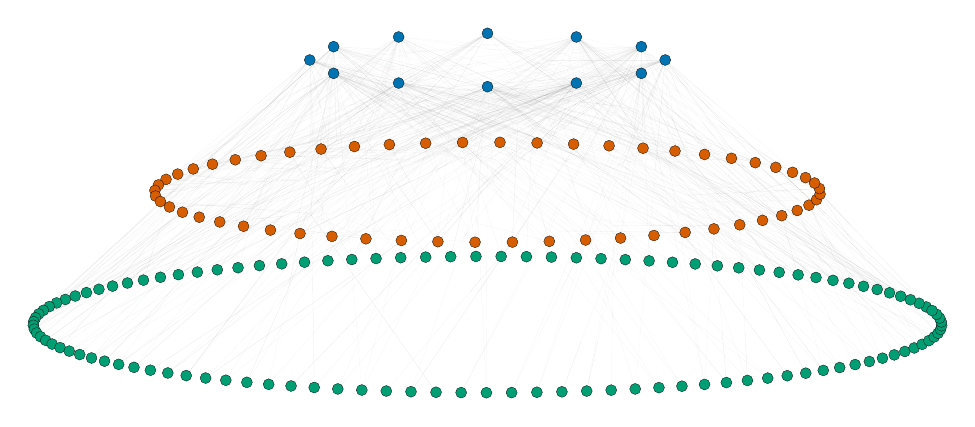
\begin{tikzpicture}[scale=1.4]
  \draw[gray, line width=0.08pt, opacity=0.10] (1.612,1.200) -- (1.272,1.310);
  \draw[gray, line width=0.08pt, opacity=0.10] (0.806,1.409) -- (1.272,1.310);
  \draw[gray, line width=0.08pt, opacity=0.10] (1.396,1.321) -- (1.272,1.310);
  \draw[gray, line width=0.08pt, opacity=0.10] (1.612,1.200) -- (1.731,0.914);
  \draw[gray, line width=0.08pt, opacity=0.10] (1.969,0.343) -- (1.731,0.914);
  \draw[gray, line width=0.08pt, opacity=0.10] (1.612,1.200) -- (1.731,0.914);
  \draw[gray, line width=0.08pt, opacity=0.10] (1.612,1.200) -- (0.529,0.876);
  \draw[gray, line width=0.08pt, opacity=0.10] (0.781,0.437) -- (0.529,0.876);
  \draw[gray, line width=0.08pt, opacity=0.10] (-0.806,0.991) -- (0.529,0.876);
  \draw[gray, line width=0.08pt, opacity=0.10] (1.612,1.200) -- (0.113,0.830);
  \draw[gray, line width=0.08pt, opacity=0.10] (-2.669,0.212) -- (0.113,0.830);
  \draw[gray, line width=0.08pt, opacity=0.10] (1.396,1.079) -- (0.113,0.830);
  \draw[gray, line width=0.08pt, opacity=0.10] (1.612,1.200) -- (-1.704,0.109);
  \draw[gray, line width=0.08pt, opacity=0.10] (-2.985,0.067) -- (-1.704,0.109);
  \draw[gray, line width=0.08pt, opacity=0.10] (-3.740,-0.941) -- (-1.704,0.109);
  \draw[gray, line width=0.08pt, opacity=0.10] (1.612,1.200) -- (0.983,-0.349);
  \draw[gray, line width=0.08pt, opacity=0.10] (0.890,-0.433) -- (0.983,-0.349);
  \draw[gray, line width=0.08pt, opacity=0.10] (0.448,-1.814) -- (0.983,-0.349);
  \draw[gray, line width=0.08pt, opacity=0.10] (1.612,1.200) -- (2.081,0.794);
  \draw[gray, line width=0.08pt, opacity=0.10] (3.017,-0.017) -- (2.081,0.794);
  \draw[gray, line width=0.08pt, opacity=0.10] (1.612,1.200) -- (2.081,0.794);
  \draw[gray, line width=0.08pt, opacity=0.10] (1.612,1.200) -- (2.331,0.230);
  \draw[gray, line width=0.08pt, opacity=0.10] (3.411,-0.853) -- (2.331,0.230);
  \draw[gray, line width=0.08pt, opacity=0.10] (1.969,0.343) -- (2.331,0.230);
  \draw[gray, line width=0.08pt, opacity=0.10] (1.612,1.200) -- (-0.700,0.299);
  \draw[gray, line width=0.08pt, opacity=0.10] (-1.660,-0.634) -- (-0.700,0.299);
  \draw[gray, line width=0.08pt, opacity=0.10] (-2.054,0.332) -- (-0.700,0.299);
  \draw[gray, line width=0.08pt, opacity=0.10] (1.612,1.200) -- (-0.440,0.417);
  \draw[gray, line width=0.08pt, opacity=0.10] (-3.740,-0.941) -- (-0.440,0.417);
  \draw[gray, line width=0.08pt, opacity=0.10] (0.806,0.991) -- (-0.440,0.417);
  \draw[gray, line width=0.08pt, opacity=0.10] (1.612,1.200) -- (1.522,0.205);
  \draw[gray, line width=0.08pt, opacity=0.10] (1.340,-1.784) -- (1.522,0.205);
  \draw[gray, line width=0.08pt, opacity=0.10] (1.612,1.200) -- (1.522,0.205);
  \draw[gray, line width=0.08pt, opacity=0.10] (1.612,1.200) -- (1.314,0.340);
  \draw[gray, line width=0.08pt, opacity=0.10] (3.943,-1.379) -- (1.314,0.340);
  \draw[gray, line width=0.08pt, opacity=0.10] (-1.612,1.200) -- (1.314,0.340);
  \draw[gray, line width=0.08pt, opacity=0.10] (1.396,1.321) -- (0.465,1.240);
  \draw[gray, line width=0.08pt, opacity=0.10] (0.806,0.991) -- (0.465,1.240);
  \draw[gray, line width=0.08pt, opacity=0.10] (-0.806,1.409) -- (0.465,1.240);
  \draw[gray, line width=0.08pt, opacity=0.10] (1.396,1.321) -- (0.936,1.054);
  \draw[gray, line width=0.08pt, opacity=0.10] (1.411,0.400) -- (0.936,1.054);
  \draw[gray, line width=0.08pt, opacity=0.10] (0.000,1.442) -- (0.936,1.054);
  \draw[gray, line width=0.08pt, opacity=0.10] (1.396,1.321) -- (0.765,0.739);
  \draw[gray, line width=0.08pt, opacity=0.10] (0.450,0.448) -- (0.765,0.739);
  \draw[gray, line width=0.08pt, opacity=0.10] (0.450,0.448) -- (0.765,0.739);
  \draw[gray, line width=0.08pt, opacity=0.10] (1.396,1.321) -- (-0.306,1.041);
  \draw[gray, line width=0.08pt, opacity=0.10] (-1.510,0.392) -- (-0.306,1.041);
  \draw[gray, line width=0.08pt, opacity=0.10] (-0.806,1.409) -- (-0.306,1.041);
  \draw[gray, line width=0.08pt, opacity=0.10] (1.396,1.321) -- (-0.219,0.870);
  \draw[gray, line width=0.08pt, opacity=0.10] (-2.054,0.332) -- (-0.219,0.870);
  \draw[gray, line width=0.08pt, opacity=0.10] (-0.000,0.958) -- (-0.219,0.870);
  \draw[gray, line width=0.08pt, opacity=0.10] (1.396,1.321) -- (0.272,0.620);
  \draw[gray, line width=0.08pt, opacity=0.10] (0.226,-0.452) -- (0.272,0.620);
  \draw[gray, line width=0.08pt, opacity=0.10] (-0.806,0.991) -- (0.272,0.620);
  \draw[gray, line width=0.08pt, opacity=0.10] (1.396,1.321) -- (1.950,0.466);
  \draw[gray, line width=0.08pt, opacity=0.10] (3.647,-0.912) -- (1.950,0.466);
  \draw[gray, line width=0.08pt, opacity=0.10] (0.806,0.991) -- (1.950,0.466);
  \draw[gray, line width=0.08pt, opacity=0.10] (1.396,1.321) -- (1.420,0.673);
  \draw[gray, line width=0.08pt, opacity=0.10] (1.466,-0.622) -- (1.420,0.673);
  \draw[gray, line width=0.08pt, opacity=0.10] (1.396,1.321) -- (1.420,0.673);
  \draw[gray, line width=0.08pt, opacity=0.10] (1.396,1.321) -- (0.668,0.683);
  \draw[gray, line width=0.08pt, opacity=0.10] (-0.787,-0.593) -- (0.668,0.683);
  \draw[gray, line width=0.08pt, opacity=0.10] (1.396,1.321) -- (0.668,0.683);
  \draw[gray, line width=0.08pt, opacity=0.10] (1.396,1.321) -- (-0.157,0.543);
  \draw[gray, line width=0.08pt, opacity=0.10] (-1.867,-0.649) -- (-0.157,0.543);
  \draw[gray, line width=0.08pt, opacity=0.10] (-0.000,0.958) -- (-0.157,0.543);
  \draw[gray, line width=0.08pt, opacity=0.10] (1.396,1.321) -- (0.851,0.275);
  \draw[gray, line width=0.08pt, opacity=0.10] (-0.239,-1.817) -- (0.851,0.275);
  \draw[gray, line width=0.08pt, opacity=0.10] (1.396,1.321) -- (0.851,0.275);
  \draw[gray, line width=0.08pt, opacity=0.10] (0.806,1.409) -- (0.269,1.270);
  \draw[gray, line width=0.08pt, opacity=0.10] (-1.396,1.079) -- (0.269,1.270);
  \draw[gray, line width=0.08pt, opacity=0.10] (1.396,1.321) -- (0.269,1.270);
  \draw[gray, line width=0.08pt, opacity=0.10] (0.806,1.409) -- (1.880,0.328);
  \draw[gray, line width=0.08pt, opacity=0.10] (1.701,0.374) -- (1.880,0.328);
  \draw[gray, line width=0.08pt, opacity=0.10] (3.134,-0.799) -- (1.880,0.328);
  \draw[gray, line width=0.08pt, opacity=0.10] (0.806,1.409) -- (-0.599,1.048);
  \draw[gray, line width=0.08pt, opacity=0.10] (-1.207,0.415) -- (-0.599,1.048);
  \draw[gray, line width=0.08pt, opacity=0.10] (-1.396,1.321) -- (-0.599,1.048);
  \draw[gray, line width=0.08pt, opacity=0.10] (0.806,1.409) -- (-0.739,0.388);
  \draw[gray, line width=0.08pt, opacity=0.10] (-1.793,0.364) -- (-0.739,0.388);
  \draw[gray, line width=0.08pt, opacity=0.10] (-1.231,-0.610) -- (-0.739,0.388);
  \draw[gray, line width=0.08pt, opacity=0.10] (0.806,1.409) -- (0.067,0.806);
  \draw[gray, line width=0.08pt, opacity=0.10] (-1.411,-0.400) -- (0.067,0.806);
  \draw[gray, line width=0.08pt, opacity=0.10] (0.806,1.409) -- (0.067,0.806);
  \draw[gray, line width=0.08pt, opacity=0.10] (0.806,1.409) -- (1.427,0.869);
  \draw[gray, line width=0.08pt, opacity=0.10] (2.669,-0.212) -- (1.427,0.869);
  \draw[gray, line width=0.08pt, opacity=0.10] (0.806,1.409) -- (1.427,0.869);
  \draw[gray, line width=0.08pt, opacity=0.10] (0.806,1.409) -- (1.543,0.934);
  \draw[gray, line width=0.08pt, opacity=0.10] (3.017,-0.017) -- (1.543,0.934);
  \draw[gray, line width=0.08pt, opacity=0.10] (0.806,1.409) -- (1.543,0.934);
  \draw[gray, line width=0.08pt, opacity=0.10] (0.806,1.409) -- (1.313,0.684);
  \draw[gray, line width=0.08pt, opacity=0.10] (3.134,-0.799) -- (1.313,0.684);
  \draw[gray, line width=0.08pt, opacity=0.10] (0.000,1.442) -- (1.313,0.684);
  \draw[gray, line width=0.08pt, opacity=0.10] (0.806,1.409) -- (1.360,0.565);
  \draw[gray, line width=0.08pt, opacity=0.10] (2.467,-0.705) -- (1.360,0.565);
  \draw[gray, line width=0.08pt, opacity=0.10] (0.806,0.991) -- (1.360,0.565);
  \draw[gray, line width=0.08pt, opacity=0.10] (0.806,1.409) -- (-0.142,0.586);
  \draw[gray, line width=0.08pt, opacity=0.10] (-1.231,-0.610) -- (-0.142,0.586);
  \draw[gray, line width=0.08pt, opacity=0.10] (-0.000,0.958) -- (-0.142,0.586);
  \draw[gray, line width=0.08pt, opacity=0.10] (0.806,1.409) -- (-0.233,0.364);
  \draw[gray, line width=0.08pt, opacity=0.10] (-2.900,-1.639) -- (-0.233,0.364);
  \draw[gray, line width=0.08pt, opacity=0.10] (1.396,1.321) -- (-0.233,0.364);
  \draw[gray, line width=0.08pt, opacity=0.10] (0.806,1.409) -- (1.284,0.250);
  \draw[gray, line width=0.08pt, opacity=0.10] (3.046,-1.616) -- (1.284,0.250);
  \draw[gray, line width=0.08pt, opacity=0.10] (-0.000,0.958) -- (1.284,0.250);
  \draw[gray, line width=0.08pt, opacity=0.10] (0.806,1.409) -- (1.895,0.571);
  \draw[gray, line width=0.08pt, opacity=0.10] (4.074,-1.107) -- (1.895,0.571);
  \draw[gray, line width=0.08pt, opacity=0.10] (0.806,1.409) -- (1.895,0.571);
  \draw[gray, line width=0.08pt, opacity=0.10] (0.000,1.442) -- (0.734,1.251);
  \draw[gray, line width=0.08pt, opacity=0.10] (0.806,0.991) -- (0.734,1.251);
  \draw[gray, line width=0.08pt, opacity=0.10] (1.396,1.321) -- (0.734,1.251);
  \draw[gray, line width=0.08pt, opacity=0.10] (0.000,1.442) -- (-0.832,1.046);
  \draw[gray, line width=0.08pt, opacity=0.10] (-2.495,0.255) -- (-0.832,1.046);
  \draw[gray, line width=0.08pt, opacity=0.10] (0.000,1.442) -- (-0.832,1.046);
  \draw[gray, line width=0.08pt, opacity=0.10] (0.000,1.442) -- (-1.879,0.294);
  \draw[gray, line width=0.08pt, opacity=0.10] (-2.669,0.212) -- (-1.879,0.294);
  \draw[gray, line width=0.08pt, opacity=0.10] (-2.967,-0.771) -- (-1.879,0.294);
  \draw[gray, line width=0.08pt, opacity=0.10] (0.000,1.442) -- (-1.122,0.807);
  \draw[gray, line width=0.08pt, opacity=0.10] (-1.969,-0.343) -- (-1.122,0.807);
  \draw[gray, line width=0.08pt, opacity=0.10] (-1.396,1.321) -- (-1.122,0.807);
  \draw[gray, line width=0.08pt, opacity=0.10] (0.000,1.442) -- (-1.636,-0.173);
  \draw[gray, line width=0.08pt, opacity=0.10] (-1.701,-0.374) -- (-1.636,-0.173);
  \draw[gray, line width=0.08pt, opacity=0.10] (-3.207,-1.588) -- (-1.636,-0.173);
  \draw[gray, line width=0.08pt, opacity=0.10] (0.000,1.442) -- (1.262,0.553);
  \draw[gray, line width=0.08pt, opacity=0.10] (2.980,-0.773) -- (1.262,0.553);
  \draw[gray, line width=0.08pt, opacity=0.10] (0.806,0.991) -- (1.262,0.553);
  \draw[gray, line width=0.08pt, opacity=0.10] (0.000,1.442) -- (-0.524,0.583);
  \draw[gray, line width=0.08pt, opacity=0.10] (-2.967,-0.771) -- (-0.524,0.583);
  \draw[gray, line width=0.08pt, opacity=0.10] (1.396,1.079) -- (-0.524,0.583);
  \draw[gray, line width=0.08pt, opacity=0.10] (0.000,1.442) -- (-1.624,0.410);
  \draw[gray, line width=0.08pt, opacity=0.10] (-3.474,-1.532) -- (-1.624,0.410);
  \draw[gray, line width=0.08pt, opacity=0.10] (-1.396,1.321) -- (-1.624,0.410);
  \draw[gray, line width=0.08pt, opacity=0.10] (0.000,1.442) -- (1.372,0.569);
  \draw[gray, line width=0.08pt, opacity=0.10] (4.117,-1.176) -- (1.372,0.569);
  \draw[gray, line width=0.08pt, opacity=0.10] (0.000,1.442) -- (1.372,0.569);
  \draw[gray, line width=0.08pt, opacity=0.10] (-0.806,1.409) -- (-0.734,1.230);
  \draw[gray, line width=0.08pt, opacity=0.10] (-1.396,1.321) -- (-0.734,1.230);
  \draw[gray, line width=0.08pt, opacity=0.10] (-0.000,0.958) -- (-0.734,1.230);
  \draw[gray, line width=0.08pt, opacity=0.10] (-0.806,1.409) -- (-0.306,0.960);
  \draw[gray, line width=0.08pt, opacity=0.10] (-1.510,0.392) -- (-0.306,0.960);
  \draw[gray, line width=0.08pt, opacity=0.10] (1.396,1.079) -- (-0.306,0.960);
  \draw[gray, line width=0.08pt, opacity=0.10] (-0.806,1.409) -- (-2.259,0.515);
  \draw[gray, line width=0.08pt, opacity=0.10] (-2.985,0.067) -- (-2.259,0.515);
  \draw[gray, line width=0.08pt, opacity=0.10] (-2.985,0.067) -- (-2.259,0.515);
  \draw[gray, line width=0.08pt, opacity=0.10] (-0.806,1.409) -- (-1.391,0.796);
  \draw[gray, line width=0.08pt, opacity=0.10] (-1.969,-0.343) -- (-1.391,0.796);
  \draw[gray, line width=0.08pt, opacity=0.10] (-1.396,1.321) -- (-1.391,0.796);
  \draw[gray, line width=0.08pt, opacity=0.10] (-0.806,1.409) -- (-1.547,-0.225);
  \draw[gray, line width=0.08pt, opacity=0.10] (-1.103,-0.422) -- (-1.547,-0.225);
  \draw[gray, line width=0.08pt, opacity=0.10] (-2.733,-1.663) -- (-1.547,-0.225);
  \draw[gray, line width=0.08pt, opacity=0.10] (-0.806,1.409) -- (-0.038,0.649);
  \draw[gray, line width=0.08pt, opacity=0.10] (-0.113,-0.453) -- (-0.038,0.649);
  \draw[gray, line width=0.08pt, opacity=0.10] (0.806,0.991) -- (-0.038,0.649);
  \draw[gray, line width=0.08pt, opacity=0.10] (-0.806,1.409) -- (1.169,0.790);
  \draw[gray, line width=0.08pt, opacity=0.10] (2.916,-0.117) -- (1.169,0.790);
  \draw[gray, line width=0.08pt, opacity=0.10] (1.396,1.079) -- (1.169,0.790);
  \draw[gray, line width=0.08pt, opacity=0.10] (-0.806,1.409) -- (-1.071,0.629);
  \draw[gray, line width=0.08pt, opacity=0.10] (-1.011,-0.601) -- (-1.071,0.629);
  \draw[gray, line width=0.08pt, opacity=0.10] (-1.396,1.079) -- (-1.071,0.629);
  \draw[gray, line width=0.08pt, opacity=0.10] (-0.806,1.409) -- (-2.477,0.189);
  \draw[gray, line width=0.08pt, opacity=0.10] (-3.638,-0.910) -- (-2.477,0.189);
  \draw[gray, line width=0.08pt, opacity=0.10] (-2.985,0.067) -- (-2.477,0.189);
  \draw[gray, line width=0.08pt, opacity=0.10] (-0.806,1.409) -- (-2.123,-0.146);
  \draw[gray, line width=0.08pt, opacity=0.10] (-3.592,-1.503) -- (-2.123,-0.146);
  \draw[gray, line width=0.08pt, opacity=0.10] (-1.969,-0.343) -- (-2.123,-0.146);
  \draw[gray, line width=0.08pt, opacity=0.10] (-0.806,1.409) -- (-1.257,-0.251);
  \draw[gray, line width=0.08pt, opacity=0.10] (-2.183,-1.724) -- (-1.257,-0.251);
  \draw[gray, line width=0.08pt, opacity=0.10] (-0.781,-0.437) -- (-1.257,-0.251);
  \draw[gray, line width=0.08pt, opacity=0.10] (-0.806,1.409) -- (1.686,-0.131);
  \draw[gray, line width=0.08pt, opacity=0.10] (3.195,-1.590) -- (1.686,-0.131);
  \draw[gray, line width=0.08pt, opacity=0.10] (2.669,-0.212) -- (1.686,-0.131);
  \draw[gray, line width=0.08pt, opacity=0.10] (-1.396,1.321) -- (-0.662,1.270);
  \draw[gray, line width=0.08pt, opacity=0.10] (0.806,1.409) -- (-0.662,1.270);
  \draw[gray, line width=0.08pt, opacity=0.10] (-1.396,1.079) -- (-0.662,1.270);
  \draw[gray, line width=0.08pt, opacity=0.10] (-1.396,1.321) -- (-0.059,0.956);
  \draw[gray, line width=0.08pt, opacity=0.10] (2.615,0.226) -- (-0.059,0.956);
  \draw[gray, line width=0.08pt, opacity=0.10] (-1.396,1.321) -- (-0.059,0.956);
  \draw[gray, line width=0.08pt, opacity=0.10] (-1.396,1.321) -- (-1.738,0.899);
  \draw[gray, line width=0.08pt, opacity=0.10] (-3.011,-0.034) -- (-1.738,0.899);
  \draw[gray, line width=0.08pt, opacity=0.10] (-0.806,1.409) -- (-1.738,0.899);
  \draw[gray, line width=0.08pt, opacity=0.10] (-1.396,1.321) -- (-2.443,0.384);
  \draw[gray, line width=0.08pt, opacity=0.10] (-2.967,-0.084) -- (-2.443,0.384);
  \draw[gray, line width=0.08pt, opacity=0.10] (-2.967,-0.084) -- (-2.443,0.384);
  \draw[gray, line width=0.08pt, opacity=0.10] (-1.396,1.321) -- (-1.941,0.235);
  \draw[gray, line width=0.08pt, opacity=0.10] (-2.213,-0.308) -- (-1.941,0.235);
  \draw[gray, line width=0.08pt, opacity=0.10] (-2.213,-0.308) -- (-1.941,0.235);
  \draw[gray, line width=0.08pt, opacity=0.10] (-1.396,1.321) -- (0.187,0.732);
  \draw[gray, line width=0.08pt, opacity=0.10] (0.561,-0.445) -- (0.187,0.732);
  \draw[gray, line width=0.08pt, opacity=0.10] (1.396,1.321) -- (0.187,0.732);
  \draw[gray, line width=0.08pt, opacity=0.10] (-1.396,1.321) -- (0.941,-0.246);
  \draw[gray, line width=0.08pt, opacity=0.10] (2.054,-0.332) -- (0.941,-0.246);
  \draw[gray, line width=0.08pt, opacity=0.10] (2.167,-1.726) -- (0.941,-0.246);
  \draw[gray, line width=0.08pt, opacity=0.10] (-1.396,1.321) -- (0.593,0.424);
  \draw[gray, line width=0.08pt, opacity=0.10] (3.980,-1.040) -- (0.593,0.424);
  \draw[gray, line width=0.08pt, opacity=0.10] (-0.806,0.991) -- (0.593,0.424);
  \draw[gray, line width=0.08pt, opacity=0.10] (-1.396,1.321) -- (-1.370,0.467);
  \draw[gray, line width=0.08pt, opacity=0.10] (-4.111,-1.241) -- (-1.370,0.467);
  \draw[gray, line width=0.08pt, opacity=0.10] (1.396,1.321) -- (-1.370,0.467);
  \draw[gray, line width=0.08pt, opacity=0.10] (-1.396,1.321) -- (-1.311,0.283);
  \draw[gray, line width=0.08pt, opacity=0.10] (-1.140,-1.794) -- (-1.311,0.283);
  \draw[gray, line width=0.08pt, opacity=0.10] (-1.396,1.321) -- (-1.311,0.283);
  \draw[gray, line width=0.08pt, opacity=0.10] (-1.396,1.321) -- (-0.003,0.275);
  \draw[gray, line width=0.08pt, opacity=0.10] (-0.010,-1.818) -- (-0.003,0.275);
  \draw[gray, line width=0.08pt, opacity=0.10] (1.396,1.321) -- (-0.003,0.275);
  \draw[gray, line width=0.08pt, opacity=0.10] (-1.396,1.321) -- (-0.083,0.318);
  \draw[gray, line width=0.08pt, opacity=0.10] (2.542,-1.686) -- (-0.083,0.318);
  \draw[gray, line width=0.08pt, opacity=0.10] (-1.396,1.321) -- (-0.083,0.318);
  \draw[gray, line width=0.08pt, opacity=0.10] (-1.612,1.200) -- (-0.537,1.281);
  \draw[gray, line width=0.08pt, opacity=0.10] (-1.396,1.321) -- (-0.537,1.281);
  \draw[gray, line width=0.08pt, opacity=0.10] (1.396,1.321) -- (-0.537,1.281);
  \draw[gray, line width=0.08pt, opacity=0.10] (-1.612,1.200) -- (0.119,0.834);
  \draw[gray, line width=0.08pt, opacity=0.10] (1.969,0.343) -- (0.119,0.834);
  \draw[gray, line width=0.08pt, opacity=0.10] (-0.000,0.958) -- (0.119,0.834);
  \draw[gray, line width=0.08pt, opacity=0.10] (-1.612,1.200) -- (-1.510,0.758);
  \draw[gray, line width=0.08pt, opacity=0.10] (-2.916,0.117) -- (-1.510,0.758);
  \draw[gray, line width=0.08pt, opacity=0.10] (-0.000,0.958) -- (-1.510,0.758);
  \draw[gray, line width=0.08pt, opacity=0.10] (-1.612,1.200) -- (-1.078,0.765);
  \draw[gray, line width=0.08pt, opacity=0.10] (-3.017,0.017) -- (-1.078,0.765);
  \draw[gray, line width=0.08pt, opacity=0.10] (1.396,1.079) -- (-1.078,0.765);
  \draw[gray, line width=0.08pt, opacity=0.10] (-1.612,1.200) -- (-0.882,0.751);
  \draw[gray, line width=0.08pt, opacity=0.10] (-2.429,-0.269) -- (-0.882,0.751);
  \draw[gray, line width=0.08pt, opacity=0.10] (1.396,1.321) -- (-0.882,0.751);
  \draw[gray, line width=0.08pt, opacity=0.10] (-1.612,1.200) -- (-0.837,0.101);
  \draw[gray, line width=0.08pt, opacity=0.10] (-0.450,-0.448) -- (-0.837,0.101);
  \draw[gray, line width=0.08pt, opacity=0.10] (-0.450,-0.448) -- (-0.837,0.101);
  \draw[gray, line width=0.08pt, opacity=0.10] (-1.612,1.200) -- (1.817,-0.026);
  \draw[gray, line width=0.08pt, opacity=0.10] (3.011,0.034) -- (1.817,-0.026);
  \draw[gray, line width=0.08pt, opacity=0.10] (4.052,-1.312) -- (1.817,-0.026);
  \draw[gray, line width=0.08pt, opacity=0.10] (-1.612,1.200) -- (0.555,0.444);
  \draw[gray, line width=0.08pt, opacity=0.10] (3.278,-0.825) -- (0.555,0.444);
  \draw[gray, line width=0.08pt, opacity=0.10] (-0.000,0.958) -- (0.555,0.444);
  \draw[gray, line width=0.08pt, opacity=0.10] (-1.612,1.200) -- (-2.684,0.146);
  \draw[gray, line width=0.08pt, opacity=0.10] (-3.525,-0.880) -- (-2.684,0.146);
  \draw[gray, line width=0.08pt, opacity=0.10] (-2.916,0.117) -- (-2.684,0.146);
  \draw[gray, line width=0.08pt, opacity=0.10] (-1.612,1.200) -- (-1.435,0.415);
  \draw[gray, line width=0.08pt, opacity=0.10] (-4.090,-1.276) -- (-1.435,0.415);
  \draw[gray, line width=0.08pt, opacity=0.10] (1.396,1.321) -- (-1.435,0.415);
  \draw[gray, line width=0.08pt, opacity=0.10] (-1.612,1.200) -- (-1.561,0.260);
  \draw[gray, line width=0.08pt, opacity=0.10] (-3.877,-1.409) -- (-1.561,0.260);
  \draw[gray, line width=0.08pt, opacity=0.10] (0.806,0.991) -- (-1.561,0.260);
  \draw[gray, line width=0.08pt, opacity=0.10] (-1.612,1.200) -- (0.276,0.363);
  \draw[gray, line width=0.08pt, opacity=0.10] (4.052,-1.312) -- (0.276,0.363);
  \draw[gray, line width=0.08pt, opacity=0.10] (-1.612,1.200) -- (0.276,0.363);
  \draw[gray, line width=0.08pt, opacity=0.10] (-1.396,1.079) -- (0.269,1.189);
  \draw[gray, line width=0.08pt, opacity=0.10] (0.806,1.409) -- (0.269,1.189);
  \draw[gray, line width=0.08pt, opacity=0.10] (1.396,1.079) -- (0.269,1.189);
  \draw[gray, line width=0.08pt, opacity=0.10] (-1.396,1.079) -- (-0.893,0.870);
  \draw[gray, line width=0.08pt, opacity=0.10] (0.113,0.453) -- (-0.893,0.870);
  \draw[gray, line width=0.08pt, opacity=0.10] (-1.396,1.079) -- (-0.893,0.870);
  \draw[gray, line width=0.08pt, opacity=0.10] (-1.396,1.079) -- (-0.794,0.951);
  \draw[gray, line width=0.08pt, opacity=0.10] (-1.793,0.364) -- (-0.794,0.951);
  \draw[gray, line width=0.08pt, opacity=0.10] (0.806,1.409) -- (-0.794,0.951);
  \draw[gray, line width=0.08pt, opacity=0.10] (-1.396,1.079) -- (-0.934,0.765);
  \draw[gray, line width=0.08pt, opacity=0.10] (-3.017,0.017) -- (-0.934,0.765);
  \draw[gray, line width=0.08pt, opacity=0.10] (1.612,1.200) -- (-0.934,0.765);
  \draw[gray, line width=0.08pt, opacity=0.10] (-1.396,1.079) -- (-1.669,0.697);
  \draw[gray, line width=0.08pt, opacity=0.10] (-2.213,-0.308) -- (-1.669,0.697);
  \draw[gray, line width=0.08pt, opacity=0.10] (-1.396,1.321) -- (-1.669,0.697);
  \draw[gray, line width=0.08pt, opacity=0.10] (-1.396,1.079) -- (-0.567,0.595);
  \draw[gray, line width=0.08pt, opacity=0.10] (-1.701,-0.374) -- (-0.567,0.595);
  \draw[gray, line width=0.08pt, opacity=0.10] (1.396,1.079) -- (-0.567,0.595);
  \draw[gray, line width=0.08pt, opacity=0.10] (-1.396,1.079) -- (0.650,-0.353);
  \draw[gray, line width=0.08pt, opacity=0.10] (1.793,-0.364) -- (0.650,-0.353);
  \draw[gray, line width=0.08pt, opacity=0.10] (1.555,-1.772) -- (0.650,-0.353);
  \draw[gray, line width=0.08pt, opacity=0.10] (-1.396,1.079) -- (-0.039,0.565);
  \draw[gray, line width=0.08pt, opacity=0.10] (-0.334,-0.584) -- (-0.039,0.565);
  \draw[gray, line width=0.08pt, opacity=0.10] (1.612,1.200) -- (-0.039,0.565);
  \draw[gray, line width=0.08pt, opacity=0.10] (-1.396,1.079) -- (-1.546,0.274);
  \draw[gray, line width=0.08pt, opacity=0.10] (-1.448,-0.621) -- (-1.546,0.274);
  \draw[gray, line width=0.08pt, opacity=0.10] (-1.793,0.364) -- (-1.546,0.274);
  \draw[gray, line width=0.08pt, opacity=0.10] (-1.396,1.079) -- (-1.500,0.355);
  \draw[gray, line width=0.08pt, opacity=0.10] (-3.909,-1.004) -- (-1.500,0.355);
  \draw[gray, line width=0.08pt, opacity=0.10] (0.806,0.991) -- (-1.500,0.355);
  \draw[gray, line width=0.08pt, opacity=0.10] (-1.396,1.079) -- (-2.046,0.280);
  \draw[gray, line width=0.08pt, opacity=0.10] (-3.346,-1.561) -- (-2.046,0.280);
  \draw[gray, line width=0.08pt, opacity=0.10] (-1.396,1.321) -- (-2.046,0.280);
  \draw[gray, line width=0.08pt, opacity=0.10] (-1.396,1.079) -- (1.227,0.248);
  \draw[gray, line width=0.08pt, opacity=0.10] (3.464,-1.535) -- (1.227,0.248);
  \draw[gray, line width=0.08pt, opacity=0.10] (1.612,1.200) -- (1.227,0.248);
  \draw[gray, line width=0.08pt, opacity=0.10] (-0.806,0.991) -- (-0.537,1.119);
  \draw[gray, line width=0.08pt, opacity=0.10] (-0.806,1.409) -- (-0.537,1.119);
  \draw[gray, line width=0.08pt, opacity=0.10] (-0.000,0.958) -- (-0.537,1.119);
  \draw[gray, line width=0.08pt, opacity=0.10] (-0.806,0.991) -- (1.351,0.509);
  \draw[gray, line width=0.08pt, opacity=0.10] (2.429,0.269) -- (1.351,0.509);
  \draw[gray, line width=0.08pt, opacity=0.10] (2.429,0.269) -- (1.351,0.509);
  \draw[gray, line width=0.08pt, opacity=0.10] (-0.806,0.991) -- (0.194,0.881);
  \draw[gray, line width=0.08pt, opacity=0.10] (-0.226,0.452) -- (0.194,0.881);
  \draw[gray, line width=0.08pt, opacity=0.10] (1.612,1.200) -- (0.194,0.881);
  \draw[gray, line width=0.08pt, opacity=0.10] (-0.806,0.991) -- (-2.294,0.111);
  \draw[gray, line width=0.08pt, opacity=0.10] (-2.810,0.165) -- (-2.294,0.111);
  \draw[gray, line width=0.08pt, opacity=0.10] (-3.266,-0.823) -- (-2.294,0.111);
  \draw[gray, line width=0.08pt, opacity=0.10] (-0.806,0.991) -- (-1.606,0.614);
  \draw[gray, line width=0.08pt, opacity=0.10] (-2.615,-0.226) -- (-1.606,0.614);
  \draw[gray, line width=0.08pt, opacity=0.10] (-1.396,1.079) -- (-1.606,0.614);
  \draw[gray, line width=0.08pt, opacity=0.10] (-0.806,0.991) -- (1.200,0.782);
  \draw[gray, line width=0.08pt, opacity=0.10] (3.011,0.034) -- (1.200,0.782);
  \draw[gray, line width=0.08pt, opacity=0.10] (1.396,1.321) -- (1.200,0.782);
  \draw[gray, line width=0.08pt, opacity=0.10] (-0.806,0.991) -- (1.998,0.033);
  \draw[gray, line width=0.08pt, opacity=0.10] (2.767,0.181) -- (1.998,0.033);
  \draw[gray, line width=0.08pt, opacity=0.10] (4.033,-1.073) -- (1.998,0.033);
  \draw[gray, line width=0.08pt, opacity=0.10] (-0.806,0.991) -- (0.670,0.400);
  \draw[gray, line width=0.08pt, opacity=0.10] (2.818,-0.749) -- (0.670,0.400);
  \draw[gray, line width=0.08pt, opacity=0.10] (-0.000,0.958) -- (0.670,0.400);
  \draw[gray, line width=0.08pt, opacity=0.10] (-0.806,0.991) -- (-2.294,0.111);
  \draw[gray, line width=0.08pt, opacity=0.10] (-3.266,-0.823) -- (-2.294,0.111);
  \draw[gray, line width=0.08pt, opacity=0.10] (-2.810,0.165) -- (-2.294,0.111);
  \draw[gray, line width=0.08pt, opacity=0.10] (-0.806,0.991) -- (-1.874,0.213);
  \draw[gray, line width=0.08pt, opacity=0.10] (-4.008,-1.343) -- (-1.874,0.213);
  \draw[gray, line width=0.08pt, opacity=0.10] (-0.806,0.991) -- (-1.874,0.213);
  \draw[gray, line width=0.08pt, opacity=0.10] (-0.806,0.991) -- (0.825,0.234);
  \draw[gray, line width=0.08pt, opacity=0.10] (4.087,-1.279) -- (0.825,0.234);
  \draw[gray, line width=0.08pt, opacity=0.10] (-0.806,0.991) -- (0.825,0.234);
  \draw[gray, line width=0.08pt, opacity=0.10] (-0.000,0.958) -- (0.537,1.200);
  \draw[gray, line width=0.08pt, opacity=0.10] (0.000,1.442) -- (0.537,1.200);
  \draw[gray, line width=0.08pt, opacity=0.10] (1.612,1.200) -- (0.537,1.200);
  \draw[gray, line width=0.08pt, opacity=0.10] (-0.000,0.958) -- (0.406,0.835);
  \draw[gray, line width=0.08pt, opacity=0.10] (2.615,0.226) -- (0.406,0.835);
  \draw[gray, line width=0.08pt, opacity=0.10] (-1.396,1.321) -- (0.406,0.835);
  \draw[gray, line width=0.08pt, opacity=0.10] (-0.000,0.958) -- (0.726,0.906);
  \draw[gray, line width=0.08pt, opacity=0.10] (0.781,0.437) -- (0.726,0.906);
  \draw[gray, line width=0.08pt, opacity=0.10] (1.396,1.321) -- (0.726,0.906);
  \draw[gray, line width=0.08pt, opacity=0.10] (-0.000,0.958) -- (0.278,0.827);
  \draw[gray, line width=0.08pt, opacity=0.10] (-0.561,0.445) -- (0.278,0.827);
  \draw[gray, line width=0.08pt, opacity=0.10] (1.396,1.079) -- (0.278,0.827);
  \draw[gray, line width=0.08pt, opacity=0.10] (-0.000,0.958) -- (-0.134,0.788);
  \draw[gray, line width=0.08pt, opacity=0.10] (-1.207,0.415) -- (-0.134,0.788);
  \draw[gray, line width=0.08pt, opacity=0.10] (0.806,0.991) -- (-0.134,0.788);
  \draw[gray, line width=0.08pt, opacity=0.10] (-0.000,0.958) -- (-0.906,0.588);
  \draw[gray, line width=0.08pt, opacity=0.10] (-1.510,0.392) -- (-0.906,0.588);
  \draw[gray, line width=0.08pt, opacity=0.10] (-1.207,0.415) -- (-0.906,0.588);
  \draw[gray, line width=0.08pt, opacity=0.10] (-0.000,0.958) -- (-0.668,0.705);
  \draw[gray, line width=0.08pt, opacity=0.10] (-2.810,0.165) -- (-0.668,0.705);
  \draw[gray, line width=0.08pt, opacity=0.10] (0.806,0.991) -- (-0.668,0.705);
  \draw[gray, line width=0.08pt, opacity=0.10] (-0.000,0.958) -- (1.100,0.565);
  \draw[gray, line width=0.08pt, opacity=0.10] (2.495,-0.255) -- (1.100,0.565);
  \draw[gray, line width=0.08pt, opacity=0.10] (0.806,0.991) -- (1.100,0.565);
  \draw[gray, line width=0.08pt, opacity=0.10] (-0.000,0.958) -- (0.767,0.384);
  \draw[gray, line width=0.08pt, opacity=0.10] (3.915,-1.007) -- (0.767,0.384);
  \draw[gray, line width=0.08pt, opacity=0.10] (-1.612,1.200) -- (0.767,0.384);
  \draw[gray, line width=0.08pt, opacity=0.10] (-0.000,0.958) -- (0.230,0.457);
  \draw[gray, line width=0.08pt, opacity=0.10] (2.085,-0.667) -- (0.230,0.457);
  \draw[gray, line width=0.08pt, opacity=0.10] (-1.396,1.079) -- (0.230,0.457);
  \draw[gray, line width=0.08pt, opacity=0.10] (-0.000,0.958) -- (-0.754,0.411);
  \draw[gray, line width=0.08pt, opacity=0.10] (-2.263,-0.684) -- (-0.754,0.411);
  \draw[gray, line width=0.08pt, opacity=0.10] (-0.000,0.958) -- (-0.754,0.411);
  \draw[gray, line width=0.08pt, opacity=0.10] (-0.000,0.958) -- (-1.134,0.355);
  \draw[gray, line width=0.08pt, opacity=0.10] (-3.401,-0.851) -- (-1.134,0.355);
  \draw[gray, line width=0.08pt, opacity=0.10] (-0.000,0.958) -- (-1.134,0.355);
  \draw[gray, line width=0.08pt, opacity=0.10] (-0.000,0.958) -- (2.329,-0.017);
  \draw[gray, line width=0.08pt, opacity=0.10] (4.102,-1.141) -- (2.329,-0.017);
  \draw[gray, line width=0.08pt, opacity=0.10] (2.885,0.133) -- (2.329,-0.017);
  \draw[gray, line width=0.08pt, opacity=0.10] (0.806,0.991) -- (0.269,1.130);
  \draw[gray, line width=0.08pt, opacity=0.10] (-0.806,0.991) -- (0.269,1.130);
  \draw[gray, line width=0.08pt, opacity=0.10] (0.806,1.409) -- (0.269,1.130);
  \draw[gray, line width=0.08pt, opacity=0.10] (0.806,0.991) -- (2.185,0.139);
  \draw[gray, line width=0.08pt, opacity=0.10] (2.213,0.308) -- (2.185,0.139);
  \draw[gray, line width=0.08pt, opacity=0.10] (3.535,-0.882) -- (2.185,0.139);
  \draw[gray, line width=0.08pt, opacity=0.10] (0.806,0.991) -- (-0.075,0.811);
  \draw[gray, line width=0.08pt, opacity=0.10] (-0.226,0.452) -- (-0.075,0.811);
  \draw[gray, line width=0.08pt, opacity=0.10] (-0.806,0.991) -- (-0.075,0.811);
  \draw[gray, line width=0.08pt, opacity=0.10] (0.806,0.991) -- (0.510,0.874);
  \draw[gray, line width=0.08pt, opacity=0.10] (-0.890,0.433) -- (0.510,0.874);
  \draw[gray, line width=0.08pt, opacity=0.10] (1.612,1.200) -- (0.510,0.874);
  \draw[gray, line width=0.08pt, opacity=0.10] (0.806,0.991) -- (-1.394,0.500);
  \draw[gray, line width=0.08pt, opacity=0.10] (-2.495,0.255) -- (-1.394,0.500);
  \draw[gray, line width=0.08pt, opacity=0.10] (-2.495,0.255) -- (-1.394,0.500);
  \draw[gray, line width=0.08pt, opacity=0.10] (0.806,0.991) -- (-0.031,0.032);
  \draw[gray, line width=0.08pt, opacity=0.10] (-0.450,-0.448) -- (-0.031,0.032);
  \draw[gray, line width=0.08pt, opacity=0.10] (-0.450,-0.448) -- (-0.031,0.032);
  \draw[gray, line width=0.08pt, opacity=0.10] (0.806,0.991) -- (1.912,0.476);
  \draw[gray, line width=0.08pt, opacity=0.10] (3.535,-0.882) -- (1.912,0.476);
  \draw[gray, line width=0.08pt, opacity=0.10] (1.396,1.321) -- (1.912,0.476);
  \draw[gray, line width=0.08pt, opacity=0.10] (0.806,0.991) -- (1.029,0.421);
  \draw[gray, line width=0.08pt, opacity=0.10] (2.279,-0.685) -- (1.029,0.421);
  \draw[gray, line width=0.08pt, opacity=0.10] (-0.000,0.958) -- (1.029,0.421);
  \draw[gray, line width=0.08pt, opacity=0.10] (0.806,0.991) -- (0.579,0.466);
  \draw[gray, line width=0.08pt, opacity=0.10] (0.124,-0.582) -- (0.579,0.466);
  \draw[gray, line width=0.08pt, opacity=0.10] (0.806,0.991) -- (0.579,0.466);
  \draw[gray, line width=0.08pt, opacity=0.10] (0.806,0.991) -- (-1.146,0.489);
  \draw[gray, line width=0.08pt, opacity=0.10] (-2.632,-0.724) -- (-1.146,0.489);
  \draw[gray, line width=0.08pt, opacity=0.10] (-1.612,1.200) -- (-1.146,0.489);
  \draw[gray, line width=0.08pt, opacity=0.10] (0.806,0.991) -- (-0.475,-0.405);
  \draw[gray, line width=0.08pt, opacity=0.10] (-1.782,-1.757) -- (-0.475,-0.405);
  \draw[gray, line width=0.08pt, opacity=0.10] (-0.450,-0.448) -- (-0.475,-0.405);
  \draw[gray, line width=0.08pt, opacity=0.10] (1.396,1.079) -- (0.465,1.299);
  \draw[gray, line width=0.08pt, opacity=0.10] (-0.806,1.409) -- (0.465,1.299);
  \draw[gray, line width=0.08pt, opacity=0.10] (0.806,1.409) -- (0.465,1.299);
  \draw[gray, line width=0.08pt, opacity=0.10] (1.396,1.079) -- (-0.031,0.756);
  \draw[gray, line width=0.08pt, opacity=0.10] (-2.885,-0.133) -- (-0.031,0.756);
  \draw[gray, line width=0.08pt, opacity=0.10] (1.396,1.321) -- (-0.031,0.756);
  \draw[gray, line width=0.08pt, opacity=0.10] (1.396,1.079) -- (-0.668,0.110);
  \draw[gray, line width=0.08pt, opacity=0.10] (-1.701,-0.374) -- (-0.668,0.110);
  \draw[gray, line width=0.08pt, opacity=0.10] (-1.701,-0.374) -- (-0.668,0.110);
  \draw[gray, line width=0.08pt, opacity=0.10] (1.396,1.079) -- (0.272,0.539);
  \draw[gray, line width=0.08pt, opacity=0.10] (0.226,-0.452) -- (0.272,0.539);
  \draw[gray, line width=0.08pt, opacity=0.10] (-0.806,0.991) -- (0.272,0.539);
  \draw[gray, line width=0.08pt, opacity=0.10] (1.396,1.079) -- (1.333,0.581);
  \draw[gray, line width=0.08pt, opacity=0.10] (1.207,-0.415) -- (1.333,0.581);
  \draw[gray, line width=0.08pt, opacity=0.10] (1.396,1.079) -- (1.333,0.581);
  \draw[gray, line width=0.08pt, opacity=0.10] (1.396,1.079) -- (1.297,0.594);
  \draw[gray, line width=0.08pt, opacity=0.10] (2.495,-0.255) -- (1.297,0.594);
  \draw[gray, line width=0.08pt, opacity=0.10] (-0.000,0.958) -- (1.297,0.594);
  \draw[gray, line width=0.08pt, opacity=0.10] (1.396,1.079) -- (1.745,0.354);
  \draw[gray, line width=0.08pt, opacity=0.10] (3.837,-0.975) -- (1.745,0.354);
  \draw[gray, line width=0.08pt, opacity=0.10] (-0.000,0.958) -- (1.745,0.354);
  \draw[gray, line width=0.08pt, opacity=0.10] (1.396,1.079) -- (-0.656,0.268);
  \draw[gray, line width=0.08pt, opacity=0.10] (-2.557,-1.685) -- (-0.656,0.268);
  \draw[gray, line width=0.08pt, opacity=0.10] (-0.806,1.409) -- (-0.656,0.268);
  \draw[gray, line width=0.08pt, opacity=0.10] (1.396,1.079) -- (-0.034,0.087);
  \draw[gray, line width=0.08pt, opacity=0.10] (-0.694,-1.809) -- (-0.034,0.087);
  \draw[gray, line width=0.08pt, opacity=0.10] (-0.806,0.991) -- (-0.034,0.087);
  \draw[gray, line width=0.08pt, opacity=0.10] (1.396,1.079) -- (1.659,0.179);
  \draw[gray, line width=0.08pt, opacity=0.10] (1.969,-1.743) -- (1.659,0.179);
  \draw[gray, line width=0.08pt, opacity=0.10] (1.612,1.200) -- (1.659,0.179);
  \draw[gray, line width=0.08pt, opacity=0.10] (1.396,1.079) -- (2.025,0.359);
  \draw[gray, line width=0.08pt, opacity=0.10] (3.871,-1.412) -- (2.025,0.359);
  \draw[gray, line width=0.08pt, opacity=0.10] (0.806,1.409) -- (2.025,0.359);
  \draw[gray, line width=0.08pt, opacity=0.10] (2.615,0.226) -- (0.675,0.846);
  \draw[gray, line width=0.08pt, opacity=0.10] (-1.396,1.321) -- (0.675,0.846);
  \draw[gray, line width=0.08pt, opacity=0.10] (0.806,0.991) -- (0.675,0.846);
  \draw[gray, line width=0.08pt, opacity=0.10] (2.615,0.226) -- (1.337,0.755);
  \draw[gray, line width=0.08pt, opacity=0.10] (-0.000,0.958) -- (1.337,0.755);
  \draw[gray, line width=0.08pt, opacity=0.10] (1.396,1.079) -- (1.337,0.755);
  \draw[gray, line width=0.08pt, opacity=0.10] (2.615,0.226) -- (3.070,-0.196);
  \draw[gray, line width=0.08pt, opacity=0.10] (3.980,-1.040) -- (3.070,-0.196);
  \draw[gray, line width=0.08pt, opacity=0.10] (2.615,0.226) -- (3.070,-0.196);
  \draw[gray, line width=0.08pt, opacity=0.10] (2.429,0.269) -- (0.541,0.739);
  \draw[gray, line width=0.08pt, opacity=0.10] (-0.806,0.991) -- (0.541,0.739);
  \draw[gray, line width=0.08pt, opacity=0.10] (-0.000,0.958) -- (0.541,0.739);
  \draw[gray, line width=0.08pt, opacity=0.10] (2.429,0.269) -- (2.899,-0.146);
  \draw[gray, line width=0.08pt, opacity=0.10] (3.837,-0.975) -- (2.899,-0.146);
  \draw[gray, line width=0.08pt, opacity=0.10] (2.429,0.269) -- (2.899,-0.146);
  \draw[gray, line width=0.08pt, opacity=0.10] (2.213,0.308) -- (1.941,0.646);
  \draw[gray, line width=0.08pt, opacity=0.10] (1.396,1.321) -- (1.941,0.646);
  \draw[gray, line width=0.08pt, opacity=0.10] (2.213,0.308) -- (1.941,0.646);
  \draw[gray, line width=0.08pt, opacity=0.10] (2.213,0.308) -- (1.685,0.268);
  \draw[gray, line width=0.08pt, opacity=0.10] (3.647,-0.912) -- (1.685,0.268);
  \draw[gray, line width=0.08pt, opacity=0.10] (-0.806,1.409) -- (1.685,0.268);
  \draw[gray, line width=0.08pt, opacity=0.10] (2.213,0.308) -- (2.654,-0.089);
  \draw[gray, line width=0.08pt, opacity=0.10] (3.535,-0.882) -- (2.654,-0.089);
  \draw[gray, line width=0.08pt, opacity=0.10] (2.213,0.308) -- (2.654,-0.089);
  \draw[gray, line width=0.08pt, opacity=0.10] (1.969,0.343) -- (-0.150,0.845);
  \draw[gray, line width=0.08pt, opacity=0.10] (-1.612,1.200) -- (-0.150,0.845);
  \draw[gray, line width=0.08pt, opacity=0.10] (-0.806,0.991) -- (-0.150,0.845);
  \draw[gray, line width=0.08pt, opacity=0.10] (1.969,0.343) -- (1.284,0.280);
  \draw[gray, line width=0.08pt, opacity=0.10] (3.278,-0.825) -- (1.284,0.280);
  \draw[gray, line width=0.08pt, opacity=0.10] (-1.396,1.321) -- (1.284,0.280);
  \draw[gray, line width=0.08pt, opacity=0.10] (1.701,0.374) -- (1.104,0.925);
  \draw[gray, line width=0.08pt, opacity=0.10] (0.806,1.409) -- (1.104,0.925);
  \draw[gray, line width=0.08pt, opacity=0.10] (0.806,0.991) -- (1.104,0.925);
  \draw[gray, line width=0.08pt, opacity=0.10] (1.701,0.374) -- (1.560,0.348);
  \draw[gray, line width=0.08pt, opacity=0.10] (0.000,1.442) -- (1.560,0.348);
  \draw[gray, line width=0.08pt, opacity=0.10] (2.980,-0.773) -- (1.560,0.348);
  \draw[gray, line width=0.08pt, opacity=0.10] (1.701,0.374) -- (1.560,0.348);
  \draw[gray, line width=0.08pt, opacity=0.10] (2.980,-0.773) -- (1.560,0.348);
  \draw[gray, line width=0.08pt, opacity=0.10] (0.000,1.442) -- (1.560,0.348);
  \draw[gray, line width=0.08pt, opacity=0.10] (1.411,0.400) -- (0.936,0.893);
  \draw[gray, line width=0.08pt, opacity=0.10] (1.396,1.321) -- (0.936,0.893);
  \draw[gray, line width=0.08pt, opacity=0.10] (-0.000,0.958) -- (0.936,0.893);
  \draw[gray, line width=0.08pt, opacity=0.10] (1.411,0.400) -- (1.141,0.214);
  \draw[gray, line width=0.08pt, opacity=0.10] (-0.806,0.991) -- (1.141,0.214);
  \draw[gray, line width=0.08pt, opacity=0.10] (2.818,-0.749) -- (1.141,0.214);
  \draw[gray, line width=0.08pt, opacity=0.10] (1.411,0.400) -- (1.818,0.332);
  \draw[gray, line width=0.08pt, opacity=0.10] (2.646,-0.726) -- (1.818,0.332);
  \draw[gray, line width=0.08pt, opacity=0.10] (1.396,1.321) -- (1.818,0.332);
  \draw[gray, line width=0.08pt, opacity=0.10] (1.103,0.422) -- (0.905,0.941);
  \draw[gray, line width=0.08pt, opacity=0.10] (0.806,1.409) -- (0.905,0.941);
  \draw[gray, line width=0.08pt, opacity=0.10] (0.806,0.991) -- (0.905,0.941);
  \draw[gray, line width=0.08pt, opacity=0.10] (1.103,0.422) -- (1.459,0.375);
  \draw[gray, line width=0.08pt, opacity=0.10] (2.467,-0.705) -- (1.459,0.375);
  \draw[gray, line width=0.08pt, opacity=0.10] (0.806,1.409) -- (1.459,0.375);
  \draw[gray, line width=0.08pt, opacity=0.10] (1.103,0.422) -- (1.396,0.242);
  \draw[gray, line width=0.08pt, opacity=0.10] (2.279,-0.685) -- (1.396,0.242);
  \draw[gray, line width=0.08pt, opacity=0.10] (0.806,0.991) -- (1.396,0.242);
  \draw[gray, line width=0.08pt, opacity=0.10] (0.781,0.437) -- (0.798,0.865);
  \draw[gray, line width=0.08pt, opacity=0.10] (-0.000,0.958) -- (0.798,0.865);
  \draw[gray, line width=0.08pt, opacity=0.10] (1.612,1.200) -- (0.798,0.865);
  \draw[gray, line width=0.08pt, opacity=0.10] (0.781,0.437) -- (0.490,0.364);
  \draw[gray, line width=0.08pt, opacity=0.10] (2.085,-0.667) -- (0.490,0.364);
  \draw[gray, line width=0.08pt, opacity=0.10] (-1.396,1.321) -- (0.490,0.364);
  \draw[gray, line width=0.08pt, opacity=0.10] (0.781,0.437) -- (0.889,0.248);
  \draw[gray, line width=0.08pt, opacity=0.10] (1.884,-0.650) -- (0.889,0.248);
  \draw[gray, line width=0.08pt, opacity=0.10] (-0.000,0.958) -- (0.889,0.248);
  \draw[gray, line width=0.08pt, opacity=0.10] (0.450,0.448) -- (-0.656,0.879);
  \draw[gray, line width=0.08pt, opacity=0.10] (-1.612,1.200) -- (-0.656,0.879);
  \draw[gray, line width=0.08pt, opacity=0.10] (-0.806,0.991) -- (-0.656,0.879);
  \draw[gray, line width=0.08pt, opacity=0.10] (0.450,0.448) -- (0.370,0.272);
  \draw[gray, line width=0.08pt, opacity=0.10] (1.466,-0.622) -- (0.370,0.272);
  \draw[gray, line width=0.08pt, opacity=0.10] (-0.806,0.991) -- (0.370,0.272);
  \draw[gray, line width=0.08pt, opacity=0.10] (0.113,0.453) -- (-0.893,0.870);
  \draw[gray, line width=0.08pt, opacity=0.10] (-1.396,1.079) -- (-0.893,0.870);
  \draw[gray, line width=0.08pt, opacity=0.10] (-1.396,1.079) -- (-0.893,0.870);
  \draw[gray, line width=0.08pt, opacity=0.10] (0.113,0.453) -- (-0.085,0.310);
  \draw[gray, line width=0.08pt, opacity=0.10] (1.030,-0.602) -- (-0.085,0.310);
  \draw[gray, line width=0.08pt, opacity=0.10] (-1.396,1.079) -- (-0.085,0.310);
  \draw[gray, line width=0.08pt, opacity=0.10] (-0.226,0.452) -- (0.462,0.811);
  \draw[gray, line width=0.08pt, opacity=0.10] (0.806,0.991) -- (0.462,0.811);
  \draw[gray, line width=0.08pt, opacity=0.10] (0.806,0.991) -- (0.462,0.811);
  \draw[gray, line width=0.08pt, opacity=0.10] (-0.226,0.452) -- (0.387,0.285);
  \draw[gray, line width=0.08pt, opacity=0.10] (0.580,-0.588) -- (0.387,0.285);
  \draw[gray, line width=0.08pt, opacity=0.10] (0.806,0.991) -- (0.387,0.285);
  \draw[gray, line width=0.08pt, opacity=0.10] (-0.561,0.445) -- (0.350,0.809);
  \draw[gray, line width=0.08pt, opacity=0.10] (0.806,0.991) -- (0.350,0.809);
  \draw[gray, line width=0.08pt, opacity=0.10] (0.806,0.991) -- (0.350,0.809);
  \draw[gray, line width=0.08pt, opacity=0.10] (-0.561,0.445) -- (-0.146,0.274);
  \draw[gray, line width=0.08pt, opacity=0.10] (0.124,-0.582) -- (-0.146,0.274);
  \draw[gray, line width=0.08pt, opacity=0.10] (-0.000,0.958) -- (-0.146,0.274);
  \draw[gray, line width=0.08pt, opacity=0.10] (-0.890,0.433) -- (0.510,0.874);
  \draw[gray, line width=0.08pt, opacity=0.10] (0.806,0.991) -- (0.510,0.874);
  \draw[gray, line width=0.08pt, opacity=0.10] (1.612,1.200) -- (0.510,0.874);
  \draw[gray, line width=0.08pt, opacity=0.10] (-0.890,0.433) -- (-0.063,0.280);
  \draw[gray, line width=0.08pt, opacity=0.10] (-0.105,-0.582) -- (-0.063,0.280);
  \draw[gray, line width=0.08pt, opacity=0.10] (0.806,0.991) -- (-0.063,0.280);
  \draw[gray, line width=0.08pt, opacity=0.10] (-1.207,0.415) -- (-0.134,0.928);
  \draw[gray, line width=0.08pt, opacity=0.10] (0.806,1.409) -- (-0.134,0.928);
  \draw[gray, line width=0.08pt, opacity=0.10] (-0.000,0.958) -- (-0.134,0.928);
  \draw[gray, line width=0.08pt, opacity=0.10] (-1.207,0.415) -- (-0.805,0.596);
  \draw[gray, line width=0.08pt, opacity=0.10] (-0.000,0.958) -- (-0.805,0.596);
  \draw[gray, line width=0.08pt, opacity=0.10] (-1.207,0.415) -- (-0.805,0.596);
  \draw[gray, line width=0.08pt, opacity=0.10] (-1.207,0.415) -- (-1.409,0.400);
  \draw[gray, line width=0.08pt, opacity=0.10] (-1.510,0.392) -- (-1.409,0.400);
  \draw[gray, line width=0.08pt, opacity=0.10] (-1.510,0.392) -- (-1.409,0.400);
  \draw[gray, line width=0.08pt, opacity=0.10] (-1.510,0.392) -- (-0.503,0.931);
  \draw[gray, line width=0.08pt, opacity=0.10] (1.396,1.321) -- (-0.503,0.931);
  \draw[gray, line width=0.08pt, opacity=0.10] (-1.396,1.079) -- (-0.503,0.931);
  \draw[gray, line width=0.08pt, opacity=0.10] (-1.510,0.392) -- (-0.306,0.960);
  \draw[gray, line width=0.08pt, opacity=0.10] (-0.806,1.409) -- (-0.306,0.960);
  \draw[gray, line width=0.08pt, opacity=0.10] (1.396,1.079) -- (-0.306,0.960);
  \draw[gray, line width=0.08pt, opacity=0.10] (-1.510,0.392) -- (-0.906,0.588);
  \draw[gray, line width=0.08pt, opacity=0.10] (-0.000,0.958) -- (-0.906,0.588);
  \draw[gray, line width=0.08pt, opacity=0.10] (-1.207,0.415) -- (-0.906,0.588);
  \draw[gray, line width=0.08pt, opacity=0.10] (-1.510,0.392) -- (-1.409,0.400);
  \draw[gray, line width=0.08pt, opacity=0.10] (-1.207,0.415) -- (-1.409,0.400);
  \draw[gray, line width=0.08pt, opacity=0.10] (-1.510,0.392) -- (-1.409,0.400);
  \draw[gray, line width=0.08pt, opacity=0.10] (-1.510,0.392) -- (-1.109,0.400);
  \draw[gray, line width=0.08pt, opacity=0.10] (-1.011,-0.601) -- (-1.109,0.400);
  \draw[gray, line width=0.08pt, opacity=0.10] (-0.806,1.409) -- (-1.109,0.400);
  \draw[gray, line width=0.08pt, opacity=0.10] (-1.793,0.364) -- (0.137,0.951);
  \draw[gray, line width=0.08pt, opacity=0.10] (0.806,1.409) -- (0.137,0.951);
  \draw[gray, line width=0.08pt, opacity=0.10] (1.396,1.079) -- (0.137,0.951);
  \draw[gray, line width=0.08pt, opacity=0.10] (-1.793,0.364) -- (-0.543,0.358);
  \draw[gray, line width=0.08pt, opacity=0.10] (-1.231,-0.610) -- (-0.543,0.358);
  \draw[gray, line width=0.08pt, opacity=0.10] (1.396,1.321) -- (-0.543,0.358);
  \draw[gray, line width=0.08pt, opacity=0.10] (-1.793,0.364) -- (-0.615,0.274);
  \draw[gray, line width=0.08pt, opacity=0.10] (-1.448,-0.621) -- (-0.615,0.274);
  \draw[gray, line width=0.08pt, opacity=0.10] (1.396,1.079) -- (-0.615,0.274);
  \draw[gray, line width=0.08pt, opacity=0.10] (-2.054,0.332) -- (-0.841,0.335);
  \draw[gray, line width=0.08pt, opacity=0.10] (1.396,1.321) -- (-0.841,0.335);
  \draw[gray, line width=0.08pt, opacity=0.10] (-1.867,-0.649) -- (-0.841,0.335);
  \draw[gray, line width=0.08pt, opacity=0.10] (-2.288,0.295) -- (-1.991,0.557);
  \draw[gray, line width=0.08pt, opacity=0.10] (-1.396,1.079) -- (-1.991,0.557);
  \draw[gray, line width=0.08pt, opacity=0.10] (-2.288,0.295) -- (-1.991,0.557);
  \draw[gray, line width=0.08pt, opacity=0.10] (-2.288,0.295) -- (-1.983,0.230);
  \draw[gray, line width=0.08pt, opacity=0.10] (-2.263,-0.684) -- (-1.983,0.230);
  \draw[gray, line width=0.08pt, opacity=0.10] (-1.396,1.079) -- (-1.983,0.230);
  \draw[gray, line width=0.08pt, opacity=0.10] (-2.495,0.255) -- (-1.649,0.331);
  \draw[gray, line width=0.08pt, opacity=0.10] (0.000,1.442) -- (-1.649,0.331);
  \draw[gray, line width=0.08pt, opacity=0.10] (-2.451,-0.703) -- (-1.649,0.331);
  \draw[gray, line width=0.08pt, opacity=0.10] (-2.495,0.255) -- (-1.380,0.181);
  \draw[gray, line width=0.08pt, opacity=0.10] (-2.451,-0.703) -- (-1.380,0.181);
  \draw[gray, line width=0.08pt, opacity=0.10] (0.806,0.991) -- (-1.380,0.181);
  \draw[gray, line width=0.08pt, opacity=0.10] (-2.669,0.212) -- (-1.242,0.541);
  \draw[gray, line width=0.08pt, opacity=0.10] (1.612,1.200) -- (-1.242,0.541);
  \draw[gray, line width=0.08pt, opacity=0.10] (-2.669,0.212) -- (-1.242,0.541);
  \draw[gray, line width=0.08pt, opacity=0.10] (-2.669,0.212) -- (-1.359,0.181);
  \draw[gray, line width=0.08pt, opacity=0.10] (-2.804,-0.747) -- (-1.359,0.181);
  \draw[gray, line width=0.08pt, opacity=0.10] (1.396,1.079) -- (-1.359,0.181);
  \draw[gray, line width=0.08pt, opacity=0.10] (-2.810,0.165) -- (-0.937,0.716);
  \draw[gray, line width=0.08pt, opacity=0.10] (-0.806,0.991) -- (-0.937,0.716);
  \draw[gray, line width=0.08pt, opacity=0.10] (0.806,0.991) -- (-0.937,0.716);
  \draw[gray, line width=0.08pt, opacity=0.10] (-2.810,0.165) -- (-2.246,0.120);
  \draw[gray, line width=0.08pt, opacity=0.10] (-3.121,-0.797) -- (-2.246,0.120);
  \draw[gray, line width=0.08pt, opacity=0.10] (-0.806,0.991) -- (-2.246,0.120);
  \draw[gray, line width=0.08pt, opacity=0.10] (-2.916,0.117) -- (-1.975,0.799);
  \draw[gray, line width=0.08pt, opacity=0.10] (-1.612,1.200) -- (-1.975,0.799);
  \draw[gray, line width=0.08pt, opacity=0.10] (-1.396,1.079) -- (-1.975,0.799);
  \draw[gray, line width=0.08pt, opacity=0.10] (-2.916,0.117) -- (-2.571,0.115);
  \draw[gray, line width=0.08pt, opacity=0.10] (-3.401,-0.851) -- (-2.571,0.115);
  \draw[gray, line width=0.08pt, opacity=0.10] (-1.396,1.079) -- (-2.571,0.115);
  \draw[gray, line width=0.08pt, opacity=0.10] (-2.985,0.067) -- (-0.726,0.753);
  \draw[gray, line width=0.08pt, opacity=0.10] (1.612,1.200) -- (-0.726,0.753);
  \draw[gray, line width=0.08pt, opacity=0.10] (-0.806,0.991) -- (-0.726,0.753);
  \draw[gray, line width=0.08pt, opacity=0.10] (-2.985,0.067) -- (-0.995,0.822);
  \draw[gray, line width=0.08pt, opacity=0.10] (-0.806,1.409) -- (-0.995,0.822);
  \draw[gray, line width=0.08pt, opacity=0.10] (0.806,0.991) -- (-0.995,0.822);
  \draw[gray, line width=0.08pt, opacity=0.10] (-2.985,0.067) -- (-1.704,0.109);
  \draw[gray, line width=0.08pt, opacity=0.10] (-3.740,-0.941) -- (-1.704,0.109);
  \draw[gray, line width=0.08pt, opacity=0.10] (1.612,1.200) -- (-1.704,0.109);
  \draw[gray, line width=0.08pt, opacity=0.10] (-3.017,0.017) -- (-2.081,0.806);
  \draw[gray, line width=0.08pt, opacity=0.10] (-1.612,1.200) -- (-2.081,0.806);
  \draw[gray, line width=0.08pt, opacity=0.10] (-1.612,1.200) -- (-2.081,0.806);
  \draw[gray, line width=0.08pt, opacity=0.10] (-3.017,0.017) -- (-2.009,0.765);
  \draw[gray, line width=0.08pt, opacity=0.10] (-1.396,1.079) -- (-2.009,0.765);
  \draw[gray, line width=0.08pt, opacity=0.10] (-1.612,1.200) -- (-2.009,0.765);
  \draw[gray, line width=0.08pt, opacity=0.10] (-3.017,0.017) -- (-2.820,0.082);
  \draw[gray, line width=0.08pt, opacity=0.10] (-3.830,-0.972) -- (-2.820,0.082);
  \draw[gray, line width=0.08pt, opacity=0.10] (-1.612,1.200) -- (-2.820,0.082);
  \draw[gray, line width=0.08pt, opacity=0.10] (-3.017,0.017) -- (-2.774,0.031);
  \draw[gray, line width=0.08pt, opacity=0.10] (-3.909,-1.004) -- (-2.774,0.031);
  \draw[gray, line width=0.08pt, opacity=0.10] (-1.396,1.079) -- (-2.774,0.031);
  \draw[gray, line width=0.08pt, opacity=0.10] (-3.011,-0.034) -- (-2.329,0.124);
  \draw[gray, line width=0.08pt, opacity=0.10] (0.000,1.442) -- (-2.329,0.124);
  \draw[gray, line width=0.08pt, opacity=0.10] (-3.975,-1.037) -- (-2.329,0.124);
  \draw[gray, line width=0.08pt, opacity=0.10] (-3.011,-0.034) -- (-2.794,0.083);
  \draw[gray, line width=0.08pt, opacity=0.10] (-3.975,-1.037) -- (-2.794,0.083);
  \draw[gray, line width=0.08pt, opacity=0.10] (-1.396,1.321) -- (-2.794,0.083);
  \draw[gray, line width=0.08pt, opacity=0.10] (-2.967,-0.084) -- (-0.720,0.702);
  \draw[gray, line width=0.08pt, opacity=0.10] (1.612,1.200) -- (-0.720,0.702);
  \draw[gray, line width=0.08pt, opacity=0.10] (-0.806,0.991) -- (-0.720,0.702);
  \draw[gray, line width=0.08pt, opacity=0.10] (-2.967,-0.084) -- (-1.258,0.783);
  \draw[gray, line width=0.08pt, opacity=0.10] (-0.806,0.991) -- (-1.258,0.783);
  \draw[gray, line width=0.08pt, opacity=0.10] (0.000,1.442) -- (-1.258,0.783);
  \draw[gray, line width=0.08pt, opacity=0.10] (-2.967,-0.084) -- (-2.811,0.044);
  \draw[gray, line width=0.08pt, opacity=0.10] (-4.071,-1.104) -- (-2.811,0.044);
  \draw[gray, line width=0.08pt, opacity=0.10] (-1.396,1.321) -- (-2.811,0.044);
  \draw[gray, line width=0.08pt, opacity=0.10] (-2.967,-0.084) -- (-1.610,-0.192);
  \draw[gray, line width=0.08pt, opacity=0.10] (-0.467,-1.814) -- (-1.610,-0.192);
  \draw[gray, line width=0.08pt, opacity=0.10] (-1.396,1.321) -- (-1.610,-0.192);
  \draw[gray, line width=0.08pt, opacity=0.10] (-2.885,-0.133) -- (-2.065,-0.105);
  \draw[gray, line width=0.08pt, opacity=0.10] (0.806,0.991) -- (-2.065,-0.105);
  \draw[gray, line width=0.08pt, opacity=0.10] (-4.117,-1.173) -- (-2.065,-0.105);
  \draw[gray, line width=0.08pt, opacity=0.10] (-2.885,-0.133) -- (-1.868,-0.076);
  \draw[gray, line width=0.08pt, opacity=0.10] (-4.117,-1.173) -- (-1.868,-0.076);
  \draw[gray, line width=0.08pt, opacity=0.10] (1.396,1.079) -- (-1.868,-0.076);
  \draw[gray, line width=0.08pt, opacity=0.10] (-2.767,-0.181) -- (-1.925,0.780);
  \draw[gray, line width=0.08pt, opacity=0.10] (-1.396,1.321) -- (-1.925,0.780);
  \draw[gray, line width=0.08pt, opacity=0.10] (-1.612,1.200) -- (-1.925,0.780);
  \draw[gray, line width=0.08pt, opacity=0.10] (-2.767,-0.181) -- (-2.562,-0.004);
  \draw[gray, line width=0.08pt, opacity=0.10] (-4.111,-1.241) -- (-2.562,-0.004);
  \draw[gray, line width=0.08pt, opacity=0.10] (-0.806,1.409) -- (-2.562,-0.004);
  \draw[gray, line width=0.08pt, opacity=0.10] (-2.615,-0.226) -- (-1.606,0.754);
  \draw[gray, line width=0.08pt, opacity=0.10] (-0.806,1.409) -- (-1.606,0.754);
  \draw[gray, line width=0.08pt, opacity=0.10] (-1.396,1.079) -- (-1.606,0.754);
  \draw[gray, line width=0.08pt, opacity=0.10] (-2.615,-0.226) -- (-2.492,-0.042);
  \draw[gray, line width=0.08pt, opacity=0.10] (-4.055,-1.310) -- (-2.492,-0.042);
  \draw[gray, line width=0.08pt, opacity=0.10] (-0.806,1.409) -- (-2.492,-0.042);
  \draw[gray, line width=0.08pt, opacity=0.10] (-2.429,-0.269) -- (-0.076,0.820);
  \draw[gray, line width=0.08pt, opacity=0.10] (0.806,1.409) -- (-0.076,0.820);
  \draw[gray, line width=0.08pt, opacity=0.10] (1.396,1.321) -- (-0.076,0.820);
  \draw[gray, line width=0.08pt, opacity=0.10] (-2.429,-0.269) -- (-1.885,0.710);
  \draw[gray, line width=0.08pt, opacity=0.10] (-1.612,1.200) -- (-1.885,0.710);
  \draw[gray, line width=0.08pt, opacity=0.10] (-1.612,1.200) -- (-1.885,0.710);
  \draw[gray, line width=0.08pt, opacity=0.10] (-2.429,-0.269) -- (-1.857,-0.218);
  \draw[gray, line width=0.08pt, opacity=0.10] (-3.949,-1.377) -- (-1.857,-0.218);
  \draw[gray, line width=0.08pt, opacity=0.10] (0.806,0.991) -- (-1.857,-0.218);
  \draw[gray, line width=0.08pt, opacity=0.10] (-2.213,-0.308) -- (-0.934,0.668);
  \draw[gray, line width=0.08pt, opacity=0.10] (-1.396,1.321) -- (-0.934,0.668);
  \draw[gray, line width=0.08pt, opacity=0.10] (0.806,0.991) -- (-0.934,0.668);
  \draw[gray, line width=0.08pt, opacity=0.10] (-2.213,-0.308) -- (-1.734,-0.253);
  \draw[gray, line width=0.08pt, opacity=0.10] (-3.794,-1.441) -- (-1.734,-0.253);
  \draw[gray, line width=0.08pt, opacity=0.10] (0.806,0.991) -- (-1.734,-0.253);
  \draw[gray, line width=0.08pt, opacity=0.10] (-1.969,-0.343) -- (-1.122,0.726);
  \draw[gray, line width=0.08pt, opacity=0.10] (0.000,1.442) -- (-1.122,0.726);
  \draw[gray, line width=0.08pt, opacity=0.10] (-1.396,1.079) -- (-1.122,0.726);
  \draw[gray, line width=0.08pt, opacity=0.10] (-1.969,-0.343) -- (-1.388,-0.175);
  \draw[gray, line width=0.08pt, opacity=0.10] (-3.592,-1.503) -- (-1.388,-0.175);
  \draw[gray, line width=0.08pt, opacity=0.10] (1.396,1.321) -- (-1.388,-0.175);
  \draw[gray, line width=0.08pt, opacity=0.10] (-1.969,-0.343) -- (-2.280,-0.265);
  \draw[gray, line width=0.08pt, opacity=0.10] (-3.474,-1.532) -- (-2.280,-0.265);
  \draw[gray, line width=0.08pt, opacity=0.10] (-1.396,1.079) -- (-2.280,-0.265);
  \draw[gray, line width=0.08pt, opacity=0.10] (-1.701,-0.374) -- (-1.032,0.716);
  \draw[gray, line width=0.08pt, opacity=0.10] (-1.396,1.079) -- (-1.032,0.716);
  \draw[gray, line width=0.08pt, opacity=0.10] (0.000,1.442) -- (-1.032,0.716);
  \draw[gray, line width=0.08pt, opacity=0.10] (-1.701,-0.374) -- (0.364,0.595);
  \draw[gray, line width=0.08pt, opacity=0.10] (1.396,1.079) -- (0.364,0.595);
  \draw[gray, line width=0.08pt, opacity=0.10] (1.396,1.079) -- (0.364,0.595);
  \draw[gray, line width=0.08pt, opacity=0.10] (-1.701,-0.374) -- (-1.636,-0.173);
  \draw[gray, line width=0.08pt, opacity=0.10] (-3.207,-1.588) -- (-1.636,-0.173);
  \draw[gray, line width=0.08pt, opacity=0.10] (0.000,1.442) -- (-1.636,-0.173);
  \draw[gray, line width=0.08pt, opacity=0.10] (-1.701,-0.374) -- (-1.796,-0.830);
  \draw[gray, line width=0.08pt, opacity=0.10] (-1.985,-1.742) -- (-1.796,-0.830);
  \draw[gray, line width=0.08pt, opacity=0.10] (-1.701,-0.374) -- (-1.796,-0.830);
  \draw[gray, line width=0.08pt, opacity=0.10] (-1.411,-0.400) -- (0.067,0.667);
  \draw[gray, line width=0.08pt, opacity=0.10] (0.806,1.409) -- (0.067,0.667);
  \draw[gray, line width=0.08pt, opacity=0.10] (0.806,0.991) -- (0.067,0.667);
  \draw[gray, line width=0.08pt, opacity=0.10] (-1.411,-0.400) -- (-1.437,-0.360);
  \draw[gray, line width=0.08pt, opacity=0.10] (-2.900,-1.639) -- (-1.437,-0.360);
  \draw[gray, line width=0.08pt, opacity=0.10] (-0.000,0.958) -- (-1.437,-0.360);
  \draw[gray, line width=0.08pt, opacity=0.10] (-1.103,-0.422) -- (0.367,0.689);
  \draw[gray, line width=0.08pt, opacity=0.10] (1.396,1.079) -- (0.367,0.689);
  \draw[gray, line width=0.08pt, opacity=0.10] (0.806,1.409) -- (0.367,0.689);
  \draw[gray, line width=0.08pt, opacity=0.10] (-1.103,-0.422) -- (-1.744,-0.335);
  \draw[gray, line width=0.08pt, opacity=0.10] (-2.733,-1.663) -- (-1.744,-0.335);
  \draw[gray, line width=0.08pt, opacity=0.10] (-1.396,1.079) -- (-1.744,-0.335);
  \draw[gray, line width=0.08pt, opacity=0.10] (-0.781,-0.437) -- (-0.995,0.684);
  \draw[gray, line width=0.08pt, opacity=0.10] (-0.806,1.409) -- (-0.995,0.684);
  \draw[gray, line width=0.08pt, opacity=0.10] (-1.396,1.079) -- (-0.995,0.684);
  \draw[gray, line width=0.08pt, opacity=0.10] (-0.781,-0.437) -- (-1.312,-0.860);
  \draw[gray, line width=0.08pt, opacity=0.10] (-2.374,-1.705) -- (-1.312,-0.860);
  \draw[gray, line width=0.08pt, opacity=0.10] (-0.781,-0.437) -- (-1.312,-0.860);
  \draw[gray, line width=0.08pt, opacity=0.10] (-0.450,-0.448) -- (-0.347,0.541);
  \draw[gray, line width=0.08pt, opacity=0.10] (0.806,0.991) -- (-0.347,0.541);
  \draw[gray, line width=0.08pt, opacity=0.10] (-1.396,1.079) -- (-0.347,0.541);
  \draw[gray, line width=0.08pt, opacity=0.10] (-0.450,-0.448) -- (-0.405,-0.410);
  \draw[gray, line width=0.08pt, opacity=0.10] (-1.572,-1.771) -- (-0.405,-0.410);
  \draw[gray, line width=0.08pt, opacity=0.10] (0.806,0.991) -- (-0.405,-0.410);
  \draw[gray, line width=0.08pt, opacity=0.10] (-0.113,-0.453) -- (-0.772,0.759);
  \draw[gray, line width=0.08pt, opacity=0.10] (-1.396,1.321) -- (-0.772,0.759);
  \draw[gray, line width=0.08pt, opacity=0.10] (-0.806,1.409) -- (-0.772,0.759);
  \draw[gray, line width=0.08pt, opacity=0.10] (-0.113,-0.453) -- (-0.222,-0.415);
  \draw[gray, line width=0.08pt, opacity=0.10] (-1.358,-1.784) -- (-0.222,-0.415);
  \draw[gray, line width=0.08pt, opacity=0.10] (0.806,0.991) -- (-0.222,-0.415);
  \draw[gray, line width=0.08pt, opacity=0.10] (0.226,-0.452) -- (0.616,0.139);
  \draw[gray, line width=0.08pt, opacity=0.10] (1.396,1.321) -- (0.616,0.139);
  \draw[gray, line width=0.08pt, opacity=0.10] (0.226,-0.452) -- (0.616,0.139);
  \draw[gray, line width=0.08pt, opacity=0.10] (0.226,-0.452) -- (0.309,-0.313);
  \draw[gray, line width=0.08pt, opacity=0.10] (-0.694,-1.809) -- (0.309,-0.313);
  \draw[gray, line width=0.08pt, opacity=0.10] (1.396,1.321) -- (0.309,-0.313);
  \draw[gray, line width=0.08pt, opacity=0.10] (0.561,-0.445) -- (-0.744,0.732);
  \draw[gray, line width=0.08pt, opacity=0.10] (-1.396,1.321) -- (-0.744,0.732);
  \draw[gray, line width=0.08pt, opacity=0.10] (-1.396,1.321) -- (-0.744,0.732);
  \draw[gray, line width=0.08pt, opacity=0.10] (0.890,-0.433) -- (1.372,0.656);
  \draw[gray, line width=0.08pt, opacity=0.10] (1.612,1.200) -- (1.372,0.656);
  \draw[gray, line width=0.08pt, opacity=0.10] (1.612,1.200) -- (1.372,0.656);
  \draw[gray, line width=0.08pt, opacity=0.10] (0.890,-0.433) -- (0.835,-0.390);
  \draw[gray, line width=0.08pt, opacity=0.10] (0.219,-1.817) -- (0.835,-0.390);
  \draw[gray, line width=0.08pt, opacity=0.10] (1.396,1.079) -- (0.835,-0.390);
  \draw[gray, line width=0.08pt, opacity=0.10] (1.207,-0.415) -- (1.405,0.621);
  \draw[gray, line width=0.08pt, opacity=0.10] (1.396,1.079) -- (1.405,0.621);
  \draw[gray, line width=0.08pt, opacity=0.10] (1.612,1.200) -- (1.405,0.621);
  \draw[gray, line width=0.08pt, opacity=0.10] (1.207,-0.415) -- (1.168,-0.380);
  \draw[gray, line width=0.08pt, opacity=0.10] (0.900,-1.803) -- (1.168,-0.380);
  \draw[gray, line width=0.08pt, opacity=0.10] (1.396,1.079) -- (1.168,-0.380);
  \draw[gray, line width=0.08pt, opacity=0.10] (1.510,-0.392) -- (1.146,-0.399);
  \draw[gray, line width=0.08pt, opacity=0.10] (0.806,0.991) -- (1.146,-0.399);
  \draw[gray, line width=0.08pt, opacity=0.10] (1.122,-1.795) -- (1.146,-0.399);
  \draw[gray, line width=0.08pt, opacity=0.10] (1.793,-0.364) -- (0.730,0.117);
  \draw[gray, line width=0.08pt, opacity=0.10] (-1.396,1.079) -- (0.730,0.117);
  \draw[gray, line width=0.08pt, opacity=0.10] (1.793,-0.364) -- (0.730,0.117);
  \draw[gray, line width=0.08pt, opacity=0.10] (1.793,-0.364) -- (0.720,-0.348);
  \draw[gray, line width=0.08pt, opacity=0.10] (1.764,-1.759) -- (0.720,-0.348);
  \draw[gray, line width=0.08pt, opacity=0.10] (-1.396,1.079) -- (0.720,-0.348);
  \draw[gray, line width=0.08pt, opacity=0.10] (2.054,-0.332) -- (1.687,0.649);
  \draw[gray, line width=0.08pt, opacity=0.10] (1.396,1.079) -- (1.687,0.649);
  \draw[gray, line width=0.08pt, opacity=0.10] (1.612,1.200) -- (1.687,0.649);
  \draw[gray, line width=0.08pt, opacity=0.10] (2.054,-0.332) -- (2.025,-0.802);
  \draw[gray, line width=0.08pt, opacity=0.10] (1.969,-1.743) -- (2.025,-0.802);
  \draw[gray, line width=0.08pt, opacity=0.10] (2.054,-0.332) -- (2.025,-0.802);
  \draw[gray, line width=0.08pt, opacity=0.10] (2.288,-0.295) -- (1.818,-0.198);
  \draw[gray, line width=0.08pt, opacity=0.10] (0.806,1.409) -- (1.818,-0.198);
  \draw[gray, line width=0.08pt, opacity=0.10] (2.358,-1.707) -- (1.818,-0.198);
  \draw[gray, line width=0.08pt, opacity=0.10] (2.288,-0.295) -- (1.083,-0.308);
  \draw[gray, line width=0.08pt, opacity=0.10] (2.358,-1.707) -- (1.083,-0.308);
  \draw[gray, line width=0.08pt, opacity=0.10] (-1.396,1.079) -- (1.083,-0.308);
  \draw[gray, line width=0.08pt, opacity=0.10] (2.495,-0.255) -- (1.297,0.594);
  \draw[gray, line width=0.08pt, opacity=0.10] (-0.000,0.958) -- (1.297,0.594);
  \draw[gray, line width=0.08pt, opacity=0.10] (1.396,1.079) -- (1.297,0.594);
  \draw[gray, line width=0.08pt, opacity=0.10] (2.495,-0.255) -- (1.738,-0.320);
  \draw[gray, line width=0.08pt, opacity=0.10] (2.719,-1.664) -- (1.738,-0.320);
  \draw[gray, line width=0.08pt, opacity=0.10] (-0.000,0.958) -- (1.738,-0.320);
  \draw[gray, line width=0.08pt, opacity=0.10] (2.669,-0.212) -- (1.159,0.719);
  \draw[gray, line width=0.08pt, opacity=0.10] (0.806,1.409) -- (1.159,0.719);
  \draw[gray, line width=0.08pt, opacity=0.10] (-0.000,0.958) -- (1.159,0.719);
  \draw[gray, line width=0.08pt, opacity=0.10] (2.669,-0.212) -- (2.795,-0.680);
  \draw[gray, line width=0.08pt, opacity=0.10] (3.046,-1.616) -- (2.795,-0.680);
  \draw[gray, line width=0.08pt, opacity=0.10] (2.669,-0.212) -- (2.795,-0.680);
  \draw[gray, line width=0.08pt, opacity=0.10] (2.810,-0.165) -- (0.471,0.785);
  \draw[gray, line width=0.08pt, opacity=0.10] (-1.396,1.079) -- (0.471,0.785);
  \draw[gray, line width=0.08pt, opacity=0.10] (0.000,1.442) -- (0.471,0.785);
  \draw[gray, line width=0.08pt, opacity=0.10] (2.810,-0.165) -- (3.028,-0.622);
  \draw[gray, line width=0.08pt, opacity=0.10] (3.464,-1.535) -- (3.028,-0.622);
  \draw[gray, line width=0.08pt, opacity=0.10] (2.810,-0.165) -- (3.028,-0.622);
  \draw[gray, line width=0.08pt, opacity=0.10] (2.916,-0.117) -- (2.435,-0.211);
  \draw[gray, line width=0.08pt, opacity=0.10] (3.583,-1.505) -- (2.435,-0.211);
  \draw[gray, line width=0.08pt, opacity=0.10] (0.806,0.991) -- (2.435,-0.211);
  \draw[gray, line width=0.08pt, opacity=0.10] (2.985,-0.067) -- (2.526,-0.034);
  \draw[gray, line width=0.08pt, opacity=0.10] (0.806,1.409) -- (2.526,-0.034);
  \draw[gray, line width=0.08pt, opacity=0.10] (3.786,-1.444) -- (2.526,-0.034);
  \draw[gray, line width=0.08pt, opacity=0.10] (2.985,-0.067) -- (1.748,-0.093);
  \draw[gray, line width=0.08pt, opacity=0.10] (3.871,-1.412) -- (1.748,-0.093);
  \draw[gray, line width=0.08pt, opacity=0.10] (-1.612,1.200) -- (1.748,-0.093);
  \draw[gray, line width=0.08pt, opacity=0.10] (3.017,-0.017) -- (1.740,0.904);
  \draw[gray, line width=0.08pt, opacity=0.10] (0.806,1.409) -- (1.740,0.904);
  \draw[gray, line width=0.08pt, opacity=0.10] (1.396,1.321) -- (1.740,0.904);
  \draw[gray, line width=0.08pt, opacity=0.10] (3.017,-0.017) -- (2.878,-0.054);
  \draw[gray, line width=0.08pt, opacity=0.10] (4.004,-1.346) -- (2.878,-0.054);
  \draw[gray, line width=0.08pt, opacity=0.10] (1.612,1.200) -- (2.878,-0.054);
  \draw[gray, line width=0.08pt, opacity=0.10] (3.011,0.034) -- (1.200,0.782);
  \draw[gray, line width=0.08pt, opacity=0.10] (-0.806,0.991) -- (1.200,0.782);
  \draw[gray, line width=0.08pt, opacity=0.10] (1.396,1.321) -- (1.200,0.782);
  \draw[gray, line width=0.08pt, opacity=0.10] (3.011,0.034) -- (2.831,0.025);
  \draw[gray, line width=0.08pt, opacity=0.10] (4.087,-1.279) -- (2.831,0.025);
  \draw[gray, line width=0.08pt, opacity=0.10] (1.396,1.321) -- (2.831,0.025);
  \draw[gray, line width=0.08pt, opacity=0.10] (2.967,0.084) -- (-0.086,0.828);
  \draw[gray, line width=0.08pt, opacity=0.10] (-1.612,1.200) -- (-0.086,0.828);
  \draw[gray, line width=0.08pt, opacity=0.10] (-1.612,1.200) -- (-0.086,0.828);
  \draw[gray, line width=0.08pt, opacity=0.10] (2.967,0.084) -- (2.362,-0.056);
  \draw[gray, line width=0.08pt, opacity=0.10] (4.120,-1.210) -- (2.362,-0.056);
  \draw[gray, line width=0.08pt, opacity=0.10] (-0.000,0.958) -- (2.362,-0.056);
  \draw[gray, line width=0.08pt, opacity=0.10] (2.885,0.133) -- (2.329,-0.017);
  \draw[gray, line width=0.08pt, opacity=0.10] (-0.000,0.958) -- (2.329,-0.017);
  \draw[gray, line width=0.08pt, opacity=0.10] (4.102,-1.141) -- (2.329,-0.017);
  \draw[gray, line width=0.08pt, opacity=0.10] (2.767,0.181) -- (2.114,0.591);
  \draw[gray, line width=0.08pt, opacity=0.10] (0.806,1.409) -- (2.114,0.591);
  \draw[gray, line width=0.08pt, opacity=0.10] (2.767,0.181) -- (2.114,0.591);
  \draw[gray, line width=0.08pt, opacity=0.10] (2.767,0.181) -- (2.536,0.172);
  \draw[gray, line width=0.08pt, opacity=0.10] (4.033,-1.073) -- (2.536,0.172);
  \draw[gray, line width=0.08pt, opacity=0.10] (0.806,1.409) -- (2.536,0.172);
  \draw[gray, line width=0.08pt, opacity=0.10] (3.980,-1.040) -- (1.327,0.453);
  \draw[gray, line width=0.08pt, opacity=0.10] (-1.396,1.321) -- (1.327,0.453);
  \draw[gray, line width=0.08pt, opacity=0.10] (1.396,1.079) -- (1.327,0.453);
  \draw[gray, line width=0.08pt, opacity=0.10] (3.980,-1.040) -- (3.070,-0.196);
  \draw[gray, line width=0.08pt, opacity=0.10] (2.615,0.226) -- (3.070,-0.196);
  \draw[gray, line width=0.08pt, opacity=0.10] (2.615,0.226) -- (3.070,-0.196);
  \draw[gray, line width=0.08pt, opacity=0.10] (3.915,-1.007) -- (2.610,-0.352);
  \draw[gray, line width=0.08pt, opacity=0.10] (-0.000,0.958) -- (2.610,-0.352);
  \draw[gray, line width=0.08pt, opacity=0.10] (3.915,-1.007) -- (2.610,-0.352);
  \draw[gray, line width=0.08pt, opacity=0.10] (3.837,-0.975) -- (1.745,0.354);
  \draw[gray, line width=0.08pt, opacity=0.10] (1.396,1.079) -- (1.745,0.354);
  \draw[gray, line width=0.08pt, opacity=0.10] (-0.000,0.958) -- (1.745,0.354);
  \draw[gray, line width=0.08pt, opacity=0.10] (3.748,-0.943) -- (1.446,0.375);
  \draw[gray, line width=0.08pt, opacity=0.10] (-0.806,0.991) -- (1.446,0.375);
  \draw[gray, line width=0.08pt, opacity=0.10] (1.396,1.079) -- (1.446,0.375);
  \draw[gray, line width=0.08pt, opacity=0.10] (3.647,-0.912) -- (1.412,0.466);
  \draw[gray, line width=0.08pt, opacity=0.10] (1.396,1.321) -- (1.412,0.466);
  \draw[gray, line width=0.08pt, opacity=0.10] (-0.806,0.991) -- (1.412,0.466);
  \draw[gray, line width=0.08pt, opacity=0.10] (3.647,-0.912) -- (2.691,-0.099);
  \draw[gray, line width=0.08pt, opacity=0.10] (2.213,0.308) -- (2.691,-0.099);
  \draw[gray, line width=0.08pt, opacity=0.10] (2.213,0.308) -- (2.691,-0.099);
  \draw[gray, line width=0.08pt, opacity=0.10] (3.535,-0.882) -- (1.647,0.278);
  \draw[gray, line width=0.08pt, opacity=0.10] (2.213,0.308) -- (1.647,0.278);
  \draw[gray, line width=0.08pt, opacity=0.10] (-0.806,1.409) -- (1.647,0.278);
  \draw[gray, line width=0.08pt, opacity=0.10] (3.411,-0.853) -- (2.331,0.230);
  \draw[gray, line width=0.08pt, opacity=0.10] (1.612,1.200) -- (2.331,0.230);
  \draw[gray, line width=0.08pt, opacity=0.10] (1.969,0.343) -- (2.331,0.230);
  \draw[gray, line width=0.08pt, opacity=0.10] (3.278,-0.825) -- (0.018,0.525);
  \draw[gray, line width=0.08pt, opacity=0.10] (-1.612,1.200) -- (0.018,0.525);
  \draw[gray, line width=0.08pt, opacity=0.10] (-1.612,1.200) -- (0.018,0.525);
  \draw[gray, line width=0.08pt, opacity=0.10] (3.278,-0.825) -- (2.405,-0.046);
  \draw[gray, line width=0.08pt, opacity=0.10] (1.969,0.343) -- (2.405,-0.046);
  \draw[gray, line width=0.08pt, opacity=0.10] (1.969,0.343) -- (2.405,-0.046);
  \draw[gray, line width=0.08pt, opacity=0.10] (3.134,-0.799) -- (2.358,-0.063);
  \draw[gray, line width=0.08pt, opacity=0.10] (0.806,1.409) -- (2.358,-0.063);
  \draw[gray, line width=0.08pt, opacity=0.10] (3.134,-0.799) -- (2.358,-0.063);
  \draw[gray, line width=0.08pt, opacity=0.10] (2.980,-0.773) -- (1.262,0.693);
  \draw[gray, line width=0.08pt, opacity=0.10] (0.000,1.442) -- (1.262,0.693);
  \draw[gray, line width=0.08pt, opacity=0.10] (0.806,1.409) -- (1.262,0.693);
  \draw[gray, line width=0.08pt, opacity=0.10] (2.980,-0.773) -- (1.095,0.307);
  \draw[gray, line width=0.08pt, opacity=0.10] (1.701,0.374) -- (1.095,0.307);
  \draw[gray, line width=0.08pt, opacity=0.10] (-1.396,1.321) -- (1.095,0.307);
  \draw[gray, line width=0.08pt, opacity=0.10] (2.818,-0.749) -- (0.670,0.400);
  \draw[gray, line width=0.08pt, opacity=0.10] (-0.806,0.991) -- (0.670,0.400);
  \draw[gray, line width=0.08pt, opacity=0.10] (-0.000,0.958) -- (0.670,0.400);
  \draw[gray, line width=0.08pt, opacity=0.10] (2.818,-0.749) -- (2.349,-0.366);
  \draw[gray, line width=0.08pt, opacity=0.10] (1.411,0.400) -- (2.349,-0.366);
  \draw[gray, line width=0.08pt, opacity=0.10] (2.818,-0.749) -- (2.349,-0.366);
  \draw[gray, line width=0.08pt, opacity=0.10] (2.646,-0.726) -- (1.818,0.332);
  \draw[gray, line width=0.08pt, opacity=0.10] (1.411,0.400) -- (1.818,0.332);
  \draw[gray, line width=0.08pt, opacity=0.10] (1.396,1.321) -- (1.818,0.332);
  \draw[gray, line width=0.08pt, opacity=0.10] (2.467,-0.705) -- (1.091,0.554);
  \draw[gray, line width=0.08pt, opacity=0.10] (0.806,1.409) -- (1.091,0.554);
  \draw[gray, line width=0.08pt, opacity=0.10] (-0.000,0.958) -- (1.091,0.554);
  \draw[gray, line width=0.08pt, opacity=0.10] (2.467,-0.705) -- (2.012,-0.329);
  \draw[gray, line width=0.08pt, opacity=0.10] (1.103,0.422) -- (2.012,-0.329);
  \draw[gray, line width=0.08pt, opacity=0.10] (2.467,-0.705) -- (2.012,-0.329);
  \draw[gray, line width=0.08pt, opacity=0.10] (2.279,-0.685) -- (0.662,0.272);
  \draw[gray, line width=0.08pt, opacity=0.10] (1.103,0.422) -- (0.662,0.272);
  \draw[gray, line width=0.08pt, opacity=0.10] (-1.396,1.079) -- (0.662,0.272);
  \draw[gray, line width=0.08pt, opacity=0.10] (2.085,-0.667) -- (0.695,0.416);
  \draw[gray, line width=0.08pt, opacity=0.10] (-0.000,0.958) -- (0.695,0.416);
  \draw[gray, line width=0.08pt, opacity=0.10] (-0.000,0.958) -- (0.695,0.416);
  \draw[gray, line width=0.08pt, opacity=0.10] (2.085,-0.667) -- (1.650,-0.299);
  \draw[gray, line width=0.08pt, opacity=0.10] (0.781,0.437) -- (1.650,-0.299);
  \draw[gray, line width=0.08pt, opacity=0.10] (2.085,-0.667) -- (1.650,-0.299);
  \draw[gray, line width=0.08pt, opacity=0.10] (1.884,-0.650) -- (1.354,0.369);
  \draw[gray, line width=0.08pt, opacity=0.10] (0.781,0.437) -- (1.354,0.369);
  \draw[gray, line width=0.08pt, opacity=0.10] (1.396,1.321) -- (1.354,0.369);
  \draw[gray, line width=0.08pt, opacity=0.10] (1.678,-0.635) -- (0.172,0.337);
  \draw[gray, line width=0.08pt, opacity=0.10] (-1.612,1.200) -- (0.172,0.337);
  \draw[gray, line width=0.08pt, opacity=0.10] (0.450,0.448) -- (0.172,0.337);
  \draw[gray, line width=0.08pt, opacity=0.10] (1.466,-0.622) -- (0.685,0.563);
  \draw[gray, line width=0.08pt, opacity=0.10] (1.396,1.321) -- (0.685,0.563);
  \draw[gray, line width=0.08pt, opacity=0.10] (-0.806,0.991) -- (0.685,0.563);
  \draw[gray, line width=0.08pt, opacity=0.10] (1.250,-0.611) -- (-0.514,0.596);
  \draw[gray, line width=0.08pt, opacity=0.10] (-1.396,1.079) -- (-0.514,0.596);
  \draw[gray, line width=0.08pt, opacity=0.10] (-1.396,1.321) -- (-0.514,0.596);
  \draw[gray, line width=0.08pt, opacity=0.10] (1.030,-0.602) -- (0.540,0.710);
  \draw[gray, line width=0.08pt, opacity=0.10] (1.396,1.321) -- (0.540,0.710);
  \draw[gray, line width=0.08pt, opacity=0.10] (-0.806,1.409) -- (0.540,0.710);
  \draw[gray, line width=0.08pt, opacity=0.10] (1.030,-0.602) -- (0.418,0.101);
  \draw[gray, line width=0.08pt, opacity=0.10] (0.113,0.453) -- (0.418,0.101);
  \draw[gray, line width=0.08pt, opacity=0.10] (0.113,0.453) -- (0.418,0.101);
  \draw[gray, line width=0.08pt, opacity=0.10] (0.806,-0.594) -- (0.118,0.103);
  \draw[gray, line width=0.08pt, opacity=0.10] (-0.226,0.452) -- (0.118,0.103);
  \draw[gray, line width=0.08pt, opacity=0.10] (-0.226,0.452) -- (0.118,0.103);
  \draw[gray, line width=0.08pt, opacity=0.10] (0.580,-0.588) -- (-0.150,0.285);
  \draw[gray, line width=0.08pt, opacity=0.10] (-0.226,0.452) -- (-0.150,0.285);
  \draw[gray, line width=0.08pt, opacity=0.10] (-0.806,0.991) -- (-0.150,0.285);
  \draw[gray, line width=0.08pt, opacity=0.10] (0.353,-0.584) -- (0.396,0.394);
  \draw[gray, line width=0.08pt, opacity=0.10] (-0.561,0.445) -- (0.396,0.394);
  \draw[gray, line width=0.08pt, opacity=0.10] (1.396,1.321) -- (0.396,0.394);
  \draw[gray, line width=0.08pt, opacity=0.10] (0.124,-0.582) -- (0.123,0.284);
  \draw[gray, line width=0.08pt, opacity=0.10] (0.806,0.991) -- (0.123,0.284);
  \draw[gray, line width=0.08pt, opacity=0.10] (-0.561,0.445) -- (0.123,0.284);
  \draw[gray, line width=0.08pt, opacity=0.10] (-0.105,-0.582) -- (-0.232,0.496);
  \draw[gray, line width=0.08pt, opacity=0.10] (0.806,0.991) -- (-0.232,0.496);
  \draw[gray, line width=0.08pt, opacity=0.10] (-1.396,1.079) -- (-0.232,0.496);
  \draw[gray, line width=0.08pt, opacity=0.10] (-0.334,-0.584) -- (-0.039,0.565);
  \draw[gray, line width=0.08pt, opacity=0.10] (-1.396,1.079) -- (-0.039,0.565);
  \draw[gray, line width=0.08pt, opacity=0.10] (1.612,1.200) -- (-0.039,0.565);
  \draw[gray, line width=0.08pt, opacity=0.10] (-0.334,-0.584) -- (-0.705,0.094);
  \draw[gray, line width=0.08pt, opacity=0.10] (-0.890,0.433) -- (-0.705,0.094);
  \draw[gray, line width=0.08pt, opacity=0.10] (-0.890,0.433) -- (-0.705,0.094);
  \draw[gray, line width=0.08pt, opacity=0.10] (-0.561,-0.588) -- (-1.055,0.383);
  \draw[gray, line width=0.08pt, opacity=0.10] (-1.207,0.415) -- (-1.055,0.383);
  \draw[gray, line width=0.08pt, opacity=0.10] (-1.396,1.321) -- (-1.055,0.383);
  \draw[gray, line width=0.08pt, opacity=0.10] (-0.787,-0.593) -- (0.668,0.602);
  \draw[gray, line width=0.08pt, opacity=0.10] (1.396,1.321) -- (0.668,0.602);
  \draw[gray, line width=0.08pt, opacity=0.10] (1.396,1.079) -- (0.668,0.602);
  \draw[gray, line width=0.08pt, opacity=0.10] (-0.787,-0.593) -- (-1.269,0.064);
  \draw[gray, line width=0.08pt, opacity=0.10] (-1.510,0.392) -- (-1.269,0.064);
  \draw[gray, line width=0.08pt, opacity=0.10] (-1.510,0.392) -- (-1.269,0.064);
  \draw[gray, line width=0.08pt, opacity=0.10] (-1.011,-0.601) -- (-0.375,0.371);
  \draw[gray, line width=0.08pt, opacity=0.10] (-1.510,0.392) -- (-0.375,0.371);
  \draw[gray, line width=0.08pt, opacity=0.10] (1.396,1.321) -- (-0.375,0.371);
  \draw[gray, line width=0.08pt, opacity=0.10] (-1.231,-0.610) -- (-0.607,0.626);
  \draw[gray, line width=0.08pt, opacity=0.10] (0.806,1.409) -- (-0.607,0.626);
  \draw[gray, line width=0.08pt, opacity=0.10] (-1.396,1.079) -- (-0.607,0.626);
  \draw[gray, line width=0.08pt, opacity=0.10] (-1.231,-0.610) -- (-1.606,0.040);
  \draw[gray, line width=0.08pt, opacity=0.10] (-1.793,0.364) -- (-1.606,0.040);
  \draw[gray, line width=0.08pt, opacity=0.10] (-1.793,0.364) -- (-1.606,0.040);
  \draw[gray, line width=0.08pt, opacity=0.10] (-1.448,-0.621) -- (-0.812,0.384);
  \draw[gray, line width=0.08pt, opacity=0.10] (-1.793,0.364) -- (-0.812,0.384);
  \draw[gray, line width=0.08pt, opacity=0.10] (0.806,1.409) -- (-0.812,0.384);
  \draw[gray, line width=0.08pt, opacity=0.10] (-1.660,-0.634) -- (-0.569,-0.023);
  \draw[gray, line width=0.08pt, opacity=0.10] (1.612,1.200) -- (-0.569,-0.023);
  \draw[gray, line width=0.08pt, opacity=0.10] (-1.660,-0.634) -- (-0.569,-0.023);
  \draw[gray, line width=0.08pt, opacity=0.10] (-1.867,-0.649) -- (-0.769,0.294);
  \draw[gray, line width=0.08pt, opacity=0.10] (-2.054,0.332) -- (-0.769,0.294);
  \draw[gray, line width=0.08pt, opacity=0.10] (1.612,1.200) -- (-0.769,0.294);
  \draw[gray, line width=0.08pt, opacity=0.10] (-2.069,-0.665) -- (-1.184,0.207);
  \draw[gray, line width=0.08pt, opacity=0.10] (-2.288,0.295) -- (-1.184,0.207);
  \draw[gray, line width=0.08pt, opacity=0.10] (0.806,0.991) -- (-1.184,0.207);
  \draw[gray, line width=0.08pt, opacity=0.10] (-2.263,-0.684) -- (-1.249,0.201);
  \draw[gray, line width=0.08pt, opacity=0.10] (-2.288,0.295) -- (-1.249,0.201);
  \draw[gray, line width=0.08pt, opacity=0.10] (0.806,0.991) -- (-1.249,0.201);
  \draw[gray, line width=0.08pt, opacity=0.10] (-2.451,-0.703) -- (-1.649,0.331);
  \draw[gray, line width=0.08pt, opacity=0.10] (-2.495,0.255) -- (-1.649,0.331);
  \draw[gray, line width=0.08pt, opacity=0.10] (0.000,1.442) -- (-1.649,0.331);
  \draw[gray, line width=0.08pt, opacity=0.10] (-2.632,-0.724) -- (-1.486,-0.153);
  \draw[gray, line width=0.08pt, opacity=0.10] (0.806,0.991) -- (-1.486,-0.153);
  \draw[gray, line width=0.08pt, opacity=0.10] (-2.632,-0.724) -- (-1.486,-0.153);
  \draw[gray, line width=0.08pt, opacity=0.10] (-2.804,-0.747) -- (-1.287,0.222);
  \draw[gray, line width=0.08pt, opacity=0.10] (1.612,1.200) -- (-1.287,0.222);
  \draw[gray, line width=0.08pt, opacity=0.10] (-2.669,0.212) -- (-1.287,0.222);
  \draw[gray, line width=0.08pt, opacity=0.10] (-2.967,-0.771) -- (-0.524,0.583);
  \draw[gray, line width=0.08pt, opacity=0.10] (0.000,1.442) -- (-0.524,0.583);
  \draw[gray, line width=0.08pt, opacity=0.10] (1.396,1.079) -- (-0.524,0.583);
  \draw[gray, line width=0.08pt, opacity=0.10] (-3.121,-0.797) -- (-1.309,0.384);
  \draw[gray, line width=0.08pt, opacity=0.10] (-0.000,0.958) -- (-1.309,0.384);
  \draw[gray, line width=0.08pt, opacity=0.10] (-0.806,0.991) -- (-1.309,0.384);
  \draw[gray, line width=0.08pt, opacity=0.10] (-3.121,-0.797) -- (-3.018,-0.476);
  \draw[gray, line width=0.08pt, opacity=0.10] (-2.810,0.165) -- (-3.018,-0.476);
  \draw[gray, line width=0.08pt, opacity=0.10] (-3.121,-0.797) -- (-3.018,-0.476);
  \draw[gray, line width=0.08pt, opacity=0.10] (-3.266,-0.823) -- (-1.757,0.111);
  \draw[gray, line width=0.08pt, opacity=0.10] (-2.810,0.165) -- (-1.757,0.111);
  \draw[gray, line width=0.08pt, opacity=0.10] (0.806,0.991) -- (-1.757,0.111);
  \draw[gray, line width=0.08pt, opacity=0.10] (-3.401,-0.851) -- (-2.106,0.075);
  \draw[gray, line width=0.08pt, opacity=0.10] (-2.916,0.117) -- (-2.106,0.075);
  \draw[gray, line width=0.08pt, opacity=0.10] (-0.000,0.958) -- (-2.106,0.075);
  \draw[gray, line width=0.08pt, opacity=0.10] (-3.525,-0.880) -- (-2.147,0.065);
  \draw[gray, line width=0.08pt, opacity=0.10] (-2.916,0.117) -- (-2.147,0.065);
  \draw[gray, line width=0.08pt, opacity=0.10] (-0.000,0.958) -- (-2.147,0.065);
  \draw[gray, line width=0.08pt, opacity=0.10] (-3.638,-0.910) -- (-2.694,-0.137);
  \draw[gray, line width=0.08pt, opacity=0.10] (-0.806,1.409) -- (-2.694,-0.137);
  \draw[gray, line width=0.08pt, opacity=0.10] (-3.638,-0.910) -- (-2.694,-0.137);
  \draw[gray, line width=0.08pt, opacity=0.10] (-3.740,-0.941) -- (-0.978,0.556);
  \draw[gray, line width=0.08pt, opacity=0.10] (1.612,1.200) -- (-0.978,0.556);
  \draw[gray, line width=0.08pt, opacity=0.10] (-0.806,1.409) -- (-0.978,0.556);
  \draw[gray, line width=0.08pt, opacity=0.10] (-3.740,-0.941) -- (-2.511,0.039);
  \draw[gray, line width=0.08pt, opacity=0.10] (-2.985,0.067) -- (-2.511,0.039);
  \draw[gray, line width=0.08pt, opacity=0.10] (-0.806,0.991) -- (-2.511,0.039);
  \draw[gray, line width=0.08pt, opacity=0.10] (-3.830,-0.972) -- (-2.280,0.436);
  \draw[gray, line width=0.08pt, opacity=0.10] (-1.612,1.200) -- (-2.280,0.436);
  \draw[gray, line width=0.08pt, opacity=0.10] (-1.396,1.079) -- (-2.280,0.436);
  \draw[gray, line width=0.08pt, opacity=0.10] (-3.830,-0.972) -- (-2.748,0.041);
  \draw[gray, line width=0.08pt, opacity=0.10] (-3.017,0.017) -- (-2.748,0.041);
  \draw[gray, line width=0.08pt, opacity=0.10] (-1.396,1.079) -- (-2.748,0.041);
  \draw[gray, line width=0.08pt, opacity=0.10] (-3.909,-1.004) -- (-2.234,0.385);
  \draw[gray, line width=0.08pt, opacity=0.10] (-1.396,1.079) -- (-2.234,0.385);
  \draw[gray, line width=0.08pt, opacity=0.10] (-1.396,1.079) -- (-2.234,0.385);
  \draw[gray, line width=0.08pt, opacity=0.10] (-3.909,-1.004) -- (-2.774,0.031);
  \draw[gray, line width=0.08pt, opacity=0.10] (-3.017,0.017) -- (-2.774,0.031);
  \draw[gray, line width=0.08pt, opacity=0.10] (-1.396,1.079) -- (-2.774,0.031);
  \draw[gray, line width=0.08pt, opacity=0.10] (-3.975,-1.037) -- (-2.329,0.124);
  \draw[gray, line width=0.08pt, opacity=0.10] (0.000,1.442) -- (-2.329,0.124);
  \draw[gray, line width=0.08pt, opacity=0.10] (-3.011,-0.034) -- (-2.329,0.124);
  \draw[gray, line width=0.08pt, opacity=0.10] (-4.029,-1.071) -- (-2.274,0.524);
  \draw[gray, line width=0.08pt, opacity=0.10] (-1.396,1.321) -- (-2.274,0.524);
  \draw[gray, line width=0.08pt, opacity=0.10] (-1.396,1.321) -- (-2.274,0.524);
  \draw[gray, line width=0.08pt, opacity=0.10] (-4.071,-1.104) -- (-1.626,0.443);
  \draw[gray, line width=0.08pt, opacity=0.10] (-0.806,0.991) -- (-1.626,0.443);
  \draw[gray, line width=0.08pt, opacity=0.10] (0.000,1.442) -- (-1.626,0.443);
  \draw[gray, line width=0.08pt, opacity=0.10] (-4.071,-1.104) -- (-2.811,0.044);
  \draw[gray, line width=0.08pt, opacity=0.10] (-2.967,-0.084) -- (-2.811,0.044);
  \draw[gray, line width=0.08pt, opacity=0.10] (-1.396,1.321) -- (-2.811,0.044);
  \draw[gray, line width=0.08pt, opacity=0.10] (-4.100,-1.139) -- (-2.196,-0.359);
  \draw[gray, line width=0.08pt, opacity=0.10] (1.612,1.200) -- (-2.196,-0.359);
  \draw[gray, line width=0.08pt, opacity=0.10] (-4.100,-1.139) -- (-2.196,-0.359);
  \draw[gray, line width=0.08pt, opacity=0.10] (-4.117,-1.173) -- (-2.065,-0.105);
  \draw[gray, line width=0.08pt, opacity=0.10] (0.806,0.991) -- (-2.065,-0.105);
  \draw[gray, line width=0.08pt, opacity=0.10] (-2.885,-0.133) -- (-2.065,-0.105);
  \draw[gray, line width=0.08pt, opacity=0.10] (-4.120,-1.207) -- (-0.639,0.287);
  \draw[gray, line width=0.08pt, opacity=0.10] (1.396,1.079) -- (-0.639,0.287);
  \draw[gray, line width=0.08pt, opacity=0.10] (0.806,0.991) -- (-0.639,0.287);
  \draw[gray, line width=0.08pt, opacity=0.10] (-4.111,-1.241) -- (-1.370,0.467);
  \draw[gray, line width=0.08pt, opacity=0.10] (-1.396,1.321) -- (-1.370,0.467);
  \draw[gray, line width=0.08pt, opacity=0.10] (1.396,1.321) -- (-1.370,0.467);
  \draw[gray, line width=0.08pt, opacity=0.10] (-4.111,-1.241) -- (-3.215,-0.535);
  \draw[gray, line width=0.08pt, opacity=0.10] (-2.767,-0.181) -- (-3.215,-0.535);
  \draw[gray, line width=0.08pt, opacity=0.10] (-2.767,-0.181) -- (-3.215,-0.535);
  \draw[gray, line width=0.08pt, opacity=0.10] (-4.090,-1.276) -- (-2.751,-0.045);
  \draw[gray, line width=0.08pt, opacity=0.10] (-2.767,-0.181) -- (-2.751,-0.045);
  \draw[gray, line width=0.08pt, opacity=0.10] (-1.396,1.321) -- (-2.751,-0.045);
  \draw[gray, line width=0.08pt, opacity=0.10] (-4.055,-1.310) -- (-2.689,-0.152);
  \draw[gray, line width=0.08pt, opacity=0.10] (-2.615,-0.226) -- (-2.689,-0.152);
  \draw[gray, line width=0.08pt, opacity=0.10] (-1.396,1.079) -- (-2.689,-0.152);
  \draw[gray, line width=0.08pt, opacity=0.10] (-4.008,-1.343) -- (-2.941,-0.565);
  \draw[gray, line width=0.08pt, opacity=0.10] (-0.806,0.991) -- (-2.941,-0.565);
  \draw[gray, line width=0.08pt, opacity=0.10] (-4.008,-1.343) -- (-2.941,-0.565);
  \draw[gray, line width=0.08pt, opacity=0.10] (-3.949,-1.377) -- (-1.585,0.411);
  \draw[gray, line width=0.08pt, opacity=0.10] (0.806,1.409) -- (-1.585,0.411);
  \draw[gray, line width=0.08pt, opacity=0.10] (-1.612,1.200) -- (-1.585,0.411);
  \draw[gray, line width=0.08pt, opacity=0.10] (-3.949,-1.377) -- (-1.857,-0.218);
  \draw[gray, line width=0.08pt, opacity=0.10] (-2.429,-0.269) -- (-1.857,-0.218);
  \draw[gray, line width=0.08pt, opacity=0.10] (0.806,0.991) -- (-1.857,-0.218);
  \draw[gray, line width=0.08pt, opacity=0.10] (-3.877,-1.409) -- (-3.122,-0.539);
  \draw[gray, line width=0.08pt, opacity=0.10] (-1.612,1.200) -- (-3.122,-0.539);
  \draw[gray, line width=0.08pt, opacity=0.10] (-3.877,-1.409) -- (-3.122,-0.539);
  \draw[gray, line width=0.08pt, opacity=0.10] (-3.794,-1.441) -- (-1.461,0.290);
  \draw[gray, line width=0.08pt, opacity=0.10] (-1.396,1.321) -- (-1.461,0.290);
  \draw[gray, line width=0.08pt, opacity=0.10] (0.806,0.991) -- (-1.461,0.290);
  \draw[gray, line width=0.08pt, opacity=0.10] (-3.699,-1.472) -- (-2.436,-0.234);
  \draw[gray, line width=0.08pt, opacity=0.10] (-1.396,1.079) -- (-2.436,-0.234);
  \draw[gray, line width=0.08pt, opacity=0.10] (-2.213,-0.308) -- (-2.436,-0.234);
  \draw[gray, line width=0.08pt, opacity=0.10] (-3.592,-1.503) -- (-1.932,0.409);
  \draw[gray, line width=0.08pt, opacity=0.10] (-0.806,1.409) -- (-1.932,0.409);
  \draw[gray, line width=0.08pt, opacity=0.10] (-1.396,1.321) -- (-1.932,0.409);
  \draw[gray, line width=0.08pt, opacity=0.10] (-3.592,-1.503) -- (-3.051,-1.116);
  \draw[gray, line width=0.08pt, opacity=0.10] (-1.969,-0.343) -- (-3.051,-1.116);
  \draw[gray, line width=0.08pt, opacity=0.10] (-3.592,-1.503) -- (-3.051,-1.116);
  \draw[gray, line width=0.08pt, opacity=0.10] (-3.474,-1.532) -- (-2.083,-0.155);
  \draw[gray, line width=0.08pt, opacity=0.10] (-1.969,-0.343) -- (-2.083,-0.155);
  \draw[gray, line width=0.08pt, opacity=0.10] (-0.806,1.409) -- (-2.083,-0.155);
  \draw[gray, line width=0.08pt, opacity=0.10] (-3.346,-1.561) -- (-1.115,0.199);
  \draw[gray, line width=0.08pt, opacity=0.10] (-1.396,1.079) -- (-1.115,0.199);
  \draw[gray, line width=0.08pt, opacity=0.10] (1.396,1.079) -- (-1.115,0.199);
  \draw[gray, line width=0.08pt, opacity=0.10] (-3.346,-1.561) -- (-2.798,-1.165);
  \draw[gray, line width=0.08pt, opacity=0.10] (-1.701,-0.374) -- (-2.798,-1.165);
  \draw[gray, line width=0.08pt, opacity=0.10] (-3.346,-1.561) -- (-2.798,-1.165);
  \draw[gray, line width=0.08pt, opacity=0.10] (-3.207,-1.588) -- (-2.101,-0.214);
  \draw[gray, line width=0.08pt, opacity=0.10] (-1.701,-0.374) -- (-2.101,-0.214);
  \draw[gray, line width=0.08pt, opacity=0.10] (-1.396,1.321) -- (-2.101,-0.214);
  \draw[gray, line width=0.08pt, opacity=0.10] (-3.058,-1.614) -- (-1.573,-0.636);
  \draw[gray, line width=0.08pt, opacity=0.10] (1.396,1.321) -- (-1.573,-0.636);
  \draw[gray, line width=0.08pt, opacity=0.10] (-3.058,-1.614) -- (-1.573,-0.636);
  \draw[gray, line width=0.08pt, opacity=0.10] (-2.900,-1.639) -- (-0.429,0.254);
  \draw[gray, line width=0.08pt, opacity=0.10] (0.806,1.409) -- (-0.429,0.254);
  \draw[gray, line width=0.08pt, opacity=0.10] (0.806,0.991) -- (-0.429,0.254);
  \draw[gray, line width=0.08pt, opacity=0.10] (-2.733,-1.663) -- (-1.180,0.396);
  \draw[gray, line width=0.08pt, opacity=0.10] (-0.806,1.409) -- (-1.180,0.396);
  \draw[gray, line width=0.08pt, opacity=0.10] (0.000,1.442) -- (-1.180,0.396);
  \draw[gray, line width=0.08pt, opacity=0.10] (-2.733,-1.663) -- (-1.744,-0.335);
  \draw[gray, line width=0.08pt, opacity=0.10] (-1.103,-0.422) -- (-1.744,-0.335);
  \draw[gray, line width=0.08pt, opacity=0.10] (-1.396,1.079) -- (-1.744,-0.335);
  \draw[gray, line width=0.08pt, opacity=0.10] (-2.557,-1.685) -- (-1.239,-0.763);
  \draw[gray, line width=0.08pt, opacity=0.10] (1.396,1.079) -- (-1.239,-0.763);
  \draw[gray, line width=0.08pt, opacity=0.10] (-2.557,-1.685) -- (-1.239,-0.763);
  \draw[gray, line width=0.08pt, opacity=0.10] (-2.374,-1.705) -- (-1.517,-0.355);
  \draw[gray, line width=0.08pt, opacity=0.10] (-1.396,1.079) -- (-1.517,-0.355);
  \draw[gray, line width=0.08pt, opacity=0.10] (-0.781,-0.437) -- (-1.517,-0.355);
  \draw[gray, line width=0.08pt, opacity=0.10] (-2.183,-1.724) -- (-1.724,-0.680);
  \draw[gray, line width=0.08pt, opacity=0.10] (-0.806,1.409) -- (-1.724,-0.680);
  \draw[gray, line width=0.08pt, opacity=0.10] (-2.183,-1.724) -- (-1.724,-0.680);
  \draw[gray, line width=0.08pt, opacity=0.10] (-1.985,-1.742) -- (-0.763,-0.346);
  \draw[gray, line width=0.08pt, opacity=0.10] (1.396,1.079) -- (-0.763,-0.346);
  \draw[gray, line width=0.08pt, opacity=0.10] (-1.701,-0.374) -- (-0.763,-0.346);
  \draw[gray, line width=0.08pt, opacity=0.10] (-1.782,-1.757) -- (-0.475,-0.405);
  \draw[gray, line width=0.08pt, opacity=0.10] (0.806,0.991) -- (-0.475,-0.405);
  \draw[gray, line width=0.08pt, opacity=0.10] (-0.450,-0.448) -- (-0.475,-0.405);
  \draw[gray, line width=0.08pt, opacity=0.10] (-1.572,-1.771) -- (-1.586,-0.781);
  \draw[gray, line width=0.08pt, opacity=0.10] (-1.612,1.200) -- (-1.586,-0.781);
  \draw[gray, line width=0.08pt, opacity=0.10] (-1.572,-1.771) -- (-1.586,-0.781);
  \draw[gray, line width=0.08pt, opacity=0.10] (-1.358,-1.784) -- (-0.453,0.205);
  \draw[gray, line width=0.08pt, opacity=0.10] (-0.806,1.409) -- (-0.453,0.205);
  \draw[gray, line width=0.08pt, opacity=0.10] (0.806,0.991) -- (-0.453,0.205);
  \draw[gray, line width=0.08pt, opacity=0.10] (-1.140,-1.794) -- (-0.577,0.312);
  \draw[gray, line width=0.08pt, opacity=0.10] (-1.396,1.321) -- (-0.577,0.312);
  \draw[gray, line width=0.08pt, opacity=0.10] (0.806,1.409) -- (-0.577,0.312);
  \draw[gray, line width=0.08pt, opacity=0.10] (-1.140,-1.794) -- (-0.418,-0.429);
  \draw[gray, line width=0.08pt, opacity=0.10] (-0.113,-0.453) -- (-0.418,-0.429);
  \draw[gray, line width=0.08pt, opacity=0.10] (-0.000,0.958) -- (-0.418,-0.429);
  \draw[gray, line width=0.08pt, opacity=0.10] (-0.918,-1.803) -- (-0.156,-0.902);
  \draw[gray, line width=0.08pt, opacity=0.10] (0.226,-0.452) -- (-0.156,-0.902);
  \draw[gray, line width=0.08pt, opacity=0.10] (0.226,-0.452) -- (-0.156,-0.902);
  \draw[gray, line width=0.08pt, opacity=0.10] (-0.694,-1.809) -- (-0.081,-0.904);
  \draw[gray, line width=0.08pt, opacity=0.10] (0.226,-0.452) -- (-0.081,-0.904);
  \draw[gray, line width=0.08pt, opacity=0.10] (0.226,-0.452) -- (-0.081,-0.904);
  \draw[gray, line width=0.08pt, opacity=0.10] (-0.467,-1.814) -- (-1.610,-0.192);
  \draw[gray, line width=0.08pt, opacity=0.10] (-2.967,-0.084) -- (-1.610,-0.192);
  \draw[gray, line width=0.08pt, opacity=0.10] (-1.396,1.321) -- (-1.610,-0.192);
  \draw[gray, line width=0.08pt, opacity=0.10] (-0.239,-1.817) -- (0.573,-0.314);
  \draw[gray, line width=0.08pt, opacity=0.10] (0.561,-0.445) -- (0.573,-0.314);
  \draw[gray, line width=0.08pt, opacity=0.10] (1.396,1.321) -- (0.573,-0.314);
  \draw[gray, line width=0.08pt, opacity=0.10] (-0.010,-1.818) -- (-0.085,-0.285);
  \draw[gray, line width=0.08pt, opacity=0.10] (0.561,-0.445) -- (-0.085,-0.285);
  \draw[gray, line width=0.08pt, opacity=0.10] (-0.806,1.409) -- (-0.085,-0.285);
  \draw[gray, line width=0.08pt, opacity=0.10] (0.219,-1.817) -- (0.666,-0.894);
  \draw[gray, line width=0.08pt, opacity=0.10] (0.890,-0.433) -- (0.666,-0.894);
  \draw[gray, line width=0.08pt, opacity=0.10] (0.890,-0.433) -- (0.666,-0.894);
  \draw[gray, line width=0.08pt, opacity=0.10] (0.448,-1.814) -- (0.911,-0.389);
  \draw[gray, line width=0.08pt, opacity=0.10] (0.890,-0.433) -- (0.911,-0.389);
  \draw[gray, line width=0.08pt, opacity=0.10] (1.396,1.079) -- (0.911,-0.389);
  \draw[gray, line width=0.08pt, opacity=0.10] (0.675,-1.810) -- (0.852,-1.345);
  \draw[gray, line width=0.08pt, opacity=0.10] (1.207,-0.415) -- (0.852,-1.345);
  \draw[gray, line width=0.08pt, opacity=0.10] (0.675,-1.810) -- (0.852,-1.345);
  \draw[gray, line width=0.08pt, opacity=0.10] (0.900,-1.803) -- (1.002,-1.340);
  \draw[gray, line width=0.08pt, opacity=0.10] (1.207,-0.415) -- (1.002,-1.340);
  \draw[gray, line width=0.08pt, opacity=0.10] (0.900,-1.803) -- (1.002,-1.340);
  \draw[gray, line width=0.08pt, opacity=0.10] (1.340,-1.784) -- (0.716,0.275);
  \draw[gray, line width=0.08pt, opacity=0.10] (1.612,1.200) -- (0.716,0.275);
  \draw[gray, line width=0.08pt, opacity=0.10] (-0.806,1.409) -- (0.716,0.275);
  \draw[gray, line width=0.08pt, opacity=0.10] (1.555,-1.772) -- (0.053,0.088);
  \draw[gray, line width=0.08pt, opacity=0.10] (-1.396,1.079) -- (0.053,0.088);
  \draw[gray, line width=0.08pt, opacity=0.10] (-0.000,0.958) -- (0.053,0.088);
  \draw[gray, line width=0.08pt, opacity=0.10] (1.764,-1.759) -- (0.917,-0.377);
  \draw[gray, line width=0.08pt, opacity=0.10] (-0.806,0.991) -- (0.917,-0.377);
  \draw[gray, line width=0.08pt, opacity=0.10] (1.793,-0.364) -- (0.917,-0.377);
  \draw[gray, line width=0.08pt, opacity=0.10] (1.969,-1.743) -- (1.587,0.138);
  \draw[gray, line width=0.08pt, opacity=0.10] (1.396,1.079) -- (1.587,0.138);
  \draw[gray, line width=0.08pt, opacity=0.10] (1.396,1.079) -- (1.587,0.138);
  \draw[gray, line width=0.08pt, opacity=0.10] (2.167,-1.726) -- (0.526,0.335);
  \draw[gray, line width=0.08pt, opacity=0.10] (-1.396,1.321) -- (0.526,0.335);
  \draw[gray, line width=0.08pt, opacity=0.10] (0.806,1.409) -- (0.526,0.335);
  \draw[gray, line width=0.08pt, opacity=0.10] (2.167,-1.726) -- (2.129,-1.261);
  \draw[gray, line width=0.08pt, opacity=0.10] (2.054,-0.332) -- (2.129,-1.261);
  \draw[gray, line width=0.08pt, opacity=0.10] (2.167,-1.726) -- (2.129,-1.261);
  \draw[gray, line width=0.08pt, opacity=0.10] (2.358,-1.707) -- (2.335,-1.236);
  \draw[gray, line width=0.08pt, opacity=0.10] (2.288,-0.295) -- (2.335,-1.236);
  \draw[gray, line width=0.08pt, opacity=0.10] (2.358,-1.707) -- (2.335,-1.236);
  \draw[gray, line width=0.08pt, opacity=0.10] (2.542,-1.686) -- (1.145,-0.301);
  \draw[gray, line width=0.08pt, opacity=0.10] (2.288,-0.295) -- (1.145,-0.301);
  \draw[gray, line width=0.08pt, opacity=0.10] (-1.396,1.079) -- (1.145,-0.301);
  \draw[gray, line width=0.08pt, opacity=0.10] (2.719,-1.664) -- (1.738,-0.320);
  \draw[gray, line width=0.08pt, opacity=0.10] (2.495,-0.255) -- (1.738,-0.320);
  \draw[gray, line width=0.08pt, opacity=0.10] (-0.000,0.958) -- (1.738,-0.320);
  \draw[gray, line width=0.08pt, opacity=0.10] (2.887,-1.641) -- (2.390,-0.734);
  \draw[gray, line width=0.08pt, opacity=0.10] (1.396,1.079) -- (2.390,-0.734);
  \draw[gray, line width=0.08pt, opacity=0.10] (2.887,-1.641) -- (2.390,-0.734);
  \draw[gray, line width=0.08pt, opacity=0.10] (3.046,-1.616) -- (2.299,-0.608);
  \draw[gray, line width=0.08pt, opacity=0.10] (0.806,1.409) -- (2.299,-0.608);
  \draw[gray, line width=0.08pt, opacity=0.10] (3.046,-1.616) -- (2.299,-0.608);
  \draw[gray, line width=0.08pt, opacity=0.10] (3.195,-1.590) -- (2.224,-0.131);
  \draw[gray, line width=0.08pt, opacity=0.10] (2.669,-0.212) -- (2.224,-0.131);
  \draw[gray, line width=0.08pt, opacity=0.10] (0.806,1.409) -- (2.224,-0.131);
  \draw[gray, line width=0.08pt, opacity=0.10] (3.335,-1.563) -- (2.586,-0.176);
  \draw[gray, line width=0.08pt, opacity=0.10] (2.810,-0.165) -- (2.586,-0.176);
  \draw[gray, line width=0.08pt, opacity=0.10] (1.612,1.200) -- (2.586,-0.176);
  \draw[gray, line width=0.08pt, opacity=0.10] (3.464,-1.535) -- (2.092,-0.086);
  \draw[gray, line width=0.08pt, opacity=0.10] (2.810,-0.165) -- (2.092,-0.086);
  \draw[gray, line width=0.08pt, opacity=0.10] (0.000,1.442) -- (2.092,-0.086);
  \draw[gray, line width=0.08pt, opacity=0.10] (3.583,-1.505) -- (3.138,-0.580);
  \draw[gray, line width=0.08pt, opacity=0.10] (2.916,-0.117) -- (3.138,-0.580);
  \draw[gray, line width=0.08pt, opacity=0.10] (2.916,-0.117) -- (3.138,-0.580);
  \draw[gray, line width=0.08pt, opacity=0.10] (3.690,-1.475) -- (3.174,-0.570);
  \draw[gray, line width=0.08pt, opacity=0.10] (2.916,-0.117) -- (3.174,-0.570);
  \draw[gray, line width=0.08pt, opacity=0.10] (2.916,-0.117) -- (3.174,-0.570);
  \draw[gray, line width=0.08pt, opacity=0.10] (3.871,-1.412) -- (2.025,0.359);
  \draw[gray, line width=0.08pt, opacity=0.10] (1.396,1.079) -- (2.025,0.359);
  \draw[gray, line width=0.08pt, opacity=0.10] (0.806,1.409) -- (2.025,0.359);
  \draw[gray, line width=0.08pt, opacity=0.10] (3.943,-1.379) -- (2.389,0.340);
  \draw[gray, line width=0.08pt, opacity=0.10] (1.612,1.200) -- (2.389,0.340);
  \draw[gray, line width=0.08pt, opacity=0.10] (1.612,1.200) -- (2.389,0.340);
  \draw[gray, line width=0.08pt, opacity=0.10] (3.943,-1.379) -- (3.326,-0.471);
  \draw[gray, line width=0.08pt, opacity=0.10] (3.017,-0.017) -- (3.326,-0.471);
  \draw[gray, line width=0.08pt, opacity=0.10] (3.017,-0.017) -- (3.326,-0.471);
  \draw[gray, line width=0.08pt, opacity=0.10] (4.004,-1.346) -- (2.609,0.015);
  \draw[gray, line width=0.08pt, opacity=0.10] (3.017,-0.017) -- (2.609,0.015);
  \draw[gray, line width=0.08pt, opacity=0.10] (0.806,1.409) -- (2.609,0.015);
  \draw[gray, line width=0.08pt, opacity=0.10] (4.052,-1.312) -- (1.817,-0.026);
  \draw[gray, line width=0.08pt, opacity=0.10] (3.011,0.034) -- (1.817,-0.026);
  \draw[gray, line width=0.08pt, opacity=0.10] (-1.612,1.200) -- (1.817,-0.026);
  \draw[gray, line width=0.08pt, opacity=0.10] (4.087,-1.279) -- (2.831,0.025);
  \draw[gray, line width=0.08pt, opacity=0.10] (3.011,0.034) -- (2.831,0.025);
  \draw[gray, line width=0.08pt, opacity=0.10] (1.396,1.321) -- (2.831,0.025);
  \draw[gray, line width=0.08pt, opacity=0.10] (4.110,-1.244) -- (2.090,0.083);
  \draw[gray, line width=0.08pt, opacity=0.10] (2.967,0.084) -- (2.090,0.083);
  \draw[gray, line width=0.08pt, opacity=0.10] (-0.806,1.409) -- (2.090,0.083);
  \draw[gray, line width=0.08pt, opacity=0.10] (4.120,-1.210) -- (1.825,0.025);
  \draw[gray, line width=0.08pt, opacity=0.10] (2.967,0.084) -- (1.825,0.025);
  \draw[gray, line width=0.08pt, opacity=0.10] (-1.612,1.200) -- (1.825,0.025);
  \draw[gray, line width=0.08pt, opacity=0.10] (4.117,-1.176) -- (3.296,-0.303);
  \draw[gray, line width=0.08pt, opacity=0.10] (2.885,0.133) -- (3.296,-0.303);
  \draw[gray, line width=0.08pt, opacity=0.10] (2.885,0.133) -- (3.296,-0.303);
  \draw[gray, line width=0.08pt, opacity=0.10] (4.102,-1.141) -- (3.291,-0.291);
  \draw[gray, line width=0.08pt, opacity=0.10] (2.885,0.133) -- (3.291,-0.291);
  \draw[gray, line width=0.08pt, opacity=0.10] (2.885,0.133) -- (3.291,-0.291);
  \draw[gray, line width=0.08pt, opacity=0.10] (4.033,-1.073) -- (1.344,0.442);
  \draw[gray, line width=0.08pt, opacity=0.10] (-0.806,0.991) -- (1.344,0.442);
  \draw[gray, line width=0.08pt, opacity=0.10] (0.806,1.409) -- (1.344,0.442);
  \definecolor{hc0}{rgb}{0.000, 0.450, 0.700}
  \fill[hc0, draw=black, line width=0.10pt] (1.612,1.200) circle (0.05);
  \definecolor{hc1}{rgb}{0.000, 0.450, 0.700}
  \fill[hc1, draw=black, line width=0.10pt] (1.396,1.321) circle (0.05);
  \definecolor{hc2}{rgb}{0.000, 0.450, 0.700}
  \fill[hc2, draw=black, line width=0.10pt] (0.806,1.409) circle (0.05);
  \definecolor{hc3}{rgb}{0.000, 0.450, 0.700}
  \fill[hc3, draw=black, line width=0.10pt] (0.000,1.442) circle (0.05);
  \definecolor{hc4}{rgb}{0.000, 0.450, 0.700}
  \fill[hc4, draw=black, line width=0.10pt] (-0.806,1.409) circle (0.05);
  \definecolor{hc5}{rgb}{0.000, 0.450, 0.700}
  \fill[hc5, draw=black, line width=0.10pt] (-1.396,1.321) circle (0.05);
  \definecolor{hc6}{rgb}{0.000, 0.450, 0.700}
  \fill[hc6, draw=black, line width=0.10pt] (-1.612,1.200) circle (0.05);
  \definecolor{hc7}{rgb}{0.000, 0.450, 0.700}
  \fill[hc7, draw=black, line width=0.10pt] (-1.396,1.079) circle (0.05);
  \definecolor{hc8}{rgb}{0.000, 0.450, 0.700}
  \fill[hc8, draw=black, line width=0.10pt] (-0.806,0.991) circle (0.05);
  \definecolor{hc9}{rgb}{0.000, 0.450, 0.700}
  \fill[hc9, draw=black, line width=0.10pt] (-0.000,0.958) circle (0.05);
  \definecolor{hc10}{rgb}{0.000, 0.450, 0.700}
  \fill[hc10, draw=black, line width=0.10pt] (0.806,0.991) circle (0.05);
  \definecolor{hc11}{rgb}{0.000, 0.450, 0.700}
  \fill[hc11, draw=black, line width=0.10pt] (1.396,1.079) circle (0.05);
  \definecolor{hc12}{rgb}{0.840, 0.370, 0.000}
  \fill[hc12, draw=black, line width=0.10pt] (2.615,0.226) circle (0.05);
  \definecolor{hc13}{rgb}{0.840, 0.370, 0.000}
  \fill[hc13, draw=black, line width=0.10pt] (2.429,0.269) circle (0.05);
  \definecolor{hc14}{rgb}{0.840, 0.370, 0.000}
  \fill[hc14, draw=black, line width=0.10pt] (2.213,0.308) circle (0.05);
  \definecolor{hc15}{rgb}{0.840, 0.370, 0.000}
  \fill[hc15, draw=black, line width=0.10pt] (1.969,0.343) circle (0.05);
  \definecolor{hc16}{rgb}{0.840, 0.370, 0.000}
  \fill[hc16, draw=black, line width=0.10pt] (1.701,0.374) circle (0.05);
  \definecolor{hc17}{rgb}{0.840, 0.370, 0.000}
  \fill[hc17, draw=black, line width=0.10pt] (1.411,0.400) circle (0.05);
  \definecolor{hc18}{rgb}{0.840, 0.370, 0.000}
  \fill[hc18, draw=black, line width=0.10pt] (1.103,0.422) circle (0.05);
  \definecolor{hc19}{rgb}{0.840, 0.370, 0.000}
  \fill[hc19, draw=black, line width=0.10pt] (0.781,0.437) circle (0.05);
  \definecolor{hc20}{rgb}{0.840, 0.370, 0.000}
  \fill[hc20, draw=black, line width=0.10pt] (0.450,0.448) circle (0.05);
  \definecolor{hc21}{rgb}{0.840, 0.370, 0.000}
  \fill[hc21, draw=black, line width=0.10pt] (0.113,0.453) circle (0.05);
  \definecolor{hc22}{rgb}{0.840, 0.370, 0.000}
  \fill[hc22, draw=black, line width=0.10pt] (-0.226,0.452) circle (0.05);
  \definecolor{hc23}{rgb}{0.840, 0.370, 0.000}
  \fill[hc23, draw=black, line width=0.10pt] (-0.561,0.445) circle (0.05);
  \definecolor{hc24}{rgb}{0.840, 0.370, 0.000}
  \fill[hc24, draw=black, line width=0.10pt] (-0.890,0.433) circle (0.05);
  \definecolor{hc25}{rgb}{0.840, 0.370, 0.000}
  \fill[hc25, draw=black, line width=0.10pt] (-1.207,0.415) circle (0.05);
  \definecolor{hc26}{rgb}{0.840, 0.370, 0.000}
  \fill[hc26, draw=black, line width=0.10pt] (-1.510,0.392) circle (0.05);
  \definecolor{hc27}{rgb}{0.840, 0.370, 0.000}
  \fill[hc27, draw=black, line width=0.10pt] (-1.793,0.364) circle (0.05);
  \definecolor{hc28}{rgb}{0.840, 0.370, 0.000}
  \fill[hc28, draw=black, line width=0.10pt] (-2.054,0.332) circle (0.05);
  \definecolor{hc29}{rgb}{0.840, 0.370, 0.000}
  \fill[hc29, draw=black, line width=0.10pt] (-2.288,0.295) circle (0.05);
  \definecolor{hc30}{rgb}{0.840, 0.370, 0.000}
  \fill[hc30, draw=black, line width=0.10pt] (-2.495,0.255) circle (0.05);
  \definecolor{hc31}{rgb}{0.840, 0.370, 0.000}
  \fill[hc31, draw=black, line width=0.10pt] (-2.669,0.212) circle (0.05);
  \definecolor{hc32}{rgb}{0.840, 0.370, 0.000}
  \fill[hc32, draw=black, line width=0.10pt] (-2.810,0.165) circle (0.05);
  \definecolor{hc33}{rgb}{0.840, 0.370, 0.000}
  \fill[hc33, draw=black, line width=0.10pt] (-2.916,0.117) circle (0.05);
  \definecolor{hc34}{rgb}{0.840, 0.370, 0.000}
  \fill[hc34, draw=black, line width=0.10pt] (-2.985,0.067) circle (0.05);
  \definecolor{hc35}{rgb}{0.840, 0.370, 0.000}
  \fill[hc35, draw=black, line width=0.10pt] (-3.017,0.017) circle (0.05);
  \definecolor{hc36}{rgb}{0.840, 0.370, 0.000}
  \fill[hc36, draw=black, line width=0.10pt] (-3.011,-0.034) circle (0.05);
  \definecolor{hc37}{rgb}{0.840, 0.370, 0.000}
  \fill[hc37, draw=black, line width=0.10pt] (-2.967,-0.084) circle (0.05);
  \definecolor{hc38}{rgb}{0.840, 0.370, 0.000}
  \fill[hc38, draw=black, line width=0.10pt] (-2.885,-0.133) circle (0.05);
  \definecolor{hc39}{rgb}{0.840, 0.370, 0.000}
  \fill[hc39, draw=black, line width=0.10pt] (-2.767,-0.181) circle (0.05);
  \definecolor{hc40}{rgb}{0.840, 0.370, 0.000}
  \fill[hc40, draw=black, line width=0.10pt] (-2.615,-0.226) circle (0.05);
  \definecolor{hc41}{rgb}{0.840, 0.370, 0.000}
  \fill[hc41, draw=black, line width=0.10pt] (-2.429,-0.269) circle (0.05);
  \definecolor{hc42}{rgb}{0.840, 0.370, 0.000}
  \fill[hc42, draw=black, line width=0.10pt] (-2.213,-0.308) circle (0.05);
  \definecolor{hc43}{rgb}{0.840, 0.370, 0.000}
  \fill[hc43, draw=black, line width=0.10pt] (-1.969,-0.343) circle (0.05);
  \definecolor{hc44}{rgb}{0.840, 0.370, 0.000}
  \fill[hc44, draw=black, line width=0.10pt] (-1.701,-0.374) circle (0.05);
  \definecolor{hc45}{rgb}{0.840, 0.370, 0.000}
  \fill[hc45, draw=black, line width=0.10pt] (-1.411,-0.400) circle (0.05);
  \definecolor{hc46}{rgb}{0.840, 0.370, 0.000}
  \fill[hc46, draw=black, line width=0.10pt] (-1.103,-0.422) circle (0.05);
  \definecolor{hc47}{rgb}{0.840, 0.370, 0.000}
  \fill[hc47, draw=black, line width=0.10pt] (-0.781,-0.437) circle (0.05);
  \definecolor{hc48}{rgb}{0.840, 0.370, 0.000}
  \fill[hc48, draw=black, line width=0.10pt] (-0.450,-0.448) circle (0.05);
  \definecolor{hc49}{rgb}{0.840, 0.370, 0.000}
  \fill[hc49, draw=black, line width=0.10pt] (-0.113,-0.453) circle (0.05);
  \definecolor{hc50}{rgb}{0.840, 0.370, 0.000}
  \fill[hc50, draw=black, line width=0.10pt] (0.226,-0.452) circle (0.05);
  \definecolor{hc51}{rgb}{0.840, 0.370, 0.000}
  \fill[hc51, draw=black, line width=0.10pt] (0.561,-0.445) circle (0.05);
  \definecolor{hc52}{rgb}{0.840, 0.370, 0.000}
  \fill[hc52, draw=black, line width=0.10pt] (0.890,-0.433) circle (0.05);
  \definecolor{hc53}{rgb}{0.840, 0.370, 0.000}
  \fill[hc53, draw=black, line width=0.10pt] (1.207,-0.415) circle (0.05);
  \definecolor{hc54}{rgb}{0.840, 0.370, 0.000}
  \fill[hc54, draw=black, line width=0.10pt] (1.510,-0.392) circle (0.05);
  \definecolor{hc55}{rgb}{0.840, 0.370, 0.000}
  \fill[hc55, draw=black, line width=0.10pt] (1.793,-0.364) circle (0.05);
  \definecolor{hc56}{rgb}{0.840, 0.370, 0.000}
  \fill[hc56, draw=black, line width=0.10pt] (2.054,-0.332) circle (0.05);
  \definecolor{hc57}{rgb}{0.840, 0.370, 0.000}
  \fill[hc57, draw=black, line width=0.10pt] (2.288,-0.295) circle (0.05);
  \definecolor{hc58}{rgb}{0.840, 0.370, 0.000}
  \fill[hc58, draw=black, line width=0.10pt] (2.495,-0.255) circle (0.05);
  \definecolor{hc59}{rgb}{0.840, 0.370, 0.000}
  \fill[hc59, draw=black, line width=0.10pt] (2.669,-0.212) circle (0.05);
  \definecolor{hc60}{rgb}{0.840, 0.370, 0.000}
  \fill[hc60, draw=black, line width=0.10pt] (2.810,-0.165) circle (0.05);
  \definecolor{hc61}{rgb}{0.840, 0.370, 0.000}
  \fill[hc61, draw=black, line width=0.10pt] (2.916,-0.117) circle (0.05);
  \definecolor{hc62}{rgb}{0.840, 0.370, 0.000}
  \fill[hc62, draw=black, line width=0.10pt] (2.985,-0.067) circle (0.05);
  \definecolor{hc63}{rgb}{0.840, 0.370, 0.000}
  \fill[hc63, draw=black, line width=0.10pt] (3.017,-0.017) circle (0.05);
  \definecolor{hc64}{rgb}{0.840, 0.370, 0.000}
  \fill[hc64, draw=black, line width=0.10pt] (3.011,0.034) circle (0.05);
  \definecolor{hc65}{rgb}{0.840, 0.370, 0.000}
  \fill[hc65, draw=black, line width=0.10pt] (2.967,0.084) circle (0.05);
  \definecolor{hc66}{rgb}{0.840, 0.370, 0.000}
  \fill[hc66, draw=black, line width=0.10pt] (2.885,0.133) circle (0.05);
  \definecolor{hc67}{rgb}{0.840, 0.370, 0.000}
  \fill[hc67, draw=black, line width=0.10pt] (2.767,0.181) circle (0.05);
  \definecolor{hc68}{rgb}{0.000, 0.620, 0.450}
  \fill[hc68, draw=black, line width=0.10pt] (3.980,-1.040) circle (0.05);
  \definecolor{hc69}{rgb}{0.000, 0.620, 0.450}
  \fill[hc69, draw=black, line width=0.10pt] (3.915,-1.007) circle (0.05);
  \definecolor{hc70}{rgb}{0.000, 0.620, 0.450}
  \fill[hc70, draw=black, line width=0.10pt] (3.837,-0.975) circle (0.05);
  \definecolor{hc71}{rgb}{0.000, 0.620, 0.450}
  \fill[hc71, draw=black, line width=0.10pt] (3.748,-0.943) circle (0.05);
  \definecolor{hc72}{rgb}{0.000, 0.620, 0.450}
  \fill[hc72, draw=black, line width=0.10pt] (3.647,-0.912) circle (0.05);
  \definecolor{hc73}{rgb}{0.000, 0.620, 0.450}
  \fill[hc73, draw=black, line width=0.10pt] (3.535,-0.882) circle (0.05);
  \definecolor{hc74}{rgb}{0.000, 0.620, 0.450}
  \fill[hc74, draw=black, line width=0.10pt] (3.411,-0.853) circle (0.05);
  \definecolor{hc75}{rgb}{0.000, 0.620, 0.450}
  \fill[hc75, draw=black, line width=0.10pt] (3.278,-0.825) circle (0.05);
  \definecolor{hc76}{rgb}{0.000, 0.620, 0.450}
  \fill[hc76, draw=black, line width=0.10pt] (3.134,-0.799) circle (0.05);
  \definecolor{hc77}{rgb}{0.000, 0.620, 0.450}
  \fill[hc77, draw=black, line width=0.10pt] (2.980,-0.773) circle (0.05);
  \definecolor{hc78}{rgb}{0.000, 0.620, 0.450}
  \fill[hc78, draw=black, line width=0.10pt] (2.818,-0.749) circle (0.05);
  \definecolor{hc79}{rgb}{0.000, 0.620, 0.450}
  \fill[hc79, draw=black, line width=0.10pt] (2.646,-0.726) circle (0.05);
  \definecolor{hc80}{rgb}{0.000, 0.620, 0.450}
  \fill[hc80, draw=black, line width=0.10pt] (2.467,-0.705) circle (0.05);
  \definecolor{hc81}{rgb}{0.000, 0.620, 0.450}
  \fill[hc81, draw=black, line width=0.10pt] (2.279,-0.685) circle (0.05);
  \definecolor{hc82}{rgb}{0.000, 0.620, 0.450}
  \fill[hc82, draw=black, line width=0.10pt] (2.085,-0.667) circle (0.05);
  \definecolor{hc83}{rgb}{0.000, 0.620, 0.450}
  \fill[hc83, draw=black, line width=0.10pt] (1.884,-0.650) circle (0.05);
  \definecolor{hc84}{rgb}{0.000, 0.620, 0.450}
  \fill[hc84, draw=black, line width=0.10pt] (1.678,-0.635) circle (0.05);
  \definecolor{hc85}{rgb}{0.000, 0.620, 0.450}
  \fill[hc85, draw=black, line width=0.10pt] (1.466,-0.622) circle (0.05);
  \definecolor{hc86}{rgb}{0.000, 0.620, 0.450}
  \fill[hc86, draw=black, line width=0.10pt] (1.250,-0.611) circle (0.05);
  \definecolor{hc87}{rgb}{0.000, 0.620, 0.450}
  \fill[hc87, draw=black, line width=0.10pt] (1.030,-0.602) circle (0.05);
  \definecolor{hc88}{rgb}{0.000, 0.620, 0.450}
  \fill[hc88, draw=black, line width=0.10pt] (0.806,-0.594) circle (0.05);
  \definecolor{hc89}{rgb}{0.000, 0.620, 0.450}
  \fill[hc89, draw=black, line width=0.10pt] (0.580,-0.588) circle (0.05);
  \definecolor{hc90}{rgb}{0.000, 0.620, 0.450}
  \fill[hc90, draw=black, line width=0.10pt] (0.353,-0.584) circle (0.05);
  \definecolor{hc91}{rgb}{0.000, 0.620, 0.450}
  \fill[hc91, draw=black, line width=0.10pt] (0.124,-0.582) circle (0.05);
  \definecolor{hc92}{rgb}{0.000, 0.620, 0.450}
  \fill[hc92, draw=black, line width=0.10pt] (-0.105,-0.582) circle (0.05);
  \definecolor{hc93}{rgb}{0.000, 0.620, 0.450}
  \fill[hc93, draw=black, line width=0.10pt] (-0.334,-0.584) circle (0.05);
  \definecolor{hc94}{rgb}{0.000, 0.620, 0.450}
  \fill[hc94, draw=black, line width=0.10pt] (-0.561,-0.588) circle (0.05);
  \definecolor{hc95}{rgb}{0.000, 0.620, 0.450}
  \fill[hc95, draw=black, line width=0.10pt] (-0.787,-0.593) circle (0.05);
  \definecolor{hc96}{rgb}{0.000, 0.620, 0.450}
  \fill[hc96, draw=black, line width=0.10pt] (-1.011,-0.601) circle (0.05);
  \definecolor{hc97}{rgb}{0.000, 0.620, 0.450}
  \fill[hc97, draw=black, line width=0.10pt] (-1.231,-0.610) circle (0.05);
  \definecolor{hc98}{rgb}{0.000, 0.620, 0.450}
  \fill[hc98, draw=black, line width=0.10pt] (-1.448,-0.621) circle (0.05);
  \definecolor{hc99}{rgb}{0.000, 0.620, 0.450}
  \fill[hc99, draw=black, line width=0.10pt] (-1.660,-0.634) circle (0.05);
  \definecolor{hc100}{rgb}{0.000, 0.620, 0.450}
  \fill[hc100, draw=black, line width=0.10pt] (-1.867,-0.649) circle (0.05);
  \definecolor{hc101}{rgb}{0.000, 0.620, 0.450}
  \fill[hc101, draw=black, line width=0.10pt] (-2.069,-0.665) circle (0.05);
  \definecolor{hc102}{rgb}{0.000, 0.620, 0.450}
  \fill[hc102, draw=black, line width=0.10pt] (-2.263,-0.684) circle (0.05);
  \definecolor{hc103}{rgb}{0.000, 0.620, 0.450}
  \fill[hc103, draw=black, line width=0.10pt] (-2.451,-0.703) circle (0.05);
  \definecolor{hc104}{rgb}{0.000, 0.620, 0.450}
  \fill[hc104, draw=black, line width=0.10pt] (-2.632,-0.724) circle (0.05);
  \definecolor{hc105}{rgb}{0.000, 0.620, 0.450}
  \fill[hc105, draw=black, line width=0.10pt] (-2.804,-0.747) circle (0.05);
  \definecolor{hc106}{rgb}{0.000, 0.620, 0.450}
  \fill[hc106, draw=black, line width=0.10pt] (-2.967,-0.771) circle (0.05);
  \definecolor{hc107}{rgb}{0.000, 0.620, 0.450}
  \fill[hc107, draw=black, line width=0.10pt] (-3.121,-0.797) circle (0.05);
  \definecolor{hc108}{rgb}{0.000, 0.620, 0.450}
  \fill[hc108, draw=black, line width=0.10pt] (-3.266,-0.823) circle (0.05);
  \definecolor{hc109}{rgb}{0.000, 0.620, 0.450}
  \fill[hc109, draw=black, line width=0.10pt] (-3.401,-0.851) circle (0.05);
  \definecolor{hc110}{rgb}{0.000, 0.620, 0.450}
  \fill[hc110, draw=black, line width=0.10pt] (-3.525,-0.880) circle (0.05);
  \definecolor{hc111}{rgb}{0.000, 0.620, 0.450}
  \fill[hc111, draw=black, line width=0.10pt] (-3.638,-0.910) circle (0.05);
  \definecolor{hc112}{rgb}{0.000, 0.620, 0.450}
  \fill[hc112, draw=black, line width=0.10pt] (-3.740,-0.941) circle (0.05);
  \definecolor{hc113}{rgb}{0.000, 0.620, 0.450}
  \fill[hc113, draw=black, line width=0.10pt] (-3.830,-0.972) circle (0.05);
  \definecolor{hc114}{rgb}{0.000, 0.620, 0.450}
  \fill[hc114, draw=black, line width=0.10pt] (-3.909,-1.004) circle (0.05);
  \definecolor{hc115}{rgb}{0.000, 0.620, 0.450}
  \fill[hc115, draw=black, line width=0.10pt] (-3.975,-1.037) circle (0.05);
  \definecolor{hc116}{rgb}{0.000, 0.620, 0.450}
  \fill[hc116, draw=black, line width=0.10pt] (-4.029,-1.071) circle (0.05);
  \definecolor{hc117}{rgb}{0.000, 0.620, 0.450}
  \fill[hc117, draw=black, line width=0.10pt] (-4.071,-1.104) circle (0.05);
  \definecolor{hc118}{rgb}{0.000, 0.620, 0.450}
  \fill[hc118, draw=black, line width=0.10pt] (-4.100,-1.139) circle (0.05);
  \definecolor{hc119}{rgb}{0.000, 0.620, 0.450}
  \fill[hc119, draw=black, line width=0.10pt] (-4.117,-1.173) circle (0.05);
  \definecolor{hc120}{rgb}{0.000, 0.620, 0.450}
  \fill[hc120, draw=black, line width=0.10pt] (-4.120,-1.207) circle (0.05);
  \definecolor{hc121}{rgb}{0.000, 0.620, 0.450}
  \fill[hc121, draw=black, line width=0.10pt] (-4.111,-1.241) circle (0.05);
  \definecolor{hc122}{rgb}{0.000, 0.620, 0.450}
  \fill[hc122, draw=black, line width=0.10pt] (-4.090,-1.276) circle (0.05);
  \definecolor{hc123}{rgb}{0.000, 0.620, 0.450}
  \fill[hc123, draw=black, line width=0.10pt] (-4.055,-1.310) circle (0.05);
  \definecolor{hc124}{rgb}{0.000, 0.620, 0.450}
  \fill[hc124, draw=black, line width=0.10pt] (-4.008,-1.343) circle (0.05);
  \definecolor{hc125}{rgb}{0.000, 0.620, 0.450}
  \fill[hc125, draw=black, line width=0.10pt] (-3.949,-1.377) circle (0.05);
  \definecolor{hc126}{rgb}{0.000, 0.620, 0.450}
  \fill[hc126, draw=black, line width=0.10pt] (-3.877,-1.409) circle (0.05);
  \definecolor{hc127}{rgb}{0.000, 0.620, 0.450}
  \fill[hc127, draw=black, line width=0.10pt] (-3.794,-1.441) circle (0.05);
  \definecolor{hc128}{rgb}{0.000, 0.620, 0.450}
  \fill[hc128, draw=black, line width=0.10pt] (-3.699,-1.472) circle (0.05);
  \definecolor{hc129}{rgb}{0.000, 0.620, 0.450}
  \fill[hc129, draw=black, line width=0.10pt] (-3.592,-1.503) circle (0.05);
  \definecolor{hc130}{rgb}{0.000, 0.620, 0.450}
  \fill[hc130, draw=black, line width=0.10pt] (-3.474,-1.532) circle (0.05);
  \definecolor{hc131}{rgb}{0.000, 0.620, 0.450}
  \fill[hc131, draw=black, line width=0.10pt] (-3.346,-1.561) circle (0.05);
  \definecolor{hc132}{rgb}{0.000, 0.620, 0.450}
  \fill[hc132, draw=black, line width=0.10pt] (-3.207,-1.588) circle (0.05);
  \definecolor{hc133}{rgb}{0.000, 0.620, 0.450}
  \fill[hc133, draw=black, line width=0.10pt] (-3.058,-1.614) circle (0.05);
  \definecolor{hc134}{rgb}{0.000, 0.620, 0.450}
  \fill[hc134, draw=black, line width=0.10pt] (-2.900,-1.639) circle (0.05);
  \definecolor{hc135}{rgb}{0.000, 0.620, 0.450}
  \fill[hc135, draw=black, line width=0.10pt] (-2.733,-1.663) circle (0.05);
  \definecolor{hc136}{rgb}{0.000, 0.620, 0.450}
  \fill[hc136, draw=black, line width=0.10pt] (-2.557,-1.685) circle (0.05);
  \definecolor{hc137}{rgb}{0.000, 0.620, 0.450}
  \fill[hc137, draw=black, line width=0.10pt] (-2.374,-1.705) circle (0.05);
  \definecolor{hc138}{rgb}{0.000, 0.620, 0.450}
  \fill[hc138, draw=black, line width=0.10pt] (-2.183,-1.724) circle (0.05);
  \definecolor{hc139}{rgb}{0.000, 0.620, 0.450}
  \fill[hc139, draw=black, line width=0.10pt] (-1.985,-1.742) circle (0.05);
  \definecolor{hc140}{rgb}{0.000, 0.620, 0.450}
  \fill[hc140, draw=black, line width=0.10pt] (-1.782,-1.757) circle (0.05);
  \definecolor{hc141}{rgb}{0.000, 0.620, 0.450}
  \fill[hc141, draw=black, line width=0.10pt] (-1.572,-1.771) circle (0.05);
  \definecolor{hc142}{rgb}{0.000, 0.620, 0.450}
  \fill[hc142, draw=black, line width=0.10pt] (-1.358,-1.784) circle (0.05);
  \definecolor{hc143}{rgb}{0.000, 0.620, 0.450}
  \fill[hc143, draw=black, line width=0.10pt] (-1.140,-1.794) circle (0.05);
  \definecolor{hc144}{rgb}{0.000, 0.620, 0.450}
  \fill[hc144, draw=black, line width=0.10pt] (-0.918,-1.803) circle (0.05);
  \definecolor{hc145}{rgb}{0.000, 0.620, 0.450}
  \fill[hc145, draw=black, line width=0.10pt] (-0.694,-1.809) circle (0.05);
  \definecolor{hc146}{rgb}{0.000, 0.620, 0.450}
  \fill[hc146, draw=black, line width=0.10pt] (-0.467,-1.814) circle (0.05);
  \definecolor{hc147}{rgb}{0.000, 0.620, 0.450}
  \fill[hc147, draw=black, line width=0.10pt] (-0.239,-1.817) circle (0.05);
  \definecolor{hc148}{rgb}{0.000, 0.620, 0.450}
  \fill[hc148, draw=black, line width=0.10pt] (-0.010,-1.818) circle (0.05);
  \definecolor{hc149}{rgb}{0.000, 0.620, 0.450}
  \fill[hc149, draw=black, line width=0.10pt] (0.219,-1.817) circle (0.05);
  \definecolor{hc150}{rgb}{0.000, 0.620, 0.450}
  \fill[hc150, draw=black, line width=0.10pt] (0.448,-1.814) circle (0.05);
  \definecolor{hc151}{rgb}{0.000, 0.620, 0.450}
  \fill[hc151, draw=black, line width=0.10pt] (0.675,-1.810) circle (0.05);
  \definecolor{hc152}{rgb}{0.000, 0.620, 0.450}
  \fill[hc152, draw=black, line width=0.10pt] (0.900,-1.803) circle (0.05);
  \definecolor{hc153}{rgb}{0.000, 0.620, 0.450}
  \fill[hc153, draw=black, line width=0.10pt] (1.122,-1.795) circle (0.05);
  \definecolor{hc154}{rgb}{0.000, 0.620, 0.450}
  \fill[hc154, draw=black, line width=0.10pt] (1.340,-1.784) circle (0.05);
  \definecolor{hc155}{rgb}{0.000, 0.620, 0.450}
  \fill[hc155, draw=black, line width=0.10pt] (1.555,-1.772) circle (0.05);
  \definecolor{hc156}{rgb}{0.000, 0.620, 0.450}
  \fill[hc156, draw=black, line width=0.10pt] (1.764,-1.759) circle (0.05);
  \definecolor{hc157}{rgb}{0.000, 0.620, 0.450}
  \fill[hc157, draw=black, line width=0.10pt] (1.969,-1.743) circle (0.05);
  \definecolor{hc158}{rgb}{0.000, 0.620, 0.450}
  \fill[hc158, draw=black, line width=0.10pt] (2.167,-1.726) circle (0.05);
  \definecolor{hc159}{rgb}{0.000, 0.620, 0.450}
  \fill[hc159, draw=black, line width=0.10pt] (2.358,-1.707) circle (0.05);
  \definecolor{hc160}{rgb}{0.000, 0.620, 0.450}
  \fill[hc160, draw=black, line width=0.10pt] (2.542,-1.686) circle (0.05);
  \definecolor{hc161}{rgb}{0.000, 0.620, 0.450}
  \fill[hc161, draw=black, line width=0.10pt] (2.719,-1.664) circle (0.05);
  \definecolor{hc162}{rgb}{0.000, 0.620, 0.450}
  \fill[hc162, draw=black, line width=0.10pt] (2.887,-1.641) circle (0.05);
  \definecolor{hc163}{rgb}{0.000, 0.620, 0.450}
  \fill[hc163, draw=black, line width=0.10pt] (3.046,-1.616) circle (0.05);
  \definecolor{hc164}{rgb}{0.000, 0.620, 0.450}
  \fill[hc164, draw=black, line width=0.10pt] (3.195,-1.590) circle (0.05);
  \definecolor{hc165}{rgb}{0.000, 0.620, 0.450}
  \fill[hc165, draw=black, line width=0.10pt] (3.335,-1.563) circle (0.05);
  \definecolor{hc166}{rgb}{0.000, 0.620, 0.450}
  \fill[hc166, draw=black, line width=0.10pt] (3.464,-1.535) circle (0.05);
  \definecolor{hc167}{rgb}{0.000, 0.620, 0.450}
  \fill[hc167, draw=black, line width=0.10pt] (3.583,-1.505) circle (0.05);
  \definecolor{hc168}{rgb}{0.000, 0.620, 0.450}
  \fill[hc168, draw=black, line width=0.10pt] (3.690,-1.475) circle (0.05);
  \definecolor{hc169}{rgb}{0.000, 0.620, 0.450}
  \fill[hc169, draw=black, line width=0.10pt] (3.786,-1.444) circle (0.05);
  \definecolor{hc170}{rgb}{0.000, 0.620, 0.450}
  \fill[hc170, draw=black, line width=0.10pt] (3.871,-1.412) circle (0.05);
  \definecolor{hc171}{rgb}{0.000, 0.620, 0.450}
  \fill[hc171, draw=black, line width=0.10pt] (3.943,-1.379) circle (0.05);
  \definecolor{hc172}{rgb}{0.000, 0.620, 0.450}
  \fill[hc172, draw=black, line width=0.10pt] (4.004,-1.346) circle (0.05);
  \definecolor{hc173}{rgb}{0.000, 0.620, 0.450}
  \fill[hc173, draw=black, line width=0.10pt] (4.052,-1.312) circle (0.05);
  \definecolor{hc174}{rgb}{0.000, 0.620, 0.450}
  \fill[hc174, draw=black, line width=0.10pt] (4.087,-1.279) circle (0.05);
  \definecolor{hc175}{rgb}{0.000, 0.620, 0.450}
  \fill[hc175, draw=black, line width=0.10pt] (4.110,-1.244) circle (0.05);
  \definecolor{hc176}{rgb}{0.000, 0.620, 0.450}
  \fill[hc176, draw=black, line width=0.10pt] (4.120,-1.210) circle (0.05);
  \definecolor{hc177}{rgb}{0.000, 0.620, 0.450}
  \fill[hc177, draw=black, line width=0.10pt] (4.117,-1.176) circle (0.05);
  \definecolor{hc178}{rgb}{0.000, 0.620, 0.450}
  \fill[hc178, draw=black, line width=0.10pt] (4.102,-1.141) circle (0.05);
  \definecolor{hc179}{rgb}{0.000, 0.620, 0.450}
  \fill[hc179, draw=black, line width=0.10pt] (4.074,-1.107) circle (0.05);
  \definecolor{hc180}{rgb}{0.000, 0.620, 0.450}
  \fill[hc180, draw=black, line width=0.10pt] (4.033,-1.073) circle (0.05);
\end{tikzpicture}
  \caption{Hyperedge stars (subsample of 3974).}
\end{subfigure}
\par\bigskip
\begin{subfigure}[t]{\textwidth}
  \centering
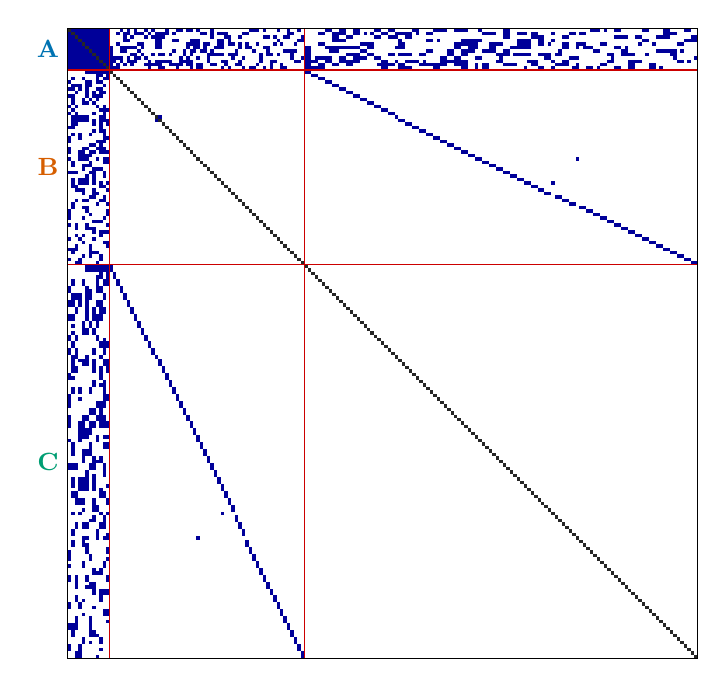
\begin{tikzpicture}[scale=1.0]
  \fill[black!85] (0.000,0.000) rectangle (0.044,-0.044);
  \fill[blue!60!black] (0.044,0.000) rectangle (0.088,-0.044);
  \fill[blue!60!black] (0.088,0.000) rectangle (0.133,-0.044);
  \fill[blue!60!black] (0.133,0.000) rectangle (0.177,-0.044);
  \fill[blue!60!black] (0.177,0.000) rectangle (0.221,-0.044);
  \fill[blue!60!black] (0.221,0.000) rectangle (0.265,-0.044);
  \fill[blue!60!black] (0.265,0.000) rectangle (0.309,-0.044);
  \fill[blue!60!black] (0.309,0.000) rectangle (0.354,-0.044);
  \fill[blue!60!black] (0.354,0.000) rectangle (0.398,-0.044);
  \fill[blue!60!black] (0.398,0.000) rectangle (0.442,-0.044);
  \fill[blue!60!black] (0.442,0.000) rectangle (0.486,-0.044);
  \fill[blue!60!black] (0.486,0.000) rectangle (0.530,-0.044);
  \fill[blue!60!black] (0.663,0.000) rectangle (0.707,-0.044);
  \fill[blue!60!black] (0.751,0.000) rectangle (0.796,-0.044);
  \fill[blue!60!black] (0.840,0.000) rectangle (0.884,-0.044);
  \fill[blue!60!black] (0.972,0.000) rectangle (1.017,-0.044);
  \fill[blue!60!black] (1.061,0.000) rectangle (1.105,-0.044);
  \fill[blue!60!black] (1.238,0.000) rectangle (1.282,-0.044);
  \fill[blue!60!black] (1.370,0.000) rectangle (1.414,-0.044);
  \fill[blue!60!black] (1.414,0.000) rectangle (1.459,-0.044);
  \fill[blue!60!black] (1.503,0.000) rectangle (1.547,-0.044);
  \fill[blue!60!black] (1.547,0.000) rectangle (1.591,-0.044);
  \fill[blue!60!black] (1.635,0.000) rectangle (1.680,-0.044);
  \fill[blue!60!black] (1.812,0.000) rectangle (1.856,-0.044);
  \fill[blue!60!black] (2.298,0.000) rectangle (2.343,-0.044);
  \fill[blue!60!black] (2.343,0.000) rectangle (2.387,-0.044);
  \fill[blue!60!black] (2.387,0.000) rectangle (2.431,-0.044);
  \fill[blue!60!black] (2.475,0.000) rectangle (2.519,-0.044);
  \fill[blue!60!black] (2.652,0.000) rectangle (2.696,-0.044);
  \fill[blue!60!black] (2.785,0.000) rectangle (2.829,-0.044);
  \fill[blue!60!black] (2.917,0.000) rectangle (2.961,-0.044);
  \fill[blue!60!black] (3.271,0.000) rectangle (3.315,-0.044);
  \fill[blue!60!black] (3.315,0.000) rectangle (3.359,-0.044);
  \fill[blue!60!black] (3.448,0.000) rectangle (3.492,-0.044);
  \fill[blue!60!black] (3.492,0.000) rectangle (3.536,-0.044);
  \fill[blue!60!black] (3.624,0.000) rectangle (3.669,-0.044);
  \fill[blue!60!black] (3.669,0.000) rectangle (3.713,-0.044);
  \fill[blue!60!black] (3.890,0.000) rectangle (3.934,-0.044);
  \fill[blue!60!black] (3.934,0.000) rectangle (3.978,-0.044);
  \fill[blue!60!black] (4.066,0.000) rectangle (4.110,-0.044);
  \fill[blue!60!black] (4.110,0.000) rectangle (4.155,-0.044);
  \fill[blue!60!black] (4.376,0.000) rectangle (4.420,-0.044);
  \fill[blue!60!black] (4.420,0.000) rectangle (4.464,-0.044);
  \fill[blue!60!black] (4.641,0.000) rectangle (4.685,-0.044);
  \fill[blue!60!black] (4.685,0.000) rectangle (4.729,-0.044);
  \fill[blue!60!black] (4.729,0.000) rectangle (4.773,-0.044);
  \fill[blue!60!black] (4.773,0.000) rectangle (4.818,-0.044);
  \fill[blue!60!black] (4.906,0.000) rectangle (4.950,-0.044);
  \fill[blue!60!black] (4.950,0.000) rectangle (4.994,-0.044);
  \fill[blue!60!black] (4.994,0.000) rectangle (5.039,-0.044);
  \fill[blue!60!black] (5.039,0.000) rectangle (5.083,-0.044);
  \fill[blue!60!black] (5.215,0.000) rectangle (5.260,-0.044);
  \fill[blue!60!black] (5.525,0.000) rectangle (5.569,-0.044);
  \fill[blue!60!black] (5.569,0.000) rectangle (5.613,-0.044);
  \fill[blue!60!black] (6.630,0.000) rectangle (6.674,-0.044);
  \fill[blue!60!black] (6.674,0.000) rectangle (6.718,-0.044);
  \fill[blue!60!black] (6.718,0.000) rectangle (6.762,-0.044);
  \fill[blue!60!black] (6.807,0.000) rectangle (6.851,-0.044);
  \fill[blue!60!black] (6.939,0.000) rectangle (6.983,-0.044);
  \fill[blue!60!black] (6.983,0.000) rectangle (7.028,-0.044);
  \fill[blue!60!black] (7.293,0.000) rectangle (7.337,-0.044);
  \fill[blue!60!black] (7.337,0.000) rectangle (7.381,-0.044);
  \fill[blue!60!black] (7.558,0.000) rectangle (7.602,-0.044);
  \fill[blue!60!black] (7.602,0.000) rectangle (7.646,-0.044);
  \fill[blue!60!black] (7.823,0.000) rectangle (7.867,-0.044);
  \fill[blue!60!black] (7.867,0.000) rectangle (7.912,-0.044);
  \fill[blue!60!black] (0.000,-0.044) rectangle (0.044,-0.088);
  \fill[black!85] (0.044,-0.044) rectangle (0.088,-0.088);
  \fill[blue!60!black] (0.088,-0.044) rectangle (0.133,-0.088);
  \fill[blue!60!black] (0.133,-0.044) rectangle (0.177,-0.088);
  \fill[blue!60!black] (0.177,-0.044) rectangle (0.221,-0.088);
  \fill[blue!60!black] (0.221,-0.044) rectangle (0.265,-0.088);
  \fill[blue!60!black] (0.265,-0.044) rectangle (0.309,-0.088);
  \fill[blue!60!black] (0.309,-0.044) rectangle (0.354,-0.088);
  \fill[blue!60!black] (0.354,-0.044) rectangle (0.398,-0.088);
  \fill[blue!60!black] (0.398,-0.044) rectangle (0.442,-0.088);
  \fill[blue!60!black] (0.442,-0.044) rectangle (0.486,-0.088);
  \fill[blue!60!black] (0.486,-0.044) rectangle (0.530,-0.088);
  \fill[blue!60!black] (0.619,-0.044) rectangle (0.663,-0.088);
  \fill[blue!60!black] (0.707,-0.044) rectangle (0.751,-0.088);
  \fill[blue!60!black] (0.751,-0.044) rectangle (0.796,-0.088);
  \fill[blue!60!black] (0.840,-0.044) rectangle (0.884,-0.088);
  \fill[blue!60!black] (0.884,-0.044) rectangle (0.928,-0.088);
  \fill[blue!60!black] (0.928,-0.044) rectangle (0.972,-0.088);
  \fill[blue!60!black] (1.017,-0.044) rectangle (1.061,-0.088);
  \fill[blue!60!black] (1.105,-0.044) rectangle (1.149,-0.088);
  \fill[blue!60!black] (1.149,-0.044) rectangle (1.193,-0.088);
  \fill[blue!60!black] (1.193,-0.044) rectangle (1.238,-0.088);
  \fill[blue!60!black] (1.238,-0.044) rectangle (1.282,-0.088);
  \fill[blue!60!black] (1.326,-0.044) rectangle (1.370,-0.088);
  \fill[blue!60!black] (1.680,-0.044) rectangle (1.724,-0.088);
  \fill[blue!60!black] (1.724,-0.044) rectangle (1.768,-0.088);
  \fill[blue!60!black] (1.812,-0.044) rectangle (1.856,-0.088);
  \fill[blue!60!black] (1.901,-0.044) rectangle (1.945,-0.088);
  \fill[blue!60!black] (1.945,-0.044) rectangle (1.989,-0.088);
  \fill[blue!60!black] (1.989,-0.044) rectangle (2.033,-0.088);
  \fill[blue!60!black] (2.210,-0.044) rectangle (2.254,-0.088);
  \fill[blue!60!black] (2.254,-0.044) rectangle (2.298,-0.088);
  \fill[blue!60!black] (2.785,-0.044) rectangle (2.829,-0.088);
  \fill[blue!60!black] (2.829,-0.044) rectangle (2.873,-0.088);
  \fill[blue!60!black] (3.182,-0.044) rectangle (3.227,-0.088);
  \fill[blue!60!black] (3.227,-0.044) rectangle (3.271,-0.088);
  \fill[blue!60!black] (3.359,-0.044) rectangle (3.403,-0.088);
  \fill[blue!60!black] (3.403,-0.044) rectangle (3.448,-0.088);
  \fill[blue!60!black] (3.448,-0.044) rectangle (3.492,-0.088);
  \fill[blue!60!black] (3.492,-0.044) rectangle (3.536,-0.088);
  \fill[blue!60!black] (3.624,-0.044) rectangle (3.669,-0.088);
  \fill[blue!60!black] (3.669,-0.044) rectangle (3.713,-0.088);
  \fill[blue!60!black] (3.757,-0.044) rectangle (3.801,-0.088);
  \fill[blue!60!black] (3.845,-0.044) rectangle (3.890,-0.088);
  \fill[blue!60!black] (3.978,-0.044) rectangle (4.022,-0.088);
  \fill[blue!60!black] (4.022,-0.044) rectangle (4.066,-0.088);
  \fill[blue!60!black] (4.155,-0.044) rectangle (4.199,-0.088);
  \fill[blue!60!black] (4.199,-0.044) rectangle (4.243,-0.088);
  \fill[blue!60!black] (4.243,-0.044) rectangle (4.287,-0.088);
  \fill[blue!60!black] (4.287,-0.044) rectangle (4.331,-0.088);
  \fill[blue!60!black] (4.331,-0.044) rectangle (4.376,-0.088);
  \fill[blue!60!black] (4.420,-0.044) rectangle (4.464,-0.088);
  \fill[blue!60!black] (4.552,-0.044) rectangle (4.597,-0.088);
  \fill[blue!60!black] (4.597,-0.044) rectangle (4.641,-0.088);
  \fill[blue!60!black] (5.260,-0.044) rectangle (5.304,-0.088);
  \fill[blue!60!black] (5.304,-0.044) rectangle (5.348,-0.088);
  \fill[blue!60!black] (5.348,-0.044) rectangle (5.392,-0.088);
  \fill[blue!60!black] (5.392,-0.044) rectangle (5.436,-0.088);
  \fill[blue!60!black] (5.525,-0.044) rectangle (5.569,-0.088);
  \fill[blue!60!black] (5.569,-0.044) rectangle (5.613,-0.088);
  \fill[blue!60!black] (5.702,-0.044) rectangle (5.746,-0.088);
  \fill[blue!60!black] (5.746,-0.044) rectangle (5.790,-0.088);
  \fill[blue!60!black] (5.790,-0.044) rectangle (5.834,-0.088);
  \fill[blue!60!black] (5.878,-0.044) rectangle (5.923,-0.088);
  \fill[blue!60!black] (5.923,-0.044) rectangle (5.967,-0.088);
  \fill[blue!60!black] (6.144,-0.044) rectangle (6.188,-0.088);
  \fill[blue!60!black] (6.365,-0.044) rectangle (6.409,-0.088);
  \fill[blue!60!black] (6.409,-0.044) rectangle (6.453,-0.088);
  \fill[blue!60!black] (6.497,-0.044) rectangle (6.541,-0.088);
  \fill[blue!60!black] (6.541,-0.044) rectangle (6.586,-0.088);
  \fill[blue!60!black] (7.558,-0.044) rectangle (7.602,-0.088);
  \fill[blue!60!black] (7.602,-0.044) rectangle (7.646,-0.088);
  \fill[blue!60!black] (7.646,-0.044) rectangle (7.691,-0.088);
  \fill[blue!60!black] (7.691,-0.044) rectangle (7.735,-0.088);
  \fill[blue!60!black] (0.000,-0.088) rectangle (0.044,-0.133);
  \fill[blue!60!black] (0.044,-0.088) rectangle (0.088,-0.133);
  \fill[black!85] (0.088,-0.088) rectangle (0.133,-0.133);
  \fill[blue!60!black] (0.133,-0.088) rectangle (0.177,-0.133);
  \fill[blue!60!black] (0.177,-0.088) rectangle (0.221,-0.133);
  \fill[blue!60!black] (0.221,-0.088) rectangle (0.265,-0.133);
  \fill[blue!60!black] (0.265,-0.088) rectangle (0.309,-0.133);
  \fill[blue!60!black] (0.309,-0.088) rectangle (0.354,-0.133);
  \fill[blue!60!black] (0.354,-0.088) rectangle (0.398,-0.133);
  \fill[blue!60!black] (0.398,-0.088) rectangle (0.442,-0.133);
  \fill[blue!60!black] (0.442,-0.088) rectangle (0.486,-0.133);
  \fill[blue!60!black] (0.486,-0.088) rectangle (0.530,-0.133);
  \fill[blue!60!black] (0.707,-0.088) rectangle (0.751,-0.133);
  \fill[blue!60!black] (0.796,-0.088) rectangle (0.840,-0.133);
  \fill[blue!60!black] (0.972,-0.088) rectangle (1.017,-0.133);
  \fill[blue!60!black] (1.061,-0.088) rectangle (1.105,-0.133);
  \fill[blue!60!black] (1.105,-0.088) rectangle (1.149,-0.133);
  \fill[blue!60!black] (1.149,-0.088) rectangle (1.193,-0.133);
  \fill[blue!60!black] (1.193,-0.088) rectangle (1.238,-0.133);
  \fill[blue!60!black] (1.812,-0.088) rectangle (1.856,-0.133);
  \fill[blue!60!black] (1.989,-0.088) rectangle (2.033,-0.133);
  \fill[blue!60!black] (2.033,-0.088) rectangle (2.077,-0.133);
  \fill[blue!60!black] (2.166,-0.088) rectangle (2.210,-0.133);
  \fill[blue!60!black] (2.475,-0.088) rectangle (2.519,-0.133);
  \fill[blue!60!black] (2.519,-0.088) rectangle (2.564,-0.133);
  \fill[blue!60!black] (2.608,-0.088) rectangle (2.652,-0.133);
  \fill[blue!60!black] (2.740,-0.088) rectangle (2.785,-0.133);
  \fill[blue!60!black] (2.785,-0.088) rectangle (2.829,-0.133);
  \fill[blue!60!black] (2.961,-0.088) rectangle (3.006,-0.133);
  \fill[blue!60!black] (3.359,-0.088) rectangle (3.403,-0.133);
  \fill[blue!60!black] (3.403,-0.088) rectangle (3.448,-0.133);
  \fill[blue!60!black] (3.536,-0.088) rectangle (3.580,-0.133);
  \fill[blue!60!black] (3.580,-0.088) rectangle (3.624,-0.133);
  \fill[blue!60!black] (3.890,-0.088) rectangle (3.934,-0.133);
  \fill[blue!60!black] (3.934,-0.088) rectangle (3.978,-0.133);
  \fill[blue!60!black] (4.066,-0.088) rectangle (4.110,-0.133);
  \fill[blue!60!black] (4.110,-0.088) rectangle (4.155,-0.133);
  \fill[blue!60!black] (4.155,-0.088) rectangle (4.199,-0.133);
  \fill[blue!60!black] (4.287,-0.088) rectangle (4.331,-0.133);
  \fill[blue!60!black] (4.331,-0.088) rectangle (4.376,-0.133);
  \fill[blue!60!black] (5.525,-0.088) rectangle (5.569,-0.133);
  \fill[blue!60!black] (5.569,-0.088) rectangle (5.613,-0.133);
  \fill[blue!60!black] (5.878,-0.088) rectangle (5.923,-0.133);
  \fill[blue!60!black] (5.923,-0.088) rectangle (5.967,-0.133);
  \fill[blue!60!black] (5.967,-0.088) rectangle (6.011,-0.133);
  \fill[blue!60!black] (6.011,-0.088) rectangle (6.055,-0.133);
  \fill[blue!60!black] (6.276,-0.088) rectangle (6.320,-0.133);
  \fill[blue!60!black] (6.320,-0.088) rectangle (6.365,-0.133);
  \fill[blue!60!black] (6.939,-0.088) rectangle (6.983,-0.133);
  \fill[blue!60!black] (6.983,-0.088) rectangle (7.028,-0.133);
  \fill[blue!60!black] (7.028,-0.088) rectangle (7.072,-0.133);
  \fill[blue!60!black] (7.072,-0.088) rectangle (7.116,-0.133);
  \fill[blue!60!black] (7.204,-0.088) rectangle (7.249,-0.133);
  \fill[blue!60!black] (7.249,-0.088) rectangle (7.293,-0.133);
  \fill[blue!60!black] (7.470,-0.088) rectangle (7.514,-0.133);
  \fill[blue!60!black] (7.514,-0.088) rectangle (7.558,-0.133);
  \fill[blue!60!black] (7.558,-0.088) rectangle (7.602,-0.133);
  \fill[blue!60!black] (7.602,-0.088) rectangle (7.646,-0.133);
  \fill[blue!60!black] (7.912,-0.088) rectangle (7.956,-0.133);
  \fill[blue!60!black] (7.956,-0.088) rectangle (8.000,-0.133);
  \fill[blue!60!black] (0.000,-0.133) rectangle (0.044,-0.177);
  \fill[blue!60!black] (0.044,-0.133) rectangle (0.088,-0.177);
  \fill[blue!60!black] (0.088,-0.133) rectangle (0.133,-0.177);
  \fill[black!85] (0.133,-0.133) rectangle (0.177,-0.177);
  \fill[blue!60!black] (0.177,-0.133) rectangle (0.221,-0.177);
  \fill[blue!60!black] (0.221,-0.133) rectangle (0.265,-0.177);
  \fill[blue!60!black] (0.265,-0.133) rectangle (0.309,-0.177);
  \fill[blue!60!black] (0.309,-0.133) rectangle (0.354,-0.177);
  \fill[blue!60!black] (0.354,-0.133) rectangle (0.398,-0.177);
  \fill[blue!60!black] (0.398,-0.133) rectangle (0.442,-0.177);
  \fill[blue!60!black] (0.442,-0.133) rectangle (0.486,-0.177);
  \fill[blue!60!black] (0.486,-0.133) rectangle (0.530,-0.177);
  \fill[blue!60!black] (0.707,-0.133) rectangle (0.751,-0.177);
  \fill[blue!60!black] (0.751,-0.133) rectangle (0.796,-0.177);
  \fill[blue!60!black] (1.105,-0.133) rectangle (1.149,-0.177);
  \fill[blue!60!black] (1.149,-0.133) rectangle (1.193,-0.177);
  \fill[blue!60!black] (1.326,-0.133) rectangle (1.370,-0.177);
  \fill[blue!60!black] (1.370,-0.133) rectangle (1.414,-0.177);
  \fill[blue!60!black] (1.547,-0.133) rectangle (1.591,-0.177);
  \fill[blue!60!black] (1.591,-0.133) rectangle (1.635,-0.177);
  \fill[blue!60!black] (1.635,-0.133) rectangle (1.680,-0.177);
  \fill[blue!60!black] (1.901,-0.133) rectangle (1.945,-0.177);
  \fill[blue!60!black] (1.945,-0.133) rectangle (1.989,-0.177);
  \fill[blue!60!black] (2.033,-0.133) rectangle (2.077,-0.177);
  \fill[blue!60!black] (2.652,-0.133) rectangle (2.696,-0.177);
  \fill[blue!60!black] (2.917,-0.133) rectangle (2.961,-0.177);
  \fill[blue!60!black] (2.961,-0.133) rectangle (3.006,-0.177);
  \fill[blue!60!black] (3.359,-0.133) rectangle (3.403,-0.177);
  \fill[blue!60!black] (3.403,-0.133) rectangle (3.448,-0.177);
  \fill[blue!60!black] (3.448,-0.133) rectangle (3.492,-0.177);
  \fill[blue!60!black] (3.492,-0.133) rectangle (3.536,-0.177);
  \fill[blue!60!black] (4.199,-0.133) rectangle (4.243,-0.177);
  \fill[blue!60!black] (4.552,-0.133) rectangle (4.597,-0.177);
  \fill[blue!60!black] (4.597,-0.133) rectangle (4.641,-0.177);
  \fill[blue!60!black] (4.685,-0.133) rectangle (4.729,-0.177);
  \fill[blue!60!black] (4.994,-0.133) rectangle (5.039,-0.177);
  \fill[blue!60!black] (5.039,-0.133) rectangle (5.083,-0.177);
  \fill[blue!60!black] (5.083,-0.133) rectangle (5.127,-0.177);
  \fill[blue!60!black] (5.127,-0.133) rectangle (5.171,-0.177);
  \fill[blue!60!black] (5.171,-0.133) rectangle (5.215,-0.177);
  \fill[blue!60!black] (5.215,-0.133) rectangle (5.260,-0.177);
  \fill[blue!60!black] (5.702,-0.133) rectangle (5.746,-0.177);
  \fill[blue!60!black] (5.746,-0.133) rectangle (5.790,-0.177);
  \fill[blue!60!black] (5.790,-0.133) rectangle (5.834,-0.177);
  \fill[blue!60!black] (5.834,-0.133) rectangle (5.878,-0.177);
  \fill[blue!60!black] (5.967,-0.133) rectangle (6.011,-0.177);
  \fill[blue!60!black] (6.011,-0.133) rectangle (6.055,-0.177);
  \fill[blue!60!black] (6.144,-0.133) rectangle (6.188,-0.177);
  \fill[blue!60!black] (7.293,-0.133) rectangle (7.337,-0.177);
  \fill[blue!60!black] (7.337,-0.133) rectangle (7.381,-0.177);
  \fill[blue!60!black] (7.823,-0.133) rectangle (7.867,-0.177);
  \fill[blue!60!black] (7.867,-0.133) rectangle (7.912,-0.177);
  \fill[blue!60!black] (7.912,-0.133) rectangle (7.956,-0.177);
  \fill[blue!60!black] (7.956,-0.133) rectangle (8.000,-0.177);
  \fill[blue!60!black] (0.000,-0.177) rectangle (0.044,-0.221);
  \fill[blue!60!black] (0.044,-0.177) rectangle (0.088,-0.221);
  \fill[blue!60!black] (0.088,-0.177) rectangle (0.133,-0.221);
  \fill[blue!60!black] (0.133,-0.177) rectangle (0.177,-0.221);
  \fill[black!85] (0.177,-0.177) rectangle (0.221,-0.221);
  \fill[blue!60!black] (0.221,-0.177) rectangle (0.265,-0.221);
  \fill[blue!60!black] (0.265,-0.177) rectangle (0.309,-0.221);
  \fill[blue!60!black] (0.309,-0.177) rectangle (0.354,-0.221);
  \fill[blue!60!black] (0.354,-0.177) rectangle (0.398,-0.221);
  \fill[blue!60!black] (0.398,-0.177) rectangle (0.442,-0.221);
  \fill[blue!60!black] (0.442,-0.177) rectangle (0.486,-0.221);
  \fill[blue!60!black] (0.486,-0.177) rectangle (0.530,-0.221);
  \fill[blue!60!black] (0.619,-0.177) rectangle (0.663,-0.221);
  \fill[blue!60!black] (0.884,-0.177) rectangle (0.928,-0.221);
  \fill[blue!60!black] (0.928,-0.177) rectangle (0.972,-0.221);
  \fill[blue!60!black] (1.105,-0.177) rectangle (1.149,-0.221);
  \fill[blue!60!black] (1.149,-0.177) rectangle (1.193,-0.221);
  \fill[blue!60!black] (1.503,-0.177) rectangle (1.547,-0.221);
  \fill[blue!60!black] (1.547,-0.177) rectangle (1.591,-0.221);
  \fill[blue!60!black] (1.591,-0.177) rectangle (1.635,-0.221);
  \fill[blue!60!black] (1.635,-0.177) rectangle (1.680,-0.221);
  \fill[blue!60!black] (1.724,-0.177) rectangle (1.768,-0.221);
  \fill[blue!60!black] (1.768,-0.177) rectangle (1.812,-0.221);
  \fill[blue!60!black] (1.901,-0.177) rectangle (1.945,-0.221);
  \fill[blue!60!black] (1.945,-0.177) rectangle (1.989,-0.221);
  \fill[blue!60!black] (2.033,-0.177) rectangle (2.077,-0.221);
  \fill[blue!60!black] (2.077,-0.177) rectangle (2.122,-0.221);
  \fill[blue!60!black] (2.166,-0.177) rectangle (2.210,-0.221);
  \fill[blue!60!black] (2.254,-0.177) rectangle (2.298,-0.221);
  \fill[blue!60!black] (2.387,-0.177) rectangle (2.431,-0.221);
  \fill[blue!60!black] (2.608,-0.177) rectangle (2.652,-0.221);
  \fill[blue!60!black] (2.696,-0.177) rectangle (2.740,-0.221);
  \fill[blue!60!black] (2.873,-0.177) rectangle (2.917,-0.221);
  \fill[blue!60!black] (3.182,-0.177) rectangle (3.227,-0.221);
  \fill[blue!60!black] (3.227,-0.177) rectangle (3.271,-0.221);
  \fill[blue!60!black] (3.713,-0.177) rectangle (3.757,-0.221);
  \fill[blue!60!black] (3.757,-0.177) rectangle (3.801,-0.221);
  \fill[blue!60!black] (3.801,-0.177) rectangle (3.845,-0.221);
  \fill[blue!60!black] (3.845,-0.177) rectangle (3.890,-0.221);
  \fill[blue!60!black] (4.199,-0.177) rectangle (4.243,-0.221);
  \fill[blue!60!black] (4.243,-0.177) rectangle (4.287,-0.221);
  \fill[blue!60!black] (4.906,-0.177) rectangle (4.950,-0.221);
  \fill[blue!60!black] (4.950,-0.177) rectangle (4.994,-0.221);
  \fill[blue!60!black] (4.994,-0.177) rectangle (5.039,-0.221);
  \fill[blue!60!black] (5.039,-0.177) rectangle (5.083,-0.221);
  \fill[blue!60!black] (5.083,-0.177) rectangle (5.127,-0.221);
  \fill[blue!60!black] (5.127,-0.177) rectangle (5.171,-0.221);
  \fill[blue!60!black] (5.171,-0.177) rectangle (5.215,-0.221);
  \fill[blue!60!black] (5.348,-0.177) rectangle (5.392,-0.221);
  \fill[blue!60!black] (5.392,-0.177) rectangle (5.436,-0.221);
  \fill[blue!60!black] (5.436,-0.177) rectangle (5.481,-0.221);
  \fill[blue!60!black] (5.481,-0.177) rectangle (5.525,-0.221);
  \fill[blue!60!black] (5.702,-0.177) rectangle (5.746,-0.221);
  \fill[blue!60!black] (5.746,-0.177) rectangle (5.790,-0.221);
  \fill[blue!60!black] (5.790,-0.177) rectangle (5.834,-0.221);
  \fill[blue!60!black] (5.834,-0.177) rectangle (5.878,-0.221);
  \fill[blue!60!black] (5.967,-0.177) rectangle (6.011,-0.221);
  \fill[blue!60!black] (6.011,-0.177) rectangle (6.055,-0.221);
  \fill[blue!60!black] (6.099,-0.177) rectangle (6.144,-0.221);
  \fill[blue!60!black] (6.276,-0.177) rectangle (6.320,-0.221);
  \fill[blue!60!black] (6.320,-0.177) rectangle (6.365,-0.221);
  \fill[blue!60!black] (6.453,-0.177) rectangle (6.497,-0.221);
  \fill[blue!60!black] (6.497,-0.177) rectangle (6.541,-0.221);
  \fill[blue!60!black] (6.541,-0.177) rectangle (6.586,-0.221);
  \fill[blue!60!black] (6.762,-0.177) rectangle (6.807,-0.221);
  \fill[blue!60!black] (6.807,-0.177) rectangle (6.851,-0.221);
  \fill[blue!60!black] (7.249,-0.177) rectangle (7.293,-0.221);
  \fill[blue!60!black] (7.425,-0.177) rectangle (7.470,-0.221);
  \fill[blue!60!black] (7.735,-0.177) rectangle (7.779,-0.221);
  \fill[blue!60!black] (7.779,-0.177) rectangle (7.823,-0.221);
  \fill[blue!60!black] (0.000,-0.221) rectangle (0.044,-0.265);
  \fill[blue!60!black] (0.044,-0.221) rectangle (0.088,-0.265);
  \fill[blue!60!black] (0.088,-0.221) rectangle (0.133,-0.265);
  \fill[blue!60!black] (0.133,-0.221) rectangle (0.177,-0.265);
  \fill[blue!60!black] (0.177,-0.221) rectangle (0.221,-0.265);
  \fill[black!85] (0.221,-0.221) rectangle (0.265,-0.265);
  \fill[blue!60!black] (0.265,-0.221) rectangle (0.309,-0.265);
  \fill[blue!60!black] (0.309,-0.221) rectangle (0.354,-0.265);
  \fill[blue!60!black] (0.354,-0.221) rectangle (0.398,-0.265);
  \fill[blue!60!black] (0.398,-0.221) rectangle (0.442,-0.265);
  \fill[blue!60!black] (0.442,-0.221) rectangle (0.486,-0.265);
  \fill[blue!60!black] (0.486,-0.221) rectangle (0.530,-0.265);
  \fill[blue!60!black] (0.530,-0.221) rectangle (0.575,-0.265);
  \fill[blue!60!black] (0.663,-0.221) rectangle (0.707,-0.265);
  \fill[blue!60!black] (0.707,-0.221) rectangle (0.751,-0.265);
  \fill[blue!60!black] (0.751,-0.221) rectangle (0.796,-0.265);
  \fill[blue!60!black] (0.796,-0.221) rectangle (0.840,-0.265);
  \fill[blue!60!black] (0.840,-0.221) rectangle (0.884,-0.265);
  \fill[blue!60!black] (0.928,-0.221) rectangle (0.972,-0.265);
  \fill[blue!60!black] (1.105,-0.221) rectangle (1.149,-0.265);
  \fill[blue!60!black] (1.149,-0.221) rectangle (1.193,-0.265);
  \fill[blue!60!black] (1.503,-0.221) rectangle (1.547,-0.265);
  \fill[blue!60!black] (1.591,-0.221) rectangle (1.635,-0.265);
  \fill[blue!60!black] (1.635,-0.221) rectangle (1.680,-0.265);
  \fill[blue!60!black] (1.724,-0.221) rectangle (1.768,-0.265);
  \fill[blue!60!black] (1.856,-0.221) rectangle (1.901,-0.265);
  \fill[blue!60!black] (1.901,-0.221) rectangle (1.945,-0.265);
  \fill[blue!60!black] (1.945,-0.221) rectangle (1.989,-0.265);
  \fill[blue!60!black] (2.166,-0.221) rectangle (2.210,-0.265);
  \fill[blue!60!black] (2.254,-0.221) rectangle (2.298,-0.265);
  \fill[blue!60!black] (2.298,-0.221) rectangle (2.343,-0.265);
  \fill[blue!60!black] (2.475,-0.221) rectangle (2.519,-0.265);
  \fill[blue!60!black] (2.519,-0.221) rectangle (2.564,-0.265);
  \fill[blue!60!black] (3.006,-0.221) rectangle (3.050,-0.265);
  \fill[blue!60!black] (3.050,-0.221) rectangle (3.094,-0.265);
  \fill[blue!60!black] (3.271,-0.221) rectangle (3.315,-0.265);
  \fill[blue!60!black] (3.315,-0.221) rectangle (3.359,-0.265);
  \fill[blue!60!black] (3.359,-0.221) rectangle (3.403,-0.265);
  \fill[blue!60!black] (3.403,-0.221) rectangle (3.448,-0.265);
  \fill[blue!60!black] (3.448,-0.221) rectangle (3.492,-0.265);
  \fill[blue!60!black] (3.492,-0.221) rectangle (3.536,-0.265);
  \fill[blue!60!black] (3.536,-0.221) rectangle (3.580,-0.265);
  \fill[blue!60!black] (3.580,-0.221) rectangle (3.624,-0.265);
  \fill[blue!60!black] (3.624,-0.221) rectangle (3.669,-0.265);
  \fill[blue!60!black] (3.669,-0.221) rectangle (3.713,-0.265);
  \fill[blue!60!black] (3.801,-0.221) rectangle (3.845,-0.265);
  \fill[blue!60!black] (3.845,-0.221) rectangle (3.890,-0.265);
  \fill[blue!60!black] (4.155,-0.221) rectangle (4.199,-0.265);
  \fill[blue!60!black] (4.199,-0.221) rectangle (4.243,-0.265);
  \fill[blue!60!black] (4.243,-0.221) rectangle (4.287,-0.265);
  \fill[blue!60!black] (4.906,-0.221) rectangle (4.950,-0.265);
  \fill[blue!60!black] (4.950,-0.221) rectangle (4.994,-0.265);
  \fill[blue!60!black] (5.083,-0.221) rectangle (5.127,-0.265);
  \fill[blue!60!black] (5.127,-0.221) rectangle (5.171,-0.265);
  \fill[blue!60!black] (5.171,-0.221) rectangle (5.215,-0.265);
  \fill[blue!60!black] (5.348,-0.221) rectangle (5.392,-0.265);
  \fill[blue!60!black] (5.392,-0.221) rectangle (5.436,-0.265);
  \fill[blue!60!black] (5.613,-0.221) rectangle (5.657,-0.265);
  \fill[blue!60!black] (5.657,-0.221) rectangle (5.702,-0.265);
  \fill[blue!60!black] (5.702,-0.221) rectangle (5.746,-0.265);
  \fill[blue!60!black] (5.746,-0.221) rectangle (5.790,-0.265);
  \fill[blue!60!black] (5.790,-0.221) rectangle (5.834,-0.265);
  \fill[blue!60!black] (5.834,-0.221) rectangle (5.878,-0.265);
  \fill[blue!60!black] (6.276,-0.221) rectangle (6.320,-0.265);
  \fill[blue!60!black] (6.320,-0.221) rectangle (6.365,-0.265);
  \fill[blue!60!black] (6.453,-0.221) rectangle (6.497,-0.265);
  \fill[blue!60!black] (6.541,-0.221) rectangle (6.586,-0.265);
  \fill[blue!60!black] (6.586,-0.221) rectangle (6.630,-0.265);
  \fill[blue!60!black] (6.630,-0.221) rectangle (6.674,-0.265);
  \fill[blue!60!black] (6.939,-0.221) rectangle (6.983,-0.265);
  \fill[blue!60!black] (6.983,-0.221) rectangle (7.028,-0.265);
  \fill[blue!60!black] (7.072,-0.221) rectangle (7.116,-0.265);
  \fill[blue!60!black] (0.000,-0.265) rectangle (0.044,-0.309);
  \fill[blue!60!black] (0.044,-0.265) rectangle (0.088,-0.309);
  \fill[blue!60!black] (0.088,-0.265) rectangle (0.133,-0.309);
  \fill[blue!60!black] (0.133,-0.265) rectangle (0.177,-0.309);
  \fill[blue!60!black] (0.177,-0.265) rectangle (0.221,-0.309);
  \fill[blue!60!black] (0.221,-0.265) rectangle (0.265,-0.309);
  \fill[black!85] (0.265,-0.265) rectangle (0.309,-0.309);
  \fill[blue!60!black] (0.309,-0.265) rectangle (0.354,-0.309);
  \fill[blue!60!black] (0.354,-0.265) rectangle (0.398,-0.309);
  \fill[blue!60!black] (0.398,-0.265) rectangle (0.442,-0.309);
  \fill[blue!60!black] (0.442,-0.265) rectangle (0.486,-0.309);
  \fill[blue!60!black] (0.486,-0.265) rectangle (0.530,-0.309);
  \fill[blue!60!black] (0.530,-0.265) rectangle (0.575,-0.309);
  \fill[blue!60!black] (0.663,-0.265) rectangle (0.707,-0.309);
  \fill[blue!60!black] (0.707,-0.265) rectangle (0.751,-0.309);
  \fill[blue!60!black] (0.884,-0.265) rectangle (0.928,-0.309);
  \fill[blue!60!black] (1.326,-0.265) rectangle (1.370,-0.309);
  \fill[blue!60!black] (1.459,-0.265) rectangle (1.503,-0.309);
  \fill[blue!60!black] (1.547,-0.265) rectangle (1.591,-0.309);
  \fill[blue!60!black] (1.591,-0.265) rectangle (1.635,-0.309);
  \fill[blue!60!black] (1.680,-0.265) rectangle (1.724,-0.309);
  \fill[blue!60!black] (1.724,-0.265) rectangle (1.768,-0.309);
  \fill[blue!60!black] (1.812,-0.265) rectangle (1.856,-0.309);
  \fill[blue!60!black] (2.122,-0.265) rectangle (2.166,-0.309);
  \fill[blue!60!black] (2.343,-0.265) rectangle (2.387,-0.309);
  \fill[blue!60!black] (2.519,-0.265) rectangle (2.564,-0.309);
  \fill[blue!60!black] (2.740,-0.265) rectangle (2.785,-0.309);
  \fill[blue!60!black] (2.785,-0.265) rectangle (2.829,-0.309);
  \fill[blue!60!black] (2.829,-0.265) rectangle (2.873,-0.309);
  \fill[blue!60!black] (2.873,-0.265) rectangle (2.917,-0.309);
  \fill[blue!60!black] (3.006,-0.265) rectangle (3.050,-0.309);
  \fill[blue!60!black] (3.050,-0.265) rectangle (3.094,-0.309);
  \fill[blue!60!black] (3.315,-0.265) rectangle (3.359,-0.309);
  \fill[blue!60!black] (3.359,-0.265) rectangle (3.403,-0.309);
  \fill[blue!60!black] (3.403,-0.265) rectangle (3.448,-0.309);
  \fill[blue!60!black] (3.713,-0.265) rectangle (3.757,-0.309);
  \fill[blue!60!black] (3.757,-0.265) rectangle (3.801,-0.309);
  \fill[blue!60!black] (4.552,-0.265) rectangle (4.597,-0.309);
  \fill[blue!60!black] (4.597,-0.265) rectangle (4.641,-0.309);
  \fill[blue!60!black] (4.818,-0.265) rectangle (4.862,-0.309);
  \fill[blue!60!black] (4.862,-0.265) rectangle (4.906,-0.309);
  \fill[blue!60!black] (4.994,-0.265) rectangle (5.039,-0.309);
  \fill[blue!60!black] (5.039,-0.265) rectangle (5.083,-0.309);
  \fill[blue!60!black] (5.083,-0.265) rectangle (5.127,-0.309);
  \fill[blue!60!black] (5.127,-0.265) rectangle (5.171,-0.309);
  \fill[blue!60!black] (5.260,-0.265) rectangle (5.304,-0.309);
  \fill[blue!60!black] (5.304,-0.265) rectangle (5.348,-0.309);
  \fill[blue!60!black] (5.348,-0.265) rectangle (5.392,-0.309);
  \fill[blue!60!black] (5.392,-0.265) rectangle (5.436,-0.309);
  \fill[blue!60!black] (5.525,-0.265) rectangle (5.569,-0.309);
  \fill[blue!60!black] (5.569,-0.265) rectangle (5.613,-0.309);
  \fill[blue!60!black] (6.232,-0.265) rectangle (6.276,-0.309);
  \fill[blue!60!black] (6.674,-0.265) rectangle (6.718,-0.309);
  \fill[blue!60!black] (6.718,-0.265) rectangle (6.762,-0.309);
  \fill[blue!60!black] (7.028,-0.265) rectangle (7.072,-0.309);
  \fill[blue!60!black] (7.072,-0.265) rectangle (7.116,-0.309);
  \fill[blue!60!black] (7.470,-0.265) rectangle (7.514,-0.309);
  \fill[blue!60!black] (7.514,-0.265) rectangle (7.558,-0.309);
  \fill[blue!60!black] (7.558,-0.265) rectangle (7.602,-0.309);
  \fill[blue!60!black] (7.602,-0.265) rectangle (7.646,-0.309);
  \fill[blue!60!black] (7.646,-0.265) rectangle (7.691,-0.309);
  \fill[blue!60!black] (7.691,-0.265) rectangle (7.735,-0.309);
  \fill[blue!60!black] (7.779,-0.265) rectangle (7.823,-0.309);
  \fill[blue!60!black] (0.000,-0.309) rectangle (0.044,-0.354);
  \fill[blue!60!black] (0.044,-0.309) rectangle (0.088,-0.354);
  \fill[blue!60!black] (0.088,-0.309) rectangle (0.133,-0.354);
  \fill[blue!60!black] (0.133,-0.309) rectangle (0.177,-0.354);
  \fill[blue!60!black] (0.177,-0.309) rectangle (0.221,-0.354);
  \fill[blue!60!black] (0.221,-0.309) rectangle (0.265,-0.354);
  \fill[blue!60!black] (0.265,-0.309) rectangle (0.309,-0.354);
  \fill[black!85] (0.309,-0.309) rectangle (0.354,-0.354);
  \fill[blue!60!black] (0.354,-0.309) rectangle (0.398,-0.354);
  \fill[blue!60!black] (0.398,-0.309) rectangle (0.442,-0.354);
  \fill[blue!60!black] (0.442,-0.309) rectangle (0.486,-0.354);
  \fill[blue!60!black] (0.486,-0.309) rectangle (0.530,-0.354);
  \fill[blue!60!black] (0.530,-0.309) rectangle (0.575,-0.354);
  \fill[blue!60!black] (0.796,-0.309) rectangle (0.840,-0.354);
  \fill[blue!60!black] (0.840,-0.309) rectangle (0.884,-0.354);
  \fill[blue!60!black] (0.928,-0.309) rectangle (0.972,-0.354);
  \fill[blue!60!black] (1.061,-0.309) rectangle (1.105,-0.354);
  \fill[blue!60!black] (1.149,-0.309) rectangle (1.193,-0.354);
  \fill[blue!60!black] (1.193,-0.309) rectangle (1.238,-0.354);
  \fill[blue!60!black] (1.282,-0.309) rectangle (1.326,-0.354);
  \fill[blue!60!black] (1.459,-0.309) rectangle (1.503,-0.354);
  \fill[blue!60!black] (1.547,-0.309) rectangle (1.591,-0.354);
  \fill[blue!60!black] (1.768,-0.309) rectangle (1.812,-0.354);
  \fill[blue!60!black] (1.812,-0.309) rectangle (1.856,-0.354);
  \fill[blue!60!black] (1.856,-0.309) rectangle (1.901,-0.354);
  \fill[blue!60!black] (1.901,-0.309) rectangle (1.945,-0.354);
  \fill[blue!60!black] (1.945,-0.309) rectangle (1.989,-0.354);
  \fill[blue!60!black] (2.033,-0.309) rectangle (2.077,-0.354);
  \fill[blue!60!black] (2.077,-0.309) rectangle (2.122,-0.354);
  \fill[blue!60!black] (2.122,-0.309) rectangle (2.166,-0.354);
  \fill[blue!60!black] (2.431,-0.309) rectangle (2.475,-0.354);
  \fill[blue!60!black] (2.519,-0.309) rectangle (2.564,-0.354);
  \fill[blue!60!black] (2.564,-0.309) rectangle (2.608,-0.354);
  \fill[blue!60!black] (2.652,-0.309) rectangle (2.696,-0.354);
  \fill[blue!60!black] (2.829,-0.309) rectangle (2.873,-0.354);
  \fill[blue!60!black] (3.006,-0.309) rectangle (3.050,-0.354);
  \fill[blue!60!black] (3.050,-0.309) rectangle (3.094,-0.354);
  \fill[blue!60!black] (3.536,-0.309) rectangle (3.580,-0.354);
  \fill[blue!60!black] (3.580,-0.309) rectangle (3.624,-0.354);
  \fill[blue!60!black] (3.624,-0.309) rectangle (3.669,-0.354);
  \fill[blue!60!black] (3.669,-0.309) rectangle (3.713,-0.354);
  \fill[blue!60!black] (3.801,-0.309) rectangle (3.845,-0.354);
  \fill[blue!60!black] (3.845,-0.309) rectangle (3.890,-0.354);
  \fill[blue!60!black] (4.066,-0.309) rectangle (4.110,-0.354);
  \fill[blue!60!black] (4.110,-0.309) rectangle (4.155,-0.354);
  \fill[blue!60!black] (4.199,-0.309) rectangle (4.243,-0.354);
  \fill[blue!60!black] (4.243,-0.309) rectangle (4.287,-0.354);
  \fill[blue!60!black] (4.287,-0.309) rectangle (4.331,-0.354);
  \fill[blue!60!black] (4.331,-0.309) rectangle (4.376,-0.354);
  \fill[blue!60!black] (4.464,-0.309) rectangle (4.508,-0.354);
  \fill[blue!60!black] (4.508,-0.309) rectangle (4.552,-0.354);
  \fill[blue!60!black] (4.818,-0.309) rectangle (4.862,-0.354);
  \fill[blue!60!black] (4.862,-0.309) rectangle (4.906,-0.354);
  \fill[blue!60!black] (4.994,-0.309) rectangle (5.039,-0.354);
  \fill[blue!60!black] (5.039,-0.309) rectangle (5.083,-0.354);
  \fill[blue!60!black] (5.436,-0.309) rectangle (5.481,-0.354);
  \fill[blue!60!black] (5.481,-0.309) rectangle (5.525,-0.354);
  \fill[blue!60!black] (5.525,-0.309) rectangle (5.569,-0.354);
  \fill[blue!60!black] (5.569,-0.309) rectangle (5.613,-0.354);
  \fill[blue!60!black] (5.657,-0.309) rectangle (5.702,-0.354);
  \fill[blue!60!black] (5.702,-0.309) rectangle (5.746,-0.354);
  \fill[blue!60!black] (5.746,-0.309) rectangle (5.790,-0.354);
  \fill[blue!60!black] (5.790,-0.309) rectangle (5.834,-0.354);
  \fill[blue!60!black] (5.834,-0.309) rectangle (5.878,-0.354);
  \fill[blue!60!black] (5.967,-0.309) rectangle (6.011,-0.354);
  \fill[blue!60!black] (6.011,-0.309) rectangle (6.055,-0.354);
  \fill[blue!60!black] (6.055,-0.309) rectangle (6.099,-0.354);
  \fill[blue!60!black] (6.099,-0.309) rectangle (6.144,-0.354);
  \fill[blue!60!black] (6.188,-0.309) rectangle (6.232,-0.354);
  \fill[blue!60!black] (6.232,-0.309) rectangle (6.276,-0.354);
  \fill[blue!60!black] (6.851,-0.309) rectangle (6.895,-0.354);
  \fill[blue!60!black] (6.895,-0.309) rectangle (6.939,-0.354);
  \fill[blue!60!black] (7.028,-0.309) rectangle (7.072,-0.354);
  \fill[blue!60!black] (7.072,-0.309) rectangle (7.116,-0.354);
  \fill[blue!60!black] (7.116,-0.309) rectangle (7.160,-0.354);
  \fill[blue!60!black] (7.160,-0.309) rectangle (7.204,-0.354);
  \fill[blue!60!black] (7.337,-0.309) rectangle (7.381,-0.354);
  \fill[blue!60!black] (7.646,-0.309) rectangle (7.691,-0.354);
  \fill[blue!60!black] (7.691,-0.309) rectangle (7.735,-0.354);
  \fill[blue!60!black] (0.000,-0.354) rectangle (0.044,-0.398);
  \fill[blue!60!black] (0.044,-0.354) rectangle (0.088,-0.398);
  \fill[blue!60!black] (0.088,-0.354) rectangle (0.133,-0.398);
  \fill[blue!60!black] (0.133,-0.354) rectangle (0.177,-0.398);
  \fill[blue!60!black] (0.177,-0.354) rectangle (0.221,-0.398);
  \fill[blue!60!black] (0.221,-0.354) rectangle (0.265,-0.398);
  \fill[blue!60!black] (0.265,-0.354) rectangle (0.309,-0.398);
  \fill[blue!60!black] (0.309,-0.354) rectangle (0.354,-0.398);
  \fill[black!85] (0.354,-0.354) rectangle (0.398,-0.398);
  \fill[blue!60!black] (0.398,-0.354) rectangle (0.442,-0.398);
  \fill[blue!60!black] (0.442,-0.354) rectangle (0.486,-0.398);
  \fill[blue!60!black] (0.486,-0.354) rectangle (0.530,-0.398);
  \fill[blue!60!black] (0.530,-0.354) rectangle (0.575,-0.398);
  \fill[blue!60!black] (0.575,-0.354) rectangle (0.619,-0.398);
  \fill[blue!60!black] (0.619,-0.354) rectangle (0.663,-0.398);
  \fill[blue!60!black] (0.663,-0.354) rectangle (0.707,-0.398);
  \fill[blue!60!black] (0.751,-0.354) rectangle (0.796,-0.398);
  \fill[blue!60!black] (0.840,-0.354) rectangle (0.884,-0.398);
  \fill[blue!60!black] (0.884,-0.354) rectangle (0.928,-0.398);
  \fill[blue!60!black] (0.972,-0.354) rectangle (1.017,-0.398);
  \fill[blue!60!black] (1.414,-0.354) rectangle (1.459,-0.398);
  \fill[blue!60!black] (1.503,-0.354) rectangle (1.547,-0.398);
  \fill[blue!60!black] (1.635,-0.354) rectangle (1.680,-0.398);
  \fill[blue!60!black] (1.768,-0.354) rectangle (1.812,-0.398);
  \fill[blue!60!black] (2.077,-0.354) rectangle (2.122,-0.398);
  \fill[blue!60!black] (2.210,-0.354) rectangle (2.254,-0.398);
  \fill[blue!60!black] (2.431,-0.354) rectangle (2.475,-0.398);
  \fill[blue!60!black] (2.829,-0.354) rectangle (2.873,-0.398);
  \fill[blue!60!black] (2.961,-0.354) rectangle (3.006,-0.398);
  \fill[blue!60!black] (3.006,-0.354) rectangle (3.050,-0.398);
  \fill[blue!60!black] (3.050,-0.354) rectangle (3.094,-0.398);
  \fill[blue!60!black] (3.138,-0.354) rectangle (3.182,-0.398);
  \fill[blue!60!black] (3.182,-0.354) rectangle (3.227,-0.398);
  \fill[blue!60!black] (3.227,-0.354) rectangle (3.271,-0.398);
  \fill[blue!60!black] (3.271,-0.354) rectangle (3.315,-0.398);
  \fill[blue!60!black] (3.315,-0.354) rectangle (3.359,-0.398);
  \fill[blue!60!black] (3.448,-0.354) rectangle (3.492,-0.398);
  \fill[blue!60!black] (3.492,-0.354) rectangle (3.536,-0.398);
  \fill[blue!60!black] (3.624,-0.354) rectangle (3.669,-0.398);
  \fill[blue!60!black] (3.669,-0.354) rectangle (3.713,-0.398);
  \fill[blue!60!black] (3.713,-0.354) rectangle (3.757,-0.398);
  \fill[blue!60!black] (3.757,-0.354) rectangle (3.801,-0.398);
  \fill[blue!60!black] (3.890,-0.354) rectangle (3.934,-0.398);
  \fill[blue!60!black] (3.934,-0.354) rectangle (3.978,-0.398);
  \fill[blue!60!black] (4.729,-0.354) rectangle (4.773,-0.398);
  \fill[blue!60!black] (4.773,-0.354) rectangle (4.818,-0.398);
  \fill[blue!60!black] (4.906,-0.354) rectangle (4.950,-0.398);
  \fill[blue!60!black] (4.950,-0.354) rectangle (4.994,-0.398);
  \fill[blue!60!black] (5.171,-0.354) rectangle (5.215,-0.398);
  \fill[blue!60!black] (5.215,-0.354) rectangle (5.260,-0.398);
  \fill[blue!60!black] (5.481,-0.354) rectangle (5.525,-0.398);
  \fill[blue!60!black] (6.055,-0.354) rectangle (6.099,-0.398);
  \fill[blue!60!black] (6.099,-0.354) rectangle (6.144,-0.398);
  \fill[blue!60!black] (6.365,-0.354) rectangle (6.409,-0.398);
  \fill[blue!60!black] (6.409,-0.354) rectangle (6.453,-0.398);
  \fill[blue!60!black] (6.453,-0.354) rectangle (6.497,-0.398);
  \fill[blue!60!black] (6.895,-0.354) rectangle (6.939,-0.398);
  \fill[blue!60!black] (7.691,-0.354) rectangle (7.735,-0.398);
  \fill[blue!60!black] (7.956,-0.354) rectangle (8.000,-0.398);
  \fill[blue!60!black] (0.000,-0.398) rectangle (0.044,-0.442);
  \fill[blue!60!black] (0.044,-0.398) rectangle (0.088,-0.442);
  \fill[blue!60!black] (0.088,-0.398) rectangle (0.133,-0.442);
  \fill[blue!60!black] (0.133,-0.398) rectangle (0.177,-0.442);
  \fill[blue!60!black] (0.177,-0.398) rectangle (0.221,-0.442);
  \fill[blue!60!black] (0.221,-0.398) rectangle (0.265,-0.442);
  \fill[blue!60!black] (0.265,-0.398) rectangle (0.309,-0.442);
  \fill[blue!60!black] (0.309,-0.398) rectangle (0.354,-0.442);
  \fill[blue!60!black] (0.354,-0.398) rectangle (0.398,-0.442);
  \fill[black!85] (0.398,-0.398) rectangle (0.442,-0.442);
  \fill[blue!60!black] (0.442,-0.398) rectangle (0.486,-0.442);
  \fill[blue!60!black] (0.486,-0.398) rectangle (0.530,-0.442);
  \fill[blue!60!black] (0.530,-0.398) rectangle (0.575,-0.442);
  \fill[blue!60!black] (0.575,-0.398) rectangle (0.619,-0.442);
  \fill[blue!60!black] (0.663,-0.398) rectangle (0.707,-0.442);
  \fill[blue!60!black] (0.751,-0.398) rectangle (0.796,-0.442);
  \fill[blue!60!black] (0.796,-0.398) rectangle (0.840,-0.442);
  \fill[blue!60!black] (0.840,-0.398) rectangle (0.884,-0.442);
  \fill[blue!60!black] (1.017,-0.398) rectangle (1.061,-0.442);
  \fill[blue!60!black] (1.105,-0.398) rectangle (1.149,-0.442);
  \fill[blue!60!black] (1.149,-0.398) rectangle (1.193,-0.442);
  \fill[blue!60!black] (1.193,-0.398) rectangle (1.238,-0.442);
  \fill[blue!60!black] (1.238,-0.398) rectangle (1.282,-0.442);
  \fill[blue!60!black] (1.282,-0.398) rectangle (1.326,-0.442);
  \fill[blue!60!black] (1.414,-0.398) rectangle (1.459,-0.442);
  \fill[blue!60!black] (1.459,-0.398) rectangle (1.503,-0.442);
  \fill[blue!60!black] (1.503,-0.398) rectangle (1.547,-0.442);
  \fill[blue!60!black] (1.547,-0.398) rectangle (1.591,-0.442);
  \fill[blue!60!black] (1.768,-0.398) rectangle (1.812,-0.442);
  \fill[blue!60!black] (1.945,-0.398) rectangle (1.989,-0.442);
  \fill[blue!60!black] (1.989,-0.398) rectangle (2.033,-0.442);
  \fill[blue!60!black] (2.166,-0.398) rectangle (2.210,-0.442);
  \fill[blue!60!black] (2.431,-0.398) rectangle (2.475,-0.442);
  \fill[blue!60!black] (2.564,-0.398) rectangle (2.608,-0.442);
  \fill[blue!60!black] (2.608,-0.398) rectangle (2.652,-0.442);
  \fill[blue!60!black] (2.873,-0.398) rectangle (2.917,-0.442);
  \fill[blue!60!black] (2.917,-0.398) rectangle (2.961,-0.442);
  \fill[blue!60!black] (3.006,-0.398) rectangle (3.050,-0.442);
  \fill[blue!60!black] (3.050,-0.398) rectangle (3.094,-0.442);
  \fill[blue!60!black] (3.094,-0.398) rectangle (3.138,-0.442);
  \fill[blue!60!black] (3.138,-0.398) rectangle (3.182,-0.442);
  \fill[blue!60!black] (3.271,-0.398) rectangle (3.315,-0.442);
  \fill[blue!60!black] (3.315,-0.398) rectangle (3.359,-0.442);
  \fill[blue!60!black] (3.448,-0.398) rectangle (3.492,-0.442);
  \fill[blue!60!black] (3.492,-0.398) rectangle (3.536,-0.442);
  \fill[blue!60!black] (3.536,-0.398) rectangle (3.580,-0.442);
  \fill[blue!60!black] (3.580,-0.398) rectangle (3.624,-0.442);
  \fill[blue!60!black] (3.624,-0.398) rectangle (3.669,-0.442);
  \fill[blue!60!black] (3.669,-0.398) rectangle (3.713,-0.442);
  \fill[blue!60!black] (3.978,-0.398) rectangle (4.022,-0.442);
  \fill[blue!60!black] (4.022,-0.398) rectangle (4.066,-0.442);
  \fill[blue!60!black] (4.155,-0.398) rectangle (4.199,-0.442);
  \fill[blue!60!black] (4.287,-0.398) rectangle (4.331,-0.442);
  \fill[blue!60!black] (4.331,-0.398) rectangle (4.376,-0.442);
  \fill[blue!60!black] (4.376,-0.398) rectangle (4.420,-0.442);
  \fill[blue!60!black] (4.420,-0.398) rectangle (4.464,-0.442);
  \fill[blue!60!black] (4.508,-0.398) rectangle (4.552,-0.442);
  \fill[blue!60!black] (4.729,-0.398) rectangle (4.773,-0.442);
  \fill[blue!60!black] (4.773,-0.398) rectangle (4.818,-0.442);
  \fill[blue!60!black] (4.818,-0.398) rectangle (4.862,-0.442);
  \fill[blue!60!black] (4.862,-0.398) rectangle (4.906,-0.442);
  \fill[blue!60!black] (4.906,-0.398) rectangle (4.950,-0.442);
  \fill[blue!60!black] (4.950,-0.398) rectangle (4.994,-0.442);
  \fill[blue!60!black] (4.994,-0.398) rectangle (5.039,-0.442);
  \fill[blue!60!black] (5.039,-0.398) rectangle (5.083,-0.442);
  \fill[blue!60!black] (5.436,-0.398) rectangle (5.481,-0.442);
  \fill[blue!60!black] (5.481,-0.398) rectangle (5.525,-0.442);
  \fill[blue!60!black] (5.834,-0.398) rectangle (5.878,-0.442);
  \fill[blue!60!black] (5.878,-0.398) rectangle (5.923,-0.442);
  \fill[blue!60!black] (5.923,-0.398) rectangle (5.967,-0.442);
  \fill[blue!60!black] (6.144,-0.398) rectangle (6.188,-0.442);
  \fill[blue!60!black] (6.276,-0.398) rectangle (6.320,-0.442);
  \fill[blue!60!black] (6.320,-0.398) rectangle (6.365,-0.442);
  \fill[blue!60!black] (6.851,-0.398) rectangle (6.895,-0.442);
  \fill[blue!60!black] (6.895,-0.398) rectangle (6.939,-0.442);
  \fill[blue!60!black] (7.116,-0.398) rectangle (7.160,-0.442);
  \fill[blue!60!black] (7.160,-0.398) rectangle (7.204,-0.442);
  \fill[blue!60!black] (7.204,-0.398) rectangle (7.249,-0.442);
  \fill[blue!60!black] (7.249,-0.398) rectangle (7.293,-0.442);
  \fill[blue!60!black] (7.735,-0.398) rectangle (7.779,-0.442);
  \fill[blue!60!black] (7.779,-0.398) rectangle (7.823,-0.442);
  \fill[blue!60!black] (7.867,-0.398) rectangle (7.912,-0.442);
  \fill[blue!60!black] (0.000,-0.442) rectangle (0.044,-0.486);
  \fill[blue!60!black] (0.044,-0.442) rectangle (0.088,-0.486);
  \fill[blue!60!black] (0.088,-0.442) rectangle (0.133,-0.486);
  \fill[blue!60!black] (0.133,-0.442) rectangle (0.177,-0.486);
  \fill[blue!60!black] (0.177,-0.442) rectangle (0.221,-0.486);
  \fill[blue!60!black] (0.221,-0.442) rectangle (0.265,-0.486);
  \fill[blue!60!black] (0.265,-0.442) rectangle (0.309,-0.486);
  \fill[blue!60!black] (0.309,-0.442) rectangle (0.354,-0.486);
  \fill[blue!60!black] (0.354,-0.442) rectangle (0.398,-0.486);
  \fill[blue!60!black] (0.398,-0.442) rectangle (0.442,-0.486);
  \fill[black!85] (0.442,-0.442) rectangle (0.486,-0.486);
  \fill[blue!60!black] (0.486,-0.442) rectangle (0.530,-0.486);
  \fill[blue!60!black] (0.530,-0.442) rectangle (0.575,-0.486);
  \fill[blue!60!black] (0.619,-0.442) rectangle (0.663,-0.486);
  \fill[blue!60!black] (0.707,-0.442) rectangle (0.751,-0.486);
  \fill[blue!60!black] (0.796,-0.442) rectangle (0.840,-0.486);
  \fill[blue!60!black] (0.972,-0.442) rectangle (1.017,-0.486);
  \fill[blue!60!black] (1.017,-0.442) rectangle (1.061,-0.486);
  \fill[blue!60!black] (1.061,-0.442) rectangle (1.105,-0.486);
  \fill[blue!60!black] (1.105,-0.442) rectangle (1.149,-0.486);
  \fill[blue!60!black] (1.149,-0.442) rectangle (1.193,-0.486);
  \fill[blue!60!black] (1.282,-0.442) rectangle (1.326,-0.486);
  \fill[blue!60!black] (1.326,-0.442) rectangle (1.370,-0.486);
  \fill[blue!60!black] (1.370,-0.442) rectangle (1.414,-0.486);
  \fill[blue!60!black] (1.414,-0.442) rectangle (1.459,-0.486);
  \fill[blue!60!black] (1.503,-0.442) rectangle (1.547,-0.486);
  \fill[blue!60!black] (1.547,-0.442) rectangle (1.591,-0.486);
  \fill[blue!60!black] (1.635,-0.442) rectangle (1.680,-0.486);
  \fill[blue!60!black] (1.680,-0.442) rectangle (1.724,-0.486);
  \fill[blue!60!black] (1.812,-0.442) rectangle (1.856,-0.486);
  \fill[blue!60!black] (1.856,-0.442) rectangle (1.901,-0.486);
  \fill[blue!60!black] (1.989,-0.442) rectangle (2.033,-0.486);
  \fill[blue!60!black] (2.122,-0.442) rectangle (2.166,-0.486);
  \fill[blue!60!black] (2.166,-0.442) rectangle (2.210,-0.486);
  \fill[blue!60!black] (2.387,-0.442) rectangle (2.431,-0.486);
  \fill[blue!60!black] (2.564,-0.442) rectangle (2.608,-0.486);
  \fill[blue!60!black] (2.696,-0.442) rectangle (2.740,-0.486);
  \fill[blue!60!black] (3.006,-0.442) rectangle (3.050,-0.486);
  \fill[blue!60!black] (3.050,-0.442) rectangle (3.094,-0.486);
  \fill[blue!60!black] (3.182,-0.442) rectangle (3.227,-0.486);
  \fill[blue!60!black] (3.227,-0.442) rectangle (3.271,-0.486);
  \fill[blue!60!black] (3.359,-0.442) rectangle (3.403,-0.486);
  \fill[blue!60!black] (3.403,-0.442) rectangle (3.448,-0.486);
  \fill[blue!60!black] (3.536,-0.442) rectangle (3.580,-0.486);
  \fill[blue!60!black] (3.580,-0.442) rectangle (3.624,-0.486);
  \fill[blue!60!black] (3.934,-0.442) rectangle (3.978,-0.486);
  \fill[blue!60!black] (3.978,-0.442) rectangle (4.022,-0.486);
  \fill[blue!60!black] (4.022,-0.442) rectangle (4.066,-0.486);
  \fill[blue!60!black] (4.066,-0.442) rectangle (4.110,-0.486);
  \fill[blue!60!black] (4.110,-0.442) rectangle (4.155,-0.486);
  \fill[blue!60!black] (4.199,-0.442) rectangle (4.243,-0.486);
  \fill[blue!60!black] (4.243,-0.442) rectangle (4.287,-0.486);
  \fill[blue!60!black] (4.464,-0.442) rectangle (4.508,-0.486);
  \fill[blue!60!black] (4.508,-0.442) rectangle (4.552,-0.486);
  \fill[blue!60!black] (4.552,-0.442) rectangle (4.597,-0.486);
  \fill[blue!60!black] (4.597,-0.442) rectangle (4.641,-0.486);
  \fill[blue!60!black] (4.641,-0.442) rectangle (4.685,-0.486);
  \fill[blue!60!black] (4.685,-0.442) rectangle (4.729,-0.486);
  \fill[blue!60!black] (4.729,-0.442) rectangle (4.773,-0.486);
  \fill[blue!60!black] (4.773,-0.442) rectangle (4.818,-0.486);
  \fill[blue!60!black] (4.906,-0.442) rectangle (4.950,-0.486);
  \fill[blue!60!black] (4.950,-0.442) rectangle (4.994,-0.486);
  \fill[blue!60!black] (4.994,-0.442) rectangle (5.039,-0.486);
  \fill[blue!60!black] (5.039,-0.442) rectangle (5.083,-0.486);
  \fill[blue!60!black] (5.171,-0.442) rectangle (5.215,-0.486);
  \fill[blue!60!black] (5.260,-0.442) rectangle (5.304,-0.486);
  \fill[blue!60!black] (5.304,-0.442) rectangle (5.348,-0.486);
  \fill[blue!60!black] (5.525,-0.442) rectangle (5.569,-0.486);
  \fill[blue!60!black] (5.569,-0.442) rectangle (5.613,-0.486);
  \fill[blue!60!black] (5.613,-0.442) rectangle (5.657,-0.486);
  \fill[blue!60!black] (5.657,-0.442) rectangle (5.702,-0.486);
  \fill[blue!60!black] (5.878,-0.442) rectangle (5.923,-0.486);
  \fill[blue!60!black] (5.923,-0.442) rectangle (5.967,-0.486);
  \fill[blue!60!black] (6.188,-0.442) rectangle (6.232,-0.486);
  \fill[blue!60!black] (6.232,-0.442) rectangle (6.276,-0.486);
  \fill[blue!60!black] (6.276,-0.442) rectangle (6.320,-0.486);
  \fill[blue!60!black] (6.320,-0.442) rectangle (6.365,-0.486);
  \fill[blue!60!black] (6.453,-0.442) rectangle (6.497,-0.486);
  \fill[blue!60!black] (6.762,-0.442) rectangle (6.807,-0.486);
  \fill[blue!60!black] (6.807,-0.442) rectangle (6.851,-0.486);
  \fill[blue!60!black] (7.116,-0.442) rectangle (7.160,-0.486);
  \fill[blue!60!black] (7.160,-0.442) rectangle (7.204,-0.486);
  \fill[blue!60!black] (7.381,-0.442) rectangle (7.425,-0.486);
  \fill[blue!60!black] (7.425,-0.442) rectangle (7.470,-0.486);
  \fill[blue!60!black] (0.000,-0.486) rectangle (0.044,-0.530);
  \fill[blue!60!black] (0.044,-0.486) rectangle (0.088,-0.530);
  \fill[blue!60!black] (0.088,-0.486) rectangle (0.133,-0.530);
  \fill[blue!60!black] (0.133,-0.486) rectangle (0.177,-0.530);
  \fill[blue!60!black] (0.177,-0.486) rectangle (0.221,-0.530);
  \fill[blue!60!black] (0.221,-0.486) rectangle (0.265,-0.530);
  \fill[blue!60!black] (0.265,-0.486) rectangle (0.309,-0.530);
  \fill[blue!60!black] (0.309,-0.486) rectangle (0.354,-0.530);
  \fill[blue!60!black] (0.354,-0.486) rectangle (0.398,-0.530);
  \fill[blue!60!black] (0.398,-0.486) rectangle (0.442,-0.530);
  \fill[blue!60!black] (0.442,-0.486) rectangle (0.486,-0.530);
  \fill[black!85] (0.486,-0.486) rectangle (0.530,-0.530);
  \fill[blue!60!black] (0.530,-0.486) rectangle (0.575,-0.530);
  \fill[blue!60!black] (0.575,-0.486) rectangle (0.619,-0.530);
  \fill[blue!60!black] (0.619,-0.486) rectangle (0.663,-0.530);
  \fill[blue!60!black] (1.017,-0.486) rectangle (1.061,-0.530);
  \fill[blue!60!black] (1.149,-0.486) rectangle (1.193,-0.530);
  \fill[blue!60!black] (1.193,-0.486) rectangle (1.238,-0.530);
  \fill[blue!60!black] (1.370,-0.486) rectangle (1.414,-0.530);
  \fill[blue!60!black] (1.547,-0.486) rectangle (1.591,-0.530);
  \fill[blue!60!black] (1.635,-0.486) rectangle (1.680,-0.530);
  \fill[blue!60!black] (1.680,-0.486) rectangle (1.724,-0.530);
  \fill[blue!60!black] (1.945,-0.486) rectangle (1.989,-0.530);
  \fill[blue!60!black] (2.033,-0.486) rectangle (2.077,-0.530);
  \fill[blue!60!black] (2.210,-0.486) rectangle (2.254,-0.530);
  \fill[blue!60!black] (2.298,-0.486) rectangle (2.343,-0.530);
  \fill[blue!60!black] (2.343,-0.486) rectangle (2.387,-0.530);
  \fill[blue!60!black] (2.475,-0.486) rectangle (2.519,-0.530);
  \fill[blue!60!black] (2.564,-0.486) rectangle (2.608,-0.530);
  \fill[blue!60!black] (2.696,-0.486) rectangle (2.740,-0.530);
  \fill[blue!60!black] (2.740,-0.486) rectangle (2.785,-0.530);
  \fill[blue!60!black] (3.006,-0.486) rectangle (3.050,-0.530);
  \fill[blue!60!black] (3.050,-0.486) rectangle (3.094,-0.530);
  \fill[blue!60!black] (3.094,-0.486) rectangle (3.138,-0.530);
  \fill[blue!60!black] (3.138,-0.486) rectangle (3.182,-0.530);
  \fill[blue!60!black] (3.182,-0.486) rectangle (3.227,-0.530);
  \fill[blue!60!black] (3.227,-0.486) rectangle (3.271,-0.530);
  \fill[blue!60!black] (3.978,-0.486) rectangle (4.022,-0.530);
  \fill[blue!60!black] (4.022,-0.486) rectangle (4.066,-0.530);
  \fill[blue!60!black] (4.199,-0.486) rectangle (4.243,-0.530);
  \fill[blue!60!black] (4.243,-0.486) rectangle (4.287,-0.530);
  \fill[blue!60!black] (4.287,-0.486) rectangle (4.331,-0.530);
  \fill[blue!60!black] (4.331,-0.486) rectangle (4.376,-0.530);
  \fill[blue!60!black] (4.641,-0.486) rectangle (4.685,-0.530);
  \fill[blue!60!black] (4.685,-0.486) rectangle (4.729,-0.530);
  \fill[blue!60!black] (4.994,-0.486) rectangle (5.039,-0.530);
  \fill[blue!60!black] (5.039,-0.486) rectangle (5.083,-0.530);
  \fill[blue!60!black] (5.171,-0.486) rectangle (5.215,-0.530);
  \fill[blue!60!black] (5.260,-0.486) rectangle (5.304,-0.530);
  \fill[blue!60!black] (5.304,-0.486) rectangle (5.348,-0.530);
  \fill[blue!60!black] (5.790,-0.486) rectangle (5.834,-0.530);
  \fill[blue!60!black] (5.967,-0.486) rectangle (6.011,-0.530);
  \fill[blue!60!black] (6.011,-0.486) rectangle (6.055,-0.530);
  \fill[blue!60!black] (6.144,-0.486) rectangle (6.188,-0.530);
  \fill[blue!60!black] (6.409,-0.486) rectangle (6.453,-0.530);
  \fill[blue!60!black] (6.453,-0.486) rectangle (6.497,-0.530);
  \fill[blue!60!black] (6.586,-0.486) rectangle (6.630,-0.530);
  \fill[blue!60!black] (6.630,-0.486) rectangle (6.674,-0.530);
  \fill[blue!60!black] (6.718,-0.486) rectangle (6.762,-0.530);
  \fill[blue!60!black] (6.939,-0.486) rectangle (6.983,-0.530);
  \fill[blue!60!black] (6.983,-0.486) rectangle (7.028,-0.530);
  \fill[blue!60!black] (7.116,-0.486) rectangle (7.160,-0.530);
  \fill[blue!60!black] (7.160,-0.486) rectangle (7.204,-0.530);
  \fill[blue!60!black] (7.381,-0.486) rectangle (7.425,-0.530);
  \fill[blue!60!black] (7.425,-0.486) rectangle (7.470,-0.530);
  \fill[blue!60!black] (7.514,-0.486) rectangle (7.558,-0.530);
  \fill[blue!60!black] (0.221,-0.530) rectangle (0.265,-0.575);
  \fill[blue!60!black] (0.265,-0.530) rectangle (0.309,-0.575);
  \fill[blue!60!black] (0.309,-0.530) rectangle (0.354,-0.575);
  \fill[blue!60!black] (0.354,-0.530) rectangle (0.398,-0.575);
  \fill[blue!60!black] (0.398,-0.530) rectangle (0.442,-0.575);
  \fill[blue!60!black] (0.442,-0.530) rectangle (0.486,-0.575);
  \fill[blue!60!black] (0.486,-0.530) rectangle (0.530,-0.575);
  \fill[black!85] (0.530,-0.530) rectangle (0.575,-0.575);
  \fill[blue!60!black] (3.006,-0.530) rectangle (3.050,-0.575);
  \fill[blue!60!black] (3.050,-0.530) rectangle (3.094,-0.575);
  \fill[blue!60!black] (0.354,-0.575) rectangle (0.398,-0.619);
  \fill[blue!60!black] (0.398,-0.575) rectangle (0.442,-0.619);
  \fill[blue!60!black] (0.486,-0.575) rectangle (0.530,-0.619);
  \fill[black!85] (0.575,-0.575) rectangle (0.619,-0.619);
  \fill[blue!60!black] (3.094,-0.575) rectangle (3.138,-0.619);
  \fill[blue!60!black] (3.138,-0.575) rectangle (3.182,-0.619);
  \fill[blue!60!black] (0.044,-0.619) rectangle (0.088,-0.663);
  \fill[blue!60!black] (0.177,-0.619) rectangle (0.221,-0.663);
  \fill[blue!60!black] (0.354,-0.619) rectangle (0.398,-0.663);
  \fill[blue!60!black] (0.442,-0.619) rectangle (0.486,-0.663);
  \fill[blue!60!black] (0.486,-0.619) rectangle (0.530,-0.663);
  \fill[black!85] (0.619,-0.619) rectangle (0.663,-0.663);
  \fill[blue!60!black] (3.182,-0.619) rectangle (3.227,-0.663);
  \fill[blue!60!black] (3.227,-0.619) rectangle (3.271,-0.663);
  \fill[blue!60!black] (0.000,-0.663) rectangle (0.044,-0.707);
  \fill[blue!60!black] (0.221,-0.663) rectangle (0.265,-0.707);
  \fill[blue!60!black] (0.265,-0.663) rectangle (0.309,-0.707);
  \fill[blue!60!black] (0.354,-0.663) rectangle (0.398,-0.707);
  \fill[blue!60!black] (0.398,-0.663) rectangle (0.442,-0.707);
  \fill[black!85] (0.663,-0.663) rectangle (0.707,-0.707);
  \fill[blue!60!black] (3.271,-0.663) rectangle (3.315,-0.707);
  \fill[blue!60!black] (3.315,-0.663) rectangle (3.359,-0.707);
  \fill[blue!60!black] (0.044,-0.707) rectangle (0.088,-0.751);
  \fill[blue!60!black] (0.088,-0.707) rectangle (0.133,-0.751);
  \fill[blue!60!black] (0.133,-0.707) rectangle (0.177,-0.751);
  \fill[blue!60!black] (0.221,-0.707) rectangle (0.265,-0.751);
  \fill[blue!60!black] (0.265,-0.707) rectangle (0.309,-0.751);
  \fill[blue!60!black] (0.442,-0.707) rectangle (0.486,-0.751);
  \fill[black!85] (0.707,-0.707) rectangle (0.751,-0.751);
  \fill[blue!60!black] (3.359,-0.707) rectangle (3.403,-0.751);
  \fill[blue!60!black] (3.403,-0.707) rectangle (3.448,-0.751);
  \fill[blue!60!black] (0.000,-0.751) rectangle (0.044,-0.796);
  \fill[blue!60!black] (0.044,-0.751) rectangle (0.088,-0.796);
  \fill[blue!60!black] (0.133,-0.751) rectangle (0.177,-0.796);
  \fill[blue!60!black] (0.221,-0.751) rectangle (0.265,-0.796);
  \fill[blue!60!black] (0.354,-0.751) rectangle (0.398,-0.796);
  \fill[blue!60!black] (0.398,-0.751) rectangle (0.442,-0.796);
  \fill[black!85] (0.751,-0.751) rectangle (0.796,-0.796);
  \fill[blue!60!black] (3.448,-0.751) rectangle (3.492,-0.796);
  \fill[blue!60!black] (3.492,-0.751) rectangle (3.536,-0.796);
  \fill[blue!60!black] (0.088,-0.796) rectangle (0.133,-0.840);
  \fill[blue!60!black] (0.221,-0.796) rectangle (0.265,-0.840);
  \fill[blue!60!black] (0.309,-0.796) rectangle (0.354,-0.840);
  \fill[blue!60!black] (0.398,-0.796) rectangle (0.442,-0.840);
  \fill[blue!60!black] (0.442,-0.796) rectangle (0.486,-0.840);
  \fill[black!85] (0.796,-0.796) rectangle (0.840,-0.840);
  \fill[blue!60!black] (3.536,-0.796) rectangle (3.580,-0.840);
  \fill[blue!60!black] (3.580,-0.796) rectangle (3.624,-0.840);
  \fill[blue!60!black] (0.000,-0.840) rectangle (0.044,-0.884);
  \fill[blue!60!black] (0.044,-0.840) rectangle (0.088,-0.884);
  \fill[blue!60!black] (0.221,-0.840) rectangle (0.265,-0.884);
  \fill[blue!60!black] (0.309,-0.840) rectangle (0.354,-0.884);
  \fill[blue!60!black] (0.354,-0.840) rectangle (0.398,-0.884);
  \fill[blue!60!black] (0.398,-0.840) rectangle (0.442,-0.884);
  \fill[black!85] (0.840,-0.840) rectangle (0.884,-0.884);
  \fill[blue!60!black] (3.624,-0.840) rectangle (3.669,-0.884);
  \fill[blue!60!black] (3.669,-0.840) rectangle (3.713,-0.884);
  \fill[blue!60!black] (0.044,-0.884) rectangle (0.088,-0.928);
  \fill[blue!60!black] (0.177,-0.884) rectangle (0.221,-0.928);
  \fill[blue!60!black] (0.265,-0.884) rectangle (0.309,-0.928);
  \fill[blue!60!black] (0.354,-0.884) rectangle (0.398,-0.928);
  \fill[black!85] (0.884,-0.884) rectangle (0.928,-0.928);
  \fill[blue!60!black] (3.713,-0.884) rectangle (3.757,-0.928);
  \fill[blue!60!black] (3.757,-0.884) rectangle (3.801,-0.928);
  \fill[blue!60!black] (0.044,-0.928) rectangle (0.088,-0.972);
  \fill[blue!60!black] (0.177,-0.928) rectangle (0.221,-0.972);
  \fill[blue!60!black] (0.221,-0.928) rectangle (0.265,-0.972);
  \fill[blue!60!black] (0.309,-0.928) rectangle (0.354,-0.972);
  \fill[black!85] (0.928,-0.928) rectangle (0.972,-0.972);
  \fill[blue!60!black] (3.801,-0.928) rectangle (3.845,-0.972);
  \fill[blue!60!black] (3.845,-0.928) rectangle (3.890,-0.972);
  \fill[blue!60!black] (0.000,-0.972) rectangle (0.044,-1.017);
  \fill[blue!60!black] (0.088,-0.972) rectangle (0.133,-1.017);
  \fill[blue!60!black] (0.354,-0.972) rectangle (0.398,-1.017);
  \fill[blue!60!black] (0.442,-0.972) rectangle (0.486,-1.017);
  \fill[black!85] (0.972,-0.972) rectangle (1.017,-1.017);
  \fill[blue!60!black] (3.890,-0.972) rectangle (3.934,-1.017);
  \fill[blue!60!black] (3.934,-0.972) rectangle (3.978,-1.017);
  \fill[blue!60!black] (0.044,-1.017) rectangle (0.088,-1.061);
  \fill[blue!60!black] (0.398,-1.017) rectangle (0.442,-1.061);
  \fill[blue!60!black] (0.442,-1.017) rectangle (0.486,-1.061);
  \fill[blue!60!black] (0.486,-1.017) rectangle (0.530,-1.061);
  \fill[black!85] (1.017,-1.017) rectangle (1.061,-1.061);
  \fill[blue!60!black] (3.978,-1.017) rectangle (4.022,-1.061);
  \fill[blue!60!black] (4.022,-1.017) rectangle (4.066,-1.061);
  \fill[blue!60!black] (0.000,-1.061) rectangle (0.044,-1.105);
  \fill[blue!60!black] (0.088,-1.061) rectangle (0.133,-1.105);
  \fill[blue!60!black] (0.309,-1.061) rectangle (0.354,-1.105);
  \fill[blue!60!black] (0.442,-1.061) rectangle (0.486,-1.105);
  \fill[black!85] (1.061,-1.061) rectangle (1.105,-1.105);
  \fill[blue!60!black] (4.066,-1.061) rectangle (4.110,-1.105);
  \fill[blue!60!black] (4.110,-1.061) rectangle (4.155,-1.105);
  \fill[blue!60!black] (0.044,-1.105) rectangle (0.088,-1.149);
  \fill[blue!60!black] (0.088,-1.105) rectangle (0.133,-1.149);
  \fill[blue!60!black] (0.133,-1.105) rectangle (0.177,-1.149);
  \fill[blue!60!black] (0.177,-1.105) rectangle (0.221,-1.149);
  \fill[blue!60!black] (0.221,-1.105) rectangle (0.265,-1.149);
  \fill[blue!60!black] (0.398,-1.105) rectangle (0.442,-1.149);
  \fill[blue!60!black] (0.442,-1.105) rectangle (0.486,-1.149);
  \fill[black!85] (1.105,-1.105) rectangle (1.149,-1.149);
  \fill[blue!60!black] (1.149,-1.105) rectangle (1.193,-1.149);
  \fill[blue!60!black] (4.155,-1.105) rectangle (4.199,-1.149);
  \fill[blue!60!black] (0.044,-1.149) rectangle (0.088,-1.193);
  \fill[blue!60!black] (0.088,-1.149) rectangle (0.133,-1.193);
  \fill[blue!60!black] (0.133,-1.149) rectangle (0.177,-1.193);
  \fill[blue!60!black] (0.177,-1.149) rectangle (0.221,-1.193);
  \fill[blue!60!black] (0.221,-1.149) rectangle (0.265,-1.193);
  \fill[blue!60!black] (0.309,-1.149) rectangle (0.354,-1.193);
  \fill[blue!60!black] (0.398,-1.149) rectangle (0.442,-1.193);
  \fill[blue!60!black] (0.442,-1.149) rectangle (0.486,-1.193);
  \fill[blue!60!black] (0.486,-1.149) rectangle (0.530,-1.193);
  \fill[blue!60!black] (1.105,-1.149) rectangle (1.149,-1.193);
  \fill[black!85] (1.149,-1.149) rectangle (1.193,-1.193);
  \fill[blue!60!black] (4.199,-1.149) rectangle (4.243,-1.193);
  \fill[blue!60!black] (4.243,-1.149) rectangle (4.287,-1.193);
  \fill[blue!60!black] (0.044,-1.193) rectangle (0.088,-1.238);
  \fill[blue!60!black] (0.088,-1.193) rectangle (0.133,-1.238);
  \fill[blue!60!black] (0.309,-1.193) rectangle (0.354,-1.238);
  \fill[blue!60!black] (0.398,-1.193) rectangle (0.442,-1.238);
  \fill[blue!60!black] (0.486,-1.193) rectangle (0.530,-1.238);
  \fill[black!85] (1.193,-1.193) rectangle (1.238,-1.238);
  \fill[blue!60!black] (4.287,-1.193) rectangle (4.331,-1.238);
  \fill[blue!60!black] (4.331,-1.193) rectangle (4.376,-1.238);
  \fill[blue!60!black] (0.000,-1.238) rectangle (0.044,-1.282);
  \fill[blue!60!black] (0.044,-1.238) rectangle (0.088,-1.282);
  \fill[blue!60!black] (0.398,-1.238) rectangle (0.442,-1.282);
  \fill[black!85] (1.238,-1.238) rectangle (1.282,-1.282);
  \fill[blue!60!black] (4.376,-1.238) rectangle (4.420,-1.282);
  \fill[blue!60!black] (4.420,-1.238) rectangle (4.464,-1.282);
  \fill[blue!60!black] (0.309,-1.282) rectangle (0.354,-1.326);
  \fill[blue!60!black] (0.398,-1.282) rectangle (0.442,-1.326);
  \fill[blue!60!black] (0.442,-1.282) rectangle (0.486,-1.326);
  \fill[black!85] (1.282,-1.282) rectangle (1.326,-1.326);
  \fill[blue!60!black] (4.464,-1.282) rectangle (4.508,-1.326);
  \fill[blue!60!black] (4.508,-1.282) rectangle (4.552,-1.326);
  \fill[blue!60!black] (0.044,-1.326) rectangle (0.088,-1.370);
  \fill[blue!60!black] (0.133,-1.326) rectangle (0.177,-1.370);
  \fill[blue!60!black] (0.265,-1.326) rectangle (0.309,-1.370);
  \fill[blue!60!black] (0.442,-1.326) rectangle (0.486,-1.370);
  \fill[black!85] (1.326,-1.326) rectangle (1.370,-1.370);
  \fill[blue!60!black] (4.552,-1.326) rectangle (4.597,-1.370);
  \fill[blue!60!black] (4.597,-1.326) rectangle (4.641,-1.370);
  \fill[blue!60!black] (0.000,-1.370) rectangle (0.044,-1.414);
  \fill[blue!60!black] (0.133,-1.370) rectangle (0.177,-1.414);
  \fill[blue!60!black] (0.442,-1.370) rectangle (0.486,-1.414);
  \fill[blue!60!black] (0.486,-1.370) rectangle (0.530,-1.414);
  \fill[black!85] (1.370,-1.370) rectangle (1.414,-1.414);
  \fill[blue!60!black] (4.641,-1.370) rectangle (4.685,-1.414);
  \fill[blue!60!black] (4.685,-1.370) rectangle (4.729,-1.414);
  \fill[blue!60!black] (0.000,-1.414) rectangle (0.044,-1.459);
  \fill[blue!60!black] (0.354,-1.414) rectangle (0.398,-1.459);
  \fill[blue!60!black] (0.398,-1.414) rectangle (0.442,-1.459);
  \fill[blue!60!black] (0.442,-1.414) rectangle (0.486,-1.459);
  \fill[black!85] (1.414,-1.414) rectangle (1.459,-1.459);
  \fill[blue!60!black] (4.729,-1.414) rectangle (4.773,-1.459);
  \fill[blue!60!black] (4.773,-1.414) rectangle (4.818,-1.459);
  \fill[blue!60!black] (0.265,-1.459) rectangle (0.309,-1.503);
  \fill[blue!60!black] (0.309,-1.459) rectangle (0.354,-1.503);
  \fill[blue!60!black] (0.398,-1.459) rectangle (0.442,-1.503);
  \fill[black!85] (1.459,-1.459) rectangle (1.503,-1.503);
  \fill[blue!60!black] (4.818,-1.459) rectangle (4.862,-1.503);
  \fill[blue!60!black] (4.862,-1.459) rectangle (4.906,-1.503);
  \fill[blue!60!black] (0.000,-1.503) rectangle (0.044,-1.547);
  \fill[blue!60!black] (0.177,-1.503) rectangle (0.221,-1.547);
  \fill[blue!60!black] (0.221,-1.503) rectangle (0.265,-1.547);
  \fill[blue!60!black] (0.354,-1.503) rectangle (0.398,-1.547);
  \fill[blue!60!black] (0.398,-1.503) rectangle (0.442,-1.547);
  \fill[blue!60!black] (0.442,-1.503) rectangle (0.486,-1.547);
  \fill[black!85] (1.503,-1.503) rectangle (1.547,-1.547);
  \fill[blue!60!black] (4.906,-1.503) rectangle (4.950,-1.547);
  \fill[blue!60!black] (4.950,-1.503) rectangle (4.994,-1.547);
  \fill[blue!60!black] (0.000,-1.547) rectangle (0.044,-1.591);
  \fill[blue!60!black] (0.133,-1.547) rectangle (0.177,-1.591);
  \fill[blue!60!black] (0.177,-1.547) rectangle (0.221,-1.591);
  \fill[blue!60!black] (0.265,-1.547) rectangle (0.309,-1.591);
  \fill[blue!60!black] (0.309,-1.547) rectangle (0.354,-1.591);
  \fill[blue!60!black] (0.398,-1.547) rectangle (0.442,-1.591);
  \fill[blue!60!black] (0.442,-1.547) rectangle (0.486,-1.591);
  \fill[blue!60!black] (0.486,-1.547) rectangle (0.530,-1.591);
  \fill[black!85] (1.547,-1.547) rectangle (1.591,-1.591);
  \fill[blue!60!black] (4.994,-1.547) rectangle (5.039,-1.591);
  \fill[blue!60!black] (5.039,-1.547) rectangle (5.083,-1.591);
  \fill[blue!60!black] (0.133,-1.591) rectangle (0.177,-1.635);
  \fill[blue!60!black] (0.177,-1.591) rectangle (0.221,-1.635);
  \fill[blue!60!black] (0.221,-1.591) rectangle (0.265,-1.635);
  \fill[blue!60!black] (0.265,-1.591) rectangle (0.309,-1.635);
  \fill[black!85] (1.591,-1.591) rectangle (1.635,-1.635);
  \fill[blue!60!black] (5.083,-1.591) rectangle (5.127,-1.635);
  \fill[blue!60!black] (5.127,-1.591) rectangle (5.171,-1.635);
  \fill[blue!60!black] (0.000,-1.635) rectangle (0.044,-1.680);
  \fill[blue!60!black] (0.133,-1.635) rectangle (0.177,-1.680);
  \fill[blue!60!black] (0.177,-1.635) rectangle (0.221,-1.680);
  \fill[blue!60!black] (0.221,-1.635) rectangle (0.265,-1.680);
  \fill[blue!60!black] (0.354,-1.635) rectangle (0.398,-1.680);
  \fill[blue!60!black] (0.442,-1.635) rectangle (0.486,-1.680);
  \fill[blue!60!black] (0.486,-1.635) rectangle (0.530,-1.680);
  \fill[black!85] (1.635,-1.635) rectangle (1.680,-1.680);
  \fill[blue!60!black] (5.171,-1.635) rectangle (5.215,-1.680);
  \fill[blue!60!black] (5.215,-1.635) rectangle (5.260,-1.680);
  \fill[blue!60!black] (6.453,-1.635) rectangle (6.497,-1.680);
  \fill[blue!60!black] (0.044,-1.680) rectangle (0.088,-1.724);
  \fill[blue!60!black] (0.265,-1.680) rectangle (0.309,-1.724);
  \fill[blue!60!black] (0.442,-1.680) rectangle (0.486,-1.724);
  \fill[blue!60!black] (0.486,-1.680) rectangle (0.530,-1.724);
  \fill[black!85] (1.680,-1.680) rectangle (1.724,-1.724);
  \fill[blue!60!black] (5.260,-1.680) rectangle (5.304,-1.724);
  \fill[blue!60!black] (5.304,-1.680) rectangle (5.348,-1.724);
  \fill[blue!60!black] (0.044,-1.724) rectangle (0.088,-1.768);
  \fill[blue!60!black] (0.177,-1.724) rectangle (0.221,-1.768);
  \fill[blue!60!black] (0.221,-1.724) rectangle (0.265,-1.768);
  \fill[blue!60!black] (0.265,-1.724) rectangle (0.309,-1.768);
  \fill[black!85] (1.724,-1.724) rectangle (1.768,-1.768);
  \fill[blue!60!black] (5.348,-1.724) rectangle (5.392,-1.768);
  \fill[blue!60!black] (5.392,-1.724) rectangle (5.436,-1.768);
  \fill[blue!60!black] (0.177,-1.768) rectangle (0.221,-1.812);
  \fill[blue!60!black] (0.309,-1.768) rectangle (0.354,-1.812);
  \fill[blue!60!black] (0.354,-1.768) rectangle (0.398,-1.812);
  \fill[blue!60!black] (0.398,-1.768) rectangle (0.442,-1.812);
  \fill[black!85] (1.768,-1.768) rectangle (1.812,-1.812);
  \fill[blue!60!black] (5.436,-1.768) rectangle (5.481,-1.812);
  \fill[blue!60!black] (5.481,-1.768) rectangle (5.525,-1.812);
  \fill[blue!60!black] (0.000,-1.812) rectangle (0.044,-1.856);
  \fill[blue!60!black] (0.044,-1.812) rectangle (0.088,-1.856);
  \fill[blue!60!black] (0.088,-1.812) rectangle (0.133,-1.856);
  \fill[blue!60!black] (0.265,-1.812) rectangle (0.309,-1.856);
  \fill[blue!60!black] (0.309,-1.812) rectangle (0.354,-1.856);
  \fill[blue!60!black] (0.442,-1.812) rectangle (0.486,-1.856);
  \fill[black!85] (1.812,-1.812) rectangle (1.856,-1.856);
  \fill[blue!60!black] (5.525,-1.812) rectangle (5.569,-1.856);
  \fill[blue!60!black] (5.569,-1.812) rectangle (5.613,-1.856);
  \fill[blue!60!black] (0.221,-1.856) rectangle (0.265,-1.901);
  \fill[blue!60!black] (0.309,-1.856) rectangle (0.354,-1.901);
  \fill[blue!60!black] (0.442,-1.856) rectangle (0.486,-1.901);
  \fill[black!85] (1.856,-1.856) rectangle (1.901,-1.901);
  \fill[blue!60!black] (5.613,-1.856) rectangle (5.657,-1.901);
  \fill[blue!60!black] (5.657,-1.856) rectangle (5.702,-1.901);
  \fill[blue!60!black] (0.044,-1.901) rectangle (0.088,-1.945);
  \fill[blue!60!black] (0.133,-1.901) rectangle (0.177,-1.945);
  \fill[blue!60!black] (0.177,-1.901) rectangle (0.221,-1.945);
  \fill[blue!60!black] (0.221,-1.901) rectangle (0.265,-1.945);
  \fill[blue!60!black] (0.309,-1.901) rectangle (0.354,-1.945);
  \fill[black!85] (1.901,-1.901) rectangle (1.945,-1.945);
  \fill[blue!60!black] (5.702,-1.901) rectangle (5.746,-1.945);
  \fill[blue!60!black] (5.746,-1.901) rectangle (5.790,-1.945);
  \fill[blue!60!black] (0.044,-1.945) rectangle (0.088,-1.989);
  \fill[blue!60!black] (0.133,-1.945) rectangle (0.177,-1.989);
  \fill[blue!60!black] (0.177,-1.945) rectangle (0.221,-1.989);
  \fill[blue!60!black] (0.221,-1.945) rectangle (0.265,-1.989);
  \fill[blue!60!black] (0.309,-1.945) rectangle (0.354,-1.989);
  \fill[blue!60!black] (0.398,-1.945) rectangle (0.442,-1.989);
  \fill[blue!60!black] (0.486,-1.945) rectangle (0.530,-1.989);
  \fill[black!85] (1.945,-1.945) rectangle (1.989,-1.989);
  \fill[blue!60!black] (5.790,-1.945) rectangle (5.834,-1.989);
  \fill[blue!60!black] (5.834,-1.945) rectangle (5.878,-1.989);
  \fill[blue!60!black] (6.144,-1.945) rectangle (6.188,-1.989);
  \fill[blue!60!black] (0.044,-1.989) rectangle (0.088,-2.033);
  \fill[blue!60!black] (0.088,-1.989) rectangle (0.133,-2.033);
  \fill[blue!60!black] (0.398,-1.989) rectangle (0.442,-2.033);
  \fill[blue!60!black] (0.442,-1.989) rectangle (0.486,-2.033);
  \fill[black!85] (1.989,-1.989) rectangle (2.033,-2.033);
  \fill[blue!60!black] (5.878,-1.989) rectangle (5.923,-2.033);
  \fill[blue!60!black] (5.923,-1.989) rectangle (5.967,-2.033);
  \fill[blue!60!black] (0.088,-2.033) rectangle (0.133,-2.077);
  \fill[blue!60!black] (0.133,-2.033) rectangle (0.177,-2.077);
  \fill[blue!60!black] (0.177,-2.033) rectangle (0.221,-2.077);
  \fill[blue!60!black] (0.309,-2.033) rectangle (0.354,-2.077);
  \fill[blue!60!black] (0.486,-2.033) rectangle (0.530,-2.077);
  \fill[black!85] (2.033,-2.033) rectangle (2.077,-2.077);
  \fill[blue!60!black] (5.967,-2.033) rectangle (6.011,-2.077);
  \fill[blue!60!black] (6.011,-2.033) rectangle (6.055,-2.077);
  \fill[blue!60!black] (0.177,-2.077) rectangle (0.221,-2.122);
  \fill[blue!60!black] (0.309,-2.077) rectangle (0.354,-2.122);
  \fill[blue!60!black] (0.354,-2.077) rectangle (0.398,-2.122);
  \fill[black!85] (2.077,-2.077) rectangle (2.122,-2.122);
  \fill[blue!60!black] (6.055,-2.077) rectangle (6.099,-2.122);
  \fill[blue!60!black] (6.099,-2.077) rectangle (6.144,-2.122);
  \fill[blue!60!black] (0.265,-2.122) rectangle (0.309,-2.166);
  \fill[blue!60!black] (0.309,-2.122) rectangle (0.354,-2.166);
  \fill[blue!60!black] (0.442,-2.122) rectangle (0.486,-2.166);
  \fill[black!85] (2.122,-2.122) rectangle (2.166,-2.166);
  \fill[blue!60!black] (6.188,-2.122) rectangle (6.232,-2.166);
  \fill[blue!60!black] (6.232,-2.122) rectangle (6.276,-2.166);
  \fill[blue!60!black] (0.088,-2.166) rectangle (0.133,-2.210);
  \fill[blue!60!black] (0.177,-2.166) rectangle (0.221,-2.210);
  \fill[blue!60!black] (0.221,-2.166) rectangle (0.265,-2.210);
  \fill[blue!60!black] (0.398,-2.166) rectangle (0.442,-2.210);
  \fill[blue!60!black] (0.442,-2.166) rectangle (0.486,-2.210);
  \fill[black!85] (2.166,-2.166) rectangle (2.210,-2.210);
  \fill[blue!60!black] (6.276,-2.166) rectangle (6.320,-2.210);
  \fill[blue!60!black] (6.320,-2.166) rectangle (6.365,-2.210);
  \fill[blue!60!black] (0.044,-2.210) rectangle (0.088,-2.254);
  \fill[blue!60!black] (0.354,-2.210) rectangle (0.398,-2.254);
  \fill[blue!60!black] (0.486,-2.210) rectangle (0.530,-2.254);
  \fill[black!85] (2.210,-2.210) rectangle (2.254,-2.254);
  \fill[blue!60!black] (6.365,-2.210) rectangle (6.409,-2.254);
  \fill[blue!60!black] (6.409,-2.210) rectangle (6.453,-2.254);
  \fill[blue!60!black] (0.044,-2.254) rectangle (0.088,-2.298);
  \fill[blue!60!black] (0.177,-2.254) rectangle (0.221,-2.298);
  \fill[blue!60!black] (0.221,-2.254) rectangle (0.265,-2.298);
  \fill[black!85] (2.254,-2.254) rectangle (2.298,-2.298);
  \fill[blue!60!black] (6.497,-2.254) rectangle (6.541,-2.298);
  \fill[blue!60!black] (6.541,-2.254) rectangle (6.586,-2.298);
  \fill[blue!60!black] (0.000,-2.298) rectangle (0.044,-2.343);
  \fill[blue!60!black] (0.221,-2.298) rectangle (0.265,-2.343);
  \fill[blue!60!black] (0.486,-2.298) rectangle (0.530,-2.343);
  \fill[black!85] (2.298,-2.298) rectangle (2.343,-2.343);
  \fill[blue!60!black] (6.586,-2.298) rectangle (6.630,-2.343);
  \fill[blue!60!black] (6.630,-2.298) rectangle (6.674,-2.343);
  \fill[blue!60!black] (0.000,-2.343) rectangle (0.044,-2.387);
  \fill[blue!60!black] (0.265,-2.343) rectangle (0.309,-2.387);
  \fill[blue!60!black] (0.486,-2.343) rectangle (0.530,-2.387);
  \fill[black!85] (2.343,-2.343) rectangle (2.387,-2.387);
  \fill[blue!60!black] (6.674,-2.343) rectangle (6.718,-2.387);
  \fill[blue!60!black] (6.718,-2.343) rectangle (6.762,-2.387);
  \fill[blue!60!black] (0.000,-2.387) rectangle (0.044,-2.431);
  \fill[blue!60!black] (0.177,-2.387) rectangle (0.221,-2.431);
  \fill[blue!60!black] (0.442,-2.387) rectangle (0.486,-2.431);
  \fill[black!85] (2.387,-2.387) rectangle (2.431,-2.431);
  \fill[blue!60!black] (6.762,-2.387) rectangle (6.807,-2.431);
  \fill[blue!60!black] (6.807,-2.387) rectangle (6.851,-2.431);
  \fill[blue!60!black] (0.309,-2.431) rectangle (0.354,-2.475);
  \fill[blue!60!black] (0.354,-2.431) rectangle (0.398,-2.475);
  \fill[blue!60!black] (0.398,-2.431) rectangle (0.442,-2.475);
  \fill[black!85] (2.431,-2.431) rectangle (2.475,-2.475);
  \fill[blue!60!black] (6.851,-2.431) rectangle (6.895,-2.475);
  \fill[blue!60!black] (6.895,-2.431) rectangle (6.939,-2.475);
  \fill[blue!60!black] (0.000,-2.475) rectangle (0.044,-2.519);
  \fill[blue!60!black] (0.088,-2.475) rectangle (0.133,-2.519);
  \fill[blue!60!black] (0.221,-2.475) rectangle (0.265,-2.519);
  \fill[blue!60!black] (0.486,-2.475) rectangle (0.530,-2.519);
  \fill[black!85] (2.475,-2.475) rectangle (2.519,-2.519);
  \fill[blue!60!black] (6.939,-2.475) rectangle (6.983,-2.519);
  \fill[blue!60!black] (6.983,-2.475) rectangle (7.028,-2.519);
  \fill[blue!60!black] (0.088,-2.519) rectangle (0.133,-2.564);
  \fill[blue!60!black] (0.221,-2.519) rectangle (0.265,-2.564);
  \fill[blue!60!black] (0.265,-2.519) rectangle (0.309,-2.564);
  \fill[blue!60!black] (0.309,-2.519) rectangle (0.354,-2.564);
  \fill[black!85] (2.519,-2.519) rectangle (2.564,-2.564);
  \fill[blue!60!black] (7.028,-2.519) rectangle (7.072,-2.564);
  \fill[blue!60!black] (7.072,-2.519) rectangle (7.116,-2.564);
  \fill[blue!60!black] (0.309,-2.564) rectangle (0.354,-2.608);
  \fill[blue!60!black] (0.398,-2.564) rectangle (0.442,-2.608);
  \fill[blue!60!black] (0.442,-2.564) rectangle (0.486,-2.608);
  \fill[blue!60!black] (0.486,-2.564) rectangle (0.530,-2.608);
  \fill[black!85] (2.564,-2.564) rectangle (2.608,-2.608);
  \fill[blue!60!black] (7.116,-2.564) rectangle (7.160,-2.608);
  \fill[blue!60!black] (7.160,-2.564) rectangle (7.204,-2.608);
  \fill[blue!60!black] (0.088,-2.608) rectangle (0.133,-2.652);
  \fill[blue!60!black] (0.177,-2.608) rectangle (0.221,-2.652);
  \fill[blue!60!black] (0.398,-2.608) rectangle (0.442,-2.652);
  \fill[black!85] (2.608,-2.608) rectangle (2.652,-2.652);
  \fill[blue!60!black] (7.204,-2.608) rectangle (7.249,-2.652);
  \fill[blue!60!black] (7.249,-2.608) rectangle (7.293,-2.652);
  \fill[blue!60!black] (0.000,-2.652) rectangle (0.044,-2.696);
  \fill[blue!60!black] (0.133,-2.652) rectangle (0.177,-2.696);
  \fill[blue!60!black] (0.309,-2.652) rectangle (0.354,-2.696);
  \fill[black!85] (2.652,-2.652) rectangle (2.696,-2.696);
  \fill[blue!60!black] (7.293,-2.652) rectangle (7.337,-2.696);
  \fill[blue!60!black] (7.337,-2.652) rectangle (7.381,-2.696);
  \fill[blue!60!black] (0.177,-2.696) rectangle (0.221,-2.740);
  \fill[blue!60!black] (0.442,-2.696) rectangle (0.486,-2.740);
  \fill[blue!60!black] (0.486,-2.696) rectangle (0.530,-2.740);
  \fill[black!85] (2.696,-2.696) rectangle (2.740,-2.740);
  \fill[blue!60!black] (7.381,-2.696) rectangle (7.425,-2.740);
  \fill[blue!60!black] (7.425,-2.696) rectangle (7.470,-2.740);
  \fill[blue!60!black] (0.088,-2.740) rectangle (0.133,-2.785);
  \fill[blue!60!black] (0.265,-2.740) rectangle (0.309,-2.785);
  \fill[blue!60!black] (0.486,-2.740) rectangle (0.530,-2.785);
  \fill[black!85] (2.740,-2.740) rectangle (2.785,-2.785);
  \fill[blue!60!black] (7.470,-2.740) rectangle (7.514,-2.785);
  \fill[blue!60!black] (7.514,-2.740) rectangle (7.558,-2.785);
  \fill[blue!60!black] (0.000,-2.785) rectangle (0.044,-2.829);
  \fill[blue!60!black] (0.044,-2.785) rectangle (0.088,-2.829);
  \fill[blue!60!black] (0.088,-2.785) rectangle (0.133,-2.829);
  \fill[blue!60!black] (0.265,-2.785) rectangle (0.309,-2.829);
  \fill[black!85] (2.785,-2.785) rectangle (2.829,-2.829);
  \fill[blue!60!black] (7.558,-2.785) rectangle (7.602,-2.829);
  \fill[blue!60!black] (7.602,-2.785) rectangle (7.646,-2.829);
  \fill[blue!60!black] (0.044,-2.829) rectangle (0.088,-2.873);
  \fill[blue!60!black] (0.265,-2.829) rectangle (0.309,-2.873);
  \fill[blue!60!black] (0.309,-2.829) rectangle (0.354,-2.873);
  \fill[blue!60!black] (0.354,-2.829) rectangle (0.398,-2.873);
  \fill[black!85] (2.829,-2.829) rectangle (2.873,-2.873);
  \fill[blue!60!black] (7.646,-2.829) rectangle (7.691,-2.873);
  \fill[blue!60!black] (7.691,-2.829) rectangle (7.735,-2.873);
  \fill[blue!60!black] (0.177,-2.873) rectangle (0.221,-2.917);
  \fill[blue!60!black] (0.265,-2.873) rectangle (0.309,-2.917);
  \fill[blue!60!black] (0.398,-2.873) rectangle (0.442,-2.917);
  \fill[black!85] (2.873,-2.873) rectangle (2.917,-2.917);
  \fill[blue!60!black] (7.735,-2.873) rectangle (7.779,-2.917);
  \fill[blue!60!black] (7.779,-2.873) rectangle (7.823,-2.917);
  \fill[blue!60!black] (0.000,-2.917) rectangle (0.044,-2.961);
  \fill[blue!60!black] (0.133,-2.917) rectangle (0.177,-2.961);
  \fill[blue!60!black] (0.398,-2.917) rectangle (0.442,-2.961);
  \fill[black!85] (2.917,-2.917) rectangle (2.961,-2.961);
  \fill[blue!60!black] (7.823,-2.917) rectangle (7.867,-2.961);
  \fill[blue!60!black] (7.867,-2.917) rectangle (7.912,-2.961);
  \fill[blue!60!black] (0.088,-2.961) rectangle (0.133,-3.006);
  \fill[blue!60!black] (0.133,-2.961) rectangle (0.177,-3.006);
  \fill[blue!60!black] (0.354,-2.961) rectangle (0.398,-3.006);
  \fill[black!85] (2.961,-2.961) rectangle (3.006,-3.006);
  \fill[blue!60!black] (7.912,-2.961) rectangle (7.956,-3.006);
  \fill[blue!60!black] (7.956,-2.961) rectangle (8.000,-3.006);
  \fill[blue!60!black] (0.221,-3.006) rectangle (0.265,-3.050);
  \fill[blue!60!black] (0.265,-3.006) rectangle (0.309,-3.050);
  \fill[blue!60!black] (0.309,-3.006) rectangle (0.354,-3.050);
  \fill[blue!60!black] (0.354,-3.006) rectangle (0.398,-3.050);
  \fill[blue!60!black] (0.398,-3.006) rectangle (0.442,-3.050);
  \fill[blue!60!black] (0.442,-3.006) rectangle (0.486,-3.050);
  \fill[blue!60!black] (0.486,-3.006) rectangle (0.530,-3.050);
  \fill[blue!60!black] (0.530,-3.006) rectangle (0.575,-3.050);
  \fill[black!85] (3.006,-3.006) rectangle (3.050,-3.050);
  \fill[blue!60!black] (0.221,-3.050) rectangle (0.265,-3.094);
  \fill[blue!60!black] (0.265,-3.050) rectangle (0.309,-3.094);
  \fill[blue!60!black] (0.309,-3.050) rectangle (0.354,-3.094);
  \fill[blue!60!black] (0.354,-3.050) rectangle (0.398,-3.094);
  \fill[blue!60!black] (0.398,-3.050) rectangle (0.442,-3.094);
  \fill[blue!60!black] (0.442,-3.050) rectangle (0.486,-3.094);
  \fill[blue!60!black] (0.486,-3.050) rectangle (0.530,-3.094);
  \fill[blue!60!black] (0.530,-3.050) rectangle (0.575,-3.094);
  \fill[black!85] (3.050,-3.050) rectangle (3.094,-3.094);
  \fill[blue!60!black] (0.398,-3.094) rectangle (0.442,-3.138);
  \fill[blue!60!black] (0.486,-3.094) rectangle (0.530,-3.138);
  \fill[blue!60!black] (0.575,-3.094) rectangle (0.619,-3.138);
  \fill[black!85] (3.094,-3.094) rectangle (3.138,-3.138);
  \fill[blue!60!black] (0.354,-3.138) rectangle (0.398,-3.182);
  \fill[blue!60!black] (0.398,-3.138) rectangle (0.442,-3.182);
  \fill[blue!60!black] (0.486,-3.138) rectangle (0.530,-3.182);
  \fill[blue!60!black] (0.575,-3.138) rectangle (0.619,-3.182);
  \fill[black!85] (3.138,-3.138) rectangle (3.182,-3.182);
  \fill[blue!60!black] (0.044,-3.182) rectangle (0.088,-3.227);
  \fill[blue!60!black] (0.177,-3.182) rectangle (0.221,-3.227);
  \fill[blue!60!black] (0.354,-3.182) rectangle (0.398,-3.227);
  \fill[blue!60!black] (0.442,-3.182) rectangle (0.486,-3.227);
  \fill[blue!60!black] (0.486,-3.182) rectangle (0.530,-3.227);
  \fill[blue!60!black] (0.619,-3.182) rectangle (0.663,-3.227);
  \fill[black!85] (3.182,-3.182) rectangle (3.227,-3.227);
  \fill[blue!60!black] (0.044,-3.227) rectangle (0.088,-3.271);
  \fill[blue!60!black] (0.177,-3.227) rectangle (0.221,-3.271);
  \fill[blue!60!black] (0.354,-3.227) rectangle (0.398,-3.271);
  \fill[blue!60!black] (0.442,-3.227) rectangle (0.486,-3.271);
  \fill[blue!60!black] (0.486,-3.227) rectangle (0.530,-3.271);
  \fill[blue!60!black] (0.619,-3.227) rectangle (0.663,-3.271);
  \fill[black!85] (3.227,-3.227) rectangle (3.271,-3.271);
  \fill[blue!60!black] (0.000,-3.271) rectangle (0.044,-3.315);
  \fill[blue!60!black] (0.221,-3.271) rectangle (0.265,-3.315);
  \fill[blue!60!black] (0.354,-3.271) rectangle (0.398,-3.315);
  \fill[blue!60!black] (0.398,-3.271) rectangle (0.442,-3.315);
  \fill[blue!60!black] (0.663,-3.271) rectangle (0.707,-3.315);
  \fill[black!85] (3.271,-3.271) rectangle (3.315,-3.315);
  \fill[blue!60!black] (0.000,-3.315) rectangle (0.044,-3.359);
  \fill[blue!60!black] (0.221,-3.315) rectangle (0.265,-3.359);
  \fill[blue!60!black] (0.265,-3.315) rectangle (0.309,-3.359);
  \fill[blue!60!black] (0.354,-3.315) rectangle (0.398,-3.359);
  \fill[blue!60!black] (0.398,-3.315) rectangle (0.442,-3.359);
  \fill[blue!60!black] (0.663,-3.315) rectangle (0.707,-3.359);
  \fill[black!85] (3.315,-3.315) rectangle (3.359,-3.359);
  \fill[blue!60!black] (0.044,-3.359) rectangle (0.088,-3.403);
  \fill[blue!60!black] (0.088,-3.359) rectangle (0.133,-3.403);
  \fill[blue!60!black] (0.133,-3.359) rectangle (0.177,-3.403);
  \fill[blue!60!black] (0.221,-3.359) rectangle (0.265,-3.403);
  \fill[blue!60!black] (0.265,-3.359) rectangle (0.309,-3.403);
  \fill[blue!60!black] (0.442,-3.359) rectangle (0.486,-3.403);
  \fill[blue!60!black] (0.707,-3.359) rectangle (0.751,-3.403);
  \fill[black!85] (3.359,-3.359) rectangle (3.403,-3.403);
  \fill[blue!60!black] (0.044,-3.403) rectangle (0.088,-3.448);
  \fill[blue!60!black] (0.088,-3.403) rectangle (0.133,-3.448);
  \fill[blue!60!black] (0.133,-3.403) rectangle (0.177,-3.448);
  \fill[blue!60!black] (0.221,-3.403) rectangle (0.265,-3.448);
  \fill[blue!60!black] (0.265,-3.403) rectangle (0.309,-3.448);
  \fill[blue!60!black] (0.442,-3.403) rectangle (0.486,-3.448);
  \fill[blue!60!black] (0.707,-3.403) rectangle (0.751,-3.448);
  \fill[black!85] (3.403,-3.403) rectangle (3.448,-3.448);
  \fill[blue!60!black] (0.000,-3.448) rectangle (0.044,-3.492);
  \fill[blue!60!black] (0.044,-3.448) rectangle (0.088,-3.492);
  \fill[blue!60!black] (0.133,-3.448) rectangle (0.177,-3.492);
  \fill[blue!60!black] (0.221,-3.448) rectangle (0.265,-3.492);
  \fill[blue!60!black] (0.354,-3.448) rectangle (0.398,-3.492);
  \fill[blue!60!black] (0.398,-3.448) rectangle (0.442,-3.492);
  \fill[blue!60!black] (0.751,-3.448) rectangle (0.796,-3.492);
  \fill[black!85] (3.448,-3.448) rectangle (3.492,-3.492);
  \fill[blue!60!black] (0.000,-3.492) rectangle (0.044,-3.536);
  \fill[blue!60!black] (0.044,-3.492) rectangle (0.088,-3.536);
  \fill[blue!60!black] (0.133,-3.492) rectangle (0.177,-3.536);
  \fill[blue!60!black] (0.221,-3.492) rectangle (0.265,-3.536);
  \fill[blue!60!black] (0.354,-3.492) rectangle (0.398,-3.536);
  \fill[blue!60!black] (0.398,-3.492) rectangle (0.442,-3.536);
  \fill[blue!60!black] (0.751,-3.492) rectangle (0.796,-3.536);
  \fill[black!85] (3.492,-3.492) rectangle (3.536,-3.536);
  \fill[blue!60!black] (0.088,-3.536) rectangle (0.133,-3.580);
  \fill[blue!60!black] (0.221,-3.536) rectangle (0.265,-3.580);
  \fill[blue!60!black] (0.309,-3.536) rectangle (0.354,-3.580);
  \fill[blue!60!black] (0.398,-3.536) rectangle (0.442,-3.580);
  \fill[blue!60!black] (0.442,-3.536) rectangle (0.486,-3.580);
  \fill[blue!60!black] (0.796,-3.536) rectangle (0.840,-3.580);
  \fill[black!85] (3.536,-3.536) rectangle (3.580,-3.580);
  \fill[blue!60!black] (0.088,-3.580) rectangle (0.133,-3.624);
  \fill[blue!60!black] (0.221,-3.580) rectangle (0.265,-3.624);
  \fill[blue!60!black] (0.309,-3.580) rectangle (0.354,-3.624);
  \fill[blue!60!black] (0.398,-3.580) rectangle (0.442,-3.624);
  \fill[blue!60!black] (0.442,-3.580) rectangle (0.486,-3.624);
  \fill[blue!60!black] (0.796,-3.580) rectangle (0.840,-3.624);
  \fill[black!85] (3.580,-3.580) rectangle (3.624,-3.624);
  \fill[blue!60!black] (0.000,-3.624) rectangle (0.044,-3.669);
  \fill[blue!60!black] (0.044,-3.624) rectangle (0.088,-3.669);
  \fill[blue!60!black] (0.221,-3.624) rectangle (0.265,-3.669);
  \fill[blue!60!black] (0.309,-3.624) rectangle (0.354,-3.669);
  \fill[blue!60!black] (0.354,-3.624) rectangle (0.398,-3.669);
  \fill[blue!60!black] (0.398,-3.624) rectangle (0.442,-3.669);
  \fill[blue!60!black] (0.840,-3.624) rectangle (0.884,-3.669);
  \fill[black!85] (3.624,-3.624) rectangle (3.669,-3.669);
  \fill[blue!60!black] (0.000,-3.669) rectangle (0.044,-3.713);
  \fill[blue!60!black] (0.044,-3.669) rectangle (0.088,-3.713);
  \fill[blue!60!black] (0.221,-3.669) rectangle (0.265,-3.713);
  \fill[blue!60!black] (0.309,-3.669) rectangle (0.354,-3.713);
  \fill[blue!60!black] (0.354,-3.669) rectangle (0.398,-3.713);
  \fill[blue!60!black] (0.398,-3.669) rectangle (0.442,-3.713);
  \fill[blue!60!black] (0.840,-3.669) rectangle (0.884,-3.713);
  \fill[black!85] (3.669,-3.669) rectangle (3.713,-3.713);
  \fill[blue!60!black] (0.177,-3.713) rectangle (0.221,-3.757);
  \fill[blue!60!black] (0.265,-3.713) rectangle (0.309,-3.757);
  \fill[blue!60!black] (0.354,-3.713) rectangle (0.398,-3.757);
  \fill[blue!60!black] (0.884,-3.713) rectangle (0.928,-3.757);
  \fill[black!85] (3.713,-3.713) rectangle (3.757,-3.757);
  \fill[blue!60!black] (0.044,-3.757) rectangle (0.088,-3.801);
  \fill[blue!60!black] (0.177,-3.757) rectangle (0.221,-3.801);
  \fill[blue!60!black] (0.265,-3.757) rectangle (0.309,-3.801);
  \fill[blue!60!black] (0.354,-3.757) rectangle (0.398,-3.801);
  \fill[blue!60!black] (0.884,-3.757) rectangle (0.928,-3.801);
  \fill[black!85] (3.757,-3.757) rectangle (3.801,-3.801);
  \fill[blue!60!black] (0.177,-3.801) rectangle (0.221,-3.845);
  \fill[blue!60!black] (0.221,-3.801) rectangle (0.265,-3.845);
  \fill[blue!60!black] (0.309,-3.801) rectangle (0.354,-3.845);
  \fill[blue!60!black] (0.928,-3.801) rectangle (0.972,-3.845);
  \fill[black!85] (3.801,-3.801) rectangle (3.845,-3.845);
  \fill[blue!60!black] (0.044,-3.845) rectangle (0.088,-3.890);
  \fill[blue!60!black] (0.177,-3.845) rectangle (0.221,-3.890);
  \fill[blue!60!black] (0.221,-3.845) rectangle (0.265,-3.890);
  \fill[blue!60!black] (0.309,-3.845) rectangle (0.354,-3.890);
  \fill[blue!60!black] (0.928,-3.845) rectangle (0.972,-3.890);
  \fill[black!85] (3.845,-3.845) rectangle (3.890,-3.890);
  \fill[blue!60!black] (0.000,-3.890) rectangle (0.044,-3.934);
  \fill[blue!60!black] (0.088,-3.890) rectangle (0.133,-3.934);
  \fill[blue!60!black] (0.354,-3.890) rectangle (0.398,-3.934);
  \fill[blue!60!black] (0.972,-3.890) rectangle (1.017,-3.934);
  \fill[black!85] (3.890,-3.890) rectangle (3.934,-3.934);
  \fill[blue!60!black] (0.000,-3.934) rectangle (0.044,-3.978);
  \fill[blue!60!black] (0.088,-3.934) rectangle (0.133,-3.978);
  \fill[blue!60!black] (0.354,-3.934) rectangle (0.398,-3.978);
  \fill[blue!60!black] (0.442,-3.934) rectangle (0.486,-3.978);
  \fill[blue!60!black] (0.972,-3.934) rectangle (1.017,-3.978);
  \fill[black!85] (3.934,-3.934) rectangle (3.978,-3.978);
  \fill[blue!60!black] (0.044,-3.978) rectangle (0.088,-4.022);
  \fill[blue!60!black] (0.398,-3.978) rectangle (0.442,-4.022);
  \fill[blue!60!black] (0.442,-3.978) rectangle (0.486,-4.022);
  \fill[blue!60!black] (0.486,-3.978) rectangle (0.530,-4.022);
  \fill[blue!60!black] (1.017,-3.978) rectangle (1.061,-4.022);
  \fill[black!85] (3.978,-3.978) rectangle (4.022,-4.022);
  \fill[blue!60!black] (0.044,-4.022) rectangle (0.088,-4.066);
  \fill[blue!60!black] (0.398,-4.022) rectangle (0.442,-4.066);
  \fill[blue!60!black] (0.442,-4.022) rectangle (0.486,-4.066);
  \fill[blue!60!black] (0.486,-4.022) rectangle (0.530,-4.066);
  \fill[blue!60!black] (1.017,-4.022) rectangle (1.061,-4.066);
  \fill[black!85] (4.022,-4.022) rectangle (4.066,-4.066);
  \fill[blue!60!black] (0.000,-4.066) rectangle (0.044,-4.110);
  \fill[blue!60!black] (0.088,-4.066) rectangle (0.133,-4.110);
  \fill[blue!60!black] (0.309,-4.066) rectangle (0.354,-4.110);
  \fill[blue!60!black] (0.442,-4.066) rectangle (0.486,-4.110);
  \fill[blue!60!black] (1.061,-4.066) rectangle (1.105,-4.110);
  \fill[black!85] (4.066,-4.066) rectangle (4.110,-4.110);
  \fill[blue!60!black] (0.000,-4.110) rectangle (0.044,-4.155);
  \fill[blue!60!black] (0.088,-4.110) rectangle (0.133,-4.155);
  \fill[blue!60!black] (0.309,-4.110) rectangle (0.354,-4.155);
  \fill[blue!60!black] (0.442,-4.110) rectangle (0.486,-4.155);
  \fill[blue!60!black] (1.061,-4.110) rectangle (1.105,-4.155);
  \fill[black!85] (4.110,-4.110) rectangle (4.155,-4.155);
  \fill[blue!60!black] (0.044,-4.155) rectangle (0.088,-4.199);
  \fill[blue!60!black] (0.088,-4.155) rectangle (0.133,-4.199);
  \fill[blue!60!black] (0.221,-4.155) rectangle (0.265,-4.199);
  \fill[blue!60!black] (0.398,-4.155) rectangle (0.442,-4.199);
  \fill[blue!60!black] (1.105,-4.155) rectangle (1.149,-4.199);
  \fill[black!85] (4.155,-4.155) rectangle (4.199,-4.199);
  \fill[blue!60!black] (0.044,-4.199) rectangle (0.088,-4.243);
  \fill[blue!60!black] (0.133,-4.199) rectangle (0.177,-4.243);
  \fill[blue!60!black] (0.177,-4.199) rectangle (0.221,-4.243);
  \fill[blue!60!black] (0.221,-4.199) rectangle (0.265,-4.243);
  \fill[blue!60!black] (0.309,-4.199) rectangle (0.354,-4.243);
  \fill[blue!60!black] (0.442,-4.199) rectangle (0.486,-4.243);
  \fill[blue!60!black] (0.486,-4.199) rectangle (0.530,-4.243);
  \fill[blue!60!black] (1.149,-4.199) rectangle (1.193,-4.243);
  \fill[black!85] (4.199,-4.199) rectangle (4.243,-4.243);
  \fill[blue!60!black] (0.044,-4.243) rectangle (0.088,-4.287);
  \fill[blue!60!black] (0.177,-4.243) rectangle (0.221,-4.287);
  \fill[blue!60!black] (0.221,-4.243) rectangle (0.265,-4.287);
  \fill[blue!60!black] (0.309,-4.243) rectangle (0.354,-4.287);
  \fill[blue!60!black] (0.442,-4.243) rectangle (0.486,-4.287);
  \fill[blue!60!black] (0.486,-4.243) rectangle (0.530,-4.287);
  \fill[blue!60!black] (1.149,-4.243) rectangle (1.193,-4.287);
  \fill[black!85] (4.243,-4.243) rectangle (4.287,-4.287);
  \fill[blue!60!black] (0.044,-4.287) rectangle (0.088,-4.331);
  \fill[blue!60!black] (0.088,-4.287) rectangle (0.133,-4.331);
  \fill[blue!60!black] (0.309,-4.287) rectangle (0.354,-4.331);
  \fill[blue!60!black] (0.398,-4.287) rectangle (0.442,-4.331);
  \fill[blue!60!black] (0.486,-4.287) rectangle (0.530,-4.331);
  \fill[blue!60!black] (1.193,-4.287) rectangle (1.238,-4.331);
  \fill[black!85] (4.287,-4.287) rectangle (4.331,-4.331);
  \fill[blue!60!black] (0.044,-4.331) rectangle (0.088,-4.376);
  \fill[blue!60!black] (0.088,-4.331) rectangle (0.133,-4.376);
  \fill[blue!60!black] (0.309,-4.331) rectangle (0.354,-4.376);
  \fill[blue!60!black] (0.398,-4.331) rectangle (0.442,-4.376);
  \fill[blue!60!black] (0.486,-4.331) rectangle (0.530,-4.376);
  \fill[blue!60!black] (1.193,-4.331) rectangle (1.238,-4.376);
  \fill[black!85] (4.331,-4.331) rectangle (4.376,-4.376);
  \fill[blue!60!black] (0.000,-4.376) rectangle (0.044,-4.420);
  \fill[blue!60!black] (0.398,-4.376) rectangle (0.442,-4.420);
  \fill[blue!60!black] (1.238,-4.376) rectangle (1.282,-4.420);
  \fill[black!85] (4.376,-4.376) rectangle (4.420,-4.420);
  \fill[blue!60!black] (0.000,-4.420) rectangle (0.044,-4.464);
  \fill[blue!60!black] (0.044,-4.420) rectangle (0.088,-4.464);
  \fill[blue!60!black] (0.398,-4.420) rectangle (0.442,-4.464);
  \fill[blue!60!black] (1.238,-4.420) rectangle (1.282,-4.464);
  \fill[black!85] (4.420,-4.420) rectangle (4.464,-4.464);
  \fill[blue!60!black] (0.309,-4.464) rectangle (0.354,-4.508);
  \fill[blue!60!black] (0.442,-4.464) rectangle (0.486,-4.508);
  \fill[blue!60!black] (1.282,-4.464) rectangle (1.326,-4.508);
  \fill[black!85] (4.464,-4.464) rectangle (4.508,-4.508);
  \fill[blue!60!black] (0.309,-4.508) rectangle (0.354,-4.552);
  \fill[blue!60!black] (0.398,-4.508) rectangle (0.442,-4.552);
  \fill[blue!60!black] (0.442,-4.508) rectangle (0.486,-4.552);
  \fill[blue!60!black] (1.282,-4.508) rectangle (1.326,-4.552);
  \fill[black!85] (4.508,-4.508) rectangle (4.552,-4.552);
  \fill[blue!60!black] (0.044,-4.552) rectangle (0.088,-4.597);
  \fill[blue!60!black] (0.133,-4.552) rectangle (0.177,-4.597);
  \fill[blue!60!black] (0.265,-4.552) rectangle (0.309,-4.597);
  \fill[blue!60!black] (0.442,-4.552) rectangle (0.486,-4.597);
  \fill[blue!60!black] (1.326,-4.552) rectangle (1.370,-4.597);
  \fill[black!85] (4.552,-4.552) rectangle (4.597,-4.597);
  \fill[blue!60!black] (0.044,-4.597) rectangle (0.088,-4.641);
  \fill[blue!60!black] (0.133,-4.597) rectangle (0.177,-4.641);
  \fill[blue!60!black] (0.265,-4.597) rectangle (0.309,-4.641);
  \fill[blue!60!black] (0.442,-4.597) rectangle (0.486,-4.641);
  \fill[blue!60!black] (1.326,-4.597) rectangle (1.370,-4.641);
  \fill[black!85] (4.597,-4.597) rectangle (4.641,-4.641);
  \fill[blue!60!black] (0.000,-4.641) rectangle (0.044,-4.685);
  \fill[blue!60!black] (0.442,-4.641) rectangle (0.486,-4.685);
  \fill[blue!60!black] (0.486,-4.641) rectangle (0.530,-4.685);
  \fill[blue!60!black] (1.370,-4.641) rectangle (1.414,-4.685);
  \fill[black!85] (4.641,-4.641) rectangle (4.685,-4.685);
  \fill[blue!60!black] (0.000,-4.685) rectangle (0.044,-4.729);
  \fill[blue!60!black] (0.133,-4.685) rectangle (0.177,-4.729);
  \fill[blue!60!black] (0.442,-4.685) rectangle (0.486,-4.729);
  \fill[blue!60!black] (0.486,-4.685) rectangle (0.530,-4.729);
  \fill[blue!60!black] (1.370,-4.685) rectangle (1.414,-4.729);
  \fill[black!85] (4.685,-4.685) rectangle (4.729,-4.729);
  \fill[blue!60!black] (0.000,-4.729) rectangle (0.044,-4.773);
  \fill[blue!60!black] (0.354,-4.729) rectangle (0.398,-4.773);
  \fill[blue!60!black] (0.398,-4.729) rectangle (0.442,-4.773);
  \fill[blue!60!black] (0.442,-4.729) rectangle (0.486,-4.773);
  \fill[blue!60!black] (1.414,-4.729) rectangle (1.459,-4.773);
  \fill[black!85] (4.729,-4.729) rectangle (4.773,-4.773);
  \fill[blue!60!black] (0.000,-4.773) rectangle (0.044,-4.818);
  \fill[blue!60!black] (0.354,-4.773) rectangle (0.398,-4.818);
  \fill[blue!60!black] (0.398,-4.773) rectangle (0.442,-4.818);
  \fill[blue!60!black] (0.442,-4.773) rectangle (0.486,-4.818);
  \fill[blue!60!black] (1.414,-4.773) rectangle (1.459,-4.818);
  \fill[black!85] (4.773,-4.773) rectangle (4.818,-4.818);
  \fill[blue!60!black] (0.265,-4.818) rectangle (0.309,-4.862);
  \fill[blue!60!black] (0.309,-4.818) rectangle (0.354,-4.862);
  \fill[blue!60!black] (0.398,-4.818) rectangle (0.442,-4.862);
  \fill[blue!60!black] (1.459,-4.818) rectangle (1.503,-4.862);
  \fill[black!85] (4.818,-4.818) rectangle (4.862,-4.862);
  \fill[blue!60!black] (0.265,-4.862) rectangle (0.309,-4.906);
  \fill[blue!60!black] (0.309,-4.862) rectangle (0.354,-4.906);
  \fill[blue!60!black] (0.398,-4.862) rectangle (0.442,-4.906);
  \fill[blue!60!black] (1.459,-4.862) rectangle (1.503,-4.906);
  \fill[black!85] (4.862,-4.862) rectangle (4.906,-4.906);
  \fill[blue!60!black] (0.000,-4.906) rectangle (0.044,-4.950);
  \fill[blue!60!black] (0.177,-4.906) rectangle (0.221,-4.950);
  \fill[blue!60!black] (0.221,-4.906) rectangle (0.265,-4.950);
  \fill[blue!60!black] (0.354,-4.906) rectangle (0.398,-4.950);
  \fill[blue!60!black] (0.398,-4.906) rectangle (0.442,-4.950);
  \fill[blue!60!black] (0.442,-4.906) rectangle (0.486,-4.950);
  \fill[blue!60!black] (1.503,-4.906) rectangle (1.547,-4.950);
  \fill[black!85] (4.906,-4.906) rectangle (4.950,-4.950);
  \fill[blue!60!black] (0.000,-4.950) rectangle (0.044,-4.994);
  \fill[blue!60!black] (0.177,-4.950) rectangle (0.221,-4.994);
  \fill[blue!60!black] (0.221,-4.950) rectangle (0.265,-4.994);
  \fill[blue!60!black] (0.354,-4.950) rectangle (0.398,-4.994);
  \fill[blue!60!black] (0.398,-4.950) rectangle (0.442,-4.994);
  \fill[blue!60!black] (0.442,-4.950) rectangle (0.486,-4.994);
  \fill[blue!60!black] (1.503,-4.950) rectangle (1.547,-4.994);
  \fill[black!85] (4.950,-4.950) rectangle (4.994,-4.994);
  \fill[blue!60!black] (0.000,-4.994) rectangle (0.044,-5.039);
  \fill[blue!60!black] (0.133,-4.994) rectangle (0.177,-5.039);
  \fill[blue!60!black] (0.177,-4.994) rectangle (0.221,-5.039);
  \fill[blue!60!black] (0.265,-4.994) rectangle (0.309,-5.039);
  \fill[blue!60!black] (0.309,-4.994) rectangle (0.354,-5.039);
  \fill[blue!60!black] (0.398,-4.994) rectangle (0.442,-5.039);
  \fill[blue!60!black] (0.442,-4.994) rectangle (0.486,-5.039);
  \fill[blue!60!black] (0.486,-4.994) rectangle (0.530,-5.039);
  \fill[blue!60!black] (1.547,-4.994) rectangle (1.591,-5.039);
  \fill[black!85] (4.994,-4.994) rectangle (5.039,-5.039);
  \fill[blue!60!black] (0.000,-5.039) rectangle (0.044,-5.083);
  \fill[blue!60!black] (0.133,-5.039) rectangle (0.177,-5.083);
  \fill[blue!60!black] (0.177,-5.039) rectangle (0.221,-5.083);
  \fill[blue!60!black] (0.265,-5.039) rectangle (0.309,-5.083);
  \fill[blue!60!black] (0.309,-5.039) rectangle (0.354,-5.083);
  \fill[blue!60!black] (0.398,-5.039) rectangle (0.442,-5.083);
  \fill[blue!60!black] (0.442,-5.039) rectangle (0.486,-5.083);
  \fill[blue!60!black] (0.486,-5.039) rectangle (0.530,-5.083);
  \fill[blue!60!black] (1.547,-5.039) rectangle (1.591,-5.083);
  \fill[black!85] (5.039,-5.039) rectangle (5.083,-5.083);
  \fill[blue!60!black] (0.133,-5.083) rectangle (0.177,-5.127);
  \fill[blue!60!black] (0.177,-5.083) rectangle (0.221,-5.127);
  \fill[blue!60!black] (0.221,-5.083) rectangle (0.265,-5.127);
  \fill[blue!60!black] (0.265,-5.083) rectangle (0.309,-5.127);
  \fill[blue!60!black] (1.591,-5.083) rectangle (1.635,-5.127);
  \fill[black!85] (5.083,-5.083) rectangle (5.127,-5.127);
  \fill[blue!60!black] (0.133,-5.127) rectangle (0.177,-5.171);
  \fill[blue!60!black] (0.177,-5.127) rectangle (0.221,-5.171);
  \fill[blue!60!black] (0.221,-5.127) rectangle (0.265,-5.171);
  \fill[blue!60!black] (0.265,-5.127) rectangle (0.309,-5.171);
  \fill[blue!60!black] (1.591,-5.127) rectangle (1.635,-5.171);
  \fill[black!85] (5.127,-5.127) rectangle (5.171,-5.171);
  \fill[blue!60!black] (0.133,-5.171) rectangle (0.177,-5.215);
  \fill[blue!60!black] (0.177,-5.171) rectangle (0.221,-5.215);
  \fill[blue!60!black] (0.221,-5.171) rectangle (0.265,-5.215);
  \fill[blue!60!black] (0.354,-5.171) rectangle (0.398,-5.215);
  \fill[blue!60!black] (0.442,-5.171) rectangle (0.486,-5.215);
  \fill[blue!60!black] (0.486,-5.171) rectangle (0.530,-5.215);
  \fill[blue!60!black] (1.635,-5.171) rectangle (1.680,-5.215);
  \fill[black!85] (5.171,-5.171) rectangle (5.215,-5.215);
  \fill[blue!60!black] (0.000,-5.215) rectangle (0.044,-5.260);
  \fill[blue!60!black] (0.133,-5.215) rectangle (0.177,-5.260);
  \fill[blue!60!black] (0.354,-5.215) rectangle (0.398,-5.260);
  \fill[blue!60!black] (1.635,-5.215) rectangle (1.680,-5.260);
  \fill[black!85] (5.215,-5.215) rectangle (5.260,-5.260);
  \fill[blue!60!black] (0.044,-5.260) rectangle (0.088,-5.304);
  \fill[blue!60!black] (0.265,-5.260) rectangle (0.309,-5.304);
  \fill[blue!60!black] (0.442,-5.260) rectangle (0.486,-5.304);
  \fill[blue!60!black] (0.486,-5.260) rectangle (0.530,-5.304);
  \fill[blue!60!black] (1.680,-5.260) rectangle (1.724,-5.304);
  \fill[black!85] (5.260,-5.260) rectangle (5.304,-5.304);
  \fill[blue!60!black] (0.044,-5.304) rectangle (0.088,-5.348);
  \fill[blue!60!black] (0.265,-5.304) rectangle (0.309,-5.348);
  \fill[blue!60!black] (0.442,-5.304) rectangle (0.486,-5.348);
  \fill[blue!60!black] (0.486,-5.304) rectangle (0.530,-5.348);
  \fill[blue!60!black] (1.680,-5.304) rectangle (1.724,-5.348);
  \fill[black!85] (5.304,-5.304) rectangle (5.348,-5.348);
  \fill[blue!60!black] (0.044,-5.348) rectangle (0.088,-5.392);
  \fill[blue!60!black] (0.177,-5.348) rectangle (0.221,-5.392);
  \fill[blue!60!black] (0.221,-5.348) rectangle (0.265,-5.392);
  \fill[blue!60!black] (0.265,-5.348) rectangle (0.309,-5.392);
  \fill[blue!60!black] (1.724,-5.348) rectangle (1.768,-5.392);
  \fill[black!85] (5.348,-5.348) rectangle (5.392,-5.392);
  \fill[blue!60!black] (0.044,-5.392) rectangle (0.088,-5.436);
  \fill[blue!60!black] (0.177,-5.392) rectangle (0.221,-5.436);
  \fill[blue!60!black] (0.221,-5.392) rectangle (0.265,-5.436);
  \fill[blue!60!black] (0.265,-5.392) rectangle (0.309,-5.436);
  \fill[blue!60!black] (1.724,-5.392) rectangle (1.768,-5.436);
  \fill[black!85] (5.392,-5.392) rectangle (5.436,-5.436);
  \fill[blue!60!black] (0.177,-5.436) rectangle (0.221,-5.481);
  \fill[blue!60!black] (0.309,-5.436) rectangle (0.354,-5.481);
  \fill[blue!60!black] (0.398,-5.436) rectangle (0.442,-5.481);
  \fill[blue!60!black] (1.768,-5.436) rectangle (1.812,-5.481);
  \fill[black!85] (5.436,-5.436) rectangle (5.481,-5.481);
  \fill[blue!60!black] (0.177,-5.481) rectangle (0.221,-5.525);
  \fill[blue!60!black] (0.309,-5.481) rectangle (0.354,-5.525);
  \fill[blue!60!black] (0.354,-5.481) rectangle (0.398,-5.525);
  \fill[blue!60!black] (0.398,-5.481) rectangle (0.442,-5.525);
  \fill[blue!60!black] (1.768,-5.481) rectangle (1.812,-5.525);
  \fill[black!85] (5.481,-5.481) rectangle (5.525,-5.525);
  \fill[blue!60!black] (0.000,-5.525) rectangle (0.044,-5.569);
  \fill[blue!60!black] (0.044,-5.525) rectangle (0.088,-5.569);
  \fill[blue!60!black] (0.088,-5.525) rectangle (0.133,-5.569);
  \fill[blue!60!black] (0.265,-5.525) rectangle (0.309,-5.569);
  \fill[blue!60!black] (0.309,-5.525) rectangle (0.354,-5.569);
  \fill[blue!60!black] (0.442,-5.525) rectangle (0.486,-5.569);
  \fill[blue!60!black] (1.812,-5.525) rectangle (1.856,-5.569);
  \fill[black!85] (5.525,-5.525) rectangle (5.569,-5.569);
  \fill[blue!60!black] (0.000,-5.569) rectangle (0.044,-5.613);
  \fill[blue!60!black] (0.044,-5.569) rectangle (0.088,-5.613);
  \fill[blue!60!black] (0.088,-5.569) rectangle (0.133,-5.613);
  \fill[blue!60!black] (0.265,-5.569) rectangle (0.309,-5.613);
  \fill[blue!60!black] (0.309,-5.569) rectangle (0.354,-5.613);
  \fill[blue!60!black] (0.442,-5.569) rectangle (0.486,-5.613);
  \fill[blue!60!black] (1.812,-5.569) rectangle (1.856,-5.613);
  \fill[black!85] (5.569,-5.569) rectangle (5.613,-5.613);
  \fill[blue!60!black] (0.221,-5.613) rectangle (0.265,-5.657);
  \fill[blue!60!black] (0.442,-5.613) rectangle (0.486,-5.657);
  \fill[blue!60!black] (1.856,-5.613) rectangle (1.901,-5.657);
  \fill[black!85] (5.613,-5.613) rectangle (5.657,-5.657);
  \fill[blue!60!black] (0.221,-5.657) rectangle (0.265,-5.702);
  \fill[blue!60!black] (0.309,-5.657) rectangle (0.354,-5.702);
  \fill[blue!60!black] (0.442,-5.657) rectangle (0.486,-5.702);
  \fill[blue!60!black] (1.856,-5.657) rectangle (1.901,-5.702);
  \fill[black!85] (5.657,-5.657) rectangle (5.702,-5.702);
  \fill[blue!60!black] (0.044,-5.702) rectangle (0.088,-5.746);
  \fill[blue!60!black] (0.133,-5.702) rectangle (0.177,-5.746);
  \fill[blue!60!black] (0.177,-5.702) rectangle (0.221,-5.746);
  \fill[blue!60!black] (0.221,-5.702) rectangle (0.265,-5.746);
  \fill[blue!60!black] (0.309,-5.702) rectangle (0.354,-5.746);
  \fill[blue!60!black] (1.901,-5.702) rectangle (1.945,-5.746);
  \fill[black!85] (5.702,-5.702) rectangle (5.746,-5.746);
  \fill[blue!60!black] (0.044,-5.746) rectangle (0.088,-5.790);
  \fill[blue!60!black] (0.133,-5.746) rectangle (0.177,-5.790);
  \fill[blue!60!black] (0.177,-5.746) rectangle (0.221,-5.790);
  \fill[blue!60!black] (0.221,-5.746) rectangle (0.265,-5.790);
  \fill[blue!60!black] (0.309,-5.746) rectangle (0.354,-5.790);
  \fill[blue!60!black] (1.901,-5.746) rectangle (1.945,-5.790);
  \fill[black!85] (5.746,-5.746) rectangle (5.790,-5.790);
  \fill[blue!60!black] (0.044,-5.790) rectangle (0.088,-5.834);
  \fill[blue!60!black] (0.133,-5.790) rectangle (0.177,-5.834);
  \fill[blue!60!black] (0.177,-5.790) rectangle (0.221,-5.834);
  \fill[blue!60!black] (0.221,-5.790) rectangle (0.265,-5.834);
  \fill[blue!60!black] (0.309,-5.790) rectangle (0.354,-5.834);
  \fill[blue!60!black] (0.486,-5.790) rectangle (0.530,-5.834);
  \fill[blue!60!black] (1.945,-5.790) rectangle (1.989,-5.834);
  \fill[black!85] (5.790,-5.790) rectangle (5.834,-5.834);
  \fill[blue!60!black] (0.133,-5.834) rectangle (0.177,-5.878);
  \fill[blue!60!black] (0.177,-5.834) rectangle (0.221,-5.878);
  \fill[blue!60!black] (0.221,-5.834) rectangle (0.265,-5.878);
  \fill[blue!60!black] (0.309,-5.834) rectangle (0.354,-5.878);
  \fill[blue!60!black] (0.398,-5.834) rectangle (0.442,-5.878);
  \fill[blue!60!black] (1.945,-5.834) rectangle (1.989,-5.878);
  \fill[black!85] (5.834,-5.834) rectangle (5.878,-5.878);
  \fill[blue!60!black] (0.044,-5.878) rectangle (0.088,-5.923);
  \fill[blue!60!black] (0.088,-5.878) rectangle (0.133,-5.923);
  \fill[blue!60!black] (0.398,-5.878) rectangle (0.442,-5.923);
  \fill[blue!60!black] (0.442,-5.878) rectangle (0.486,-5.923);
  \fill[blue!60!black] (1.989,-5.878) rectangle (2.033,-5.923);
  \fill[black!85] (5.878,-5.878) rectangle (5.923,-5.923);
  \fill[blue!60!black] (0.044,-5.923) rectangle (0.088,-5.967);
  \fill[blue!60!black] (0.088,-5.923) rectangle (0.133,-5.967);
  \fill[blue!60!black] (0.398,-5.923) rectangle (0.442,-5.967);
  \fill[blue!60!black] (0.442,-5.923) rectangle (0.486,-5.967);
  \fill[blue!60!black] (1.989,-5.923) rectangle (2.033,-5.967);
  \fill[black!85] (5.923,-5.923) rectangle (5.967,-5.967);
  \fill[blue!60!black] (0.088,-5.967) rectangle (0.133,-6.011);
  \fill[blue!60!black] (0.133,-5.967) rectangle (0.177,-6.011);
  \fill[blue!60!black] (0.177,-5.967) rectangle (0.221,-6.011);
  \fill[blue!60!black] (0.309,-5.967) rectangle (0.354,-6.011);
  \fill[blue!60!black] (0.486,-5.967) rectangle (0.530,-6.011);
  \fill[blue!60!black] (2.033,-5.967) rectangle (2.077,-6.011);
  \fill[black!85] (5.967,-5.967) rectangle (6.011,-6.011);
  \fill[blue!60!black] (0.088,-6.011) rectangle (0.133,-6.055);
  \fill[blue!60!black] (0.133,-6.011) rectangle (0.177,-6.055);
  \fill[blue!60!black] (0.177,-6.011) rectangle (0.221,-6.055);
  \fill[blue!60!black] (0.309,-6.011) rectangle (0.354,-6.055);
  \fill[blue!60!black] (0.486,-6.011) rectangle (0.530,-6.055);
  \fill[blue!60!black] (2.033,-6.011) rectangle (2.077,-6.055);
  \fill[black!85] (6.011,-6.011) rectangle (6.055,-6.055);
  \fill[blue!60!black] (0.309,-6.055) rectangle (0.354,-6.099);
  \fill[blue!60!black] (0.354,-6.055) rectangle (0.398,-6.099);
  \fill[blue!60!black] (2.077,-6.055) rectangle (2.122,-6.099);
  \fill[black!85] (6.055,-6.055) rectangle (6.099,-6.099);
  \fill[blue!60!black] (0.177,-6.099) rectangle (0.221,-6.144);
  \fill[blue!60!black] (0.309,-6.099) rectangle (0.354,-6.144);
  \fill[blue!60!black] (0.354,-6.099) rectangle (0.398,-6.144);
  \fill[blue!60!black] (2.077,-6.099) rectangle (2.122,-6.144);
  \fill[black!85] (6.099,-6.099) rectangle (6.144,-6.144);
  \fill[blue!60!black] (0.044,-6.144) rectangle (0.088,-6.188);
  \fill[blue!60!black] (0.133,-6.144) rectangle (0.177,-6.188);
  \fill[blue!60!black] (0.398,-6.144) rectangle (0.442,-6.188);
  \fill[blue!60!black] (0.486,-6.144) rectangle (0.530,-6.188);
  \fill[blue!60!black] (1.945,-6.144) rectangle (1.989,-6.188);
  \fill[black!85] (6.144,-6.144) rectangle (6.188,-6.188);
  \fill[blue!60!black] (0.309,-6.188) rectangle (0.354,-6.232);
  \fill[blue!60!black] (0.442,-6.188) rectangle (0.486,-6.232);
  \fill[blue!60!black] (2.122,-6.188) rectangle (2.166,-6.232);
  \fill[black!85] (6.188,-6.188) rectangle (6.232,-6.232);
  \fill[blue!60!black] (0.265,-6.232) rectangle (0.309,-6.276);
  \fill[blue!60!black] (0.309,-6.232) rectangle (0.354,-6.276);
  \fill[blue!60!black] (0.442,-6.232) rectangle (0.486,-6.276);
  \fill[blue!60!black] (2.122,-6.232) rectangle (2.166,-6.276);
  \fill[black!85] (6.232,-6.232) rectangle (6.276,-6.276);
  \fill[blue!60!black] (0.088,-6.276) rectangle (0.133,-6.320);
  \fill[blue!60!black] (0.177,-6.276) rectangle (0.221,-6.320);
  \fill[blue!60!black] (0.221,-6.276) rectangle (0.265,-6.320);
  \fill[blue!60!black] (0.398,-6.276) rectangle (0.442,-6.320);
  \fill[blue!60!black] (0.442,-6.276) rectangle (0.486,-6.320);
  \fill[blue!60!black] (2.166,-6.276) rectangle (2.210,-6.320);
  \fill[black!85] (6.276,-6.276) rectangle (6.320,-6.320);
  \fill[blue!60!black] (0.088,-6.320) rectangle (0.133,-6.365);
  \fill[blue!60!black] (0.177,-6.320) rectangle (0.221,-6.365);
  \fill[blue!60!black] (0.221,-6.320) rectangle (0.265,-6.365);
  \fill[blue!60!black] (0.398,-6.320) rectangle (0.442,-6.365);
  \fill[blue!60!black] (0.442,-6.320) rectangle (0.486,-6.365);
  \fill[blue!60!black] (2.166,-6.320) rectangle (2.210,-6.365);
  \fill[black!85] (6.320,-6.320) rectangle (6.365,-6.365);
  \fill[blue!60!black] (0.044,-6.365) rectangle (0.088,-6.409);
  \fill[blue!60!black] (0.354,-6.365) rectangle (0.398,-6.409);
  \fill[blue!60!black] (2.210,-6.365) rectangle (2.254,-6.409);
  \fill[black!85] (6.365,-6.365) rectangle (6.409,-6.409);
  \fill[blue!60!black] (0.044,-6.409) rectangle (0.088,-6.453);
  \fill[blue!60!black] (0.354,-6.409) rectangle (0.398,-6.453);
  \fill[blue!60!black] (0.486,-6.409) rectangle (0.530,-6.453);
  \fill[blue!60!black] (2.210,-6.409) rectangle (2.254,-6.453);
  \fill[black!85] (6.409,-6.409) rectangle (6.453,-6.453);
  \fill[blue!60!black] (0.177,-6.453) rectangle (0.221,-6.497);
  \fill[blue!60!black] (0.221,-6.453) rectangle (0.265,-6.497);
  \fill[blue!60!black] (0.354,-6.453) rectangle (0.398,-6.497);
  \fill[blue!60!black] (0.442,-6.453) rectangle (0.486,-6.497);
  \fill[blue!60!black] (0.486,-6.453) rectangle (0.530,-6.497);
  \fill[blue!60!black] (1.635,-6.453) rectangle (1.680,-6.497);
  \fill[black!85] (6.453,-6.453) rectangle (6.497,-6.497);
  \fill[blue!60!black] (0.044,-6.497) rectangle (0.088,-6.541);
  \fill[blue!60!black] (0.177,-6.497) rectangle (0.221,-6.541);
  \fill[blue!60!black] (2.254,-6.497) rectangle (2.298,-6.541);
  \fill[black!85] (6.497,-6.497) rectangle (6.541,-6.541);
  \fill[blue!60!black] (0.044,-6.541) rectangle (0.088,-6.586);
  \fill[blue!60!black] (0.177,-6.541) rectangle (0.221,-6.586);
  \fill[blue!60!black] (0.221,-6.541) rectangle (0.265,-6.586);
  \fill[blue!60!black] (2.254,-6.541) rectangle (2.298,-6.586);
  \fill[black!85] (6.541,-6.541) rectangle (6.586,-6.586);
  \fill[blue!60!black] (0.221,-6.586) rectangle (0.265,-6.630);
  \fill[blue!60!black] (0.486,-6.586) rectangle (0.530,-6.630);
  \fill[blue!60!black] (2.298,-6.586) rectangle (2.343,-6.630);
  \fill[black!85] (6.586,-6.586) rectangle (6.630,-6.630);
  \fill[blue!60!black] (0.000,-6.630) rectangle (0.044,-6.674);
  \fill[blue!60!black] (0.221,-6.630) rectangle (0.265,-6.674);
  \fill[blue!60!black] (0.486,-6.630) rectangle (0.530,-6.674);
  \fill[blue!60!black] (2.298,-6.630) rectangle (2.343,-6.674);
  \fill[black!85] (6.630,-6.630) rectangle (6.674,-6.674);
  \fill[blue!60!black] (0.000,-6.674) rectangle (0.044,-6.718);
  \fill[blue!60!black] (0.265,-6.674) rectangle (0.309,-6.718);
  \fill[blue!60!black] (2.343,-6.674) rectangle (2.387,-6.718);
  \fill[black!85] (6.674,-6.674) rectangle (6.718,-6.718);
  \fill[blue!60!black] (0.000,-6.718) rectangle (0.044,-6.762);
  \fill[blue!60!black] (0.265,-6.718) rectangle (0.309,-6.762);
  \fill[blue!60!black] (0.486,-6.718) rectangle (0.530,-6.762);
  \fill[blue!60!black] (2.343,-6.718) rectangle (2.387,-6.762);
  \fill[black!85] (6.718,-6.718) rectangle (6.762,-6.762);
  \fill[blue!60!black] (0.177,-6.762) rectangle (0.221,-6.807);
  \fill[blue!60!black] (0.442,-6.762) rectangle (0.486,-6.807);
  \fill[blue!60!black] (2.387,-6.762) rectangle (2.431,-6.807);
  \fill[black!85] (6.762,-6.762) rectangle (6.807,-6.807);
  \fill[blue!60!black] (0.000,-6.807) rectangle (0.044,-6.851);
  \fill[blue!60!black] (0.177,-6.807) rectangle (0.221,-6.851);
  \fill[blue!60!black] (0.442,-6.807) rectangle (0.486,-6.851);
  \fill[blue!60!black] (2.387,-6.807) rectangle (2.431,-6.851);
  \fill[black!85] (6.807,-6.807) rectangle (6.851,-6.851);
  \fill[blue!60!black] (0.309,-6.851) rectangle (0.354,-6.895);
  \fill[blue!60!black] (0.398,-6.851) rectangle (0.442,-6.895);
  \fill[blue!60!black] (2.431,-6.851) rectangle (2.475,-6.895);
  \fill[black!85] (6.851,-6.851) rectangle (6.895,-6.895);
  \fill[blue!60!black] (0.309,-6.895) rectangle (0.354,-6.939);
  \fill[blue!60!black] (0.354,-6.895) rectangle (0.398,-6.939);
  \fill[blue!60!black] (0.398,-6.895) rectangle (0.442,-6.939);
  \fill[blue!60!black] (2.431,-6.895) rectangle (2.475,-6.939);
  \fill[black!85] (6.895,-6.895) rectangle (6.939,-6.939);
  \fill[blue!60!black] (0.000,-6.939) rectangle (0.044,-6.983);
  \fill[blue!60!black] (0.088,-6.939) rectangle (0.133,-6.983);
  \fill[blue!60!black] (0.221,-6.939) rectangle (0.265,-6.983);
  \fill[blue!60!black] (0.486,-6.939) rectangle (0.530,-6.983);
  \fill[blue!60!black] (2.475,-6.939) rectangle (2.519,-6.983);
  \fill[black!85] (6.939,-6.939) rectangle (6.983,-6.983);
  \fill[blue!60!black] (0.000,-6.983) rectangle (0.044,-7.028);
  \fill[blue!60!black] (0.088,-6.983) rectangle (0.133,-7.028);
  \fill[blue!60!black] (0.221,-6.983) rectangle (0.265,-7.028);
  \fill[blue!60!black] (0.486,-6.983) rectangle (0.530,-7.028);
  \fill[blue!60!black] (2.475,-6.983) rectangle (2.519,-7.028);
  \fill[black!85] (6.983,-6.983) rectangle (7.028,-7.028);
  \fill[blue!60!black] (0.088,-7.028) rectangle (0.133,-7.072);
  \fill[blue!60!black] (0.265,-7.028) rectangle (0.309,-7.072);
  \fill[blue!60!black] (0.309,-7.028) rectangle (0.354,-7.072);
  \fill[blue!60!black] (2.519,-7.028) rectangle (2.564,-7.072);
  \fill[black!85] (7.028,-7.028) rectangle (7.072,-7.072);
  \fill[blue!60!black] (0.088,-7.072) rectangle (0.133,-7.116);
  \fill[blue!60!black] (0.221,-7.072) rectangle (0.265,-7.116);
  \fill[blue!60!black] (0.265,-7.072) rectangle (0.309,-7.116);
  \fill[blue!60!black] (0.309,-7.072) rectangle (0.354,-7.116);
  \fill[blue!60!black] (2.519,-7.072) rectangle (2.564,-7.116);
  \fill[black!85] (7.072,-7.072) rectangle (7.116,-7.116);
  \fill[blue!60!black] (0.309,-7.116) rectangle (0.354,-7.160);
  \fill[blue!60!black] (0.398,-7.116) rectangle (0.442,-7.160);
  \fill[blue!60!black] (0.442,-7.116) rectangle (0.486,-7.160);
  \fill[blue!60!black] (0.486,-7.116) rectangle (0.530,-7.160);
  \fill[blue!60!black] (2.564,-7.116) rectangle (2.608,-7.160);
  \fill[black!85] (7.116,-7.116) rectangle (7.160,-7.160);
  \fill[blue!60!black] (0.309,-7.160) rectangle (0.354,-7.204);
  \fill[blue!60!black] (0.398,-7.160) rectangle (0.442,-7.204);
  \fill[blue!60!black] (0.442,-7.160) rectangle (0.486,-7.204);
  \fill[blue!60!black] (0.486,-7.160) rectangle (0.530,-7.204);
  \fill[blue!60!black] (2.564,-7.160) rectangle (2.608,-7.204);
  \fill[black!85] (7.160,-7.160) rectangle (7.204,-7.204);
  \fill[blue!60!black] (0.088,-7.204) rectangle (0.133,-7.249);
  \fill[blue!60!black] (0.398,-7.204) rectangle (0.442,-7.249);
  \fill[blue!60!black] (2.608,-7.204) rectangle (2.652,-7.249);
  \fill[black!85] (7.204,-7.204) rectangle (7.249,-7.249);
  \fill[blue!60!black] (0.088,-7.249) rectangle (0.133,-7.293);
  \fill[blue!60!black] (0.177,-7.249) rectangle (0.221,-7.293);
  \fill[blue!60!black] (0.398,-7.249) rectangle (0.442,-7.293);
  \fill[blue!60!black] (2.608,-7.249) rectangle (2.652,-7.293);
  \fill[black!85] (7.249,-7.249) rectangle (7.293,-7.293);
  \fill[blue!60!black] (0.000,-7.293) rectangle (0.044,-7.337);
  \fill[blue!60!black] (0.133,-7.293) rectangle (0.177,-7.337);
  \fill[blue!60!black] (2.652,-7.293) rectangle (2.696,-7.337);
  \fill[black!85] (7.293,-7.293) rectangle (7.337,-7.337);
  \fill[blue!60!black] (0.000,-7.337) rectangle (0.044,-7.381);
  \fill[blue!60!black] (0.133,-7.337) rectangle (0.177,-7.381);
  \fill[blue!60!black] (0.309,-7.337) rectangle (0.354,-7.381);
  \fill[blue!60!black] (2.652,-7.337) rectangle (2.696,-7.381);
  \fill[black!85] (7.337,-7.337) rectangle (7.381,-7.381);
  \fill[blue!60!black] (0.442,-7.381) rectangle (0.486,-7.425);
  \fill[blue!60!black] (0.486,-7.381) rectangle (0.530,-7.425);
  \fill[blue!60!black] (2.696,-7.381) rectangle (2.740,-7.425);
  \fill[black!85] (7.381,-7.381) rectangle (7.425,-7.425);
  \fill[blue!60!black] (0.177,-7.425) rectangle (0.221,-7.470);
  \fill[blue!60!black] (0.442,-7.425) rectangle (0.486,-7.470);
  \fill[blue!60!black] (0.486,-7.425) rectangle (0.530,-7.470);
  \fill[blue!60!black] (2.696,-7.425) rectangle (2.740,-7.470);
  \fill[black!85] (7.425,-7.425) rectangle (7.470,-7.470);
  \fill[blue!60!black] (0.088,-7.470) rectangle (0.133,-7.514);
  \fill[blue!60!black] (0.265,-7.470) rectangle (0.309,-7.514);
  \fill[blue!60!black] (2.740,-7.470) rectangle (2.785,-7.514);
  \fill[black!85] (7.470,-7.470) rectangle (7.514,-7.514);
  \fill[blue!60!black] (0.088,-7.514) rectangle (0.133,-7.558);
  \fill[blue!60!black] (0.265,-7.514) rectangle (0.309,-7.558);
  \fill[blue!60!black] (0.486,-7.514) rectangle (0.530,-7.558);
  \fill[blue!60!black] (2.740,-7.514) rectangle (2.785,-7.558);
  \fill[black!85] (7.514,-7.514) rectangle (7.558,-7.558);
  \fill[blue!60!black] (0.000,-7.558) rectangle (0.044,-7.602);
  \fill[blue!60!black] (0.044,-7.558) rectangle (0.088,-7.602);
  \fill[blue!60!black] (0.088,-7.558) rectangle (0.133,-7.602);
  \fill[blue!60!black] (0.265,-7.558) rectangle (0.309,-7.602);
  \fill[blue!60!black] (2.785,-7.558) rectangle (2.829,-7.602);
  \fill[black!85] (7.558,-7.558) rectangle (7.602,-7.602);
  \fill[blue!60!black] (0.000,-7.602) rectangle (0.044,-7.646);
  \fill[blue!60!black] (0.044,-7.602) rectangle (0.088,-7.646);
  \fill[blue!60!black] (0.088,-7.602) rectangle (0.133,-7.646);
  \fill[blue!60!black] (0.265,-7.602) rectangle (0.309,-7.646);
  \fill[blue!60!black] (2.785,-7.602) rectangle (2.829,-7.646);
  \fill[black!85] (7.602,-7.602) rectangle (7.646,-7.646);
  \fill[blue!60!black] (0.044,-7.646) rectangle (0.088,-7.691);
  \fill[blue!60!black] (0.265,-7.646) rectangle (0.309,-7.691);
  \fill[blue!60!black] (0.309,-7.646) rectangle (0.354,-7.691);
  \fill[blue!60!black] (2.829,-7.646) rectangle (2.873,-7.691);
  \fill[black!85] (7.646,-7.646) rectangle (7.691,-7.691);
  \fill[blue!60!black] (0.044,-7.691) rectangle (0.088,-7.735);
  \fill[blue!60!black] (0.265,-7.691) rectangle (0.309,-7.735);
  \fill[blue!60!black] (0.309,-7.691) rectangle (0.354,-7.735);
  \fill[blue!60!black] (0.354,-7.691) rectangle (0.398,-7.735);
  \fill[blue!60!black] (2.829,-7.691) rectangle (2.873,-7.735);
  \fill[black!85] (7.691,-7.691) rectangle (7.735,-7.735);
  \fill[blue!60!black] (0.177,-7.735) rectangle (0.221,-7.779);
  \fill[blue!60!black] (0.398,-7.735) rectangle (0.442,-7.779);
  \fill[blue!60!black] (2.873,-7.735) rectangle (2.917,-7.779);
  \fill[black!85] (7.735,-7.735) rectangle (7.779,-7.779);
  \fill[blue!60!black] (0.177,-7.779) rectangle (0.221,-7.823);
  \fill[blue!60!black] (0.265,-7.779) rectangle (0.309,-7.823);
  \fill[blue!60!black] (0.398,-7.779) rectangle (0.442,-7.823);
  \fill[blue!60!black] (2.873,-7.779) rectangle (2.917,-7.823);
  \fill[black!85] (7.779,-7.779) rectangle (7.823,-7.823);
  \fill[blue!60!black] (0.000,-7.823) rectangle (0.044,-7.867);
  \fill[blue!60!black] (0.133,-7.823) rectangle (0.177,-7.867);
  \fill[blue!60!black] (2.917,-7.823) rectangle (2.961,-7.867);
  \fill[black!85] (7.823,-7.823) rectangle (7.867,-7.867);
  \fill[blue!60!black] (0.000,-7.867) rectangle (0.044,-7.912);
  \fill[blue!60!black] (0.133,-7.867) rectangle (0.177,-7.912);
  \fill[blue!60!black] (0.398,-7.867) rectangle (0.442,-7.912);
  \fill[blue!60!black] (2.917,-7.867) rectangle (2.961,-7.912);
  \fill[black!85] (7.867,-7.867) rectangle (7.912,-7.912);
  \fill[blue!60!black] (0.088,-7.912) rectangle (0.133,-7.956);
  \fill[blue!60!black] (0.133,-7.912) rectangle (0.177,-7.956);
  \fill[blue!60!black] (2.961,-7.912) rectangle (3.006,-7.956);
  \fill[black!85] (7.912,-7.912) rectangle (7.956,-7.956);
  \fill[blue!60!black] (0.088,-7.956) rectangle (0.133,-8.000);
  \fill[blue!60!black] (0.133,-7.956) rectangle (0.177,-8.000);
  \fill[blue!60!black] (0.354,-7.956) rectangle (0.398,-8.000);
  \fill[blue!60!black] (2.961,-7.956) rectangle (3.006,-8.000);
  \fill[black!85] (7.956,-7.956) rectangle (8.000,-8.000);
  \draw[red!80!black, line width=0.4pt] (0.530,0.000) -- (0.530,-8.000);
  \draw[red!80!black, line width=0.4pt] (0,-0.530) -- (8.000,-0.530);
  \draw[red!80!black, line width=0.4pt] (3.006,0.000) -- (3.006,-8.000);
  \draw[red!80!black, line width=0.4pt] (0,-3.006) -- (8.000,-3.006);
  \draw[black, line width=0.3pt] (0,0) rectangle (8.000,-8.000);
  \definecolor{hml0}{rgb}{0.000, 0.450, 0.700}
  \node[font=\small\bfseries, hml0] at (-0.25,-0.265) {A};
  \definecolor{hml1}{rgb}{0.840, 0.370, 0.000}
  \node[font=\small\bfseries, hml1] at (-0.25,-1.768) {B};
  \definecolor{hml2}{rgb}{0.000, 0.620, 0.450}
  \node[font=\small\bfseries, hml2] at (-0.25,-5.503) {C};
\end{tikzpicture}
  \caption{Adjacency heatmap (rows/columns sorted by tier).}
\end{subfigure}
\caption{$Q_{181}$: single-side closure of a $12$-vertex $132$-edge irregular seed (Theorem~\ref{thm:Q181}). $181$ is prime; this is the smallest exhibited prime-cardinality closure object. Tier here is depth-of-appearance: A = seed vertices, B = depth-$1$ compositions, C = deeper.}
\label{fig:q181}
\end{figure}

\subsection{$\Ccls$-closure cannot be prime}\label{sec:primes-Cprime}

\begin{proposition}[$\Ccls$-closures are composite]
\label{prop:Cclose-composite}
Under truly-generic ICs, every $\Ccls$-closure $|\Ccls\Qn|$ is even.
\end{proposition}

\begin{proof}
By Theorem~\ref{thm:J-free}, $f = 0$ under truly-generic ICs, so
$|\Ccls\Qn| = 2 \cdot |\Qn|$ is even.
\end{proof}

So every prime $\Qn$ is a single-side closure; the only way to
exhibit a prime is via an irregular seed. The $\Ccls$-closure of
$Q_{181}$ is $362 = 2 \cdot 181$, which is composite as expected.

% =============================================================================
\section{IC Genericity as Master Variable}\label{sec:ic-genericity}

The closure laws of \S\ref{sec:closure-laws}, the $\Jconj$
fixed-point-freeness of \S\ref{sec:j-fixed}, and the existence
results of \S\ref{sec:primes} are all qualified by an
\emph{IC-genericity} assumption: ``under truly-generic ICs.'' The
prior CFS literature has treated IC-genericity as a binary --- an IC
either passes the $K_6^3 \to 51$ validity gate (and is then taken as
generic for all purposes) or it doesn't. We find that this is
incorrect: IC-genericity is a \emph{hierarchy}, not a binary, and
the canonical IC pool that the entire prior literature has used sits
between the fully-generic and fully-degenerate regimes.

\subsection{The regime hierarchy}\label{sec:ic-hierarchy}

We partition IC pools into three regimes by their behaviour on the
$\Kn$ family:

\begin{definition}[Fully-generic, small-$n$-generic, degenerate]
\label{def:regimes}
An IC pool $P$ is
\begin{itemize}[leftmargin=2em,topsep=2pt,itemsep=2pt]
\item \emph{Fully generic} iff $|\Qn(\Kn)| = n(3n{-}1)/2$ exactly
under~$P$ for every $n \ge 6$ in the empirically verified range, and
$\Jconj$ is fixed-point-free on $\Ccls\Qn(\Kn)$ for every such~$n$.
\item \emph{Small-$n$ generic} iff $P$ passes the $K_6^3 \to 51$
validity gate but fails the pentagonal law at some $n \ge 9$, or
acquires $\Jconj$-fixed clusters at some $n \ge 10$.
\item \emph{Degenerate} iff $P$ fails the $K_6^3 \to 51$ validity
gate.
\end{itemize}
\end{definition}

The three regimes are distinct: a degenerate IC pool fails the
canonical gate; a fully-generic pool passes both the canonical gate
and the strengthened gate of Definition~\ref{def:gate-K10}; a
small-$n$-generic pool passes the canonical gate but fails the
strengthened gate.

The Pools~B and~C of this paper are $20$-IC strict-generic pools
defined in Appendix~\ref{app:notation} and the
\texttt{Kn3\_pentagonal\_confirmation.py} probe, drawn from
disjoint Gaussian-integer coefficient ranges $\{\pm 1, \pm 2, \pm 3,
\pm 4\}$ and $\{\pm 3, \pm 4, \pm 5, \pm 6, \pm 7\}$ respectively.
Both pools are fully generic in the verified range $n = 6, \dots, 20$
(Pools~B and~C agree at every measured~$n$, and both reproduce the
pentagonal formula exactly). The canonical s58 IC pool is small-$n$
generic (\S\ref{sec:ic-PoolA}). Purely-real ICs are degenerate
(\S\ref{sec:J-degenerate}).

\subsection{The s58 IC pool (Pool A) is small-$n$ generic}
\label{sec:ic-PoolA}

The canonical $15$-entry s58 / q102-IC-set-2 Gaussian-integer pool
that every prior CFS computational probe has used (we call it
\emph{Pool~A}) is small-$n$ generic.

\begin{theorem}[Pool A defect at $\Kn$ for $n \ge 9$]\label{thm:PoolA}
Under the canonical s58 IC pool (Pool~A), the single-side closure
of $\Kn$ for $n = 9, 10, 11, \dots, 15$ differs from the pentagonal
value by the shortfall sequence
\[
5, \;\; 12, \;\; 12, \;\; 17, \;\; 19, \;\; 19, \;\; 19,
\]
respectively, and the $\Jconj$-fixed-cluster count is
\[
f \in \{0, 1, 1, 1, 1, 1, 1\}
\]
respectively. The defect plateaus at shortfall~$19$ and $f = 1$ from
$n = 13$.
\end{theorem}

The data is recorded in Table~\ref{tab:PoolA}; the underlying probes
are the three-pool agreement run and its extended-range companion
(see \S\ref{sec:reproducibility} for both).

\begin{table}[H]\small
\centering
\caption{Pool A defect at $\Kn$ for $n = 9, \dots, 15$. Truly-generic
columns are Pools~B and~C combined (they agree exactly). Shortfall
column reports pentagonal $-$ Pool~A; $\Jconj$-fixed column reports
$f$ for Pool A's $\Ccls\Qn$.}\label{tab:PoolA}
\begin{tabular}{@{}rrrrrr@{}}
\toprule
$n$ & pentagonal & Pool~A & shortfall & Pool~A's $f$ & Pool~A's $\Ccls\Qn$ \\
\midrule
 9 & 117 & 112 &  5 & 0 & 224 \\
10 & 145 & 133 & 12 & 1 & 265 \\
11 & 176 & 164 & 12 & 1 & 327 \\
12 & 210 & 193 & 17 & 1 & 385 \\
13 & 247 & 228 & 19 & 1 & 455 \\
14 & 287 & 268 & 19 & 1 & 535 \\
15 & 330 & 311 & 19 & 1 & 621 \\
\bottomrule
\end{tabular}
\end{table}

The defect is reproducible: under \emph{any} probe that uses Pool~A
on $\Kn$ for $n \ge 9$, the cluster count is one of the Pool A
values, not the pentagonal value. Single-side counts are
deterministic (Pool A's specific 15 Gaussian-integer triples); they
are not a sampling artifact.

The structural cause --- which specific algebraic relation among
Pool~A's 15 triples generates the shortfall and the single
$\Jconj$-fixed cluster --- is an open follow-up problem. The defect
plateau at shortfall~$19$ from~$n = 13$ suggests a finite-rank
``defect representation'' that fully manifests at moderate~$n$ and
contributes uniformly thereafter. We have not characterised this
representation; \cite{closure-v5-audit-threebug} flags it as a
follow-up.

\subsection{The strengthened validity gate}\label{sec:ic-gate}

The $K_6^3 \to 51$ canonical gate fails to discriminate Pool~A from
fully-generic pools. The strengthened gate of
Definition~\ref{def:gate-K10} catches the discrimination:

\begin{proposition}[Strengthened gate discriminates Pool A]
\label{prop:gate-discriminates}
Pool~A fails the strengthened validity gate
($K_6^3 \to 51 \wedge K_{10}^3 \to 145$).
Specifically, $|\Qn(K_{10}^3)| = 133$ under Pool A, not $145$. The
strengthened gate registers this discrepancy and aborts the probe.
\end{proposition}

We recommend the strengthened gate for future CFS computational work
involving $\Kn$ at $n \ge 9$. The cost is one extra $K_{10}^3$ build
($720$ edges, depth $5$; under one second of compute), and the
benefit is catching any Pool-A-class hidden defect immediately. The
$K_{12}^3 \to 210$ gate is an alternative that catches the same
class of defect with marginally more compute.

\subsection{Where the small objects live}\label{sec:ic-small}

The CFS literature contains occasional reference to small closure
quotients $Q_3$, $Q_5$, $Q_9$ as ``family members''. The
generic-floor proposition of \S\ref{sec:law-floor} rules these out
as generic-regime objects: under any IC pool passing the canonical
$K_6^3 \to 51$ gate, the closure of any Rosen-closed seed graph with
at least three vertices is at least~$12$.

The small objects do appear in the \emph{degenerate} regime (real ICs
or other specifically-tuned IC structure). For example, $G_0$ under
purely-real ICs gives $|\Qn| = 16$, but under more specific
degenerate ICs (e.g.\ ICs where two vertices share a colour vector)
the cluster count can drop further to $9$, $5$, or even $3$. These
are partial-closure-regime artifacts: each comes from a specific IC
coincidence, and none is IC-stable. The probe
\texttt{small\_closure\_landscape\_scan.py} catalogues a sampling of
these.

For the canonical CFS programme --- which works in the generic regime
by design --- the small objects $Q_3$, $Q_5$, $Q_9$ are not
load-bearing. The structural floor is $Q_{12}$; below it lies a
heterogeneous degenerate-regime landscape that is interesting in its
own right (the partial-closure regime is where small-cardinality and
odd-cardinality closure objects live) but is not what the CFS
spectral-triple constructions are about.

% =============================================================================
\section{The Composition Algebra}\label{sec:composition}

This is the headline result of the paper. The closure laws of
\S\ref{sec:closure-laws} catalogue the closure cardinality for two
regular generator families ($\cyc(n)$, $\Kn$); the irregular existence
of \S\ref{sec:primes} adds a third route. What unifies them?

The unifying structure is a \emph{generative algebra} on the closure
quotients themselves: the closure count of a composite seed
$A \circ B$ is determined by the closure counts of the pieces $A$
and $B$ plus a single \emph{universal interface term} $\delta$ that
depends only on the join mode --- not on the internal structure of
$A$ or $B$. The structure is a commutative monoid under disjoint
sum~$\sqcup$, and the $\Ccls$-doubling rule of
\S\ref{sec:law-Cdouble} falls out as a special case (the conjugate
copy is structurally disjoint under generic ICs).

\subsection{Setup}\label{sec:comp-setup}

\begin{definition}[Seed composition]\label{def:composition}
Let $G_A = (V_A, E_A)$ and $G_B = (V_B, E_B)$ be Rosen-closed
ternary hypergraphs with disjoint copies of their vertex sets. A
\emph{join mode}~$\iota$ specifies how to combine $G_A$ and $G_B$
into a new Rosen-closed ternary hypergraph $G_A \circ_\iota G_B$.
The three join modes we treat are:
\begin{itemize}[leftmargin=2em,topsep=2pt,itemsep=2pt]
\item \emph{Disjoint sum}~$\sqcup$: $G_A \sqcup G_B := (V_A \sqcup
V_B, \, E_A \sqcup E_B)$. No shared vertices, no bridging edges.
\item \emph{Bridge by $k$ triples}: $G_A \bridge_k G_B$ adjoins
$k$ extra triples each with one vertex from $V_A$ and at least one
from $V_B$ (or vice versa). The vertex sets stay disjoint.
\item \emph{Glue $g$ vertices}: $G_A \glue_g G_B$ identifies $g$
vertices of $V_A$ with $g$ vertices of $V_B$. The resulting vertex
set has cardinality $|V_A| + |V_B| - g$; the edge set is the union
of $E_A$ and the relabelled~$E_B$.
\end{itemize}
\end{definition}

For each join mode, the closure count is what we study:
$|\Qn(G_A \circ_\iota G_B)|$. Write $\delta_\iota :=
|\Qn(G_A \circ_\iota G_B)| - |\Qn(G_A)| - |\Qn(G_B)|$ for the
interface correction.

\subsection{The universal interface term}\label{sec:comp-delta}

\begin{theorem}[Universal interface term]\label{thm:universal-delta}
For each join mode~$\iota$, the interface correction~$\delta_\iota$
is \emph{structure-independent}: it depends only on the join
mode, not on $G_A$, $G_B$, or their closure counts.
Specifically:
\begin{equation}\label{eq:delta-laws}
\delta_{\sqcup} \;=\; 0, \qquad
\delta_{\bridge_k} \;=\; +3k, \qquad
\delta_{\glue_g} \;=\; -(4g - 3).
\end{equation}
\end{theorem}

The composition rule is therefore
\begin{equation}\label{eq:composition-rule}
\boxed{
|\Qn(A \circ_\iota B)| \;=\; |\Qn(A)| + |\Qn(B)| + \delta_\iota
}
\end{equation}
with $\delta_\iota$ given by the closed forms in~\eqref{eq:delta-laws}.

\paragraph{Empirical verification.}
\eqref{eq:delta-laws} was verified exactly across eight $(A, B)$
pairs of cyclic seeds $\cyc(n_A) \circ \cyc(n_B)$ for
$(n_A, n_B) \in \{(3,3), (3,4), (4,4), (3,5), (4,5), (5,5),
(3,6), (4,6)\}$, in the probe
\texttt{composition\_rule\_probe.py}. For each $(A, B)$ and each of
the six join modes (disjoint, glue-$1$, glue-$2$, glue-$3$,
bridge-$1$, bridge-$2$), the measured $\delta$ matches the predicted
value from~\eqref{eq:delta-laws} exactly, with one isolated
exception: $\cyc(3) \glue_3 \cyc(3)$, where $g = n_A = n_B$ and the
two seeds coincide entirely. This is the degenerate total-overlap
case (the ``composition'' is actually a single seed), which the
$\delta_{\glue_g}$ formula was not designed to cover; we exclude
$g \ge \min(|V_A|, |V_B|)$ from the formula's domain. All
non-degenerate measurements agree with~\eqref{eq:delta-laws} exactly.

\subsection{The three join cases, intuitively}\label{sec:comp-three-cases}

\paragraph{Disjoint sum: $\delta_{\sqcup} = 0$.}
The two seeds share no vertices and no edges. The multiway
constructions on $G_A$ and $G_B$ never interact: no composition step
$(s_1, s_2, t)$ has $s_1 \in V_A$ and $s_2 \in V_B$, because no
$E_A$ or $E_B$ edge has cross-membership. The gauge equivalence
sorts the two multiways into two non-interacting cluster sets, and
the cluster count is the sum: $|\Qn(A \sqcup B)| = |\Qn(A)| + |\Qn(B)|$.
Under generic ICs, the clusters in the $A$-side multiway are
projectively distinct from those in the $B$-side multiway with
probability one (codimension-$\ge 2$ coincidence), so no
cross-cluster merge occurs.

\paragraph{Bridge by $k$ triples: $\delta_{\bridge_k} = +3k$.}
A bridge triple $(s_1, s_2, t)$ has $s_1 \in V_A$ and $s_2 \in V_B$
(or some mix). Each such triple introduces \emph{three} new
gauge-distinct cluster representatives at the first
composition step: the composition $\mu(\psi(s_1), \psi(s_2))$ is a
genuinely new vector that did not exist in either $M(G_A)$ or
$M(G_B)$, and the three derived edges that follow (Remark~\ref{rem:cache})
contribute two further new pair-compositions, all gauge-distinct
under generic ICs. The $+3$ per bridge is then constant.

\paragraph{Glue $g$ vertices: $\delta_{\glue_g} = -(4g - 3)$.}
Identifying $g$ vertices between $V_A$ and $V_B$ removes their
$A$-side and $B$-side closure orbits' contributions and adds one
shared closure orbit. The accounting is:
\begin{itemize}[leftmargin=2em,topsep=2pt,itemsep=2pt]
\item For each glued vertex pair, lose one orbit from the $A$-side
($-4$) and one orbit from the $B$-side ($-4$), then add the shared
orbit back ($+4$): net $-4$ per glued vertex.
\item The $g$ glued vertices contribute a single shared vertex
($-(g-1)$ orbit double-count is corrected by the shared orbit).
The arithmetic gives $-(4g - 3)$ rather than $-4g$.
\end{itemize}
This formula is exhibited for $g = 1, 2, 3$ (the verified range) as
$-1, -5, -9$. The $g = 0$ specialisation is the disjoint sum
($\delta = 0$, $-(4 \cdot 0 - 3) = +3$ would not apply; the closed
form is valid for $g \ge 1$ only).

\subsection{The commutative monoid under disjoint sum}\label{sec:comp-monoid}

The disjoint join mode has special structure:

\begin{theorem}[Commutative monoid]\label{thm:monoid}
Let $\mathcal{Q}$ be the set of closure cardinalities $|\Qn(G)|$
arising from Rosen-closed ternary seeds. The disjoint composition
\[
\sqcup : \mathcal{Q} \times \mathcal{Q} \to \mathcal{Q}, \quad
(|\Qn(A)|, |\Qn(B)|) \;\mapsto\; |\Qn(A \sqcup B)|
\]
is the integer addition $(a, b) \mapsto a + b$, which makes
$(\mathcal{Q}, \sqcup, 0)$ a commutative monoid: associative,
commutative, with identity~$0$ (the empty seed).
\end{theorem}

\begin{proof}
The composition formula~\eqref{eq:composition-rule} with $\delta_{\sqcup}
= 0$ gives $|\Qn(A \sqcup B)| = |\Qn(A)| + |\Qn(B)|$. Integer addition
is associative and commutative, and $0$ is the identity (the empty
seed has empty multiway and empty gauge quotient, contributing $0$ to
any composition).
\end{proof}

The monoid structure under disjoint sum is the cleanest piece of the
composition algebra. Under the other join modes (bridge, glue), the
composition is associative \emph{up to the interface term}, but the
interface term itself is non-trivially composable across multi-way
joins; the monoid structure is only on $\sqcup$.

\subsection{$\Ccls$-closure as disjoint self-composition}
\label{sec:comp-Cclosure}

The clean $\Ccls$-doubling rule $|\Ccls\Qn| = 2|\Qn|$ of
\S\ref{sec:law-Cdouble} now fits naturally into the composition
algebra:

\begin{proposition}[$\Ccls$ as disjoint self-composition]
\label{prop:C-as-disjoint}
For any $\Qn = \Qn(G; \psi_0)$ in the family under truly-generic ICs,
\[
\Ccls\Qn \;=\; \Qn(G; \psi_0) \;\sqcup\; \Qn(G; \overline{\psi_0}),
\]
where $\sqcup$ is the disjoint composition of
\S\ref{sec:comp-setup}. Consequently $|\Ccls\Qn| = 2 |\Qn|$ via the
disjoint composition rule $\delta_{\sqcup} = 0$.
\end{proposition}

\begin{proof}
By Definition~\ref{def:Cclosure}, $\Ccls\Qn$ is the gauge quotient
of the union $M(G; \psi_0) \cup M(G; \overline{\psi_0})$. Under
truly-generic ICs, $\Jconj$ is fixed-point-free
(Theorem~\ref{thm:J-free}), so no representative of the
$\overline{\psi_0}$-sector is gauge-equivalent to any representative
of the $\psi_0$-sector. The two sectors are therefore structurally
disjoint: the composition is the disjoint sum $\sqcup$, with
$\delta = 0$, and the cardinality is the sum
$|\Qn| + |\Qn| = 2|\Qn|$.
\end{proof}

This identification --- $\Ccls$-closure is a disjoint self-composition
under generic ICs --- is the structural reason the doubling rule is
clean. It also predicts the Pool A defect: when $\Jconj$ acquires
$f$ fixed points (Pool A at $\Kn$ for $n \ge 10$ has $f = 1$), the
two sectors share $f$ clusters, the composition is not strictly
disjoint, and the cardinality is $2|\Qn| - f$, not $2|\Qn|$. The
Pool A defect of \S\ref{sec:ic-PoolA} is the composition algebra
detecting non-disjointness in the IC pool's induced sectors.

\subsection{The algebra is purely additive}\label{sec:comp-additive}

The composition algebra is \emph{purely additive}: the only
combination rule for closure cardinalities is integer addition (with
the interface correction). There is \emph{no} multiplicative
combination rule.

\begin{remark}[No multiplicative rule]\label{rem:no-mult}
A naive guess based on the factor structure of closure cardinalities
would be: $|\Qn(A)| \cdot |\Qn(B)| = |\Qn(A \otimes B)|$ for some
``tensor'' composition $\otimes$. This fails: for example,
$|\Qn(G_0)| = 24$ and $|\Qn(\cyc(3))| = 12$, yet there is no seed
in the canonical family that closes to $24 \cdot 12 = 288$.
Similarly $45 = 9 \cdot 5$ but $Q_{45}$ is \emph{not} a tensor
product of $Q_9$ and $Q_5$: neither $Q_9$ nor $Q_5$ are
generic-regime objects (\S\ref{sec:ic-small}), and no composition
operator we have studied multiplies cardinalities. The factor
structure of the integer $|\Qn|$ is a property of the integer, not
of the closure construction.
\end{remark}

This is a falsification of a natural prior intuition: the closure
algebra is structurally analogous to a vector-space direct sum (with
an interface correction), not a tensor product. Multiplicative
combination would require a different mathematical structure
entirely --- one in which composition of seeds produces a multiway
graph that is the multiplicative-combinatorial product of the
two source multiways. The CFS composition rule
\eqref{eq:mu} does not have this form.

\subsection{Status}\label{sec:comp-status}

Theorem~\ref{thm:universal-delta} (universal $\delta$),
Theorem~\ref{thm:monoid} (commutative monoid under $\sqcup$), and
Proposition~\ref{prop:C-as-disjoint} ($\Ccls$ as disjoint
self-composition) are the three structural results of this section.
The first is established empirically across eight $(A, B)$ pairs and
six join modes (with one degenerate exception, the $\cyc(3) \glue_3
\cyc(3)$ total-overlap case which lies outside the formula's domain).
A closed-form algebraic proof of $\delta_{\sqcup} = 0$ is sketched
in Appendix~\ref{app:proofs}; closed-form proofs of $\delta_{\bridge_k}
= +3k$ and $\delta_{\glue_g} = -(4g - 3)$ are not in this paper.
The second is a direct consequence of the first. The third uses
the second together with Theorem~\ref{thm:J-free}.

% =============================================================================
\section{Discussion and Open Problems}\label{sec:discussion}

\subsection{What the landscape characterises}\label{sec:disc-characterises}

The CFS closure-quotient family is now characterised on several axes.

\emph{Generators}: two regular families ($\cyc(n) \to 4n$, $\Kn \to
n(3n{-}1)/2$) and one irregular route (specific seeds outside the
regular catalogue) cover the family of generic-regime objects.
$Q_{12}$ is the generic floor.

\emph{Closure operators}: the closure-growth endofunctor $\Fcls$ and
the $\Ccls$-closure both have well-understood fixed-point structure
on the canonical $\Ccls$-closed family members. There is no
iterated-doubling family: $Q_{48}$, $Q_{90}$, $Q_{102}$ are doubly
terminal (fixed under both $\Fcls$ and $\Ccls$); larger objects
require larger seeds.

\emph{Doubling}: the clean rule $|\Ccls\Qn| = 2|\Qn|$ is the
specialisation of identity~\eqref{eq:CclosedJ} to the
$\Jconj$-fixed-point-free case ($f = 0$), which holds under
truly-generic ICs. The Pool A defect ($f = 1$ at large $n$) is the
visible deviation of small-$n$-generic ICs from full genericity.

\emph{Composition}: the generative algebra of \S\ref{sec:composition}
(commutative monoid under $\sqcup$ with universal interface
correction) unifies the regular and irregular routes under a single
combinatorial law: $|\Qn(A \circ B)| = |\Qn(A)| + |\Qn(B)| +
\delta(\text{interface})$. The $\Ccls$-doubling rule falls out as the
disjoint-self-composition case.

\emph{Genericity}: IC-genericity is a hierarchy, not a binary. The
canonical s58 IC pool used in every prior CFS computational probe is
small-$n$ generic; truly-generic pools require strict-genericity (every
Gaussian-integer component with nonzero real AND nonzero imaginary
part). The $K_6^3 \to 51$ validity gate is necessary but not
sufficient; the strengthened gate $K_6^3 \to 51 \wedge K_{10}^3 \to
145$ is (empirically) sufficient.

\subsection{Relation to closure-v5 family documentation}
\label{sec:disc-closure-v5}

This paper's $|\Ccls\Qn(K_6^3)| = 102$, $Q_{180}$ non-existence, and
strengthened-gate recommendation are landed into closure-v5's spec
record via the audit at~\cite{closure-v5-audit-threebug}, which also
introduces the spec entry $S_{230}$ (\emph{IC-genericity hierarchy})
formalising the regime hierarchy of \S\ref{sec:ic-genericity}. The
pentagonal-formula extension from~$n \le 7$ to $n \le 20$ is recorded
as a qualifier update on the existing spec entry $S_{100}$
(\emph{$n=6$ selection}). The closure-v5 spec scorecard reads
234~entries (33~verified, 165~proved, 38~argued, 3~defined) as of
audit~v335.

The findings here strengthen but do not retract any prior closure-v5
result. Most prior CFS computational work uses only $K_6^3$ (i.e.\
operates in Pool A's still-generic regime $n \le 8$) and is
unaffected by the Pool A defect at $n \ge 9$. The F.3 phase-F result
for $\Kn[9]$ (originally $|\Ccls\Qn| = 230$) is numerically corrected
to $|\Ccls\Qn| = 234$ ($78$ colour triplets); the structural
spectral-triple conclusion (KO-dim~6, $A_F = \bC \oplus \bH \oplus
M_3(\bC)$ forced at $n=9$, CCM-irreducible) stands re-verified on
the corrected cluster set.

\subsection{Open problems}\label{sec:disc-open}

\paragraph{Pool A defect: which algebraic relation? \emph{(Resolved,
2026-05-21.)}}
The s58 IC pool is non-generic at $\Kn$ for $n \ge 9$ in a specific
quantitative pattern (shortfall sequence $5, 12, 12, 17, 19, 19, 19$;
$\Jconj$-fixed cluster count saturating at $f = 1$ for $n \ge 10$).
A follow-up probe \cite{closure-v5-pool-a-defect} identified the
specific algebraic relation: Pool A's strict-generic ICs at indices
$8$, $9$, $11$ are the three cyclic permutations of the same
Gaussian-integer triple
\[
\{ (2,-1),\; (1,2),\; (3,1) \},
\]
and a counter-test (T7 of the probe) confirms that exactly these three
cyclic shifts, when present alongside the $8$ axis-aligned Pool A ICs,
trigger the defect; Pool A's other four strict-generic ICs (indices
$10$, $12$, $13$, $14$), built from different underlying triples, do
not. The $\Jconj$-fixed cluster that appears at $n = 10$ has
representative $[(1, 8), (-1, -8), (1, 8)] = (1+8i) \cdot (1, -1, 1)$
--- the projective image of the \emph{real} vector $(1, -1, 1)$ scaled
by a Gaussian integer. Real rays in $\bC P^2$ are
self-conjugate-up-to-scale, which is precisely the $\Jconj$-fixed
condition. The cyclic-permutation triple seeds compositions on this
real-ray-shaped equivalence class; Pool A's axis-aligned ICs supply
secondary compositions that populate the class with enough vertex
arrivals to make it $\Jconj$-fixed. Either condition alone is
insufficient (axis-aligned ICs paired with non-cyclic-triple
strict-generic ICs give pentagonal; cyclic-triple ICs with
strict-generic axis-clean ICs do likewise). The two conditions
together activate the defect. \emph{Construction guidance:} any
future Gaussian-integer IC pool intended for CFS computational work
involving $\Kn$ at $n \ge 9$ should reject IC sets containing two or
more cyclic permutations of the same triple, in addition to enforcing
strict-genericity at the component level.

\paragraph{Closed-form proof of the pentagonal law.}
Theorem~\ref{thm:Kn-pent} ($\Kn \to n(3n{-}1)/2$) is established
empirically across $n = 6..20$ across two independent strict-generic
IC pools. A closed-form algebraic proof --- a counting argument
deriving $n(3n{-}1)/2$ from the structure of the $\Kn$ multiway
expansion --- is open. We conjecture the law extends to all $n \ge 6$;
proof would establish ``verified'' as ``proved'' in the
closure-v5 spec sense.

\paragraph{Closed-form proofs of the bridge and glue $\delta$.}
Theorem~\ref{thm:universal-delta} ($\delta_{\sqcup} = 0$,
$\delta_{\bridge_k} = +3k$, $\delta_{\glue_g} = -(4g-3)$) is
empirically verified across eight $(A,B)$ pairs and the six listed
join modes. The disjoint case $\delta_{\sqcup} = 0$ admits a clean
structural proof (Appendix~\ref{app:proofs}); the bridge and glue
cases are more subtle and not proved here.

\paragraph{Larger closure objects from non-random irregular seeds.}
The irregular seed exhibiting $Q_{181}$ (\S\ref{sec:primes-Q181}) was
found by random sampling. Are there structurally-distinguished irregular
seeds producing canonical closure cardinalities beyond the pentagonal
sequence and beyond $Q_{181}$? The space of irregular seeds is vast;
we have not catalogued it.

\paragraph{Generic-vs-partial-closure boundary for non-$\Kn$ seeds.}
The IC-genericity hierarchy of \S\ref{sec:ic-genericity} is sharp on
$\Kn$ (Pool A and Pool B/C disagree at $n \ge 9$). The corresponding
boundary on non-$\Kn$ seeds --- irregular hypergraphs, intermediate
densities, mixed cyclic/complete topologies --- is not characterised.
A natural conjecture: every Rosen-closed seed has a critical density
$\rho^\ast(G)$ above which Pool A is non-generic; below it, generic.
We have not measured this.

% =============================================================================
\section{Reproducibility}\label{sec:reproducibility}

The probe corpus is in \texttt{paper/scripts/} of the released
artefact. All scripts use only the Python standard library (Gaussian
integers are 2-tuples of \texttt{int}; no \texttt{numpy} or
\texttt{sympy} dependency); they run on CPython~3.10+ and reproduce in
seconds-to-minutes on a single CPU core.

\begin{table}[H]\footnotesize
\centering
\caption{Probe scripts. ``Runtime'' is single-core CPython~3.13 on
Apple~M-series, depth~$5$ unless noted. Validity-gated on $K_6^3 \to 51$
unless otherwise indicated.}\label{tab:scripts}
\resizebox{\textwidth}{!}{%
\begin{tabular}{@{}llll@{}}
\toprule
Script & Purpose & Reports & Runtime \\
\midrule
\texttt{reground\_q\_family.py}            & Re-grounding (\S\ref{sec:regrounding})   & exact $Q_{45/84/90/102}$            & $< 1\text{s}$ \\
\texttt{small\_closure\_landscape\_scan.py}& Small-$n$ landscape  & $\cyc, \Kn$ for $n = 3..6$  & $< 1\text{s}$ \\
\texttt{thread1\_F\_closure.py}            & $\Fcls$-fixed-point check  & $Q_{48/90/102}$ terminality & $< 5\text{s}$ \\
\texttt{thread2\_J\_fixed\_check.py}       & $\Jconj$-fixed-point check & $f = 0$ on family members   & $< 1\text{s}$ \\
\texttt{prime\_count\_probe.py}            & Prime existence search   & primes $13, 19, \dots, 193$  & $< 30\text{s}$ \\
\texttt{q181\_search.py}                   & $Q_{181}$ exhibit   & 12-vertex $132$-edge seed   & $< 30\text{s}$ \\
\texttt{composition\_rule\_probe.py}       & Composition algebra (\S\ref{sec:composition}) & 8 $(A,B)$ pairs, 6 join modes & $< 30\text{s}$ \\
\texttt{Kn3\_large\_n\_probe.py}           & $\Kn$ depth-stability    & $n = 6..12$, depth $3..8$    & $< 30\text{s}$ \\
\texttt{Kn3\_extended\_probe.py}           & Pool A defect, J-fixed counts & $n = 6..15$ across pools     & $< 60\text{s}$ \\
\texttt{Kn3\_pentagonal\_confirmation.py}  & Three-pool agreement     & $n = 6..15$, Pools A/B/C     & $< 60\text{s}$ \\
\texttt{Kn3\_push\_to\_n20.py}             & Pentagonal verification at large $n$ & $n = 16..20$, Pools B/C      & $< 30\text{s}$ \\
\bottomrule
\end{tabular}%
}
\end{table}

To reproduce all results in this paper:
\begin{verbatim}
cd paper/scripts/
for s in *.py; do python3 "$s" || echo "FAIL: $s"; done
\end{verbatim}
Every script independently re-runs its validity gate before reporting
measurements; if a gate fails, the script exits with a clear error
message and no measurement is reported. The total runtime of the full
corpus on a single CPU core is under five minutes.

The \texttt{paper/Makefile} provides a \texttt{verify-scripts} target
that runs every script in sequence and reports the exit codes,
intended as a one-line full-corpus check before release.

% =============================================================================
\appendix

\section{Notation}\label{app:notation}

\begin{table}[H]\small
\centering
\caption{Notation index.}\label{tab:notation}
\begin{tabular}{@{}ll@{}}
\toprule
Symbol & Meaning \\
\midrule
$\bZ$, $\bC$, $\bR$ & integers, complex numbers, reals \\
$\bZi = \bZ[i]$ & Gaussian integers \\
$\bC P^2$ & the complex projective plane \\
$G = (V, E)$ & ternary hypergraph (Def.~\ref{def:thyp}) \\
$\psi : V \to \bC^3$ & colour decoration of $G$ \\
$\mu(a, b) = \overline{a \times b}$ & CFS composition rule (eq.~\ref{eq:mu}) \\
$M(G)$, $M_d(G)$ & multiway graph; depth-$d$ truncation (Def.~\ref{def:multiway}) \\
$\proj$ & exact projective equivalence (Def.~\ref{def:exact-equiv}) \\
$\Qn(G), \Qn(G, \psi_0, d)$ & gauge-quotient cardinality (Def.~\ref{def:closurequotient}) \\
$\cyc(n)$ & cyclic ternary hypergraph on $n$ vertices (Def.~\ref{def:cyc}) \\
$\Kn$ & complete ternary on $n$ vertices (Def.~\ref{def:Kn}) \\
$\Ccls\Qn$ & charge-conjugate union (Def.~\ref{def:Cclosure}) \\
$\Jconj$ & charge-conjugation involution (Def.~\ref{def:J}) \\
$f$ & $\Jconj$-fixed cluster count (\S\ref{sec:J-identity}) \\
$\Fcls = M/{\sim}$ & closure-growth endofunctor (Def.~\ref{def:F}) \\
$\sqcup, \bridge_k, \glue_g$ & disjoint, bridge, glue join modes (Def.~\ref{def:composition}) \\
$\delta_\iota$ & interface correction for join mode $\iota$ \\
Pool~A & canonical s58 / q102-IC-set-2 IC pool (\S\ref{sec:ic-PoolA}) \\
Pool~B, Pool~C & two strict-generic IC pools (\S\ref{sec:ic-hierarchy}) \\
\bottomrule
\end{tabular}
\end{table}

\paragraph{Strict-generic IC pools.}
Both Pool~B and Pool~C are sets of $20$ Gaussian-integer triples
$\psi \in (\bZi^3)$ with every component having nonzero real AND
nonzero imaginary part. The two pools draw from disjoint coefficient
ranges:
\begin{itemize}[leftmargin=2em,topsep=2pt,itemsep=2pt]
\item Pool~B: coefficients in $\{-4, -3, -2, -1, 1, 2, 3, 4\}$.
\item Pool~C: coefficients in $\{-7, -6, -5, -4, -3, 3, 4, 5, 6, 7\}$.
\end{itemize}
The specific 20-triple listings are in the
\texttt{Kn3\_pentagonal\_confirmation.py} script under the names
\texttt{POOL\_B} and \texttt{POOL\_C}; both reproduce the pentagonal
formula exactly at every $n = 6, \dots, 20$ (Pools~B and~C agree
exactly at every measured $n$).

\section{Proof of $\delta_{\sqcup} = 0$}\label{app:proofs}

The cleanest piece of the composition algebra (Theorem~%
\ref{thm:universal-delta}) has a structural proof. We give it here.

\begin{lemma}[Disjoint composition $\delta = 0$]\label{lem:disjoint-delta}
Let $G_A = (V_A, E_A)$ and $G_B = (V_B, E_B)$ be Rosen-closed
ternary hypergraphs with $V_A \cap V_B = \emptyset$, equipped with
generic ICs $\psi_A$ on $V_A$ and $\psi_B$ on $V_B$. Let
$\psi = \psi_A \sqcup \psi_B$ be the combined IC on $V_A \sqcup V_B$.
Then
\[
|\Qn(G_A \sqcup G_B, \psi)| \;=\; |\Qn(G_A, \psi_A)| + |\Qn(G_B, \psi_B)|.
\]
\end{lemma}

\begin{proof}
We claim two things: (i) the multiway $M(G_A \sqcup G_B, \psi)$ is
the disjoint union $M(G_A, \psi_A) \sqcup M(G_B, \psi_B)$ as
\emph{labelled} graphs (each vertex carries its colour decoration);
(ii) the gauge quotient sorts them into the disjoint union of the
two quotient sets with probability $1$ under generic ICs.

\emph{Claim (i): no cross-composition occurs.} The multiway
construction at depth~$d$ takes an existing edge $(s_1, s_2, t)$ with
$s_1, s_2$ already present at depth $\le d$ and produces a new
vertex~$w = \mu(\psi(s_1), \psi(s_2))$ with derived edges. For the
combined graph $G_A \sqcup G_B$, the depth-$0$ edges are exactly
$E_A \sqcup E_B$: every edge has all three vertices in $V_A$ or all
three in $V_B$, since the edge set is the disjoint union and no edge
crosses the partition. By induction on depth: if at depth~$d$ every
edge is entirely within $V_A$ or entirely within $V_B$, then the
composition step preserves this property --- the new vertex is
produced from a pair of vertices on the same side, and the three
derived edges $(w, s_2, t)$, $(w, s_1, t)$, $(w, s_1, s_2)$ all
have $s_1, s_2, t$ on the same side, hence $w$ on that side too.
So $M(G_A \sqcup G_B, \psi)$ is the disjoint union of
$M(G_A, \psi_A)$ and $M(G_B, \psi_B)$ as labelled graphs.

\emph{Claim (ii): no cross-cluster merging under generic ICs.}
Two vertices $v_A \in M(G_A, \psi_A)$ and $v_B \in M(G_B, \psi_B)$
are gauge-equivalent iff $\psi(v_A) \proj \psi(v_B)$, i.e.\ iff their
$\bC^3$-colour vectors span the same complex line. The $A$-side
multiway's vertices have colour vectors in the $\bZi$-orbit of
$\psi_A$ under $\mu$; the $B$-side similarly under $\psi_B$. The
condition that some pair $(v_A, v_B)$ satisfies $\psi(v_A) \proj
\psi(v_B)$ is a real-codimension-$\ge 2$ algebraic condition on the
joint IC space $(\bZi^3)^{V_A} \times (\bZi^3)^{V_B}$. Under
generic ICs (codim~$\ge 2$ condition has measure zero), no cross-pair
satisfies it. So the gauge quotient does not merge any $A$-side
cluster with any $B$-side cluster.

Combining (i) and (ii): the gauge quotient $\Qn(G_A \sqcup G_B,
\psi)$ has cardinality $|\Qn(G_A, \psi_A)| + |\Qn(G_B, \psi_B)|$,
i.e.\ $\delta_{\sqcup} = 0$.
\end{proof}

The bridge ($\delta_{\bridge_k} = +3k$) and glue ($\delta_{\glue_g}
= -(4g - 3)$) cases require finer accounting of which specific
clusters are created or merged at the interface. We have not produced
closed-form structural proofs of these. The empirical evidence
($8$ $(A, B)$ pairs, $6$ join modes, exact agreement across all
non-degenerate cases) is strong but does not constitute a proof in the
spec-status sense; the closed-form structural proofs are flagged as
open in \S\ref{sec:disc-open}.

% =============================================================================
% References
% TODO: bibliography (.bib). The following stub keys are cited:
%   CFS2026, SFT2026, SFTanalysis2026, Rosen1991, CFSpipeline2026,
%   closure-v5-audit-fidelity, closure-v5-audit-threebug, CCM2007.

\begin{thebibliography}{99}

\bibitem{CFS2026} A.~Green,
\emph{Closure Forces Structure: Rosen Closure and the Standard-Model Algebra}.
Working draft, May 2026.
Available at \texttt{BUSINESS/ontology\_paper\_v2.tex} in the
closure-v5 working tree.

\bibitem{SFT2026} S.~Fosmark,
\emph{Solvency Field Theory}, V11 corpus.
Zenodo concept~\texttt{18877417} (33 versions, Mar--May 2026).

\bibitem{SFTanalysis2026} A.~Green,
\emph{SFT$\times$CFS analysis files}, May 2026.
Canonical static copies of the load-bearing documents are mirrored
in this repository at \texttt{paper/references/}
(\texttt{Kn3\_large\_n\_findings\_v1.md},
\texttt{Kn3\_pool\_a\_defect\_findings\_v1.md},
\texttt{closure\_quotient\_landscape\_findings\_v1.md},
\texttt{probe\_pool\_a\_defect.py}).

\bibitem{Rosen1991} R.~Rosen,
\emph{Life Itself: A Comprehensive Inquiry into the Nature, Origin, and Fabrication of Life}.
Columbia University Press, 1991.

\bibitem{CFSpipeline2026} A.~Green,
\emph{closure-v5 working tree}.
Public repository at
\texttt{github.com/IridiumSoftware/closure-forces-structure}.

\bibitem{closure-v5-audit-fidelity} A.~Green,
\emph{closure-v5 fidelity-clustering bug audit}, May~2026.
\texttt{BUSINESS/audit\_fidelity\_bug\_companion\_v1.md}
in the closure-v5 working tree (v331--v333 spec-cycle).

\bibitem{closure-v5-audit-threebug} A.~Green,
\emph{closure-v5 three-bug audit: g4\_larger\_graphs fidelity + n\_seed\_verts default + Pool A non-genericity}, May~2026.
\texttt{BUSINESS/audit\_threebug\_companion\_v1.md}
in the closure-v5 working tree (v335 spec-cycle).

\bibitem{closure-v5-pool-a-defect} A.~Green,
\emph{Pool A K\_n\textasciicircum{}3 defect --- algebraic characterization},
2026-05-21.
\texttt{paper/references/Kn3\_pool\_a\_defect\_findings\_v1.md} +
\texttt{paper/references/probe\_pool\_a\_defect.py}
in this repository.
Identifies the cyclic-permutation triple
$\{(2,-1), (1,2), (3,1)\}$ as the load-bearing structural cause of
Pool A's K\_n\textasciicircum{}3 defect at $n \ge 9$.

\bibitem{CCM2007} A.~H.~Chamseddine, A.~Connes, M.~Marcolli,
\emph{Gravity and the Standard Model with neutrino mixing},
Adv.\ Theor.\ Math.\ Phys.\ \textbf{11}, 991--1089, 2007.

\end{thebibliography}

\end{document}
